%Input preamble
\input{../preambleappendix}
%Other parameters
\newcommand{\noutcomes}{95}
\newcommand{\treatsubsabc}{$75\%$}
\newcommand{\treatsubscarec}{$74\%$}
\newcommand{\treatsubscaref}{$63\%$}

%Counts
%Males
\newcommand{\positivem}{$79\%$}
\newcommand{\positivesm}{$37\%$}

%Females
\newcommand{\positivef}{$73\%$}
\newcommand{\positivesf}{$35\%$}

%Counts, control substitution
%Males
\newcommand{\positivecsnm}{$58\%$}
\newcommand{\positivescsnm}{$25\%$}

\newcommand{\positivecsam}{$74\%$}
\newcommand{\positivescsam}{$38\%$}

%Females
%% no alternative
\newcommand{\positivecsnf}{$83\%$}
\newcommand{\positivescsnf}{$46\%$}

%% alternative
\newcommand{\positivecsaf}{$73\%$}
\newcommand{\positivescsaf}{$23\%$}

%Pooled

%Effects
%Males

%Females
\newcommand{\hsgradf}{$7$}
\newcommand{\yearsedf}{$1.2$}



%Pooled

%CBA
%IRR
%Males
\newcommand{\irrm}{$15\%$}
\newcommand{\irrsem}{$13\%$}

%Females
\newcommand{\irrf}{$10\%$}
\newcommand{\irrsef}{$12\%$}

%Pooled
\newcommand{\irrp}{$13\%$}
\newcommand{\irrsep}{$11\%$}

%BC
%Males
\newcommand{\bcm}{$7.88$}
\newcommand{\bcsem}{$8.06$}

%Females
\newcommand{\bcf}{$2.30$}
\newcommand{\bcsef}{$1.56$}

%Pooled
\newcommand{\bcp}{$4.35$}
\newcommand{\bcsep}{$2.57$}

%NPV streams
%Pooled
\newcommand{\parincomenpvp}{$\$115,026$}

\externaldocument{treatmenteffects}

\pagenumbering{roman}
\renewcommand\theassumption{AA--\arabic{assumption}}

\begin{document}
\title{\Large \textbf{Web Appendix: \\ Quantifying the Life-cycle Benefits \\ of a Prototypical Early Childhood Program}\thanks{Garc\'{i}a: The University of Chicago, Department of Economics. 5740 S Woodlawn Av. Chicago, IL. email: jorgelgarcia@uchicago.edu. Heckman: American Bar Foundation and The University of Chicago, Department of Economics. 1126 East 59th Street Chicago, IL. email: jjh@uchicago.edu. Leaf: Leonard D. Schaeffer Center for Health Policy and Economics, University of Southern California. 635 Downey Way, Los Angeles, CA 90089. email: dleaf@healthpolicy.usc.edu. Prados: Dornsife Center for Economic and Social Research, University of Southern California. 635 Downey Way, Los Angeles, CA 90089. email: prados@usc.edu. This research was supported in part by: the Buffett Early Childhood Fund; the Pritzker Children's Initiative; the Robert Wood Johnson Foundation's Policies for Action program; the Leonard D. Schaeffer Center for Health Policy and Economics; NIH grants NICHD R37HD065072, NICHD R01HD054702, NIA R24AG048081, and NIA P30AG024968; Successful Pathways from School to Work, an initiative of the University of Chicago's Committee on Education and funded by the Hymen Milgrom Supporting Organization; the Human Capital and Economic Opportunity Global Working Group, an initiative of the Center for the Economics of Human Development and funded by the Institute for New Economic Thinking; and the American Bar Foundation. The views expressed in this paper are solely those of the authors and do not necessarily represent those of the funders or the official views of the National Institutes of Health. The authors wish to thank Frances Campbell, Craig and Sharon Ramey, Margaret Burchinal, Carrie Bynum, and the staff of the Frank Porter Graham Child Development Institute at the University of North Carolina Chapel Hill for the use of data and source materials from the Carolina Abecedarian Project and the Carolina Approach to Responsive Education. Years of partnership and collaboration have made this work possible. Collaboration with Andr\'{e}s Hojman, Yu Kyung Koh, Sylvi Kuperman, Stefano Mosso, Rodrigo Pinto, Joshua Shea, Jake Torcasso, and Anna Ziff on related work has strengthened the analysis in this paper. Collaboration with Bryan Tysinger of the Leonard D. Schaeffer Center for Health Policy and Economics at the University of Southern California on adapting the Future America Model is gratefully acknowledged. For helpful comments on various versions of the paper, we thank St\'{e}phane Bonhomme, Fl\'{a}vio Cunha, Steven Durlauf, David Figlio, Dana Goldman, Ganesh Karapakula, Sidharth Moktan, Tanya Rajan, Azeem Shaikh, Jeffrey Smith, Chris Taber, Matthew Tauzer, Ed Vytlacil, Jim Walker, and Matt Wiswall. We benefited from helpful comments received at the Leonard D. Schaeffer Center for Health Policy and Economics in December, 2016, and at the University of Wisconsin, February, 2017. For information on the implementation of the Carolina Abecedarian Project and the Carolina Approach to Responsive Education and assistance in data acquisition, we thank Peg Burchinal, Carrie Bynum, Frances Campbell, and Elizabeth Gunn. For information on childcare in North Carolina, we thank Richard Clifford and Sue Russell. The set of codes to replicate the computations in this paper are posted in a repository. Interested parties can request to download all the files. The address of the repository is \url{https://github.com/jorgelgarcia/abccare-cba}. To replicate the results in this paper, contact any of the authors, who will put you in contact with the appropriate individuals to obtain access to restricted data.}}

\author{Jorge Luis Garc\'{i}a, James J. Heckman, Duncan Ermini Leaf, \\ and Mar\'{i}a Jos\'{e} Prados}
\date{\today}


\maketitle
\thispagestyle{empty}

%\clearpage
%\pagebreak

\tableofcontents
\listoffigures
\listoftables
\doublespacing


%Input Appendices
\pagenumbering{arabic}
\begin{appendices}

\setcounter{figure}{0}  \renewcommand{\thefigure}{A.\arabic{figure}}
\setcounter{table}{0}   \renewcommand{\thetable}{A.\arabic{table}}
\section[Background]{Background\footnote{Sylvi Kuperman greatly assisted us in preparing this section of the appendix.}} \label{appendix:background}

\subsection{Overview}

\noindent The Carolina Abecedarian Project (ABC) and the Carolina Approach to Responsive Education (CARE) were high-quality early childhood education programs each with two phases of randomized controlled design. They were both implemented at the Frank Porter Graham Center (FPGC) of the University of North Carolina in Chapel Hill. ABC served four cohorts of children born between 1972 and 1977, and CARE served two cohorts of children born between 1977 and 1980. In this section of the appendix, we expand on important details of the eligibility requirements, the randomization protocol, and the programmatic contents of both programs.

\subsection{Eligibility Criteria and Populations Served}

\noindent The mothers of the ABC and CARE subjects were generally recruited during the last trimester  of pregnancy. Potential families were referred by local social service agencies and hospitals. Eligibility was determined by a score of 11 or more on a weighted 13-factor High-risk Index (HRI). Table~\ref{table:hri-abc} details the items of the HRI for ABC.\\

\begin{table}[htbp]
\centering
\caption{High-risk Index for ABC}\label{table:hri-abc}
\scriptsize
\begin{tabular}{c L{30em} c c}
\toprule
& Item & Response & Weight \\
\midrule
1 	& Maternal education (years of education) & 6 & 8 \\
	& 								& 7 & 7 \\
	& 								& 8 & 6 \\
	&								& 9 & 3 \\
	&								& 10 & 2 \\
	&								& 11 & 1 \\
	& 								& 12 & 0 \\
2	& Paternal education (years of education) & \mc{2}{c}{same as maternal education} \\
3 	& Year family income (2014 USD) 	& \$5,663.54 or less & 8 \\
	&								& \$5,663.54-\$11,327.08 & 7 \\
	&								& \$11,327.08-\$16,990.62 & 6 \\
	&								& \$16,990.62-\$22,654.16 & 5 \\
	&								& \$22,654.16-\$28,317.70 & 4 \\
	&								& \$28,317.70-\$33,981.24 & 0 \\
4	& Father's absence from the household for reason other than health or death & Yes & 3 \\
5	& Lack of maternal relatives in the area	& Yes & 3 \\
6 	& Siblings in school age one or more	 grades behind age-appropriate level	 or low scores on school-administered achievement tests & Yes & 3 \\
7 	& Received payments from welfare agencies within the past 3 years	& Yes & 3 \\
8 	& Father's work unstable or unskilled and semi-skilled labor & Yes & 3 \\
9 	& Maternal or paternal IQ 90 or below	& Yes & 3 \\
10 	& Sibling with an IQ score 90 or below	& Yes & 3 \\
11	& Relevant social agencies indicate that family is in need of assistance & Yes & 3 \\
12 	& One or more family members has sought professional help in the past 3 years & Yes & 1 \\
13	& Special circumstances not included in any of the above that are likely contributors	to cultural or social disadvantage & Yes & 1 \\
\bottomrule
\end{tabular}
\justify
Note: This table shows the High-risk Index (HRI) for ABC. A score of 11 or more determined eligibility \citep{Ramey_Smith_1977_AJMD, Ramey_Campbell_1984_AJMD,Ramey_Campbell_1991_childreninpoverty,Ramey_Campbell_etal_2000_ADS}. The weighting scale aimed to establish the relative importance of each item in the index \citep{Ramey_Smith_1977_AJMD}. Race was not  considered for eligibility; however, 98\% of the families who agreed to participate were African-American\citep{Ramey_Smith_1977_AJMD,Ramey_Campbell_1979_SR}.
\end{table}

\noindent The HRI for CARE was similar to that of ABC---it also contained 13 weighted variables and a score of 11 or above was required to be considered eligible. The items for maternal and paternal education levels have the same categories and weights as the ABC HRI. The other identical items are having an absent father,  school-age siblings performing lower than the norm based on grade-level or achievement tests, a record of father's unstable job history or unskilled labor, social agencies indicating a high level of need, and other circumstances related to cultural or social disadvantage. The specification of the following items were changed between the ABC and CARE HRI. The weight associated with household income depended on the number of individuals in the family for CARE and the income categories range from less than \$11,327.08 to \$76,457.80 (2014 USD) or more. In the CARE HRI, it is asked if payments were received from welfare agencies in the past 5 years instead of the past 3 years. Similarly, it asks if any family member has sought counseling in the past 5 years instead of the past 3 years. The threshold for maternal or paternal IQ is 85 in the CARE HRI instead of 90 as in the ABC HRI.  It does not have an item related to the absence of maternal relatives in the area, but replaces that item with asking if any member of the mother or father's immediate family has received services for the mentally disabled (the weight for this item is 3).\footnote{\citet{Ramey_etal_1985_Project-CARE_TiECSE}.} \\

\noindent All subjects were substantially disadvantaged (see Figure~\ref{figure:hridistabc} and Figure~\ref{figure:hridistcare}). Maternal age when the subject was born was, on average, 19.9 years in ABC and 21.1 years in CARE. Approximately half of the mothers of both treatment-group and control-group subjects in ABC were 19 years or younger and one third were 17 years or younger. In CARE, approximately half of the mothers of both treatment-group and control-group subjects were 20 years or younger and one third were 17.2 years or younger.  Mean maternal IQ score in ABC was approximately 85, one standard deviation below the national mean. In CARE, the mean maternal IQ score was approximately 87. Only 25\% of the ABC subjects lived with both biological parents, and more than 50\% lived with extended families in multi-generational households (61\% of treatment-group subjects and 56\% of control-group subjects).\footnote{\citet{Ramey_Campbell_1991_childreninpoverty,Campbell_Ramey_1994_CD}.} About 79\% of subjects did not have a father in the home in both ABC and CARE. \\

\begin{center}
	\begin{figure}[H]
		\caption{High-risk Index Distribution, ABC} \label{figure:hridistabc}
		\centering
		\includegraphics[width=.9\columnwidth]{output/abc_hri.eps}
\floatfoot{
\footnotesize
\noindent Note: This plot shows the distribution of the High-risk Index (HRI) for ABC, which determined eligibility. Subjects were eligible if they had a score of 11 or more.}
	\end{figure}
\end{center}

\begin{center}
	\begin{figure}[H]
		\caption{High-risk Index Distribution, CARE} \label{figure:hridistcare}
		\centering
		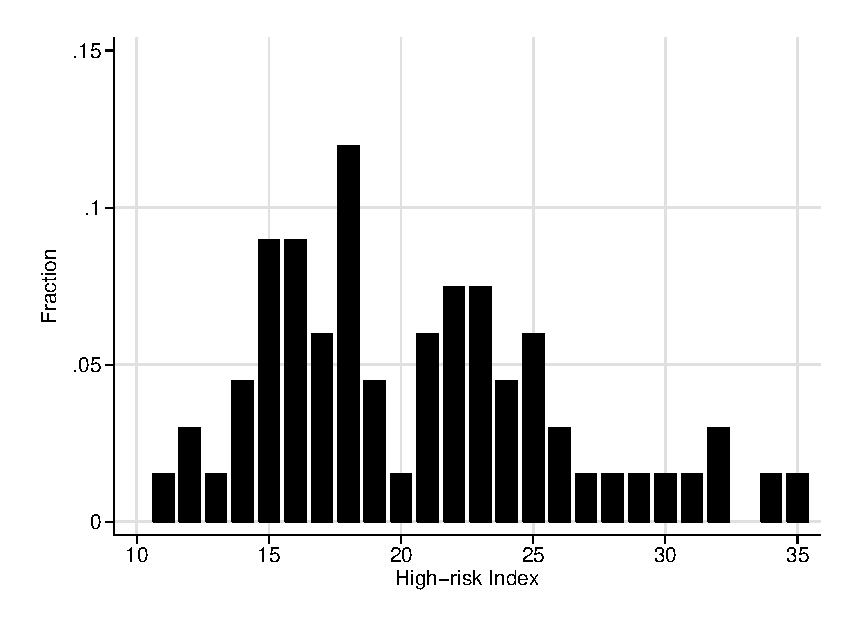
\includegraphics[width=.95\columnwidth]{output/care_hri.eps}
\floatfoot{
\footnotesize
\noindent Note: This plot shows the distribution of the High-risk Index (HRI) for CARE, which determined eligibility. Subjects were eligible if they had a score of 11 or more.}
	\end{figure}
\end{center}

\subsection{Randomization Protocol and Compromises} \label{appendix:randomization}

\noindent Randomization compromises throughout ABC's and CARE's implementations pose a challenge when evaluating the programs' effects. We discuss each case of compromise in detail. Figure~\ref{fig:abc-flow} and Figure~\ref{fig:care-flow} are flow charts that depict the sample from the first-phase randomization through the last data follow-up accounting for all cases of attrition and non-compliance. In Section~\ref{section:methodology},  we propose a methodology for adequately evaluating the programs while accounting for these compromises.\\

\noindent Although most randomization compromises occurred at early stages, this methodology also accounts for the fact that a few subjects were not in the sample either for the second-phase randomization or for the adult follow-ups. In Appendix~\ref{appendix:data}, we describe the sample reductions that attrition at different stages of the study generates and test potential differences between the subjects who completed data follow-ups and the subjects who did not.\\

\newgeometry{top=.1in, bottom=.1in, left=.1in, right=.1in}
	\begin{figure}[H]
		\caption{Randomization Protocol and Treatment Compliance, ABC} \label{fig:abc-flow}
		\centering
		\includegraphics[width=.92\columnwidth]{output/abc_Diagram.pdf}
	\end{figure}
	
	\begin{figure}[H]
		\caption{Randomization Protocol and Treatment Compliance, CARE} \label{fig:care-flow}
		\centering
		\includegraphics[width=.92\columnwidth]{output/care_Diagram.pdf}
	\end{figure}
\restoregeometry

\doublespacing

\noindent \textbf{Details on Figure~\ref{fig:abc-flow}:} Sources: \cite{Ramey_Collier_etal_1976_CarolinaAbecedarianProject, Ramey_Smith_1977_AJMD,Ramey_Campbell_1979_SR,Ramey_Campbell_1984_AJMD}, internal documentation of the program, and own calculations. Note: The variable $R$ represents randomization into treatment, $[R=1]$, or control, $[R=0]$, groups. After the original randomization, some subjects died or withdrew from the program early in life and were replaced. $R$ also includes those replacements. Arrows pointing outside of the diagram indicate subjects who left the study permanently. The variable $D$ represents participation in the preschool-age program. The variable $SR$ represents randomization into the school-age program, $[SR=1]$, or out of it, $[SR=0]$. Some subjects were not randomized at school age, $[SR=No]$. We use the term ``temporarily attrited" for subjects who did not participate in the study at school age, but were later interviewed in the age-21 followup. \\

\noindent \textbf{Details on Figure~\ref{fig:care-flow}:} Sources: \cite{Wasik_Ramey_etal_1990_CD}, internal documentation of the program, and own calculations. Note: The variable $R$ represents randomization into center-based childcare and family education, $[R=2]$, family education, $[R=1]$, or control, $[R=0]$. Arrows pointing outside of the diagram indicate subjects who left the study permanently. The variable $D$ represents participation in the corresponding group of the preschool-age program. The variable $SR$ represents those who participated in the school-age program, $[SR=1]$, or did not, $[SR=0]$. Unlike in ABC, there was no second-phase randomization in CARE. Rather, those in the center-based childcare and family education group and those in the family education group were automatically assigned to receive the school-age treatment. We use the term ``temporarily attrited" for subjects who did not participate in the study at school age, but were later interviewed in the age-21 followup.

\subsubsection{ABC}

\noindent Both the first and second phases of randomization were conducted at the family level, so pairs of siblings and twins were jointly randomized into either treatment or control groups.\footnote{Sibling pairs occurred when the two siblings were close enough in age such that both of them were eligible for the program.} Although we know that pairing was based on HRI, maternal IQ, maternal education, maternal age, and gender of the subject, we do not know the original pairs. The study collected an initial sample of 120 families. Twenty-two subjects did not complete the first-phase of treatment as initially assigned by the randomization (see Table~\ref{table:abccompromises}).\footnote{In Appendix~\ref{appendix:methodology}, we compare the observed baseline characteristics of the subjects in Table~\ref{table:abccompromises} to the observed baseline characteristics of the subjects who complied to the initial treatment assignment. We find little evidence of differences.}\\


\noindent Of these cases, there were four subjects assigned to treatment who left the study before any data on them was collected. In our main methodology, we assume that they are missing at random. Exercises assuming that these subjects had outcomes identical to the subject with the lowest outcome in the treatment group suggest that, even in this extreme scenario, there is little sensitivity of the estimates to including or deleting them (see Appendix~\ref{appendix:assessingcc}).\\

\noindent Second, four subjects died before age 5---two of them initially assigned to treatment and two of them initially assigned to control. For all of them, we observe baseline characteristics and any other data collected before their death. For methodological purposes, they represent cases of program attrition when we do not observe their outcomes.\\

\noindent Third, three subjects in the treatment group did not comply to treatment status. They are different from the four subjects who left the study before any data collection because we observe data collected for them from birth to age 8. Afterward, the program staff chose not to follow them anymore.\footnote{Informal conversations with the program's staff do not indicate a clear reason for this.} Therefore, these subjects remain in treatment sample until age 8 or before. After, they represent cases of program attrition, given that we do not observe them anymore. In Appendix~\ref{appendix:assessingcc} we find little sensitivity to adjusting for non-compliance of these children in the results we show for age 8 or before.\\

\begin{sidewaystable}[H] 
\begin{threeparttable}
\caption{Randomization Compromises, ABC}
\label{table:abccompromises}
\centering
\footnotesize
\begin{tabular}{lccccc} \toprule
Case & Initial Assignment & Compromise Description & Age at Departure & Data Availability & Methodology Assumption \\ \\ \midrule
1& Treatment & Left the study & 0 & None & Missing at random \\
2& Treatment & Left the study & 0 &  None & Missing at random \\
3& Treatment & Left the study & 0 &  None & Missing at random \\
4& Treatment & Left the study & 0 &  None & Missing at random \\ \midrule
5& Control  & Death (age 0), heart disease & 0 &  Baseline; before dead & Attrition after death \\
6&Control  & Death (age 0), heart disease & 0 &  Baseline; before dead & Attrition after death \\
7&Treatment & Death (age 0), SIDS & 0 &  Baseline; before dead & Attrition after death \\
8&Treatment  & Death (age 4), pedestrian accident & 4 &  Baseline; before dead & Attrition after death \\ \midrule
9&Treatment  & Non-compliance  & Do not depart &  Baseline; before age 8 & Attrition after age 8  \\
10&Treatment  & Non-compliance  & Do not depart&  Baseline; before age 8 & Attrition after age 8  \\
11&Treatment  & Non-compliance  & Do not depart &  Baseline; before age 8 & Attrition after age 8  \\ \midrule
12&Control        & Crossover from control to treatment & Do not depart &  Baseline; before age 8 & Attrition after age 8  \\ \midrule
13&Treatment   & 3 months of treatment & 3 months &   Baseline; after age 2 & Same as treatment group  \\  
14&Treatment &10 months of treatment & 10 months &   Baseline; after age 2 & Same as treatment group  \\
15&Treatment & 6 months of treatment &  6 months &   Baseline; after age 2 & Same as treatment group  \\ 
16&Treatment & 9 months of treatment & 9 months  &   Baseline; after age 2 & Same as treatment group  \\  \midrule
17&Control  & Left study at 54 months & 54 months &  Baseline; before 54 months & Attrition after 54 months \\ \midrule
18& Treatment       & Developmentally delayed at 6 months & 6 months &  No data after diagnosis & Dropped (non-eligible) \\ 
19&Treatment       & Developmentally delayed at 3 years & 3 &  No data after diagnosis & Dropped (non-eligible) \\ \midrule
20&Control       & Crossover from control to treatment & Do not depart &  Baseline, before age 8 & Attrition after age 8 \\ 
21&Control       & Crossover from control to treatment & Do not depart &  Baseline, before age 8 & Attrition after age 8   \\ \bottomrule
\end{tabular}
\begin{tablenotes}
\item Note: This table describes the various randomization compromises in ABC. For each subject, we display: the nature of the compromise, the available data, and the methodological assumption when accounting for non-compliance and program attrition. The case numbers do not have anything to do with individual identifiers of program participants. 
\end{tablenotes}
\end{threeparttable}
\end{sidewaystable}

\noindent Fourth, one subject initially assigned to control was enrolled into treatment. The mother wanted to work and the program staff decided to admit her child into center-based care.\footnote{Correspondence with the program officers stating this permission is available under request from the authors.} Both in terms of data collection and in terms of methodological purposes, this subject is analogous to the subjects in the third case.\footnote{The sensitivity analysis finding little evidence when adjusting for non-compliance includes this case.}\\

\noindent Fifth, four subjects in the treatment group did not complete treatment in its entirety. They were treated for at most 10 months. Except for follow-ups during childhood, which our main results do not use, we observe most of the data for these subjects. We avoid taking a stance on how beneficial the program was at each age, because we do not have a way to document this. Therefore, we assume that they were treated as other subjects in the treatment group.\footnote{If anything, this downward biases the effects of the program we estimate.} \\

\noindent Sixth, the family of one subject in the control group moved at age 54 months. We observe data before the family moved, so we consider the subject as part of the control group in any estimation before this event. Afterwards, we do not observe any data on the subject, so we consider her a case of program attrition.\\

\noindent Seventh, two subjects initially assigned to treatment status were diagnosed as developmentally delayed after 6 and 36 months of treatment. No data for them are available after the diagnosis. We drop them from the sample because they were not eligible to be part of the program.\\

\noindent Finally, two subjects initially assigned to the control group were admitted into treatment. Local authorities requested this because the children were considered highly at risk. Data on them are available from birth to age 8. Although they crossed over from the control group to the treatment group, we consider them to be members of the control group who attrited after age 8.\\

\noindent Analysis of each of these cases leads to the following conclusions. For four subjects, we do not have data to assess them as cases of program attrition, though sensitivity analyses suggest that the treatment effects of the program persist after assigning them the same outcome as the subjects who did the worst in the treatment group. For the subjects who did not comply to treatment, adjusting our estimates for non-compliance when data are available makes little difference. The remaining 14 subjects who did not complete treatment as initially assigned represent various cases of program attrition, for which we propose a correction methodology in Section~\ref{section:methodology}.\\

\noindent To increase the number of subjects in the sample, the program officers recruited additional subjects who were added to the program before the subjects were 6 months old. Our calculations indicate that there were eight replacements. We cannot distinguish in the data the subjects who were initially randomized from the replacement children and there is no documentation on how these subjects were recruited.\footnote{Three replacements are reported in \citet{Ramey_Campbell_1979_SR}. Three are documented in correspondence with the program officers, which is available from the authors upon request. The other two replacements are implied by the number of subjects who participated in the randomization protocol in each cohort.} After the various compromises, the sample consisted of 111 subjects: 53 in the treatment group and 58 in the control group. The observed characteristics for each subjects indicate that they were eligible for the program; all subjects in the sample have an HRI of 11 or above. \\

\noindent Prior to the second phase of randomization, 3 subjects in the first-phase control group and 3 subjects in the first-phase treatment group could not be located for follow-up. One subject in the control group and eight subjects in the treatment group of the first phase did not participate in the second phase but later agreed to participate in the data collections during adulthood. This yielded a sample of 96 subjects in the second phase: 49 in treatment and 47 in control. After the second-phase randomization, three subjects in the treatment group chose not to participate in the program, while all subjects in the control group adhered to their randomization status. \\

\subsubsection{CARE}

\noindent The randomization protocol in CARE had no major compromises.\footnote{\citet{Wasik_Ramey_etal_1990_CD,Burchinal_Campbell_etal_1997_CD}.} Of the 65 initial families, 23 were randomized to a control group, 25 to the family education treatment group (we do not consider this group in our combined ABC/CARE sample), and 17 to the family education and center-based childcare treatment group. Two families in the family education treatment group had twins who were jointly randomized, as in ABC. We document four cases of program attrition (see Table~\ref{table:care_compromises}).\footnote{In Appendix~\ref{appendix:methodology}, we compare the observed baseline characteristics of the subjects in Table~\ref{table:care_compromises} to the observed baseline characteristics of the subjects who complied to the initial treatment assignment. We find little evidence of differences.} For methodological purposes, we consider these subjects analogous to their corresponding cases in ABC. We do not present exercises to evaluate the sensitivity to non-compliance because there was none in CARE. Figure~\ref{fig:care-flow} illustrates CARE's randomization protocol and the presence of subjects throughout the data follow-ups.\\

\begin{sidewaystable}[H] 
\begin{threeparttable}
\caption{Randomization Compromises, CARE}
\label{table:care_compromises}
\centering
\footnotesize
\begin{tabular}{lcccc} \toprule
 Case & Initial Assignment & Compromise Description & Data Availability & Methodology Assumption \\ \\ \midrule
1&Family education & Death (age 0), unknown causes & Baseline & Attrition after dead \\
2&Center-based Childcare and Family Education  & Left study at age 5  & Baseline; before age 5 & Attrition after age 5 \\
3&Control & Move at 11 months old & Baseline; before 11 months & Attrition after 11 months \\
4&Center-based Childcare and Family Education & Move at 5 months old & Baseline; before 5 months & Attrition after 5 months \\
5&Center-based Childcare and Family Education & Move at age 5 & Baseline; before age 5 & Attrition after 5 \\ \bottomrule
\end{tabular}
\begin{tablenotes}
\item Note: This table describes the various randomization compromises in CARE. For each subjects, we display: the nature of the compromise, the available data, and the methodological assumption when accounting for non-compliance and program attrition. The case numbers do not have anything to do with individual identifiers of program participants. 
\end{tablenotes}
\end{threeparttable}
\end{sidewaystable}


\subsection{Program Description and Content}

\subsubsection{Goals}
\noindent The original goals of treatment were to prevent mental retardation by enhancing overall development from birth, in turn fostering school-readiness for an at-risk population.\footnote{Note that the clinical understanding of mental retardation was once associated with disadvantages that hindered early-life development \citep{Mental-Retardation_America_2004_BOOK_NYU}.} Additional curriculum goals were to (i) support language, motor, and cognitive development; (ii) minimize high-risk behaviors; and (iii) develop socio-emotional competencies considered crucial for school success including task-orientation, communicative competence, independence, and prosocial behavior.\footnote{\citet{Ramey_Collier_etal_1976_CarolinaAbecedarianProject, Ramey_etal_1985_Project-CARE_TiECSE, Sparling_1974_Synth_Edu_Infant_SPEECH, Wasik_Ramey_etal_1990_CD, Ramey-etal_2012-ABC}.} Implementation of ABC's and CARE's educational treatments evolved each successive year as program staff evaluated ongoing outcome data.\footnote{ \citet{Ramey-etal_1975_AJoMD, Finkelstein_1982_Day_Care_YC, McGinness_1982_Language-Poverty-Child,Haskins_1985_CD}.}\\


\subsubsection{Daily Schedule}
\noindent For both ABC and CARE, FPGC was open to families from 7:45 a.m. to 5:30 p.m., 5 days per week and 50 weeks per year.\footnote{\citet{Ramey_Collier_etal_1976_CarolinaAbecedarianProject, Ramey_etal_1985_Project-CARE_TiECSE}.} Subjects were offered free transportation to and from the center. A driver and second adult staffed each vehicle (one van and two station wagons) equipped with child safety seats.\footnote{\citet{Ramey_Campbell_1979_SR,abc2014-2015interviews}.} Approximately 65\% of treated ABC families utilized the free transportation.\footnote{\citet{Barnett_Masse_2002_benefitcost}.} Vehicles typically arrived by 9:00 a.m. to the center and departed around 3:45 p.m.\footnote{\citet{Ramey-et-al_1977_Intro-to-ABC}.} At FPGC, ABC and CARE treatment-group subjects received breakfast, lunch, and a snack planned by a nutritionist.\footnote{ \citet{Haskins_1985_CD, Bryant_et_al_1987_Carolina_Approach_TIECSE, Ramey-et-al_1977_Intro-to-ABC}.} Meals were catered by off-site kitchens. Infants received iron-fortified formula  until doctors advised adding solid food. The control-group subjects also received an unlimited amount of iron-fortified formula until approximately 15 months of age.\footnote{\citet{Campbell_Conti_etal_2014_EarlyChildhoodInvestments,abc2014-2015interviews}.}\\

\subsubsection{Program Staff and Physical Space}
\noindent To promote trust in FPGC within the subjects' families, staff were recruited from the local community.\footnote{\citet{Ramey-et-al_1977_Intro-to-ABC, Bryant_et_al_1987_Carolina_Approach_TIECSE, Feagans_1996_Childrens-Talk,abc2014-2015interviews}.} Infant and toddler caregivers and preschool teachers demonstrated varied educational backgrounds ranging from high school graduation to master's degrees. Their average professional working experience with young children was 7 years.\footnote{\citet{Ramey_McGinness_etal_1982_Abecedarianapproach, Ramey_etal_1985_Project-CARE_TiECSE, Wasik_Ramey_etal_1990_CD}.} All classroom staff participated in extensive training and were closely observed by FPGC's academic staff, as part of a broad variety of ongoing clinical and social research related to early childhood education, psychology, and health. In ABC, child-caregiver ratios varied by age: 3:1 for infants up to 13 to 15 months of age; 4:1 for toddlers up to 36 months; and 5:1 or 6:1 for children aged 3 to 5 years, depending on cohort size.\footnote{\citet{Ramey-et-al_1977_Intro-to-ABC,Ramey_Campbell_1979_SR,Ramey_McGinness_etal_1982_Abecedarianapproach}.} Child-caregiver ratios were similar in CARE.\footnote{\citet{Burchinal_Campbell_etal_1997_CD, Ramey_etal_1985_Project-CARE_TiECSE}.}\\

\noindent The ABC and CARE staff included a program director, a secretary, 12 to 14 teachers and assistant teachers, 3 administrative staff members, and a transportation supervisor.\footnote{\citet{Ramey-et-al_1977_Intro-to-ABC,Ramey_McGinness_etal_1982_Abecedarianapproach, Bryant_et_al_1987_Carolina_Approach_TIECSE}.} Lead caregivers and teachers had bachelor's or master's degrees. Teacher aides, recruited from the local community, held high school diplomas (at minimum) and were comparatively well-compensated in the childcare field. They remained a stable treatment component throughout the study. After 1980, following revisions to FIDCR regarding minimum requirements for early childhood education staff, several teacher aides pursued and received undergraduate degrees and became lead teachers. All classroom staff were supervised daily, received weekly mentoring, and professional development from outside consultants..\footnote{\citet{Obrien-Sanders_1974_ABC-brochure, Ramey_etal_1985_Project-CARE_TiECSE, Sanders-Stokes_1979_Status-Report,Klein-Sanders_1982_Status-Report,abc2014-2015interviews}.}\\

\noindent Infant nurseries, toddler rooms, and preschool classrooms were housed on different floors of FPGC. Early reports indicate that FPGC allocated two floors to ABC, but later reports indicate the use of three floors.\footnote{\citet{Ramey_Smith_1977_AJMD,Ramey_Campbell_1979_SR,Ramey_1981_Modification}.} Two infant nurseries were staffed by five adults in a suite of four adjoining rooms: two sleeping rooms contained seven cribs each, while the other two rooms were designated for activities.\footnote{ \citet{Ramey-et-al_1977_Intro-to-ABC}.} The four rooms opened into a large, shared space with feeding tables, an area for food preparation, and a couch.\footnote{\citet{Ramey_Campbell_1979_SR}.} Offices for the medical staff, along with two examining rooms and facilities for laboratory tests were located around the corner from the infant nurseries.\footnote{\citet{abc2014-2015interviews}.} Two multi-age toddler rooms were located one floor below the infant nurseries. One room served children who were 1 to 2 years old and the other served children 2 to 3 years old.\footnote{\citet{Ramey_Smith_1977_AJMD,Ramey_Campbell_1979_SR}.} 3-year-olds were housed in a closed classroom near the toddler rooms. On the lowest floor, 4-year-olds shared an open classroom with a public kindergarten program; the two classes were separated by a long, low bookcase. In CARE, two floors of FPGC were allocated to nurseries and classrooms. A mixed-age classroom design was implemented combining children ages 1 and 3, and children ages 2 and 4. Teacher-child ratios for these ages remained 1:5. FPGC offered two outdoor play areas for both ABC and CARE: one for children up to age 3, and the other for older children.\footnote{\citet{Ramey_Campbell_1979_SR,Ramey_McGinness_etal_1982_Abecedarianapproach}.}\\

\subsubsection{Approach to Child Development}
%Direct from the paper
\noindent Curriculum delivery enabled a highly customized learning experience for treated subjects in both ABC and CARE. Infant caregivers recorded child observations on progress charts and collaborated with FPGC's curriculum developers and academic researchers to rotate learning activities every 2 to 3 weeks for each treated subject.\footnote{\citet{Ramey_Collier_etal_1976_CarolinaAbecedarianProject,Campbell_Ramey_1994_CD}.} Preschool rooms featured intentionally organized environments to promote pre-literacy and access to a rich set of learning tools. The full-day curriculum emphasized active learning experiences, dramatic play, and pre-academics. Frequent 1:1 or 2:1 child-adult interactions prioritized language development for social competence. For ages 3 through 5, as the cohorts approached public school entry, classroom experiences were increasingly structured  towards the development of pre-academic skills and ``socio-linguistic and communicative competence.''\footnote{\citet{Ramey-et-al_1977_Intro-to-ABC, Haskins_1985_CD, Ramey_1981_Modification, Ramey_Campbell_1979_SR, Ramey_Smith_1977_AJMD, Ramey_McGinness_etal_1982_Abecedarianapproach, Sparling_Lewis_1979_BOOKLearninggamesFirstThree,Sparling_Lewis_1984_BOOKLearningGamesThreesFours}.} FPGC offered a summer program before the start of kindergarten designed to target specific skills to ensure success in a kindergarten classroom (e.g., lining up when exiting the classroom). This program was available to subjects in both the center-based childcare and family education group and the family education group.\footnote{\citet{Ramey_etal_1985_Project-CARE_TiECSE}.} \\

\noindent ABC's and CARE's learning programs were influenced by key developmental theorists.\footnote{These include including Bowlby, Piaget, and Vygotsky. \citep{Sparling_1974_Synth_Edu_Infant_SPEECH,Mcginness_1981_Developing,abc2014-2015interviews}.} All four ABC cohorts and two CARE cohorts participated in curriculum developers Sparling and Lewis' ``LearningGames for the First Three Years.''\footnote{ \citet{Sparling_Lewis_1979_BOOKLearninggamesFirstThree}.} The ``LearningGames'' were implemented daily by infant and toddler caregivers in 1:1 child-adult interactions. Each ``LearningGames'' activity stated a developmentally-appropriate objective, the necessary materials, directions for teacher behavior, and expected child outcome. The activities were designed for use both indoors and outdoors, while dressing, eating, bathing, or during play.\footnote{\citet{Ramey_Campbell_1979_SR, Ramey_1981_Modification,Sparling_Lewis_1979_BOOKLearninggamesFirstThree}.}\\

\noindent Supplemental curricula for preschool rooms varied throughout the study, and included ``Cook and Learn,'' ``Peabody Early Experiences Kit,'' ``GOAL Math Program,'' and ``My Friends and Me.''\footnote{ \citet{Greenberg_Epstein_1973_BOOKBridgestoreading,Karnes1973,Dunn_Chun_etal_1976_BOOKPeabodyearlyeducation,Davis_1977_BOOKMyfriends,Wallach_1976_Teaching-All-Children}.}
%SK notes to co-authors: I'm currently waiting for info from Lynne Vernon-Feagans to potentially include a social worker to the list of staff!

\noindent CARE subjects randomized into the center-based childcare and family education group or the family education group also received home visits designed to transmit information on child development and skills involved with parenting including strategies for parent-child interactions based on ``LearningGames" activities and problem-solving techniques.\footnote{\citet{Bryant_et_al_1987_Carolina_Approach_TIECSE, Wasik_Ramey_etal_1990_CD, Burchinal_Campbell_etal_1997_CD}.} Home visitors were trained to ensure they were able to form a strong relationship with the parent and successfully implement the curriculum.\footnote{\citet{Bryant_et_al_1987_Carolina_Approach_TIECSE}.} The visits lasted about an hour, and occurred weekly until the child was 3 years old. After age 3, the home visits were less frequent and depended on the preferences of the parents. They were usually about once a month after age 3.\footnote{\citet{Bryant_et_al_1987_Carolina_Approach_TIECSE, Wasik_Ramey_etal_1990_CD, Burchinal_Campbell_etal_1997_CD}.} \\

\subsubsection{Medical Care and Nutrition}
%Direct from the paper
ABC and CARE provided comprehensive on-site medical care because it was conducted in conjunction with a longitudinal medical research study on infectious respiratory diseases in group environments.\footnote{\citet{Henderson-et-al_1982_NEJoM}.} Treatment group children were monitored daily for signs of illness. All treated children received medical care while attending center-based childcare; the first ABC cohort of control-group children also received medical care during the program's first year of implementation.\footnote{\citet{Ramey_Collier_etal_1976_CarolinaAbecedarianProject, Bryant_et_al_1987_Carolina_Approach_TIECSE, Ramey_Campbell_1991_childreninpoverty,Campbell_Ramey_1994_CD}.}$^{,}$\footnote{Subjects in both the treatment and control groups of the first cohort received free medical care provided by ABC. The control group of the first cohort only received medical care in the first year of the program; the treatment group of the first cohort received medical care for all years of the program. In the subsequent cohorts, only subjects in the treatment group received free medical care provided by ABC. Both CARE cohorts of treated subjects received medical care.}\\
%Direct from the paper

\noindent In ABC, primary pediatric care was provided by a family nurse practitioner and a licensed practical nurse, both under the supervision of one pediatrician who was on continuous duty at the center.\footnote{\citet{Haskins-et-al_1978_JoPP}.} In CARE, the medical staff included two pediatricians, a family nurse practitioner, and a licensed practical nurse.\footnote{\citet{Bryant_et_al_1987_Carolina_Approach_TIECSE}.} The medical staff provided regularly scheduled check-ups, immunizations, parental counseling, and initial assessment of illnesses.\footnote{\citet{Ramey-et-al_1977_Intro-to-ABC, Bryant_et_al_1987_Carolina_Approach_TIECSE}.} The treatment group received standard check-ups when they were 2, 4, 6, 9, 12, 18, and 24 months old and annually thereafter. While in treatment, they also received the standard immunizations.\footnote{\citet{Bryant_et_al_1987_Carolina_Approach_TIECSE, Campbell_Conti_etal_2014_EarlyChildhoodInvestments}.} In ABC, a licensed practical nurse visited classrooms for up to two hours on a daily basis to monitor the subjects' health status.\footnote{\citet{Sanyal_Henderson_etal_1980_JoPediatrics}.} Although this medical care was offered to the treatment-group families free of charge, it was the policy of the medical staff to refer families to a community hospital for serious treatment. While ABC and CARE provided aspirin, immunizations, and basic medicines, families were responsible for purchasing any prescription medication subjects required. There are no data currently available on treatment received for serious conditions or use of prescription medication.  \\

\noindent Infants were supplied with iron-fortified formula. Children older than 15 months of age were provided breakfast, lunch, and an
afternoon snack all planned by a nutritionist.\footnote{\citet{Bryant_et_al_1987_Carolina_Approach_TIECSE, Campbell_Conti_etal_2014_EarlyChildhoodInvestments,abc2014-2015interviews}.} Control families received diapers for up to three years and unlimited iron-fortified bottled formula through 15 months.\footnote{\citet{Ramey_Collier_etal_1976_CarolinaAbecedarianProject,Ramey_Campbell_1979_SR, Ramey_etal_1985_Project-CARE_TiECSE}.}

\subsubsection{School-age Treatment}

\noindent The ABC subjects were randomization into a second-phase, school-age treatment (95 subjects continued to this stage of treatment). The CARE subjects in the center-based childcare and family education group and the family education group received the school-age treatment without randomization. The school-age treatment lasted for the first three years of elementary school and consisted of home visits conducted by a Home/School Resource Teacher.\footnote{\cite{Burchinal_Campbell_etal_1997_CD}.} These visits were structured to increase exposure to reading and mathematics and promote parental involvement in the academic process.\\

\noindent The curriculum was delivered through sets of activities that developed skills such as handwriting, phonics, and math facts.\footnote{There were about 60 activities per year. See \cite{Campbell-Ramey_1989_Preschool-vs-School-age} for details.} Teachers worked to encourage parental involvement in the subjects' academics and provided incentives to families to comply with the treatment, such as giving gift certificates to restaurants and books for the subjects upon the completion of activity packets. \\

\noindent Teachers had graduate-level education, training in special education, \textit{or} were qualified to act as consultants for in-school teachers to address any problems that arose.\footnote{\cite{Ramey_Campbell_1991_childreninpoverty}.} They met with parents at home and with teachers in the schools to deliver new activities for the parents to complete with their children and discuss the child's level of success with the previous set of activities. In addition, they helped parents with issues such as adult literacy, housing, and medical care. Thus, the teacher had a dual role as a parent educator and an advocate for the subject in their educational institution.

\subsection{Control Substitution}

\noindent In ABC, the families of almost $70\%$ of the control-group subjects enrolled their children in alternative center-based childcare. In CARE, $74\%$ of families in the control group and $62\%$ of families in the family education group enrolled their children in alternative center-based childcare. We refer to this phenomenon as control substitution; accounting for it is fundamental when evaluating the program, as we argue in Section~\ref{section:methodology}. In this Appendix, we thoroughly describe the characteristics and costs of the childcare centers providing alternative treatment, in order to create a comparison with the treatments offered by ABC and CARE.\\

\noindent Most of the families in the ABC and CARE control groups enrolled their children in alternative preschool that received federal subsidies and, therefore, were regulated. Figure~\ref{fig:ccabc} and Figure~\ref{fig:cccare} show the amount of enrollment into subsidized and non-subsidized care for ABC and CARE, respectively. Subsidized centers were required to have trained staff who were able to implement curricula designed to enhance cognitive, social, and linguistic competence in disadvantaged children.\footnote{\citet{Burchinal_etal_1989_CD_Daycare-Pre-K-Dev}.} Thus, we consider these centers to offer high-quality center-based childcare.

	\begin{figure}[H]
		\caption{Average Number of Months in Alternative Preschool, ABC Control Group} \label{fig:ccabc}
		\centering
		\includegraphics[width=.8\columnwidth]{output/blackwhite_CCnumber.eps}
\floatfoot{
\footnotesize
\noindent Note: This figure describes the take-up of alternative preschool by families in the ABC control group. The vertical axis represents the average number of months per year the subjects of the control group spent in alternative preschool. Subsidized centers were highly regulated and, therefore, relatively high-quality. Non-subsidized childcare services were center-based but not regulated. Other sources of childcare could have included care by parents, relatives, or non-relatives.}
	\end{figure}

	\begin{figure}[H]
		\caption{Average Number of Months in Alternative Preschool, CARE Control and Family Education Groups} \label{fig:cccare}
		\centering
		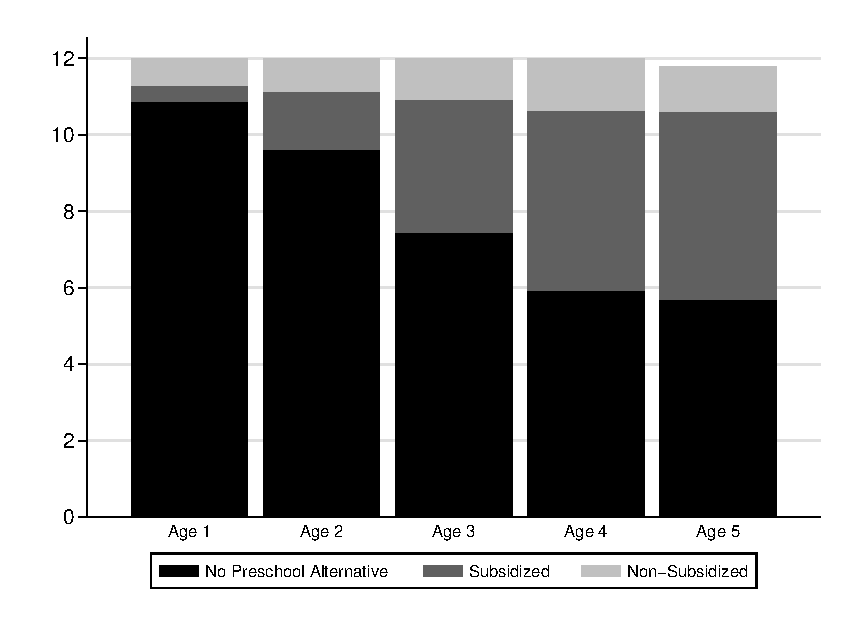
\includegraphics[width=.8\columnwidth]{output/blackwhite_CCnumber_care.eps}
\floatfoot{
\footnotesize
\noindent Note: This figure describes the take-up of alternative preschool by families in the CARE family education and control groups. The vertical axis represents the average number of months per year the subjects of the control group spent in alternative preschool. Subsidized centers were highly regulated and, therefore, relatively high-quality. Non-subsidized childcare services were center-based but not regulated. Other sources of childcare could have included care by parents, relatives, or non-relatives.}
	\end{figure}
	
Table~\ref{table:controlsubscharacteristics} shows baseline characteristics between the control-group subjects who were enrolled in alternative preschool and those who stayed at home. The control-group children who attended alternative preschool were marginally more advantaged, with the most stark difference being maternal employment. This is seen across genders, but is only significant for the female and pooled samples. The males who are enrolled in alternative preschool have mothers with higher IQ scores, but lower parental income indicating lack of spousal support, which is evident by the fewer number of fathers present in that same group. Those who were enrolled in alternative preschools also had more siblings.

\begin{sidewaystable}[H]
\centering
\begin{threeparttable}
\caption{Baseline Characteristics and Control Substitution}\label{table:controlsubscharacteristics}
\begin{tabular}{l c c}
\toprule
Characteristic & \mc{2}{c}{Control Substitution} \\
& No & Yes \\
& $ N=19 $ & $ N=55 $ \\
\midrule
Mother's Yrs. of Edu. &      9.74 &     10.35 \\
                     & (     0.43) & (     0.26)  \\
Mother's Age &     21.42 &     20.27 \\
                     & (     1.79) & (     0.63)  \\
Mother's IQ &     82.00 &     85.60 \\
                     & (     2.32) & (     1.33)  \\
HRI Score &     20.95 &     21.60 \\
                     & (     1.46) & (     0.81)  \\
Number of Siblings &      1.00 &      0.62 \\
                     & (     0.38) & (     0.13)  \\
Male &      0.47 &      0.51 \\
                     & (     0.12) & (     0.07)  \\
Birth Year &   1975.58 &   1975.73 \\
                     & (     0.68) & (     0.32)  \\
Apgar Score, 1 min. &      7.47 &      7.62 \\
                     & (     0.43) & (     0.21)  \\
Apgar Score, 5 min. &      8.63 &      8.98 \\
                     & (     0.26) & (     0.14)  \\
\bottomrule
\end{tabular}
\begin{tablenotes}
\item Note: This table describes baseline characteristics for the children in the control group, by gender and by their alternative preschool enrollment status. The number of subjects in these groups are listed at the top of the table. Asymptotic standard errors are in parentheses. The reported $p$-values are from two-sided tests of difference of means. The means are bolded if the difference is significant at the 10\% level.
\end{tablenotes}
\end{threeparttable}
\end{sidewaystable}

\subsubsection{Regulation}  \label{appendix:tetanus}

\noindent During the period when both ABC and CARE were active, North Carolina had an active, high-quality system of public childcare for vulnerable families funded by several public programs. Examples include Title IV-A of the Social Service Administration (SSA), Aid to Families with Dependent Children (AFDC), and Title IV-B of Child Welfare Services. These funding efforts were amplified in 1975 by Title XX of the SSA, Social Services Block Grant, which was the main federal source of childcare financing in the U.S. when ABC and CARE were active.\footnote{\citet{Robins_1988_Federal-Child-Care}.}\\

\noindent Federally funded childcare services were regulated according to FIDCR standards, which defined stringent regulation for center-based programs for children between the ages of 3 and 6.\footnote{\citet{Department-of-Health_1968_DayCareRequirements}.} These requirements were enforced.\footnote{\citet{Kuperman_2015_Clifford-Russell-Interview}.} Additionally, North Carolina had a mandatory licensing law for childcare facilities. While FIDCR applied to centers for older children (between the ages of 3 and 6), the North Carolina regulation only applied to centers serving children below the age of 3. The relative weakness of this regulation is not very relevant for our study because treatment substitution occurred mostly after age 3 (see Figure~\ref{fig:ccabc} and Figure~\ref{fig:cccare}).\footnote{\citet{NCGA_1971_House-Bill-100}.} Table~\ref{table:staff} compares a widely-used quality standard, the child-staff ratio, between the North Carolina and FIDCR standards and the actual ABC and CARE numbers. \\

%Not in main paper
\begin{table}[H]
\centering
\caption{Child-Staff Ratios for North Carolina, FIDCR, and Actual ABC and CARE Ratios}
\label{table:staff}
\begin{threeparttable}
\begin{tabular}{lccc}
\toprule
 &NC Standards & FIDCR &  ABC and   \\
Age	& Level I &  Standards  & CARE Ratios\\ \midrule
0--1	& 6:1*	&  				& 	3:1					\\
1--2	& 8:1* 	& 				&   4-5:1				\\
2--3	& 12:1* & 				& 	4-5:1				\\
3--4	& 15:1 	& 		5:1*	& 	4-5:1 				\\
4--5	& 20:1 	& 		7:1*	& 	5-6:1 				\\
5--6 & 25:1  &		7:1*	&	5-6:1				\\
\bottomrule
\end{tabular}
\begin{tablenotes}
\footnotesize
Sources: \cite{Department-of-Health_1968_DayCareRequirements,NCGA_1971_House-Bill-100,Ramey-et-al_1977_Intro-to-ABC,Ramey_Campbell_1979_SR,Ramey_McGinness_etal_1982_Abecedarianapproach, Burchinal_Campbell_etal_1997_CD}.\\
Note: The starred ratios represent the ones we believe were the most relevant for the ABC control-group subjects and the CARE control-group and family-education-group subjects.
\end{tablenotes}
\end{threeparttable}
\end{table}

\subsubsection{Costs}
% Need citations
\noindent Previous papers have used childcare cost rates that are not specific to North Carolina and do not account for the contemporaneous structure of the subsidies. We use the local subsidy rates that were in place when the ABC subjects were in preschool to impute different costs of the alternative preschools. These costs depend on the specific preschool attended and the eligibility of the families to receive the subsidies. \\

\noindent When ABC and CARE were in operation, center-based childcare was subsidized by several federal programs (the Department of Social Services categorized these programs as Child Welfare, AFDC, and Work Incentive Programs).\footnote{\citet{NC-State-Dept_1972_Licensed-Day-Care}.} However, our calculations of the cost of alternative preschool are simplified by the fact that the subsidies were centralized and regulated by the County Department of Social Services. Those departments used a uniform subsidy rate, regardless of the origin of the funds.\footnote{\citet{Ad-Hoc-NC_1974_Letter}.} We collected information about the subsidy rate at the time, which approximates the price of the centers, as centers pegged their fees and services to the maximum subsidy rate. Moreover, we know which centers each ABC control subject attended. We interviewed North Carolina childcare staff and academics that study childcare to document which of those centers were subsidized and regulated at the time.\footnote{\citet{Kuperman_2015_Clifford-Russell-Interview,Kuperman-Hojman_2015_Hodgers-Interview}.} For subsidized centers, we impute the maximum Department of Social Services fee established at the time: \$633/month in 2014 USD.\footnote{\citet{Ad-Hoc-NC_1974_Letter,Comm-Plan-Serv_1973_Durhams-Share}.} For non-subsidized centers, we impute the mean of costs for Level-1 centers (minimum accepted quality level) according to a 1982 North Carolina study of the cost of childcare: \$298/month in 2014 USD.\footnote{\citet{NC-Admin-Branch_1982_Day-Care-Cost-Study}.} Although the information in this survey is not ideal for assessing the cost of subsidized preschools for CARE, as the subsidies greatly changed after the end of FIDCR (1981), it provides an approximation for assessing the cost of the non-subsidized centers. \\

\noindent Finally, we determine if the families paid the costs themselves or if they were subsidized, in which case we also add deadweight costs. We consider if a subject was eligible for subsidies if the family lived in poverty according to the federal guidelines and all parents living at home worked. If a family is deemed eligible, then we assume the child's preschool was fully subsidized using the rates described above without additional subsidies.\\

\subsection{Data} \label{appendix:data}

In Table~\ref{tab:ecvars_1} through Table~\ref{tab:adultvars_2}, we summarize the data availability for both ABC and CARE. The data collection processes in both programs were analogous by design. For both programs, the treatment and control groups were followed into adulthood with relatively low attrition. For ABC, subjects were followed annually through elementary school and at ages 12, 15, 21, and 30. Health and administrative crime data were collected when the subjects reached their mid-30s. For CARE, the exact same follow-ups are available with the exception of the age 15 follow-up.\\

\begin{sidewaystable}[H]
\small
\caption{Early Childhood Data (Part I)}
\label{tab:ecvars_1}
\centering
\begin{adjustbox}{max width=\textwidth, max height=\textheight,keepaspectratio}
\begin{threeparttable}
\tiny
\begin{tabular}{L{3cm} C{3.5cm} C{4cm} C{1.5cm} C{1.5cm}  C{6cm}}
\toprule
\textbf{Category}	&	\textbf{Sub-Category}	&	\textbf{Description}	&	\textbf{ABC Age}  	&  \textbf{CARE Age}  & 	\textbf{Measure}	\\ \midrule
Demographics	&	Gender	&	Gender of subject	&	Birth, 18, 30, 42, 54	&	 Birth, 18, 30, 42, 54	&	Demographic Interview	\\
	&	\\
	&	Race	&	Race/Cultural identity of subject	&	Birth, 18, 30, 42, 54	&	 Birth, 18, 30, 42, 54	&	 Demographic Interview\\
	&	\\
	&	Birth Date	&	Date of birth of subject	&	Birth, 18, 30, 42, 54	& 	Birth, 18, 30, 42, 54	&	 Demographic Interview	\\ \midrule
Cognitive Assessments	&	Language Ability	&	Auditory association, Verbal expression, etc. 	&	36, 42, 48, 54	&	30, 42, 54	&	ITPA$^{ABC}$, GPB$^{ABC}$, PLP$^{ABC}$, MSCD \\
	&	\\
	&	Intelligence Levels	&	SBIS 	&	24, 36, 48, 60	&	24, 36, 48, 60	&	SBIS	\\
	&		&	WPPSI	&	60	&	60	&	WPPSI	\\
	&		&	BSID 	&	3, 6, 9, 12, 18, 24	&	6, 12, 18, 24		&	BSID	\\
	&		&	UOSPD	&	15	&	- 	&	UOSPD$^{ABC}$	\\
	&		&	RPM	&	60	&	-	&	RPM$^{ABC}$	\\
	&	\\
	&	Quantitative	 &	BSID 	&	3, 6, 9, 12, 18, 24	&	6, 12, 18, 24		&	BSID	\\
	&		&	MSCD 	&	30, 42, 54		&	30, 42, 54	&	MSCD	\\
	&	\\
	&	Memory	&	BSID 	&	3, 6, 9, 12, 18, 24	& 	6, 12, 18, 24		&	BSID	\\
	&		&	MSCD 	&	30, 42, 54	&	30, 42, 54	&	MSCD	\\
	&	\\
	&	Motor Development	&	BSID 	&	3, 6, 9, 12, 18, 24	&	6, 12, 18, 24		&	BSID\\
	&		&	MSCD 	&	30, 42, 54	&	30, 42, 54	&	MSCD	\\
	& 	\\
	&	Critical Thinking	&	Curiosity	&	30, 36, 42, 48, 54, 60, 66, 72	& - &	Infant Behavior Inventory$^{ABC}$	\\ \midrule
Non-Cognitive Assessments	&	Social Skills	&	Positive social response	&	30, 36, 42, 48, 54, 60, 66, 72	&	6, 12, 18, 24		&	Infant Behavior Inventory$^{ABC}$, Bayley Infant Inventory$^{CARE}$	\\
	&		&	Creativity	&	30, 36, 42, 48, 54, 60, 66, 72	&	- 	&	Infant Behavior Inventory$^{ABC}$	\\
	&	\\
	&	Self-Control	&	Locus of control	&	3, 18	&	6, 18	& 	RIES	\\
	&		&	Distractibility, Attentiveness	&	30, 36, 42, 48, 54, 60, 66, 72	&	6, 12, 18, 24		&	Infant Behavior Inventory$^{ABC}$, Bayley Infant Inventory$^{CARE}$	\\
	&	\\
	&	Emotional Health	&	KRT	&	24, 36, 48, 60	&	24, 30, 36, 42, 48, 60	&	KRT	\\
	&	\\
	&	Self-Consciousness	&	Self-consciousness	&	30, 36, 42, 48, 54, 60, 66, 72	&	-	&	Infant Behavior Inventory$^{ABC}$	\\
\bottomrule
\end{tabular}
\begin{tablenotes}
\scriptsize
\item Sources: Authors' description. \\	
\item Note: This table describes the main categories of variables that were measured for ABC and CARE subjects up to age 6. ABC and CARE ages are measured in months. This is not an exhaustive list of variables, nor does it include variables from auxiliary data. Instruments or questionnaires available for only one of the studies are indicated with the superscript $^{ABC}$ or $^{CARE}$.  \textbf{Abbreviations are as follows.} ITPA: Illinois Test of Psycholinguistic Ability. GPB: Gordon Psycholinguistic Battery. PLP: Preschool Language Performance. MSCD: McCarthy Scales of Children's Development. BSID: Bayley Scales of Infant Development and Infant Behavior. UOSPD: Uzgiris-Hunt Ordinal Scales of Psychological Development. RPM: Raven's Progressive Matrices. RIES: Rotter's Internality-Externality Scale. KRT: Kohn and Rosman Test Behavior Inventory.
\end{tablenotes}
\end{threeparttable}
\end{adjustbox}
\end{sidewaystable}




\begin{sidewaystable}[H]
\small
\caption{Early Childhood Data (Part II)}
\label{tab:ecvars_2}
\centering
\begin{adjustbox}{max width=\textwidth, max height=\textheight,keepaspectratio}
\begin{threeparttable}
\tiny
\begin{tabular}{L{3cm} C{3.5cm} C{4cm} C{1.5cm} C{1.5cm}  C{6cm}}
\toprule
\textbf{Category}	&	\textbf{Sub-Category}	&	\textbf{Description}	&	\textbf{ABC Age}  	&  \textbf{CARE Age}  & 	\textbf{Measure}	\\ \midrule
Family Environment	&	Family Members	&	Number of primary caretakers	&	Birth, 18, 30, 42, 54	&	18, 30, 42, 54, 60	&	Demographic Interview	\\
	&		&	Relationship with family members, including father, mother, siblings, etc.	&	Birth, 18, 30, 42, 54	&	18, 30, 42, 54, 60	&	Demographic Interview	\\
	&		&	Number of siblings	&	Birth, 18, 30, 42, 54	&	Birth, 18, 30, 42, 54, 60	&	Demographic Interview	\\
	&		&	Marital status of parents	&	Birth, 18, 30, 42, 54	&	Birth, 18, 30, 42, 54, 60	&	Demographic Interview	\\
	&		&	Marital conflicts between parents	&	6, 18	&	Birth, 6, 18, 36	&	Demographic Interview$^{CARE}$, Parental Attitudes Research Inventory	\\
	&		& Father at home & 18, 30, 42, 54  & 18, 30, 42, 54, 60 & Demographic Interview \\
	&	\\
	&	Family Economic Environment	&	Parents' occupation	&	Birth, 18, 30, 42, 54	& 	Birth, 18, 30, 42, 54, 60		&	Demographic Interview	\\
	&								& Mother works & 18, 30, 42, 54 & 18, 30, 42, 54, 60 & Demographic Interview \\
	&		&	Source of child support	&	Birth, 18, 30, 42, 54	&	18, 30, 42, 54, 60	&	Demographic Interview	\\
	&		&	Family income	&	Birth, 18, 30, 42, 54	&	Birth, 18, 30, 42, 54, 60	&	Demographic Interview	\\
	&	\\
	&	Parents and Home Environment & Parents' authority, warmth, family conflict, etc. & 6, 18, 30, 42, 54 & 6, 12, 18, 30, 42, 54 & Parent Interview \\
	&	\\
	&	Family Social Status	&	Parents' education background	&	Birth, 18, 30, 42, 54	&	Birth, 18, 30, 42, 54, 60		&	Demographic Interview	\\
	&		&	Risk taking of family members	&	Birth	&	- 	&	Parent Interview$^{ABC}$	\\
	&	\\
	&	Family Members' Physical Health	&	Health issues of parents	&	Birth	&	Birth	&	Parent Interview	\\
	&		&	Pregnancy history	&	Birth	&	Birth	&	Parent Interview	\\ \midrule
Childcare	&	Day-care Experience	&	Time and location of childcare, Age when begin	&	Birth, 18, 30, 42, 54	&	18, 30, 42, 54	&	Demographic Interview	\\
			&						& 	Home visits &	-	&	6, 18, 30, 42, 54, 60	& Home Visit Data$^{CARE}$ \\
	&	\\
	&	Parental Care	&	Maternal warmth, Maternal involvement with child	&	6, 18, 30, 42, 54	&	6, 12, 18, 30, 42, 54	&	Home Stimulation	\\
	&		&	Provision of appropriate play materials	&	6, 18, 30, 42, 54	&	 6, 12, 18, 30, 42, 54	&	Home Stimulation	\\
	&		&	Avoidance of restriction and punishment	&	6, 18, 30, 42, 54	&	6, 12, 18, 30		&	Home Stimulation	\\
	&		&	Authoritarian control	&	6, 18, 30, 42, 54	&	6, 12, 18, 30, 36, 42, 102		&	Home Stimulation, Parental Attitudes Research Inventory	\\
	&		&	Democratic attitudes	&	6, 18	&	6, 18, 36	&	Parental Attitudes Research Inventory	\\
	&		&	Hostility and rejection	&	6, 18	&	6, 18, 36	&	Parental Attitudes Research Inventory	\\
	&		&	Parents' knowledge of childcare	&	Birth	&	-	&	Parent Interview$^{ABC}$	\\ \midrule
Physical Health	&	Growth Data	&	Height, Weight, Head circumference, etc.	&	3, 6, 9, 12, 18, 24, 36, 48, 60	&	Birth, 6, 12, 18, 24, 36, 48, 60	&	Growth Measures	\\
\bottomrule
\end{tabular}
\begin{tablenotes}
\scriptsize
\item Sources: Authors' description. \\	
\item Note: This table describes the main categories of variables that were measured for ABC and CARE subjects up to age 6. ABC and CARE ages are measured in months. This is not an exhaustive list of variables, nor does it include variables from auxiliary data.  Instruments or questionnaires available for only one of the studies are indicated with the superscript $^{ABC}$ or $^{CARE}$.
\end{tablenotes}
\end{threeparttable}
\end{adjustbox}
\end{sidewaystable}



\begin{sidewaystable}[H]
\begin{threeparttable}
\small
\caption{Childhood and Adolescence Data (Part I)} \label{tab:youthvars_1}
\centering
\tiny	
\begin{tabular}{L{3.5cm} C{3.5cm} C{5cm} C{1.5cm} C{1.5cm} C{6cm}}
\toprule
\textbf{Category}	&	\textbf{Sub-Category}	&	\textbf{Description}	&	\textbf{ABC Age}  	&  \textbf{CARE Age}  & 	\textbf{Measure}	\\ \midrule
Cognitive Assessment	&	Language Ability	&	Adaptive Language Inventory	&	6, 7, 8	&	6, 7, 8	&	Adaptive Language Inventory	\\
	&		&	Language Questionnaire	&	12	&	- 	&	Language Questionnaire$^{ABC}$	\\
	&		&	MSCD 	&	7	&	- 	&	MSCD$^{ABC}$	\\
	&	\\
	&	Intelligence Tests	&	SBIS	 &	6	&	7	&	SBIS	\\
	&		&	 WIS	&	6, 7, 8, 12, 15	&	6, 8	&	WIS	\\
	&		& Kaufman$^{CARE}$ & 	-	& 6 & Kaufman$^{CARE}$ \\
	&	\\
	&	Quantitative Skills	&	MSCD$^{ABC}$ 	&	7	&	-	&	MSCD$^{ABC}$ 	\\
	&	\\
	&	Memory	&	MSCD$^{ABC}$ 	&	7	&	-	&	MSCD$^{ABC}$	\\
	&	\\
	&	Motor Skills	&	MSCD$^{ABC}$ 	&	7	&	-	&	MSCD$^{ABC}$	\\ \midrule
Non-Cognitive Assessment	&	Interpersonal Skills	&	Gets along with people	&	6, 8, 12, 15	& 	8, 12	&	PEI, CAS, PMI$^{ABC}$, SAI$^{ABC}$, Subject Interview$^{ABC}$, Quality Rank$^{CARE}$	\\
	&		&	Relationship with the other sex	&	15	&	- 	&	 SAI$^{ABC}$, Subject What I Am Like (Harter)$^{ABC}$	\\
	&	\\
	&	Critical Thinking	&	Thinks for self, questions things	&	6, 8	 &	8, 12	&	PEI, Harter Child$^{CARE}$, CBI	\\
	&		&	Concept Attainment Kit	&	6, 7, 8	&	- 	&	Concept Attainment Kit$^{ABC}$	\\
	&	\\
	&	Self-Control	&	Distracted in class	&	6, 7, 8, 12, 15	&	12	&	SCAN$^{ABC}$, CBI, WPB$^{ABC}$, PMI$^{ABC}$, SAI$^{ABC}$, Self-Evaluation Inventory$^{ABC}$	\\
	&		&	Locus of control	&	15	&	- 	&	Nowicki-Strickland Data, Pearlin Mastery Scale$^{ABC}$	\\
	&	\\
	&	Work Ethic	&	Task Orientation	&	6, 7, 8, 12, 15	&	6, 7, 8, 9, 12 	&	SCAN$^{ABC}$, CBI, PMI$^{ABC}$		\\
	&	\\
	&	Emotional Health	&	Harms self, suicidal thoughts	&	8, 12, 15	&	8, 12	 	&	Achenbach Parent,  Subject Risk Taking Survey$^{ABC}$		\\
	&		&	Depression, anxiety, fear, etc.	&	6, 7, 8, 12, 15	&	7, 8, 9, 12	&	KRT, CAS, ETS,  Achenbach Parent	\\
	&	\\
	&	Social Activities	&	Athletic activities	&	8, 12, 15	&	8, 12		&	Achenbach Parent, SAI$^{ABC}$, Subject What I Am Like (Harter)$^{ABC}$, PEI$^{CARE}$	\\
	&		&	Participant of organizations, e.g. religions	&	8, 12, 15	&	8, 12	&	Achenbach Parent, SAI$^{ABC}$, Subject Interview$^{ABC}$	\\
	&		&	Reading list	&	12, 15	&	12	&	CAS, SAI$^{ABC}$	 \\
	&		&	TV/music	&	12, 15	&	12	&	CAS, SAI$^{ABC}$	, Television Checklist$^{ABC}$		\\
	&	\\
	&	Self-Consciousness	&	Self-conscious emotions	&	8, 12, 15	&	8, 12	&	Achenbach Parent, Subject What I Am Like (Harter)	\\ \bottomrule
	\end{tabular}
\begin{tablenotes}
\scriptsize
\item Sources: Authors' descriptions. \\
\item Note: This table describes the main categories of variables that were measured for ABC and CARE subjects at ages 6 to 18. ABC and CARE ages are measured in years. This is not an exhaustive list of variables, nor does it include variables from auxiliary data.  Instruments or questionnaires available for only one of the studies are indicated with the superscript $^{ABC}$ or $^{CARE}$. \textbf{Abbreviations are as follows.}  MSCD: McCarthy Scales of Children's Development. SBIS: Stanford-Binet Intelligence Scale. WIS: Wechsler Intelligence Scale for Children. KRT: Kohn and Rosman Test Behavior Inventory. WJCA: Woodcock-Johnson Test of Cognitive Abilities. PEI: Parents as Educator Interview. CAS: Child Assessment Schedule. PMI: Psychosocial Maturity Inventory. SAI: Social Adjustment Inventory for Children and Adolescents. SCAN: Schedule of Classroom Activity Norms. CBI: Classroom Behavior Inventory. WPB: Walker Problem Behavior Checklist. ETS: Emotional/Activity/Sociability/Impulsivity Temperament Survey. FES: Family Environment Scale. PIAT: Peabody Individual Achievement Test. CAT: California Achievement Test. MARS: Mid-Adolescence Rating Scale Data.
\end{tablenotes}
\end{threeparttable}
\end{sidewaystable}

	
	
\begin{sidewaystable}[H]
\begin{threeparttable}
\small
\caption{Childhood and Adolescence Data (Part II)} \label{tab:youthvars_2}
\centering
\tiny
\begin{tabular}{L{3.5cm} C{3.5cm} C{5cm} C{1.5cm} C{1.5cm} C{6cm}}
\toprule
\textbf{Category}	&	\textbf{Sub-Category}	&	\textbf{Description}	&	\textbf{ABC Age}  	&  \textbf{CARE Age}  & 	\textbf{Measure}	\\ \midrule
Family Environment	&	Family Members	&	Number of adults in house	&	6, 8, 12, 15	&	8, 12	&	PEI, Parent Interview, Subject Person In Household$^{ABC}$		\\
	&		&	Relationship with family members, including father, mother, siblings, etc.	&	6, 8, 12, 15	&	8, 12	&	PEI, FES, SAI, Subject Interview$^{ABC}$, Adult Self Report$^{ABC}$, Parent Interview, Achenbach Parent	\\
	&		&	Number of siblings	&	6, 8, 12, 15	&	7, 8, 12	&	PEI$^{ABC}$, Parent Interview	\\
	&		&	Marital status of parents	&	6, 8, 12, 15	&	7, 8, 12	&	PEI$^{ABC}$	, Parent Interview	\\
		&		& Father at home & 18, 30, 42, 54  & 18, 30, 42, 54, 60 & Demographic Interview \\
	&	\\
	&	Parents' Education Style	&	Role of parents in education	&	6, 8	&	8, 12	&	PEI, Parent Interveiw$^{CARE}$	\\
	&		&	Parents' education beliefs \& methods&	6, 8	&	8, 12 	&	PEI, Parent Interview$^{CARE}$		\\
	&		&	Parents' aspiration \& attitudes towards child	&	6, 8, 12, 15	&	8, 12	&	PEI, Parent Interview	\\
	&	\\
	&	Family Economic Environment	&	Parents' occupation	&	6, 8, 12, 15	&	7, 8, 12	&	PEI$^{ABC}$, Parent Interview	\\
		&							& Mother works & 9 & 5, 7, 8 & Demographic Interview \\
	&		&	Source of child support	&	6, 8, 12, 15	&	7, 8, 12	&	PEI$^{ABC}$, Parent Interview	\\
	&		&	Family income	&	6, 8, 12, 15	&	7, 8, 12	&	PEI$^{ABC}$, Parent Interview	\\
	&	\\
		&	Parents and Home Environment & Parents' authority, warmth, family conflict, etc. & 8 & 8 & Parent Interview \\
	&	\\
	&	Family Social Status	&	Parents' education background	&	6, 8, 12, 15	&	7, 8, 12	&	PEI$^{ABC}$, Parent Interview	\\
	&		&	Criminal history and risk taking of family members	&	8, 12, 15	&	- 	&	Subject Taylor Life Events$^{ABC}$, Parent Interview$^{ABC}$	\\
	&	\\
	&	Family Members' Physical Health	&	Health issues of adults in house	&	8, 12, 15	&	12	&	Parent Interview, Subject Taylor Life Events$^{ABC}$	\\ 	\midrule
Academic Achievements	&	Standardized Tests	&	Reading, mathematics, and language abilities	&	6, 7, 8, 12	&	6, 8, 9,12	&	CAT$^{ABC}$, PIAT$^{ABC}$, WJCA	\\
		&	\\
	&	Performance in Schoolwork	&	Drop in grades	&	12, 15		&	12	&	CAS	\\
	&		&	Lack of interest in school	&	12, 15		&	12	&	CAS	\\
	&		&  Total years in special education & 17 & 11 & Retention and Special Services Data \\
	&		&  Total years retained in school & 17 & 11 & Retention and Special Services Data \\  \midrule
Physical Health	&	Health Issues	&	Health issues of subject	&	8, 12, 15	&	8, 12	&	Achenbach Parent, Subject Interview$^{ABC}$, Adult Self Report$^{ABC}$, PEI$^{CARE}$, Parent Interview$^{CARE}$	\\
	&	\\
	&	Growth	&	Vision, weight, height	&	8	&	8	&	Growth Data	\\
	&	\\
	&	Teenage Pregnancy	&	Teenage Pregnancy	&	15	&	- 	& Subject Interview$^{ABC}$		\\ \midrule
Social Conduct	&	Law Breaking	&	Felony, Time spent incarcerated	&	15	&	- 	&	MARS$^{ABC}$, Subject Interview$^{ABC}$	\\ \bottomrule
\end{tabular}
\begin{tablenotes}
\scriptsize
\item Sources: Authors' descriptions. \\
\item Note: This table describes the major categories of variables that were measured for ABC and CARE subjects at ages 6 to 18. ABC and CARE age are measured in years. This is not an exhaustive list of variables, nor does it include variables from auxiliary data.  Instruments or questionnaires available for only one of the studies are indicated with the superscript $^{ABC}$ or $^{CARE}$. \textbf{Abbreviations are as follows.}  MSCD: McCarthy Scales of Children's Development. SBIS: Stanford-Binet Intelligence Scale. WIS: Wechsler Intelligence Scale for Children. KRT: Kohn and Rosman Test Behavior Inventory. WJCA: Woodcock-Johnson Test of Cognitive Abilities. PEI: Parents as Educator Interview. CAS: Child Assessment Schedule. PMI: Psychosocial Maturity Inventory. SAI: Social Adjustment Inventory for Children and Adolescents. SCAN: Schedule of Classroom Activity Norms. CBI: Classroom Behavior Inventory. WPB: Walker Problem Behavior Checklist. ETS: Emotional/Activity/Sociability/Impulsivity Temperament Survey. FES: Family Environment Scale. PIAT: Peabody Individual Achievement Test. CAT: California Achievement Test. MARS: Mid-Adolescence Rating Scale Data.
\end{tablenotes}
\end{threeparttable}
\end{sidewaystable}

\begin{sidewaystable}[H]							
\begin{threeparttable}								
\small										
\caption{Adulthood Data (Part I)} \label{tab:adultvars_1}						\centering										
\scriptsize										
\begin{tabular}{L{3.5cm} C{3.5cm} C{5cm} C{1.5cm} C{1.8cm} C{6cm}}										
\toprule
\textbf{Category}	&	\textbf{Sub-Category}	&	\textbf{Description}	&	\textbf{ABC Age}  	&  \textbf{CARE Age}  & 	\textbf{Measure}	\\ \midrule
Cognitive Assessments   	&	       Intelligence Tests      	&	       WIS     	&	21	&	-	&	       WIS     \\
\midrule										
Non-Cognitive Assessment        	&	       Interpersonal Skills    	&	       Gets along with people  	&	       21, 30  	&	-	&	       Subject Interview   \\
\\										
        	&	       Self-Control    	&	       Locus of control        	&	       21, 30  	&	-	&	       Nowicki-Strickland Data$^{ABC}$, Pearlin Mastery Scale$^{ABC}$  \\
        	&	               	&	       Proud of working, interest in working   	&	       21, 30  	&	21, 30	&	       Job Satisfaction Survey$^{ABC}$, Subject Interview       \\
\\										
        	&	       Emotional Health        	&	       Harms self, suicidal thoughts,	&	21	&	21	&	       Achenbach,  Subject Risk Taking Survey   \\
        	&	               	&	       depression, anxiety, fear, etc. 	&	       21, 30  	&	21, 30	&	       KRT, Achenbach Parent,  CAS, Brief Symptom Inventory, ETS\\
\\										
        	&	       Social Activities       	&	       Athletic activities     	&	21	&	-	&	       Achenbach,  \\
        	&	               	&	       Participant of organizations, e.g. religions    	&	       21, 30  	&	21, 30	&	       Achenbach, Subject Interview        \\
\midrule										
Family Environment      	&	       Family Members  	&	       Number of adults in house       	&	21	&	-	&	       Parent Interview$^{ABC}$ , Subject Interview    \\
        	&	               	&	       Relationship with family members, including father, mother, siblings, etc.      	&	       21, 30  	&	30	&	      Parent Interview, Achenbach$^{ABC}$, Subject Interview, Adult Self Report \\
        	&	               	&	       Number of siblings      	&	       21, 30  	&	30	&	       Parent Interview$^{ABC}$ , Subject Interview    \\
        	&	               	&	       Marital status of parents       	&	21	&	-	&	       Parent Interview$^{ABC}$ , Subject Interview    \\
        	&	               	&	       Number of children, childcare basics    	&	       21, 30  	&	30	&	       Subject Interview, Childcare Questionnaire      \\
\\										
        	&	       Family Economic Environment     	&	       Parents' occupation     	&	21	&	-	&	       Parent Interview$^{ABC}$ , Subject Interview    \\
        	&	               	&	       Source of child support 	&	21	&	30	&	       Parent Interview$^{ABC}$ , Subject Interview    \\
        	&	               	&	       Family income   	&	21	&	30	&	       Parent Interview$^{ABC}$ , Subject Interview    \\
\\										
        	&	       Family Members and Children	&	Relationship quality, family health issues, attitude toward child learning	&	30	&	30	&	       Parent Interview, Taylor Life Events$^{ABC}$, Child Health Questionnaire, PEI    \\
\\										
        	&	       Marital Status  	&	       Marital status, spouse income       	&	       21, 30  	&	21, 30	&	       Subject Interview       \\
        	&	               	&	       Spouse details, marriage history	&	       21, 30  	&	30	&	       Subject Interview       \\
        	&	               	&	       Relationship with spouse        	&	       21, 30  	&	30	&	       Subject Interview, Adult Self Report    \\
\\										
 Achievement   	&	       Education Level 	&	       Years in school, plans for future education      	&	       21, 30  	&	       21, 30  	&	       Subject Interview, Adult Self Report    \\
        	&	               	&	       College type, certificate earned        	&	       21, 30  	&	       21, 30  	&	       Subject Interview, Adult Self Report    \\
	&	Achievement Test	&	       WJCA    	&	       21, 30  	&	-	&	       WJCA    \\
	&		&							
        \\ \bottomrule							
\end{tabular}										
\begin{tablenotes}									
\scriptsize										
\item Sources: Authors' description. \\				
\item Note: This table describes the major categories of variables that were measured for ABC and CARE subjects at ages 21 and 30. ABC and CARE age are measured in years. This is not an exhaustive list of variables, nor does it include variables from auxiliary data. Instruments or questionnaires available for only one of the studies are indicated with the superscript $^{ABC}$ or $^{CARE}$. \textbf{Abbreviations are as follows.} KRT: Kohn and Rosman Test Behavior Inventory. CAS: Child Assessment Schedule. ETS: Emotional/Activity/Sociability/Impulsivity Temperament Survey. WIS: Wechsler Adult Intelligence Scale. WJCA: Woodcock-Johnson Test of Cognitive Abilities. PEI: Parents as Educator Interview.		\end{tablenotes}									
\end{threeparttable}								
\end{sidewaystable}																			


\begin{sidewaystable}[H]
\begin{threeparttable}
\small
\caption{Adulthood Data (Part II)} \label{tab:adultvars_2}
\centering
\scriptsize
\begin{tabular}{L{3.5cm} C{3.5cm} C{5cm} C{1.5cm} C{1.8cm} C{6cm}}
\toprule
\textbf{Category}	&	\textbf{Sub-Category}	&	\textbf{Description}	&	\textbf{ABC Age}  	&  \textbf{CARE Age}  & 	\textbf{Measure}	\\ \midrule
Physical Health	&	Health Insurance	&	Covered by health insurance	&	21, 30	&	21, 30	&	Subject Interview	\\
\\											
	&	Health Issues	&	Health conditions, diseases, regular checkups and tests, mental health	&	21, 30	&	21	&	Brief Symptom Inventory, Subject Interview, Adult Self Report	\\
\midrule											
Social Conduct	&	Risk Taking	&	Smoking, drinking, carry gun, fight, drug use	&	21, 30	&	21, 30	&	Subject Risk Taking Survey, Adult Self Report	\\
\\											
	&	Law Breaking	&	Felony, Time spent incarcerated	&	21	&	21, 30	& Subject Interview	\\
\midrule											
Economic Status	&	Living Circumstances	&	Number of rooms	&	21, 30	&	21, 30	&	Subject Interview	\\
	&		&	Own or rent apartment	&	21, 30	&	21	&	Subject Interview	\\
	&		&	Number living in same domicile	&	21, 30	&	21	&	Subject Interview	\\
\\											
	&	Working Condition	&	Currently employed	&	21, 30	&	21, 30	&	Subject Interview	\\
	&		&	Job title	&	21, 30	&	21, 30	&	Subject Interview, Adult Self Report	\\
	&		&	Job category	&	21, 30	&	21, 30	&	Subject Interview, Adult Self Report	\\
	&		&	Hours	&	21, 30	&	21, 30	&	Subject Interview, Adult Self Report	\\
	&		&	Satisfied with current job	&	21, 30	&	21, 30	&	Subject Interview, Subject What I Am Like (Harter), Adult Self Report	\\
\\											
	&	Transportation	&	Own reliable transportation	&	21, 30	&	21	&	Subject Interview, Adult Self Report	\\
	&		&	Public transportation	&	21, 30	&	21	&	Subject Interview, Adult Self Report	\\
\\											
	&	Income	&	Income from job	&	21, 30	&	21, 30	&	Subject Interview, Adult Self Report	\\
	&		&	Income from welfare programs	&	21, 30	&	30	&	Subject Interview, Adult Self Report	\\
	&		&	Income from investment	&	21, 30	&	-	&	Subject Interview, Adult Self Report	\\										
 \bottomrule
\end{tabular}										
\begin{tablenotes}									
\scriptsize											
\item Sources: Authors' description. \\				
\item Note: This table describes the major categories of variables that were measured for ABC and CARE subjects at ages 21 and 30. ABC and CARE age are measured in years. This is not an exhaustive list of variables, nor does it include variables from auxiliary data. Instruments or questionnaires available for only one of the studies are indicated with the superscript $^{ABC}$ or $^{CARE}$.			
\end{tablenotes}									
\end{threeparttable}								
\end{sidewaystable}											


% AZ: commenting out until we can get the CORRECT numbers in here for both ABC and CARE
\begin{comment}
\begin{figure}[H]
\caption{Attrition by Age, ABC} \label{fig:attrition}
    \centering
  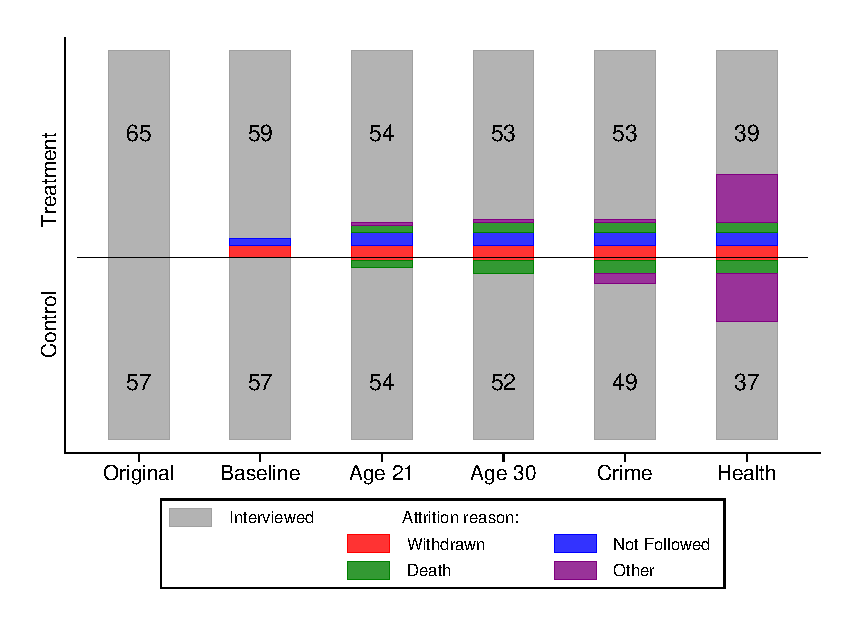
\includegraphics[width=.9\columnwidth]{output/abc_attrition.eps}
  \floatfoot{
\footnotesize
Note: This plot shows the number of participants in ABC for whom there exists data at the periods of data collection by experimental group. The children who withdrew from the study did so due to several reasons, such as adoption. Children were not followed if they were found to be biologically retarded after randomization. The numbers in the bars indicate the number of individuals who were interviewed during that phase of data collection. The original sample was measured after randomization but before the start of the program, the baseline sample was measured at the start of the program, and the health sample was collected at age 34.
}
\end{figure}
\end{comment}

\noindent Attrition was low in ABC. Information is available on 100 subjects in the age 30 follow-up, which we call the adult follow-up. In addition, 80 subjects---40 from the control group and 40 from the treatment group---consented to the release of their criminal records. Further, 70 participants consented to the release of information regarding a full-range biomedical panel---31 from the control group and 39 from the treatment group. \\

\noindent Attrition was also low for CARE subjects. Information is available on 58 subjects (more than 85\% of the initial sample) in the age-30 follow-up. Additionally, 40 participants (11 from the control group, 18 from the family education group, and 11 from the center-based childcare and family education group) released information on the full-range biomedical sweep. Administrative crime data are not available for CARE. We do not evaluate the second-phase of treatment in CARE because it was not randomized.  Rather, those in the center-based childcare and family education group and the family education group were offered school-age treatment, and those in the control group were not. \\

\noindent In the following set of tables (Table~\ref{tab:abc_baseline} through Table~\ref{tab:health_baseline}), we compare the observed, baseline characteristics between the first-phase control and treatment groups in ABC, which are the main groups we analyze, at different stages of the data collection follow-ups. For each observed characteristic, we present the bootstrapped $p$-value associated with the standard $t$-test. We also present the bootstrapped, step-down $p$-value on jointly testing the difference in observed characteristics across the two blocks of variables separated by the horizontal line.\footnote{\citet{Lehmann_Romano_2005_testing}.}\\

\noindent First, we compare the first-phase treatment and control groups on baseline characteristics.

\begin{table}[H]
\captionsetup{singlelinecheck=false,justification=centering}
\caption{First-phase Treatment vs. Control Groups \label{tab:baseline}}

  \begin{threeparttable}
  \begin{tabular}{cccccccc}
  \hline\hline

     &  & \scriptsize{Control} & \scriptsize{Treatment} & \scriptsize{Control} & \scriptsize{Treatment} & \mc{2}{c}{\scriptsize{$p$-value}} \\  

    \scriptsize{Variable} & \scriptsize{Age} & \scriptsize{Obs.} & \scriptsize{Obs.} & \scriptsize{Mean} & \scriptsize{Mean} & \scriptsize{Single $H_0$} & \scriptsize{Multiple $H_0$} \\ 
    \hline  

    \mc{1}{l}{\scriptsize{Male}} & \mc{1}{c}{\scriptsize{0}} & \mc{1}{c}{\scriptsize{57}} & \mc{1}{c}{\scriptsize{59}} & \mc{1}{c}{\scriptsize{0.438}} & \mc{1}{c}{\scriptsize{0.489}} & \mc{1}{c}{\scriptsize{(0.580)}} & \mc{1}{c}{\scriptsize{(0.700)}} \\  

    \mc{1}{l}{\scriptsize{Birth Weight}} & \mc{1}{c}{\scriptsize{0}} & \mc{1}{c}{\scriptsize{56}} & \mc{1}{c}{\scriptsize{58}} & \mc{1}{c}{\scriptsize{7.191}} & \mc{1}{c}{\scriptsize{6.829}} & \mc{1}{c}{\scriptsize{(0.130)}} & \mc{1}{c}{\scriptsize{(0.205)}} \\  

    \mc{1}{l}{\scriptsize{No. Siblings in Household}} & \mc{1}{c}{\scriptsize{0}} & \mc{1}{c}{\scriptsize{57}} & \mc{1}{c}{\scriptsize{59}} & \mc{1}{c}{\scriptsize{0.750}} & \mc{1}{c}{\scriptsize{0.516}} & \mc{1}{c}{\scriptsize{(0.245)}} & \mc{1}{c}{\scriptsize{(0.425)}} \\  

    \mc{1}{l}{\scriptsize{Birth Year}} & \mc{1}{c}{\scriptsize{0}} & \mc{1}{c}{\scriptsize{57}} & \mc{1}{c}{\scriptsize{59}} & \mc{1}{c}{\scriptsize{1974}} & \mc{1}{c}{\scriptsize{1974}} & \mc{1}{c}{\scriptsize{(0.785)}} & \mc{1}{c}{\scriptsize{(0.865)}} \\ 
    \hline  

    \mc{1}{l}{\scriptsize{Mother's Education}} & \mc{1}{c}{\scriptsize{0}} & \mc{1}{c}{\scriptsize{57}} & \mc{1}{c}{\scriptsize{59}} & \mc{1}{c}{\scriptsize{9.864}} & \mc{1}{c}{\scriptsize{10.505}} & \mc{1}{c}{\scriptsize{\textbf{(0.050)}}} & \mc{1}{c}{\scriptsize{\textbf{(0.090)}}} \\  

    \mc{1}{l}{\scriptsize{Mother's Age}} & \mc{1}{c}{\scriptsize{0}} & \mc{1}{c}{\scriptsize{57}} & \mc{1}{c}{\scriptsize{59}} & \mc{1}{c}{\scriptsize{20.103}} & \mc{1}{c}{\scriptsize{19.564}} & \mc{1}{c}{\scriptsize{(0.555)}} & \mc{1}{c}{\scriptsize{(0.665)}} \\  

    \mc{1}{l}{\scriptsize{Parental Income}} & \mc{1}{c}{\scriptsize{0}} & \mc{1}{c}{\scriptsize{57}} & \mc{1}{c}{\scriptsize{58}} & \mc{1}{c}{\scriptsize{6,211}} & \mc{1}{c}{\scriptsize{7,019}} & \mc{1}{c}{\scriptsize{(0.645)}} & \mc{1}{c}{\scriptsize{(0.720)}} \\  

    \mc{1}{l}{\scriptsize{Mother's IQ}} & \mc{1}{c}{\scriptsize{0}} & \mc{1}{c}{\scriptsize{57}} & \mc{1}{c}{\scriptsize{59}} & \mc{1}{c}{\scriptsize{83.419}} & \mc{1}{c}{\scriptsize{85.393}} & \mc{1}{c}{\scriptsize{(0.360)}} & \mc{1}{c}{\scriptsize{(0.510)}} \\  

    \mc{1}{l}{\scriptsize{Father at Home}} & \mc{1}{c}{\scriptsize{0}} & \mc{1}{c}{\scriptsize{57}} & \mc{1}{c}{\scriptsize{59}} & \mc{1}{c}{\scriptsize{0.346}} & \mc{1}{c}{\scriptsize{0.223}} & \mc{1}{c}{\scriptsize{(0.135)}} & \mc{1}{c}{\scriptsize{(0.270)}} \\  

  \hline\hline
  \end{tabular}
    \begin{tablenotes}
    \scriptsize
    \item 
    Note: This table shows the balance in observed characteristics between the treatment and control groups at baseline.
    For each characteristic, we present the $p$-value from a single hypothesis test.
    We also present the $p$-values from multiple testing, where we collectively test the
    baseline characteristics within the blocks separated by the horizontal line.
    Both $p$-values are two-sided and non-parametric. We construct them 
    based on 1,000 re-draws of the full sample. The estimates we display are the means of 
    the empirical bootstrap distribution. 
    
    \end{tablenotes}
  \end{threeparttable}

\end{table}

\noindent Second, we present the same exercise for each of the four cohorts ABC served.

\begin{table}[H]
\captionsetup{singlelinecheck=false,justification=centering}
\caption{First-phase Treatment vs. Control Groups, ABC Cohort 1 \label{tab:baseline_coh1}}

  \begin{threeparttable}
  \begin{tabular}{cccccccc}
  \toprule

     &  & \scriptsize{Control} & \scriptsize{Treated} & \scriptsize{Control} & \scriptsize{Treated} & \mc{2}{c}{\scriptsize{$p$-value}} \\  

    \scriptsize{Variable} & \scriptsize{Age} & \scriptsize{Obs.} & \scriptsize{Obs.} & \scriptsize{Mean} & \scriptsize{Mean} & \scriptsize{Single $H_0$} & \scriptsize{Multiple $H_0$} \\ 
    \midrule  

    \mc{1}{l}{\scriptsize{Male}} & \mc{1}{c}{\scriptsize{0}} & \mc{1}{c}{\scriptsize{14}} & \mc{1}{c}{\scriptsize{14}} & \mc{1}{c}{\scriptsize{0.348}} & \mc{1}{c}{\scriptsize{0.286}} & \mc{1}{c}{\scriptsize{(0.730)}} & \mc{1}{c}{\scriptsize{(0.738)}} \\  

    \mc{1}{l}{\scriptsize{Birth Weight}} & \mc{1}{c}{\scriptsize{0}} & \mc{1}{c}{\scriptsize{14}} & \mc{1}{c}{\scriptsize{13}} & \mc{1}{c}{\scriptsize{6.755}} & \mc{1}{c}{\scriptsize{6.491}} & \mc{1}{c}{\scriptsize{(0.550)}} & \mc{1}{c}{\scriptsize{(0.655)}} \\  

    \mc{1}{l}{\scriptsize{No. Siblings in Household}} & \mc{1}{c}{\scriptsize{0}} & \mc{1}{c}{\scriptsize{14}} & \mc{1}{c}{\scriptsize{14}} & \mc{1}{c}{\scriptsize{1.741}} & \mc{1}{c}{\scriptsize{0.606}} & \mc{1}{c}{\scriptsize{\textbf{(0.035)}}} & \mc{1}{c}{\scriptsize{\textbf{(0.085)}}} \\  

    \mc{1}{l}{\scriptsize{Birth Year}} & \mc{1}{c}{\scriptsize{0}} & \mc{1}{c}{\scriptsize{14}} & \mc{1}{c}{\scriptsize{14}} & \mc{1}{c}{\scriptsize{1972}} & \mc{1}{c}{\scriptsize{1972}} & \mc{1}{c}{\scriptsize{(0.240)}} & \mc{1}{c}{\scriptsize{(0.350)}} \\ 
    \midrule 

    \mc{1}{l}{\scriptsize{Mother's Education}} & \mc{1}{c}{\scriptsize{0}} & \mc{1}{c}{\scriptsize{14}} & \mc{1}{c}{\scriptsize{14}} & \mc{1}{c}{\scriptsize{9.885}} & \mc{1}{c}{\scriptsize{10.561}} & \mc{1}{c}{\scriptsize{(0.265)}} & \mc{1}{c}{\scriptsize{(0.480)}} \\  

    \mc{1}{l}{\scriptsize{Mother's Age}} & \mc{1}{c}{\scriptsize{0}} & \mc{1}{c}{\scriptsize{14}} & \mc{1}{c}{\scriptsize{14}} & \mc{1}{c}{\scriptsize{23.869}} & \mc{1}{c}{\scriptsize{19.552}} & \mc{1}{c}{\scriptsize{\textbf{(0.050)}}} & \mc{1}{c}{\scriptsize{(0.135)}} \\  

    \mc{1}{l}{\scriptsize{Mother Employed}} & \mc{1}{c}{\scriptsize{0}} & \mc{1}{c}{\scriptsize{14}} & \mc{1}{c}{\scriptsize{14}} & \mc{1}{c}{\scriptsize{0.152}} & \mc{1}{c}{\scriptsize{0.205}} & \mc{1}{c}{\scriptsize{(0.695)}} & \mc{1}{c}{\scriptsize{(0.895)}} \\  

    \mc{1}{l}{\scriptsize{Parental Income}} & \mc{1}{c}{\scriptsize{0}} & \mc{1}{c}{\scriptsize{14}} & \mc{1}{c}{\scriptsize{13}} & \mc{1}{c}{\scriptsize{7,164}} & \mc{1}{c}{\scriptsize{8,298}} & \mc{1}{c}{\scriptsize{(0.755)}} & \mc{1}{c}{\scriptsize{(0.910)}} \\  

    \mc{1}{l}{\scriptsize{Mother's IQ}} & \mc{1}{c}{\scriptsize{0}} & \mc{1}{c}{\scriptsize{14}} & \mc{1}{c}{\scriptsize{14}} & \mc{1}{c}{\scriptsize{76.042}} & \mc{1}{c}{\scriptsize{81.108}} & \mc{1}{c}{\scriptsize{(0.270)}} & \mc{1}{c}{\scriptsize{(0.485)}} \\  

    \mc{1}{l}{\scriptsize{Father at Home}} & \mc{1}{c}{\scriptsize{0}} & \mc{1}{c}{\scriptsize{14}} & \mc{1}{c}{\scriptsize{14}} & \mc{1}{c}{\scriptsize{0.559}} & \mc{1}{c}{\scriptsize{0.368}} & \mc{1}{c}{\scriptsize{(0.340)}} & \mc{1}{c}{\scriptsize{(0.493)}} \\  

  \bottomrule
  \end{tabular}
    \begin{tablenotes}
    \scriptsize
    \item 
    Note: This table shows the balance in observed characteristics between the treatment and control groups in ABC at baseline for cohort 1.
    For each characteristic, we present the $p$-value from a single hypothesis test.
    We also present the $p$-values from multiple hypothesis testing, where we collectively test the
    baseline characteristics within the blocks separated by the horizontal line.
    Both $p$-values are two-sided and non-parametric. We construct them 
    based on 200 re-draws of the full sample. The estimates we display are the means of 
    the empirical bootstrap distribution. 
    
    \end{tablenotes}
  \end{threeparttable}

\end{table}

\begin{table}[H]
\captionsetup{singlelinecheck=false,justification=centering}
\caption{First-phase Treatment vs. Control Groups, ABC Cohort 2 \label{tab:baseline_coh2}}

  \begin{threeparttable}
  \begin{tabular}{cccccccc}
  \toprule

     &  & \scriptsize{Control} & \scriptsize{Treated} & \scriptsize{Control} & \scriptsize{Treated} & \mc{2}{c}{\scriptsize{$p$-value}} \\  

    \scriptsize{Variable} & \scriptsize{Age} & \scriptsize{Obs.} & \scriptsize{Obs.} & \scriptsize{Mean} & \scriptsize{Mean} & \scriptsize{Single $H_0$} & \scriptsize{Multiple $H_0$} \\ 
    \midrule

    \mc{1}{l}{\scriptsize{Male}} & \mc{1}{c}{\scriptsize{0}} & \mc{1}{c}{\scriptsize{13}} & \mc{1}{c}{\scriptsize{16}} & \mc{1}{c}{\scriptsize{0.457}} & \mc{1}{c}{\scriptsize{0.503}} & \mc{1}{c}{\scriptsize{(0.805)}} & \mc{1}{c}{\scriptsize{(0.875)}} \\  

    \mc{1}{l}{\scriptsize{Birth Weight}} & \mc{1}{c}{\scriptsize{0}} & \mc{1}{c}{\scriptsize{13}} & \mc{1}{c}{\scriptsize{16}} & \mc{1}{c}{\scriptsize{7.256}} & \mc{1}{c}{\scriptsize{6.534}} & \mc{1}{c}{\scriptsize{(0.160)}} & \mc{1}{c}{\scriptsize{(0.270)}} \\  

    \mc{1}{l}{\scriptsize{No. Siblings in Household}} & \mc{1}{c}{\scriptsize{0}} & \mc{1}{c}{\scriptsize{13}} & \mc{1}{c}{\scriptsize{16}} & \mc{1}{c}{\scriptsize{0.388}} & \mc{1}{c}{\scriptsize{0.316}} & \mc{1}{c}{\scriptsize{(0.755)}} & \mc{1}{c}{\scriptsize{(0.835)}} \\  

    \mc{1}{l}{\scriptsize{Birth Year}} & \mc{1}{c}{\scriptsize{0}} & \mc{1}{c}{\scriptsize{13}} & \mc{1}{c}{\scriptsize{16}} & \mc{1}{c}{\scriptsize{1973}} & \mc{1}{c}{\scriptsize{1973}} & \mc{1}{c}{\scriptsize{(0.850)}} & \mc{1}{c}{\scriptsize{(0.925)}} \\ 
    \midrule  

    \mc{1}{l}{\scriptsize{Mother's Education}} & \mc{1}{c}{\scriptsize{0}} & \mc{1}{c}{\scriptsize{13}} & \mc{1}{c}{\scriptsize{16}} & \mc{1}{c}{\scriptsize{10.225}} & \mc{1}{c}{\scriptsize{10.307}} & \mc{1}{c}{\scriptsize{(0.885)}} & \mc{1}{c}{\scriptsize{(0.940)}} \\  

    \mc{1}{l}{\scriptsize{Mother's Age}} & \mc{1}{c}{\scriptsize{0}} & \mc{1}{c}{\scriptsize{13}} & \mc{1}{c}{\scriptsize{16}} & \mc{1}{c}{\scriptsize{18.446}} & \mc{1}{c}{\scriptsize{17.637}} & \mc{1}{c}{\scriptsize{(0.380)}} & \mc{1}{c}{\scriptsize{(0.630)}} \\  

    \mc{1}{l}{\scriptsize{Mother Employed}} & \mc{1}{c}{\scriptsize{0}} & \mc{1}{c}{\scriptsize{13}} & \mc{1}{c}{\scriptsize{16}} & \mc{1}{c}{\scriptsize{0.307}} & \mc{1}{c}{\scriptsize{0.248}} & \mc{1}{c}{\scriptsize{(0.690)}} & \mc{1}{c}{\scriptsize{(0.850)}} \\  

    \mc{1}{l}{\scriptsize{Parental Income}} & \mc{1}{c}{\scriptsize{0}} & \mc{1}{c}{\scriptsize{13}} & \mc{1}{c}{\scriptsize{16}} & \mc{1}{c}{\scriptsize{5,398}} & \mc{1}{c}{\scriptsize{4,427}} & \mc{1}{c}{\scriptsize{(0.790)}} & \mc{1}{c}{\scriptsize{(0.880)}} \\  

    \mc{1}{l}{\scriptsize{Mother's IQ}} & \mc{1}{c}{\scriptsize{0}} & \mc{1}{c}{\scriptsize{13}} & \mc{1}{c}{\scriptsize{16}} & \mc{1}{c}{\scriptsize{86.873}} & \mc{1}{c}{\scriptsize{85.597}} & \mc{1}{c}{\scriptsize{(0.730)}} & \mc{1}{c}{\scriptsize{(0.855)}} \\  

    \mc{1}{l}{\scriptsize{Father at Home}} & \mc{1}{c}{\scriptsize{0}} & \mc{1}{c}{\scriptsize{13}} & \mc{1}{c}{\scriptsize{16}} & \mc{1}{c}{\scriptsize{0.220}} & \mc{1}{c}{\scriptsize{0.183}} & \mc{1}{c}{\scriptsize{(0.790)}} & \mc{1}{c}{\scriptsize{(0.895)}} \\  

  \bottomrule
  \end{tabular}
    \begin{tablenotes}
    \scriptsize
    \item 
    Note: This table shows the balance in observed characteristics between the treatment and control groups in ABC at baseline for cohort 2.
    For each characteristic, we present the $p$-value from a single hypothesis test.
    We also present the $p$-values from multiple hypothesis testing, where we collectively test the
    baseline characteristics within the blocks separated by the horizontal line.
    Both $p$-values are two-sided and non-parametric. We construct them 
    based on 200 re-draws of the full sample.
    
    \end{tablenotes}
  \end{threeparttable}

\end{table}

\begin{table}[H]
\captionsetup{singlelinecheck=false,justification=centering}
\caption{First-phase Treatment vs. Control Groups, ABC Cohort 3 \label{tab:baseline_coh3}}

  \begin{threeparttable}
  \begin{tabular}{cccccccc}
  \toprule

     &  & \scriptsize{Control} & \scriptsize{Treated} & \scriptsize{Control} & \scriptsize{Treated} & \mc{2}{c}{\scriptsize{$p$-value}} \\  

    \scriptsize{Variable} & \scriptsize{Age} & \scriptsize{Obs.} & \scriptsize{Obs.} & \scriptsize{Mean} & \scriptsize{Mean} & \scriptsize{Single $H_0$} & \scriptsize{Multiple $H_0$} \\ 
    \midrule

    \mc{1}{l}{\scriptsize{Male}} & \mc{1}{c}{\scriptsize{0}} & \mc{1}{c}{\scriptsize{14}} & \mc{1}{c}{\scriptsize{15}} & \mc{1}{c}{\scriptsize{0.376}} & \mc{1}{c}{\scriptsize{0.596}} & \mc{1}{c}{\scriptsize{(0.265)}} & \mc{1}{c}{\scriptsize{(0.320)}} \\  

    \mc{1}{l}{\scriptsize{Birth Weight}} & \mc{1}{c}{\scriptsize{0}} & \mc{1}{c}{\scriptsize{14}} & \mc{1}{c}{\scriptsize{15}} & \mc{1}{c}{\scriptsize{7.424}} & \mc{1}{c}{\scriptsize{7.138}} & \mc{1}{c}{\scriptsize{(0.470)}} & \mc{1}{c}{\scriptsize{(0.730)}} \\  

    \mc{1}{l}{\scriptsize{No. Siblings in Household}} & \mc{1}{c}{\scriptsize{0}} & \mc{1}{c}{\scriptsize{14}} & \mc{1}{c}{\scriptsize{15}} & \mc{1}{c}{\scriptsize{0.423}} & \mc{1}{c}{\scriptsize{0.203}} & \mc{1}{c}{\scriptsize{(0.385)}} & \mc{1}{c}{\scriptsize{(0.645)}} \\  

    \mc{1}{l}{\scriptsize{Birth Year}} & \mc{1}{c}{\scriptsize{0}} & \mc{1}{c}{\scriptsize{14}} & \mc{1}{c}{\scriptsize{15}} & \mc{1}{c}{\scriptsize{1975}} & \mc{1}{c}{\scriptsize{1975}} & \mc{1}{c}{\scriptsize{(0.510)}} & \mc{1}{c}{\scriptsize{(0.520)}} \\ 
    \midrule

    \mc{1}{l}{\scriptsize{Mother's Education}} & \mc{1}{c}{\scriptsize{0}} & \mc{1}{c}{\scriptsize{14}} & \mc{1}{c}{\scriptsize{15}} & \mc{1}{c}{\scriptsize{10.133}} & \mc{1}{c}{\scriptsize{10.704}} & \mc{1}{c}{\scriptsize{(0.405)}} & \mc{1}{c}{\scriptsize{(0.595)}} \\  

    \mc{1}{l}{\scriptsize{Mother's Age}} & \mc{1}{c}{\scriptsize{0}} & \mc{1}{c}{\scriptsize{14}} & \mc{1}{c}{\scriptsize{15}} & \mc{1}{c}{\scriptsize{18.602}} & \mc{1}{c}{\scriptsize{19.558}} & \mc{1}{c}{\scriptsize{(0.355)}} & \mc{1}{c}{\scriptsize{(0.570)}} \\  

    \mc{1}{l}{\scriptsize{Mother Employed}} & \mc{1}{c}{\scriptsize{0}} & \mc{1}{c}{\scriptsize{14}} & \mc{1}{c}{\scriptsize{15}} & \mc{1}{c}{\scriptsize{0.162}} & \mc{1}{c}{\scriptsize{0.467}} & \mc{1}{c}{\scriptsize{\textbf{(0.070)}}} & \mc{1}{c}{\scriptsize{(0.155)}} \\  

    \mc{1}{l}{\scriptsize{Parental Income}} & \mc{1}{c}{\scriptsize{0}} & \mc{1}{c}{\scriptsize{14}} & \mc{1}{c}{\scriptsize{15}} & \mc{1}{c}{\scriptsize{7,034}} & \mc{1}{c}{\scriptsize{4,981}} & \mc{1}{c}{\scriptsize{(0.430)}} & \mc{1}{c}{\scriptsize{(0.675)}} \\  

    \mc{1}{l}{\scriptsize{Mother's IQ}} & \mc{1}{c}{\scriptsize{0}} & \mc{1}{c}{\scriptsize{14}} & \mc{1}{c}{\scriptsize{15}} & \mc{1}{c}{\scriptsize{85.590}} & \mc{1}{c}{\scriptsize{88.715}} & \mc{1}{c}{\scriptsize{(0.435)}} & \mc{1}{c}{\scriptsize{(0.610)}} \\  

    \mc{1}{l}{\scriptsize{Father at Home}} & \mc{1}{c}{\scriptsize{0}} & \mc{1}{c}{\scriptsize{14}} & \mc{1}{c}{\scriptsize{15}} & \mc{1}{c}{\scriptsize{0.424}} & \mc{1}{c}{\scriptsize{0.209}} & \mc{1}{c}{\scriptsize{(0.265)}} & \mc{1}{c}{\scriptsize{(0.425)}} \\  

  \bottomrule
  \end{tabular}
    \begin{tablenotes}
    \scriptsize
    \item 
    Note: This table shows the balance in observed characteristics between the treatment and control groups in ABC at baseline for cohort 3.
    For each characteristic, we present the $p$-value from a single hypothesis test.
    We also present the $p$-values from multiple hypothesis testing, where we collectively test the
    baseline characteristics within the blocks separated by the horizontal line.
    Both $p$-values are two-sided and non-parametric. We construct them 
    based on 200 re-draws of the full sample. The estimates we display are the means of 
    the empirical bootstrap distribution. 
    
    \end{tablenotes}
  \end{threeparttable}

\end{table}

\begin{table}[H]
\captionsetup{singlelinecheck=false,justification=centering}
\caption{First-phase Treatment vs. Control Groups, ABC Cohort 4 \label{tab:baseline_coh4}}

  \begin{threeparttable}
  \begin{tabular}{cccccccc}
  \toprule

     &  & \scriptsize{Control} & \scriptsize{Treated} & \scriptsize{Control} & \scriptsize{Treated} & \mc{2}{c}{\scriptsize{$p$-value}} \\  

    \scriptsize{Variable} & \scriptsize{Age} & \scriptsize{Obs.} & \scriptsize{Obs.} & \scriptsize{Mean} & \scriptsize{Mean} & \scriptsize{Single $H_0$} & \scriptsize{Multiple $H_0$} \\ 
    \midrule

    \mc{1}{l}{\scriptsize{Male}} & \mc{1}{c}{\scriptsize{0}} & \mc{1}{c}{\scriptsize{15}} & \mc{1}{c}{\scriptsize{14}} & \mc{1}{c}{\scriptsize{0.599}} & \mc{1}{c}{\scriptsize{0.567}} & \mc{1}{c}{\scriptsize{(0.870)}} & \mc{1}{c}{\scriptsize{(0.905)}} \\  

    \mc{1}{l}{\scriptsize{Birth Weight}} & \mc{1}{c}{\scriptsize{0}} & \mc{1}{c}{\scriptsize{15}} & \mc{1}{c}{\scriptsize{14}} & \mc{1}{c}{\scriptsize{7.321}} & \mc{1}{c}{\scriptsize{7.150}} & \mc{1}{c}{\scriptsize{(0.725)}} & \mc{1}{c}{\scriptsize{(0.840)}} \\  

    \mc{1}{l}{\scriptsize{No. Siblings in Household}} & \mc{1}{c}{\scriptsize{0}} & \mc{1}{c}{\scriptsize{15}} & \mc{1}{c}{\scriptsize{14}} & \mc{1}{c}{\scriptsize{0.490}} & \mc{1}{c}{\scriptsize{0.977}} & \mc{1}{c}{\scriptsize{(0.220)}} & \mc{1}{c}{\scriptsize{(0.380)}} \\  

    \mc{1}{l}{\scriptsize{Birth Year}} & \mc{1}{c}{\scriptsize{0}} & \mc{1}{c}{\scriptsize{15}} & \mc{1}{c}{\scriptsize{14}} & \mc{1}{c}{\scriptsize{1977}} & \mc{1}{c}{\scriptsize{1977}} & \mc{1}{c}{\scriptsize{(0.615)}} & \mc{1}{c}{\scriptsize{(0.728)}} \\ 
    \midrule

    \mc{1}{l}{\scriptsize{Mother's Education}} & \mc{1}{c}{\scriptsize{0}} & \mc{1}{c}{\scriptsize{15}} & \mc{1}{c}{\scriptsize{14}} & \mc{1}{c}{\scriptsize{9.530}} & \mc{1}{c}{\scriptsize{10.424}} & \mc{1}{c}{\scriptsize{(0.240)}} & \mc{1}{c}{\scriptsize{(0.410)}} \\  

    \mc{1}{l}{\scriptsize{Mother's Age}} & \mc{1}{c}{\scriptsize{0}} & \mc{1}{c}{\scriptsize{15}} & \mc{1}{c}{\scriptsize{14}} & \mc{1}{c}{\scriptsize{19.941}} & \mc{1}{c}{\scriptsize{21.712}} & \mc{1}{c}{\scriptsize{(0.320)}} & \mc{1}{c}{\scriptsize{(0.570)}} \\  

    \mc{1}{l}{\scriptsize{Mother Employed}} & \mc{1}{c}{\scriptsize{0}} & \mc{1}{c}{\scriptsize{15}} & \mc{1}{c}{\scriptsize{14}} & \mc{1}{c}{\scriptsize{0.260}} & \mc{1}{c}{\scriptsize{0.347}} & \mc{1}{c}{\scriptsize{(0.650)}} & \mc{1}{c}{\scriptsize{(0.840)}} \\  

    \mc{1}{l}{\scriptsize{Parental Income}} & \mc{1}{c}{\scriptsize{0}} & \mc{1}{c}{\scriptsize{15}} & \mc{1}{c}{\scriptsize{14}} & \mc{1}{c}{\scriptsize{5,827}} & \mc{1}{c}{\scriptsize{10,781}} & \mc{1}{c}{\scriptsize{\textbf{(0.065)}}} & \mc{1}{c}{\scriptsize{(0.135)}} \\  

    \mc{1}{l}{\scriptsize{Mother's IQ}} & \mc{1}{c}{\scriptsize{0}} & \mc{1}{c}{\scriptsize{15}} & \mc{1}{c}{\scriptsize{14}} & \mc{1}{c}{\scriptsize{85.561}} & \mc{1}{c}{\scriptsize{86.004}} & \mc{1}{c}{\scriptsize{(0.920)}} & \mc{1}{c}{\scriptsize{(0.960)}} \\  

    \mc{1}{l}{\scriptsize{Father at Home}} & \mc{1}{c}{\scriptsize{0}} & \mc{1}{c}{\scriptsize{15}} & \mc{1}{c}{\scriptsize{14}} & \mc{1}{c}{\scriptsize{0.208}} & \mc{1}{c}{\scriptsize{0.138}} & \mc{1}{c}{\scriptsize{(0.570)}} & \mc{1}{c}{\scriptsize{(0.777)}} \\  

  \bottomrule
  \end{tabular}
    \begin{tablenotes}
    \scriptsize
    \item 
    Note: This table shows the balance in observed characteristics between the treatment and control groups in ABC at baseline for cohort 4.
    For each characteristic, we present the $p$-value from a single hypothesis test.
    We also present the $p$-values from multiple hypothesis testing, where we collectively test the
    baseline characteristics within the blocks separated by the horizontal line.
    Both $p$-values are two-sided and non-parametric. We construct them 
    based on 200 re-draws of the full sample.
    
    \end{tablenotes}
  \end{threeparttable}

\end{table}

\noindent Third, we compare the second-phase treatment and control groups on baseline characteristics.

\begin{table}[H]
\captionsetup{singlelinecheck=false,justification=centering}
\caption{Second-phase Treatment vs. Control Groups \label{tab:baseline_sa}}

  \begin{threeparttable}
  \begin{tabular}{cccccccc}
  \hline\hline

     &  & \scriptsize{Control} & \scriptsize{Treatment} & \scriptsize{Control} & \scriptsize{Treatment} & \mc{2}{c}{\scriptsize{$p$-value}} \\  

    \scriptsize{Variable} & \scriptsize{Age} & \scriptsize{Obs.} & \scriptsize{Obs.} & \scriptsize{Mean} & \scriptsize{Mean} & \scriptsize{Single $H_0$} & \scriptsize{Multiple $H_0$} \\ 
    \hline  

    \mc{1}{l}{\scriptsize{Male}} & \mc{1}{c}{\scriptsize{0}} & \mc{1}{c}{\scriptsize{47}} & \mc{1}{c}{\scriptsize{48}} & \mc{1}{c}{\scriptsize{0.551}} & \mc{1}{c}{\scriptsize{0.460}} & \mc{1}{c}{\scriptsize{(0.420)}} & \mc{1}{c}{\scriptsize{(0.552)}} \\  

    \mc{1}{l}{\scriptsize{Birth Weight}} & \mc{1}{c}{\scriptsize{0}} & \mc{1}{c}{\scriptsize{47}} & \mc{1}{c}{\scriptsize{48}} & \mc{1}{c}{\scriptsize{7.084}} & \mc{1}{c}{\scriptsize{6.929}} & \mc{1}{c}{\scriptsize{(0.610)}} & \mc{1}{c}{\scriptsize{(0.700)}} \\  

    \mc{1}{l}{\scriptsize{No. Siblings in Household}} & \mc{1}{c}{\scriptsize{0}} & \mc{1}{c}{\scriptsize{47}} & \mc{1}{c}{\scriptsize{48}} & \mc{1}{c}{\scriptsize{0.748}} & \mc{1}{c}{\scriptsize{0.504}} & \mc{1}{c}{\scriptsize{(0.285)}} & \mc{1}{c}{\scriptsize{(0.445)}} \\  

    \mc{1}{l}{\scriptsize{Birth Year}} & \mc{1}{c}{\scriptsize{0}} & \mc{1}{c}{\scriptsize{47}} & \mc{1}{c}{\scriptsize{48}} & \mc{1}{c}{\scriptsize{1974}} & \mc{1}{c}{\scriptsize{1974}} & \mc{1}{c}{\scriptsize{(0.835)}} & \mc{1}{c}{\scriptsize{(0.915)}} \\ 
    \hline  

    \mc{1}{l}{\scriptsize{Mother's Education}} & \mc{1}{c}{\scriptsize{0}} & \mc{1}{c}{\scriptsize{47}} & \mc{1}{c}{\scriptsize{48}} & \mc{1}{c}{\scriptsize{10.150}} & \mc{1}{c}{\scriptsize{10.388}} & \mc{1}{c}{\scriptsize{(0.480)}} & \mc{1}{c}{\scriptsize{(0.685)}} \\  

    \mc{1}{l}{\scriptsize{Mother's Age}} & \mc{1}{c}{\scriptsize{0}} & \mc{1}{c}{\scriptsize{47}} & \mc{1}{c}{\scriptsize{48}} & \mc{1}{c}{\scriptsize{21.122}} & \mc{1}{c}{\scriptsize{18.884}} & \mc{1}{c}{\scriptsize{\textbf{(0.035)}}} & \mc{1}{c}{\scriptsize{\textbf{(0.065)}}} \\  

    \mc{1}{l}{\scriptsize{Parental Income}} & \mc{1}{c}{\scriptsize{0}} & \mc{1}{c}{\scriptsize{47}} & \mc{1}{c}{\scriptsize{48}} & \mc{1}{c}{\scriptsize{7,589}} & \mc{1}{c}{\scriptsize{6,714}} & \mc{1}{c}{\scriptsize{(0.625)}} & \mc{1}{c}{\scriptsize{(0.795)}} \\  

    \mc{1}{l}{\scriptsize{Mother's IQ}} & \mc{1}{c}{\scriptsize{0}} & \mc{1}{c}{\scriptsize{47}} & \mc{1}{c}{\scriptsize{48}} & \mc{1}{c}{\scriptsize{83.000}} & \mc{1}{c}{\scriptsize{85.831}} & \mc{1}{c}{\scriptsize{(0.185)}} & \mc{1}{c}{\scriptsize{(0.350)}} \\  

    \mc{1}{l}{\scriptsize{Father at Home}} & \mc{1}{c}{\scriptsize{0}} & \mc{1}{c}{\scriptsize{47}} & \mc{1}{c}{\scriptsize{48}} & \mc{1}{c}{\scriptsize{0.279}} & \mc{1}{c}{\scriptsize{0.287}} & \mc{1}{c}{\scriptsize{(0.920)}} & \mc{1}{c}{\scriptsize{(0.965)}} \\  

  \hline\hline
  \end{tabular}
    \begin{tablenotes}
    \scriptsize
    \item 
    Note: This table shows the balance in observed characteristics between the school-age treatment and control groups at baseline.
    For each characteristic, we present the $p$-value from a single hypothesis test.
    We also present the $p$-values from multiple testing, where we collectively test the
    baseline characteristics within the blocks separated by the horizontal line.
    Both $p$-values are two-sided and non-parametric. We construct them 
    based on 200 re-draws of the full sample. The estimates we display are the means of 
    the empirical bootstrap distribution. 
    
    \end{tablenotes}
  \end{threeparttable}

\end{table}

\noindent Fourth, we compare the observed, baseline characteristics of attrited and non-attrited subjects in the first-phase treatment assignment.

\begin{table}[H]
\captionsetup{singlelinecheck=false,justification=centering}
\caption{Observed vs. Attritted Children, ABC \label{tab:attrition_baseline}}

  \begin{threeparttable}
  \begin{tabular}{cccccccc}
  \toprule

     &  &  &  & \scriptsize{Observed} & \scriptsize{Attritted} & \mc{2}{c}{\scriptsize{$p$-value}} \\  

    \scriptsize{Variable} & \scriptsize{Age} & \scriptsize{Obs.} & \scriptsize{Att.} & \scriptsize{Mean} & \scriptsize{Mean} & \scriptsize{Single $H_0$} & \scriptsize{Multiple $H_0$} \\ 
    \midrule

    \mc{1}{l}{\scriptsize{Male}} & \mc{1}{c}{\scriptsize{0}} & \mc{1}{c}{\scriptsize{103}} & \mc{1}{c}{\scriptsize{13}} & \mc{1}{c}{\scriptsize{0.488}} & \mc{1}{c}{\scriptsize{0.248}} & \mc{1}{c}{\scriptsize{\textbf{(0.085)}}} & \mc{1}{c}{\scriptsize{(0.140)}} \\  

    \mc{1}{l}{\scriptsize{Birth Weight}} & \mc{1}{c}{\scriptsize{0}} & \mc{1}{c}{\scriptsize{103}} & \mc{1}{c}{\scriptsize{11}} & \mc{1}{c}{\scriptsize{7.014}} & \mc{1}{c}{\scriptsize{6.948}} & \mc{1}{c}{\scriptsize{(0.825)}} & \mc{1}{c}{\scriptsize{(0.875)}} \\  

    \mc{1}{l}{\scriptsize{No. Siblings in Household}} & \mc{1}{c}{\scriptsize{0}} & \mc{1}{c}{\scriptsize{103}} & \mc{1}{c}{\scriptsize{13}} & \mc{1}{c}{\scriptsize{0.609}} & \mc{1}{c}{\scriptsize{0.829}} & \mc{1}{c}{\scriptsize{(0.600)}} & \mc{1}{c}{\scriptsize{(0.705)}} \\  

    \mc{1}{l}{\scriptsize{Birth Year}} & \mc{1}{c}{\scriptsize{0}} & \mc{1}{c}{\scriptsize{103}} & \mc{1}{c}{\scriptsize{13}} & \mc{1}{c}{\scriptsize{1974}} & \mc{1}{c}{\scriptsize{1973}} & \mc{1}{c}{\scriptsize{\textbf{(0.045)}}} & \mc{1}{c}{\scriptsize{\textbf{(0.095)}}} \\ 
    \midrule

    \mc{1}{l}{\scriptsize{Mother's Education}} & \mc{1}{c}{\scriptsize{0}} & \mc{1}{c}{\scriptsize{103}} & \mc{1}{c}{\scriptsize{13}} & \mc{1}{c}{\scriptsize{10.302}} & \mc{1}{c}{\scriptsize{9.192}} & \mc{1}{c}{\scriptsize{\textbf{(0.100)}}} & \mc{1}{c}{\scriptsize{(0.165)}} \\  

    \mc{1}{l}{\scriptsize{Mother's Age}} & \mc{1}{c}{\scriptsize{0}} & \mc{1}{c}{\scriptsize{103}} & \mc{1}{c}{\scriptsize{13}} & \mc{1}{c}{\scriptsize{20.016}} & \mc{1}{c}{\scriptsize{18.178}} & \mc{1}{c}{\scriptsize{\textbf{(0.080)}}} & \mc{1}{c}{\scriptsize{(0.160)}} \\  

    \mc{1}{l}{\scriptsize{Mother Employed}} & \mc{1}{c}{\scriptsize{0}} & \mc{1}{c}{\scriptsize{103}} & \mc{1}{c}{\scriptsize{13}} & \mc{1}{c}{\scriptsize{0.268}} & \mc{1}{c}{\scriptsize{0.255}} & \mc{1}{c}{\scriptsize{(0.925)}} & \mc{1}{c}{\scriptsize{(0.955)}} \\  

    \mc{1}{l}{\scriptsize{Parental Income}} & \mc{1}{c}{\scriptsize{0}} & \mc{1}{c}{\scriptsize{103}} & \mc{1}{c}{\scriptsize{12}} & \mc{1}{c}{\scriptsize{6,622}} & \mc{1}{c}{\scriptsize{6,442}} & \mc{1}{c}{\scriptsize{(0.950)}} & \mc{1}{c}{\scriptsize{(0.960)}} \\  

    \mc{1}{l}{\scriptsize{Mother's IQ}} & \mc{1}{c}{\scriptsize{0}} & \mc{1}{c}{\scriptsize{103}} & \mc{1}{c}{\scriptsize{13}} & \mc{1}{c}{\scriptsize{85.050}} & \mc{1}{c}{\scriptsize{78.834}} & \mc{1}{c}{\scriptsize{\textbf{(0.070)}}} & \mc{1}{c}{\scriptsize{(0.135)}} \\  

    \mc{1}{l}{\scriptsize{Father at Home}} & \mc{1}{c}{\scriptsize{0}} & \mc{1}{c}{\scriptsize{103}} & \mc{1}{c}{\scriptsize{13}} & \mc{1}{c}{\scriptsize{0.278}} & \mc{1}{c}{\scriptsize{0.329}} & \mc{1}{c}{\scriptsize{(0.735)}} & \mc{1}{c}{\scriptsize{(0.835)}} \\  

  \bottomrule
  \end{tabular}
    \begin{tablenotes}
    \scriptsize
    \item 
    Note: This table shows the balance in observed characteristics between ABC subjects who were followed up to at least age 21 and ABC subjects who attrited before age 21.
    For each characteristic, we present the $p$-value from a single hypothesis test.
    We also present the $p$-values from multiple hypothesis testing, where we collectively test the
    baseline characteristics within the blocks separated by the horizontal line.
    Both $p$-values are two-sided and non-parametric. We construct them 
    based on 200 re-draws of the full sample. The estimates we display are the means of 
    the empirical bootstrap distribution. 
    
    \end{tablenotes}
  \end{threeparttable}

\end{table}

\noindent Fifth, we compare the observed, baseline characteristics between the subjects in the treatment and the control groups, excluding those who did not comply to treatment.

\begin{table}[H]
\captionsetup{singlelinecheck=false,justification=centering}
\caption{First-stage Treatment vs. Control Groups, Dropping Attrited Children \label{tab:postattrition_baseline}}

  \begin{threeparttable}
  \begin{tabular}{cccccccc}
  \hline\hline

     &  & \scriptsize{Control} & \scriptsize{Treatment} & \scriptsize{Control} & \scriptsize{Treatment} & \mc{2}{c}{\scriptsize{$p$-value}} \\  

    \scriptsize{Variable} & \scriptsize{Age} & \scriptsize{Obs.} & \scriptsize{Obs.} & \scriptsize{Mean} & \scriptsize{Mean} & \scriptsize{Single $H_0$} & \scriptsize{Multiple $H_0$} \\ 
    \hline  

    \mc{1}{l}{\scriptsize{Male}} & \mc{1}{c}{\scriptsize{0}} & \mc{1}{c}{\scriptsize{51}} & \mc{1}{c}{\scriptsize{52}} & \mc{1}{c}{\scriptsize{0.452}} & \mc{1}{c}{\scriptsize{0.524}} & \mc{1}{c}{\scriptsize{(0.430)}} & \mc{1}{c}{\scriptsize{(0.600)}} \\  

    \mc{1}{l}{\scriptsize{Birth Weight}} & \mc{1}{c}{\scriptsize{0}} & \mc{1}{c}{\scriptsize{51}} & \mc{1}{c}{\scriptsize{52}} & \mc{1}{c}{\scriptsize{7.210}} & \mc{1}{c}{\scriptsize{6.822}} & \mc{1}{c}{\scriptsize{(0.115)}} & \mc{1}{c}{\scriptsize{(0.220)}} \\  

    \mc{1}{l}{\scriptsize{No. Siblings in Household}} & \mc{1}{c}{\scriptsize{0}} & \mc{1}{c}{\scriptsize{51}} & \mc{1}{c}{\scriptsize{52}} & \mc{1}{c}{\scriptsize{0.767}} & \mc{1}{c}{\scriptsize{0.455}} & \mc{1}{c}{\scriptsize{(0.150)}} & \mc{1}{c}{\scriptsize{(0.230)}} \\  

    \mc{1}{l}{\scriptsize{Birth Year}} & \mc{1}{c}{\scriptsize{0}} & \mc{1}{c}{\scriptsize{51}} & \mc{1}{c}{\scriptsize{52}} & \mc{1}{c}{\scriptsize{1974}} & \mc{1}{c}{\scriptsize{1974}} & \mc{1}{c}{\scriptsize{(0.635)}} & \mc{1}{c}{\scriptsize{(0.785)}} \\ 
    \hline  

    \mc{1}{l}{\scriptsize{Mother's Education}} & \mc{1}{c}{\scriptsize{0}} & \mc{1}{c}{\scriptsize{51}} & \mc{1}{c}{\scriptsize{52}} & \mc{1}{c}{\scriptsize{10.000}} & \mc{1}{c}{\scriptsize{10.598}} & \mc{1}{c}{\scriptsize{\textbf{(0.085)}}} & \mc{1}{c}{\scriptsize{(0.160)}} \\  

    \mc{1}{l}{\scriptsize{Mother's Age}} & \mc{1}{c}{\scriptsize{0}} & \mc{1}{c}{\scriptsize{51}} & \mc{1}{c}{\scriptsize{52}} & \mc{1}{c}{\scriptsize{20.412}} & \mc{1}{c}{\scriptsize{19.635}} & \mc{1}{c}{\scriptsize{(0.405)}} & \mc{1}{c}{\scriptsize{(0.580)}} \\  

    \mc{1}{l}{\scriptsize{Parental Income}} & \mc{1}{c}{\scriptsize{0}} & \mc{1}{c}{\scriptsize{51}} & \mc{1}{c}{\scriptsize{52}} & \mc{1}{c}{\scriptsize{6,409}} & \mc{1}{c}{\scriptsize{6,846}} & \mc{1}{c}{\scriptsize{(0.765)}} & \mc{1}{c}{\scriptsize{(0.835)}} \\  

    \mc{1}{l}{\scriptsize{Mother's IQ}} & \mc{1}{c}{\scriptsize{0}} & \mc{1}{c}{\scriptsize{51}} & \mc{1}{c}{\scriptsize{52}} & \mc{1}{c}{\scriptsize{84.472}} & \mc{1}{c}{\scriptsize{85.635}} & \mc{1}{c}{\scriptsize{(0.560)}} & \mc{1}{c}{\scriptsize{(0.715)}} \\  

    \mc{1}{l}{\scriptsize{Father at Home}} & \mc{1}{c}{\scriptsize{0}} & \mc{1}{c}{\scriptsize{51}} & \mc{1}{c}{\scriptsize{52}} & \mc{1}{c}{\scriptsize{0.349}} & \mc{1}{c}{\scriptsize{0.208}} & \mc{1}{c}{\scriptsize{(0.115)}} & \mc{1}{c}{\scriptsize{(0.225)}} \\  

  \hline\hline
  \end{tabular}
    \begin{tablenotes}
    \scriptsize
    \item 
    Note: This table shows the balance in observed characteristics between the treatment and control groups of subjects who were followed up to at least age 21.
    For each characteristic, we present the $p$-value from a single hypothesis test.
    We also present the $p$-values from multiple testing, where we collectively test the
    baseline characteristics within the blocks separated by the horizontal line.
    Both $p$-values are two-sided and non-parametric. We construct them 
    based on 1,000 re-draws of the full sample. The estimates we display are the means of 
    the empirical bootstrap distribution. 
    
    \end{tablenotes}
  \end{threeparttable}

\end{table}

% AZ: commenting out until we get the CORRECT numbers
\begin{comment}
\noindent Sixth, we compare the observed baseline characteristics between the subjects in the first-phase treatment, restricting the sample to those who consented to release their age-34 criminal records.

\begin{table}[H]
\captionsetup{singlelinecheck=false,justification=centering}
\caption{First-phase Treatment vs. Control Groups, Children who Released Criminal Records, ABC \label{tab:crime_baseline}}

  \begin{threeparttable}
  \begin{tabular}{cccccccc}
  \hline\hline

     &  & \scriptsize{Control} & \scriptsize{Treated} & \scriptsize{Control} & \scriptsize{Treated} & \mc{2}{c}{\scriptsize{$p$-value}} \\  

    \scriptsize{Variable} & \scriptsize{Age} & \scriptsize{Obs.} & \scriptsize{Obs.} & \scriptsize{Mean} & \scriptsize{Mean} & \scriptsize{Single $H_0$} & \scriptsize{Multiple $H_0$} \\ 
    \hline  

    \mc{1}{l}{\scriptsize{Male}} & \mc{1}{c}{\scriptsize{0}} & \mc{1}{c}{\scriptsize{45}} & \mc{1}{c}{\scriptsize{43}} & \mc{1}{c}{\scriptsize{0.423}} & \mc{1}{c}{\scriptsize{0.527}} & \mc{1}{c}{\scriptsize{(0.275)}} & \mc{1}{c}{\scriptsize{(0.425)}} \\  

    \mc{1}{l}{\scriptsize{Birth Weight}} & \mc{1}{c}{\scriptsize{0}} & \mc{1}{c}{\scriptsize{45}} & \mc{1}{c}{\scriptsize{43}} & \mc{1}{c}{\scriptsize{7.226}} & \mc{1}{c}{\scriptsize{6.940}} & \mc{1}{c}{\scriptsize{(0.295)}} & \mc{1}{c}{\scriptsize{(0.415)}} \\  

    \mc{1}{l}{\scriptsize{No. Siblings in Household}} & \mc{1}{c}{\scriptsize{0}} & \mc{1}{c}{\scriptsize{45}} & \mc{1}{c}{\scriptsize{43}} & \mc{1}{c}{\scriptsize{0.780}} & \mc{1}{c}{\scriptsize{0.491}} & \mc{1}{c}{\scriptsize{(0.220)}} & \mc{1}{c}{\scriptsize{(0.340)}} \\  

    \mc{1}{l}{\scriptsize{Birth Year}} & \mc{1}{c}{\scriptsize{0}} & \mc{1}{c}{\scriptsize{45}} & \mc{1}{c}{\scriptsize{43}} & \mc{1}{c}{\scriptsize{1975}} & \mc{1}{c}{\scriptsize{1974}} & \mc{1}{c}{\scriptsize{(0.520)}} & \mc{1}{c}{\scriptsize{(0.680)}} \\ 
    \hline  

    \mc{1}{l}{\scriptsize{Mother's Education}} & \mc{1}{c}{\scriptsize{0}} & \mc{1}{c}{\scriptsize{45}} & \mc{1}{c}{\scriptsize{43}} & \mc{1}{c}{\scriptsize{9.947}} & \mc{1}{c}{\scriptsize{10.485}} & \mc{1}{c}{\scriptsize{(0.125)}} & \mc{1}{c}{\scriptsize{(0.235)}} \\  

    \mc{1}{l}{\scriptsize{Mother's Age}} & \mc{1}{c}{\scriptsize{0}} & \mc{1}{c}{\scriptsize{45}} & \mc{1}{c}{\scriptsize{43}} & \mc{1}{c}{\scriptsize{20.273}} & \mc{1}{c}{\scriptsize{19.571}} & \mc{1}{c}{\scriptsize{(0.530)}} & \mc{1}{c}{\scriptsize{(0.725)}} \\  

    \mc{1}{l}{\scriptsize{Mother Employed}} & \mc{1}{c}{\scriptsize{0}} & \mc{1}{c}{\scriptsize{45}} & \mc{1}{c}{\scriptsize{43}} & \mc{1}{c}{\scriptsize{0.199}} & \mc{1}{c}{\scriptsize{0.318}} & \mc{1}{c}{\scriptsize{(0.195)}} & \mc{1}{c}{\scriptsize{(0.415)}} \\  

    \mc{1}{l}{\scriptsize{Parental Income}} & \mc{1}{c}{\scriptsize{0}} & \mc{1}{c}{\scriptsize{45}} & \mc{1}{c}{\scriptsize{43}} & \mc{1}{c}{\scriptsize{5,751}} & \mc{1}{c}{\scriptsize{7,437}} & \mc{1}{c}{\scriptsize{(0.355)}} & \mc{1}{c}{\scriptsize{(0.565)}} \\  

    \mc{1}{l}{\scriptsize{Mother's IQ}} & \mc{1}{c}{\scriptsize{0}} & \mc{1}{c}{\scriptsize{45}} & \mc{1}{c}{\scriptsize{43}} & \mc{1}{c}{\scriptsize{84.612}} & \mc{1}{c}{\scriptsize{85.504}} & \mc{1}{c}{\scriptsize{(0.655)}} & \mc{1}{c}{\scriptsize{(0.840)}} \\  

    \mc{1}{l}{\scriptsize{Father at Home}} & \mc{1}{c}{\scriptsize{0}} & \mc{1}{c}{\scriptsize{45}} & \mc{1}{c}{\scriptsize{43}} & \mc{1}{c}{\scriptsize{0.334}} & \mc{1}{c}{\scriptsize{0.256}} & \mc{1}{c}{\scriptsize{(0.390)}} & \mc{1}{c}{\scriptsize{(0.635)}} \\  

  \hline\hline
  \end{tabular}
    \begin{tablenotes}
    \scriptsize
    \item 
    Note: This table shows the balance in observed characteristics between the treatment and control groups in ABC at baseline for subjects who consented to release their administrative criminal records.
    For each characteristic, we present the $p$-value from a single hypothesis test.
    We also present the $p$-values from multiple testing, where we collectively test the
    baseline characteristics within the blocks separated by the horizontal line.
    Both $p$-values are two-sided and non-parametric. We construct them 
    based on 200 re-draws of the full sample. The estimates we display are the means of 
    the empirical bootstrap distribution. 
    
    \end{tablenotes}
  \end{threeparttable}

\end{table}
\end{comment}

\noindent Finally, we compare the observed, baseline characteristics between the children in the first-phase treatment, restricting the sample to the children for whom we have information on the age-34 medical data collection.

\begin{table}[H]
\captionsetup{singlelinecheck=false,justification=centering}
\caption{First-phase Treatment vs. Control Groups, Children who Completed the Medical Sweep Follow-up, ABC \label{tab:health_baseline}}

  \begin{threeparttable}
  \begin{tabular}{cccccccc}
  \hline\hline

     &  & \scriptsize{Control} & \scriptsize{Treated} & \scriptsize{Control} & \scriptsize{Treated} & \mc{2}{c}{\scriptsize{$p$-value}} \\  

    \scriptsize{Variable} & \scriptsize{Age} & \scriptsize{Obs.} & \scriptsize{Obs.} & \scriptsize{Mean} & \scriptsize{Mean} & \scriptsize{Single $H_0$} & \scriptsize{Multiple $H_0$} \\ 
    \hline  

    \mc{1}{l}{\scriptsize{Male}} & \mc{1}{c}{\scriptsize{0}} & \mc{1}{c}{\scriptsize{31}} & \mc{1}{c}{\scriptsize{39}} & \mc{1}{c}{\scriptsize{0.293}} & \mc{1}{c}{\scriptsize{0.533}} & \mc{1}{c}{\scriptsize{\textbf{(0.050)}}} & \mc{1}{c}{\scriptsize{\textbf{(0.055)}}} \\  

    \mc{1}{l}{\scriptsize{Birth Weight}} & \mc{1}{c}{\scriptsize{0}} & \mc{1}{c}{\scriptsize{31}} & \mc{1}{c}{\scriptsize{39}} & \mc{1}{c}{\scriptsize{7.233}} & \mc{1}{c}{\scriptsize{6.826}} & \mc{1}{c}{\scriptsize{(0.190)}} & \mc{1}{c}{\scriptsize{(0.295)}} \\  

    \mc{1}{l}{\scriptsize{No. Siblings in Household}} & \mc{1}{c}{\scriptsize{0}} & \mc{1}{c}{\scriptsize{31}} & \mc{1}{c}{\scriptsize{39}} & \mc{1}{c}{\scriptsize{0.613}} & \mc{1}{c}{\scriptsize{0.493}} & \mc{1}{c}{\scriptsize{(0.580)}} & \mc{1}{c}{\scriptsize{(0.750)}} \\  

    \mc{1}{l}{\scriptsize{Birth Year}} & \mc{1}{c}{\scriptsize{0}} & \mc{1}{c}{\scriptsize{31}} & \mc{1}{c}{\scriptsize{39}} & \mc{1}{c}{\scriptsize{1975}} & \mc{1}{c}{\scriptsize{1974}} & \mc{1}{c}{\scriptsize{(0.360)}} & \mc{1}{c}{\scriptsize{(0.510)}} \\ 
    \hline  

    \mc{1}{l}{\scriptsize{Mother's Education}} & \mc{1}{c}{\scriptsize{0}} & \mc{1}{c}{\scriptsize{31}} & \mc{1}{c}{\scriptsize{39}} & \mc{1}{c}{\scriptsize{10.039}} & \mc{1}{c}{\scriptsize{10.597}} & \mc{1}{c}{\scriptsize{(0.190)}} & \mc{1}{c}{\scriptsize{(0.385)}} \\  

    \mc{1}{l}{\scriptsize{Mother's Age}} & \mc{1}{c}{\scriptsize{0}} & \mc{1}{c}{\scriptsize{31}} & \mc{1}{c}{\scriptsize{39}} & \mc{1}{c}{\scriptsize{19.389}} & \mc{1}{c}{\scriptsize{19.595}} & \mc{1}{c}{\scriptsize{(0.825)}} & \mc{1}{c}{\scriptsize{(0.945)}} \\  

    \mc{1}{l}{\scriptsize{Mother Employed}} & \mc{1}{c}{\scriptsize{0}} & \mc{1}{c}{\scriptsize{31}} & \mc{1}{c}{\scriptsize{39}} & \mc{1}{c}{\scriptsize{0.195}} & \mc{1}{c}{\scriptsize{0.349}} & \mc{1}{c}{\scriptsize{(0.185)}} & \mc{1}{c}{\scriptsize{(0.315)}} \\  

    \mc{1}{l}{\scriptsize{Parental Income}} & \mc{1}{c}{\scriptsize{0}} & \mc{1}{c}{\scriptsize{31}} & \mc{1}{c}{\scriptsize{39}} & \mc{1}{c}{\scriptsize{5,509}} & \mc{1}{c}{\scriptsize{7,520}} & \mc{1}{c}{\scriptsize{(0.280)}} & \mc{1}{c}{\scriptsize{(0.535)}} \\  

    \mc{1}{l}{\scriptsize{Mother's IQ}} & \mc{1}{c}{\scriptsize{0}} & \mc{1}{c}{\scriptsize{31}} & \mc{1}{c}{\scriptsize{39}} & \mc{1}{c}{\scriptsize{83.822}} & \mc{1}{c}{\scriptsize{84.922}} & \mc{1}{c}{\scriptsize{(0.655)}} & \mc{1}{c}{\scriptsize{(0.860)}} \\  

    \mc{1}{l}{\scriptsize{Father at Home}} & \mc{1}{c}{\scriptsize{0}} & \mc{1}{c}{\scriptsize{31}} & \mc{1}{c}{\scriptsize{39}} & \mc{1}{c}{\scriptsize{0.355}} & \mc{1}{c}{\scriptsize{0.231}} & \mc{1}{c}{\scriptsize{(0.205)}} & \mc{1}{c}{\scriptsize{(0.450)}} \\  

  \hline\hline
  \end{tabular}
    \begin{tablenotes}
    \scriptsize
    \item 
    Note: This table shows the balance in observed characteristics between the treatment and control groups in ABC at baseline for subjects who completed the health follow-up at age 34.
    For each characteristic, we present the $p$-value from a single hypothesis test.
    We also present the $p$-values from multiple testing, where we collectively test the
    baseline characteristics within the blocks separated by the horizontal line.
    Both $p$-values are two-sided and non-parametric. We construct them 
    based on 200 re-draws of the full sample. The estimates we display are the means of 
    the empirical bootstrap distribution. 
    
    \end{tablenotes}
  \end{threeparttable}

\end{table}

\noindent Despite some exceptions, these tables indicate balance between the treatment and control groups from the first-phase randomization, which is the primary comparison we analyze in the main paper. The balance in observed characteristics holds for the different samples we consider, which differs from the initial sample due to various instances of item non-response. For the second-phase randomization, there is also balance in observed characteristics. \\

\noindent Table \ref{tab:care_baseline2} through Table \ref{tab:health_baseline_care_t1} are the analogous tables for CARE. We compare the two treatment groups (center-based childcare and family education, and only family education) separately across the full sample and by cohort. The inference statistics are constructed using the same methods as for Table \ref{tab:abc_baseline} through Table \ref{tab:health_baseline}. \\

\begin{table}[H]
\captionsetup{singlelinecheck=false,justification=centering}
\caption{CARE Baseline Characteristics, Control vs. Family Education and Center-based Childcare \label{tab:care_baseline2}}

  \begin{threeparttable}
  \begin{tabular}{cccccccc}
  \toprule

     &  & \scriptsize{Control} & \scriptsize{Treated} & \scriptsize{Control} & \scriptsize{Treated} & \mc{2}{c}{\scriptsize{$p$-value}} \\  

    \scriptsize{Variable} & \scriptsize{Age} & \scriptsize{Obs.} & \scriptsize{Obs.} & \scriptsize{Mean} & \scriptsize{Mean} & \scriptsize{Single $H_0$} & \scriptsize{Multiple $H_0$} \\ 
    \midrule  

    \mc{1}{l}{\scriptsize{Male}} & \mc{1}{c}{\scriptsize{0}} & \mc{1}{c}{\scriptsize{23}} & \mc{1}{c}{\scriptsize{17}} & \mc{1}{c}{\scriptsize{0.611}} & \mc{1}{c}{\scriptsize{0.524}} & \mc{1}{c}{\scriptsize{(0.565)}} & \mc{1}{c}{\scriptsize{(0.740)}} \\  

    \mc{1}{l}{\scriptsize{Birth Weight}} & \mc{1}{c}{\scriptsize{0}} & \mc{1}{c}{\scriptsize{23}} & \mc{1}{c}{\scriptsize{15}} & \mc{1}{c}{\scriptsize{7.102}} & \mc{1}{c}{\scriptsize{7.508}} & \mc{1}{c}{\scriptsize{(0.335)}} & \mc{1}{c}{\scriptsize{(0.515)}} \\  

    \mc{1}{l}{\scriptsize{No. Siblings in Household}} & \mc{1}{c}{\scriptsize{0}} & \mc{1}{c}{\scriptsize{23}} & \mc{1}{c}{\scriptsize{17}} & \mc{1}{c}{\scriptsize{0.619}} & \mc{1}{c}{\scriptsize{0.653}} & \mc{1}{c}{\scriptsize{(0.895)}} & \mc{1}{c}{\scriptsize{(0.945)}} \\  

    \mc{1}{l}{\scriptsize{Birth Year}} & \mc{1}{c}{\scriptsize{0}} & \mc{1}{c}{\scriptsize{23}} & \mc{1}{c}{\scriptsize{17}} & \mc{1}{c}{\scriptsize{1979}} & \mc{1}{c}{\scriptsize{1979}} & \mc{1}{c}{\scriptsize{(0.890)}} & \mc{1}{c}{\scriptsize{(0.920)}} \\ 
    \midrule  

    \mc{1}{l}{\scriptsize{Mother's Education}} & \mc{1}{c}{\scriptsize{0}} & \mc{1}{c}{\scriptsize{23}} & \mc{1}{c}{\scriptsize{17}} & \mc{1}{c}{\scriptsize{11.195}} & \mc{1}{c}{\scriptsize{10.693}} & \mc{1}{c}{\scriptsize{(0.390)}} & \mc{1}{c}{\scriptsize{(0.500)}} \\  

    \mc{1}{l}{\scriptsize{Mother's Age}} & \mc{1}{c}{\scriptsize{0}} & \mc{1}{c}{\scriptsize{23}} & \mc{1}{c}{\scriptsize{17}} & \mc{1}{c}{\scriptsize{21.636}} & \mc{1}{c}{\scriptsize{21.896}} & \mc{1}{c}{\scriptsize{(0.870)}} & \mc{1}{c}{\scriptsize{(0.915)}} \\  

    \mc{1}{l}{\scriptsize{Mother's IQ}} & \mc{1}{c}{\scriptsize{0}} & \mc{1}{c}{\scriptsize{23}} & \mc{1}{c}{\scriptsize{17}} & \mc{1}{c}{\scriptsize{87.584}} & \mc{1}{c}{\scriptsize{86.624}} & \mc{1}{c}{\scriptsize{(0.725)}} & \mc{1}{c}{\scriptsize{(0.825)}} \\  

    \mc{1}{l}{\scriptsize{Father at Home}} & \mc{1}{c}{\scriptsize{0}} & \mc{1}{c}{\scriptsize{23}} & \mc{1}{c}{\scriptsize{17}} & \mc{1}{c}{\scriptsize{0.127}} & \mc{1}{c}{\scriptsize{0.351}} & \mc{1}{c}{\scriptsize{\textbf{(0.095)}}} & \mc{1}{c}{\scriptsize{(0.175)}} \\  

  \bottomrule
  \end{tabular}
    \begin{tablenotes}
    \scriptsize
    \item 
    Note: This table shows the balance in observed characteristics between the treatment and control groups at baseline.
    For each characteristic, we present the $p$-value from a single hypothesis test.
    We also present the $p$-values from multiple hypothesis testing, where we collectively test the
    baseline characteristics within the blocks separated by the horizontal line.
    Both $p$-values are two-sided and non-parametric. We construct them 
    based on 200 re-draws of the full sample. The estimates we display are the means of 
    the empirical bootstrap distribution. 
    
    \end{tablenotes}
  \end{threeparttable}

\end{table}

\begin{table}[H]
\captionsetup{singlelinecheck=false,justification=centering}
\caption{CARE Baseline Characteristics, Control vs. Family Education \label{tab:baseline}}

  \begin{threeparttable}
  \begin{tabular}{cccccccc}
  \toprule

     &  & \scriptsize{Control} & \scriptsize{Treated} & \scriptsize{Control} & \scriptsize{Treated} & \mc{2}{c}{\scriptsize{$p$-value}} \\  

    \scriptsize{Variable} & \scriptsize{Age} & \scriptsize{Obs.} & \scriptsize{Obs.} & \scriptsize{Mean} & \scriptsize{Mean} & \scriptsize{Single $H_0$} & \scriptsize{Multiple $H_0$} \\ 
    \midrule  

    \mc{1}{l}{\scriptsize{Male}} & \mc{1}{c}{\scriptsize{0}} & \mc{1}{c}{\scriptsize{23}} & \mc{1}{c}{\scriptsize{27}} & \mc{1}{c}{\scriptsize{0.611}} & \mc{1}{c}{\scriptsize{0.632}} & \mc{1}{c}{\scriptsize{(0.895)}} & \mc{1}{c}{\scriptsize{(0.880)}} \\  

    \mc{1}{l}{\scriptsize{Birth Weight}} & \mc{1}{c}{\scriptsize{0}} & \mc{1}{c}{\scriptsize{23}} & \mc{1}{c}{\scriptsize{26}} & \mc{1}{c}{\scriptsize{7.102}} & \mc{1}{c}{\scriptsize{6.963}} & \mc{1}{c}{\scriptsize{(0.755)}} & \mc{1}{c}{\scriptsize{(0.830)}} \\  

    \mc{1}{l}{\scriptsize{No. Siblings in Household}} & \mc{1}{c}{\scriptsize{0}} & \mc{1}{c}{\scriptsize{23}} & \mc{1}{c}{\scriptsize{27}} & \mc{1}{c}{\scriptsize{0.619}} & \mc{1}{c}{\scriptsize{0.758}} & \mc{1}{c}{\scriptsize{(0.680)}} & \mc{1}{c}{\scriptsize{(0.715)}} \\  

    \mc{1}{l}{\scriptsize{Birth Year}} & \mc{1}{c}{\scriptsize{0}} & \mc{1}{c}{\scriptsize{23}} & \mc{1}{c}{\scriptsize{27}} & \mc{1}{c}{\scriptsize{1979}} & \mc{1}{c}{\scriptsize{1979}} & \mc{1}{c}{\scriptsize{(0.330)}} & \mc{1}{c}{\scriptsize{(0.480)}} \\ 
    \midrule  

    \mc{1}{l}{\scriptsize{Mother's Education}} & \mc{1}{c}{\scriptsize{0}} & \mc{1}{c}{\scriptsize{23}} & \mc{1}{c}{\scriptsize{27}} & \mc{1}{c}{\scriptsize{11.195}} & \mc{1}{c}{\scriptsize{10.689}} & \mc{1}{c}{\scriptsize{(0.245)}} & \mc{1}{c}{\scriptsize{(0.380)}} \\  

    \mc{1}{l}{\scriptsize{Mother's Age}} & \mc{1}{c}{\scriptsize{0}} & \mc{1}{c}{\scriptsize{23}} & \mc{1}{c}{\scriptsize{27}} & \mc{1}{c}{\scriptsize{21.636}} & \mc{1}{c}{\scriptsize{20.257}} & \mc{1}{c}{\scriptsize{(0.305)}} & \mc{1}{c}{\scriptsize{(0.400)}} \\  

    \mc{1}{l}{\scriptsize{Mother's IQ}} & \mc{1}{c}{\scriptsize{0}} & \mc{1}{c}{\scriptsize{23}} & \mc{1}{c}{\scriptsize{27}} & \mc{1}{c}{\scriptsize{87.584}} & \mc{1}{c}{\scriptsize{87.167}} & \mc{1}{c}{\scriptsize{(0.855)}} & \mc{1}{c}{\scriptsize{(0.915)}} \\  

    \mc{1}{l}{\scriptsize{Father at Home}} & \mc{1}{c}{\scriptsize{0}} & \mc{1}{c}{\scriptsize{23}} & \mc{1}{c}{\scriptsize{27}} & \mc{1}{c}{\scriptsize{0.127}} & \mc{1}{c}{\scriptsize{0.190}} & \mc{1}{c}{\scriptsize{(0.455)}} & \mc{1}{c}{\scriptsize{(0.585)}} \\  

  \bottomrule
  \end{tabular}
    \begin{tablenotes}
    \scriptsize
    \item 
    Note: This table shows the balance in observed characteristics between the treatment and control groups at baseline.
    For each characteristic, we present the $p$-value from a single hypothesis test.
    We also present the $p$-values from multiple hypothesis testing, where we collectively test the
    baseline characteristics within the blocks separated by the horizontal line.
    Both $p$-values are two-sided and non-parametric. We construct them 
    based on 200 re-draws of the full sample. The estimates we display are the means of 
    the empirical bootstrap distribution. 
    
    \end{tablenotes}
  \end{threeparttable}

\end{table}

  \begin{tabular}{cccccccc}
  \toprule

     &  & \scriptsize{Control} & \scriptsize{Treated} & \scriptsize{Control} & \scriptsize{Treated} & \mc{2}{c}{\scriptsize{$p$-value}} \\  

    \scriptsize{Variable} & \scriptsize{Age} & \scriptsize{Obs.} & \scriptsize{Obs.} & \scriptsize{Mean} & \scriptsize{Mean} & \scriptsize{Single $H_0$} & \scriptsize{Multiple $H_0$} \\ 
    \midrule  

    \mc{1}{l}{\scriptsize{Male}} & \mc{1}{c}{\scriptsize{0}} & \mc{1}{c}{\scriptsize{7}} & \mc{1}{c}{\scriptsize{6}} & \mc{1}{c}{\scriptsize{0.571}} & \mc{1}{c}{\scriptsize{0.667}} & \mc{1}{c}{\scriptsize{(0.735)}} & \mc{1}{c}{\scriptsize{(0.865)}} \\  

    \mc{1}{l}{\scriptsize{Birth Weight}} & \mc{1}{c}{\scriptsize{0}} & \mc{1}{c}{\scriptsize{7}} & \mc{1}{c}{\scriptsize{4}} & \mc{1}{c}{\scriptsize{7.263}} & \mc{1}{c}{\scriptsize{7.485}} & \mc{1}{c}{\scriptsize{(0.678)}} & \mc{1}{c}{\scriptsize{(0.834)}} \\  

    \mc{1}{l}{\scriptsize{No. Siblings in Household}} & \mc{1}{c}{\scriptsize{0}} & \mc{1}{c}{\scriptsize{7}} & \mc{1}{c}{\scriptsize{6}} & \mc{1}{c}{\scriptsize{0.429}} & \mc{1}{c}{\scriptsize{0.500}} & \mc{1}{c}{\scriptsize{(0.866)}} & \mc{1}{c}{\scriptsize{(0.936)}} \\  

    \mc{1}{l}{\scriptsize{Birth Year}} & \mc{1}{c}{\scriptsize{0}} & \mc{1}{c}{\scriptsize{7}} & \mc{1}{c}{\scriptsize{6}} & \mc{1}{c}{\scriptsize{1978}} & \mc{1}{c}{\scriptsize{1978}} & \mc{1}{c}{\scriptsize{(0.551)}} & \mc{1}{c}{\scriptsize{(0.498)}} \\ 
    \midrule  

    \mc{1}{l}{\scriptsize{Mother's Education}} & \mc{1}{c}{\scriptsize{0}} & \mc{1}{c}{\scriptsize{7}} & \mc{1}{c}{\scriptsize{6}} & \mc{1}{c}{\scriptsize{11.000}} & \mc{1}{c}{\scriptsize{11.167}} & \mc{1}{c}{\scriptsize{(0.782)}} & \mc{1}{c}{\scriptsize{(0.856)}} \\  

    \mc{1}{l}{\scriptsize{Mother's Age}} & \mc{1}{c}{\scriptsize{0}} & \mc{1}{c}{\scriptsize{7}} & \mc{1}{c}{\scriptsize{6}} & \mc{1}{c}{\scriptsize{18.714}} & \mc{1}{c}{\scriptsize{21.500}} & \mc{1}{c}{\scriptsize{(0.122)}} & \mc{1}{c}{\scriptsize{(0.207)}} \\  

    \mc{1}{l}{\scriptsize{Mother's IQ}} & \mc{1}{c}{\scriptsize{0}} & \mc{1}{c}{\scriptsize{7}} & \mc{1}{c}{\scriptsize{6}} & \mc{1}{c}{\scriptsize{89.143}} & \mc{1}{c}{\scriptsize{92.667}} & \mc{1}{c}{\scriptsize{(0.597)}} & \mc{1}{c}{\scriptsize{(0.681)}} \\  

    \mc{1}{l}{\scriptsize{Father at Home}} & \mc{1}{c}{\scriptsize{0}} & \mc{1}{c}{\scriptsize{7}} & \mc{1}{c}{\scriptsize{6}} & \mc{1}{c}{\scriptsize{0.286}} & \mc{1}{c}{\scriptsize{0.333}} & \mc{1}{c}{\scriptsize{(0.872)}} & \mc{1}{c}{\scriptsize{(0.913)}} \\  

  \bottomrule
  \end{tabular}

\begin{table}[H]
\captionsetup{singlelinecheck=false,justification=centering}
\caption{Family Education vs. Control Groups, CARE Cohort 5 \label{tab:baseline_coh5_care_t1}}

  \begin{threeparttable}
  \begin{tabular}{cccccccc}
  \hline\hline

     &  & \scriptsize{Control} & \scriptsize{Treated} & \scriptsize{Control} & \scriptsize{Treated} & \mc{2}{c}{\scriptsize{$p$-value}} \\  

    \scriptsize{Variable} & \scriptsize{Age} & \scriptsize{Obs.} & \scriptsize{Obs.} & \scriptsize{Mean} & \scriptsize{Mean} & \scriptsize{Single $H_0$} & \scriptsize{Multiple $H_0$} \\ 
    \hline  

    \mc{1}{l}{\scriptsize{Male}} & \mc{1}{c}{\scriptsize{0}} & \mc{1}{c}{\scriptsize{7}} & \mc{1}{c}{\scriptsize{6}} & \mc{1}{c}{\scriptsize{0.560}} & \mc{1}{c}{\scriptsize{0.655}} & \mc{1}{c}{\scriptsize{(0.810)}} & \mc{1}{c}{\scriptsize{(0.860)}} \\  

    \mc{1}{l}{\scriptsize{Birth Weight}} & \mc{1}{c}{\scriptsize{0}} & \mc{1}{c}{\scriptsize{7}} & \mc{1}{c}{\scriptsize{4}} & \mc{1}{c}{\scriptsize{7.223}} & \mc{1}{c}{\scriptsize{7.502}} & \mc{1}{c}{\scriptsize{(0.570)}} & \mc{1}{c}{\scriptsize{(0.730)}} \\  

    \mc{1}{l}{\scriptsize{No. Siblings in Household}} & \mc{1}{c}{\scriptsize{0}} & \mc{1}{c}{\scriptsize{7}} & \mc{1}{c}{\scriptsize{6}} & \mc{1}{c}{\scriptsize{0.428}} & \mc{1}{c}{\scriptsize{0.541}} & \mc{1}{c}{\scriptsize{(0.800)}} & \mc{1}{c}{\scriptsize{(0.870)}} \\  

    \mc{1}{l}{\scriptsize{Birth Year}} & \mc{1}{c}{\scriptsize{0}} & \mc{1}{c}{\scriptsize{7}} & \mc{1}{c}{\scriptsize{6}} & \mc{1}{c}{\scriptsize{1978}} & \mc{1}{c}{\scriptsize{1978}} & \mc{1}{c}{\scriptsize{(0.425)}} & \mc{1}{c}{\scriptsize{(0.355)}} \\ 
    \hline  

    \mc{1}{l}{\scriptsize{Mother's Education}} & \mc{1}{c}{\scriptsize{0}} & \mc{1}{c}{\scriptsize{7}} & \mc{1}{c}{\scriptsize{6}} & \mc{1}{c}{\scriptsize{11.035}} & \mc{1}{c}{\scriptsize{11.164}} & \mc{1}{c}{\scriptsize{(0.865)}} & \mc{1}{c}{\scriptsize{(0.875)}} \\  

    \mc{1}{l}{\scriptsize{Mother's Age}} & \mc{1}{c}{\scriptsize{0}} & \mc{1}{c}{\scriptsize{7}} & \mc{1}{c}{\scriptsize{6}} & \mc{1}{c}{\scriptsize{18.808}} & \mc{1}{c}{\scriptsize{21.652}} & \mc{1}{c}{\scriptsize{(0.140)}} & \mc{1}{c}{\scriptsize{(0.220)}} \\  

    \mc{1}{l}{\scriptsize{Mother's IQ}} & \mc{1}{c}{\scriptsize{0}} & \mc{1}{c}{\scriptsize{7}} & \mc{1}{c}{\scriptsize{6}} & \mc{1}{c}{\scriptsize{89.202}} & \mc{1}{c}{\scriptsize{92.345}} & \mc{1}{c}{\scriptsize{(0.620)}} & \mc{1}{c}{\scriptsize{(0.680)}} \\  

    \mc{1}{l}{\scriptsize{Father at Home}} & \mc{1}{c}{\scriptsize{0}} & \mc{1}{c}{\scriptsize{7}} & \mc{1}{c}{\scriptsize{6}} & \mc{1}{c}{\scriptsize{0.289}} & \mc{1}{c}{\scriptsize{0.322}} & \mc{1}{c}{\scriptsize{(0.935)}} & \mc{1}{c}{\scriptsize{(0.938)}} \\  

  \hline\hline
  \end{tabular}
    \begin{tablenotes}
    \scriptsize
    \item 
    Note: This table shows the balance in observed characteristics between the family education group and the control group in CARE at baseline for cohort 5.
    For each characteristic, we present the $p$-value from a single hypothesis test.
    We also present the $p$-values from multiple testing, where we collectively test the
    baseline characteristics within the blocks separated by the horizontal line.
    Both $p$-values are two-sided and non-parametric. We construct them 
    based on 200 re-draws of the full sample. The estimates we display are the means of 
    the empirical bootstrap distribution. 
    
    \end{tablenotes}
  \end{threeparttable}

\end{table}

\begin{table}[H]
\captionsetup{singlelinecheck=false,justification=centering}
\caption{CARE Baseline Characteristics, Control vs. Family Education and Center-based Childcare, Cohort 6 \label{tab:baseline_coh6_care_t2}}

  \begin{threeparttable}
  \begin{tabular}{cccccccc}
  \hline\hline

     &  & \scriptsize{Control} & \scriptsize{Treated} & \scriptsize{Control} & \scriptsize{Treated} & \mc{2}{c}{\scriptsize{$p$-value}} \\  

    \scriptsize{Variable} & \scriptsize{Age} & \scriptsize{Obs.} & \scriptsize{Obs.} & \scriptsize{Mean} & \scriptsize{Mean} & \scriptsize{Single $H_0$} & \scriptsize{Multiple $H_0$} \\ 
    \hline  

    \mc{1}{l}{\scriptsize{Male}} & \mc{1}{c}{\scriptsize{0}} & \mc{1}{c}{\scriptsize{16}} & \mc{1}{c}{\scriptsize{11}} & \mc{1}{c}{\scriptsize{0.636}} & \mc{1}{c}{\scriptsize{0.453}} & \mc{1}{c}{\scriptsize{(0.395)}} & \mc{1}{c}{\scriptsize{(0.625)}} \\  

    \mc{1}{l}{\scriptsize{Birth Weight}} & \mc{1}{c}{\scriptsize{0}} & \mc{1}{c}{\scriptsize{16}} & \mc{1}{c}{\scriptsize{11}} & \mc{1}{c}{\scriptsize{7.041}} & \mc{1}{c}{\scriptsize{7.509}} & \mc{1}{c}{\scriptsize{(0.410)}} & \mc{1}{c}{\scriptsize{(0.645)}} \\  

    \mc{1}{l}{\scriptsize{No. Siblings in Household}} & \mc{1}{c}{\scriptsize{0}} & \mc{1}{c}{\scriptsize{16}} & \mc{1}{c}{\scriptsize{11}} & \mc{1}{c}{\scriptsize{0.703}} & \mc{1}{c}{\scriptsize{0.720}} & \mc{1}{c}{\scriptsize{(0.975)}} & \mc{1}{c}{\scriptsize{(0.980)}} \\  

    \mc{1}{l}{\scriptsize{Birth Year}} & \mc{1}{c}{\scriptsize{0}} & \mc{1}{c}{\scriptsize{16}} & \mc{1}{c}{\scriptsize{11}} & \mc{1}{c}{\scriptsize{1979}} & \mc{1}{c}{\scriptsize{1979}} & \mc{1}{c}{\scriptsize{(0.565)}} & \mc{1}{c}{\scriptsize{(0.498)}} \\ 
    \hline  

    \mc{1}{l}{\scriptsize{Mother's Education}} & \mc{1}{c}{\scriptsize{0}} & \mc{1}{c}{\scriptsize{16}} & \mc{1}{c}{\scriptsize{11}} & \mc{1}{c}{\scriptsize{11.268}} & \mc{1}{c}{\scriptsize{10.441}} & \mc{1}{c}{\scriptsize{(0.250)}} & \mc{1}{c}{\scriptsize{(0.385)}} \\  

    \mc{1}{l}{\scriptsize{Mother's Age}} & \mc{1}{c}{\scriptsize{0}} & \mc{1}{c}{\scriptsize{16}} & \mc{1}{c}{\scriptsize{11}} & \mc{1}{c}{\scriptsize{22.884}} & \mc{1}{c}{\scriptsize{22.039}} & \mc{1}{c}{\scriptsize{(0.690)}} & \mc{1}{c}{\scriptsize{(0.750)}} \\  

    \mc{1}{l}{\scriptsize{Mother's IQ}} & \mc{1}{c}{\scriptsize{0}} & \mc{1}{c}{\scriptsize{16}} & \mc{1}{c}{\scriptsize{11}} & \mc{1}{c}{\scriptsize{86.841}} & \mc{1}{c}{\scriptsize{83.388}} & \mc{1}{c}{\scriptsize{(0.245)}} & \mc{1}{c}{\scriptsize{(0.370)}} \\  

    \mc{1}{l}{\scriptsize{Father at Home}} & \mc{1}{c}{\scriptsize{0}} & \mc{1}{c}{\scriptsize{16}} & \mc{1}{c}{\scriptsize{11}} & \mc{1}{c}{\scriptsize{0.057}} & \mc{1}{c}{\scriptsize{0.358}} & \mc{1}{c}{\scriptsize{\textbf{(0.045)}}} & \mc{1}{c}{\scriptsize{\textbf{(0.095)}}} \\  

  \hline\hline
  \end{tabular}
    \begin{tablenotes}
    \scriptsize
    \item 
    Note: This table shows the balance in observed characteristics between the treatment and control groups at baseline for cohort 6.
    For each characteristic, we present the $p$-value from a single hypothesis test.
    We also present the $p$-values from multiple testing, where we collectively test the
    baseline characteristics within the blocks separated by the horizontal line.
    Both $p$-values are two-sided and non-parametric. We construct them 
    based on 200 re-draws of the full sample. The estimates we display are the means of 
    the empirical bootstrap distribution. 
    
    \end{tablenotes}
  \end{threeparttable}

\end{table}

\begin{table}[H]
\captionsetup{singlelinecheck=false,justification=centering}
\caption{CARE Baseline Characteristics, Control vs. Family Education, Cohort 6 \label{tab:baseline_coh6_care_t1}}

  \begin{threeparttable}
  \begin{tabular}{cccccccc}
  \hline\hline

     &  & \scriptsize{Control} & \scriptsize{Treated} & \scriptsize{Control} & \scriptsize{Treated} & \mc{2}{c}{\scriptsize{$p$-value}} \\  

    \scriptsize{Variable} & \scriptsize{Age} & \scriptsize{Obs.} & \scriptsize{Obs.} & \scriptsize{Mean} & \scriptsize{Mean} & \scriptsize{Single $H_0$} & \scriptsize{Multiple $H_0$} \\ 
    \hline  

    \mc{1}{l}{\scriptsize{Male}} & \mc{1}{c}{\scriptsize{0}} & \mc{1}{c}{\scriptsize{16}} & \mc{1}{c}{\scriptsize{12}} & \mc{1}{c}{\scriptsize{0.636}} & \mc{1}{c}{\scriptsize{0.747}} & \mc{1}{c}{\scriptsize{(0.575)}} & \mc{1}{c}{\scriptsize{(0.655)}} \\  

    \mc{1}{l}{\scriptsize{Birth Weight}} & \mc{1}{c}{\scriptsize{0}} & \mc{1}{c}{\scriptsize{16}} & \mc{1}{c}{\scriptsize{12}} & \mc{1}{c}{\scriptsize{7.041}} & \mc{1}{c}{\scriptsize{7.208}} & \mc{1}{c}{\scriptsize{(0.675)}} & \mc{1}{c}{\scriptsize{(0.745)}} \\  

    \mc{1}{l}{\scriptsize{No. Siblings in Household}} & \mc{1}{c}{\scriptsize{0}} & \mc{1}{c}{\scriptsize{16}} & \mc{1}{c}{\scriptsize{12}} & \mc{1}{c}{\scriptsize{0.703}} & \mc{1}{c}{\scriptsize{0.490}} & \mc{1}{c}{\scriptsize{(0.515)}} & \mc{1}{c}{\scriptsize{(0.600)}} \\  

    \mc{1}{l}{\scriptsize{Birth Year}} & \mc{1}{c}{\scriptsize{0}} & \mc{1}{c}{\scriptsize{16}} & \mc{1}{c}{\scriptsize{12}} & \mc{1}{c}{\scriptsize{1979}} & \mc{1}{c}{\scriptsize{1979}} & \mc{1}{c}{\scriptsize{(0.420)}} & \mc{1}{c}{\scriptsize{(0.540)}} \\ 
    \hline  

    \mc{1}{l}{\scriptsize{Mother's Education}} & \mc{1}{c}{\scriptsize{0}} & \mc{1}{c}{\scriptsize{16}} & \mc{1}{c}{\scriptsize{12}} & \mc{1}{c}{\scriptsize{11.268}} & \mc{1}{c}{\scriptsize{10.668}} & \mc{1}{c}{\scriptsize{(0.355)}} & \mc{1}{c}{\scriptsize{(0.493)}} \\  

    \mc{1}{l}{\scriptsize{Mother's Age}} & \mc{1}{c}{\scriptsize{0}} & \mc{1}{c}{\scriptsize{16}} & \mc{1}{c}{\scriptsize{12}} & \mc{1}{c}{\scriptsize{22.884}} & \mc{1}{c}{\scriptsize{19.905}} & \mc{1}{c}{\scriptsize{\textbf{(0.075)}}} & \mc{1}{c}{\scriptsize{(0.125)}} \\  

    \mc{1}{l}{\scriptsize{Mother's IQ}} & \mc{1}{c}{\scriptsize{0}} & \mc{1}{c}{\scriptsize{16}} & \mc{1}{c}{\scriptsize{12}} & \mc{1}{c}{\scriptsize{86.841}} & \mc{1}{c}{\scriptsize{82.920}} & \mc{1}{c}{\scriptsize{(0.185)}} & \mc{1}{c}{\scriptsize{(0.295)}} \\  

    \mc{1}{l}{\scriptsize{Father at Home}} & \mc{1}{c}{\scriptsize{0}} & \mc{1}{c}{\scriptsize{16}} & \mc{1}{c}{\scriptsize{12}} & \mc{1}{c}{\scriptsize{0.057}} & \mc{1}{c}{\scriptsize{0.177}} & \mc{1}{c}{\scriptsize{(0.380)}} & \mc{1}{c}{\scriptsize{(0.420)}} \\  

  \hline\hline
  \end{tabular}
    \begin{tablenotes}
    \scriptsize
    \item 
    Note: This table shows the balance in observed characteristics between the treatment and control groups at baseline for cohort 6.
    For each characteristic, we present the $p$-value from a single hypothesis test.
    We also present the $p$-values from multiple testing, where we collectively test the
    baseline characteristics within the blocks separated by the horizontal line.
    Both $p$-values are two-sided and non-parametric. We construct them 
    based on 200 re-draws of the full sample. The estimates we display are the means of 
    the empirical bootstrap distribution. 
    
    \end{tablenotes}
  \end{threeparttable}

\end{table}

\begin{table}[H]
\captionsetup{singlelinecheck=false,justification=centering}
\caption{CARE Baseline Characteristics, Control vs. Family Education and Center-based Childcare\\ Subjects Completing Health Follow-up \label{tab:health_baseline_care_t2}}

  \begin{threeparttable}
  \begin{tabular}{cccccccc}
  \hline\hline

     &  & \scriptsize{Control} & \scriptsize{Treated} & \scriptsize{Control} & \scriptsize{Treated} & \mc{2}{c}{\scriptsize{$p$-value}} \\  

    \scriptsize{Variable} & \scriptsize{Age} & \scriptsize{Obs.} & \scriptsize{Obs.} & \scriptsize{Mean} & \scriptsize{Mean} & \scriptsize{Single $H_0$} & \scriptsize{Multiple $H_0$} \\ 
    \hline  

    \mc{1}{l}{\scriptsize{Male}} & \mc{1}{c}{\scriptsize{0}} & \mc{1}{c}{\scriptsize{11}} & \mc{1}{c}{\scriptsize{11}} & \mc{1}{c}{\scriptsize{0.467}} & \mc{1}{c}{\scriptsize{0.550}} & \mc{1}{c}{\scriptsize{(0.690)}} & \mc{1}{c}{\scriptsize{(0.815)}} \\  

    \mc{1}{l}{\scriptsize{Birth Weight}} & \mc{1}{c}{\scriptsize{0}} & \mc{1}{c}{\scriptsize{11}} & \mc{1}{c}{\scriptsize{11}} & \mc{1}{c}{\scriptsize{6.783}} & \mc{1}{c}{\scriptsize{7.633}} & \mc{1}{c}{\scriptsize{(0.110)}} & \mc{1}{c}{\scriptsize{(0.200)}} \\  

    \mc{1}{l}{\scriptsize{No. Siblings in Household}} & \mc{1}{c}{\scriptsize{0}} & \mc{1}{c}{\scriptsize{11}} & \mc{1}{c}{\scriptsize{11}} & \mc{1}{c}{\scriptsize{0.372}} & \mc{1}{c}{\scriptsize{0.546}} & \mc{1}{c}{\scriptsize{(0.665)}} & \mc{1}{c}{\scriptsize{(0.740)}} \\  

    \mc{1}{l}{\scriptsize{Birth Year}} & \mc{1}{c}{\scriptsize{0}} & \mc{1}{c}{\scriptsize{11}} & \mc{1}{c}{\scriptsize{11}} & \mc{1}{c}{\scriptsize{1979}} & \mc{1}{c}{\scriptsize{1979}} & \mc{1}{c}{\scriptsize{(0.115)}} & \mc{1}{c}{\scriptsize{(0.193)}} \\ 
    \hline  

    \mc{1}{l}{\scriptsize{Mother's Education}} & \mc{1}{c}{\scriptsize{0}} & \mc{1}{c}{\scriptsize{11}} & \mc{1}{c}{\scriptsize{11}} & \mc{1}{c}{\scriptsize{11.391}} & \mc{1}{c}{\scriptsize{11.027}} & \mc{1}{c}{\scriptsize{(0.615)}} & \mc{1}{c}{\scriptsize{(0.703)}} \\  

    \mc{1}{l}{\scriptsize{Mother's Age}} & \mc{1}{c}{\scriptsize{0}} & \mc{1}{c}{\scriptsize{11}} & \mc{1}{c}{\scriptsize{11}} & \mc{1}{c}{\scriptsize{22.142}} & \mc{1}{c}{\scriptsize{21.607}} & \mc{1}{c}{\scriptsize{(0.865)}} & \mc{1}{c}{\scriptsize{(0.860)}} \\  

    \mc{1}{l}{\scriptsize{Mother's IQ}} & \mc{1}{c}{\scriptsize{0}} & \mc{1}{c}{\scriptsize{11}} & \mc{1}{c}{\scriptsize{11}} & \mc{1}{c}{\scriptsize{86.317}} & \mc{1}{c}{\scriptsize{87.505}} & \mc{1}{c}{\scriptsize{(0.745)}} & \mc{1}{c}{\scriptsize{(0.825)}} \\  

    \mc{1}{l}{\scriptsize{Father at Home}} & \mc{1}{c}{\scriptsize{0}} & \mc{1}{c}{\scriptsize{11}} & \mc{1}{c}{\scriptsize{11}} & \mc{1}{c}{\scriptsize{0.085}} & \mc{1}{c}{\scriptsize{0.362}} & \mc{1}{c}{\scriptsize{(0.110)}} & \mc{1}{c}{\scriptsize{(0.185)}} \\  

  \hline\hline
  \end{tabular}
    \begin{tablenotes}
    \scriptsize
    \item 
    Note: This table shows the balance in observed characteristics between the treatment and control groups at baseline for subjects who completed the health follow-up at age 34.
    For each characteristic, we present the $p$-value from a single hypothesis test.
    We also present the $p$-values from multiple testing, where we collectively test the
    baseline characteristics within the blocks separated by the horizontal line.
    Both $p$-values are two-sided and non-parametric. We construct them 
    based on 200 re-draws of the full sample. The estimates we display are the means of 
    the empirical bootstrap distribution. 
    
    \end{tablenotes}
  \end{threeparttable}

\end{table}

\begin{table}[H]
\captionsetup{singlelinecheck=false,justification=centering}
\caption{CARE Baseline Characteristics, Control vs. Family Education\\ Subjects Completing the Health Follow-up \label{tab:health_baseline_care_t1}}

  \begin{threeparttable}
  \begin{tabular}{cccccccc}
  \toprule

     &  & \scriptsize{Control} & \scriptsize{Treated} & \scriptsize{Control} & \scriptsize{Treated} & \mc{2}{c}{\scriptsize{$p$-value}} \\  

    \scriptsize{Variable} & \scriptsize{Age} & \scriptsize{Obs.} & \scriptsize{Obs.} & \scriptsize{Mean} & \scriptsize{Mean} & \scriptsize{Single $H_0$} & \scriptsize{Multiple $H_0$} \\ 
    \midrule  

    \mc{1}{l}{\scriptsize{Male}} & \mc{1}{c}{\scriptsize{0}} & \mc{1}{c}{\scriptsize{11}} & \mc{1}{c}{\scriptsize{18}} & \mc{1}{c}{\scriptsize{0.467}} & \mc{1}{c}{\scriptsize{0.446}} & \mc{1}{c}{\scriptsize{(0.940)}} & \mc{1}{c}{\scriptsize{(0.935)}} \\  

    \mc{1}{l}{\scriptsize{Birth Weight}} & \mc{1}{c}{\scriptsize{0}} & \mc{1}{c}{\scriptsize{11}} & \mc{1}{c}{\scriptsize{18}} & \mc{1}{c}{\scriptsize{6.783}} & \mc{1}{c}{\scriptsize{6.262}} & \mc{1}{c}{\scriptsize{(0.325)}} & \mc{1}{c}{\scriptsize{(0.430)}} \\  

    \mc{1}{l}{\scriptsize{No. Siblings in Household}} & \mc{1}{c}{\scriptsize{0}} & \mc{1}{c}{\scriptsize{11}} & \mc{1}{c}{\scriptsize{18}} & \mc{1}{c}{\scriptsize{0.372}} & \mc{1}{c}{\scriptsize{0.383}} & \mc{1}{c}{\scriptsize{(0.960)}} & \mc{1}{c}{\scriptsize{(0.955)}} \\  

    \mc{1}{l}{\scriptsize{Birth Year}} & \mc{1}{c}{\scriptsize{0}} & \mc{1}{c}{\scriptsize{11}} & \mc{1}{c}{\scriptsize{18}} & \mc{1}{c}{\scriptsize{1979}} & \mc{1}{c}{\scriptsize{1979}} & \mc{1}{c}{\scriptsize{(0.120)}} & \mc{1}{c}{\scriptsize{(0.240)}} \\ 
    \midrule 

    \mc{1}{l}{\scriptsize{Mother's Education}} & \mc{1}{c}{\scriptsize{0}} & \mc{1}{c}{\scriptsize{11}} & \mc{1}{c}{\scriptsize{18}} & \mc{1}{c}{\scriptsize{11.391}} & \mc{1}{c}{\scriptsize{11.236}} & \mc{1}{c}{\scriptsize{(0.795)}} & \mc{1}{c}{\scriptsize{(0.845)}} \\  

    \mc{1}{l}{\scriptsize{Mother's Age}} & \mc{1}{c}{\scriptsize{0}} & \mc{1}{c}{\scriptsize{11}} & \mc{1}{c}{\scriptsize{18}} & \mc{1}{c}{\scriptsize{22.142}} & \mc{1}{c}{\scriptsize{19.941}} & \mc{1}{c}{\scriptsize{(0.230)}} & \mc{1}{c}{\scriptsize{(0.290)}} \\  

    \mc{1}{l}{\scriptsize{Mother's IQ}} & \mc{1}{c}{\scriptsize{0}} & \mc{1}{c}{\scriptsize{11}} & \mc{1}{c}{\scriptsize{18}} & \mc{1}{c}{\scriptsize{86.317}} & \mc{1}{c}{\scriptsize{87.611}} & \mc{1}{c}{\scriptsize{(0.700)}} & \mc{1}{c}{\scriptsize{(0.745)}} \\  

    \mc{1}{l}{\scriptsize{Father at Home}} & \mc{1}{c}{\scriptsize{0}} & \mc{1}{c}{\scriptsize{11}} & \mc{1}{c}{\scriptsize{18}} & \mc{1}{c}{\scriptsize{0.085}} & \mc{1}{c}{\scriptsize{0.237}} & \mc{1}{c}{\scriptsize{(0.240)}} & \mc{1}{c}{\scriptsize{(0.320)}} \\  

  \bottomrule
  \end{tabular}
    \begin{tablenotes}
    \scriptsize
    \item 
    Note: This table shows the balance in observed characteristics between the treatment and control groups at baseline for subjects who completed the health follow-up at age 34.
    For each characteristic, we present the $p$-value from a single hypothesis test.
    We also present the $p$-values from multiple hypothesis testing, where we collectively test the
    baseline characteristics within the blocks separated by the horizontal line.
    Both $p$-values are two-sided and non-parametric. We construct them 
    based on 200 re-draws of the full sample. The estimates we display are the means of 
    the empirical bootstrap distribution. 
    
    \end{tablenotes}
  \end{threeparttable}

\end{table}

\noindent Overall, these tables indicate a balance between the treatment and control groups, both when considering center-based childcare and family education and only family education as treatment.


\setcounter{figure}{0}  \renewcommand{\thefigure}{C.\arabic{figure}}
\setcounter{table}{0}   \renewcommand{\thetable}{C.\arabic{table}}
\section{Identification and Estimation of Life-Cycle Treatment Effects} \label{appendix:methodology}

This appendix presents our approach to identifying and estimating life-cycle treatment effects. Differences in the approach for each outcome are based on different scenarios of data availability. We proceed as follows. Appendix~\ref{app:method_fullobs} focuses on outcomes that are fully observed over the course of the experiment with little attrition. Appendix~\ref{app:method_partialobs} focuses on outcomes that are partially observed over the course of the experiment with a substantial rate of attrition. Appendix~\ref{app:method_noobs}  focuses on outcomes that we do not observe, and thus we need to predict out of sample. Appendices~\ref{app:method_irr} and ~\ref{app:method_cbratio} provide some technical details on the computations of the internal rate of return and the cost-benefit ratios, respectively. Appendix~\ref{appendix:gmm} frames our data combination problem in the Generalized Method of Moments framework. Finally, Appendix~\ref{appendix:bootstrap} provides the precise steps for constructing our statistical inferences.

\subsection{Complete Data}\label{app:method_fullobs}

We classify a variable as complete data when we observe the data for at least 90\% of the individuals in the sample. Table~\ref{table:nonipw} lists the variables that are completely observed. For these outcomes, we estimate the standard errors of our estimates by resampling the ABC/CARE data. We estimate non-parametric $p$-values based on the bootstrap distribution. We perform inference in this same way throughout the paper.

\begin{table}[H]
\begin{threeparttable}
\caption{Variables Estimated without IPW Adjustment}
\label{table:nonipw}
\centering
% CONTENT CREATED ON SPREADSHEET, TREAT AS A .CSV (TAB DELIMITED)
% CAN BE COPIED INTO A SPREADSHEET PROGRAM (EXCEL, LIBRECALC) FOR EDITING
\begin{tabular}{l l}
\toprule
Variable	&	Age	\\
\midrule			
IQ Standard Score	&	2, 3, 4, 5, 6, 7, 8, 12, 15, 21	\\
PIAT Math Standard Score	&	7	\\
Home Total Score	&	0.5, 1.5, 2.5, 3.5, 4.5, 8	\\
Mother Works	&	2, 3, 4, 5	\\
Bio. Mother's Education Level	&	2, 3, 4, 5, 9	\\
Father is Home	&	2, 3, 4, 5	\\
Ever Adopted	&		NA \\
Graduated High School	&	NA	\\
Attended Vocation/Tech/Community College	&	NA	\\
Earned Degree from 4-year College	&	NA	\\
Years of Education	&	30	\\
Works a Job	&	30	\\
Total Felony Arrests	&	Mid-30s	\\
Total Misdemeanor Arrests	&	Mid-30s	\\
Total Years Incarcerated	&	30	\\
Self-reported Health	&	30	\\
Number of Cigarettes Smoked Per Day Last Month	&	30	\\
Number of Days Drank Alcohol Last Month	&	30	\\
Number of Days Binge Drank Alcohol Last Month	&	30	\\
Program Costs	&	0--26	\\
Control Contamination Costs	&	0--26	\\
Education Costs	&	0--26	\\
Medical Expenditure &	8--30	\\
Justice System Costs	&	0--50	\\
Prison Costs	&	0--50	\\
Victimization Costs	&	0--50	\\
\bottomrule			
\end{tabular}
\begin{tablenotes}
\footnotesize
\item Note: The table above lists the variables for which we observe completely for the full sample.
treatment effects.
\end{tablenotes}
\end{threeparttable}
\end{table}

\subsection{Partially Complete Data}
\label{app:method_partialobs}

When we do not observe data on an outcome within the experiment for more than 10\% of the individuals in the sample, we consider the outcome to be partially complete. These outcomes include: parental income at ages 2, 3, 4, 5, 9, 12, and 15, for which we observe no more than 91 subjects at any given age; and items in the health survey at age 34, for which we observe no more than 72 subjects. Table~\ref{table:attpooled} lists the variables that we classify as partially complete.\\

\noindent For partially complete outcomes, we correct for attrition using an inverse probability scheme (IPW) as in  \citet{Horvitz_Thompson_1952_JASA}. For each of the partially observed outcomes, we construct a IPW scheme. The scheme is based on a set of variables that we observe for the complete sample. We use this set of complete variables to estimate the propensity of an outcome to be classified as partially complete. That is, the scheme is based on a logistic regression of ``being partially complete'' on a set of variables that we do observe for the full sample. The control set of variables is chosen among many possible control sets,  as documented in Appendix~\ref{appendix:bvariables}. For each of the outcomes that we partially observe, we list the variables that we use to produce the IPW scheme in Table~\ref{table:attpooled}.

\newgeometry{top=.1in, bottom=.1in, left=.1in, right=.1in}
\begin{sidewaystable}[H]
\begin{threeparttable}
\caption{Variables Used to Create IPW Scheme}
\label{table:attpooled}
\centering
% CONTENT CREATED ON SPREADSHEET, TREAT AS A .CSV (TAB DELIMITED)
% CAN BE COPIED INTO A SPREADSHEET PROGRAM (EXCEL, LIBRECALC) FOR EDITING
\tiny
\begin{tabular}{l r r l l l}
\toprule											
Variable	&	Age	&	Obs.	&	(1)	&	(2)	&	(3)	\\
\midrule											
Parental Labor Income	&	1.5	&	112	& Mother's Age at Baseline	& APGAR 1 min.	&  Cohort \\
 Parental Labor Income	&	2.5	&	112	&	Mother's Age at Baseline	& APGAR 1 min.	&  Cohort \\
 Parental Labor Income	&	3.5	&	110	&	Mother's Age at Baseline	& APGAR 1 min.	&  Cohort \\
Parental Labor Income	&	4.5	&	131	&	High Risk Index (HRI)	& APGAR 1 min.	&  Cohort \\
 Parental Labor Income	&	8	&	87	&	High Risk Index (HRI)	& APGAR 1 min.	&  Cohort \\
 Parental Labor Income	&	12	&	108	&	High Risk Index (HRI)	& APGAR 1 min.	&  Cohort \\
 Parental Labor Income	&	15	&	92	&	APGAR 5 min. & 	Premature at Birth & Number of Siblings, Baseline \\
 Parental Labor Income	&	21	&	112	&	High Risk Index (HRI)	& APGAR 1 min.	&  Cohort \\
\\
Subject Labor Income	&	21	&	131	& High Risk Index (HRI) & APGAR 1 min. & Cohort \\
 Subject Labor Income	&	30	&	132	& Mother's Years of Education, Baseline & APGAR 5 min. & Cohort	\\
 Subject Public Transfer Income	&	21	&	105	& High Risk Index (HRI) & APGAR 1 min. & Cohort \\
 Subject Public Transfer Income	&	30	&	133	& Mother's Years of Education, Baseline & APGAR 5 min. & Cohort	\\
 \\
 Self-reported Health	&	Mid-30s	&	92	&	APGAR 1 min. & APGAR 5 min. & Premature at Birth	\\
 Self-reported Drug User	&	Mid-30s	&	89	&	APGAR 1 min. & APGAR 5 min. & Premature at Birth	\\
 Systolic Blood Pressure (mm Hg)	&	Mid-30s	&	90	&	APGAR 1 min. & Premature at Birth & Number of Siblings, Baseline	\\
 Diastolic Blood Pressure (mm Hg)	&	Mid-30s	 &	90	&	APGAR 1 min. & Premature at Birth & Number of Siblings, Baseline	\\
 
 Prehypertension, Sys. B.P. $>$ 120 or Dys. B.P. $>$ 80	&	Mid-30s	&	90	&	APGAR 1 min. & Premature at Birth & Number of Siblings, Baseline	\\
 Hypertension, Sys. B.P. $>$ 140 or Dys. B.P. $>$ 90	&	Mid-30s	&	90	&	APGAR 1 min. & Premature at Birth & Number of Siblings, Baseline	\\
 High-Density Lipoprotein (HDL) Cholesterol (mg/dL)	&	Mid-30s	&	93	&	APGAR 1 min. & Premature at Birth & Number of Siblings, Baseline	\\
 Dyslipidemia (HDL $<$ 40 mg/dL)	&	Mid-30s	&	93	&	APGAR 1 min. & Premature at Birth & Number of Siblings, Baseline	\\
 Hemoglobin Level (\%)	&	Mid-30s	&	92	&	APGAR 1 min. & Premature at Birth & Number of Siblings, Baseline	\\
 Prediabetes, Hemoglobin $>$ 5.7\%	&	Mid-30s	&	92	&	APGAR 1 min. & Premature at Birth & Number of Siblings, Baseline	\\
 Diabetes, Hemoglobin $>$ 6.5\%	&	Mid-30s	&	92	&	APGAR 1 min. & Premature at Birth & Number of Siblings, Baseline	\\
 Vitamin D Deficiency ($<$ 20 ng/mL)	&	Mid-30s	&	93	&	APGAR 1 min. & Premature at Birth & Number of Siblings, Baseline	\\
Measured BMI	&	Mid-30s	&	88	&	APGAR 1 min. & APGAR 5 min. & Premature at Birth \\
 Obesity (BMI $>$ 30)	&	Mid-30s	&	90	&	APGAR 1 min. & APGAR 5 min. & Premature at Birth \\
 Severe Obesity (BMI $>$ 35)	&	Mid-30s	&	91	&	APGAR 1 min. & APGAR 5 min. & Premature at Birth \\
 Waist-hip Ratio	&	Mid-30s	&	84	& APGAR 1 min. & Premature at Birth & Number of Siblings, Baseline \\
 Abdominal Obesity	&	Mid-30s	&	84	& APGAR 1 min. & Premature at Birth & Number of Siblings, Baseline \\
 Framingham Risk Score	&	Mid-30s	&	88	& APGAR 1 min. & Premature at Birth & Number of Siblings, Baseline \\

\bottomrule											
\end{tabular}
\begin{tablenotes}
\footnotesize
\item Note: This table provides a list of the variables that we partially observe and the variables that we use to construct the IPW scheme to account for attrition when calculating treatment effects pooling females and males. The procedure to select these variables is described in Appendix~\ref{appendix:bvariables}. We construct the IPW using a common model across males and females.
\end{tablenotes}
\end{threeparttable}
\end{sidewaystable}
\restoregeometry
\doublespacing

\noindent Partially observed outcomes can occur at any age $a \leq a^*$.\footnote{After $a^*$, we have incomplete data and do not observe any outcome. We explain the details for constructing predictions in Appendix~\ref{appendix:incomplete}.} We construct the IPW using both pre-treatment and post-treatment variables, within the age period  $a \leq a^*$.\\

\noindent We construct the IPW using the same algorithm, independently of the age within $a \leq a^*$ in which an outcome is partially complete. For notational simplicity, we derive the IPW scheme without indexing the outcomes by age. We restore the notation used throughout the text in the next appendix.\\

\noindent We use a standard inverse probability weighting (IPW) scheme\footnote{\citet{Horvitz_Thompson_1952_JASA}.} Formally, recall that $R = 1$ if the child is randomized to treatment, and $R = 0$ otherwise.\footnote{We are able to use $R$ (randomization into treatment) and $D$ (participation in treatment) exchangeably as we argue in Section~\ref{section:cbamethodology}.}. Similarly, let $A = 1$ denote the case where we observe a generic scalar outcome $Y$, and $A = 0$ otherwise. As in the main text, $\bm{B}$ represents background (pre-treatment) variables and $\bm{X}$ variables that could be affected by treatment and that predict $Y$.\\

\noindent We assume $A$ is independent of $Y$ conditional on $\bm{X}$ and $\bm{B}$. More formally, we invoke

\begin{assumption} \label{ass:attr}
	\begin{align*}
		A \independent Y | \bm{X}, \bm{B}, R.
	\end{align*}
\end{assumption}

\noindent Let $Y^{r}$ represent outcome $Y$ when $R$ is fixed to take the value $r$. Based on Assumption~\ref{ass:attr}, we use IPW to identify $\mathbb{E}[Y^r]$ as follows:

\begin{align} \label{eq:case2}
\mathbb{E}[Y^r] & = \int \int y f_{ Y_ r| \bm{B} } (y) f_{\bm{B}} (b) dydb \\ \nonumber
	           & = \int \int y f_{Y| \bm{B}, R=r}(y) f_{\bm{B}} (b) dydb \\ \nonumber
	           & = \int \int \int y f_{Y|R=r,\bm{X}, \bm{B}} (y) f_{\bm{X} | R=r} (x) f_{\bm{B}} (b) dydxdb \\ \nonumber
				& = \int \int \int y f_{Y|R=r,\bm{X}, \bm{B}, A=1} (y) f_{\bm{X} | R=r, \bm{B} }(x) f_{\bm{B}} (b) dydxdb
\end{align}

\noindent where each component of the last expression in \eqref{eq:case2} is straightforward to recover from the data. Using Bayes' Theorem, we can write an equivalent expression to make the IPW scheme explicit. That is, we apply Bayes' Theorem to $f_{\bm{X} | R=r, \bm{B} }(x)$ and $f_{\bm{B}} (b)$ to obtain

\begin{equation*}
f_{\bm{X}|R=r,\bm{B}}(x) = \frac{f_{\bm{X}|R=r,\bm{B},A=1}(x) P(A=1|R=r,\bm{B})}{P(A=1|R=r,\bm{X},\bm{B})}
\end{equation*}
and
\begin{equation*}
	f_{\bm{B}} (b) = \frac{f_{\bm{B}|R=r,A=1} (x) P(R=r,A=1)}{P(R=r,A=1|\bm{B})}.
\end{equation*}
\noindent Substituting these expressions into \eqref{eq:case2}, we obtain

\begin{align*} \label{eq:case2ipw}
\mathbb{E}[Y_r] & = \int \int \int y f_{Y,\bm{X},\bm{B}|R=r,A=1}(y,x,b) \frac{P(R=r,A=1) P(A=1|R=r,\bm{B})}{P(R=r,A=1|\bm{B}) P(A=1|R=r,\bm{X},\bm{B})} dydxdb \\
	            & = \int \int  \int y f_{Y,\bm{X},\bm{B}|R=r,A=1}(y,x,b) \frac{P(R=r,A=1)}{P(R=r|\bm{B}) P(A=1|R=r,\bm{X},\bm{B})} dydxdb. \\
\end{align*}

\noindent Assumption \ref{ass:attr} generalizes the matching assumption of \citet{Campbell_Conti_etal_2014_EarlyChildhoodInvestments}. It conditions not only on pre-program variables but on fully observed post-treatment variables, $\bm{X}$, that predict $Y$. The corresponding sample estimator for $\mathbb{E}[Y^r]$ is

\begin{align*}
\sum_{i \in \mathcal{I}} y \alpha_{i} \beta_{i,r} \mathbf{1}(r_i = r)
\end{align*}
\noindent where $\mathcal{I}$ indexes the individuals in the sample, $\alpha_i$ indicates whether we observe $Y$ for individual $i$, and

\begin{align*}
	\beta_{i,r} = \frac{1}{\pi_r(x_i) \alpha(r_i,x_i,b_i)} \frac{1}{\sum_k{\frac{\mathbf{1}(r_i = r) \mathbf{1}(\alpha_i = 1)}{\pi_r(x_k)\alpha(r_k,x_k,b_k)}}},
\end{align*}
\noindent with $\pi_r(x) := P(R=r|\bm{B}=b)$ and $\alpha(r,x,b) := P(A=1|R=r,\bm{X}=x,\bm{B}=b)$. The weight $\pi_r$ corrects for selection into treatment based on pre-program variables $\bm{B}$. The weight $\alpha_{i}$ corrects for item non-response based on $R, \bm{X}, \bm{B}$.\\

\noindent For each of the estimates presented in this paper, we allow the reader to assess the sensitivity of the estimate to adjusting by the IPW. In Table~\ref{table:tescombined} of the main text (our main treatment-effects estimates table) we present estimates for the first counterfactual of interest (``Treatment vs. Next Best'') without adjusting by IPW in column (1). In column (2), we present estimates accounting for IPW. The rest of the columns report similar exercises for the other counterfactuals considered. Appendix~\ref{appendix:results} presents the same information for outcomes that do not appear in Table~\ref{table:tescombined}.\footnote{We only account for IPW for the list of variables listed here, or any calculation involving them.} In Tables~\ref{table:bcsens} and \ref{table:irrsens} and, we also present estimates of the internal rate of return and the benefit cost-ratio with and without adjusting by IPW. There is little sensitivity of our estimates to these adjustments.

\subsection{Incomplete Data: Predicting and Monetizing Life-Cycle and Costs and Benefits} \label{appendix:incomplete}
\label{app:method_noobs}

\noindent We do not observe post-$a^*$ life-cycle profiles for outcomes that are important for estimating the lifetime benefits of ABC/CARE. The main examples are parental income, subject labor income, public-transfer income, and health-related outcome variables. ABC/CARE provided full-day childcare. It relaxed the time constraints of the mothers of the treated children, who were able to work more. Potentially, it might shift the life-cycle profiles of the mothers, either by allowing them to take more schooling or obtain more work experience. We estimate these profiles. Similarly, a comprehensive evaluation accounts for the effect on the life-cycle profiles of subject labor income and public-transfer income. We follow the strategy outlined in Section~\ref{section:cbamethodology} and implemented in Section~\ref{section:cbaresults} to identify and estimate these profiles and predict post-$a^\ast$ outcomes.\footnote{In this section, attrition or partial observations is not an issue: the predictors that we use to construct out-of-sample predictions are classified as complete data (see Appendices~\ref{app:method_fullobs} and \ref{app:method_partialobs}}.\\

\noindent This appendix documents how we implement this strategy and provides complementary evidence supporting it, cited throughout the main text. We proceed as follows. Appendix~\ref{app:datasets} describes the auxiliary datasets that we use to predict out of sample. Appendix~\ref{appendix:match} provides details on the matching strategy used to construct the synthetic or virtual treatment and controls groups. Appendix~\ref{appendix:pred} documents the variables that use to make predictions. The next three appendices provide tests for the key assumptions listed in Section~\ref{section:cbamethodology}: Appendix~\ref{app:containsupport} provides tests of Assumption~\ref{ass:contain}, Appendix~\ref{app:endogeneity} provides tests for Assumption~\ref{ass:exog}, and Appendix~\ref{app:invariance} provides tests for Assumption~\ref{ass:summary}.\footnote{We provide tests for Assumption~\ref{ass:alignment} in the main text} As in the main text, our prediction strategy for subject's transfer and labor income are treated jointly because we follow the same strategy---although we provide some separate details when necessary. For parental income we provide three different prediction strategies and document them in Appendix~\ref{app:parentalincome}.\\

\noindent We devote separate appendices for crime and health predictions in Appendix~\ref{appendix:crime} and Appendix~\ref{appendix:health}, respectively.

\subsubsection{Overview of Our Approach and A Summary of Findings}

\noindent As noted in the text, the principal empirical strategy used in this paper is developed and implemented in two stages. In Stage I, we find comparison groups that are ``comparable.'' This can be thought of as a type of coarse matching on $B \in \mathcal{B}_0$. Stage II uses the constructed samples to build models to make out of (experimental) sample predictions, assuming structural invariance (Assumption~\ref{ass:summary}). \\

\noindent We rely primarily on parametric model-based approach that estimates Equation~\eqref{eq:outcome} in the main text in the experimental and comparison samples and extrapolates using the comparison samples. As noted in the text, under exogeneity and structural invariance, which we test for and do not reject, we can combine the two stages in a single stage matching procedure that finds counterparts to the experimental samples and controls in our auxiliary samples. We report agreement between the main estimates reported in the paper and the matching estimates. We find a surprising robustness across approaches in our estimates that inspires confidence in the benefit/cost estimates reported in the text.\\

\subsubsection{Auxiliary Datasets} \label{app:datasets}

\noindent We rely on the following datasets to estimate transfer and labor income life-cycle labor income profiles.\footnote{At age 21, public-transfer income includes Aid to Families with Dependent Children (AFDC) subsidies, food stamps, survivor benefits, disability benefits, social security, rent subsidies, and fuel subsidies. At age 30, public-transfer income includes food stamps, welfare, housing assistance, workman's compensation, disability, social security, supplemental security income, unemployment benefits, worker's compensation insurance, fuel subsidies, educational and aid grants, and other forms of welfare. For all other ages, we produce a prediction. We explain and justify the variables we use to predict below.} We use some of these same and other complementary sources to predict the rest of the outcomes, as we explain below.\\

\noindent\textbf{The National Longitudinal Survey of Youth (NLSY79)} is a longitudinal survey beginning in 1979 that follows individuals born between 1957 and 1964. The initial interview included 12,686 respondents aged 14 to 22. The survey was designed to include 6,111 individuals representing the non-institutionalized civilian population, a supplemental sample of 5,295 civilian Hispanics, Latinos, Blacks, non-Blacks/non-Hispanics, and economically disadvantaged youth, and a sample of 1,280 who served in the military as of September 30, 1978. When appropriately weighted, the NLSY79 is nationally representative of the youth living in the U.S. on January 1, 1979. We include individuals from all three subsamples in our analysis.\\

\noindent The NLSY79 collected data on labor market participation, education, family background, family life, health, assets and income, government program participation, and measures of cognitive skills.\\

\noindent We restrict the NLSY79 sample to Blacks with labor incomes less than \$300,000 (2014 USD) at any given year to avoid estimating our predictions with outliers in the auxiliary sample.\footnote{For details on how we match the individuals in the experimental sample to the individuals in the non-experimental sample, see Appendix~\ref{appendix:match}.} With the mean labor income (2014 USD) in the ABC/CARE sample being \$32,782 at age 30, and the maximum reported being \$189,938, the cut-off we impose on the auxiliary data is high enough so that the labor income support at age 30 in ABC/CARE is contained in the support of labor income at age 30 in the NLSY79.\footnote{For labor income at age 21, we use the CNLSY.}\\

\noindent We do not impose a restriction on the birth year for the NLSY79 as all respondents are between 47 and 55 years of age at the time of the last interview (conducted in 2012). This age range is within the 31--67 range for which we extrapolate the income of the ABC/CARE subjects.\\

\noindent Given the biennial nature of the NLSY79, we only observe each subject at either odd or even ages. Not only does this reduce the size of the sample on which we fit our prediction model at each age, but it can introduce biases associated with the odd-aged and even-aged cohorts. To address this issue, we linearly interpolate the variables in the NLSY79 data that are used in our prediction model. This allows us to estimate our model on all subjects of the NLSY79 satisfying the eligibility conditions $\bm{B}\in\mathcal{B}_0$ at every age.\\

\noindent\textbf{The Children of the National Longitudinal Survey of Youth (CNLSY)} is a survey of the children of the mothers from the NLSY79, beginning in 1986. At the time of the initial interview, the ages of the children surveyed ranged from 0 to 23. As of 2010, the CNLSY sample includes 11,504 children born to NLSY79 mothers. With appropriate weights, the CNLSY may be considered nationally representative of children born to women who were age 14 to 22 during 1979. Interviews were conducted annually between 1986 and 1994, and biennially thereafter.\\

\noindent Similar to the NLSY79, the CNLSY collected data on cognitive ability, motor and social development, home environment, health information, education, attitudes, employment, income, family decisions, and more.\\

\noindent As we did with the NLSY79 and for the same reasons, we restrict the CNLSY sample to Black individuals with labor income less than \$300,000 (2014 USD) at any given year. In addition to this, we limit the sample to subjects born between 1978 and 1983. Because the CNLSY data extends to 2012, this implies that we use the most recent data from the CNLSY in which individuals are aged 29 to 34. Finally, given the biennial nature of the survey, we perform a linear interpolation on the variables that enter into our prediction model. This allows us to use as much of the CNLSY data as possible at every age when interpolating subject income.\\

\noindent\textbf{The Panel Survey of Income Dynamics (PSID)} is a longitudinal household survey containing between 5,000 and 8,500 families in each wave. It began as a yearly survey in 1968 and has been fielded biennially since 1996. When appropriately weighted, the PSID is designed to be representative of U.S. households. The PSID provides extensive information concerning demographics, economic outcomes, health outcomes, marriage and fertility, and more.\\

\noindent We restrict the PSID to Blacks born between 1945 and 1981. Because the data extend to 2013, we use the most recent subsample of individuals aged 30 to 67. We also exclude all individuals with labor income exceeding \$300,000 (2014 USD) in any given year for the same reasons. Finally, given the biennial nature of the survey, we perform a linear interpolation on the variables that enter into our prediction model. This allows us to use as much of the PSID data as possible at every age to interpolate subject income.\\

\noindent Before summarizing, note that in general: (i) \textbf{we use the CNLSY to predict from ages 21 to 29}; and (ii) we use the NLSY79 and PSID to predict from ages 29 to 79. Whenever using the NLSY79 and PSID together, we combine them and use them as a joint sample. Put differently, we use the three data sets to obtain information across the time span of our interest \textit{without placing specific weights in any particular samples}. This allows us to satisfy support conditions (see Appendix~\ref{app:containsupport}) over the predicted variables and the predictors that we use. An alternative to this is to to weight each of the observations in these samples according to the inverse of their variance in a set of observed characteristics. We do not do this, and instead use the unweighted observations to then construct synthetic treatment and controls groups as we explain in Appendix~\ref{appendix:match}.\\

\noindent \textbf{Summary: Initial Restrictions Placed on the Auxiliary Samples}\\
When constructing the samples used to predict transfer and labor income, we place the following restrictions on admissible samples \textit{for all ages}. Additional restrictions are placed when predicting the other outcomes, as we explain below.
\begin{enumerate}
\item \textbf{NLSY79:} Black, labor income less than \$300,000 (2014 USD) at any given year; subjects born between 1957 and 1965.
\item \textbf{PSID:} Black; birth year between 1945 and 1981.
\item \textbf{CNLSY:} Black, labor income less than \$300,000 (2014 USD) at any given year; subjects born between 1978 and 1983.
\end{enumerate}

\noindent \textbf{Summary: Auxiliary Samples Used to Predict by Age}\\
We use the following samples to predict labor and transfer income. Different samples are used to predict the rest of the outcomes, as we explain below.
\begin{enumerate}
\item \textbf{Labor Income:}
\begin{enumerate}
\item \textbf{Ages 21 to 29:} CNLSY.
\item \textbf{Ages 29 to 67 (assumed age of retirement):} NLSY79 and PSID.
\end{enumerate}
\item \textbf{Transfer Income:}
\begin{enumerate}
\item \textbf{Ages 21 to 29:} CNLSY.
\item \textbf{Ages 29 to 79 (we assume no transfers other than health-related after age 79):} NLSY79 and PSID.
\end{enumerate}
\end{enumerate}

\subsubsection{Constructing Synthetic Treatment and Controls Groups}\label{appendix:match}

\noindent The first principle for constructing non-experimental synthetic treatment or control groups is that potential counterparts be eligible for the program, i.e., $\bm{B}_n \in \mathcal{B}_{0}$. To implement this condition, we require that the $\bm{B}$ variables be present in both experimental and control samples. An additional, harder challenge is to use these variables to find counterparts to the treated and the controlled in the non-experimental samples where no one directly receives treatment.\\

\noindent Our principal approach constructs counterpart experimental and control groups matching on $\mathcal{B}_n \in B_0$. However, under exogeneity and structural invariance, we also construct individual matches for members of the experimental group and use them to construct out-of-sample treatment effects. Notice that these are two different matching procedures. We summarize both in this subsection in a succinct notation, but the two should be carefully distinguished by the reader. Since the second set of matches is more inclusive and traditional, we develop that case here.\\

\noindent Consider outcome $Y^d_{k,j,a}$ generated by $\bm{B}_k, \bm{X}^d_{k,j,a}$ (defined as the relevant predictor variables for $Y_{k,j,a}$) and also generated by $\varepsilon^d_{k,j,a}$. Under exogeneity (Assumption~\ref{ass:exog}), we can match on both $\bm{B}_k$ and $\bm{X}^d_{k,j,a}$. This assumption allows us to  use variables $\bm{X}^d_{k,j,a}$ that are caused by treatment and that predict outcome $j$ and are invariant after $a^\ast$ (e.g., ability). If exogeneity is not satisfied, matching on $\bm{X}^d_{k,j,a}$ becomes problematic (see \citealp{Heckman_Navarro_2004_REStat}). Note that we can match on $\bm{B}_k$ in the set of individuals in the auxiliary samples with $\bm{B}_k \in \mathcal{B}_{0}$. Note that $\bm{B}_k$ need not be exogenous. Our analysis is conditional on $\bm{B}_k \in \mathcal{B}, k \in \{e,n\}$. Below, we show that our estimates are not sensitive to whether we match on $\bm{B}_k$, match on $\bm{X}^d_{k,j,a}$ alone, or match on both $\bm{B}_k$ and $\bm{X}^d_{k,j,a}$.\\

\noindent For the moment, simplify notation and assume that $\bm{B}_k$ is absorbed into $\bm{X}^d_{k,j,a}$. We relax this assumption below and stress that in our main analysis reported in this paper, we only match on $\bm{B}$. For each treatment group member $i$ in treatment status $d$, we find counterparts following the analysis of \citet{Heckman_Ichimura_etal_1998_REStud}. We do not construct different synthetic treatment and control groups for each age and for each outcome that we predict. We find one synthetic treatment and one synthetic control group in each auxiliary sample and use these samples to predict each outcome at each age. We explain in Appendix~\ref{app:datasets} what auxiliary samples are used to predict outcomes at each age. That is, we use the same synthetic treatment and control groups to predict all of the outcomes. For this reason, we drop the age and outcome subindices for the rest of this section.\\

\noindent Matched samples can be constructed in many ways using the various criteria listed at the end of Section~\ref{app:datasets}. One method that combines Stage I (sample construction) and Stage II (estimation) is the following. This provides a non-parametric approach to predicting. It is conditional on a common value of $\bm{B}$ in both samples. Match an individual $l(i)$ in the auxiliary sample to person $i$ in the treatment samples to find synthetic treatment and control groups by following Algorithm~\ref{alg:match}.\\

\onehalfspacing
\begin{algorithm} \label{alg:match}
For individual $i$ in experimental sample ($k=e$), an individual $l(i)$ in the auxiliary sample ($k=n$) is a potential counterpart if

\begin{equation}\label{eq:ingrownnail}
\sqrt{(\bm{X}^d_{i,e} - \bm{X}^d_{i,l(i),n})^\prime (\bm{\Sigma}^d_e)^{-1} (\bm{X}^d_{i,e} - \bm{X}^d_{i,l(i),n})} \leq \epsilon
\end{equation}

\noindent where $\bm{X}^d_{i,l(i),n}$ represents the observed characteristics of the matched potential counterpart in the non-experimental sample for $d \in \{0,1\}$, where $\bm{\Sigma}^d_e$ is the covariance matrix in the experimental sample for fixed to treatment status $d$. We construct a synthetic control group ($d = 0$) and a synthetic treatment group ($d = 1$) by weighting the potential counterparts according to the inverse value of the left-hand-side of \eqref{eq:ingrownnail}.\footnote{In practice, we set $\epsilon = 1$, but we try a range of values between 0.5 and 3 finding little sensitivity. The full set of the results we produce in the paper for multiple values in the interval [0.5,3] is available on request.}
\end{algorithm}
\doublespacing

\noindent We primarily use synthetic control and treatment groups matching solely on $\bm{B}$ to estimate dynamic relationships between outcomes and predictors in the auxiliary samples and use the estimated relationships to generate predictions in the non-experimental samples. In this model-based approach, we construct treatment effects for each outcome at each age. In our main approach to estimation, we match on $\bm{B}_k$. We next examine the sensitivity of our estimates to the use of different matching variables. We find little sensitivity to choices of matching variables and to using parametric or non-parametric approaches. The lack of sensitivity suggests that the dynamic relationship that we fit in the auxiliary sample is invariant to the sample used to estimate it, which supports exogeneity Assumption~\ref{ass:summary}.\\


\noindent \textbf{Summary: Variables Used to Match to Construct Synthetic Control and Treatment Groups}\\
When constructing synthetic control and treatment groups we use each of the following variables, \textit{for all the outcomes at all ages}. The criterion for selecting these variables is availability across all auxiliary sources. We construct one synthetic control group and one synthetic treatment group in each auxiliary sample (and not one group for each age). We explain how we use the synthetic groups for predicting each outcome in Appendix~\ref{app:datasets}.


\subsubsection{Variables Used to Predict Out-of-Sample Outcomes} \label{appendix:pred}

We base our model-based predictions for a generic outcome, $Y_{k,j,a}$ on background (pre-treatment) variables, $\bm{B}_k$, and variables that could have been affected by treatment $\bm{X}_{k,j,a}$. $\bm{X}_{k,j,a}$ can contain lagged values of $Y_{k,j,a}$.\\

\noindent Our predictions are based on identifying and estimating relationships between the outcomes we seek to predict at age $a$, $Y_{k,j,a}$, in the experimental samples and using the fitted relationships in the auxiliary samples. We produce predictions for each outcome at each age.\\

\noindent \textbf{Criteria for Candidate Predictor Variables}\\
\noindent To be considered a predictor variable, a variable must satisfy three conditions: (i) it has to be available in the experimental and non-experimental samples; (ii) it has to have predictive power for the predicted outcome. Our criterion for inclusion is that all the coefficients of a regression of the predicted variable on \textit{all} the prediction variables are chosen to be statistically significant at the 1\% level.\footnote{In a few cases, we decide to keep some variables nearly above this threshold because we consider them economically relevant.}; and (iii) it also needs to satisfy Assumption~\ref{ass:contain}, which we document below in Appendix~\ref{app:containsupport}.\footnote{A more logical way to proceed would be to use a sub-sample of predictors satisfying this criteria and also being affected by treatment, so that we are able to predict treatment effects. This is impossible due to data limitations. Most of the post-treatment predictors we use, however, display sizable treatment effects. See Appendix~\ref{appendix:results}.}\\

\noindent For a variable to satisfy restrictions (i) and (ii), it needs to be the case not only that the variable is available in the non-experimental sample but also that the survey question for it was introduced far enough back in time for us to observe it in a range that is common to the range in which we observe the variables in the experimental sample. To illustrate this, consider the case of body-mass index in the PSID. Survey questions for this variable were introduced in the late 1990s. The sample for which the question was introduced, however, does not span enough observations for its support to cover the support of the experimental sample. To lessen this problem we pool the auxiliary datasets to maximize the available predictor variables.\\

\noindent We present evidence on the predictive power of the predictor variables, in both the control and treatment synthetic groups we construct in the PSID, NLSY79, and CNLSY. Tables~\ref{table:predlaborincome} and \ref{table:predtransferincome} show that, in each of the auxiliary samples that we use, the prediction variables $\bm{X}_{a}, \bm{B}_k$ are strong predictors of labor and transfer  income at age 30. We present this evidence at age 30 both for brevity and compare the predictive power of $\bm{X}_{a},\bm{B}_k$ on the outcomes we consider in the ABC/CARE sample.\\

\noindent \textbf{Summary: Predictor Variables}\\
\noindent We use the following variables to predict labor and transfer income. Different variables are used to predict the rest of the outcomes, as we explain below.
\begin{enumerate}
\item \textbf{Labor Income:}
\begin{enumerate}
\item \textbf{Ages 22 to 30:} male, mother's education at birth, average PIAT Mathematics score from ages 5 to 7, years of education at age 30, one-year lagged labor income.
\item \textbf{Ages 31 to 67 (assumed age of retirement):} male, years of education at age 30, labor income at age 30, one-year lagged labor income.
\end{enumerate}
\item \textbf{Transfer Income}
\begin{enumerate}
\item \textbf{Ages 21 to 30:} male, mother's education at birth, average PIAT Mathematics score from ages 5 to 7, years of education at age 30, transfer income at age 21, one-year lagged transfer income.
\item \textbf{Ages 31 to 67 (we assume no transfers other than health-related after age 79):} male, years of education at age 30, labor income at age 30, one-year lagged transfer income.
\end{enumerate}
\end{enumerate}

\begin{sidewaystable}[H]
\begin{threeparttable}
\caption{Predictors of Labor Income at Age 30, Auxiliary Sources}
\label{table:predlaborincome}
\centering
\footnotesize
\begin{tabular}{lcccccc} \toprule
 & (1) & (2) & (3) & (4) & (5) & (6) \\
Group Matched   & Control & Treatment & Control & Treatment  & Control & Treatment \\ 
Auxiliary Sample & \multicolumn{2}{c}{CNLSY} & \multicolumn{2}{c}{NLSY79}  & \multicolumn{2}{c}{PSID} \\  \midrule 
Male & 3,999.07*** & 3,911.59*** & 2,633.17*** & 2,616.23*** & 7,087.28*** & 7,096.48*** \\
 & (1,264.39) & (1,211.81) & (401.89) & (378.45) & (888.77) & (891.09) \\
Black & -3,366.02*** & -3,175.47*** & -1,236.27*** & -1,236.89*** & -1,900.33*** & -1,926.12*** \\
 & (1,149.44) & (1,128.24) & (330.86) & (307.09) & (489.68) & (493.72) \\
PIAT (5-7) & 83.87 & 79.94 &  &  &  &  \\
 & (60.09) & (57.83) &  &  &  &  \\
Education (30) & 2,274.99*** & 2,224.96*** & 845.98*** & 833.57*** & 1,813.90*** & 1,824.82*** \\
 & (410.42) & (394.57) & (132.05) & (121.78) & (195.01) & (196.46) \\
Labor Income (21) & 0.13** & 0.13** & 0.13** & 0.13** & 0.06* & 0.06* \\
 & (0.06) & (0.06) & (0.07) & (0.06) & (0.03) & (0.03) \\
Lagged Labor Income  & 0.53*** & 0.55*** & 0.87*** & 0.88*** & 0.72*** & 0.72*** \\
 & (0.07) & (0.07) & (0.06) & (0.06) & (0.05) & (0.05) \\
Constant & -25,579.06*** & -25,100.97*** & -8,339.73*** & -8,190.57*** & -16,127.27*** & -16,235.51*** \\
 & (6,453.86) & (6,262.12) & (1,354.43) & (1,249.59) & (1,968.18) & (1,982.72) \\ \\ \midrule
Observations & 1,215 & 1,215 & 7,036 & 8,219 & 5,544 & 5,544 \\
$R^2$  & 0.51 & 0.52 & 0.65 & 0.65 & 0.61 & 0.61 \\ \bottomrule
\end{tabular}

\begin{tablenotes}
\footnotesize
\item Note: All columns display regressions of labor income at age 30 on the different variables listed in the rows. If the space for the coefficient appears empty, it was not included in the regression. All money figures are in 2014 USD. The parentheses next to the variable indicates the age of measurement. Education is measured as years of education. Robust standard errors are in parentheses. We weigh the individuals in the auxiliary samples to match them on observed characteristics to the individuals using the procedure in Appendix~\ref{appendix:match}. $^{***}$: $p$-value $< .01$. $^{**}$: $p$-value $< .05$. $^{*}$: $p$-value $< .10$.
\end{tablenotes}
\end{threeparttable}
\end{sidewaystable}

\begin{table}[H]
\begin{threeparttable}
\caption{Predictors of Transfer Income at Age 30, Auxiliary Sources}
\label{table:predtransferincome}
\centering
\footnotesize
\begin{tabular}{lcccc} \toprule
 & (1) & (2) & (3) & (4)  \\
Group Matched   & Control & Treatment & Control & Treatment \\ 
Auxiliary Sample & \multicolumn{2}{c}{NLSY79} & \multicolumn{2}{c}{PSID}  \\  \midrule 
Male & -167.28*** & -166.06*** & -515.30*** & -515.46*** \\
 & (36.72) & (35.08) & (155.70) & (155.49) \\
Black & 116.95*** & 123.03*** & 136.30 & 135.77 \\
 & (44.04) & (42.49) & (143.46) & (143.13) \\
Education (30) & -44.70*** & -43.84*** & -103.94** & -103.93** \\
 & (6.38) & (6.15) & (42.35) & (42.23) \\
Transfer Income (21)& 0.11*** & 0.11*** & 0.11*** & 0.11*** \\
 & (0.03) & (0.03) & (0.03) & (0.03) \\
Lagged Transfer Income & 0.63*** & 0.64*** & 0.64*** & 0.64*** \\
 & (0.03) & (0.03) & (0.04) & (0.04) \\
Constant & 871.56*** & 855.82*** & 1,950.42*** & 1,950.78*** \\
 & (101.41) & (97.62) & (600.85) & (599.32) \\ \\ \midrule
Observations & 7,127 & 8,306 & 1,539 & 1,539 \\
$R^2$  & 0.48 & 0.48 & 0.58 & 0.57 \\ \bottomrule
\end{tabular}

\begin{tablenotes}
\footnotesize
\item Note: All columns display regressions of labor income at age 30 on the different variables listed in the rows. If the space for the coefficient appears empty, it was not included in the regression. All money figures are in 2014 USD. The parentheses next to the variable indicates the age of measurement. Education is measured as years of education. Robust standard errors are in parentheses. We weigh the individuals in the auxiliary samples to match them on observed characteristics to the individuals using the procedure in Appendix~\ref{appendix:match}. $^{***}$: $p$-value $< .01$. $^{**}$: $p$-value $< .05$. $^{*}$: $p$-value $< .10$.
\end{tablenotes}
\end{threeparttable}
\end{table}

\paragraph{Non-Parametric Predictions} \label{appendix:nonpar}

\noindent An alternative to the prediction strategy that we use throughout the main text and the preceding appendix, is the following. For each individual ($i$) in the experimental sample ($e$), we can: (i) find a match or a set of matches in the auxiliary sample ($n$) using Algorithm~\ref{alg:match}; and (ii) use the profiles of the individual(s) in the auxiliary samples as the profiles of the individual $i$ in the experimental sample. This is a non-parametric strategy: instead of fitting a dynamic relationship in the non-experimental sample and use it to form out-of-sample predictions, we simply match individuals using Algorithm~\ref{alg:match} to impute labor income profiles.\\

\noindent Table~\ref{table:nvpli} compares the results from the approach we use throughout the main text and the non-parametric approach that we introduce in this section. We use pre- and post-treatment variables to match (using the same variables as the main approach of Appendix~\ref{appendix:match}). An individual $l(i)$ in the auxiliary sample is a match for individual $i$ in the experimental sample if it is in the neighborhood defined by the left-hand side of \eqref{eq:ingrownnail} across all individuals in the auxiliary sample. We present the discounted net present value (treatment - control) for labor income in 2014 dollars. The approaches are in rough agreement. (Analogous results for other variables are available upon request from the authors.)\\

\begin{table}[H]
\begin{threeparttable}
\caption{Net Present Value of Labor Income: Parametric and Non-Parametric Approaches}
\label{table:nvpli}
\centering
\begin{tabular}{ccc} \toprule
Pooled & Male & Female   \\ \midrule
\multicolumn{3}{l}{\textbf{a. Parametric (Main Paper)}} \\
71,345 & 300,896 & 50,390 \\
(86,343) & (241,588) & (63,060)\\
\multicolumn{3}{l}{\textbf{b. Non-Parametric (This Section)}} \\
62,080 & 289,471 & 59,163 \\
(75,030) & (232,414) & (74,039) \\ \bottomrule
\end{tabular}
\begin{tablenotes}
\footnotesize
\item Note: this table compares the net-present value of labor and transfer income (treatment - control) using the parametric approach of the main text and the approach that we use in this section. All values are discounted to birth and reported in 2014 dollars.
\end{tablenotes}
\end{threeparttable}
\end{table}

\subsubsection{Testing Assumption~\ref{ass:contain}: Support Conditions}\label{app:containsupport}

Assumption~\ref{ass:contain} requires that the support of the auxiliary data contain the support of the experimental data. This can be checked for $a \leq a^\ast$. Figure~\ref{fig:support} validates this assumption by displaying the overlapping support sets of ABC/CARE and our auxiliary data (which we restrict as we explain in Appendix~\ref{app:datasets}) for the variables used to interpolate and extrapolate labor income.\footnote{For the male and Black indicators, we do not provide evidence of containing support. All three non-experimental samples have vast numbers of males, females, and Blacks to cover the support in the experimental samples.}


\begin{figure}[H]
		\caption{Support of ABC/CARE and Auxiliary Data} \label{fig:support}
	\begin{subfigure}[h]{0.8\textwidth}
	\centering
	\caption{Average PIAT Math Scores, Ages 5--7} \label{fig:support_math}
	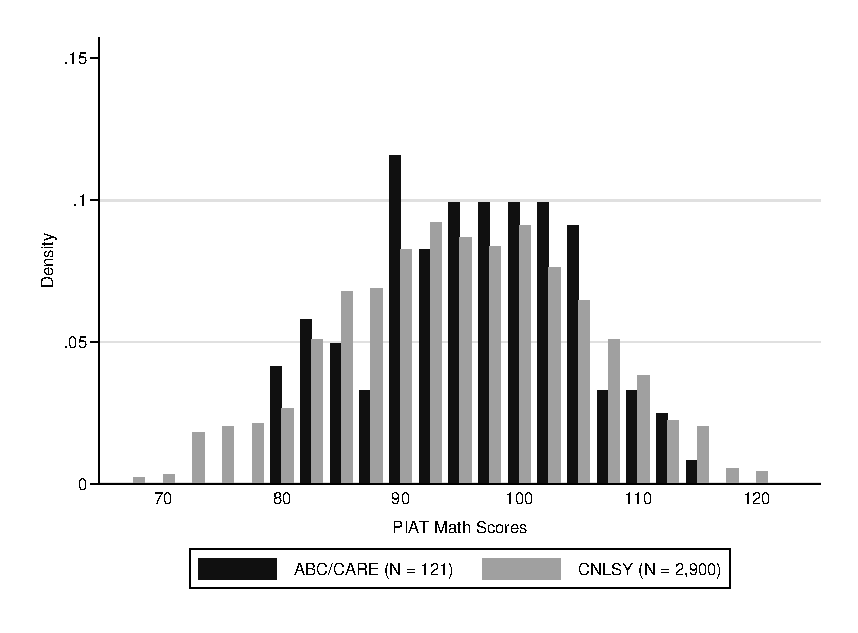
\includegraphics[width=\textwidth]{AppOutput/Methodology/support_math.eps}
	\end{subfigure}
	
	\begin{subfigure}[h]{0.8\textwidth}
	\centering
	\caption{Mother's Years of Education} \label{fig:support_meduc}
	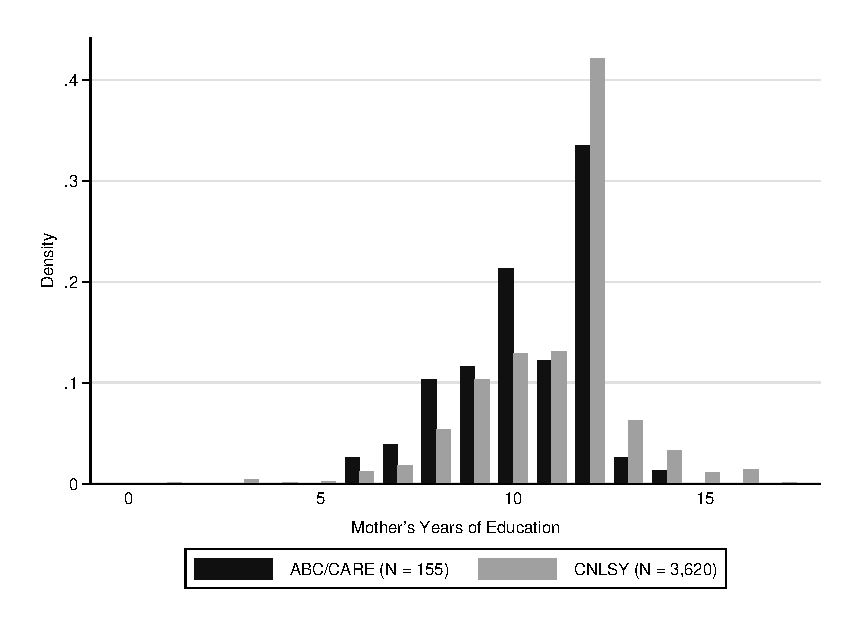
\includegraphics[width=\textwidth]{AppOutput/Methodology/support_momed.eps}
	\end{subfigure}
	
	\floatfoot{
	\footnotesize
	\noindent Note: These graphs display the support of ABC, PSID, NLSY79, and CNLSY
	for variables we use to project future labor income. PIAT math
	scores are averaged over ages 5--7.
	}
\end{figure}

\begin{figure}[H]
		\ContinuedFloat
	\begin{subfigure}[h]{0.8\textwidth}
	\centering
	\caption{Subject's Years of Education} \label{fig:support_educ}
	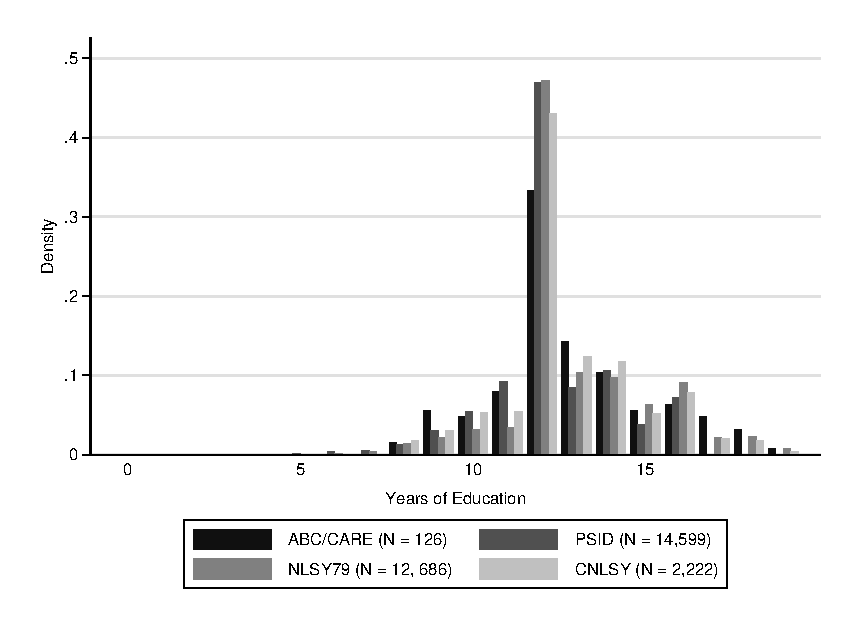
\includegraphics[width=\textwidth]{AppOutput/Methodology/support_educ.eps}
	\end{subfigure}
	
	\begin{subfigure}[h]{0.8\textwidth}
	\centering
	\caption{Income at Age 21} \label{fig:support_inc21}
	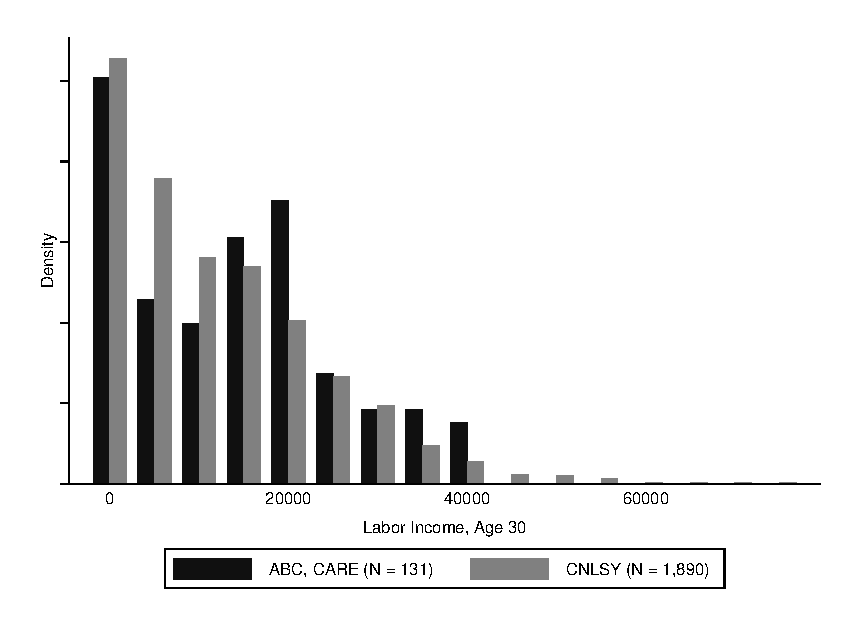
\includegraphics[width=\textwidth]{AppOutput/Methodology/support_inc21.eps}
	\end{subfigure}
	
\end{figure}

\begin{figure}[H]
	\ContinuedFloat
	
	\begin{subfigure}[h]{0.8\textwidth}
	\centering
	\caption{Income at Age 30} \label{fig:support_inc30}
	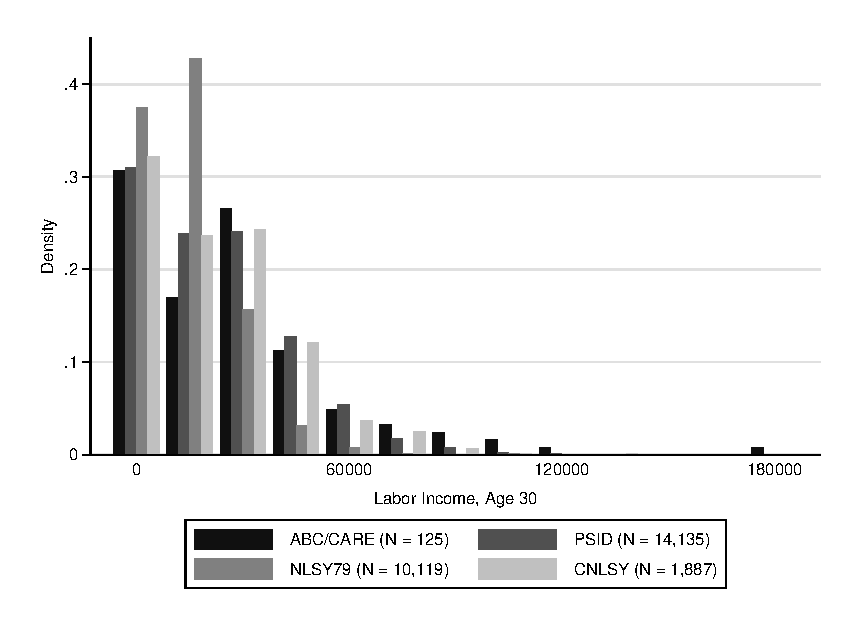
\includegraphics[width=\textwidth]{AppOutput/Methodology/support_inc30.eps}
	\end{subfigure}

	
	\begin{subfigure}[h]{0.8\textwidth}
	\centering
	\caption{Body Mass Index, Age 34} \label{fig:support_bmi}
	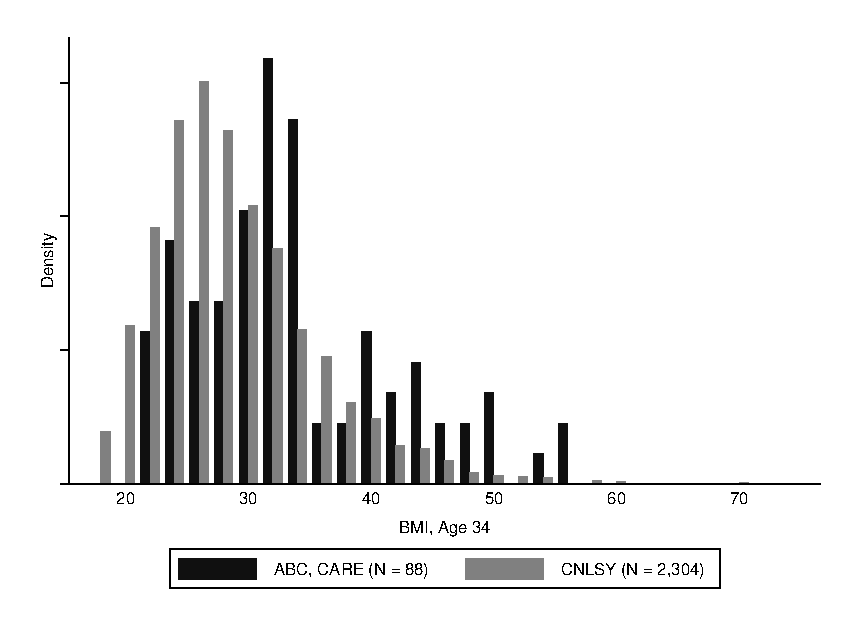
\includegraphics[width=\textwidth]{AppOutput/Methodology/support_bmi.eps}
	\end{subfigure}
	
\end{figure}

\subsubsection{Testing Assumption~\ref{ass:exog}: Exogeneity} \label{app:endogeneity}

\noindent The following framework help us to test both Assumptions~\ref{ass:exog} and \ref{ass:summary}. We provide this framework and test Assumption~\ref{ass:exog} in this section of the appendix, and test Assumption~\ref{ass:summary} in the next section.\\

\noindent Define an outcome vector as

\begin{align}
\bm{Y}_{k,a} &= \bm{X}^d_{k,a} \bm{\gamma} + \bm{\varepsilon}^d_a  &(a) \nonumber
\end{align}

\noindent with an associated measurement system

\begin{align}  \label{eq:sa-msystemmain}
\bm{\varepsilon}_{a}^d &=\bm{\beta}^d \bm{\theta}_{a}^d + \bm{\omega}_{a}^d  &(b) \nonumber \\
\bm{M}_{a}^d &= \bm{\lambda}^d \bm{\theta}_{a}^d + \bm{\upsilon}_a^d,  &(c)
\end{align}


\noindent where $\bm{\theta}^d \independent \bm{\upsilon}_{a}^d, \bm{\omega}_{a}^d$ and $\bm{\upsilon}_{a}^d \independent \bm{\omega}_{a}^d$ for all $a \in \{0, \ldots, A \}, \; d \in \{0,1\}$. We use predictors in these equations. For sake of simplicity, we omit an explicit representation of them here.\\

\noindent When the auxiliary measurement system $\bm{M}_{a}^d $ consists of at least three measures, we are able to identify the vectors of coefficients characterizing this system, $\bm{\lambda}^d, \bm{\beta}^d$, as well as the respective covariance matrices, $\bm{\Sigma}_{\bm{\theta}_{a}^d}, \bm{\Sigma}_{\bm{\upsilon}_{a}^d}, \bm{\Sigma}_{\bm{\omega}_{a}^d}$, and use the method of \citet{Bartlett_1938_Nature} to obtain an estimate of $\bm{\theta}_{a}^d$ \citep{Heckman_Pinto_etal_2013_PerryFactor}. Identifying and estimating the elements in System \eqref{eq:sa-msystemmain} helps two purposes: (i) propose a test of Assumption~\ref{ass:exog}; and (ii) use estimates of $\bm{\theta}_{a}^d$ as control functions when testing Assumption~\ref{ass:summary} in the next appendix, i.e. use these estimates to ``control'' for endogeneity.\\

\noindent We start by providing estimates for the elements in System~\eqref{eq:sa-msystemmain} in the experimental sample. We assume that $\bm{\theta}_{a}^d$ has two dimensions (one representing cognitive skill, $c$, and another representing non-cognitive skill, $n$). We assume dedicated measures for these skills at one time period. Put simply, we have two independent systems, one to measure $\bm{\theta}_{c}^d$ and one to measure $\bm{\theta}_{n}^d$, where $\bm{\theta}_{a}^d: = \left[ \bm{\theta}_{c}^d, \bm{\theta}_{n}^d \right]$. Further, we assume a common measurement system for the treatment and control groups (this is a sensible assumption shown to be true in the Perry data; see \citealp{Heckman_Pinto_etal_2013_PerryFactor}). This assumption implies that $\bm{\lambda}^d, \bm{\beta}^d$, as well as $\bm{\Sigma}_{\bm{\theta}_{a}^d}, \bm{\Sigma}_{\bm{\upsilon}_{a}^d}$ are the same whether $d = 0$ or $d = 1$.\\

\noindent We use a set of IQ measures from ages 2 to 8 to obtain an estimate of $\bm{\theta}_{c}^d$ and a set of measures of somatization, hostility, depression, and mental health all at age 21 to measure to estimate $\bm{\theta}_{n}^d$.\footnote{For definitions and treatment effects on these variables see Appendix~\ref{appendix:results}.} Figure~\ref{figure:factorsm} shows our estimates by treatment status.\\

\begin{figure}[!htbp]
\centering
\caption{Estimates of Cognitive ($\theta_{c}^d$) and Non-cognitive Skills ($\theta_{n}^d$)}\label{figure:factorsm}
\begin{subfigure}[h]{0.5\textwidth}
		\centering
		\caption{Cognitive} \label{fig:c}
		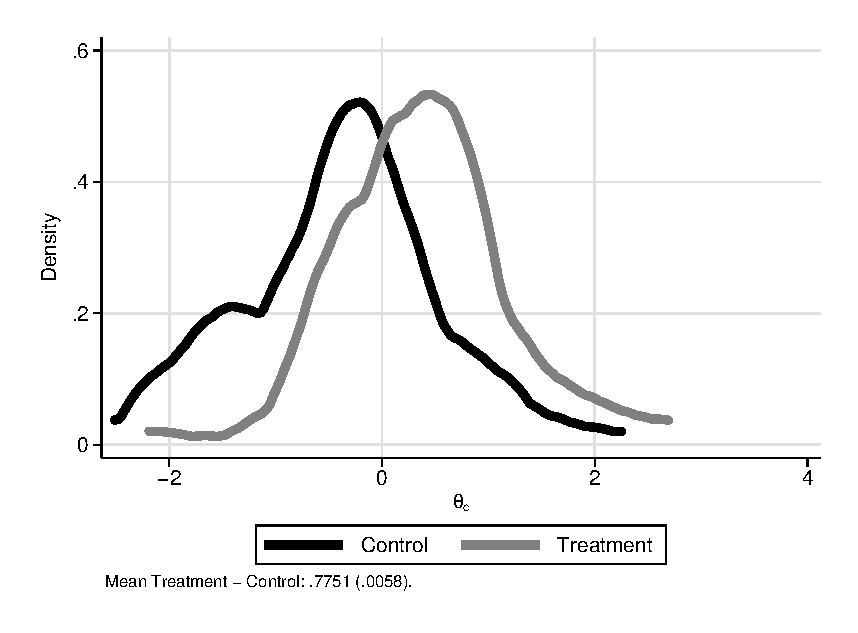
\includegraphics[width=\textwidth]{output/abccare_cfactor.eps}
\end{subfigure}%
\begin{subfigure}[h]{0.5\textwidth}
	\centering
	\caption{Non-cognitive} \label{fig:n}
		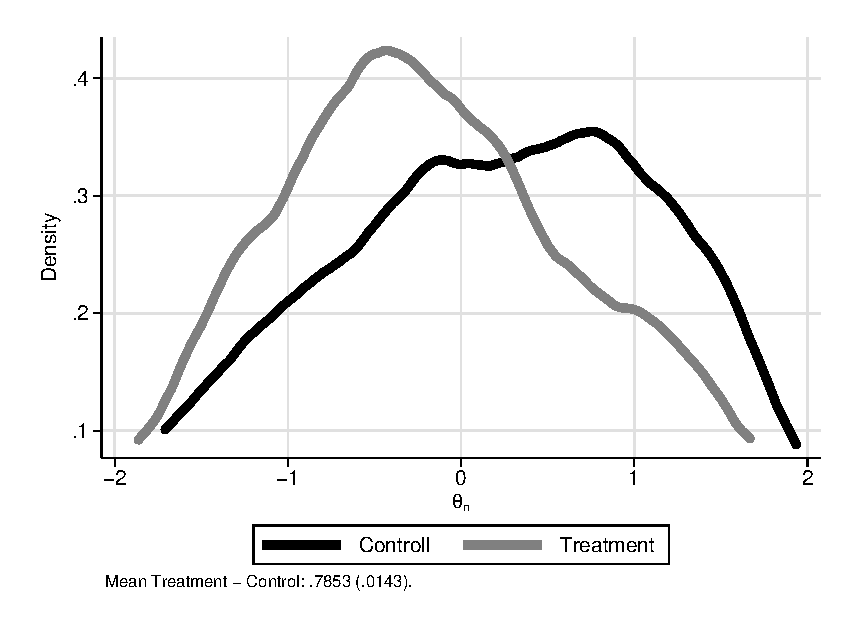
\includegraphics[width=\textwidth]{output/abccare_nfactor.eps}
\end{subfigure}
\footnotesize \justify
Note: Panel (a) displays a factor score estimated based on the measurement system in \eqref{eq:sa-msystemmain} and measures of IQ at ages 2, 3, 4, 5, 7, and 8 (cognitive skill). Panel (b) displays an analogous set of graphs for measures of somatization, hostility, depression, and mental health at age 21 (non-cognitive skill). Both measures of skills are standardized to a mean of $0$ and a standard deviation of $1$. ``Less'' in the factor measuring non-cognitive skills is ``positive'' given the measures we rely on to construct it. The mean difference between treatment and control is displayed below each panel, with standard error in parentheses. Standard errors are based on the empirical bootstrap distribution.
\end{figure}

\noindent We can also estimates $\bm{\theta}_{a}^d$ in the auxiliary sample. For want of data to approximate $\bm{\theta}_{c}, \bm{\theta}_{n}$ in PSID and NLSY79, we use the CNLSY in this appendix. Our measurement system for $\bm{\theta}_{c}$ consists of reading and comprehension PIAT scores as well as by the Peabody Picture Vocabulary Test (PPVT). Our measurement system for $\bm{\theta}_{n}$ is based on six scales of the Behavior Problems Index (e.g., anxiety, dependency, social behavior).\\

\noindent Once these estimates are available, we can test Assumption~\ref{ass:exog} in the experimental and auxiliary samples. The test consists of the following. Let $\bm{\gamma}^E$ be the parameter associated to $\bm{X}^d_{k,a}$ in Equation (a) in System~\eqref{eq:sa-msystemmain} when not accounting for $\bm{\theta}_{a}^d$. Similarly, let $\bm{\gamma}^I$ be the parameter associated with $\bm{X}^d_{k,a}$ in Equation (a) in System~\eqref{eq:sa-msystemmain} when accounting for $\bm{\theta}_{a}^d$. Under the null hypotheses, Assumption~\ref{ass:exog} holds and $\bm{\theta}_{a}^d$ is an irrelevant predictor in Equation (a) in System~\eqref{eq:sa-msystemmain}. This makes the OLS estimate of $\bm{\gamma}^E$ inconsistent. If the null hypotheses are false, $\bm{X}^d_{k,a}$ and $\varepsilon_{a}^d$ are not independent, $\bm{\gamma}^I$ is consistent and $\bm{\gamma}^E$ is not. We test the null hypothesis by asking if the elements in $\bm{\theta}_{a}^d$ are relevant predictors of a set of outcomes at age 30, so that we can perform the tests both the experimental and the auxiliary samples. We contrast specifications with and without including estimates of $\bm{\theta}_{a}^d$, and report the $F$-statistic corresponding to this comparison. This is a version of a Durbin-Wu-Hausman test \citep[see][]{Durbin_1954_RISI,Wu_1973_Econometrica,Hausman_1978_Econometrica}. Tables~\ref{table:endoginc} to \ref{table:trincome} present the results. In most cases, we are not able to reject the null hypothesis that Assumption~\ref{ass:exog} holds.\\


\begin{sidewaystable}[H]
\begin{threeparttable}
\caption{Prediction of Labor Income at Age 30 Accounting for $\bm{B}_k$ and $\bm{\theta}, \bm{X}_{k,a}$, ABC/CARE Control Group}
\label{table:endoginc}
\centering
\footnotesize
\begin{tabular}{lcccccccc} \toprule
 & (1) & (2) & (3) & (4) & (5) & (6) & (7) & (8) \\
 & Estimate & $p$-value & Estimate & $p$-value  & Estimate & $p$-value  & Estimate & $p$-value  \\ \midrule 
Mother's Education &     1,599.57 &         0.17 &       867.41 &         0.34 &      -769.20 &         0.68 &      -580.88 &         0.62 \\  
PIAT (5-7) &            . &            . &            . &            . &        45.98 &         0.41 &       423.44 &         0.20 \\  
Education (30) &            . &            . &            . &            . &     3,415.53 &         0.03 &     4,505.94 &         0.04 \\  
Labor Income (21) &            . &            . &            . &            . &         0.69 &         0.02 &         0.97 &         0.03 \\  
Cognitive &            . &            . &       758.28 &         0.43 &            . &            . &    -8,009.28 &         0.93 \\  
Non Cognitive &            . &            . &      -342.62 &         0.52 &            . &            . &     7,275.49 &         0.09 \\  
Constant &    10,239.82 &         0.28 &    16,530.50 &         0.22 &   -23,140.28 &         0.80 &   -80,679.09 &         0.96 \\  \\ \midrule
R2 &         \multicolumn{2}{c}{0.03} &              \multicolumn{2}{c}{0.07} &             \multicolumn{2}{c}{0.30} &               \multicolumn{2}{c}{0.40}  \\  
Observations &         \multicolumn{2}{c}{66} &          \multicolumn{2}{c}{51} &              \multicolumn{2}{c}{65} &             \multicolumn{2}{c}{63}  \\  \\ \midrule
$F$-stat: exclude Cognitive, Non-Cognitive &              \multicolumn{4}{c}{1.70} &               \multicolumn{4}{c}{4.14}  \\  
$p$-value  &         \multicolumn{4}{c}{0.45} &                   \multicolumn{4}{c}{0.09} \\      \bottomrule \end{tabular}


\begin{tablenotes}
\footnotesize
\item $F$-stat: exclude Cognitive and Non-Cognitive: $F$-statistic contrasting the specifications in columns (1) and (3) and (5) and (7), respectively.\\
\item Note: Prediction of labor income at age 30 based on the variables listed in the row. Empty cells indicate that the variable was not used in the prediction. For each coefficient we provide point estimate and $p$-value for the treatment and control groups and a test for the treatment-control difference. $\hat{\bm{\theta}}_{c}$: factor score estimated based on the measurement system in \eqref{eq:sa-msystemmain} and measures of IQ at ages 2, 3, 4, 5, 7, and 8 (cognitive skill). $\hat{\bm{\theta}}_{n}$: factor score estimated based on the measurement system in \eqref{eq:sa-msystemmain} and measures of somatization, hostility, depression, and a global mental health index at age 21 (non-cognitive skill). Both measures of skills are standardized to a mean of $0$ and a standard deviation of $1$. Inference is based on the empirical bootstrap distribution. If the estimates for the constant terms are in the ten or hundred thousands, we report a figure that has been rounded to the thousands.
\end{tablenotes}
\end{threeparttable}
\end{sidewaystable}

\begin{sidewaystable}[H]
\begin{threeparttable}
\caption{Prediction of Labor Income at Age 30 Accounting for $\bm{B}_k$ and $\bm{\theta}, \bm{X}_{k,a}$, ABC/CARE Treatment Group}
\centering
\footnotesize
\begin{tabular}{lcccccccc} \toprule
 & (1) & (2) & (3) & (4) & (5) & (6) & (7) & (8) \\
 & Estimate & $p$-value & Estimate & $p$-value  & Estimate & $p$-value  & Estimate & $p$-value  \\ \midrule 
Mother's Education &     3,134.16 &         0.23 &     2,600.34 &         0.35 &     2,913.44 &         0.28 &     5,835.67 &         0.22 \\  
PIAT (5-7) &            . &            . &            . &            . &      -263.29 &         0.66 &      -871.06 &         0.76 \\  
Education (30) &            . &            . &            . &            . &    11,600.24 &         0.00 &    13,069.48 &         0.00 \\  
Labor Income (21) &            . &            . &            . &            . &        -0.18 &         0.64 &        -0.62 &         0.75 \\  
Cognitive &            . &            . &     2,766.35 &         0.40 &            . &            . &     4,828.93 &         0.34 \\  
Non Cognitive &            . &            . &     7,600.33 &         0.18 &            . &            . &     6,223.32 &         0.19 \\  
Constant &     3,900.73 &         0.47 &    10,553.93 &         0.42 &  -122,709.85 &         0.91 &  -109,410.81 &         0.76 \\  \\ \midrule
$R^2$ &         \multicolumn{2}{c}{0.02} &          \multicolumn{2}{c}{0.10} &          \multicolumn{2}{c}{0.26} &             \multicolumn{2}{c}{0.33} \\ 
Observations &         \multicolumn{2}{c}{64} &         \multicolumn{2}{c}{49} &                \multicolumn{2}{c}{65} &       \multicolumn{2}{c}{63}  \\   \\ \midrule
$F$-stat: exclude Cognitive, Non-Cognitive &             \multicolumn{4}{c}{3.13} &              \multicolumn{4}{c}{2.14}  \\  
$p$-value &                 \multicolumn{4}{c}{0.27} &                   \multicolumn{4}{c}{0.27}  \\    \bottomrule \end{tabular}


\begin{tablenotes}
\footnotesize
\item $F$-stat: exclude Cognitive and Non-Cognitive: $F$-statistic contrasting the specifications in columns (1) and (3) and (5) and (7), respectively.\\
\item Note: Prediction of labor income at age 30 based on the variables listed in the row. Empty cells indicate that the variable was not used in the prediction. For each coefficient we provide point estimate and $p$-value for the treatment and control groups and a test for the treatment-control difference. $\hat{\bm{\theta}}_{c}$: factor score estimated based on the measurement system in \eqref{eq:sa-msystemmain} and measures of IQ at ages 2, 3, 4, 5, 7, and 8 (cognitive skill). $\hat{\bm{\theta}}_{n}$: factor score estimated based on the measurement system in \eqref{eq:sa-msystemmain} and measures of somatization, hostility, depression, and a global mental health index at age 21 (non-cognitive skill). Both measures of skills are standardized to a mean of $0$ and a standard deviation of $1$. Inference is based on the empirical bootstrap distribution. If the estimates for the constant terms are in the ten or hundred thousands, we report a figure that has been rounded to the thousands.
\end{tablenotes}
\end{threeparttable}
\end{sidewaystable}

\begin{sidewaystable}[H]
\begin{threeparttable}
\caption{Prediction of Labor Income at Age 30 Accounting for $\bm{B}_k$ and $\bm{\theta}, \bm{X}_{k,a}$, ABC/CARE Control and Treatment Groups}
\centering
\footnotesize
\begin{tabular}{lcccccccc} \toprule
 & (1) & (2) & (3) & (4) & (5) & (6) & (7) & (8) \\
 & Estimate & $p$-value & Estimate & $p$-value  & Estimate & $p$-value  & Estimate & $p$-value  \\ \midrule 
Mother's Education &     2,668.48 &         0.12 &     2,200.35 &         0.25 &       794.11 &         0.36 &     1,724.88 &         0.31 \\  
PIAT (5-7) &            . &            . &            . &            . &      -126.19 &         0.67 &      -400.57 &         0.72 \\  
Education (30) &            . &            . &            . &            . &     8,601.33 &         0.00 &     9,706.02 &         0.00 \\  
Labor Income (21) &            . &            . &            . &            . &         0.14 &         0.37 &         0.21 &         0.37 \\  
Cognitive &            . &            . &     4,260.39 &         0.16 &            . &            . &     1,427.18 &         0.44 \\  
Non Cognitive &            . &            . &     2,899.66 &         0.25 &            . &            . &     7,557.01 &         0.05 \\  
Constant &     4,443.37 &         0.41 &     9,166.30 &         0.38 &   -78,053.28 &         0.95 &   -75,621.84 &         0.87 \\  \\ \midrule
$R^2$ &         \multicolumn{2}{c}{0.02} &          \multicolumn{2}{c}{0.04} &             \multicolumn{2}{c}{0.20} &                 \multicolumn{2}{c}{0.25}  \\  
Observations &        \multicolumn{2}{c}{132} &        \multicolumn{2}{c}{100} &     \multicolumn{2}{c}{130} &         \multicolumn{2}{c}{133}  \\  \\ \midrule
$F$-stat: exclude Cognitive, Non-Cognitive  &             \multicolumn{4}{c}{2.07} &               \multicolumn{4}{c}{2.92}  \\  
$p$-value &                \multicolumn{4}{c}{0.31} &               \multicolumn{4}{c}{0.19}   \\  \bottomrule \end{tabular}
\begin{tablenotes}
\footnotesize
\item $F$-stat: exclude Cognitive and Non-Cognitive: $F$-statistic contrasting the specifications in columns (1) and (3) and (5) and (7), respectively.\\
\item Note: Prediction of labor income at age 30 based on the variables listed in the row. Empty cells indicate that the variable was not used in the prediction. For each coefficient we provide point estimate and $p$-value for the treatment and control groups and a test for the treatment-control difference. $\hat{\bm{\theta}}_{c}$: factor score estimated based on the measurement system in \eqref{eq:sa-msystemmain} and measures of IQ at ages 2, 3, 4, 5, 7, and 8 (cognitive skill). $\hat{\bm{\theta}}_{n}$: factor score estimated based on the measurement system in \eqref{eq:sa-msystemmain} and measures of somatization, hostility, depression, and a global mental health index at age 21 (non-cognitive skill). Both measures of skills are standardized to a mean of $0$ and a standard deviation of $1$. Inference is based on the empirical bootstrap distribution. If the estimates for the constant terms are in the ten or hundred thousands, we report a figure that has been rounded to the thousands.
\end{tablenotes}
\end{threeparttable}
\end{sidewaystable}

\begin{sidewaystable}[H]
\begin{threeparttable}
\caption{Prediction of Labor Income at Age 30 Accounting for $\bm{B}_k$ and $\bm{\theta}, \bm{X}_{k,a}$, CNLSY}
\centering
\footnotesize
\begin{tabular}{lcccccccc} \toprule
 & (1) & (2) & (3) & (4) & (5) & (6) & (7) & (8) \\
 & Estimate & $p$-value & Estimate & $p$-value  & Estimate & $p$-value  & Estimate & $p$-value  \\ \midrule 
Mother's Education &     2,317.52 &         0.00 &     2,262.79 &         0.00 &       316.78 &         0.23 &       379.54 &         0.32 \\  
PIAT (5-7) &            . &            . &            . &            . &       263.98 &         0.00 &       471.53 &         0.00 \\  
Education (30) &            . &            . &            . &            . &     3,647.75 &         0.00 &     4,351.32 &         0.00 \\  
Labor Income (21) &            . &            . &            . &            . &         0.68 &         0.00 &         0.79 &         0.00 \\  
Cognitive &            . &            . &     2,680.61 &         0.13 &            . &            . &    -4,541.18 &         0.95 \\  
Non Cognitive &            . &            . &    -3,584.83 &         0.99 &            . &            . &    -1,352.32 &         0.79 \\  
Constant &     2,523.10 &         0.25 &     3,699.61 &         0.37 &   -56,008.30 &         1.00 &   -86,767.50 &         1.00 \\ \\ \midrule
$R^2$ &         \multicolumn{2}{c}{0.03} &              \multicolumn{2}{c}{0.06} &               \multicolumn{2}{c}{0.21} &                \multicolumn{2}{c}{0.34}  \\  
Observations &       \multicolumn{2}{c}{1,885} &            \multicolumn{2}{c}{370} &           \multicolumn{2}{c}{1,885} &          \multicolumn{2}{c}{1,883}   \\  \\ \midrule
$F$-stat: exclude Cognitive, Non-Cognitive &                      \multicolumn{4}{c}{5.90} &                      \multicolumn{4}{c}{3.11}   \\  
$p$-value &             \multicolumn{4}{c}{0.05} &                  \multicolumn{4}{c}{0.18}  \\    \bottomrule \end{tabular}

\begin{tablenotes}
\footnotesize
\item $F$-stat: exclude Cognitive and Non-Cognitive: $F$-statistic contrasting the specifications in columns (1) and (3) and (5) and (7), respectively.\\
\item Note: Prediction of labor income at age 30 based on the variables listed in the row. Empty cells indicate that the variable was not used in the prediction. For each coefficient we provide point estimate and $p$-value for the treatment and control groups and a test for the treatment-control difference. $\hat{\bm{\theta}}_{c}$: factor score estimated based on the measurement system in \eqref{eq:sa-msystemmain} and measures of reading and comprehension of the PIAT, as weel as the Peabody Picture Vocabulary Test (PPVT) (cognitive skill). $\hat{\bm{\theta}}_{n}$: factor score estimated based on the measurement system in \eqref{eq:sa-msystemmain} and six scales of the Behavior Problems Index (e.g., anxiety, dependency, social behavior) (non-cognitive skill). Both measures of skills are standardized to a mean of $0$ and a standard deviation of $1$. Inference is based on the empirical bootstrap distribution. If the estimates for the constant terms are in the ten or hundred thousands, we report a figure that has been rounded to the thousands.
\end{tablenotes}
\end{threeparttable}
\end{sidewaystable}

\begin{sidewaystable}[H]
\begin{threeparttable}
\caption{Prediction of Transfer Income at Age 30 Accounting for $\bm{B}_k$ and $\bm{\theta}, \bm{X}_{k,a}$, ABC/CARE Control Group}
\label{table:endoginc}
\centering
\footnotesize
\begin{tabular}{lcccccccc} \toprule
 & (1) & (2) & (3) & (4) & (5) & (6) & (7) & (8) \\
 & Estimate & $p$-value & Estimate & $p$-value  & Estimate & $p$-value  & Estimate & $p$-value  \\ \midrule 
Mother's Education &      -413.76 &         0.78 &      -406.14 &         0.69 &        48.75 &         0.49 &        51.97 &         0.47 \\  
PIAT (5-7) &            . &            . &            . &            . &        27.10 &         0.29 &      -101.93 &         0.77 \\  
Education (30) &            . &            . &            . &            . &      -684.75 &         0.99 &      -693.44 &         0.91 \\  
Labor Income (21) &            . &            . &            . &            . &        -0.14 &         0.99 &        -0.15 &         0.93 \\  
Cognitive &            . &            . &      -348.53 &         0.69 &            . &            . &     1,696.96 &         0.13 \\  
Non Cognitive &            . &            . &     1,622.92 &         0.05 &            . &            . &       887.17 &         0.19 \\  \\ \midrule 
$R^2$ &          \multicolumn{2}{c}{0.04} &             \multicolumn{2}{c}{0.15} &            \multicolumn{2}{c}{0.21} &              \multicolumn{2}{c}{0.27}   \\  
Observations &         \multicolumn{2}{c}{68} &                 \multicolumn{2}{c}{52} &               \multicolumn{2}{c}{70}  &                \multicolumn{2}{c}{70}   \\  \\ \midrule
$F$-stat: exclude Cognitive, Non-Cognitive  &                 \multicolumn{4}{c}{2.36} &              \multicolumn{4}{c}{3.50}  \\  
$p$-value &                \multicolumn{4}{c}{0.30} &               \multicolumn{4}{c}{0.30}  \\      \bottomrule \end{tabular}
\begin{tablenotes}
\footnotesize
\item $F$-stat: exclude Cognitive and Non-Cognitive: $F$-statistic contrasting the specifications in columns (1) and (3) and (5) and (7), respectively.\\
\item Note: Prediction of transfer income at age 30 based on the variables listed in the row. Empty cells indicate that the variable was not used in the prediction. For each coefficient we provide point estimate and $p$-value for the treatment and control groups and a test for the treatment-control difference. $\hat{\bm{\theta}}_{c}$: factor score estimated based on the measurement system in \eqref{eq:sa-msystemmain} and measures of IQ at ages 2, 3, 4, 5, 7, and 8 (cognitive skill). $\hat{\bm{\theta}}_{n}$: factor score estimated based on the measurement system in \eqref{eq:sa-msystemmain} and measures of somatization, hostility, depression, and a global mental health index at age 21 (non-cognitive skill). Both measures of skills are standardized to a mean of $0$ and a standard deviation of $1$. Inference is based on the empirical bootstrap distribution. If the estimates for the constant terms are in the ten or hundred thousands, we report a figure that has been rounded to the thousands.
\end{tablenotes}
\end{threeparttable}
\end{sidewaystable}

\begin{sidewaystable}[H]
\begin{threeparttable}
\caption{Prediction of Transfer Income at Age 30 Accounting for $\bm{B}_k$ and $\bm{\theta}, \bm{X}_{k,a}$, ABC/CARE Treatment Group}
\centering
\footnotesize
\begin{tabular}{lcccccccc} \toprule
 & (1) & (2) & (3) & (4) & (5) & (6) & (7) & (8) \\
 & Estimate & $p$-value & Estimate & $p$-value  & Estimate & $p$-value  & Estimate & $p$-value  \\ \midrule 
Mother'sEducation &      -212.39 &         0.75 &      -336.44 &         0.81 &      -199.39 &         0.74 &      -302.60 &         0.79 \\  
PIAT(5-7) &            . &            . &            . &            . &       -46.36 &         0.86 &       -22.41 &         0.65 \\  
Education(30) &            . &            . &            . &            . &       -35.62 &         0.56 &       -72.66 &         0.59 \\  
LaborIncome(21) &            . &            . &            . &            . &        -0.05 &         0.94 &        -0.05 &         0.90 \\  
Cognitive &            . &            . &      -421.59 &         0.75 &            . &            . &      -273.48 &         0.62 \\  
Non Cognitive &            . &            . &      -825.26 &         0.95 &            . &            . &      -987.11 &         0.98 \\  
Constant &     3,348.22 &         0.16 &     4,937.75 &         0.14 &     9,041.98 &         0.09 &     8,432.47 &         0.18 \\  \\ \midrule
$R^2$  &          \multicolumn{2}{c}{0.03} &            \multicolumn{2}{c}{0.15} &                  \multicolumn{2}{c}{0.13} &               \multicolumn{2}{c}{0.25}  \\  
Observations &        \multicolumn{2}{c}{63} &               \multicolumn{2}{c}{49}  &             \multicolumn{2}{c}{65}  &         \multicolumn{2}{c}{63}  \\   \\ \midrule
$F$-stat: exclude Cognitive, Non-Cognitive &                    \multicolumn{4}{c}{3.08} &                   \multicolumn{4}{c}{2.79}  \\  
$p$-value &              \multicolumn{4}{c}{0.20} &                    \multicolumn{4}{c}{0.18}  \\      \bottomrule \end{tabular}
\begin{tablenotes}
\footnotesize
\item $F$-stat: exclude Cognitive and Non-Cognitive: $F$-statistic contrasting the specifications in columns (1) and (3) and (5) and (7), respectively.\\
\item Note: Prediction of transfer income at age 30 based on the variables listed in the row. Empty cells indicate that the variable was not used in the prediction. For each coefficient we provide point estimate and $p$-value for the treatment and control groups and a test for the treatment-control difference. $\hat{\bm{\theta}}_{c}$: factor score estimated based on the measurement system in \eqref{eq:sa-msystemmain} and measures of IQ at ages 2, 3, 4, 5, 7, and 8 (cognitive skill). $\hat{\bm{\theta}}_{n}$: factor score estimated based on the measurement system in \eqref{eq:sa-msystemmain} and measures of somatization, hostility, depression, and a global mental health index at age 21 (non-cognitive skill). Both measures of skills are standardized to a mean of $0$ and a standard deviation of $1$. Inference is based on the empirical bootstrap distribution. If the estimates for the constant terms are in the ten or hundred thousands, we report a figure that has been rounded to the thousands.
\end{tablenotes}
\end{threeparttable}
\end{sidewaystable}

\begin{sidewaystable}[H]
\begin{threeparttable}
\caption{Prediction of Transfer Income at Age 30 Accounting for $\bm{B}_k$ and $\bm{\theta}, \bm{X}_{k,a}$, ABC/CARE Control and Treatment Groups}
\centering
\footnotesize
\begin{tabular}{lcccccccc} \toprule
 & (1) & (2) & (3) & (4) & (5) & (6) & (7) & (8) \\
 & Estimate & $p$-value & Estimate & $p$-value  & Estimate & $p$-value  & Estimate & $p$-value  \\ \midrule 
Mother's Education &      -299.72 &         0.81 &      -411.12 &         0.85 &      -135.23 &         0.62 &      -211.76 &         0.68 \\  
PIAT (5-7) &            . &            . &            . &            . &       -34.90 &         0.81 &       -66.99 &         0.80 \\  
Education (30) &            . &            . &            . &            . &      -430.88 &         0.96 &      -453.82 &         0.96 \\  
Labor Income (21) &            . &            . &            . &            . &        -0.09 &         1.00 &        -0.08 &         0.96 \\  
Cognitive &            . &            . &      -753.98 &         0.93 &            . &            . &       153.54 &         0.42 \\  
Non Cognitive &            . &            . &       631.74 &         0.17 &            . &            . &       264.49 &         0.34 \\  
Constant &     5,135.83 &         0.06 &     6,460.15 &         0.07 &    13,548.68 &         0.03 &    17,791.02 &         0.05 \\   \\ \midrule
$R^2$ &         \multicolumn{2}{c}{0.02} &         \multicolumn{2}{c}{0.10} &               \multicolumn{2}{c}{0.15} &            \multicolumn{2}{c}{0.18}  \\  
Observations &       \multicolumn{2}{c}{133} &           \multicolumn{2}{c}{101} &         \multicolumn{2}{c}{135} &            \multicolumn{2}{c}{133}  \\  \\ \midrule
$F$-stat: exclude Cognitive, Non-Cognitive &              \multicolumn{4}{c}{1.44} &             \multicolumn{4}{c}{1.10}  \\  
$p$-value &            \multicolumn{4}{c}{0.44} &               \multicolumn{4}{c}{0.44}  \\   \bottomrule \end{tabular}


\begin{tablenotes}
\footnotesize
\item $F$-stat: exclude Cognitive and Non-Cognitive: $F$-statistic contrasting the specifications in columns (1) and (3) and (5) and (7), respectively.\\
\item Note: Prediction of transfer income at age 30 based on the variables listed in the row. Empty cells indicate that the variable was not used in the prediction. For each coefficient we provide point estimate and $p$-value for the treatment and control groups and a test for the treatment-control difference. $\hat{\bm{\theta}}_{c}$: factor score estimated based on the measurement system in \eqref{eq:sa-msystemmain} and measures of IQ at ages 2, 3, 4, 5, 7, and 8 (cognitive skill). $\hat{\bm{\theta}}_{n}$: factor score estimated based on the measurement system in \eqref{eq:sa-msystemmain} and measures of somatization, hostility, depression, and a global mental health index at age 21 (non-cognitive skill). Both measures of skills are standardized to a mean of $0$ and a standard deviation of $1$. Inference is based on the empirical bootstrap distribution. If the estimates for the constant terms are in the ten or hundred thousands, we report a figure that has been rounded to the thousands.
\end{tablenotes}
\end{threeparttable}
\end{sidewaystable}

\begin{sidewaystable}[H]
\begin{threeparttable}
\caption{Prediction of Transfer Income at Age 30 Accounting for $\bm{B}_k$ and $\bm{\theta}, \bm{X}_{k,a}$, CNLSY} \label{table:trincome}
\centering
\footnotesize
\begin{tabular}{lcccccccc} \toprule
 & (1) & (2) & (3) & (4) & (5) & (6) & (7) & (8) \\
 & Estimate & $p$-value & Estimate & $p$-value  & Estimate & $p$-value  & Estimate & $p$-value  \\ \midrule 
Mother'sEducation &      -457.46 &         0.56 &     8,259.13 &         0.04 &       985.13 &         0.41 &     9,344.69 &         0.02 \\  
PIAT(5-7) &            . &            . &            . &            . &      -273.46 &         0.64 &      -506.25 &         0.70 \\  
Education(30) &            . &            . &            . &            . &    -7,235.35 &         0.96 &    -5,622.52 &         0.84 \\  
LaborIncome(21) &            . &            . &            . &            . &         0.17 &         0.40 &        -0.96 &         0.98 \\  
Cognitive &            . &            . &    -8,525.66 &         0.83 &            . &            . &      -473.24 &         0.52 \\  
NonCognitive &            . &            . &    18,373.65 &         0.03 &            . &            . &     6,585.57 &         0.22 \\  
Constant &    34,777.07 &         0.14 &   -58,507.25 &         0.91 &   137,947.14 &         0.14 &    57,813.64 &         0.35 \\  \\ \midrule
$R^2$ &         \multicolumn{2}{c}{0.00} &               \multicolumn{2}{c}{0.02} &                \multicolumn{2}{c}{0.01} &             \multicolumn{2}{c}{0.05}   \\  
Observations &       \multicolumn{2}{c}{1,145} &              \multicolumn{2}{c}{244}  &       \multicolumn{2}{c}{1,145} &      \multicolumn{2}{c}{1,148}   \\  \\ \midrule
$F$-stat: exclude Cognitive, Non-Cognitive &                \multicolumn{4}{c}{1.85} &                 \multicolumn{4}{c}{1.04}   \\  
$p$-value  &                \multicolumn{4}{c}{0.34} &                \multicolumn{4}{c}{0.34}    \\  \bottomrule \end{tabular}


\begin{tablenotes}
\footnotesize
\item $F$-stat: exclude Cognitive and Non-Cognitive: $F$-statistic contrasting the specifications in columns (1) and (3) and (5) and (7), respectively.\\
\item Note: Prediction of transfer income at age 30 based on the variables listed in the row. Empty cells indicate that the variable was not used in the prediction. For each coefficient we provide point estimate and $p$-value for the treatment and control groups and a test for the treatment-control difference.$\hat{\bm{\theta}}_{c}$: factor score estimated based on the measurement system in \eqref{eq:sa-msystemmain} and measures of reading and comprehension of the PIAT, as weel as the Peabody Picture Vocabulary Test (PPVT) (cognitive skill). $\hat{\bm{\theta}}_{n}$: factor score estimated based on the measurement system in \eqref{eq:sa-msystemmain} and six scales of the Behavior Problems Index (e.g., anxiety, dependency, social behavior) (non-cognitive skill).  Both measures of skills are standardized to a mean of $0$ and a standard deviation of $1$. Inference is based on the empirical bootstrap distribution. If the estimates for the constant terms are in the ten or hundred thousands, we report a figure that has been rounded to the thousands.
\end{tablenotes}
\end{threeparttable}
\end{sidewaystable}

\subsubsection{Testing Assumption~\ref{ass:summary}: Structural Invariance} \label{app:invariance}

In this appendix, we use the framework in Appendix~\ref{app:endogeneity} to tests Assumption~\ref{ass:summary}. The tests are under the null hypothesis that Assumption~\ref{ass:exog} holds. In the main text we show that Assumption~\ref{ass:summary}, together with Assumption~\ref{ass:exog}, implies:

\begin{equation}\label{eq:invariancetestapp}
\mathbb{E} \left[ Y_{k,j,a}^d | \bm{X}_{k,a}^d  = \bm{x}, \bm{B}_k = \bm{b}, D = d \right] = \mathbb{E} \left[ Y_{k,j,a} | \bm{X}^d_{k,a}  = \bm{x}, \bm{B}_k = \bm{b} \right],
\end{equation}
for $a \in \{1,\dots,A\}$, $k \in \{e,n\}$, and $d \in \{0,1\}$.\\

\noindent A direct test of this hypothesis is to use the experimental sample and ask if once we account for a set of the variables in $\bm{X}_{k,a}$, $R$ (randomization to treatment assignment in ABC/CARE, which, as discussed in text, is equivalent to $D$) predicts the outcome of interest, conditional on $\bm{B}_k$. This tests if this specific set of $\bm{X}_{k,a}$ suffices to summarize the treatment generated by $R$. Under the null hypothesis, the coefficient associated to $R$ when predicting based on $\bm{B}_k$ and $\bm{X}_{k,a}$ is zero. We test this using the following predictors. Average Mathematics PIAT scores at ages 5 to 7, education at age 30, and labor income at age 21. That is, children who are offered treatment attend it. For a set of outcomes of interest, even beyond those that we predict, once we condition on $\bm{B}_k, \bm{X}_{k,a}, \bm{\theta}$, the coefficient associated with $R$ is not significant. We test this with and without accounting for endogeneity, as explained in Appendix~\ref{app:endogeneity}.\\

\begin{sidewaystable}[H]
\begin{threeparttable}
\caption{Prediction of High School Graduation at Age 30 Accounting for $R, \bm{B}_k, \bm{\theta},$ and $\bm{X}_{k,a}$ Pooled Sample, ABC/CARE}
\label{table:end2}
\centering
\scriptsize
\begin{tabular}{lcccccccc} \toprule
 & (1) & (2) & (3) & (4) & (5) & (6) & (7) & (8) \\ 
 & Estimate  & $p$-value  & Estimate  & $p$-value  & Estimate  & $p$-value  & Estimate  & $p$-value  \\  \midrule
$R$ &     0.130 &     0.040 &     0.106 &     0.170 &     0.019 &     0.415 &     0.019 &     0.425 \\  
Mother's Education &     0.093 &     0.000 &     0.081 &     0.000 &     0.051 &     0.000 &     0.043 &     0.050 \\  
PIAT (5-7) &         . &         . &         . &         . &    -0.005 &     0.910 &    -0.004 &     0.765 \\  
Education (30) &         . &         . &         . &         . &     0.119 &     0.000 &     0.124 &     0.000 \\  
Labor Income (21) &         . &         . &         . &         . &     0.000 &     0.005 &     0.000 &     0.010 \\  
Cognitive &         . &         . &     0.020 &     0.360 &         . &         . &    -0.038 &     0.740 \\  
Non Cognitive &         . &         . &    -0.027 &     0.720 &         . &         . &     0.011 &     0.395 \\  
Constant &    -0.410 &     0.985 &    -0.283 &     0.865 &    -1.082 &     1.000 &    -1.148 &     0.985 \\  \\ \midrule
$F$-stat &    \multicolumn{2}{c}{14.497} &          \multicolumn{2}{c}{5.819} &         \multicolumn{2}{c}{40.509} &           \multicolumn{2}{c}{25.147} \\  
$R^2$ &     \multicolumn{2}{c}{0.151} &          \multicolumn{2}{c}{0.143} &              \multicolumn{2}{c}{0.440} &          \multicolumn{2}{c}{0.434} \\  
Observations &   \multicolumn{2}{c}{134} &           \multicolumn{2}{c}{102} &          \multicolumn{2}{c}{135} &         \multicolumn{2}{c}{133} \\  \bottomrule \end{tabular}

\begin{tablenotes}
\footnotesize
\item Note: Prediction of high school graduation at age 30 based on the variables listed in the row. Empty cells indicate that the variable was not used in the prediction. For each coefficient we provide point estimate and $p$-value. $\hat{\bm{\theta}}_{c}$: factor score estimated based on the measurement system in \eqref{eq:sa-msystemmain} and PIAT sections that we do not use to predict (reading and comprehension) as well as by the Peabody Picture Vocabulary Test (PPVT) (cognitive skill). $\hat{\bm{\theta}}_{n}$: factor score estimated based on the measurement system in \eqref{eq:sa-msystemmain} and on six scales of the Behavior Problems Index (e.g., anxiety, dependency, social behavior). Inference is based on the empirical bootstrap distribution. If the estimates for the constant terms are in the ten or hundred thousands, we report a figure that has been rounded to the thousands.
\end{tablenotes}
\end{threeparttable}
\end{sidewaystable}

\begin{sidewaystable}[H]
\begin{threeparttable}
\caption{Prediction of High School Graduation at Age 30 Accounting for $R, \bm{B}_k, \bm{\theta},$ and $\bm{X}_{k,a}$ Female Sample, ABC/CARE}
\label{table:end2}
\centering
\scriptsize
\begin{tabular}{lcccccccc} \toprule
 & (1) & (2) & (3) & (4) & (5) & (6) & (7) & (8) \\ 
 & Estimate  & $p$-value  & Estimate  & $p$-value  & Estimate  & $p$-value  & Estimate  & $p$-value  \\  \midrule
$R$ &     0.196 &     0.010 &     0.091 &     0.250 &     0.031 &     0.385 &     0.037 &     0.425 \\  
Mother's Education &     0.077 &     0.000 &     0.062 &     0.050 &     0.036 &     0.055 &     0.023 &     0.170 \\  
PIAT (5-7) &         . &         . &         . &         . &    -0.008 &     0.860 &    -0.004 &     0.655 \\  
Education (30) &         . &         . &         . &         . &     0.093 &     0.000 &     0.102 &     0.005 \\  
Labor Income (21) &         . &         . &         . &         . &     0.000 &     0.000 &     0.000 &     0.000 \\  
Cognitive &         . &         . &     0.051 &     0.285 &         . &         . &    -0.073 &     0.775 \\  
Non Cognitive &         . &         . &    -0.076 &     0.895 &         . &         . &     0.051 &     0.200 \\  
Constant &    -0.266 &     0.800 &    -0.065 &     0.540 &    -0.444 &     0.790 &    -0.872 &     0.870 \\  \\ \midrule
$F$-stat &    \multicolumn{2}{c}{10.180} &     \multicolumn{2}{c}{5.545} &          \multicolumn{2}{c}{35.887} &          \multicolumn{2}{c}{31.753} \\  
$R^2$ &     \multicolumn{2}{c}{0.172} &         \multicolumn{2}{c}{0.197} &         \multicolumn{2}{c}{0.556} &           \multicolumn{2}{c}{0.612}  \\  
Observations &    \multicolumn{2}{c}{68} &         \multicolumn{2}{c}{53} &          \multicolumn{2}{c}{70} &          \multicolumn{2}{c}{70} \\  \bottomrule 
\end{tabular}


\begin{tablenotes}
\footnotesize
\item Note: Prediction of high school graduation at age 30 based on the variables listed in the row. Empty cells indicate that the variable was not used in the prediction. For each coefficient we provide point estimate and $p$-value. $\hat{\bm{\theta}}_{c}$: factor score estimated based on the measurement system in \eqref{eq:sa-msystemmain} and PIAT sections that we do not use to predict (reading and comprehension) as well as by the Peabody Picture Vocabulary Test (PPVT) (cognitive skill). $\hat{\bm{\theta}}_{n}$: factor score estimated based on the measurement system in \eqref{eq:sa-msystemmain} and on six scales of the Behavior Problems Index (e.g., anxiety, dependency, social behavior). Inference is based on the empirical bootstrap distribution. If the estimates for the constant terms are in the ten or hundred thousands, we report a figure that has been rounded to the thousands.
\end{tablenotes}
\end{threeparttable}
\end{sidewaystable}

\begin{sidewaystable}[H]
\begin{threeparttable}
\caption{Prediction of High School Graduation at Age 30 Accounting for $R, \bm{B}_k, \bm{\theta},$ and $\bm{X}_{k,a}$ Male Sample, ABC/CARE}
\label{table:end2}
\centering
\scriptsize
\begin{tabular}{lcccccccc} \toprule
 & (1) & (2) & (3) & (4) & (5) & (6) & (7) & (8) \\ 
 & Estimate  & $p$-value  & Estimate  & $p$-value  & Estimate  & $p$-value  & Estimate  & $p$-value  \\  \midrule
$R$ &     0.084 &     0.220 &     0.146 &     0.140 &     0.088 &     0.190 &     0.067 &     0.305 \\  
Mother's Education &     0.116 &     0.000 &     0.131 &     0.000 &     0.057 &     0.045 &     0.072 &     0.095 \\  
PIAT (5-7) &         . &         . &         . &         . &     0.000 &     0.470 &    -0.000 &     0.500 \\  
Education (30) &         . &         . &         . &         . &     0.152 &     0.000 &     0.156 &     0.000 \\  
Labor Income (21) &         . &         . &         . &         . &     0.000 &     0.170 &     0.000 &     0.440 \\  
Cognitive &         . &         . &    -0.023 &     0.645 &         . &         . &    -0.009 &     0.525 \\  
Non Cognitive &         . &         . &     0.051 &     0.195 &         . &         . &     0.004 &     0.475 \\  
Constant &    -0.636 &     0.970 &    -0.824 &     0.950 &    -2.092 &     1.000 &    -2.227 &     0.955 \\  \\ \hline
$F$-stat &    \multicolumn{2}{c}{11.144} &          \multicolumn{2}{c}{6.555} &           \multicolumn{2}{c}{17.009} &    \multicolumn{2}{c}{10.294}  \\  
$R^2$ &     \multicolumn{2}{c}{0.190} &            \multicolumn{2}{c}{0.215} &           \multicolumn{2}{c}{0.467} &     \multicolumn{2}{c}{0.460}  \\  
Observations &    \multicolumn{2}{c}{67} &           \multicolumn{2}{c}{49} &           \multicolumn{2}{c}{65} &   \multicolumn{2}{c}{70} \\  
\bottomrule \end{tabular}

\begin{tablenotes}
\footnotesize
\item Note: Prediction of high school graduation at age 30 based on the variables listed in the row. Empty cells indicate that the variable was not used in the prediction. For each coefficient we provide point estimate and $p$-value. $\hat{\bm{\theta}}_{c}$: factor score estimated based on the measurement system in \eqref{eq:sa-msystemmain} and PIAT sections that we do not use to predict (reading and comprehension) as well as by the Peabody Picture Vocabulary Test (PPVT) (cognitive skill). $\hat{\bm{\theta}}_{n}$: factor score estimated based on the measurement system in \eqref{eq:sa-msystemmain} and on six scales of the Behavior Problems Index (e.g., anxiety, dependency, social behavior). Inference is based on the empirical bootstrap distribution. If the estimates for the constant terms are in the ten or hundred thousands, we report a figure that has been rounded to the thousands.
\end{tablenotes}
\end{threeparttable}
\end{sidewaystable}


\begin{sidewaystable}[H]
\begin{threeparttable}
\caption{Prediction of Employment at Age 30 Accounting for $R, \bm{B}_k, \bm{\theta},$ and $\bm{X}_{k,a}$ Pooled Sample, ABC/CARE}
\label{table:end2}
\centering
\scriptsize
\begin{tabular}{lcccccccc} \toprule
 & (1) & (2) & (3) & (4) & (5) & (6) & (7) & (8) \\ 
 & Estimate  & $p$-value  & Estimate  & $p$-value  & Estimate  & $p$-value  & Estimate  & $p$-value  \\  \midrule
$R$ &     0.123 &     0.040 &     0.121 &     0.115 &    -0.008 &     0.550 &     0.057 &     0.265 \\  
Mother's Education &     0.033 &     0.060 &     0.017 &     0.230 &     0.031 &     0.150 &     0.029 &     0.155 \\  
PIAT (5-7) &         . &         . &         . &         . &     0.008 &     0.020 &     0.012 &     0.060 \\  
Education (30) &         . &         . &         . &         . &     0.046 &     0.005 &     0.026 &     0.080 \\  
Labor Income (21) &         . &         . &         . &         . &    -0.000 &     0.850 &    -0.000 &     0.875 \\  
Cognitive &         . &         . &     0.077 &     0.060 &         . &         . &    -0.016 &     0.595 \\  
Non Cognitive &         . &         . &     0.034 &     0.285 &         . &         . &     0.060 &     0.170 \\  
Constant &     0.361 &     0.075 &     0.530 &     0.020 &    -0.877 &     0.975 &    -0.966 &     0.895 \\  \\ \midrule
$F$-stat &     \multicolumn{2}{c}{3.903} &              \multicolumn{2}{c}{4.073} &              \multicolumn{2}{c}{5.239} &              \multicolumn{2}{c}{3.979}           \\  
$R^2$ &     \multicolumn{2}{c}{0.057} &              \multicolumn{2}{c}{0.124} &              \multicolumn{2}{c}{0.177} &              \multicolumn{2}{c}{0.229}           \\  
Observations &   \multicolumn{2}{c}{133} &            \multicolumn{2}{c}{101} &          \multicolumn{2}{c}{135} &            \multicolumn{2}{c}{133}           \\  \bottomrule \end{tabular}

\begin{tablenotes}
\footnotesize
\item Note: Prediction of employment at age 30 based on the variables listed in the row. Empty cells indicate that the variable was not used in the prediction. For each coefficient we provide point estimate and $p$-value. $\hat{\bm{\theta}}_{c}$: factor score estimated based on the measurement system in \eqref{eq:sa-msystemmain} and PIAT sections that we do not use to predict (reading and comprehension) as well as by the Peabody Picture Vocabulary Test (PPVT) (cognitive skill). $\hat{\bm{\theta}}_{n}$: factor score estimated based on the measurement system in \eqref{eq:sa-msystemmain} and on six scales of the Behavior Problems Index (e.g., anxiety, dependency, social behavior). Inference is based on the empirical bootstrap distribution. If the estimates for the constant terms are in the ten or hundred thousands, we report a figure that has been rounded to the thousands.
\end{tablenotes}
\end{threeparttable}
\end{sidewaystable}

\begin{sidewaystable}[H]
\begin{threeparttable}
\caption{Prediction of Employment at Age 30 Accounting for $R, \bm{B}_k, \bm{\theta},$ and $\bm{X}_{k,a}$ Female Sample, ABC/CARE}
\label{table:end2}
\centering
\scriptsize
\begin{tabular}{lcccccccc} \toprule
 & (1) & (2) & (3) & (4) & (5) & (6) & (7) & (8) \\ 
 & Estimate  & $p$-value  & Estimate  & $p$-value  & Estimate  & $p$-value  & Estimate  & $p$-value  \\  \midrule
$R$ &     0.124 &     0.135 &     0.003 &     0.495 &    -0.078 &     0.705 &    -0.092 &     0.745 \\  
Mother's Education &    -0.000 &     0.520 &    -0.000 &     0.500 &    -0.012 &     0.670 &    -0.000 &     0.500 \\  
PIAT (5-7) &         . &         . &         . &         . &     0.010 &     0.030 &     0.008 &     0.145 \\  
Education (30) &         . &         . &         . &         . &     0.040 &     0.035 &     0.030 &     0.085 \\  
Labor Income (21) &         . &         . &         . &         . &     0.000 &     0.260 &    -0.000 &     0.520 \\  
Cognitive &         . &         . &     0.151 &     0.005 &         . &         . &     0.065 &     0.240 \\  
Non Cognitive &         . &         . &    -0.027 &     0.655 &         . &         . &     0.019 &     0.425 \\  
Constant &     0.702 &     0.000 &     0.754 &     0.000 &    -0.624 &     0.865 &    -0.359 &     0.655 \\  \\ \midrule
$F$-stat &     \multicolumn{2}{c}{1.873} &              \multicolumn{2}{c}{5.089} &              \multicolumn{2}{c}{3.432} &              \multicolumn{2}{c}{3.918} \\  
$R^2$ &     \multicolumn{2}{c}{0.048} &              \multicolumn{2}{c}{0.207} &              \multicolumn{2}{c}{0.229} &              \multicolumn{2}{c}{0.289} \\  
Observations &    \multicolumn{2}{c}{67} &             \multicolumn{2}{c}{52} &             \multicolumn{2}{c}{65}  &             \multicolumn{2}{c}{70}   \\  \bottomrule \end{tabular}

\begin{tablenotes}
\footnotesize
\item Note: Prediction of employment at age 30 based on the variables listed in the row. Empty cells indicate that the variable was not used in the prediction. For each coefficient we provide point estimate and $p$-value. $\hat{\bm{\theta}}_{c}$: factor score estimated based on the measurement system in \eqref{eq:sa-msystemmain} and PIAT sections that we do not use to predict (reading and comprehension) as well as by the Peabody Picture Vocabulary Test (PPVT) (cognitive skill). $\hat{\bm{\theta}}_{n}$: factor score estimated based on the measurement system in \eqref{eq:sa-msystemmain} and on six scales of the Behavior Problems Index (e.g., anxiety, dependency, social behavior). Inference is based on the empirical bootstrap distribution. If the estimates for the constant terms are in the ten or hundred thousands, we report a figure that has been rounded to the thousands.
\end{tablenotes}
\end{threeparttable}
\end{sidewaystable}

\begin{sidewaystable}[H]
\begin{threeparttable}
\caption{Prediction of Employment at Age 30 Accounting for $R, \bm{B}_k, \bm{\theta},$ and $\bm{X}_{k,a}$ Male Sample, ABC/CARE}
\label{table:end2}
\centering
\scriptsize
\begin{tabular}{lcccccccc} \toprule
 & (1) & (2) & (3) & (4) & (5) & (6) & (7) & (8) \\ 
 & Estimate  & $p$-value  & Estimate  & $p$-value  & Estimate  & $p$-value  & Estimate  & $p$-value  \\  \midrule
$R$ &     0.132 &     0.065 &     0.228 &     0.035 &     0.083 &     0.220 &     0.271 &     0.005 \\  
Mother's Education &     0.066 &     0.020 &     0.045 &     0.150 &     0.094 &     0.020 &     0.116 &     0.000 \\  
PIAT (5-7) &         . &         . &         . &         . &     0.008 &     0.090 &     0.022 &     0.015 \\  
Education (30) &         . &         . &         . &         . &     0.023 &     0.235 &    -0.009 &     0.635 \\  
LaborIncome (21) &         . &         . &         . &         . &    -0.000 &     0.990 &    -0.000 &     0.940 \\  
Cognitive &         . &         . &    -0.030 &     0.665 &         . &         . &    -0.180 &     0.970 \\  
Non Cognitive &         . &         . &     0.110 &     0.020 &         . &         . &     0.138 &     0.030 \\  
Constant &    -0.002 &     0.500 &     0.203 &     0.350 &    -1.202 &     0.940 &    -2.416 &     0.975 \\  \\ \midrule
$F$-stat &     \multicolumn{2}{c}{4.050} &             \multicolumn{2}{c}{3.140} &              \multicolumn{2}{c}{3.899} &              \multicolumn{2}{c}{5.322} \\  
$R^2$ &     \multicolumn{2}{c}{0.114} &            \multicolumn{2}{c}{0.192} &             \multicolumn{2}{c}{0.240} &              \multicolumn{2}{c}{0.443} \\  
Observations &    \multicolumn{2}{c}{66} &            \multicolumn{2}{c}{49} &             \multicolumn{2}{c}{65} &             \multicolumn{2}{c}{63} \\  \bottomrule \end{tabular}

\begin{tablenotes}
\footnotesize
\item Note: Prediction of employment at age 30 based on the variables listed in the row. Empty cells indicate that the variable was not used in the prediction. For each coefficient we provide point estimate and $p$-value. $\hat{\bm{\theta}}_{c}$: factor score estimated based on the measurement system in \eqref{eq:sa-msystemmain} and PIAT sections that we do not use to predict (reading and comprehension) as well as by the Peabody Picture Vocabulary Test (PPVT) (cognitive skill). $\hat{\bm{\theta}}_{n}$: factor score estimated based on the measurement system in \eqref{eq:sa-msystemmain} and on six scales of the Behavior Problems Index (e.g., anxiety, dependency, social behavior). Inference is based on the empirical bootstrap distribution. If the estimates for the constant terms are in the ten or hundred thousands, we report a figure that has been rounded to the thousands.
\end{tablenotes}
\end{threeparttable}
\end{sidewaystable}

\begin{sidewaystable}[H]
\begin{threeparttable}
\caption{Prediction of Labor Income at Age 30 Accounting for $R, \bm{B}_k, \bm{\theta},$ and $\bm{X}_{k,a}$ Pooled Sample, ABC/CARE}
\label{table:end2}
\centering
\scriptsize
\begin{tabular}{lcccccccc} \toprule
 & (1) & (2) & (3) & (4) & (5) & (6) & (7) & (8) \\ 
 & Estimate  & $p$-value  & Estimate  & $p$-value  & Estimate  & $p$-value  & Estimate  & $p$-value  \\  \midrule
R & 10576.303 &     0.065 & 11,165.829 &     0.125 &   283.356 &     0.490 &  1,836.270 &     0.410 \\  
Mother'sEducation &  1,851.130 &     0.205 &  1,131.843 &     0.375 &   496.581 &     0.430 &  1,052.668 &     0.365 \\  
PIAT(5-7) &         . &         . &         . &         . &   -81.009 &     0.595 &  -320.784 &     0.705 \\  
Education(30) &         . &         . &         . &         . &  8097.138 &     0.000 &  9141.309 &     0.000 \\  
LaborIncome(21) &         . &         . &         . &         . &     0.130 &     0.330 &     0.192 &     0.325 \\  
Cognitive &         . &         . &  2,308.860 &     0.305 &         . &         . &   785.891 &     0.465 \\  
NonCognitive &         . &         . &  2,665.092 &     0.190 &         . &         . &  6,876.181 &     0.065 \\  
Constant &  7,067.552 &     0.405 & 14,188.359 &     0.340 & -73,300.00 &     0.965 & -70,500.00 &     0.920 \\ \\  \midrule
F-stat &     1.965 &         . &     1.522 &         . &     5.746 &         . &     4.742 &         . \\  
R2 &     0.031 &         . &     0.056 &         . &     0.210 &         . &     0.251 &         . \\  
Observations &   132.000 &         . &   101.000 &         . &   130.000 &         . &   133.000 &         . \\  
\bottomrule  \end{tabular}

\begin{tablenotes}
\footnotesize
\item Note: Prediction of labor income at age 30 based on the variables listed in the row. Empty cells indicate that the variable was not used in the prediction. For each coefficient we provide point estimate and $p$-value. $\hat{\bm{\theta}}_{c}$: factor score estimated based on the measurement system in \eqref{eq:sa-msystemmain} and PIAT sections that we do not use to predict (reading and comprehension) as well as by the Peabody Picture Vocabulary Test (PPVT) (cognitive skill). $\hat{\bm{\theta}}_{n}$: factor score estimated based on the measurement system in \eqref{eq:sa-msystemmain} and on six scales of the Behavior Problems Index (e.g., anxiety, dependency, social behavior). Inference is based on the empirical bootstrap distribution. If the estimates for the constant terms are in the ten or hundred thousands, we report a figure that has been rounded to the thousands.
\end{tablenotes}
\end{threeparttable}
\end{sidewaystable}

\begin{sidewaystable}[H]
\begin{threeparttable}
\caption{Prediction of Labor Income at Age 30 Accounting for $R, \bm{B}_k, \bm{\theta},$ and $\bm{X}_{k,a}$ Female Sample, ABC/CARE}
\label{table:end2}
\centering
\scriptsize

\begin{tabular}{lcccccccccccc} \toprule
 & \multicolumn{2}{c}{(1)}  &  \multicolumn{2}{c}{(2)}  &  \multicolumn{2}{c}{(3)}  &  \multicolumn{2}{c}{(4)}  & \multicolumn{2}{c}{(5)} & \multicolumn{2}{c}{(6)} \\  
 & Estimate & $p$-value & Estimate & $p$-value & Estimate & $p$-value & Estimate & $p$-value & Estimate & $p$-value & Estimate & $p$-value \\ \midrule
$R$ &  1813.936 &     0.370 &  -142.893 &     0.515 & -6779.593 &     0.915 & -5823.283 &     0.890 & -1.07e+04 &     0.965 & -1.18e+04 &     0.950 \\  
Mother's Education &  -362.030 &     0.565 & -1172.507 &     0.720 & -2284.401 &     0.915 & -2006.928 &     0.870 & -2566.533 &     0.875 & -2248.212 &     0.800 \\  
PIAT (5-7) &         &         &         &         &   214.441 &     0.240 &   199.340 &     0.315 &   255.187 &     0.230 &    -1.569 &     0.500 \\  
Education (30) &         &         &         &         &  3558.591 &     0.015 &  4019.946 &     0.005 &  5934.033 &     0.005 &  7140.629 &     0.005 \\  
Labor Income (21) &         &         &         &         &     0.328 &     0.130 &     0.400 &     0.125 &     0.320 &     0.155 &     0.219 &     0.295 \\  
BMI (34) &         &         &         &         &         &         &         &         &  -106.867 &     0.690 &  -138.059 &     0.725 \\  
Cognitive &         &         &  4268.597 &     0.055 &         &         & -1513.535 &     0.645 &         &         &  1103.300 &     0.385 \\  
Non-cognitive &         &         &  -733.528 &     0.565 &         &         &  3086.903 &     0.185 &         &         &   486.416 &     0.450 \\  
Constant & 27597.588 &     0.095 & 34798.168 &     0.065 & -2.01e+04 &     0.770 & -2.87e+04 &     0.760 & -4.23e+04 &     0.895 & -3.21e+04 &     0.785 \\  \midrule
$F$-stat &     1.372 &         &     2.701 &         &     7.850 &         &     8.768 &         &     7.351 &         &     8.930 &         \\  
$R^2$ &     0.038 &         &     0.137 &         &     0.343 &         &     0.383 &         &     0.361 &         &     0.436 &         \\  
Observations &    67 &         &    52 &         &    56 &         &    51 &         &    44 &         &    40 &         \\  
\bottomrule \end{tabular}


\begin{tablenotes}
\footnotesize
\item Note: Prediction of labor income at age 30 based on the variables listed in the row. Empty cells indicate that the variable was not used in the prediction. For each coefficient we provide point estimate and $p$-value. $\hat{\bm{\theta}}_{c}$: factor score estimated based on the measurement system in \eqref{eq:sa-msystemmain} and PIAT sections that we do not use to predict (reading and comprehension) as well as by the Peabody Picture Vocabulary Test (PPVT) (cognitive skill). $\hat{\bm{\theta}}_{n}$: factor score estimated based on the measurement system in \eqref{eq:sa-msystemmain} and on six scales of the Behavior Problems Index (e.g., anxiety, dependency, social behavior). Inference is based on the empirical bootstrap distribution. If the estimates for the constant terms are in the ten or hundred thousands, we report a figure that has been rounded to the thousands.
\end{tablenotes}
\end{threeparttable}
\end{sidewaystable}

\begin{sidewaystable}[H]
\begin{threeparttable}
\caption{Prediction of Labor Income at Age 30 Accounting for $R, \bm{B}_k, \bm{\theta},$ and $\bm{X}_{k,a}$ Male Sample, ABC/CARE}
\label{table:end2}
\centering
\scriptsize
% matrix: allsi30y_inc_labor_smale file: abccare_endog_si30y_inc_labor_smale.tex  30 Sep 2016 13:30:34
\begin{table}[htbp]
\begin{tabular}{lcccccccccccc} \toprule
 & \multicolumn{2}{c}{(1)}  &  \multicolumn{2}{c}{(2)}  &  \multicolumn{2}{c}{(3)}  &  \multicolumn{2}{c}{(4)}  & \multicolumn{2}{c}{(5)} & \multicolumn{2}{c}{(6)} \\  
 & Estimate & $p$-value & Estimate & $p$-value & Estimate & $p$-value & Estimate & $p$-value & Estimate & $p$-value & Estimate & $p$-value \\ \midrule
$R$ & 18169.158 &     0.075 & 21891.223 &     0.150 & 15649.704 &     0.115 & 18835.850 &     0.185 &  6692.125 &     0.325 & -6376.989 &     0.600 \\  
Mother's Education &  5722.000 &     0.090 &  6064.495 &     0.260 &  4618.608 &     0.155 &  8200.867 &     0.160 & -1400.198 &     0.595 &  1963.911 &     0.405 \\  
PIAT (5-7) &         &         &         &         &   459.787 &     0.180 &  1828.085 &     0.110 &   482.878 &     0.245 &  3339.008 &     0.095 \\  
Education (30) &         &         &         &         & 15803.528 &     0.000 & 22139.904 &     0.015 & 14309.524 &     0.010 & 26836.996 &     0.025 \\  
Labor Income (21) &         &         &         &         &     0.107 &     0.410 &     0.193 &     0.365 &     0.251 &     0.320 &     0.011 &     0.495 \\  
BMI (34) &         &         &         &         &         &         &         &         &  -603.780 &     0.810 & -1545.085 &     0.920 \\  
Cognitive &         &         &  -896.956 &     0.525 &         &         & -1.37e+04 &     0.815 &         &         & -1.38e+04 &     0.770 \\  
Non-cognitive &         &         & 10273.761 &     0.105 &         &         &  7533.493 &     0.175 &         &         &  2273.177 &     0.410 \\  
Constant & -3.16e+04 &     0.780 & -3.48e+04 &     0.630 & -2.72e+05 &     0.985 & -5.26e+05 &     0.965 & -1.73e+05 &     0.960 & -5.98e+05 &     0.940 \\  \midrule
$F$-stat &     2.327 &         &     1.963 &         &     4.833 &         &     7.182 &         &     4.348 &         &    90.584 &         \\  
$R^2$ &     0.068 &         &     0.128 &         &     0.343 &         &     0.465 &         &     0.491 &         &     0.806 &         \\  
Observations &    66 &         &    48 &         &    55 &         &    42 &         &    33 &         &    23 &         \\  
\bottomrule \end{tabular}
\end{table}

\begin{tablenotes}
\footnotesize
\item Note: Prediction of labor income at age 30 based on the variables listed in the row. Empty cells indicate that the variable was not used in the prediction. For each coefficient we provide point estimate and $p$-value. $\hat{\bm{\theta}}_{c}$: factor score estimated based on the measurement system in \eqref{eq:sa-msystemmain} and PIAT sections that we do not use to predict (reading and comprehension) as well as by the Peabody Picture Vocabulary Test (PPVT) (cognitive skill). $\hat{\bm{\theta}}_{n}$: factor score estimated based on the measurement system in \eqref{eq:sa-msystemmain} and on six scales of the Behavior Problems Index (e.g., anxiety, dependency, social behavior). Inference is based on the empirical bootstrap distribution. If the estimates for the constant terms are in the ten or hundred thousands, we report a figure that has been rounded to the thousands.
\end{tablenotes}
\end{threeparttable}
\end{sidewaystable}



\begin{sidewaystable}[H]
\begin{threeparttable}
\caption{Prediction of Body-Mass Index at Age 34 Accounting for $R, \bm{B}_k, \bm{\theta},$ and $\bm{X}_{k,a}$ Pooled Sample, ABC/CARE}
\centering
\scriptsize
\input{output/abccare_endog_si34y_bmi_spooled_ready.tex}
\begin{tablenotes}
\footnotesize
\item Note: Prediction of body-mass index at age 34 based on the variables listed in the row. Empty cells indicate that the variable was not used in the prediction. For each coefficient we provide point estimate and $p$-value. $\hat{\bm{\theta}}_{c}$: factor score estimated based on the measurement system in \eqref{eq:sa-msystemmain} and PIAT sections that we do not use to predict (reading and comprehension) as well as by the Peabody Picture Vocabulary Test (PPVT) (cognitive skill). $\hat{\bm{\theta}}_{n}$: factor score estimated based on the measurement system in \eqref{eq:sa-msystemmain} and on six scales of the Behavior Problems Index (e.g., anxiety, dependency, social behavior). Inference is based on the empirical bootstrap distribution. If the estimates for the constant terms are in the ten or hundred thousands, we report a figure that has been rounded to the thousands.
\end{tablenotes}
\end{threeparttable}
\end{sidewaystable}

\begin{sidewaystable}[H]
\begin{threeparttable}
\caption{Prediction of Body-Mass Index at Age 34 Accounting for $R, \bm{B}_k, \bm{\theta},$ and $\bm{X}_{k,a}$ Female Sample, ABC/CARE}
\centering
\scriptsize
\input{output/abccare_endog_si34y_bmi_sfemale_ready.tex}
\begin{tablenotes}
\footnotesize
\item Note: Prediction of body-mass index at age 34 based on the variables listed in the row. Empty cells indicate that the variable was not used in the prediction. For each coefficient we provide point estimate and $p$-value. $\hat{\bm{\theta}}_{c}$: factor score estimated based on the measurement system in \eqref{eq:sa-msystemmain} and PIAT sections that we do not use to predict (reading and comprehension) as well as by the Peabody Picture Vocabulary Test (PPVT) (cognitive skill). $\hat{\bm{\theta}}_{n}$: factor score estimated based on the measurement system in \eqref{eq:sa-msystemmain} and on six scales of the Behavior Problems Index (e.g., anxiety, dependency, social behavior). Inference is based on the empirical bootstrap distribution. If the estimates for the constant terms are in the ten or hundred thousands, we report a figure that has been rounded to the thousands.
\end{tablenotes}
\end{threeparttable}
\end{sidewaystable}

\begin{sidewaystable}[H]
\begin{threeparttable}
\caption{Prediction of Body-Mass Index at Age 34 Accounting for $R, \bm{B}_k, \bm{\theta},$ and $\bm{X}_{k,a}$ Male Sample, ABC/CARE}
\label{table:end3}
\centering
\scriptsize
\begin{tabular}{lcccccccc} \toprule
 & (1) & (2) & (3) & (4) & (5) & (6) & (7) & (8) \\ 
 & Estimate  & $p$-value  & Estimate  & $p$-value  & Estimate  & $p$-value  & Estimate  & $p$-value  \\  \midrule
$R$ &    -0.189 &     0.510 &     1.262 &     0.370 &    -0.397 &     0.545 &     1.150 &     0.400 \\  
Mother's Education &    -0.513 &     0.805 &     0.448 &     0.380 &    -0.091 &     0.510 &     1.074 &     0.215 \\  
PIAT (5-7) &         &         &         &         &     0.224 &     0.050 &     0.651 &     0.075 \\  
Education (30) &         &         &         &         &     0.445 &     0.250 &     1.482 &     0.220 \\  
Labor Income (21) &         &         &         &         &     0.000 &     0.165 &     0.000 &     0.100 \\  
Cognitive &         &         &    -1.677 &     0.800 &         &         &    -4.854 &     0.920 \\  
Non Cognitive &         &         &     0.119 &     0.475 &         &         &     0.563 &     0.380 \\  
Constant &    36.443 &     0.000 &    26.285 &     0.030 &     3.330 &     0.455 &   -64.561 &     0.885 \\  \\ \midrule
$F$-stat &     1.835 &         &     2.330 &         &     5.387 &         &    31.866 &         \\  
$R^2$ &     0.076 &         &     0.180 &         &     0.230 &         &     0.504 &         \\  
Observations &    37 &         &    25 &         &    35 &         &    35 &         \\  
\bottomrule \end{tabular}

\begin{tablenotes}
\footnotesize
\item Note: Prediction of body-mass index at age 34 based on the variables listed in the row. Empty cells indicate that the variable was not used in the prediction. For each coefficient we provide point estimate and $p$-value. $\hat{\bm{\theta}}_{c}$: factor score estimated based on the measurement system in \eqref{eq:sa-msystemmain} and PIAT sections that we do not use to predict (reading and comprehension) as well as by the Peabody Picture Vocabulary Test (PPVT) (cognitive skill). $\hat{\bm{\theta}}_{n}$: factor score estimated based on the measurement system in \eqref{eq:sa-msystemmain} and on six scales of the Behavior Problems Index (e.g., anxiety, dependency, social behavior). Inference is based on the empirical bootstrap distribution. If the estimates for the constant terms are in the ten or hundred thousands, we report a figure that has been rounded to the thousands.
\end{tablenotes}
\end{threeparttable}
\end{sidewaystable}

\begin{comment}
\noindent\textbf{Additional Tests Using the Perry Preschool Project}\\
\noindent We complement the evidence for ABC/CARE using data from another randomized controlled trial, the Perry Preschool Project. For details on this program see \citet{Heckman_Pinto_etal_2013_PerryFactor}. We test the same hypothesis and choose predictors that are as similar as possible to our predictors. We use three dimensions for $\bm{\theta}$ because \citet{Heckman_Pinto_etal_2013_PerryFactor} extensively analyze multiple items designed to measure skills and behavior and find that three factors best describe the data. The three factors are measures of cognitive skills, externalizing behavior, and academic motivation. We use the same method as \citet{Heckman_Pinto_etal_2013_PerryFactor} to construct $\bm{\theta}$. We fail to reject that the null hypothesis that the inputs explain treatment effects for labor income and idleness at age 40. We also fail to reject this hypothesis for high school graduation at age 40 for samples broken down by gender.

\begin{sidewaystable}[H]
\begin{threeparttable}
\caption{Prediction of High School Graduation at Age 40 Accounting for $R, \bm{B}_k, \bm{\theta},$ and $\bm{X}_{k,a}$ Pooled Sample, Perry Preschool Project}
\label{table:perry1}
\centering
\scriptsize
\begin{tabular}{lcccccccc} \toprule
 & (1) & (2) & (3) & (4) & (5) & (6) & (7) & (8) \\ 
 & Estimate  & $p$-value  & Estimate  & $p$-value  & Estimate  & $p$-value  & Estimate  & $p$-value  \\  \midrule
$R$ &     0.147 &     0.070 &     0.167 &     0.065 &     0.117 &     0.100 &     0.163 &     0.055 \\  
Mother's Education &     0.041 &     0.020 &     0.014 &     0.295 &     0.003 &     0.440 &    -0.012 &     0.720 \\  
Baseline IQ &         &         &         &         &     0.003 &     0.295 &     0.003 &     0.380 \\  
Education (30) &         &         &         &         &     0.111 &     0.000 &     0.112 &     0.010 \\  
Labor Income (27) &         &         &         &         &     0.000 &     0.040 &     0.000 &     0.270 \\  
Cognitive &         &         &     0.117 &     0.025 &         &         &     0.002 &     0.475 \\  
Externalizing &         &         &    -0.094 &     0.665 &         &         &    -0.009 &     0.510 \\  
Academic &         &         &     0.078 &     0.290 &         &         &     0.009 &     0.485 \\  
Constant &     0.133 &     0.270 &     0.349 &     0.100 &    -1.228 &     0.985 &    -1.075 &     0.875 \\ \\  \midrule
$F$-stat &     4.990 &         &     4.834 &         &    11.777 &         &     6.381 &         \\  
$R^2$ &     0.075 &         &     0.169 &         &     0.307 &         &     0.315 &         \\  
Observations &   112�&         &    78 &         &   105 &         &    72 &         \\  
\bottomrule 
\end{tabular}


\begin{tablenotes}
\footnotesize
\item Note: Prediction of high school graduation at age 40 based on the variables listed in the row. Empty cells indicate that the variable was not used in the prediction. For each coefficient we provide point estimate and $p$-value. Cognitive, Externalizing, and Academic are factor scores estimated based on a system as the one in \eqref{eq:sa-msystemmain} and using the measures of cognitive skills, externalizing behavior, and academic motivation between ages 6 and 9 used in \citet{Heckman_Pinto_etal_2013_PerryFactor}. Inference is based on the empirical bootstrap distribution. If the estimates for the constant terms are in the ten or hundred thousands, we report a figure that has been rounded to the thousands.
\end{tablenotes}
\end{threeparttable}
\end{sidewaystable}

\begin{sidewaystable}[H]
\begin{threeparttable}
\caption{Prediction of High School Graduation at Age 40 Accounting for $R, \bm{B}_k, \bm{\theta},$ and $\bm{X}_{k,a}$ Female Sample, Perry Preschool Project}
\label{table:perry1}
\centering
\scriptsize
\begin{tabular}{lcccccccc} \toprule
 & (1) & (2) & (3) & (4) & (5) & (6) & (7) & (8) \\ 
 & Estimate  & $p$-value  & Estimate  & $p$-value  & Estimate  & $p$-value  & Estimate  & $p$-value  \\  \midrule
$R$ &     0.242 &     0.055 &     0.207 &     0.175 &     0.277 &     0.030 &     0.317 &     0.135 \\  
Mother's Education &     0.036 &     0.110 &    -0.011 &     0.620 &     0.010 &     0.380 &    -0.006 &     0.520 \\  
Baseline IQ &         &         &         &         &     0.002 &     0.440 &    -0.004 &     0.595 \\  
Education (30) &         &         &         &         &     0.095 &     0.060 &     0.043 &     0.365 \\  
Labor Income (27) &         &         &         &         &    -0.000 &     0.500 &    -0.000 &     0.640 \\  
Cognitive &         &         &     0.050 &     0.260 &         &         &     0.029 &     0.395 \\  
Externalizing &         &         &    -0.159 &     0.665 &         &         &    -0.109 &     0.590 \\  
Academic &         &         &     0.044 &     0.430 &         &         &     0.003 &     0.500 \\  
Constant &     0.168 &     0.295 &     0.629 &     0.110 &    -0.980 &     0.745 &     0.387 &     0.425 \\ \\  \midrule
$F$-stat &     4.636 &         &     8.370 &         &     5.812 &         &    14.246 &         \\  
$R^2$ &     0.146 &         &     0.288 &         &     0.312 &         &     0.473 &         \\  
Observations &    46 &         &    31 &         &    45 &         &    30 &         \\  
\bottomrule
\end{tabular}


\begin{tablenotes}
\footnotesize
\item Note: Prediction of high school graduation at age 40 based on the variables listed in the row. Empty cells indicate that the variable was not used in the prediction. For each coefficient we provide point estimate and $p$-value. Cognitive, Externalizing, and Academic are factor scores estimated based on a system as the one in \eqref{eq:sa-msystemmain} and using the measures of cognitive skills, externalizing behavior, and academic motivation between ages 6 and 9 used in \citet{Heckman_Pinto_etal_2013_PerryFactor}. Inference is based on the empirical bootstrap distribution. If the estimates for the constant terms are in the ten or hundred thousands, we report a figure that has been rounded to the thousands.
\end{tablenotes}
\end{threeparttable}
\end{sidewaystable}

\begin{sidewaystable}[H]
\begin{threeparttable}
\caption{Prediction of High School Graduation at Age 40 Accounting for $R, \bm{B}_k, \bm{\theta},$ and $\bm{X}_{k,a}$ Male Sample, Perry Preschool Project}
\label{table:perry1}
\centering
\scriptsize
\begin{tabular}{lcccccccccccc} \toprule
 & \multicolumn{2}{c}{(1)}  &  \multicolumn{2}{c}{(2)}  &  \multicolumn{2}{c}{(3)}  &  \multicolumn{2}{c}{(4)}  & \multicolumn{2}{c}{(5)} & \multicolumn{2}{c}{(6)} \\  
 & Estimate & $p$-value & Estimate & $p$-value & Estimate & $p$-value & Estimate & $p$-value & Estimate & $p$-value & Estimate & $p$-value \\ \midrule
$R$ &     0.076 &     0.280 &     0.127 &     0.215 &    -0.004 &     0.515 &     0.040 &     0.395 &    -0.004 &     0.520 &     0.048 &     0.375 \\  
Mother's Education &     0.047 &     0.060 &     0.033 &     0.185 &     0.008 &     0.385 &     0.010 &     0.395 &     0.008 &     0.375 &     0.010 &     0.395 \\  
Baseline IQ &          &          &         &         &    -0.000 &     0.505 &     0.003 &     0.450 &    -0.000 &     0.515 &     0.003 &     0.445 \\  
Education (30) &          &          &         &         &     0.120 &     0.000 &     0.158 &     0.005 &     0.119 &     0.000 &     0.158 &     0.005 \\  
Labor Income (27) &          &          &         &         &     0.000 &     0.005 &     0.000 &     0.055 &     0.000 &     0.000 &     0.000 &     0.055 \\  
Health Index (30) &          &         &         &         &         &         &         &         &     0.007 &     0.485 &    -0.084 &     0.690 \\  
Cognitive &          &          &     0.136 &     0.080 &         &         &    -0.125 &     0.815 &         &          &    -0.116 &     0.785 \\  
Externalizing &          &         &    -0.104 &     0.675 &         &         &     0.183 &     0.370 &          &         &     0.192 &     0.370 \\  
Academic &          &         &     0.092 &     0.340 &         &         &    -0.196 &     0.645 &          &          &    -0.216 &     0.630 \\  
Constant &     0.080 &     0.390 &     0.133 &     0.360 &    -1.148 &     0.950 &    -1.882 &     0.915 &    -1.137 &     0.940 &    -1.852 &     0.905 \\  \midrule
$F$-stat &     3.100 &          &     6.821 &         &    18.996 &         &    12.834 &         &    16.776 &          &    13.692 &         \\  
$R^2$ &     0.074 &          &     0.215 &         &     0.438 &         &     0.513 &         &     0.450 &         &     0.536 &         \\  
Observations &    66 &         &    47 &         &    59&         &    41 &         &    59&         &    41 &         \\  
\bottomrule \end{tabular}


\begin{tablenotes}
\footnotesize
\item Note: Prediction of high school graduation at age 40 based on the variables listed in the row. Empty cells indicate that the variable was not used in the prediction. For each coefficient we provide point estimate and $p$-value. Cognitive, Externalizing, and Academic are factor scores estimated based on a system as the one in \eqref{eq:sa-msystemmain} and using the measures of cognitive skills, externalizing behavior, and academic motivation between ages 6 and 9 used in \citet{Heckman_Pinto_etal_2013_PerryFactor}. Inference is based on the empirical bootstrap distribution. If the estimates for the constant terms are in the ten or hundred thousands, we report a figure that has been rounded to the thousands.
\end{tablenotes}
\end{threeparttable}
\end{sidewaystable}


\begin{sidewaystable}[H]
\begin{threeparttable}
\caption{Prediction of Idleness at Age 40 Accounting for $R, \bm{B}_k, \bm{\theta},$ and $\bm{X}_{k,a}$ Pooled Sample, Perry Preschool Project}
\label{table:perry2}
\centering
\scriptsize
\begin{tabular}{lcccccccc} \toprule
 & (1) & (2) & (3) & (4) & (5) & (6) & (7) & (8) \\ 
 & Estimate  & $p$-value  & Estimate  & $p$-value  & Estimate  & $p$-value  & Estimate  & $p$-value  \\  \midrule
$R$ &    -0.105 &     0.905 &    -0.146 &     0.930 &    -0.070 &     0.825 &    -0.104 &     0.865 \\  
Mother's Education &     0.001 &     0.475 &     0.003 &     0.460 &     0.017 &     0.180 &     0.012 &     0.305 \\  
Baseline IQ &         &         &         &         &    -0.002 &     0.615 &    -0.004 &     0.690 \\  
Education (30) &         &         &         &         &    -0.045 &     0.985 &    -0.065 &     0.980 \\  
Labor Income (27) &         &         &         &         &    -0.000 &     1.000 &    -0.000 &     0.970 \\  
Cognitive &         &         &    -0.007 &     0.565 &         &         &     0.098 &     0.095 \\  
Externalizing &         &         &    -0.046 &     0.575 &         &         &     0.008 &     0.480 \\  
Academic &         &         &     0.026 &     0.465 &         &         &    -0.020 &     0.565 \\  
Constant &     0.297 &     0.045 &     0.337 &     0.095 &     0.959 &     0.060 &     1.512 &     0.025 \\ \\ \midrule
$F$-stat &     1.998 &         &     2.558 &         &     5.409 &         &     3.710 &         \\  
$R^2$ &     0.032 &         &     0.104 &         &     0.185 &         &     0.250 &         \\  
Observations &   112 &         &    78 &         &   105 &         &    72 &         \\  
\bottomrule
\end{tabular}


\begin{tablenotes}
\footnotesize
\item Note: Prediction of high school graduation at age 40 based on the variables listed in the row. Empty cells indicate that the variable was not used in the prediction. For each coefficient we provide point estimate and $p$-value. Cognitive, Externalizing, and Academic are factor scores estimated based on a system as the one in \eqref{eq:sa-msystemmain} and using the measures of cognitive skills, externalizing behavior, and academic motivation between ages 6 and 9 used in \citet{Heckman_Pinto_etal_2013_PerryFactor}. Inference is based on the empirical bootstrap distribution. If the estimates for the constant terms are in the ten or hundred thousands, we report a figure that has been rounded to the thousands.
\end{tablenotes}
\end{threeparttable}
\end{sidewaystable}

\begin{sidewaystable}[H]
\begin{threeparttable}
\caption{Prediction of Idleness at Age 40 Accounting for $R, \bm{B}_k, \bm{\theta},$ and $\bm{X}_{k,a}$ Female Sample, Perry Preschool Project}
\label{table:perry2}
\centering
\scriptsize
\begin{tabular}{lcccccccc} \toprule
 & (1) & (2) & (3) & (4) & (5) & (6) & (7) & (8) \\ 
 & Estimate  & $p$-value  & Estimate  & $p$-value  & Estimate  & $p$-value  & Estimate  & $p$-value  \\  \midrule
$R$ &     0.041 &     0.335 &     0.040 &     0.400 &     0.065 &     0.295 &     0.078 &     0.315 \\  
Mother's Education &    -0.017 &     0.755 &    -0.027 &     0.725 &     0.003 &     0.470 &    -0.015 &     0.590 \\  
Baseline IQ &         &         &         &         &     0.003 &     0.415 &     0.015 &     0.105 \\  
Education (30) &         &         &         &         &    -0.017 &     0.735 &     0.018 &     0.370 \\  
Labor Income (27) &         &         &         &         &    -0.000 &     0.950 &    -0.000 &     0.915 \\  
Cognitive &         &         &    -0.038 &     0.655 &         &         &    -0.076 &     0.780 \\  
Externalizing &         &         &    -0.107 &     0.610 &         &         &    -0.210 &     0.740 \\  
Academic &         &         &     0.078 &     0.425 &         &         &     0.118 &     0.370 \\  
Constant &     0.288 &     0.125 &     0.425 &     0.215 &     0.216 &     0.380 &    -0.988 &     0.770 \\ \\ \midrule
$F$-stat &     1.273 &         &     1.881 &         &     1.768 &         &     3.263 &         \\  
$R^2$ &     0.055 &         &     0.250 &         &     0.192 &         &     0.446 &         \\  
Observations &    45 &         &    30 &         &    44 &         &    29 &         \\  
\bottomrule
\end{tabular}


\begin{tablenotes}
\footnotesize
\item Note: Prediction of high school graduation at age 40 based on the variables listed in the row. Empty cells indicate that the variable was not used in the prediction. For each coefficient we provide point estimate and $p$-value. Cognitive, Externalizing, and Academic are factor scores estimated based on a system as the one in \eqref{eq:sa-msystemmain} and using the measures of cognitive skills, externalizing behavior, and academic motivation between ages 6 and 9 used in \citet{Heckman_Pinto_etal_2013_PerryFactor}. Inference is based on the empirical bootstrap distribution. If the estimates for the constant terms are in the ten or hundred thousands, we report a figure that has been rounded to the thousands.
\end{tablenotes}
\end{threeparttable}
\end{sidewaystable}

\begin{sidewaystable}[H]
\begin{threeparttable}
\caption{Prediction of Idleness at Age 40 Accounting for $R, \bm{B}_k, \bm{\theta},$ and $\bm{X}_{k,a}$ Male Sample, Perry Preschool Project}
\label{table:perry2}
\centering
\scriptsize
% matrix: allidle40_smale file: perry_endog_idle40_smale.tex  30 Sep 2016 12:05:31
\begin{table}[htbp]
\begin{tabular}{lcccccccccccc} \toprule
 & \multicolumn{2}{c}{(1)}  &  \multicolumn{2}{c}{(2)}  &  \multicolumn{2}{c}{(3)}  &  \multicolumn{2}{c}{(4)}  & \multicolumn{2}{c}{(5)} & \multicolumn{2}{c}{(6)} \\  
 & Estimate & $p$-value & Estimate & $p$-value & Estimate & $p$-value & Estimate & $p$-value & Estimate & $p$-value & Estimate & $p$-value \\ \midrule
$R$ &    -0.195 &     0.960 &    -0.251 &     0.970 &    -0.150 &     0.910 &    -0.198 &     0.875 &    -0.136 &     0.890 &    -0.176 &     0.875 \\  
Mother's Education &    -0.001 &     0.520 &     0.008 &     0.460 &     0.006 &     0.425 &    -0.001 &     0.505 &     0.005 &     0.445 &    -0.004 &     0.555 \\  
Baseline IQ &         &         &         &         &     0.002 &     0.385 &    -0.012 &     0.800 &     0.004 &     0.335 &    -0.012 &     0.825 \\  
Education (30) &         &         &         &         &    -0.051 &     0.985 &    -0.103 &     0.975 &    -0.041 &     0.915 &    -0.094 &     0.965 \\  
Labor Income (27) &         &         &         &         &    -0.000 &     0.990 &    -0.000 &     0.920 &    -0.000 &     0.990 &    -0.000 &     0.930 \\  
Health Index (30) &         &         &         &         &         &         &         &         &    -0.243 &     0.975 &    -0.269 &     0.975 \\  
Cognitive &         &         &    -0.005 &     0.515 &         &         &     0.251 &     0.010 &         &         &     0.282 &     0.005 \\  
Externalizing &         &         &     0.021 &     0.475 &         &         &     0.182 &     0.285 &         &         &     0.173 &     0.285 \\  
Academic &         &         &    -0.003 &     0.505 &         &         &    -0.149 &     0.680 &         &         &    -0.147 &     0.700 \\  
Constant &     0.423 &     0.065 &     0.416 &     0.100 &     0.950 &     0.095 &     2.847 &     0.015 &     0.831 &     0.130 &     2.934 &     0.015 \\  \midrule
$F$-stat &     2.781 &         &     3.646 &         &     6.797 &         &     8.777 &         &     9.504 &         &    11.067 &         \\  
$R^2$ &     0.069 &         &     0.170 &         &     0.291 &         &     0.421 &         &     0.356 &         &     0.492 &         \\  
Observations &    65.940 &         &    47 &         &    60  &         &    42 &         &    60 &         &    42 &         \\  
\bottomrule \end{tabular}
\end{table}

\begin{tablenotes}
\footnotesize
\item Note: Prediction of high school graduation at age 40 based on the variables listed in the row. Empty cells indicate that the variable was not used in the prediction. For each coefficient we provide point estimate and $p$-value. Cognitive, Externalizing, and Academic are factor scores estimated based on a system as the one in \eqref{eq:sa-msystemmain} and using the measures of cognitive skills, externalizing behavior, and academic motivation between ages 6 and 9 used in \citet{Heckman_Pinto_etal_2013_PerryFactor}. Inference is based on the empirical bootstrap distribution. If the estimates for the constant terms are in the ten or hundred thousands, we report a figure that has been rounded to the thousands.
\end{tablenotes}
\end{threeparttable}
\end{sidewaystable}

\begin{sidewaystable}[H]
\begin{threeparttable}
\caption{Prediction of Labor Income at Age 40 Accounting for $R, \bm{B}_k, \bm{\theta},$ and $\bm{X}_{k,a}$ Pooled Sample, Perry Preschool Project}
\label{table:perry3}
\centering
\scriptsize
\begin{tabular}{lcccccccc} \toprule
 & (1) & (2) & (3) & (4) & (5) & (6) & (7) & (8) \\ 
 & Estimate  & $p$-value  & Estimate  & $p$-value  & Estimate  & $p$-value  & Estimate  & $p$-value  \\  \midrule
$R$ &  3380.110 &     0.285 &  5269.962 &     0.215 & -2153.256 &     0.730 &  -656.992 &     0.555 \\  
Mother's Education &  1362.525 &     0.115 &    34.106 &     0.490 &  -965.287 &     0.805 & -1394.033 &     0.880 \\  
Baseline IQ &         &         &         &         &   622.820 &     0.025 &   683.484 &     0.035 \\  
Education (30) &         &         &         &         &  5024.504 &     0.005 &  6553.775 &     0.005 \\  
Labor Income (27) &         &         &         &         &     0.603 &     0.000 &     0.584 &     0.000 \\  
Cognitive &         &         & 12117.773 &     0.005 &         &         &  2011.723 &     0.275 \\  
Externalizing &         &         & -19700 &     0.890 &         &         & -21700 &     0.945 \\  
Academic &         &         & 12286.082 &     0.185 &         &         & 14337.844 &     0.155 \\  
Constant & 11602.332 &     0.125 & 19461.979 &     0.085 & -90300 &     0.995 & -115000 &     0.975 \\  \midrule
$F$-stat &     2.205 &         &     6.739 &         &    15.077 &         &    15.405 &         \\  
$R^2$ &     0.028 &         &     0.227 &         &     0.423 &         &     0.541 &         \\  
Observations &   112 &         &    78 &         &   104 &         &    71 &         \\  
\bottomrule
\end{tabular}


\begin{tablenotes}
\footnotesize
\item Note: Prediction of high school graduation at age 40 based on the variables listed in the row. Empty cells indicate that the variable was not used in the prediction. For each coefficient we provide point estimate and $p$-value. Cognitive, Externalizing, and Academic are factor scores estimated based on a system as the one in \eqref{eq:sa-msystemmain} and using the measures of cognitive skills, externalizing behavior, and academic motivation between ages 6 and 9 used in \citet{Heckman_Pinto_etal_2013_PerryFactor}. Inference is based on the empirical bootstrap distribution. If the estimates for the constant terms are in the ten or hundred thousands, we report a figure that has been rounded to the thousands.
\end{tablenotes}
\end{threeparttable}
\end{sidewaystable}

\begin{sidewaystable}[H]
\begin{threeparttable}
\caption{Prediction of Labor Income at Age 40 Accounting for $R, \bm{B}_k, \bm{\theta},$ and $\bm{X}_{k,a}$ FeFemale Sample, Perry Preschool Project}
\label{table:perry3}
\centering
\scriptsize
% matrix: allinc40_sfemale file: perry_endog_inc40_sfemale.tex  30 Sep 2016 12:06:15
\begin{table}[htbp]
\begin{tabular}{lcccccccccccc} \toprule
 & \multicolumn{2}{c}{(1)}  &  \multicolumn{2}{c}{(2)}  &  \multicolumn{2}{c}{(3)}  &  \multicolumn{2}{c}{(4)}  & \multicolumn{2}{c}{(5)} & \multicolumn{2}{c}{(6)} \\  
 & Estimate & $p$-value & Estimate & $p$-value & Estimate & $p$-value & Estimate & $p$-value & Estimate & $p$-value & Estimate & $p$-value \\ \midrule
$R$ &  1215.714 &     0.440 & -2982.821 &     0.645 &  1928.146 &     0.380 &  2067.990 &     0.430 &  1715.864 &     0.415 &  1811.690 &     0.445 \\  
Mother's Education &  2810.182 &     0.015 &  1977.426 &     0.180 &  -261.824 &     0.630 & -1426.054 &     0.710 &   -90.478 &     0.525 & -1727.354 &     0.745 \\  
Baseline IQ &         &         &         &         &  -137.031 &     0.635 &  -551.887 &     0.720 &  -159.193 &     0.695 &  -588.908 &     0.755 \\  
Education (30) &         &         &         &         &  6235.249 &     0.010 &  8926.400 &     0.085 &  5688.953 &     0.025 &  8241.049 &     0.115 \\  
Labor Income (27) &         &         &         &         &     0.334 &     0.070 &     0.298 &     0.175 &     0.337 &     0.075 &     0.317 &     0.155 \\  
Health Index (30) &         &         &         &         &         &         &         &         &  8687.005 &     0.110 &  7746.221 &     0.265 \\  
Cognitive &         &         &  3013.229 &     0.255 &         &         &  2031.371 &     0.345 &         &         &  1515.436 &     0.405 \\  
Externalizing &         &         & -2.92e+04 &     0.850 &         &         & -2.09e+04 &     0.805 &         &         & -2.20e+04 &     0.805 \\  
Academic &         &         & 15072.038 &     0.235 &         &         & 11739.965 &     0.285 &         &         & 11496.702 &     0.295 \\  
Constant & -1931.123 &     0.565 &   -90.951 &     0.500 & -4.94e+04 &     0.865 & -4.23e+04 &     0.665 & -4.66e+04 &     0.850 & -3.16e+04 &     0.605 \\  \midrule
$F$-stat &     3.282 &         &     8.182 &         &     9.566 &         &    27.271 &         &    10.070 &         &    33.597 &         \\  
$R^2$ &     0.094 &         &     0.316 &         &     0.438 &         &     0.601 &         &     0.476 &         &     0.641 &         \\  
Observations &    45 &         &    31 &         &    44 &         &    30 &         &    44 &         &    30 &         \\  
\bottomrule \end{tabular}
\end{table}

\begin{tablenotes}
\footnotesize
\item Note: Prediction of high school graduation at age 40 based on the variables listed in the row. Empty cells indicate that the variable was not used in the prediction. For each coefficient we provide point estimate and $p$-value. Cognitive, Externalizing, and Academic are factor scores estimated based on a system as the one in \eqref{eq:sa-msystemmain} and using the measures of cognitive skills, externalizing behavior, and academic motivation between ages 6 and 9 used in \citet{Heckman_Pinto_etal_2013_PerryFactor}. Inference is based on the empirical bootstrap distribution. If the estimates for the constant terms are in the ten or hundred thousands, we report a figure that has been rounded to the thousands.
\end{tablenotes}
\end{threeparttable}
\end{sidewaystable}

\begin{sidewaystable}[H]
\begin{threeparttable}
\caption{Prediction of Labor Income at Age 40 Accounting for $R, \bm{B}_k, \bm{\theta},$ and $\bm{X}_{k,a}$ Male Sample, Perry Preschool Project}
\label{table:perry3}
\centering
\scriptsize
\begin{tabular}{lcccccccc} \toprule
 & (1) & (2) & (3) & (4) & (5) & (6) & (7) & (8) \\ 
 & Estimate  & $p$-value  & Estimate  & $p$-value  & Estimate  & $p$-value  & Estimate  & $p$-value  \\  \midrule
$R$ &  4,869.612 &     0.280 & 11,445.855 &     0.160 & -4,401.085 &     0.705 &   316.067 &     0.485 \\  
Mother's Education &    33.811 &     0.485 & -1,236.716 &     0.745 & -1,526.763 &     0.815 &  -822.059 &     0.665 \\  
Baseline IQ &         &         &         &         &  1,006.931 &     0.020 &  1,281.711 &     0.065 \\  
Education (30) &         &         &         &         &  4,215.785 &     0.065 &  5,123.981 &     0.070 \\  
Labor Income (27) &         &         &         &         &     0.696 &     0.000 &     0.608 &     0.005 \\  
Cognitive &         &         & 17,865.373 &     0.005 &         &         &  1,579.767 &     0.415 \\  
Externalizing &         &         & -23,300 &     0.875 &         &         & -34,300 &     0.950 \\  
Academic &         &         & 12,765.900 &     0.280 &         &         & 24,248.145 &     0.110 \\  
Constant & 25,151.734 &     0.100 & 28,938.467 &     0.090 & -105,000 &     1.000 & -151,000 &     0.985 \\ \\ \midrule
$F$-stat &     1.402 &         &    22.551 &         &    12.898 &         &    38.643 &         \\  
$R^2$ &     0.035 &         &     0.360 &         &     0.509 &         &     0.671 &         \\  
Observations &    67 &         &    47 &         &    61 &         &    42 &         \\  
\bottomrule
\end{tabular}


\begin{tablenotes}
\footnotesize
\item Note: Prediction of high school graduation at age 40 based on the variables listed in the row. Empty cells indicate that the variable was not used in the prediction. For each coefficient we provide point estimate and $p$-value. Cognitive, Externalizing, and Academic are factor scores estimated based on a system as the one in \eqref{eq:sa-msystemmain} and using the measures of cognitive skills, externalizing behavior, and academic motivation between ages 6 and 9 used in \citet{Heckman_Pinto_etal_2013_PerryFactor}. Inference is based on the empirical bootstrap distribution. If the estimates for the constant terms are in the ten or hundred thousands, we report a figure that has been rounded to the thousands.
\end{tablenotes}
\end{threeparttable}
\end{sidewaystable}

\begin{sidewaystable}[H]
\begin{threeparttable}
\caption{Prediction of Reports Very Good Health at Age 40 Accounting for $R, \bm{B}_k, \bm{\theta},$ and $\bm{X}_{k,a}$ Pooled Sample, Perry Preschool Project}
\label{table:perry3}
\centering
\scriptsize
\begin{tabular}{lcccccccc} \toprule
 & (1) & (2) & (3) & (4) & (5) & (6) & (7) & (8) \\ 
 & Estimate  & $p$-value  & Estimate  & $p$-value  & Estimate  & $p$-value  & Estimate  & $p$-value  \\  \midrule
$R$ &     0.021 &     0.405 &     0.051 &     0.295 &     0.014 &     0.440 &     0.054 &     0.320 \\  
Mother's Education &     0.006 &     0.420 &     0.007 &     0.405 &    -0.002 &     0.510 &     0.014 &     0.340 \\  
Baseline IQ &         &         &         &         &     0.005 &     0.230 &    -0.004 &     0.655 \\  
Education (30) &         &         &         &         &     0.036 &     0.085 &     0.031 &     0.185 \\  
Labor Income (27) &         &         &         &         &     0.000 &     0.260 &     0.000 &     0.380 \\  
Cognitive &         &         &     0.154 &     0.005 &         &         &     0.114 &     0.070 \\  
Externalizing &         &         &    -0.089 &     0.690 &         &         &    -0.081 &     0.655 \\  
Academic &         &         &     0.023 &     0.440 &         &         &     0.025 &     0.435 \\  
Constant &     0.528 &     0.005 &     0.440 &     0.075 &    -0.274 &     0.675 &     0.292 &     0.375 \\  \midrule
$F$-stat &     1.310 &         &     4.299 &         &     2.264 &         &     3.851 &         \\  
$R^2$ &     0.021 &         &     0.144 &         &     0.079 &         &     0.194 &         \\  
Observations &   112 &         &    78 &         &   104 &         &    71 &         \\  
\bottomrule
\end{tabular}


\begin{tablenotes}
\footnotesize
\item Note: Prediction of reports very good health at age 40 based on the variables listed in the row. Empty cells indicate that the variable was not used in the prediction. For each coefficient we provide point estimate and $p$-value. Cognitive, Externalizing, and Academic are factor scores estimated based on a system as the one in \eqref{eq:sa-msystemmain} and using the measures of cognitive skills, externalizing behavior, and academic motivation between ages 6 and 9 used in \citet{Heckman_Pinto_etal_2013_PerryFactor}. Inference is based on the empirical bootstrap distribution. If the estimates for the constant terms are in the ten or hundred thousands, we report a figure that has been rounded to the thousands.
\end{tablenotes}
\end{threeparttable}
\end{sidewaystable}

\begin{sidewaystable}[H]
\begin{threeparttable}
\caption{Prediction of Reports Very Good Health at Age 40 Accounting for $R, \bm{B}_k, \bm{\theta},$ and $\bm{X}_{k,a}$ Female Sample, Perry Preschool Project}
\label{table:perry3}
\centering
\scriptsize
\begin{tabular}{lcccccccc} \toprule
 & (1) & (2) & (3) & (4) & (5) & (6) & (7) & (8) \\ 
 & Estimate  & $p$-value  & Estimate  & $p$-value  & Estimate  & $p$-value  & Estimate  & $p$-value  \\  \midrule
$R$ &    -0.002 &     0.505 &     0.036 &     0.435 &     0.036 &     0.400 &     0.147 &     0.295 \\  
Mother's Education &     0.011 &     0.375 &     0.077 &     0.055 &    -0.011 &     0.595 &     0.065 &     0.100 \\  
Baseline IQ &         &         &         &         &     0.003 &     0.415 &    -0.002 &     0.530 \\  
Education (30) &         &         &         &         &     0.070 &     0.135 &     0.083 &     0.160 \\  
Labor Income (27) &         &         &         &         &    -0.000 &     0.600 &    -0.000 &     0.615 \\  
Cognitive &         &         &     0.083 &     0.225 &         &         &     0.054 &     0.335 \\  
Externalizing &         &         &     0.044 &     0.460 &         &         &     0.122 &     0.405 \\  
Academic &         &         &    -0.017 &     0.520 &         &         &    -0.067 &     0.610 \\  
Constant &     0.395 &     0.105 &    -0.245 &     0.725 &    -0.565 &     0.665 &    -1.059 &     0.700 \\  \midrule
$F$-stat &     1.526 &         &     6.997 &         &     3.058 &         &    16.533 &         \\  
$R^2$ &     0.050 &         &     0.302 &         &     0.160 &         &     0.458 &         \\  
Observations &    45 &         &    31 &         &    44 &         &    30 &         \\  
\bottomrule 
\end{tabular}


\begin{tablenotes}
\footnotesize
\item Note: Prediction of reports very good health at age 40 based on the variables listed in the row. Empty cells indicate that the variable was not used in the prediction. For each coefficient we provide point estimate and $p$-value. Cognitive, Externalizing, and Academic are factor scores estimated based on a system as the one in \eqref{eq:sa-msystemmain} and using the measures of cognitive skills, externalizing behavior, and academic motivation between ages 6 and 9 used in \citet{Heckman_Pinto_etal_2013_PerryFactor}. Inference is based on the empirical bootstrap distribution. If the estimates for the constant terms are in the ten or hundred thousands, we report a figure that has been rounded to the thousands.
\end{tablenotes}
\end{threeparttable}
\end{sidewaystable}

\begin{sidewaystable}[H]
\begin{threeparttable}
\caption{Prediction of Reports Very Good Health at Age 40 Accounting for $R, \bm{B}_k, \bm{\theta},$ and $\bm{X}_{k,a}$ Male Sample, Perry Preschool Project}
\label{table:perry3}
\centering
\scriptsize
\begin{tabular}{lcccccccc} \toprule
 & (1) & (2) & (3) & (4) & (5) & (6) & (7) & (8) \\ 
 & Estimate  & $p$-value  & Estimate  & $p$-value  & Estimate  & $p$-value  & Estimate  & $p$-value  \\  \midrule
$R$ &     0.053 &     0.320 &     0.107 &     0.230 &     0.052 &     0.335 &     0.081 &     0.340 \\  
Mother's Education &     0.002 &     0.480 &    -0.022 &     0.775 &     0.001 &     0.490 &    -0.008 &     0.585 \\  
Baseline IQ &         &         &         &         &     0.008 &     0.165 &     0.001 &     0.480 \\  
Education (30) &         &         &         &         &     0.041 &     0.115 &     0.036 &     0.255 \\  
Labor Income (27) &         &         &         &         &     0.000 &     0.470 &     0.000 &     0.435 \\  
Cognitive &         &         &     0.182 &     0.030 &         &         &     0.099 &     0.260 \\  
Externalizing &         &         &    -0.046 &     0.575 &         &         &    -0.029 &     0.555 \\  
Academic &         &         &    -0.047 &     0.530 &         &         &    -0.070 &     0.525 \\  
Constant &     0.622 &     0.010 &     0.748 &     0.015 &    -0.496 &     0.730 &     0.105 &     0.480 \\  \midrule
$F$-stat &     1.114 &         &     4.552 &         &     2.020 &         &     4.028 &         \\  
$R^2$ &     0.029 &         &     0.204 &         &     0.122 &         &     0.271 &         \\  
Observations &    67 &         &    48 &         &    61 &         &    43 &         \\  
\bottomrule
\end{tabular}


\begin{tablenotes}
\footnotesize
\item Note: Prediction of reports very good health at age 40 based on the variables listed in the row. Empty cells indicate that the variable was not used in the prediction. For each coefficient we provide point estimate and $p$-value. Cognitive, Externalizing, and Academic are factor scores estimated based on a system as the one in \eqref{eq:sa-msystemmain} and using the measures of cognitive skills, externalizing behavior, and academic motivation between ages 6 and 9 used in \citet{Heckman_Pinto_etal_2013_PerryFactor}. Inference is based on the empirical bootstrap distribution. If the estimates for the constant terms are in the ten or hundred thousands, we report a figure that has been rounded to the thousands.
\end{tablenotes}
\end{threeparttable}
\end{sidewaystable}
\end{comment}

\noindent In the main text, we show that Assumption~\ref{ass:summary}, together with Assumption~\ref{ass:exog}, implies equality of conditional expectations in the experimental and auxiliary samples.

\begin{equation}\label{eq:withbetimplication}
\mathbb{E} \left[ Y_{e,j,a} | \bm{X}^d_{e,a} = \bm{x}, \bm{B}_e = \bm{b} \right] = \mathbb{E} \left[ Y_{n,j,a} | \bm{X}^d_{n,a} = \bm{x}, \bm{B}_e = \bm{b} \right], \quad d \in \{0,1\}, \quad j \in \mathcal{J}_a.
\end{equation}

\noindent We test this hypothesis at $a = a^*$, where we observe the predicted outcomes at ages 30. Our non-experimental source at $a = a^*$ is the CNLSY. The text is analogous to the one that we perform before. Under the null hypothesis, an indicator of sample membership (experimental or auxiliary) is statistically equal to zero. Results are reported in Tables~\ref{table:inv0} to \ref{table:invfin}. Once we account for our complete set of prediction variables in $\bm{B}_k, \bm{X}_{k,a}$ we do not find strong evidence against Assumption~\ref{ass:summary}.

\begin{sidewaystable}[H]
\begin{threeparttable}
\caption{Prediction of Labor Income at Age 30 Accounting for $R, \bm{B}_k, \bm{\theta},$ and $\bm{X}_{k,a}$ Female Sample, ABC/CARE and CNLSY}
\label{table:inv0}
\centering
\scriptsize
% matrix: allsi30y_inc_labor_sfemale file: abccarecnlsy_invariance_si30y_inc_labor_sfemale.tex  11 Oct 2016 11:46:44
\begin{table}[htbp]
\begin{tabular}{lcccccccc} \hline \hline
 & t1completemean  & t1completepvalue  & t1fcompletemean  & t1fcompletepvalue  & t2completemean  & t2completepvalue  & t2fcompletemean  & t2fcompletepvalue  \\  \hline 
S &  4.4e+03 &  6.0e-02 &  2.3e+03 &  2.5e-01 &  4.6e+02 &  4.1e-01 &  5.4e+02 &  4.4e-01 \\  
Mother'sEducation &  2.9e+02 &  4.0e-01 & -1.3e+03 &  8.0e-01 & -1.9e+03 &  9.9e-01 & -2.1e+03 &  9.6e-01 \\  
PIAT(5-7) &         . &         . &         . &         . &  2.1e+02 &  9.0e-02 &  2.2e+02 &  2.2e-01 \\  
Education(30) &         . &         . &         . &         . &  3.4e+03 &  0.0e+00 &  3.7e+03 &  0.0e+00 \\  
LaborIncome(21) &         . &         . &         . &         . &  3.4e-01 &  2.0e-02 &  3.7e-01 &  5.0e-02 \\  
Cognitive &         . &         . &  4.1e+03 &  5.5e-02 &         . &         . & -1.5e+03 &  6.7e-01 \\  
NonCognitive &         . &         . & -1.4e+03 &  6.4e-01 &         . &         . &  2.2e+03 &  1.9e-01 \\  
Constant &  1.7e+04 &  1.0e-01 &  3.4e+04 &  3.0e-02 & -2.5e+04 &  9.6e-01 & -2.7e+04 &  8.4e-01 \\  
F-stat &  1.9e+00 &         . &  2.9e+00 &         . &  1.3e+01 &         . &  9.2e+00 &         . \\  
R2 &  2.2e-02 &         . &  1.1e-01 &         . &  2.8e-01 &         . &  3.1e-01 &         . \\  
Observations &  3.8e+02 &         . &  1.3e+02 &         . &  3.8e+02 &         . &  3.9e+02 &         . \\  
\hline \hline \end{tabular}
\end{table}

\begin{tablenotes}
\footnotesize
\item $^\ast$ $K=1$ if $k=e$; $K=0$ if $k=n$.\\
Note: Prediction of labor income at age 30 based on the variables listed in the row using the ABC/CARE and the CNLSY sample constructed according to the procedure in Appendix~\ref{appendix:match}. Empty cells indicate that the variable was not used in the prediction. For each coefficient we provide point estimate and $p$-value. $\hat{\bm{\theta}}_{c}$: factor score estimated based on the measurement system in \eqref{eq:sa-msystemmain} and PIAT sections that we do not use to predict (reading and comprehension) as well as by the Peabody Picture Vocabulary Test (PPVT) in CNLSY and IQ at ages 2, 3, 4, 5, 7, and 8 in ABC/CARE (cognitive skill). $\hat{\bm{\theta}}_{n}$: factor score estimated based on the measurement system in \eqref{eq:sa-msystemmain} and on six scales of the Behavior Problems Index (e.g., anxiety, dependency, social behavior) in CNLSY and measures of somatization, hostility, depression, and a global mental health index at age 21 in ABC/CARE (non-cognitive skill). Inference is based on the empirical bootstrap distribution. If the estimates for the constant terms are in the ten or hundred thousands, we report a figure that has been rounded to the thousands.
\end{tablenotes}
\end{threeparttable}
\end{sidewaystable}

\begin{sidewaystable}[H]
\begin{threeparttable}
\caption{Prediction of Labor Income at Age 30 Accounting for $R, \bm{B}_k, \bm{\theta},$ and $\bm{X}_{k,a}$ Male Sample, ABC/CARE and CNLSY}
\label{table:end2}
\centering
\scriptsize
% matrix: allsi30y_inc_labor_smale file: abccarecnlsy_invariance_si30y_inc_labor_smale.tex  11 Oct 2016 12:01:45
\begin{table}[htbp]
\begin{tabular}{lcccccccc} \hline \hline
 & t1completemean  & t1completepvalue  & t1fcompletemean  & t1fcompletepvalue  & t2completemean  & t2completepvalue  & t2fcompletemean  & t2fcompletepvalue  \\  \hline 
S & 17984.393 &     0.010 & 21406.389 &     0.015 &  4864.750 &     0.260 &  3301.140 &     0.305 \\  
Mother'sEducation &  4182.211 &     0.035 &  2885.837 &     0.295 &  1991.183 &     0.150 &  3960.881 &     0.210 \\  
PIAT(5-7) &         . &         . &         . &         . &    13.463 &     0.480 &   608.659 &     0.210 \\  
Education(30) &         . &         . &         . &         . & 11855.479 &     0.000 & 18995.199 &     0.010 \\  
LaborIncome(21) &         . &         . &         . &         . &     0.289 &     0.165 &     0.243 &     0.260 \\  
Cognitive &         . &         . &  5012.976 &     0.205 &         . &         . & -1498.498 &     0.560 \\  
NonCognitive &         . &         . &  6902.538 &     0.115 &         . &         . &  6335.481 &     0.070 \\  
Constant & -2.33e+04 &     0.805 & -1.13e+04 &     0.575 & -1.50e+05 &     0.985 & -3.18e+05 &     0.965 \\  
F-stat &     4.333 &         . &     2.187 &         . &     9.588 &         . &     8.790 &         . \\  
R2 &     0.059 &         . &     0.087 &         . &     0.283 &         . &     0.403 &         . \\  
Observations &   312.000 &         . &   102.000 &         . &   310.000 &         . &   315.000 &         . \\  
\hline \hline \end{tabular}
\end{table}

\begin{tablenotes}
\footnotesize
\item $^\ast$ $K=1$ if $k=e$; $K=0$ if $k=n$.\\
Note: Prediction of labor income at age 30 based on the variables listed in the row using the ABC/CARE and the CNLSY sample constructed according to the procedure in Section~\ref{appendix:match}. Empty cells indicate that the variable was not used in the prediction. For each coefficient we provide point estimate and $p$-value. $\hat{\bm{\theta}}_{c}$: factor score estimated based on the measurement system in \eqref{eq:sa-msystemmain} and PIAT sections that we do not use to predict (reading and comprehension) as well as by the Peabody Picture Vocabulary Test (PPVT) in CNLSY and IQ at ages 2, 3, 4, 5, 7, and 8 in ABC/CARE (cognitive skill). $\hat{\bm{\theta}}_{n}$: factor score estimated based on the measurement system in \eqref{eq:sa-msystemmain} and on six scales of the Behavior Problems Index (e.g., anxiety, dependency, social behavior) in CNLSY and measures of somatization, hostility, depression, and a global mental health index at age 21 in ABC/CARE (non-cognitive skill). Inference is based on the empirical bootstrap distribution. If the estimates for the constant terms are in the ten or hundred thousands, we report a figure that has been rounded to the thousands.
\end{tablenotes}
\end{threeparttable}
\end{sidewaystable}


\begin{sidewaystable}[H]
\begin{threeparttable}
\caption{Prediction of Body-Mass Index at Age 34 Accounting for $R, \bm{B}_k, \bm{\theta},$ and $\bm{X}_{k,a}$ Female Sample, ABC/CARE and CNLSY}
\centering
\scriptsize
% matrix: allsi34y_bmi_sfemale file: abccarecnlsy_invariance_si34y_bmi_sfemale.tex  11 Oct 2016 12:02:59
\begin{table}[htbp]
\begin{tabular}{lcccccccc} \hline \hline
 & t1completemean  & t1completepvalue  & t1fcompletemean  & t1fcompletepvalue  & t2completemean  & t2completepvalue  & t2fcompletemean  & t2fcompletepvalue  \\  \hline 
S &     4.380 &     0.000 &     3.620 &     0.015 &     4.538 &     0.020 &     3.731 &     0.115 \\  
Mother'sEducation &    -0.110 &     0.585 &    -0.273 &     0.675 &    -0.225 &     0.705 &    -0.433 &     0.735 \\  
PIAT(5-7) &         . &         . &         . &         . &    -0.006 &     0.530 &     0.076 &     0.285 \\  
Education(30) &         . &         . &         . &         . &     0.001 &     0.500 &     0.337 &     0.420 \\  
LaborIncome(21) &         . &         . &         . &         . &     0.000 &     0.315 &    -0.000 &     0.525 \\  
Cognitive &         . &         . &    -0.480 &     0.680 &         . &         . &    -0.773 &     0.705 \\  
NonCognitive &         . &         . &     0.858 &     0.255 &         . &         . &     0.805 &     0.275 \\  
Constant &    32.921 &     0.000 &    34.948 &     0.000 &    34.288 &     0.000 &    25.174 &     0.085 \\  
F-stat &     6.255 &         . &     3.312 &         . &     3.929 &         . &     2.370 &         . \\  
R2 &     0.075 &         . &     0.110 &         . &     0.122 &         . &     0.167 &         . \\  
Observations &   366.000 &         . &   117.000 &         . &   365.000 &         . &   364.000 &         . \\  
\hline \hline \end{tabular}
\end{table}

\begin{tablenotes}
\footnotesize
\item $^\ast$ $K=1$ if $k=e$; $K=0$ if $k=n$.\\
Note: Prediction of body-mass index at age 34 based on the variables listed in the row using the ABC/CARE and the CNLSY sample constructed according to the procedure in Section~\ref{appendix:match}. Empty cells indicate that the variable was not used in the prediction. For each coefficient we provide point estimate and $p$-value. $\hat{\bm{\theta}}_{c}$: factor score estimated based on the measurement system in \eqref{eq:sa-msystemmain} and PIAT sections that we do not use to predict (reading and comprehension) as well as by the Peabody Picture Vocabulary Test (PPVT) in CNLSY and IQ at ages 2, 3, 4, 5, 7, and 8 in ABC/CARE (cognitive skill). $\hat{\bm{\theta}}_{n}$: factor score estimated based on the measurement system in \eqref{eq:sa-msystemmain} and on six scales of the Behavior Problems Index (e.g., anxiety, dependency, social behavior) in CNLSY and measures of somatization, hostility, depression, and a global mental health index at age 21 in ABC/CARE (non-cognitive skill). Inference is based on the empirical bootstrap distribution. If the estimates for the constant terms are in the ten or hundred thousands, we report a figure that has been rounded to the thousands.
\end{tablenotes}
\end{threeparttable}
\end{sidewaystable}

\begin{sidewaystable}[H]
\begin{threeparttable}
\caption{Prediction of Body-Mass Index at Age 34 Accounting for $R, \bm{B}_k, \bm{\theta},$ and $\bm{X}_{k,a}$ Male Sample, ABC/CARE and CNLSY}
\label{table:invfin}
\centering
\scriptsize
\begin{tabular}{lcccccccc} \toprule
 & (1) & (2) & (3) & (4) & (5) & (6) & (7) & (8) \\ 
 & Estimate  & $p$-value  & Estimate  & $p$-value  & Estimate  & $p$-value  & Estimate  & $p$-value  \\  \midrule
S &     2.327 &     0.025 &     2.812 &     0.065 &     1.822 &     0.100 &     3.135 &     0.060 \\  
Mother's Education &    -0.180 &     0.700 &     0.347 &     0.320 &    -0.029 &     0.515 &     0.518 &     0.180 \\  
PIAT (5-7) &         . &         . &         . &         . &     0.080 &     0.085 &     0.236 &     0.050 \\  
Education (30) &         . &         . &         . &         . &     0.161 &     0.300 &     0.399 &     0.270 \\  
Labor Income (21) &         . &         . &         . &         . &     0.000 &     0.080 &     0.000 &     0.020 \\  
Cognitive &         . &         . &    -1.270 &     0.835 &         . &         . &    -2.362 &     0.970 \\  
Non Cognitive &         . &         . &     0.188 &     0.385 &         . &         . &     0.482 &     0.265 \\  
Constant &    30.350 &     0.000 &    25.170 &     0.000 &    18.323 &     0.010 &    -6.799 &     0.600 \\ \\ \midrule  
$F$-stat &     2.828 &         . &     3.562 &         . &     3.171 &         . &     3.867 &         . \\  
$R^2$ &     0.050 &         . &     0.142 &         . &     0.096 &         . &     0.260 &         . \\  
Observations &   283.000 &         . &    79.000 &         . &   285.000 &         . &   280.000 &         . \\  
\bottomrule \end{tabular}
\begin{tablenotes}
\footnotesize
\item $^\ast$ $K=1$ if $k=e$; $K=0$ if $k=n$.\\
Note: Prediction of body-mass index at age 34 based on the variables listed in the row using the ABC/CARE and the CNLSY sample constructed accordinto the procedure in Section~\ref{appendix:match}. Empty cells indicate that the variable was not used in the prediction. For each coefficient we provide point estimate and $p$-value. $\hat{\bm{\theta}}_{c}$: factor score estimated based on the measurement system in \eqref{eq:sa-msystemmain} and PIAT sections that we do not use to predict (reading and comprehension) as well as by the Peabody Picture Vocabulary Test (PPVT) in CNLSY and IQ at ages 2, 3, 4, 5, 7, and 8 in ABC/CARE (cognitive skill). $\hat{\bm{\theta}}_{n}$: factor score estimated based on the measurement system in \eqref{eq:sa-msystemmain} and on six scales of the Behavior Problems Index (e.g., anxiety, dependency, social behavior) in CNLSY and measures of somatization, hostility, depression, and a global mental health index at age 21 in ABC/CARE (non-cognitive skill). Inference is based on the empirical bootstrap distribution. If the estimates for the constant terms are in the ten or hundred thousands, we report a figure that has been rounded to the thousands.
\end{tablenotes}
\end{threeparttable}
\end{sidewaystable}

\subsubsection{Parental Income}\label{app:parentalincome}

\noindent A substantial fraction of the ABC/CARE benefits come from parental income. The program operated as a childcare center, as well as a child development center. The parents were, in essence,  mothers: only $27\%$ of the mothers lived with a partner at baseline and there is little change in this status after enrollment. ABC/CARE relaxed the time constraint of the mothers, enabling them to educate themselves more and/or work more. The program had treatment effects on (i) maternal education; (ii) maternal labor supply; and (iii) maternal income.\footnote{See Appendix~\ref{appendix:results}.} Quantifying the effect of ABC/CARE on parental income requires quantifying its effects beyond age 5, after the subjects entered school. The program could have shifted the labor income profile through education or work experience. To test this, we need to quantify the effect that the program had from when it started until the mothers retired.\\

\noindent There are three options for monetizing parental income. (i) A conservative approach that we follow in the main text uses the available information and calculates the treatment effect of the program on labor income from ages 0 to 21. We observe parental income at ages 0, 1.5, 3.5, 4.5, 8, 12, 15, and 21. We interpolate between the ages that we observe and stop at age 21. The average age of the mothers at baseline was 21. On average, then, we omit 19 years of labor income if the mothers decide to retire at 60, 24 if they retire at 65, etc. (ii) A second approach is to use the available data together with an auxiliary sample to parameterize parental labor income when the subjects are older than 21. (iii) A third approach is to follow a similar methodology as the one we use for the subjects' labor and transfer income, making some adaptations given data limitations. Option (i) is straightforward. We explain options (ii) and (iii) next.\\

\noindent As an aside, as noted in the text, if it is true that ABC/CARE had a childcare component inducing benefits on parental labor market outcomes, it is likely the case that it benefits parents who, at baseline, did not have any other children. If they did, then they might have had to take care of other children anyway, weakening the childcare-driven effect (especially if there are younger siblings present). Figure~\ref{figure:pincome} shows that the net increase (treatment minus control) in discounted parental income is much higher in the absence of siblings (of the participant children) at baseline, using the ``conservative approach'' described above. The effect also weakens when comparing children who have siblings younger than 5 years old to children who have siblings 5 years old or younger.\footnote{These patterns persist when splitting the ABC/CARE sample by gender, but the estimates are not precise because the samples become too small.}

\begin{figure}[!htbp]
\centering
\caption{Discounted Net Present Value of Parental Income by Participant's Number and Age of Siblings at Baseline}\label{figure:pincome}
\begin{subfigure}[h]{0.5\textwidth}
		\centering
		\caption{No Siblings vs. $>0$ Siblings}
		\includegraphics[width=\textwidth]{output/abccare_pincomesum_spooled.eps}
\end{subfigure}%
\begin{subfigure}[h]{0.5\textwidth}
		\centering
		\caption{Siblings Younger than 5 vs. Siblings 5 or Older}
		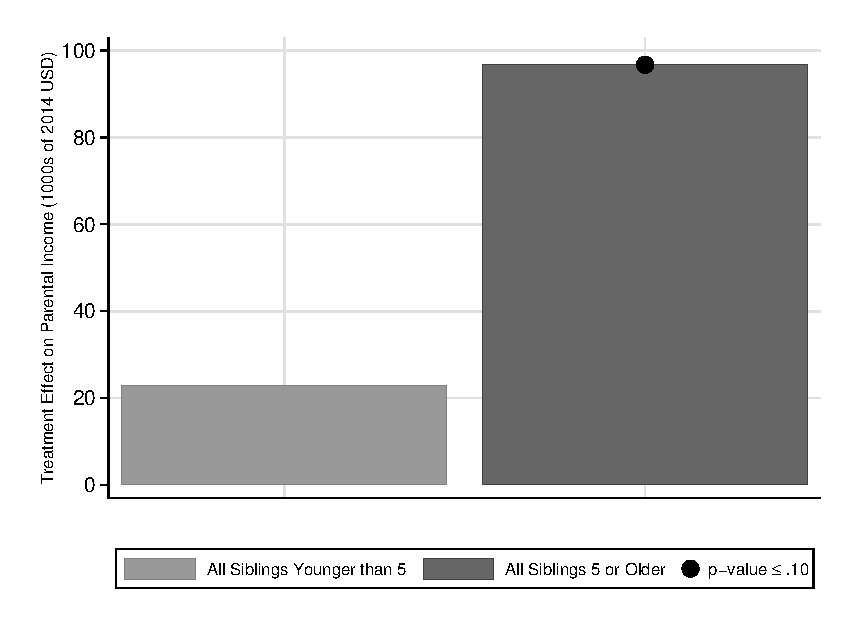
\includegraphics[width=\textwidth]{output/abccare_pincomesumsibage_spooled.eps}
\end{subfigure}
\footnotesize \justify
Note: Panel (a) displays the net-present value (treatment less control) of parental income of parents of children with and without siblings at baseline. Panel (b) displays the average parental income of parents of children with young siblings (younger than 5 years old) and children with older siblings (5 years old or older) at baseline. Panel (b) drops children without siblings at baseline. Parental income is in 2014 USD discounted to child's participant age 0 using a 3\% rate. We use the baseline ``conservative'' measure of parental income in Section~\ref{section:pincome}. Results using our alternative parental income measures are similar (see Appendix~\ref{app:parentalincome}).
\end{figure}

\paragraph{Using Mincer Equations to Predict Parental Income} \label{appendix:mincerpar}

\noindent This approach fits Mincer regressions for parental income.\footnote{See \citet{Mincer_1974_schooling} for the original source and \citet{Heckman_Lochner_ea_2006_HEE} for a extended discussion of the Mincer equation, its implications, and several extensions.} We specify how we deal with the presence of a spouse below. The parameterization used is as follows:

\begin{equation}
\ln Y_{a} = \alpha + \beta \cdot \text{school}_{a} + \gamma_{1}  \cdot \text{experience}_{a} + \gamma_{2} \cdot {\text{experience}_{a}}^2 + \bm{\psi} \mathbf{X}_{a} + \eta_{a}, \label{eq:mincer}
\end{equation}

\noindent where variables are indexed by mother's age, $\ln Y_a$ is log-labor income at age $a$, experience and schooling are measured in years, $ \mathbf{X}_{a}$ are observed characteristics, and $\eta_{a}$ is an unobserved component. $\alpha, \beta, \gamma_{1}, \gamma_{2}, \bm{\psi}$ are coefficients and summarize the parameterization of the labor income profile.\footnote{We assign one dollar of income when parental income is reported to be zero.}\\

\noindent In principle, there is no reason why the parameters characterizing the profile should differ across the treatment and control groups in ABC/CARE. Given the small sample in ABC/CARE, we assume that the profile is common across the control and treatment groups. This assumption is analogous to Assumption~\ref{ass:summary}, which we fail to reject in Appendix~\ref{app:invariance}.\\

\noindent We estimate the coefficients in \eqref{eq:mincer} using the sample of mothers in ABC/CARE. We pool the longitudinal information and estimate the coefficients using ordinary least squares. We use a standard Mincer measure of experience (age - education - 6). We assign one dollar to mothers with no labor income. For mothers living with a working partner, we allocate $1/2$ of total parental income as $Y_{a}$. To validate our estimates within ABC/CARE, we estimate the coefficients \eqref{eq:mincer} using a sub-sample of disadvantaged mothers in the PSID.\footnote{We define disadvantaged as follows: Black, not married, labor income, education (at age 5 of child's participant), age and number of children (at age 5 of child's participant) in the same ranges as the ABC/CARE mothers, labor income below percentile 75.} The coefficients characterizing \eqref{eq:mincer} in ABC/CARE and PSID for different combinations of control sets are in agreement. We display them in Table~\ref{table:mincerpsid}.\\

\begin{table}[H]
\begin{threeparttable}
\caption{Mincer Equation Estimates for Mothers in ABC/CARE and the PSID}
\label{table:mincerpsid}
\centering
\footnotesize
\begin{tabular}{lcccccc} \toprule
 & PSID & ABC/CARE & PSID & ABC/CARE & PSID & ABC/CARE \\ \midrule
Education & 0.0762*** & 0.0614*** & 0.1155*** & 0.1000*** & 0.1109*** & 0.0852*** \\
 & (0.0050) & (0.0161) & (0.0057) & (0.0151) & (0.0057) & (0.0184) \\
Experience &  &  & 0.0386*** & 0.0908*** & 0.0417*** & 0.0861*** \\
 &  &  & (0.0027) & (0.0086) & (0.0027) & (0.0085) \\
Experience$^2$ &  &  & -0.0005*** & -0.0018*** & -0.0007*** & -0.0015*** \\
 &  &  & (0.0001) & (0.0003) & (0.0001) & (0.0003) \\
Birth Year &  &  &  &  & -0.0041*** & 0.0104 \\
 &  &  &  &  & (0.0008) & (0.0084) \\
Children &  &  &  &  & -0.0803*** & -0.0533 \\
 &  &  &  &  & (0.0068) & (0.0372) \\
Constant & 8.2789*** & 8.8869*** & 7.3572*** & 7.8229*** & 15.6408*** & -12.3540 \\
 & (0.0609) & (0.1892) & (0.0780) & (0.1895) & (1.5533) & (16.6026) \\ \midrule
Observations & 15,506 & 705 & 15,506 & 705 & 15,506 & 664 \\
$R^2$ & 0.0145 & 0.0194 & 0.0416 & 0.2215 & 0.0514 & 0.2047 \\ \bottomrule
\end{tabular}

\begin{tablenotes}
\footnotesize
\item Note: This table presents estimates of \eqref{eq:mincer} for ABC/CARE mothers and a subsample of disadvantaged mothers in the PSID. We define disadvantaged as follows: Black, not married, labor income, education (at age 5 of child's participant), age and number of children (at age 5 of child's participant) in the same ranges as the ABC/CARE mothers, labor income below percentile 75. Robust standard errors are in parentheses. $p$-value $< .01$. $^{**}$: $p$-value $< .05$. $^{*}$: $p$-value $< .10$.
\end{tablenotes}
\end{threeparttable}
\end{table}

\noindent Based on the estimates in Table~\ref{table:mincerpsid}, we can ask two questions: (i) what is the predicted net present value of parental income (treatment - control) using a prediction based on the estimate of \eqref{eq:mincer} and how does it differ from the method that linearly interpolates income from child's age 0 to 21?; and (ii) what would be the predicted net present value of parental income if we go beyond and predict all the way up to 40 years of experience?\\

\noindent Table~\ref{table:psens} display results that answer these two questions. Precise estimates for \eqref{eq:mincer} are obtained. From it we can measure (treatment - control) when the subjects are 21 years old. When using these same equations to predict parental labor income such that mothers work for 40 years in their life times, we find that we add $\$30,000$ (2014 USD) to the estimate reported in the main paper.

\begin{table}[H]
\begin{threeparttable}
\caption{Parental Labor Income, Interpolations and Prediction}
\label{table:psens}
\centering
\begin{tabular}{lccc} \toprule
 & Males and Females  & Male  & Female  \\  \midrule
 Interpolated up to Age 21 & 82,287 & 65,477 & 96,251 \\
 & (22,981.46) & (26,603.57) & (32,000.64) \\
Mincer-based up to Age 21 &  75,114 &  72,030 &  78,198 \\  
 & (428.340) & (647.017) & (557.716) \\  
Mincer-based up to Retirement &  106,957 &  102,556 &  111,338 \\  
 & (609.870) & (921.222) & (794.076) \\  
\bottomrule \end{tabular} 

\begin{tablenotes}
\footnotesize
\item Note:  Interpolated up to Age 21: linearly interpolated parental income from (child's) age 0 to 21. Mincer-based up to Age 21: prediction from (child's) age 0 to 21 based on estimates coefficients of \eqref{eq:mincer} (full control set). Mincer-based up to Retirement: prediction from (child's) age 0 to mother's retirement (40 years of labor force participation assumed) based on estimates coefficients of \eqref{eq:mincer} (full control set). All values are in 2014 USD discounted to child's age 0. Standard errors in parentheses are based on the empirical bootstrap distribution.
\end{tablenotes}
\end{threeparttable}
\end{table}

\paragraph{Life-cycle Prediction of Parental Income} \label{appendix:lcyclepincome}

\noindent The third approach is to predict parental income as in Section~\ref{section:cbamethodology}. For want of maternal characteristics enabling us to construct synthetic treatment and control groups, we skip the matching procedure and directly implement the prediction. That is, we do not construct a synthetic control and treatment groups to fit the dynamic relationships in the auxiliary samples. Instead, we assume that all parental income is earned by the mother and limit the sample to Black females whose labor income at each age is below the in-sample 90th percentile (we calculate this for the PSID and NLSY79 separately before using them jointly as one sample). As with labor income (of program participants) after age 30, we use the PSID and NLSY79 as one sample. For the same lack of data, we use a single predictor: lagged parental income. We initialize the prediction with the last observed measure of maternal income and extrapolate until the mother is 65 years old. Figure~\ref{figure:pincomeapp} displays our estimate of parental income in a format similar to Figure~\ref{figure:pincome}.\\

\begin{figure}[!htbp]
\centering
\caption{Discounted Net-present Value of Parental Income by Participant's Number and Age of Siblings at Baseline}\label{figure:pincomeapp}
\begin{subfigure}[h]{0.5\textwidth}
		\centering
		\caption{No Siblings vs. $>0$ Siblings}
		\includegraphics[width=\textwidth]{output/abccare_pinc_npv_pooled.eps}
\end{subfigure}%
\begin{subfigure}[h]{0.5\textwidth}
		\centering
		\caption{Siblings Younger than 5 vs. Siblings 5 or Older}
		\includegraphics[width=\textwidth]{output/abccare_pinc_npv_sibs5_pooled.eps}
\end{subfigure}
\footnotesize \justify
Note: Panel (a) displays the net-present value (treatment less control) of parental income of parents of children with and without siblings at baseline. Panel (b) displays the average parental income of parents of children with young siblings (younger than 5 years old) and children with older siblings (5 years old or older) at baseline. Panel (b) drops children without siblings at baseline. Parental income is in 2014 USD discounted to child's participant age 0 using a 3\% rate.  We use the measure of parental income in Section~\ref{section:pincome}.
\end{figure}

\noindent \textbf{Summary: Prediction of Parental Labor Income}\\
\noindent Any prediction of parental income starts at the last observation of parental income, which varies by individual due to attrition. For prediction, we assume that parental income is equal to maternal income (only 27\% of mothers in ABC/CARE report leaving with a couple).
\begin{enumerate}
\item \textbf{Mincer Model}
\begin{enumerate}
\item \textbf{Auxiliary Sample Used to Predict:} PSID.
\item \textbf{Initial Restrictions Placed on the Auxiliary Sample:} Black; female; unmarried; education and number of children at ages 5 in the ranges of ABC/CARE participants, labor income at each age is below the 75th percentile.
\item \textbf{Variables Used to Construct Synthetic Control and Treatment Groups:} we pool PSID/NLSY79 restricted sample, and do not construct synthetic experimental groups due to lack of variables to do so.
\item \textbf{Variables Used to Predict:} education, second order polynomial in experience, birth year, number of children.
\item \textbf{Assumed Retirement:} after 40 years of labor force participation.
\end{enumerate}
\item \textbf{Life-cycle Prediction}
\begin{enumerate}
\item \textbf{Auxiliary Sample Used to Predict:} PSID and NLSY79.
\item \textbf{Initial Restrictions Placed on the Auxilliary Sample:} Black; female; labor income at each age is below the 90th percentile.
\item \textbf{Variables Used to Construct Synthetic Control and Treatment Groups:} we pool the PSID restricted sample, and do not construct synthetic experimental groups due to lack of variables to do so.
\item \textbf{Variables Used to Predict:} lagged labor income.
\item \textbf{Assumed Retirement:} 65 years old.
\end{enumerate}
\end{enumerate}

\subsection{Internal Rate of Return}
\label{app:method_irr}

\noindent To estimate the internal rate of return, we solve for $\rho$ in the following equation:
\begin{align}
\sum_{a=0}^A \frac{ \mathbb{E} (B_a - C_a)}{(1+\rho)^a} = 0,
\end{align}
where we let $A = 79$, define $B_a$ and $C_a$ to be the (discounted) total benefits and costs of the program at age $a$, and define $\mathbb{E}(.)$ to be the sample mean.\footnote{This is an abuse of notation given that $B_a$ and $C_a$ are not discounted in Appendix~\ref{app:method_irr}.} That is, we estimate the internal rate of return for the \textit{average subject} of ABC/CARE. \\

\noindent All outcomes of the parents and subjects affected by the program are treated as benefits. For this to make sense, we reverse the sign of the monetized effect of the program on specific outcomes. Costs of ABC/CARE consist only of the initial program costs from ages 0 to 5. Table \ref{table:bc_comp} provides a full list of the benefits and costs of ABC. \\

\noindent We take the sum of the treatment effects on each component of the benefits to be the total benefit, $B_a$, of the ABC/CARE program. This includes parental income, subject labor income, and QALYs (quality-adjusted life years). Treatment effects on costs borne by the subject or society have their signs reversed and are included as benefits. We do this for subject public-transfer income, education costs, crime costs, control substitution costs, and health costs. To account for deadweight loss, we impose a marginal welfare cost of 50\% by multiplying public costs by a factor of $0.5$ when they are a direct transfer from the government to the individuals\footnote{There is no clear consensus on the marginal welfare cost of tax revenue. However, most researchers estimate the welfare cost per tax dollar to be between \$0.30 and \$0.50. See \citet{Feldstein_1999_REStat}, \citet{Heckman_Smith_1998_evaluating}, and \citet{Browning_1987_AER}.} When the public costs are not a direct transfer from the government to the individuals, we multiply them by a factor of $1.5$.\\

\noindent The principle for multiplying the public costs is the following. We evaluate the social benefits of ABC/CARE and do not place a value on who receives the money. The only social cost from a direct transfer is the dead-weight loss that it generates: $50\%$ of its total value. We do not consider education and criminal costs to be a direct transfer. Thus, we multiply them by a factor of $1.5$: the value of their cost plus $50\%$ of the value of their cost (the dead-weight loss implied in raising the public revenue to fund them). Table \ref{table:bc_comp} lists the factor we use to multiply each cost to account for its implied dead-weight loss.\\

\noindent Having constructed our cash flow, $\mathbb{E} (B_a - C_a)$, solving for $\rho$ reduces to an algebraic exercise. The expected life-cycle profile of net benefits need to satisfy a ``single crossing property'' in order to obtain a unique solution for the internal rate of return.\footnote{See \citet{Arrow-Levhari_1969_EJ} for a formal discussion, although the discussion on multiplicity, sign, and real or complex nature of the roots of a polynomial traces back to Descarte's Rule.} The single crossing property holds when the benefits do not go from positive to negative across the life cycle. When the single crossing property is not satisfied, the internal rate of return is not a valid summary for the efficiency of an investment. To calculate the internal rate of return, we estimate the treatment effect on each component of the benefits and costs at age $a$ for the pooled, male, and female samples. We do this for 100 bootstrap resamples of the original ABC/CARE data. In the case of health costs and subject income, for which we employ auxiliary datasets to estimate the treatment effects, we also obtain 100 bootstrap estimates from the auxiliary data for every ABC/CARE bootstrap resample, resulting in a total of 100,000 estimates. By reusing each bootstrap estimate of the treatment effect on outcomes that do not require any auxiliary data set 100 times, we obtain a total of 100,000 estimates of the cash flow. We estimate the internal rate of return on each of those cash flows, and discard those for which we find a negative internal rate of return. The remaining estimates form our empirical bootstrap distribution of the internal rate of return for the pooled, male, and female samples. We take the mean of the distributions to be the point estimates, and we take the sample standard deviations to be the standard errors. To construct the 80\% confidence intervals, we take the 10\textsuperscript{th} and 90\textsuperscript{th} quantiles of each bootstrap distribution.\\

\noindent Figure~\ref{figure:irrdist} reports the distributions of the internal rates of return, by gender and for each of the three parameters that we consider (treatment vs. next best, treatment staying at home, treatment vs. alternative preschool). For some parameters and genders, we discard a high percentage of the internal rate of return of the outcomes. We next discuss how we calculate the benefit/cost ratios, noting that this statistics is not subject the same caveat as the internal rate of return: we can summarize the efficiency of the investment even in the absence of the single-crossing property.

\newgeometry{top=.6in, bottom=.8in, left=.6in, right=.6in}
\begin{sidewaysfigure}[!htbp]
\centering
\caption{Internal Rate of Return, by Gender and by Parameter}\label{figure:irrdist}
\begin{subfigure}[h]{0.25\textwidth}
		\centering
		\caption{Treatment vs. Next Best, Pooled}
		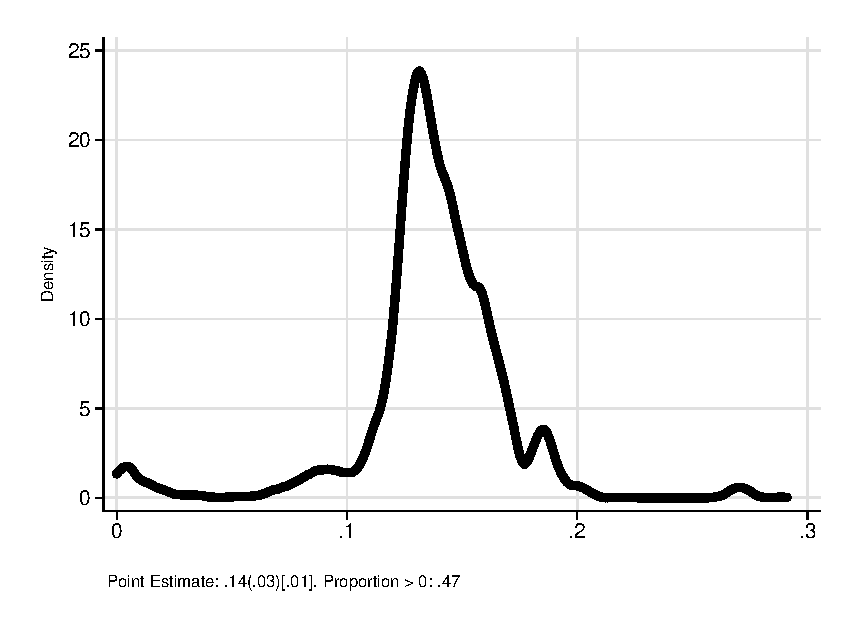
\includegraphics[width=\textwidth]{output/irr_2_sexp.eps}
\end{subfigure}%
\begin{subfigure}[h]{0.25\textwidth}
	\centering
	\caption{Treatment vs. Next Best,\\ Females}
		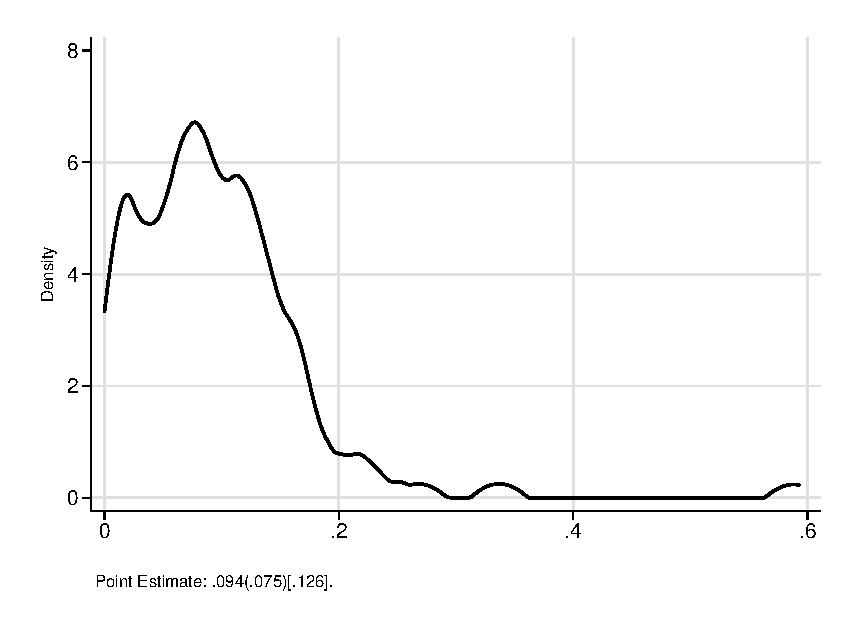
\includegraphics[width=\textwidth]{output/irr_2_sexf.eps}
\end{subfigure}%
\begin{subfigure}[h]{0.25\textwidth}
		\centering
		\caption{Treatment vs. Next Best, Males}
		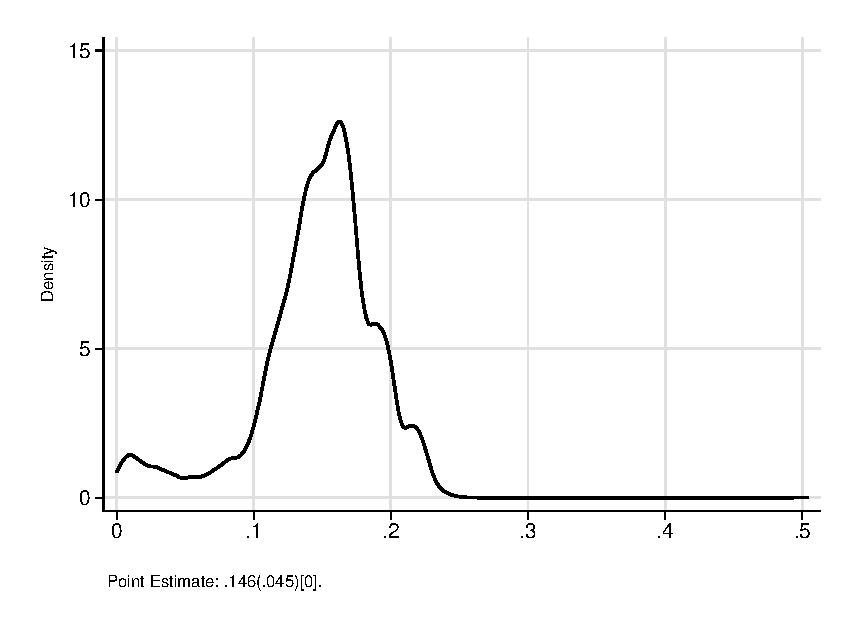
\includegraphics[width=\textwidth]{output/irr_2_sexm.eps}
\end{subfigure}
\begin{subfigure}[h]{0.25\textwidth}
	\centering
	\caption{Treatment vs. Staying at Home, Pooled}
		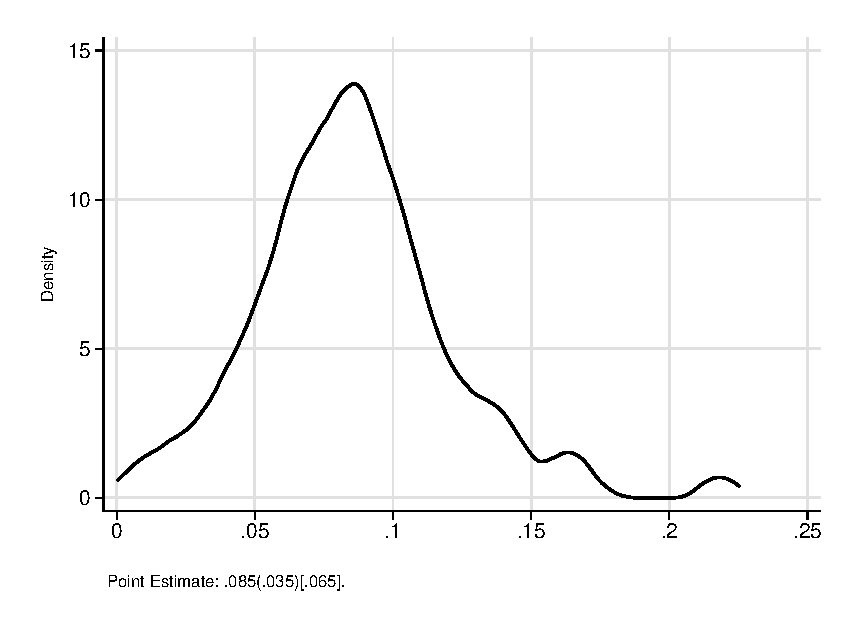
\includegraphics[width=\textwidth]{output/irr_5_sexp.eps}
\end{subfigure}%
\begin{subfigure}[h]{0.25\textwidth}
	\centering
	\caption{Treatment vs. Staying at Home, Females}
		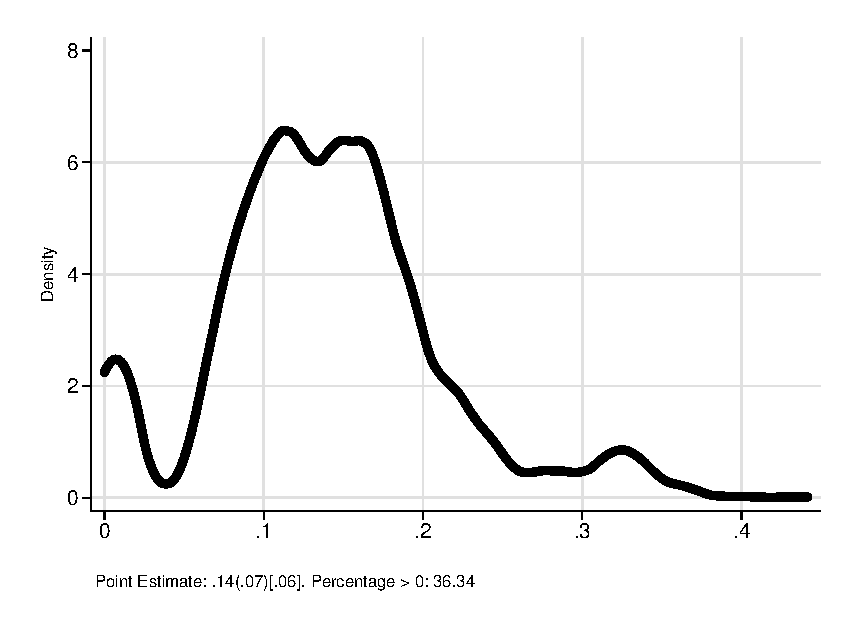
\includegraphics[width=\textwidth]{output/irr_5_sexf.eps}
\end{subfigure}%
\begin{subfigure}[h]{0.25\textwidth}
	\centering
	\caption{Treatment vs. Staying at Home, Males}
		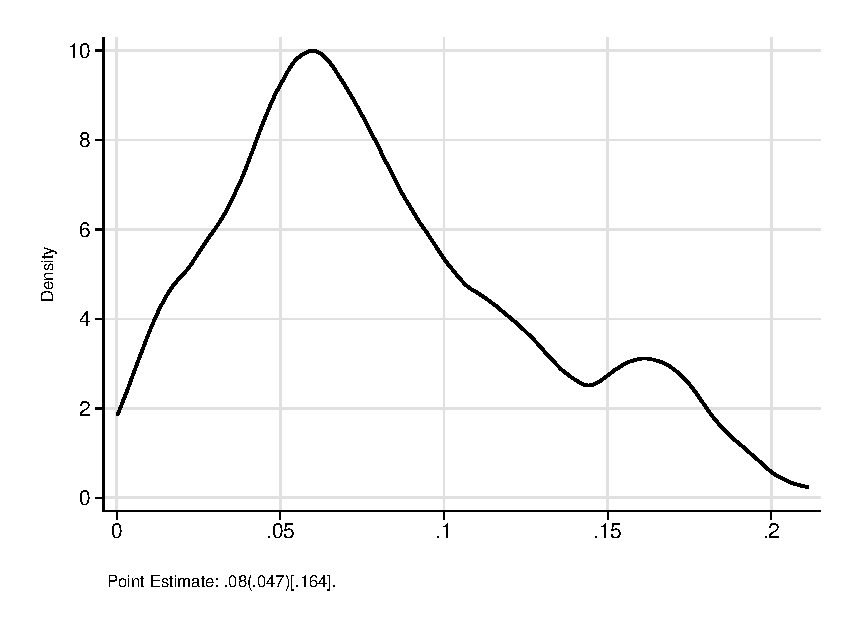
\includegraphics[width=\textwidth]{output/irr_5_sexm.eps}
\end{subfigure}
\begin{subfigure}[h]{0.25\textwidth}
	\centering
	\caption{Treatment vs. Alternative Preschool, Pooled}
		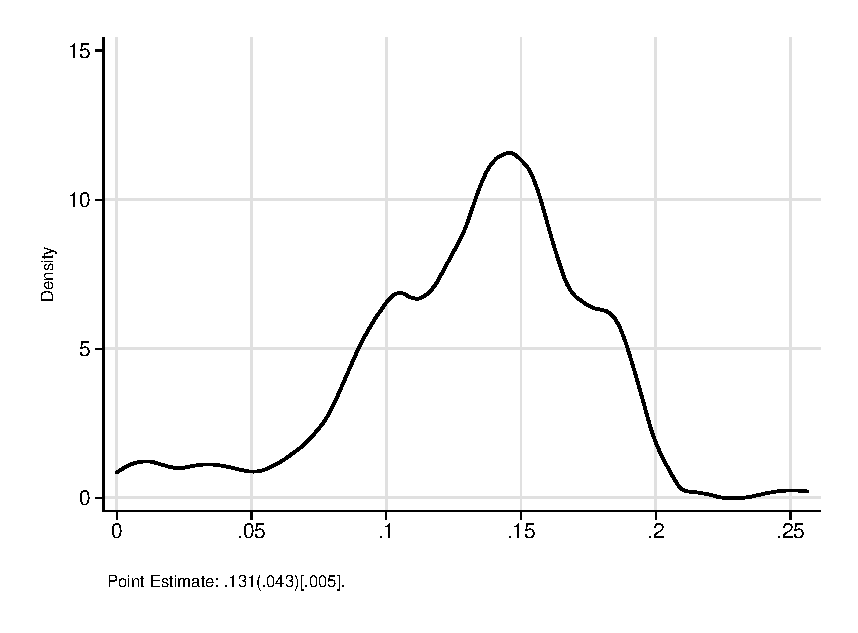
\includegraphics[width=\textwidth]{output/irr_8_sexp.eps}
\end{subfigure}%
\begin{subfigure}[h]{0.25\textwidth}
	\centering
	\caption{Treatment vs. Alternative Preschool, Females}
		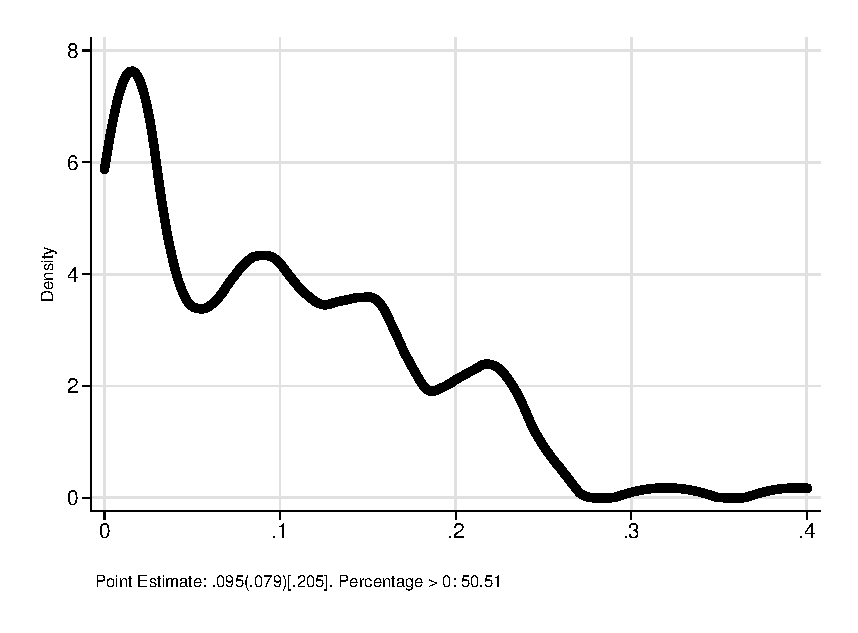
\includegraphics[width=\textwidth]{output/irr_8_sexf.eps}
\end{subfigure}%
\begin{subfigure}[h]{0.25\textwidth}
	\centering
	\caption{Treatment vs. Alternative Preschool, Males}
		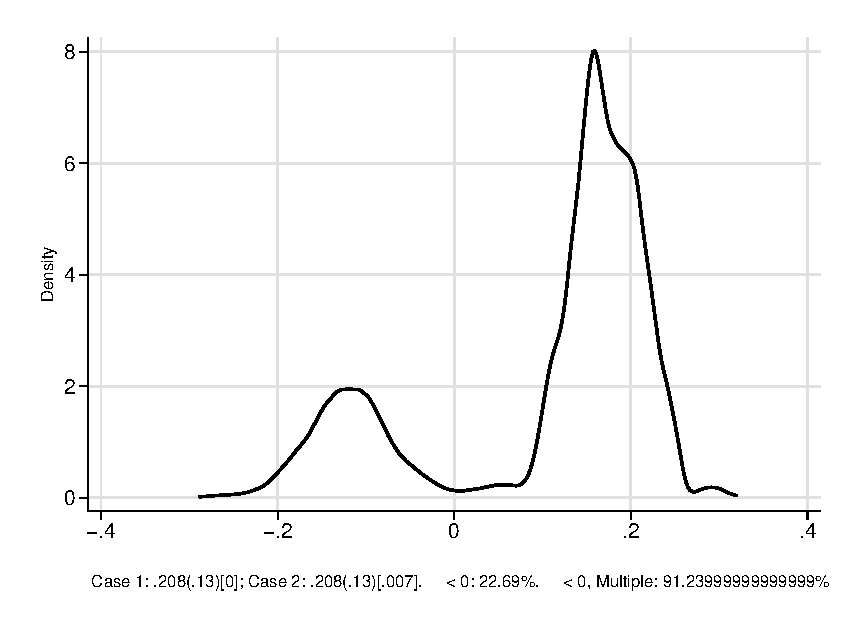
\includegraphics[width=\textwidth]{output/irr_8_sexm.eps}
\end{subfigure}
\footnotesize \justify
Note: Panel (a) displays the empirical bootstrap distribution for the estimate of the treatment vs. next parameter in the pooled sample. The reminder panels show an analogous distribution varying the parameter and the gender. See Section~\ref{section:methodsquestions} for the definition of the parameters. We discard negative internal rates of returns. Each panel displays the point estimate with the standard error in parentheses and the $p$-value in brackets in the left corner and the percentage of positive internal rates of return out of the initial set of bootstrap resamples in the right corner.
\end{sidewaysfigure}
\restoregeometry
\doublespacing



% We let $T = 79$. In Appendix \ref{app:method_identify}
% we explain how we can estimate the summand of the numerator at every period $t$, which
% can be expressed as $\mathbf{E}(B_t) -  \mathbf{E}(C_t)$. Thus, solving for $\rho$
% reduces to an algebraic exercise.



% To construct our cash flow, we subtract the costs from benefits to create a single stream.
% We define `cost' to include only the program costs of ABC, and define
% `benefits' to include all treatment effects of the program. This includes
% the treatment effects on parent income, subject labor income, and QALY
% (quality adjusted life years).\footnote{QALYs are measured on a scale of 0 to 1, with 1 being a
% year of perfect health. We follow \textbf{[CITATION]} and value a QALY of 1 to be
% \$150,000, and a QALY of 0 to be \$0. The dollar value of that year relates linearly to the QALY.}
% Treatment effects on costs borne by the subject or society have their signs
% reversed and are included as benefits. We do this for subject transfer income,
% education costs, jail costs, justice system costs, victimization costs,
% control contamination costs, and medical costs. To account for deadweight loss, we
% impose a marginal welfare cost of 50\% by multiplying public costs by a factor of
% $1.5$.\footnote{There is no clear consensus on the marginal welfare cost of tax revenue. However,
% most researchers estimate the welfare cost per tax dollar is between \$0.30--0.50. See
% \citet{feldstein1999tax, heckman1998evaluating, browning1987marginal}.} This
% includes education cost up until age 17, jail costs, justice system costs, Medicare costs,
% and Medicaid costs. For the same reason, we multiply transfer income by a factor of 0.5.

% For each period $t \in \{1, 2, \dots, 79\}$, we sum our estimates of the benefits, and
% subtract our estimates of the costs from that sum. This provides us an estimate of
% $\mathbf{E}(B_t) -  \mathbf{E}(C_t) = \mathbf{E} (B_t - C_t)$. We then solve for
% $\rho$ using numerical analysis.

% In your methodlogy you describe costs and benefits differnetly....
% To construct our cash flow, we sum the costs and benefits from the program into a single stream.
% We define `cost' to include only the cost of implementing ABC. On the other hand,
% we broadly define `benefits' to include all treatment effects of the program. This includes
% the treatment effects on parent income, subject labor income, and QALY
% (quality adjusted life years).\footnote{QALYs are measured on a scale of 0 to 1, with 1 being a
% year of perfect health. We follow \textbf{[CITATION]} and value a QALY of 1 to be
% \$150,000, and a QALY of 0 to be \$0. The dollar value of that year relates linearly to the QALY.}
% Treatment effects on outcomes generally considered to be costs have their signs reversed in
% order to convert them into benefits. We do this for subject transfer income,
% education costs, jail costs, justice system costs, victimization costs,
% control contamination costs, and medical costs. To account for deadweight loss, we
% impose a marginal welfare cost of 50\% by multiplying public costs by a factor of
% $1.5$.\footnote{There is no clear consensus on the marginal welfare cost of tax revenue. However,
% most researchers estimate the welfare cost per tax dollar is between \$0.30--0.50. See
% \citet{feldstein1999tax, heckman1998evaluating, browning1987marginal}.} This
% includes education cost up until age 17, jail costs, justice system costs, Medicare costs,
% and Medicaid costs. For the same reason, we multiply transfer income by a factor of 0.5.


\subsection{Computing the Benefit/Cost Ratio}\label{app:method_cbratio}

\noindent The benefit/cost ratio is
\begin{align}
\mathbb{E} \left( \frac{ \sum_{a=0}^A B_a}{\sum_{a=0}^A C_a} \right),
\end{align}

\noindent where we let $A = 79$, define $B_a$ and $C_a$ to be the benefits and costs of the
program at age $a$, and define $\mathbb{E}(.)$ to be the sample mean. See Table \ref{table:bc_comp} for a detailed list of the components
to the benefits and costs of ABC/CARE . We take the sum of the treatment effects on each component
of the benefits to be the total benefits of the ABC/CARE programs. \\

\noindent To account for deadweight loss, we assume a marginal welfare cost of 50\% by multiplying
public costs components by a factor of $1.5$. For the same reason, we multiply public-transfer
income by a factor of 0.5. We discount each component of the benefits and costs
by 3\% every year to obtain their net present value at birth. We then sum up the discounted
components of the benefits and find the ratio with the discounted costs. \\

\noindent We estimate the treatment effect for each component of the benefits and costs at age $a$ for the pooled, male, and female samples. We do this for 100 bootstrap resamples of the original ABC/CARE data. In the case of health and subject income, for which we employ auxiliary datasets to estimate the treatment effects, we also obtain 100 bootstrap estimates from the auxiliary data for every ABC/CARE bootstrap resample, resulting in a total of 100,000 estimates. By reusing each bootstrap estimate of the treatment effect on outcomes that do not require any auxiliary data set 100 times, we obtain a total of 100,000 estimates of the costs stream and benefits stream. We estimate the benefit/cost ratio for each of those streams. This is how we form our empirical bootstrap distribution of the benefit/cost ratio for the pooled, male, and female samples. We take the mean of the distributions to be the point estimates, and we take the standard deviations to be the standard errors. To construct the 80\% confidence intervals, we take the 10\textsuperscript{th} and 90\textsuperscript{th} quantiles of each bootstrap distribution. Figure~\ref{figure:ratiodist} presents the empirical distribution of the empirical bootstrap distribution, per parameter of interest and gender.

\begin{table}[H]
\begin{threeparttable}
\caption{Components of Benefits and Costs}
\label{table:bc_comp}
\centering
\begin{tabular}{l l p{2cm}}
\hline\hline			
Variable & Sign Reversed	& Welfare Cost Factor \\
\hline
\emph{Benefits} 	\\			
Parent Income			& No \\
Subject QALY			& No \\
Subject Labor Income	& No \\
Subject Transfer Income	& Yes	& 0.5 \\
Medicare Costs			& Yes	& 1.5 \\
Medicaid Costs			& Yes	& 1.5 \\
Out-of-pocket Medical Costs	& Yes \\
Miscellaneous medical Costs	& Yes \\
Disability Insurance Claim	& Yes	&	1.5 \\
Social Security Claim	& Yes	&	1.5 \\
Supplemental Security Claim	& Yes	&	1.5 \\
Control Contamination Costs	& Yes	& \\
Education Costs			& Yes	& 1.5$^{*}$ \\
Justice System Costs	& Yes	& 1.5 \\
Prison Costs			& Yes	& 1.5 \\
Victimization Costs		& Yes	& \\
\\
\emph{Costs} 	\\			
Program Costs			& No \\
\hline\hline			
\end{tabular}
\begin{tablenotes}
\footnotesize
\item Note: The table lists the components of the costs and benefits of ABC/CARE.
In order for some components to be categorized as benefits, we reversed the sign
of the treatment effect. *Only education costs up until age 18 are multiplied by 1.5 to account for welfare costs. This factor is drawn from \citet{Heckman_Moon_etal_2010_RateofReturn}.
\end{tablenotes}
\end{threeparttable}
\end{table}

\newgeometry{top=.6in, bottom=.8in, left=.6in, right=.6in}
\begin{sidewaysfigure}[!htbp]
\centering
\caption{Benefit/Cost Ratios, by Gender and by Parameter}\label{figure:ratiodist}
\begin{subfigure}[h]{0.25\textwidth}
		\centering
		\caption{Treatment vs. Next Best, Pooled}
		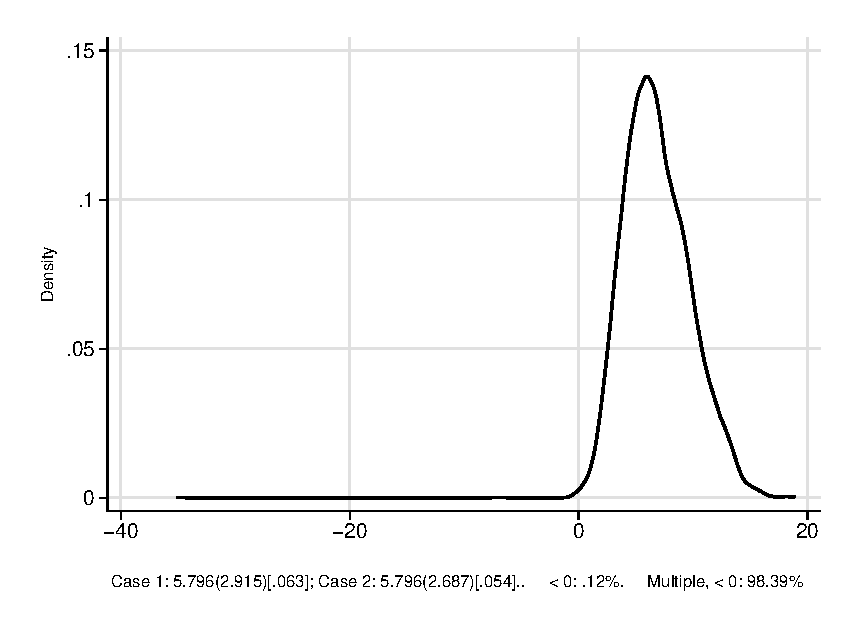
\includegraphics[width=\textwidth]{output/ratios_2_sexp.eps}
\end{subfigure}%
\begin{subfigure}[h]{0.25\textwidth}
	\centering
	\caption{Treatment vs. Next Best,\\ Females}
		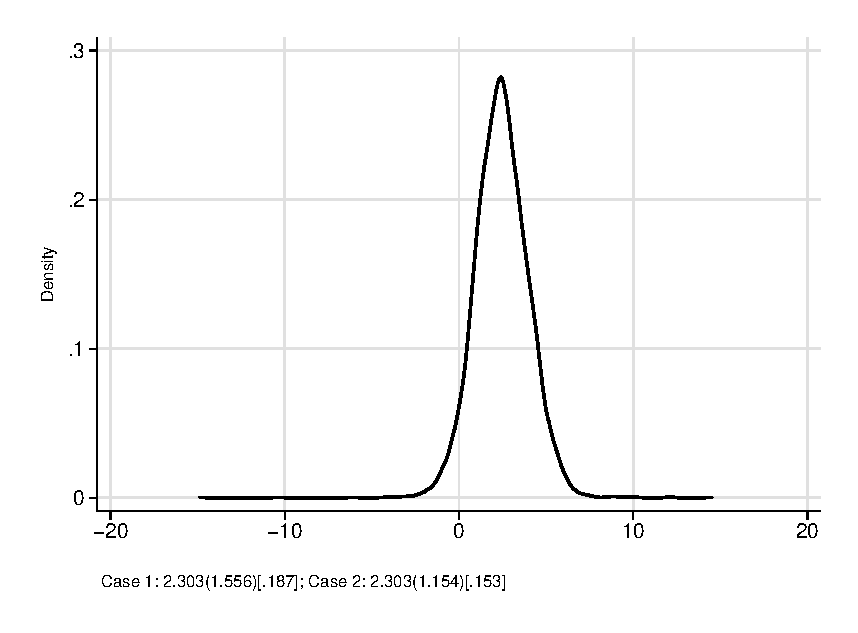
\includegraphics[width=\textwidth]{output/ratios_2_sexf.eps}
\end{subfigure}%
\begin{subfigure}[h]{0.25\textwidth}
		\centering
		\caption{Treatment vs. Next Best, Males}
		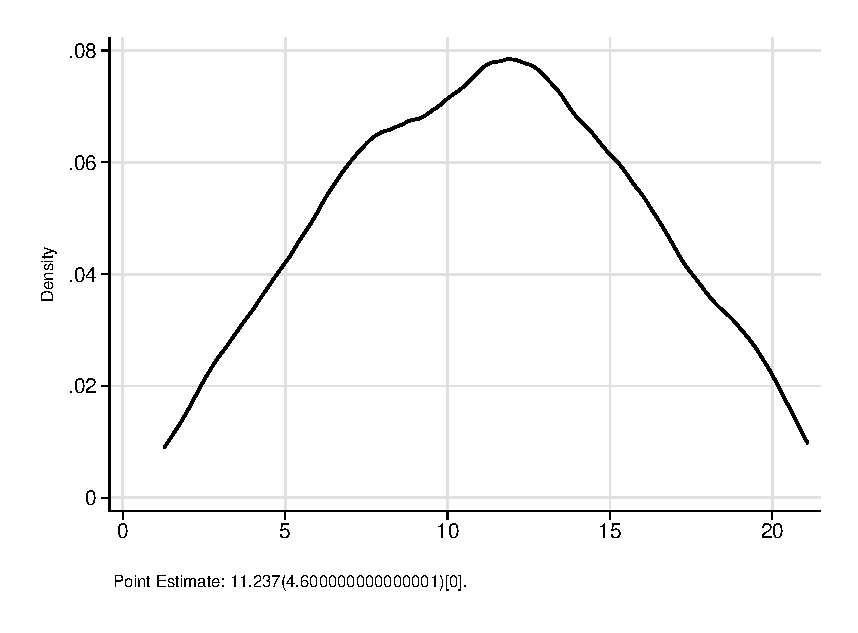
\includegraphics[width=\textwidth]{output/ratios_2_sexm.eps}
\end{subfigure}
\begin{subfigure}[h]{0.25\textwidth}
	\centering
	\caption{Treatment vs. Staying at Home, Pooled}
		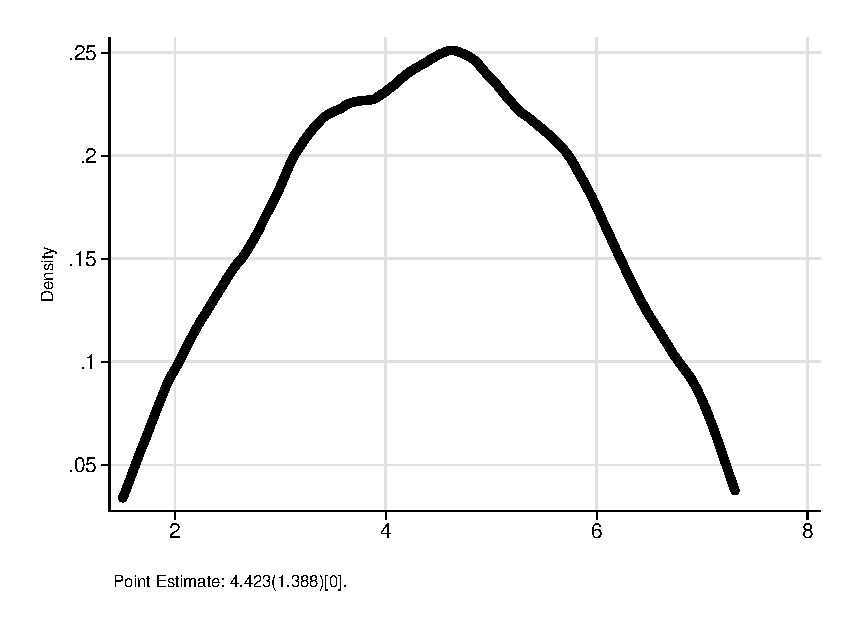
\includegraphics[width=\textwidth]{output/ratios_5_sexp.eps}
\end{subfigure}%
\begin{subfigure}[h]{0.25\textwidth}
	\centering
	\caption{Treatment vs. Staying at Home, Females}
		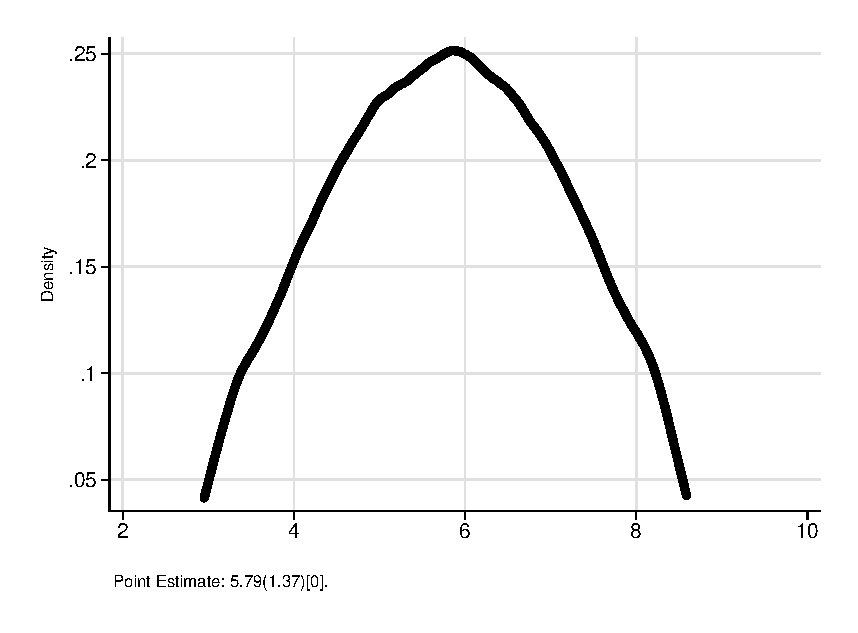
\includegraphics[width=\textwidth]{output/ratios_5_sexf.eps}
\end{subfigure}%
\begin{subfigure}[h]{0.25\textwidth}
	\centering
	\caption{Treatment vs. Staying at Home, Males}
		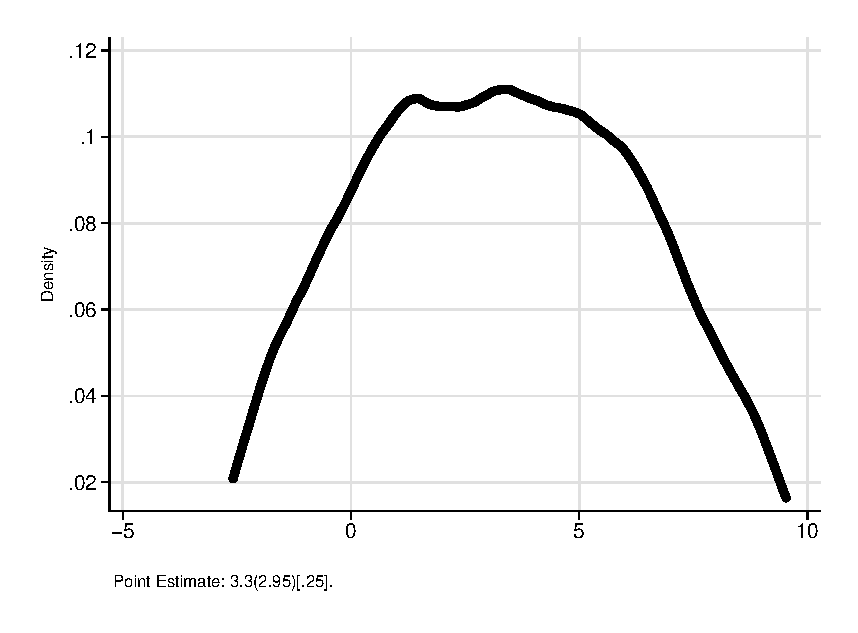
\includegraphics[width=\textwidth]{output/ratios_5_sexm.eps}
\end{subfigure}
\begin{subfigure}[h]{0.25\textwidth}
	\centering
	\caption{Treatment vs. Alternative Preschool, Pooled}
		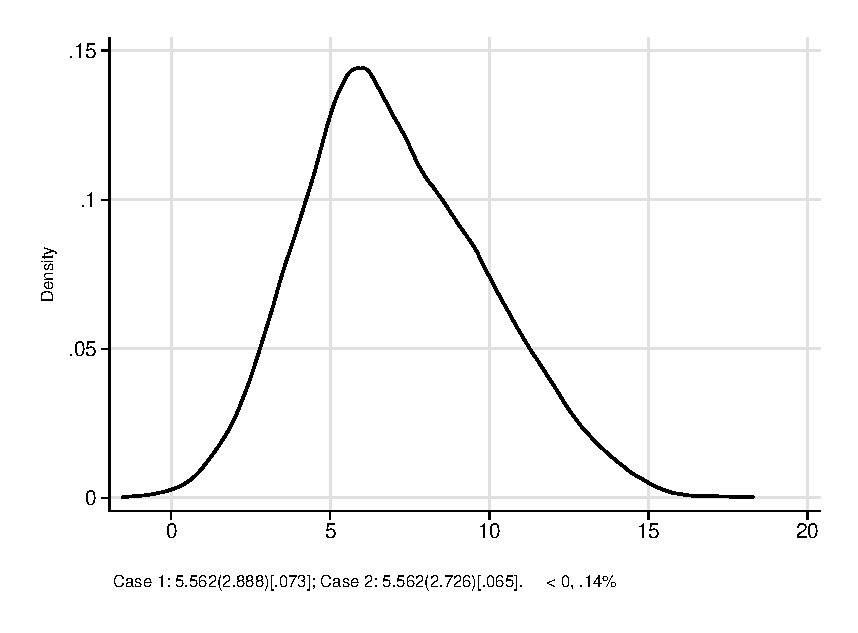
\includegraphics[width=\textwidth]{output/ratios_8_sexp.eps}
\end{subfigure}%
\begin{subfigure}[h]{0.25\textwidth}
	\centering
	\caption{Treatment vs. Alternative Preschool, Females}
		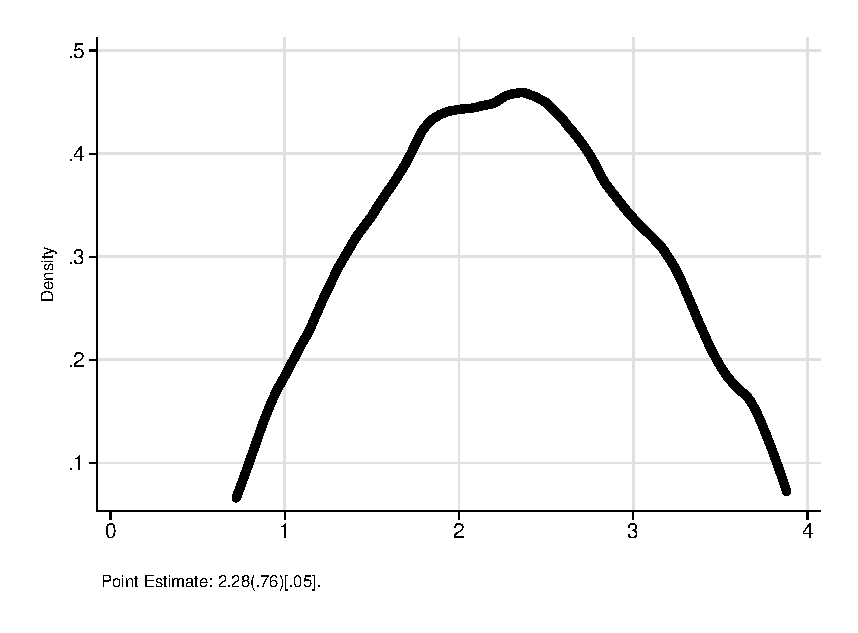
\includegraphics[width=\textwidth]{output/ratios_8_sexf.eps}
\end{subfigure}%
\begin{subfigure}[h]{0.25\textwidth}
	\centering
	\caption{Treatment vs. Alternative Preschool, Males}
		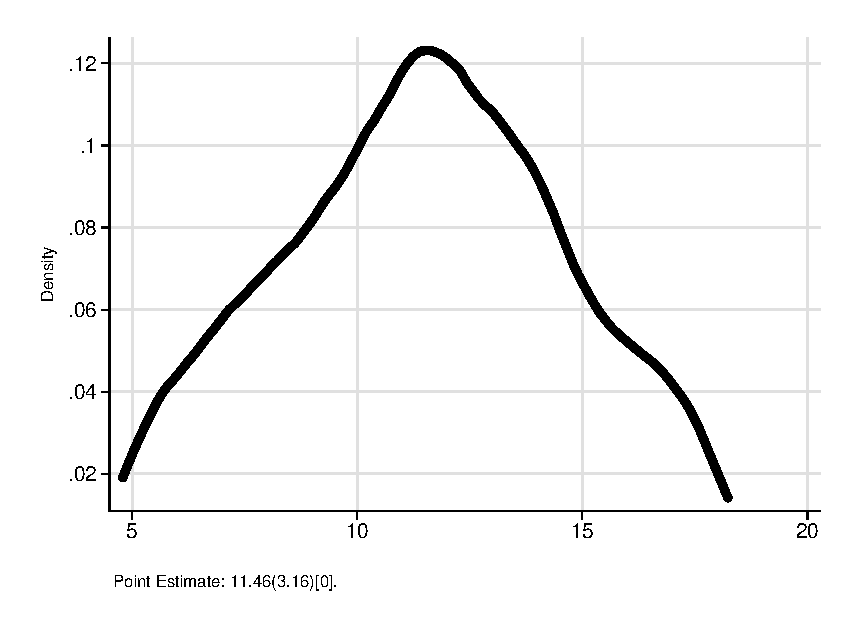
\includegraphics[width=\textwidth]{output/ratios_8_sexm.eps}
\end{subfigure}
\footnotesize \justify
Note: Panel (a) displays the empirical bootstrap distribution for the estimate of the treatment vs. next parameter in the pooled sample. The reminder panels show an analogous distribution varying the parameter and the gender. See Section~\ref{section:methodsquestions} for the definition of the parameters. Each panel displays the point estimate with the standard error in parentheses and the $p$-value in brackets in the left corner.
\end{sidewaysfigure}
\restoregeometry
\doublespacing

\subsection{Exploring the Impact of Using Different Prediction Models} \label{appendix:predsensitivity}
\noindent \textbf{[JLG: All your requests to this section have been completed.]}\\

\noindent Our analysis is based on a causal model for treatment ($d=1$) and control ($d=0$) outcomes for measure $j$ at age $a$ in sample $k \in \{e,n\}$ where $e$ denotes membership in the experimental sample and $n$ denotes membership in the auxiliary sample:

\begin{equation}\label{eq:outcome}
Y^d_{k,j,a} = \phi^d_{k,j,a} (\bm{X}^d_{k,a}, \bm{B}_k) + \varepsilon^d_{k,j,a}, \quad k \in \{n,e\}, \quad j \in \mathcal{J}_a, \quad d \in \{0, 1\}.
\end{equation}

\noindent $\phi^d_{k,j,a}\left( \cdot, \cdot \right)$ is an invariant structural production relationship mapping inputs $\bm{X}^d_{k,a}, \bm{B}_k$ into output $Y^d_{k,j,a}$ holding error term $\varepsilon^d_{k,j,a}$ fixed.\\ 

\noindent In this appendix, we layout different structures for $\phi_{k,j,a}^d \left( \cdot, \cdot \right)$ and $\varepsilon_{k,j,a}^d$ and investigate the robustness of our estimates to different assumptions about the structure of both these elements. We do this exercise for labor income. In Appendix~\ref{appendix:gmm}, we describe the precise steps that we follow to construct out-of-sample predictions based on these different structures and frame our estimations in a general method of moments framework.\\ 

\begin{equation}
\varepsilon^d_{k,j,a} = \rho \varepsilon^d_{k,j,{a-1}} + \eta_{k,j,{a}} \label{eq:error}
\end{equation}

\noindent where $\eta_{k,j,{a}}$ is i.i.d. and satisfies Assumption ~\ref{ass:exog} (Exogeneity).\\

\noindent It is also possible to extend the process in Equation~\eqref{eq:error} to account for an individual fixed effect. We explore this possibility below.\\ 

\noindent Table~\ref{table:predsens} summarizes the results from this exploration through two statistics: (i) the net present value (discounted to birth treatment - control) of predicted labor income under different assumptions; and (ii) the overall cost-benefit ratio when the predictions are done based on the different proposed alternatives. The results indicate that the model that we base our predictions on in the main text has little sensitivity to the deviations that we propose.

\begin{table}[H] 
\begin{threeparttable}
\caption{Net Present Value of Labor Income and Cost/Benefit Analysis Under Different Specifications for Labor Income Predictions}
\label{table:predsens}
\centering 
\footnotesize
\begin{tabular}{L{2cm} *7{C{1.5cm}}} \toprule
& \multicolumn{3}{c}{ \textbf{Specification 1:}} & & \multicolumn{3}{c}{ \textbf{Specification 2:}}\\
& \multicolumn{3}{c}{Lagged component in $\bm{\phi}_{j,a}$} & & \multicolumn{3}{c}{No lagged component in $\bm{\phi}_{j,a}$} \\
& \multicolumn{3}{c}{ set $\bm{\rho} = 0$} & & \multicolumn{3}{c}{Unrestricted $\bm{\rho}$} \\[10pt]
 
& NPV & IRR & B/C & & NPV & IRR & B/C \\
 
\hline \\
Pooled & 71,345 & 0.13 & 6.29 & & 154,547 & 0.26 & 12.39 \\ 
& (86,343) & (.05) & (2.11) & & (187,036) & (0.11) & (5.16) \\ \\
 
Males & 300,896 & 0.13 & 11.1 & & 200,509 & 0.09 & 7.62 \\ 
& (241,588) & (0.06) & (6.35) & & (160,988) & (0.04) & (3.73) \\ \\
 
Females & 59,390 & 0.10 & 2.45 & & 79,441 & 0.15 & 3.61 \\ 
& (63,060) & (0.07) & (0.79) & & (99,416) & (0.11) & (1.56) \\ \\ \\
 
\midrule
& \multicolumn{3}{c}{ \textbf{Specification 3:}} & & \multicolumn{3}{c}{ \textbf{Specification 4:}}\\
& \multicolumn{3}{c}{Lagged component in $\bm{\phi}_{j,a}$} & & \multicolumn{3}{c}{Lagged component in $\bm{\phi}_{j,a}$; Permanent} \\
& \multicolumn{3}{c}{Unrestricted $\bm{\rho}$} & & \multicolumn{3}{c}{Transitory unobserved components} \\[10pt]
 
& NPV & IRR & B/C & & NPV & IRR & B/C \\
 
\hline \\
Pooled & 268,179 & 0.49 & 23.64 & & 144,012 & 0.26 & 12.7 \\
& (211,089) & (0.12) & (5.16) & & (70,566) & (0.04) & (1.72) \\ \\
 
Males &456,078 & 0.2 & 16.82 & &240,921 & 0.1 & 8.89 \\ 
& (358,534) & (0.09) & (9.42) & &(124,129) & (0.03) & (3.26) \\ \\
 
Females & 31,303 & 0.05 & 1.29 & &34,590 & 0.06 & 1.43 \\ 
& (168,160) & (0.19) & (2.11) & &(53,611) & (0.06) & (0.67) \\ \\ \\
 
 
\midrule
& & & \multicolumn{3}{c}{\textbf{Specification 5:}} \\
& & & \multicolumn{3}{c}{ Fully Non-Parametric} \\[10pt]
& & & NPV & IRR & B/C \\
\hline \\
& & Pooled & 62,080 & 0.10 & 4.98 \\ 
& & & (75,030) & (0.03) & (2.07) \\ \\ 
& & Males & 289,471 & 0.13 & 11.01 \\ 
& & & (232,471) & (0.06) & (5.39) \\ \\ 
& & Females & 59,163 & 0.11 & 2.69 \\ 
& & & (74,039) & (0.08) & (1.16) \\ \bottomrule
\end{tabular}
\begin{tablenotes}
\footnotesize
\item Note: This table displays the net present value of labor income in 2014 USD (treatment - control) using the four different specifications for prediction that are explained below. Specification 1 is what we present in the main text. It also presents the calculation of the internal rate of return and the benefit-cost ratio of the program using these different net present values.
\end{tablenotes}
\end{threeparttable}
\end{table}

\noindent In the auxiliary sample, we observe the outcome $Y_{n,j,a}$ for $a \in [a^*, \ldots, A]$. In the experimental sample, we observe the outcome $Y_{e,j,a}$ for at most two ages, depending on the outcome. For the time being, suppose that we observe the outcome at one age ($a = a^*$). We come back to this below. By out-of-sample predictions we mean using the information in the auxiliary sample at  $a \in [a^*, \ldots, A]$ to form extrapolations in the experimental sample, where we do not observe the outcome of interest during this age periods. We produce out-of-sample predictions and calculate the net present value of labor income (treatment - control) under different structures.\\ 

\subsubsection{Specification 1: Lagged Component in $\phi_{j,a}$ and No Serial Correlation} \label{app:spec1}

\noindent In this specification, we assume that (i)  $Y_{k,j,a-1}$ is one of the elements in $\bm{X}_{k,a}$; and (ii) $\rho = 0$ in Equation~\eqref{eq:error}, and therefore Assumption ~\ref{ass:exog} (Exogeneity) holds for $\varepsilon_{k,j,a}^d$.\\

\noindent \textbf{We note the following on this specification:}

\begin{enumerate}
 
\item The predictions across the paper are constructed under this framework: labor and transfer income, crime, and health. 
\item Our comparison between realizations and predictions work quite well, as displayed in Figure~\ref{fig:labor-income-profiles} of the main text. 
\item Additional tests show the following. We fail to reject: invariance across the treatment and the control groups, invariance across the experimental and auxiliary samples, and we fail to reject exogeneity both in the experimental and the auxiliary samples.  The tests are at $a = a^*$. See Appendix~\ref{app:invariance}
\item No serial correlation is an odd assumption in this context.
\end{enumerate}

\noindent Note that Assumption~\ref{ass:summary} (Invariance) implies that $\phi_{k,j,a}^d \left (\cdot, \cdot \right) = \phi_{k,j,a}  \left (\cdot, \cdot \right) = \phi_{j,a}  \left (\cdot, \cdot \right)$. That is, invariance holds across the treatment and the control groups and invariance holds across the experimental and the auxiliary samples. It is important to note that invariance across the treatment and the control groups implies that the variables $\bm{X}_{k,a}^d$ summarize the effect of the treatment on the outcome. Given this and Assumption ~\ref{ass:exog} (Exogeneity), the distribution of $\varepsilon_{k,j,a}^d$ is the same across the treatment and the control groups. We then drop the superscript in $\varepsilon_{k,j,a}^d$.\\ 

\noindent We test invariance across the treatment and the control groups and invariance across the experimental and the auxiliary samples  in Appendix~\ref{app:invariance}.\\

\noindent In Appendix~\ref{app:containsupport}, we also document that the support of $Y_{n,j,a}^d, \bm{X}_{n,a}^d, \bm{B}_{n}$ covers the support of $Y_{e,j,a}^d, \bm{X}_{e,a}, \bm{B}_{e}$ for $d \in \{0, 1\}$. So we drop the $d$ superscript in $Y_{n,j,a}^d, \bm{X}_{n,a}^d$ given that we estimate an invariant model. We write:

\begin{equation}\label{eq:routcome}
Y_{k,j,a} = \phi_{j,a} (\bm{X}_{k,a}, \bm{B}_k) + \varepsilon_{k,j,a}, \quad k \in \{n,e\}, \quad j \in \mathcal{J}_a.
\end{equation}\\

\subsubsection{Specification 2: No Lagged Component in $\phi_{j,a}$ and Serial Correlation} \label{app:spec2}

\noindent In this scenario, we assume that (i)  $Y_{k,j,a-1}$ is not one of the elements in $\bm{X}_{k,a}$; and (ii) we do not restrict $\rho$ in Equation~\eqref{eq:error}.\\

\noindent \textbf{We note the following about this specification:}

\begin{enumerate}

\item Given that $Y_{k,j,a-1}$ is not one of the elements in $\bm{X}_{k,a}$, Assumption ~\ref{ass:exog} (Exogeneity) holds even when we do not restrict $\rho$ in Equation~\eqref{eq:error}. 

\item It is straightforward to account for serial correlation in this case: serial correlation is a particular case of arbitrary heteroskedasticity. We do not even need to take a stand on the functional form in Equation~\eqref{eq:error}. We can simply invoke the assumption of $Y_{k,j,a}$ not being one of the elements in $\bm{X}_{k,a}$ and proceed to account for arbitrary forms of heteroskedasticity. 

\item The predictions in the paper are extremely similar in this case. That is, the lag does not help the predictions as much as we would initially think. This is more evidence in favor of $\bm{X}_{k,a}$ summarizing the treatment effects.

\end{enumerate}

\subsubsection{Specification 3: Lagged Component in $\phi_{j,a}$ and Serial Correlation} \label{section:laggedserial}

\noindent In this scenario, we assume that (i)  $Y_{k,j,a-1}$ is one of the elements in $\bm{X}_{k,a}$; and (ii) we do not restrict $\rho$ in Equation~\eqref{eq:error}.\\

\noindent \textbf{We note the following about this specification:}

\begin{enumerate}

\item Is serial correlation present in the data? The estimates indicate that it is. From ages 21 to 30 we estimate the model in the CNLSY and the estimate for $\rho$ is $.7465$. From ages 30 to 67 (assumed retirement) we estimate the model in the NLSY79/PSID and the estimate for $\rho$ is $.5426$. When we restrict the sample to people who earn 30,000 at each of these ages, the analogous estimates of $\rho$ are $.7370$ and $.5316$. These estimates are significant at the 1\% level. We could invoke more formal tests, but with the size of the point estimates and their precision, we will never fail to reject the null of no autocorrelation. Details on this estimation come below.\\

\end{enumerate}

\noindent To obtain estimates in this context, we proceed as follows: (i) we assume that $\phi_{k,j,a} \left( \cdot, \cdot \right)$ in Equation~\eqref{eq:routcome} is linear and drop the $j$ index so that $\phi_{k,a} = \phi_{k,a'} \ \forall a,a' \in [a^*, \ldots, A]$, and (ii) we drop the $a$ index. The system of interest becomes

\begin{eqnarray}
Y_{k,a} &=&\gamma_{0} + \bm{\gamma}_{X} \bm{X}_{k,a} + \varepsilon_{a}. \label{eq:linear1} \\
\varepsilon_{a} &=& \rho \varepsilon_{a-1} + \eta_{a}, \label{eq:linear2}
\end{eqnarray}

\noindent where $\eta_{a}$ is i.i.d. and satisfies Assumption ~\ref{ass:exog} (Exogeneity). Standard estimation methods provide inconsistent estimates of $\bm{\gamma} : = [\gamma_{0}, \bm{\gamma}_{X}]$.\\

\noindent We can $\rho$-transform the system of interest to obtain consistent estimates as follows. Write $\bm{X}_{k,a}: = \left[ Y_{k,a-1}, \tilde{\bm{X}}_{k,a} \right]$ and $\bm{\gamma}_{X} := \left[ \gamma_{y},  \bm{\gamma}_{\tilde{X}} \right]$ and note that:

\begin{equation}
Y_{k,a} = \gamma_{0} \left( 1 - \rho \right) + \left( \gamma_{y} + \rho \right) Y_{k,a-1} - \gamma_{y} \rho Y_{k,a-2} + \bm{\gamma}_{\tilde{X}} \left( \tilde{\bm{X}}_{k,a}  -  \rho \tilde{\bm{X}}_{k,a-1} \right) + \eta_{a}. \label{eq:rhotransform}
\end{equation}

\noindent OLS produces consistent estimates of the coefficients characterizing \label{eq:rhotransform}. This enables us to construct predictions, as we explain in Appendix~\ref{appendix:gmm}, as the transformed model has very similar features to Specification 1 (lagged component---in this case two lagged components--- and no serial correlation---by construction).\\

\subsubsection{Specification 4: Lagged Component in $\phi_{j,a}$  and Permanent-Transitory Unobserved Components} \label{app:permtrans}

\noindent We explore an alternative to the specification in of the unobserved component in Equation~\ref{eq:linear2} and let the system of interest be 

\begin{eqnarray}
Y_{k,a} &=&\gamma_{0} + \gamma_{y} Y_{k,a-1} + \gamma_{\tilde{X}} \tilde{\bm{X}}_{k,a} +  \varepsilon_{a}\label{eq:linear1b} \\
\varepsilon_{a} &=& \phi + \eta_{a}, \label{eq:linear2b}
\end{eqnarray}
 
\noindent where $\mathbb{E}[\eta_{a}] = \mathbb{E}[\eta_{a}, \eta_{a'}] = 0$ for $a \neq a'$ and the regressors in $\tilde{\bm{X}}_{k,a}$ are strictly exogenous. This framework allows for lack of independence due to the lagged component but does not allow for serial correlation in $\eta_{a}$.

\subsubsection{Specification 5: Non-Parametric Predictions}

\noindent An alternative to any of these scenarios is to form non-parametric predictions. That is: (i) for each individual $i$ in the experimental sample, $e$, find an individual(s) $l(i)$ in the non-experimental sample, $n$, using Algorithm~\ref{alg:match} in Appendix~\ref{appendix:match}; (ii) impute the post-$a^*$ trajectory of $Y_{k,j,a}$ of individual(s) $l(i)$ in the non-experimental sample, $n$, to individual $i$ in the experimental sample, $e$.\\ 

\noindent The validity if this procedure holds under Assumption ~\ref{ass:exog} (Exogeneity). The joint distribution of $\bm{X}_{j,a*}, \varepsilon_{j,a^*}$ does not necessarily coincide across the experimental and the auxiliary samples. An example of the issues that this can generate is the following. In the experimental sample, individuals have relatively high education mainly in the treatment group due to the exogenous boost generated by randomization into treatment. In the auxiliary sample, there is no treatment so individuals with relatively high education might also have more motivation, better parents, etc. If Assumption ~\ref{ass:exog} (Exogeneity) does not hold, the matched individuals in the experimental sample have something more (unobserved components) than relatively high education.\\

\noindent We perform step (i) at age $a^*$, using variables in $\bm{X}_{j,a*}$. This includes labor income and education at age $a^*$ but not beyond (given that labor income (and education) is not observed in the experimental sample).\footnote{We use both pre- and post-treatment variables to perform step (i). The variables that we use are: years of birth, gender, number of siblings (pre-treatment); years of education, number of children, overall health self-report, and labor income all at age 30 (post-treatment).} In that sense, these estimates do not account for lagged labor income. They account for arbitrary serial correlation because, in both the experimental and the auxiliary samples, we sample the entire histories of individuals ($i$ and $l(i)$) when bootstrapping. Thus, we do not restrict the serial correlation structure of the outcomes.\\


\subsection{Estimation Procedure and Data Combination Estimator in the GMM Framework} \label{appendix:gmm}

\noindent \textbf{[JLG: I'm worked on your requests on this section.]}\\

\noindent Our analysis is based on a causal model for treatment ($d=1$) and control ($d=0$) outcomes for measure $j$ at age $a$ in sample $k \in \{e,n\}$ where $e$ denotes membership in the experimental sample and $n$ denotes membership in the auxiliary sample:\\

\begin{equation}\label{eq:outcome}
Y^d_{k,j,a} = \phi^d_{k,j,a} (\bm{X}^d_{k,a}, \bm{B}_k) + \varepsilon^d_{k,j,a}, \quad k \in \{n,e\}, \quad j \in \mathcal{J}_a, \quad d \in \{0, 1\}.
\end{equation}

\noindent $\phi^d_{k,j,a}\left( \cdot, \cdot \right)$ is an invariant structural production relationship mapping inputs $\bm{X}^d_{k,a}, \bm{B}_k$ into output $Y^d_{k,j,a}$ holding error term $\varepsilon^d_{k,j,a}$ fixed. For simplicity, we initially let Assumption ~\ref{ass:exog} (Exogeneity) hold. That is, once we condition on $\bm{X}^d_{k,a}, \bm{B}_k$, $ \varepsilon^d_{k,j,a}$ is not serially correlated. We relax this below. \textbf{[JJH: we never do ---we should.] [JLG: we do now; below.]}\\

\noindent In this section, we: (i) explain the procedure that we follow to form out-of-sample predictions; and (ii) formulate the estimation procedure in a generalized method of moments (GMM) framework.\\

\noindent In the auxiliary sample, we observe the outcome $Y_{n,j,a}$ for $a \in [a^*, \ldots, A]$. In the experimental sample, we observe the outcome $Y_{e,j,a}$ for at most at two ages, depending on the outcome. We initially assume that we observe the outcomes at one age ($a^*$). We relax this assumption below.\\

\noindent Before explaining our estimation procedure, note that Assumption~\ref{ass:summary} (Invariance) implies that $\phi_{k,j,a}^d \left (\cdot, \cdot \right) = \phi_{k,j,a}  \left (\cdot, \cdot \right) = \phi_{j,a}  \left (\cdot, \cdot \right)$. That is, invariance holds across the treatment and the control groups and invariance holds across the experimental and the auxiliary samples. Invariance across the treatment and the control groups implies that the variables $\bm{X}_{k,a}^d$ summarize the effect of the treatment on the outcome. Given Assumption~\ref{ass:summary} (Invariance)  and Assumption ~\ref{ass:exog} (Exogeneity), the distribution of $\varepsilon_{k,j,a}^d$ is the same across the treatment and the control groups. This allows us to drop the superscript in $\varepsilon_{k,j,a}^d$.\\

\noindent We test and do not reject invariance across the treatment and the control groups and invariance across the experimental and the auxiliary samples  in Appendix~\ref{app:invariance}.\\

\noindent In Appendix~\ref{app:containsupport}, we document that the support of $Y_{n,j,a}^d, \bm{X}_{n,a}^d, \bm{B}_{n}$ covers the support of $Y_{e,j,a}^d, \bm{X}_{e,a}, \bm{B}_{e}$ for $d \in \{0, 1\}$. So we drop the $d$ superscript in $Y_{n,j,a}^d, \bm{X}_{n,a}^d$ given that we estimate an invariant model. We write:

\begin{equation}\label{eq:routcome}
Y_{k,j,a} = \phi_{j,a} (\bm{X}_{k,a}, \bm{B}_k) + \varepsilon_{k,j,a}, \quad k \in \{n,e\}, \quad j \in \mathcal{J}_a.
\end{equation}

\noindent First, we explain our estimation and prediction procedure for \textbf{Specification 1} in Appendix~\ref{appendix:predsensitivity}. This is the specification that we follow in the main text. It is as follows. 

\begin{enumerate}
\item Use the auxiliary sample ($n$) to estimate the the coefficients characterizing $\phi_{j,a} \left( \cdot , \cdot \right)$.\footnote{In practice, we use a weighted version of the auxiliary samples. The weights give relatively high importance to the individuals in the auxiliary sample whose characteristics $\bm{B}_k$ are close to the those of the individuals in the experimental sample. See Appendix~\ref{appendix:match}.}

We denote these coefficients by $\bm{\theta}_{j,a}$ and the estimate of this function as $\hat{\phi}_{j,a} \left( \cdot , \cdot \right)$. At each age, we are able to compute the residuals from this estimation procedure as follows:

\begin{equation}
Y_{n,j,a} -  \hat{\phi}_{j,a} (\bm{X}_{k,a}, \bm{B}_k) : = \hat{\varepsilon}_{n,j,a}.
\end{equation}

For outcome $j$, we form the vector of residuals $\hat{\bm{\varepsilon}}_{n,j} : = \left[ \hat{\varepsilon_{n,j,a^*+1}}, \ldots, \hat{\varepsilon_{n,j,A}} \right]$.

\item At age $a^*+1$, we construct the predicted outcome for the experimental sample (e) for each individual as follows:

\begin{equation}
\hat{Y}_{e,j,a^*+1} = \hat{\phi}_{j,a^*+1} \left( \bm{X}_{e,a^*+1}, \bm{B}_e \right).
\end{equation}

\noindent We are able to evaluate $\hat{\phi}_{j,a^*+1}$ at $ \bm{X}_{e,a^*+1}, \bm{B}_e $ even when $\bm{X}_{e,a^*+1}$ contains a one-period lag of $Y_{e,j,a^*+1}$ because we observe $Y_{e,j,a^*}$. This prediction does not account for estimation error. We discuss estimation error below.

\item At age $a^*+2$, we construct the predicted outcome in the experimental sample (e) as follows:

\begin{equation}
\hat{Y}_{e,j,a^*+2} = \hat{\phi}_{j,a^*+1} \left( \bm{X}_{e,a^*+1}, \bm{B}_e \right).
\end{equation}

\noindent We are able to evaluate $\hat{\phi}_{j,a^*+2}$ at $ \bm{X}_{e,a^*+2}, \bm{B}_e $ even when $\bm{X}_{e,a^*+2}$ contains a one-period lag of $Y_{e,j,a^*+2}$ because we can predict $Y_{e,j,a^*+1}$ from the previous step.

\item We iterate this procedure up to age $A$. For outcome $j$, we form the vector of predictions $\hat{\bm{Y}}_{e,j} : = \left[ \hat{Y}_{e,j,a^*+1}, \ldots,  \hat{Y}_{e,j,A} \right]$.

\noindent \textbf{[JJH: This is mystifying. Isn't this going in reverse? We want to pair up the people in the auxiliary sample with the people in the experiment? How is this step excluded! How is the pair formed? Never defined! I do not understand this. It seems super vague.] [JLG: From our discussion on Tuesday, this step is valid in this Exogeneity framework. I'm relaxing it after, and providing inference with the logic that you formulated in the notes. I'm just finishing this and the GMM under exogeneity and then I will relax  this and restate how to form prediction error and GMM.]}

\item Under Assumption~\ref{ass:summary} (Invariance), the distribution of $\hat{\bm{\varepsilon}}_{n,j}$ is a consistent estimator of the distribution of $\hat{\bm{\varepsilon}}_{e,j}$. We form a prediction that accounts for prediction error as follows:

\begin{equation}
\tilde{\bm{Y}}_{e,j} = \hat{\bm{Y}}_{e,j} + \hat{\bm{\varepsilon}}_{n,j}.
\end{equation}

\noindent In practice, we randomly sample a vector of residuals from an individual $j$ in the auxiliary sample ($n$) and pair it with the vector $\hat{\bm{Y}}_{e,j}$ of individual $i$ in the experimental sample ($e$) to form the prediction $\tilde{\bm{Y}}_{e,j}$ for individual $i$ in the experimental sample. That is, the pairing of individual $j$ in the auxiliary sample ($n$) with individual $i$ in the experimental sample ($e$) is random. Random pairing is valid under invariance and exogeneity, i.e. under this assumption the vector of residuals from any individual $j$ in the auxiliary sample is a valid estimate for the vector of residuals of any individual $i$ in the experimental sample. We form the pairing one time for the main point estimates, and then bootstrap this pairing when producing inference. See Appendix~\ref{appendix:bootstrap} for more details on our inference procedures.
\end{enumerate}

\noindent Second, we formulate our estimation in the GMM framework. To this end, note that Assumption ~\ref{ass:exog} (Exogeneity) and Assumption~\ref{ass:summary} (Invariance) imply the following moment condition:

\begin{equation}
\mathbb{E} \left[ \bm{m}_{j,a} \left( \bm{X}_{n,a}^d, \bm{B}_{n}; \bm{\theta}_{j,a} \right) \right] = 0,  \quad k \in \{n,e\}, \quad j \in \mathcal{J}_a \label{eq:moment}
\end{equation}

\noindent \textbf{[JJH: Put in arbitrary serial correlation + GMM IV conditions] [JLG: Yes. This comes below.]}

\noindent where $\bm{m}_{j,a} \left( \bm{X}_{n,a}, \bm{B}_{n} ; \bm{\theta}_{j,a} \right) := {\bm{X_{n,a}}}^{'} \left( Y_{n,j,a}^d -   \phi_{j,a} \left( \bm{X}_{n,a}^d, \bm{B}_{n} \right) \right)$ for $a \in [0, \ldots A]$.\\

\noindent We use the auxiliary sample ($n$) to estimate the vector of coefficients. Let $\bm{m} \left ( \cdot, \bm{\theta} \right)$, stack the function $\bm{m}_{j,a} \left( \bm{X}_{n,a}, \bm{B}_{n} ; \bm{\theta}_{j,a} \right)$  for all $j \in \mathcal{J}_a$, all $a \in [0, \ldots A]$, and $k = n$.\\

\noindent Observing the outcomes at age $a^*$ provides us with additional moment conditions. To see this, note that, in our analysis,  $\bm{X}_{k,a^*+1}$ contains a lagged variable of the outcome to predict and define the moment: $h_{j,a^*+1}  \left( \bm{X}_{e,a^*+1}, \bm{B}_{n} ; \bm{\theta}_{j,a^*+1} \right) =:  {\bm{X}_{e,a^*+1}}^{'} \left( \hat{Y}_{e,j,a^*+1} - \phi_{j,a^*+1} \left ( \bm{X}_{e,a^*+1}, \bm{B}_{e} \right) \right)$, where $\hat{Y}_{e,j,a^*+1}$ is defined as before. Although this moment uses information in the auxilliary sample (through the construction of $\hat{Y}_{e,j,a^*+1}$), it provides additional information (not in \eqref{eq:moment}) through $\bm{X}_{e,a^*+1}$. It is key moment, because it initializes the out-of-sample predictions.\\

\noindent For some outcomes, there are gaps in the experimental sample. For example, we observe labor and transfer income at ages 21 and 30. In this case, we have two additional moments, not only one. Stack these set of additional moments and denote them by $\bm{h} \left ( \cdot, \bm{\theta} \right)$ (and helps us initialize the out-of-sample predictions). These additional set of moments overidentify the parameter vector of interest, $\bm{\theta}$. Standard procedures allow us to use these set of additional moments to improve efficiency.\\

\noindent Let $\bm{W}$ be a positive definite matrix. We estimate $\bm{\theta}$ by minimizing

\begin{equation}
Q :=  {\begin{bmatrix} {\bm{\bar{m}} \left( \cdot ; \bm{\theta} \right) }  \\ {\bm{\bar{h}} \left( \cdot ; \bm{\theta} \right) }  \end{bmatrix}}^{'}
\bm{W} ^{-1}{\begin{bmatrix} {\bm{\bar{m}} \left( \cdot ; \bm{\theta} \right) }  \\ {\bm{\bar{h}} \left( \cdot ; \bm{\theta} \right) }  \end{bmatrix}}, \label{eq:wloss}
\end{equation}\\

\noindent where $\bar{u}$ denotes the empirical counterpart of $u$.\\

\noindent $\bm{W}$ is not restricted to be diagonal so that these moments are allowed to correlate. Iterated, feasible procedures to obtain an estimate of $\bm{W}$ jointly with the parameters of interest guarantee efficiency and are straightforward to implement \citep{Hansen_1982_Econometrica,Amemiya_1985_advanced}.\footnote{\citet{Altonji_Segal_1996_JoBaES} show that GMM presents downwards bias in absolute value in small-sample size setting, which could be a concern in our setting.}\\

\noindent We explain the samples used to construct each empirical counterpart and the procedure to obtain standard errors on the predictions in Appendix~\ref{app:method_noobs} and Appendix~\ref{appendix:bootstrap}, respectively.\\

\noindent Now, we adapt the procedure and the GMM framework to the rest of the specifications.\\

\noindent \textbf{Specification 2} is simpler because it does not rely on (unobserved) lagged outcomes. The steps are the following: 


\begin{enumerate}
\item Use the auxiliary sample ($n$) to estimate the the coefficients characterizing $\phi_{j,a} \left( \cdot , \cdot \right)$.\footnote{In practice, we use a weighted version of the auxiliary samples. The weights give relatively high importance to the individuals in the auxiliary sample whose characteristics $\bm{B}_k$ are close to the those of the individuals in the experimental sample. See Appendix~\ref{appendix:match}.}

We denote these coefficients by $\bm{\theta}_{j,a}$ and the estimate of this function as $\hat{\phi}_{j,a} \left( \cdot , \cdot \right)$. At each age, we are able to compute the residuals from this estimation procedure as follows:

\begin{equation}
Y_{n,j,a} -  \hat{\phi}_{j,a} (\bm{X}_{k,a}, \bm{B}_k) : = \hat{\varepsilon}_{n,j,a}.
\end{equation}

\noindent For outcome $j$, we form the vector of residuals $\hat{\bm{\varepsilon}}_{n,j} : = \left[ \hat{\varepsilon}_{n,j,a^*+1}, \ldots, \hat{\varepsilon}_{n,j,A} \right]$.

\item At age $a \geq a^*+1$, we construct the predicted outcome for the experimental sample (e) for each individual as follows:

\begin{equation}
\hat{Y}_{e,j,a} = \hat{\phi}_{j,a} \left( \bm{X}_{e,a}, \bm{B}_e \right).
\end{equation}

\noindent We are able to evaluate $\hat{\phi}_{j,a^*+1}$ at $ \bm{X}_{e,a^*+1}, \bm{B}_e $ because $\bm{X}_{e,a^*+1}$ is fully observed in the experimental data. We stack the predictions across ages in the following vector $\hat{\bm{Y}}_{e,j} : = \left[ \hat{Y}_{e,j,a^*+1}, \ldots,  \hat{Y}_{e,j,A} \right]$. These predictions do not account for estimation error. We discuss estimation error below.

\item Under Assumption~\ref{ass:summary} (Invariance), the distribution of $\hat{\bm{\varepsilon}}_{n,j}$ is a consistent estimator of the distribution of $\hat{\bm{\varepsilon}}_{e,j}$. We form a prediction that accounts for prediction error as follows:

\begin{equation}
\tilde{\bm{Y}}_{e,j} = \hat{\bm{Y}}_{e,j} + \hat{\bm{\varepsilon}}_{n,j}.
\end{equation}

\noindent In practice, we randomly sample a vector of residuals from an individual $j$ in the auxiliary sample ($n$) and pair it with the vector $\hat{\bm{Y}}_{e,j}$ of individual $i$ in the experimental sample ($e$) to form the prediction $\tilde{\bm{Y}}_{e,j}$ for individual $i$ in the experimental sample. That is, the pairing of individual $j$ in the auxiliary sample ($n$) with individual $i$ in the experimental sample ($e$) is random. Random pairing is valid under invariance and exogeneity, i.e. under this assumption the vector of residuals from any individual $j$ in the auxiliary sample is a valid estimate for the vector of residuals of any individual $i$ in the experimental sample. We form the pairing one time for the main point estimates, and then bootstrap this pairing when producing inference. See Appendix~\ref{appendix:bootstrap} for more details on our inference procedures.
\end{enumerate}

\noindent In this specification, there is no ``initialization'' of the prediction out of sample. Thus, we the GMM estimate consists of minimizing 

\begin{equation}
Q :=  {\begin{bmatrix} {\bm{\bar{m}} \left( \cdot ; \bm{\theta} \right) }  \end{bmatrix}}^{'}
\bm{W} ^{-1}{\begin{bmatrix} {\bm{\bar{m}} \left( \cdot ; \bm{\theta} \right) }   \end{bmatrix}}, \label{eq:wlossspec2}
\end{equation}\\

\noindent where $\bm{m}_{j,a} \left( \bm{X}_{n,a}, \bm{B}_{n} ; \bm{\theta}_{j,a} \right) := {\bm{X_{n,a}}}^{'} \left( Y_{n,j,a}^d -   \phi_{j,a} \left( \bm{X}_{n,a}^d, \bm{B}_{n} \right) \right)$ for $a \in [0, \ldots A]$ and  $\bm{X}_{n,a}$ contains no lags of $Y_{n,j,a}^d$.\\

\noindent  To explain the prediction steps for \textbf{Specification 3}, recall that we $\rho$-transform the model and write: 

\begin{equation}
Y_{k,a} = \gamma_{0} \left( 1 - \rho \right) + \left( \gamma_{y} + \rho \right) Y_{k,a-1} - \gamma_{y} \rho Y_{k,a-2} + \bm{\gamma}_{\tilde{X}} \left( \tilde{\bm{X}}_{k,a}  -  \rho \tilde{\bm{X}}_{k,a-1} \right) + \eta_{a}. \label{eq:rhotransformb}
\end{equation}

\noindent This is a model with two lags and no serial correlation. The estimation procedure and the GMM framework are analogous to those of \textbf{Specification 1}. The two lags are not an issue for estimation in the auxiliary sample because we observe labor income for the full range of relevant ages, thus we estimate the prediction function. To initialize the procedure in the experimental sample, however, we face an issue: we do not observe labor income at $a^* - 1$. We assume that $a^* = a^* - 1$ and then proceed in an identical way as in \textbf{Specification 1}, the estimation procedure and the GMM framework remain the same.\\

\noindent Now, we explore \textbf{Specification 4}. We drop the strictly exogenous regressors for simplicity, as they do not bring interesting features to the problem. We write:

\begin{eqnarray}
Y_{k,a} &=& \gamma_{0} + \gamma_{y} Y_{k,a-1} + \varepsilon_{a}\label{eq:linear1bb} \\
\varepsilon_{a} &=& \phi + \eta_{a}, \label{eq:linear2bb}
\end{eqnarray}
 
\noindent where $\mathbb{E}[\eta_{a}] = \mathbb{E}[\eta_{a}, \eta_{a'}] = 0$. We follow \citet{Arellano_1991_Some-Tests} and note that two-lagged age values of $Y_{k,a}$ are valid instruments in the first-difference version of Equation~\ref{eq:linear2bb}. This allow us to estimate obtain consistent estimates of $\gamma_{0}, \gamma_{y}$ by minimizing a weighted function (as in the previous specifications) of the empirical counterparts of the following set of moments: 

\begin{equation}
\mathbb{E} \left[ \left( \Delta Y_{k,a} -  \gamma_{y} \Delta Y_{k,a} \right)   Y_{k,a - j} \right] \quad j = 2, \ldots, a - 1; a = a^*+ 2, \ldots, A. \label{eq:abmoment}
\end{equation}

\noindent Once this estimates are available, we follow these steps to form the prediction:

\begin{enumerate}
\item Use the auxiliary sample (n) to estimate the coefficients in Equation~\eqref{eq:linear1bb} based on the set of moments in \eqref{eq:abmoment}. 
\item At age $a^*+1$, use these coefficients to form the (out-of-sample) prediction in the experimental sample (e): 

\begin{equation}
\hat{Y}_{e,a^* + 1} = \hat{\gamma}_{0} + \hat{\gamma}_{y} Y_{e,a^*}, 
\end{equation}

\noindent noting that we observe $Y_{k,a^*}$.
 
\item At age $a^*+2$, use the same coefficients to form the (out-of-sample) prediction, based on the $a^*+1$ prediction. That is: 

\begin{equation}
\hat{Y}_{e,a^* + 2} = \hat{\gamma}_{0} + \hat{\gamma}_{y} \hat{Y}_{e,a^*+1}.
\end{equation}

\item Iterate this procedure of to age $A$ and stack the vector of predictions (without accounting for prediction error) as $\hat{\bm{Y}}_{e} : = \left[ \hat{Y}_{e,a^*+1}, \ldots,  \hat{Y}_{e,A} \right]$.
\item To account for prediction error we need an individual level estimate of $ \phi + \eta_{a}$. We proceed as follows: (i) we observe labor income at two ages, 21 and 30. We linearly interpolate labor income from ages 21 to 30 and estimate the model in \eqref{eq:linear1bb}. This allows us to obtain an estimate for $\phi + \eta_{a}$. At each age, we add this estimate to the $\hat{\bm{Y}}_{e}$. 
\end{enumerate}

\subsection{Inference} \label{appendix:bootstrap}
\noindent \textbf{[JLG: I'm worked on your requests on this section.]}\\

\noindent This section provides the precise steps for constructing the bootstrap distribution and for computing the standard errors for three of the main estimates in our paper. \textbf{[JJH: Can we adapt this to the setting I just gave you?] [JLG: Yes. That's what I do in \textbf{Specification 4} and I account for it in the bootstrap.]}

\subsubsection{Predictions} \label{appendix:bootstrapspreds}

\noindent We execute the following steps to compute the empirical bootstrap distribution and the standard error when predicting outcomes out of sample combing experimental and auxiliary datasets.

\begin{enumerate}
\item Resample the experimental sample with replacement at the individual level. This gives us a new (re-sampled) panel dataset. Information on the entire history of each individual is obtained in each re-sample.\footnote{We re-sample individuals independently of their treatment status.} Call this resampled sample $(e,s)$. Separate this sample by treatment and control group into $(e,s,1)$ and $(e,s,0)$, respectively.

\item Perform the same resampling procedure on the auxiliary sample. Call this sample $(n,s')$.

\item Form synthetic treatment and control groups by using Algorithm~\ref{alg:match} to weight the individuals in sample $(n,s')$. We do not do this age by age due to problems of data availability. We use the algorithm once to match $(e,s)$ to the CNLSY and once to match $(e,s)$ to the PSID and NLSY79. We use the synthetic groups obtained from each of these samples to form predictions at different ages, as we explain in Appendix~\ref{app:datasets}. We identify synthetic control and treatment groups $(n,s',0)$ and $(n,s',1)$, respectively. That is, $(n,s',d)$ for $d = {0,1}$. \textbf{[JJH: I thought we were not using Algorithm~\ref{alg:match}.] [JLG: Yes we are. We math on $\bm{B}$ to form the initial sample, but not on $\bm{X}$ and this doesn't have any effects on the estimates parameters describing $\phi$. This is described above in the constructions of the samples. I believe we are in agreement on this after our meeting of Tuesday.]}

\item Fit the dynamic relationship in Equation~\eqref{eq:outcome}, using predictors as detailed in Appendix~\ref{appendix:pred}. We fit two parameterizations of the dynamic relationships. One for the synthetic treatment, and one for the synthetic control. When providing estimates by gender, we also produce different predictions by gender.

\item Use the parameterization in Step 4. to fit out of sample in $(e,s,1)$ and $(e,s,0)$, respectively. This gives us an age-by-age prediction \textit{without prediction error} for our treatment and control groups. Store the predictions at all ages for individual $i$ in this sample in a vector $\bm{Y}_{i,e,s}^d$, where $\bm{Y}_{i,e,s}^d$ is the vector of predictions for individual $i$ in the experimental bootstrap sample $s$, experimental group $d$.

\item In step 4., we compute an individual-level vector of residuals in each of the samples $(n,s',0)$ and $(n,s',1)$. That is, each individual has a vector containing the residuals of each of her predicted variable (for example, labor income). Call this vector of residuals $\bm{\mathcal{E}}_{i',n,s'}^d$: the vector of residuals for individual $i'$ in the auxiliary bootstrap sample $s'$, in the synthetic group $d$.

\item Randomly pair individual $i'$ in $s'$ with individual $i$ in $s$. The prediction accounting for prediction error is $\bm{Y}_{i,e,s}^d + \bm{\mathcal{E}}_{i',e,s'}^d$. As described in Appendix~\ref{appendix:gmm}, this step changes. We estimate the prediction error from the experimental sample (and we account for this when bootstrapping as well).

\item Repeat this for all pairs of samples $(n,s'), (e,s)$. We resample the experimental sample and auxiliary sample 100 times each. This gives us the empirical bootstrap distribution, with 100*100 points.

\item Compute the standard error as the sample standard deviation of the 100*100 re-samples. Compute the $p$-value's as the proportion of times that we reject the null hypothesis, after centering the empirical bootstrap distribution according to the null hypothesis.

\end{enumerate}

\subsubsection{Treatment Effects}\label{little-TE}

\begin{enumerate}

\item Resample the experimental sample with replacement at the individual level. This gives us a new (re-samples)panel dataset. Information on the whole story about each individual is obtained in each re-sample.

\item For a partially complete outcome $Y_{j}$, run $K$ regressions of $Y_{j}$ on the set of explanatory variables $k = 1,..., K$.\footnote{We perform this procedure at any age, and re-sample individuals independently of their treatment status so we drop the respective indices.} $K$ is determined by the number of possible control sets we can construct with 1, 2 and, 3 baseline variables. We document this procedure and describe the possible control sets in Appendix~\ref{appendix:bvariables}.

\item Choose the control set that best predicts $Y_{j}$, as we describe in Appendix~\ref{appendix:bvariables}. \textbf{[JLG: Do we account for this preliminary estimates in our structural errors? Is this bootstrapped?] [JLG: Yes we do, and yes it is. That's why we list it here. That has been in our standard errors all along.]} Call this control set $k^*_{j}$. There is one control set per each of the partially complete outcomes $Y_{j}$.

\item Construct the IPW using the inverse of the prediction of  a logistic regression of an indicator of ``observed or not" on control set $k^*_{j}$.

\item For an incomplete outcome (an outcome after age $a^*$), we construct a prediction for treatment- and control-group individuals following the steps in Appendix~\ref{appendix:bootstrapspreds}.

\item If we estimate our parameter of interest using  matching (treatment vs. stay at home or treatment vs. alternative preschool ---see Section~\ref{section:methodsquestions}), we follow Algorithm~\ref{alg:match} to weight the treatment group as to make it comparable in observed characteristics to the control group individuals who either stay at home or attend alternative preschools. We use the procedure in 3. to choose the variables used to weight.

\item Repeat this procedure 1,000 times to obtain the empirical bootstrap distribution. Compute the standard error as the sample standard deviation of these resamples. Compute the $p$-value's as the proportion of times that we reject the null hypothesis, after centering the empirical bootstrap distribution according to the null hypothesis.

\end{enumerate}

\subsubsection{Combining Functions}

\begin{enumerate}
\item Use the same procedure as before to re-sample the experimental data.
\item Calculate treatment effects as described in Appendix~\ref{little-TE}.
\item If counting the number of positive effects, compute this number and generate standard errors and $p$-value's as before.
\item If counting the number of positive and at significant treatment effects, compute the number of positive and significant treatment effects (at the desired significance level). Re-sample the non-experimental sample a second time. The second re-sample creates an empirical bootstrap distribution for this count. Generate standard errors and $p$-value's as before.
\end{enumerate}

\subsubsection{Cost-benefit ratio or Internal Rate of Return.}

\begin{enumerate}

\item Use the same sampling procedure as when computing the standard error for the predictions. In this case, compute the predictions for all outcomes.
\item Discount the predictions to age of birth.
\item Compute cost-benefit ratios and internal rates of return.
\item Discard internal rate of returns not satisfying the single crossing property (see Appendix~\ref{app:method_irr}).
\item Compute standard errors and $p$-value's as before.

\end{enumerate} 

\setcounter{figure}{0}  \renewcommand{\thefigure}{D.\arabic{figure}}
\setcounter{table}{0}   \renewcommand{\thetable}{D.\arabic{table}}
\section{Costs and Other Details of Education} \label{appendix:education}

\noindent We account for short- and long-term components of education costs. The short-term components include savings due to reductions in special education and grade retention. The long-term components include the type and level of the highest educational attainment at age 30. We do not calculate costs of education beyond age 30 because we do not have data on the subjects' later educational attainment. Instead of forming a projection, we do not add further modeling uncertainty through this component and document that, at the national level, education beyond age 30 increases marginally---this holds true for samples comparable to the ABC and CARE samples. To document this, we use the  Panel Study of Income Dynamics (PSID) for a representative sample of individuals born between 1972 and 1982. \\

\begin{figure}[H]
\begin{center}
\caption{High School and GED} \label{fig:hsorged}
\begin{subfigure}{.5\textwidth}
\subcaption{Female}\label{subfig:hs_stat_female}
\includegraphics[height=2.5in]{AppOutput/Education/hsorged_female_age30.eps}
\end{subfigure}
\begin{subfigure}{.5\textwidth}
\subcaption{Male}\label{subfig:hs_stat_male}
\includegraphics[height=2.5in]{AppOutput/Education/hsorged_male_age30.eps}
\end{subfigure}
{\footnotesize \flushleft Note: These plots display the fraction of subjects who finished high school, obtained a GED, or completed neither by treatment status. These categories are mutually exclusive. Data are taken from self-reported measures at age 30. We have responses from 101 out of 111 subjects in the initial sample.\\}
\end{center}
\end{figure}

\noindent We document the benefits of additional schooling through increases in income or health in following sections. In this section we focus on the costs of additional schooling. The effects on total years of education and high school graduation are both statistically and economically significant. The effects on women are stronger. In Figure \ref{fig:hsorged} we note that treatment made a substantial difference between high-school- and GED-completion rates. This is a relevant component of the program's cost. \\

\noindent To estimate the costs of additional schooling, we combine various sources. Table \ref{tab:yearlyedu}   describes the yearly cost of education at every level and the age and duration for which these costs are incurred. We apply these costs additively up to the highest level of educational attainment by age 30. Pooling males and females, the treatment group had on average higher attainment and incurred a greater cost of education. To find the present value of the difference between the treatment and control groups, we first order educational attainment per Table \ref{tab:yearlyedu}. We find a difference between the average educational attainment of the treatment group (finish community college) and the average educational attainment of the control group (start community college). This can be represented as a cost that is \$12,586 higher for the treatment group than for the control group, as in Table \ref{tab:yearlyedu}. The effect of the program on the educational attainment of females, however, is much greater than the effect on that of males.

\subsection{Measuring Lifetime Educational Attainment}

\noindent Follow-up data on educational attainment were collected for ABC and CARE subjects up to age 30, on average. This may not necessarily be an accurate measure of lifetime educational attainment. Thus, we perform an exercise using nationally representative data from the Panel Study of Income Dynamics (PSID) to assess educational attainment after age 30. Figure \ref{fig:psid-exercise} shows the results of our exercise. \\

\begin{figure}[H]
\caption{Additional Education After Age 30} \label{fig:psid-exercise}
    \centering
\begin{subfigure}{.54\textwidth}
  \centering
  \subcaption{PSID Yearly, All}\label{fig:psid-yearly-all}
  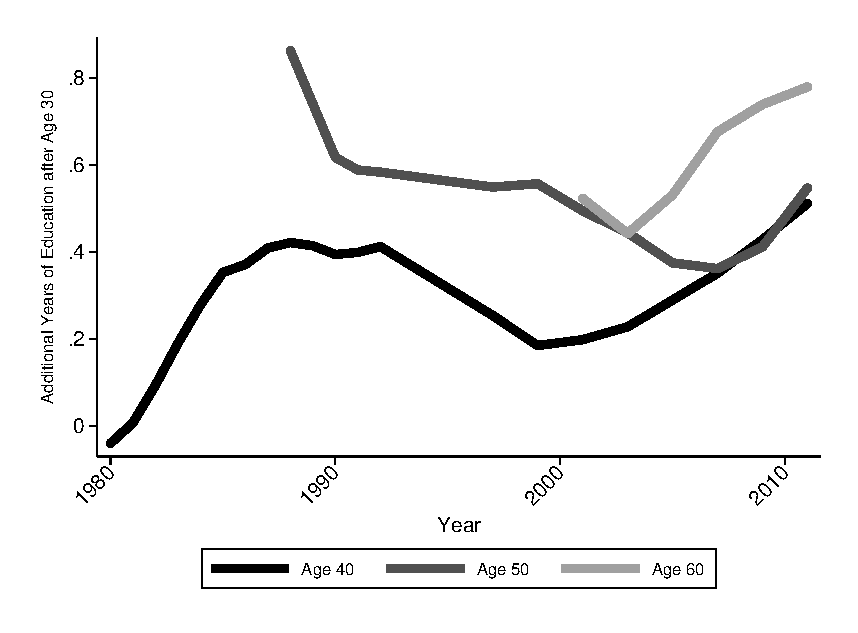
\includegraphics[height=2.5in]{AppOutput/Education/addeducfrom30.eps}
\end{subfigure}%
\begin{subfigure}{.54\textwidth}
  \centering
  \subcaption{ABC-Eligible PSID Educational Attainment by Age}\label{fig:abc-psid-sample}
  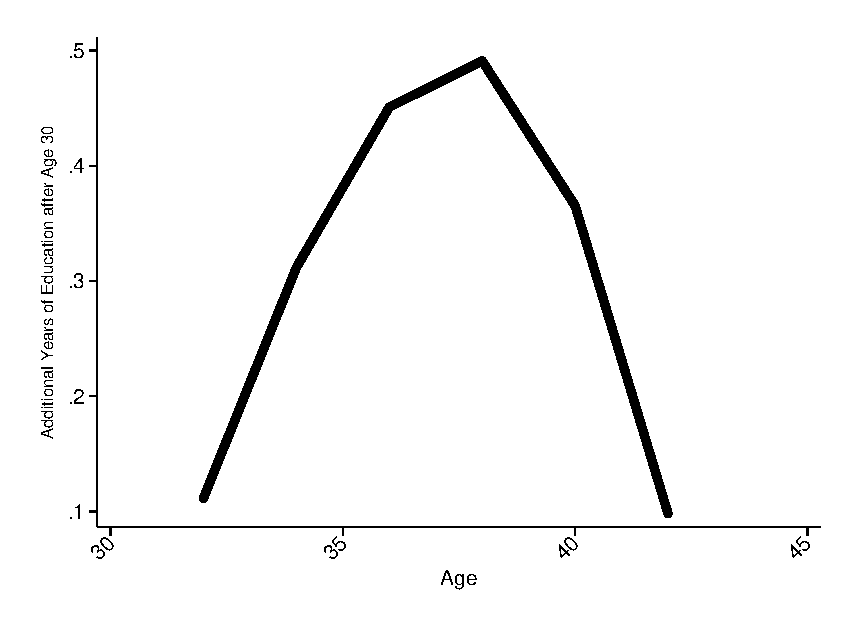
\includegraphics[height=2.5in]{AppOutput/Education/addeducfrom30matched.eps}
\end{subfigure}
\floatfoot{
\scriptsize
Note 1 (left panel): This plot uses data from the Panel Study of Income Dynamics (PSID) to display the mean years of education beyond the education level at age 30, by years. We report this value for ages 40, 50, and 60. The domain of the trends is a function of data availability, i.e. of longitudinal span in the data. Each yearly calculation uses cross-sectional weights to attain nationally representative statistics. \\
Note 2 (right panel): This plot uses a restricted sample of the PSID. We only consider individuals who would have been eligible for ABC and/or CARE following the procedure in \citet{Garcia_Heckman_2014_AbilityCharacter}. We pool all the years and plot the mean years of education beyond the education level at age 30, by age.
}
\end{figure}

\noindent Figure~\ref{fig:psid-yearly-all} displays the average additional years of education at ages 40, 50, and 60. The series have different spans due to restrictions in data availability. Figure~\ref{fig:abc-psid-sample} uses a sample of individuals that would have been eligible to be part of ABC or CARE. Furthermore, we restrict the sample to the 1972--1982 cohort of PSID, to mimic the ABC and CARE samples. To find the eligible sample we follow the same procedure as \citet{Garcia_Heckman_2014_AbilityCharacter}. Broadly, we reconstruct the ABC High-risk Index in the PSID and construct a sample of ``ABC-eligible individuals.'' The data availability is not enough to perform a yearly analysis. We pool all the available years to construct this plot---roughly, 1990 to 2010. Both plots show that individuals, on average, never go a year beyond their education at age 30. We assume that imprecision generated by not observing educational levels beyond age 30 is of second order, and do not project additional educational attainment. \\


\subsection{Treatment Effects on Education}
\noindent To analyze the long-term impact of ABC and CARE on educational attainment,
we examine data on grade retention, special education, and
years/type of schooling through age 30. After age 30,
educational attainment remains essentially
unchanged.%
	\footnote{Our calculation is based on
	the data from the Panel of Study of Income Dynamics (PSID) for a
	population born between 1972 and 1982 (the same age group as that of
	ABC subjects). The data show that on average, the mean years of education attained
	beyond age 30 was less than one year.
	Therefore, any potential concerns regarding uncertainties of our analysis
	by not observing educational levels beyond age 30 is second
	order.}
The benefits of additional schooling, e.g. through
increased income and improved health, is assessed in
subsequent sections. Here we focus on estimating the
differences in schooling costs between the treatment and
control groups. \\

\subsection{Cost of Education}
\noindent We apply the costs described in Table \ref{tab:yearlyedu} to subjects' educational attainment at age 30 to calculate the public and private costs of lifetime educational attainment. Costs up to high school are assumed to be public costs. \\

\begin{table}[H]
\caption{Yearly Individual Education Costs} \label{tab:yearlyedu}
\centering
\begin{adjustbox}{max width=\textwidth}
\begin{threeparttable}
\footnotesize
\begin{tabular}{C{3.5cm} C{1.5cm} C{1.5cm} C{2cm} C{6.5cm}}
\toprule
Schooling level & Ages & Duration (Years) & Yearly Cost &Attainment \& Notes\\ \midrule

K-8 & 6-14 & 8 & \$9,113  & All subjects. Assume dropout before Grade 9 completed up to Grade 8. \\
\\

High School (Not Completed) & 15-16 & 2 &   \$9,113  &  This is from Grade 9 to Grade 10. Assume high school dropout completed up to Grade 10.  \\ \\

High School (Completed) & 15-18 & 4 &   \$9,113  &  This is from Grade 9 to Grade 12. 47:38 (control:treatment) \\ \\

GED (Not Completed) & 18 & .5 &  \$155& GED is considered a one year program. No subjects identified as having starting a GED program without finishing.\\ \\
GED (Completed) & 18 & 1 & \$155 & 1:1 (control:treatment).\\ \\
Community College/Technical Training (Not Completed) &   19 & 1 &  \$7,001 & Assume dropouts drop at the end of the first year. 19:7 (control:treatment) \\ \\
Community College/Technical Training (Completed) & 19-20 & 2 &  \$7,001 & 18:19 (control:treatment)\\ \\
 Any College (Not Completed)   &  19-20 & 1 &  \$11,886 & Assume dropouts drop out at the end of the second year. 7:11 (control:treatment).\\ \\
 Any College (Completed) &  19-22 & 4 & \$11,886 & 6:14 (control:treatment) \\ 
Graduate School (Not Completed) & 23 & 1 &  \$9,704& Assume dropouts drop out at the end of the first year. 3 treated individuals.\\ \\
 Finished Masters &  23-24 & 2 &  \$9,704 & 1 treated individual\\ \\
 Finished PhD & 23-26 & 4 & \$9,704 & 1 treated individual\\ \\
 \midrule
 Grade Retention& NA & 1 &\$9,113 & \\ \\
 Special Ed.& NA & 1 &  \$11,705  & \\ 
 \bottomrule
 \end{tabular}

\centering
\begin{tablenotes}%[para,flushleft]
\scriptsize
\item Sources: \citet{Snyder_Willow_2012_BOOK_NCES}; \citet{Hoenack_Weiler_1975_JHR}; \cite{Dhanidina_Griffith_1975_AEQ}; \cite{Freeman_1974_Occupational-Training_RES}. \\
 Note: This table reports the yearly cost and duration of each type of education, as well as the ages for which we evaluate them.  All amounts are inflated to 2014 USD.
We show the number of subjects who identified themselves as being in each education category (total number of respondents: 101/114). To compute the total cost of education for a subject, we applied these costs additively up to the highest level of educational attainment. Only K-12 education, special  education, and grade retention costs account for deadweight loss. Because it gives costs that are applied across many years, this table does not show their present discounted value.
\end{tablenotes}
\end{threeparttable}
\end{adjustbox}
\end{table}


\subsection{Non-monetary Benefits of Education}

\noindent There are many social and non-monetary benefits of education that our analysis cannot capture. These benefits impact the individual's quality of life, the general well-being of society through positive peer effects as well as fewer costs and negative externalities, and even the well-being of future generations. Documenting them all may be impossible, but we briefly review some major benefits in this section. \cite{Vila_2000_Non-Monetary-Benefits-Education} documents private benefits with external effects, such as health (increases in longevity and better nutrition and preventative care choices). Higher education is also associated with decreased fertility rates linked with improved infant health and lower mortality rates. Moreover, higher education not only improves labor outcomes with respect to employment prospects and salary, but also with regard to how individuals perceive work and leisure, with more education leading to increased satisfaction from leisure. Furthermore, higher education is linked with better savings behavior and higher rates of return on savings. Higher education is also connected with social stability---better education promotes good citizenship and creates communities that are less likely to experience violent social conflict.\footnote{\citet{Lochner_2011_Handbook} or \citet{Lochner_2011_NBER}.} \\

\setcounter{figure}{0}  \renewcommand{\thefigure}{E.\arabic{figure}}
\setcounter{table}{0}   \renewcommand{\thetable}{E.\arabic{table}}
\section{Quantifying the Benefits in Crime Reduction} \label{appendix:crime}

\subsection{Data Description}

\noindent The crime data available in ABC and CARE come from four different sources provided by the program, which we supplement with auxiliary datasets. We summarize the ABC and CARE datasets and auxiliary datasets related to crime below. \\

\subsubsection{ABC and CARE Datasets}
\begin{enumerate}
\item Administrative Youth Arrests Dataset.  This dataset is only available for ABC. This dataset records all arrests up to the age at which the data were obtained (April, 1996), when ABC subjects were about 21 years old. The categories of crimes in this dataset are coarser than the ones that we use in the other datasets: it categorizes crimes into property, violent, drug, and miscellaneous crimes. We assume some equivalences, as shown in Table~\ref{tab:crime_cat}.
\item Administrative Adult Arrests Dataset. Gathered when ABC and CARE subjects were around 34 years old, this dataset includes individual data on arrests, with short descriptions of the associated offenses. This dataset includes some subjects for whom the arrest history is missing. To resolve this, we use a methodology (detailed below) involving the sentences data, which does not have missing values.
\item Administrative Sentences Dataset. Gathered when ABC and CARE subjects were about 34 years old, this dataset includes individual data on sentences, with descriptions of the crimes. It also includes total sentence length (projected and actual) and punishment type (jail, prison, parole).
\item Self-reported Adult Crimes Dataset. A module on crimes was included at the age-21 and age-30 interviews for both ABC and CARE. After matching all datasets, we use the information from the self-reported crimes whenever a particular crime does not appear in the other datasets.
\end{enumerate}

\subsubsection{Auxiliary Datasets}
\begin{enumerate}
\item National Crime Victimization Survey (NCVS). The NCVS is a survey (self-reported) on crime victimization reported on the household level. The NCVS does not cover crimes to businesses, and it might under-report crimes that might not be known to all members of a family, such as rape. It also does not give statistics for murders. The data are available from 1993 to 2013. We use NCVS to estimate the total number of victims per type of crime in the U.S., which is used to construct victims-to-arrests ratios.
\item Uniform Crime Reporting Statistics (UCRS). This dataset contains all crimes that are reported to the police. It contains crimes to households, individuals, and businesses that are captured by most of the law enforcement agencies in the country. We used data from UCRS spanning the years 1996 to 2012. We use UCRS as a complement to NCVS when we estimate the total number of victims per type of crime in the U.S. %We use UCR to construct national arrest-to-sentences and victims-to-arrests ratios for our crime categories.
%\item Bureau of Justice Statistics (BJS): the BJS' Arrest Data Analysis Tool has data on arrests per year per type of crime. This data only includes arrests made by state authorities. There are 133 federal authorities with the jurisdiction to arrest individuals, such as the FBI and Custom and Border Patrol, but this data is not publicly available. As with arrests, there is a distinction between Federal and State sentences given to offenders, depending on whether they were convicted in a state or federal court. We also used the BJS's Offender Sentences tool to acquire data on Federal sentences from 1998 to 2012. It is, however, in more general categories and only includes Violent, Property, Public Order, Drug and Other Offenses.
\item National Judicial Reporting Program (NJRP). We use the NJRP to get data for total number of sentences in the U.S. The data were taken from reports published biennially from 1986 to 2006. We use this dataset to construct arrest-to-sentences ratios for our crime categories.
\item North Carolina Department of Public Safety dataset (NCDPS). This dataset contains information since 1972 on each individual who is convicted of a crime and enters the state prison system or community supervision in North Carolina. The data do not include arrests, or sentences involving jail or unsupervised probation. Because the North Carolina Department of Public Safety was created 3 years ago to consolidate the state's Department of Correction, Department of Juvenile Justice, and Crime Control, among other state agencies, these data were mostly constructed by the other agencies. We use this dataset to fit a prediction model that we use to predict future crimes for ABC and CARE subjects.
\end{enumerate}

\subsubsection{Crime Categories}
\noindent The administrative adult datasets have descriptions of all crimes committed by ABC and CARE subjects. We categorize these crimes to be as comparable as possible to the categories in the other data sources and in the literature on calculating the cost of crime. However, it is inevitable to have some crimes that do not clearly fit into the broad categories. As shown in Table \ref{tab:crime_cat}, the different experimental and auxiliary datasets and the literature use different crime categories. The categorization we present is our effort to make all sources comparable. \\

\begin{table}[H]
\begin{threeparttable}
\scriptsize \caption{Crime Categories} \label{tab:crime_cat}
\begin{tabular}{lllll}
\toprule
{Our Categories}	&	{Youth Data} & {Costs of Crime} & {Nat. Arrests Data} & {Nat. Sentences Data}	\\
\midrule
%				&				& \cite{mccollister2010cost} 	&			&					\\ \hline
{Arson}			&			& Arson					&	Arson			&					\\	
{Assault}			&	Violent			& Assault				&	Total assaults	& Aggravated 		\\		
				&				&						&					& assaults 			\\ 		
{Burglary}		&				& Household burglary	&	Burglary		& Burglary			\\		
{Fraud}			&				& Fraud					&	Fraud,			& Fraud,			\\		
				&				&						&	Forgery,		& Forgery			\\
				&				&						&	Embezzlement	&					\\		
{Larceny}			&	Property	& Larceny/theft			&	Larceny			& Larceny/theft		\\		
{Miscellaneous}	& 	Drug, Misc.	& 					&	Drug abuse		& Drug offenses		\\		
				&				&						&	total			&					\\ 		
{Vehicle Theft}	&				& MV theft	&	MV theft		& MV theft			\\		
{Murder}			&				& Murder				&	Murder,			& Murder,			\\	
				&				&						& 	Non-negligent 	& Manslaughter		\\
				&				&						& 	manslaughter	&   				\\
{Rape}			&				& Rape/sexual assault	&	Forcible rape, 	& Rape 				\\
				&				&						&	Sex offense		&					\\
{Robbery}			&				& Robbery 				&	Robbery			&					\\
{Vandalism}		&				& Vandalism				&	Vandalism		& 				\\	\bottomrule
\end{tabular}
\begin{tablenotes}
\item Note: This table shows the various measures we have for our categories of crimes from each dataset. ``Costs of Crime'' are from \cite{McCollister_etal_2010_DAD}.
\end{tablenotes}
\end{threeparttable}
\end{table}

\subsection{Methodology for Estimating Crime Costs}
\noindent In this section we give a detailed explanation of the steps taken to calculate the total treatment effect on crime and the costs associated with that effect. We first give a more abstract and formal summary of the process, and then discuss the details for each step. \\
%We follow four steps towards constructing our estimates: (i) First, we count the total number of arrests and sentences for each ABC study individual up to age 34; (ii) then we predict, based on the age 34 count of sentences, the number of sentences that the ABC  individuals will have in the future; (iii) next, based on the two previous points, and on the national victims-to-arrests and arrests-to-sentences ratios for the different categories of crimes we use, we estimate the number of victims that might have suffered (observed and unobserved) crimes by ABC study participants; (iv) finally, using the estimated numbers of victims, we impute costs of the crimes based on the literature. We discuss in detail the different costs associated with criminal activity, and the two main approaches to these calculations as categorized by Bottom-Up and Top-Down methodologies. We now give a more formal summary of those four steps. The details are discussed in the rest of this section.

\begin{enumerate}
\item \textit{Count Arrests and Sentences}. We count the total number of sentences for each subject, $i$, and category of crime (robbery, larceny, etc.), $j$, up to age 34,  which we denote by $S_{i,j}^{34}$. We also match the data on adult arrests, juvenile arrests, and self-reported crimes, to construct total number of  arrests for each crime type up to that age, $A_{i,j}^{34}$. For some subjects, the arrest data are missing. In those cases, we impute the missing data by assuming that the national arrests-to-sentences ratio for crime type, $j$, is valid for each subject. Let $\overline{A_j}$ be the national total number of arrests for crime type, $j$, and let $\overline{S_j}$ be the national total number of sentences. Then, we construct $r_j=\frac{\overline{A_j}}{\overline{S_j}}$, and we impute $A_{i,j}^{34}=r_j S_{i,j}^{34}$.

\item \textit{Construct Predictions}. From our external data, we have a dataset to predict lifetime sentences. In that dataset, we use sentences up to age 34 in all types of crime to predict future sentences for that crime type, $\widehat{S_{i,j}^{35-50}}$. This gives an estimate of the lifetime sentences as $\widehat{S_{i,j}}=S_{i,j}^{34}+\widehat{S_{i,j}^{35-50}}$. Given that we do not have an analogous dataset to predict lifetime arrests, we impute the predicted arrests as a linear function of the predicted number of sentences: $\widehat{A_{i,j}^{35-50}}=r_j \widehat{S_{i,j}^{35-50}}$. Then, we calculate $\widehat{A_{i,j}}=A_{i,j}^{34}+\widehat{A_{i,j}^{35-50}}$.

\item \textit{Estimate Number of Victims}. Let the national number of victims of a given type of crime be $\overline{V_j}$. We construct a victimization inflation factor for each crime type: $f_j=\frac{\overline{V_j}}{\overline{A_j}}$. It represents the number of times someone is arrested as a fraction of the number of victims of the crimes. Then, the estimated number of victims of subject, $i$, for crime type, $j$, based on arrests is estimated as $\widehat{V_{i,j}^{A}}=A_{i,j}f_j$. For sentences, we calculate an analogous estimate of victims based on the victimization inflation factor and the arrests-to-sentences ratio: $\widehat{V_{i,j}^{S}}=S_{i,j}f_j r_j$. Both estimates are similar, as we show below. We construct our final estimate of the lifetime victims of subject, $i$, for crime type, $j$, as the average of both estimates to achieve greater precision: $\widehat{V_{i,j}}=\left(\widehat{V_{i,j}^A}+\widehat{V_{i,j}^S}\right)/2$.

\item \textit{Find Total Costs of Crimes}. We use estimates of the cost of crimes for victims from the literature for each crime type $j$, $c_j^V$. We impute the total victim costs of subject, $i$, for crime type, $j$, as $\widehat{C_{i,j}^V}=\widehat{V_{i,j}} c_j^V$. We also calculate different costs from the justice system (including police) associated with the different crime types, but only for the ones that included arrests or sentences (i.e. we do not consider the victimization inflation), as: $C_{i,j}^{JS}=\widehat{A_{i,j}} c_j^{JS}$. Finally, we also construct the total costs of incarceration for crime type, $j$, $\widehat{C_{i,j}^{P}}$ as the total time the subject was imprisoned for that type of crime, $P_{i,j}$, multiplied by the cost of a day in prison $c_P$. All of our cost estimates are discounted to birth.
\end{enumerate}


\subsubsection{Count Arrests and Sentences}
\noindent Unlike previous studies, we use several datasets to construct measures of criminal activity of the ABC or CARE subject. We generate a count of the number of arrests and of the number of sentences by crime category for each ABC and CARE subject. We start by counting sentences, which is trivial, as we have complete information on sentences for all ABC and CARE subjects in one dataset. \\

\noindent Unlike counting sentences, the count of arrests is more involved.\footnote{Throughout this appendix, for all the calculations involving counting arrests, if the arrest was the result of more than one \textit{offense}, we count the number and type of offenses separately, rather than counting all of them as one. An offense is the precise definition for the unit that we work with.} We now describe the procedure we follow to get a count of arrests that is as complete as possible. We begin by matching, based on crime description and date, the arrests from the adult administrative data, the youth administrative data, and the self-reported dataset. It is possible that the adult data are missing youth arrests that were expunged from the criminal records or crimes committed in states other than North Carolina, which were not obtained in the collection of administrative data. Because we observe the arrest dates, we confirm that we are not duplicating any arrests. To align the youth arrests data, which are categorized more broadly, we assume that all violent crimes are assaults (the most common category of violent crime in the sample) and that all property crimes are larcenies (the most common category of property crime). We categorize both drug and miscellaneous crimes in the miscellaneous category, for which we do not compute victim costs. \\
%The original number of arrests in the data was 444. Both the youth administrative data and the self-reported arrests were matched in a case-by case basis with the administrative arrest records, thus making the pre-1995 records much more complete. The number of arrests in the data after the matching and elimination of overlapping arrests is 794.

\noindent The main problem we confront with these data is that there are some individuals who are missing data on arrests in the data collected at age 34. We know this is the case because there are sentences for which we do not observe the corresponding arrests. While this is expected for some crimes, such as speeding or shoplifting, it is not possible for others. This seems to be due to the difficulty in collecting administrative information on arrests. Counting arrests using many data sources eases of reconstructing the adult arrests data. We tackle this challenge by first identifying those individuals who should have arrests, because they have sentences that necessarily imply they were arrested at some point of time. Then we impute the number of arrests for each of those sentences, based on the national arrests-to-sentences ratio. We estimate that 11 individuals (10\% of the ABC sample) have missing arrest data. We note that the final estimates of effects on reduction in crime costs using only sentences (which do not have any missing values) are very similar to the ones using arrests. \\

\noindent The effect of adding the different datasets, as well as the final counts of both arrests and sentences is presented in Figure \ref{fig:datagraph}. Thes the first three pairs of bars present the number of additional crimes included in the data by the addition of the self-reported, juvenile, and sentences datasets. In the case of sentences, we first show the effect of imputing just one arrest per sentence, and only for individuals with missing arrests. Notice that the juvenile data only adds assaults, larcenies, and miscellaneous, as discussed above. The next pair of bars shows the effect of adding more than one arrest per sentence for the individuals with missing data, using the arrests-to-sentences ratios. The effect is significant, adding about 30\% more crimes to the previous estimate. Importantly, some rape arrests are added to the control group in this step, because of one subject who presented a sentence for that crime. Finally, the total number of sentences is far lower than the total number of arrests, even if only the original arrests are counted. We also note in this chart that the volume of the crimes is mostly driven by miscellaneous crimes (which are mostly drug and traffic crimes). As these crimes are counted as victimless in our methodology, their effect on the final estimates is much smaller than what this chart might suggest. \\

\begin{figure}[H]
\caption{Counts of Arrests and Sentences}
\centering \label{fig:datagraph}
{\scalebox{0.8}{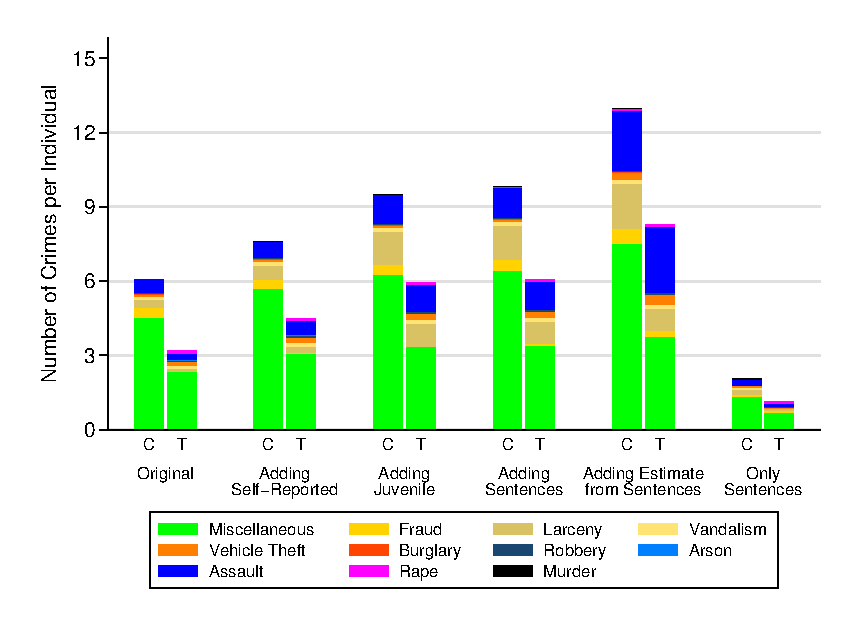
\includegraphics{AppOutput/Crime/counts_misc}}}
\floatfoot{
\footnotesize
\noindent Note: This chart shows the arrests per capita for the control (C) and treatment (T) groups. The first pair of bars shows the original arrests data from the administrative adult dataset. The next pair adds the self-reported crimes that did not match with the original arrests data. The next pair adds data from the administrative juvenile dataset that did not match with the previous datasets. The next pair adds one arrest for every sentence that did not match with the previous datasets and one arrest for every sentence that had arrest data missing. The next pair adds $n$ arrests instead of one for each sentence, where $n$ is calculated using the arrests-to-sentences ratio obtained from auxiliary datasets. The final pair of bars, for reference, is the total number of sentences from the administrative sentences dataset.
}
\end{figure}

\subsubsection{Construct Predictions}

\noindent The data available describe the ABC and CARE subjects' crimes committed up to age 34. However, we believe that the effect of the programs on crime does not stop at that age. To predict the number of crimes that the study participants commit beyond age 34, we use data from the North Carolina Department of Public Safety (NCDPS). Because the crime data are obtained from the same state in which ABC and CARE were implemented, the prediction model is appropriate for the ABC and CARE samples. To the best of our knowledge, no study of the effects of an early childhood education program has ever used microdata to estimate a predictive model for future crimes. The estimations in \cite{Heckman_Moon_etal_2010_RateofReturn} are based on national age ratios (crimes of a certain category committed by older people over crimes of the same category committed by younger people at a specific time), rather than on microdata. However, age ratios only consider the same category of crime as an input to the estimation model and the results can reflect demographic transitions. \\

\noindent It would be ideal to use prediction models estimated from the same cohorts as the ABC and CARE subjects. However, it is not possible to predict crimes committed until older ages because the ABC and CARE subjects are currently about 46 years old. To predict crimes at older ages, it is necessary to use earlier cohorts. The data are available from 1972 (44 years ago as of 2016), and thus they do not contain a complete criminal history for any cohort of individuals. 
%Given that, we have to choose specific cohorts for the estimations, such that they are old enough to cover the ages we need to predict, and young enough to have their entire crime life covered in the dataset, in the same way as the entire crime life of ABC individuals in covered in our data. In particular,
We assume that few crimes are committed after the age of 50. \\
%, and that crime life does not start until age 16.
 We separately estimate predictions from ages 35-40, 40-45, and 45-50. We have plentiful observations to estimate crimes in all the age ranges. %\footnote{As an example, to predict crimes at ages 45-50 we need individuals aged 50+. To have enough birth year cohorts, we consider individuals aged 50-59 in 2015. The oldest of these individuals were aged 16 in 1972, so we can reasonably expect them to having committed few crimes before that year. Finding observations for crime predictions at earlier ages is even easier.}
%Age 5 in 2015-->Age 12 in 1972.            Age 50 in 2015-->Age 16 in 1972.
%Age 55 in 2015-->Age 12 in 1972.            Age 59 in 2015-->Age 16 in 1972.
We calculate our predictions using a five-step procedure: \\
\begin{enumerate}
\item Find individuals that are at least 40 years old as of 2016 in the NCDPS dataset.
\item Regress the number of crimes of each type at ages 35--40 on those at ages 16--34.
\item Use the estimated prediction model for ABC individuals, attributing those crimes to age 40 for discounting purposes.
\item Repeat the three previous steps for ages 40--45 and 45--50. %50-55?
\item For individuals with no criminal histories before age 34, assume that they commit no crimes after 34.
\end{enumerate}

\noindent We perform the previous process separately for males and females. We use linear predictions, but replace negative predicted values of crime by zero. Table~\ref{tab:reg1f} through Table~\ref{tab:reg3m} show the estimated models. As expected, generally the most important prediction factor for a crime is the number of occurrences of the same crime type in a previous period. The coefficients in some cases are substantial, which implies that considering predicted crimes is an important part of an assessment of the crime benefits of the program. \\
%include more tables if ages 55 are covered, not just 50
\begin{sidewaystable}[H]
\caption{NCDPS Regressions of Ages 35--40 on Ages 16--35, Females} \label{tab:reg1f}
\begin{adjustbox}{max width=\textwidth}
\begin{threeparttable}
\begin{tabular}{lccccccccccc}
\toprule \noalign{\smallskip} & Miscellaneous & Fraud & Larceny & Vandalism & Auto Theft & Burglary & Robbery & Arson & Assault & Rape & Murder\\
\noalign{\smallskip}\midrule \noalign{\smallskip}Miscellaneous & 0.103 & -0.029 & 0.009 & 0.001 & 0.001 & 0.001 & 0.000 & -0.000 & 0.002 & -0.000 & -0.001\\
 & \begin{footnotesize}(27.71)**\end{footnotesize} & \begin{footnotesize}(5.90)**\end{footnotesize} & \begin{footnotesize}(6.00)**\end{footnotesize} & \begin{footnotesize}(3.88)**\end{footnotesize} & \begin{footnotesize}(5.18)**\end{footnotesize} & \begin{footnotesize}(2.25)*\end{footnotesize} & \begin{footnotesize}(1.91)\end{footnotesize} & \begin{footnotesize}(0.62)\end{footnotesize} & \begin{footnotesize}(3.16)**\end{footnotesize} & \begin{footnotesize}(1.27)\end{footnotesize} & \begin{footnotesize}(2.85)**\end{footnotesize}\\
\noalign{\smallskip}Fraud & -0.047 & 0.104 & 0.003 & -0.000 & 0.000 & 0.000 & 0.000 & 0.000 & -0.001 & -0.000 & -0.000\\
 & \begin{footnotesize}(21.71)**\end{footnotesize} & \begin{footnotesize}(36.61)**\end{footnotesize} & \begin{footnotesize}(3.81)**\end{footnotesize} & \begin{footnotesize}(2.31)*\end{footnotesize} & \begin{footnotesize}(0.60)\end{footnotesize} & \begin{footnotesize}(2.02)*\end{footnotesize} & \begin{footnotesize}(0.02)\end{footnotesize} & \begin{footnotesize}(1.76)\end{footnotesize} & \begin{footnotesize}(1.48)\end{footnotesize} & \begin{footnotesize}(0.75)\end{footnotesize} & \begin{footnotesize}(1.72)\end{footnotesize}\\
\noalign{\smallskip}Larceny & 0.034 & 0.002 & 0.105 & 0.001 & 0.002 & 0.002 & 0.001 & 0.000 & 0.004 & 0.000 & -0.000\\
 & \begin{footnotesize}(8.16)**\end{footnotesize} & \begin{footnotesize}(0.33)\end{footnotesize} & \begin{footnotesize}(62.36)**\end{footnotesize} & \begin{footnotesize}(2.37)*\end{footnotesize} & \begin{footnotesize}(10.35)**\end{footnotesize} & \begin{footnotesize}(7.80)**\end{footnotesize} & \begin{footnotesize}(5.97)**\end{footnotesize} & \begin{footnotesize}(2.99)**\end{footnotesize} & \begin{footnotesize}(5.65)**\end{footnotesize} & \begin{footnotesize}(1.30)\end{footnotesize} & \begin{footnotesize}(1.67)\end{footnotesize}\\
\noalign{\smallskip}Vandal & 0.000 & -0.036 & -0.024 & 0.012 & 0.004 & 0.007 & 0.005 & 0.003 & 0.043 & 0.000 & -0.000\\
 & \begin{footnotesize}(0.01)\end{footnotesize} & \begin{footnotesize}(1.10)\end{footnotesize} & \begin{footnotesize}(2.43)*\end{footnotesize} & \begin{footnotesize}(6.40)**\end{footnotesize} & \begin{footnotesize}(2.86)**\end{footnotesize} & \begin{footnotesize}(3.87)**\end{footnotesize} & \begin{footnotesize}(3.34)**\end{footnotesize} & \begin{footnotesize}(3.40)**\end{footnotesize} & \begin{footnotesize}(9.27)**\end{footnotesize} & \begin{footnotesize}(0.79)\end{footnotesize} & \begin{footnotesize}(0.23)\end{footnotesize}\\
\noalign{\smallskip}Auto Theft & 0.059 & -0.026 & 0.055 & 0.004 & 0.012 & 0.007 & 0.005 & -0.002 & -0.014 & -0.000 & 0.002\\
 & \begin{footnotesize}(1.55)\end{footnotesize} & \begin{footnotesize}(0.52)\end{footnotesize} & \begin{footnotesize}(3.57)**\end{footnotesize} & \begin{footnotesize}(1.28)\end{footnotesize} & \begin{footnotesize}(5.94)**\end{footnotesize} & \begin{footnotesize}(2.48)*\end{footnotesize} & \begin{footnotesize}(2.52)*\end{footnotesize} & \begin{footnotesize}(1.30)\end{footnotesize} & \begin{footnotesize}(2.02)*\end{footnotesize} & \begin{footnotesize}(0.23)\end{footnotesize} & \begin{footnotesize}(1.02)\end{footnotesize}\\
\noalign{\smallskip}Burglary & 0.049 & -0.031 & 0.011 & 0.002 & 0.006 & 0.044 & 0.000 & -0.001 & -0.003 & -0.000 & -0.001\\
 & \begin{footnotesize}(1.77)\end{footnotesize} & \begin{footnotesize}(0.86)\end{footnotesize} & \begin{footnotesize}(1.01)\end{footnotesize} & \begin{footnotesize}(0.95)\end{footnotesize} & \begin{footnotesize}(3.86)**\end{footnotesize} & \begin{footnotesize}(22.56)**\end{footnotesize} & \begin{footnotesize}(0.20)\end{footnotesize} & \begin{footnotesize}(1.26)\end{footnotesize} & \begin{footnotesize}(0.55)\end{footnotesize} & \begin{footnotesize}(0.25)\end{footnotesize} & \begin{footnotesize}(0.34)\end{footnotesize}\\
\noalign{\smallskip}Robbery & 0.030 & 0.054 & 0.040 & 0.002 & 0.005 & -0.001 & 0.028 & 0.002 & -0.000 & -0.000 & 0.002\\
 & \begin{footnotesize}(1.05)\end{footnotesize} & \begin{footnotesize}(1.46)\end{footnotesize} & \begin{footnotesize}(3.51)**\end{footnotesize} & \begin{footnotesize}(1.03)\end{footnotesize} & \begin{footnotesize}(3.43)**\end{footnotesize} & \begin{footnotesize}(0.28)\end{footnotesize} & \begin{footnotesize}(17.69)**\end{footnotesize} & \begin{footnotesize}(2.22)*\end{footnotesize} & \begin{footnotesize}(0.07)\end{footnotesize} & \begin{footnotesize}(0.29)\end{footnotesize} & \begin{footnotesize}(1.50)\end{footnotesize}\\
\noalign{\smallskip}Arson & 0.070 & -0.087 & -0.035 & 0.008 & 0.011 & 0.006 & 0.025 & 0.010 & 0.017 & -0.000 & 0.005\\
 & \begin{footnotesize}(1.29)\end{footnotesize} & \begin{footnotesize}(1.22)\end{footnotesize} & \begin{footnotesize}(1.61)\end{footnotesize} & \begin{footnotesize}(1.98)*\end{footnotesize} & \begin{footnotesize}(3.98)**\end{footnotesize} & \begin{footnotesize}(1.62)\end{footnotesize} & \begin{footnotesize}(8.19)**\end{footnotesize} & \begin{footnotesize}(4.95)**\end{footnotesize} & \begin{footnotesize}(1.67)\end{footnotesize} & \begin{footnotesize}(0.19)\end{footnotesize} & \begin{footnotesize}(1.60)\end{footnotesize}\\
\noalign{\smallskip}Assault & 0.064 & -0.060 & 0.007 & 0.007 & 0.001 & 0.002 & -0.000 & 0.002 & 0.048 & -0.000 & 0.000\\
 & \begin{footnotesize}(5.74)**\end{footnotesize} & \begin{footnotesize}(4.11)**\end{footnotesize} & \begin{footnotesize}(1.63)\end{footnotesize} & \begin{footnotesize}(7.82)**\end{footnotesize} & \begin{footnotesize}(1.83)\end{footnotesize} & \begin{footnotesize}(1.93)\end{footnotesize} & \begin{footnotesize}(0.14)\end{footnotesize} & \begin{footnotesize}(4.52)**\end{footnotesize} & \begin{footnotesize}(22.78)**\end{footnotesize} & \begin{footnotesize}(0.36)\end{footnotesize} & \begin{footnotesize}(0.34)\end{footnotesize}\\
\noalign{\smallskip}Rape & -0.015 & -0.131 & -0.003 & -0.003 & -0.003 & -0.004 & -0.006 & -0.001 & 0.001 & -0.000 & -0.002\\
 & \begin{footnotesize}(0.15)\end{footnotesize} & \begin{footnotesize}(0.98)\end{footnotesize} & \begin{footnotesize}(0.08)\end{footnotesize} & \begin{footnotesize}(0.42)\end{footnotesize} & \begin{footnotesize}(0.49)\end{footnotesize} & \begin{footnotesize}(0.55)\end{footnotesize} & \begin{footnotesize}(0.99)\end{footnotesize} & \begin{footnotesize}(0.24)\end{footnotesize} & \begin{footnotesize}(0.08)\end{footnotesize} & \begin{footnotesize}(0.06)\end{footnotesize} & \begin{footnotesize}(0.33)\end{footnotesize}\\
\noalign{\smallskip}Murder & 0.006 & -0.166 & -0.008 & 0.003 & -0.002 & -0.002 & -0.002 & 0.003 & 0.001 & -0.000 & -0.001\\
 & \begin{footnotesize}(0.16)\end{footnotesize} & \begin{footnotesize}(3.44)**\end{footnotesize} & \begin{footnotesize}(0.54)\end{footnotesize} & \begin{footnotesize}(1.19)\end{footnotesize} & \begin{footnotesize}(0.94)\end{footnotesize} & \begin{footnotesize}(0.75)\end{footnotesize} & \begin{footnotesize}(1.22)\end{footnotesize} & \begin{footnotesize}(2.24)*\end{footnotesize} & \begin{footnotesize}(0.12)\end{footnotesize} & \begin{footnotesize}(0.34)\end{footnotesize} & \begin{footnotesize}(0.37)\end{footnotesize}\\
\noalign{\smallskip}constant & 0.069 & 0.267 & 0.041 & 0.004 & 0.001 & 0.001 & 0.001 & 0.001 & 0.023 & 0.000 & 0.004\\
 & \begin{footnotesize}(13.39)**\end{footnotesize} & \begin{footnotesize}(39.01)**\end{footnotesize} & \begin{footnotesize}(19.54)**\end{footnotesize} & \begin{footnotesize}(10.27)**\end{footnotesize} & \begin{footnotesize}(2.76)**\end{footnotesize} & \begin{footnotesize}(3.17)**\end{footnotesize} & \begin{footnotesize}(4.80)**\end{footnotesize} & \begin{footnotesize}(3.52)**\end{footnotesize} & \begin{footnotesize}(23.81)**\end{footnotesize} & \begin{footnotesize}(3.38)**\end{footnotesize} & \begin{footnotesize}(12.90)**\end{footnotesize}\\
\noalign{\smallskip}$R^2$ & 0.02 & 0.02 & 0.07 & 0.00 & 0.01 & 0.01 & 0.01 & 0.00 & 0.01 & 0.00 & 0.00\\
$N$ & 63,515 & 63,515 & 63,515 & 63,515 & 63,515 & 63,515 & 63,515 & 63,515 & 63,515 & 63,515 & 63,515\\
\noalign{\smallskip}\bottomrule\end{tabular}

\begin{tablenotes}
\item Note: This table shows how the crimes at ages 35--40 (in the columns) are predicted by crimes at ages 16--35 (in the rows). The estimations are predicted using the North Carolina Department of Public Safety dataset, which contains information on all individuals that have ever been sentenced in North Carolina. We use linear regressions in all cases. The sample for this model is limited to individuals who are at least 40 years old. *~$p<0.05$; **~$p<0.01$.
\end{tablenotes}
\end{threeparttable}
\end{adjustbox}
\end{sidewaystable}


\begin{sidewaystable}[H]
\caption{NCDPS Regressions of Ages 35--40 on Ages 16--35, Males} \label{tab:reg1m}
\begin{adjustbox}{max width=\textwidth}
\begin{threeparttable}
\begin{tabular}{lccccccccccc}
\toprule \noalign{\smallskip} & Miscellaneous & Fraud & Larceny & Vandalism & Auto Theft & Burglary & Robbery & Arson & Assault & Rape & Murder\\
\noalign{\smallskip}\midrule \noalign{\smallskip}Miscellaneous & 0.095 & -0.002 & 0.004 & 0.000 & 0.001 & 0.001 & 0.000 & -0.000 & 0.005 & -0.001 & -0.001\\
 & \begin{footnotesize}(73.29)**\end{footnotesize} & \begin{footnotesize}(2.13)*\end{footnotesize} & \begin{footnotesize}(8.97)**\end{footnotesize} & \begin{footnotesize}(2.71)**\end{footnotesize} & \begin{footnotesize}(6.47)**\end{footnotesize} & \begin{footnotesize}(5.87)**\end{footnotesize} & \begin{footnotesize}(1.50)\end{footnotesize} & \begin{footnotesize}(0.12)\end{footnotesize} & \begin{footnotesize}(14.73)**\end{footnotesize} & \begin{footnotesize}(3.28)**\end{footnotesize} & \begin{footnotesize}(5.83)**\end{footnotesize}\\
\noalign{\smallskip}Fraud & -0.025 & 0.107 & 0.007 & 0.000 & 0.001 & 0.002 & 0.001 & -0.000 & -0.000 & -0.000 & -0.000\\
 & \begin{footnotesize}(13.76)**\end{footnotesize} & \begin{footnotesize}(67.23)**\end{footnotesize} & \begin{footnotesize}(11.68)**\end{footnotesize} & \begin{footnotesize}(0.47)\end{footnotesize} & \begin{footnotesize}(3.44)**\end{footnotesize} & \begin{footnotesize}(5.27)**\end{footnotesize} & \begin{footnotesize}(2.53)*\end{footnotesize} & \begin{footnotesize}(0.61)\end{footnotesize} & \begin{footnotesize}(0.34)\end{footnotesize} & \begin{footnotesize}(0.35)\end{footnotesize} & \begin{footnotesize}(1.96)*\end{footnotesize}\\
\noalign{\smallskip}Larceny & 0.041 & 0.012 & 0.092 & 0.001 & 0.005 & 0.010 & 0.004 & 0.000 & 0.009 & -0.000 & -0.000\\
 & \begin{footnotesize}(14.34)**\end{footnotesize} & \begin{footnotesize}(4.83)**\end{footnotesize} & \begin{footnotesize}(97.06)**\end{footnotesize} & \begin{footnotesize}(5.13)**\end{footnotesize} & \begin{footnotesize}(14.85)**\end{footnotesize} & \begin{footnotesize}(19.72)**\end{footnotesize} & \begin{footnotesize}(12.30)**\end{footnotesize} & \begin{footnotesize}(1.79)\end{footnotesize} & \begin{footnotesize}(11.37)**\end{footnotesize} & \begin{footnotesize}(0.46)\end{footnotesize} & \begin{footnotesize}(0.59)\end{footnotesize}\\
\noalign{\smallskip}Vandal & 0.041 & -0.017 & -0.007 & 0.019 & 0.002 & 0.002 & 0.002 & 0.002 & 0.029 & 0.001 & 0.000\\
 & \begin{footnotesize}(4.51)**\end{footnotesize} & \begin{footnotesize}(2.13)*\end{footnotesize} & \begin{footnotesize}(2.22)*\end{footnotesize} & \begin{footnotesize}(23.49)**\end{footnotesize} & \begin{footnotesize}(1.96)\end{footnotesize} & \begin{footnotesize}(1.06)\end{footnotesize} & \begin{footnotesize}(1.76)\end{footnotesize} & \begin{footnotesize}(5.41)**\end{footnotesize} & \begin{footnotesize}(11.26)**\end{footnotesize} & \begin{footnotesize}(1.06)\end{footnotesize} & \begin{footnotesize}(0.62)\end{footnotesize}\\
\noalign{\smallskip}Auto Theft & 0.015 & 0.014 & 0.005 & 0.002 & 0.043 & 0.013 & 0.000 & 0.000 & 0.008 & 0.001 & 0.001\\
 & \begin{footnotesize}(1.58)\end{footnotesize} & \begin{footnotesize}(1.70)\end{footnotesize} & \begin{footnotesize}(1.48)\end{footnotesize} & \begin{footnotesize}(1.86)\end{footnotesize} & \begin{footnotesize}(39.51)**\end{footnotesize} & \begin{footnotesize}(7.87)**\end{footnotesize} & \begin{footnotesize}(0.14)\end{footnotesize} & \begin{footnotesize}(0.13)\end{footnotesize} & \begin{footnotesize}(3.12)**\end{footnotesize} & \begin{footnotesize}(1.28)\end{footnotesize} & \begin{footnotesize}(1.18)\end{footnotesize}\\
\noalign{\smallskip}Burglary & 0.005 & 0.011 & 0.010 & 0.002 & 0.004 & 0.040 & 0.003 & -0.000 & 0.003 & 0.001 & -0.000\\
 & \begin{footnotesize}(1.26)\end{footnotesize} & \begin{footnotesize}(3.06)**\end{footnotesize} & \begin{footnotesize}(6.86)**\end{footnotesize} & \begin{footnotesize}(4.33)**\end{footnotesize} & \begin{footnotesize}(9.17)**\end{footnotesize} & \begin{footnotesize}(52.89)**\end{footnotesize} & \begin{footnotesize}(6.55)**\end{footnotesize} & \begin{footnotesize}(0.30)\end{footnotesize} & \begin{footnotesize}(2.34)*\end{footnotesize} & \begin{footnotesize}(2.37)*\end{footnotesize} & \begin{footnotesize}(0.73)\end{footnotesize}\\
\noalign{\smallskip}Robbery & -0.032 & 0.000 & 0.011 & 0.000 & 0.003 & 0.006 & 0.019 & -0.000 & -0.000 & 0.000 & 0.001\\
 & \begin{footnotesize}(5.06)**\end{footnotesize} & \begin{footnotesize}(0.01)\end{footnotesize} & \begin{footnotesize}(5.42)**\end{footnotesize} & \begin{footnotesize}(0.67)\end{footnotesize} & \begin{footnotesize}(4.61)**\end{footnotesize} & \begin{footnotesize}(5.67)**\end{footnotesize} & \begin{footnotesize}(26.50)**\end{footnotesize} & \begin{footnotesize}(1.00)\end{footnotesize} & \begin{footnotesize}(0.21)\end{footnotesize} & \begin{footnotesize}(0.00)\end{footnotesize} & \begin{footnotesize}(1.68)\end{footnotesize}\\
\noalign{\smallskip}Arson & 0.008 & -0.023 & -0.010 & 0.012 & -0.004 & 0.008 & 0.004 & 0.007 & 0.031 & -0.001 & 0.001\\
 & \begin{footnotesize}(0.26)\end{footnotesize} & \begin{footnotesize}(0.82)\end{footnotesize} & \begin{footnotesize}(0.95)\end{footnotesize} & \begin{footnotesize}(4.40)**\end{footnotesize} & \begin{footnotesize}(0.98)\end{footnotesize} & \begin{footnotesize}(1.44)\end{footnotesize} & \begin{footnotesize}(1.22)\end{footnotesize} & \begin{footnotesize}(6.73)**\end{footnotesize} & \begin{footnotesize}(3.49)**\end{footnotesize} & \begin{footnotesize}(0.21)\end{footnotesize} & \begin{footnotesize}(0.39)\end{footnotesize}\\
\noalign{\smallskip}Assault & 0.041 & -0.010 & -0.000 & 0.005 & -0.001 & 0.000 & 0.002 & 0.000 & 0.051 & 0.001 & 0.001\\
 & \begin{footnotesize}(11.14)**\end{footnotesize} & \begin{footnotesize}(3.18)**\end{footnotesize} & \begin{footnotesize}(0.09)\end{footnotesize} & \begin{footnotesize}(15.94)**\end{footnotesize} & \begin{footnotesize}(1.60)\end{footnotesize} & \begin{footnotesize}(0.12)\end{footnotesize} & \begin{footnotesize}(4.47)**\end{footnotesize} & \begin{footnotesize}(2.56)*\end{footnotesize} & \begin{footnotesize}(49.57)**\end{footnotesize} & \begin{footnotesize}(3.43)**\end{footnotesize} & \begin{footnotesize}(3.29)**\end{footnotesize}\\
\noalign{\smallskip}Rape & -0.003 & -0.016 & -0.010 & -0.002 & -0.002 & -0.006 & -0.002 & -0.000 & -0.004 & 0.011 & -0.001\\
 & \begin{footnotesize}(0.33)\end{footnotesize} & \begin{footnotesize}(1.77)\end{footnotesize} & \begin{footnotesize}(2.86)**\end{footnotesize} & \begin{footnotesize}(2.32)*\end{footnotesize} & \begin{footnotesize}(1.72)\end{footnotesize} & \begin{footnotesize}(3.42)**\end{footnotesize} & \begin{footnotesize}(1.66)\end{footnotesize} & \begin{footnotesize}(0.54)\end{footnotesize} & \begin{footnotesize}(1.21)\end{footnotesize} & \begin{footnotesize}(8.61)**\end{footnotesize} & \begin{footnotesize}(1.69)\end{footnotesize}\\
\noalign{\smallskip}Murder & -0.086 & -0.053 & -0.025 & -0.002 & -0.004 & -0.011 & -0.001 & -0.001 & -0.007 & -0.003 & 0.003\\
 & \begin{footnotesize}(6.33)**\end{footnotesize} & \begin{footnotesize}(4.45)**\end{footnotesize} & \begin{footnotesize}(5.51)**\end{footnotesize} & \begin{footnotesize}(1.71)\end{footnotesize} & \begin{footnotesize}(2.54)*\end{footnotesize} & \begin{footnotesize}(4.31)**\end{footnotesize} & \begin{footnotesize}(0.87)\end{footnotesize} & \begin{footnotesize}(1.53)\end{footnotesize} & \begin{footnotesize}(1.79)\end{footnotesize} & \begin{footnotesize}(1.56)\end{footnotesize} & \begin{footnotesize}(3.35)**\end{footnotesize}\\
\noalign{\smallskip}constant & 0.213 & 0.124 & 0.031 & 0.005 & 0.004 & 0.011 & 0.006 & 0.001 & 0.048 & 0.009 & 0.006\\
 & \begin{footnotesize}(69.25)**\end{footnotesize} & \begin{footnotesize}(45.55)**\end{footnotesize} & \begin{footnotesize}(29.74)**\end{footnotesize} & \begin{footnotesize}(18.57)**\end{footnotesize} & \begin{footnotesize}(10.95)**\end{footnotesize} & \begin{footnotesize}(19.97)**\end{footnotesize} & \begin{footnotesize}(17.78)**\end{footnotesize} & \begin{footnotesize}(9.22)**\end{footnotesize} & \begin{footnotesize}(55.54)**\end{footnotesize} & \begin{footnotesize}(24.70)**\end{footnotesize} & \begin{footnotesize}(27.76)**\end{footnotesize}\\
\noalign{\smallskip}$R^2$ & 0.03 & 0.02 & 0.05 & 0.01 & 0.01 & 0.02 & 0.01 & 0.00 & 0.02 & 0.00 & 0.00\\
$N$ & 230,706 & 230,706 & 230,706 & 230,706 & 230,706 & 230,706 & 230,706 & 230,706 & 230,706 & 230,706 & 230,706\\
\noalign{\smallskip}\bottomrule \end{tabular}

\begin{tablenotes}
\item Note: This table shows how the crimes at ages 35--40 (in the columns) are predicted by crimes at ages 16--35 (in the rows). The estimations are predicted using the North Carolina Department of Public Safety dataset, which contains information on all individuals that have ever been sentenced in North Carolina. We use linear regressions in all cases. The sample for this model is limited to individuals who are at least 40 years old. *~$p<0.05$; **~$p<0.01$.
\end{tablenotes}
\end{threeparttable}
\end{adjustbox}
\end{sidewaystable}

\begin{sidewaystable}[H]
\caption{NCDPS Regressions of Ages 40--45 on Ages 16--35, Females} \label{tab:reg2f}
\begin{adjustbox}{max width=\textwidth}
\begin{threeparttable}
\begin{tabular}{lccccccccccc}
\hline\hline \noalign{\smallskip} & Miscellaneous & Fraud & Larceny & Vandalism & Auto Theft & Burglary & Robbery & Arson & Assault & Rape & Murder\\
\noalign{\smallskip}\hline \noalign{\smallskip}Miscellaneous & 0.020 & -0.006 & -0.001 & 0.000 & 0.000 & 0.000 & -0.000 & 0.000 & 0.001 & 0.000 & -0.001\\
 & \begin{footnotesize}(4.33)**\end{footnotesize} & \begin{footnotesize}(5.18)**\end{footnotesize} & \begin{footnotesize}(0.85)\end{footnotesize} & \begin{footnotesize}(0.78)\end{footnotesize} & \begin{footnotesize}(0.46)\end{footnotesize} & \begin{footnotesize}(1.29)\end{footnotesize} & \begin{footnotesize}(0.11)\end{footnotesize} & \begin{footnotesize}(0.84)\end{footnotesize} & \begin{footnotesize}(0.64)\end{footnotesize} & \begin{footnotesize}(3.66)**\end{footnotesize} & \begin{footnotesize}(2.65)**\end{footnotesize}\\
\noalign{\smallskip}Fraud & 0.046 & 0.003 & 0.002 & 0.000 & 0.001 & -0.000 & 0.000 & -0.000 & -0.000 & 0.000 & -0.000\\
 & \begin{footnotesize}(19.30)**\end{footnotesize} & \begin{footnotesize}(4.41)**\end{footnotesize} & \begin{footnotesize}(2.86)**\end{footnotesize} & \begin{footnotesize}(1.50)\end{footnotesize} & \begin{footnotesize}(4.86)**\end{footnotesize} & \begin{footnotesize}(0.56)\end{footnotesize} & \begin{footnotesize}(1.62)\end{footnotesize} & \begin{footnotesize}(0.62)\end{footnotesize} & \begin{footnotesize}(1.13)\end{footnotesize} & \begin{footnotesize}(2.50)*\end{footnotesize} & \begin{footnotesize}(0.44)\end{footnotesize}\\
\noalign{\smallskip}Larceny & 0.025 & -0.002 & 0.070 & 0.000 & 0.001 & 0.002 & 0.000 & -0.000 & 0.004 & -0.000 & -0.000\\
 & \begin{footnotesize}(5.12)**\end{footnotesize} & \begin{footnotesize}(1.54)\end{footnotesize} & \begin{footnotesize}(41.35)**\end{footnotesize} & \begin{footnotesize}(0.06)\end{footnotesize} & \begin{footnotesize}(3.61)**\end{footnotesize} & \begin{footnotesize}(6.68)**\end{footnotesize} & \begin{footnotesize}(0.75)\end{footnotesize} & \begin{footnotesize}(1.27)\end{footnotesize} & \begin{footnotesize}(5.02)**\end{footnotesize} & \begin{footnotesize}(0.45)\end{footnotesize} & \begin{footnotesize}(0.45)\end{footnotesize}\\
\noalign{\smallskip}Vandal & -0.016 & -0.009 & -0.018 & 0.002 & -0.001 & 0.005 & 0.001 & 0.003 & 0.019 & -0.000 & -0.001\\
 & \begin{footnotesize}(0.52)\end{footnotesize} & \begin{footnotesize}(1.22)\end{footnotesize} & \begin{footnotesize}(1.71)\end{footnotesize} & \begin{footnotesize}(1.02)\end{footnotesize} & \begin{footnotesize}(0.58)\end{footnotesize} & \begin{footnotesize}(2.66)**\end{footnotesize} & \begin{footnotesize}(0.38)\end{footnotesize} & \begin{footnotesize}(3.06)**\end{footnotesize} & \begin{footnotesize}(3.54)**\end{footnotesize} & \begin{footnotesize}(0.71)\end{footnotesize} & \begin{footnotesize}(0.49)\end{footnotesize}\\
\noalign{\smallskip}Auto Theft & 0.012 & -0.011 & 0.010 & 0.004 & 0.012 & 0.013 & -0.001 & -0.001 & -0.017 & 0.007 & 0.001\\
 & \begin{footnotesize}(0.25)\end{footnotesize} & \begin{footnotesize}(0.87)\end{footnotesize} & \begin{footnotesize}(0.56)\end{footnotesize} & \begin{footnotesize}(0.95)\end{footnotesize} & \begin{footnotesize}(4.90)**\end{footnotesize} & \begin{footnotesize}(4.70)**\end{footnotesize} & \begin{footnotesize}(0.36)\end{footnotesize} & \begin{footnotesize}(0.49)\end{footnotesize} & \begin{footnotesize}(1.98)*\end{footnotesize} & \begin{footnotesize}(11.24)**\end{footnotesize} & \begin{footnotesize}(0.41)\end{footnotesize}\\
\noalign{\smallskip}Burglary & -0.034 & 0.019 & 0.007 & -0.003 & 0.005 & 0.007 & 0.004 & 0.000 & -0.004 & 0.001 & -0.001\\
 & \begin{footnotesize}(1.05)\end{footnotesize} & \begin{footnotesize}(2.33)*\end{footnotesize} & \begin{footnotesize}(0.64)\end{footnotesize} & \begin{footnotesize}(1.05)\end{footnotesize} & \begin{footnotesize}(3.12)**\end{footnotesize} & \begin{footnotesize}(3.66)**\end{footnotesize} & \begin{footnotesize}(2.09)*\end{footnotesize} & \begin{footnotesize}(0.22)\end{footnotesize} & \begin{footnotesize}(0.67)\end{footnotesize} & \begin{footnotesize}(2.93)**\end{footnotesize} & \begin{footnotesize}(0.55)\end{footnotesize}\\
\noalign{\smallskip}Robbery & 0.027 & 0.004 & 0.021 & 0.004 & 0.002 & 0.007 & 0.015 & -0.001 & 0.018 & -0.000 & -0.001\\
 & \begin{footnotesize}(0.81)\end{footnotesize} & \begin{footnotesize}(0.47)\end{footnotesize} & \begin{footnotesize}(1.81)\end{footnotesize} & \begin{footnotesize}(1.52)\end{footnotesize} & \begin{footnotesize}(1.21)\end{footnotesize} & \begin{footnotesize}(3.98)**\end{footnotesize} & \begin{footnotesize}(6.93)**\end{footnotesize} & \begin{footnotesize}(0.58)\end{footnotesize} & \begin{footnotesize}(3.19)**\end{footnotesize} & \begin{footnotesize}(0.67)\end{footnotesize} & \begin{footnotesize}(0.82)\end{footnotesize}\\
\noalign{\smallskip}Arson & -0.042 & -0.016 & -0.025 & 0.013 & -0.001 & -0.002 & 0.001 & -0.001 & 0.001 & -0.000 & -0.002\\
 & \begin{footnotesize}(0.65)\end{footnotesize} & \begin{footnotesize}(0.97)\end{footnotesize} & \begin{footnotesize}(1.09)\end{footnotesize} & \begin{footnotesize}(2.63)**\end{footnotesize} & \begin{footnotesize}(0.46)\end{footnotesize} & \begin{footnotesize}(0.57)\end{footnotesize} & \begin{footnotesize}(0.31)\end{footnotesize} & \begin{footnotesize}(0.44)\end{footnotesize} & \begin{footnotesize}(0.12)\end{footnotesize} & \begin{footnotesize}(0.06)\end{footnotesize} & \begin{footnotesize}(0.56)\end{footnotesize}\\
\noalign{\smallskip}Assault & -0.014 & -0.008 & -0.007 & 0.002 & -0.000 & -0.001 & 0.002 & 0.001 & 0.028 & -0.000 & -0.000\\
 & \begin{footnotesize}(1.00)\end{footnotesize} & \begin{footnotesize}(2.44)*\end{footnotesize} & \begin{footnotesize}(1.41)\end{footnotesize} & \begin{footnotesize}(1.84)\end{footnotesize} & \begin{footnotesize}(0.20)\end{footnotesize} & \begin{footnotesize}(1.21)\end{footnotesize} & \begin{footnotesize}(2.10)*\end{footnotesize} & \begin{footnotesize}(2.34)*\end{footnotesize} & \begin{footnotesize}(11.83)**\end{footnotesize} & \begin{footnotesize}(1.23)\end{footnotesize} & \begin{footnotesize}(0.41)\end{footnotesize}\\
\noalign{\smallskip}Rape & 0.169 & -0.014 & -0.029 & -0.003 & -0.002 & -0.003 & -0.004 & -0.000 & -0.016 & -0.000 & 0.011\\
 & \begin{footnotesize}(1.36)\end{footnotesize} & \begin{footnotesize}(0.45)\end{footnotesize} & \begin{footnotesize}(0.67)\end{footnotesize} & \begin{footnotesize}(0.36)\end{footnotesize} & \begin{footnotesize}(0.29)\end{footnotesize} & \begin{footnotesize}(0.46)\end{footnotesize} & \begin{footnotesize}(0.57)\end{footnotesize} & \begin{footnotesize}(0.07)\end{footnotesize} & \begin{footnotesize}(0.75)\end{footnotesize} & \begin{footnotesize}(0.05)\end{footnotesize} & \begin{footnotesize}(1.91)\end{footnotesize}\\
\noalign{\smallskip}Murder & -0.169 & -0.022 & -0.027 & -0.004 & -0.002 & -0.002 & 0.001 & -0.001 & 0.010 & -0.000 & -0.001\\
 & \begin{footnotesize}(4.25)**\end{footnotesize} & \begin{footnotesize}(2.18)*\end{footnotesize} & \begin{footnotesize}(1.93)\end{footnotesize} & \begin{footnotesize}(1.38)\end{footnotesize} & \begin{footnotesize}(0.84)\end{footnotesize} & \begin{footnotesize}(0.91)\end{footnotesize} & \begin{footnotesize}(0.55)\end{footnotesize} & \begin{footnotesize}(0.64)\end{footnotesize} & \begin{footnotesize}(1.46)\end{footnotesize} & \begin{footnotesize}(0.06)\end{footnotesize} & \begin{footnotesize}(0.50)\end{footnotesize}\\
\noalign{\smallskip}constant & 0.304 & 0.029 & 0.046 & 0.005 & 0.002 & 0.002 & 0.002 & 0.001 & 0.022 & -0.000 & 0.003\\
 & \begin{footnotesize}(53.09)**\end{footnotesize} & \begin{footnotesize}(20.43)**\end{footnotesize} & \begin{footnotesize}(22.75)**\end{footnotesize} & \begin{footnotesize}(10.59)**\end{footnotesize} & \begin{footnotesize}(5.51)**\end{footnotesize} & \begin{footnotesize}(4.90)**\end{footnotesize} & \begin{footnotesize}(4.93)**\end{footnotesize} & \begin{footnotesize}(4.52)**\end{footnotesize} & \begin{footnotesize}(22.64)**\end{footnotesize} & \begin{footnotesize}(0.48)\end{footnotesize} & \begin{footnotesize}(11.16)**\end{footnotesize}\\
\noalign{\smallskip}$R^2$ & 0.01 & 0.00 & 0.04 & 0.00 & 0.00 & 0.00 & 0.00 & 0.00 & 0.00 & 0.00 & 0.00\\
$N$ & 49,738 & 49,738 & 49,738 & 49,738 & 49,738 & 49,738 & 49,738 & 49,738 & 49,738 & 49,738 & 49,738\\
\noalign{\smallskip}\hline\hline\end{tabular}

\begin{tablenotes}
\item Note: This table shows how the crimes at ages 40--45 (in the columns) are predicted by crimes at ages 16--35 (in the rows). The estimations are predicted using the North Carolina Department of Public Safety dataset, which contains information on all individuals that have ever been sentenced in North Carolina. We use linear regressions in all cases. The sample for this model is limited to individuals who are at least 45 years old. *~$p<0.05$; **~$p<0.01$.
\end{tablenotes}
\end{threeparttable}
\end{adjustbox}
\end{sidewaystable}


\begin{sidewaystable}[H]
\caption{NCDPS Regressions of Ages 40--45 on Ages 16--35, Males} \label{tab:reg2m}
\begin{adjustbox}{max width=\textwidth}
\begin{threeparttable}
\begin{tabular}{lccccccccccc}
\toprule \noalign{\smallskip} & Miscellaneous & Fraud & Larceny & Vandalism & Auto Theft & Burglary & Robbery & Arson & Assault & Rape & Murder\\
\noalign{\smallskip}\midrule \noalign{\smallskip}Miscellaneous & 0.065 & -0.002 & 0.003 & 0.001 & 0.001 & 0.001 & -0.000 & 0.000 & 0.003 & -0.000 & -0.001\\
 & \begin{footnotesize}(40.59)**\end{footnotesize} & \begin{footnotesize}(4.98)**\end{footnotesize} & \begin{footnotesize}(6.29)**\end{footnotesize} & \begin{footnotesize}(4.35)**\end{footnotesize} & \begin{footnotesize}(4.68)**\end{footnotesize} & \begin{footnotesize}(3.18)**\end{footnotesize} & \begin{footnotesize}(2.61)**\end{footnotesize} & \begin{footnotesize}(0.25)\end{footnotesize} & \begin{footnotesize}(7.80)**\end{footnotesize} & \begin{footnotesize}(2.60)**\end{footnotesize} & \begin{footnotesize}(6.70)**\end{footnotesize}\\
\noalign{\smallskip}Fraud & 0.032 & 0.009 & 0.004 & -0.000 & 0.001 & 0.002 & 0.000 & -0.000 & 0.000 & -0.000 & -0.000\\
 & \begin{footnotesize}(16.63)**\end{footnotesize} & \begin{footnotesize}(18.85)**\end{footnotesize} & \begin{footnotesize}(6.51)**\end{footnotesize} & \begin{footnotesize}(0.72)\end{footnotesize} & \begin{footnotesize}(5.79)**\end{footnotesize} & \begin{footnotesize}(5.19)**\end{footnotesize} & \begin{footnotesize}(2.29)*\end{footnotesize} & \begin{footnotesize}(0.83)\end{footnotesize} & \begin{footnotesize}(0.84)\end{footnotesize} & \begin{footnotesize}(1.28)\end{footnotesize} & \begin{footnotesize}(0.78)\end{footnotesize}\\
\noalign{\smallskip}Larceny & 0.029 & 0.001 & 0.055 & 0.002 & 0.003 & 0.005 & 0.002 & -0.000 & 0.004 & -0.000 & 0.000\\
 & \begin{footnotesize}(9.25)**\end{footnotesize} & \begin{footnotesize}(1.16)\end{footnotesize} & \begin{footnotesize}(54.05)**\end{footnotesize} & \begin{footnotesize}(6.64)**\end{footnotesize} & \begin{footnotesize}(11.18)**\end{footnotesize} & \begin{footnotesize}(9.45)**\end{footnotesize} & \begin{footnotesize}(8.46)**\end{footnotesize} & \begin{footnotesize}(2.55)*\end{footnotesize} & \begin{footnotesize}(4.35)**\end{footnotesize} & \begin{footnotesize}(0.64)\end{footnotesize} & \begin{footnotesize}(0.70)\end{footnotesize}\\
\noalign{\smallskip}Vandal & 0.003 & -0.001 & -0.009 & 0.007 & -0.000 & 0.002 & 0.001 & 0.000 & 0.024 & 0.001 & -0.000\\
 & \begin{footnotesize}(0.26)\end{footnotesize} & \begin{footnotesize}(0.46)\end{footnotesize} & \begin{footnotesize}(2.68)**\end{footnotesize} & \begin{footnotesize}(8.19)**\end{footnotesize} & \begin{footnotesize}(0.04)\end{footnotesize} & \begin{footnotesize}(1.05)\end{footnotesize} & \begin{footnotesize}(1.02)\end{footnotesize} & \begin{footnotesize}(1.29)\end{footnotesize} & \begin{footnotesize}(8.44)**\end{footnotesize} & \begin{footnotesize}(0.66)\end{footnotesize} & \begin{footnotesize}(0.37)\end{footnotesize}\\
\noalign{\smallskip}Auto Theft & 0.053 & 0.002 & 0.007 & 0.001 & 0.016 & 0.017 & 0.002 & 0.001 & 0.010 & 0.001 & 0.000\\
 & \begin{footnotesize}(4.40)**\end{footnotesize} & \begin{footnotesize}(0.76)\end{footnotesize} & \begin{footnotesize}(1.82)\end{footnotesize} & \begin{footnotesize}(0.57)\end{footnotesize} & \begin{footnotesize}(14.05)**\end{footnotesize} & \begin{footnotesize}(8.26)**\end{footnotesize} & \begin{footnotesize}(1.85)\end{footnotesize} & \begin{footnotesize}(1.36)\end{footnotesize} & \begin{footnotesize}(3.12)**\end{footnotesize} & \begin{footnotesize}(0.63)\end{footnotesize} & \begin{footnotesize}(0.19)\end{footnotesize}\\
\noalign{\smallskip}Burglary & 0.012 & -0.002 & 0.015 & 0.001 & 0.003 & 0.025 & 0.003 & 0.000 & 0.003 & 0.000 & -0.000\\
 & \begin{footnotesize}(2.76)**\end{footnotesize} & \begin{footnotesize}(1.27)\end{footnotesize} & \begin{footnotesize}(10.20)**\end{footnotesize} & \begin{footnotesize}(2.07)*\end{footnotesize} & \begin{footnotesize}(6.28)**\end{footnotesize} & \begin{footnotesize}(33.40)**\end{footnotesize} & \begin{footnotesize}(6.14)**\end{footnotesize} & \begin{footnotesize}(2.32)*\end{footnotesize} & \begin{footnotesize}(2.77)**\end{footnotesize} & \begin{footnotesize}(0.96)\end{footnotesize} & \begin{footnotesize}(0.10)\end{footnotesize}\\
\noalign{\smallskip}Robbery & -0.008 & -0.000 & 0.022 & 0.000 & 0.001 & 0.002 & 0.012 & -0.000 & 0.003 & 0.000 & 0.000\\
 & \begin{footnotesize}(1.10)\end{footnotesize} & \begin{footnotesize}(0.07)\end{footnotesize} & \begin{footnotesize}(9.41)**\end{footnotesize} & \begin{footnotesize}(0.65)\end{footnotesize} & \begin{footnotesize}(1.84)\end{footnotesize} & \begin{footnotesize}(1.89)\end{footnotesize} & \begin{footnotesize}(19.34)**\end{footnotesize} & \begin{footnotesize}(0.27)\end{footnotesize} & \begin{footnotesize}(1.68)\end{footnotesize} & \begin{footnotesize}(0.27)\end{footnotesize} & \begin{footnotesize}(0.70)\end{footnotesize}\\
\noalign{\smallskip}Arson & -0.020 & -0.003 & 0.002 & 0.007 & 0.006 & -0.000 & -0.000 & 0.006 & 0.033 & 0.004 & 0.000\\
 & \begin{footnotesize}(0.60)\end{footnotesize} & \begin{footnotesize}(0.40)\end{footnotesize} & \begin{footnotesize}(0.21)\end{footnotesize} & \begin{footnotesize}(2.48)*\end{footnotesize} & \begin{footnotesize}(1.85)\end{footnotesize} & \begin{footnotesize}(0.03)\end{footnotesize} & \begin{footnotesize}(0.14)\end{footnotesize} & \begin{footnotesize}(6.06)**\end{footnotesize} & \begin{footnotesize}(3.60)**\end{footnotesize} & \begin{footnotesize}(1.04)\end{footnotesize} & \begin{footnotesize}(0.08)\end{footnotesize}\\
\noalign{\smallskip}Assault & 0.018 & -0.004 & -0.003 & 0.003 & 0.001 & 0.000 & 0.001 & 0.000 & 0.037 & 0.000 & 0.000\\
 & \begin{footnotesize}(4.15)**\end{footnotesize} & \begin{footnotesize}(3.24)**\end{footnotesize} & \begin{footnotesize}(2.13)*\end{footnotesize} & \begin{footnotesize}(7.43)**\end{footnotesize} & \begin{footnotesize}(2.47)*\end{footnotesize} & \begin{footnotesize}(0.48)\end{footnotesize} & \begin{footnotesize}(3.43)**\end{footnotesize} & \begin{footnotesize}(2.96)**\end{footnotesize} & \begin{footnotesize}(31.56)**\end{footnotesize} & \begin{footnotesize}(1.04)\end{footnotesize} & \begin{footnotesize}(1.45)\end{footnotesize}\\
\noalign{\smallskip}Rape & -0.015 & -0.003 & -0.010 & -0.000 & -0.003 & -0.004 & 0.000 & -0.000 & -0.001 & 0.009 & -0.001\\
 & \begin{footnotesize}(1.26)\end{footnotesize} & \begin{footnotesize}(1.13)\end{footnotesize} & \begin{footnotesize}(2.56)*\end{footnotesize} & \begin{footnotesize}(0.49)\end{footnotesize} & \begin{footnotesize}(2.38)*\end{footnotesize} & \begin{footnotesize}(2.11)*\end{footnotesize} & \begin{footnotesize}(0.13)\end{footnotesize} & \begin{footnotesize}(1.36)\end{footnotesize} & \begin{footnotesize}(0.31)\end{footnotesize} & \begin{footnotesize}(7.53)**\end{footnotesize} & \begin{footnotesize}(1.32)\end{footnotesize}\\
\noalign{\smallskip}Murder & -0.086 & -0.005 & -0.020 & -0.002 & -0.001 & -0.008 & -0.000 & 0.001 & -0.003 & -0.001 & 0.005\\
 & \begin{footnotesize}(5.84)**\end{footnotesize} & \begin{footnotesize}(1.26)\end{footnotesize} & \begin{footnotesize}(4.17)**\end{footnotesize} & \begin{footnotesize}(2.01)*\end{footnotesize} & \begin{footnotesize}(0.89)\end{footnotesize} & \begin{footnotesize}(3.38)**\end{footnotesize} & \begin{footnotesize}(0.37)\end{footnotesize} & \begin{footnotesize}(2.55)*\end{footnotesize} & \begin{footnotesize}(0.64)\end{footnotesize} & \begin{footnotesize}(0.44)\end{footnotesize} & \begin{footnotesize}(5.35)**\end{footnotesize}\\
\noalign{\smallskip}constant & 0.337 & 0.018 & 0.034 & 0.005 & 0.004 & 0.011 & 0.005 & 0.001 & 0.048 & 0.007 & 0.005\\
 & \begin{footnotesize}(104.31)**\end{footnotesize} & \begin{footnotesize}(21.78)**\end{footnotesize} & \begin{footnotesize}(31.87)**\end{footnotesize} & \begin{footnotesize}(17.23)**\end{footnotesize} & \begin{footnotesize}(12.30)**\end{footnotesize} & \begin{footnotesize}(20.05)**\end{footnotesize} & \begin{footnotesize}(15.95)**\end{footnotesize} & \begin{footnotesize}(8.16)**\end{footnotesize} & \begin{footnotesize}(54.59)**\end{footnotesize} & \begin{footnotesize}(18.92)**\end{footnotesize} & \begin{footnotesize}(24.05)**\end{footnotesize}\\
\noalign{\smallskip}$R^2$ & 0.02 & 0.00 & 0.02 & 0.00 & 0.00 & 0.01 & 0.00 & 0.00 & 0.01 & 0.00 & 0.00\\
$N$ & 188,556 & 188,556 & 188,556 & 188,556 & 188,556 & 188,556 & 188,556 & 188,556 & 188,556 & 188,556 & 188,556\\
\noalign{\smallskip}\bottomrule\end{tabular}

\begin{tablenotes}
\item Note: This table shows how the crimes at ages 40--45 (in the columns) are predicted by crimes at ages 16--35 (in the rows). The estimations are predicted using the North Carolina Department of Public Safety dataset, which contains information on all individuals that have ever been sentenced in North Carolina. We use linear regressions in all cases. The sample for this model is limited to individuals who are at least 45 years old. *~$p<0.05$; **~$p<0.01$.
\end{tablenotes}
\end{threeparttable}
\end{adjustbox}
\end{sidewaystable}

\begin{sidewaystable}[H]
\caption{NCDPS Regressions of Ages 45--50 on Ages 16--35, Females} \label{tab:reg3f}
\begin{adjustbox}{max width=\textwidth}
\begin{threeparttable}
\begin{tabular}{lccccccccccc}
\toprule \noalign{\smallskip} & Miscellaneous & Fraud & Larceny & Vandalism & Auto Theft & Burglary & Robbery & Arson & Assault & Rape & Murder\\
\noalign{\smallskip}\midrule\noalign{\smallskip}Miscellaneous & -0.009 & 0.000 & -0.003 & -0.001 & -0.000 & -0.000 & -0.000 & -0.000 & -0.001 & -0.000 & -0.001\\
 & \begin{footnotesize}(1.75)\end{footnotesize} & \begin{footnotesize}\end{footnotesize} & \begin{footnotesize}(1.41)\end{footnotesize} & \begin{footnotesize}(1.98)*\end{footnotesize} & \begin{footnotesize}(0.48)\end{footnotesize} & \begin{footnotesize}(0.16)\end{footnotesize} & \begin{footnotesize}(0.58)\end{footnotesize} & \begin{footnotesize}(1.11)\end{footnotesize} & \begin{footnotesize}(0.70)\end{footnotesize} & \begin{footnotesize}(0.36)\end{footnotesize} & \begin{footnotesize}(1.71)\end{footnotesize}\\
\noalign{\smallskip}Fraud & 0.012 & 0.000 & 0.000 & 0.000 & -0.000 & 0.000 & -0.000 & -0.000 & -0.001 & -0.000 & -0.000\\
 & \begin{footnotesize}(5.55)**\end{footnotesize} & \begin{footnotesize}\end{footnotesize} & \begin{footnotesize}(0.36)\end{footnotesize} & \begin{footnotesize}(1.63)\end{footnotesize} & \begin{footnotesize}(0.23)\end{footnotesize} & \begin{footnotesize}(0.07)\end{footnotesize} & \begin{footnotesize}(0.44)\end{footnotesize} & \begin{footnotesize}(0.56)\end{footnotesize} & \begin{footnotesize}(2.18)*\end{footnotesize} & \begin{footnotesize}(0.13)\end{footnotesize} & \begin{footnotesize}(0.76)\end{footnotesize}\\
\noalign{\smallskip}Larceny & 0.006 & 0.000 & 0.037 & -0.001 & 0.001 & 0.000 & 0.000 & -0.000 & 0.001 & -0.000 & -0.000\\
 & \begin{footnotesize}(1.28)\end{footnotesize} & \begin{footnotesize}\end{footnotesize} & \begin{footnotesize}(21.43)**\end{footnotesize} & \begin{footnotesize}(1.44)\end{footnotesize} & \begin{footnotesize}(2.02)*\end{footnotesize} & \begin{footnotesize}(1.11)\end{footnotesize} & \begin{footnotesize}(2.27)*\end{footnotesize} & \begin{footnotesize}(0.71)\end{footnotesize} & \begin{footnotesize}(1.61)\end{footnotesize} & \begin{footnotesize}(0.11)\end{footnotesize} & \begin{footnotesize}(0.95)\end{footnotesize}\\
\noalign{\smallskip}Vandal & -0.043 & 0.000 & -0.019 & 0.007 & -0.001 & -0.001 & -0.001 & 0.001 & 0.019 & -0.000 & -0.002\\
 & \begin{footnotesize}(1.34)\end{footnotesize} & \begin{footnotesize}\end{footnotesize} & \begin{footnotesize}(1.52)\end{footnotesize} & \begin{footnotesize}(2.53)*\end{footnotesize} & \begin{footnotesize}(0.58)\end{footnotesize} & \begin{footnotesize}(0.55)\end{footnotesize} & \begin{footnotesize}(0.95)\end{footnotesize} & \begin{footnotesize}(0.91)\end{footnotesize} & \begin{footnotesize}(3.07)**\end{footnotesize} & \begin{footnotesize}(0.05)\end{footnotesize} & \begin{footnotesize}(0.78)\end{footnotesize}\\
\noalign{\smallskip}Auto Theft & 0.009 & 0.000 & -0.022 & -0.002 & -0.001 & -0.001 & -0.001 & -0.000 & 0.010 & -0.000 & -0.001\\
 & \begin{footnotesize}(0.16)\end{footnotesize} & \begin{footnotesize}\end{footnotesize} & \begin{footnotesize}(1.07)\end{footnotesize} & \begin{footnotesize}(0.51)\end{footnotesize} & \begin{footnotesize}(0.34)\end{footnotesize} & \begin{footnotesize}(0.33)\end{footnotesize} & \begin{footnotesize}(0.44)\end{footnotesize} & \begin{footnotesize}(0.13)\end{footnotesize} & \begin{footnotesize}(0.99)\end{footnotesize} & \begin{footnotesize}(0.02)\end{footnotesize} & \begin{footnotesize}(0.29)\end{footnotesize}\\
\noalign{\smallskip}Burglary & -0.001 & 0.000 & 0.004 & -0.002 & -0.001 & 0.001 & -0.001 & -0.000 & -0.013 & -0.000 & 0.001\\
 & \begin{footnotesize}(0.03)\end{footnotesize} & \begin{footnotesize}\end{footnotesize} & \begin{footnotesize}(0.31)\end{footnotesize} & \begin{footnotesize}(0.83)\end{footnotesize} & \begin{footnotesize}(0.53)\end{footnotesize} & \begin{footnotesize}(0.31)\end{footnotesize} & \begin{footnotesize}(0.63)\end{footnotesize} & \begin{footnotesize}(0.28)\end{footnotesize} & \begin{footnotesize}(1.95)\end{footnotesize} & \begin{footnotesize}(0.03)\end{footnotesize} & \begin{footnotesize}(0.36)\end{footnotesize}\\
\noalign{\smallskip}Robbery & 0.015 & 0.000 & -0.004 & 0.001 & -0.001 & -0.001 & 0.004 & -0.000 & 0.004 & -0.000 & 0.000\\
 & \begin{footnotesize}(0.48)\end{footnotesize} & \begin{footnotesize}\end{footnotesize} & \begin{footnotesize}(0.30)\end{footnotesize} & \begin{footnotesize}(0.27)\end{footnotesize} & \begin{footnotesize}(0.51)\end{footnotesize} & \begin{footnotesize}(0.50)\end{footnotesize} & \begin{footnotesize}(2.58)**\end{footnotesize} & \begin{footnotesize}(0.31)\end{footnotesize} & \begin{footnotesize}(0.66)\end{footnotesize} & \begin{footnotesize}(0.04)\end{footnotesize} & \begin{footnotesize}(0.20)\end{footnotesize}\\
\noalign{\smallskip}Arson & -0.032 & 0.000 & -0.027 & -0.003 & -0.001 & -0.001 & -0.001 & -0.000 & 0.000 & -0.000 & 0.008\\
 & \begin{footnotesize}(0.57)\end{footnotesize} & \begin{footnotesize}\end{footnotesize} & \begin{footnotesize}(1.23)\end{footnotesize} & \begin{footnotesize}(0.59)\end{footnotesize} & \begin{footnotesize}(0.22)\end{footnotesize} & \begin{footnotesize}(0.24)\end{footnotesize} & \begin{footnotesize}(0.25)\end{footnotesize} & \begin{footnotesize}(0.24)\end{footnotesize} & \begin{footnotesize}(0.01)\end{footnotesize} & \begin{footnotesize}(0.04)\end{footnotesize} & \begin{footnotesize}(2.29)*\end{footnotesize}\\
\noalign{\smallskip}Assault & 0.007 & 0.000 & -0.009 & 0.005 & 0.000 & -0.000 & 0.001 & 0.000 & 0.018 & -0.000 & 0.000\\
 & \begin{footnotesize}(0.50)\end{footnotesize} & \begin{footnotesize}\end{footnotesize} & \begin{footnotesize}(1.72)\end{footnotesize} & \begin{footnotesize}(4.13)**\end{footnotesize} & \begin{footnotesize}(0.11)\end{footnotesize} & \begin{footnotesize}(0.36)\end{footnotesize} & \begin{footnotesize}(2.29)*\end{footnotesize} & \begin{footnotesize}(0.36)\end{footnotesize} & \begin{footnotesize}(6.56)**\end{footnotesize} & \begin{footnotesize}(0.11)\end{footnotesize} & \begin{footnotesize}(0.12)\end{footnotesize}\\
\noalign{\smallskip}Rape & 0.130 & 0.000 & 0.000 & -0.002 & -0.001 & -0.001 & -0.001 & -0.000 & 0.038 & -0.000 & -0.002\\
 & \begin{footnotesize}(1.02)\end{footnotesize} & \begin{footnotesize}\end{footnotesize} & \begin{footnotesize}(0.01)\end{footnotesize} & \begin{footnotesize}(0.17)\end{footnotesize} & \begin{footnotesize}(0.08)\end{footnotesize} & \begin{footnotesize}(0.10)\end{footnotesize} & \begin{footnotesize}(0.12)\end{footnotesize} & \begin{footnotesize}(0.08)\end{footnotesize} & \begin{footnotesize}(1.54)\end{footnotesize} & \begin{footnotesize}(0.02)\end{footnotesize} & \begin{footnotesize}(0.24)\end{footnotesize}\\
\noalign{\smallskip}Murder & -0.129 & 0.000 & -0.023 & 0.011 & 0.004 & 0.002 & -0.001 & 0.002 & 0.014 & -0.000 & -0.002\\
 & \begin{footnotesize}(4.07)**\end{footnotesize} & \begin{footnotesize}\end{footnotesize} & \begin{footnotesize}(1.95)\end{footnotesize} & \begin{footnotesize}(3.99)**\end{footnotesize} & \begin{footnotesize}(1.94)\end{footnotesize} & \begin{footnotesize}(0.90)\end{footnotesize} & \begin{footnotesize}(0.52)\end{footnotesize} & \begin{footnotesize}(2.09)*\end{footnotesize} & \begin{footnotesize}(2.35)*\end{footnotesize} & \begin{footnotesize}(0.12)\end{footnotesize} & \begin{footnotesize}(1.02)\end{footnotesize}\\
\noalign{\smallskip}constant & 0.264 & 0.000 & 0.037 & 0.003 & 0.001 & 0.001 & 0.001 & 0.001 & 0.017 & 0.000 & 0.003\\
 & \begin{footnotesize}(54.62)**\end{footnotesize} & \begin{footnotesize}\end{footnotesize} & \begin{footnotesize}(20.07)**\end{footnotesize} & \begin{footnotesize}(7.64)**\end{footnotesize} & \begin{footnotesize}(4.01)**\end{footnotesize} & \begin{footnotesize}(4.65)**\end{footnotesize} & \begin{footnotesize}(3.15)**\end{footnotesize} & \begin{footnotesize}(4.38)**\end{footnotesize} & \begin{footnotesize}(18.65)**\end{footnotesize} & \begin{footnotesize}(1.12)\end{footnotesize} & \begin{footnotesize}(8.69)**\end{footnotesize}\\
\noalign{\smallskip}$R^2$ & 0.00 & . & 0.01 & 0.00 & 0.00 & 0.00 & 0.00 & 0.00 & 0.00 & 0.00 & 0.00\\
$N$ & 35,432 & 35,432 & 35,432 & 35,432 & 35,432 & 35,432 & 35,432 & 35,432 & 35,432 & 35,432 & 35,432\\
\noalign{\smallskip}\bottomrule\end{tabular}

\begin{tablenotes}
\item Note: This table shows how the crimes at ages 45--50 (in the columns) are predicted by crimes at ages 16--35 (in the rows). The estimations are predicted using the North Carolina Department of Public Safety dataset, which contains information on all individuals that have ever been sentenced in North Carolina. We use linear regressions in all cases. The sample for this model is limited to individuals who are at least 50 years old. *~$p<0.05$; **~$p<0.01$.
\end{tablenotes}
\end{threeparttable}
\end{adjustbox}
\end{sidewaystable}


\begin{sidewaystable}[H]
\caption{NCDPS Regressions from Ages 45--50 on Ages 16--35, Males} \label{tab:reg3m}
\begin{adjustbox}{max width=\textwidth}
\begin{threeparttable}
\begin{tabular}{lccccccccccc}
\toprule \noalign{\smallskip} & Miscellaneous & Fraud & Larceny & Vandalism & Auto Theft & Burglary & Robbery & Arson & Assault & Rape & Murder\\
\noalign{\smallskip}\midrule \noalign{\smallskip}Miscellaneous & 0.037 & 0.000 & 0.003 & 0.000 & 0.000 & 0.001 & 0.000 & -0.000 & 0.001 & -0.001 & -0.001\\
 & \begin{footnotesize}(19.83)**\end{footnotesize} & \begin{footnotesize}\end{footnotesize} & \begin{footnotesize}(4.07)**\end{footnotesize} & \begin{footnotesize}(2.77)**\end{footnotesize} & \begin{footnotesize}(1.77)\end{footnotesize} & \begin{footnotesize}(2.02)*\end{footnotesize} & \begin{footnotesize}(0.64)\end{footnotesize} & \begin{footnotesize}(0.23)\end{footnotesize} & \begin{footnotesize}(2.40)*\end{footnotesize} & \begin{footnotesize}(3.15)**\end{footnotesize} & \begin{footnotesize}(4.97)**\end{footnotesize}\\
\noalign{\smallskip}Fraud & 0.020 & 0.000 & 0.005 & -0.000 & 0.000 & 0.002 & -0.000 & 0.000 & -0.000 & 0.000 & -0.000\\
 & \begin{footnotesize}(10.46)**\end{footnotesize} & \begin{footnotesize}\end{footnotesize} & \begin{footnotesize}(8.12)**\end{footnotesize} & \begin{footnotesize}(0.04)\end{footnotesize} & \begin{footnotesize}(1.44)\end{footnotesize} & \begin{footnotesize}(5.94)**\end{footnotesize} & \begin{footnotesize}(0.68)\end{footnotesize} & \begin{footnotesize}(0.97)\end{footnotesize} & \begin{footnotesize}(0.34)\end{footnotesize} & \begin{footnotesize}(0.05)\end{footnotesize} & \begin{footnotesize}(1.14)\end{footnotesize}\\
\noalign{\smallskip}Larceny & 0.023 & 0.000 & 0.038 & -0.000 & 0.001 & 0.004 & 0.001 & 0.000 & 0.002 & 0.000 & -0.000\\
 & \begin{footnotesize}(7.04)**\end{footnotesize} & \begin{footnotesize}\end{footnotesize} & \begin{footnotesize}(34.47)**\end{footnotesize} & \begin{footnotesize}(0.33)\end{footnotesize} & \begin{footnotesize}(3.21)**\end{footnotesize} & \begin{footnotesize}(7.72)**\end{footnotesize} & \begin{footnotesize}(2.74)**\end{footnotesize} & \begin{footnotesize}(0.57)\end{footnotesize} & \begin{footnotesize}(2.71)**\end{footnotesize} & \begin{footnotesize}(0.72)\end{footnotesize} & \begin{footnotesize}(1.91)\end{footnotesize}\\
\noalign{\smallskip}Vandal & -0.000 & 0.000 & -0.008 & 0.007 & 0.000 & 0.002 & 0.002 & 0.000 & 0.016 & -0.001 & -0.001\\
 & \begin{footnotesize}(0.01)\end{footnotesize} & \begin{footnotesize}\end{footnotesize} & \begin{footnotesize}(2.12)*\end{footnotesize} & \begin{footnotesize}(7.81)**\end{footnotesize} & \begin{footnotesize}(0.00)\end{footnotesize} & \begin{footnotesize}(0.97)\end{footnotesize} & \begin{footnotesize}(1.87)\end{footnotesize} & \begin{footnotesize}(0.17)\end{footnotesize} & \begin{footnotesize}(5.00)**\end{footnotesize} & \begin{footnotesize}(0.39)\end{footnotesize} & \begin{footnotesize}(0.77)\end{footnotesize}\\
\noalign{\smallskip}Auto Theft & 0.016 & 0.000 & 0.014 & 0.001 & 0.015 & 0.003 & 0.003 & -0.000 & 0.004 & -0.002 & -0.000\\
 & \begin{footnotesize}(1.07)\end{footnotesize} & \begin{footnotesize}\end{footnotesize} & \begin{footnotesize}(2.76)**\end{footnotesize} & \begin{footnotesize}(1.25)\end{footnotesize} & \begin{footnotesize}(10.20)**\end{footnotesize} & \begin{footnotesize}(1.12)\end{footnotesize} & \begin{footnotesize}(2.24)*\end{footnotesize} & \begin{footnotesize}(0.99)\end{footnotesize} & \begin{footnotesize}(0.88)\end{footnotesize} & \begin{footnotesize}(0.94)\end{footnotesize} & \begin{footnotesize}(0.34)\end{footnotesize}\\
\noalign{\smallskip}Burglary & 0.003 & 0.000 & 0.013 & 0.000 & 0.004 & 0.014 & 0.002 & 0.000 & 0.001 & 0.000 & -0.000\\
 & \begin{footnotesize}(0.57)\end{footnotesize} & \begin{footnotesize}\end{footnotesize} & \begin{footnotesize}(8.34)**\end{footnotesize} & \begin{footnotesize}(0.08)\end{footnotesize} & \begin{footnotesize}(8.14)**\end{footnotesize} & \begin{footnotesize}(19.75)**\end{footnotesize} & \begin{footnotesize}(4.39)**\end{footnotesize} & \begin{footnotesize}(2.81)**\end{footnotesize} & \begin{footnotesize}(0.72)\end{footnotesize} & \begin{footnotesize}(0.02)\end{footnotesize} & \begin{footnotesize}(0.26)\end{footnotesize}\\
\noalign{\smallskip}Robbery & -0.017 & 0.000 & 0.013 & 0.001 & 0.000 & 0.001 & 0.008 & -0.000 & 0.005 & -0.001 & -0.000\\
 & \begin{footnotesize}(2.33)*\end{footnotesize} & \begin{footnotesize}\end{footnotesize} & \begin{footnotesize}(5.15)**\end{footnotesize} & \begin{footnotesize}(1.36)\end{footnotesize} & \begin{footnotesize}(0.08)\end{footnotesize} & \begin{footnotesize}(0.90)\end{footnotesize} & \begin{footnotesize}(12.97)**\end{footnotesize} & \begin{footnotesize}(1.90)\end{footnotesize} & \begin{footnotesize}(2.27)*\end{footnotesize} & \begin{footnotesize}(0.81)\end{footnotesize} & \begin{footnotesize}(0.63)\end{footnotesize}\\
\noalign{\smallskip}Arson & -0.036 & 0.000 & -0.012 & 0.012 & -0.002 & -0.003 & -0.003 & 0.004 & 0.027 & -0.004 & -0.002\\
 & \begin{footnotesize}(1.04)\end{footnotesize} & \begin{footnotesize}\end{footnotesize} & \begin{footnotesize}(1.02)\end{footnotesize} & \begin{footnotesize}(4.70)**\end{footnotesize} & \begin{footnotesize}(0.59)\end{footnotesize} & \begin{footnotesize}(0.52)\end{footnotesize} & \begin{footnotesize}(0.83)\end{footnotesize} & \begin{footnotesize}(3.73)**\end{footnotesize} & \begin{footnotesize}(2.82)**\end{footnotesize} & \begin{footnotesize}(0.92)\end{footnotesize} & \begin{footnotesize}(0.98)\end{footnotesize}\\
\noalign{\smallskip}Assault & -0.004 & 0.000 & -0.001 & 0.002 & -0.001 & -0.002 & 0.000 & 0.000 & 0.026 & 0.000 & -0.000\\
 & \begin{footnotesize}(0.88)\end{footnotesize} & \begin{footnotesize}\end{footnotesize} & \begin{footnotesize}(0.72)\end{footnotesize} & \begin{footnotesize}(6.45)**\end{footnotesize} & \begin{footnotesize}(1.28)\end{footnotesize} & \begin{footnotesize}(2.32)*\end{footnotesize} & \begin{footnotesize}(0.06)\end{footnotesize} & \begin{footnotesize}(0.56)\end{footnotesize} & \begin{footnotesize}(19.80)**\end{footnotesize} & \begin{footnotesize}(0.72)\end{footnotesize} & \begin{footnotesize}(0.18)\end{footnotesize}\\
\noalign{\smallskip}Rape & -0.025 & 0.000 & -0.001 & -0.000 & -0.001 & -0.001 & 0.001 & 0.000 & -0.001 & 0.010 & -0.001\\
 & \begin{footnotesize}(1.94)\end{footnotesize} & \begin{footnotesize}\end{footnotesize} & \begin{footnotesize}(0.25)\end{footnotesize} & \begin{footnotesize}(0.11)\end{footnotesize} & \begin{footnotesize}(0.91)\end{footnotesize} & \begin{footnotesize}(0.30)\end{footnotesize} & \begin{footnotesize}(0.99)\end{footnotesize} & \begin{footnotesize}(0.04)\end{footnotesize} & \begin{footnotesize}(0.40)\end{footnotesize} & \begin{footnotesize}(6.70)**\end{footnotesize} & \begin{footnotesize}(1.25)\end{footnotesize}\\
\noalign{\smallskip}Murder & -0.068 & 0.000 & -0.015 & -0.001 & -0.001 & -0.004 & -0.001 & -0.000 & -0.002 & -0.000 & 0.000\\
 & \begin{footnotesize}(4.82)**\end{footnotesize} & \begin{footnotesize}\end{footnotesize} & \begin{footnotesize}(3.19)**\end{footnotesize} & \begin{footnotesize}(1.38)\end{footnotesize} & \begin{footnotesize}(0.83)\end{footnotesize} & \begin{footnotesize}(1.81)\end{footnotesize} & \begin{footnotesize}(1.03)\end{footnotesize} & \begin{footnotesize}(0.93)\end{footnotesize} & \begin{footnotesize}(0.42)\end{footnotesize} & \begin{footnotesize}(0.15)\end{footnotesize} & \begin{footnotesize}(0.42)\end{footnotesize}\\
\noalign{\smallskip}constant & 0.318 & 0.000 & 0.026 & 0.003 & 0.003 & 0.008 & 0.003 & 0.001 & 0.041 & 0.006 & 0.004\\
 & \begin{footnotesize}(103.46)**\end{footnotesize} & \begin{footnotesize}\end{footnotesize} & \begin{footnotesize}(25.22)**\end{footnotesize} & \begin{footnotesize}(14.03)**\end{footnotesize} & \begin{footnotesize}(10.92)**\end{footnotesize} & \begin{footnotesize}(16.47)**\end{footnotesize} & \begin{footnotesize}(10.00)**\end{footnotesize} & \begin{footnotesize}(7.13)**\end{footnotesize} & \begin{footnotesize}(48.64)**\end{footnotesize} & \begin{footnotesize}(16.51)**\end{footnotesize} & \begin{footnotesize}(21.79)**\end{footnotesize}\\
\noalign{\smallskip}$R^2$ & 0.01 & . & 0.01 & 0.00 & 0.00 & 0.00 & 0.00 & 0.00 & 0.00 & 0.00 & 0.00\\
$N$ & 147,478 & 147,478 & 147,478 & 147,478 & 147,478 & 147,478 & 147,478 & 147,478 & 147,478 & 147,478 & 147,478\\
\noalign{\smallskip}\bottomrule\end{tabular}

\begin{tablenotes}
\item Note: This table shows how the crimes at ages 45--50 (in the columns) are predicted by crimes at ages 16--35 (in the rows). The estimations are predicted using the North Carolina Department of Public Safety dataset, which contains information on all individuals that have ever been sentenced in North Carolina. We use linear regressions in all cases. The sample for this model is limited to individuals who are at least 50 years old. *~$p<0.05$; **~$p<0.01$.
\end{tablenotes}
\end{threeparttable}
\end{adjustbox}
\end{sidewaystable}

%\begin{sidewaystable}[H]
%\begin{threeparttable}
%\caption{NCDPS Regressions from Ages 50--55 on Ages 16--35, Females} \label{tab:reg4f}
%\begin{tabular}{lccccccccccc}
\hline\hline \noalign{\smallskip} & Miscellaneous & Fraud & Larceny & Vandalism & Auto Theft & Burglary & Robbery & Arson & Assault & Rape & Murder\\
\noalign{\smallskip}\hline \noalign{\smallskip}Miscellaneous & -0.031 & 0.000 & -0.005 & -0.000 & 0.000 & -0.000 & -0.000 & 0.000 & -0.003 & -0.000 & -0.001\\
 & \begin{footnotesize}(4.62)**\end{footnotesize} & \begin{footnotesize}\end{footnotesize} & \begin{footnotesize}(1.74)\end{footnotesize} & \begin{footnotesize}(0.77)\end{footnotesize} & \begin{footnotesize}(1.04)\end{footnotesize} & \begin{footnotesize}(0.41)\end{footnotesize} & \begin{footnotesize}(0.30)\end{footnotesize} & \begin{footnotesize}(0.65)\end{footnotesize} & \begin{footnotesize}(1.85)\end{footnotesize} & \begin{footnotesize}(0.67)\end{footnotesize} & \begin{footnotesize}(1.91)\end{footnotesize}\\
\noalign{\smallskip}Fraud & 0.004 & 0.000 & -0.001 & -0.000 & -0.000 & -0.000 & 0.000 & -0.000 & -0.001 & -0.000 & -0.000\\
 & \begin{footnotesize}(1.55)\end{footnotesize} & \begin{footnotesize}\end{footnotesize} & \begin{footnotesize}(0.95)\end{footnotesize} & \begin{footnotesize}(0.29)\end{footnotesize} & \begin{footnotesize}(0.33)\end{footnotesize} & \begin{footnotesize}(0.75)\end{footnotesize} & \begin{footnotesize}(0.15)\end{footnotesize} & \begin{footnotesize}(0.39)\end{footnotesize} & \begin{footnotesize}(1.31)\end{footnotesize} & \begin{footnotesize}(0.24)\end{footnotesize} & \begin{footnotesize}(0.66)\end{footnotesize}\\
\noalign{\smallskip}Larceny & 0.002 & 0.000 & 0.020 & -0.000 & -0.000 & 0.001 & -0.000 & -0.000 & 0.001 & -0.000 & -0.000\\
 & \begin{footnotesize}(0.38)\end{footnotesize} & \begin{footnotesize}\end{footnotesize} & \begin{footnotesize}(9.16)**\end{footnotesize} & \begin{footnotesize}(0.86)\end{footnotesize} & \begin{footnotesize}(0.11)\end{footnotesize} & \begin{footnotesize}(2.94)**\end{footnotesize} & \begin{footnotesize}(0.72)\end{footnotesize} & \begin{footnotesize}(0.50)\end{footnotesize} & \begin{footnotesize}(0.56)\end{footnotesize} & \begin{footnotesize}(0.23)\end{footnotesize} & \begin{footnotesize}(0.07)\end{footnotesize}\\
\noalign{\smallskip}Vandal & -0.072 & 0.000 & -0.016 & -0.001 & -0.000 & 0.003 & -0.000 & 0.014 & -0.003 & -0.000 & -0.001\\
 & \begin{footnotesize}(1.78)\end{footnotesize} & \begin{footnotesize}\end{footnotesize} & \begin{footnotesize}(0.99)\end{footnotesize} & \begin{footnotesize}(0.28)\end{footnotesize} & \begin{footnotesize}(0.22)\end{footnotesize} & \begin{footnotesize}(1.72)\end{footnotesize} & \begin{footnotesize}(0.17)\end{footnotesize} & \begin{footnotesize}(9.00)**\end{footnotesize} & \begin{footnotesize}(0.31)\end{footnotesize} & \begin{footnotesize}(0.08)\end{footnotesize} & \begin{footnotesize}(0.28)\end{footnotesize}\\
\noalign{\smallskip}Auto Theft & 0.083 & 0.000 & 0.014 & -0.001 & -0.000 & -0.001 & -0.000 & -0.001 & 0.008 & -0.000 & -0.001\\
 & \begin{footnotesize}(1.01)\end{footnotesize} & \begin{footnotesize}\end{footnotesize} & \begin{footnotesize}(0.43)\end{footnotesize} & \begin{footnotesize}(0.10)\end{footnotesize} & \begin{footnotesize}(0.08)\end{footnotesize} & \begin{footnotesize}(0.40)\end{footnotesize} & \begin{footnotesize}(0.04)\end{footnotesize} & \begin{footnotesize}(0.34)\end{footnotesize} & \begin{footnotesize}(0.45)\end{footnotesize} & \begin{footnotesize}(0.04)\end{footnotesize} & \begin{footnotesize}(0.12)\end{footnotesize}\\
\noalign{\smallskip}Burglary & -0.031 & 0.000 & 0.031 & 0.003 & -0.000 & -0.001 & 0.006 & -0.000 & -0.007 & -0.000 & -0.001\\
 & \begin{footnotesize}(0.83)\end{footnotesize} & \begin{footnotesize}\end{footnotesize} & \begin{footnotesize}(2.04)*\end{footnotesize} & \begin{footnotesize}(1.11)\end{footnotesize} & \begin{footnotesize}(0.15)\end{footnotesize} & \begin{footnotesize}(0.51)\end{footnotesize} & \begin{footnotesize}(3.92)**\end{footnotesize} & \begin{footnotesize}(0.27)\end{footnotesize} & \begin{footnotesize}(0.91)\end{footnotesize} & \begin{footnotesize}(0.07)\end{footnotesize} & \begin{footnotesize}(0.26)\end{footnotesize}\\
\noalign{\smallskip}Robbery & -0.013 & 0.000 & -0.003 & -0.001 & -0.000 & 0.006 & -0.000 & -0.000 & -0.009 & -0.000 & -0.001\\
 & \begin{footnotesize}(0.34)\end{footnotesize} & \begin{footnotesize}\end{footnotesize} & \begin{footnotesize}(0.19)\end{footnotesize} & \begin{footnotesize}(0.32)\end{footnotesize} & \begin{footnotesize}(0.18)\end{footnotesize} & \begin{footnotesize}(3.53)**\end{footnotesize} & \begin{footnotesize}(0.27)\end{footnotesize} & \begin{footnotesize}(0.22)\end{footnotesize} & \begin{footnotesize}(1.12)\end{footnotesize} & \begin{footnotesize}(0.10)\end{footnotesize} & \begin{footnotesize}(0.33)\end{footnotesize}\\
\noalign{\smallskip}Arson & -0.115 & 0.000 & -0.021 & -0.001 & -0.000 & -0.001 & -0.000 & -0.001 & -0.010 & -0.000 & -0.001\\
 & \begin{footnotesize}(1.66)\end{footnotesize} & \begin{footnotesize}\end{footnotesize} & \begin{footnotesize}(0.74)\end{footnotesize} & \begin{footnotesize}(0.21)\end{footnotesize} & \begin{footnotesize}(0.10)\end{footnotesize} & \begin{footnotesize}(0.29)\end{footnotesize} & \begin{footnotesize}(0.12)\end{footnotesize} & \begin{footnotesize}(0.53)\end{footnotesize} & \begin{footnotesize}(0.66)\end{footnotesize} & \begin{footnotesize}(0.08)\end{footnotesize} & \begin{footnotesize}(0.22)\end{footnotesize}\\
\noalign{\smallskip}Assault & -0.034 & 0.000 & -0.005 & -0.001 & -0.000 & -0.000 & -0.000 & 0.002 & 0.001 & -0.000 & -0.000\\
 & \begin{footnotesize}(1.98)*\end{footnotesize} & \begin{footnotesize}\end{footnotesize} & \begin{footnotesize}(0.68)\end{footnotesize} & \begin{footnotesize}(0.67)\end{footnotesize} & \begin{footnotesize}(0.43)\end{footnotesize} & \begin{footnotesize}(0.22)\end{footnotesize} & \begin{footnotesize}(0.48)\end{footnotesize} & \begin{footnotesize}(2.38)*\end{footnotesize} & \begin{footnotesize}(0.21)\end{footnotesize} & \begin{footnotesize}(0.22)\end{footnotesize} & \begin{footnotesize}(0.18)\end{footnotesize}\\
\noalign{\smallskip}Rape & 0.255 & 0.000 & -0.026 & -0.001 & -0.000 & -0.001 & -0.000 & -0.000 & -0.011 & -0.000 & -0.002\\
 & \begin{footnotesize}(1.23)\end{footnotesize} & \begin{footnotesize}\end{footnotesize} & \begin{footnotesize}(0.30)\end{footnotesize} & \begin{footnotesize}(0.08)\end{footnotesize} & \begin{footnotesize}(0.04)\end{footnotesize} & \begin{footnotesize}(0.12)\end{footnotesize} & \begin{footnotesize}(0.04)\end{footnotesize} & \begin{footnotesize}(0.03)\end{footnotesize} & \begin{footnotesize}(0.24)\end{footnotesize} & \begin{footnotesize}(0.03)\end{footnotesize} & \begin{footnotesize}(0.09)\end{footnotesize}\\
\noalign{\smallskip}Murder & -0.113 & 0.000 & -0.022 & -0.001 & -0.000 & -0.001 & -0.001 & -0.000 & 0.008 & -0.000 & 0.000\\
 & \begin{footnotesize}(3.68)**\end{footnotesize} & \begin{footnotesize}\end{footnotesize} & \begin{footnotesize}(1.74)\end{footnotesize} & \begin{footnotesize}(0.72)\end{footnotesize} & \begin{footnotesize}(0.27)\end{footnotesize} & \begin{footnotesize}(0.50)\end{footnotesize} & \begin{footnotesize}(0.48)\end{footnotesize} & \begin{footnotesize}(0.25)\end{footnotesize} & \begin{footnotesize}(1.17)\end{footnotesize} & \begin{footnotesize}(0.28)\end{footnotesize} & \begin{footnotesize}(0.07)\end{footnotesize}\\
\noalign{\smallskip}constant & 0.197 & 0.000 & 0.030 & 0.002 & 0.000 & 0.001 & 0.001 & 0.000 & 0.015 & 0.000 & 0.003\\
 & \begin{footnotesize}(40.73)**\end{footnotesize} & \begin{footnotesize}\end{footnotesize} & \begin{footnotesize}(15.43)**\end{footnotesize} & \begin{footnotesize}(5.86)**\end{footnotesize} & \begin{footnotesize}(2.11)*\end{footnotesize} & \begin{footnotesize}(2.92)**\end{footnotesize} & \begin{footnotesize}(3.06)**\end{footnotesize} & \begin{footnotesize}(0.90)\end{footnotesize} & \begin{footnotesize}(15.14)**\end{footnotesize} & \begin{footnotesize}(2.43)*\end{footnotesize} & \begin{footnotesize}(6.31)**\end{footnotesize}\\
\noalign{\smallskip}$R^2$ & 0.00 & . & 0.00 & 0.00 & 0.00 & 0.00 & 0.00 & 0.00 & 0.00 & 0.00 & 0.00\\
$N$ & 21,835 & 21,835 & 21,835 & 21,835 & 21,835 & 21,835 & 21,835 & 21,835 & 21,835 & 21,835 & 21,835\\
\noalign{\smallskip}\hline\hline\end{tabular}

%\begin{tablenotes}
%\item Note: this table shows how the crimes at ages 50--50 (in the columns) are predicted by crimes at ages 16--35 (in the rows). The estimations are run on the North Carolina Department of Public Safety dataset, which contains information on all individuals that have ever been sentenced in North Carolina. We use linear regressions or linear probability models in all cases. The sample for this model is limited to individuals who are 50 years old or more. * $p<0.05$; ** $p<0.01$
%\end{tablenotes}
%\end{threeparttable}
%\end{sidewaystable}

%\begin{sidewaystable}[H]
%\begin{threeparttable}
%\caption{NCDPS Regressions from Ages 50--55 on Ages 16--35, Males} \label{tab:reg4m}
%\begin{tabular}{lccccccccccc}
\hline\hline \noalign{\smallskip} & Miscellaneous & Fraud & Larceny & Vandalism & Auto Theft & Burglary & Robbery & Arson & Assault & Rape & Murder\\
\noalign{\smallskip}\hline \noalign{\smallskip}Miscellaneous & 0.019 & 0.000 & 0.002 & 0.000 & 0.000 & 0.000 & -0.000 & -0.000 & 0.000 & -0.001 & -0.001\\
 & \begin{footnotesize}(8.13)**\end{footnotesize} & \begin{footnotesize}\end{footnotesize} & \begin{footnotesize}(3.70)**\end{footnotesize} & \begin{footnotesize}(0.79)\end{footnotesize} & \begin{footnotesize}(1.29)\end{footnotesize} & \begin{footnotesize}(0.22)\end{footnotesize} & \begin{footnotesize}(1.25)\end{footnotesize} & \begin{footnotesize}(0.65)\end{footnotesize} & \begin{footnotesize}(0.52)\end{footnotesize} & \begin{footnotesize}(3.15)**\end{footnotesize} & \begin{footnotesize}(4.37)**\end{footnotesize}\\
\noalign{\smallskip}Fraud & 0.021 & 0.000 & 0.003 & 0.000 & -0.000 & 0.000 & -0.000 & 0.000 & 0.000 & -0.000 & -0.000\\
 & \begin{footnotesize}(9.84)**\end{footnotesize} & \begin{footnotesize}\end{footnotesize} & \begin{footnotesize}(5.37)**\end{footnotesize} & \begin{footnotesize}(1.80)\end{footnotesize} & \begin{footnotesize}(0.24)\end{footnotesize} & \begin{footnotesize}(1.52)\end{footnotesize} & \begin{footnotesize}(0.12)\end{footnotesize} & \begin{footnotesize}(0.52)\end{footnotesize} & \begin{footnotesize}(0.67)\end{footnotesize} & \begin{footnotesize}(0.51)\end{footnotesize} & \begin{footnotesize}(1.16)\end{footnotesize}\\
\noalign{\smallskip}Larceny & 0.010 & 0.000 & 0.023 & 0.000 & 0.000 & 0.001 & 0.001 & -0.000 & 0.001 & 0.000 & -0.000\\
 & \begin{footnotesize}(2.67)**\end{footnotesize} & \begin{footnotesize}\end{footnotesize} & \begin{footnotesize}(20.92)**\end{footnotesize} & \begin{footnotesize}(0.81)\end{footnotesize} & \begin{footnotesize}(1.30)\end{footnotesize} & \begin{footnotesize}(2.80)**\end{footnotesize} & \begin{footnotesize}(5.71)**\end{footnotesize} & \begin{footnotesize}(0.15)\end{footnotesize} & \begin{footnotesize}(0.86)\end{footnotesize} & \begin{footnotesize}(0.33)\end{footnotesize} & \begin{footnotesize}(0.63)\end{footnotesize}\\
\noalign{\smallskip}Vandal & -0.010 & 0.000 & -0.001 & 0.002 & 0.002 & -0.002 & -0.000 & 0.000 & 0.013 & -0.001 & -0.001\\
 & \begin{footnotesize}(0.70)\end{footnotesize} & \begin{footnotesize}\end{footnotesize} & \begin{footnotesize}(0.17)\end{footnotesize} & \begin{footnotesize}(1.87)\end{footnotesize} & \begin{footnotesize}(1.52)\end{footnotesize} & \begin{footnotesize}(0.86)\end{footnotesize} & \begin{footnotesize}(0.06)\end{footnotesize} & \begin{footnotesize}(0.40)\end{footnotesize} & \begin{footnotesize}(3.44)**\end{footnotesize} & \begin{footnotesize}(0.41)\end{footnotesize} & \begin{footnotesize}(0.52)\end{footnotesize}\\
\noalign{\smallskip}Auto Theft & 0.025 & 0.000 & 0.008 & 0.003 & 0.003 & 0.005 & -0.000 & -0.001 & -0.001 & -0.001 & -0.001\\
 & \begin{footnotesize}(1.11)\end{footnotesize} & \begin{footnotesize}\end{footnotesize} & \begin{footnotesize}(1.26)\end{footnotesize} & \begin{footnotesize}(1.58)\end{footnotesize} & \begin{footnotesize}(1.77)\end{footnotesize} & \begin{footnotesize}(1.81)\end{footnotesize} & \begin{footnotesize}(0.01)\end{footnotesize} & \begin{footnotesize}(0.68)\end{footnotesize} & \begin{footnotesize}(0.13)\end{footnotesize} & \begin{footnotesize}(0.23)\end{footnotesize} & \begin{footnotesize}(0.51)\end{footnotesize}\\
\noalign{\smallskip}Burglary & -0.011 & 0.000 & 0.009 & 0.000 & 0.003 & 0.008 & 0.000 & 0.000 & 0.000 & 0.000 & -0.000\\
 & \begin{footnotesize}(1.93)\end{footnotesize} & \begin{footnotesize}\end{footnotesize} & \begin{footnotesize}(5.80)**\end{footnotesize} & \begin{footnotesize}(1.05)\end{footnotesize} & \begin{footnotesize}(6.14)**\end{footnotesize} & \begin{footnotesize}(11.38)**\end{footnotesize} & \begin{footnotesize}(0.40)\end{footnotesize} & \begin{footnotesize}(1.47)\end{footnotesize} & \begin{footnotesize}(0.25)\end{footnotesize} & \begin{footnotesize}(0.16)\end{footnotesize} & \begin{footnotesize}(0.99)\end{footnotesize}\\
\noalign{\smallskip}Robbery & -0.028 & 0.000 & 0.009 & -0.000 & 0.000 & 0.002 & 0.002 & 0.000 & -0.004 & -0.001 & -0.001\\
 & \begin{footnotesize}(3.50)**\end{footnotesize} & \begin{footnotesize}\end{footnotesize} & \begin{footnotesize}(4.01)**\end{footnotesize} & \begin{footnotesize}(0.40)\end{footnotesize} & \begin{footnotesize}(0.03)\end{footnotesize} & \begin{footnotesize}(1.98)*\end{footnotesize} & \begin{footnotesize}(3.72)**\end{footnotesize} & \begin{footnotesize}(1.25)\end{footnotesize} & \begin{footnotesize}(1.85)\end{footnotesize} & \begin{footnotesize}(1.63)\end{footnotesize} & \begin{footnotesize}(1.31)\end{footnotesize}\\
\noalign{\smallskip}Arson & -0.064 & 0.000 & -0.012 & -0.000 & -0.002 & 0.007 & 0.007 & -0.001 & -0.001 & -0.003 & -0.000\\
 & \begin{footnotesize}(1.61)\end{footnotesize} & \begin{footnotesize}\end{footnotesize} & \begin{footnotesize}(1.04)\end{footnotesize} & \begin{footnotesize}(0.07)\end{footnotesize} & \begin{footnotesize}(0.67)\end{footnotesize} & \begin{footnotesize}(1.45)\end{footnotesize} & \begin{footnotesize}(2.64)**\end{footnotesize} & \begin{footnotesize}(0.40)\end{footnotesize} & \begin{footnotesize}(0.11)\end{footnotesize} & \begin{footnotesize}(0.67)\end{footnotesize} & \begin{footnotesize}(0.01)\end{footnotesize}\\
\noalign{\smallskip}Assault & -0.017 & 0.000 & 0.001 & 0.001 & 0.000 & 0.000 & 0.001 & -0.000 & 0.017 & 0.001 & -0.000\\
 & \begin{footnotesize}(2.91)**\end{footnotesize} & \begin{footnotesize}\end{footnotesize} & \begin{footnotesize}(0.41)\end{footnotesize} & \begin{footnotesize}(3.52)**\end{footnotesize} & \begin{footnotesize}(0.43)\end{footnotesize} & \begin{footnotesize}(0.62)\end{footnotesize} & \begin{footnotesize}(2.06)*\end{footnotesize} & \begin{footnotesize}(0.70)\end{footnotesize} & \begin{footnotesize}(11.17)**\end{footnotesize} & \begin{footnotesize}(0.91)\end{footnotesize} & \begin{footnotesize}(0.47)\end{footnotesize}\\
\noalign{\smallskip}Rape & -0.044 & 0.000 & 0.001 & -0.001 & -0.001 & 0.002 & -0.000 & 0.000 & 0.000 & 0.003 & 0.000\\
 & \begin{footnotesize}(2.92)**\end{footnotesize} & \begin{footnotesize}\end{footnotesize} & \begin{footnotesize}(0.14)\end{footnotesize} & \begin{footnotesize}(0.89)\end{footnotesize} & \begin{footnotesize}(0.47)\end{footnotesize} & \begin{footnotesize}(1.28)\end{footnotesize} & \begin{footnotesize}(0.41)\end{footnotesize} & \begin{footnotesize}(0.91)\end{footnotesize} & \begin{footnotesize}(0.04)\end{footnotesize} & \begin{footnotesize}(1.83)\end{footnotesize} & \begin{footnotesize}(0.34)\end{footnotesize}\\
\noalign{\smallskip}Murder & -0.066 & 0.000 & -0.013 & -0.001 & -0.001 & -0.002 & 0.000 & 0.000 & 0.002 & 0.001 & 0.001\\
 & \begin{footnotesize}(4.89)**\end{footnotesize} & \begin{footnotesize}\end{footnotesize} & \begin{footnotesize}(3.38)**\end{footnotesize} & \begin{footnotesize}(0.69)\end{footnotesize} & \begin{footnotesize}(0.89)\end{footnotesize} & \begin{footnotesize}(1.04)\end{footnotesize} & \begin{footnotesize}(0.47)\end{footnotesize} & \begin{footnotesize}(0.42)\end{footnotesize} & \begin{footnotesize}(0.69)\end{footnotesize} & \begin{footnotesize}(0.62)\end{footnotesize} & \begin{footnotesize}(1.48)\end{footnotesize}\\
\noalign{\smallskip}constant & 0.259 & 0.000 & 0.018 & 0.002 & 0.002 & 0.005 & 0.001 & 0.001 & 0.030 & 0.004 & 0.004\\
 & \begin{footnotesize}(85.58)**\end{footnotesize} & \begin{footnotesize}\end{footnotesize} & \begin{footnotesize}(20.86)**\end{footnotesize} & \begin{footnotesize}(10.94)**\end{footnotesize} & \begin{footnotesize}(6.75)**\end{footnotesize} & \begin{footnotesize}(12.46)**\end{footnotesize} & \begin{footnotesize}(6.87)**\end{footnotesize} & \begin{footnotesize}(6.61)**\end{footnotesize} & \begin{footnotesize}(38.52)**\end{footnotesize} & \begin{footnotesize}(13.96)**\end{footnotesize} & \begin{footnotesize}(17.79)**\end{footnotesize}\\
\noalign{\smallskip}$R^2$ & 0.00 & . & 0.01 & 0.00 & 0.00 & 0.00 & 0.00 & 0.00 & 0.00 & 0.00 & 0.00\\
$N$ & 105,011 & 105,011 & 105,011 & 105,011 & 105,011 & 105,011 & 105,011 & 105,011 & 105,011 & 105,011 & 105,011\\
\noalign{\smallskip}\hline\hline\end{tabular}

%\begin{tablenotes}
%\item Note: this table shows how the crimes at ages 50--55 (in the columns) are predicted by crimes at ages 16--35 (in the rows). The estimations are run on the North Carolina Department of Public Safety dataset, which contains information on all individuals that have ever been sentenced in North Carolina. We use linear regressions or linear probability models in all cases. The sample for this model is limited to individuals who are 55 years old or more. * $p<0.05$; ** $p<0.01$
%\end{tablenotes}
%\end{threeparttable}
%\end{sidewaystable}


\noindent This procedure gives a prediction of the number of sentences that the ABC and CARE subjects will receive after age 34. From the predicted number of sentences, we predict the number of arrests up to age 50. Figure \ref{fig:predictions} shows the effect of our prediction methodology. The effect is quantitatively much larger for arrests than for sentences. For both arrests and sentences, including the predicted crimes, this effect adds 30-50\% more crimes to our previous totals. The predictions are roughly proportional to the previous crimes, as discussed before. \\

\begin{figure}[H]
\caption{Constructed Predictions}
\centering \label{fig:predictions}
{\scalebox{0.8}{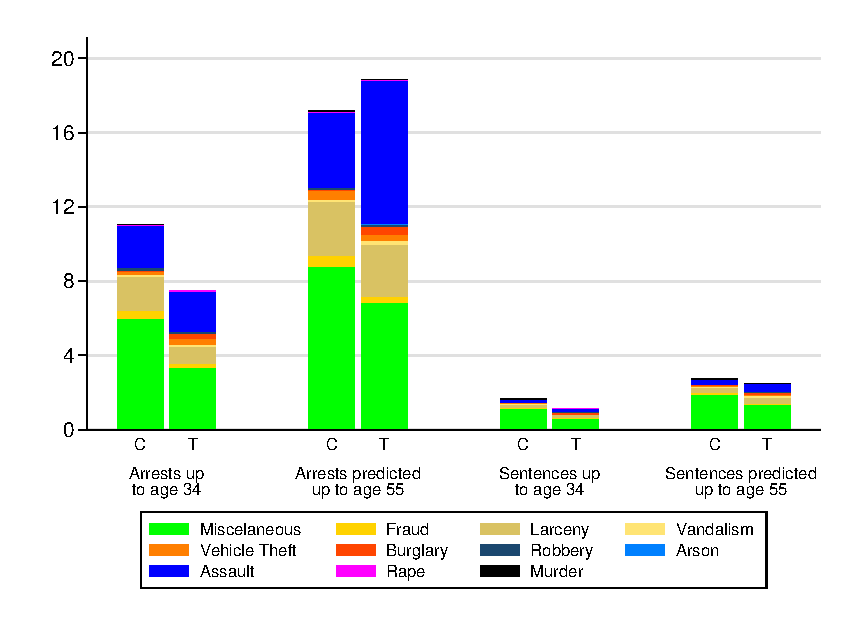
\includegraphics{AppOutput/Crime/predictions}}}
\floatfoot{
\footnotesize
\noindent Note: This figure continues Figure \ref{fig:datagraph}. It shows, for the control (C) and treatment (T) groups, the effects of adding predictions. The first pair of columns is the same as the fifth pair of columns in Figure \ref{fig:datagraph}. The second pair of columns includes the arrests that we predict. The third and fourth pairs of columns are the analogous pairs for sentences.
}\end{figure}

\subsection{Victimization Inflation}
\noindent Even though we have administrative data on crimes, we only observe the crimes that had justice system consequences (arrests or sentences). However, it is possible that the subjects committed more crimes than what we observe. Victimization Inflation (VI) is a method to capture benefits in crime reduction for crimes that did not result in justice system consequences.\footnote{\citet{Belfield_Nores_etal_2006_JHR,Heckman_Moon_etal_2010_RateofReturn}.} For most types of crimes in the U.S., there are many more victims than arrests or sentences. Using arrests as an example, VI assumes that those ``unpunished crimes'' were committed by the same people who were arrested for crimes of the same type, and in the same proportion. The calculation of VI uses as an input the national ratios of total number of reported crimes over the number of arrests. VI assumes that those national ratios are also valid for each individual. Under those assumptions, it is possible to find the total number of crimes committed by a subject for a given type of crime as the total number of arrests for that type of crime multiplied by the estimated national ratios for that type of crime. We estimate the total number of victims using two methods, one based on arrests and one based on sentences. Given that the ``unpunished'' crimes are by definition unobserved, it is not straightforward to use a data-driven method to allocate them between those subjects with arrests, those with sentences, and those with neither arrests nor sentences. We calculate separate estimates for arrests and sentences and use the average of those estimates as our main estimate. \\

\subsubsection{Construction of the Total Number of Victims in the U.S.}

\noindent The numerator of the VI ratio is an estimate of the total number of crimes of a certain crime type committed in the U.S. We construct this estimate using two datasets. First, we use the National Crime and Victimization Survey (NCVS). It has self-reported data on victimization of crimes reported on the household level. The data are available from 1995 to 2012. We also use the Uniform Crime Reporting Statistics (UCRS), which contains all crimes committed against households, individuals, and businesses that are reported to the police. These data are available from 1960 to 2013. Given that these two datasets independently underestimate the total number of crimes, but likely have significant overlap between them, we choose the highest estimate among both datasets for each type of crime. We refer to this estimate, $\overline{V_{j,t}}$, as the total number of victims in the country for type of crime $j$ in year $t$. \\

\subsubsection{Construction of the Total Number of Arrests in the U.S.}
\noindent The denominator of the VI ratio is an estimate of the total number of arrests of a certain type committed in the U.S. We have data from the ``National Arrests Analysis Tool'' of the National Bureau of Justice Statistics. These data are available from 1980 to 2012, which spans the years of all crimes that we observe in the ABC data. There is one problem with this dataset that we consider relatively minor: not all law enforcement agencies report the number of crimes (there are dozens of agencies that can legally arrest in the U.S.). However, as a large majority of them report the numbers of crimes, and because we are using national estimates, this should not greatly affect our calculations. We use these data to create $\overline{A_{j,t}}$, the total number of arrests in the country for type of crime $j$ in year $t$. \\

\subsubsection{Victimization Inflation Factors} 

\noindent Figure~\ref{fig:victim1} and Figure~\ref{fig:victim2} show the VI factors calculated by year. The ratios in the charts are constructed as $r_{j,t}=\frac{\overline{V_{j,t}}}{\overline{A_{j,t}}}$. In practice, we use an average of all the yearly measures in our calculations given that this exercise imputes unobserved crimes that do not have a clearly defined date. This average of all the yearly measures is given by $r_j=\Sigma_{t=t_0}^{T}r_{j,t}/T$, and has more precise estimates of the ratio. The VI factors we use for sentences are equal to the factors used for arrests, multiplied by the arrests-to-sentences ratios discussed above. Below, we will discuss combining these different estimates as per our arrest-based and sentence-based methodology. For sentences, we have data from the National Judicial Reporting Program (NJRP). These data are available from 1986 onwards. Using this dataset, we construct $\overline{S_{j,t}}$, the total number of sentences in the country for type of crime $j$ in year $t$. \\

\begin{figure} [H]
\caption{Victims-to-Arrests Ratios by Crime}
\centering \label{fig:victim1}
{\scalebox{0.8}{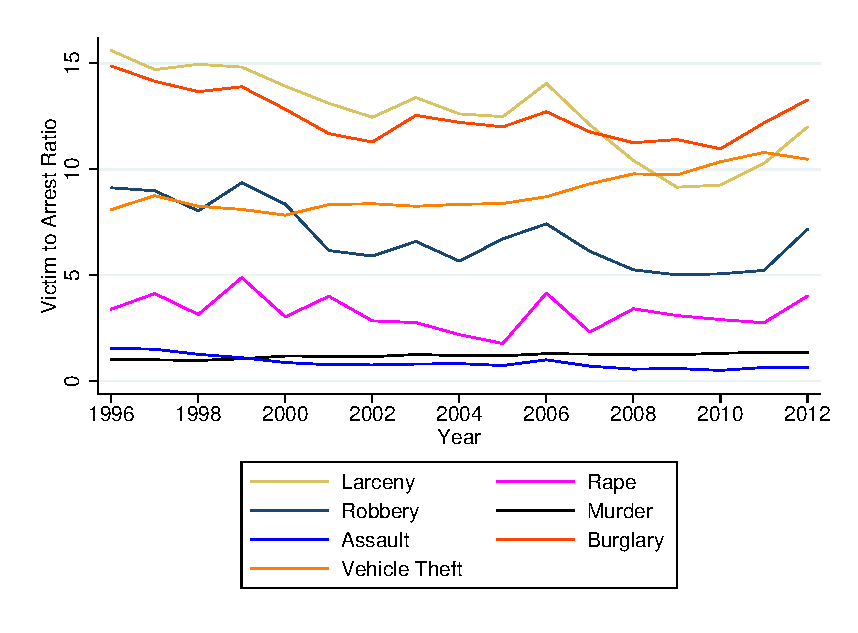
\includegraphics{AppOutput/Crime/v-to-a-ratios}}}
\floatfoot{
\footnotesize
\noindent Note: This figure shows, by year and type of crime, the number of victims (estimated from the NCVS and the UCRS datasets) divided by the number of arrests (estimated from the National Arrests Analysis Tool from the NBJS). In practice, we use a single number for each type of crime, which is an average across years.\\
}
\end{figure}

\begin{figure} [H]
\caption{Arrests-to-Sentences Ratio by Crime}
\centering \label{fig:victim2}
{\scalebox{0.8}{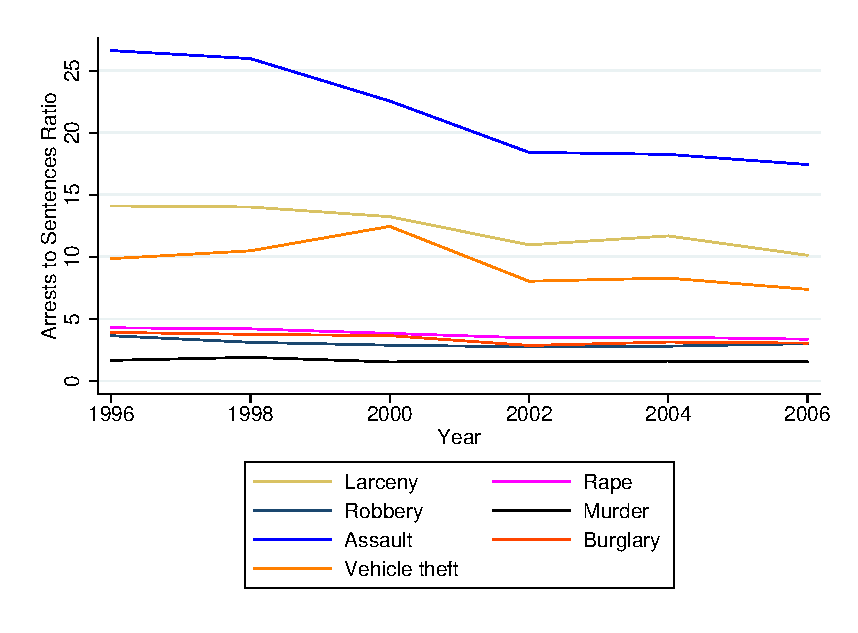
\includegraphics{AppOutput/Crime/a-to-s-ratios}}}
\floatfoot{
\footnotesize
\noindent Note: This figure shows, by year and type of crime, the number of arrests (estimated from the National Arrests Analysis Tool from the NBJS) divided by the number of sentences (estimated from the National Justice Reporting Program). In practice, we use a single number for each type of crime, which is an average across years. \\
}
\end{figure}

\subsubsection{Effects on Number of Crimes, After Victimization Inflation}
\noindent Figure \ref{fig:count-vi} shows the effects of VI on our estimates of the number of crimes committed. Note that the magnitudes in the axis are much larger than those of previous charts. The largest effects are for larceny, which is common in the data and has a victims-to-arrests factor of 12.6, the largest factor of all the categories of crime used in the paper. Given that the victim cost of larcenies is low, it affects the estimates less than what this chart suggests. \\

\begin{figure}[H]
\caption{Effects on Number of Crimes, After Victimization Inflation}
\centering \label{fig:count-vi}
{\scalebox{0.8}{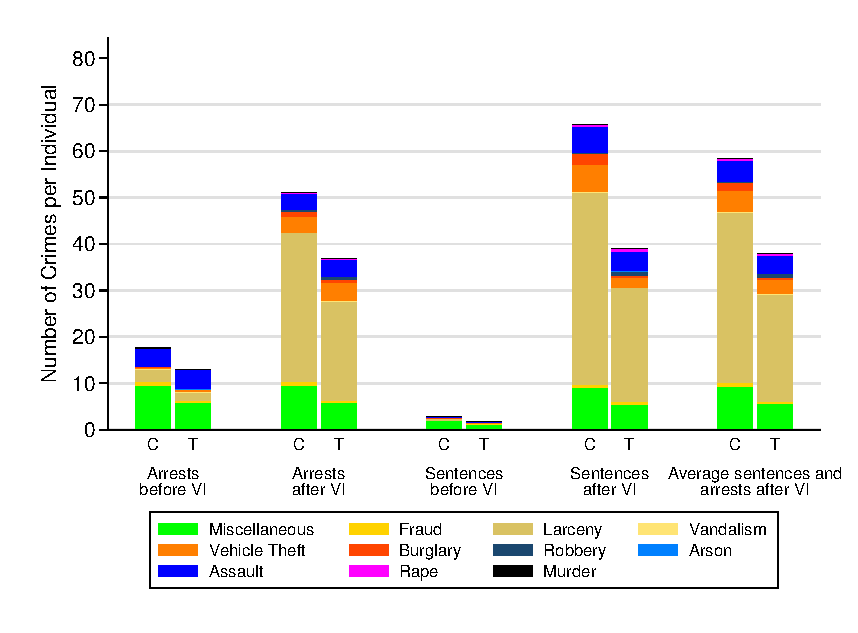
\includegraphics{AppOutput/Crime/vi}}}
\floatfoot{
\footnotesize
\noindent Note: This chart continues Figure \ref{fig:predictions}. It shows, for the control (C) and treatment (T) groups, the effects of adding victimization inflation (VI). The first pair of columns is the same as the second pair of columns in Figure \ref{fig:predictions}. The second pair of columns expand the arrests to account for VI. The third pair of columns is the same as the fourth pair of columns in Figure \ref{fig:predictions}. The fourth pair of columns expand the sentences to account for VI. The last pair of columns averages the second and the fourth pairs of columns in this chart. \\
}
\end{figure}

\noindent While the assumptions required for the victimization inflation methodology are strong, we argue that this is the best approximation for a total toll of crime's costs. The highest victims-to-arrests ratio shown in the figures are sensible and are not for the most costly categories of crime in the data, which stabilizes the estimates. \\

\subsection{Literature on Costs of Specific Crimes}
\noindent There are many methods to estimate unit costs of representative crimes, and many studies presenting estimates.\footnote{\citet{Cohen-Bowles_2010_Estimating-Cost-Crime} and \citet{McCollister_etal_2010_DAD} give comprehensive reviews of the state of the literature.} In this document, we only review the literature related to the inputs necessary for this paper. \\

\noindent We start by classifying the costs of crime, which is necessary to later discuss the methods to estimate the costs. Then, we present the two general types of methodologies that are used to estimate the total costs of crime: the Top-down methodologies and the Bottom-up methodologies. The former attempts to quantify the value that people put into \emph{ex-ante} prevention of crime, while the latter attempts to gather \emph{ex-post} all sources of costs that crime generates. The difference between these two methods can be large: \cite{Cohen-Bowles_2010_Estimating-Cost-Crime} show that for the particular case of estimates of the cost of rape, the top-down approach gives a value that is twice as large as the value given by most bottom-up studies. Other studies give cost estimates that are more homogeneous between these two approaches.\\

\subsubsection{Classifying the Costs of Crime}
\noindent Some methodologies used to estimate costs of crime are only able to capture some types of costs, and it might not even be clear what other methodologies are capturing. Some important types of costs are: \\
\begin{itemize}
\item Costs to the victim that can be directly quantified, such as medical bills, property losses, and lost productivity.
\item Costs to the victim that cannot be observed, such as pain and suffering.
\item Costs to the community in terms of prevention of crime, such as alarms, avoidance behavior, and police presence.
\item Costs to the community in terms of fear.
\item Costs to the community in terms of the criminal justice system, especially imprisonment.
\item Costs to the offender in terms of lowered productivity, such as forgone wages.
\end{itemize}

\subsubsection{Bottom-up (BU) Methodologies}
\noindent These approaches sum each type of cost that is imposed after the crime has been committed. The most well-known studies combine direct (also known as tangible) costs of the crimes with intangible costs. Tangible costs are everything that can be directly measured by observation, such as foregone wages, hospital costs, and police expenditure. Intangible costs are subjective, like pain and suffering. One way to measure these costs is using jury awards. For example, a jury award given as a result of an arm broken at a construction site can be used as a proxy of the intangible cost of having an arm broken in an assault.\footnote{This was first used in \citet{cohen_1988_Pain-Suffering}, and has been extensively used in BU studies after that. \citet{Miller_Cohen_ea_1996_BOOKvictim} improved on previous estimates by using jury awards specifically coming from criminal cases.} The problem of these approaches is that many of the costs of crime are not directly imposed on the victim and are hard to quantify, such as the ``fear of crime,'' the increased expenditure on crime prevention, and the negative impact of imprisonment on the community. \\

\subsubsection{Top-down (TD) Methodologies}
\noindent The other way to estimate the cost of crime is using TD methods, based on eliciting willingness to pay for avoiding crimes. The main advantage of these methods is that, in principle, they consider costs that are hard or impossible to measure directly, such as the cost of fear, avoidance behavior, and expenditures in preventative measures. There are three main methodologies for this approach, which we now briefly describe. \\

\begin{enumerate}
\item Stated Preferences. This basic method elicits the willingness to pay for hypothetical programs that would reduce crime nationwide for a sample of people.\footnote{\citet{Cohen_Rust_etal_2004_Criminology}.} Being an example of a TD methodology, it is expected that the costs obtained by this method would include factors that affect the community, and that are hard to capture, such as fear. However, it is unclear whether people consider factors like the cost of the justice system in their answers to these questions. An obvious caveat of this method is that people might not answer the real amount they would be willing to pay in these surveys.
%Then, multiplying that willingness to pay by the number individuals that would contribute, the total WTP for a certain reduction in crime is obtained. Dividing that total WTP by the number of crimes that would be avoided (number of crimes committed times the hypothetical effectiveness of the program), it is possible to find the WTP to avoid a particular crime.
\item Revealed Preferences. This method infers the value that individuals assign to crime reductions from market transactions. The most standard way to calculate these estimations is running regressions to explain the total price of houses with several factors, including the rates of crime in the area. Those parameters associated with the crime rate are considered the revealed valuation of avoiding crimes.\footnote{\citet{Thaler_1978_Value-Crime-Control}.} One weakness of this method is that it assumes that people are well-informed on the crime rates in an area. Another problem is that, in absence of extremely large and rich data on crimes and housing prices, it is not possible to separately identify the costs of different types of crimes. To the best of our knowledge, no paper has yet been able to convincingly obtain estimates per type of crime with this method.
\item Life Satisfaction. For this method, people are surveyed about their preferences between different life conditions, in which several different factors are considered. Some of those factors are income and rates of crime. By doing so, people implicitly associate monetary values to the levels of crime in the communities they would live in.\footnote{\citet{ Moore_etal_2006_Cost-of-Fear,Moore_2006_Value-Reducing-Fear}.}
\end{enumerate}

\subsubsection{Costs Used in this Study}
\noindent To summarize, both approaches have strengths and weaknesses: the TD approaches are more likely to reflect costs to the community (e.g. fear and anxiety, avoidance behavior, and protective measures) and better capture the spirit of a prevention program. However, in practice TD estimates rely on strong assumptions, and there are methodological issues associated with obtaining detailed values for the different types of crimes. It is also possible that when people answer the survey used for TD calculations they include some costs that we are including separately, such as justice system costs, and risk of death from non-murder crimes, while BU does not include them. Given those considerations, and the lack of TD costs for some categories of crime, we use BU costs for our main estimates. For completeness, we present cost estimates using both approaches. We choose \cite{Cohen_Rust_etal_2004_Criminology} as representative of the TD approaches, and \cite{McCollister_etal_2010_DAD} as representative of the BU approaches. In terms of timing, both of these studies match well with the ABC and CARE data. The bulk of crimes in the ABC and CARE data occurred between the late 1990s and early 2000s. While \cite{Cohen_Rust_etal_2004_Criminology} do not report the exact year of their survey, they use Census 2000 figures for their estimates. Even though \cite{McCollister_etal_2010_DAD} is a more recent study, many of the productivity estimates that their costs are based on are taken from papers using data from years with more crimes the late 1990s and early 2000s. The costs in those studies are presented in Table \ref{tab:individual-crime-cost}. Notice that there are some strong differences in the cost of crimes, such as assault, burglary, and especially robbery. \\

%The fact that \cite{cohen1994costs} and \cite{miller1996victim} are relatively old studies is an advantage rather than a problem. The studies better reflect the costs of crimes in those years, which are part of the period in which most crimes were committed by subjects in the ABC and CARE data. More recent estimates will be based on assumptions about productivity and costs that are not representative of the losses relevant for this study. These studies are complementary, as \cite{miller1996victim} quantifies cost to victims (productivity, medical care, mental health care, police/fire services, social services, property loss and quality of life damages), while \cite{cohen1994costs} provides a quantification of criminal justice system costs. Importantly, this study distinguishes between sources of costs, so we can impute our own cost estimates to sentences, knowing precise information about time in jail for our sample. The most recent study  \citep{mccollister2010cost} is necessary because it considers some types of crimes omitted in the previous papers.

\begin{table}[H]
\begin{threeparttable}
\caption{Unitary Costs of Crime for Victims} \label{tab:individual-crime-cost}
\begin{tabular}{lcc}
\toprule
Crime				&Top-Down Approach	&Bottom-Up Approach	\\
					& \cite{Cohen_Rust_etal_2004_Criminology}&\cite{McCollister_etal_2010_DAD}\\ \midrule
Arson				&					&12,093			\\
Assault				&95,200			&16,132 			\\
Burglary			&34,000			&1,467 			\\		
Fraud				&				&0				\\
Larceny				&				&528 				\\
Motor Vehicle Theft	&				&6,699 			\\
Murder				&13,192,000		&9,286,200 		\\
Rape				&322,320			&224,021 			\\
Robbery				&315,520			&7,273 			\\
Vandalism			&					&0				\\ \bottomrule
\end{tabular}
\begin{tablenotes}
\item Note: All amounts are in 2014 USD. The amounts reported in \cite{McCollister_etal_2010_DAD} for non-murder crimes have the extra cost for risk of death and the cost of a crime career removed (both were obtained from correspondence with the author). Risk-of-death costs do not apply, because we know the outcomes of the crimes. Crime-career costs do not apply, as we directly observe the income of the individuals. These costs also don't include police and legal system costs, as those are imputed separately and only for the cases for which individuals were arrested or sentenced.
\end{tablenotes}
\end{threeparttable}
\end{table}

\subsubsection{Timing of Effects: Incidence vs. Prevalence}
\noindent We would like to discount the costs of crime according to whether they were \textit{incurred} during a particular age of ABC and CARE subjects, because those values should be discounted at a different rate than costs incurred later, even if both costs were \textit{imposed} in the same year. Thus, the value of the imprisonment is discounted year-by-year. We have no information about the timing of costs for victims, so the value of the different crimes for the victims are discounted according to the time they were imposed (the time of the crime's occurrence). \\

\subsubsection{Costs of Imprisonment}
\noindent Unlike previous studies, we observe the sentences of the ABC and CARE subjects. This allows for a precise estimation of the costs of imprisonment. For the cost of jail and state prison, we use estimates from the \citet{US-Justice_1988_Report-Crime-Justice}. In 2014 USD, these costs are \$25,338 for a year in a state prison, and \$21,939 for a year in jail.
It is important to clarify that we only include costs of the justice system for the crimes that are known by the justice system, not for the crimes that we impute through victimization inflation. \\

%%%%%%%%%%%%%%%%%%%%%%%%%%%%%%%%%%%
\subsection{Effects on Costs of Crime}

%\subsubsection{Criminal Behavior.} The results show that there are clear reductions in the amount of crime committed between the control and treatment groups. This holds true for the majority of the categories of crime. The exceptions were Vehicle Theft, Assault, Robbery, and Arson. The visualization of the ABC and CARE data in Figure \ref{tab:lifehistory} represents the life history of each of the individuals within the ABC study that committed at least one crime, with each dot as an offense and each line as a period of incarceration. Also shown are the most serious crimes committed in the ABC data, including a habitual felon, manslaughter, and indecent liberties with children. The largest treatment effects occurred in cases of Miscellaneous, Fraud, and Larceny crimes. In sentences alone, there was a 46.3\% reduction in the number of cases, and in arrests, there was a 39\% reduction in cases for those in the treatment group compared to the control group. There are substantially fewer arrests for the individuals in the treatment group, and although there are still a few who committed a series of crimes, many did not have arrests at all.
%numbers from combined_datasetv3

\subsubsection{Effects on Costs Before Victimization Inflation}  Figure \ref{tab:diff-costs} presents the estimated costs per type of cost before victimization inflation.
\noindent There are clear positive effects for the treatment group in terms of reductions in the costs of crime. Those reductions are almost exclusively given by the large effect of the murder case we observe in the control group (note that murder also appears in the treatment group costs because of the predictions). Comparing the bars in this figure, the costs from the justice system and from imprisonment are low compared with the victimization costs, even without victimization inflation. While the levels of the arrest-based estimates are higher than the levels of the sentence-based estimates for both the treatment and control groups, the impacts of the program are quite similar across both methods (Figure~\ref{tab:diff-costs}). \\

\begin{figure} [H]
\caption{Costs of Crime Before Victimization Inflation}
\centering  \label{tab:diff-costs}
{\scalebox{0.8}{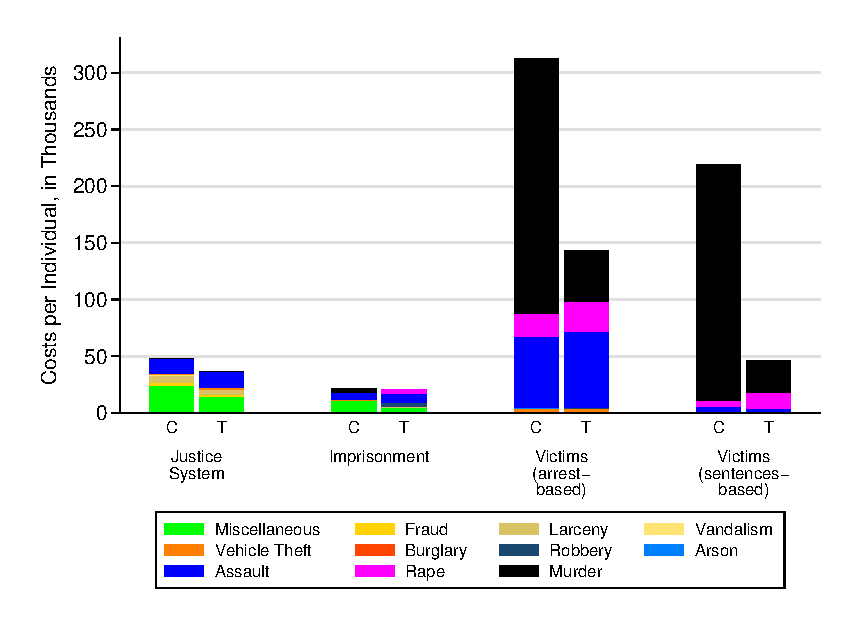
\includegraphics{AppOutput/Crime/different_costs}}}
\floatfoot{
\footnotesize
\noindent Note: This figure depicts the per capita cost for the different categories of costs and crimes we use, by control (C) and treatment (T). The first pair of columns adds up the justice system costs (including police) for all arrests inputed for each subject. The second pair of columns adds up the cost of Imprisonment. It is important to note that the costs are per capita, so there are individual cases that have much higher costs. The next two pairs of columns show the pre-victimization inflation estimates of number of crimes multiplied by the individual victim cost of the different crimes. The costs are taken from the Bottom-up approach in Table \ref{tab:individual-crime-cost}. All costs are in thousands of 2014 USD.\\
}
\end{figure}

\subsubsection{Effects on Costs After Victimization Inflation}

\noindent Figure \ref{tab:costs_vi} presents the data after applying the victimization inflation. As shown below, the inflation allows us to include a substantial amount of crime that otherwise would not have been considered. This chart shows that the treatment effects using arrest-based estimations are not substantively different from the ones using sentence-based estimations. Thus, to use all available information, we use the estimates based on the averages of the two for our analysis. \\

\begin{figure} [H]
\caption{Costs of Crime After Victimization Inflation}
\centering  \label{tab:costs_vi}
{\scalebox{0.9}{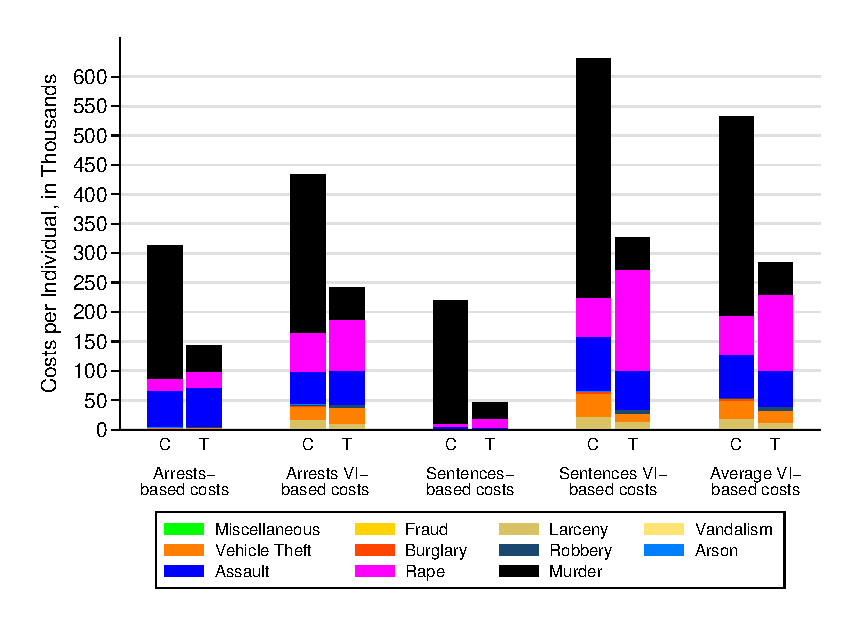
\includegraphics{AppOutput/Crime/costs_vi}}}
\floatfoot{
\footnotesize
\noindent Note: This figure depicts the per capita cost for the different categories of costs and crimes we use, by control (C) and treatment (T). The first two pairs of columns adds up all of the arrest-based costs for each subject and compares the pre- and post-victimization inflation costs. The third and fourth pair of columns compare the pre- and post-victimization inflation sentence-based costs. It is important to note that the costs are per capita, so there are individual cases that have much higher costs. The next two pairs of columns show the post-victimization inflation estimates of number of crimes multiplied by the individual victim cost of the different crimes. The costs are taken from the Bottom-up approach in Table \ref{tab:individual-crime-cost}. All costs are in thousands of 2014 USD.\\
}
\end{figure}

\noindent We consider the impact on murder as a consequence of the program rather than a statistical coincidence. We use as precedent the cost-benefit analysis of Perry in which three control group individuals and one treatment group individual committed murders.\footnote{\citet{Heckman_Moon_etal_2010_RateofReturn}.} \\

Some of the sources of cost estimates, such as the more serious crimes, result in volatile estimates due to the small sample sizes. Our estimations of the standard errors associated with the objects of interest in this paper---the present value of the program and the internal rate of return---consider those sources of volatility. Ultimately, the benefit-cost analysis is a unidimensional summary of benefits of a program, and specific flows of benefits with high variability enter naturally into the process of aggregation. \\

%\begin{table}[H]
%\begin{threeparttable}
%\caption{Effects on Total Costs}\label{tab:apx_impact-costs-total}
%{
\def\sym#1{\ifmmode^{#1}\else\(^{#1}\)\fi}
\begin{tabular}{l*{1}{ccccc}}
\hline\hline
                    &Mean Control&Mean Treatment&  Difference&           $t$& $p$-value\\
\hline
Total Costs for All Crimes&      246967&      150511&       96456&        0.64&        0.26\\
Costs Miscelaneous  &       14769&        8058&        6711&        1.45&       0.075\\
Costs Fraud         &        1095&         635&         460&        0.79&        0.21\\
Costs Larceny       &       11793&        7910&        3883&        0.83&        0.20\\
Costs Vandalism     &         260&         193&          67&        0.43&        0.34\\
Costs Vehicle Theft &       14866&       10327&        4540&        0.39&        0.35\\
Costs Burglary      &        1253&         291&         962&        1.36&       0.088\\
Costs Robbery       &        1091&        4500&       -3408&       -1.13&        0.87\\
Costs Arson         &         161&         152&          10&       0.093&        0.46\\
Costs Assault       &       38830&       33484&        5346&        0.30&        0.38\\
Costs Rape          &       35388&       65721&      -30333&       -0.43&        0.67\\
Costs Murder        &      127460&       19242&      108218&        0.87&        0.19\\
\hline\hline
\end{tabular}
}

%\begin{tablenotes}
%\item  Note: this table presents the treatment effects of ABC on total costs of crime per capita, including Victimization Inflation. All costs are in 2014 USD. We present one-sided $p$-values.
%\end{tablenotes}
%\end{threeparttable}
%\end{table}

\subsection{Sensitivity Analyses Using Alternative Cost Estimates}
\noindent So far, we study several ways to construct our estimates: \\

\begin{enumerate}
\item We show that not matching the different crime datasets could reduce the number of crimes, but that the general patterns are stable, and no dataset is especially influential.
\item We show that not including predictions up to age 50 noticeably reduces the number of crimes, but the general patterns are not modified.
\item We show estimates using arrest-based estimations versus sentence-based estimations, and find that the differences are large in terms of the number of crimes before victimization inflation, but small after it, and do not substantially change the total benefits calculations.
\end{enumerate}

\noindent In Figure \ref{fig:costs_schedules}, we present additional deviations from our main estimates. In particular, we show how the estimations change when two different cost schedules are used: (i) Top-down costs, and (ii) Bottom-up costs, assuming that the costs of murders and rapes are identical to the cost of an assault. We also note that BU costs are a ``conservative'' option in the sense that the effects of the program are higher using TD costs. We can also see that with no murders and rapes, the effect of the program on crime is still positive, but much smaller than when those crimes are considered. \\

\begin{figure} [H]
\caption{Different Cost Schedules}
\centering  \label{fig:costs_schedules}
{\scalebox{0.9}{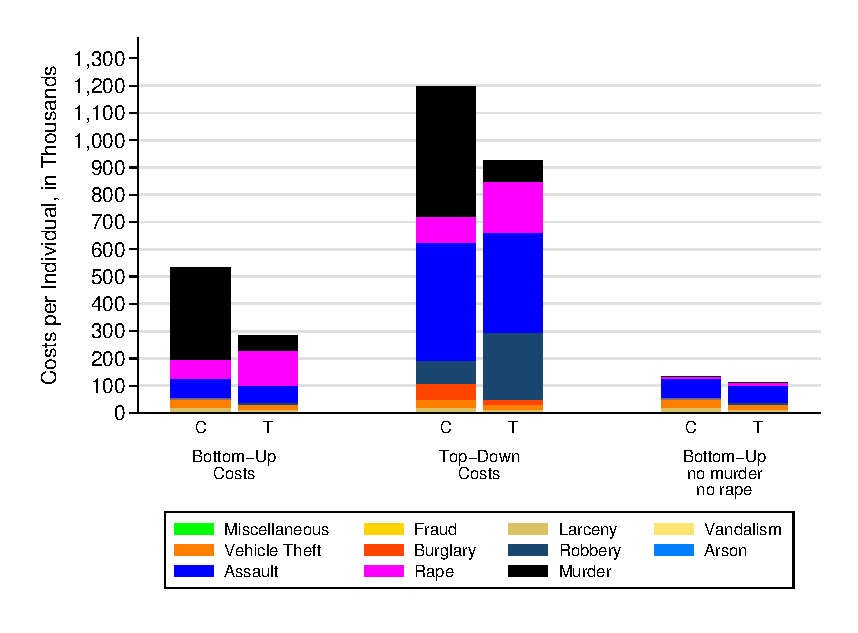
\includegraphics{AppOutput/Crime/bu_td_nomur}}}
\floatfoot{
\footnotesize
\noindent Note: This figure depicts the per capita cost for the different categories of costs and crimes we use, by control (C) and treatment (T). It presents some sensitivity analyses. The first pair of bars represents costs using the Bottom-up approach in Table \ref{tab:individual-crime-cost} to determine individual costs of crime. The second pair of bars represents costs using the Top-down approach in Table \ref{tab:individual-crime-cost} to determine individual costs of crime. The third pair of bars uses the Bottom-up approach, but replaces the values of murders and rapes with that of assaults.\\
}\end{figure}

\noindent Finally, in Figure \ref{fig:crime_discounting}, we present the effect that discounting and applying deadweight loss has on our estimates. The first pair of bars represents the cost estimates that are not discounted, the second pair of bars represents the discounted costs, and the third pair of bars represents the discounted costs including deadweight losses. It is clear that the effect of discounting is substantial, approximately halving the total cost estimates. The effect of applying deadweight loss barely changes the estimates. The effect of deadweight loss is most noticeable in the value of miscellaneous crimes, which are only public costs. Regardless, its impact in the overall costs is minor. \\

\begin{figure} [H]
\caption{Effect of Discounting Crime Costs}
\centering  \label{fig:crime_discounting}
{\scalebox{0.9}{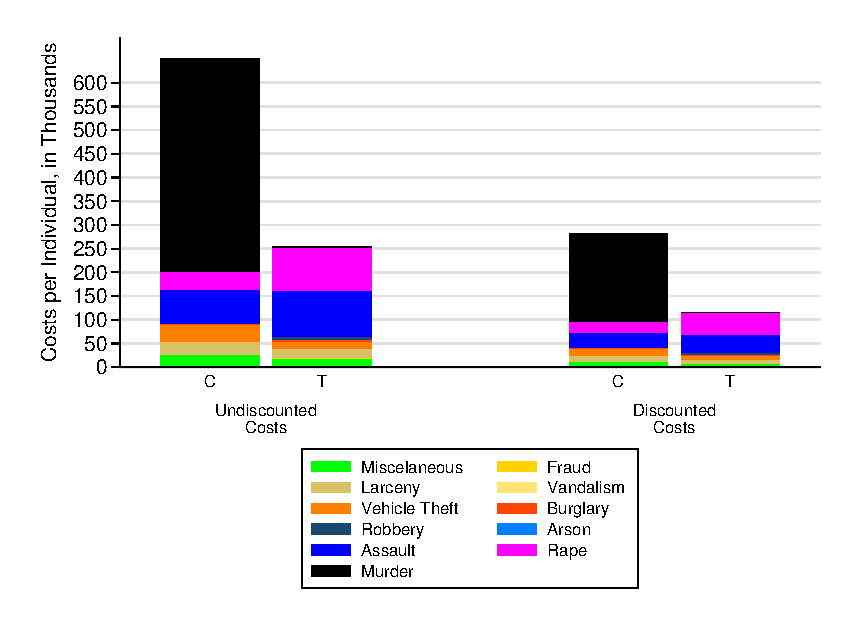
\includegraphics{AppOutput/Crime/crime_discounting}}}
\floatfoot{
\footnotesize
\noindent Note: This figure depicts the per capita cost for the different categories of costs and crimes we use, by control (C) and treatment (T). The discounted costs use 3\% as a discount factor, and are discounted to birth. The deadweight loss (DWL) adjustments increases the costs from justice system and imprisonment by 50\%. All costs are in thousands of 2014 USD.\\
}\end{figure}


\setcounter{figure}{0}  \renewcommand{\thefigure}{F.\arabic{figure}}
\setcounter{table}{0}   \renewcommand{\thetable}{F.\arabic{table}}
\section{Health Outcomes in the Future Adult Model (FAM)} \label{appendix:health}

\noindent \textbf{[JJH: The last battle zone!]}

\noindent \textbf{[JLG: I have reworked this version, based on your comments and on my conversations with Bryan and Duncan. I have gotten rid of a lot of the extensive verbal introduction and many other verbal details that now have become schematic and clear with the presentation of what we estimate and the big tables that I generated.]}

Our methodology to forecast and monetize health outcomes is a modified version of Section~\ref{section:cbamethodology}. When studying labor income, a first-order autoregressive model is a helpful device to simplify a complex reality and produce forecasts. As it turns out, in the paper we find that model to perform well under a variety of testable implications. 

When studying health, a modified version is needed because there is abundant state interdependency in health outcomes. We use a dynamic microsimulation model (the Future Adult Model - FAM) as laboratory to estimate health-state occupancy probabilities and to predict other health and economic outcomes. With this in hand, we forecast the health trajectories of the ABC/CARE individuals. In Section~\ref{section:cbamethodology}, we initialize the forecast of labor income using labor income at age 21. In this appendix, we use a ABC/CARE rich age-30 interview and a health follow-up conducted when the subjects were in their mid-30s to initialize the forecast of the health trajectory. We then monetize health outcomes using quality-adjusted life years and medical costs.\footnote{This microsimulation model is an extension of the model used by \citet{Prados_etal_2015_How-Much-Can-Education}; the technical details are described in \citet{Goldman_etal_2015_Future-Adult-Model}. Both models are related to the Future Elderly Model (FEM), which is a microsimulation tool originally developed to examine the health and health care costs among the elderly Medicare population \citep{Goldman_etal_2004_RAND-Report_Health-Status-Elderly}. It has been used extensively to assess health and disease prevention scenarios: FEM has been used to assess the future costs of disease, the benefits of preventing disease among older population, the consequences of new medical technologies, trends in disability, and the fiscal consequences of worsening population health (see \citet{Goldman_etal_2004_RAND-Report_Health-Status-Elderly}, \citet{Lakdawalla_etal_2004_Health-and-Cost}, \citet{Goldman_etal_2005_HA}, and \citet{Zissimopoulos_etal_2014_Delaying-Alzheimers}). The main differences with FEM are that the model we use starts with cohorts of individuals at age 30 instead of 50, and that it simulates more outcomes than FEM, because they are important to explain health outcomes and medical expenditure at younger ages, like evolution of partnership and marital status, work status, and family size.}

\noindent Before providing formal details, we summarize the data sets used, as well as variable construction and imputation assumptions.

\subsection{Data Sources} \label{section:data}
\noindent FAM uses data from ABC/CARE follow-up surveys to set the initial state of the cohort.
The transition model parameters are estimated from the 1997 to 2013 waves of the Panel Study of Income Dynamics (PSID).
We supplement the PSID with data from the Health and Retirement Study (HRS). We use the National Health and Nutrition Examination Survey (NHANES)
to account for differences between measured and self-reported BMI.
To estimate medical care costs associated with health conditions, we use the Medical Expenditures Panel Survey (MEPS) and the Medicare Current Beneficiaries Survey (MCBS).


\subsubsection{PSID}
\label{section:data_psid}
%The Panel Survey of Income Dynamics (PSID) is a longitudinal household survey containing between 5,000 and 8,500 families in each wave, which began yearly in 1968 and is fielded biennially since 1996. When appropriately weighted, the PSID is designed to be representative of U.S. households. The PSID provides extensive information concerning demographics, economic outcomes, health care access, health outcomes, and health behaviors (such as smoking history, alcohol consumption, and exercise habits). Health outcome variables include diagnosis of diabetes, heart disease, hypertension, lung disease, cancer, etc.

\noindent The Panel Study of Income Dynamics (PSID) provides extensive information concerning demographics, economic outcomes, health care access, health outcomes, and health behaviors (such as smoking history, alcohol consumption, and exercise habits). Health outcome variables include diagnosis of diabetes, heart disease, hypertension, lung disease, and cancer, among others.

\noindent We estimate the transition models using waves from 1997 to 2013. We create a dataset of respondents who have formed their own households, either
as single heads of households, cohabiting partners, or married partners. These heads, wives, and husbands respond to the richest
set of PSID questions, including the health questions that are critical for our purposes. We use all respondents aged 25 and older.\footnote{While we use the full sample in our main analysis, we explored using a few different subsamples to better adapt to the demographics of the ABC/CARE subjects.}
The length of the PSID is a significant advantage, because we can include past health behaviors as explanatory variables for current health outcomes. This dataset provides adequate sample sizes to explore health outcomes of specific groups.
PSID does not follow individuals who are institutionalized in nursing homes or other long-term care facilities. To overcome this weakness, we pool the PSID sample with the HRS sample when
estimating mortality models.

\subsubsection{HRS}

\noindent The Health and Retirement Study (HRS) is a longitudinal panel that surveys a nationally representative sample of individuals over the age of 50 and their spouses every two years. When appropriately weighted, the HRS in 2010 is representative of U.S. households
where at least one member is at least 51 years old.
This study collects in-depth information about income, work, health, and medical expenditures. In our model, waves from 1998 to 2012 are pooled with the PSID for estimation of mortality and
widowhood models. The HRS data
are harmonized to the PSID for all relevant variables. Because the PSID does not follow respondents into nursing homes, we also use the HRS to estimate the model for nursing home residency. We use all cohorts in the dataset created by RAND (RAND HRS, version O) as the basis
for our analysis.

\subsubsection{MCBS}
\noindent The Medicare Current Beneficiary Survey (MCBS) is a nationally representative sample of aged, disabled,
and institutionalized Medicare beneficiaries. The MCBS attempts to interview each respondent twelve
times over three years, regardless of whether he or she resides in the community, a facility, or
transitions between community and facility settings. The disabled (under 65 years of age) and
very elderly (85 years of age or older) are over-sampled. The first round of interviewing was conducted
in 1991. Originally, the survey was a longitudinal sample with periodic supplements and indefinite
periods of participation. In 1994, the MCBS switched to a rotating panel design with limited periods
of participation. Each fall, a new panel is introduced, with a target sample size of 12,000 respondents. Each summer, a panel is retired. Institutionalized respondents are interviewed by proxy. The MCBS
contains comprehensive self-reported information on the health status, health care use and
expenditures, health insurance coverage, and socioeconomic and demographic characteristics of the
entire spectrum of Medicare beneficiaries. Medicare claims data for beneficiaries enrolled in
fee-for-service plans are also used to provide more accurate information on health care use and
expenditures. MCBS data from 2007 to 2010 are used for estimating medical costs and enrollment models.

\subsubsection{MEPS}
\noindent The Medical Expenditure Panel Survey (MEPS), which began in 1996, is a set of large-scale surveys of families and individuals, their medical providers, and employers across the U.S. The Household Component (HC) of the MEPS provides data from
individual households and their members, which is supplemented by data from their medical providers.
The HC collects data from a representative subsample of households drawn from the
previous year's National Health Interview Survey (NHIS). Since NHIS does not include the
institutionalized population, neither does MEPS; this implies that we can only use the MEPS to
estimate medical costs for the non-elderly (ages 25--64) population. Information collected during household
interviews include: demographic characteristics, health conditions, health status, use of medical
services, sources of medical payments, and body weight and height. Each year the household survey
includes approximately 12,000 households, or 34,000 individuals. Sample size for those aged 25-64 is
about 15,800 in each year. MEPS has comparable measures of socioeconomic status as those in PSID,
including age, race and ethnicity, educational attainment, census region, and marital status. We estimate medical expenditure
and utilization using data from 2008 to 2010. We use waves from 2001 to 2003 to estimate models of quality-adjusted life years (QALYs), due to availability of EQ-5D instrument in these waves.\footnote{Section \ref{section:FAM_models} explains the estimation of the QALY model.}


\subsubsection{NHANES}
\noindent
The National Health and Nutrition Examination Survey (NHANES) targets a nationally representative sample of approximately 5,000 individuals in each year since 1999. The data collected includes responses to interview questions about demographics, disease conditions, height, and weight, as well as physical measurement of BMI. We use NHANES years 2002 to 2010 to estimate a model for imputing measured BMI from self-reported BMI. The methodology is described in Section \ref{section:FAM_ABC_impute}.

\subsubsection{ABC/CARE}
\noindent FAM uses ABC/CARE data to initialize the state of each ABC/CARE subject when they enter into the simulation.
These data are taken from the the parental interviews at various subject ages from birth to age 21; age-30 subject interview; and mid-30s biomedical survey.
The goal is to have each subject's initial state in the simulation match their status at the age-30 subject interview. However, because several key FAM inputs are not available at the age-30 interview, we use PSID or ABC/CARE surveys corresponding to other ages to impute missing elements. These imputations are discussed in Section \ref{section:FAM_ABC_impute}.

\paragraph{Variable Construction and Imputations}
\label{section:FAM_ABC_impute}

% \todo would be nice to have a table that summarizes imputed variables at age 30, imputation method, and number of missing subjects

\noindent Marital status transitions and childbearing in FAM are affected by the subject's mother's education level. The ABC/CARE age-30 subject interview did not ask about mother's education, but the ABC age-21 parent interview did.
For ABC subjects, we assume that each subject's mother had the same education level at the age-30 subject interview as what was reported in the age-21 parent interview. For CARE subjects, we impute mother's education from an ordered Probit model using race, ethnicity, education, disease conditions, employment status, presence of a health-related work limitation, and a self-report of whether or not the subject was ``poor'' as a child.  The model is estimated using age 30 to 31 PSID subjects with birth years between 1945 and 1981. Each of the model covariate values are taken from the CARE age 30 interview. At the beginning of each simulation repetition, an education level is randomly drawn from the probability distribution for each CARE subject and assigned to be the mother's education level.

\noindent Many FAM transition models depend on a three-level measure of parents' economic status when the subject was a child.
This is based on the PSID question: ``Were your parents poor when you were growing up, pretty well off, or what?''
The three possible responses are ``poor,'' ``average''/``it varied'', or ``pretty well off.''
This question is not included in the ABC/CARE interviews, but because preliminary eligibility for the program focused on children from high-risk backgrounds, based on socioeconomic factors, the value of this variable is set to ``poor'' (when growing up) for all ABC/CARE subjects.

\noindent All FAM transition models depend on demographics of the subject, including whether or not the subject is Hispanic.
This information is not available in the ABC/CARE data, but it is assumed that none of the ABC/CARE subjects are Hispanic.\footnote{Census data on Hispanics in North Carolina were not available for 1970 and 1980, but Hispanic migration into this state is more recent than in other regions, and as late as 1990, only 2\% of the North Carolina poor were Hispanic \citep{Johnson_2003_Changing-Poverty}.}

\noindent Most FAM models depend on smoking status. Employment status affects FAM transitions in marital status, childbearing, claiming of disability insurance (DI) and supplemental security income (SSI), and type of health insurance.
One male in the ABC control group is missing smoking status and, although known to be not working, is also missing specific employment status (unemployed or out of the labor force).
 We use a multinomial logit model to jointly estimate the probability of each combined smoking and employment category among 25- to 35-year-olds in the PSID who were not working. At the beginning of each simulation repetition, we use a Monte Carlo random draw generated from this distribution to assign this subject's smoking and employment statuses. This same subject is also missing information about binge drinking. A separate binary Probit binge drinking model was estimated using the age 25--35 PSID data. A Monte Carlo random draw is taken according the Probit probability to forecast binge drinking behavior at the beginning of the simulation.

\noindent BMI affects FAM transitions in health, functional status, employment, and smoking.
The FAM transition models are estimated with BMI computed from self-reported height and weight in the PSID.
The only BMI data in ABC/CARE come from height and weight measured during the health interview. This interview took place at roughly age 30 for CARE subjects, and at age 34 for ABC subjects.
This poses two challenges.
First, self-reported BMI can be biased by factors such as actual height and weight, gender, and race.\footnote{\citet{Cawley_2004_JHR}.}
Second, it is possible that BMI could increase or decrease systematically in the years between the age-30 subject interview and the age-34 health interview.

\noindent To address the first BMI imputation challenge, we use a variation on the method of \citet*{Courtemanche_etal_2015_Adjusting-Body-Mass} to impute measured BMI in the PSID.
While the method in \citet{Courtemanche_etal_2015_Adjusting-Body-Mass} works for importing height and weight, we apply the following specification to directly model BMI. Using respondents aged 30 to 40 in the 2002-2010 NHANES waves, we forecast measured BMI from percentile ranks of self-reported BMI using the model specification in \citet{Courtemanche_etal_2015_Adjusting-Body-Mass}. Three variations
on the spline interactions of \citet{Courtemanche_etal_2015_Adjusting-Body-Mass} are also considered. After estimating these models using NHANES data, covariate values from the PSID
age 30--34 data in years 2002--2013 are used to impute measured BMI values for PSID respondents. A Kolmogorov-Sminov (K-S) test and a visual inspection of smoothed histograms are used to compare the distribution of PSID imputed values to the distribution of observed values in the NHANES estimation sample. The model specification used for imputation has the smallest K-S distance between the two distributions.

\noindent After imputing values of measured BMI for PSID respondents age 30--34, we turn to the second problem: accounting for systematic trends in BMI from the age 30 interview to the health interview. The goal is to have a model that maps from measured BMI at the health interview around age 34 to self-reported BMI at the age 30 interview. Employing the longitudinal structure of PSID, we match each respondent's first interview between age 30--32 with their imputed measured BMI between ages 33--40. We then estimate a model using self-reported BMI between ages 30--32 as the response variable and imputed measured BMI at ages 33--40, the age when BMI is actually measured, along with other variables observed at age 30 as explanatory variables. This imputation model is applied to any ABC/CARE subject who has their health interview at least one year after their age 30 interview.

\noindent For ABC/CARE subjects who have their health interview within one year of the age 30 interview, we assume that any systematic time trends in BMI are too small to have any practical significance. However, we still need to convert the imputed measured BMI to a self-reported value for compatibility with other transition models estimated in PSID. This model is estimated on ages 30--32 in the PSID and uses covariates from the age 30 interview along with imputed measured BMI to forecast self-reported BMI.

\noindent At the beginning of each simulation repetition, we choose the appropriate model to impute self-reported BMI for each ABC/CARE subject based on the time between their age 30 interview and their health interview. Their expected BMI is estimated from this model. A Monte Carlo Normal random draw is generated using the subject's expected BMI and the estimated variance from the model. This Monte Carlo draw is then assigned to be the subject's initial self-reported BMI in the simulation. Using BMI from the health interview limits the ABC/CARE subjects simulated in FAM to only those who have height and weight measurements in the health interview.

\noindent Subjects' health insurance coverage affects their medical costs.
FAM uses three categories of health insurance: none, public only, and some private.
Five ABC subjects and three CARE subjects were missing health insurance status.
Three cases were logically imputed by assuming that subjects have no health insurance if they do not know their insurance status and either go to an emergency room or community health clinic or do not go anywhere when they need health care.
In order to impute the insurance category for the remaining five cases, we use age 25--35 PSID data to estimate a Probit model for whether or not a subject had insurance.
The predictors were gender, earnings, marital status, self-reported health, employment status, and whether or not the subject had any biological children.
We use this model to compute the probability of having insurance at the start of the simulation (at the age-30 interview).
Then, we generate a Monte Carlo binary random variate according to this probability.
If the outcome is positive, the subject is assigned to have some private insurance.

\noindent FAM uses six Activities of Daily Living (ADLs) about which there is data in PSID: walking, dressing, eating, bathing or showering, getting in and out of bed or a chair, and using the toilet, including getting to the toilet.
FAM simulates the number of these ADLs in which the subject has difficulty.
ADL difficulties forecast FAM transitions in benefits claiming, mortality, employment status, insurance category, and nursing home residency.
FAM also transitions the count of difficulties among six Instrumental Activities of Daily Living (IADLs) from PSID: preparing one's own meals; shopping for personal toilet items or medicines; managing one's own money, such as keeping track of expenses or paying bills; using the phone; doing heavy housework, like scrubbing floors or washing windows; and doing light housework, like doing dishes, straightening up, or light housecleaning.
Both ADLs and IADLs are components of FAM's model for quality-adjusted life years (QALYs).
The ABC/CARE age-30 subject interview does not ask about ADLs or IADLs, but it does ask if the subject has a physical or nervous condition that keeps them from working.
PSID respondents are also asked this question.
We create an imputation model for each of these two measures using an ordered Probit model estimated on PSID respondents aged 25 to 35.
We use these models to compute the probabilities for each number of ADLs and IADLs. To start the simulation, we generate Monte Carlo random draws according to these probabilities and use them to assign the corresponding counts.

\noindent When a subject claims DI benefits, it affects their FAM transitions in employment status, insurance category, and Medicare enrollment.
DI claiming also affects medical costs.
SSI claiming affects FAM transitions in employment status.
Lastly, claiming Social Security retirement benefits affects FAM transitions in employment status and insurance category.
The ABC age-30 subject interview has a single yes/no question about claiming which asks: ``Currently are you receiving income from workman's compensation, disability, or Social Security benefits including Supplemental Security Income?'' CARE asks a similar question. The PSID has separate questions for each benefit type. We use a multinomial logit model to estimate the joint probability of each combination of DI and SSI claiming. The estimation uses PSID respondents aged 25 to 35 who were claiming at least one of the following benefits: workman's compensation, DI, or SSI. A Monte Carlo random draw generated from this distribution is used to assign each ABC/CARE subject's DI- and SSI-claiming status at the start of the simulation. One ABC subject is missing data about whether or not they were claiming and was assumed to not be claiming any benefits.

\noindent As discussed in Section \ref{section:FAM_models}, FAM uses different models to estimate medical costs depending on whether or not a subject is Medicare-eligible. Subjects can enroll in Medicare before the age of 65 if they are claiming DI. The cost estimates for Medicare-eligible subjects depend on the subjects' current disease status at the age-30 interview and their disease status two years prior to the interview. Unfortunately, ABC/CARE does not have disease data two years before the age-30 interview. It is assumed that all subjects do not have their disease conditions in the previous period.










% \todo we could add a table of all the FAM input variables (rows) and three columns, as-is, rule imputed, model imputed, with checkmarks to indicate how the data were derived

\subsection{Methods and Analysis}

% \todo capital income -- imputed, but not used as an outcome

% \todo we will include health conditions at age 30 in covariates of health dynamics

% \todo health as a child -- are we going to ignore this?

% \todo summarize disease conditions at age 30? -- important point: one female in control group has cancer at age 30

\subsubsection{Overview}
\label{section:FAM_models}

\noindent We develop models to estimate the determinants of transitions between health outcomes, labor market outcomes, educational attainment, and family formation, for individuals aged 25 and older.
Additionally, we estimate transition probabilities by gender, race and ethnicity, and educational attainment as a function of individual characteristics (see below).
Each transition model includes a subset of variables and relevant interactions from the following list: age, gender, race and ethnicity, education, parents' education, self-reported body mass index (BMI), smoking history, physical activity, binge drinking, lagged health conditions, asthma diagnosis before age 30, number of biological children, past earnings and work status, partnership status (single, cohabiting, married, separated/divorced, or widowed), disability status, and health insurance status.
We consider three racial and ethnic groups (black non-Hispanic, white non-Hispanic, and Hispanic), and four educational groups (less than high school degree; high school graduate, including some college or associate's degree; college; and more than college).

\noindent The health transition models estimate the probability that a person transitions between health states, e.g. obesity or heart disease, as a function of current health status, demographic characteristics (including race, gender, age, and education), and risk factors (including weight, smoking status, physical activity, asthma, and number of births if female for BMI transitions), enabling us to age the cohorts. This mechanism to model health transitions accounts for the fact that certain health conditions increase the likelihood of comorbidities.
We estimate a transition model for each of the following health conditions: heart disease, blood pressure, stroke, lung disease, diabetes, and cancer. Each disease model includes gender, race and ethnicity, and educational group as covariates.
We select conditions that are prevalent in the U.S. and are characterized by significant disparities in outcomes across education, race and ethnicity, and income.
The reason for this is that the incidence and progression of these conditions can potentially be reduced by preventive services, education policies, and modifications in health behaviors.
These chronic conditions are treated as absorbing states, i.e., once the individual transitions into a chronic condition, the condition persists until death.

\noindent Additionally, we allow individuals to transition in and out of risk factors, such as smoking, binge drinking, and BMI. These transitions are estimated as a function of demographics, past health, and risk factors.
In the estimation, changes in risk behaviors alter future health outcomes and risk factors (e.g., smoking cessation may impact changes in BMI, and continuing smoking may affect incidence of lung disease). We also transition mental health, approximated by the Kessler mental distress scale, which is one of the predictors of the medical costs models.

%describe models of ADLs IADLs estimation

\noindent Because the PSID sample covers a broad age range, it is smaller than the HRS sample at older ages where mortality becomes more likely. Also, the PSID does not follow respondents into nursing homes.
Therefore, the FAM mortality model is estimated using a pooled PSID and HRS sample.
The mortality model includes these covariates: age, gender, race and ethnicity, education, disease conditions, ADL count, binge drinking and current smoking status.
Similarly, a partner mortality model is estimated from the pooled PSID and HRS data for transitions into widowhood.
The covariates in the partner mortality model are age, gender, race and ethnicity, and education.
These covariates are characteristics of the respondents, not the partners who are facing mortality (FAM does not simulate the characteristics of partners).

\noindent Since the PSID does not follow respondents into nursing homes, the model for nursing home residency is estimated using only HRS data. It is based on these covariates: age, gender, race and ethnicity, education, disease conditions, ADL and IADL counts, and widowhood.

\noindent The marriage transition model estimates transitions between partnership status (we distinguish between single, cohabiting, and married).
The model is a function of demographics, past employment status, earnings, mother's education and number of children.
There are also childbearing models that estimate new births for each gender.
Childbearing is modeled as an ordered Probit model that is a function of past health and birth history, demographics, education, past work status, and past partnership status.

\noindent The employment status model estimates the probability that a person transitions into different employment states (unemployed, out of the labor force, working part-time, or working full-time). This transition is a function of demographics, marital or partnership status, education, health status and behaviors, past earnings and benefits claiming.

% \todo health insurance category -- once it is implemented

% \todo SSI/DI/SS benefits claiming -- once it is implemented

\noindent The combination of transition models allows us to address the aspects of the life-cycle that are most relevant for the proposed analysis. To complete the analysis, there are also models to estimate QALYs, medical expenditure, and Social Security participation.

\noindent We compute a QALY model based on the EQ-5D instrument, a widely-used, health-related
quality-of-life (HRQoL) measure. %\footnote{Section \ref{sec:model_development_qalys_hrqol} gives some background on HRQoL measures.}
The scoring system for EQ-5D was first developed using a U.K. sample.\footnote{\citet{Dolan_1997_Modeling_MC}.} Later, a scoring system based on
a U.S. sample was generated.\footnote{\citet{Shaw_etal_2005_EQ5D_MC}.} The PSID does not ask the appropriate questions for computing EQ-5D, but the MEPS does.

% review this:
\noindent We forecast EQ-5D scores from the MEPS onto the PSID data using common measures between the MEPS and PSID.

We map EQ-5D scores from the MEPS onto PSID data using common variables between the MEPS and PSID. We then run a linear regression of EQ-5D on PSID variables that are transitioned in FAM (including ADL counts, IADL counts, and diseases).\footnote{The main variables in this prediction are self-reported health and requiring help with ADLs.} The microsimulation uses this linear regression to compute QALYs.
%
%We use a crosswalk from MEPS to compute EQ-5D scores for PSID respondents.\footnote{Section \ref{sec:model_development_qalys_eq5d}
%describes EQ-5D in MEPS. Details of the crosswalk model development are given
%in \ref{sec:model_development_qalys_crosswalk}.}.
%The FAM has a more limited specification of functional status than what is available in the PSID. In order to predict
%HRQoL for the FAM simulation sample, we needed to build a bridge between the FAM-type functional status and the
%predicted EQ-5D score in the PSID. We use ordinary least squares to model the EQ-5D score predicted as a function of the six chronic conditions and the FAM-specification of functional status,
%%%


\noindent FAM has two versions of each medical cost model. For individuals who are not Medicare-eligible, the cost models are estimated from MEPS data.
Once an individual becomes Medicare-eligible, their costs are estimated from MCBS data. Both sets of models include the following covariates:
age, gender, race and ethnicity, education level, relationship status, disease conditions, and earnings.
The MEPS models also include type of health insurance as a covariate.
Because MCBS follows respondents for more than two years (the time step length in the FAM simulation), the FAM cost models for the Medicare-eligible population include covariates for the stage of each disease.
In the initial stage, a patient has a diagnosis in the current two-year period, but did not have the diagnosis in the previous two-year period.
Then, in the maintenance stage, a patient had a diagnosis in the previous two-year period and survives with the diagnosis in the current two-year period (all disease states are absorbing---it is impossible to transition out of a diagnosis).
Finally, in the terminal stage, a patient has a diagnosis and dies in the current two-year period.
The medical costs models tend to underestimate health care spending reported in the National Healthcare Expenditures Account (NHEA) data, due in part to underreporting of Medical costs in MEPS.

% Pasted from estimation in Technical Appendix:
\subsubsection{Formalizing the FAM: Modeling Transition Probabilities}
\label{section:transition_models}

We start by providing a formalization of how the FAM models health-state transitions. Examples of health states include heart disease, hypertension, and stroke. We then clarify how the formalization of the health-state transitions is adapted when modeling other outcomes. Examples of these other outcomes include smoking, body-mass index, and binge drinking. We drop individual subscripts to avoid notational clutter.

Let $\mathcal{M}$ denote a set of possible health states, some of which can be absorbing. Transition times are ages of measurement. Let $\mathcal{A}:= [ 0, \ldots, \bar{A}]$, where $\bar{A}$ is the forecasted age of a subject's death. Death is one of the health outcome that we forecast. We define $h_{a,m,m'}$ as the probability of transitioning from state $m$ to state $m'$ at age $a \in \mathcal{A}$, where $m, m' \in \mathcal{M}$.

We denote a state transition from $m$ to $m'$ at age $a$ by $D_{a,m,m'} = 1$. If this transition does not happen,  $D_{a,m,m'} = 0$. We let $\tilde{D}_{a,m}$ be the indicator of occupancy of state $m$ at age $a$. $\tilde{D}_{a,m} = 0$ otherwise. It is also helpful to define the vector of age-$a$ state indicators, $\tilde{\bm{D}}_a$. The entries of this vector indicate the occupancy of each of the states that we consider. An analogous vector denotes the initial state indicators, $\tilde{\bm{D}}_0$.

We assume that the transition probability from state $m$ to state $m'$ at age $a$, $h_{a,m,m'}$, is generated by the following index threshold-crossing competing risks model
\begin{eqnarray}
I_{a,m,m'} &=& \bm{\mathit{1}} \left( \tilde{\bm{D}}_{0} \geq 0 \right) \bm{\Omega}_{a,m,m'} + \bm{\mathit{1}} \left( \tilde{\bm{D}}_{a-1} \geq 0\right) \bm{\Lambda}_{a,m,m'}  + \bm{W_a} \bm{\beta}_{a,m,m'}  \nonumber \\ 
&+&  \bm{B} \bm{\alpha}_{a,m,m'} + \tau \left( a \right)_{m,m'} + \varepsilon_{a,m,m'}, \label{eq:trans}
\end{eqnarray}
where $D_{a,m,m'} = \bm{\mathit{1}}  \left( I_{a,m,m'} \geq 0 \right)$; $\tau \left( a \right)_{m,m'}$ is a function of age,\footnote{In our empirical analysis, we approximate the coefficients on $\tau \left( a \right)_{m,m'}$, using splines with knots at ages 35, 45, 55, 65, and 75.}; and $\varepsilon_{a,m,m'}$ is a time-varying age-$a$ shock, uncorrelated across ages, subjects, and health states. As in the forecasts of Section~\ref{section:cbamethodology} we allow the transitions models to depend on baseline variables, denoted by $\bm{B}$, and on variables that can be affected by treatment, which in this case we denote by $\bm{W}_a$ to reinforce that they are not the same variables that we use in Section~\ref{section:cbamethodology}. The variables in $\bm{W}_a$ include contain health and other economic outcomes that are modeled with adapted versions of Equation~\eqref{eq:trans} (e.g.,\ smoking, labor force participation, childrearing). $ \bm{\Omega}_{a,m,m'},  \bm{\Lambda}_{a,m,m'}, \bm{\beta}_{a,m,m'},  \bm{\alpha}_{a,m,m'}$ are the coefficient vectors associated to the initial state indicators, first-order lagged state indicators, current health and other economic outcomes, and baseline variables. In our empirical analysis, we estimate these vectors for each $a \in \mathcal{A}$ and for each possible state transition from $m$ to $m'$ with $m,m' \in \mathcal{M}$.\footnote{Equation~\eqref{eq:trans} is an adaptation of the framework in \citet{Heckman_1981_heterogeneity,Heckman_1981_IncidentalParametersProblem}.}

The state probabilities in FAM are derived from Equation~\eqref{eq:trans}. When simulating the model to forecast the health outcomes for the ABC/CARE subjects, we use their observed age-30 conditions as initial conditions  $\tilde{\bm{D}}_0$. The simulation proceeds in an analogous fashion to the simulation in Section~\ref{section:cbamethodology}. The vector $\tilde{\bm{D}}_0$ could have been affected by treatment \citet{Campbell_Conti_etal_2014_EarlyChildhoodInvestments} the wide variety of effects on health outcomes that ABC/CARE had. This motivates the inclusion of health into our analysis.

\noindent The parameter vector $\bm{\theta} := \left[ \left\{ \left\{  \bm{\Omega}_{a,m,m'}, \bm{\Lambda}_{a,m,m'}, \bm{\beta}_{a,m,m'}, \alpha_{a,m,m'}, \tau \left( a \right) _{m,'m}  \right\}_{a \in \mathcal{A}} \right\}_{m \in \mathcal{M}} \right]$ is estimated by maximum likelihood. Given the normality distribution assumption on $\varepsilon_{a,m,m'}$, the joint probability of all time-intervals until failure, right-censoring, or death conditional on the initial conditions, $\tilde{D}_{0,m}$, is the product of normal univariate probabilities. Since these sequences, conditional on initial conditions, are also independent across diseases, the joint probability over all disease-specific sequences is simply the product of those probabilities.

\noindent For a given subject observed from the initial age, $0$, to the last age, $\bar{A}$, the probability of the observed health history is (omitting the conditioning on covariates for notational simplicity). For each individual for parameter vector $\theta$ is
\begin{equation}
\mathsterling = \prod_{m \in \mathcal{M}} \prod_{a \in \mathcal{A}} {h_{a,m,m'}(\theta)}^{[D_{j,m,m'}]} \prod_{m \in \mathcal{M}}{[\Pr (\tilde{D}_{0,m}=1)]}^{\tilde{D}_{0,m}}, 
\end{equation}
\noindent where $\tilde{D}_{0,m}$ is a generic entry in the vector of initial conditions $\tilde{\bm{D}}_0$. 

We use modified versions of the model in Equation~\eqref{eq:trans} to model the following additional health outcomes: 

\begin{enumerate}
\item \textbf{Absorbing states.} A state $m \in \mathcal{M}$ is absorbing if $m = m'  \ \forall a' \geq a$.
\item \textbf{Binary states.} States that are not absorbing states, such as the event of starting to smoke.
\item \textbf{Ordered threshold models.} States which transitions are modeled based on a version of Equation~\eqref{eq:trans} recognizing that the observed states is a function of unknown thresholds $\varsigma_m$. Similar to binary outcomes, we allow for state-dependence by including the lagged states on the right-hand side.
\item \textbf{Continuous outcomes modeled as linear models.} An example of a continuous outcome is the
transitions in log(BMI). We allow for state-dependence by including the lagged outcome on the right-hand side. We replace latent variables in Equation~\eqref{eq:trans} with realized variables.
\item \textbf{Categorical models, but without an ordering.} For example, an individual can transition
to being unemployed, out of the labor force, or working (either part- or full-time). In cases like this, we utilize
a multinomial Logitmodel, including the lagged outcome on the right-hand side.
\end{enumerate}

The modification of the likelihood function to integrate the estimation of the parameters characterizing these outcomes is straightforward.

With Equation~\eqref{eq:trans} and its modified versions in hand, a crucial aspects are important to clarify before: Outcomes \textit{are not mutually exclusive}. For example, a subject can simultaneously have heart disease and a stroke. In fact, having a stroke at age $a-1$ is a determinant for having heart disease at age $a$. Equation~\eqref{eq:trans} allows that by letting $I_{a,m,m'}$ depend on not only an indicator of state $m$ at age $a-1$ but a vector of health states at age $a-1$. In addition, $I_{a,m,m'}$ also could also depend on the five additional outcomes listed before and on labor income, for which we use the forecast in Section~\ref{section:cbamethodology} and the forecast of three additional economic outcomes. We list these outcomes and briefly explain their forecast next:

\begin{enumerate}
\item \textbf{Employment Status.} We aim to simulate whether an individual is unemployed, out of the labor force, working part-time, or working full-time at age $a$. We do these in two steps. First, we forecast whether the individual is unemployed, out of
the labor force, or working for pay using a multinomial Logitmodel. Then, conditional on working for pay, we estimate if the individual is working part- or full-time using a Probit model.
\item \textbf{Family Relationship Status.} We are interested in three relationship statuses: single, cohabiting, and married. In each case, we treat the transition from age $a$ to age $a+1$ as a two-stage process. First, we estimate if the individual will remain in his current status. Second, we estimate which of the two other states the individual will transition to, conditional on leaving his current state.
\item \textbf{Childbearing.} We estimate the number of children born in two-age periods separately for females and males. We model this using an ordered Probit with three categories: no new births, one birth, and two births. Based on the PSID data, we found the exclusion of three or more births in a two-year period to be appropriate.
\end{enumerate}

Finally, we provide precise details on how we model each health state or outcome and each economic outcome in Tables~\ref{table:supertab1} to ~\ref{table:supertab3}. For each outcome we list: (1) its classification---e.g., state, binary outcome, continuous outcome; (2) initial states allowed to determine it---$\tilde{\bm{D}}_0$ in Equation~\eqref{eq:trans}; (3) lagged health states allowing to determine it---$\tilde{\bm{D}}_{a-1}$ in Equation~\eqref{eq:trans}; (4) other health and economic outcomes allowing to determine it---$\bm{W}_a$ in Equation~\eqref{eq:trans}; (5) background variables allowing to determine it---$\bm{B}$) in Equation~\eqref{eq:trans}. In that way, the reader could know with certainty the type of outcome being model, its classification, as well determinants and their categorization according with Equation~\eqref{eq:trans}. The outcomes that help predicting each other are based on research and advice of clinicians, as explained and justified in \citet{Goldman_etal_2015_Future-Elderly-Model-Report}.

\textbf{Supertabs go here}.

\paragraph{Specification Tests for the First-order Markov Assumption in FAM} \label{section:firstorder}

\noindent The FAM model assumes a vector first-order Markov process for health states. In Equation~\eqref{eq:trans}, $\tilde{D}_{a - \ell}$ only enters into the model when $\ell = 1$. For heart disease, hypertension, and stroke, we contrast Equation~\eqref{eq:trans} with the following extension: 

\begin{eqnarray}
I_{a,m,m'} &=& \bm{\mathit{1}} \left( \tilde{\bm{D}}_{0} \geq 0 \right) \bm{\Omega}_{a,m,m'} + \bm{\mathit{1}} \left( \tilde{\bm{D}}_{a-1} \geq 0\right) \bm{\Lambda}_{a,m,m'}  + \bm{\mathit{1}} \left( \tilde{\bm{D}}_{a-1} \geq 0\right) \tilde{\bm{\Lambda}}_{a,m,m'} \nonumber \\ 
&+&  \bm{W_a} \bm{\beta}_{a,m,m'}  \bm{B} \bm{\alpha}_{a,m,m'} + \tau \left( a \right)_{m,m'} + \varepsilon_{a,m,m'}, \label{eq:trans1}
\end{eqnarray}

We use a likelihood test ratio to test the null hypothesis $H_0: \tilde{\bm{\Lambda}}_{a,m,m'}$ in Equation~\eqref{eq:trans1}. Table~\ref{table:lrtests} show the results from these tests. For the health states considered, we do not reject the null hypothesis.

\begin{table}[H]
\begin{threeparttable}
\caption{Tests Comparing First-Order and Second Markov Processes for Disease Transition Specifications} \label{table:lrtests}
\centering
\footnotesize
\begin{tabular}{lccc}
\toprule
Statistic & LR Statistic & Degrees of Freedom & $p$-value \\
\midrule \\
Desease & \\
Heart Disease & 2.18 & 2 & 0.71 \\
Hypertension   & 0.05 & 1 & 0.83 \\
Stroke              & 3.94 & 4 & 0.14 \\
\bottomrule
\end{tabular}
\begin{tablenotes}
\footnotesize
\item Note: This table presents likelihood ratios contrasting the models in Equations~\ref{eq:trans} and~\eqref{eq:trans1} by testing the null hypothesis $H_0: \tilde{\bm{\Lambda}}_{a,m,m'}$. The variables included in the right-hand-side of each model are in Tables~\ref{table:supertab1} to~\ref{table:supertab3}. 
\end{tablenotes}
\end{threeparttable}
\end{table}

\noindent An alternative test for a first-order Markov process is the following: (i) use a linear probability model approximation to a first-order Markov process and the variables in Tables~\ref{table:supertab1} to ~\ref{table:supertab3} for each outcome of interest; (ii) calculate the correlation of the residuals with higher order lagged variables. Tables~\ref{table:1storderresidsheart} to \ref{table:1storderresidstroke} show these correlations. The results of these tests very strongly support a first-order Markov assumption.

\noindent To illustrate how to read these tests consider Table~\ref{table:1storderresidsheart}. This table reports simple first-order Pearson correlations with the indicated variable. The row presents the residuals from forecasting heart disease at age $a+1$ using different orders of lags. The estimated correlations are low.

\begin{landscape}
\begin{table}[H]
\begin{threeparttable}
\caption{Tests for Linear Probability Forecasts of Heart Disease at $a+1$} \label{table:1storderresidsheart}
\scriptsize
\centering
\begin{tabular}{lcccccccccc} \toprule
& \multicolumn{10}{c}{Residuals of Forecast of Heart Disease at age $a+1$} \\
Correlations with	&	Predictor Diabetes &	Hypertension &	Diabetes &	Hypertension &	Diabetes	&	Hypertension &	Diabetes & Hypertension & Diabetes & Hypertension \\
                    &	at $a - 2$ &	at $a - 2$		&	at $a - 3$ & at $a - 3$		& at $a - 4$		& at $a - 4$		& at $a - 5$	& at $a - 5$	& at $a - 6$	& at $a - 6$	\\

\midrule \\
&	-0.002	&	-0.006	&	-0.004	& -0.009 &	-0.017	& -0.020	&	-0.015	&	-0.017 &-0.009	&	0.004	\\
\bottomrule
\end{tabular}
\begin{tablenotes}
\footnotesize
\item Note: This table presents the correlation between the residuals from forecasting heart disease at age $a+1$ and the predictors indicated in each column.
\end{tablenotes}
\end{threeparttable}
\end{table}

\begin{table}[H]
\begin{threeparttable}
\caption{Tests for Linear Probability Forecasts of Hypertension at $a+1$} \label{table:1storderresidshyper}
\centering
\scriptsize
\begin{tabular}{lccccc} \toprule
& \multicolumn{5}{c}{Residuals of Forecast of Hypertension at age $a+1$} \\
Correlations with	&	Predictor Diabetes & Diabetes & Diabetes & Diabetes & Diabetes 	\\
                    & at $a - 2$	& at $a - 3$	& at $a - 4$	& at $a - 5$	& at $a - 6$	\\
\midrule
&	0.003	& 0.009	&	0.012	&	0.008	&	0.001	\\
\bottomrule
\end{tabular}
\begin{tablenotes}
\footnotesize
\item Note: This table presents the correlation between the residuals from forecasting hypertension at age $a+1$ and the predictors indicated in each column.
\end{tablenotes}
\end{threeparttable}
\end{table}

\begin{table}[H]
\begin{threeparttable}
\caption{Tests for Linear Probability Forecasts of Stroke at $a+1$} \label{table:1storderresidstroke}
\centering
\footnotesize
\begin{tabular}{l *{8}{c}}
\toprule
& \multicolumn{8}{c}{Residuals of Forecast of Stroke at age $a+1$} \\
Correlations with	&	Predictor Cancer &	Diabetes & Heart Disease &	Hypertension &	Cancer	& Diabetes & Heart Disease & Hypertension  \\
                    &	at $a-2$	&	at $a - 2$ & at $a - 2$	& at $a - 2$	& at $a-3$	& at $a - 3$	& at $a - 3$	& at $a - 3$ \\
\midrule \\
&	0.004 &	0.008	&	0.001	&	0.001	&	-0.002	&	0.017 &	-0.004 &	-0.001	\\
\bottomrule
\end{tabular}
\begin{tablenotes}
\footnotesize
\item Note: This table presents the correlation between the residuals from forecasting stroke at age $a+1$ and the predictors indicated in each column.
\end{tablenotes}
\end{threeparttable}
\end{table}
\end{landscape}

%
%\subsubsection{Inverse Hyperbolic Sine Transformation}
%One problem fitting the wealth distribution is that it has a long right tail and some negative values. We use a
%generalization of the inverse hyperbolic sine transform (IHT) presented in \citet{mackinnon1990transforming}. First denote the variable of
%interest $y$. The hyperbolic sine transform is
%\begin{equation}
%y = \sinh(x) = \frac{\exp(x) - \exp(-x)}{2}
%\label{eqn:sinh_y}
%\end{equation}
%The inverse of the hyperbolic sine transform is
%\[
%x = \sinh^{-1}(y) = h(y) = \log(y + (1+y^2)^{1/2})
%\]
%Consider the inverse transformation. We can generalize such transformation, first allowing for a
%shape parameter $\theta$,
%\begin{equation}
%r(y) = h(\theta y)/\theta
%\label{eqn:generalized_ihs_shape}
%\end{equation}
%Such that we can specify the regression model as
%\begin{equation}
%r(y) = x\beta + \varepsilon, \varepsilon \sim \mathrm{N}(0, \sigma^2)
%\label{eqn:ihs_regression_model}
%\end{equation}
%A further generalization is to introduce a location parameter $\omega$ such that the new
%transformation becomes
%\begin{equation}
%g(y) = \frac{h(\theta(y+\omega)) - h(\theta\omega)}{\theta h'(\theta \omega)}
%\label{eqn:geralized_ihs_loc_scale}
%\end{equation}
%where $h'(a) = (1+a^2)^{-1/2}$.
%
%We specify (\ref{eqn:ihs_regression_model}) in terms of the transformation $g$. The shape parameters
%can be estimated from the concentrated likelihood for $\theta, \omega$. We can then
%retrieve $\beta, \sigma$ by standard OLS.
%
%Upon estimation, we can simulate
%\[
%\tilde{g} = x \hat{\beta} + \sigma \tilde{\eta}
%\]
%where $\eta$ is a standard normal draw. Given this draw, we can retransform using
%(\ref{eqn:geralized_ihs_loc_scale}) and (\ref{eqn:sinh_y})
%\begin{align*}
%&h(\theta(y+\omega)) = \theta h'(\theta\omega)\tilde{g} + h(\theta\omega)\\
%&\tilde{y} = \frac{\sinh\left[\theta h'(\theta\omega)\tilde{g} + h(\theta\omega)\right]-\theta\omega}{\theta}
%\end{align*}

% \todo link to transition_estimates.xls on box -- make link unique to the version of the appendix in make process
%The included estimates table (estimates\_FAM.xml) gives parameter estimates for the transition models.
% Ends estimation from Technical Appendix.



\subsubsection{FAM simulation}
\label{appendix:health-fam-simulation}

\noindent A simulation of the model starts by loading the entering cohort, generated from the ABC/CARE data. Missing values are imputed with the imputation models described in section \ref{section:FAM_ABC_impute}. To this entering cohort, the model applies the transition models for mortality, health, working status, family structure, wealth, and benefit claiming, estimated from PSID, with Monte Carlo decisions to calculate the new states of the population.
%The simulation is performed 5,000 times and the simulated distributions of key outcomes are summarized over repetitions.
The simulated financial outcomes are in 2014 USD.


\noindent To match the biennial structure of the PSID data used to estimate the transition models, the simulation proceeds in two-year increments.\footnote{The end of each two-year step is designed to occur on July 1st to allow for easier matching with population forecasts from Social Security Administration (SSA).}
Once the new states have been determined, the cross-sectional models for medical costs and QALYs are applied.
Computation of medical costs includes the people who died to account for end-of-life costs.
The simulation ends when all simulated ABC/CARE subjects are deceased (in the simulation).\footnote{Less than half of the simulated subjects (48\%) survive to age 80.} \textbf{[JJH: Actually or in the simulation?] [JLG: In simulation.] [JJH: So it is open ended?] [JLG: In principle, yes. But all of our subjects either die or have QALYs equal to zero at most at age 95.]}

\noindent Among the ABC/CARE subjects simulated in FAM, the years of completion of the age-30 interview range from 2003 to 2009.
FAM's two-year time step only allows the simulation of even or odd years.
For this reason, we ran the simulation twice---once for the ABC/CARE subjects entering in odd years and again for the ABC/CARE subjects entering in even years.

\noindent The simulation model takes as inputs assumptions regarding the normal retirement age, future improvements in mortality, and real medical cost growth.
% \DEL: interest rates assumptions apply to wealth -- not simulated
The normal retirement age is assumed to be 67 for all ABC/CARE subjects.
%% Wage growth has been turned off for this project
%\noindent Real wage growth projections are taken from the intermediate cost projections in Table VI.F6 of the 2009 Social Security Trustees Report\footnote{\citet{Trustees_2009_Annual-Report-Old-Age-Survivors}.} and then assumed to be 1.1\% annually in subsequent years.
%These wage-growth assumptions are plotted in Figure \ref{figure:nwi}. In each year of the simulation, the FAM earnings model predicts a subject's earnings in terms of 2009 USD.
%The earnings are then multiplied by the ratio of the current year index value to the 2009 index value in order to account for real wage growth since 2009. We then inflate our results to 2014 USD. \\

\noindent The FAM mortality model represents mortality rates in 2009.
The estimated mortality probabilities are reduced in simulated future years to represent improvements in mortality from sources such as medical innovation that are not included in the model.
There are different adjustment factors for the populations under and over the age of 65.
The mortality reduction factors are taken from the intermediate cost mortality projections in the 2013 Social Security Trustee's Report.

%% Not using NWI growth in this project
%\begin{figure}
%\caption{National Wage Index} \label{figure:nwi}
% \centering
%	 \includegraphics[height=3.5in]{AppOutput/Health/nwi.eps}
%\floatfoot{
%\footnotesize
%\noindent Note: Real wage growth projections are taken from Table VI.F6 in the 2009 Social Security Trustees Report \citep{Trustees_2009_Annual-Report-Old-Age-Survivors}. In years after the Trustees report projections, real wage growth is assumed to be 1.1\% annually.
%}
%\end{figure}

\noindent Medical cost growth assumptions are derived from several underlying assumptions about growth in GDP and the labor force.
The real medical cost growth factor in each year is calculated by first finding the minimum of (i) the year-over-year GDP growth plus year-over-year excess medical cost growth or (ii) the Affordable Care Act cap on year-over-year medical cost growth. In order to obtain the medical cost adjustment factor for the current year of the simulation, FAM takes the cumulative product of the yearly growth factors since 2004 and then divides it by the relative growth in the labor force since 2004.\footnote{The medical cost growth assumptions come from Congressional Budget Office and SSA assumptions.
The year-over-year growth assumptions for medical costs are shown in Figure \ref{figure:medgrowth_yearly}.
The 2010-2019 GDP assumptions are based on CBO's analysis of the President's Budget, March 2009.
GDP assumptions for 2020-2100 are based on the 2008 OASDI Trustee's Report long-term projection of 2.1\% real GDP growth.}


\begin{figure}
\caption{Year-over-Year Excess Real Growth in Medical Costs} \label{figure:medgrowth_yearly}
 \centering
	 \includegraphics[height=3.5in]{AppOutput/Health/medgrowth_yearly}
\floatfoot{
\footnotesize
\noindent Sources: Congressional Budget Office, Social Security Administration.\\
\noindent Note: The year-over-year excess real medical cost growth over GDP is used to model medical cost growth in FAM.
}
\end{figure}

\begin{comment}
\subsubsection{Bootstrap Sampling Strategy}

\noindent The data sets used for estimating models in FAM are resampled in order to get estimates of sampling error in simulated outcomes. PSID, HRS, MEPS, and MCBS all have complex survey designs that incorporate stratification and clustering. In each of these data sets, the exact sampling strata and clusters are not publicly available, but approximations are included for the purpose of variance estimation. The bootstrap methods in FAM were developed to implement the sampling strategy of \citet{McCarthy-Snowden_1985_Bootstrap}: randomly select $n_h-1$ sampling units with replacement from stratum $h$, where $n_h$ is the number of sampling units in stratum $h$.

\noindent PSID started with an initial sample of families in 1968. Each generation of children from those families became sample members as they formed their own households. The sample members present in the 1999--2013 PSID waves are used to estimate FAM models. The PSID data used for estimation also includes a sample targeting immigrants that entered in 1997. We randomly select one cluster from each variance estimation stratum in the 1968 and 1997 cohorts, with replacement. Any family (original sample members or their descendants) belonging to that cluster are eligible to be included in the estimation for that bootstrap sample.

\noindent The HRS is resampled at the household level. From each variance estimation stratum, $n_h-1$ households are randomly selected with replacement, where $n_h$ is the number of households in the stratum. Observations for each household member are eligible to be included in the estimation for that bootstrap sample.

\noindent In MCBS, $n_h-1$ individuals are resampled with replacement from each variance estimation stratum, where $n_h$ is the number of individual beneficiaries in the stratum.

\noindent MEPS is resampled by dwelling unit. Each MEPS bootstrap sample randomly selects $n_h-1$ dwelling units with replacement from each variance estimation stratum, where $n_h$ is the number of dwelling units in the stratum. All members of the dwelling unit are eligible to be in the estimation sample.
\end{comment}

\subsubsection{Medical Costs Before Age 30 Interview}
\label{appendix:health-costs-before-age30}

\noindent Data on utilization of medical services is sparse before the age 30 interview. There are questions about utilization in the age 12, 15, and 21 interviews along with records of births for female subjects. We combined this with information about demographics, family structure, and parents' utilization of public services to estimate medical costs at each age from 8 to 32. Models were estimated separately for males and females. All imputation and cost models are estimated using MEPS data.

\noindent Medical costs for ages 8 to 11 were estimated in three stages using age 12 interview data. First, we impute whether or not a subject spent a week in the hospital for those subjects who are missing this information in their age 12 interview. The imputation model forecasts utilization based on race and whether or not the subject was ever diagnosed with asthma between ages 8--11. Next we separate the ABC/CARE subjects into the group that spent a week in the hospital in this age range and the group that did not. For the group that did not spend any time in the hospital, we forecast medical costs as a two stage model. The first stage predicts whether there were any medical costs at all. Then, the second stage forecasts the amount of medical costs for those subjects who were predicted to have some costs. We assume the group that spent time in the hospital had some medical costs, so we skip the first stage and go directly to predicting the amount. The cost models use race, asthma diagnosis, whether or not the father was absent from the home, family use of food stamps, and number of siblings as predictors.

\noindent Medical costs for ages 12 to 14 follow a strategy similar to the age 8--11 costs. First, we impute whether or not a subject had any hospitalization for those subjects who do not report this in their age 15 interview. Imputations are based on race and presence or absence of an asthma diagnosis between ages 12--14. Again, we separated the ABC/CARE subjects into a group that had a hospitalization between age 8--11 and a group that did not. A two-stage model was used to forecast medical costs for those with no hospitalization. Medical costs for the group that had a hospitalization were estimated directly from a single-stage model. These cost models use race, asthma diagnosis, whether the mother, father, or both parents were absent from the home, family use of food stamps, and number of siblings.

\noindent To estimate medical costs for ages 15 to 20, we first impute whether or not the subject spent time in the hospital for those who are missing this information in the age 21 interview. The imputation model was based on race, asthma diagnosis between ages 15--20, and, for females, the birth of any children. The age 21 interview asks about the number of days spent in the hospital. However, it does not record the ages at which these hospital stays occurred. Considering the difficulty of assigning the hospital days to specific ages in the absence of other information, we decided to use only the indicator of whether or not there were any days spent in the hospital. Next, we separated subjects into a group that spent some time in the hospital between ages 15--20 and those who did not. As before, we used the direct model to forecast costs for those who had been to the hospital and used a two-stage model for those who had not. The cost models forecast costs based on race, asthma diagnosis, any births (female model only), use of food stamps, whether or not the subject was working age, work status, living at college, and living with parents, and marital status.

\noindent Unlike the interviews at younger ages, the age 30 interview does not ask about utilization of medical services. To estimate costs for ages 21--31, we skipped the utilization imputation step and moved directly to cost models. We used two-stage cost models. The first stage predicts whether or not there were any costs based on race, asthma diagnosis between ages 21-31, education, use of food stamps, any births (female model only), whether or not the subject was working age, living at college, living with parents, and marital status.

\noindent Table~\ref{table:pre30} summarizes individual and family characteristics used to forecast medical expenditure models for each age.

\begin{table}[H]
\begin{threeparttable}
\caption{Health Expenditure Models by Age Group, before Age 30}\label{table:pre30}
\begin{tabular}{lcccc} \toprule
Explanatory variable & \multicolumn{4}{c}{Age Group} \\
& 8-11 & 12-14 & 15-20 & 21-30 \\
\midrule
Race/ethnicity & \checkmark & \checkmark & \checkmark & \checkmark \\
Education        & $\times$ & $\times$ & $\times$ & \checkmark \\
Asthma Diagnoses & \checkmark & \checkmark & \checkmark & \checkmark \\
Hospital stays & if $\geq$ 1 week & any stay & any stay & $\times$ \\
Births & $\times$ & $\times$ & \checkmark & \checkmark \\
Mother present & $\times$ & \checkmark & $\times$ & $\times$ \\
Father present & \checkmark & \checkmark & $\times$ & $\times$ \\
Number of siblings & \checkmark & \checkmark & $\times$ & $\times$ \\
Foodstamps & \checkmark & \checkmark & \checkmark & \checkmark \\
Living arrangements & $\times$ & $\times$ & \checkmark & \checkmark \\
Working, if working age & $\times$ & $\times$ & \checkmark & \checkmark \\
\bottomrule
\end{tabular}
\begin{tablenotes}
\footnotesize
\item Note: This table summarizes the explanatory variables included in the models we use to forecast medical expenditure for each age group. Possible living arrangements are: living with parents, away at college, married, or other.\\
\end{tablenotes}
\end{threeparttable}
\end{table}

\subsection{Validation}
\noindent To evaluate the performance of the full version of the FAM model, we validate it using various techniques. \\
%including comparing model results from early years with actual data available for later years.\footnote{\citet{Goldman_etal_2015_Future-America-Model}.} 

\subsubsection{Cross-validation}
\noindent The cross-validation exercise randomly samples half of the PSID respondent IDs for use in estimating the transition models. The respondents not used for estimation, but who were present in the PSID sample in 1999, are then simulated from 1999 through 2013. Demographic, health, and economic outcomes are compared between the simulated (FAM) and actual (PSID) populations. \\

\noindent It is worth noting how the composition of the population changes in this exercise: In 1999, the sample represents those 25 and older. Since we follow a fixed cohort, the age of the population will increase to 39 and older in 2013. This has consequences for some measures in later years where the eligible population shrinks.\\

\noindent\textbf{Demographics}
Mortality and demographic measures are presented in Tables~\ref{table:crossval_unweighted} and \ref{table:crossval_demog}. Mortality incidence is comparable between the simulated and observed populations. Demographic characteristics do not differ between the two.\\

\noindent\textbf{Health Outcomes}
Binary health outcomes are presented in Table~\ref{table:crossval_binhlth}. FAM underestimates the prevalence of ADL and IADL limitations compared to the cross-validation sample. Binary outcomes, like cancer, diabetes, heart disease, and stroke do not differ. FAM underforecasts hypertension and lung disease compared to the cross-validation sample.\\

\noindent\textbf{Health Risk Factors}
Risk factors are presented in Table~\ref{table:crossval_risk}. BMI is not statistically different between the two samples. Current smoking is not statistically different, but more individuals in the cross-validation sample report being former smokers.\\

\noindent On the whole, the cross-validation exercise is reassuring. There are aspects that will be explored and improved upon in the future.\\

\begin{table}[H]
\begin{threeparttable}
\caption{Crossvalidation of simulated 1999 cohort: Mortality in 2001, 2007, and 2013}
\label{table:crossval_unweighted}
\centering
\footnotesize
\begin{tabular}{p{1.2in}*{3}{c}*{3}{c}*{3}{c}}
\toprule
 \multicolumn{1}{c}{} & \multicolumn{3}{c}{2001} & \multicolumn{3}{c}{2007} & \multicolumn{3}{c}{2013} \\
\midrule
 \multicolumn{1}{c}{} & FAM & PSID & & FAM & PSID & & FAM & PSID & \\
 \multicolumn{1}{l}{Outcome} & mean & mean & $p$-value & mean & mean & $p$-value & mean & mean & $p$-value \\
\midrule
Died&0.014&0.018&0.013&0.019&0.023&0.133&0.027&0.025&0.514\\
\bottomrule
\end{tabular}

\begin{tablenotes}
\footnotesize
\item Note: This cross-validation exercise randomly samples half of the PSID respondent IDs for use in estimating the transition models. The respondents not used for estimation, but who were present in the PSID sample in 1999, are then simulated from 1999 through 2013. This table compares outcomes between the simulated (FAM) and actual (PSID) populations.
\end{tablenotes}
\end{threeparttable}
\end{table}

\begin{table}[H]
\begin{threeparttable}
\caption{Crossvalidation of simulated 1999 cohort: Demographic outcomes in 2001, 2007, and 2013}
\label{table:crossval_demog}
\centering
\footnotesize
\begin{tabular}{p{1.2in}*{3}{c}*{3}{c}*{3}{c}}
\toprule
 \multicolumn{1}{c}{} & \multicolumn{3}{c}{2001} & \multicolumn{3}{c}{2007} & \multicolumn{3}{c}{2013} \\
\midrule
 \multicolumn{1}{c}{} & FAM & PSID & & FAM & PSID & & FAM & PSID & \\
 \multicolumn{1}{l}{Outcome} & mean & mean & $p$-value & mean & mean & $p$-value & mean & mean & $p$-value \\
\midrule
Age on July 1st&49.120&49.022&0.668&53.079&53.379&0.197&56.759&57.959&0.000\\
Black&0.094&0.093&0.742&0.093&0.088&0.228&0.094&0.092&0.710\\
Hispanic&0.075&0.077&0.604&0.080&0.084&0.342&0.084&0.093&0.058\\
Male&0.457&0.460&0.643&0.455&0.463&0.296&0.451&0.458&0.443\\
\bottomrule
\end{tabular}

\begin{tablenotes}
\footnotesize
\item Note: This cross-validation exercise randomly samples half of the PSID respondent IDs for use in estimating the transition models. The respondents not used for estimation, but who were present in the PSID sample in 1999, are then simulated from 1999 through 2013. This table compares outcomes between the simulated (FAM) and actual (PSID) populations.
\end{tablenotes}
\end{threeparttable}
\end{table}

\begin{table}[H]
\begin{threeparttable}
\caption{Crossvalidation of simulated 1999 cohort: Binary health outcomes in 2001, 2007, and 2013}
\label{table:crossval_binhlth}
\centering
\footnotesize
\begin{tabular}{p{1.2in}*{3}{c}*{3}{c}*{3}{c}}
\toprule
 \multicolumn{1}{c}{} & \multicolumn{3}{c}{2001} & \multicolumn{3}{c}{2007} & \multicolumn{3}{c}{2013} \\
\midrule
 \multicolumn{1}{c}{} & FAM & PSID & & FAM & PSID & & FAM & PSID & \\
 \multicolumn{1}{l}{Outcome} & mean & mean & $p$-value & mean & mean & $p$-value & mean & mean & $p$-value \\
\midrule
Any ADLs&0.079&0.064&0.000&0.102&0.126&0.000&0.124&0.142&0.004\\
Any IADLs&0.098&0.113&0.001&0.111&0.130&0.000&0.129&0.170&0.000\\
Cancer&0.041&0.036&0.034&0.071&0.059&0.002&0.101&0.103&0.667\\
Diabetes&0.066&0.062&0.233&0.100&0.092&0.090&0.136&0.145&0.108\\
Heart Disease&0.098&0.106&0.095&0.135&0.152&0.002&0.175&0.173&0.792\\
Hypertension&0.185&0.174&0.067&0.287&0.272&0.030&0.385&0.410&0.004\\
Lung Disease&0.038&0.039&0.606&0.062&0.058&0.190&0.084&0.091&0.174\\
Stroke&0.019&0.021&0.412&0.027&0.034&0.015&0.037&0.049&0.001\\
\bottomrule
\end{tabular}

\begin{tablenotes}
\footnotesize
\item Note: This cross-validation exercise randomly samples half of the PSID respondent IDs for use in estimating the transition models. The respondents not used for estimation, but who were present in the PSID sample in 1999, are then simulated from 1999 through 2013. This table compares outcomes between the simulated (FAM) and actual (PSID) populations.
\end{tablenotes}
\end{threeparttable}
\end{table}

\begin{table}[H]
\begin{threeparttable}
\caption{Crossvalidation of simulated 1999 cohort: Risk factor outcomes in 2001, 2007, and 2013}
\label{table:crossval_risk}
\centering
\footnotesize
\begin{tabular}{p{1.2in}*{3}{c}*{3}{c}*{3}{c}}
\hline
 \multicolumn{1}{c}{} & \multicolumn{3}{c}{2001} & \multicolumn{3}{c}{2007} & \multicolumn{3}{c}{2013} \\
\hline
 \multicolumn{1}{c}{} & FAM & PSID & & FAM & PSID & & FAM & PSID & \\
 \multicolumn{1}{l}{Outcome} & mean & mean & \textit{p} & mean & mean & \textit{p} & mean & mean & \textit{p} \\
\hline
BMI&26.690&26.723&0.671&27.379&27.397&0.850&27.848&27.639&0.039\\
Current smoker&0.197&0.200&0.521&0.162&0.167&0.461&0.136&0.146&0.108\\
Ever smoked&0.481&0.513&0.000&0.479&0.525&0.000&0.472&0.531&0.000\\
\hline
\end{tabular}

\begin{tablenotes}
\footnotesize
\item Note: This cross-validation exercise randomly samples half of the PSID respondent IDs for use in estimating the transition models. The respondents not used for estimation, but who were present in the PSID sample in 1999, are then simulated from 1999 through 2013. This table compares outcomes between the simulated (FAM) and actual (PSID) populations.
\end{tablenotes}
\end{threeparttable}
\end{table}

\subsubsection{External Corroboration}
\noindent Finally, we compare FAM population forecasts to Census forecasts of the US population. Here, we focus on the full PSID population (25 and older) and those 65 and older. For this exercise, we begin the simulation in 2009 and simulate the full population through 2049. Population projections are compared to the 2012 Census projections for years 2012 through 2049. See results in Table~\ref{table:external_pop}. By 2049, FAM forecasts for 25 and older remain within 2\% of Census forecasts.\\

\begin{table}[H]
\begin{threeparttable}
\caption{Population forecasts: Census compared to FAM}
\label{table:external_pop}
\centering
\footnotesize
\begin{tabular} {ccccc}
\toprule
Year & Census 25+ & FAM 25+ & Census 65+ & FAM 65+  \\
\midrule 
2009&202.1&202.0&39.6&39.4\\
2011&206.6&206.5&41.4&41.0\\
2013&211.0&210.5&44.7&43.9\\
2015&215.9&215.1&47.7&47.1\\
2017&220.9&219.7&50.8&50.1\\
2019&225.5&224.1&54.2&52.6\\
2021&229.8&227.8&57.7&55.5\\
2023&233.9&231.6&61.4&57.9\\
2025&238.0&235.7&65.1&61.6\\
2027&241.9&239.6&68.4&65.2\\
2029&245.7&243.5&71.4&68.8\\
2031&249.3&247.2&73.8&71.6\\
2033&252.9&250.5&75.5&72.8\\
2035&256.0&253.4&77.3&75.1\\
2037&259.2&256.2&78.8&75.6\\
2039&262.6&259.3&79.4&76.1\\
2041&265.8&262.6&79.9&76.1\\
2043&269.0&265.8&80.4&77.7\\
2045&272.2&269.1&81.3&78.9\\
2047&275.3&272.2&82.2&79.7\\
2049&278.4&275.2&83.2&80.3\\
\bottomrule 
\end{tabular} 

\begin{tablenotes}
\footnotesize
\item Note: Comparison between Census population projections and a FAM simulation of a full population starting in 2009 through 2049.
\end{tablenotes}
\end{threeparttable}
\end{table}


%\subsection{Results}

\noindent If the treatment affects health outcomes, it does so by impacting the incidence rate of health conditions. For an individual, health conditions in turn impact their medical costs and quality of life. It is worth noting that lifetime medical costs depend on the severity of health events, however, they also depend on length of life in two ways: individuals who live longer accumulate medical costs over more years and medical costs increase with age. Because of this, it is important to quantify the benefits of an extra year of life that is healthy. Therefore, we look at the treatment effects on both medical costs and QALYs. \\

\noindent The projections for health outcomes of treatment and control groups differ in the prevalence of several chronic conditions. Table~\ref{table:prevalence65} shows the prevalence of six chronic conditions by age 65 for the treatment and control groups in the microsimulation exercise. Because incidence of disease, and therefore prevalence, depends not only on age but also on gender, Table~\ref{table:prevalence65} also splits the treatment effect by gender. Heart disease and stroke have the largest difference by treatment group, for both males and females. There is lower predicted prevalence of hypertension for treated males compared to control males. Lung disease shows a larger difference by treatment status for males than for females, and prevalence of diabetes is smaller amongst the treatment group for both genders when compared to the control group.\footnote{There are also differences in government transfer program participation rates. For example, 14\% of males in the treatment group are expected to claim disability insurance by age 60, while the males in the control group are expected to have a higher claiming rate of 25\%. The treatment effect for females at age 60 is much lower, showing only a 4\% difference.} \\
%In future work, we will monetize the treatment effect in program participation as well.

\begin{table}[H]
\begin{threeparttable}
\footnotesize
\caption{Prevalence of Disease by Age 65} \label{table:prevalence65}
\begin{tabular}{ccccccc}
\hline \hline
Condition && \multicolumn{2}{c}{Male} &  & \multicolumn{2}{c}{Female}\\
& & Control & Treated & & Control & Treated \\ \hline
Cancer&&0.14&0.15&&0.19&0.15\\
Diabetes&&0.50&0.47&&0.48&0.46\\
Heart disease&&0.46&0.37&&0.45&0.41\\
Hypertension&&0.89&0.85&&0.94&0.94\\
Lung disease&&0.26&0.22&&0.30&0.28\\
Stroke&&0.26&0.19&&0.20&0.17\\
\hline \hline
\end{tabular}

\begin{tablenotes}
\footnotesize
\item Note: Prevalence of six chronic conditions in the microsimulation exercise for the treatment and control groups by age 65, and by gender.
\end{tablenotes}
\end{threeparttable}
\end{table}

\noindent These differences in prevalence of health conditions impact medical costs and QALYs for these groups. Figures~\ref{figure:qaly} and~\ref{figure:totmd} show the evolution from age 30 of average QALYs and medical costs from all sources over the simulated life-cycle of the treatment and control groups.\footnote{This measure of total costs combines medical spending paid by private health insurance, public insurance, spending paid out-of-pocket, and all other sources.} 
%The averages shown are not conditional on survival, hence they drop to zero when everyone in the cohort is projected to have died.

\begin{figure}[H]
    \centering
\caption{Predicted Quality-Adjusted Life Years} \label{figure:qaly}
\begin{subfigure}{.8\textwidth}
  \centering
  \subcaption{Males}
  \includegraphics[height=3.5in]{AppOutput/Health/ABC-FAM_qaly_surv_summary_male}
\end{subfigure}

\begin{subfigure}{.8\textwidth} %
  \centering
  \subcaption{Females}
  \includegraphics[height=3.5in]{AppOutput/Health/ABC-FAM_qaly_surv_summary_female}
\end{subfigure}
\floatfoot{
\footnotesize
\noindent Note: Panel (a) displays the predicted Quality-Adjusted Life Years (QALYs) from age 30 for males, conditional on survival. Panel (b) displays the predicted Quality-Adjusted Life Years (QALYs) from age 30 for females, conditional on survival.
}
\end{figure}
\begin{figure}[H]
    \centering
\caption{Predicted Total Medical Costs} \label{figure:totmd}
\begin{subfigure}{.8\textwidth}
  \centering
  \subcaption{Males}
  \includegraphics[height=3.5in]{AppOutput/Health/ABC-FAM_totmd_surv_summary_male}
\end{subfigure}

\begin{subfigure}{.8\textwidth} %
  \centering
  \subcaption{Females}
  \includegraphics[height=3.5in]{AppOutput/Health/ABC-FAM_totmd_surv_summary_female}
\end{subfigure}
\floatfoot{
\footnotesize
\noindent Note: Panel (a) displays the predicted total medical costs for males over the life cycle from age 30 in 2009 USD, conditional on survival. Panel (b) displays the predicted total medical costs for females over the life-cycle from age 30 in 2009 USD, conditional on survival.
}
\end{figure}

\noindent Figure~\ref{figure:qaly} shows that predicted QALYs are higher over the entire life cycle for the treatment group than for the control group. This difference appears to be larger for males. This is not surprising, given that males show larger treatment effects in prevalence rates of disease than do females. Similarly, projected total medical costs are lower for the treatment group than for the control group over the entire life-cycle, as shown in Figure~\ref{figure:totmd}.
Figure~\ref{figure:fam_survival} shows estimates of the survival probability for the treatment and control groups in FAM. There is a substantial difference in survival rates in favor of males in the treatment groups when compared with those in the control groups. \\


\begin{figure}[H]
    \centering
\caption{Predicted Survival} \label{figure:fam_survival}
\begin{subfigure}{.8\textwidth}
  \centering
  \subcaption{Males}
  \includegraphics[height=3.5in]{AppOutput/Health/ABC-FAM_survival_male}
\end{subfigure}

\begin{subfigure}{.8\textwidth} %
  \centering
  \subcaption{Females}
  \includegraphics[height=3.5in]{AppOutput/Health/ABC-FAM_survival_female}
\end{subfigure}
\floatfoot{
\footnotesize
\noindent Note 1 Panel (a) displays the predicted survival for males after age-30 interview. Panel (b) displays the predicted survival for females after age-30 interview. Individual-level survival probabilities are calculated by estimating age-specific mortality probabilities for each subject using the FAM simulation results.  The individual-level survival probabilities are then averaged over the number of subjects in each group who had completed the age 34 interview.
}
\end{figure}

\noindent To quantify the impact of treatment on health outcomes, for each simulated cohort, we compute the present discounted value of the difference between treatment and control in the average value of QALYs and average medical costs. We do this for every age. We assume a discount rate of 4\% for this analysis, and we include outcome averages from the start of the simulation at age 30 until death for each cohort. We follow the recent literature on benefit-cost analysis of medical interventions and value a QALY of 1 to be worth \$150,000.\footnote{For a discussion on the limitations of a single value per QALY, see \citet{Pinto-Prades_etal_2009_Trying-to-Estimate} and \citet{Mason_etal_2009_Modelling}. \citet{Grosse_2008_Assessing-Cost-Effectiveness} summarizes the history of QALY valuation.} The raw difference in present discounted value at birth between treatment and control groups amounts to $ \$37,316  $ (2014 USD) per individual. Accounting for attrition, this difference falls to $ \$19,985 $. Table~\ref{table:PDV} shows the present discounted value of health outcomes for treatment and control cohorts in the top panel. The bottom panel of Table~\ref{table:PDV} decomposes the treatment effects on health by gender. The difference in health by treatment group is larger for males than for females. To account for a lack of consensus on QALY valuation, we also present the results for a lower valuation of QALYs, following \citet{Cutler_Meara_1998_Med-Costs_BOOK}, in the second row of each panel of Table~\ref{table:PDV}.\footnote{In Appendix \ref{appendix:sensitivity}, we show how the internal rate of return and benefit-cost ratios are impacted by a range of valuations for QALYs.} In this case of lower valuation of QALYs, there is still a positive difference in net health outcomes in favor of the treatment groups over the control groups of $ \$26,374$. Accounting for attrition, this difference falls to $ \$13,323$. \\

\begin{table}[H]
\begin{threeparttable}
%\footnotesize
\small
\caption{Present Discounted Value of Health Net of Medical Costs, by Treatment Status} \label{table:PDV}
\begin{tabular}{ccccccc}
\toprule
QALY Valuation &  \multicolumn{2}{c}{Treatment}   & \multicolumn{2}{c}{Control} & \multicolumn{2}{c}{Treatment Effect}  \\ \midrule

QALY valued \$150,000 &	\multicolumn{2}{c}{\$817,505  }	& \multicolumn{2}{c}{ \$780,189  } & \multicolumn{2}{c}{\$37,316 } \\ 
QALY valued \$100,000 & \multicolumn{2}{c}{ \$513,615   } & \multicolumn{2}{c}{\$487,241 }	&	\multicolumn{2}{c}{\$26,374 } \\ \midrule
&&&&&& \\
& Females & Males & Females & Males & Females & Males \\ \hline
QALY valued \$150,000 & \$806,622 	& \$828,387 	& \$777,446 	& \$787,732 	& \$29,177 	& \$40,655  \\
QALY valued \$100,000 & \$504,058 	& \$523,172 	& \$483,063 	& \$498,731 	& \$20,995 	& \$24,441  \\ 
\bottomrule
\end{tabular}

\begin{tablenotes}
\footnotesize
\item Note: This table summarizes the present discounted value at birth, at a 4\% annual discount rate in 2014 USD, of the health outcomes measured through QALYs, net of medical costs, from age 30 until death. \\
\end{tablenotes}
\end{threeparttable}
\end{table}




\setcounter{figure}{0}  \renewcommand{\thefigure}{G.\arabic{figure}}
\setcounter{table}{0}   \renewcommand{\thetable}{G.\arabic{table}}
\section{Results} \label{appendix:results}

\noindent In this appendix we present the treatment effects of the center-based treatment in ABC/CARE estimates for the 95 main outcomes we consider. For each set of estimates, we first present a summary of the effect of the program(s) using a combining function counting the number of socially positive treatment effects. We then present tables of treatment effect estimates for each outcome. Finally, we present the treatment effect estimates using the step-down procedure to test multiple hypotheses. \\

\noindent Table \ref{tab:main-outcomes} lists the 95 main outcomes that are used in the cost/benefit analysis. Table \ref{tab:suppl-outcomes} lists supplementary outcomes that are not used in the cost/benefit analysis. We check treatment effects on both main outcomes and supplementary outcomes. We reverse the outcomes for which we consider a negative treatment effect socially positive.

\singlespacing


\begin{center}
\begin{ThreePartTable}

\begin{TableNotes}[para,flushleft]
Note: This table lists the main outcomes that we test treatment effects for. We reverse the outcomes for which we consider a negative treatment effect socially positive.
\end{TableNotes}


\begin{longtable}{L{4cm} L{5cm} C{1cm} C{1cm} C{1.2cm} C{1.5cm}}

\caption{Main Outcome Variables} \label{tab:main-outcomes} \\

\toprule
Category	&	Variable	&	Age	&	ABC	&	CARE	&	Reversed	\\ \midrule
\endfirsthead

\toprule
Category	&	Variable	&	Age	&	ABC	&	CARE	&	Reversed	\\ \midrule
\endhead

\midrule
\endfoot

%\bottomrule
\endlastfoot

IQ Scores	&	Std. IQ Test	&	2	&	\checkmark	&	\checkmark	&		\\
	&		&	2.5	&		&	\checkmark	&		\\
	&		&	3	&	\checkmark	&	\checkmark	&		\\
	&		&	3.5	&	\checkmark	&	\checkmark	&		\\
	&		&	4	&	\checkmark	&	\checkmark	&		\\
	&		&	4.5	&	\checkmark	&	\checkmark	&		\\
	&		&	5	&	\checkmark	&	\checkmark	&		\\
	&		&	6.6	&	\checkmark	&	\checkmark	&		\\
	&		&	7	&	\checkmark	&	\checkmark	&		\\
	&		&	8	&	\checkmark	&	\checkmark	&		\\
	&		&	12	&	\checkmark	&	\checkmark	&		\\
	&		&	15	&	\checkmark	&		&		\\
	&		&	21	&	\checkmark	&		&		\\
	&	IQ Factor	&	2 to 5	&	\checkmark	&	\checkmark	&		\\
	&		&	6 to 12	&	\checkmark	&	\checkmark	&		\\
	&		&	15 to 21	&	\checkmark	&		&		\\     
\\[0.1cm]
Achievement Scores	&	Std. Achv.  Test	&	5.5	&	\checkmark	&	\checkmark	&		\\
	&		&	6	&	\checkmark	&	\checkmark	&		\\
	&		&	6.5	&	\checkmark	&		&		\\
	&		&	7	&	\checkmark	&		&		\\
	&		&	7.5	&	\checkmark	&	\checkmark	&		\\
	&		&	8	&	\checkmark	&	\checkmark	&		\\
	&		&	8.5	&	\checkmark	&	\checkmark	&		\\
	&		&	12	&		&	\checkmark	&		\\
	&		&	15	&	\checkmark	&		&		\\
	&		&	21	&	\checkmark	&		&		\\
	&	PIAT Math Std. Score	&	7	&	\checkmark	&	\checkmark	&		\\
	&	Achievement Factor	&	5.5 to 12	&	\checkmark	&	\checkmark	&		\\
	&		&	15 to 21	&	\checkmark	&		&		\\
\\[0.1cm]
HOME Scores	&	HOME Score	&	0.5	&	\checkmark	&	\checkmark	&		\\
	&		&	1.5	&	\checkmark	&	\checkmark	&		\\
	&		&	2.5	&	\checkmark	&	\checkmark	&		\\
	&		&	3.5	&	\checkmark	&	\checkmark	&		\\
	&		&	4.5	&	\checkmark	&	\checkmark	&		\\
	&		&	8	&	\checkmark	&	\checkmark	&		\\
	&	HOME Factor	&	0.5 to 8	&	\checkmark	&	\checkmark	&		\\
\\[0.1cm]
Parent Income	&	Parental income	&	1.5	&	\checkmark	&	\checkmark	&		\\
	&		&	2.5	&	\checkmark	&	\checkmark	&		\\
	&		&	3.5	&	\checkmark	&	\checkmark	&		\\
	&		&	4.5	&	\checkmark	&	\checkmark	&		\\
	&		&	8	&	\checkmark	&		&		\\
	&		&	12	&	\checkmark	&		&		\\
	&		&	15	&	\checkmark	&		&		\\
	&	Parental Income Factor	&	1.5 to 15	&	\checkmark	&	\checkmark	&		\\
\\[0.1cm]
Mother's Employment	&	Mother Works	&	2	&	\checkmark	&	\checkmark	&		\\
	&		&	3	&	\checkmark	&	\checkmark	&		\\
	&		&	4	&	\checkmark	&	\checkmark	&		\\
	&		&	5	&	\checkmark	&	\checkmark	&		\\
	&		&	21	&	\checkmark	&		&		\\
	&	Mother Works Factor	&	2 to 21	&	\checkmark	&	\checkmark	&		\\
\\[0.1cm]
Mother's Education	&	Mother's Years of Edu.	&	2	&	\checkmark	&		&		\\
	&		&	3	&	\checkmark	&		&		\\
	&		&	4	&	\checkmark	&		&		\\
	&		&	5	&	\checkmark	&		&		\\
	&		&	9	&	\checkmark	&		&		\\
	&	Mother's Edu. Factor	&	2 to 9	&	\checkmark	&		&		\\
\\[0.1cm]
Father at Home	&	Father at Home	&	2	&	\checkmark	&	\checkmark	&		\\
	&		&	3	&	\checkmark	&	\checkmark	&		\\
	&		&	4	&	\checkmark	&	\checkmark	&		\\
	&		&	5	&	\checkmark	&	\checkmark	&		\\
	&		&	8	&	\checkmark	&	\checkmark	&		\\
	&	Father at Home Factor	&	2 to 8	&	\checkmark	&	\checkmark	&		\\
\\[0.1cm]
Adoption	&	Ever Adopted	&	       	&	\checkmark	&		&		\\
\\[0.1cm]
Education	&	Graduated High School	&	30	&	\checkmark	&	\checkmark	&		\\
	&	Attended Voc./Tech./Com. College	&	30	&	\checkmark	&	\checkmark	&		\\
	&	Graduated 4-year College	&	30	&	\checkmark	&	\checkmark	&		\\
	&	Years of Edu.	&	30	&	\checkmark	&	\checkmark	&		\\
	&	Education Factor	&	30	&	\checkmark	&	\checkmark	&		\\
\\[0.1cm]
Employment and Income	&	Employed	&	30	&	\checkmark	&	\checkmark	&		\\
	&	Labor Income	&	21	&	\checkmark	&	\checkmark	&		\\
	&		&	30	&	\checkmark	&	\checkmark	&		\\
	&	Public-Transfer Income	&	21	&	\checkmark	&	\checkmark	&	\checkmark	\\
	&		&	30	&	\checkmark	&	\checkmark	&	\checkmark	\\
	&	Employment Factor	&	21 to 30	&	\checkmark	&	\checkmark	&		\\
\\[0.1cm]
Crime	&	Total Felony Arrests	&	Mid-30s	&	\checkmark	&	\checkmark	&	\checkmark	\\
	&	Total Misdemeanor Arrests	&	Mid-30s	&	\checkmark	&	\checkmark	&	\checkmark	\\
	&	Total Years Incarcerated	&	30	&	\checkmark	&	\checkmark	&	\checkmark	\\
	&	Crime Factor	&	30 to Mid-30s	&	\checkmark	&	\checkmark	&	\checkmark	\\
\\[0.1cm]
Tobacco, Drugs, Alcohol	&	Cig. Smoked per day last month	&	30	&	\checkmark	&	\checkmark	&	\checkmark	\\
	&	Days drank alcohol last month	&	30	&	\checkmark	&	\checkmark	&	\checkmark	\\
	&	Days binge drank alcohol last month	&	30	&	\checkmark	&	\checkmark	&	\checkmark	\\
	&	Self-reported drug user	&	Mid-30s	&	\checkmark	&	\checkmark	&	\checkmark	\\
	&	Substance Use Factor	&	30 to Mid-30s	&	\checkmark	&	\checkmark	&	\checkmark	\\
\\[0.1cm]
Self-Reported Health	&	Self-reported Health	&	30	&	\checkmark	&	\checkmark	&	\checkmark	\\
	&		&	Mid-30s	&	\checkmark	&	\checkmark	&	\checkmark	\\
	&	Self-reported Health Factor	&	30 to Mid-30s	&	\checkmark	&	\checkmark	&	\checkmark	\\
\\[0.1cm]
Hypertension	&	Systolic Blood Pressure (mm Hg)	&	Mid-30s	&	\checkmark	&	\checkmark	&	\checkmark	\\
	&	Diastolic Blood Pressure (mm Hg)	&	Mid-30s	&	\checkmark	&	\checkmark	&	\checkmark	\\
	&	Prehypertension	&	Mid-30s	&	\checkmark	&	\checkmark	&	\checkmark	\\
	&	Hypertension	&	Mid-30s	&	\checkmark	&	\checkmark	&	\checkmark	\\
	&	Hypertension Factor	&	Mid-30s	&	\checkmark	&	\checkmark	&	\checkmark	\\
\\[0.1cm]
Cholesterol	&	High-Density Lipoprotein Chol. (mg/dL)	&	Mid-30s	&	\checkmark	&	\checkmark	&		\\
	&	Dyslipidemia	&	Mid-30s	&	\checkmark	&	\checkmark	&	\checkmark	\\
	&	Cholesterol Factor	&	Mid-30s	&	\checkmark	&	\checkmark	&	\checkmark	\\
\\[0.1cm]
Diabetes	&	Hemoglobin Level (\%)	&	Mid-30s	&	\checkmark	&	\checkmark	&	\checkmark	\\
	&	Prediabetes	&	Mid-30s	&	\checkmark	&	\checkmark	&	\checkmark	\\
	&	Diabetes	&	Mid-30s	&	\checkmark	&	\checkmark	&	\checkmark	\\
	&	Diabetes Factor	&	Mid-30s	&	\checkmark	&	\checkmark	&	\checkmark	\\
\\[0.1cm]
Vitamin D Deficiency	&	Vitamin D Deficiency	&	Mid-30s	&	\checkmark	&	\checkmark	&	\checkmark	\\
\\[0.1cm]
Obesity	&	Measured BMI	&	Mid-30s	&	\checkmark	&	\checkmark	&	\checkmark	\\
	&	Obesity	&	Mid-30s	&	\checkmark	&	\checkmark	&	\checkmark	\\
	&	Severe Obesity	&	Mid-30s	&	\checkmark	&	\checkmark	&	\checkmark	\\
	&	Waist-hip Ratio	&	Mid-30s	&	\checkmark	&	\checkmark	&	\checkmark	\\
	&	Abdominal Obesity	&	Mid-30s	&	\checkmark	&	\checkmark	&	\checkmark	\\
	&	Framingham Risk Score	&	Mid-30s	&	\checkmark	&	\checkmark	&	\checkmark	\\
	&	Obesity Factor	&	Mid-30s	&	\checkmark	&	\checkmark	&	\checkmark	\\
\\[0.1cm]
Mental Health (BSI)	&	Somatization	&	21	&	\checkmark	&	\checkmark	&	\checkmark	\\
	&		&	34	&	\checkmark	&	\checkmark	&	\checkmark	\\
	&	Depression	&	21	&	\checkmark	&	\checkmark	&	\checkmark	\\
	&		&	34	&	\checkmark	&	\checkmark	&	\checkmark	\\
	&	Anxiety	&	21	&	\checkmark	&	\checkmark	&	\checkmark	\\
	&		&	34	&	\checkmark	&	\checkmark	&	\checkmark	\\
	&	Hostility	&	21	&	\checkmark	&	\checkmark	&	\checkmark	\\
	&		&	34	&	\checkmark	&	\checkmark	&	\checkmark	\\
	&	Global Severity Index	&	21	&	\checkmark	&	\checkmark	&	\checkmark	\\
	&		&	34	&	\checkmark	&	\checkmark	&	\checkmark	\\
	&	Mental Health Factor	&	21 and 34	&	\checkmark	&	\checkmark	&	\checkmark	\\
\\[0.1cm]
Child Behavior (CAS)	&	Participates in Activity	&	12	&	\checkmark	&		&		\\
	&	Time Spent Reading	&	12	&	\checkmark	&		&		\\
	&	Good Description of Self	&	12	&	\checkmark	&		&		\\
	&	Views Self as Dumb	&	12	&	\checkmark	&		&	\checkmark	\\
	&	Views Self as Clumsy	&	12	&	\checkmark	&		&	\checkmark	\\
	&	Views Self as Not Liked	&	12	&	\checkmark	&		&	\checkmark	\\
	&	Proud About Self	&	12	&	\checkmark	&		&		\\
	&	Family Proud of You	&	12	&	\checkmark	&		&		\\
	&	Feels Inadequate, Inferior	&	12	&	\checkmark	&		&	\checkmark	\\
	&	Withdraws Excessively	&	12	&	\checkmark	&		&	\checkmark	\\
	&	Ignores Situation	&	12	&	\checkmark	&		&	\checkmark	\\
	&	Not Cope with Prob.	&	12	&	\checkmark	&		&	\checkmark	\\
	&	Often Mad of Angry	&	12	&	\checkmark	&		&	\checkmark	\\
	&	Impulsivity	&	12	&	\checkmark	&		&	\checkmark	\\
	&	Significant Fears	&	12	&	\checkmark	&		&	\checkmark	\\
	&	Denies Any Worries	&	12	&	\checkmark	&		&	\checkmark	\\

\bottomrule
	
\insertTableNotes
\end{longtable}
\end{ThreePartTable}
\end{center}






\begin{center}
\begin{ThreePartTable}

\begin{TableNotes}[para,flushleft]
Note: This table lists the supplementary outcomes that we test treatment effects for. We reverse the outcomes for which we consider a negative treatment effect socially positive.
\end{TableNotes}


\begin{longtable}{L{4cm} L{5cm} C{1cm} C{1cm} C{1.2cm} C{1.5cm}}

\caption{Supplemental Outcome Variables}\label{tab:suppl-outcomes}  \\

\toprule
Category	&	Variable	&	Age	&	ABC	&	CARE	&	Reversed	\\ \midrule
\endfirsthead

\toprule
Category	&	Variable	&	Age	&	ABC	&	CARE	&	Reversed	\\ \midrule
\endhead

\midrule
\endfoot

%\bottomrule
\endlastfoot

Infant Behavior Record (IBR)	&	Activity Level	&	0.5	&	\checkmark	&	\checkmark	&		\\
&	&	1	&	\checkmark	&	\checkmark	&		\\
&	&	1.5	&	\checkmark	&	\checkmark	&		\\
&	&	2	&	\checkmark	&	\checkmark	&		\\
						&	Cooperativeness	&	0.5	&		&	\checkmark	&		\\
&	&	1	&	&	\checkmark	&		\\
&	&	1.5	&	&	\checkmark	&		\\
&	&	2	&	&	\checkmark	&		\\
						&	Sociability		&	0.5	&	\checkmark	&	\checkmark	&		\\
&	&	1	&	\checkmark	&	\checkmark	&		\\
&	&	1.5	&	\checkmark	&	\checkmark	&		\\
&	&	2	&	\checkmark	&		&		\\
						&	Task Orientation &	0.5	&	\checkmark	&	\checkmark	&		\\
&	&	1	&	\checkmark	&	\checkmark	&		\\
&	&	1.5	&	\checkmark	&	\checkmark	&		\\
&	&	2	&	\checkmark	&	\checkmark	&		\\
Kohn \& Rosman 			& 	Attentive/Cooperative & 2 & 
\checkmark	&	\checkmark	&		\\
						& & 12 & \checkmark	&	\checkmark	&		\\
Classroom Behavior Inventory (CBI) & Considerateness & 6 &
\checkmark	&	\checkmark	&		\\
									& 				& 7 &
\checkmark	&	\checkmark	&		\\
									& 				& 8 &
\checkmark	&	\checkmark	&		\\
									& 				& 12 &
\checkmark	&	\checkmark	&		\\
								  & Creativity & 6 &
\checkmark	&	\checkmark	&		\\
									& 				& 7 &
\checkmark	&	\checkmark	&		\\
									& 				& 8 &
\checkmark	&	\checkmark	&		\\
									& 				& 12 &
\checkmark	&	\checkmark	&		\\
								& Extraversion & 6 &
\checkmark	&	\checkmark	&		\\
									& 				& 7 &
\checkmark	&	\checkmark	&		\\
									& 				& 8 &
\checkmark	&	\checkmark	&		\\
									& 				& 12 &
\checkmark	&	\checkmark	&		\\
								& Independence & 6 &
\checkmark	&	\checkmark	&		\\
									& 				& 7 &
\checkmark	&	\checkmark	&		\\
									& 				& 8 &
\checkmark	&	\checkmark	&		\\
									& 				& 12 &
\checkmark	&	\checkmark	&		\\
								& Task Orientation & 6 &
\checkmark	&	\checkmark	&		\\
									& 				& 7 &
\checkmark	&	\checkmark	&		\\
									& 				& 8 &
\checkmark	&	\checkmark	&		\\
									& 				& 12 &
\checkmark	&	\checkmark	&		\\
								& Verbal Intelligence & 6 &
\checkmark	&	\checkmark	&		\\
									& 				& 7 &
\checkmark	&	\checkmark	&		\\
									& 				& 8 &
\checkmark	&	\checkmark	&		\\
									& 				& 12 &
\checkmark	&	\checkmark	&		\\
								& Dependence & 6 &
\checkmark	&	\checkmark	&	\checkmark	\\
									& 				& 7 &
\checkmark	&	\checkmark	&	\checkmark	\\
									& 				& 8 &
\checkmark	&	\checkmark	&	\checkmark	\\
									& 				& 12 &
\checkmark	&	\checkmark	&	\checkmark	\\
								& Distractibility & 6 &
\checkmark	&	\checkmark	&	\checkmark	\\
									& 				& 7 &
\checkmark	&	\checkmark	&	\checkmark	\\
									& 				& 8 &
\checkmark	&	\checkmark	&	\checkmark	\\
									& 				& 12 &
\checkmark	&	\checkmark	&	\checkmark	\\
								& Hostility & 6 &
\checkmark	&	\checkmark	&	\checkmark	\\
									& 				& 7 &
\checkmark	&	\checkmark	&	\checkmark	\\
									& 				& 8 &
\checkmark	&	\checkmark	&	\checkmark	\\
									& 				& 12 &
\checkmark	&	\checkmark	&	\checkmark	\\
								& Introversion & 6 &
\checkmark	&	\checkmark	&	\checkmark	\\
									& 				& 7 &
\checkmark	&	\checkmark	&	\checkmark	\\
									& 				& 8 &
\checkmark	&	\checkmark	&	\checkmark	\\
									& 				& 12 &
\checkmark	&	\checkmark	&	\checkmark	\\

Emotional, Activity, Sociability, Impulsivity Survey & Activity - Tempo & 8 & \checkmark & \checkmark & \checkmark \\
								& Activity - Vigor & 8 & \checkmark & \checkmark &  \\ 
								& Emotionality - Anger & 8 & \checkmark & \checkmark & \checkmark \\ 	
								& Emotionality - Fear & 8 & \checkmark & \checkmark & \checkmark \\ 															& Emotionality - General & 8 & \checkmark & \checkmark & \checkmark \\ 															& Impulsitivity - Control & 8 & \checkmark & \checkmark & \checkmark \\ 				
								& Impulsitivity - Decisive & 8 & \checkmark & \checkmark & \checkmark \\ 	
								& Impulsitivity - Persevere & 8 & \checkmark & \checkmark & \checkmark \\ 	
								& Impulsitivity - Sensation & 8 & \checkmark & \checkmark & \checkmark \\ 	
								& Sociability & 8 & \checkmark & \checkmark & \\ 	
								
Harter Importance 			& Behavioral Conduct & 12 & \checkmark & \checkmark  & \\	
							& Physical Appearance & 12 & \checkmark & \checkmark  & \\	
							& Social Acceptance & 12 & \checkmark & \checkmark  & \\					

Achenbach Behavior T Score (Reported by Mother) & Activities & 8 & \checkmark & & \\
						&									& 12
& \checkmark & \checkmark & \\														
& Social & 8 & \checkmark & & \\
						&									& 12
& \checkmark & \checkmark & \\	

Achenbach Behavior T Score (Reported by Teacher) & 	Behave Appropriately & 12 & \checkmark & \checkmark & \\
& 	Happiness & 12 & \checkmark & \checkmark & \\
& 	Learning & 12 & \checkmark & \checkmark & \\
& 	Work Hard & 12 & \checkmark & \checkmark & \\															
Achenbach Symptom T Score (Reported by Mother) & Aggressive & 8 & \checkmark & \checkmark & \checkmark \\
& & 12 & \checkmark & \checkmark & \checkmark \\
										& Delinquent & 8 & \checkmark & \checkmark & \checkmark \\
& & 12 & \checkmark & \checkmark & \checkmark \\	
										& Depressed & 8 & \checkmark & \checkmark & \checkmark \\
										& Externalizing & 8 & \checkmark & \checkmark & \checkmark \\
& & 12 & \checkmark & \checkmark & \checkmark \\	
										& Hyperactive & 8 & \checkmark & \checkmark & \checkmark \\
										& Internalizing & 8 & \checkmark & \checkmark & \checkmark \\
& & 12 & \checkmark & \checkmark & \checkmark \\
										& Schizoid & 12 & \checkmark & \checkmark & \checkmark \\
										& Somatic Complaints & 8 & \checkmark & \checkmark & \checkmark \\
& & 12 & \checkmark & \checkmark & \checkmark \\
												
Achenbach Symptom T Score (Reported by Teacher) & Aggressive & 12 & \checkmark & \checkmark & \checkmark \\	
 										& Anxious & 12 & \checkmark & \checkmark & \checkmark \\						
 										& Externalizing & 12 & \checkmark & \checkmark & \checkmark \\		
 										& Immature & 12 & \checkmark & \checkmark & \checkmark \\		
 										& Inattentive & 12 & \checkmark & \checkmark & \checkmark \\		
 										& Internalizing & 12 & \checkmark & \checkmark & \checkmark \\		
 										& Self-Destructive & 12 & \checkmark & \checkmark & \checkmark \\		
 										& Socially Withdrawn & 12 & \checkmark & \checkmark & \checkmark \\		
 										& Unpopular & 12 & \checkmark & \checkmark & \checkmark \\		

Relation with Spouse & No Trouble with Spouse Family & 30 & \checkmark & \checkmark & \\
					& Get Along Well with Spouse & 30 & \checkmark & \checkmark & \\
					& No Disagreement on Living Arrangement
 & 30 & \checkmark & \checkmark & \\
 
Spouse Characteristics & Spouse Annual Income & 30 & \checkmark & \checkmark & \\
						& Spouse Employment Status & 30 & \checkmark & \checkmark & \\
						
Subject Home and Property & Room Density (Rooms/People) & 30 & \checkmark & \checkmark & \\					 
							& Own Computers & 30 & \checkmark & \checkmark & \\
							& Own Cars & 30 & \checkmark & \checkmark & \\
& Own Residences & 30 & \checkmark & \checkmark & \\

Job Attitude & Satisfied with Working Situation & 30 & \checkmark & \checkmark & \\
			& Do Work Well & 30 & \checkmark & \checkmark & \\
			& Not Worry Too Much About Work & 30 & \checkmark & \checkmark & \\
			& Work Well with Others & 30 & \checkmark & \checkmark & \\
			& Don't Do Things That Cause To Lose Job & 30 & \checkmark & \checkmark & \\
			& No Trouble Finishing Work & 30 & \checkmark & \checkmark & \\
			& Job Not Too Stressful & 30 & \checkmark & \checkmark & \\
			& Don't Stay Away from Job & 30 & \checkmark & \checkmark & \\
			& No Trouble with Boss & 30 & \checkmark & \checkmark & \\
			
Job Satisfaction Score & Recognition for Good Work & 30 & \checkmark & \checkmark & \\
						& Operating Policies and Procedures & 30 & \checkmark & \checkmark & \\			
						& Immediate Supervisor & 30 & \checkmark & \checkmark & \\
						& Pay and Renumeration & 30 & \checkmark & \checkmark & \\
						& Coworkers & 30 & \checkmark & \checkmark & \\
						& Job Tasks & 30 & \checkmark & \checkmark & \\
						& Fringe Benefits & 30 & \checkmark & \checkmark & \\
						& Communication with Organization & 30 & \checkmark & \checkmark & \\
						& Promotion Opportunities & 30 & \checkmark & \checkmark & \\
						& Total & 30 & \checkmark & \checkmark & \\
						
						
Childhood and Adolescence Physical Health & Body Mass Index (BMI) & 0 & \checkmark & & \checkmark \\
							& & 0.25 & \checkmark & & \checkmark \\
							& & 0.5 & \checkmark & \checkmark & \checkmark \\
							& & 0.75 & \checkmark & & \checkmark \\
							& & 1 & \checkmark & \checkmark & \checkmark \\
							& & 1.5 & \checkmark & \checkmark & \checkmark \\
							& & 2 & \checkmark & \checkmark & \checkmark \\
							& & 2.5 & \checkmark & & \checkmark \\
						& & 3 & \checkmark & & \checkmark \\
						& & 4 & \checkmark & \checkmark & \checkmark \\
						& & 5 & \checkmark & \checkmark & \checkmark \\
						& & 8 & \checkmark & \checkmark & \checkmark \\
						& Has Health Problems & 12 & \checkmark & \checkmark & \checkmark \\
						& Ever Hospitalized Over 1 Week & 12 & \checkmark & \checkmark & \checkmark \\
						
Drug Behavior and Substance Use & Problems Due to Alcohol or Drugs & 12 & \checkmark & \checkmark & \checkmark \\
								& Used Alcohol and/or Drugs & 12 & \checkmark & \checkmark & \checkmark \\
							& Cocaine: Smokes Regularly & 30 & \checkmark & \checkmark & \checkmark \\
								& Cocaine: Times Used
& 30 & \checkmark & \checkmark & \checkmark \\
								& Cocaine: Number of Times Used Crack Cocaine & 30 & \checkmark & \checkmark & \checkmark \\

							& Marijuana: Smokes Regularly & 30 & \checkmark & \checkmark & \checkmark \\
							& & Mid-30s & \checkmark & \checkmark & \checkmark \\
							& Marijuana: Times Used & 30 & \checkmark & \checkmark & \checkmark \\
							& Marijuana: Times Used in Past 30 Days
 & 21 & \checkmark & \checkmark & \checkmark \\
 & &  30 & \checkmark & \checkmark & \checkmark \\
 							& Times Used Other Illegal Drugs in Past 30 Days & 21 & \checkmark & \checkmark & \checkmark \\
 							& ASR Substance Use Scale: Alcohol  & 30 & \checkmark & \checkmark & \checkmark \\
 							& ASR Substance Use Scale: Mean Substance Abuse & 30 & \checkmark & \checkmark & \checkmark \\
 							& ASR Substance Use Scale: Tobacco & 30 & \checkmark & \checkmark & \checkmark \\
 							& ASR Substance Use Scale: Drugs & 30 & \checkmark & \checkmark & \checkmark \\
 							
Health Insurance & Has Health Insurance & 21  & \checkmark & \checkmark & \\							
				& & 31 & \checkmark & \checkmark & \\

Laboratory Test  - Metabolic Panel	&	Albumin/Globulin Ratio	&	Mid-30s	&	\checkmark	&	\checkmark	&		\\
	&	ALT	&	Mid-30s	&	\checkmark	&	\checkmark	&		\\
	&	Albumin	&	Mid-30s	&	\checkmark	&	\checkmark	&		\\
	&	Sodium	&	Mid-30s	&	\checkmark	&	\checkmark	&		\\
	&	Carbon Dioxide	&	Mid-30s	&	\checkmark	&	\checkmark	&		\\
	&	AST	&	Mid-30s	&	\checkmark	&	\checkmark	&		\\
	&	Urea Nitrogen	&	Mid-30s	&	\checkmark	&	\checkmark	&		\\
	&	Globulin	&	Mid-30s	&	\checkmark	&	\checkmark	&		\\
	&	Chloride	&	Mid-30s	&	\checkmark	&	\checkmark	&		\\
	&	Glucose	&	Mid-30s	&	\checkmark	&	\checkmark	&		\\
	&	Potassium	&	Mid-30s	&	\checkmark	&	\checkmark	&		\\
	&	Creatinine	&	Mid-30s	&	\checkmark	&	\checkmark	&		\\
	&	Calcium	&	Mid-30s	&	\checkmark	&	\checkmark	&		\\
	&	Bilirubin	&	Mid-30s	&	\checkmark	&	\checkmark	&		\\
	&	Alkaline Phosp	&	Mid-30s	&	\checkmark	&	\checkmark	&		\\
	&	Protein	&	Mid-30s	&	\checkmark	&	\checkmark	&		\\
Laboratory Test - Complete Blood Count	&	Mean Cell Volum	&	Mid-30s	&	\checkmark	&	\checkmark	&		\\
	&	Platelets	&	Mid-30s	&	\checkmark	&	\checkmark	&		\\
	&	Eosinophils	&	Mid-30s	&	\checkmark	&	\checkmark	&		\\
	&	Hemoglobin	&	Mid-30s	&	\checkmark	&	\checkmark	&		\\
	&	Red Cells	&	Mid-30s	&	\checkmark	&	\checkmark	&		\\
	&	Lymphocytes	&	Mid-30s	&	\checkmark	&	\checkmark	&		\\
	&	Monocytes	&	Mid-30s	&	\checkmark	&	\checkmark	&		\\
	&	Neutrophils	&	Mid-30s	&	\checkmark	&	\checkmark	&		\\
	&	Basophils	&	Mid-30s	&	\checkmark	&	\checkmark	&		\\
	&	Mean Hemoglobin	&	Mid-30s	&	\checkmark	&	\checkmark	&		\\
	&	White Cells	&	Mid-30s	&	\checkmark	&	\checkmark	&		\\
	&	Hematocrit	&	Mid-30s	&	\checkmark	&	\checkmark	&		\\
	&	Red Cell Width	&	Mid-30s	&	\checkmark	&	\checkmark	&		\\
	&	Mean Hb Concentration	&	Mid-30s	&	\checkmark	&	\checkmark	&		\\
Other Health-Related Information	&	Number of Days Very Healthy in Past 30 Days	&	Mid-30s	&	\checkmark	&	\checkmark	&		\\
	&	How Subject Thinks of Own Weight	&	30	&	\checkmark	&	\checkmark	&	\checkmark	\\
	&	Number of Days in Pain in Past 30 Days	&	Mid-30s	&	\checkmark	&	\checkmark	&	\checkmark	\\
	&	Physical/Nervous Condition Prevents Work	&	30	&	\checkmark	&	\checkmark	&	\checkmark	\\
Past Medical History (Self-Reported)	&	Ever Told Had: Arthritis/Gout/Lupus/Fibromyalgia	&	Mid-30s	&	\checkmark	&	\checkmark	&	\checkmark	\\
	&	Ever Told Had: Prediabetes	&	Mid-30s	&	\checkmark	&	\checkmark	&	\checkmark	\\
	&	Past Surgery: Cholecystectomy	&	Mid-30s	&	\checkmark	&	\checkmark	&	\checkmark	\\
	&	Past Surgery: Orthopedic Surgery	&	Mid-30s	&	\checkmark	&	\checkmark	&	\checkmark	\\
	&	Past Surgery: Appendectomy	&	Mid-30s	&	\checkmark	&	\checkmark	&	\checkmark	\\
	&	Past Surgery: Ectopic Pregnancy	&	Mid-30s	&	\checkmark	&	\checkmark	&	\checkmark	\\
	&	Past Surgery: Hysterectomy	&	Mid-30s	&	\checkmark	&	\checkmark	&	\checkmark	\\
Physical Activity	&	Level of Activity at Work	&	Mid-30s	&	\checkmark	&	\checkmark	&		\\
Pysical Exam	&	Ear: Auditory Canal	&	Mid-30s	&	\checkmark	&	\checkmark	&	\checkmark	\\
	&	Eye: Eyeball	&	Mid-30s	&	\checkmark	&	\checkmark	&	\checkmark	\\
	&	Eye: Fundi	&	Mid-30s	&	\checkmark	&	\checkmark	&	\checkmark	\\
	&	Respirations	&	Mid-30s	&	\checkmark	&	\checkmark	&	\checkmark	\\
	&	Temp (F)	&	Mid-30s	&	\checkmark	&	\checkmark	&	\checkmark	\\
	&	Pulse	&	Mid-30s	&	\checkmark	&	\checkmark	&	\checkmark	\\
	&	Nutrition	&	Mid-30s	&	\checkmark	&	\checkmark	&	\checkmark	\\
	&	Posture	&	Mid-30s	&	\checkmark	&	\checkmark	&	\checkmark	\\
	&	Chest and Lung General	&	Mid-30s	&	\checkmark	&	\checkmark	&	\checkmark	\\
	&	Cardiovascular General	&	Mid-30s	&	\checkmark	&	\checkmark	&	\checkmark	\\
	&	Skin General	&	Mid-30s	&	\checkmark	&	\checkmark	&	\checkmark	\\
	&	Musculoskeletal General	&	Mid-30s	&	\checkmark	&	\checkmark	&	\checkmark	\\
	&	Head General	&	Mid-30s	&	\checkmark	&	\checkmark	&	\checkmark	\\
	&	Mouth and Throat: Upper Teeth	&	Mid-30s	&	\checkmark	&	\checkmark	&	\checkmark	\\
	&	Muscle Strength: Reflexes	&	Mid-30s	&	\checkmark	&	\checkmark	&	\checkmark	\\
	&	Mouth and Throat: Lower Teeth	&	Mid-30s	&	\checkmark	&	\checkmark	&	\checkmark	\\
Adult Self Report DSM Scale $t$-Score	&	Somatic Problems	&	30	&	\checkmark	&	\checkmark	&	\checkmark	\\
	&	AD/H Problems	&	30	&	\checkmark	&	\checkmark	&	\checkmark	\\
	&	Depressive Problems	&	30	&	\checkmark	&	\checkmark	&	\checkmark	\\
	&	Avoidant Personality Problems	&	30	&	\checkmark	&	\checkmark	&	\checkmark	\\
	&	Anxiety Problems	&	30	&	\checkmark	&	\checkmark	&	\checkmark	\\
	&	Antisocial Personality Problems	&	30	&	\checkmark	&	\checkmark	&	\checkmark	\\
Adult Self Report Syndrome Scale $t$-Score	&	Somatic Complaints	&	30	&	\checkmark	&	\checkmark	&	\checkmark	\\
	&	Aggressive Behavior	&	30	&	\checkmark	&	\checkmark	&	\checkmark	\\
	&	Intrusive	&	30	&	\checkmark	&	\checkmark	&	\checkmark	\\
	&	Anxious/Depressed	&	30	&	\checkmark	&	\checkmark	&	\checkmark	\\
	&	Externalizing	&	30	&	\checkmark	&	\checkmark	&	\checkmark	\\
	&	Thought Problems	&	30	&	\checkmark	&	\checkmark	&	\checkmark	\\
	&	Total Problems	&	30	&	\checkmark	&	\checkmark	&	\checkmark	\\
	&	Withdrawn	&	30	&	\checkmark	&	\checkmark	&	\checkmark	\\
	&	Internalizing	&	30	&	\checkmark	&	\checkmark	&	\checkmark	\\
	&	Critical Items	&	30	&	\checkmark	&	\checkmark	&	\checkmark	\\
	&	Rule Breaking	&	30	&	\checkmark	&	\checkmark	&	\checkmark	\\
	&	Attention Problems	&	30	&	\checkmark	&	\checkmark	&	\checkmark	\\
Mid-30s Mental Health Conditions	&	Current Condition: Any Psychiatric Concern	&	Mid-30s	&	\checkmark	&	\checkmark	&	\checkmark	\\
	&	Current Condition: Sad/Depressed in Past 30 Days	&	Mid-30s	&	\checkmark	&	\checkmark	&	\checkmark	\\
	&	Current Condition: Mental Problems	&	Mid-30s	&	\checkmark	&	\checkmark	&	\checkmark	\\
	&	Current Condition: Worried/Anxious in Past 30 Days	&	Mid-30s	&	\checkmark	&	\checkmark	&	\checkmark	\\
	&	Current Condition: Anxiety	&	Mid-30s	&	\checkmark	&	\checkmark	&	\checkmark	\\
	&	Current Condition: Suicidal Ideation	&	Mid-30s	&	\checkmark	&	\checkmark	&	\checkmark	\\
	&	Current Condition: Insomnia	&	Mid-30s	&	\checkmark	&	\checkmark	&	\checkmark	\\
	&	Current Condition: Depression	&	Mid-30s	&	\checkmark	&	\checkmark	&	\checkmark	\\



							

						
								
\bottomrule
	
\insertTableNotes
\end{longtable}
\end{ThreePartTable}
\end{center}




\doublespacing

\noindent Table~\ref{table:abccare_rslt_pooled_counts} shows that across all methods of estimation, pooling males and females, over 70\% of the treatment effect estimates are socially positive. When conditioning on 10\% statistical significance, almost 40\% of all estimates are socially positive. These statistics allow us to reject the hypothesis that the treatment and control groups have the same marginal distributions in outcomes. \\

\noindent For both males and females, we find positive effects in IQ test scores, achievement test scores, as well as educational attainment. Males also enjoy additional benefits in the areas of employment, labor earnings, and hypertension. \\

\noindent In each of the tables for combining functions and treatment effect estimates, we present 8 different estimates. Column (1) corresponds to the mean difference between the groups randomly assigned to receive center-based childcare and the groups randomly assigned not to. Column (2) adjusts the estimates in (1) for attrition and controls for a set of covariates. Column (3) corresponds to the mean difference between the groups randomly assigned to receive center-based childcare and the groups randomly assigned not to, restricting the latter to subjects who did not receive preschool alternatives. Column (4) adjusts the estimates in (3) for attrition and controls for a set of covariates. Column (5) corresponds to the mean difference between the groups randomly assigned to receive center-based childcare and the groups randomly assigned not to, placing a relatively high weight on the subjects who are likely not to be enrolled in alternative preschools. Column (6) corresponds to the mean difference between the groups randomly assigned to receive center-based childcare and the groups randomly assigned not to, restricting the latter to subjects who received preschool alternatives. Column (7) adjusts the estimates in (6) for attrition and controls for a set of covariates. Column (8) corresponds to the mean difference between the groups randomly assigned to receive center-based childcare and the groups randomly assigned not to, placing a relatively high weight on the children who are likely to be enrolled in alternative preschools. The results in bold are significant at the 10\% level in a single-sided, non-parametric, bootstrapped test. \\

\def\arraystretch{0.6}

\setlength\tabcolsep{0.3em}

\subsection{{Combining Functions, Aggregated}}


	\begin{table}[H]
     \caption{Combining Functions, Pooled Sample} 
     \label{table:abccare_rslt_pooled_counts}
	  \begin{tabular}{ccccccccc}
  \toprule

     & \scriptsize{(1)} & \scriptsize{(2)} & \scriptsize{(3)} & \scriptsize{(4)} & \scriptsize{(5)} & \scriptsize{(6)} & \scriptsize{(7)} & \scriptsize{(8)} \\ 
    \midrule  

    \mc{1}{l}{\scriptsize{\% Pos. TE}} & \mc{1}{c}{\scriptsize{73}} & \mc{1}{c}{\scriptsize{75}} & \mc{1}{c}{\scriptsize{80}} & \mc{1}{c}{\scriptsize{79}} & \mc{1}{c}{\scriptsize{80}} & \mc{1}{c}{\scriptsize{75}} & \mc{1}{c}{\scriptsize{76}} & \mc{1}{c}{\scriptsize{74}} \\  

     & \mc{1}{c}{\scriptsize{\textbf{(0.000)}}} & \mc{1}{c}{\scriptsize{\textbf{(0.000)}}} & \mc{1}{c}{\scriptsize{\textbf{(0.000)}}} & \mc{1}{c}{\scriptsize{\textbf{(0.000)}}} & \mc{1}{c}{\scriptsize{\textbf{(0.000)}}} & \mc{1}{c}{\scriptsize{\textbf{(0.000)}}} & \mc{1}{c}{\scriptsize{\textbf{(0.000)}}} & \mc{1}{c}{\scriptsize{\textbf{(0.000)}}} \\  

    \mc{1}{l}{\scriptsize{\% Pos. TE $|$ 10\% Significance}} & \mc{1}{c}{\scriptsize{41}} & \mc{1}{c}{\scriptsize{43}} & \mc{1}{c}{\scriptsize{46}} & \mc{1}{c}{\scriptsize{46}} & \mc{1}{c}{\scriptsize{45}} & \mc{1}{c}{\scriptsize{40}} & \mc{1}{c}{\scriptsize{39}} & \mc{1}{c}{\scriptsize{41}} \\  

     & \mc{1}{c}{\scriptsize{\textbf{(0.000)}}} & \mc{1}{c}{\scriptsize{\textbf{(0.000)}}} & \mc{1}{c}{\scriptsize{\textbf{(0.000)}}} & \mc{1}{c}{\scriptsize{\textbf{(0.000)}}} & \mc{1}{c}{\scriptsize{\textbf{(0.000)}}} & \mc{1}{c}{\scriptsize{\textbf{(0.000)}}} & \mc{1}{c}{\scriptsize{\textbf{(0.000)}}} & \mc{1}{c}{\scriptsize{\textbf{(0.000)}}} \\  

  \bottomrule
  \end{tabular}
	\end{table}  

	\begin{table}[H]
     \caption{Combining Functions, Male Sample} 
     \label{table:abccare_rslt_male_counts}
	  \begin{tabular}{ccccccccc}
  \toprule

     & \scriptsize{(1)} & \scriptsize{(2)} & \scriptsize{(3)} & \scriptsize{(4)} & \scriptsize{(5)} & \scriptsize{(6)} & \scriptsize{(7)} & \scriptsize{(8)} \\ 
    \midrule  

    \mc{1}{l}{\scriptsize{\% Pos. TE}} & \mc{1}{c}{\scriptsize{67}} & \mc{1}{c}{\scriptsize{79}} & \mc{1}{c}{\scriptsize{64}} & \mc{1}{c}{\scriptsize{68}} & \mc{1}{c}{\scriptsize{58}} & \mc{1}{c}{\scriptsize{72}} & \mc{1}{c}{\scriptsize{79}} & \mc{1}{c}{\scriptsize{74}} \\  

     & \mc{1}{c}{\scriptsize{\textbf{(0.000)}}} & \mc{1}{c}{\scriptsize{\textbf{(0.000)}}} & \mc{1}{c}{\scriptsize{\textbf{(0.000)}}} & \mc{1}{c}{\scriptsize{\textbf{(0.000)}}} & \mc{1}{c}{\scriptsize{(0.171)}} & \mc{1}{c}{\scriptsize{\textbf{(0.000)}}} & \mc{1}{c}{\scriptsize{\textbf{(0.000)}}} & \mc{1}{c}{\scriptsize{\textbf{(0.000)}}} \\  

    \mc{1}{l}{\scriptsize{\% Pos. TE $|$ 10\% Significance}} & \mc{1}{c}{\scriptsize{40}} & \mc{1}{c}{\scriptsize{37}} & \mc{1}{c}{\scriptsize{26}} & \mc{1}{c}{\scriptsize{26}} & \mc{1}{c}{\scriptsize{25}} & \mc{1}{c}{\scriptsize{39}} & \mc{1}{c}{\scriptsize{39}} & \mc{1}{c}{\scriptsize{38}} \\  

     & \mc{1}{c}{\scriptsize{\textbf{(0.000)}}} & \mc{1}{c}{\scriptsize{\textbf{(0.000)}}} & \mc{1}{c}{\scriptsize{\textbf{(0.026)}}} & \mc{1}{c}{\scriptsize{\textbf{(0.000)}}} & \mc{1}{c}{\scriptsize{\textbf{(0.039)}}} & \mc{1}{c}{\scriptsize{\textbf{(0.000)}}} & \mc{1}{c}{\scriptsize{\textbf{(0.000)}}} & \mc{1}{c}{\scriptsize{\textbf{(0.000)}}} \\  

  \bottomrule
  \end{tabular}
	\end{table}  

	\begin{table}[H]
     \caption{Combining Functions, Female Sample} 
     \label{table:abccare_rslt_female_counts}
	  \begin{tabular}{ccccccccc}
  \toprule

     & \scriptsize{(1)} & \scriptsize{(2)} & \scriptsize{(3)} & \scriptsize{(4)} & \scriptsize{(5)} & \scriptsize{(6)} & \scriptsize{(7)} & \scriptsize{(8)} \\ 
    \midrule  

    \mc{1}{l}{\scriptsize{\% Pos. TE}} & \mc{1}{c}{\scriptsize{79}} & \mc{1}{c}{\scriptsize{73}} & \mc{1}{c}{\scriptsize{83}} & \mc{1}{c}{\scriptsize{84}} & \mc{1}{c}{\scriptsize{85}} & \mc{1}{c}{\scriptsize{72}} & \mc{1}{c}{\scriptsize{65}} & \mc{1}{c}{\scriptsize{73}} \\  

     & \mc{1}{c}{\scriptsize{\textbf{(0.000)}}} & \mc{1}{c}{\scriptsize{\textbf{(0.000)}}} & \mc{1}{c}{\scriptsize{\textbf{(0.000)}}} & \mc{1}{c}{\scriptsize{\textbf{(0.000)}}} & \mc{1}{c}{\scriptsize{\textbf{(0.000)}}} & \mc{1}{c}{\scriptsize{\textbf{(0.000)}}} & \mc{1}{c}{\scriptsize{\textbf{(0.026)}}} & \mc{1}{c}{\scriptsize{\textbf{(0.000)}}} \\  

    \mc{1}{l}{\scriptsize{\% Pos. TE $|$ 10\% Significance}} & \mc{1}{c}{\scriptsize{36}} & \mc{1}{c}{\scriptsize{35}} & \mc{1}{c}{\scriptsize{46}} & \mc{1}{c}{\scriptsize{44}} & \mc{1}{c}{\scriptsize{44}} & \mc{1}{c}{\scriptsize{23}} & \mc{1}{c}{\scriptsize{21}} & \mc{1}{c}{\scriptsize{23}} \\  

     & \mc{1}{c}{\scriptsize{\textbf{(0.000)}}} & \mc{1}{c}{\scriptsize{\textbf{(0.000)}}} & \mc{1}{c}{\scriptsize{\textbf{(0.000)}}} & \mc{1}{c}{\scriptsize{\textbf{(0.000)}}} & \mc{1}{c}{\scriptsize{\textbf{(0.000)}}} & \mc{1}{c}{\scriptsize{\textbf{(0.092)}}} & \mc{1}{c}{\scriptsize{(0.132)}} & \mc{1}{c}{\scriptsize{(0.105)}} \\  

  \bottomrule
  \end{tabular}
	\end{table}  
\clearpage

\subsection{{Combining Functions, by Category}}


	\begin{table}[H]
     \caption{Combining Functions by Category, Pooled Sample} 
     \label{table:abccare_rslt_pooled_counts_n50a100}
	  \begin{tabular}{cccccccccc}
  \toprule

    \scriptsize{Category} & \scriptsize{(1)} & \scriptsize{(2)} & \scriptsize{(3)} & \scriptsize{(4)} & \scriptsize{(5)} & \scriptsize{(6)} & \scriptsize{(7)} & \scriptsize{(8)} &  \\ 
    \midrule  

    \mc{1}{l}{\scriptsize{IQ Scores}} & \mc{1}{c}{\scriptsize{100}} & \mc{1}{c}{\scriptsize{100}} & \mc{1}{c}{\scriptsize{100}} & \mc{1}{c}{\scriptsize{100}} & \mc{1}{c}{\scriptsize{100}} & \mc{1}{c}{\scriptsize{100}} & \mc{1}{c}{\scriptsize{100}} & \mc{1}{c}{\scriptsize{100}} & \mc{1}{c}{\scriptsize{12}} \\  

     & \mc{1}{c}{\scriptsize{\textbf{(0.000)}}} & \mc{1}{c}{\scriptsize{\textbf{(0.000)}}} & \mc{1}{c}{\scriptsize{\textbf{(0.000)}}} & \mc{1}{c}{\scriptsize{\textbf{(0.000)}}} & \mc{1}{c}{\scriptsize{\textbf{(0.000)}}} & \mc{1}{c}{\scriptsize{\textbf{(0.000)}}} & \mc{1}{c}{\scriptsize{\textbf{(0.000)}}} & \mc{1}{c}{\scriptsize{\textbf{(0.000)}}} &  \\  

    \mc{1}{l}{\scriptsize{Achievement Scores}} & \mc{1}{c}{\scriptsize{100}} & \mc{1}{c}{\scriptsize{100}} & \mc{1}{c}{\scriptsize{100}} & \mc{1}{c}{\scriptsize{100}} & \mc{1}{c}{\scriptsize{100}} & \mc{1}{c}{\scriptsize{100}} & \mc{1}{c}{\scriptsize{100}} & \mc{1}{c}{\scriptsize{100}} & \mc{1}{c}{\scriptsize{6}} \\  

     & \mc{1}{c}{\scriptsize{\textbf{(0.000)}}} & \mc{1}{c}{\scriptsize{\textbf{(0.000)}}} & \mc{1}{c}{\scriptsize{\textbf{(0.000)}}} & \mc{1}{c}{\scriptsize{\textbf{(0.000)}}} & \mc{1}{c}{\scriptsize{\textbf{(0.000)}}} & \mc{1}{c}{\scriptsize{\textbf{(0.000)}}} & \mc{1}{c}{\scriptsize{\textbf{(0.000)}}} & \mc{1}{c}{\scriptsize{\textbf{(0.000)}}} &  \\  

    \mc{1}{l}{\scriptsize{HOME Scores}} & \mc{1}{c}{\scriptsize{100}} & \mc{1}{c}{\scriptsize{100}} & \mc{1}{c}{\scriptsize{100}} & \mc{1}{c}{\scriptsize{100}} & \mc{1}{c}{\scriptsize{100}} & \mc{1}{c}{\scriptsize{71}} & \mc{1}{c}{\scriptsize{86}} & \mc{1}{c}{\scriptsize{71}} & \mc{1}{c}{\scriptsize{7}} \\  

     & \mc{1}{c}{\scriptsize{\textbf{(0.000)}}} & \mc{1}{c}{\scriptsize{\textbf{(0.000)}}} & \mc{1}{c}{\scriptsize{\textbf{(0.000)}}} & \mc{1}{c}{\scriptsize{\textbf{(0.000)}}} & \mc{1}{c}{\scriptsize{\textbf{(0.000)}}} & \mc{1}{c}{\scriptsize{(0.276)}} & \mc{1}{c}{\scriptsize{(0.118)}} & \mc{1}{c}{\scriptsize{(0.355)}} &  \\  

    \mc{1}{l}{\scriptsize{Parent Income}} & \mc{1}{c}{\scriptsize{100}} & \mc{1}{c}{\scriptsize{100}} & \mc{1}{c}{\scriptsize{80}} & \mc{1}{c}{\scriptsize{100}} & \mc{1}{c}{\scriptsize{100}} & \mc{1}{c}{\scriptsize{100}} & \mc{1}{c}{\scriptsize{100}} & \mc{1}{c}{\scriptsize{100}} & \mc{1}{c}{\scriptsize{5}} \\  

     & \mc{1}{c}{\scriptsize{\textbf{(0.000)}}} & \mc{1}{c}{\scriptsize{\textbf{(0.000)}}} & \mc{1}{c}{\scriptsize{\textbf{(0.000)}}} & \mc{1}{c}{\scriptsize{\textbf{(0.000)}}} & \mc{1}{c}{\scriptsize{\textbf{(0.000)}}} & \mc{1}{c}{\scriptsize{\textbf{(0.000)}}} & \mc{1}{c}{\scriptsize{\textbf{(0.000)}}} & \mc{1}{c}{\scriptsize{\textbf{(0.000)}}} &  \\  

    \mc{1}{l}{\scriptsize{Mother's Employment}} & \mc{1}{c}{\scriptsize{100}} & \mc{1}{c}{\scriptsize{100}} & \mc{1}{c}{\scriptsize{100}} & \mc{1}{c}{\scriptsize{100}} & \mc{1}{c}{\scriptsize{100}} & \mc{1}{c}{\scriptsize{100}} & \mc{1}{c}{\scriptsize{100}} & \mc{1}{c}{\scriptsize{100}} & \mc{1}{c}{\scriptsize{5}} \\  

     & \mc{1}{c}{\scriptsize{\textbf{(0.000)}}} & \mc{1}{c}{\scriptsize{\textbf{(0.000)}}} & \mc{1}{c}{\scriptsize{\textbf{(0.000)}}} & \mc{1}{c}{\scriptsize{\textbf{(0.000)}}} & \mc{1}{c}{\scriptsize{\textbf{(0.000)}}} & \mc{1}{c}{\scriptsize{\textbf{(0.000)}}} & \mc{1}{c}{\scriptsize{\textbf{(0.000)}}} & \mc{1}{c}{\scriptsize{\textbf{(0.000)}}} &  \\  

    \mc{1}{l}{\scriptsize{Father at Home}} & \mc{1}{c}{\scriptsize{17}} & \mc{1}{c}{\scriptsize{33}} & \mc{1}{c}{\scriptsize{0}} & \mc{1}{c}{\scriptsize{0}} & \mc{1}{c}{\scriptsize{0}} & \mc{1}{c}{\scriptsize{67}} & \mc{1}{c}{\scriptsize{83}} & \mc{1}{c}{\scriptsize{100}} & \mc{1}{c}{\scriptsize{6}} \\  

     & \mc{1}{c}{\scriptsize{(1.000)}} & \mc{1}{c}{\scriptsize{(0.618)}} & \mc{1}{c}{\scriptsize{(1.000)}} & \mc{1}{c}{\scriptsize{(1.000)}} & \mc{1}{c}{\scriptsize{(1.000)}} & \mc{1}{c}{\scriptsize{(0.421)}} & \mc{1}{c}{\scriptsize{\textbf{(0.000)}}} & \mc{1}{c}{\scriptsize{\textbf{(0.000)}}} &  \\  

    \mc{1}{l}{\scriptsize{Education}} & \mc{1}{c}{\scriptsize{80}} & \mc{1}{c}{\scriptsize{80}} & \mc{1}{c}{\scriptsize{100}} & \mc{1}{c}{\scriptsize{100}} & \mc{1}{c}{\scriptsize{100}} & \mc{1}{c}{\scriptsize{80}} & \mc{1}{c}{\scriptsize{80}} & \mc{1}{c}{\scriptsize{80}} & \mc{1}{c}{\scriptsize{5}} \\  

     & \mc{1}{c}{\scriptsize{\textbf{(0.000)}}} & \mc{1}{c}{\scriptsize{\textbf{(0.000)}}} & \mc{1}{c}{\scriptsize{\textbf{(0.000)}}} & \mc{1}{c}{\scriptsize{\textbf{(0.000)}}} & \mc{1}{c}{\scriptsize{\textbf{(0.000)}}} & \mc{1}{c}{\scriptsize{\textbf{(0.000)}}} & \mc{1}{c}{\scriptsize{\textbf{(0.000)}}} & \mc{1}{c}{\scriptsize{\textbf{(0.000)}}} &  \\  

    \mc{1}{l}{\scriptsize{Employment and Income}} & \mc{1}{c}{\scriptsize{83}} & \mc{1}{c}{\scriptsize{83}} & \mc{1}{c}{\scriptsize{83}} & \mc{1}{c}{\scriptsize{83}} & \mc{1}{c}{\scriptsize{83}} & \mc{1}{c}{\scriptsize{100}} & \mc{1}{c}{\scriptsize{83}} & \mc{1}{c}{\scriptsize{83}} & \mc{1}{c}{\scriptsize{6}} \\  

     & \mc{1}{c}{\scriptsize{\textbf{(0.000)}}} & \mc{1}{c}{\scriptsize{\textbf{(0.000)}}} & \mc{1}{c}{\scriptsize{\textbf{(0.000)}}} & \mc{1}{c}{\scriptsize{\textbf{(0.000)}}} & \mc{1}{c}{\scriptsize{\textbf{(0.000)}}} & \mc{1}{c}{\scriptsize{\textbf{(0.000)}}} & \mc{1}{c}{\scriptsize{\textbf{(0.000)}}} & \mc{1}{c}{\scriptsize{\textbf{(0.000)}}} &  \\  

    \mc{1}{l}{\scriptsize{Crime}} & \mc{1}{c}{\scriptsize{50}} & \mc{1}{c}{\scriptsize{25}} & \mc{1}{c}{\scriptsize{75}} & \mc{1}{c}{\scriptsize{25}} & \mc{1}{c}{\scriptsize{50}} & \mc{1}{c}{\scriptsize{75}} & \mc{1}{c}{\scriptsize{25}} & \mc{1}{c}{\scriptsize{25}} & \mc{1}{c}{\scriptsize{4}} \\  

     & \mc{1}{c}{\scriptsize{(0.632)}} & \mc{1}{c}{\scriptsize{(0.934)}} & \mc{1}{c}{\scriptsize{\textbf{(0.039)}}} & \mc{1}{c}{\scriptsize{(0.947)}} & \mc{1}{c}{\scriptsize{(0.395)}} & \mc{1}{c}{\scriptsize{(0.342)}} & \mc{1}{c}{\scriptsize{(0.776)}} & \mc{1}{c}{\scriptsize{(0.618)}} &  \\  

    \mc{1}{l}{\scriptsize{Tobacco, Drugs, Alcohol}} & \mc{1}{c}{\scriptsize{20}} & \mc{1}{c}{\scriptsize{20}} & \mc{1}{c}{\scriptsize{80}} & \mc{1}{c}{\scriptsize{100}} & \mc{1}{c}{\scriptsize{60}} & \mc{1}{c}{\scriptsize{20}} & \mc{1}{c}{\scriptsize{20}} & \mc{1}{c}{\scriptsize{20}} & \mc{1}{c}{\scriptsize{5}} \\  

     & \mc{1}{c}{\scriptsize{(0.987)}} & \mc{1}{c}{\scriptsize{(1.000)}} & \mc{1}{c}{\scriptsize{(0.171)}} & \mc{1}{c}{\scriptsize{\textbf{(0.000)}}} & \mc{1}{c}{\scriptsize{(0.329)}} & \mc{1}{c}{\scriptsize{(0.868)}} & \mc{1}{c}{\scriptsize{(0.947)}} & \mc{1}{c}{\scriptsize{(0.921)}} &  \\  

    \mc{1}{l}{\scriptsize{Self-Reported Health}} & \mc{1}{c}{\scriptsize{0}} & \mc{1}{c}{\scriptsize{0}} & \mc{1}{c}{\scriptsize{100}} & \mc{1}{c}{\scriptsize{100}} & \mc{1}{c}{\scriptsize{100}} & \mc{1}{c}{\scriptsize{0}} & \mc{1}{c}{\scriptsize{0}} & \mc{1}{c}{\scriptsize{33}} & \mc{1}{c}{\scriptsize{3}} \\  

     & \mc{1}{c}{\scriptsize{(1.000)}} & \mc{1}{c}{\scriptsize{(1.000)}} & \mc{1}{c}{\scriptsize{\textbf{(0.000)}}} & \mc{1}{c}{\scriptsize{\textbf{(0.000)}}} & \mc{1}{c}{\scriptsize{\textbf{(0.000)}}} & \mc{1}{c}{\scriptsize{(1.000)}} & \mc{1}{c}{\scriptsize{(1.000)}} & \mc{1}{c}{\scriptsize{(0.724)}} &  \\  

    \mc{1}{l}{\scriptsize{Hypertension}} & \mc{1}{c}{\scriptsize{80}} & \mc{1}{c}{\scriptsize{100}} & \mc{1}{c}{\scriptsize{40}} & \mc{1}{c}{\scriptsize{40}} & \mc{1}{c}{\scriptsize{40}} & \mc{1}{c}{\scriptsize{80}} & \mc{1}{c}{\scriptsize{100}} & \mc{1}{c}{\scriptsize{100}} & \mc{1}{c}{\scriptsize{5}} \\  

     & \mc{1}{c}{\scriptsize{\textbf{(0.000)}}} & \mc{1}{c}{\scriptsize{\textbf{(0.000)}}} & \mc{1}{c}{\scriptsize{(0.684)}} & \mc{1}{c}{\scriptsize{(0.500)}} & \mc{1}{c}{\scriptsize{(0.539)}} & \mc{1}{c}{\scriptsize{\textbf{(0.000)}}} & \mc{1}{c}{\scriptsize{\textbf{(0.000)}}} & \mc{1}{c}{\scriptsize{\textbf{(0.000)}}} &  \\  

    \mc{1}{l}{\scriptsize{Cholesterol}} & \mc{1}{c}{\scriptsize{100}} & \mc{1}{c}{\scriptsize{100}} & \mc{1}{c}{\scriptsize{100}} & \mc{1}{c}{\scriptsize{67}} & \mc{1}{c}{\scriptsize{100}} & \mc{1}{c}{\scriptsize{67}} & \mc{1}{c}{\scriptsize{100}} & \mc{1}{c}{\scriptsize{33}} & \mc{1}{c}{\scriptsize{3}} \\  

     & \mc{1}{c}{\scriptsize{\textbf{(0.000)}}} & \mc{1}{c}{\scriptsize{\textbf{(0.000)}}} & \mc{1}{c}{\scriptsize{\textbf{(0.000)}}} & \mc{1}{c}{\scriptsize{(0.382)}} & \mc{1}{c}{\scriptsize{\textbf{(0.000)}}} & \mc{1}{c}{\scriptsize{(0.461)}} & \mc{1}{c}{\scriptsize{\textbf{(0.000)}}} & \mc{1}{c}{\scriptsize{(0.566)}} &  \\  

    \mc{1}{l}{\scriptsize{Diabetes}} & \mc{1}{c}{\scriptsize{0}} & \mc{1}{c}{\scriptsize{25}} & \mc{1}{c}{\scriptsize{25}} & \mc{1}{c}{\scriptsize{25}} & \mc{1}{c}{\scriptsize{25}} & \mc{1}{c}{\scriptsize{25}} & \mc{1}{c}{\scriptsize{25}} & \mc{1}{c}{\scriptsize{0}} & \mc{1}{c}{\scriptsize{4}} \\  

     & \mc{1}{c}{\scriptsize{(1.000)}} & \mc{1}{c}{\scriptsize{(0.816)}} & \mc{1}{c}{\scriptsize{(0.711)}} & \mc{1}{c}{\scriptsize{(0.447)}} & \mc{1}{c}{\scriptsize{(0.776)}} & \mc{1}{c}{\scriptsize{(0.724)}} & \mc{1}{c}{\scriptsize{(0.789)}} & \mc{1}{c}{\scriptsize{(1.000)}} &  \\  

    \mc{1}{l}{\scriptsize{Vitamin D Deficiency}} & \mc{1}{c}{\scriptsize{100}} & \mc{1}{c}{\scriptsize{100}} & \mc{1}{c}{\scriptsize{100}} & \mc{1}{c}{\scriptsize{0}} & \mc{1}{c}{\scriptsize{100}} & \mc{1}{c}{\scriptsize{100}} & \mc{1}{c}{\scriptsize{100}} & \mc{1}{c}{\scriptsize{100}} & \mc{1}{c}{\scriptsize{1}} \\  

     & \mc{1}{c}{\scriptsize{\textbf{(0.000)}}} & \mc{1}{c}{\scriptsize{\textbf{(0.000)}}} & \mc{1}{c}{\scriptsize{\textbf{(0.000)}}} & \mc{1}{c}{\scriptsize{(1.000)}} & \mc{1}{c}{\scriptsize{\textbf{(0.000)}}} & \mc{1}{c}{\scriptsize{\textbf{(0.000)}}} & \mc{1}{c}{\scriptsize{\textbf{(0.000)}}} & \mc{1}{c}{\scriptsize{\textbf{(0.000)}}} &  \\  

    \mc{1}{l}{\scriptsize{Obesity}} & \mc{1}{c}{\scriptsize{43}} & \mc{1}{c}{\scriptsize{29}} & \mc{1}{c}{\scriptsize{71}} & \mc{1}{c}{\scriptsize{71}} & \mc{1}{c}{\scriptsize{71}} & \mc{1}{c}{\scriptsize{29}} & \mc{1}{c}{\scriptsize{14}} & \mc{1}{c}{\scriptsize{14}} & \mc{1}{c}{\scriptsize{7}} \\  

     & \mc{1}{c}{\scriptsize{(0.645)}} & \mc{1}{c}{\scriptsize{(0.829)}} & \mc{1}{c}{\scriptsize{\textbf{(0.079)}}} & \mc{1}{c}{\scriptsize{(0.276)}} & \mc{1}{c}{\scriptsize{(0.342)}} & \mc{1}{c}{\scriptsize{(0.895)}} & \mc{1}{c}{\scriptsize{(1.000)}} & \mc{1}{c}{\scriptsize{(1.000)}} &  \\  

    \mc{1}{l}{\scriptsize{Mental Health}} & \mc{1}{c}{\scriptsize{91}} & \mc{1}{c}{\scriptsize{100}} & \mc{1}{c}{\scriptsize{91}} & \mc{1}{c}{\scriptsize{100}} & \mc{1}{c}{\scriptsize{100}} & \mc{1}{c}{\scriptsize{91}} & \mc{1}{c}{\scriptsize{100}} & \mc{1}{c}{\scriptsize{100}} & \mc{1}{c}{\scriptsize{11}} \\  

     & \mc{1}{c}{\scriptsize{\textbf{(0.000)}}} & \mc{1}{c}{\scriptsize{\textbf{(0.000)}}} & \mc{1}{c}{\scriptsize{\textbf{(0.000)}}} & \mc{1}{c}{\scriptsize{\textbf{(0.000)}}} & \mc{1}{c}{\scriptsize{\textbf{(0.000)}}} & \mc{1}{c}{\scriptsize{\textbf{(0.000)}}} & \mc{1}{c}{\scriptsize{\textbf{(0.000)}}} & \mc{1}{c}{\scriptsize{\textbf{(0.000)}}} &  \\  

  \bottomrule
  \end{tabular}
	\end{table}   

	\begin{table}[H]
     \caption{Combining Functions by Category $|$ 10\% Significance, Pooled Sample} 
     \label{table:abccare_rslt_pooled_counts_n10a10}
	  \begin{tabular}{cccccccccc}
  \toprule

    \scriptsize{Category} & \scriptsize{(1)} & \scriptsize{(2)} & \scriptsize{(3)} & \scriptsize{(4)} & \scriptsize{(5)} & \scriptsize{(6)} & \scriptsize{(7)} & \scriptsize{(8)} &  \\ 
    \midrule  

    \mc{1}{l}{\scriptsize{IQ Scores}} & \mc{1}{c}{\scriptsize{100}} & \mc{1}{c}{\scriptsize{100}} & \mc{1}{c}{\scriptsize{100}} & \mc{1}{c}{\scriptsize{100}} & \mc{1}{c}{\scriptsize{100}} & \mc{1}{c}{\scriptsize{100}} & \mc{1}{c}{\scriptsize{100}} & \mc{1}{c}{\scriptsize{100}} & \mc{1}{c}{\scriptsize{12}} \\  

     & \mc{1}{c}{\scriptsize{\textbf{(0.000)}}} & \mc{1}{c}{\scriptsize{\textbf{(0.000)}}} & \mc{1}{c}{\scriptsize{\textbf{(0.000)}}} & \mc{1}{c}{\scriptsize{\textbf{(0.000)}}} & \mc{1}{c}{\scriptsize{\textbf{(0.000)}}} & \mc{1}{c}{\scriptsize{\textbf{(0.000)}}} & \mc{1}{c}{\scriptsize{\textbf{(0.000)}}} & \mc{1}{c}{\scriptsize{\textbf{(0.000)}}} &  \\  

    \mc{1}{l}{\scriptsize{Achievement Scores}} & \mc{1}{c}{\scriptsize{83}} & \mc{1}{c}{\scriptsize{100}} & \mc{1}{c}{\scriptsize{83}} & \mc{1}{c}{\scriptsize{100}} & \mc{1}{c}{\scriptsize{83}} & \mc{1}{c}{\scriptsize{83}} & \mc{1}{c}{\scriptsize{100}} & \mc{1}{c}{\scriptsize{83}} & \mc{1}{c}{\scriptsize{6}} \\  

     & \mc{1}{c}{\scriptsize{\textbf{(0.000)}}} & \mc{1}{c}{\scriptsize{\textbf{(0.000)}}} & \mc{1}{c}{\scriptsize{\textbf{(0.000)}}} & \mc{1}{c}{\scriptsize{\textbf{(0.000)}}} & \mc{1}{c}{\scriptsize{\textbf{(0.000)}}} & \mc{1}{c}{\scriptsize{\textbf{(0.000)}}} & \mc{1}{c}{\scriptsize{\textbf{(0.000)}}} & \mc{1}{c}{\scriptsize{\textbf{(0.000)}}} &  \\  

    \mc{1}{l}{\scriptsize{HOME Scores}} & \mc{1}{c}{\scriptsize{0}} & \mc{1}{c}{\scriptsize{0}} & \mc{1}{c}{\scriptsize{100}} & \mc{1}{c}{\scriptsize{57}} & \mc{1}{c}{\scriptsize{86}} & \mc{1}{c}{\scriptsize{0}} & \mc{1}{c}{\scriptsize{0}} & \mc{1}{c}{\scriptsize{0}} & \mc{1}{c}{\scriptsize{7}} \\  

     & \mc{1}{c}{\scriptsize{(0.421)}} & \mc{1}{c}{\scriptsize{(0.566)}} & \mc{1}{c}{\scriptsize{\textbf{(0.000)}}} & \mc{1}{c}{\scriptsize{\textbf{(0.000)}}} & \mc{1}{c}{\scriptsize{\textbf{(0.000)}}} & \mc{1}{c}{\scriptsize{(1.000)}} & \mc{1}{c}{\scriptsize{(1.000)}} & \mc{1}{c}{\scriptsize{(1.000)}} &  \\  

    \mc{1}{l}{\scriptsize{Parent Income}} & \mc{1}{c}{\scriptsize{20}} & \mc{1}{c}{\scriptsize{20}} & \mc{1}{c}{\scriptsize{20}} & \mc{1}{c}{\scriptsize{60}} & \mc{1}{c}{\scriptsize{60}} & \mc{1}{c}{\scriptsize{20}} & \mc{1}{c}{\scriptsize{20}} & \mc{1}{c}{\scriptsize{40}} & \mc{1}{c}{\scriptsize{5}} \\  

     & \mc{1}{c}{\scriptsize{(0.342)}} & \mc{1}{c}{\scriptsize{(0.289)}} & \mc{1}{c}{\scriptsize{(0.342)}} & \mc{1}{c}{\scriptsize{(0.105)}} & \mc{1}{c}{\scriptsize{\textbf{(0.053)}}} & \mc{1}{c}{\scriptsize{(0.263)}} & \mc{1}{c}{\scriptsize{(0.197)}} & \mc{1}{c}{\scriptsize{(0.171)}} &  \\  

    \mc{1}{l}{\scriptsize{Mother's Employment}} & \mc{1}{c}{\scriptsize{80}} & \mc{1}{c}{\scriptsize{60}} & \mc{1}{c}{\scriptsize{100}} & \mc{1}{c}{\scriptsize{100}} & \mc{1}{c}{\scriptsize{100}} & \mc{1}{c}{\scriptsize{20}} & \mc{1}{c}{\scriptsize{0}} & \mc{1}{c}{\scriptsize{0}} & \mc{1}{c}{\scriptsize{5}} \\  

     & \mc{1}{c}{\scriptsize{\textbf{(0.000)}}} & \mc{1}{c}{\scriptsize{\textbf{(0.066)}}} & \mc{1}{c}{\scriptsize{\textbf{(0.000)}}} & \mc{1}{c}{\scriptsize{\textbf{(0.000)}}} & \mc{1}{c}{\scriptsize{\textbf{(0.000)}}} & \mc{1}{c}{\scriptsize{(0.368)}} & \mc{1}{c}{\scriptsize{(0.408)}} & \mc{1}{c}{\scriptsize{(0.474)}} &  \\  

    \mc{1}{l}{\scriptsize{Father at Home}} & \mc{1}{c}{\scriptsize{0}} & \mc{1}{c}{\scriptsize{0}} & \mc{1}{c}{\scriptsize{0}} & \mc{1}{c}{\scriptsize{0}} & \mc{1}{c}{\scriptsize{0}} & \mc{1}{c}{\scriptsize{17}} & \mc{1}{c}{\scriptsize{17}} & \mc{1}{c}{\scriptsize{17}} & \mc{1}{c}{\scriptsize{6}} \\  

     & \mc{1}{c}{\scriptsize{(1.000)}} & \mc{1}{c}{\scriptsize{(1.000)}} & \mc{1}{c}{\scriptsize{(1.000)}} & \mc{1}{c}{\scriptsize{(1.000)}} & \mc{1}{c}{\scriptsize{(1.000)}} & \mc{1}{c}{\scriptsize{(0.237)}} & \mc{1}{c}{\scriptsize{(0.276)}} & \mc{1}{c}{\scriptsize{(0.303)}} &  \\  

    \mc{1}{l}{\scriptsize{Education}} & \mc{1}{c}{\scriptsize{80}} & \mc{1}{c}{\scriptsize{80}} & \mc{1}{c}{\scriptsize{80}} & \mc{1}{c}{\scriptsize{60}} & \mc{1}{c}{\scriptsize{60}} & \mc{1}{c}{\scriptsize{80}} & \mc{1}{c}{\scriptsize{60}} & \mc{1}{c}{\scriptsize{60}} & \mc{1}{c}{\scriptsize{5}} \\  

     & \mc{1}{c}{\scriptsize{\textbf{(0.000)}}} & \mc{1}{c}{\scriptsize{\textbf{(0.000)}}} & \mc{1}{c}{\scriptsize{\textbf{(0.000)}}} & \mc{1}{c}{\scriptsize{\textbf{(0.013)}}} & \mc{1}{c}{\scriptsize{\textbf{(0.000)}}} & \mc{1}{c}{\scriptsize{\textbf{(0.000)}}} & \mc{1}{c}{\scriptsize{\textbf{(0.000)}}} & \mc{1}{c}{\scriptsize{\textbf{(0.000)}}} &  \\  

    \mc{1}{l}{\scriptsize{Employment and Income}} & \mc{1}{c}{\scriptsize{67}} & \mc{1}{c}{\scriptsize{50}} & \mc{1}{c}{\scriptsize{67}} & \mc{1}{c}{\scriptsize{67}} & \mc{1}{c}{\scriptsize{67}} & \mc{1}{c}{\scriptsize{67}} & \mc{1}{c}{\scriptsize{33}} & \mc{1}{c}{\scriptsize{50}} & \mc{1}{c}{\scriptsize{6}} \\  

     & \mc{1}{c}{\scriptsize{\textbf{(0.000)}}} & \mc{1}{c}{\scriptsize{\textbf{(0.039)}}} & \mc{1}{c}{\scriptsize{\textbf{(0.000)}}} & \mc{1}{c}{\scriptsize{\textbf{(0.013)}}} & \mc{1}{c}{\scriptsize{\textbf{(0.000)}}} & \mc{1}{c}{\scriptsize{\textbf{(0.026)}}} & \mc{1}{c}{\scriptsize{\textbf{(0.079)}}} & \mc{1}{c}{\scriptsize{\textbf{(0.026)}}} &  \\  

    \mc{1}{l}{\scriptsize{Crime}} & \mc{1}{c}{\scriptsize{25}} & \mc{1}{c}{\scriptsize{25}} & \mc{1}{c}{\scriptsize{25}} & \mc{1}{c}{\scriptsize{0}} & \mc{1}{c}{\scriptsize{25}} & \mc{1}{c}{\scriptsize{25}} & \mc{1}{c}{\scriptsize{0}} & \mc{1}{c}{\scriptsize{25}} & \mc{1}{c}{\scriptsize{4}} \\  

     & \mc{1}{c}{\scriptsize{(0.224)}} & \mc{1}{c}{\scriptsize{(0.289)}} & \mc{1}{c}{\scriptsize{(0.171)}} & \mc{1}{c}{\scriptsize{(1.000)}} & \mc{1}{c}{\scriptsize{(0.105)}} & \mc{1}{c}{\scriptsize{(0.132)}} & \mc{1}{c}{\scriptsize{(1.000)}} & \mc{1}{c}{\scriptsize{\textbf{(0.092)}}} &  \\  

    \mc{1}{l}{\scriptsize{Tobacco, Drugs, Alcohol}} & \mc{1}{c}{\scriptsize{20}} & \mc{1}{c}{\scriptsize{20}} & \mc{1}{c}{\scriptsize{20}} & \mc{1}{c}{\scriptsize{20}} & \mc{1}{c}{\scriptsize{20}} & \mc{1}{c}{\scriptsize{0}} & \mc{1}{c}{\scriptsize{20}} & \mc{1}{c}{\scriptsize{0}} & \mc{1}{c}{\scriptsize{5}} \\  

     & \mc{1}{c}{\scriptsize{(0.118)}} & \mc{1}{c}{\scriptsize{\textbf{(0.079)}}} & \mc{1}{c}{\scriptsize{\textbf{(0.092)}}} & \mc{1}{c}{\scriptsize{(0.171)}} & \mc{1}{c}{\scriptsize{(0.105)}} & \mc{1}{c}{\scriptsize{(1.000)}} & \mc{1}{c}{\scriptsize{(0.395)}} & \mc{1}{c}{\scriptsize{(1.000)}} &  \\  

    \mc{1}{l}{\scriptsize{Self-Reported Health}} & \mc{1}{c}{\scriptsize{0}} & \mc{1}{c}{\scriptsize{0}} & \mc{1}{c}{\scriptsize{0}} & \mc{1}{c}{\scriptsize{0}} & \mc{1}{c}{\scriptsize{0}} & \mc{1}{c}{\scriptsize{0}} & \mc{1}{c}{\scriptsize{0}} & \mc{1}{c}{\scriptsize{0}} & \mc{1}{c}{\scriptsize{3}} \\  

     & \mc{1}{c}{\scriptsize{(1.000)}} & \mc{1}{c}{\scriptsize{(1.000)}} & \mc{1}{c}{\scriptsize{(0.303)}} & \mc{1}{c}{\scriptsize{(1.000)}} & \mc{1}{c}{\scriptsize{(0.276)}} & \mc{1}{c}{\scriptsize{(1.000)}} & \mc{1}{c}{\scriptsize{(1.000)}} & \mc{1}{c}{\scriptsize{(1.000)}} &  \\  

    \mc{1}{l}{\scriptsize{Hypertension}} & \mc{1}{c}{\scriptsize{40}} & \mc{1}{c}{\scriptsize{40}} & \mc{1}{c}{\scriptsize{0}} & \mc{1}{c}{\scriptsize{0}} & \mc{1}{c}{\scriptsize{0}} & \mc{1}{c}{\scriptsize{80}} & \mc{1}{c}{\scriptsize{80}} & \mc{1}{c}{\scriptsize{80}} & \mc{1}{c}{\scriptsize{5}} \\  

     & \mc{1}{c}{\scriptsize{(0.237)}} & \mc{1}{c}{\scriptsize{(0.237)}} & \mc{1}{c}{\scriptsize{(1.000)}} & \mc{1}{c}{\scriptsize{(1.000)}} & \mc{1}{c}{\scriptsize{(1.000)}} & \mc{1}{c}{\scriptsize{\textbf{(0.000)}}} & \mc{1}{c}{\scriptsize{\textbf{(0.000)}}} & \mc{1}{c}{\scriptsize{\textbf{(0.000)}}} &  \\  

    \mc{1}{l}{\scriptsize{Cholesterol}} & \mc{1}{c}{\scriptsize{33}} & \mc{1}{c}{\scriptsize{0}} & \mc{1}{c}{\scriptsize{67}} & \mc{1}{c}{\scriptsize{0}} & \mc{1}{c}{\scriptsize{33}} & \mc{1}{c}{\scriptsize{0}} & \mc{1}{c}{\scriptsize{0}} & \mc{1}{c}{\scriptsize{0}} & \mc{1}{c}{\scriptsize{3}} \\  

     & \mc{1}{c}{\scriptsize{(0.263)}} & \mc{1}{c}{\scriptsize{(0.224)}} & \mc{1}{c}{\scriptsize{(0.105)}} & \mc{1}{c}{\scriptsize{(1.000)}} & \mc{1}{c}{\scriptsize{(0.184)}} & \mc{1}{c}{\scriptsize{(1.000)}} & \mc{1}{c}{\scriptsize{(0.171)}} & \mc{1}{c}{\scriptsize{(1.000)}} &  \\  

    \mc{1}{l}{\scriptsize{Diabetes}} & \mc{1}{c}{\scriptsize{0}} & \mc{1}{c}{\scriptsize{0}} & \mc{1}{c}{\scriptsize{0}} & \mc{1}{c}{\scriptsize{0}} & \mc{1}{c}{\scriptsize{0}} & \mc{1}{c}{\scriptsize{0}} & \mc{1}{c}{\scriptsize{0}} & \mc{1}{c}{\scriptsize{0}} & \mc{1}{c}{\scriptsize{4}} \\  

     & \mc{1}{c}{\scriptsize{(0.197)}} & \mc{1}{c}{\scriptsize{(0.289)}} & \mc{1}{c}{\scriptsize{(0.237)}} & \mc{1}{c}{\scriptsize{(0.329)}} & \mc{1}{c}{\scriptsize{(0.263)}} & \mc{1}{c}{\scriptsize{(1.000)}} & \mc{1}{c}{\scriptsize{(1.000)}} & \mc{1}{c}{\scriptsize{(1.000)}} &  \\  

    \mc{1}{l}{\scriptsize{Vitamin D Deficiency}} & \mc{1}{c}{\scriptsize{100}} & \mc{1}{c}{\scriptsize{0}} & \mc{1}{c}{\scriptsize{100}} & \mc{1}{c}{\scriptsize{0}} & \mc{1}{c}{\scriptsize{100}} & \mc{1}{c}{\scriptsize{0}} & \mc{1}{c}{\scriptsize{0}} & \mc{1}{c}{\scriptsize{100}} & \mc{1}{c}{\scriptsize{1}} \\  

     & \mc{1}{c}{\scriptsize{\textbf{(0.000)}}} & \mc{1}{c}{\scriptsize{(0.395)}} & \mc{1}{c}{\scriptsize{\textbf{(0.000)}}} & \mc{1}{c}{\scriptsize{(1.000)}} & \mc{1}{c}{\scriptsize{\textbf{(0.000)}}} & \mc{1}{c}{\scriptsize{(0.513)}} & \mc{1}{c}{\scriptsize{(0.276)}} & \mc{1}{c}{\scriptsize{\textbf{(0.000)}}} &  \\  

    \mc{1}{l}{\scriptsize{Obesity}} & \mc{1}{c}{\scriptsize{0}} & \mc{1}{c}{\scriptsize{0}} & \mc{1}{c}{\scriptsize{0}} & \mc{1}{c}{\scriptsize{14}} & \mc{1}{c}{\scriptsize{0}} & \mc{1}{c}{\scriptsize{0}} & \mc{1}{c}{\scriptsize{0}} & \mc{1}{c}{\scriptsize{0}} & \mc{1}{c}{\scriptsize{7}} \\  

     & \mc{1}{c}{\scriptsize{(1.000)}} & \mc{1}{c}{\scriptsize{(1.000)}} & \mc{1}{c}{\scriptsize{(0.487)}} & \mc{1}{c}{\scriptsize{(0.395)}} & \mc{1}{c}{\scriptsize{(0.421)}} & \mc{1}{c}{\scriptsize{(1.000)}} & \mc{1}{c}{\scriptsize{(1.000)}} & \mc{1}{c}{\scriptsize{(1.000)}} &  \\  

    \mc{1}{l}{\scriptsize{Mental Health}} & \mc{1}{c}{\scriptsize{27}} & \mc{1}{c}{\scriptsize{73}} & \mc{1}{c}{\scriptsize{9}} & \mc{1}{c}{\scriptsize{45}} & \mc{1}{c}{\scriptsize{9}} & \mc{1}{c}{\scriptsize{45}} & \mc{1}{c}{\scriptsize{64}} & \mc{1}{c}{\scriptsize{64}} & \mc{1}{c}{\scriptsize{11}} \\  

     & \mc{1}{c}{\scriptsize{(0.237)}} & \mc{1}{c}{\scriptsize{\textbf{(0.000)}}} & \mc{1}{c}{\scriptsize{(0.289)}} & \mc{1}{c}{\scriptsize{\textbf{(0.053)}}} & \mc{1}{c}{\scriptsize{(0.408)}} & \mc{1}{c}{\scriptsize{\textbf{(0.066)}}} & \mc{1}{c}{\scriptsize{\textbf{(0.013)}}} & \mc{1}{c}{\scriptsize{\textbf{(0.000)}}} &  \\  

  \bottomrule
  \end{tabular}
	\end{table}   

	\begin{table}[H]
     \caption{Combining Functions by Category, Male Sample} 
     \label{table:abccare_rslt_male_counts_n50a100}
	  \begin{tabular}{cccccccccc}
  \toprule

    \scriptsize{Category} & \scriptsize{(1)} & \scriptsize{(2)} & \scriptsize{(3)} & \scriptsize{(4)} & \scriptsize{(5)} & \scriptsize{(6)} & \scriptsize{(7)} & \scriptsize{(8)} & \scriptsize{N} \\ 
    \midrule  

    \mc{1}{l}{\scriptsize{Cognitive Skills}} & \mc{1}{c}{\scriptsize{93}} & \mc{1}{c}{\scriptsize{81}} & \mc{1}{c}{\scriptsize{70}} & \mc{1}{c}{\scriptsize{78}} & \mc{1}{c}{\scriptsize{63}} & \mc{1}{c}{\scriptsize{93}} & \mc{1}{c}{\scriptsize{85}} & \mc{1}{c}{\scriptsize{81}} & \mc{1}{c}{\scriptsize{27}} \\  

     & \mc{1}{c}{\scriptsize{\textbf{(0.000)}}} & \mc{1}{c}{\scriptsize{\textbf{(0.000)}}} & \mc{1}{c}{\scriptsize{(0.145)}} & \mc{1}{c}{\scriptsize{\textbf{(0.001)}}} & \mc{1}{c}{\scriptsize{(0.259)}} & \mc{1}{c}{\scriptsize{\textbf{(0.000)}}} & \mc{1}{c}{\scriptsize{\textbf{(0.000)}}} & \mc{1}{c}{\scriptsize{\textbf{(0.000)}}} &  \\  

    \mc{1}{l}{\scriptsize{Childhood Household Environment}} & \mc{1}{c}{\scriptsize{54}} & \mc{1}{c}{\scriptsize{62}} & \mc{1}{c}{\scriptsize{46}} & \mc{1}{c}{\scriptsize{46}} & \mc{1}{c}{\scriptsize{46}} & \mc{1}{c}{\scriptsize{75}} & \mc{1}{c}{\scriptsize{77}} & \mc{1}{c}{\scriptsize{85}} & \mc{1}{c}{\scriptsize{13}} \\  

     & \mc{1}{c}{\scriptsize{(0.384)}} & \mc{1}{c}{\scriptsize{(0.325)}} & \mc{1}{c}{\scriptsize{(0.652)}} & \mc{1}{c}{\scriptsize{(0.531)}} & \mc{1}{c}{\scriptsize{(0.627)}} & \mc{1}{c}{\scriptsize{(0.147)}} & \mc{1}{c}{\scriptsize{(0.110)}} & \mc{1}{c}{\scriptsize{\textbf{(0.000)}}} &  \\  

    \mc{1}{l}{\scriptsize{Mother's Employment, Education, and Income}} & \mc{1}{c}{\scriptsize{80}} & \mc{1}{c}{\scriptsize{60}} & \mc{1}{c}{\scriptsize{73}} & \mc{1}{c}{\scriptsize{60}} & \mc{1}{c}{\scriptsize{60}} & \mc{1}{c}{\scriptsize{60}} & \mc{1}{c}{\scriptsize{60}} & \mc{1}{c}{\scriptsize{67}} & \mc{1}{c}{\scriptsize{15}} \\  

     & \mc{1}{c}{\scriptsize{\textbf{(0.000)}}} & \mc{1}{c}{\scriptsize{(0.270)}} & \mc{1}{c}{\scriptsize{\textbf{(0.032)}}} & \mc{1}{c}{\scriptsize{(0.280)}} & \mc{1}{c}{\scriptsize{(0.311)}} & \mc{1}{c}{\scriptsize{(0.386)}} & \mc{1}{c}{\scriptsize{(0.321)}} & \mc{1}{c}{\scriptsize{(0.249)}} &  \\  

    \mc{1}{l}{\scriptsize{Education, Employment, Income}} & \mc{1}{c}{\scriptsize{80}} & \mc{1}{c}{\scriptsize{80}} & \mc{1}{c}{\scriptsize{53}} & \mc{1}{c}{\scriptsize{67}} & \mc{1}{c}{\scriptsize{60}} & \mc{1}{c}{\scriptsize{87}} & \mc{1}{c}{\scriptsize{87}} & \mc{1}{c}{\scriptsize{80}} & \mc{1}{c}{\scriptsize{15}} \\  

     & \mc{1}{c}{\scriptsize{\textbf{(0.000)}}} & \mc{1}{c}{\scriptsize{\textbf{(0.000)}}} & \mc{1}{c}{\scriptsize{(0.428)}} & \mc{1}{c}{\scriptsize{\textbf{(0.089)}}} & \mc{1}{c}{\scriptsize{(0.304)}} & \mc{1}{c}{\scriptsize{\textbf{(0.000)}}} & \mc{1}{c}{\scriptsize{\textbf{(0.000)}}} & \mc{1}{c}{\scriptsize{\textbf{(0.000)}}} &  \\  

    \mc{1}{l}{\scriptsize{Crime}} & \mc{1}{c}{\scriptsize{25}} & \mc{1}{c}{\scriptsize{25}} & \mc{1}{c}{\scriptsize{25}} & \mc{1}{c}{\scriptsize{25}} & \mc{1}{c}{\scriptsize{25}} & \mc{1}{c}{\scriptsize{25}} & \mc{1}{c}{\scriptsize{25}} & \mc{1}{c}{\scriptsize{25}} & \mc{1}{c}{\scriptsize{4}} \\  

     & \mc{1}{c}{\scriptsize{(0.895)}} & \mc{1}{c}{\scriptsize{(0.730)}} & \mc{1}{c}{\scriptsize{(1.000)}} & \mc{1}{c}{\scriptsize{(1.000)}} & \mc{1}{c}{\scriptsize{(1.000)}} & \mc{1}{c}{\scriptsize{(0.924)}} & \mc{1}{c}{\scriptsize{(0.766)}} & \mc{1}{c}{\scriptsize{(0.879)}} &  \\  

    \mc{1}{l}{\scriptsize{Drugs and Alcohol}} & \mc{1}{c}{\scriptsize{20}} & \mc{1}{c}{\scriptsize{20}} & \mc{1}{c}{\scriptsize{40}} & \mc{1}{c}{\scriptsize{60}} & \mc{1}{c}{\scriptsize{20}} & \mc{1}{c}{\scriptsize{20}} & \mc{1}{c}{\scriptsize{20}} & \mc{1}{c}{\scriptsize{20}} & \mc{1}{c}{\scriptsize{5}} \\  

     & \mc{1}{c}{\scriptsize{(0.986)}} & \mc{1}{c}{\scriptsize{(0.986)}} & \mc{1}{c}{\scriptsize{(0.695)}} & \mc{1}{c}{\scriptsize{(0.305)}} & \mc{1}{c}{\scriptsize{(0.943)}} & \mc{1}{c}{\scriptsize{(0.950)}} & \mc{1}{c}{\scriptsize{(0.986)}} & \mc{1}{c}{\scriptsize{(0.972)}} &  \\  

    \mc{1}{l}{\scriptsize{Adult Health}} & \mc{1}{c}{\scriptsize{58}} & \mc{1}{c}{\scriptsize{74}} & \mc{1}{c}{\scriptsize{37}} & \mc{1}{c}{\scriptsize{37}} & \mc{1}{c}{\scriptsize{32}} & \mc{1}{c}{\scriptsize{68}} & \mc{1}{c}{\scriptsize{74}} & \mc{1}{c}{\scriptsize{74}} & \mc{1}{c}{\scriptsize{19}} \\  

     & \mc{1}{c}{\scriptsize{(0.342)}} & \mc{1}{c}{\scriptsize{\textbf{(0.037)}}} & \mc{1}{c}{\scriptsize{(0.719)}} & \mc{1}{c}{\scriptsize{(0.752)}} & \mc{1}{c}{\scriptsize{(0.739)}} & \mc{1}{c}{\scriptsize{\textbf{(0.086)}}} & \mc{1}{c}{\scriptsize{\textbf{(0.044)}}} & \mc{1}{c}{\scriptsize{\textbf{(0.016)}}} &  \\  

    \mc{1}{l}{\scriptsize{Mental Health}} & \mc{1}{c}{\scriptsize{82}} & \mc{1}{c}{\scriptsize{82}} & \mc{1}{c}{\scriptsize{36}} & \mc{1}{c}{\scriptsize{18}} & \mc{1}{c}{\scriptsize{36}} & \mc{1}{c}{\scriptsize{91}} & \mc{1}{c}{\scriptsize{82}} & \mc{1}{c}{\scriptsize{91}} & \mc{1}{c}{\scriptsize{11}} \\  

     & \mc{1}{c}{\scriptsize{(0.133)}} & \mc{1}{c}{\scriptsize{\textbf{(0.000)}}} & \mc{1}{c}{\scriptsize{(0.749)}} & \mc{1}{c}{\scriptsize{(0.929)}} & \mc{1}{c}{\scriptsize{(0.767)}} & \mc{1}{c}{\scriptsize{\textbf{(0.000)}}} & \mc{1}{c}{\scriptsize{\textbf{(0.000)}}} & \mc{1}{c}{\scriptsize{\textbf{(0.000)}}} &  \\  

  \bottomrule
  \end{tabular}
	\end{table}   

	\begin{table}[H]
     \caption{Combining Functions by Category $|$ 10\% Significance, Male Sample} 
     \label{table:abccare_rslt_male_counts_n10a10}
	  \begin{tabular}{cccccccccc}
  \toprule

    \scriptsize{Category} & \scriptsize{(1)} & \scriptsize{(2)} & \scriptsize{(3)} & \scriptsize{(4)} & \scriptsize{(5)} & \scriptsize{(6)} & \scriptsize{(7)} & \scriptsize{(8)} & \scriptsize{N} \\ 
    \midrule  

    \mc{1}{l}{\scriptsize{Cognitive Skills}} & \mc{1}{c}{\scriptsize{58}} & \mc{1}{c}{\scriptsize{56}} & \mc{1}{c}{\scriptsize{23}} & \mc{1}{c}{\scriptsize{31}} & \mc{1}{c}{\scriptsize{27}} & \mc{1}{c}{\scriptsize{62}} & \mc{1}{c}{\scriptsize{54}} & \mc{1}{c}{\scriptsize{58}} & \mc{1}{c}{\scriptsize{26}} \\  

     & \mc{1}{c}{\scriptsize{\textbf{(0.001)}}} & \mc{1}{c}{\scriptsize{\textbf{(0.000)}}} & \mc{1}{c}{\scriptsize{(0.219)}} & \mc{1}{c}{\scriptsize{(0.129)}} & \mc{1}{c}{\scriptsize{(0.127)}} & \mc{1}{c}{\scriptsize{\textbf{(0.000)}}} & \mc{1}{c}{\scriptsize{\textbf{(0.000)}}} & \mc{1}{c}{\scriptsize{\textbf{(0.000)}}} &  \\  

    \mc{1}{l}{\scriptsize{Childhood Household Environment}} & \mc{1}{c}{\scriptsize{0}} & \mc{1}{c}{\scriptsize{0}} & \mc{1}{c}{\scriptsize{0}} & \mc{1}{c}{\scriptsize{8}} & \mc{1}{c}{\scriptsize{0}} & \mc{1}{c}{\scriptsize{8}} & \mc{1}{c}{\scriptsize{8}} & \mc{1}{c}{\scriptsize{8}} & \mc{1}{c}{\scriptsize{13}} \\  

     & \mc{1}{c}{\scriptsize{(1.000)}} & \mc{1}{c}{\scriptsize{(1.000)}} & \mc{1}{c}{\scriptsize{(0.680)}} & \mc{1}{c}{\scriptsize{(0.463)}} & \mc{1}{c}{\scriptsize{(1.000)}} & \mc{1}{c}{\scriptsize{(0.357)}} & \mc{1}{c}{\scriptsize{(0.500)}} & \mc{1}{c}{\scriptsize{(0.404)}} &  \\  

    \mc{1}{l}{\scriptsize{Mother's Employment, Education, and Income}} & \mc{1}{c}{\scriptsize{33}} & \mc{1}{c}{\scriptsize{27}} & \mc{1}{c}{\scriptsize{47}} & \mc{1}{c}{\scriptsize{20}} & \mc{1}{c}{\scriptsize{33}} & \mc{1}{c}{\scriptsize{20}} & \mc{1}{c}{\scriptsize{20}} & \mc{1}{c}{\scriptsize{13}} & \mc{1}{c}{\scriptsize{15}} \\  

     & \mc{1}{c}{\scriptsize{\textbf{(0.061)}}} & \mc{1}{c}{\scriptsize{\textbf{(0.092)}}} & \mc{1}{c}{\scriptsize{\textbf{(0.007)}}} & \mc{1}{c}{\scriptsize{(0.181)}} & \mc{1}{c}{\scriptsize{\textbf{(0.063)}}} & \mc{1}{c}{\scriptsize{(0.152)}} & \mc{1}{c}{\scriptsize{(0.141)}} & \mc{1}{c}{\scriptsize{(0.249)}} &  \\  

    \mc{1}{l}{\scriptsize{Education, Employment, Income}} & \mc{1}{c}{\scriptsize{27}} & \mc{1}{c}{\scriptsize{33}} & \mc{1}{c}{\scriptsize{7}} & \mc{1}{c}{\scriptsize{13}} & \mc{1}{c}{\scriptsize{7}} & \mc{1}{c}{\scriptsize{33}} & \mc{1}{c}{\scriptsize{27}} & \mc{1}{c}{\scriptsize{33}} & \mc{1}{c}{\scriptsize{15}} \\  

     & \mc{1}{c}{\scriptsize{(0.144)}} & \mc{1}{c}{\scriptsize{\textbf{(0.061)}}} & \mc{1}{c}{\scriptsize{(0.497)}} & \mc{1}{c}{\scriptsize{(0.390)}} & \mc{1}{c}{\scriptsize{(0.502)}} & \mc{1}{c}{\scriptsize{(0.102)}} & \mc{1}{c}{\scriptsize{\textbf{(0.100)}}} & \mc{1}{c}{\scriptsize{\textbf{(0.098)}}} &  \\  

    \mc{1}{l}{\scriptsize{Crime}} & \mc{1}{c}{\scriptsize{0}} & \mc{1}{c}{\scriptsize{0}} & \mc{1}{c}{\scriptsize{0}} & \mc{1}{c}{\scriptsize{0}} & \mc{1}{c}{\scriptsize{0}} & \mc{1}{c}{\scriptsize{0}} & \mc{1}{c}{\scriptsize{0}} & \mc{1}{c}{\scriptsize{0}} & \mc{1}{c}{\scriptsize{4}} \\  

     & \mc{1}{c}{\scriptsize{(1.000)}} & \mc{1}{c}{\scriptsize{(1.000)}} & \mc{1}{c}{\scriptsize{(1.000)}} & \mc{1}{c}{\scriptsize{(1.000)}} & \mc{1}{c}{\scriptsize{(1.000)}} & \mc{1}{c}{\scriptsize{(1.000)}} & \mc{1}{c}{\scriptsize{(1.000)}} & \mc{1}{c}{\scriptsize{(1.000)}} &  \\  

    \mc{1}{l}{\scriptsize{Drugs and Alcohol}} & \mc{1}{c}{\scriptsize{20}} & \mc{1}{c}{\scriptsize{20}} & \mc{1}{c}{\scriptsize{0}} & \mc{1}{c}{\scriptsize{20}} & \mc{1}{c}{\scriptsize{20}} & \mc{1}{c}{\scriptsize{0}} & \mc{1}{c}{\scriptsize{20}} & \mc{1}{c}{\scriptsize{20}} & \mc{1}{c}{\scriptsize{5}} \\  

     & \mc{1}{c}{\scriptsize{\textbf{(0.006)}}} & \mc{1}{c}{\scriptsize{\textbf{(0.005)}}} & \mc{1}{c}{\scriptsize{(0.592)}} & \mc{1}{c}{\scriptsize{(0.309)}} & \mc{1}{c}{\scriptsize{\textbf{(0.000)}}} & \mc{1}{c}{\scriptsize{(1.000)}} & \mc{1}{c}{\scriptsize{\textbf{(0.031)}}} & \mc{1}{c}{\scriptsize{\textbf{(0.000)}}} &  \\  

    \mc{1}{l}{\scriptsize{Adult Health}} & \mc{1}{c}{\scriptsize{32}} & \mc{1}{c}{\scriptsize{26}} & \mc{1}{c}{\scriptsize{21}} & \mc{1}{c}{\scriptsize{11}} & \mc{1}{c}{\scriptsize{11}} & \mc{1}{c}{\scriptsize{32}} & \mc{1}{c}{\scriptsize{32}} & \mc{1}{c}{\scriptsize{32}} & \mc{1}{c}{\scriptsize{19}} \\  

     & \mc{1}{c}{\scriptsize{\textbf{(0.049)}}} & \mc{1}{c}{\scriptsize{\textbf{(0.073)}}} & \mc{1}{c}{\scriptsize{(0.194)}} & \mc{1}{c}{\scriptsize{(0.395)}} & \mc{1}{c}{\scriptsize{(0.298)}} & \mc{1}{c}{\scriptsize{\textbf{(0.048)}}} & \mc{1}{c}{\scriptsize{\textbf{(0.034)}}} & \mc{1}{c}{\scriptsize{\textbf{(0.033)}}} &  \\  

    \mc{1}{l}{\scriptsize{Mental Health}} & \mc{1}{c}{\scriptsize{9}} & \mc{1}{c}{\scriptsize{9}} & \mc{1}{c}{\scriptsize{18}} & \mc{1}{c}{\scriptsize{9}} & \mc{1}{c}{\scriptsize{9}} & \mc{1}{c}{\scriptsize{9}} & \mc{1}{c}{\scriptsize{0}} & \mc{1}{c}{\scriptsize{9}} & \mc{1}{c}{\scriptsize{11}} \\  

     & \mc{1}{c}{\scriptsize{(0.316)}} & \mc{1}{c}{\scriptsize{(0.312)}} & \mc{1}{c}{\scriptsize{(0.298)}} & \mc{1}{c}{\scriptsize{(0.408)}} & \mc{1}{c}{\scriptsize{(0.440)}} & \mc{1}{c}{\scriptsize{(0.392)}} & \mc{1}{c}{\scriptsize{(1.000)}} & \mc{1}{c}{\scriptsize{(0.341)}} &  \\  

  \bottomrule
  \end{tabular}
	\end{table}   

	\begin{table}[H]
     \caption{Combining Functions by Category, Female Sample} 
     \label{table:abccare_rslt_female_counts_n50a100}
	  \begin{tabular}{cccccccccc}
  \toprule

    \scriptsize{Category} & \scriptsize{(1)} & \scriptsize{(2)} & \scriptsize{(3)} & \scriptsize{(4)} & \scriptsize{(5)} & \scriptsize{(6)} & \scriptsize{(7)} & \scriptsize{(8)} & \scriptsize{N} \\ 
    \midrule  

    \mc{1}{l}{\scriptsize{Cognitive Skills}} & \mc{1}{c}{\scriptsize{93}} & \mc{1}{c}{\scriptsize{93}} & \mc{1}{c}{\scriptsize{93}} & \mc{1}{c}{\scriptsize{93}} & \mc{1}{c}{\scriptsize{93}} & \mc{1}{c}{\scriptsize{93}} & \mc{1}{c}{\scriptsize{86}} & \mc{1}{c}{\scriptsize{93}} & \mc{1}{c}{\scriptsize{29}} \\  

     & \mc{1}{c}{\scriptsize{\textbf{(0.000)}}} & \mc{1}{c}{\scriptsize{\textbf{(0.000)}}} & \mc{1}{c}{\scriptsize{\textbf{(0.000)}}} & \mc{1}{c}{\scriptsize{\textbf{(0.000)}}} & \mc{1}{c}{\scriptsize{\textbf{(0.000)}}} & \mc{1}{c}{\scriptsize{\textbf{(0.000)}}} & \mc{1}{c}{\scriptsize{\textbf{(0.000)}}} & \mc{1}{c}{\scriptsize{\textbf{(0.000)}}} &  \\  

    \mc{1}{l}{\scriptsize{Childhood Household Environment}} & \mc{1}{c}{\scriptsize{62}} & \mc{1}{c}{\scriptsize{77}} & \mc{1}{c}{\scriptsize{54}} & \mc{1}{c}{\scriptsize{69}} & \mc{1}{c}{\scriptsize{54}} & \mc{1}{c}{\scriptsize{62}} & \mc{1}{c}{\scriptsize{54}} & \mc{1}{c}{\scriptsize{77}} & \mc{1}{c}{\scriptsize{13}} \\  

     & \mc{1}{c}{\scriptsize{(0.208)}} & \mc{1}{c}{\scriptsize{\textbf{(0.099)}}} & \mc{1}{c}{\scriptsize{(0.129)}} & \mc{1}{c}{\scriptsize{(0.129)}} & \mc{1}{c}{\scriptsize{(0.297)}} & \mc{1}{c}{\scriptsize{(0.396)}} & \mc{1}{c}{\scriptsize{(0.386)}} & \mc{1}{c}{\scriptsize{\textbf{(0.089)}}} &  \\  

    \mc{1}{l}{\scriptsize{Mother's Employment, Education, and Income}} & \mc{1}{c}{\scriptsize{87}} & \mc{1}{c}{\scriptsize{93}} & \mc{1}{c}{\scriptsize{87}} & \mc{1}{c}{\scriptsize{93}} & \mc{1}{c}{\scriptsize{93}} & \mc{1}{c}{\scriptsize{80}} & \mc{1}{c}{\scriptsize{86}} & \mc{1}{c}{\scriptsize{80}} & \mc{1}{c}{\scriptsize{15}} \\  

     & \mc{1}{c}{\scriptsize{\textbf{(0.000)}}} & \mc{1}{c}{\scriptsize{\textbf{(0.000)}}} & \mc{1}{c}{\scriptsize{\textbf{(0.000)}}} & \mc{1}{c}{\scriptsize{\textbf{(0.000)}}} & \mc{1}{c}{\scriptsize{\textbf{(0.000)}}} & \mc{1}{c}{\scriptsize{\textbf{(0.000)}}} & \mc{1}{c}{\scriptsize{\textbf{(0.000)}}} & \mc{1}{c}{\scriptsize{\textbf{(0.000)}}} &  \\  

    \mc{1}{l}{\scriptsize{Education, Employment, Income}} & \mc{1}{c}{\scriptsize{87}} & \mc{1}{c}{\scriptsize{79}} & \mc{1}{c}{\scriptsize{80}} & \mc{1}{c}{\scriptsize{80}} & \mc{1}{c}{\scriptsize{80}} & \mc{1}{c}{\scriptsize{80}} & \mc{1}{c}{\scriptsize{53}} & \mc{1}{c}{\scriptsize{80}} & \mc{1}{c}{\scriptsize{15}} \\  

     & \mc{1}{c}{\scriptsize{\textbf{(0.000)}}} & \mc{1}{c}{\scriptsize{\textbf{(0.000)}}} & \mc{1}{c}{\scriptsize{\textbf{(0.000)}}} & \mc{1}{c}{\scriptsize{\textbf{(0.000)}}} & \mc{1}{c}{\scriptsize{\textbf{(0.000)}}} & \mc{1}{c}{\scriptsize{\textbf{(0.000)}}} & \mc{1}{c}{\scriptsize{(0.505)}} & \mc{1}{c}{\scriptsize{\textbf{(0.000)}}} &  \\  

    \mc{1}{l}{\scriptsize{Crime}} & \mc{1}{c}{\scriptsize{100}} & \mc{1}{c}{\scriptsize{100}} & \mc{1}{c}{\scriptsize{100}} & \mc{1}{c}{\scriptsize{100}} & \mc{1}{c}{\scriptsize{100}} & \mc{1}{c}{\scriptsize{100}} & \mc{1}{c}{\scriptsize{100}} & \mc{1}{c}{\scriptsize{75}} & \mc{1}{c}{\scriptsize{4}} \\  

     & \mc{1}{c}{\scriptsize{\textbf{(0.000)}}} & \mc{1}{c}{\scriptsize{\textbf{(0.000)}}} & \mc{1}{c}{\scriptsize{\textbf{(0.000)}}} & \mc{1}{c}{\scriptsize{\textbf{(0.000)}}} & \mc{1}{c}{\scriptsize{\textbf{(0.000)}}} & \mc{1}{c}{\scriptsize{\textbf{(0.000)}}} & \mc{1}{c}{\scriptsize{\textbf{(0.000)}}} & \mc{1}{c}{\scriptsize{(0.455)}} &  \\  

    \mc{1}{l}{\scriptsize{Drugs and Alcohol}} & \mc{1}{c}{\scriptsize{80}} & \mc{1}{c}{\scriptsize{20}} & \mc{1}{c}{\scriptsize{80}} & \mc{1}{c}{\scriptsize{60}} & \mc{1}{c}{\scriptsize{80}} & \mc{1}{c}{\scriptsize{100}} & \mc{1}{c}{\scriptsize{0}} & \mc{1}{c}{\scriptsize{60}} & \mc{1}{c}{\scriptsize{5}} \\  

     & \mc{1}{c}{\scriptsize{(0.238)}} & \mc{1}{c}{\scriptsize{(0.842)}} & \mc{1}{c}{\scriptsize{\textbf{(0.020)}}} & \mc{1}{c}{\scriptsize{(0.337)}} & \mc{1}{c}{\scriptsize{\textbf{(0.010)}}} & \mc{1}{c}{\scriptsize{\textbf{(0.000)}}} & \mc{1}{c}{\scriptsize{(1.000)}} & \mc{1}{c}{\scriptsize{(0.475)}} &  \\  

    \mc{1}{l}{\scriptsize{Adult Health}} & \mc{1}{c}{\scriptsize{74}} & \mc{1}{c}{\scriptsize{44}} & \mc{1}{c}{\scriptsize{50}} & \mc{1}{c}{\scriptsize{41}} & \mc{1}{c}{\scriptsize{56}} & \mc{1}{c}{\scriptsize{74}} & \mc{1}{c}{\scriptsize{44}} & \mc{1}{c}{\scriptsize{63}} & \mc{1}{c}{\scriptsize{19}} \\  

     & \mc{1}{c}{\scriptsize{\textbf{(0.040)}}} & \mc{1}{c}{\scriptsize{(0.614)}} & \mc{1}{c}{\scriptsize{(0.455)}} & \mc{1}{c}{\scriptsize{(0.703)}} & \mc{1}{c}{\scriptsize{(0.317)}} & \mc{1}{c}{\scriptsize{\textbf{(0.079)}}} & \mc{1}{c}{\scriptsize{(0.673)}} & \mc{1}{c}{\scriptsize{(0.228)}} &  \\  

    \mc{1}{l}{\scriptsize{Mental Health}} & \mc{1}{c}{\scriptsize{82}} & \mc{1}{c}{\scriptsize{82}} & \mc{1}{c}{\scriptsize{91}} & \mc{1}{c}{\scriptsize{100}} & \mc{1}{c}{\scriptsize{82}} & \mc{1}{c}{\scriptsize{82}} & \mc{1}{c}{\scriptsize{82}} & \mc{1}{c}{\scriptsize{82}} & \mc{1}{c}{\scriptsize{11}} \\  

     & \mc{1}{c}{\scriptsize{\textbf{(0.000)}}} & \mc{1}{c}{\scriptsize{\textbf{(0.000)}}} & \mc{1}{c}{\scriptsize{\textbf{(0.000)}}} & \mc{1}{c}{\scriptsize{\textbf{(0.000)}}} & \mc{1}{c}{\scriptsize{\textbf{(0.000)}}} & \mc{1}{c}{\scriptsize{\textbf{(0.000)}}} & \mc{1}{c}{\scriptsize{\textbf{(0.000)}}} & \mc{1}{c}{\scriptsize{\textbf{(0.000)}}} &  \\  

  \bottomrule
  \end{tabular}
	\end{table}   

	\begin{table}[H]
     \caption{Combining Functions by Category $|$ 10\% Significance, Female Sample} 
     \label{table:abccare_rslt_female_counts_n10a10}
	  \begin{tabular}{cccccccccc}
  \toprule

    \scriptsize{Category} & \scriptsize{(1)} & \scriptsize{(2)} & \scriptsize{(3)} & \scriptsize{(4)} & \scriptsize{(5)} & \scriptsize{(6)} & \scriptsize{(7)} & \scriptsize{(8)} & \scriptsize{N} \\ 
    \midrule  

    \mc{1}{l}{\scriptsize{Cognitive Skills}} & \mc{1}{c}{\scriptsize{92}} & \mc{1}{c}{\scriptsize{64}} & \mc{1}{c}{\scriptsize{92}} & \mc{1}{c}{\scriptsize{92}} & \mc{1}{c}{\scriptsize{88}} & \mc{1}{c}{\scriptsize{88}} & \mc{1}{c}{\scriptsize{28}} & \mc{1}{c}{\scriptsize{80}} & \mc{1}{c}{\scriptsize{25}} \\  

     & \mc{1}{c}{\scriptsize{\textbf{(0.000)}}} & \mc{1}{c}{\scriptsize{\textbf{(0.000)}}} & \mc{1}{c}{\scriptsize{\textbf{(0.000)}}} & \mc{1}{c}{\scriptsize{\textbf{(0.000)}}} & \mc{1}{c}{\scriptsize{\textbf{(0.000)}}} & \mc{1}{c}{\scriptsize{\textbf{(0.000)}}} & \mc{1}{c}{\scriptsize{(0.184)}} & \mc{1}{c}{\scriptsize{\textbf{(0.000)}}} &  \\  

    \mc{1}{l}{\scriptsize{Noncognitive Skills}} & \mc{1}{c}{\scriptsize{24}} & \mc{1}{c}{\scriptsize{17}} & \mc{1}{c}{\scriptsize{23}} & \mc{1}{c}{\scriptsize{15}} & \mc{1}{c}{\scriptsize{27}} & \mc{1}{c}{\scriptsize{15}} & \mc{1}{c}{\scriptsize{11}} & \mc{1}{c}{\scriptsize{16}} & \mc{1}{c}{\scriptsize{117}} \\  

     & \mc{1}{c}{\scriptsize{\textbf{(0.039)}}} & \mc{1}{c}{\scriptsize{\textbf{(0.092)}}} & \mc{1}{c}{\scriptsize{\textbf{(0.066)}}} & \mc{1}{c}{\scriptsize{(0.211)}} & \mc{1}{c}{\scriptsize{\textbf{(0.039)}}} & \mc{1}{c}{\scriptsize{(0.211)}} & \mc{1}{c}{\scriptsize{(0.395)}} & \mc{1}{c}{\scriptsize{(0.158)}} &  \\  

    \mc{1}{l}{\scriptsize{Mother's Employment, Education, and Income}} & \mc{1}{c}{\scriptsize{25}} & \mc{1}{c}{\scriptsize{25}} & \mc{1}{c}{\scriptsize{25}} & \mc{1}{c}{\scriptsize{25}} & \mc{1}{c}{\scriptsize{0}} & \mc{1}{c}{\scriptsize{25}} & \mc{1}{c}{\scriptsize{25}} & \mc{1}{c}{\scriptsize{25}} & \mc{1}{c}{\scriptsize{4}} \\  

     & \mc{1}{c}{\scriptsize{(0.158)}} & \mc{1}{c}{\scriptsize{\textbf{(0.039)}}} & \mc{1}{c}{\scriptsize{(0.211)}} & \mc{1}{c}{\scriptsize{(0.132)}} & \mc{1}{c}{\scriptsize{(0.632)}} & \mc{1}{c}{\scriptsize{(0.197)}} & \mc{1}{c}{\scriptsize{(0.276)}} & \mc{1}{c}{\scriptsize{(0.250)}} &  \\  

    \mc{1}{l}{\scriptsize{Childhood Household Environment}} & \mc{1}{c}{\scriptsize{27}} & \mc{1}{c}{\scriptsize{7}} & \mc{1}{c}{\scriptsize{47}} & \mc{1}{c}{\scriptsize{47}} & \mc{1}{c}{\scriptsize{47}} & \mc{1}{c}{\scriptsize{0}} & \mc{1}{c}{\scriptsize{7}} & \mc{1}{c}{\scriptsize{7}} & \mc{1}{c}{\scriptsize{15}} \\  

     & \mc{1}{c}{\scriptsize{\textbf{(0.079)}}} & \mc{1}{c}{\scriptsize{(0.724)}} & \mc{1}{c}{\scriptsize{\textbf{(0.000)}}} & \mc{1}{c}{\scriptsize{\textbf{(0.000)}}} & \mc{1}{c}{\scriptsize{\textbf{(0.000)}}} & \mc{1}{c}{\scriptsize{(0.908)}} & \mc{1}{c}{\scriptsize{(0.408)}} & \mc{1}{c}{\scriptsize{(0.395)}} &  \\  

    \mc{1}{l}{\scriptsize{Adult Household Environment}} & \mc{1}{c}{\scriptsize{22}} & \mc{1}{c}{\scriptsize{22}} & \mc{1}{c}{\scriptsize{11}} & \mc{1}{c}{\scriptsize{22}} & \mc{1}{c}{\scriptsize{22}} & \mc{1}{c}{\scriptsize{0}} & \mc{1}{c}{\scriptsize{0}} & \mc{1}{c}{\scriptsize{11}} & \mc{1}{c}{\scriptsize{9}} \\  

     & \mc{1}{c}{\scriptsize{(0.118)}} & \mc{1}{c}{\scriptsize{(0.118)}} & \mc{1}{c}{\scriptsize{(0.395)}} & \mc{1}{c}{\scriptsize{(0.211)}} & \mc{1}{c}{\scriptsize{(0.224)}} & \mc{1}{c}{\scriptsize{(0.816)}} & \mc{1}{c}{\scriptsize{(1.000)}} & \mc{1}{c}{\scriptsize{(0.421)}} &  \\  

    \mc{1}{l}{\scriptsize{Education, Employment, Income}} & \mc{1}{c}{\scriptsize{36}} & \mc{1}{c}{\scriptsize{29}} & \mc{1}{c}{\scriptsize{44}} & \mc{1}{c}{\scriptsize{26}} & \mc{1}{c}{\scriptsize{56}} & \mc{1}{c}{\scriptsize{29}} & \mc{1}{c}{\scriptsize{21}} & \mc{1}{c}{\scriptsize{32}} & \mc{1}{c}{\scriptsize{28}} \\  

     & \mc{1}{c}{\scriptsize{\textbf{(0.013)}}} & \mc{1}{c}{\scriptsize{\textbf{(0.039)}}} & \mc{1}{c}{\scriptsize{\textbf{(0.013)}}} & \mc{1}{c}{\scriptsize{(0.105)}} & \mc{1}{c}{\scriptsize{\textbf{(0.000)}}} & \mc{1}{c}{\scriptsize{\textbf{(0.013)}}} & \mc{1}{c}{\scriptsize{\textbf{(0.092)}}} & \mc{1}{c}{\scriptsize{\textbf{(0.053)}}} &  \\  

    \mc{1}{l}{\scriptsize{Crime}} & \mc{1}{c}{\scriptsize{100}} & \mc{1}{c}{\scriptsize{33}} & \mc{1}{c}{\scriptsize{50}} & \mc{1}{c}{\scriptsize{0}} & \mc{1}{c}{\scriptsize{0}} & \mc{1}{c}{\scriptsize{67}} & \mc{1}{c}{\scriptsize{33}} & \mc{1}{c}{\scriptsize{33}} & \mc{1}{c}{\scriptsize{3}} \\  

     & \mc{1}{c}{\scriptsize{\textbf{(0.000)}}} & \mc{1}{c}{\scriptsize{(0.145)}} & \mc{1}{c}{\scriptsize{(0.316)}} & \mc{1}{c}{\scriptsize{(0.224)}} & \mc{1}{c}{\scriptsize{(0.447)}} & \mc{1}{c}{\scriptsize{\textbf{(0.026)}}} & \mc{1}{c}{\scriptsize{\textbf{(0.092)}}} & \mc{1}{c}{\scriptsize{(0.145)}} &  \\  

    \mc{1}{l}{\scriptsize{Childhood Health}} & \mc{1}{c}{\scriptsize{29}} & \mc{1}{c}{\scriptsize{36}} & \mc{1}{c}{\scriptsize{0}} & \mc{1}{c}{\scriptsize{0}} & \mc{1}{c}{\scriptsize{0}} & \mc{1}{c}{\scriptsize{29}} & \mc{1}{c}{\scriptsize{29}} & \mc{1}{c}{\scriptsize{43}} & \mc{1}{c}{\scriptsize{14}} \\  

     & \mc{1}{c}{\scriptsize{\textbf{(0.079)}}} & \mc{1}{c}{\scriptsize{\textbf{(0.013)}}} & \mc{1}{c}{\scriptsize{(0.605)}} & \mc{1}{c}{\scriptsize{(1.000)}} & \mc{1}{c}{\scriptsize{(0.671)}} & \mc{1}{c}{\scriptsize{(0.118)}} & \mc{1}{c}{\scriptsize{\textbf{(0.079)}}} & \mc{1}{c}{\scriptsize{\textbf{(0.000)}}} &  \\  

    \mc{1}{l}{\scriptsize{Adult Health}} & \mc{1}{c}{\scriptsize{14}} & \mc{1}{c}{\scriptsize{7}} & \mc{1}{c}{\scriptsize{19}} & \mc{1}{c}{\scriptsize{11}} & \mc{1}{c}{\scriptsize{19}} & \mc{1}{c}{\scriptsize{11}} & \mc{1}{c}{\scriptsize{10}} & \mc{1}{c}{\scriptsize{13}} & \mc{1}{c}{\scriptsize{84}} \\  

     & \mc{1}{c}{\scriptsize{(0.145)}} & \mc{1}{c}{\scriptsize{(0.829)}} & \mc{1}{c}{\scriptsize{(0.105)}} & \mc{1}{c}{\scriptsize{(0.303)}} & \mc{1}{c}{\scriptsize{(0.105)}} & \mc{1}{c}{\scriptsize{(0.342)}} & \mc{1}{c}{\scriptsize{(0.553)}} & \mc{1}{c}{\scriptsize{(0.237)}} &  \\  

    \mc{1}{l}{\scriptsize{Mental Health}} & \mc{1}{c}{\scriptsize{45}} & \mc{1}{c}{\scriptsize{52}} & \mc{1}{c}{\scriptsize{39}} & \mc{1}{c}{\scriptsize{38}} & \mc{1}{c}{\scriptsize{44}} & \mc{1}{c}{\scriptsize{36}} & \mc{1}{c}{\scriptsize{41}} & \mc{1}{c}{\scriptsize{45}} & \mc{1}{c}{\scriptsize{56}} \\  

     & \mc{1}{c}{\scriptsize{\textbf{(0.000)}}} & \mc{1}{c}{\scriptsize{\textbf{(0.000)}}} & \mc{1}{c}{\scriptsize{\textbf{(0.000)}}} & \mc{1}{c}{\scriptsize{\textbf{(0.000)}}} & \mc{1}{c}{\scriptsize{\textbf{(0.000)}}} & \mc{1}{c}{\scriptsize{\textbf{(0.039)}}} & \mc{1}{c}{\scriptsize{\textbf{(0.013)}}} & \mc{1}{c}{\scriptsize{\textbf{(0.026)}}} &  \\  

    \mc{1}{l}{\scriptsize{Drugs and Alcohol}} & \mc{1}{c}{\scriptsize{0}} & \mc{1}{c}{\scriptsize{0}} & \mc{1}{c}{\scriptsize{0}} & \mc{1}{c}{\scriptsize{0}} & \mc{1}{c}{\scriptsize{0}} & \mc{1}{c}{\scriptsize{0}} & \mc{1}{c}{\scriptsize{0}} & \mc{1}{c}{\scriptsize{0}} & \mc{1}{c}{\scriptsize{4}} \\  

     & \mc{1}{c}{\scriptsize{(0.658)}} & \mc{1}{c}{\scriptsize{(1.000)}} & \mc{1}{c}{\scriptsize{(0.579)}} & \mc{1}{c}{\scriptsize{(1.000)}} & \mc{1}{c}{\scriptsize{(0.539)}} & \mc{1}{c}{\scriptsize{(0.513)}} & \mc{1}{c}{\scriptsize{(1.000)}} & \mc{1}{c}{\scriptsize{(0.421)}} &  \\  

  \bottomrule
  \end{tabular}
	\end{table}   
\clearpage

\subsection{Treatment Effects for Pooled Sample}


	\begin{table}[H]
     \caption{Treatment Effects on IQ Scores, Pooled Sample}
     \label{table:abccare_rslt_pooled_cat0}
	  \begin{tabular}{cccccccccc}
  \toprule

    \scriptsize{Variable} & \scriptsize{Age} & \scriptsize{(1)} & \scriptsize{(2)} & \scriptsize{(3)} & \scriptsize{(4)} & \scriptsize{(5)} & \scriptsize{(6)} & \scriptsize{(7)} & \scriptsize{(8)} \\ 
    \midrule  

    \mc{1}{l}{\scriptsize{Std. IQ Test}} & \mc{1}{c}{\scriptsize{2}} & \mc{1}{c}{\scriptsize{10.116}} & \mc{1}{c}{\scriptsize{10.461}} & \mc{1}{c}{\scriptsize{10.609}} & \mc{1}{c}{\scriptsize{12.312}} & \mc{1}{c}{\scriptsize{11.140}} & \mc{1}{c}{\scriptsize{9.863}} & \mc{1}{c}{\scriptsize{10.116}} & \mc{1}{c}{\scriptsize{10.214}} \\  

     &  & \mc{1}{c}{\scriptsize{\textbf{(0.000)}}} & \mc{1}{c}{\scriptsize{\textbf{(0.000)}}} & \mc{1}{c}{\scriptsize{\textbf{(0.000)}}} & \mc{1}{c}{\scriptsize{\textbf{(0.000)}}} & \mc{1}{c}{\scriptsize{\textbf{(0.000)}}} & \mc{1}{c}{\scriptsize{\textbf{(0.000)}}} & \mc{1}{c}{\scriptsize{\textbf{(0.000)}}} & \mc{1}{c}{\scriptsize{\textbf{(0.000)}}} \\  

     & \mc{1}{c}{\scriptsize{3}} & \mc{1}{c}{\scriptsize{13.450}} & \mc{1}{c}{\scriptsize{14.071}} & \mc{1}{c}{\scriptsize{19.242}} & \mc{1}{c}{\scriptsize{21.795}} & \mc{1}{c}{\scriptsize{20.287}} & \mc{1}{c}{\scriptsize{11.314}} & \mc{1}{c}{\scriptsize{12.053}} & \mc{1}{c}{\scriptsize{11.777}} \\  

     &  & \mc{1}{c}{\scriptsize{\textbf{(0.000)}}} & \mc{1}{c}{\scriptsize{\textbf{(0.000)}}} & \mc{1}{c}{\scriptsize{\textbf{(0.000)}}} & \mc{1}{c}{\scriptsize{\textbf{(0.000)}}} & \mc{1}{c}{\scriptsize{\textbf{(0.000)}}} & \mc{1}{c}{\scriptsize{\textbf{(0.000)}}} & \mc{1}{c}{\scriptsize{\textbf{(0.000)}}} & \mc{1}{c}{\scriptsize{\textbf{(0.000)}}} \\  

     & \mc{1}{c}{\scriptsize{3.5}} & \mc{1}{c}{\scriptsize{8.387}} & \mc{1}{c}{\scriptsize{7.886}} & \mc{1}{c}{\scriptsize{11.255}} & \mc{1}{c}{\scriptsize{12.220}} & \mc{1}{c}{\scriptsize{11.438}} & \mc{1}{c}{\scriptsize{7.276}} & \mc{1}{c}{\scriptsize{6.711}} & \mc{1}{c}{\scriptsize{7.008}} \\  

     &  & \mc{1}{c}{\scriptsize{\textbf{(0.000)}}} & \mc{1}{c}{\scriptsize{\textbf{(0.000)}}} & \mc{1}{c}{\scriptsize{\textbf{(0.000)}}} & \mc{1}{c}{\scriptsize{\textbf{(0.000)}}} & \mc{1}{c}{\scriptsize{\textbf{(0.000)}}} & \mc{1}{c}{\scriptsize{\textbf{(0.000)}}} & \mc{1}{c}{\scriptsize{\textbf{(0.013)}}} & \mc{1}{c}{\scriptsize{\textbf{(0.000)}}} \\  

     & \mc{1}{c}{\scriptsize{4}} & \mc{1}{c}{\scriptsize{9.166}} & \mc{1}{c}{\scriptsize{8.768}} & \mc{1}{c}{\scriptsize{11.985}} & \mc{1}{c}{\scriptsize{12.570}} & \mc{1}{c}{\scriptsize{12.562}} & \mc{1}{c}{\scriptsize{8.149}} & \mc{1}{c}{\scriptsize{7.853}} & \mc{1}{c}{\scriptsize{8.525}} \\  

     &  & \mc{1}{c}{\scriptsize{\textbf{(0.000)}}} & \mc{1}{c}{\scriptsize{\textbf{(0.000)}}} & \mc{1}{c}{\scriptsize{\textbf{(0.000)}}} & \mc{1}{c}{\scriptsize{\textbf{(0.000)}}} & \mc{1}{c}{\scriptsize{\textbf{(0.000)}}} & \mc{1}{c}{\scriptsize{\textbf{(0.000)}}} & \mc{1}{c}{\scriptsize{\textbf{(0.000)}}} & \mc{1}{c}{\scriptsize{\textbf{(0.000)}}} \\  

     & \mc{1}{c}{\scriptsize{4.5}} & \mc{1}{c}{\scriptsize{8.380}} & \mc{1}{c}{\scriptsize{8.004}} & \mc{1}{c}{\scriptsize{13.287}} & \mc{1}{c}{\scriptsize{13.937}} & \mc{1}{c}{\scriptsize{13.523}} & \mc{1}{c}{\scriptsize{6.717}} & \mc{1}{c}{\scriptsize{6.246}} & \mc{1}{c}{\scriptsize{6.827}} \\  

     &  & \mc{1}{c}{\scriptsize{\textbf{(0.000)}}} & \mc{1}{c}{\scriptsize{\textbf{(0.000)}}} & \mc{1}{c}{\scriptsize{\textbf{(0.000)}}} & \mc{1}{c}{\scriptsize{\textbf{(0.000)}}} & \mc{1}{c}{\scriptsize{\textbf{(0.000)}}} & \mc{1}{c}{\scriptsize{\textbf{(0.000)}}} & \mc{1}{c}{\scriptsize{\textbf{(0.013)}}} & \mc{1}{c}{\scriptsize{\textbf{(0.013)}}} \\  

     & \mc{1}{c}{\scriptsize{5}} & \mc{1}{c}{\scriptsize{6.362}} & \mc{1}{c}{\scriptsize{5.621}} & \mc{1}{c}{\scriptsize{8.310}} & \mc{1}{c}{\scriptsize{9.003}} & \mc{1}{c}{\scriptsize{8.749}} & \mc{1}{c}{\scriptsize{5.760}} & \mc{1}{c}{\scriptsize{4.776}} & \mc{1}{c}{\scriptsize{5.595}} \\  

     &  & \mc{1}{c}{\scriptsize{\textbf{(0.013)}}} & \mc{1}{c}{\scriptsize{\textbf{(0.013)}}} & \mc{1}{c}{\scriptsize{\textbf{(0.000)}}} & \mc{1}{c}{\scriptsize{\textbf{(0.000)}}} & \mc{1}{c}{\scriptsize{\textbf{(0.000)}}} & \mc{1}{c}{\scriptsize{\textbf{(0.013)}}} & \mc{1}{c}{\scriptsize{\textbf{(0.039)}}} & \mc{1}{c}{\scriptsize{\textbf{(0.013)}}} \\  

     & \mc{1}{c}{\scriptsize{6.6}} & \mc{1}{c}{\scriptsize{5.956}} & \mc{1}{c}{\scriptsize{5.497}} & \mc{1}{c}{\scriptsize{4.088}} & \mc{1}{c}{\scriptsize{4.646}} & \mc{1}{c}{\scriptsize{4.845}} & \mc{1}{c}{\scriptsize{5.850}} & \mc{1}{c}{\scriptsize{5.369}} & \mc{1}{c}{\scriptsize{6.138}} \\  

     &  & \mc{1}{c}{\scriptsize{\textbf{(0.013)}}} & \mc{1}{c}{\scriptsize{\textbf{(0.013)}}} & \mc{1}{c}{\scriptsize{(0.132)}} & \mc{1}{c}{\scriptsize{\textbf{(0.092)}}} & \mc{1}{c}{\scriptsize{\textbf{(0.079)}}} & \mc{1}{c}{\scriptsize{\textbf{(0.026)}}} & \mc{1}{c}{\scriptsize{\textbf{(0.039)}}} & \mc{1}{c}{\scriptsize{\textbf{(0.013)}}} \\  

     & \mc{1}{c}{\scriptsize{7}} & \mc{1}{c}{\scriptsize{5.373}} & \mc{1}{c}{\scriptsize{4.912}} & \mc{1}{c}{\scriptsize{6.575}} & \mc{1}{c}{\scriptsize{7.626}} & \mc{1}{c}{\scriptsize{6.822}} & \mc{1}{c}{\scriptsize{5.066}} & \mc{1}{c}{\scriptsize{3.970}} & \mc{1}{c}{\scriptsize{4.945}} \\  

     &  & \mc{1}{c}{\scriptsize{\textbf{(0.013)}}} & \mc{1}{c}{\scriptsize{\textbf{(0.026)}}} & \mc{1}{c}{\scriptsize{\textbf{(0.026)}}} & \mc{1}{c}{\scriptsize{\textbf{(0.013)}}} & \mc{1}{c}{\scriptsize{\textbf{(0.026)}}} & \mc{1}{c}{\scriptsize{\textbf{(0.026)}}} & \mc{1}{c}{\scriptsize{\textbf{(0.079)}}} & \mc{1}{c}{\scriptsize{\textbf{(0.039)}}} \\  

     & \mc{1}{c}{\scriptsize{8}} & \mc{1}{c}{\scriptsize{4.932}} & \mc{1}{c}{\scriptsize{3.848}} & \mc{1}{c}{\scriptsize{2.570}} & \mc{1}{c}{\scriptsize{2.766}} & \mc{1}{c}{\scriptsize{2.709}} & \mc{1}{c}{\scriptsize{4.948}} & \mc{1}{c}{\scriptsize{3.952}} & \mc{1}{c}{\scriptsize{4.799}} \\  

     &  & \mc{1}{c}{\scriptsize{\textbf{(0.026)}}} & \mc{1}{c}{\scriptsize{\textbf{(0.066)}}} & \mc{1}{c}{\scriptsize{(0.276)}} & \mc{1}{c}{\scriptsize{(0.289)}} & \mc{1}{c}{\scriptsize{(0.303)}} & \mc{1}{c}{\scriptsize{\textbf{(0.026)}}} & \mc{1}{c}{\scriptsize{\textbf{(0.079)}}} & \mc{1}{c}{\scriptsize{\textbf{(0.026)}}} \\  

     & \mc{1}{c}{\scriptsize{12}} & \mc{1}{c}{\scriptsize{4.524}} & \mc{1}{c}{\scriptsize{3.612}} & \mc{1}{c}{\scriptsize{3.251}} & \mc{1}{c}{\scriptsize{2.881}} & \mc{1}{c}{\scriptsize{2.731}} & \mc{1}{c}{\scriptsize{4.766}} & \mc{1}{c}{\scriptsize{3.628}} & \mc{1}{c}{\scriptsize{3.579}} \\  

     &  & \mc{1}{c}{\scriptsize{\textbf{(0.000)}}} & \mc{1}{c}{\scriptsize{\textbf{(0.066)}}} & \mc{1}{c}{\scriptsize{(0.224)}} & \mc{1}{c}{\scriptsize{(0.276)}} & \mc{1}{c}{\scriptsize{(0.250)}} & \mc{1}{c}{\scriptsize{\textbf{(0.013)}}} & \mc{1}{c}{\scriptsize{\textbf{(0.053)}}} & \mc{1}{c}{\scriptsize{\textbf{(0.039)}}} \\  

    \mc{1}{l}{\scriptsize{IQ Factor}} & \mc{1}{c}{\scriptsize{2 to 5}} & \mc{1}{c}{\scriptsize{0.744}} & \mc{1}{c}{\scriptsize{0.723}} & \mc{1}{c}{\scriptsize{1.017}} & \mc{1}{c}{\scriptsize{1.113}} & \mc{1}{c}{\scriptsize{1.055}} & \mc{1}{c}{\scriptsize{0.662}} & \mc{1}{c}{\scriptsize{0.625}} & \mc{1}{c}{\scriptsize{0.670}} \\  

     &  & \mc{1}{c}{\scriptsize{\textbf{(0.000)}}} & \mc{1}{c}{\scriptsize{\textbf{(0.000)}}} & \mc{1}{c}{\scriptsize{\textbf{(0.000)}}} & \mc{1}{c}{\scriptsize{\textbf{(0.000)}}} & \mc{1}{c}{\scriptsize{\textbf{(0.000)}}} & \mc{1}{c}{\scriptsize{\textbf{(0.000)}}} & \mc{1}{c}{\scriptsize{\textbf{(0.000)}}} & \mc{1}{c}{\scriptsize{\textbf{(0.000)}}} \\  

     & \mc{1}{c}{\scriptsize{6 to 12}} & \mc{1}{c}{\scriptsize{0.403}} & \mc{1}{c}{\scriptsize{0.377}} & \mc{1}{c}{\scriptsize{0.373}} & \mc{1}{c}{\scriptsize{0.434}} & \mc{1}{c}{\scriptsize{0.400}} & \mc{1}{c}{\scriptsize{0.411}} & \mc{1}{c}{\scriptsize{0.355}} & \mc{1}{c}{\scriptsize{0.411}} \\  

     &  & \mc{1}{c}{\scriptsize{\textbf{(0.026)}}} & \mc{1}{c}{\scriptsize{\textbf{(0.039)}}} & \mc{1}{c}{\scriptsize{(0.105)}} & \mc{1}{c}{\scriptsize{\textbf{(0.079)}}} & \mc{1}{c}{\scriptsize{(0.105)}} & \mc{1}{c}{\scriptsize{\textbf{(0.026)}}} & \mc{1}{c}{\scriptsize{\textbf{(0.066)}}} & \mc{1}{c}{\scriptsize{\textbf{(0.039)}}} \\ 
    \midrule  

    \mc{2}{l}{\scriptsize{\% of Pos. TE ($H_0$: $\le$ 50\%)}} & \mc{1}{c}{\scriptsize{100}} & \mc{1}{c}{\scriptsize{100}} & \mc{1}{c}{\scriptsize{100}} & \mc{1}{c}{\scriptsize{100}} & \mc{1}{c}{\scriptsize{100}} & \mc{1}{c}{\scriptsize{100}} & \mc{1}{c}{\scriptsize{100}} & \mc{1}{c}{\scriptsize{100}} \\  

     &  & \mc{1}{c}{\scriptsize{\textbf{(0.000)}}} & \mc{1}{c}{\scriptsize{\textbf{(0.000)}}} & \mc{1}{c}{\scriptsize{\textbf{(0.000)}}} & \mc{1}{c}{\scriptsize{\textbf{(0.000)}}} & \mc{1}{c}{\scriptsize{\textbf{(0.000)}}} & \mc{1}{c}{\scriptsize{\textbf{(0.000)}}} & \mc{1}{c}{\scriptsize{\textbf{(0.000)}}} & \mc{1}{c}{\scriptsize{\textbf{(0.000)}}} \\  

    \mc{2}{l}{\scriptsize{\% of Pos. TE ($H_0$: $\le$ 10\% $|$ 10\% Significance)}} & \mc{1}{c}{\scriptsize{100}} & \mc{1}{c}{\scriptsize{100}} & \mc{1}{c}{\scriptsize{75}} & \mc{1}{c}{\scriptsize{75}} & \mc{1}{c}{\scriptsize{75}} & \mc{1}{c}{\scriptsize{100}} & \mc{1}{c}{\scriptsize{100}} & \mc{1}{c}{\scriptsize{100}} \\  

     &  & \mc{1}{c}{\scriptsize{\textbf{(0.000)}}} & \mc{1}{c}{\scriptsize{\textbf{(0.000)}}} & \mc{1}{c}{\scriptsize{\textbf{(0.000)}}} & \mc{1}{c}{\scriptsize{\textbf{(0.000)}}} & \mc{1}{c}{\scriptsize{\textbf{(0.000)}}} & \mc{1}{c}{\scriptsize{\textbf{(0.000)}}} & \mc{1}{c}{\scriptsize{\textbf{(0.000)}}} & \mc{1}{c}{\scriptsize{\textbf{(0.000)}}} \\  

  \bottomrule
  \end{tabular}
	\end{table} 

	\begin{table}[H]
     \caption{Treatment Effects on Achievement Scores, Pooled Sample}
     \label{table:abccare_rslt_pooled_cat1}
	  \begin{tabular}{cccccccccc}
  \toprule

    \scriptsize{Variable} & \scriptsize{Age} & \scriptsize{(1)} & \scriptsize{(2)} & \scriptsize{(3)} & \scriptsize{(4)} & \scriptsize{(5)} & \scriptsize{(6)} & \scriptsize{(7)} & \scriptsize{(8)} \\ 
    \midrule  

    \mc{1}{l}{\scriptsize{Heart Attack}} & \mc{1}{c}{\scriptsize{Mid-30s}} &  &  &  &  &  &  &  &  \\  

     &  &  &  &  &  &  &  &  &  \\  

    \mc{1}{l}{\scriptsize{Sickle Cell Anemia}} & \mc{1}{c}{\scriptsize{Mid-30s}} &  &  &  &  &  &  &  &  \\  

     &  &  &  &  &  &  &  &  &  \\  

    \mc{1}{l}{\scriptsize{Asthma}} & \mc{1}{c}{\scriptsize{Mid-30s}} & \mc{1}{c}{\scriptsize{0.016}} & \mc{1}{c}{\scriptsize{-0.002}} & \mc{1}{c}{\scriptsize{0.040}} & \mc{1}{c}{\scriptsize{0.021}} & \mc{1}{c}{\scriptsize{0.025}} & \mc{1}{c}{\scriptsize{0.009}} & \mc{1}{c}{\scriptsize{-0.016}} & \mc{1}{c}{\scriptsize{-0.006}} \\  

     &  & \mc{1}{c}{\scriptsize{(0.605)}} & \mc{1}{c}{\scriptsize{(0.355)}} & \mc{1}{c}{\scriptsize{(0.789)}} & \mc{1}{c}{\scriptsize{(0.382)}} & \mc{1}{c}{\scriptsize{(0.461)}} & \mc{1}{c}{\scriptsize{(0.447)}} & \mc{1}{c}{\scriptsize{(0.250)}} & \mc{1}{c}{\scriptsize{(0.355)}} \\  

    \mc{1}{l}{\scriptsize{Stroke}} & \mc{1}{c}{\scriptsize{Mid-30s}} &  &  &  &  &  &  &  &  \\  

     &  &  &  &  &  &  &  &  &  \\  

    \mc{1}{l}{\scriptsize{High Blood Pressure (Hypertension)}} & \mc{1}{c}{\scriptsize{Mid-30s}} & \mc{1}{c}{\scriptsize{-0.003}} & \mc{1}{c}{\scriptsize{-0.010}} & \mc{1}{c}{\scriptsize{0.021}} & \mc{1}{c}{\scriptsize{0.008}} & \mc{1}{c}{\scriptsize{0.026}} & \mc{1}{c}{\scriptsize{-0.010}} & \mc{1}{c}{\scriptsize{-0.017}} & \mc{1}{c}{\scriptsize{-0.007}} \\  

     &  & \mc{1}{c}{\scriptsize{(0.408)}} & \mc{1}{c}{\scriptsize{(0.329)}} & \mc{1}{c}{\scriptsize{(0.539)}} & \mc{1}{c}{\scriptsize{(0.487)}} & \mc{1}{c}{\scriptsize{(0.553)}} & \mc{1}{c}{\scriptsize{(0.395)}} & \mc{1}{c}{\scriptsize{(0.342)}} & \mc{1}{c}{\scriptsize{(0.395)}} \\  

    \mc{1}{l}{\scriptsize{Arthritis or Generative Disease}} & \mc{1}{c}{\scriptsize{Mid-30s}} & \mc{1}{c}{\scriptsize{0.021}} & \mc{1}{c}{\scriptsize{0.024}} & \mc{1}{c}{\scriptsize{0.021}} & \mc{1}{c}{\scriptsize{0.016}} & \mc{1}{c}{\scriptsize{0.022}} & \mc{1}{c}{\scriptsize{0.021}} & \mc{1}{c}{\scriptsize{0.028}} & \mc{1}{c}{\scriptsize{0.022}} \\  

     &  & \mc{1}{c}{\scriptsize{(0.487)}} & \mc{1}{c}{\scriptsize{(0.474)}} & \mc{1}{c}{\scriptsize{(0.487)}} & \mc{1}{c}{\scriptsize{(0.382)}} & \mc{1}{c}{\scriptsize{(0.487)}} & \mc{1}{c}{\scriptsize{(0.487)}} & \mc{1}{c}{\scriptsize{(0.474)}} & \mc{1}{c}{\scriptsize{(0.487)}} \\  

    \mc{1}{l}{\scriptsize{Diabetes}} & \mc{1}{c}{\scriptsize{Mid-30s}} & \mc{1}{c}{\scriptsize{0.021}} & \mc{1}{c}{\scriptsize{0.025}} & \mc{1}{c}{\scriptsize{0.021}} & \mc{1}{c}{\scriptsize{0.002}} & \mc{1}{c}{\scriptsize{0.026}} & \mc{1}{c}{\scriptsize{0.021}} & \mc{1}{c}{\scriptsize{0.030}} & \mc{1}{c}{\scriptsize{0.026}} \\  

     &  & \mc{1}{c}{\scriptsize{(0.579)}} & \mc{1}{c}{\scriptsize{(0.579)}} & \mc{1}{c}{\scriptsize{(0.579)}} & \mc{1}{c}{\scriptsize{(0.276)}} & \mc{1}{c}{\scriptsize{(0.566)}} & \mc{1}{c}{\scriptsize{(0.579)}} & \mc{1}{c}{\scriptsize{(0.579)}} & \mc{1}{c}{\scriptsize{(0.566)}} \\  

    \mc{1}{l}{\scriptsize{Cancer}} & \mc{1}{c}{\scriptsize{Mid-30s}} &  &  &  &  &  &  &  &  \\  

     &  &  &  &  &  &  &  &  &  \\  

    \mc{1}{l}{\scriptsize{Heart Attack or Coronary Disease}} & \mc{1}{c}{\scriptsize{Mid-30s}} &  &  &  &  &  &  &  &  \\  

     &  &  &  &  &  &  &  &  &  \\  

    \mc{1}{l}{\scriptsize{High Cholesterol}} & \mc{1}{c}{\scriptsize{Mid-30s}} &  &  &  &  &  &  &  &  \\  

     &  &  &  &  &  &  &  &  &  \\  

    \mc{1}{l}{\scriptsize{Dementia}} & \mc{1}{c}{\scriptsize{Mid-30s}} &  &  &  &  &  &  &  &  \\  

     &  &  &  &  &  &  &  &  &  \\  

  \bottomrule
  \end{tabular}
	\end{table} 

	\begin{table}[H]
     \caption{Treatment Effects on HOME Scores, Pooled Sample}
     \label{table:abccare_rslt_pooled_cat2}
	  \begin{tabular}{cccccccccc}
  \toprule

    \scriptsize{Variable} & \scriptsize{Age} & \scriptsize{(1)} & \scriptsize{(2)} & \scriptsize{(3)} & \scriptsize{(4)} & \scriptsize{(5)} & \scriptsize{(6)} & \scriptsize{(7)} & \scriptsize{(8)} \\ 
    \midrule  

    \mc{1}{l}{\scriptsize{Temperament cluster - activity level}} & \mc{1}{c}{\scriptsize{0.5}} & \mc{1}{c}{\scriptsize{0.609}} & \mc{1}{c}{\scriptsize{0.349}} & \mc{1}{c}{\scriptsize{0.981}} & \mc{1}{c}{\scriptsize{0.608}} & \mc{1}{c}{\scriptsize{0.876}} & \mc{1}{c}{\scriptsize{0.555}} & \mc{1}{c}{\scriptsize{0.272}} & \mc{1}{c}{\scriptsize{0.322}} \\  

     &  & \mc{1}{c}{\scriptsize{(0.132)}} & \mc{1}{c}{\scriptsize{(0.263)}} & \mc{1}{c}{\scriptsize{(0.132)}} & \mc{1}{c}{\scriptsize{(0.197)}} & \mc{1}{c}{\scriptsize{(0.145)}} & \mc{1}{c}{\scriptsize{(0.145)}} & \mc{1}{c}{\scriptsize{(0.303)}} & \mc{1}{c}{\scriptsize{(0.276)}} \\  

     & \mc{1}{c}{\scriptsize{1}} & \mc{1}{c}{\scriptsize{1.076}} & \mc{1}{c}{\scriptsize{0.743}} & \mc{1}{c}{\scriptsize{1.152}} & \mc{1}{c}{\scriptsize{0.831}} & \mc{1}{c}{\scriptsize{1.084}} & \mc{1}{c}{\scriptsize{0.930}} & \mc{1}{c}{\scriptsize{0.714}} & \mc{1}{c}{\scriptsize{0.815}} \\  

     &  & \mc{1}{c}{\scriptsize{\textbf{(0.013)}}} & \mc{1}{c}{\scriptsize{(0.105)}} & \mc{1}{c}{\scriptsize{(0.118)}} & \mc{1}{c}{\scriptsize{(0.211)}} & \mc{1}{c}{\scriptsize{(0.171)}} & \mc{1}{c}{\scriptsize{\textbf{(0.053)}}} & \mc{1}{c}{\scriptsize{(0.132)}} & \mc{1}{c}{\scriptsize{(0.132)}} \\  

     & \mc{1}{c}{\scriptsize{1.5}} & \mc{1}{c}{\scriptsize{-0.496}} & \mc{1}{c}{\scriptsize{-0.506}} & \mc{1}{c}{\scriptsize{0.240}} & \mc{1}{c}{\scriptsize{0.444}} & \mc{1}{c}{\scriptsize{0.637}} & \mc{1}{c}{\scriptsize{-0.893}} & \mc{1}{c}{\scriptsize{-0.749}} & \mc{1}{c}{\scriptsize{-0.567}} \\  

     &  & \mc{1}{c}{\scriptsize{(0.816)}} & \mc{1}{c}{\scriptsize{(0.776)}} & \mc{1}{c}{\scriptsize{(0.355)}} & \mc{1}{c}{\scriptsize{(0.342)}} & \mc{1}{c}{\scriptsize{(0.250)}} & \mc{1}{c}{\scriptsize{(0.921)}} & \mc{1}{c}{\scriptsize{(0.882)}} & \mc{1}{c}{\scriptsize{(0.855)}} \\  

     & \mc{1}{c}{\scriptsize{2}} & \mc{1}{c}{\scriptsize{-0.839}} & \mc{1}{c}{\scriptsize{-1.997}} & \mc{1}{c}{\scriptsize{-1.149}} & \mc{1}{c}{\scriptsize{-1.954}} & \mc{1}{c}{\scriptsize{-2.104}} & \mc{1}{c}{\scriptsize{-0.755}} & \mc{1}{c}{\scriptsize{-1.935}} & \mc{1}{c}{\scriptsize{-1.343}} \\  

     &  & \mc{1}{c}{\scriptsize{(0.855)}} & \mc{1}{c}{\scriptsize{(1.000)}} & \mc{1}{c}{\scriptsize{(0.829)}} & \mc{1}{c}{\scriptsize{(0.961)}} & \mc{1}{c}{\scriptsize{(0.974)}} & \mc{1}{c}{\scriptsize{(0.803)}} & \mc{1}{c}{\scriptsize{(1.000)}} & \mc{1}{c}{\scriptsize{(0.947)}} \\  

    \mc{1}{l}{\scriptsize{Temperament cluster - cooperativeness}} & \mc{1}{c}{\scriptsize{0.5}} & \mc{1}{c}{\scriptsize{0.422}} & \mc{1}{c}{\scriptsize{-0.948}} & \mc{1}{c}{\scriptsize{-1.476}} & \mc{1}{c}{\scriptsize{-3.544}} & \mc{1}{c}{\scriptsize{-1.940}} & \mc{1}{c}{\scriptsize{1.420}} & \mc{1}{c}{\scriptsize{1.183}} & \mc{1}{c}{\scriptsize{1.266}} \\  

     &  & \mc{1}{c}{\scriptsize{(0.329)}} & \mc{1}{c}{\scriptsize{(0.671)}} & \mc{1}{c}{\scriptsize{(0.829)}} & \mc{1}{c}{\scriptsize{(0.566)}} & \mc{1}{c}{\scriptsize{(0.855)}} & \mc{1}{c}{\scriptsize{(0.171)}} & \mc{1}{c}{\scriptsize{(0.355)}} & \mc{1}{c}{\scriptsize{(0.237)}} \\  

     & \mc{1}{c}{\scriptsize{1}} & \mc{1}{c}{\scriptsize{0.100}} & \mc{1}{c}{\scriptsize{2.358}} & \mc{1}{c}{\scriptsize{-0.733}} & \mc{1}{c}{\scriptsize{2.184}} & \mc{1}{c}{\scriptsize{0.778}} & \mc{1}{c}{\scriptsize{0.412}} & \mc{1}{c}{\scriptsize{2.462}} & \mc{1}{c}{\scriptsize{2.226}} \\  

     &  & \mc{1}{c}{\scriptsize{(0.461)}} & \mc{1}{c}{\scriptsize{(0.105)}} & \mc{1}{c}{\scriptsize{(0.618)}} & \mc{1}{c}{\scriptsize{\textbf{(0.066)}}} & \mc{1}{c}{\scriptsize{(0.395)}} & \mc{1}{c}{\scriptsize{(0.408)}} & \mc{1}{c}{\scriptsize{(0.118)}} & \mc{1}{c}{\scriptsize{(0.171)}} \\  

     & \mc{1}{c}{\scriptsize{1.5}} & \mc{1}{c}{\scriptsize{0.694}} & \mc{1}{c}{\scriptsize{2.704}} & \mc{1}{c}{\scriptsize{-0.700}} & \mc{1}{c}{\scriptsize{0.985}} & \mc{1}{c}{\scriptsize{1.191}} & \mc{1}{c}{\scriptsize{1.217}} & \mc{1}{c}{\scriptsize{3.787}} & \mc{1}{c}{\scriptsize{3.621}} \\  

     &  & \mc{1}{c}{\scriptsize{(0.329)}} & \mc{1}{c}{\scriptsize{\textbf{(0.053)}}} & \mc{1}{c}{\scriptsize{(0.605)}} & \mc{1}{c}{\scriptsize{(0.118)}} & \mc{1}{c}{\scriptsize{(0.342)}} & \mc{1}{c}{\scriptsize{(0.250)}} & \mc{1}{c}{\scriptsize{\textbf{(0.013)}}} & \mc{1}{c}{\scriptsize{\textbf{(0.026)}}} \\  

     & \mc{1}{c}{\scriptsize{2}} & \mc{1}{c}{\scriptsize{2.439}} & \mc{1}{c}{\scriptsize{2.385}} & \mc{1}{c}{\scriptsize{2.500}} & \mc{1}{c}{\scriptsize{3.612}} & \mc{1}{c}{\scriptsize{2.746}} & \mc{1}{c}{\scriptsize{2.417}} & \mc{1}{c}{\scriptsize{2.289}} & \mc{1}{c}{\scriptsize{2.500}} \\  

     &  & \mc{1}{c}{\scriptsize{(0.118)}} & \mc{1}{c}{\scriptsize{(0.145)}} & \mc{1}{c}{\scriptsize{(0.132)}} & \mc{1}{c}{\scriptsize{\textbf{(0.026)}}} & \mc{1}{c}{\scriptsize{(0.145)}} & \mc{1}{c}{\scriptsize{(0.118)}} & \mc{1}{c}{\scriptsize{(0.145)}} & \mc{1}{c}{\scriptsize{(0.158)}} \\  

    \mc{1}{l}{\scriptsize{Temperament cluster - sociability}} & \mc{1}{c}{\scriptsize{0.5}} & \mc{1}{c}{\scriptsize{-0.007}} & \mc{1}{c}{\scriptsize{-0.053}} & \mc{1}{c}{\scriptsize{0.383}} & \mc{1}{c}{\scriptsize{0.424}} & \mc{1}{c}{\scriptsize{0.389}} & \mc{1}{c}{\scriptsize{-0.147}} & \mc{1}{c}{\scriptsize{-0.160}} & \mc{1}{c}{\scriptsize{-0.185}} \\  

     &  & \mc{1}{c}{\scriptsize{(0.553)}} & \mc{1}{c}{\scriptsize{(0.605)}} & \mc{1}{c}{\scriptsize{(0.105)}} & \mc{1}{c}{\scriptsize{\textbf{(0.092)}}} & \mc{1}{c}{\scriptsize{(0.118)}} & \mc{1}{c}{\scriptsize{(0.737)}} & \mc{1}{c}{\scriptsize{(0.750)}} & \mc{1}{c}{\scriptsize{(0.737)}} \\  

     & \mc{1}{c}{\scriptsize{1}} & \mc{1}{c}{\scriptsize{0.353}} & \mc{1}{c}{\scriptsize{0.395}} & \mc{1}{c}{\scriptsize{-0.159}} & \mc{1}{c}{\scriptsize{-0.083}} & \mc{1}{c}{\scriptsize{-0.068}} & \mc{1}{c}{\scriptsize{0.537}} & \mc{1}{c}{\scriptsize{0.630}} & \mc{1}{c}{\scriptsize{0.670}} \\  

     &  & \mc{1}{c}{\scriptsize{\textbf{(0.053)}}} & \mc{1}{c}{\scriptsize{\textbf{(0.026)}}} & \mc{1}{c}{\scriptsize{(0.671)}} & \mc{1}{c}{\scriptsize{(0.605)}} & \mc{1}{c}{\scriptsize{(0.592)}} & \mc{1}{c}{\scriptsize{\textbf{(0.026)}}} & \mc{1}{c}{\scriptsize{\textbf{(0.000)}}} & \mc{1}{c}{\scriptsize{\textbf{(0.000)}}} \\  

     & \mc{1}{c}{\scriptsize{1.5}} & \mc{1}{c}{\scriptsize{0.156}} & \mc{1}{c}{\scriptsize{0.463}} & \mc{1}{c}{\scriptsize{0.044}} & \mc{1}{c}{\scriptsize{0.458}} & \mc{1}{c}{\scriptsize{0.364}} & \mc{1}{c}{\scriptsize{0.224}} & \mc{1}{c}{\scriptsize{0.519}} & \mc{1}{c}{\scriptsize{0.554}} \\  

     &  & \mc{1}{c}{\scriptsize{(0.250)}} & \mc{1}{c}{\scriptsize{\textbf{(0.039)}}} & \mc{1}{c}{\scriptsize{(0.395)}} & \mc{1}{c}{\scriptsize{(0.171)}} & \mc{1}{c}{\scriptsize{(0.171)}} & \mc{1}{c}{\scriptsize{(0.211)}} & \mc{1}{c}{\scriptsize{\textbf{(0.013)}}} & \mc{1}{c}{\scriptsize{\textbf{(0.039)}}} \\  

     & \mc{1}{c}{\scriptsize{2}} & \mc{1}{c}{\scriptsize{-0.047}} & \mc{1}{c}{\scriptsize{-0.191}} & \mc{1}{c}{\scriptsize{-0.557}} & \mc{1}{c}{\scriptsize{-0.161}} & \mc{1}{c}{\scriptsize{-0.760}} & \mc{1}{c}{\scriptsize{0.058}} & \mc{1}{c}{\scriptsize{-0.142}} & \mc{1}{c}{\scriptsize{-0.099}} \\  

     &  & \mc{1}{c}{\scriptsize{(0.566)}} & \mc{1}{c}{\scriptsize{(0.684)}} & \mc{1}{c}{\scriptsize{(0.868)}} & \mc{1}{c}{\scriptsize{(0.539)}} & \mc{1}{c}{\scriptsize{(0.947)}} & \mc{1}{c}{\scriptsize{(0.434)}} & \mc{1}{c}{\scriptsize{(0.592)}} & \mc{1}{c}{\scriptsize{(0.579)}} \\  

    \mc{1}{l}{\scriptsize{Temperament cluster - task orientation}} & \mc{1}{c}{\scriptsize{0.5}} & \mc{1}{c}{\scriptsize{-0.071}} & \mc{1}{c}{\scriptsize{0.429}} & \mc{1}{c}{\scriptsize{0.767}} & \mc{1}{c}{\scriptsize{1.466}} & \mc{1}{c}{\scriptsize{1.171}} & \mc{1}{c}{\scriptsize{-0.309}} & \mc{1}{c}{\scriptsize{-0.109}} & \mc{1}{c}{\scriptsize{-0.133}} \\  

     &  & \mc{1}{c}{\scriptsize{(0.553)}} & \mc{1}{c}{\scriptsize{(0.276)}} & \mc{1}{c}{\scriptsize{(0.289)}} & \mc{1}{c}{\scriptsize{(0.105)}} & \mc{1}{c}{\scriptsize{(0.197)}} & \mc{1}{c}{\scriptsize{(0.592)}} & \mc{1}{c}{\scriptsize{(0.539)}} & \mc{1}{c}{\scriptsize{(0.539)}} \\  

     & \mc{1}{c}{\scriptsize{1}} & \mc{1}{c}{\scriptsize{0.946}} & \mc{1}{c}{\scriptsize{1.327}} & \mc{1}{c}{\scriptsize{0.737}} & \mc{1}{c}{\scriptsize{1.472}} & \mc{1}{c}{\scriptsize{0.949}} & \mc{1}{c}{\scriptsize{1.055}} & \mc{1}{c}{\scriptsize{1.429}} & \mc{1}{c}{\scriptsize{1.284}} \\  

     &  & \mc{1}{c}{\scriptsize{\textbf{(0.013)}}} & \mc{1}{c}{\scriptsize{\textbf{(0.026)}}} & \mc{1}{c}{\scriptsize{(0.118)}} & \mc{1}{c}{\scriptsize{\textbf{(0.039)}}} & \mc{1}{c}{\scriptsize{(0.105)}} & \mc{1}{c}{\scriptsize{\textbf{(0.026)}}} & \mc{1}{c}{\scriptsize{\textbf{(0.039)}}} & \mc{1}{c}{\scriptsize{\textbf{(0.013)}}} \\  

     & \mc{1}{c}{\scriptsize{1.5}} & \mc{1}{c}{\scriptsize{2.363}} & \mc{1}{c}{\scriptsize{3.176}} & \mc{1}{c}{\scriptsize{1.762}} & \mc{1}{c}{\scriptsize{2.714}} & \mc{1}{c}{\scriptsize{2.219}} & \mc{1}{c}{\scriptsize{2.483}} & \mc{1}{c}{\scriptsize{3.162}} & \mc{1}{c}{\scriptsize{2.910}} \\  

     &  & \mc{1}{c}{\scriptsize{\textbf{(0.000)}}} & \mc{1}{c}{\scriptsize{\textbf{(0.000)}}} & \mc{1}{c}{\scriptsize{\textbf{(0.039)}}} & \mc{1}{c}{\scriptsize{\textbf{(0.000)}}} & \mc{1}{c}{\scriptsize{\textbf{(0.000)}}} & \mc{1}{c}{\scriptsize{\textbf{(0.000)}}} & \mc{1}{c}{\scriptsize{\textbf{(0.000)}}} & \mc{1}{c}{\scriptsize{\textbf{(0.000)}}} \\  

     & \mc{1}{c}{\scriptsize{2}} & \mc{1}{c}{\scriptsize{1.929}} & \mc{1}{c}{\scriptsize{2.982}} & \mc{1}{c}{\scriptsize{1.893}} & \mc{1}{c}{\scriptsize{3.522}} & \mc{1}{c}{\scriptsize{3.408}} & \mc{1}{c}{\scriptsize{1.938}} & \mc{1}{c}{\scriptsize{2.798}} & \mc{1}{c}{\scriptsize{2.781}} \\  

     &  & \mc{1}{c}{\scriptsize{\textbf{(0.000)}}} & \mc{1}{c}{\scriptsize{\textbf{(0.000)}}} & \mc{1}{c}{\scriptsize{\textbf{(0.026)}}} & \mc{1}{c}{\scriptsize{\textbf{(0.000)}}} & \mc{1}{c}{\scriptsize{\textbf{(0.000)}}} & \mc{1}{c}{\scriptsize{\textbf{(0.000)}}} & \mc{1}{c}{\scriptsize{\textbf{(0.000)}}} & \mc{1}{c}{\scriptsize{\textbf{(0.000)}}} \\  

  \bottomrule
  \end{tabular}
	\end{table} 

	\begin{table}[H]
     \caption{Treatment Effects on Parent Income, Pooled Sample}
     \label{table:abccare_rslt_pooled_cat3}
	  \begin{tabular}{cccccccccc}
  \toprule

    \scriptsize{Variable} & \scriptsize{Age} & \scriptsize{(1)} & \scriptsize{(2)} & \scriptsize{(3)} & \scriptsize{(4)} & \scriptsize{(5)} & \scriptsize{(6)} & \scriptsize{(7)} & \scriptsize{(8)} \\ 
    \midrule  

    \mc{1}{l}{\scriptsize{Parental Income}} & \mc{1}{c}{\scriptsize{1.5}} & \mc{1}{c}{\scriptsize{2,248}} & \mc{1}{c}{\scriptsize{3,277}} & \mc{1}{c}{\scriptsize{2,553}} & \mc{1}{c}{\scriptsize{4,721}} & \mc{1}{c}{\scriptsize{5,028}} & \mc{1}{c}{\scriptsize{1,870}} & \mc{1}{c}{\scriptsize{2,901}} & \mc{1}{c}{\scriptsize{3,718}} \\  

     &  & \mc{1}{c}{\scriptsize{(0.132)}} & \mc{1}{c}{\scriptsize{\textbf{(0.066)}}} & \mc{1}{c}{\scriptsize{(0.211)}} & \mc{1}{c}{\scriptsize{(0.118)}} & \mc{1}{c}{\scriptsize{\textbf{(0.066)}}} & \mc{1}{c}{\scriptsize{(0.184)}} & \mc{1}{c}{\scriptsize{(0.105)}} & \mc{1}{c}{\scriptsize{\textbf{(0.026)}}} \\  

     & \mc{1}{c}{\scriptsize{2.5}} & \mc{1}{c}{\scriptsize{516}} & \mc{1}{c}{\scriptsize{366}} & \mc{1}{c}{\scriptsize{-2,455}} & \mc{1}{c}{\scriptsize{-851}} & \mc{1}{c}{\scriptsize{93.152}} & \mc{1}{c}{\scriptsize{988}} & \mc{1}{c}{\scriptsize{469}} & \mc{1}{c}{\scriptsize{1,555}} \\  

     &  & \mc{1}{c}{\scriptsize{(0.355)}} & \mc{1}{c}{\scriptsize{(0.500)}} & \mc{1}{c}{\scriptsize{(0.763)}} & \mc{1}{c}{\scriptsize{(0.500)}} & \mc{1}{c}{\scriptsize{(0.461)}} & \mc{1}{c}{\scriptsize{(0.329)}} & \mc{1}{c}{\scriptsize{(0.447)}} & \mc{1}{c}{\scriptsize{(0.237)}} \\  

     & \mc{1}{c}{\scriptsize{3.5}} & \mc{1}{c}{\scriptsize{1,821}} & \mc{1}{c}{\scriptsize{1,901}} & \mc{1}{c}{\scriptsize{3,984}} & \mc{1}{c}{\scriptsize{4,990}} & \mc{1}{c}{\scriptsize{5,265}} & \mc{1}{c}{\scriptsize{961}} & \mc{1}{c}{\scriptsize{961}} & \mc{1}{c}{\scriptsize{2,108}} \\  

     &  & \mc{1}{c}{\scriptsize{(0.184)}} & \mc{1}{c}{\scriptsize{(0.237)}} & \mc{1}{c}{\scriptsize{\textbf{(0.066)}}} & \mc{1}{c}{\scriptsize{\textbf{(0.092)}}} & \mc{1}{c}{\scriptsize{\textbf{(0.053)}}} & \mc{1}{c}{\scriptsize{(0.289)}} & \mc{1}{c}{\scriptsize{(0.329)}} & \mc{1}{c}{\scriptsize{(0.197)}} \\  

     & \mc{1}{c}{\scriptsize{4.5}} & \mc{1}{c}{\scriptsize{2,336}} & \mc{1}{c}{\scriptsize{3,565}} & \mc{1}{c}{\scriptsize{4,159}} & \mc{1}{c}{\scriptsize{4,738}} & \mc{1}{c}{\scriptsize{2,703}} & \mc{1}{c}{\scriptsize{1,434}} & \mc{1}{c}{\scriptsize{2,926}} & \mc{1}{c}{\scriptsize{2,697}} \\  

     &  & \mc{1}{c}{\scriptsize{(0.105)}} & \mc{1}{c}{\scriptsize{\textbf{(0.092)}}} & \mc{1}{c}{\scriptsize{\textbf{(0.066)}}} & \mc{1}{c}{\scriptsize{\textbf{(0.079)}}} & \mc{1}{c}{\scriptsize{(0.197)}} & \mc{1}{c}{\scriptsize{(0.263)}} & \mc{1}{c}{\scriptsize{(0.132)}} & \mc{1}{c}{\scriptsize{(0.158)}} \\  

    \mc{1}{l}{\scriptsize{Parental Income Factor}} & \mc{1}{c}{\scriptsize{1.5 to 15}} & \mc{1}{c}{\scriptsize{0.156}} & \mc{1}{c}{\scriptsize{0.120}} & \mc{1}{c}{\scriptsize{0.158}} & \mc{1}{c}{\scriptsize{0.303}} & \mc{1}{c}{\scriptsize{0.207}} & \mc{1}{c}{\scriptsize{0.127}} & \mc{1}{c}{\scriptsize{0.063}} & \mc{1}{c}{\scriptsize{0.183}} \\  

     &  & \mc{1}{c}{\scriptsize{(0.184)}} & \mc{1}{c}{\scriptsize{(0.329)}} & \mc{1}{c}{\scriptsize{(0.355)}} & \mc{1}{c}{\scriptsize{(0.184)}} & \mc{1}{c}{\scriptsize{(0.224)}} & \mc{1}{c}{\scriptsize{(0.224)}} & \mc{1}{c}{\scriptsize{(0.434)}} & \mc{1}{c}{\scriptsize{(0.211)}} \\  

  \bottomrule
  \end{tabular}
	\end{table} 

	\begin{table}[H]
     \caption{Treatment Effects on Mother's Employment, Pooled Sample}
     \label{table:abccare_rslt_pooled_cat4}
	  \begin{tabular}{cccccccccc}
  \toprule

    \scriptsize{Variable} & \scriptsize{Age} & \scriptsize{(1)} & \scriptsize{(2)} & \scriptsize{(3)} & \scriptsize{(4)} & \scriptsize{(5)} & \scriptsize{(6)} & \scriptsize{(7)} & \scriptsize{(8)} \\ 
    \midrule  

    \mc{1}{l}{\scriptsize{Has Health Insurance}} & \mc{1}{c}{\scriptsize{30}} & \mc{1}{c}{\scriptsize{0.074}} & \mc{1}{c}{\scriptsize{0.079}} & \mc{1}{c}{\scriptsize{0.077}} & \mc{1}{c}{\scriptsize{0.041}} & \mc{1}{c}{\scriptsize{0.087}} & \mc{1}{c}{\scriptsize{0.077}} & \mc{1}{c}{\scriptsize{0.057}} & \mc{1}{c}{\scriptsize{0.081}} \\  

     &  & \mc{1}{c}{\scriptsize{(0.171)}} & \mc{1}{c}{\scriptsize{(0.184)}} & \mc{1}{c}{\scriptsize{(0.237)}} & \mc{1}{c}{\scriptsize{(0.355)}} & \mc{1}{c}{\scriptsize{(0.263)}} & \mc{1}{c}{\scriptsize{(0.211)}} & \mc{1}{c}{\scriptsize{(0.263)}} & \mc{1}{c}{\scriptsize{(0.250)}} \\  

     & \mc{1}{c}{\scriptsize{21}} & \mc{1}{c}{\scriptsize{0.090}} & \mc{1}{c}{\scriptsize{0.070}} & \mc{1}{c}{\scriptsize{0.166}} & \mc{1}{c}{\scriptsize{0.181}} & \mc{1}{c}{\scriptsize{0.167}} & \mc{1}{c}{\scriptsize{0.022}} & \mc{1}{c}{\scriptsize{0.026}} & \mc{1}{c}{\scriptsize{0.051}} \\  

     &  & \mc{1}{c}{\scriptsize{\textbf{(0.079)}}} & \mc{1}{c}{\scriptsize{(0.224)}} & \mc{1}{c}{\scriptsize{\textbf{(0.053)}}} & \mc{1}{c}{\scriptsize{\textbf{(0.066)}}} & \mc{1}{c}{\scriptsize{\textbf{(0.079)}}} & \mc{1}{c}{\scriptsize{(0.382)}} & \mc{1}{c}{\scriptsize{(0.355)}} & \mc{1}{c}{\scriptsize{(0.263)}} \\  

  \bottomrule
  \end{tabular}
	\end{table} 

	\begin{table}[H]
     \caption{Treatment Effects on Father at Home, Pooled Sample}
     \label{table:abccare_rslt_pooled_cat5}
	  \begin{tabular}{cccccccccc}
  \toprule

    \scriptsize{Variable} & \scriptsize{Age} & \scriptsize{(1)} & \scriptsize{(2)} & \scriptsize{(3)} & \scriptsize{(4)} & \scriptsize{(5)} & \scriptsize{(6)} & \scriptsize{(7)} & \scriptsize{(8)} \\ 
    \midrule  

    \mc{1}{l}{\scriptsize{Prehypertension}} & \mc{1}{c}{\scriptsize{Mid-30s}} & \mc{1}{c}{\scriptsize{-0.176}} & \mc{1}{c}{\scriptsize{-0.181}} & \mc{1}{c}{\scriptsize{-0.049}} & \mc{1}{c}{\scriptsize{-0.055}} & \mc{1}{c}{\scriptsize{-0.060}} & \mc{1}{c}{\scriptsize{-0.240}} & \mc{1}{c}{\scriptsize{-0.268}} & \mc{1}{c}{\scriptsize{-0.280}} \\  

     &  & \mc{1}{c}{\scriptsize{\textbf{(0.000)}}} & \mc{1}{c}{\scriptsize{\textbf{(0.053)}}} & \mc{1}{c}{\scriptsize{(0.382)}} & \mc{1}{c}{\scriptsize{(0.355)}} & \mc{1}{c}{\scriptsize{(0.342)}} & \mc{1}{c}{\scriptsize{\textbf{(0.000)}}} & \mc{1}{c}{\scriptsize{\textbf{(0.000)}}} & \mc{1}{c}{\scriptsize{\textbf{(0.000)}}} \\  

    \mc{1}{l}{\scriptsize{Systolic Blood Pressure (mm Hg)}} & \mc{1}{c}{\scriptsize{Mid-30s}} & \mc{1}{c}{\scriptsize{-5.625}} & \mc{1}{c}{\scriptsize{-10.849}} & \mc{1}{c}{\scriptsize{5.375}} & \mc{1}{c}{\scriptsize{6.809}} & \mc{1}{c}{\scriptsize{4.383}} & \mc{1}{c}{\scriptsize{-9.438}} & \mc{1}{c}{\scriptsize{-16.448}} & \mc{1}{c}{\scriptsize{-15.882}} \\  

     &  & \mc{1}{c}{\scriptsize{\textbf{(0.092)}}} & \mc{1}{c}{\scriptsize{\textbf{(0.026)}}} & \mc{1}{c}{\scriptsize{(0.882)}} & \mc{1}{c}{\scriptsize{(0.803)}} & \mc{1}{c}{\scriptsize{(0.829)}} & \mc{1}{c}{\scriptsize{\textbf{(0.066)}}} & \mc{1}{c}{\scriptsize{\textbf{(0.000)}}} & \mc{1}{c}{\scriptsize{\textbf{(0.013)}}} \\  

    \mc{1}{l}{\scriptsize{Diastolic Blood Pressure (mm Hg)}} & \mc{1}{c}{\scriptsize{Mid-30s}} & \mc{1}{c}{\scriptsize{-5.312}} & \mc{1}{c}{\scriptsize{-7.745}} & \mc{1}{c}{\scriptsize{-1.424}} & \mc{1}{c}{\scriptsize{0.519}} & \mc{1}{c}{\scriptsize{-1.637}} & \mc{1}{c}{\scriptsize{-7.219}} & \mc{1}{c}{\scriptsize{-9.589}} & \mc{1}{c}{\scriptsize{-10.696}} \\  

     &  & \mc{1}{c}{\scriptsize{\textbf{(0.039)}}} & \mc{1}{c}{\scriptsize{\textbf{(0.026)}}} & \mc{1}{c}{\scriptsize{(0.316)}} & \mc{1}{c}{\scriptsize{(0.579)}} & \mc{1}{c}{\scriptsize{(0.303)}} & \mc{1}{c}{\scriptsize{\textbf{(0.026)}}} & \mc{1}{c}{\scriptsize{\textbf{(0.053)}}} & \mc{1}{c}{\scriptsize{\textbf{(0.000)}}} \\  

    \mc{1}{l}{\scriptsize{Hypertension}} & \mc{1}{c}{\scriptsize{Mid-30s}} & \mc{1}{c}{\scriptsize{-0.036}} & \mc{1}{c}{\scriptsize{-0.097}} & \mc{1}{c}{\scriptsize{0.083}} & \mc{1}{c}{\scriptsize{0.143}} & \mc{1}{c}{\scriptsize{0.045}} & \mc{1}{c}{\scriptsize{-0.083}} & \mc{1}{c}{\scriptsize{-0.151}} & \mc{1}{c}{\scriptsize{-0.187}} \\  

     &  & \mc{1}{c}{\scriptsize{(0.316)}} & \mc{1}{c}{\scriptsize{(0.158)}} & \mc{1}{c}{\scriptsize{(0.724)}} & \mc{1}{c}{\scriptsize{(0.763)}} & \mc{1}{c}{\scriptsize{(0.658)}} & \mc{1}{c}{\scriptsize{(0.171)}} & \mc{1}{c}{\scriptsize{(0.118)}} & \mc{1}{c}{\scriptsize{\textbf{(0.066)}}} \\  

  \bottomrule
  \end{tabular}
	\end{table} 

	\begin{table}[H]
     \caption{Treatment Effects on Education, Pooled Sample}
     \label{table:abccare_rslt_pooled_cat6}
	  \begin{tabular}{cccccccccc}
  \toprule

    \scriptsize{Variable} & \scriptsize{Age} & \scriptsize{(1)} & \scriptsize{(2)} & \scriptsize{(3)} & \scriptsize{(4)} & \scriptsize{(5)} & \scriptsize{(6)} & \scriptsize{(7)} & \scriptsize{(8)} \\ 
    \midrule  

    \mc{1}{l}{\scriptsize{Albumin/Globulin Ratio}} & \mc{1}{c}{\scriptsize{Mid-30s}} & \mc{1}{c}{\scriptsize{0.052}} & \mc{1}{c}{\scriptsize{0.012}} & \mc{1}{c}{\scriptsize{0.059}} & \mc{1}{c}{\scriptsize{0.076}} & \mc{1}{c}{\scriptsize{0.044}} & \mc{1}{c}{\scriptsize{0.060}} & \mc{1}{c}{\scriptsize{0.012}} & \mc{1}{c}{\scriptsize{0.028}} \\  

     &  & \mc{1}{c}{\scriptsize{(0.132)}} & \mc{1}{c}{\scriptsize{(0.408)}} & \mc{1}{c}{\scriptsize{(0.263)}} & \mc{1}{c}{\scriptsize{(0.105)}} & \mc{1}{c}{\scriptsize{(0.303)}} & \mc{1}{c}{\scriptsize{(0.145)}} & \mc{1}{c}{\scriptsize{(0.382)}} & \mc{1}{c}{\scriptsize{(0.316)}} \\  

    \mc{1}{l}{\scriptsize{ALT}} & \mc{1}{c}{\scriptsize{Mid-30s}} & \mc{1}{c}{\scriptsize{1.840}} & \mc{1}{c}{\scriptsize{-0.268}} & \mc{1}{c}{\scriptsize{1.174}} & \mc{1}{c}{\scriptsize{-3.828}} & \mc{1}{c}{\scriptsize{-0.366}} & \mc{1}{c}{\scriptsize{1.929}} & \mc{1}{c}{\scriptsize{0.774}} & \mc{1}{c}{\scriptsize{0.420}} \\  

     &  & \mc{1}{c}{\scriptsize{(0.316)}} & \mc{1}{c}{\scriptsize{(0.500)}} & \mc{1}{c}{\scriptsize{(0.434)}} & \mc{1}{c}{\scriptsize{(0.763)}} & \mc{1}{c}{\scriptsize{(0.566)}} & \mc{1}{c}{\scriptsize{(0.303)}} & \mc{1}{c}{\scriptsize{(0.355)}} & \mc{1}{c}{\scriptsize{(0.421)}} \\  

    \mc{1}{l}{\scriptsize{Albumin}} & \mc{1}{c}{\scriptsize{Mid-30s}} & \mc{1}{c}{\scriptsize{0.113}} & \mc{1}{c}{\scriptsize{0.044}} & \mc{1}{c}{\scriptsize{0.142}} & \mc{1}{c}{\scriptsize{0.105}} & \mc{1}{c}{\scriptsize{0.113}} & \mc{1}{c}{\scriptsize{0.113}} & \mc{1}{c}{\scriptsize{0.040}} & \mc{1}{c}{\scriptsize{0.059}} \\  

     &  & \mc{1}{c}{\scriptsize{\textbf{(0.079)}}} & \mc{1}{c}{\scriptsize{(0.224)}} & \mc{1}{c}{\scriptsize{(0.197)}} & \mc{1}{c}{\scriptsize{(0.118)}} & \mc{1}{c}{\scriptsize{(0.211)}} & \mc{1}{c}{\scriptsize{\textbf{(0.066)}}} & \mc{1}{c}{\scriptsize{(0.263)}} & \mc{1}{c}{\scriptsize{(0.158)}} \\  

    \mc{1}{l}{\scriptsize{Sodium}} & \mc{1}{c}{\scriptsize{Mid-30s}} & \mc{1}{c}{\scriptsize{0.145}} & \mc{1}{c}{\scriptsize{0.120}} & \mc{1}{c}{\scriptsize{0.701}} & \mc{1}{c}{\scriptsize{1.413}} & \mc{1}{c}{\scriptsize{0.699}} & \mc{1}{c}{\scriptsize{0.053}} & \mc{1}{c}{\scriptsize{-0.071}} & \mc{1}{c}{\scriptsize{-0.020}} \\  

     &  & \mc{1}{c}{\scriptsize{(0.329)}} & \mc{1}{c}{\scriptsize{(0.461)}} & \mc{1}{c}{\scriptsize{\textbf{(0.092)}}} & \mc{1}{c}{\scriptsize{\textbf{(0.013)}}} & \mc{1}{c}{\scriptsize{\textbf{(0.079)}}} & \mc{1}{c}{\scriptsize{(0.461)}} & \mc{1}{c}{\scriptsize{(0.566)}} & \mc{1}{c}{\scriptsize{(0.500)}} \\  

    \mc{1}{l}{\scriptsize{Carbon Dioxide}} & \mc{1}{c}{\scriptsize{Mid-30s}} & \mc{1}{c}{\scriptsize{0.810}} & \mc{1}{c}{\scriptsize{0.525}} & \mc{1}{c}{\scriptsize{0.832}} & \mc{1}{c}{\scriptsize{0.265}} & \mc{1}{c}{\scriptsize{0.405}} & \mc{1}{c}{\scriptsize{0.874}} & \mc{1}{c}{\scriptsize{0.737}} & \mc{1}{c}{\scriptsize{0.832}} \\  

     &  & \mc{1}{c}{\scriptsize{\textbf{(0.000)}}} & \mc{1}{c}{\scriptsize{(0.118)}} & \mc{1}{c}{\scriptsize{(0.171)}} & \mc{1}{c}{\scriptsize{(0.408)}} & \mc{1}{c}{\scriptsize{(0.355)}} & \mc{1}{c}{\scriptsize{\textbf{(0.013)}}} & \mc{1}{c}{\scriptsize{\textbf{(0.039)}}} & \mc{1}{c}{\scriptsize{\textbf{(0.039)}}} \\  

    \mc{1}{l}{\scriptsize{AST}} & \mc{1}{c}{\scriptsize{Mid-30s}} & \mc{1}{c}{\scriptsize{-0.064}} & \mc{1}{c}{\scriptsize{-0.697}} & \mc{1}{c}{\scriptsize{1.736}} & \mc{1}{c}{\scriptsize{-1.746}} & \mc{1}{c}{\scriptsize{0.347}} & \mc{1}{c}{\scriptsize{-0.585}} & \mc{1}{c}{\scriptsize{-0.132}} & \mc{1}{c}{\scriptsize{-0.713}} \\  

     &  & \mc{1}{c}{\scriptsize{(0.513)}} & \mc{1}{c}{\scriptsize{(0.632)}} & \mc{1}{c}{\scriptsize{(0.224)}} & \mc{1}{c}{\scriptsize{(0.737)}} & \mc{1}{c}{\scriptsize{(0.434)}} & \mc{1}{c}{\scriptsize{(0.632)}} & \mc{1}{c}{\scriptsize{(0.566)}} & \mc{1}{c}{\scriptsize{(0.566)}} \\  

    \mc{1}{l}{\scriptsize{Urea Nitrogen}} & \mc{1}{c}{\scriptsize{Mid-30s}} & \mc{1}{c}{\scriptsize{0.579}} & \mc{1}{c}{\scriptsize{0.497}} & \mc{1}{c}{\scriptsize{0.868}} & \mc{1}{c}{\scriptsize{0.705}} & \mc{1}{c}{\scriptsize{1.162}} & \mc{1}{c}{\scriptsize{0.351}} & \mc{1}{c}{\scriptsize{0.070}} & \mc{1}{c}{\scriptsize{0.154}} \\  

     &  & \mc{1}{c}{\scriptsize{(0.145)}} & \mc{1}{c}{\scriptsize{(0.224)}} & \mc{1}{c}{\scriptsize{(0.224)}} & \mc{1}{c}{\scriptsize{(0.355)}} & \mc{1}{c}{\scriptsize{(0.184)}} & \mc{1}{c}{\scriptsize{(0.263)}} & \mc{1}{c}{\scriptsize{(0.461)}} & \mc{1}{c}{\scriptsize{(0.355)}} \\  

    \mc{1}{l}{\scriptsize{Globulin}} & \mc{1}{c}{\scriptsize{Mid-30s}} & \mc{1}{c}{\scriptsize{-0.003}} & \mc{1}{c}{\scriptsize{0.039}} & \mc{1}{c}{\scriptsize{0.004}} & \mc{1}{c}{\scriptsize{-0.029}} & \mc{1}{c}{\scriptsize{0.019}} & \mc{1}{c}{\scriptsize{-0.016}} & \mc{1}{c}{\scriptsize{0.039}} & \mc{1}{c}{\scriptsize{0.015}} \\  

     &  & \mc{1}{c}{\scriptsize{(0.500)}} & \mc{1}{c}{\scriptsize{(0.303)}} & \mc{1}{c}{\scriptsize{(0.539)}} & \mc{1}{c}{\scriptsize{(0.553)}} & \mc{1}{c}{\scriptsize{(0.500)}} & \mc{1}{c}{\scriptsize{(0.539)}} & \mc{1}{c}{\scriptsize{(0.303)}} & \mc{1}{c}{\scriptsize{(0.395)}} \\  

    \mc{1}{l}{\scriptsize{Chloride}} & \mc{1}{c}{\scriptsize{Mid-30s}} & \mc{1}{c}{\scriptsize{-0.880}} & \mc{1}{c}{\scriptsize{-0.630}} & \mc{1}{c}{\scriptsize{-1.903}} & \mc{1}{c}{\scriptsize{-1.001}} & \mc{1}{c}{\scriptsize{-1.834}} & \mc{1}{c}{\scriptsize{-0.547}} & \mc{1}{c}{\scriptsize{-0.400}} & \mc{1}{c}{\scriptsize{-0.574}} \\  

     &  & \mc{1}{c}{\scriptsize{(0.961)}} & \mc{1}{c}{\scriptsize{(0.868)}} & \mc{1}{c}{\scriptsize{(1.000)}} & \mc{1}{c}{\scriptsize{(0.895)}} & \mc{1}{c}{\scriptsize{(1.000)}} & \mc{1}{c}{\scriptsize{(0.855)}} & \mc{1}{c}{\scriptsize{(0.763)}} & \mc{1}{c}{\scriptsize{(0.882)}} \\  

    \mc{1}{l}{\scriptsize{Glucose}} & \mc{1}{c}{\scriptsize{Mid-30s}} & \mc{1}{c}{\scriptsize{1.083}} & \mc{1}{c}{\scriptsize{4.971}} & \mc{1}{c}{\scriptsize{8.349}} & \mc{1}{c}{\scriptsize{1.869}} & \mc{1}{c}{\scriptsize{9.773}} & \mc{1}{c}{\scriptsize{-1.029}} & \mc{1}{c}{\scriptsize{5.969}} & \mc{1}{c}{\scriptsize{-0.456}} \\  

     &  & \mc{1}{c}{\scriptsize{(0.487)}} & \mc{1}{c}{\scriptsize{(0.276)}} & \mc{1}{c}{\scriptsize{(0.184)}} & \mc{1}{c}{\scriptsize{(0.526)}} & \mc{1}{c}{\scriptsize{\textbf{(0.092)}}} & \mc{1}{c}{\scriptsize{(0.618)}} & \mc{1}{c}{\scriptsize{(0.224)}} & \mc{1}{c}{\scriptsize{(0.566)}} \\  

    \mc{1}{l}{\scriptsize{Potassium}} & \mc{1}{c}{\scriptsize{Mid-30s}} & \mc{1}{c}{\scriptsize{0.099}} & \mc{1}{c}{\scriptsize{0.135}} & \mc{1}{c}{\scriptsize{0.102}} & \mc{1}{c}{\scriptsize{0.050}} & \mc{1}{c}{\scriptsize{0.130}} & \mc{1}{c}{\scriptsize{0.106}} & \mc{1}{c}{\scriptsize{0.152}} & \mc{1}{c}{\scriptsize{0.146}} \\  

     &  & \mc{1}{c}{\scriptsize{\textbf{(0.079)}}} & \mc{1}{c}{\scriptsize{\textbf{(0.013)}}} & \mc{1}{c}{\scriptsize{(0.171)}} & \mc{1}{c}{\scriptsize{(0.342)}} & \mc{1}{c}{\scriptsize{(0.118)}} & \mc{1}{c}{\scriptsize{\textbf{(0.053)}}} & \mc{1}{c}{\scriptsize{\textbf{(0.013)}}} & \mc{1}{c}{\scriptsize{\textbf{(0.013)}}} \\  

    \mc{1}{l}{\scriptsize{Creatinine}} & \mc{1}{c}{\scriptsize{Mid-30s}} & \mc{1}{c}{\scriptsize{0.073}} & \mc{1}{c}{\scriptsize{0.002}} & \mc{1}{c}{\scriptsize{0.174}} & \mc{1}{c}{\scriptsize{0.021}} & \mc{1}{c}{\scriptsize{0.151}} & \mc{1}{c}{\scriptsize{0.049}} & \mc{1}{c}{\scriptsize{-0.019}} & \mc{1}{c}{\scriptsize{0.007}} \\  

     &  & \mc{1}{c}{\scriptsize{\textbf{(0.079)}}} & \mc{1}{c}{\scriptsize{(0.421)}} & \mc{1}{c}{\scriptsize{\textbf{(0.000)}}} & \mc{1}{c}{\scriptsize{(0.368)}} & \mc{1}{c}{\scriptsize{\textbf{(0.000)}}} & \mc{1}{c}{\scriptsize{(0.118)}} & \mc{1}{c}{\scriptsize{(0.618)}} & \mc{1}{c}{\scriptsize{(0.447)}} \\  

    \mc{1}{l}{\scriptsize{Calcium}} & \mc{1}{c}{\scriptsize{Mid-30s}} & \mc{1}{c}{\scriptsize{0.038}} & \mc{1}{c}{\scriptsize{-0.032}} & \mc{1}{c}{\scriptsize{0.178}} & \mc{1}{c}{\scriptsize{0.135}} & \mc{1}{c}{\scriptsize{0.177}} & \mc{1}{c}{\scriptsize{0.006}} & \mc{1}{c}{\scriptsize{-0.067}} & \mc{1}{c}{\scriptsize{-0.026}} \\  

     &  & \mc{1}{c}{\scriptsize{(0.303)}} & \mc{1}{c}{\scriptsize{(0.711)}} & \mc{1}{c}{\scriptsize{(0.158)}} & \mc{1}{c}{\scriptsize{\textbf{(0.079)}}} & \mc{1}{c}{\scriptsize{(0.158)}} & \mc{1}{c}{\scriptsize{(0.447)}} & \mc{1}{c}{\scriptsize{(0.895)}} & \mc{1}{c}{\scriptsize{(0.671)}} \\  

    \mc{1}{l}{\scriptsize{Bilirubin}} & \mc{1}{c}{\scriptsize{Mid-30s}} & \mc{1}{c}{\scriptsize{0.111}} & \mc{1}{c}{\scriptsize{0.101}} & \mc{1}{c}{\scriptsize{0.158}} & \mc{1}{c}{\scriptsize{0.118}} & \mc{1}{c}{\scriptsize{0.157}} & \mc{1}{c}{\scriptsize{0.101}} & \mc{1}{c}{\scriptsize{0.093}} & \mc{1}{c}{\scriptsize{0.108}} \\  

     &  & \mc{1}{c}{\scriptsize{\textbf{(0.000)}}} & \mc{1}{c}{\scriptsize{\textbf{(0.013)}}} & \mc{1}{c}{\scriptsize{\textbf{(0.000)}}} & \mc{1}{c}{\scriptsize{\textbf{(0.026)}}} & \mc{1}{c}{\scriptsize{\textbf{(0.000)}}} & \mc{1}{c}{\scriptsize{\textbf{(0.000)}}} & \mc{1}{c}{\scriptsize{\textbf{(0.026)}}} & \mc{1}{c}{\scriptsize{\textbf{(0.013)}}} \\  

    \mc{1}{l}{\scriptsize{Alkaline Phosp}} & \mc{1}{c}{\scriptsize{Mid-30s}} & \mc{1}{c}{\scriptsize{-0.301}} & \mc{1}{c}{\scriptsize{1.522}} & \mc{1}{c}{\scriptsize{-4.368}} & \mc{1}{c}{\scriptsize{-11.066}} & \mc{1}{c}{\scriptsize{-3.745}} & \mc{1}{c}{\scriptsize{0.292}} & \mc{1}{c}{\scriptsize{4.263}} & \mc{1}{c}{\scriptsize{1.354}} \\  

     &  & \mc{1}{c}{\scriptsize{(0.553)}} & \mc{1}{c}{\scriptsize{(0.368)}} & \mc{1}{c}{\scriptsize{(0.737)}} & \mc{1}{c}{\scriptsize{(0.855)}} & \mc{1}{c}{\scriptsize{(0.711)}} & \mc{1}{c}{\scriptsize{(0.526)}} & \mc{1}{c}{\scriptsize{(0.250)}} & \mc{1}{c}{\scriptsize{(0.382)}} \\  

    \mc{1}{l}{\scriptsize{Protein}} & \mc{1}{c}{\scriptsize{Mid-30s}} & \mc{1}{c}{\scriptsize{0.110}} & \mc{1}{c}{\scriptsize{0.084}} & \mc{1}{c}{\scriptsize{0.146}} & \mc{1}{c}{\scriptsize{0.076}} & \mc{1}{c}{\scriptsize{0.132}} & \mc{1}{c}{\scriptsize{0.097}} & \mc{1}{c}{\scriptsize{0.080}} & \mc{1}{c}{\scriptsize{0.074}} \\  

     &  & \mc{1}{c}{\scriptsize{\textbf{(0.053)}}} & \mc{1}{c}{\scriptsize{(0.184)}} & \mc{1}{c}{\scriptsize{(0.263)}} & \mc{1}{c}{\scriptsize{(0.303)}} & \mc{1}{c}{\scriptsize{(0.250)}} & \mc{1}{c}{\scriptsize{(0.105)}} & \mc{1}{c}{\scriptsize{(0.250)}} & \mc{1}{c}{\scriptsize{(0.197)}} \\  

  \bottomrule
  \end{tabular}
	\end{table} 

	\begin{table}[H]
     \caption{Treatment Effects on Employment and Income, Pooled Sample}
     \label{table:abccare_rslt_pooled_cat7}
	  \begin{tabular}{cccccccccc}
  \toprule

    \scriptsize{Variable} & \scriptsize{Age} & \scriptsize{(1)} & \scriptsize{(2)} & \scriptsize{(3)} & \scriptsize{(4)} & \scriptsize{(5)} & \scriptsize{(6)} & \scriptsize{(7)} & \scriptsize{(8)} \\ 
    \midrule  

    \mc{1}{l}{\scriptsize{Employed}} & \mc{1}{c}{\scriptsize{30}} & \mc{1}{c}{\scriptsize{0.125}} & \mc{1}{c}{\scriptsize{0.132}} & \mc{1}{c}{\scriptsize{0.164}} & \mc{1}{c}{\scriptsize{0.128}} & \mc{1}{c}{\scriptsize{0.205}} & \mc{1}{c}{\scriptsize{0.111}} & \mc{1}{c}{\scriptsize{0.148}} & \mc{1}{c}{\scriptsize{0.163}} \\  

     &  & \mc{1}{c}{\scriptsize{\textbf{(0.039)}}} & \mc{1}{c}{\scriptsize{\textbf{(0.026)}}} & \mc{1}{c}{\scriptsize{(0.105)}} & \mc{1}{c}{\scriptsize{(0.158)}} & \mc{1}{c}{\scriptsize{\textbf{(0.053)}}} & \mc{1}{c}{\scriptsize{\textbf{(0.066)}}} & \mc{1}{c}{\scriptsize{\textbf{(0.039)}}} & \mc{1}{c}{\scriptsize{\textbf{(0.000)}}} \\  

    \mc{1}{l}{\scriptsize{Labor Income}} & \mc{1}{c}{\scriptsize{21}} & \mc{1}{c}{\scriptsize{167}} & \mc{1}{c}{\scriptsize{-579}} & \mc{1}{c}{\scriptsize{1,577}} & \mc{1}{c}{\scriptsize{1,469}} & \mc{1}{c}{\scriptsize{1,749}} & \mc{1}{c}{\scriptsize{-429}} & \mc{1}{c}{\scriptsize{-1,211}} & \mc{1}{c}{\scriptsize{-1,527}} \\  

     &  & \mc{1}{c}{\scriptsize{(0.382)}} & \mc{1}{c}{\scriptsize{(0.566)}} & \mc{1}{c}{\scriptsize{(0.289)}} & \mc{1}{c}{\scriptsize{(0.395)}} & \mc{1}{c}{\scriptsize{(0.368)}} & \mc{1}{c}{\scriptsize{(0.566)}} & \mc{1}{c}{\scriptsize{(0.697)}} & \mc{1}{c}{\scriptsize{(0.776)}} \\  

     & \mc{1}{c}{\scriptsize{30}} & \mc{1}{c}{\scriptsize{12,377}} & \mc{1}{c}{\scriptsize{10,752}} & \mc{1}{c}{\scriptsize{17,677}} & \mc{1}{c}{\scriptsize{13,888}} & \mc{1}{c}{\scriptsize{21,198}} & \mc{1}{c}{\scriptsize{10,847}} & \mc{1}{c}{\scriptsize{9,790}} & \mc{1}{c}{\scriptsize{11,232}} \\  

     &  & \mc{1}{c}{\scriptsize{\textbf{(0.026)}}} & \mc{1}{c}{\scriptsize{(0.158)}} & \mc{1}{c}{\scriptsize{\textbf{(0.013)}}} & \mc{1}{c}{\scriptsize{(0.132)}} & \mc{1}{c}{\scriptsize{\textbf{(0.026)}}} & \mc{1}{c}{\scriptsize{\textbf{(0.092)}}} & \mc{1}{c}{\scriptsize{(0.132)}} & \mc{1}{c}{\scriptsize{(0.145)}} \\  

    \mc{1}{l}{\scriptsize{Public-Transfer Income}} & \mc{1}{c}{\scriptsize{21}} & \mc{1}{c}{\scriptsize{-728}} & \mc{1}{c}{\scriptsize{-923}} & \mc{1}{c}{\scriptsize{-247}} & \mc{1}{c}{\scriptsize{-1,161}} & \mc{1}{c}{\scriptsize{-1,625}} & \mc{1}{c}{\scriptsize{-1,054}} & \mc{1}{c}{\scriptsize{-824}} & \mc{1}{c}{\scriptsize{-813}} \\  

     &  & \mc{1}{c}{\scriptsize{(0.211)}} & \mc{1}{c}{\scriptsize{(0.158)}} & \mc{1}{c}{\scriptsize{(0.382)}} & \mc{1}{c}{\scriptsize{(0.171)}} & \mc{1}{c}{\scriptsize{(0.171)}} & \mc{1}{c}{\scriptsize{(0.118)}} & \mc{1}{c}{\scriptsize{(0.184)}} & \mc{1}{c}{\scriptsize{(0.197)}} \\  

     & \mc{1}{c}{\scriptsize{30}} & \mc{1}{c}{\scriptsize{-1,832}} & \mc{1}{c}{\scriptsize{-1,005}} & \mc{1}{c}{\scriptsize{-1,613}} & \mc{1}{c}{\scriptsize{-1,480}} & \mc{1}{c}{\scriptsize{-1,600}} & \mc{1}{c}{\scriptsize{-1,483}} & \mc{1}{c}{\scriptsize{-992}} & \mc{1}{c}{\scriptsize{-1,680}} \\  

     &  & \mc{1}{c}{\scriptsize{\textbf{(0.026)}}} & \mc{1}{c}{\scriptsize{(0.171)}} & \mc{1}{c}{\scriptsize{\textbf{(0.079)}}} & \mc{1}{c}{\scriptsize{(0.105)}} & \mc{1}{c}{\scriptsize{(0.118)}} & \mc{1}{c}{\scriptsize{\textbf{(0.079)}}} & \mc{1}{c}{\scriptsize{(0.145)}} & \mc{1}{c}{\scriptsize{\textbf{(0.079)}}} \\  

    \mc{1}{l}{\scriptsize{Employment Factor}} & \mc{1}{c}{\scriptsize{21 to 30}} & \mc{1}{c}{\scriptsize{0.344}} & \mc{1}{c}{\scriptsize{0.267}} & \mc{1}{c}{\scriptsize{0.393}} & \mc{1}{c}{\scriptsize{0.315}} & \mc{1}{c}{\scriptsize{0.423}} & \mc{1}{c}{\scriptsize{0.307}} & \mc{1}{c}{\scriptsize{0.291}} & \mc{1}{c}{\scriptsize{0.313}} \\  

     &  & \mc{1}{c}{\scriptsize{\textbf{(0.000)}}} & \mc{1}{c}{\scriptsize{\textbf{(0.013)}}} & \mc{1}{c}{\scriptsize{\textbf{(0.053)}}} & \mc{1}{c}{\scriptsize{(0.132)}} & \mc{1}{c}{\scriptsize{\textbf{(0.026)}}} & \mc{1}{c}{\scriptsize{\textbf{(0.039)}}} & \mc{1}{c}{\scriptsize{\textbf{(0.026)}}} & \mc{1}{c}{\scriptsize{\textbf{(0.026)}}} \\ 
    \midrule  

    \mc{2}{l}{\scriptsize{\% of Pos. TE ($H_0$: $\le$ 50\%)}} & \mc{1}{c}{\scriptsize{100}} & \mc{1}{c}{\scriptsize{83}} & \mc{1}{c}{\scriptsize{100}} & \mc{1}{c}{\scriptsize{100}} & \mc{1}{c}{\scriptsize{100}} & \mc{1}{c}{\scriptsize{83}} & \mc{1}{c}{\scriptsize{83}} & \mc{1}{c}{\scriptsize{83}} \\  

     &  & \mc{1}{c}{\scriptsize{\textbf{(0.000)}}} & \mc{1}{c}{\scriptsize{\textbf{(0.000)}}} & \mc{1}{c}{\scriptsize{\textbf{(0.000)}}} & \mc{1}{c}{\scriptsize{\textbf{(0.000)}}} & \mc{1}{c}{\scriptsize{\textbf{(0.000)}}} & \mc{1}{c}{\scriptsize{\textbf{(0.000)}}} & \mc{1}{c}{\scriptsize{\textbf{(0.000)}}} & \mc{1}{c}{\scriptsize{\textbf{(0.000)}}} \\  

    \mc{2}{l}{\scriptsize{\% of Pos. TE ($H_0$: $\le$ 10\% $|$ 10\% Significance)}} & \mc{1}{c}{\scriptsize{50}} & \mc{1}{c}{\scriptsize{50}} & \mc{1}{c}{\scriptsize{67}} & \mc{1}{c}{\scriptsize{0}} & \mc{1}{c}{\scriptsize{83}} & \mc{1}{c}{\scriptsize{50}} & \mc{1}{c}{\scriptsize{33}} & \mc{1}{c}{\scriptsize{50}} \\  

     &  & \mc{1}{c}{\scriptsize{\textbf{(0.066)}}} & \mc{1}{c}{\scriptsize{\textbf{(0.013)}}} & \mc{1}{c}{\scriptsize{\textbf{(0.013)}}} & \mc{1}{c}{\scriptsize{(0.579)}} & \mc{1}{c}{\scriptsize{\textbf{(0.000)}}} & \mc{1}{c}{\scriptsize{\textbf{(0.026)}}} & \mc{1}{c}{\scriptsize{\textbf{(0.026)}}} & \mc{1}{c}{\scriptsize{\textbf{(0.013)}}} \\  

  \bottomrule
  \end{tabular}
	\end{table} 

	\begin{table}[H]
     \caption{Treatment Effects on Crime, Pooled Sample}
     \label{table:abccare_rslt_pooled_cat8}
	  \begin{tabular}{cccccccccc}
  \toprule

    \scriptsize{Variable} & \scriptsize{Age} & \scriptsize{(1)} & \scriptsize{(2)} & \scriptsize{(3)} & \scriptsize{(4)} & \scriptsize{(5)} & \scriptsize{(6)} & \scriptsize{(7)} & \scriptsize{(8)} \\ 
    \midrule  

    \mc{1}{l}{\scriptsize{Total Felony Arrests}} & \mc{1}{c}{\scriptsize{Mid-30s}} & \mc{1}{c}{\scriptsize{0.045}} & \mc{1}{c}{\scriptsize{0.237}} & \mc{1}{c}{\scriptsize{-0.132}} & \mc{1}{c}{\scriptsize{0.227}} & \mc{1}{c}{\scriptsize{0.205}} & \mc{1}{c}{\scriptsize{0.112}} & \mc{1}{c}{\scriptsize{0.224}} & \mc{1}{c}{\scriptsize{0.185}} \\  

     &  & \mc{1}{c}{\scriptsize{(0.566)}} & \mc{1}{c}{\scriptsize{(0.737)}} & \mc{1}{c}{\scriptsize{(0.342)}} & \mc{1}{c}{\scriptsize{(0.566)}} & \mc{1}{c}{\scriptsize{(0.658)}} & \mc{1}{c}{\scriptsize{(0.645)}} & \mc{1}{c}{\scriptsize{(0.671)}} & \mc{1}{c}{\scriptsize{(0.671)}} \\  

    \mc{1}{l}{\scriptsize{Total Misdemeanor Arrests}} & \mc{1}{c}{\scriptsize{Mid-30s}} & \mc{1}{c}{\scriptsize{-0.689}} & \mc{1}{c}{\scriptsize{-0.481}} & \mc{1}{c}{\scriptsize{-1.445}} & \mc{1}{c}{\scriptsize{-1.198}} & \mc{1}{c}{\scriptsize{-1.277}} & \mc{1}{c}{\scriptsize{-0.546}} & \mc{1}{c}{\scriptsize{-0.293}} & \mc{1}{c}{\scriptsize{-0.310}} \\  

     &  & \mc{1}{c}{\scriptsize{\textbf{(0.039)}}} & \mc{1}{c}{\scriptsize{(0.197)}} & \mc{1}{c}{\scriptsize{\textbf{(0.079)}}} & \mc{1}{c}{\scriptsize{(0.171)}} & \mc{1}{c}{\scriptsize{(0.158)}} & \mc{1}{c}{\scriptsize{(0.105)}} & \mc{1}{c}{\scriptsize{(0.276)}} & \mc{1}{c}{\scriptsize{(0.211)}} \\  

    \mc{1}{l}{\scriptsize{Total Years Incarcerated}} & \mc{1}{c}{\scriptsize{30}} & \mc{1}{c}{\scriptsize{0.168}} & \mc{1}{c}{\scriptsize{0.187}} & \mc{1}{c}{\scriptsize{0.280}} & \mc{1}{c}{\scriptsize{0.325}} & \mc{1}{c}{\scriptsize{0.350}} & \mc{1}{c}{\scriptsize{0.153}} & \mc{1}{c}{\scriptsize{0.176}} & \mc{1}{c}{\scriptsize{0.215}} \\  

     &  & \mc{1}{c}{\scriptsize{(0.895)}} & \mc{1}{c}{\scriptsize{(0.895)}} & \mc{1}{c}{\scriptsize{(1.000)}} & \mc{1}{c}{\scriptsize{(1.000)}} & \mc{1}{c}{\scriptsize{(1.000)}} & \mc{1}{c}{\scriptsize{(0.868)}} & \mc{1}{c}{\scriptsize{(0.855)}} & \mc{1}{c}{\scriptsize{(0.908)}} \\  

    \mc{1}{l}{\scriptsize{Crime Factor}} & \mc{1}{c}{\scriptsize{30 to Mid-30s}} & \mc{1}{c}{\scriptsize{0.054}} & \mc{1}{c}{\scriptsize{0.072}} & \mc{1}{c}{\scriptsize{0.012}} & \mc{1}{c}{\scriptsize{0.045}} & \mc{1}{c}{\scriptsize{0.051}} & \mc{1}{c}{\scriptsize{0.076}} & \mc{1}{c}{\scriptsize{0.091}} & \mc{1}{c}{\scriptsize{0.131}} \\  

     &  & \mc{1}{c}{\scriptsize{(0.632)}} & \mc{1}{c}{\scriptsize{(0.684)}} & \mc{1}{c}{\scriptsize{(0.408)}} & \mc{1}{c}{\scriptsize{(0.474)}} & \mc{1}{c}{\scriptsize{(0.500)}} & \mc{1}{c}{\scriptsize{(0.645)}} & \mc{1}{c}{\scriptsize{(0.711)}} & \mc{1}{c}{\scriptsize{(0.750)}} \\  

  \bottomrule
  \end{tabular}
	\end{table} 

	\begin{table}[H]
     \caption{Treatment Effects on Tobacco, Drugs, Alcohol, Pooled Sample}
     \label{table:abccare_rslt_pooled_cat9}
	  \begin{tabular}{cccccccccc}
  \toprule

    \scriptsize{Variable} & \scriptsize{Age} & \scriptsize{(1)} & \scriptsize{(2)} & \scriptsize{(3)} & \scriptsize{(4)} & \scriptsize{(5)} & \scriptsize{(6)} & \scriptsize{(7)} & \scriptsize{(8)} \\ 
    \midrule  

    \mc{1}{l}{\scriptsize{Cig. Smoked per day last month}} & \mc{1}{c}{\scriptsize{30}} & \mc{1}{c}{\scriptsize{0.033}} & \mc{1}{c}{\scriptsize{0.321}} & \mc{1}{c}{\scriptsize{-0.826}} & \mc{1}{c}{\scriptsize{-0.150}} & \mc{1}{c}{\scriptsize{-0.802}} & \mc{1}{c}{\scriptsize{0.434}} & \mc{1}{c}{\scriptsize{0.576}} & \mc{1}{c}{\scriptsize{0.434}} \\  

     &  & \mc{1}{c}{\scriptsize{(0.461)}} & \mc{1}{c}{\scriptsize{(0.618)}} & \mc{1}{c}{\scriptsize{(0.250)}} & \mc{1}{c}{\scriptsize{(0.434)}} & \mc{1}{c}{\scriptsize{(0.237)}} & \mc{1}{c}{\scriptsize{(0.645)}} & \mc{1}{c}{\scriptsize{(0.684)}} & \mc{1}{c}{\scriptsize{(0.658)}} \\  

    \mc{1}{l}{\scriptsize{Days drank alcohol last month}} & \mc{1}{c}{\scriptsize{30}} & \mc{1}{c}{\scriptsize{0.244}} & \mc{1}{c}{\scriptsize{0.419}} & \mc{1}{c}{\scriptsize{-0.156}} & \mc{1}{c}{\scriptsize{-0.700}} & \mc{1}{c}{\scriptsize{0.113}} & \mc{1}{c}{\scriptsize{0.207}} & \mc{1}{c}{\scriptsize{0.618}} & \mc{1}{c}{\scriptsize{0.630}} \\  

     &  & \mc{1}{c}{\scriptsize{(0.645)}} & \mc{1}{c}{\scriptsize{(0.618)}} & \mc{1}{c}{\scriptsize{(0.447)}} & \mc{1}{c}{\scriptsize{(0.342)}} & \mc{1}{c}{\scriptsize{(0.526)}} & \mc{1}{c}{\scriptsize{(0.566)}} & \mc{1}{c}{\scriptsize{(0.645)}} & \mc{1}{c}{\scriptsize{(0.658)}} \\  

    \mc{1}{l}{\scriptsize{Days binge drank alcohol last month}} & \mc{1}{c}{\scriptsize{30}} & \mc{1}{c}{\scriptsize{0.085}} & \mc{1}{c}{\scriptsize{0.412}} & \mc{1}{c}{\scriptsize{-0.267}} & \mc{1}{c}{\scriptsize{-0.218}} & \mc{1}{c}{\scriptsize{-0.126}} & \mc{1}{c}{\scriptsize{0.151}} & \mc{1}{c}{\scriptsize{0.674}} & \mc{1}{c}{\scriptsize{0.393}} \\  

     &  & \mc{1}{c}{\scriptsize{(0.632)}} & \mc{1}{c}{\scriptsize{(0.803)}} & \mc{1}{c}{\scriptsize{(0.395)}} & \mc{1}{c}{\scriptsize{(0.408)}} & \mc{1}{c}{\scriptsize{(0.434)}} & \mc{1}{c}{\scriptsize{(0.632)}} & \mc{1}{c}{\scriptsize{(0.882)}} & \mc{1}{c}{\scriptsize{(0.776)}} \\  

    \mc{1}{l}{\scriptsize{Self-reported drug user}} & \mc{1}{c}{\scriptsize{Mid-30s}} & \mc{1}{c}{\scriptsize{-0.142}} & \mc{1}{c}{\scriptsize{-0.183}} & \mc{1}{c}{\scriptsize{-0.253}} & \mc{1}{c}{\scriptsize{-0.303}} & \mc{1}{c}{\scriptsize{-0.274}} & \mc{1}{c}{\scriptsize{-0.090}} & \mc{1}{c}{\scriptsize{-0.122}} & \mc{1}{c}{\scriptsize{-0.114}} \\  

     &  & \mc{1}{c}{\scriptsize{\textbf{(0.026)}}} & \mc{1}{c}{\scriptsize{\textbf{(0.053)}}} & \mc{1}{c}{\scriptsize{\textbf{(0.013)}}} & \mc{1}{c}{\scriptsize{\textbf{(0.039)}}} & \mc{1}{c}{\scriptsize{\textbf{(0.026)}}} & \mc{1}{c}{\scriptsize{(0.197)}} & \mc{1}{c}{\scriptsize{(0.158)}} & \mc{1}{c}{\scriptsize{(0.118)}} \\  

    \mc{1}{l}{\scriptsize{Substance Use Factor}} & \mc{1}{c}{\scriptsize{30 to Mid-30s}} & \mc{1}{c}{\scriptsize{0.187}} & \mc{1}{c}{\scriptsize{0.213}} & \mc{1}{c}{\scriptsize{0.335}} & \mc{1}{c}{\scriptsize{0.330}} & \mc{1}{c}{\scriptsize{0.339}} & \mc{1}{c}{\scriptsize{0.149}} & \mc{1}{c}{\scriptsize{0.201}} & \mc{1}{c}{\scriptsize{0.202}} \\  

     &  & \mc{1}{c}{\scriptsize{(0.842)}} & \mc{1}{c}{\scriptsize{(0.921)}} & \mc{1}{c}{\scriptsize{(0.987)}} & \mc{1}{c}{\scriptsize{(0.908)}} & \mc{1}{c}{\scriptsize{(0.987)}} & \mc{1}{c}{\scriptsize{(0.724)}} & \mc{1}{c}{\scriptsize{(0.855)}} & \mc{1}{c}{\scriptsize{(0.855)}} \\ 
    \midrule  

    \mc{2}{l}{\scriptsize{\% of Pos. TE ($H_0$: $\le$ 50\%)}} & \mc{1}{c}{\scriptsize{20}} & \mc{1}{c}{\scriptsize{20}} & \mc{1}{c}{\scriptsize{80}} & \mc{1}{c}{\scriptsize{80}} & \mc{1}{c}{\scriptsize{60}} & \mc{1}{c}{\scriptsize{20}} & \mc{1}{c}{\scriptsize{20}} & \mc{1}{c}{\scriptsize{20}} \\  

     &  & \mc{1}{c}{\scriptsize{(0.961)}} & \mc{1}{c}{\scriptsize{(0.987)}} & \mc{1}{c}{\scriptsize{\textbf{(0.026)}}} & \mc{1}{c}{\scriptsize{\textbf{(0.053)}}} & \mc{1}{c}{\scriptsize{(0.250)}} & \mc{1}{c}{\scriptsize{(0.868)}} & \mc{1}{c}{\scriptsize{(0.908)}} & \mc{1}{c}{\scriptsize{(0.908)}} \\  

    \mc{2}{l}{\scriptsize{\% of Pos. TE ($H_0$: $\le$ 10\% $|$ 10\% Significance)}} & \mc{1}{c}{\scriptsize{20}} & \mc{1}{c}{\scriptsize{20}} & \mc{1}{c}{\scriptsize{0}} & \mc{1}{c}{\scriptsize{20}} & \mc{1}{c}{\scriptsize{20}} & \mc{1}{c}{\scriptsize{0}} & \mc{1}{c}{\scriptsize{0}} & \mc{1}{c}{\scriptsize{0}} \\  

     &  & \mc{1}{c}{\scriptsize{(0.447)}} & \mc{1}{c}{\scriptsize{\textbf{(0.053)}}} & \mc{1}{c}{\scriptsize{(1.000)}} & \mc{1}{c}{\scriptsize{\textbf{(0.039)}}} & \mc{1}{c}{\scriptsize{(0.421)}} & \mc{1}{c}{\scriptsize{(1.000)}} & \mc{1}{c}{\scriptsize{(1.000)}} & \mc{1}{c}{\scriptsize{(1.000)}} \\  

  \bottomrule
  \end{tabular}
	\end{table} 

	\begin{table}[H]
     \caption{Treatment Effects on Self-Reported Health, Pooled Sample}
     \label{table:abccare_rslt_pooled_cat10}
	  \begin{tabular}{cccccccccc}
  \toprule

    \scriptsize{Variable} & \scriptsize{Age} & \scriptsize{(1)} & \scriptsize{(2)} & \scriptsize{(3)} & \scriptsize{(4)} & \scriptsize{(5)} & \scriptsize{(6)} & \scriptsize{(7)} & \scriptsize{(8)} \\ 
    \midrule  

    \mc{1}{l}{\scriptsize{Self-reported Health}} & \mc{1}{c}{\scriptsize{30}} & \mc{1}{c}{\scriptsize{-0.066}} & \mc{1}{c}{\scriptsize{0.007}} & \mc{1}{c}{\scriptsize{-0.369}} & \mc{1}{c}{\scriptsize{-0.264}} & \mc{1}{c}{\scriptsize{-0.330}} & \mc{1}{c}{\scriptsize{-0.009}} & \mc{1}{c}{\scriptsize{0.004}} & \mc{1}{c}{\scriptsize{0.036}} \\  

     &  & \mc{1}{c}{\scriptsize{(0.316)}} & \mc{1}{c}{\scriptsize{(0.487)}} & \mc{1}{c}{\scriptsize{(0.105)}} & \mc{1}{c}{\scriptsize{(0.211)}} & \mc{1}{c}{\scriptsize{(0.184)}} & \mc{1}{c}{\scriptsize{(0.434)}} & \mc{1}{c}{\scriptsize{(0.553)}} & \mc{1}{c}{\scriptsize{(0.553)}} \\  

     & \mc{1}{c}{\scriptsize{Mid-30s}} & \mc{1}{c}{\scriptsize{0.079}} & \mc{1}{c}{\scriptsize{-0.019}} & \mc{1}{c}{\scriptsize{-0.429}} & \mc{1}{c}{\scriptsize{-0.442}} & \mc{1}{c}{\scriptsize{-0.498}} & \mc{1}{c}{\scriptsize{0.179}} & \mc{1}{c}{\scriptsize{0.113}} & \mc{1}{c}{\scriptsize{0.066}} \\  

     &  & \mc{1}{c}{\scriptsize{(0.684)}} & \mc{1}{c}{\scriptsize{(0.447)}} & \mc{1}{c}{\scriptsize{\textbf{(0.039)}}} & \mc{1}{c}{\scriptsize{\textbf{(0.066)}}} & \mc{1}{c}{\scriptsize{\textbf{(0.039)}}} & \mc{1}{c}{\scriptsize{(0.789)}} & \mc{1}{c}{\scriptsize{(0.658)}} & \mc{1}{c}{\scriptsize{(0.697)}} \\  

    \mc{1}{l}{\scriptsize{Self-reported Health Factor}} & \mc{1}{c}{\scriptsize{30 to Mid-30s}} & \mc{1}{c}{\scriptsize{-0.012}} & \mc{1}{c}{\scriptsize{-0.052}} & \mc{1}{c}{\scriptsize{-0.083}} & \mc{1}{c}{\scriptsize{-0.093}} & \mc{1}{c}{\scriptsize{-0.129}} & \mc{1}{c}{\scriptsize{-0.012}} & \mc{1}{c}{\scriptsize{-0.021}} & \mc{1}{c}{\scriptsize{-0.051}} \\  

     &  & \mc{1}{c}{\scriptsize{(0.434)}} & \mc{1}{c}{\scriptsize{(0.342)}} & \mc{1}{c}{\scriptsize{(0.303)}} & \mc{1}{c}{\scriptsize{(0.329)}} & \mc{1}{c}{\scriptsize{(0.224)}} & \mc{1}{c}{\scriptsize{(0.447)}} & \mc{1}{c}{\scriptsize{(0.474)}} & \mc{1}{c}{\scriptsize{(0.329)}} \\ 
    \midrule  

    \mc{2}{l}{\scriptsize{\% of Pos. TE ($H_0$: $\le$ 50\%)}} & \mc{1}{c}{\scriptsize{67}} & \mc{1}{c}{\scriptsize{67}} & \mc{1}{c}{\scriptsize{100}} & \mc{1}{c}{\scriptsize{100}} & \mc{1}{c}{\scriptsize{100}} & \mc{1}{c}{\scriptsize{67}} & \mc{1}{c}{\scriptsize{33}} & \mc{1}{c}{\scriptsize{33}} \\  

     &  & \mc{1}{c}{\scriptsize{(0.171)}} & \mc{1}{c}{\scriptsize{(0.145)}} & \mc{1}{c}{\scriptsize{\textbf{(0.000)}}} & \mc{1}{c}{\scriptsize{\textbf{(0.000)}}} & \mc{1}{c}{\scriptsize{\textbf{(0.000)}}} & \mc{1}{c}{\scriptsize{(0.329)}} & \mc{1}{c}{\scriptsize{(0.882)}} & \mc{1}{c}{\scriptsize{(0.921)}} \\  

    \mc{2}{l}{\scriptsize{\% of Pos. TE ($H_0$: $\le$ 10\% $|$ 10\% Significance)}} & \mc{1}{c}{\scriptsize{0}} & \mc{1}{c}{\scriptsize{0}} & \mc{1}{c}{\scriptsize{33}} & \mc{1}{c}{\scriptsize{33}} & \mc{1}{c}{\scriptsize{33}} & \mc{1}{c}{\scriptsize{0}} & \mc{1}{c}{\scriptsize{0}} & \mc{1}{c}{\scriptsize{0}} \\  

     &  & \mc{1}{c}{\scriptsize{(1.000)}} & \mc{1}{c}{\scriptsize{(1.000)}} & \mc{1}{c}{\scriptsize{(0.105)}} & \mc{1}{c}{\scriptsize{\textbf{(0.039)}}} & \mc{1}{c}{\scriptsize{(0.105)}} & \mc{1}{c}{\scriptsize{(1.000)}} & \mc{1}{c}{\scriptsize{(1.000)}} & \mc{1}{c}{\scriptsize{(1.000)}} \\  

  \bottomrule
  \end{tabular}
	\end{table} 

	\begin{table}[H]
     \caption{Treatment Effects on Hypertension, Pooled Sample}
     \label{table:abccare_rslt_pooled_cat11}
	  \begin{tabular}{cccccccccc}
  \toprule

    \scriptsize{Variable} & \scriptsize{Age} & \scriptsize{(1)} & \scriptsize{(2)} & \scriptsize{(3)} & \scriptsize{(4)} & \scriptsize{(5)} & \scriptsize{(6)} & \scriptsize{(7)} & \scriptsize{(8)} \\ 
    \midrule  

    \mc{1}{l}{\scriptsize{Systolic Blood Pressure (mm Hg)}} & \mc{1}{c}{\scriptsize{Mid-30s}} & \mc{1}{c}{\scriptsize{-5.625}} & \mc{1}{c}{\scriptsize{-10.849}} & \mc{1}{c}{\scriptsize{5.375}} & \mc{1}{c}{\scriptsize{6.809}} & \mc{1}{c}{\scriptsize{4.383}} & \mc{1}{c}{\scriptsize{-9.438}} & \mc{1}{c}{\scriptsize{-16.448}} & \mc{1}{c}{\scriptsize{-15.882}} \\  

     &  & \mc{1}{c}{\scriptsize{\textbf{(0.092)}}} & \mc{1}{c}{\scriptsize{\textbf{(0.026)}}} & \mc{1}{c}{\scriptsize{(0.882)}} & \mc{1}{c}{\scriptsize{(0.803)}} & \mc{1}{c}{\scriptsize{(0.829)}} & \mc{1}{c}{\scriptsize{\textbf{(0.066)}}} & \mc{1}{c}{\scriptsize{\textbf{(0.000)}}} & \mc{1}{c}{\scriptsize{\textbf{(0.013)}}} \\  

    \mc{1}{l}{\scriptsize{Diastolic Blood Pressure (mm Hg)}} & \mc{1}{c}{\scriptsize{Mid-30s}} & \mc{1}{c}{\scriptsize{-5.312}} & \mc{1}{c}{\scriptsize{-7.745}} & \mc{1}{c}{\scriptsize{-1.424}} & \mc{1}{c}{\scriptsize{0.519}} & \mc{1}{c}{\scriptsize{-1.637}} & \mc{1}{c}{\scriptsize{-7.219}} & \mc{1}{c}{\scriptsize{-9.589}} & \mc{1}{c}{\scriptsize{-10.696}} \\  

     &  & \mc{1}{c}{\scriptsize{\textbf{(0.039)}}} & \mc{1}{c}{\scriptsize{\textbf{(0.026)}}} & \mc{1}{c}{\scriptsize{(0.316)}} & \mc{1}{c}{\scriptsize{(0.579)}} & \mc{1}{c}{\scriptsize{(0.303)}} & \mc{1}{c}{\scriptsize{\textbf{(0.026)}}} & \mc{1}{c}{\scriptsize{\textbf{(0.053)}}} & \mc{1}{c}{\scriptsize{\textbf{(0.000)}}} \\  

    \mc{1}{l}{\scriptsize{Prehypertension}} & \mc{1}{c}{\scriptsize{Mid-30s}} & \mc{1}{c}{\scriptsize{-0.176}} & \mc{1}{c}{\scriptsize{-0.181}} & \mc{1}{c}{\scriptsize{-0.049}} & \mc{1}{c}{\scriptsize{-0.055}} & \mc{1}{c}{\scriptsize{-0.060}} & \mc{1}{c}{\scriptsize{-0.240}} & \mc{1}{c}{\scriptsize{-0.268}} & \mc{1}{c}{\scriptsize{-0.280}} \\  

     &  & \mc{1}{c}{\scriptsize{\textbf{(0.000)}}} & \mc{1}{c}{\scriptsize{\textbf{(0.053)}}} & \mc{1}{c}{\scriptsize{(0.382)}} & \mc{1}{c}{\scriptsize{(0.355)}} & \mc{1}{c}{\scriptsize{(0.342)}} & \mc{1}{c}{\scriptsize{\textbf{(0.000)}}} & \mc{1}{c}{\scriptsize{\textbf{(0.000)}}} & \mc{1}{c}{\scriptsize{\textbf{(0.000)}}} \\  

    \mc{1}{l}{\scriptsize{Hypertension}} & \mc{1}{c}{\scriptsize{Mid-30s}} & \mc{1}{c}{\scriptsize{-0.036}} & \mc{1}{c}{\scriptsize{-0.097}} & \mc{1}{c}{\scriptsize{0.083}} & \mc{1}{c}{\scriptsize{0.143}} & \mc{1}{c}{\scriptsize{0.045}} & \mc{1}{c}{\scriptsize{-0.083}} & \mc{1}{c}{\scriptsize{-0.151}} & \mc{1}{c}{\scriptsize{-0.187}} \\  

     &  & \mc{1}{c}{\scriptsize{(0.316)}} & \mc{1}{c}{\scriptsize{(0.158)}} & \mc{1}{c}{\scriptsize{(0.724)}} & \mc{1}{c}{\scriptsize{(0.763)}} & \mc{1}{c}{\scriptsize{(0.658)}} & \mc{1}{c}{\scriptsize{(0.171)}} & \mc{1}{c}{\scriptsize{(0.118)}} & \mc{1}{c}{\scriptsize{\textbf{(0.066)}}} \\  

    \mc{1}{l}{\scriptsize{Hypertension Factor}} & \mc{1}{c}{\scriptsize{Mid-30s}} & \mc{1}{c}{\scriptsize{-0.293}} & \mc{1}{c}{\scriptsize{-0.475}} & \mc{1}{c}{\scriptsize{0.089}} & \mc{1}{c}{\scriptsize{0.185}} & \mc{1}{c}{\scriptsize{0.046}} & \mc{1}{c}{\scriptsize{-0.447}} & \mc{1}{c}{\scriptsize{-0.670}} & \mc{1}{c}{\scriptsize{-0.703}} \\  

     &  & \mc{1}{c}{\scriptsize{\textbf{(0.053)}}} & \mc{1}{c}{\scriptsize{\textbf{(0.039)}}} & \mc{1}{c}{\scriptsize{(0.632)}} & \mc{1}{c}{\scriptsize{(0.684)}} & \mc{1}{c}{\scriptsize{(0.539)}} & \mc{1}{c}{\scriptsize{\textbf{(0.026)}}} & \mc{1}{c}{\scriptsize{\textbf{(0.000)}}} & \mc{1}{c}{\scriptsize{\textbf{(0.000)}}} \\ 
    \midrule  

    \mc{2}{l}{\scriptsize{\% of Pos. TE ($H_0$: $\le$ 50\%)}} & \mc{1}{c}{\scriptsize{100}} & \mc{1}{c}{\scriptsize{100}} & \mc{1}{c}{\scriptsize{40}} & \mc{1}{c}{\scriptsize{20}} & \mc{1}{c}{\scriptsize{40}} & \mc{1}{c}{\scriptsize{100}} & \mc{1}{c}{\scriptsize{100}} & \mc{1}{c}{\scriptsize{100}} \\  

     &  & \mc{1}{c}{\scriptsize{\textbf{(0.000)}}} & \mc{1}{c}{\scriptsize{\textbf{(0.000)}}} & \mc{1}{c}{\scriptsize{(0.526)}} & \mc{1}{c}{\scriptsize{(0.737)}} & \mc{1}{c}{\scriptsize{(0.566)}} & \mc{1}{c}{\scriptsize{\textbf{(0.000)}}} & \mc{1}{c}{\scriptsize{\textbf{(0.000)}}} & \mc{1}{c}{\scriptsize{\textbf{(0.000)}}} \\  

    \mc{2}{l}{\scriptsize{\% of Pos. TE ($H_0$: $\le$ 10\% $|$ 10\% Significance)}} & \mc{1}{c}{\scriptsize{60}} & \mc{1}{c}{\scriptsize{80}} & \mc{1}{c}{\scriptsize{0}} & \mc{1}{c}{\scriptsize{0}} & \mc{1}{c}{\scriptsize{0}} & \mc{1}{c}{\scriptsize{80}} & \mc{1}{c}{\scriptsize{80}} & \mc{1}{c}{\scriptsize{100}} \\  

     &  & \mc{1}{c}{\scriptsize{\textbf{(0.039)}}} & \mc{1}{c}{\scriptsize{\textbf{(0.000)}}} & \mc{1}{c}{\scriptsize{(1.000)}} & \mc{1}{c}{\scriptsize{(1.000)}} & \mc{1}{c}{\scriptsize{(1.000)}} & \mc{1}{c}{\scriptsize{\textbf{(0.000)}}} & \mc{1}{c}{\scriptsize{\textbf{(0.000)}}} & \mc{1}{c}{\scriptsize{\textbf{(0.000)}}} \\  

  \bottomrule
  \end{tabular}
	\end{table} 

	\begin{table}[H]
     \caption{Treatment Effects on Cholesterol, Pooled Sample}
     \label{table:abccare_rslt_pooled_cat12}
	  \begin{tabular}{cccccccccc}
  \toprule

    \scriptsize{Variable} & \scriptsize{Age} & \scriptsize{(1)} & \scriptsize{(2)} & \scriptsize{(3)} & \scriptsize{(4)} & \scriptsize{(5)} & \scriptsize{(6)} & \scriptsize{(7)} & \scriptsize{(8)} \\ 
    \midrule  

    \mc{1}{l}{\scriptsize{High-Density Lipoprotein Chol. (mg/dL)}} & \mc{1}{c}{\scriptsize{Mid-30s}} & \mc{1}{c}{\scriptsize{3.872}} & \mc{1}{c}{\scriptsize{4.790}} & \mc{1}{c}{\scriptsize{5.806}} & \mc{1}{c}{\scriptsize{3.305}} & \mc{1}{c}{\scriptsize{5.518}} & \mc{1}{c}{\scriptsize{2.964}} & \mc{1}{c}{\scriptsize{5.364}} & \mc{1}{c}{\scriptsize{4.456}} \\  

     &  & \mc{1}{c}{\scriptsize{\textbf{(0.092)}}} & \mc{1}{c}{\scriptsize{\textbf{(0.053)}}} & \mc{1}{c}{\scriptsize{\textbf{(0.013)}}} & \mc{1}{c}{\scriptsize{(0.211)}} & \mc{1}{c}{\scriptsize{\textbf{(0.092)}}} & \mc{1}{c}{\scriptsize{(0.184)}} & \mc{1}{c}{\scriptsize{\textbf{(0.039)}}} & \mc{1}{c}{\scriptsize{\textbf{(0.053)}}} \\  

    \mc{1}{l}{\scriptsize{Dyslipidemia}} & \mc{1}{c}{\scriptsize{Mid-30s}} & \mc{1}{c}{\scriptsize{0.013}} & \mc{1}{c}{\scriptsize{-0.003}} & \mc{1}{c}{\scriptsize{0.035}} & \mc{1}{c}{\scriptsize{0.082}} & \mc{1}{c}{\scriptsize{0.031}} & \mc{1}{c}{\scriptsize{0.032}} & \mc{1}{c}{\scriptsize{-0.009}} & \mc{1}{c}{\scriptsize{0.010}} \\  

     &  & \mc{1}{c}{\scriptsize{(0.579)}} & \mc{1}{c}{\scriptsize{(0.500)}} & \mc{1}{c}{\scriptsize{(0.553)}} & \mc{1}{c}{\scriptsize{(0.671)}} & \mc{1}{c}{\scriptsize{(0.566)}} & \mc{1}{c}{\scriptsize{(0.645)}} & \mc{1}{c}{\scriptsize{(0.474)}} & \mc{1}{c}{\scriptsize{(0.553)}} \\  

    \mc{1}{l}{\scriptsize{Cholesterol Factor}} & \mc{1}{c}{\scriptsize{Mid-30s}} & \mc{1}{c}{\scriptsize{-0.097}} & \mc{1}{c}{\scriptsize{-0.141}} & \mc{1}{c}{\scriptsize{-0.127}} & \mc{1}{c}{\scriptsize{-0.000}} & \mc{1}{c}{\scriptsize{-0.124}} & \mc{1}{c}{\scriptsize{-0.049}} & \mc{1}{c}{\scriptsize{-0.165}} & \mc{1}{c}{\scriptsize{-0.117}} \\  

     &  & \mc{1}{c}{\scriptsize{(0.289)}} & \mc{1}{c}{\scriptsize{(0.158)}} & \mc{1}{c}{\scriptsize{(0.237)}} & \mc{1}{c}{\scriptsize{(0.513)}} & \mc{1}{c}{\scriptsize{(0.237)}} & \mc{1}{c}{\scriptsize{(0.395)}} & \mc{1}{c}{\scriptsize{(0.132)}} & \mc{1}{c}{\scriptsize{(0.276)}} \\ 
    \midrule  

    \mc{2}{l}{\scriptsize{\% of Pos. TE ($H_0$: $\le$ 50\%)}} & \mc{1}{c}{\scriptsize{67}} & \mc{1}{c}{\scriptsize{100}} & \mc{1}{c}{\scriptsize{67}} & \mc{1}{c}{\scriptsize{67}} & \mc{1}{c}{\scriptsize{67}} & \mc{1}{c}{\scriptsize{67}} & \mc{1}{c}{\scriptsize{100}} & \mc{1}{c}{\scriptsize{67}} \\  

     &  & \mc{1}{c}{\scriptsize{(0.487)}} & \mc{1}{c}{\scriptsize{\textbf{(0.000)}}} & \mc{1}{c}{\scriptsize{(0.329)}} & \mc{1}{c}{\scriptsize{(0.329)}} & \mc{1}{c}{\scriptsize{(0.316)}} & \mc{1}{c}{\scriptsize{(0.382)}} & \mc{1}{c}{\scriptsize{\textbf{(0.000)}}} & \mc{1}{c}{\scriptsize{(0.434)}} \\  

    \mc{2}{l}{\scriptsize{\% of Pos. TE ($H_0$: $\le$ 10\% $|$ 10\% Significance)}} & \mc{1}{c}{\scriptsize{33}} & \mc{1}{c}{\scriptsize{33}} & \mc{1}{c}{\scriptsize{33}} & \mc{1}{c}{\scriptsize{0}} & \mc{1}{c}{\scriptsize{33}} & \mc{1}{c}{\scriptsize{0}} & \mc{1}{c}{\scriptsize{33}} & \mc{1}{c}{\scriptsize{33}} \\  

     &  & \mc{1}{c}{\scriptsize{(0.197)}} & \mc{1}{c}{\scriptsize{(0.171)}} & \mc{1}{c}{\scriptsize{\textbf{(0.079)}}} & \mc{1}{c}{\scriptsize{(1.000)}} & \mc{1}{c}{\scriptsize{(0.118)}} & \mc{1}{c}{\scriptsize{(0.237)}} & \mc{1}{c}{\scriptsize{(0.224)}} & \mc{1}{c}{\scriptsize{(0.158)}} \\  

  \bottomrule
  \end{tabular}
	\end{table} 

	\begin{table}[H]
     \caption{Treatment Effects on Diabetes, Pooled Sample}
     \label{table:abccare_rslt_pooled_cat13}
	  \begin{tabular}{cccccccccc}
  \toprule

    \scriptsize{Variable} & \scriptsize{Age} & \scriptsize{(1)} & \scriptsize{(2)} & \scriptsize{(3)} & \scriptsize{(4)} & \scriptsize{(5)} & \scriptsize{(6)} & \scriptsize{(7)} & \scriptsize{(8)} \\ 
    \midrule  

    \mc{1}{l}{\scriptsize{Ear: Pinna}} & \mc{1}{c}{\scriptsize{Mid-30s}} &  &  &  &  &  &  &  &  \\  

     &  &  &  &  &  &  &  &  &  \\  

    \mc{1}{l}{\scriptsize{Ear: Tympanic Membrane}} & \mc{1}{c}{\scriptsize{Mid-30s}} &  &  &  &  &  &  &  &  \\  

     &  &  &  &  &  &  &  &  &  \\  

    \mc{1}{l}{\scriptsize{Ear: Auditory Canal}} & \mc{1}{c}{\scriptsize{Mid-30s}} & \mc{1}{c}{\scriptsize{-0.005}} & \mc{1}{c}{\scriptsize{-0.028}} & \mc{1}{c}{\scriptsize{0.043}} & \mc{1}{c}{\scriptsize{0.041}} & \mc{1}{c}{\scriptsize{0.043}} & \mc{1}{c}{\scriptsize{-0.020}} & \mc{1}{c}{\scriptsize{-0.056}} & \mc{1}{c}{\scriptsize{-0.021}} \\  

     &  & \mc{1}{c}{\scriptsize{(0.447)}} & \mc{1}{c}{\scriptsize{(0.237)}} & \mc{1}{c}{\scriptsize{(0.750)}} & \mc{1}{c}{\scriptsize{(0.658)}} & \mc{1}{c}{\scriptsize{(0.750)}} & \mc{1}{c}{\scriptsize{(0.316)}} & \mc{1}{c}{\scriptsize{(0.145)}} & \mc{1}{c}{\scriptsize{(0.316)}} \\  

    \mc{1}{l}{\scriptsize{Eye: Pupil}} & \mc{1}{c}{\scriptsize{Mid-30s}} &  &  &  &  &  &  &  &  \\  

     &  &  &  &  &  &  &  &  &  \\  

    \mc{1}{l}{\scriptsize{Eye: Eyeball}} & \mc{1}{c}{\scriptsize{Mid-30s}} & \mc{1}{c}{\scriptsize{-0.024}} & \mc{1}{c}{\scriptsize{-0.014}} & \mc{1}{c}{\scriptsize{-0.111}} & \mc{1}{c}{\scriptsize{-0.111}} & \mc{1}{c}{\scriptsize{-0.106}} &  &  &  \\  

     &  & \mc{1}{c}{\scriptsize{\textbf{(0.092)}}} & \mc{1}{c}{\scriptsize{(0.132)}} & \mc{1}{c}{\scriptsize{\textbf{(0.079)}}} & \mc{1}{c}{\scriptsize{\textbf{(0.053)}}} & \mc{1}{c}{\scriptsize{\textbf{(0.079)}}} &  &  &  \\  

    \mc{1}{l}{\scriptsize{Eye: Fundi}} & \mc{1}{c}{\scriptsize{Mid-30s}} & \mc{1}{c}{\scriptsize{-0.050}} & \mc{1}{c}{\scriptsize{-0.088}} & \mc{1}{c}{\scriptsize{-0.090}} & \mc{1}{c}{\scriptsize{-0.118}} & \mc{1}{c}{\scriptsize{-0.083}} & \mc{1}{c}{\scriptsize{-0.041}} & \mc{1}{c}{\scriptsize{-0.089}} & \mc{1}{c}{\scriptsize{-0.095}} \\  

     &  & \mc{1}{c}{\scriptsize{\textbf{(0.066)}}} & \mc{1}{c}{\scriptsize{\textbf{(0.039)}}} & \mc{1}{c}{\scriptsize{(0.118)}} & \mc{1}{c}{\scriptsize{(0.105)}} & \mc{1}{c}{\scriptsize{(0.158)}} & \mc{1}{c}{\scriptsize{(0.171)}} & \mc{1}{c}{\scriptsize{\textbf{(0.092)}}} & \mc{1}{c}{\scriptsize{\textbf{(0.053)}}} \\  

    \mc{1}{l}{\scriptsize{Eye: Sclera/Conjunctiva}} & \mc{1}{c}{\scriptsize{Mid-30s}} &  &  &  &  &  &  &  &  \\  

     &  &  &  &  &  &  &  &  &  \\  

    \mc{1}{l}{\scriptsize{Ear: Mastoid}} & \mc{1}{c}{\scriptsize{Mid-30s}} &  &  &  &  &  &  &  &  \\  

     &  &  &  &  &  &  &  &  &  \\  

  \bottomrule
  \end{tabular}
	\end{table} 

	\begin{table}[H]
     \caption{Treatment Effects on Vitamin D Deficiency, Pooled Sample}
     \label{table:abccare_rslt_pooled_cat14}
	  \begin{tabular}{cccccccccc}
  \toprule

    \scriptsize{Variable} & \scriptsize{Age} & \scriptsize{(1)} & \scriptsize{(2)} & \scriptsize{(3)} & \scriptsize{(4)} & \scriptsize{(5)} & \scriptsize{(6)} & \scriptsize{(7)} & \scriptsize{(8)} \\ 
    \midrule  

    \mc{1}{l}{\scriptsize{Vitamin D Deficiency}} & \mc{1}{c}{\scriptsize{Mid-30s}} & \mc{1}{c}{\scriptsize{-0.153}} & \mc{1}{c}{\scriptsize{-0.069}} & \mc{1}{c}{\scriptsize{-0.264}} & \mc{1}{c}{\scriptsize{-0.085}} & \mc{1}{c}{\scriptsize{-0.233}} & \mc{1}{c}{\scriptsize{-0.118}} & \mc{1}{c}{\scriptsize{-0.031}} & \mc{1}{c}{\scriptsize{-0.078}} \\  

     &  & \mc{1}{c}{\scriptsize{\textbf{(0.039)}}} & \mc{1}{c}{\scriptsize{(0.237)}} & \mc{1}{c}{\scriptsize{\textbf{(0.000)}}} & \mc{1}{c}{\scriptsize{(0.342)}} & \mc{1}{c}{\scriptsize{\textbf{(0.000)}}} & \mc{1}{c}{\scriptsize{(0.132)}} & \mc{1}{c}{\scriptsize{(0.408)}} & \mc{1}{c}{\scriptsize{(0.263)}} \\  

  \bottomrule
  \end{tabular}
	\end{table} 

	\begin{table}[H]
     \caption{Treatment Effects on Obesity, Pooled Sample}
     \label{table:abccare_rslt_pooled_cat15}
	  \begin{tabular}{cccccccccc}
  \toprule

    \scriptsize{Variable} & \scriptsize{Age} & \scriptsize{(1)} & \scriptsize{(2)} & \scriptsize{(3)} & \scriptsize{(4)} & \scriptsize{(5)} & \scriptsize{(6)} & \scriptsize{(7)} & \scriptsize{(8)} \\ 
    \midrule  

    \mc{1}{l}{\scriptsize{Measured BMI}} & \mc{1}{c}{\scriptsize{Mid-30s}} & \mc{1}{c}{\scriptsize{0.999}} & \mc{1}{c}{\scriptsize{3.094}} & \mc{1}{c}{\scriptsize{-0.202}} & \mc{1}{c}{\scriptsize{1.254}} & \mc{1}{c}{\scriptsize{0.710}} & \mc{1}{c}{\scriptsize{1.072}} & \mc{1}{c}{\scriptsize{3.548}} & \mc{1}{c}{\scriptsize{1.827}} \\  

     &  & \mc{1}{c}{\scriptsize{(0.750)}} & \mc{1}{c}{\scriptsize{(0.921)}} & \mc{1}{c}{\scriptsize{(0.500)}} & \mc{1}{c}{\scriptsize{(0.671)}} & \mc{1}{c}{\scriptsize{(0.605)}} & \mc{1}{c}{\scriptsize{(0.711)}} & \mc{1}{c}{\scriptsize{(0.961)}} & \mc{1}{c}{\scriptsize{(0.816)}} \\  

    \mc{1}{l}{\scriptsize{Obesity}} & \mc{1}{c}{\scriptsize{Mid-30s}} & \mc{1}{c}{\scriptsize{-0.050}} & \mc{1}{c}{\scriptsize{0.063}} & \mc{1}{c}{\scriptsize{-0.256}} & \mc{1}{c}{\scriptsize{-0.144}} & \mc{1}{c}{\scriptsize{-0.144}} & \mc{1}{c}{\scriptsize{-0.013}} & \mc{1}{c}{\scriptsize{0.113}} & \mc{1}{c}{\scriptsize{0.011}} \\  

     &  & \mc{1}{c}{\scriptsize{(0.329)}} & \mc{1}{c}{\scriptsize{(0.724)}} & \mc{1}{c}{\scriptsize{\textbf{(0.000)}}} & \mc{1}{c}{\scriptsize{(0.118)}} & \mc{1}{c}{\scriptsize{(0.197)}} & \mc{1}{c}{\scriptsize{(0.461)}} & \mc{1}{c}{\scriptsize{(0.803)}} & \mc{1}{c}{\scriptsize{(0.513)}} \\  

    \mc{1}{l}{\scriptsize{Severe Obesity}} & \mc{1}{c}{\scriptsize{Mid-30s}} & \mc{1}{c}{\scriptsize{-0.126}} & \mc{1}{c}{\scriptsize{-0.018}} & \mc{1}{c}{\scriptsize{-0.093}} & \mc{1}{c}{\scriptsize{-0.069}} & \mc{1}{c}{\scriptsize{-0.065}} & \mc{1}{c}{\scriptsize{-0.147}} & \mc{1}{c}{\scriptsize{-0.011}} & \mc{1}{c}{\scriptsize{-0.107}} \\  

     &  & \mc{1}{c}{\scriptsize{\textbf{(0.092)}}} & \mc{1}{c}{\scriptsize{(0.382)}} & \mc{1}{c}{\scriptsize{(0.289)}} & \mc{1}{c}{\scriptsize{(0.355)}} & \mc{1}{c}{\scriptsize{(0.303)}} & \mc{1}{c}{\scriptsize{(0.105)}} & \mc{1}{c}{\scriptsize{(0.382)}} & \mc{1}{c}{\scriptsize{(0.171)}} \\  

    \mc{1}{l}{\scriptsize{Waist-hip Ratio}} & \mc{1}{c}{\scriptsize{Mid-30s}} & \mc{1}{c}{\scriptsize{-0.006}} & \mc{1}{c}{\scriptsize{0.000}} & \mc{1}{c}{\scriptsize{-0.037}} & \mc{1}{c}{\scriptsize{-0.047}} & \mc{1}{c}{\scriptsize{-0.031}} & \mc{1}{c}{\scriptsize{0.003}} & \mc{1}{c}{\scriptsize{0.012}} & \mc{1}{c}{\scriptsize{0.006}} \\  

     &  & \mc{1}{c}{\scriptsize{(0.382)}} & \mc{1}{c}{\scriptsize{(0.474)}} & \mc{1}{c}{\scriptsize{(0.171)}} & \mc{1}{c}{\scriptsize{(0.197)}} & \mc{1}{c}{\scriptsize{(0.224)}} & \mc{1}{c}{\scriptsize{(0.618)}} & \mc{1}{c}{\scriptsize{(0.776)}} & \mc{1}{c}{\scriptsize{(0.711)}} \\  

    \mc{1}{l}{\scriptsize{Abdominal Obesity}} & \mc{1}{c}{\scriptsize{Mid-30s}} & \mc{1}{c}{\scriptsize{-0.091}} & \mc{1}{c}{\scriptsize{-0.021}} & \mc{1}{c}{\scriptsize{-0.230}} & \mc{1}{c}{\scriptsize{-0.139}} & \mc{1}{c}{\scriptsize{-0.157}} & \mc{1}{c}{\scriptsize{-0.041}} & \mc{1}{c}{\scriptsize{0.031}} & \mc{1}{c}{\scriptsize{-0.030}} \\  

     &  & \mc{1}{c}{\scriptsize{(0.158)}} & \mc{1}{c}{\scriptsize{(0.487)}} & \mc{1}{c}{\scriptsize{\textbf{(0.013)}}} & \mc{1}{c}{\scriptsize{(0.105)}} & \mc{1}{c}{\scriptsize{(0.118)}} & \mc{1}{c}{\scriptsize{(0.342)}} & \mc{1}{c}{\scriptsize{(0.671)}} & \mc{1}{c}{\scriptsize{(0.474)}} \\  

    \mc{1}{l}{\scriptsize{Framingham Risk Score}} & \mc{1}{c}{\scriptsize{Mid-30s}} & \mc{1}{c}{\scriptsize{0.348}} & \mc{1}{c}{\scriptsize{-0.399}} & \mc{1}{c}{\scriptsize{0.948}} & \mc{1}{c}{\scriptsize{0.299}} & \mc{1}{c}{\scriptsize{0.902}} & \mc{1}{c}{\scriptsize{0.351}} & \mc{1}{c}{\scriptsize{-0.704}} & \mc{1}{c}{\scriptsize{0.088}} \\  

     &  & \mc{1}{c}{\scriptsize{(0.711)}} & \mc{1}{c}{\scriptsize{(0.289)}} & \mc{1}{c}{\scriptsize{(0.921)}} & \mc{1}{c}{\scriptsize{(0.605)}} & \mc{1}{c}{\scriptsize{(0.908)}} & \mc{1}{c}{\scriptsize{(0.724)}} & \mc{1}{c}{\scriptsize{(0.145)}} & \mc{1}{c}{\scriptsize{(0.500)}} \\  

    \mc{1}{l}{\scriptsize{Obesity Factor}} & \mc{1}{c}{\scriptsize{Mid-30s}} & \mc{1}{c}{\scriptsize{-0.022}} & \mc{1}{c}{\scriptsize{0.162}} & \mc{1}{c}{\scriptsize{-0.268}} & \mc{1}{c}{\scriptsize{-0.138}} & \mc{1}{c}{\scriptsize{-0.134}} & \mc{1}{c}{\scriptsize{0.033}} & \mc{1}{c}{\scriptsize{0.250}} & \mc{1}{c}{\scriptsize{0.077}} \\  

     &  & \mc{1}{c}{\scriptsize{(0.434)}} & \mc{1}{c}{\scriptsize{(0.789)}} & \mc{1}{c}{\scriptsize{(0.211)}} & \mc{1}{c}{\scriptsize{(0.303)}} & \mc{1}{c}{\scriptsize{(0.342)}} & \mc{1}{c}{\scriptsize{(0.579)}} & \mc{1}{c}{\scriptsize{(0.829)}} & \mc{1}{c}{\scriptsize{(0.618)}} \\ 
    \midrule  

    \mc{2}{l}{\scriptsize{\% of Pos. TE ($H_0$: $\le$ 50\%)}} & \mc{1}{c}{\scriptsize{71}} & \mc{1}{c}{\scriptsize{43}} & \mc{1}{c}{\scriptsize{86}} & \mc{1}{c}{\scriptsize{71}} & \mc{1}{c}{\scriptsize{71}} & \mc{1}{c}{\scriptsize{43}} & \mc{1}{c}{\scriptsize{29}} & \mc{1}{c}{\scriptsize{29}} \\  

     &  & \mc{1}{c}{\scriptsize{\textbf{(0.079)}}} & \mc{1}{c}{\scriptsize{(0.632)}} & \mc{1}{c}{\scriptsize{\textbf{(0.000)}}} & \mc{1}{c}{\scriptsize{\textbf{(0.092)}}} & \mc{1}{c}{\scriptsize{\textbf{(0.039)}}} & \mc{1}{c}{\scriptsize{(0.579)}} & \mc{1}{c}{\scriptsize{(0.750)}} & \mc{1}{c}{\scriptsize{(0.776)}} \\  

    \mc{2}{l}{\scriptsize{\% of Pos. TE ($H_0$: $\le$ 10\% $|$ 10\% Significance)}} & \mc{1}{c}{\scriptsize{14}} & \mc{1}{c}{\scriptsize{0}} & \mc{1}{c}{\scriptsize{29}} & \mc{1}{c}{\scriptsize{0}} & \mc{1}{c}{\scriptsize{0}} & \mc{1}{c}{\scriptsize{14}} & \mc{1}{c}{\scriptsize{14}} & \mc{1}{c}{\scriptsize{0}} \\  

     &  & \mc{1}{c}{\scriptsize{(0.316)}} & \mc{1}{c}{\scriptsize{(1.000)}} & \mc{1}{c}{\scriptsize{(0.237)}} & \mc{1}{c}{\scriptsize{(0.526)}} & \mc{1}{c}{\scriptsize{(0.579)}} & \mc{1}{c}{\scriptsize{(0.461)}} & \mc{1}{c}{\scriptsize{(0.421)}} & \mc{1}{c}{\scriptsize{(1.000)}} \\  

  \bottomrule
  \end{tabular}
	\end{table} 

	\begin{table}[H]
     \caption{Treatment Effects on Mental Health, Pooled Sample}
     \label{table:abccare_rslt_pooled_cat16}
	  \begin{tabular}{cccccccccc}
  \toprule

    \scriptsize{Variable} & \scriptsize{Age} & \scriptsize{(1)} & \scriptsize{(2)} & \scriptsize{(3)} & \scriptsize{(4)} & \scriptsize{(5)} & \scriptsize{(6)} & \scriptsize{(7)} & \scriptsize{(8)} \\ 
    \midrule  

    \mc{1}{l}{\scriptsize{Somatization}} & \mc{1}{c}{\scriptsize{21}} & \mc{1}{c}{\scriptsize{-0.015}} & \mc{1}{c}{\scriptsize{-0.068}} & \mc{1}{c}{\scriptsize{-0.118}} & \mc{1}{c}{\scriptsize{-0.240}} & \mc{1}{c}{\scriptsize{-0.182}} & \mc{1}{c}{\scriptsize{0.012}} & \mc{1}{c}{\scriptsize{-0.046}} & \mc{1}{c}{\scriptsize{-0.071}} \\  

     &  & \mc{1}{c}{\scriptsize{(0.461)}} & \mc{1}{c}{\scriptsize{(0.184)}} & \mc{1}{c}{\scriptsize{(0.211)}} & \mc{1}{c}{\scriptsize{\textbf{(0.066)}}} & \mc{1}{c}{\scriptsize{(0.105)}} & \mc{1}{c}{\scriptsize{(0.539)}} & \mc{1}{c}{\scriptsize{(0.263)}} & \mc{1}{c}{\scriptsize{(0.171)}} \\  

     & \mc{1}{c}{\scriptsize{34}} & \mc{1}{c}{\scriptsize{-0.128}} & \mc{1}{c}{\scriptsize{-0.119}} & \mc{1}{c}{\scriptsize{-0.191}} & \mc{1}{c}{\scriptsize{-0.202}} & \mc{1}{c}{\scriptsize{-0.205}} & \mc{1}{c}{\scriptsize{-0.122}} & \mc{1}{c}{\scriptsize{-0.114}} & \mc{1}{c}{\scriptsize{-0.123}} \\  

     &  & \mc{1}{c}{\scriptsize{(0.171)}} & \mc{1}{c}{\scriptsize{(0.184)}} & \mc{1}{c}{\scriptsize{(0.250)}} & \mc{1}{c}{\scriptsize{(0.250)}} & \mc{1}{c}{\scriptsize{(0.237)}} & \mc{1}{c}{\scriptsize{(0.184)}} & \mc{1}{c}{\scriptsize{(0.197)}} & \mc{1}{c}{\scriptsize{(0.145)}} \\  

    \mc{1}{l}{\scriptsize{Depression}} & \mc{1}{c}{\scriptsize{21}} & \mc{1}{c}{\scriptsize{-0.256}} & \mc{1}{c}{\scriptsize{-0.207}} & \mc{1}{c}{\scriptsize{-0.329}} & \mc{1}{c}{\scriptsize{-0.373}} & \mc{1}{c}{\scriptsize{-0.365}} & \mc{1}{c}{\scriptsize{-0.184}} & \mc{1}{c}{\scriptsize{-0.164}} & \mc{1}{c}{\scriptsize{-0.202}} \\  

     &  & \mc{1}{c}{\scriptsize{\textbf{(0.000)}}} & \mc{1}{c}{\scriptsize{\textbf{(0.039)}}} & \mc{1}{c}{\scriptsize{(0.105)}} & \mc{1}{c}{\scriptsize{\textbf{(0.066)}}} & \mc{1}{c}{\scriptsize{\textbf{(0.066)}}} & \mc{1}{c}{\scriptsize{\textbf{(0.079)}}} & \mc{1}{c}{\scriptsize{(0.132)}} & \mc{1}{c}{\scriptsize{\textbf{(0.039)}}} \\  

     & \mc{1}{c}{\scriptsize{34}} & \mc{1}{c}{\scriptsize{-0.165}} & \mc{1}{c}{\scriptsize{-0.203}} & \mc{1}{c}{\scriptsize{-0.061}} & \mc{1}{c}{\scriptsize{0.001}} & \mc{1}{c}{\scriptsize{-0.117}} & \mc{1}{c}{\scriptsize{-0.211}} & \mc{1}{c}{\scriptsize{-0.292}} & \mc{1}{c}{\scriptsize{-0.236}} \\  

     &  & \mc{1}{c}{\scriptsize{(0.184)}} & \mc{1}{c}{\scriptsize{(0.132)}} & \mc{1}{c}{\scriptsize{(0.395)}} & \mc{1}{c}{\scriptsize{(0.421)}} & \mc{1}{c}{\scriptsize{(0.289)}} & \mc{1}{c}{\scriptsize{(0.158)}} & \mc{1}{c}{\scriptsize{\textbf{(0.039)}}} & \mc{1}{c}{\scriptsize{\textbf{(0.079)}}} \\  

    \mc{1}{l}{\scriptsize{Anxiety}} & \mc{1}{c}{\scriptsize{21}} & \mc{1}{c}{\scriptsize{-0.119}} & \mc{1}{c}{\scriptsize{-0.110}} & \mc{1}{c}{\scriptsize{-0.192}} & \mc{1}{c}{\scriptsize{-0.344}} & \mc{1}{c}{\scriptsize{-0.208}} & \mc{1}{c}{\scriptsize{-0.077}} & \mc{1}{c}{\scriptsize{-0.083}} & \mc{1}{c}{\scriptsize{-0.102}} \\  

     &  & \mc{1}{c}{\scriptsize{(0.132)}} & \mc{1}{c}{\scriptsize{(0.132)}} & \mc{1}{c}{\scriptsize{(0.158)}} & \mc{1}{c}{\scriptsize{\textbf{(0.053)}}} & \mc{1}{c}{\scriptsize{(0.158)}} & \mc{1}{c}{\scriptsize{(0.224)}} & \mc{1}{c}{\scriptsize{(0.237)}} & \mc{1}{c}{\scriptsize{(0.158)}} \\  

     & \mc{1}{c}{\scriptsize{34}} & \mc{1}{c}{\scriptsize{-0.256}} & \mc{1}{c}{\scriptsize{-0.259}} & \mc{1}{c}{\scriptsize{-0.224}} & \mc{1}{c}{\scriptsize{-0.217}} & \mc{1}{c}{\scriptsize{-0.262}} & \mc{1}{c}{\scriptsize{-0.280}} & \mc{1}{c}{\scriptsize{-0.286}} & \mc{1}{c}{\scriptsize{-0.300}} \\  

     &  & \mc{1}{c}{\scriptsize{\textbf{(0.039)}}} & \mc{1}{c}{\scriptsize{\textbf{(0.066)}}} & \mc{1}{c}{\scriptsize{(0.171)}} & \mc{1}{c}{\scriptsize{(0.237)}} & \mc{1}{c}{\scriptsize{(0.145)}} & \mc{1}{c}{\scriptsize{\textbf{(0.039)}}} & \mc{1}{c}{\scriptsize{\textbf{(0.026)}}} & \mc{1}{c}{\scriptsize{\textbf{(0.013)}}} \\  

    \mc{1}{l}{\scriptsize{Hostility}} & \mc{1}{c}{\scriptsize{21}} & \mc{1}{c}{\scriptsize{-0.296}} & \mc{1}{c}{\scriptsize{-0.279}} & \mc{1}{c}{\scriptsize{-0.504}} & \mc{1}{c}{\scriptsize{-0.666}} & \mc{1}{c}{\scriptsize{-0.564}} & \mc{1}{c}{\scriptsize{-0.191}} & \mc{1}{c}{\scriptsize{-0.199}} & \mc{1}{c}{\scriptsize{-0.229}} \\  

     &  & \mc{1}{c}{\scriptsize{\textbf{(0.013)}}} & \mc{1}{c}{\scriptsize{\textbf{(0.013)}}} & \mc{1}{c}{\scriptsize{\textbf{(0.013)}}} & \mc{1}{c}{\scriptsize{\textbf{(0.026)}}} & \mc{1}{c}{\scriptsize{\textbf{(0.013)}}} & \mc{1}{c}{\scriptsize{\textbf{(0.079)}}} & \mc{1}{c}{\scriptsize{\textbf{(0.092)}}} & \mc{1}{c}{\scriptsize{\textbf{(0.039)}}} \\  

     & \mc{1}{c}{\scriptsize{34}} & \mc{1}{c}{\scriptsize{-0.145}} & \mc{1}{c}{\scriptsize{-0.126}} & \mc{1}{c}{\scriptsize{-0.090}} & \mc{1}{c}{\scriptsize{-0.057}} & \mc{1}{c}{\scriptsize{-0.129}} & \mc{1}{c}{\scriptsize{-0.174}} & \mc{1}{c}{\scriptsize{-0.144}} & \mc{1}{c}{\scriptsize{-0.150}} \\  

     &  & \mc{1}{c}{\scriptsize{(0.158)}} & \mc{1}{c}{\scriptsize{(0.118)}} & \mc{1}{c}{\scriptsize{(0.342)}} & \mc{1}{c}{\scriptsize{(0.355)}} & \mc{1}{c}{\scriptsize{(0.184)}} & \mc{1}{c}{\scriptsize{(0.118)}} & \mc{1}{c}{\scriptsize{(0.118)}} & \mc{1}{c}{\scriptsize{(0.118)}} \\  

    \mc{1}{l}{\scriptsize{Global Severity Index}} & \mc{1}{c}{\scriptsize{21}} & \mc{1}{c}{\scriptsize{-0.147}} & \mc{1}{c}{\scriptsize{-0.140}} & \mc{1}{c}{\scriptsize{-0.221}} & \mc{1}{c}{\scriptsize{-0.325}} & \mc{1}{c}{\scriptsize{-0.258}} & \mc{1}{c}{\scriptsize{-0.107}} & \mc{1}{c}{\scriptsize{-0.107}} & \mc{1}{c}{\scriptsize{-0.144}} \\  

     &  & \mc{1}{c}{\scriptsize{\textbf{(0.066)}}} & \mc{1}{c}{\scriptsize{(0.118)}} & \mc{1}{c}{\scriptsize{\textbf{(0.053)}}} & \mc{1}{c}{\scriptsize{\textbf{(0.039)}}} & \mc{1}{c}{\scriptsize{\textbf{(0.039)}}} & \mc{1}{c}{\scriptsize{(0.132)}} & \mc{1}{c}{\scriptsize{(0.184)}} & \mc{1}{c}{\scriptsize{\textbf{(0.092)}}} \\  

     & \mc{1}{c}{\scriptsize{34}} & \mc{1}{c}{\scriptsize{-3.294}} & \mc{1}{c}{\scriptsize{-3.487}} & \mc{1}{c}{\scriptsize{-2.858}} & \mc{1}{c}{\scriptsize{-2.506}} & \mc{1}{c}{\scriptsize{-3.502}} & \mc{1}{c}{\scriptsize{-3.674}} & \mc{1}{c}{\scriptsize{-4.149}} & \mc{1}{c}{\scriptsize{-3.952}} \\  

     &  & \mc{1}{c}{\scriptsize{(0.118)}} & \mc{1}{c}{\scriptsize{(0.105)}} & \mc{1}{c}{\scriptsize{(0.276)}} & \mc{1}{c}{\scriptsize{(0.303)}} & \mc{1}{c}{\scriptsize{(0.197)}} & \mc{1}{c}{\scriptsize{\textbf{(0.039)}}} & \mc{1}{c}{\scriptsize{\textbf{(0.039)}}} & \mc{1}{c}{\scriptsize{\textbf{(0.066)}}} \\  

    \mc{1}{l}{\scriptsize{BSI Factor}} & \mc{1}{c}{\scriptsize{21 and 34}} & \mc{1}{c}{\scriptsize{-0.559}} & \mc{1}{c}{\scriptsize{-0.330}} & \mc{1}{c}{\scriptsize{-0.600}} & \mc{1}{c}{\scriptsize{-0.405}} & \mc{1}{c}{\scriptsize{-0.485}} & \mc{1}{c}{\scriptsize{-0.547}} & \mc{1}{c}{\scriptsize{-0.371}} & \mc{1}{c}{\scriptsize{-0.350}} \\  

     &  & \mc{1}{c}{\scriptsize{\textbf{(0.000)}}} & \mc{1}{c}{\scriptsize{\textbf{(0.066)}}} & \mc{1}{c}{\scriptsize{\textbf{(0.066)}}} & \mc{1}{c}{\scriptsize{(0.197)}} & \mc{1}{c}{\scriptsize{(0.105)}} & \mc{1}{c}{\scriptsize{\textbf{(0.000)}}} & \mc{1}{c}{\scriptsize{\textbf{(0.079)}}} & \mc{1}{c}{\scriptsize{\textbf{(0.039)}}} \\  

  \bottomrule
  \end{tabular}
	\end{table} 

\subsection{Treatment Effects for Male Sample}


	\begin{table}[H]
     \caption{Treatment Effects on IQ Scores, Male Sample}
     \label{table:abccare_rslt_male_cat0}
	  \begin{tabular}{cccccccccc}
  \toprule

    \scriptsize{Variable} & \scriptsize{Age} & \scriptsize{(1)} & \scriptsize{(2)} & \scriptsize{(3)} & \scriptsize{(4)} & \scriptsize{(5)} & \scriptsize{(6)} & \scriptsize{(7)} & \scriptsize{(8)} \\ 
    \midrule  

    \mc{1}{l}{\scriptsize{Std. IQ Test}} & \mc{1}{c}{\scriptsize{2}} & \mc{1}{c}{\scriptsize{9.528}} & \mc{1}{c}{\scriptsize{11.036}} & \mc{1}{c}{\scriptsize{6.875}} & \mc{1}{c}{\scriptsize{10.704}} & \mc{1}{c}{\scriptsize{7.944}} & \mc{1}{c}{\scriptsize{10.286}} & \mc{1}{c}{\scriptsize{11.497}} & \mc{1}{c}{\scriptsize{11.080}} \\  

     &  & \mc{1}{c}{\scriptsize{\textbf{(0.000)}}} & \mc{1}{c}{\scriptsize{\textbf{(0.000)}}} & \mc{1}{c}{\scriptsize{\textbf{(0.026)}}} & \mc{1}{c}{\scriptsize{\textbf{(0.026)}}} & \mc{1}{c}{\scriptsize{\textbf{(0.013)}}} & \mc{1}{c}{\scriptsize{\textbf{(0.000)}}} & \mc{1}{c}{\scriptsize{\textbf{(0.000)}}} & \mc{1}{c}{\scriptsize{\textbf{(0.000)}}} \\  

     & \mc{1}{c}{\scriptsize{3}} & \mc{1}{c}{\scriptsize{13.410}} & \mc{1}{c}{\scriptsize{14.873}} & \mc{1}{c}{\scriptsize{13.896}} & \mc{1}{c}{\scriptsize{17.254}} & \mc{1}{c}{\scriptsize{15.474}} & \mc{1}{c}{\scriptsize{13.271}} & \mc{1}{c}{\scriptsize{14.229}} & \mc{1}{c}{\scriptsize{14.302}} \\  

     &  & \mc{1}{c}{\scriptsize{\textbf{(0.000)}}} & \mc{1}{c}{\scriptsize{\textbf{(0.000)}}} & \mc{1}{c}{\scriptsize{\textbf{(0.000)}}} & \mc{1}{c}{\scriptsize{\textbf{(0.000)}}} & \mc{1}{c}{\scriptsize{\textbf{(0.000)}}} & \mc{1}{c}{\scriptsize{\textbf{(0.000)}}} & \mc{1}{c}{\scriptsize{\textbf{(0.000)}}} & \mc{1}{c}{\scriptsize{\textbf{(0.000)}}} \\  

     & \mc{1}{c}{\scriptsize{3.5}} & \mc{1}{c}{\scriptsize{8.756}} & \mc{1}{c}{\scriptsize{7.994}} & \mc{1}{c}{\scriptsize{6.354}} & \mc{1}{c}{\scriptsize{5.904}} & \mc{1}{c}{\scriptsize{6.784}} & \mc{1}{c}{\scriptsize{9.443}} & \mc{1}{c}{\scriptsize{8.690}} & \mc{1}{c}{\scriptsize{9.043}} \\  

     &  & \mc{1}{c}{\scriptsize{\textbf{(0.000)}}} & \mc{1}{c}{\scriptsize{\textbf{(0.000)}}} & \mc{1}{c}{\scriptsize{\textbf{(0.066)}}} & \mc{1}{c}{\scriptsize{(0.105)}} & \mc{1}{c}{\scriptsize{\textbf{(0.053)}}} & \mc{1}{c}{\scriptsize{\textbf{(0.000)}}} & \mc{1}{c}{\scriptsize{\textbf{(0.000)}}} & \mc{1}{c}{\scriptsize{\textbf{(0.000)}}} \\  

     & \mc{1}{c}{\scriptsize{4}} & \mc{1}{c}{\scriptsize{12.089}} & \mc{1}{c}{\scriptsize{11.867}} & \mc{1}{c}{\scriptsize{8.950}} & \mc{1}{c}{\scriptsize{7.899}} & \mc{1}{c}{\scriptsize{9.668}} & \mc{1}{c}{\scriptsize{12.986}} & \mc{1}{c}{\scriptsize{12.604}} & \mc{1}{c}{\scriptsize{13.487}} \\  

     &  & \mc{1}{c}{\scriptsize{\textbf{(0.000)}}} & \mc{1}{c}{\scriptsize{\textbf{(0.000)}}} & \mc{1}{c}{\scriptsize{\textbf{(0.000)}}} & \mc{1}{c}{\scriptsize{(0.118)}} & \mc{1}{c}{\scriptsize{\textbf{(0.000)}}} & \mc{1}{c}{\scriptsize{\textbf{(0.000)}}} & \mc{1}{c}{\scriptsize{\textbf{(0.000)}}} & \mc{1}{c}{\scriptsize{\textbf{(0.000)}}} \\  

     & \mc{1}{c}{\scriptsize{4.5}} & \mc{1}{c}{\scriptsize{8.508}} & \mc{1}{c}{\scriptsize{8.914}} & \mc{1}{c}{\scriptsize{10.411}} & \mc{1}{c}{\scriptsize{11.349}} & \mc{1}{c}{\scriptsize{10.639}} & \mc{1}{c}{\scriptsize{7.964}} & \mc{1}{c}{\scriptsize{8.518}} & \mc{1}{c}{\scriptsize{7.804}} \\  

     &  & \mc{1}{c}{\scriptsize{\textbf{(0.000)}}} & \mc{1}{c}{\scriptsize{\textbf{(0.000)}}} & \mc{1}{c}{\scriptsize{\textbf{(0.000)}}} & \mc{1}{c}{\scriptsize{\textbf{(0.013)}}} & \mc{1}{c}{\scriptsize{\textbf{(0.000)}}} & \mc{1}{c}{\scriptsize{\textbf{(0.000)}}} & \mc{1}{c}{\scriptsize{\textbf{(0.000)}}} & \mc{1}{c}{\scriptsize{\textbf{(0.000)}}} \\  

     & \mc{1}{c}{\scriptsize{5}} & \mc{1}{c}{\scriptsize{7.697}} & \mc{1}{c}{\scriptsize{7.130}} & \mc{1}{c}{\scriptsize{4.643}} & \mc{1}{c}{\scriptsize{3.469}} & \mc{1}{c}{\scriptsize{4.992}} & \mc{1}{c}{\scriptsize{8.679}} & \mc{1}{c}{\scriptsize{8.241}} & \mc{1}{c}{\scriptsize{8.181}} \\  

     &  & \mc{1}{c}{\scriptsize{\textbf{(0.000)}}} & \mc{1}{c}{\scriptsize{\textbf{(0.000)}}} & \mc{1}{c}{\scriptsize{(0.158)}} & \mc{1}{c}{\scriptsize{(0.316)}} & \mc{1}{c}{\scriptsize{(0.158)}} & \mc{1}{c}{\scriptsize{\textbf{(0.000)}}} & \mc{1}{c}{\scriptsize{\textbf{(0.000)}}} & \mc{1}{c}{\scriptsize{\textbf{(0.000)}}} \\  

     & \mc{1}{c}{\scriptsize{6.6}} & \mc{1}{c}{\scriptsize{5.803}} & \mc{1}{c}{\scriptsize{5.157}} & \mc{1}{c}{\scriptsize{0.831}} & \mc{1}{c}{\scriptsize{-1.794}} & \mc{1}{c}{\scriptsize{1.479}} & \mc{1}{c}{\scriptsize{5.916}} & \mc{1}{c}{\scriptsize{5.542}} & \mc{1}{c}{\scriptsize{5.886}} \\  

     &  & \mc{1}{c}{\scriptsize{\textbf{(0.026)}}} & \mc{1}{c}{\scriptsize{\textbf{(0.000)}}} & \mc{1}{c}{\scriptsize{(0.500)}} & \mc{1}{c}{\scriptsize{(0.579)}} & \mc{1}{c}{\scriptsize{(0.474)}} & \mc{1}{c}{\scriptsize{\textbf{(0.013)}}} & \mc{1}{c}{\scriptsize{\textbf{(0.000)}}} & \mc{1}{c}{\scriptsize{\textbf{(0.013)}}} \\  

     & \mc{1}{c}{\scriptsize{7}} & \mc{1}{c}{\scriptsize{4.390}} & \mc{1}{c}{\scriptsize{5.812}} & \mc{1}{c}{\scriptsize{5.323}} & \mc{1}{c}{\scriptsize{8.155}} & \mc{1}{c}{\scriptsize{5.750}} & \mc{1}{c}{\scriptsize{4.156}} & \mc{1}{c}{\scriptsize{5.481}} & \mc{1}{c}{\scriptsize{4.418}} \\  

     &  & \mc{1}{c}{\scriptsize{\textbf{(0.053)}}} & \mc{1}{c}{\scriptsize{\textbf{(0.026)}}} & \mc{1}{c}{\scriptsize{(0.237)}} & \mc{1}{c}{\scriptsize{(0.132)}} & \mc{1}{c}{\scriptsize{(0.145)}} & \mc{1}{c}{\scriptsize{\textbf{(0.092)}}} & \mc{1}{c}{\scriptsize{\textbf{(0.039)}}} & \mc{1}{c}{\scriptsize{(0.105)}} \\  

     & \mc{1}{c}{\scriptsize{8}} & \mc{1}{c}{\scriptsize{4.160}} & \mc{1}{c}{\scriptsize{2.644}} & \mc{1}{c}{\scriptsize{-2.514}} & \mc{1}{c}{\scriptsize{-4.445}} & \mc{1}{c}{\scriptsize{-2.651}} & \mc{1}{c}{\scriptsize{4.754}} & \mc{1}{c}{\scriptsize{3.391}} & \mc{1}{c}{\scriptsize{4.207}} \\  

     &  & \mc{1}{c}{\scriptsize{\textbf{(0.079)}}} & \mc{1}{c}{\scriptsize{(0.211)}} & \mc{1}{c}{\scriptsize{(0.645)}} & \mc{1}{c}{\scriptsize{(0.684)}} & \mc{1}{c}{\scriptsize{(0.632)}} & \mc{1}{c}{\scriptsize{\textbf{(0.053)}}} & \mc{1}{c}{\scriptsize{\textbf{(0.092)}}} & \mc{1}{c}{\scriptsize{\textbf{(0.066)}}} \\  

     & \mc{1}{c}{\scriptsize{12}} & \mc{1}{c}{\scriptsize{0.686}} & \mc{1}{c}{\scriptsize{-0.856}} & \mc{1}{c}{\scriptsize{-0.343}} & \mc{1}{c}{\scriptsize{-4.076}} & \mc{1}{c}{\scriptsize{-1.018}} & \mc{1}{c}{\scriptsize{0.943}} & \mc{1}{c}{\scriptsize{-0.116}} & \mc{1}{c}{\scriptsize{-0.794}} \\  

     &  & \mc{1}{c}{\scriptsize{(0.382)}} & \mc{1}{c}{\scriptsize{(0.592)}} & \mc{1}{c}{\scriptsize{(0.566)}} & \mc{1}{c}{\scriptsize{(0.658)}} & \mc{1}{c}{\scriptsize{(0.605)}} & \mc{1}{c}{\scriptsize{(0.355)}} & \mc{1}{c}{\scriptsize{(0.461)}} & \mc{1}{c}{\scriptsize{(0.592)}} \\  

    \mc{1}{l}{\scriptsize{IQ Factor}} & \mc{1}{c}{\scriptsize{2 to 5}} & \mc{1}{c}{\scriptsize{0.831}} & \mc{1}{c}{\scriptsize{0.845}} & \mc{1}{c}{\scriptsize{0.708}} & \mc{1}{c}{\scriptsize{0.766}} & \mc{1}{c}{\scriptsize{0.759}} & \mc{1}{c}{\scriptsize{0.867}} & \mc{1}{c}{\scriptsize{0.870}} & \mc{1}{c}{\scriptsize{0.874}} \\  

     &  & \mc{1}{c}{\scriptsize{\textbf{(0.000)}}} & \mc{1}{c}{\scriptsize{\textbf{(0.000)}}} & \mc{1}{c}{\scriptsize{\textbf{(0.000)}}} & \mc{1}{c}{\scriptsize{\textbf{(0.039)}}} & \mc{1}{c}{\scriptsize{\textbf{(0.000)}}} & \mc{1}{c}{\scriptsize{\textbf{(0.000)}}} & \mc{1}{c}{\scriptsize{\textbf{(0.000)}}} & \mc{1}{c}{\scriptsize{\textbf{(0.000)}}} \\  

     & \mc{1}{c}{\scriptsize{6 to 12}} & \mc{1}{c}{\scriptsize{0.268}} & \mc{1}{c}{\scriptsize{0.227}} & \mc{1}{c}{\scriptsize{0.308}} & \mc{1}{c}{\scriptsize{0.251}} & \mc{1}{c}{\scriptsize{0.304}} & \mc{1}{c}{\scriptsize{0.258}} & \mc{1}{c}{\scriptsize{0.245}} & \mc{1}{c}{\scriptsize{0.226}} \\  

     &  & \mc{1}{c}{\scriptsize{(0.105)}} & \mc{1}{c}{\scriptsize{(0.184)}} & \mc{1}{c}{\scriptsize{(0.237)}} & \mc{1}{c}{\scriptsize{(0.303)}} & \mc{1}{c}{\scriptsize{(0.263)}} & \mc{1}{c}{\scriptsize{(0.105)}} & \mc{1}{c}{\scriptsize{(0.105)}} & \mc{1}{c}{\scriptsize{(0.184)}} \\ 
    \midrule  

    \mc{2}{l}{\scriptsize{\% of Pos. TE ($H_0$: $\le$ 50\%)}} & \mc{1}{c}{\scriptsize{100}} & \mc{1}{c}{\scriptsize{92}} & \mc{1}{c}{\scriptsize{83}} & \mc{1}{c}{\scriptsize{75}} & \mc{1}{c}{\scriptsize{83}} & \mc{1}{c}{\scriptsize{100}} & \mc{1}{c}{\scriptsize{92}} & \mc{1}{c}{\scriptsize{92}} \\  

     &  & \mc{1}{c}{\scriptsize{\textbf{(0.000)}}} & \mc{1}{c}{\scriptsize{\textbf{(0.000)}}} & \mc{1}{c}{\scriptsize{\textbf{(0.000)}}} & \mc{1}{c}{\scriptsize{\textbf{(0.000)}}} & \mc{1}{c}{\scriptsize{\textbf{(0.000)}}} & \mc{1}{c}{\scriptsize{\textbf{(0.000)}}} & \mc{1}{c}{\scriptsize{\textbf{(0.000)}}} & \mc{1}{c}{\scriptsize{\textbf{(0.000)}}} \\  

    \mc{2}{l}{\scriptsize{\% of Pos. TE ($H_0$: $\le$ 10\% $|$ 10\% Significance)}} & \mc{1}{c}{\scriptsize{75}} & \mc{1}{c}{\scriptsize{75}} & \mc{1}{c}{\scriptsize{50}} & \mc{1}{c}{\scriptsize{33}} & \mc{1}{c}{\scriptsize{50}} & \mc{1}{c}{\scriptsize{83}} & \mc{1}{c}{\scriptsize{75}} & \mc{1}{c}{\scriptsize{83}} \\  

     &  & \mc{1}{c}{\scriptsize{\textbf{(0.000)}}} & \mc{1}{c}{\scriptsize{\textbf{(0.000)}}} & \mc{1}{c}{\scriptsize{\textbf{(0.053)}}} & \mc{1}{c}{\scriptsize{(0.184)}} & \mc{1}{c}{\scriptsize{\textbf{(0.026)}}} & \mc{1}{c}{\scriptsize{\textbf{(0.000)}}} & \mc{1}{c}{\scriptsize{\textbf{(0.000)}}} & \mc{1}{c}{\scriptsize{\textbf{(0.000)}}} \\  

  \bottomrule
  \end{tabular}
	\end{table} 

	\begin{table}[H]
     \caption{Treatment Effects on Achievement Scores, Male Sample}
     \label{table:abccare_rslt_male_cat1}
	  \begin{tabular}{cccccccccc}
  \toprule

    \scriptsize{Variable} & \scriptsize{Age} & \scriptsize{(1)} & \scriptsize{(2)} & \scriptsize{(3)} & \scriptsize{(4)} & \scriptsize{(5)} & \scriptsize{(6)} & \scriptsize{(7)} & \scriptsize{(8)} \\ 
    \midrule  

    \mc{1}{l}{\scriptsize{Heart Attack}} & \mc{1}{c}{\scriptsize{Mid-30s}} &  &  &  &  &  &  &  &  \\  

     &  &  &  &  &  &  &  &  &  \\  

    \mc{1}{l}{\scriptsize{Sickle Cell Anemia}} & \mc{1}{c}{\scriptsize{Mid-30s}} &  &  &  &  &  &  &  &  \\  

     &  &  &  &  &  &  &  &  &  \\  

    \mc{1}{l}{\scriptsize{Asthma}} & \mc{1}{c}{\scriptsize{Mid-30s}} & \mc{1}{c}{\scriptsize{-0.034}} & \mc{1}{c}{\scriptsize{-0.027}} & \mc{1}{c}{\scriptsize{0.037}} & \mc{1}{c}{\scriptsize{0.028}} & \mc{1}{c}{\scriptsize{0.048}} & \mc{1}{c}{\scriptsize{-0.063}} & \mc{1}{c}{\scriptsize{-0.042}} & \mc{1}{c}{\scriptsize{-0.034}} \\  

     &  & \mc{1}{c}{\scriptsize{(0.237)}} & \mc{1}{c}{\scriptsize{(0.250)}} & \mc{1}{c}{\scriptsize{(0.382)}} & \mc{1}{c}{\scriptsize{(0.289)}} & \mc{1}{c}{\scriptsize{(0.382)}} & \mc{1}{c}{\scriptsize{(0.211)}} & \mc{1}{c}{\scriptsize{(0.211)}} & \mc{1}{c}{\scriptsize{(0.263)}} \\  

    \mc{1}{l}{\scriptsize{Stroke}} & \mc{1}{c}{\scriptsize{Mid-30s}} &  &  &  &  &  &  &  &  \\  

     &  &  &  &  &  &  &  &  &  \\  

    \mc{1}{l}{\scriptsize{High Blood Pressure (Hypertension)}} & \mc{1}{c}{\scriptsize{Mid-30s}} & \mc{1}{c}{\scriptsize{0.040}} & \mc{1}{c}{\scriptsize{0.039}} & \mc{1}{c}{\scriptsize{0.040}} & \mc{1}{c}{\scriptsize{0.019}} & \mc{1}{c}{\scriptsize{0.050}} & \mc{1}{c}{\scriptsize{0.040}} & \mc{1}{c}{\scriptsize{0.045}} & \mc{1}{c}{\scriptsize{0.050}} \\  

     &  & \mc{1}{c}{\scriptsize{(0.566)}} & \mc{1}{c}{\scriptsize{(0.526)}} & \mc{1}{c}{\scriptsize{(0.513)}} & \mc{1}{c}{\scriptsize{(0.382)}} & \mc{1}{c}{\scriptsize{(0.487)}} & \mc{1}{c}{\scriptsize{(0.553)}} & \mc{1}{c}{\scriptsize{(0.487)}} & \mc{1}{c}{\scriptsize{(0.539)}} \\  

    \mc{1}{l}{\scriptsize{Arthritis or Generative Disease}} & \mc{1}{c}{\scriptsize{Mid-30s}} &  &  &  &  &  &  &  &  \\  

     &  &  &  &  &  &  &  &  &  \\  

    \mc{1}{l}{\scriptsize{Diabetes}} & \mc{1}{c}{\scriptsize{Mid-30s}} & \mc{1}{c}{\scriptsize{0.040}} & \mc{1}{c}{\scriptsize{0.033}} & \mc{1}{c}{\scriptsize{0.040}} & \mc{1}{c}{\scriptsize{-0.046}} & \mc{1}{c}{\scriptsize{0.050}} & \mc{1}{c}{\scriptsize{0.040}} & \mc{1}{c}{\scriptsize{0.051}} & \mc{1}{c}{\scriptsize{0.050}} \\  

     &  & \mc{1}{c}{\scriptsize{(0.566)}} & \mc{1}{c}{\scriptsize{(0.513)}} & \mc{1}{c}{\scriptsize{(0.487)}} & \mc{1}{c}{\scriptsize{(0.171)}} & \mc{1}{c}{\scriptsize{(0.487)}} & \mc{1}{c}{\scriptsize{(0.553)}} & \mc{1}{c}{\scriptsize{(0.539)}} & \mc{1}{c}{\scriptsize{(0.553)}} \\  

    \mc{1}{l}{\scriptsize{Cancer}} & \mc{1}{c}{\scriptsize{Mid-30s}} &  &  &  &  &  &  &  &  \\  

     &  &  &  &  &  &  &  &  &  \\  

    \mc{1}{l}{\scriptsize{Heart Attack or Coronary Disease}} & \mc{1}{c}{\scriptsize{Mid-30s}} &  &  &  &  &  &  &  &  \\  

     &  &  &  &  &  &  &  &  &  \\  

    \mc{1}{l}{\scriptsize{High Cholesterol}} & \mc{1}{c}{\scriptsize{Mid-30s}} &  &  &  &  &  &  &  &  \\  

     &  &  &  &  &  &  &  &  &  \\  

    \mc{1}{l}{\scriptsize{Dementia}} & \mc{1}{c}{\scriptsize{Mid-30s}} &  &  &  &  &  &  &  &  \\  

     &  &  &  &  &  &  &  &  &  \\  

  \bottomrule
  \end{tabular}
	\end{table} 

	\begin{table}[H]
     \caption{Treatment Effects on HOME Scores, Male Sample}
     \label{table:abccare_rslt_male_cat2}
	  \begin{tabular}{cccccccccc}
  \toprule

    \scriptsize{Variable} & \scriptsize{Age} & \scriptsize{(1)} & \scriptsize{(2)} & \scriptsize{(3)} & \scriptsize{(4)} & \scriptsize{(5)} & \scriptsize{(6)} & \scriptsize{(7)} & \scriptsize{(8)} \\ 
    \midrule  

    \mc{1}{l}{\scriptsize{Prediabetes}} & \mc{1}{c}{\scriptsize{Mid-30s}} & \mc{1}{c}{\scriptsize{-0.129}} & \mc{1}{c}{\scriptsize{-0.190}} & \mc{1}{c}{\scriptsize{-0.267}} & \mc{1}{c}{\scriptsize{-0.478}} & \mc{1}{c}{\scriptsize{-0.338}} & \mc{1}{c}{\scriptsize{-0.139}} & \mc{1}{c}{\scriptsize{-0.182}} & \mc{1}{c}{\scriptsize{-0.173}} \\  

     &  & \mc{1}{c}{\scriptsize{(0.237)}} & \mc{1}{c}{\scriptsize{(0.184)}} & \mc{1}{c}{\scriptsize{(0.184)}} & \mc{1}{c}{\scriptsize{(0.105)}} & \mc{1}{c}{\scriptsize{(0.132)}} & \mc{1}{c}{\scriptsize{(0.237)}} & \mc{1}{c}{\scriptsize{(0.224)}} & \mc{1}{c}{\scriptsize{(0.224)}} \\  

    \mc{1}{l}{\scriptsize{Hemoglobin Level (\%)}} & \mc{1}{c}{\scriptsize{Mid-30s}} & \mc{1}{c}{\scriptsize{0.322}} & \mc{1}{c}{\scriptsize{0.435}} & \mc{1}{c}{\scriptsize{0.240}} & \mc{1}{c}{\scriptsize{0.469}} & \mc{1}{c}{\scriptsize{0.355}} & \mc{1}{c}{\scriptsize{0.286}} & \mc{1}{c}{\scriptsize{0.386}} & \mc{1}{c}{\scriptsize{0.396}} \\  

     &  & \mc{1}{c}{\scriptsize{(0.816)}} & \mc{1}{c}{\scriptsize{(0.724)}} & \mc{1}{c}{\scriptsize{(0.632)}} & \mc{1}{c}{\scriptsize{(0.592)}} & \mc{1}{c}{\scriptsize{(0.697)}} & \mc{1}{c}{\scriptsize{(0.776)}} & \mc{1}{c}{\scriptsize{(0.737)}} & \mc{1}{c}{\scriptsize{(0.803)}} \\  

    \mc{1}{l}{\scriptsize{Diabetes}} & \mc{1}{c}{\scriptsize{Mid-30s}} & \mc{1}{c}{\scriptsize{0.080}} & \mc{1}{c}{\scriptsize{0.081}} & \mc{1}{c}{\scriptsize{0.080}} & \mc{1}{c}{\scriptsize{0.027}} & \mc{1}{c}{\scriptsize{0.098}} & \mc{1}{c}{\scriptsize{0.080}} & \mc{1}{c}{\scriptsize{0.083}} & \mc{1}{c}{\scriptsize{0.098}} \\  

     &  & \mc{1}{c}{\scriptsize{(0.829)}} & \mc{1}{c}{\scriptsize{(0.789)}} & \mc{1}{c}{\scriptsize{(0.711)}} & \mc{1}{c}{\scriptsize{(0.447)}} & \mc{1}{c}{\scriptsize{(0.750)}} & \mc{1}{c}{\scriptsize{(0.816)}} & \mc{1}{c}{\scriptsize{(0.776)}} & \mc{1}{c}{\scriptsize{(0.855)}} \\  

  \bottomrule
  \end{tabular}
	\end{table} 

	\begin{table}[H]
     \caption{Treatment Effects on Parent Income, Male Sample}
     \label{table:abccare_rslt_male_cat3}
	  \begin{tabular}{cccccccccc}
  \toprule

    \scriptsize{Variable} & \scriptsize{Age} & \scriptsize{(1)} & \scriptsize{(2)} & \scriptsize{(3)} & \scriptsize{(4)} & \scriptsize{(5)} & \scriptsize{(6)} & \scriptsize{(7)} & \scriptsize{(8)} \\ 
    \midrule  

    \mc{1}{l}{\scriptsize{Attentive/Cooperative}} & \mc{1}{c}{\scriptsize{2}} & \mc{1}{c}{\scriptsize{0.908}} & \mc{1}{c}{\scriptsize{1.301}} & \mc{1}{c}{\scriptsize{0.117}} & \mc{1}{c}{\scriptsize{0.506}} & \mc{1}{c}{\scriptsize{0.356}} & \mc{1}{c}{\scriptsize{1.091}} & \mc{1}{c}{\scriptsize{1.429}} & \mc{1}{c}{\scriptsize{1.356}} \\  

     &  & \mc{1}{c}{\scriptsize{\textbf{(0.000)}}} & \mc{1}{c}{\scriptsize{\textbf{(0.000)}}} & \mc{1}{c}{\scriptsize{(0.342)}} & \mc{1}{c}{\scriptsize{\textbf{(0.066)}}} & \mc{1}{c}{\scriptsize{(0.145)}} & \mc{1}{c}{\scriptsize{\textbf{(0.000)}}} & \mc{1}{c}{\scriptsize{\textbf{(0.000)}}} & \mc{1}{c}{\scriptsize{\textbf{(0.000)}}} \\  

     & \mc{1}{c}{\scriptsize{12}} & \mc{1}{c}{\scriptsize{0.156}} & \mc{1}{c}{\scriptsize{0.148}} & \mc{1}{c}{\scriptsize{0.266}} & \mc{1}{c}{\scriptsize{0.386}} & \mc{1}{c}{\scriptsize{0.245}} & \mc{1}{c}{\scriptsize{0.129}} & \mc{1}{c}{\scriptsize{0.108}} & \mc{1}{c}{\scriptsize{0.106}} \\  

     &  & \mc{1}{c}{\scriptsize{(0.250)}} & \mc{1}{c}{\scriptsize{(0.263)}} & \mc{1}{c}{\scriptsize{(0.329)}} & \mc{1}{c}{\scriptsize{(0.263)}} & \mc{1}{c}{\scriptsize{(0.329)}} & \mc{1}{c}{\scriptsize{(0.276)}} & \mc{1}{c}{\scriptsize{(0.355)}} & \mc{1}{c}{\scriptsize{(0.303)}} \\  

  \bottomrule
  \end{tabular}
	\end{table} 

	\begin{table}[H]
     \caption{Treatment Effects on Mother's Employment, Male Sample}
     \label{table:abccare_rslt_male_cat4}
	  \begin{tabular}{cccccccccc}
  \toprule

    \scriptsize{Variable} & \scriptsize{Age} & \scriptsize{(1)} & \scriptsize{(2)} & \scriptsize{(3)} & \scriptsize{(4)} & \scriptsize{(5)} & \scriptsize{(6)} & \scriptsize{(7)} & \scriptsize{(8)} \\ 
    \midrule  

    \mc{1}{l}{\scriptsize{Mother Works}} & \mc{1}{c}{\scriptsize{2}} & \mc{1}{c}{\scriptsize{0.056}} & \mc{1}{c}{\scriptsize{0.038}} & \mc{1}{c}{\scriptsize{0.264}} & \mc{1}{c}{\scriptsize{0.184}} & \mc{1}{c}{\scriptsize{0.240}} & \mc{1}{c}{\scriptsize{-0.004}} & \mc{1}{c}{\scriptsize{0.008}} & \mc{1}{c}{\scriptsize{-0.018}} \\  

     &  & \mc{1}{c}{\scriptsize{(0.289)}} & \mc{1}{c}{\scriptsize{(0.368)}} & \mc{1}{c}{\scriptsize{\textbf{(0.066)}}} & \mc{1}{c}{\scriptsize{(0.145)}} & \mc{1}{c}{\scriptsize{\textbf{(0.079)}}} & \mc{1}{c}{\scriptsize{(0.447)}} & \mc{1}{c}{\scriptsize{(0.487)}} & \mc{1}{c}{\scriptsize{(0.539)}} \\  

     & \mc{1}{c}{\scriptsize{3}} & \mc{1}{c}{\scriptsize{0.150}} & \mc{1}{c}{\scriptsize{0.125}} & \mc{1}{c}{\scriptsize{0.261}} & \mc{1}{c}{\scriptsize{0.184}} & \mc{1}{c}{\scriptsize{0.240}} & \mc{1}{c}{\scriptsize{0.117}} & \mc{1}{c}{\scriptsize{0.117}} & \mc{1}{c}{\scriptsize{0.117}} \\  

     &  & \mc{1}{c}{\scriptsize{\textbf{(0.066)}}} & \mc{1}{c}{\scriptsize{(0.184)}} & \mc{1}{c}{\scriptsize{\textbf{(0.079)}}} & \mc{1}{c}{\scriptsize{(0.145)}} & \mc{1}{c}{\scriptsize{\textbf{(0.079)}}} & \mc{1}{c}{\scriptsize{(0.158)}} & \mc{1}{c}{\scriptsize{(0.197)}} & \mc{1}{c}{\scriptsize{(0.171)}} \\  

     & \mc{1}{c}{\scriptsize{4}} & \mc{1}{c}{\scriptsize{0.134}} & \mc{1}{c}{\scriptsize{0.147}} & \mc{1}{c}{\scriptsize{0.287}} & \mc{1}{c}{\scriptsize{0.262}} & \mc{1}{c}{\scriptsize{0.270}} & \mc{1}{c}{\scriptsize{0.090}} & \mc{1}{c}{\scriptsize{0.124}} & \mc{1}{c}{\scriptsize{0.089}} \\  

     &  & \mc{1}{c}{\scriptsize{\textbf{(0.079)}}} & \mc{1}{c}{\scriptsize{(0.105)}} & \mc{1}{c}{\scriptsize{\textbf{(0.053)}}} & \mc{1}{c}{\scriptsize{(0.132)}} & \mc{1}{c}{\scriptsize{\textbf{(0.066)}}} & \mc{1}{c}{\scriptsize{(0.184)}} & \mc{1}{c}{\scriptsize{(0.158)}} & \mc{1}{c}{\scriptsize{(0.197)}} \\  

     & \mc{1}{c}{\scriptsize{5}} & \mc{1}{c}{\scriptsize{0.111}} & \mc{1}{c}{\scriptsize{0.095}} & \mc{1}{c}{\scriptsize{0.311}} & \mc{1}{c}{\scriptsize{0.259}} & \mc{1}{c}{\scriptsize{0.289}} & \mc{1}{c}{\scriptsize{0.061}} & \mc{1}{c}{\scriptsize{0.071}} & \mc{1}{c}{\scriptsize{0.054}} \\  

     &  & \mc{1}{c}{\scriptsize{\textbf{(0.092)}}} & \mc{1}{c}{\scriptsize{(0.211)}} & \mc{1}{c}{\scriptsize{\textbf{(0.053)}}} & \mc{1}{c}{\scriptsize{\textbf{(0.079)}}} & \mc{1}{c}{\scriptsize{\textbf{(0.066)}}} & \mc{1}{c}{\scriptsize{(0.276)}} & \mc{1}{c}{\scriptsize{(0.303)}} & \mc{1}{c}{\scriptsize{(0.316)}} \\  

    \mc{1}{l}{\scriptsize{Mother Works Factor}} & \mc{1}{c}{\scriptsize{2 to 21}} & \mc{1}{c}{\scriptsize{0.309}} & \mc{1}{c}{\scriptsize{0.280}} & \mc{1}{c}{\scriptsize{0.865}} & \mc{1}{c}{\scriptsize{0.730}} & \mc{1}{c}{\scriptsize{0.805}} & \mc{1}{c}{\scriptsize{0.160}} & \mc{1}{c}{\scriptsize{0.196}} & \mc{1}{c}{\scriptsize{0.144}} \\  

     &  & \mc{1}{c}{\scriptsize{(0.118)}} & \mc{1}{c}{\scriptsize{(0.211)}} & \mc{1}{c}{\scriptsize{\textbf{(0.066)}}} & \mc{1}{c}{\scriptsize{(0.184)}} & \mc{1}{c}{\scriptsize{\textbf{(0.079)}}} & \mc{1}{c}{\scriptsize{(0.237)}} & \mc{1}{c}{\scriptsize{(0.250)}} & \mc{1}{c}{\scriptsize{(0.250)}} \\ 
    \midrule  

    \mc{2}{l}{\scriptsize{\% of Pos. TE ($H_0$: $\le$ 50\%)}} & \mc{1}{c}{\scriptsize{100}} & \mc{1}{c}{\scriptsize{100}} & \mc{1}{c}{\scriptsize{100}} & \mc{1}{c}{\scriptsize{100}} & \mc{1}{c}{\scriptsize{100}} & \mc{1}{c}{\scriptsize{80}} & \mc{1}{c}{\scriptsize{100}} & \mc{1}{c}{\scriptsize{80}} \\  

     &  & \mc{1}{c}{\scriptsize{\textbf{(0.000)}}} & \mc{1}{c}{\scriptsize{\textbf{(0.000)}}} & \mc{1}{c}{\scriptsize{\textbf{(0.000)}}} & \mc{1}{c}{\scriptsize{\textbf{(0.000)}}} & \mc{1}{c}{\scriptsize{\textbf{(0.000)}}} & \mc{1}{c}{\scriptsize{\textbf{(0.000)}}} & \mc{1}{c}{\scriptsize{\textbf{(0.000)}}} & \mc{1}{c}{\scriptsize{\textbf{(0.000)}}} \\  

    \mc{2}{l}{\scriptsize{\% of Pos. TE ($H_0$: $\le$ 10\% $|$ 10\% Significance)}} & \mc{1}{c}{\scriptsize{60}} & \mc{1}{c}{\scriptsize{20}} & \mc{1}{c}{\scriptsize{40}} & \mc{1}{c}{\scriptsize{0}} & \mc{1}{c}{\scriptsize{40}} & \mc{1}{c}{\scriptsize{0}} & \mc{1}{c}{\scriptsize{0}} & \mc{1}{c}{\scriptsize{0}} \\  

     &  & \mc{1}{c}{\scriptsize{\textbf{(0.092)}}} & \mc{1}{c}{\scriptsize{(0.316)}} & \mc{1}{c}{\scriptsize{(0.342)}} & \mc{1}{c}{\scriptsize{(0.237)}} & \mc{1}{c}{\scriptsize{(0.289)}} & \mc{1}{c}{\scriptsize{(0.513)}} & \mc{1}{c}{\scriptsize{(0.487)}} & \mc{1}{c}{\scriptsize{(0.474)}} \\  

  \bottomrule
  \end{tabular}
	\end{table} 

	\begin{table}[H]
     \caption{Treatment Effects on Father at Home, Male Sample}
     \label{table:abccare_rslt_male_cat5}
	  \begin{tabular}{cccccccccc}
  \toprule

    \scriptsize{Variable} & \scriptsize{Age} & \scriptsize{(1)} & \scriptsize{(2)} & \scriptsize{(3)} & \scriptsize{(4)} & \scriptsize{(5)} & \scriptsize{(6)} & \scriptsize{(7)} & \scriptsize{(8)} \\ 
    \midrule  

    \mc{1}{l}{\scriptsize{Dependence}} & \mc{1}{c}{\scriptsize{6}} & \mc{1}{c}{\scriptsize{1.316}} & \mc{1}{c}{\scriptsize{0.579}} & \mc{1}{c}{\scriptsize{2.009}} & \mc{1}{c}{\scriptsize{1.425}} & \mc{1}{c}{\scriptsize{1.360}} & \mc{1}{c}{\scriptsize{1.130}} & \mc{1}{c}{\scriptsize{0.409}} & \mc{1}{c}{\scriptsize{0.530}} \\  

     &  & \mc{1}{c}{\scriptsize{(0.934)}} & \mc{1}{c}{\scriptsize{(0.737)}} & \mc{1}{c}{\scriptsize{(0.974)}} & \mc{1}{c}{\scriptsize{(0.908)}} & \mc{1}{c}{\scriptsize{(0.934)}} & \mc{1}{c}{\scriptsize{(0.921)}} & \mc{1}{c}{\scriptsize{(0.645)}} & \mc{1}{c}{\scriptsize{(0.776)}} \\  

     & \mc{1}{c}{\scriptsize{7}} & \mc{1}{c}{\scriptsize{1.130}} & \mc{1}{c}{\scriptsize{1.678}} & \mc{1}{c}{\scriptsize{3.645}} & \mc{1}{c}{\scriptsize{5.228}} & \mc{1}{c}{\scriptsize{3.832}} & \mc{1}{c}{\scriptsize{0.530}} & \mc{1}{c}{\scriptsize{1.137}} & \mc{1}{c}{\scriptsize{0.631}} \\  

     &  & \mc{1}{c}{\scriptsize{(0.961)}} & \mc{1}{c}{\scriptsize{(0.947)}} & \mc{1}{c}{\scriptsize{(0.987)}} & \mc{1}{c}{\scriptsize{(0.974)}} & \mc{1}{c}{\scriptsize{(0.987)}} & \mc{1}{c}{\scriptsize{(0.671)}} & \mc{1}{c}{\scriptsize{(0.829)}} & \mc{1}{c}{\scriptsize{(0.684)}} \\  

     & \mc{1}{c}{\scriptsize{8}} & \mc{1}{c}{\scriptsize{1.818}} & \mc{1}{c}{\scriptsize{1.939}} & \mc{1}{c}{\scriptsize{2.857}} & \mc{1}{c}{\scriptsize{3.565}} & \mc{1}{c}{\scriptsize{2.616}} & \mc{1}{c}{\scriptsize{1.560}} & \mc{1}{c}{\scriptsize{1.669}} & \mc{1}{c}{\scriptsize{1.428}} \\  

     &  & \mc{1}{c}{\scriptsize{(0.987)}} & \mc{1}{c}{\scriptsize{(0.974)}} & \mc{1}{c}{\scriptsize{(0.987)}} & \mc{1}{c}{\scriptsize{(0.961)}} & \mc{1}{c}{\scriptsize{(0.961)}} & \mc{1}{c}{\scriptsize{(0.974)}} & \mc{1}{c}{\scriptsize{(0.947)}} & \mc{1}{c}{\scriptsize{(0.947)}} \\  

     & \mc{1}{c}{\scriptsize{12}} & \mc{1}{c}{\scriptsize{1.979}} & \mc{1}{c}{\scriptsize{1.435}} & \mc{1}{c}{\scriptsize{2.523}} & \mc{1}{c}{\scriptsize{2.704}} & \mc{1}{c}{\scriptsize{2.599}} & \mc{1}{c}{\scriptsize{1.769}} & \mc{1}{c}{\scriptsize{1.153}} & \mc{1}{c}{\scriptsize{1.620}} \\  

     &  & \mc{1}{c}{\scriptsize{(0.947)}} & \mc{1}{c}{\scriptsize{(0.842)}} & \mc{1}{c}{\scriptsize{(0.947)}} & \mc{1}{c}{\scriptsize{\textbf{(0.026)}}} & \mc{1}{c}{\scriptsize{(0.961)}} & \mc{1}{c}{\scriptsize{(0.947)}} & \mc{1}{c}{\scriptsize{(0.789)}} & \mc{1}{c}{\scriptsize{(0.961)}} \\  

    \mc{1}{l}{\scriptsize{Distractibility}} & \mc{1}{c}{\scriptsize{6}} & \mc{1}{c}{\scriptsize{0.758}} & \mc{1}{c}{\scriptsize{0.117}} & \mc{1}{c}{\scriptsize{1.714}} & \mc{1}{c}{\scriptsize{1.528}} & \mc{1}{c}{\scriptsize{1.018}} & \mc{1}{c}{\scriptsize{0.500}} & \mc{1}{c}{\scriptsize{-0.074}} & \mc{1}{c}{\scriptsize{-0.318}} \\  

     &  & \mc{1}{c}{\scriptsize{(0.842)}} & \mc{1}{c}{\scriptsize{(0.605)}} & \mc{1}{c}{\scriptsize{(0.895)}} & \mc{1}{c}{\scriptsize{(0.803)}} & \mc{1}{c}{\scriptsize{(0.750)}} & \mc{1}{c}{\scriptsize{(0.737)}} & \mc{1}{c}{\scriptsize{(0.513)}} & \mc{1}{c}{\scriptsize{(0.342)}} \\  

     & \mc{1}{c}{\scriptsize{7}} & \mc{1}{c}{\scriptsize{0.764}} & \mc{1}{c}{\scriptsize{0.939}} & \mc{1}{c}{\scriptsize{2.613}} & \mc{1}{c}{\scriptsize{3.917}} & \mc{1}{c}{\scriptsize{2.261}} & \mc{1}{c}{\scriptsize{0.267}} & \mc{1}{c}{\scriptsize{0.507}} & \mc{1}{c}{\scriptsize{0.003}} \\  

     &  & \mc{1}{c}{\scriptsize{(0.829)}} & \mc{1}{c}{\scriptsize{(0.855)}} & \mc{1}{c}{\scriptsize{(0.987)}} & \mc{1}{c}{\scriptsize{(0.974)}} & \mc{1}{c}{\scriptsize{(0.947)}} & \mc{1}{c}{\scriptsize{(0.632)}} & \mc{1}{c}{\scriptsize{(0.763)}} & \mc{1}{c}{\scriptsize{(0.474)}} \\  

     & \mc{1}{c}{\scriptsize{8}} & \mc{1}{c}{\scriptsize{0.602}} & \mc{1}{c}{\scriptsize{0.012}} & \mc{1}{c}{\scriptsize{1.290}} & \mc{1}{c}{\scriptsize{1.175}} & \mc{1}{c}{\scriptsize{0.818}} & \mc{1}{c}{\scriptsize{0.387}} & \mc{1}{c}{\scriptsize{-0.176}} & \mc{1}{c}{\scriptsize{-0.063}} \\  

     &  & \mc{1}{c}{\scriptsize{(0.855)}} & \mc{1}{c}{\scriptsize{(0.566)}} & \mc{1}{c}{\scriptsize{(0.816)}} & \mc{1}{c}{\scriptsize{(0.750)}} & \mc{1}{c}{\scriptsize{(0.724)}} & \mc{1}{c}{\scriptsize{(0.724)}} & \mc{1}{c}{\scriptsize{(0.461)}} & \mc{1}{c}{\scriptsize{(0.513)}} \\  

     & \mc{1}{c}{\scriptsize{12}} & \mc{1}{c}{\scriptsize{1.534}} & \mc{1}{c}{\scriptsize{0.704}} & \mc{1}{c}{\scriptsize{3.292}} & \mc{1}{c}{\scriptsize{2.945}} & \mc{1}{c}{\scriptsize{2.654}} & \mc{1}{c}{\scriptsize{0.907}} & \mc{1}{c}{\scriptsize{0.099}} & \mc{1}{c}{\scriptsize{0.989}} \\  

     &  & \mc{1}{c}{\scriptsize{(0.961)}} & \mc{1}{c}{\scriptsize{(0.645)}} & \mc{1}{c}{\scriptsize{(0.961)}} & \mc{1}{c}{\scriptsize{\textbf{(0.026)}}} & \mc{1}{c}{\scriptsize{(0.921)}} & \mc{1}{c}{\scriptsize{(0.816)}} & \mc{1}{c}{\scriptsize{(0.553)}} & \mc{1}{c}{\scriptsize{(0.868)}} \\  

    \mc{1}{l}{\scriptsize{Hostility}} & \mc{1}{c}{\scriptsize{6}} & \mc{1}{c}{\scriptsize{2.532}} & \mc{1}{c}{\scriptsize{2.575}} & \mc{1}{c}{\scriptsize{3.848}} & \mc{1}{c}{\scriptsize{4.068}} & \mc{1}{c}{\scriptsize{3.749}} & \mc{1}{c}{\scriptsize{2.178}} & \mc{1}{c}{\scriptsize{2.303}} & \mc{1}{c}{\scriptsize{1.865}} \\  

     &  & \mc{1}{c}{\scriptsize{(1.000)}} & \mc{1}{c}{\scriptsize{(1.000)}} & \mc{1}{c}{\scriptsize{(0.987)}} & \mc{1}{c}{\scriptsize{(0.974)}} & \mc{1}{c}{\scriptsize{(0.987)}} & \mc{1}{c}{\scriptsize{(1.000)}} & \mc{1}{c}{\scriptsize{(1.000)}} & \mc{1}{c}{\scriptsize{(0.987)}} \\  

     & \mc{1}{c}{\scriptsize{7}} & \mc{1}{c}{\scriptsize{1.351}} & \mc{1}{c}{\scriptsize{1.897}} & \mc{1}{c}{\scriptsize{1.457}} & \mc{1}{c}{\scriptsize{3.575}} & \mc{1}{c}{\scriptsize{1.132}} & \mc{1}{c}{\scriptsize{1.367}} & \mc{1}{c}{\scriptsize{1.692}} & \mc{1}{c}{\scriptsize{0.915}} \\  

     &  & \mc{1}{c}{\scriptsize{(0.961)}} & \mc{1}{c}{\scriptsize{(0.987)}} & \mc{1}{c}{\scriptsize{(0.882)}} & \mc{1}{c}{\scriptsize{(0.987)}} & \mc{1}{c}{\scriptsize{(0.803)}} & \mc{1}{c}{\scriptsize{(0.974)}} & \mc{1}{c}{\scriptsize{(0.934)}} & \mc{1}{c}{\scriptsize{(0.829)}} \\  

     & \mc{1}{c}{\scriptsize{8}} & \mc{1}{c}{\scriptsize{2.790}} & \mc{1}{c}{\scriptsize{3.086}} & \mc{1}{c}{\scriptsize{2.941}} & \mc{1}{c}{\scriptsize{4.163}} & \mc{1}{c}{\scriptsize{3.212}} & \mc{1}{c}{\scriptsize{2.781}} & \mc{1}{c}{\scriptsize{2.906}} & \mc{1}{c}{\scriptsize{2.825}} \\  

     &  & \mc{1}{c}{\scriptsize{(1.000)}} & \mc{1}{c}{\scriptsize{(1.000)}} & \mc{1}{c}{\scriptsize{(0.987)}} & \mc{1}{c}{\scriptsize{(0.987)}} & \mc{1}{c}{\scriptsize{(0.987)}} & \mc{1}{c}{\scriptsize{(1.000)}} & \mc{1}{c}{\scriptsize{(1.000)}} & \mc{1}{c}{\scriptsize{(1.000)}} \\  

     & \mc{1}{c}{\scriptsize{12}} & \mc{1}{c}{\scriptsize{3.923}} & \mc{1}{c}{\scriptsize{3.384}} & \mc{1}{c}{\scriptsize{4.923}} & \mc{1}{c}{\scriptsize{4.178}} & \mc{1}{c}{\scriptsize{4.197}} & \mc{1}{c}{\scriptsize{3.566}} & \mc{1}{c}{\scriptsize{3.181}} & \mc{1}{c}{\scriptsize{2.732}} \\  

     &  & \mc{1}{c}{\scriptsize{(1.000)}} & \mc{1}{c}{\scriptsize{(0.947)}} & \mc{1}{c}{\scriptsize{(0.974)}} & \mc{1}{c}{\scriptsize{(0.947)}} & \mc{1}{c}{\scriptsize{(0.974)}} & \mc{1}{c}{\scriptsize{(0.987)}} & \mc{1}{c}{\scriptsize{(0.895)}} & \mc{1}{c}{\scriptsize{(0.987)}} \\  

    \mc{1}{l}{\scriptsize{Introversion}} & \mc{1}{c}{\scriptsize{6}} & \mc{1}{c}{\scriptsize{0.544}} & \mc{1}{c}{\scriptsize{0.891}} & \mc{1}{c}{\scriptsize{0.540}} & \mc{1}{c}{\scriptsize{1.107}} & \mc{1}{c}{\scriptsize{0.347}} & \mc{1}{c}{\scriptsize{0.546}} & \mc{1}{c}{\scriptsize{0.961}} & \mc{1}{c}{\scriptsize{0.367}} \\  

     &  & \mc{1}{c}{\scriptsize{(0.829)}} & \mc{1}{c}{\scriptsize{(0.895)}} & \mc{1}{c}{\scriptsize{(0.697)}} & \mc{1}{c}{\scriptsize{(0.776)}} & \mc{1}{c}{\scriptsize{(0.645)}} & \mc{1}{c}{\scriptsize{(0.803)}} & \mc{1}{c}{\scriptsize{(0.895)}} & \mc{1}{c}{\scriptsize{(0.763)}} \\  

     & \mc{1}{c}{\scriptsize{7}} & \mc{1}{c}{\scriptsize{1.380}} & \mc{1}{c}{\scriptsize{1.668}} & \mc{1}{c}{\scriptsize{0.941}} & \mc{1}{c}{\scriptsize{1.315}} & \mc{1}{c}{\scriptsize{0.796}} & \mc{1}{c}{\scriptsize{1.543}} & \mc{1}{c}{\scriptsize{1.715}} & \mc{1}{c}{\scriptsize{1.508}} \\  

     &  & \mc{1}{c}{\scriptsize{(1.000)}} & \mc{1}{c}{\scriptsize{(0.987)}} & \mc{1}{c}{\scriptsize{(0.829)}} & \mc{1}{c}{\scriptsize{(0.855)}} & \mc{1}{c}{\scriptsize{(0.789)}} & \mc{1}{c}{\scriptsize{(0.987)}} & \mc{1}{c}{\scriptsize{(1.000)}} & \mc{1}{c}{\scriptsize{(0.974)}} \\  

     & \mc{1}{c}{\scriptsize{8}} & \mc{1}{c}{\scriptsize{-0.208}} & \mc{1}{c}{\scriptsize{-0.492}} & \mc{1}{c}{\scriptsize{0.252}} & \mc{1}{c}{\scriptsize{-0.880}} & \mc{1}{c}{\scriptsize{0.152}} & \mc{1}{c}{\scriptsize{-0.218}} & \mc{1}{c}{\scriptsize{-0.320}} & \mc{1}{c}{\scriptsize{-0.320}} \\  

     &  & \mc{1}{c}{\scriptsize{(0.329)}} & \mc{1}{c}{\scriptsize{(0.250)}} & \mc{1}{c}{\scriptsize{(0.658)}} & \mc{1}{c}{\scriptsize{(0.118)}} & \mc{1}{c}{\scriptsize{(0.579)}} & \mc{1}{c}{\scriptsize{(0.355)}} & \mc{1}{c}{\scriptsize{(0.329)}} & \mc{1}{c}{\scriptsize{(0.316)}} \\  

     & \mc{1}{c}{\scriptsize{12}} & \mc{1}{c}{\scriptsize{0.830}} & \mc{1}{c}{\scriptsize{0.117}} & \mc{1}{c}{\scriptsize{1.062}} & \mc{1}{c}{\scriptsize{1.354}} & \mc{1}{c}{\scriptsize{0.204}} & \mc{1}{c}{\scriptsize{0.747}} & \mc{1}{c}{\scriptsize{0.574}} & \mc{1}{c}{\scriptsize{0.059}} \\  

     &  & \mc{1}{c}{\scriptsize{(0.763)}} & \mc{1}{c}{\scriptsize{(0.553)}} & \mc{1}{c}{\scriptsize{(0.803)}} & \mc{1}{c}{\scriptsize{(0.947)}} & \mc{1}{c}{\scriptsize{(0.539)}} & \mc{1}{c}{\scriptsize{(0.763)}} & \mc{1}{c}{\scriptsize{(0.632)}} & \mc{1}{c}{\scriptsize{(0.487)}} \\  

  \bottomrule
  \end{tabular}
	\end{table} 

	\begin{table}[H]
     \caption{Treatment Effects on Education, Male Sample}
     \label{table:abccare_rslt_male_cat6}
	  \begin{tabular}{cccccccccc}
  \toprule

    \scriptsize{Variable} & \scriptsize{Age} & \scriptsize{(1)} & \scriptsize{(2)} & \scriptsize{(3)} & \scriptsize{(4)} & \scriptsize{(5)} & \scriptsize{(6)} & \scriptsize{(7)} & \scriptsize{(8)} \\ 
    \midrule  

    \mc{1}{l}{\scriptsize{Activity - tempo}} & \mc{1}{c}{\scriptsize{8}} & \mc{1}{c}{\scriptsize{0.281}} & \mc{1}{c}{\scriptsize{-0.949}} & \mc{1}{c}{\scriptsize{-1.170}} & \mc{1}{c}{\scriptsize{-2.661}} & \mc{1}{c}{\scriptsize{-1.476}} & \mc{1}{c}{\scriptsize{0.896}} & \mc{1}{c}{\scriptsize{-0.360}} & \mc{1}{c}{\scriptsize{0.395}} \\  

     &  & \mc{1}{c}{\scriptsize{(0.645)}} & \mc{1}{c}{\scriptsize{(0.250)}} & \mc{1}{c}{\scriptsize{(0.250)}} & \mc{1}{c}{\scriptsize{(0.118)}} & \mc{1}{c}{\scriptsize{(0.237)}} & \mc{1}{c}{\scriptsize{(0.789)}} & \mc{1}{c}{\scriptsize{(0.368)}} & \mc{1}{c}{\scriptsize{(0.632)}} \\  

    \mc{1}{l}{\scriptsize{Activity - vigor}} & \mc{1}{c}{\scriptsize{8}} & \mc{1}{c}{\scriptsize{0.062}} & \mc{1}{c}{\scriptsize{-0.509}} & \mc{1}{c}{\scriptsize{-1.326}} & \mc{1}{c}{\scriptsize{-1.246}} & \mc{1}{c}{\scriptsize{-1.509}} & \mc{1}{c}{\scriptsize{0.448}} & \mc{1}{c}{\scriptsize{-0.182}} & \mc{1}{c}{\scriptsize{0.313}} \\  

     &  & \mc{1}{c}{\scriptsize{(0.461)}} & \mc{1}{c}{\scriptsize{(0.697)}} & \mc{1}{c}{\scriptsize{(0.934)}} & \mc{1}{c}{\scriptsize{(0.789)}} & \mc{1}{c}{\scriptsize{(0.961)}} & \mc{1}{c}{\scriptsize{(0.329)}} & \mc{1}{c}{\scriptsize{(0.579)}} & \mc{1}{c}{\scriptsize{(0.342)}} \\  

    \mc{1}{l}{\scriptsize{Emotionality - anger}} & \mc{1}{c}{\scriptsize{8}} & \mc{1}{c}{\scriptsize{0.438}} & \mc{1}{c}{\scriptsize{0.433}} & \mc{1}{c}{\scriptsize{0.120}} & \mc{1}{c}{\scriptsize{-0.522}} & \mc{1}{c}{\scriptsize{0.382}} & \mc{1}{c}{\scriptsize{0.865}} & \mc{1}{c}{\scriptsize{0.837}} & \mc{1}{c}{\scriptsize{0.993}} \\  

     &  & \mc{1}{c}{\scriptsize{(0.671)}} & \mc{1}{c}{\scriptsize{(0.632)}} & \mc{1}{c}{\scriptsize{(0.500)}} & \mc{1}{c}{\scriptsize{(0.421)}} & \mc{1}{c}{\scriptsize{(0.618)}} & \mc{1}{c}{\scriptsize{(0.776)}} & \mc{1}{c}{\scriptsize{(0.724)}} & \mc{1}{c}{\scriptsize{(0.789)}} \\  

    \mc{1}{l}{\scriptsize{Emotionality - fear}} & \mc{1}{c}{\scriptsize{8}} & \mc{1}{c}{\scriptsize{1.094}} & \mc{1}{c}{\scriptsize{0.906}} & \mc{1}{c}{\scriptsize{0.464}} & \mc{1}{c}{\scriptsize{-0.635}} & \mc{1}{c}{\scriptsize{0.721}} & \mc{1}{c}{\scriptsize{1.500}} & \mc{1}{c}{\scriptsize{1.464}} & \mc{1}{c}{\scriptsize{1.769}} \\  

     &  & \mc{1}{c}{\scriptsize{(0.829)}} & \mc{1}{c}{\scriptsize{(0.737)}} & \mc{1}{c}{\scriptsize{(0.605)}} & \mc{1}{c}{\scriptsize{(0.342)}} & \mc{1}{c}{\scriptsize{(0.684)}} & \mc{1}{c}{\scriptsize{(0.921)}} & \mc{1}{c}{\scriptsize{(0.842)}} & \mc{1}{c}{\scriptsize{(0.947)}} \\  

    \mc{1}{l}{\scriptsize{Emotionality - general}} & \mc{1}{c}{\scriptsize{8}} & \mc{1}{c}{\scriptsize{0.969}} & \mc{1}{c}{\scriptsize{0.827}} & \mc{1}{c}{\scriptsize{3.634}} & \mc{1}{c}{\scriptsize{3.741}} & \mc{1}{c}{\scriptsize{3.617}} & \mc{1}{c}{\scriptsize{0.229}} & \mc{1}{c}{\scriptsize{-0.017}} & \mc{1}{c}{\scriptsize{-0.011}} \\  

     &  & \mc{1}{c}{\scriptsize{(0.855)}} & \mc{1}{c}{\scriptsize{(0.763)}} & \mc{1}{c}{\scriptsize{(0.974)}} & \mc{1}{c}{\scriptsize{(0.934)}} & \mc{1}{c}{\scriptsize{(0.974)}} & \mc{1}{c}{\scriptsize{(0.566)}} & \mc{1}{c}{\scriptsize{(0.539)}} & \mc{1}{c}{\scriptsize{(0.526)}} \\  

    \mc{1}{l}{\scriptsize{Impulsitivity - control}} & \mc{1}{c}{\scriptsize{8}} & \mc{1}{c}{\scriptsize{0.938}} & \mc{1}{c}{\scriptsize{1.254}} & \mc{1}{c}{\scriptsize{1.585}} & \mc{1}{c}{\scriptsize{1.912}} & \mc{1}{c}{\scriptsize{1.605}} & \mc{1}{c}{\scriptsize{1.073}} & \mc{1}{c}{\scriptsize{1.311}} & \mc{1}{c}{\scriptsize{1.355}} \\  

     &  & \mc{1}{c}{\scriptsize{(0.921)}} & \mc{1}{c}{\scriptsize{(0.961)}} & \mc{1}{c}{\scriptsize{(0.921)}} & \mc{1}{c}{\scriptsize{(0.895)}} & \mc{1}{c}{\scriptsize{(0.921)}} & \mc{1}{c}{\scriptsize{(0.947)}} & \mc{1}{c}{\scriptsize{(0.961)}} & \mc{1}{c}{\scriptsize{(0.974)}} \\  

    \mc{1}{l}{\scriptsize{Impulsitivity - decisive}} & \mc{1}{c}{\scriptsize{8}} & \mc{1}{c}{\scriptsize{0.344}} & \mc{1}{c}{\scriptsize{-0.517}} & \mc{1}{c}{\scriptsize{2.013}} & \mc{1}{c}{\scriptsize{1.645}} & \mc{1}{c}{\scriptsize{1.679}} & \mc{1}{c}{\scriptsize{0.115}} & \mc{1}{c}{\scriptsize{-0.917}} & \mc{1}{c}{\scriptsize{-0.279}} \\  

     &  & \mc{1}{c}{\scriptsize{(0.658)}} & \mc{1}{c}{\scriptsize{(0.276)}} & \mc{1}{c}{\scriptsize{(0.987)}} & \mc{1}{c}{\scriptsize{(0.934)}} & \mc{1}{c}{\scriptsize{(0.974)}} & \mc{1}{c}{\scriptsize{(0.566)}} & \mc{1}{c}{\scriptsize{(0.132)}} & \mc{1}{c}{\scriptsize{(0.421)}} \\  

    \mc{1}{l}{\scriptsize{Impulsitivity - perservere}} & \mc{1}{c}{\scriptsize{8}} & \mc{1}{c}{\scriptsize{-0.406}} & \mc{1}{c}{\scriptsize{-0.255}} & \mc{1}{c}{\scriptsize{0.746}} & \mc{1}{c}{\scriptsize{1.570}} & \mc{1}{c}{\scriptsize{0.497}} & \mc{1}{c}{\scriptsize{-0.677}} & \mc{1}{c}{\scriptsize{-0.680}} & \mc{1}{c}{\scriptsize{-0.681}} \\  

     &  & \mc{1}{c}{\scriptsize{(0.329)}} & \mc{1}{c}{\scriptsize{(0.408)}} & \mc{1}{c}{\scriptsize{(0.711)}} & \mc{1}{c}{\scriptsize{(0.750)}} & \mc{1}{c}{\scriptsize{(0.684)}} & \mc{1}{c}{\scriptsize{(0.211)}} & \mc{1}{c}{\scriptsize{(0.237)}} & \mc{1}{c}{\scriptsize{(0.224)}} \\  

    \mc{1}{l}{\scriptsize{Impulsitivity - sensation}} & \mc{1}{c}{\scriptsize{8}} & \mc{1}{c}{\scriptsize{-0.500}} & \mc{1}{c}{\scriptsize{-0.396}} & \mc{1}{c}{\scriptsize{-1.085}} & \mc{1}{c}{\scriptsize{-0.529}} & \mc{1}{c}{\scriptsize{-1.019}} & \mc{1}{c}{\scriptsize{-0.240}} & \mc{1}{c}{\scriptsize{-0.234}} & \mc{1}{c}{\scriptsize{-0.240}} \\  

     &  & \mc{1}{c}{\scriptsize{(0.237)}} & \mc{1}{c}{\scriptsize{(0.342)}} & \mc{1}{c}{\scriptsize{(0.316)}} & \mc{1}{c}{\scriptsize{(0.250)}} & \mc{1}{c}{\scriptsize{(0.329)}} & \mc{1}{c}{\scriptsize{(0.382)}} & \mc{1}{c}{\scriptsize{(0.395)}} & \mc{1}{c}{\scriptsize{(0.408)}} \\  

    \mc{1}{l}{\scriptsize{Sociablity}} & \mc{1}{c}{\scriptsize{8}} & \mc{1}{c}{\scriptsize{0.094}} & \mc{1}{c}{\scriptsize{0.133}} & \mc{1}{c}{\scriptsize{-0.844}} & \mc{1}{c}{\scriptsize{0.198}} & \mc{1}{c}{\scriptsize{-0.738}} & \mc{1}{c}{\scriptsize{0.115}} & \mc{1}{c}{\scriptsize{0.140}} & \mc{1}{c}{\scriptsize{0.244}} \\  

     &  & \mc{1}{c}{\scriptsize{(0.408)}} & \mc{1}{c}{\scriptsize{(0.434)}} & \mc{1}{c}{\scriptsize{(0.737)}} & \mc{1}{c}{\scriptsize{(0.434)}} & \mc{1}{c}{\scriptsize{(0.737)}} & \mc{1}{c}{\scriptsize{(0.434)}} & \mc{1}{c}{\scriptsize{(0.447)}} & \mc{1}{c}{\scriptsize{(0.368)}} \\  

  \bottomrule
  \end{tabular}
	\end{table} 

	\begin{table}[H]
     \caption{Treatment Effects on Employment and Income, Male Sample}
     \label{table:abccare_rslt_male_cat7}
	  \begin{tabular}{cccccccccc}
  \toprule

    \scriptsize{Variable} & \scriptsize{Age} & \scriptsize{(1)} & \scriptsize{(2)} & \scriptsize{(3)} & \scriptsize{(4)} & \scriptsize{(5)} & \scriptsize{(6)} & \scriptsize{(7)} & \scriptsize{(8)} \\ 
    \midrule  

    \mc{1}{l}{\scriptsize{Employed}} & \mc{1}{c}{\scriptsize{30}} & \mc{1}{c}{\scriptsize{0.119}} & \mc{1}{c}{\scriptsize{0.179}} & \mc{1}{c}{\scriptsize{-0.029}} & \mc{1}{c}{\scriptsize{-0.050}} & \mc{1}{c}{\scriptsize{0.041}} & \mc{1}{c}{\scriptsize{0.176}} & \mc{1}{c}{\scriptsize{0.245}} & \mc{1}{c}{\scriptsize{0.262}} \\  

     &  & \mc{1}{c}{\scriptsize{\textbf{(0.079)}}} & \mc{1}{c}{\scriptsize{\textbf{(0.039)}}} & \mc{1}{c}{\scriptsize{(0.487)}} & \mc{1}{c}{\scriptsize{(0.579)}} & \mc{1}{c}{\scriptsize{(0.355)}} & \mc{1}{c}{\scriptsize{\textbf{(0.053)}}} & \mc{1}{c}{\scriptsize{\textbf{(0.013)}}} & \mc{1}{c}{\scriptsize{\textbf{(0.000)}}} \\  

    \mc{1}{l}{\scriptsize{Labor Income}} & \mc{1}{c}{\scriptsize{21}} & \mc{1}{c}{\scriptsize{-1,672}} & \mc{1}{c}{\scriptsize{-4,977}} & \mc{1}{c}{\scriptsize{-3,951}} & \mc{1}{c}{\scriptsize{-13,951}} & \mc{1}{c}{\scriptsize{-4,585}} & \mc{1}{c}{\scriptsize{-1,527}} & \mc{1}{c}{\scriptsize{-3,973}} & \mc{1}{c}{\scriptsize{-3,746}} \\  

     &  & \mc{1}{c}{\scriptsize{(0.711)}} & \mc{1}{c}{\scriptsize{(0.895)}} & \mc{1}{c}{\scriptsize{(0.724)}} & \mc{1}{c}{\scriptsize{(0.974)}} & \mc{1}{c}{\scriptsize{(0.737)}} & \mc{1}{c}{\scriptsize{(0.724)}} & \mc{1}{c}{\scriptsize{(0.842)}} & \mc{1}{c}{\scriptsize{(0.855)}} \\  

     & \mc{1}{c}{\scriptsize{30}} & \mc{1}{c}{\scriptsize{19,810}} & \mc{1}{c}{\scriptsize{24,902}} & \mc{1}{c}{\scriptsize{17,909}} & \mc{1}{c}{\scriptsize{21,069}} & \mc{1}{c}{\scriptsize{24,012}} & \mc{1}{c}{\scriptsize{20,065}} & \mc{1}{c}{\scriptsize{28,483}} & \mc{1}{c}{\scriptsize{21,170}} \\  

     &  & \mc{1}{c}{\scriptsize{\textbf{(0.079)}}} & \mc{1}{c}{\scriptsize{(0.171)}} & \mc{1}{c}{\scriptsize{(0.132)}} & \mc{1}{c}{\scriptsize{(0.263)}} & \mc{1}{c}{\scriptsize{(0.105)}} & \mc{1}{c}{\scriptsize{\textbf{(0.066)}}} & \mc{1}{c}{\scriptsize{(0.132)}} & \mc{1}{c}{\scriptsize{(0.158)}} \\  

    \mc{1}{l}{\scriptsize{Public-Transfer Income}} & \mc{1}{c}{\scriptsize{21}} & \mc{1}{c}{\scriptsize{315}} & \mc{1}{c}{\scriptsize{456}} & \mc{1}{c}{\scriptsize{1,376}} & \mc{1}{c}{\scriptsize{2,654}} & \mc{1}{c}{\scriptsize{1,543}} & \mc{1}{c}{\scriptsize{-58.901}} & \mc{1}{c}{\scriptsize{144}} & \mc{1}{c}{\scriptsize{97.591}} \\  

     &  & \mc{1}{c}{\scriptsize{(0.684)}} & \mc{1}{c}{\scriptsize{(0.658)}} & \mc{1}{c}{\scriptsize{(0.868)}} & \mc{1}{c}{\scriptsize{(0.763)}} & \mc{1}{c}{\scriptsize{(0.803)}} & \mc{1}{c}{\scriptsize{(0.513)}} & \mc{1}{c}{\scriptsize{(0.618)}} & \mc{1}{c}{\scriptsize{(0.645)}} \\  

     & \mc{1}{c}{\scriptsize{30}} & \mc{1}{c}{\scriptsize{-530}} & \mc{1}{c}{\scriptsize{-176}} & \mc{1}{c}{\scriptsize{287}} & \mc{1}{c}{\scriptsize{722}} & \mc{1}{c}{\scriptsize{548}} & \mc{1}{c}{\scriptsize{-279}} & \mc{1}{c}{\scriptsize{-82.612}} & \mc{1}{c}{\scriptsize{-155}} \\  

     &  & \mc{1}{c}{\scriptsize{(0.118)}} & \mc{1}{c}{\scriptsize{(0.355)}} & \mc{1}{c}{\scriptsize{(0.539)}} & \mc{1}{c}{\scriptsize{(0.539)}} & \mc{1}{c}{\scriptsize{(0.579)}} & \mc{1}{c}{\scriptsize{(0.237)}} & \mc{1}{c}{\scriptsize{(0.395)}} & \mc{1}{c}{\scriptsize{(0.355)}} \\  

    \mc{1}{l}{\scriptsize{Employment Factor}} & \mc{1}{c}{\scriptsize{21 to 30}} & \mc{1}{c}{\scriptsize{0.351}} & \mc{1}{c}{\scriptsize{0.433}} & \mc{1}{c}{\scriptsize{0.053}} & \mc{1}{c}{\scriptsize{-0.119}} & \mc{1}{c}{\scriptsize{0.086}} & \mc{1}{c}{\scriptsize{0.450}} & \mc{1}{c}{\scriptsize{0.595}} & \mc{1}{c}{\scriptsize{0.486}} \\  

     &  & \mc{1}{c}{\scriptsize{\textbf{(0.026)}}} & \mc{1}{c}{\scriptsize{\textbf{(0.053)}}} & \mc{1}{c}{\scriptsize{(0.408)}} & \mc{1}{c}{\scriptsize{(0.539)}} & \mc{1}{c}{\scriptsize{(0.382)}} & \mc{1}{c}{\scriptsize{\textbf{(0.000)}}} & \mc{1}{c}{\scriptsize{\textbf{(0.013)}}} & \mc{1}{c}{\scriptsize{\textbf{(0.000)}}} \\ 
    \midrule  

    \mc{2}{l}{\scriptsize{\% of Pos. TE ($H_0$: $\le$ 50\%)}} & \mc{1}{c}{\scriptsize{67}} & \mc{1}{c}{\scriptsize{67}} & \mc{1}{c}{\scriptsize{33}} & \mc{1}{c}{\scriptsize{17}} & \mc{1}{c}{\scriptsize{50}} & \mc{1}{c}{\scriptsize{83}} & \mc{1}{c}{\scriptsize{67}} & \mc{1}{c}{\scriptsize{67}} \\  

     &  & \mc{1}{c}{\scriptsize{(0.118)}} & \mc{1}{c}{\scriptsize{\textbf{(0.053)}}} & \mc{1}{c}{\scriptsize{(0.671)}} & \mc{1}{c}{\scriptsize{(1.000)}} & \mc{1}{c}{\scriptsize{(0.474)}} & \mc{1}{c}{\scriptsize{\textbf{(0.000)}}} & \mc{1}{c}{\scriptsize{\textbf{(0.092)}}} & \mc{1}{c}{\scriptsize{(0.105)}} \\  

    \mc{2}{l}{\scriptsize{\% of Pos. TE ($H_0$: $\le$ 10\% $|$ 10\% Significance)}} & \mc{1}{c}{\scriptsize{33}} & \mc{1}{c}{\scriptsize{33}} & \mc{1}{c}{\scriptsize{0}} & \mc{1}{c}{\scriptsize{0}} & \mc{1}{c}{\scriptsize{0}} & \mc{1}{c}{\scriptsize{33}} & \mc{1}{c}{\scriptsize{33}} & \mc{1}{c}{\scriptsize{33}} \\  

     &  & \mc{1}{c}{\scriptsize{\textbf{(0.053)}}} & \mc{1}{c}{\scriptsize{(0.105)}} & \mc{1}{c}{\scriptsize{(1.000)}} & \mc{1}{c}{\scriptsize{(1.000)}} & \mc{1}{c}{\scriptsize{(1.000)}} & \mc{1}{c}{\scriptsize{\textbf{(0.066)}}} & \mc{1}{c}{\scriptsize{(0.158)}} & \mc{1}{c}{\scriptsize{\textbf{(0.079)}}} \\  

  \bottomrule
  \end{tabular}
	\end{table} 

	\begin{table}[H]
     \caption{Treatment Effects on Crime, Male Sample}
     \label{table:abccare_rslt_male_cat8}
	  \begin{tabular}{cccccccccc}
  \toprule

    \scriptsize{Variable} & \scriptsize{Age} & \scriptsize{(1)} & \scriptsize{(2)} & \scriptsize{(3)} & \scriptsize{(4)} & \scriptsize{(5)} & \scriptsize{(6)} & \scriptsize{(7)} & \scriptsize{(8)} \\ 
    \midrule  

    \mc{1}{l}{\scriptsize{Total Felony Arrests}} & \mc{1}{c}{\scriptsize{Mid-30s}} & \mc{1}{c}{\scriptsize{0.196}} & \mc{1}{c}{\scriptsize{0.683}} & \mc{1}{c}{\scriptsize{0.946}} & \mc{1}{c}{\scriptsize{2.132}} & \mc{1}{c}{\scriptsize{1.337}} & \mc{1}{c}{\scriptsize{0.017}} & \mc{1}{c}{\scriptsize{0.466}} & \mc{1}{c}{\scriptsize{0.183}} \\  

     &  & \mc{1}{c}{\scriptsize{(0.618)}} & \mc{1}{c}{\scriptsize{(0.711)}} & \mc{1}{c}{\scriptsize{(0.934)}} & \mc{1}{c}{\scriptsize{(0.895)}} & \mc{1}{c}{\scriptsize{(0.974)}} & \mc{1}{c}{\scriptsize{(0.487)}} & \mc{1}{c}{\scriptsize{(0.645)}} & \mc{1}{c}{\scriptsize{(0.553)}} \\  

    \mc{1}{l}{\scriptsize{Total Misdemeanor Arrests}} & \mc{1}{c}{\scriptsize{Mid-30s}} & \mc{1}{c}{\scriptsize{-0.501}} & \mc{1}{c}{\scriptsize{-0.239}} & \mc{1}{c}{\scriptsize{-0.251}} & \mc{1}{c}{\scriptsize{0.085}} & \mc{1}{c}{\scriptsize{-0.040}} & \mc{1}{c}{\scriptsize{-0.665}} & \mc{1}{c}{\scriptsize{-0.343}} & \mc{1}{c}{\scriptsize{-0.512}} \\  

     &  & \mc{1}{c}{\scriptsize{(0.132)}} & \mc{1}{c}{\scriptsize{(0.316)}} & \mc{1}{c}{\scriptsize{(0.408)}} & \mc{1}{c}{\scriptsize{(0.500)}} & \mc{1}{c}{\scriptsize{(0.395)}} & \mc{1}{c}{\scriptsize{(0.105)}} & \mc{1}{c}{\scriptsize{(0.224)}} & \mc{1}{c}{\scriptsize{(0.118)}} \\  

    \mc{1}{l}{\scriptsize{Total Years Incarcerated}} & \mc{1}{c}{\scriptsize{30}} & \mc{1}{c}{\scriptsize{0.347}} & \mc{1}{c}{\scriptsize{0.489}} & \mc{1}{c}{\scriptsize{0.553}} & \mc{1}{c}{\scriptsize{0.811}} & \mc{1}{c}{\scriptsize{0.701}} & \mc{1}{c}{\scriptsize{0.338}} & \mc{1}{c}{\scriptsize{0.489}} & \mc{1}{c}{\scriptsize{0.470}} \\  

     &  & \mc{1}{c}{\scriptsize{(0.934)}} & \mc{1}{c}{\scriptsize{(0.934)}} & \mc{1}{c}{\scriptsize{(1.000)}} & \mc{1}{c}{\scriptsize{(0.974)}} & \mc{1}{c}{\scriptsize{(1.000)}} & \mc{1}{c}{\scriptsize{(0.882)}} & \mc{1}{c}{\scriptsize{(0.934)}} & \mc{1}{c}{\scriptsize{(0.947)}} \\  

    \mc{1}{l}{\scriptsize{Crime Factor}} & \mc{1}{c}{\scriptsize{30 to Mid-30s}} & \mc{1}{c}{\scriptsize{0.169}} & \mc{1}{c}{\scriptsize{0.326}} & \mc{1}{c}{\scriptsize{0.469}} & \mc{1}{c}{\scriptsize{0.835}} & \mc{1}{c}{\scriptsize{0.545}} & \mc{1}{c}{\scriptsize{0.109}} & \mc{1}{c}{\scriptsize{0.272}} & \mc{1}{c}{\scriptsize{0.182}} \\  

     &  & \mc{1}{c}{\scriptsize{(0.776)}} & \mc{1}{c}{\scriptsize{(0.776)}} & \mc{1}{c}{\scriptsize{(1.000)}} & \mc{1}{c}{\scriptsize{(0.921)}} & \mc{1}{c}{\scriptsize{(1.000)}} & \mc{1}{c}{\scriptsize{(0.658)}} & \mc{1}{c}{\scriptsize{(0.684)}} & \mc{1}{c}{\scriptsize{(0.737)}} \\  

  \bottomrule
  \end{tabular}
	\end{table} 

	\begin{table}[H]
     \caption{Treatment Effects on Tobacco, Drugs, Alcohol, Male Sample}
     \label{table:abccare_rslt_male_cat9}
	  \begin{tabular}{cccccccccc}
  \toprule

    \scriptsize{Variable} & \scriptsize{Age} & \scriptsize{(1)} & \scriptsize{(2)} & \scriptsize{(3)} & \scriptsize{(4)} & \scriptsize{(5)} & \scriptsize{(6)} & \scriptsize{(7)} & \scriptsize{(8)} \\ 
    \midrule  

    \mc{1}{l}{\scriptsize{Cig. Smoked per day last month}} & \mc{1}{c}{\scriptsize{30}} & \mc{1}{c}{\scriptsize{0.826}} & \mc{1}{c}{\scriptsize{0.245}} & \mc{1}{c}{\scriptsize{0.757}} & \mc{1}{c}{\scriptsize{-2.228}} & \mc{1}{c}{\scriptsize{0.624}} & \mc{1}{c}{\scriptsize{1.429}} & \mc{1}{c}{\scriptsize{1.083}} & \mc{1}{c}{\scriptsize{1.215}} \\  

     &  & \mc{1}{c}{\scriptsize{(0.789)}} & \mc{1}{c}{\scriptsize{(0.539)}} & \mc{1}{c}{\scriptsize{(0.618)}} & \mc{1}{c}{\scriptsize{(0.184)}} & \mc{1}{c}{\scriptsize{(0.579)}} & \mc{1}{c}{\scriptsize{(0.908)}} & \mc{1}{c}{\scriptsize{(0.789)}} & \mc{1}{c}{\scriptsize{(0.789)}} \\  

    \mc{1}{l}{\scriptsize{Days drank alcohol last month}} & \mc{1}{c}{\scriptsize{30}} & \mc{1}{c}{\scriptsize{0.805}} & \mc{1}{c}{\scriptsize{1.083}} & \mc{1}{c}{\scriptsize{-0.186}} & \mc{1}{c}{\scriptsize{-0.648}} & \mc{1}{c}{\scriptsize{0.060}} & \mc{1}{c}{\scriptsize{0.944}} & \mc{1}{c}{\scriptsize{1.348}} & \mc{1}{c}{\scriptsize{1.341}} \\  

     &  & \mc{1}{c}{\scriptsize{(0.711)}} & \mc{1}{c}{\scriptsize{(0.645)}} & \mc{1}{c}{\scriptsize{(0.408)}} & \mc{1}{c}{\scriptsize{(0.355)}} & \mc{1}{c}{\scriptsize{(0.421)}} & \mc{1}{c}{\scriptsize{(0.711)}} & \mc{1}{c}{\scriptsize{(0.724)}} & \mc{1}{c}{\scriptsize{(0.776)}} \\  

    \mc{1}{l}{\scriptsize{Days binge drank alcohol last month}} & \mc{1}{c}{\scriptsize{30}} & \mc{1}{c}{\scriptsize{0.500}} & \mc{1}{c}{\scriptsize{0.474}} & \mc{1}{c}{\scriptsize{0.543}} & \mc{1}{c}{\scriptsize{-0.360}} & \mc{1}{c}{\scriptsize{0.692}} & \mc{1}{c}{\scriptsize{0.491}} & \mc{1}{c}{\scriptsize{0.625}} & \mc{1}{c}{\scriptsize{0.702}} \\  

     &  & \mc{1}{c}{\scriptsize{(0.816)}} & \mc{1}{c}{\scriptsize{(0.816)}} & \mc{1}{c}{\scriptsize{(0.724)}} & \mc{1}{c}{\scriptsize{(0.368)}} & \mc{1}{c}{\scriptsize{(0.829)}} & \mc{1}{c}{\scriptsize{(0.789)}} & \mc{1}{c}{\scriptsize{(0.803)}} & \mc{1}{c}{\scriptsize{(0.868)}} \\  

    \mc{1}{l}{\scriptsize{Self-reported drug user}} & \mc{1}{c}{\scriptsize{Mid-30s}} & \mc{1}{c}{\scriptsize{-0.333}} & \mc{1}{c}{\scriptsize{-0.432}} & \mc{1}{c}{\scriptsize{-0.500}} & \mc{1}{c}{\scriptsize{-0.788}} & \mc{1}{c}{\scriptsize{-0.555}} & \mc{1}{c}{\scriptsize{-0.233}} & \mc{1}{c}{\scriptsize{-0.326}} & \mc{1}{c}{\scriptsize{-0.330}} \\  

     &  & \mc{1}{c}{\scriptsize{\textbf{(0.026)}}} & \mc{1}{c}{\scriptsize{\textbf{(0.000)}}} & \mc{1}{c}{\scriptsize{\textbf{(0.000)}}} & \mc{1}{c}{\scriptsize{\textbf{(0.000)}}} & \mc{1}{c}{\scriptsize{\textbf{(0.000)}}} & \mc{1}{c}{\scriptsize{(0.118)}} & \mc{1}{c}{\scriptsize{\textbf{(0.053)}}} & \mc{1}{c}{\scriptsize{\textbf{(0.039)}}} \\  

    \mc{1}{l}{\scriptsize{Substance Use Factor}} & \mc{1}{c}{\scriptsize{30 to Mid-30s}} & \mc{1}{c}{\scriptsize{0.337}} & \mc{1}{c}{\scriptsize{0.232}} & \mc{1}{c}{\scriptsize{0.180}} & \mc{1}{c}{\scriptsize{0.014}} & \mc{1}{c}{\scriptsize{0.219}} & \mc{1}{c}{\scriptsize{0.403}} & \mc{1}{c}{\scriptsize{0.273}} & \mc{1}{c}{\scriptsize{0.292}} \\  

     &  & \mc{1}{c}{\scriptsize{(0.908)}} & \mc{1}{c}{\scriptsize{(0.737)}} & \mc{1}{c}{\scriptsize{(0.553)}} & \mc{1}{c}{\scriptsize{(0.395)}} & \mc{1}{c}{\scriptsize{(0.566)}} & \mc{1}{c}{\scriptsize{(0.934)}} & \mc{1}{c}{\scriptsize{(0.724)}} & \mc{1}{c}{\scriptsize{(0.855)}} \\ 
    \midrule  

    \mc{2}{l}{\scriptsize{\% of Pos. TE ($H_0$: $\le$ 50\%)}} & \mc{1}{c}{\scriptsize{20}} & \mc{1}{c}{\scriptsize{20}} & \mc{1}{c}{\scriptsize{40}} & \mc{1}{c}{\scriptsize{80}} & \mc{1}{c}{\scriptsize{20}} & \mc{1}{c}{\scriptsize{20}} & \mc{1}{c}{\scriptsize{20}} & \mc{1}{c}{\scriptsize{20}} \\  

     &  & \mc{1}{c}{\scriptsize{(1.000)}} & \mc{1}{c}{\scriptsize{(1.000)}} & \mc{1}{c}{\scriptsize{(0.605)}} & \mc{1}{c}{\scriptsize{(0.237)}} & \mc{1}{c}{\scriptsize{(0.921)}} & \mc{1}{c}{\scriptsize{(1.000)}} & \mc{1}{c}{\scriptsize{(1.000)}} & \mc{1}{c}{\scriptsize{(0.974)}} \\  

    \mc{2}{l}{\scriptsize{\% of Pos. TE ($H_0$: $\le$ 10\% $|$ 10\% Significance)}} & \mc{1}{c}{\scriptsize{20}} & \mc{1}{c}{\scriptsize{20}} & \mc{1}{c}{\scriptsize{20}} & \mc{1}{c}{\scriptsize{20}} & \mc{1}{c}{\scriptsize{20}} & \mc{1}{c}{\scriptsize{20}} & \mc{1}{c}{\scriptsize{20}} & \mc{1}{c}{\scriptsize{20}} \\  

     &  & \mc{1}{c}{\scriptsize{\textbf{(0.039)}}} & \mc{1}{c}{\scriptsize{\textbf{(0.026)}}} & \mc{1}{c}{\scriptsize{\textbf{(0.066)}}} & \mc{1}{c}{\scriptsize{(0.158)}} & \mc{1}{c}{\scriptsize{\textbf{(0.079)}}} & \mc{1}{c}{\scriptsize{(0.395)}} & \mc{1}{c}{\scriptsize{(0.500)}} & \mc{1}{c}{\scriptsize{(0.474)}} \\  

  \bottomrule
  \end{tabular}
	\end{table} 

	\begin{table}[H]
     \caption{Treatment Effects on Self-Reported Health, Male Sample}
     \label{table:abccare_rslt_male_cat10}
	  \begin{tabular}{cccccccccc}
  \toprule

    \scriptsize{Variable} & \scriptsize{Age} & \scriptsize{(1)} & \scriptsize{(2)} & \scriptsize{(3)} & \scriptsize{(4)} & \scriptsize{(5)} & \scriptsize{(6)} & \scriptsize{(7)} & \scriptsize{(8)} \\ 
    \midrule  

    \mc{1}{l}{\scriptsize{Self-reported Health}} & \mc{1}{c}{\scriptsize{30}} & \mc{1}{c}{\scriptsize{-0.004}} & \mc{1}{c}{\scriptsize{0.226}} & \mc{1}{c}{\scriptsize{0.457}} & \mc{1}{c}{\scriptsize{0.755}} & \mc{1}{c}{\scriptsize{0.568}} & \mc{1}{c}{\scriptsize{-0.145}} & \mc{1}{c}{\scriptsize{0.096}} & \mc{1}{c}{\scriptsize{-0.000}} \\  

     &  & \mc{1}{c}{\scriptsize{(0.539)}} & \mc{1}{c}{\scriptsize{(0.789)}} & \mc{1}{c}{\scriptsize{(0.868)}} & \mc{1}{c}{\scriptsize{(0.934)}} & \mc{1}{c}{\scriptsize{(0.961)}} & \mc{1}{c}{\scriptsize{(0.303)}} & \mc{1}{c}{\scriptsize{(0.632)}} & \mc{1}{c}{\scriptsize{(0.500)}} \\  

     & \mc{1}{c}{\scriptsize{Mid-30s}} & \mc{1}{c}{\scriptsize{0.196}} & \mc{1}{c}{\scriptsize{0.010}} & \mc{1}{c}{\scriptsize{-0.852}} & \mc{1}{c}{\scriptsize{-1.130}} & \mc{1}{c}{\scriptsize{-0.925}} & \mc{1}{c}{\scriptsize{0.382}} & \mc{1}{c}{\scriptsize{0.207}} & \mc{1}{c}{\scriptsize{0.170}} \\  

     &  & \mc{1}{c}{\scriptsize{(0.684)}} & \mc{1}{c}{\scriptsize{(0.539)}} & \mc{1}{c}{\scriptsize{\textbf{(0.000)}}} & \mc{1}{c}{\scriptsize{\textbf{(0.026)}}} & \mc{1}{c}{\scriptsize{\textbf{(0.000)}}} & \mc{1}{c}{\scriptsize{(0.934)}} & \mc{1}{c}{\scriptsize{(0.697)}} & \mc{1}{c}{\scriptsize{(0.711)}} \\  

    \mc{1}{l}{\scriptsize{Self-reported Health Factor}} & \mc{1}{c}{\scriptsize{30 to Mid-30s}} & \mc{1}{c}{\scriptsize{-0.035}} & \mc{1}{c}{\scriptsize{-0.136}} & \mc{1}{c}{\scriptsize{-0.563}} & \mc{1}{c}{\scriptsize{-0.758}} & \mc{1}{c}{\scriptsize{-0.596}} & \mc{1}{c}{\scriptsize{0.065}} & \mc{1}{c}{\scriptsize{-0.035}} & \mc{1}{c}{\scriptsize{-0.044}} \\  

     &  & \mc{1}{c}{\scriptsize{(0.368)}} & \mc{1}{c}{\scriptsize{(0.224)}} & \mc{1}{c}{\scriptsize{\textbf{(0.039)}}} & \mc{1}{c}{\scriptsize{\textbf{(0.026)}}} & \mc{1}{c}{\scriptsize{\textbf{(0.039)}}} & \mc{1}{c}{\scriptsize{(0.684)}} & \mc{1}{c}{\scriptsize{(0.395)}} & \mc{1}{c}{\scriptsize{(0.355)}} \\ 
    \midrule  

    \mc{2}{l}{\scriptsize{\% of Pos. TE ($H_0$: $\le$ 50\%)}} & \mc{1}{c}{\scriptsize{67}} & \mc{1}{c}{\scriptsize{33}} & \mc{1}{c}{\scriptsize{67}} & \mc{1}{c}{\scriptsize{67}} & \mc{1}{c}{\scriptsize{67}} & \mc{1}{c}{\scriptsize{33}} & \mc{1}{c}{\scriptsize{33}} & \mc{1}{c}{\scriptsize{67}} \\  

     &  & \mc{1}{c}{\scriptsize{(0.434)}} & \mc{1}{c}{\scriptsize{(0.724)}} & \mc{1}{c}{\scriptsize{\textbf{(0.053)}}} & \mc{1}{c}{\scriptsize{\textbf{(0.039)}}} & \mc{1}{c}{\scriptsize{\textbf{(0.053)}}} & \mc{1}{c}{\scriptsize{(0.895)}} & \mc{1}{c}{\scriptsize{(0.763)}} & \mc{1}{c}{\scriptsize{(0.355)}} \\  

    \mc{2}{l}{\scriptsize{\% of Pos. TE ($H_0$: $\le$ 10\% $|$ 10\% Significance)}} & \mc{1}{c}{\scriptsize{0}} & \mc{1}{c}{\scriptsize{0}} & \mc{1}{c}{\scriptsize{67}} & \mc{1}{c}{\scriptsize{67}} & \mc{1}{c}{\scriptsize{67}} & \mc{1}{c}{\scriptsize{0}} & \mc{1}{c}{\scriptsize{0}} & \mc{1}{c}{\scriptsize{0}} \\  

     &  & \mc{1}{c}{\scriptsize{(1.000)}} & \mc{1}{c}{\scriptsize{(1.000)}} & \mc{1}{c}{\scriptsize{\textbf{(0.000)}}} & \mc{1}{c}{\scriptsize{\textbf{(0.000)}}} & \mc{1}{c}{\scriptsize{\textbf{(0.000)}}} & \mc{1}{c}{\scriptsize{(1.000)}} & \mc{1}{c}{\scriptsize{(1.000)}} & \mc{1}{c}{\scriptsize{(1.000)}} \\  

  \bottomrule
  \end{tabular}
	\end{table} 

	\begin{table}[H]
     \caption{Treatment Effects on Hypertension, Male Sample}
     \label{table:abccare_rslt_male_cat11}
	  \begin{tabular}{cccccccccc}
  \toprule

    \scriptsize{Variable} & \scriptsize{Age} & \scriptsize{(1)} & \scriptsize{(2)} & \scriptsize{(3)} & \scriptsize{(4)} & \scriptsize{(5)} & \scriptsize{(6)} & \scriptsize{(7)} & \scriptsize{(8)} \\ 
    \midrule  

    \mc{1}{l}{\scriptsize{Denies Any Worries}} & \mc{1}{c}{\scriptsize{12}} & \mc{1}{c}{\scriptsize{-0.170}} & \mc{1}{c}{\scriptsize{-0.234}} & \mc{1}{c}{\scriptsize{-0.084}} & \mc{1}{c}{\scriptsize{-0.021}} & \mc{1}{c}{\scriptsize{-0.075}} & \mc{1}{c}{\scriptsize{-0.191}} & \mc{1}{c}{\scriptsize{-0.273}} & \mc{1}{c}{\scriptsize{-0.201}} \\  

     &  & \mc{1}{c}{\scriptsize{\textbf{(0.039)}}} & \mc{1}{c}{\scriptsize{\textbf{(0.039)}}} & \mc{1}{c}{\scriptsize{(0.224)}} & \mc{1}{c}{\scriptsize{(0.355)}} & \mc{1}{c}{\scriptsize{(0.224)}} & \mc{1}{c}{\scriptsize{\textbf{(0.026)}}} & \mc{1}{c}{\scriptsize{\textbf{(0.026)}}} & \mc{1}{c}{\scriptsize{\textbf{(0.039)}}} \\  

    \mc{1}{l}{\scriptsize{Family Proud of You}} & \mc{1}{c}{\scriptsize{12}} & \mc{1}{c}{\scriptsize{-0.110}} & \mc{1}{c}{\scriptsize{-0.103}} & \mc{1}{c}{\scriptsize{0.004}} & \mc{1}{c}{\scriptsize{-0.006}} & \mc{1}{c}{\scriptsize{-0.040}} & \mc{1}{c}{\scriptsize{-0.139}} & \mc{1}{c}{\scriptsize{-0.155}} & \mc{1}{c}{\scriptsize{-0.204}} \\  

     &  & \mc{1}{c}{\scriptsize{(0.895)}} & \mc{1}{c}{\scriptsize{(0.921)}} & \mc{1}{c}{\scriptsize{(0.553)}} & \mc{1}{c}{\scriptsize{(0.592)}} & \mc{1}{c}{\scriptsize{(0.645)}} & \mc{1}{c}{\scriptsize{(0.908)}} & \mc{1}{c}{\scriptsize{(0.921)}} & \mc{1}{c}{\scriptsize{(0.974)}} \\  

    \mc{1}{l}{\scriptsize{Feels Inadequate, Inferior}} & \mc{1}{c}{\scriptsize{12}} & \mc{1}{c}{\scriptsize{0.153}} & \mc{1}{c}{\scriptsize{0.216}} & \mc{1}{c}{\scriptsize{0.353}} & \mc{1}{c}{\scriptsize{0.608}} & \mc{1}{c}{\scriptsize{0.380}} & \mc{1}{c}{\scriptsize{0.103}} & \mc{1}{c}{\scriptsize{0.131}} & \mc{1}{c}{\scriptsize{0.149}} \\  

     &  & \mc{1}{c}{\scriptsize{(0.829)}} & \mc{1}{c}{\scriptsize{(0.855)}} & \mc{1}{c}{\scriptsize{(0.987)}} & \mc{1}{c}{\scriptsize{(0.921)}} & \mc{1}{c}{\scriptsize{(0.987)}} & \mc{1}{c}{\scriptsize{(0.711)}} & \mc{1}{c}{\scriptsize{(0.697)}} & \mc{1}{c}{\scriptsize{(0.776)}} \\  

    \mc{1}{l}{\scriptsize{Good Description of Self}} & \mc{1}{c}{\scriptsize{12}} & \mc{1}{c}{\scriptsize{0.010}} & \mc{1}{c}{\scriptsize{-0.086}} & \mc{1}{c}{\scriptsize{-0.076}} & \mc{1}{c}{\scriptsize{-0.323}} & \mc{1}{c}{\scriptsize{-0.086}} & \mc{1}{c}{\scriptsize{0.032}} & \mc{1}{c}{\scriptsize{-0.029}} & \mc{1}{c}{\scriptsize{-0.002}} \\  

     &  & \mc{1}{c}{\scriptsize{(0.447)}} & \mc{1}{c}{\scriptsize{(0.658)}} & \mc{1}{c}{\scriptsize{(0.618)}} & \mc{1}{c}{\scriptsize{(0.908)}} & \mc{1}{c}{\scriptsize{(0.605)}} & \mc{1}{c}{\scriptsize{(0.434)}} & \mc{1}{c}{\scriptsize{(0.539)}} & \mc{1}{c}{\scriptsize{(0.461)}} \\  

    \mc{1}{l}{\scriptsize{Ignores Situation}} & \mc{1}{c}{\scriptsize{12}} & \mc{1}{c}{\scriptsize{-0.154}} & \mc{1}{c}{\scriptsize{-0.306}} & \mc{1}{c}{\scriptsize{-0.382}} & \mc{1}{c}{\scriptsize{-0.573}} & \mc{1}{c}{\scriptsize{-0.420}} & \mc{1}{c}{\scriptsize{-0.097}} & \mc{1}{c}{\scriptsize{-0.227}} & \mc{1}{c}{\scriptsize{-0.146}} \\  

     &  & \mc{1}{c}{\scriptsize{(0.145)}} & \mc{1}{c}{\scriptsize{\textbf{(0.026)}}} & \mc{1}{c}{\scriptsize{(0.105)}} & \mc{1}{c}{\scriptsize{\textbf{(0.092)}}} & \mc{1}{c}{\scriptsize{\textbf{(0.079)}}} & \mc{1}{c}{\scriptsize{(0.250)}} & \mc{1}{c}{\scriptsize{\textbf{(0.092)}}} & \mc{1}{c}{\scriptsize{(0.171)}} \\  

    \mc{1}{l}{\scriptsize{Impulsivity}} & \mc{1}{c}{\scriptsize{12}} & \mc{1}{c}{\scriptsize{-0.034}} & \mc{1}{c}{\scriptsize{0.007}} & \mc{1}{c}{\scriptsize{0.109}} & \mc{1}{c}{\scriptsize{-0.117}} & \mc{1}{c}{\scriptsize{0.109}} & \mc{1}{c}{\scriptsize{-0.069}} & \mc{1}{c}{\scriptsize{0.011}} & \mc{1}{c}{\scriptsize{-0.058}} \\  

     &  & \mc{1}{c}{\scriptsize{(0.434)}} & \mc{1}{c}{\scriptsize{(0.566)}} & \mc{1}{c}{\scriptsize{(0.724)}} & \mc{1}{c}{\scriptsize{(0.237)}} & \mc{1}{c}{\scriptsize{(0.737)}} & \mc{1}{c}{\scriptsize{(0.224)}} & \mc{1}{c}{\scriptsize{(0.526)}} & \mc{1}{c}{\scriptsize{(0.342)}} \\  

    \mc{1}{l}{\scriptsize{Not Cope with Problem}} & \mc{1}{c}{\scriptsize{12}} & \mc{1}{c}{\scriptsize{-0.014}} & \mc{1}{c}{\scriptsize{-0.088}} & \mc{1}{c}{\scriptsize{0.071}} & \mc{1}{c}{\scriptsize{0.203}} & \mc{1}{c}{\scriptsize{0.122}} & \mc{1}{c}{\scriptsize{-0.036}} & \mc{1}{c}{\scriptsize{-0.093}} & \mc{1}{c}{\scriptsize{-0.027}} \\  

     &  & \mc{1}{c}{\scriptsize{(0.474)}} & \mc{1}{c}{\scriptsize{(0.395)}} & \mc{1}{c}{\scriptsize{(0.645)}} & \mc{1}{c}{\scriptsize{(0.776)}} & \mc{1}{c}{\scriptsize{(0.750)}} & \mc{1}{c}{\scriptsize{(0.434)}} & \mc{1}{c}{\scriptsize{(0.395)}} & \mc{1}{c}{\scriptsize{(0.447)}} \\  

    \mc{1}{l}{\scriptsize{Often Mad or Angry}} & \mc{1}{c}{\scriptsize{12}} & \mc{1}{c}{\scriptsize{-0.105}} & \mc{1}{c}{\scriptsize{-0.104}} & \mc{1}{c}{\scriptsize{0.077}} & \mc{1}{c}{\scriptsize{0.059}} & \mc{1}{c}{\scriptsize{0.207}} & \mc{1}{c}{\scriptsize{-0.158}} & \mc{1}{c}{\scriptsize{-0.131}} & \mc{1}{c}{\scriptsize{-0.003}} \\  

     &  & \mc{1}{c}{\scriptsize{(0.237)}} & \mc{1}{c}{\scriptsize{(0.263)}} & \mc{1}{c}{\scriptsize{(0.855)}} & \mc{1}{c}{\scriptsize{(0.724)}} & \mc{1}{c}{\scriptsize{(0.895)}} & \mc{1}{c}{\scriptsize{(0.197)}} & \mc{1}{c}{\scriptsize{(0.263)}} & \mc{1}{c}{\scriptsize{(0.513)}} \\  

    \mc{1}{l}{\scriptsize{Participates in Activity}} & \mc{1}{c}{\scriptsize{12}} & \mc{1}{c}{\scriptsize{0.194}} & \mc{1}{c}{\scriptsize{0.093}} & \mc{1}{c}{\scriptsize{0.080}} & \mc{1}{c}{\scriptsize{0.004}} & \mc{1}{c}{\scriptsize{0.041}} & \mc{1}{c}{\scriptsize{0.223}} & \mc{1}{c}{\scriptsize{0.141}} & \mc{1}{c}{\scriptsize{0.143}} \\  

     &  & \mc{1}{c}{\scriptsize{\textbf{(0.039)}}} & \mc{1}{c}{\scriptsize{(0.250)}} & \mc{1}{c}{\scriptsize{(0.237)}} & \mc{1}{c}{\scriptsize{(0.434)}} & \mc{1}{c}{\scriptsize{(0.303)}} & \mc{1}{c}{\scriptsize{\textbf{(0.053)}}} & \mc{1}{c}{\scriptsize{(0.184)}} & \mc{1}{c}{\scriptsize{\textbf{(0.079)}}} \\  

    \mc{1}{l}{\scriptsize{Proud about Self}} & \mc{1}{c}{\scriptsize{12}} & \mc{1}{c}{\scriptsize{-0.109}} & \mc{1}{c}{\scriptsize{-0.157}} & \mc{1}{c}{\scriptsize{0.034}} & \mc{1}{c}{\scriptsize{-0.017}} & \mc{1}{c}{\scriptsize{0.029}} & \mc{1}{c}{\scriptsize{-0.145}} & \mc{1}{c}{\scriptsize{-0.203}} & \mc{1}{c}{\scriptsize{-0.173}} \\  

     &  & \mc{1}{c}{\scriptsize{(0.803)}} & \mc{1}{c}{\scriptsize{(0.855)}} & \mc{1}{c}{\scriptsize{(0.487)}} & \mc{1}{c}{\scriptsize{(0.592)}} & \mc{1}{c}{\scriptsize{(0.421)}} & \mc{1}{c}{\scriptsize{(0.882)}} & \mc{1}{c}{\scriptsize{(0.908)}} & \mc{1}{c}{\scriptsize{(0.882)}} \\  

    \mc{1}{l}{\scriptsize{Significant Fears}} & \mc{1}{c}{\scriptsize{12}} & \mc{1}{c}{\scriptsize{-0.038}} & \mc{1}{c}{\scriptsize{-0.004}} & \mc{1}{c}{\scriptsize{0.105}} & \mc{1}{c}{\scriptsize{0.017}} & \mc{1}{c}{\scriptsize{0.116}} & \mc{1}{c}{\scriptsize{-0.073}} & \mc{1}{c}{\scriptsize{0.005}} & \mc{1}{c}{\scriptsize{-0.040}} \\  

     &  & \mc{1}{c}{\scriptsize{(0.342)}} & \mc{1}{c}{\scriptsize{(0.513)}} & \mc{1}{c}{\scriptsize{(0.632)}} & \mc{1}{c}{\scriptsize{(0.579)}} & \mc{1}{c}{\scriptsize{(0.711)}} & \mc{1}{c}{\scriptsize{(0.289)}} & \mc{1}{c}{\scriptsize{(0.487)}} & \mc{1}{c}{\scriptsize{(0.355)}} \\  

    \mc{1}{l}{\scriptsize{Time spent reading}} & \mc{1}{c}{\scriptsize{12}} & \mc{1}{c}{\scriptsize{-0.076}} & \mc{1}{c}{\scriptsize{-0.288}} & \mc{1}{c}{\scriptsize{-2.367}} & \mc{1}{c}{\scriptsize{-3.591}} & \mc{1}{c}{\scriptsize{-2.224}} & \mc{1}{c}{\scriptsize{0.414}} & \mc{1}{c}{\scriptsize{0.156}} & \mc{1}{c}{\scriptsize{0.503}} \\  

     &  & \mc{1}{c}{\scriptsize{(0.500)}} & \mc{1}{c}{\scriptsize{(0.566)}} & \mc{1}{c}{\scriptsize{(0.737)}} & \mc{1}{c}{\scriptsize{(0.776)}} & \mc{1}{c}{\scriptsize{(0.724)}} & \mc{1}{c}{\scriptsize{(0.342)}} & \mc{1}{c}{\scriptsize{(0.447)}} & \mc{1}{c}{\scriptsize{(0.329)}} \\  

    \mc{1}{l}{\scriptsize{Views Self as Clumsy}} & \mc{1}{c}{\scriptsize{12}} & \mc{1}{c}{\scriptsize{-0.086}} & \mc{1}{c}{\scriptsize{-0.056}} &  &  &  & \mc{1}{c}{\scriptsize{-0.107}} & \mc{1}{c}{\scriptsize{-0.081}} & \mc{1}{c}{\scriptsize{-0.115}} \\  

     &  & \mc{1}{c}{\scriptsize{\textbf{(0.000)}}} & \mc{1}{c}{\scriptsize{\textbf{(0.053)}}} &  &  &  & \mc{1}{c}{\scriptsize{\textbf{(0.013)}}} & \mc{1}{c}{\scriptsize{\textbf{(0.026)}}} & \mc{1}{c}{\scriptsize{\textbf{(0.013)}}} \\  

    \mc{1}{l}{\scriptsize{Views Self as Dumb}} & \mc{1}{c}{\scriptsize{12}} & \mc{1}{c}{\scriptsize{-0.018}} & \mc{1}{c}{\scriptsize{-0.012}} & \mc{1}{c}{\scriptsize{-0.046}} & \mc{1}{c}{\scriptsize{-0.060}} & \mc{1}{c}{\scriptsize{-0.017}} & \mc{1}{c}{\scriptsize{-0.011}} & \mc{1}{c}{\scriptsize{-0.000}} & \mc{1}{c}{\scriptsize{0.027}} \\  

     &  & \mc{1}{c}{\scriptsize{(0.487)}} & \mc{1}{c}{\scriptsize{(0.526)}} & \mc{1}{c}{\scriptsize{(0.434)}} & \mc{1}{c}{\scriptsize{(0.368)}} & \mc{1}{c}{\scriptsize{(0.434)}} & \mc{1}{c}{\scriptsize{(0.487)}} & \mc{1}{c}{\scriptsize{(0.461)}} & \mc{1}{c}{\scriptsize{(0.539)}} \\  

    \mc{1}{l}{\scriptsize{Views Self as Not Liked}} & \mc{1}{c}{\scriptsize{12}} & \mc{1}{c}{\scriptsize{-0.024}} & \mc{1}{c}{\scriptsize{-0.033}} & \mc{1}{c}{\scriptsize{0.004}} & \mc{1}{c}{\scriptsize{-0.015}} & \mc{1}{c}{\scriptsize{-0.005}} & \mc{1}{c}{\scriptsize{-0.032}} & \mc{1}{c}{\scriptsize{-0.042}} & \mc{1}{c}{\scriptsize{-0.055}} \\  

     &  & \mc{1}{c}{\scriptsize{(0.447)}} & \mc{1}{c}{\scriptsize{(0.408)}} & \mc{1}{c}{\scriptsize{(0.461)}} & \mc{1}{c}{\scriptsize{(0.434)}} & \mc{1}{c}{\scriptsize{(0.474)}} & \mc{1}{c}{\scriptsize{(0.421)}} & \mc{1}{c}{\scriptsize{(0.408)}} & \mc{1}{c}{\scriptsize{(0.382)}} \\  

    \mc{1}{l}{\scriptsize{Withdraws Excessively}} & \mc{1}{c}{\scriptsize{12}} & \mc{1}{c}{\scriptsize{0.128}} & \mc{1}{c}{\scriptsize{0.020}} & \mc{1}{c}{\scriptsize{0.185}} & \mc{1}{c}{\scriptsize{0.143}} & \mc{1}{c}{\scriptsize{0.197}} & \mc{1}{c}{\scriptsize{0.113}} & \mc{1}{c}{\scriptsize{0.003}} & \mc{1}{c}{\scriptsize{0.099}} \\  

     &  & \mc{1}{c}{\scriptsize{(0.829)}} & \mc{1}{c}{\scriptsize{(0.553)}} & \mc{1}{c}{\scriptsize{(0.763)}} & \mc{1}{c}{\scriptsize{(0.711)}} & \mc{1}{c}{\scriptsize{(0.776)}} & \mc{1}{c}{\scriptsize{(0.816)}} & \mc{1}{c}{\scriptsize{(0.487)}} & \mc{1}{c}{\scriptsize{(0.763)}} \\  

  \bottomrule
  \end{tabular}
	\end{table} 

	\begin{table}[H]
     \caption{Treatment Effects on Cholesterol, Male Sample}
     \label{table:abccare_rslt_male_cat12}
	  \begin{tabular}{cccccccccc}
  \toprule

    \scriptsize{Variable} & \scriptsize{Age} & \scriptsize{(1)} & \scriptsize{(2)} & \scriptsize{(3)} & \scriptsize{(4)} & \scriptsize{(5)} & \scriptsize{(6)} & \scriptsize{(7)} & \scriptsize{(8)} \\ 
    \midrule  

    \mc{1}{l}{\scriptsize{High-Density Lipoprotein Chol. (mg/dL)}} & \mc{1}{c}{\scriptsize{Mid-30s}} & \mc{1}{c}{\scriptsize{7.753}} & \mc{1}{c}{\scriptsize{4.139}} & \mc{1}{c}{\scriptsize{-0.267}} & \mc{1}{c}{\scriptsize{-8.079}} & \mc{1}{c}{\scriptsize{-4.138}} & \mc{1}{c}{\scriptsize{9.015}} & \mc{1}{c}{\scriptsize{5.332}} & \mc{1}{c}{\scriptsize{6.830}} \\  

     &  & \mc{1}{c}{\scriptsize{\textbf{(0.013)}}} & \mc{1}{c}{\scriptsize{(0.197)}} & \mc{1}{c}{\scriptsize{(0.461)}} & \mc{1}{c}{\scriptsize{(0.763)}} & \mc{1}{c}{\scriptsize{(0.645)}} & \mc{1}{c}{\scriptsize{\textbf{(0.013)}}} & \mc{1}{c}{\scriptsize{(0.118)}} & \mc{1}{c}{\scriptsize{\textbf{(0.066)}}} \\  

    \mc{1}{l}{\scriptsize{Dyslipidemia}} & \mc{1}{c}{\scriptsize{Mid-30s}} & \mc{1}{c}{\scriptsize{-0.094}} & \mc{1}{c}{\scriptsize{-0.029}} & \mc{1}{c}{\scriptsize{0.200}} & \mc{1}{c}{\scriptsize{0.365}} & \mc{1}{c}{\scriptsize{0.207}} & \mc{1}{c}{\scriptsize{-0.108}} & \mc{1}{c}{\scriptsize{-0.056}} & \mc{1}{c}{\scriptsize{-0.130}} \\  

     &  & \mc{1}{c}{\scriptsize{(0.289)}} & \mc{1}{c}{\scriptsize{(0.421)}} & \mc{1}{c}{\scriptsize{(0.868)}} & \mc{1}{c}{\scriptsize{(0.789)}} & \mc{1}{c}{\scriptsize{(0.855)}} & \mc{1}{c}{\scriptsize{(0.289)}} & \mc{1}{c}{\scriptsize{(0.342)}} & \mc{1}{c}{\scriptsize{(0.237)}} \\  

    \mc{1}{l}{\scriptsize{Cholesterol Factor}} & \mc{1}{c}{\scriptsize{Mid-30s}} & \mc{1}{c}{\scriptsize{-0.333}} & \mc{1}{c}{\scriptsize{-0.153}} & \mc{1}{c}{\scriptsize{0.240}} & \mc{1}{c}{\scriptsize{0.657}} & \mc{1}{c}{\scriptsize{0.359}} & \mc{1}{c}{\scriptsize{-0.385}} & \mc{1}{c}{\scriptsize{-0.219}} & \mc{1}{c}{\scriptsize{-0.348}} \\  

     &  & \mc{1}{c}{\scriptsize{\textbf{(0.092)}}} & \mc{1}{c}{\scriptsize{(0.316)}} & \mc{1}{c}{\scriptsize{(0.750)}} & \mc{1}{c}{\scriptsize{(0.882)}} & \mc{1}{c}{\scriptsize{(0.816)}} & \mc{1}{c}{\scriptsize{(0.105)}} & \mc{1}{c}{\scriptsize{(0.303)}} & \mc{1}{c}{\scriptsize{(0.145)}} \\ 
    \midrule  

    \mc{2}{l}{\scriptsize{\% of Pos. TE ($H_0$: $\le$ 50\%)}} & \mc{1}{c}{\scriptsize{100}} & \mc{1}{c}{\scriptsize{100}} & \mc{1}{c}{\scriptsize{0}} & \mc{1}{c}{\scriptsize{0}} & \mc{1}{c}{\scriptsize{0}} & \mc{1}{c}{\scriptsize{100}} & \mc{1}{c}{\scriptsize{100}} & \mc{1}{c}{\scriptsize{100}} \\  

     &  & \mc{1}{c}{\scriptsize{\textbf{(0.000)}}} & \mc{1}{c}{\scriptsize{\textbf{(0.000)}}} & \mc{1}{c}{\scriptsize{(0.908)}} & \mc{1}{c}{\scriptsize{(0.908)}} & \mc{1}{c}{\scriptsize{(0.908)}} & \mc{1}{c}{\scriptsize{\textbf{(0.000)}}} & \mc{1}{c}{\scriptsize{\textbf{(0.000)}}} & \mc{1}{c}{\scriptsize{\textbf{(0.000)}}} \\  

    \mc{2}{l}{\scriptsize{\% of Pos. TE ($H_0$: $\le$ 10\% $|$ 10\% Significance)}} & \mc{1}{c}{\scriptsize{67}} & \mc{1}{c}{\scriptsize{0}} & \mc{1}{c}{\scriptsize{0}} & \mc{1}{c}{\scriptsize{0}} & \mc{1}{c}{\scriptsize{0}} & \mc{1}{c}{\scriptsize{67}} & \mc{1}{c}{\scriptsize{33}} & \mc{1}{c}{\scriptsize{67}} \\  

     &  & \mc{1}{c}{\scriptsize{\textbf{(0.000)}}} & \mc{1}{c}{\scriptsize{(0.289)}} & \mc{1}{c}{\scriptsize{(0.908)}} & \mc{1}{c}{\scriptsize{(0.908)}} & \mc{1}{c}{\scriptsize{(0.908)}} & \mc{1}{c}{\scriptsize{\textbf{(0.000)}}} & \mc{1}{c}{\scriptsize{(0.145)}} & \mc{1}{c}{\scriptsize{\textbf{(0.000)}}} \\  

  \bottomrule
  \end{tabular}
	\end{table} 

	\begin{table}[H]
     \caption{Treatment Effects on Diabetes, Male Sample}
     \label{table:abccare_rslt_male_cat13}
	  \begin{tabular}{cccccccccc}
  \toprule

    \scriptsize{Variable} & \scriptsize{Age} & \scriptsize{(1)} & \scriptsize{(2)} & \scriptsize{(3)} & \scriptsize{(4)} & \scriptsize{(5)} & \scriptsize{(6)} & \scriptsize{(7)} & \scriptsize{(8)} \\ 
    \midrule  

    \mc{1}{l}{\scriptsize{Hemoglobin Level (\%)}} & \mc{1}{c}{\scriptsize{Mid-30s}} & \mc{1}{c}{\scriptsize{0.322}} & \mc{1}{c}{\scriptsize{0.435}} & \mc{1}{c}{\scriptsize{0.240}} & \mc{1}{c}{\scriptsize{0.469}} & \mc{1}{c}{\scriptsize{0.355}} & \mc{1}{c}{\scriptsize{0.286}} & \mc{1}{c}{\scriptsize{0.386}} & \mc{1}{c}{\scriptsize{0.396}} \\  

     &  & \mc{1}{c}{\scriptsize{(0.829)}} & \mc{1}{c}{\scriptsize{(0.737)}} & \mc{1}{c}{\scriptsize{(0.658)}} & \mc{1}{c}{\scriptsize{(0.618)}} & \mc{1}{c}{\scriptsize{(0.724)}} & \mc{1}{c}{\scriptsize{(0.803)}} & \mc{1}{c}{\scriptsize{(0.763)}} & \mc{1}{c}{\scriptsize{(0.829)}} \\  

    \mc{1}{l}{\scriptsize{Prediabetes}} & \mc{1}{c}{\scriptsize{Mid-30s}} & \mc{1}{c}{\scriptsize{-0.129}} & \mc{1}{c}{\scriptsize{-0.190}} & \mc{1}{c}{\scriptsize{-0.267}} & \mc{1}{c}{\scriptsize{-0.478}} & \mc{1}{c}{\scriptsize{-0.338}} & \mc{1}{c}{\scriptsize{-0.139}} & \mc{1}{c}{\scriptsize{-0.182}} & \mc{1}{c}{\scriptsize{-0.173}} \\  

     &  & \mc{1}{c}{\scriptsize{(0.250)}} & \mc{1}{c}{\scriptsize{(0.184)}} & \mc{1}{c}{\scriptsize{(0.197)}} & \mc{1}{c}{\scriptsize{(0.118)}} & \mc{1}{c}{\scriptsize{(0.132)}} & \mc{1}{c}{\scriptsize{(0.237)}} & \mc{1}{c}{\scriptsize{(0.224)}} & \mc{1}{c}{\scriptsize{(0.224)}} \\  

    \mc{1}{l}{\scriptsize{Diabetes}} & \mc{1}{c}{\scriptsize{Mid-30s}} & \mc{1}{c}{\scriptsize{0.080}} & \mc{1}{c}{\scriptsize{0.081}} & \mc{1}{c}{\scriptsize{0.080}} & \mc{1}{c}{\scriptsize{0.027}} & \mc{1}{c}{\scriptsize{0.098}} & \mc{1}{c}{\scriptsize{0.080}} & \mc{1}{c}{\scriptsize{0.083}} & \mc{1}{c}{\scriptsize{0.098}} \\  

     &  & \mc{1}{c}{\scriptsize{(0.842)}} & \mc{1}{c}{\scriptsize{(0.776)}} & \mc{1}{c}{\scriptsize{(0.750)}} & \mc{1}{c}{\scriptsize{(0.461)}} & \mc{1}{c}{\scriptsize{(0.789)}} & \mc{1}{c}{\scriptsize{(0.842)}} & \mc{1}{c}{\scriptsize{(0.803)}} & \mc{1}{c}{\scriptsize{(0.882)}} \\  

    \mc{1}{l}{\scriptsize{Diabetes Factor}} & \mc{1}{c}{\scriptsize{Mid-30s}} & \mc{1}{c}{\scriptsize{0.283}} & \mc{1}{c}{\scriptsize{0.338}} & \mc{1}{c}{\scriptsize{0.225}} & \mc{1}{c}{\scriptsize{0.244}} & \mc{1}{c}{\scriptsize{0.307}} & \mc{1}{c}{\scriptsize{0.262}} & \mc{1}{c}{\scriptsize{0.317}} & \mc{1}{c}{\scriptsize{0.345}} \\  

     &  & \mc{1}{c}{\scriptsize{(0.908)}} & \mc{1}{c}{\scriptsize{(0.763)}} & \mc{1}{c}{\scriptsize{(0.711)}} & \mc{1}{c}{\scriptsize{(0.579)}} & \mc{1}{c}{\scriptsize{(0.737)}} & \mc{1}{c}{\scriptsize{(0.882)}} & \mc{1}{c}{\scriptsize{(0.789)}} & \mc{1}{c}{\scriptsize{(0.882)}} \\ 
    \midrule  

    \mc{2}{l}{\scriptsize{\% of Pos. TE ($H_0$: $\le$ 50\%)}} & \mc{1}{c}{\scriptsize{25}} & \mc{1}{c}{\scriptsize{25}} & \mc{1}{c}{\scriptsize{25}} & \mc{1}{c}{\scriptsize{25}} & \mc{1}{c}{\scriptsize{25}} & \mc{1}{c}{\scriptsize{25}} & \mc{1}{c}{\scriptsize{25}} & \mc{1}{c}{\scriptsize{25}} \\  

     &  & \mc{1}{c}{\scriptsize{(0.750)}} & \mc{1}{c}{\scriptsize{(0.763)}} & \mc{1}{c}{\scriptsize{(0.711)}} & \mc{1}{c}{\scriptsize{(0.474)}} & \mc{1}{c}{\scriptsize{(0.789)}} & \mc{1}{c}{\scriptsize{(0.763)}} & \mc{1}{c}{\scriptsize{(0.763)}} & \mc{1}{c}{\scriptsize{(0.829)}} \\  

    \mc{2}{l}{\scriptsize{\% of Pos. TE ($H_0$: $\le$ 10\% $|$ 10\% Significance)}} & \mc{1}{c}{\scriptsize{0}} & \mc{1}{c}{\scriptsize{0}} & \mc{1}{c}{\scriptsize{0}} & \mc{1}{c}{\scriptsize{0}} & \mc{1}{c}{\scriptsize{0}} & \mc{1}{c}{\scriptsize{0}} & \mc{1}{c}{\scriptsize{0}} & \mc{1}{c}{\scriptsize{0}} \\  

     &  & \mc{1}{c}{\scriptsize{(1.000)}} & \mc{1}{c}{\scriptsize{(1.000)}} & \mc{1}{c}{\scriptsize{(0.368)}} & \mc{1}{c}{\scriptsize{(0.908)}} & \mc{1}{c}{\scriptsize{(0.395)}} & \mc{1}{c}{\scriptsize{(1.000)}} & \mc{1}{c}{\scriptsize{(1.000)}} & \mc{1}{c}{\scriptsize{(1.000)}} \\  

  \bottomrule
  \end{tabular}
	\end{table} 

	\begin{table}[H]
     \caption{Treatment Effects on Vitamin D Deficiency, Male Sample}
     \label{table:abccare_rslt_male_cat14}
	  \begin{tabular}{cccccccccc}
  \toprule

    \scriptsize{Variable} & \scriptsize{Age} & \scriptsize{(1)} & \scriptsize{(2)} & \scriptsize{(3)} & \scriptsize{(4)} & \scriptsize{(5)} & \scriptsize{(6)} & \scriptsize{(7)} & \scriptsize{(8)} \\ 
    \midrule  

    \mc{1}{l}{\scriptsize{Parental Public-Transfer Income}} & \mc{1}{c}{\scriptsize{12}} & \mc{1}{c}{\scriptsize{233}} & \mc{1}{c}{\scriptsize{1,082}} & \mc{1}{c}{\scriptsize{1,074}} & \mc{1}{c}{\scriptsize{390}} & \mc{1}{c}{\scriptsize{2,582}} & \mc{1}{c}{\scriptsize{-7.224}} & \mc{1}{c}{\scriptsize{1,625}} & \mc{1}{c}{\scriptsize{1,870}} \\  

     &  & \mc{1}{c}{\scriptsize{(0.447)}} & \mc{1}{c}{\scriptsize{(0.368)}} & \mc{1}{c}{\scriptsize{(0.408)}} & \mc{1}{c}{\scriptsize{(0.368)}} & \mc{1}{c}{\scriptsize{(0.276)}} & \mc{1}{c}{\scriptsize{(0.474)}} & \mc{1}{c}{\scriptsize{(0.303)}} & \mc{1}{c}{\scriptsize{(0.289)}} \\  

  \bottomrule
  \end{tabular}
	\end{table} 

	\begin{table}[H]
     \caption{Treatment Effects on Obesity, Male Sample}
     \label{table:abccare_rslt_male_cat15}
	  \begin{tabular}{cccccccccc}
  \toprule

    \scriptsize{Variable} & \scriptsize{Age} & \scriptsize{(1)} & \scriptsize{(2)} & \scriptsize{(3)} & \scriptsize{(4)} & \scriptsize{(5)} & \scriptsize{(6)} & \scriptsize{(7)} & \scriptsize{(8)} \\ 
    \midrule  

    \mc{1}{l}{\scriptsize{Measured BMI}} & \mc{1}{c}{\scriptsize{Mid-30s}} & \mc{1}{c}{\scriptsize{-0.125}} & \mc{1}{c}{\scriptsize{-0.617}} & \mc{1}{c}{\scriptsize{-0.684}} & \mc{1}{c}{\scriptsize{-3.505}} & \mc{1}{c}{\scriptsize{0.867}} & \mc{1}{c}{\scriptsize{-0.627}} & \mc{1}{c}{\scriptsize{0.025}} & \mc{1}{c}{\scriptsize{-0.487}} \\  

     &  & \mc{1}{c}{\scriptsize{(0.500)}} & \mc{1}{c}{\scriptsize{(0.408)}} & \mc{1}{c}{\scriptsize{(0.382)}} & \mc{1}{c}{\scriptsize{(0.303)}} & \mc{1}{c}{\scriptsize{(0.447)}} & \mc{1}{c}{\scriptsize{(0.447)}} & \mc{1}{c}{\scriptsize{(0.539)}} & \mc{1}{c}{\scriptsize{(0.421)}} \\  

    \mc{1}{l}{\scriptsize{Obesity}} & \mc{1}{c}{\scriptsize{Mid-30s}} &  & \mc{1}{c}{\scriptsize{-0.103}} & \mc{1}{c}{\scriptsize{-0.128}} & \mc{1}{c}{\scriptsize{-0.331}} & \mc{1}{c}{\scriptsize{0.031}} & \mc{1}{c}{\scriptsize{-0.017}} & \mc{1}{c}{\scriptsize{-0.045}} & \mc{1}{c}{\scriptsize{-0.060}} \\  

     &  &  & \mc{1}{c}{\scriptsize{(0.303)}} & \mc{1}{c}{\scriptsize{(0.329)}} & \mc{1}{c}{\scriptsize{\textbf{(0.079)}}} & \mc{1}{c}{\scriptsize{(0.487)}} & \mc{1}{c}{\scriptsize{(0.487)}} & \mc{1}{c}{\scriptsize{(0.395)}} & \mc{1}{c}{\scriptsize{(0.395)}} \\  

    \mc{1}{l}{\scriptsize{Severe Obesity}} & \mc{1}{c}{\scriptsize{Mid-30s}} & \mc{1}{c}{\scriptsize{-0.160}} & \mc{1}{c}{\scriptsize{-0.132}} & \mc{1}{c}{\scriptsize{-0.185}} & \mc{1}{c}{\scriptsize{-0.319}} & \mc{1}{c}{\scriptsize{-0.126}} & \mc{1}{c}{\scriptsize{-0.185}} & \mc{1}{c}{\scriptsize{-0.108}} & \mc{1}{c}{\scriptsize{-0.131}} \\  

     &  & \mc{1}{c}{\scriptsize{(0.132)}} & \mc{1}{c}{\scriptsize{(0.211)}} & \mc{1}{c}{\scriptsize{(0.224)}} & \mc{1}{c}{\scriptsize{(0.145)}} & \mc{1}{c}{\scriptsize{(0.276)}} & \mc{1}{c}{\scriptsize{(0.171)}} & \mc{1}{c}{\scriptsize{(0.289)}} & \mc{1}{c}{\scriptsize{(0.250)}} \\  

    \mc{1}{l}{\scriptsize{Waist-hip Ratio}} & \mc{1}{c}{\scriptsize{Mid-30s}} & \mc{1}{c}{\scriptsize{0.004}} & \mc{1}{c}{\scriptsize{-0.014}} & \mc{1}{c}{\scriptsize{0.018}} & \mc{1}{c}{\scriptsize{-0.043}} & \mc{1}{c}{\scriptsize{0.030}} & \mc{1}{c}{\scriptsize{-0.002}} & \mc{1}{c}{\scriptsize{-0.008}} & \mc{1}{c}{\scriptsize{-0.004}} \\  

     &  & \mc{1}{c}{\scriptsize{(0.553)}} & \mc{1}{c}{\scriptsize{(0.237)}} & \mc{1}{c}{\scriptsize{(0.526)}} & \mc{1}{c}{\scriptsize{(0.171)}} & \mc{1}{c}{\scriptsize{(0.553)}} & \mc{1}{c}{\scriptsize{(0.461)}} & \mc{1}{c}{\scriptsize{(0.329)}} & \mc{1}{c}{\scriptsize{(0.421)}} \\  

    \mc{1}{l}{\scriptsize{Abdominal Obesity}} & \mc{1}{c}{\scriptsize{Mid-30s}} & \mc{1}{c}{\scriptsize{0.003}} & \mc{1}{c}{\scriptsize{-0.137}} & \mc{1}{c}{\scriptsize{0.029}} & \mc{1}{c}{\scriptsize{-0.377}} & \mc{1}{c}{\scriptsize{0.100}} & \mc{1}{c}{\scriptsize{0.029}} & \mc{1}{c}{\scriptsize{-0.062}} & \mc{1}{c}{\scriptsize{-0.031}} \\  

     &  & \mc{1}{c}{\scriptsize{(0.461)}} & \mc{1}{c}{\scriptsize{(0.211)}} & \mc{1}{c}{\scriptsize{(0.487)}} & \mc{1}{c}{\scriptsize{(0.171)}} & \mc{1}{c}{\scriptsize{(0.566)}} & \mc{1}{c}{\scriptsize{(0.605)}} & \mc{1}{c}{\scriptsize{(0.382)}} & \mc{1}{c}{\scriptsize{(0.421)}} \\  

    \mc{1}{l}{\scriptsize{Framingham Risk Score}} & \mc{1}{c}{\scriptsize{Mid-30s}} & \mc{1}{c}{\scriptsize{-0.766}} & \mc{1}{c}{\scriptsize{-0.472}} & \mc{1}{c}{\scriptsize{1.491}} & \mc{1}{c}{\scriptsize{2.437}} & \mc{1}{c}{\scriptsize{1.802}} & \mc{1}{c}{\scriptsize{-1.202}} & \mc{1}{c}{\scriptsize{-1.036}} & \mc{1}{c}{\scriptsize{-0.705}} \\  

     &  & \mc{1}{c}{\scriptsize{(0.224)}} & \mc{1}{c}{\scriptsize{(0.368)}} & \mc{1}{c}{\scriptsize{(0.737)}} & \mc{1}{c}{\scriptsize{(0.684)}} & \mc{1}{c}{\scriptsize{(0.816)}} & \mc{1}{c}{\scriptsize{(0.184)}} & \mc{1}{c}{\scriptsize{(0.250)}} & \mc{1}{c}{\scriptsize{(0.316)}} \\  

    \mc{1}{l}{\scriptsize{Obesity Factor}} & \mc{1}{c}{\scriptsize{Mid-30s}} & \mc{1}{c}{\scriptsize{-0.040}} & \mc{1}{c}{\scriptsize{-0.197}} & \mc{1}{c}{\scriptsize{-0.036}} & \mc{1}{c}{\scriptsize{-0.524}} & \mc{1}{c}{\scriptsize{0.211}} & \mc{1}{c}{\scriptsize{-0.101}} & \mc{1}{c}{\scriptsize{-0.091}} & \mc{1}{c}{\scriptsize{-0.116}} \\  

     &  & \mc{1}{c}{\scriptsize{(0.461)}} & \mc{1}{c}{\scriptsize{(0.263)}} & \mc{1}{c}{\scriptsize{(0.408)}} & \mc{1}{c}{\scriptsize{(0.211)}} & \mc{1}{c}{\scriptsize{(0.474)}} & \mc{1}{c}{\scriptsize{(0.395)}} & \mc{1}{c}{\scriptsize{(0.434)}} & \mc{1}{c}{\scriptsize{(0.355)}} \\ 
    \midrule  

    \mc{2}{l}{\scriptsize{\% of Pos. TE ($H_0$: $\le$ 50\%)}} & \mc{1}{c}{\scriptsize{67}} & \mc{1}{c}{\scriptsize{100}} & \mc{1}{c}{\scriptsize{57}} & \mc{1}{c}{\scriptsize{86}} & \mc{1}{c}{\scriptsize{14}} & \mc{1}{c}{\scriptsize{86}} & \mc{1}{c}{\scriptsize{86}} & \mc{1}{c}{\scriptsize{100}} \\  

     &  & \mc{1}{c}{\scriptsize{(0.395)}} & \mc{1}{c}{\scriptsize{\textbf{(0.000)}}} & \mc{1}{c}{\scriptsize{(0.421)}} & \mc{1}{c}{\scriptsize{\textbf{(0.000)}}} & \mc{1}{c}{\scriptsize{(0.737)}} & \mc{1}{c}{\scriptsize{\textbf{(0.000)}}} & \mc{1}{c}{\scriptsize{\textbf{(0.000)}}} & \mc{1}{c}{\scriptsize{\textbf{(0.000)}}} \\  

    \mc{2}{l}{\scriptsize{\% of Pos. TE ($H_0$: $\le$ 10\% $|$ 10\% Significance)}} & \mc{1}{c}{\scriptsize{17}} & \mc{1}{c}{\scriptsize{0}} & \mc{1}{c}{\scriptsize{0}} & \mc{1}{c}{\scriptsize{0}} & \mc{1}{c}{\scriptsize{0}} & \mc{1}{c}{\scriptsize{14}} & \mc{1}{c}{\scriptsize{0}} & \mc{1}{c}{\scriptsize{0}} \\  

     &  & \mc{1}{c}{\scriptsize{(0.145)}} & \mc{1}{c}{\scriptsize{(0.395)}} & \mc{1}{c}{\scriptsize{(0.329)}} & \mc{1}{c}{\scriptsize{(0.500)}} & \mc{1}{c}{\scriptsize{(0.342)}} & \mc{1}{c}{\scriptsize{(0.184)}} & \mc{1}{c}{\scriptsize{(1.000)}} & \mc{1}{c}{\scriptsize{(0.368)}} \\  

  \bottomrule
  \end{tabular}
	\end{table} 

	\begin{table}[H]
     \caption{Treatment Effects on Mental Health, Male Sample}
     \label{table:abccare_rslt_male_cat16}
	  \begin{tabular}{cccccccccc}
  \toprule

    \scriptsize{Variable} & \scriptsize{Age} & \scriptsize{(1)} & \scriptsize{(2)} & \scriptsize{(3)} & \scriptsize{(4)} & \scriptsize{(5)} & \scriptsize{(6)} & \scriptsize{(7)} & \scriptsize{(8)} \\ 
    \midrule  

    \mc{1}{l}{\scriptsize{Vitamin D Deficiency}} & \mc{1}{c}{\scriptsize{Mid-30s}} & \mc{1}{c}{\scriptsize{-0.382}} & \mc{1}{c}{\scriptsize{-0.255}} & \mc{1}{c}{\scriptsize{-0.632}} & \mc{1}{c}{\scriptsize{-1.113}} & \mc{1}{c}{\scriptsize{-0.679}} & \mc{1}{c}{\scriptsize{-0.332}} & \mc{1}{c}{\scriptsize{-0.139}} & \mc{1}{c}{\scriptsize{-0.307}} \\  

     &  & \mc{1}{c}{\scriptsize{\textbf{(0.000)}}} & \mc{1}{c}{\scriptsize{(0.105)}} & \mc{1}{c}{\scriptsize{\textbf{(0.000)}}} & \mc{1}{c}{\scriptsize{\textbf{(0.000)}}} & \mc{1}{c}{\scriptsize{\textbf{(0.000)}}} & \mc{1}{c}{\scriptsize{\textbf{(0.066)}}} & \mc{1}{c}{\scriptsize{(0.263)}} & \mc{1}{c}{\scriptsize{\textbf{(0.079)}}} \\ 
    \midrule  

    \mc{2}{l}{\scriptsize{\% of Pos. TE ($H_0$: $\le$ 50\%)}} & \mc{1}{c}{\scriptsize{100}} & \mc{1}{c}{\scriptsize{100}} & \mc{1}{c}{\scriptsize{100}} & \mc{1}{c}{\scriptsize{100}} & \mc{1}{c}{\scriptsize{100}} & \mc{1}{c}{\scriptsize{100}} & \mc{1}{c}{\scriptsize{100}} & \mc{1}{c}{\scriptsize{100}} \\  

     &  & \mc{1}{c}{\scriptsize{\textbf{(0.000)}}} & \mc{1}{c}{\scriptsize{\textbf{(0.000)}}} & \mc{1}{c}{\scriptsize{\textbf{(0.000)}}} & \mc{1}{c}{\scriptsize{\textbf{(0.000)}}} & \mc{1}{c}{\scriptsize{\textbf{(0.000)}}} & \mc{1}{c}{\scriptsize{\textbf{(0.000)}}} & \mc{1}{c}{\scriptsize{\textbf{(0.000)}}} & \mc{1}{c}{\scriptsize{\textbf{(0.000)}}} \\  

    \mc{2}{l}{\scriptsize{\% of Pos. TE ($H_0$: $\le$ 10\% $|$ 10\% Significance)}} & \mc{1}{c}{\scriptsize{100}} & \mc{1}{c}{\scriptsize{0}} & \mc{1}{c}{\scriptsize{100}} & \mc{1}{c}{\scriptsize{100}} & \mc{1}{c}{\scriptsize{100}} & \mc{1}{c}{\scriptsize{100}} & \mc{1}{c}{\scriptsize{0}} & \mc{1}{c}{\scriptsize{100}} \\  

     &  & \mc{1}{c}{\scriptsize{\textbf{(0.000)}}} & \mc{1}{c}{\scriptsize{(0.184)}} & \mc{1}{c}{\scriptsize{\textbf{(0.000)}}} & \mc{1}{c}{\scriptsize{\textbf{(0.000)}}} & \mc{1}{c}{\scriptsize{\textbf{(0.000)}}} & \mc{1}{c}{\scriptsize{\textbf{(0.000)}}} & \mc{1}{c}{\scriptsize{(0.132)}} & \mc{1}{c}{\scriptsize{\textbf{(0.000)}}} \\  

  \bottomrule
  \end{tabular}
	\end{table} 
\subsection{Treatment Effects for Female Sample}


	\begin{table}[H]
     \caption{Treatment Effects on IQ Scores, Female Sample}
     \label{table:abccare_rslt_female_cat0}
	  \begin{tabular}{cccccccccc}
  \toprule

    \scriptsize{Variable} & \scriptsize{Age} & \scriptsize{(1)} & \scriptsize{(2)} & \scriptsize{(3)} & \scriptsize{(4)} & \scriptsize{(5)} & \scriptsize{(6)} & \scriptsize{(7)} & \scriptsize{(8)} \\ 
    \midrule  

    \mc{1}{l}{\scriptsize{Std. IQ Test}} & \mc{1}{c}{\scriptsize{2}} & \mc{1}{c}{\scriptsize{9.600}} & \mc{1}{c}{\scriptsize{9.750}} & \mc{1}{c}{\scriptsize{14.881}} & \mc{1}{c}{\scriptsize{16.647}} & \mc{1}{c}{\scriptsize{14.839}} & \mc{1}{c}{\scriptsize{7.333}} & \mc{1}{c}{\scriptsize{6.963}} & \mc{1}{c}{\scriptsize{7.193}} \\  

     &  & \mc{1}{c}{\scriptsize{\textbf{(0.000)}}} & \mc{1}{c}{\scriptsize{\textbf{(0.000)}}} & \mc{1}{c}{\scriptsize{\textbf{(0.000)}}} & \mc{1}{c}{\scriptsize{\textbf{(0.000)}}} & \mc{1}{c}{\scriptsize{\textbf{(0.000)}}} & \mc{1}{c}{\scriptsize{\textbf{(0.000)}}} & \mc{1}{c}{\scriptsize{\textbf{(0.000)}}} & \mc{1}{c}{\scriptsize{\textbf{(0.000)}}} \\  

     & \mc{1}{c}{\scriptsize{3}} & \mc{1}{c}{\scriptsize{12.148}} & \mc{1}{c}{\scriptsize{14.354}} & \mc{1}{c}{\scriptsize{23.524}} & \mc{1}{c}{\scriptsize{30.423}} & \mc{1}{c}{\scriptsize{24.033}} & \mc{1}{c}{\scriptsize{7.093}} & \mc{1}{c}{\scriptsize{9.388}} & \mc{1}{c}{\scriptsize{7.107}} \\  

     &  & \mc{1}{c}{\scriptsize{\textbf{(0.000)}}} & \mc{1}{c}{\scriptsize{\textbf{(0.000)}}} & \mc{1}{c}{\scriptsize{\textbf{(0.000)}}} & \mc{1}{c}{\scriptsize{\textbf{(0.000)}}} & \mc{1}{c}{\scriptsize{\textbf{(0.000)}}} & \mc{1}{c}{\scriptsize{\textbf{(0.053)}}} & \mc{1}{c}{\scriptsize{\textbf{(0.000)}}} & \mc{1}{c}{\scriptsize{\textbf{(0.039)}}} \\  

     & \mc{1}{c}{\scriptsize{3.5}} & \mc{1}{c}{\scriptsize{6.894}} & \mc{1}{c}{\scriptsize{7.007}} & \mc{1}{c}{\scriptsize{15.521}} & \mc{1}{c}{\scriptsize{19.445}} & \mc{1}{c}{\scriptsize{15.376}} & \mc{1}{c}{\scriptsize{3.240}} & \mc{1}{c}{\scriptsize{3.076}} & \mc{1}{c}{\scriptsize{3.092}} \\  

     &  & \mc{1}{c}{\scriptsize{\textbf{(0.000)}}} & \mc{1}{c}{\scriptsize{\textbf{(0.000)}}} & \mc{1}{c}{\scriptsize{\textbf{(0.000)}}} & \mc{1}{c}{\scriptsize{\textbf{(0.000)}}} & \mc{1}{c}{\scriptsize{\textbf{(0.000)}}} & \mc{1}{c}{\scriptsize{(0.132)}} & \mc{1}{c}{\scriptsize{(0.211)}} & \mc{1}{c}{\scriptsize{(0.158)}} \\  

     & \mc{1}{c}{\scriptsize{4}} & \mc{1}{c}{\scriptsize{5.454}} & \mc{1}{c}{\scriptsize{6.277}} & \mc{1}{c}{\scriptsize{13.729}} & \mc{1}{c}{\scriptsize{21.025}} & \mc{1}{c}{\scriptsize{14.230}} & \mc{1}{c}{\scriptsize{2.078}} & \mc{1}{c}{\scriptsize{3.088}} & \mc{1}{c}{\scriptsize{2.539}} \\  

     &  & \mc{1}{c}{\scriptsize{\textbf{(0.039)}}} & \mc{1}{c}{\scriptsize{\textbf{(0.000)}}} & \mc{1}{c}{\scriptsize{\textbf{(0.000)}}} & \mc{1}{c}{\scriptsize{\textbf{(0.000)}}} & \mc{1}{c}{\scriptsize{\textbf{(0.000)}}} & \mc{1}{c}{\scriptsize{(0.197)}} & \mc{1}{c}{\scriptsize{(0.158)}} & \mc{1}{c}{\scriptsize{(0.184)}} \\  

     & \mc{1}{c}{\scriptsize{4.5}} & \mc{1}{c}{\scriptsize{7.822}} & \mc{1}{c}{\scriptsize{7.971}} & \mc{1}{c}{\scriptsize{17.017}} & \mc{1}{c}{\scriptsize{22.208}} & \mc{1}{c}{\scriptsize{17.313}} & \mc{1}{c}{\scriptsize{4.027}} & \mc{1}{c}{\scriptsize{4.508}} & \mc{1}{c}{\scriptsize{4.460}} \\  

     &  & \mc{1}{c}{\scriptsize{\textbf{(0.000)}}} & \mc{1}{c}{\scriptsize{\textbf{(0.000)}}} & \mc{1}{c}{\scriptsize{\textbf{(0.000)}}} & \mc{1}{c}{\scriptsize{\textbf{(0.000)}}} & \mc{1}{c}{\scriptsize{\textbf{(0.000)}}} & \mc{1}{c}{\scriptsize{(0.132)}} & \mc{1}{c}{\scriptsize{\textbf{(0.066)}}} & \mc{1}{c}{\scriptsize{(0.118)}} \\  

     & \mc{1}{c}{\scriptsize{5}} & \mc{1}{c}{\scriptsize{5.006}} & \mc{1}{c}{\scriptsize{5.100}} & \mc{1}{c}{\scriptsize{13.550}} & \mc{1}{c}{\scriptsize{18.640}} & \mc{1}{c}{\scriptsize{14.082}} & \mc{1}{c}{\scriptsize{1.899}} & \mc{1}{c}{\scriptsize{2.081}} & \mc{1}{c}{\scriptsize{2.229}} \\  

     &  & \mc{1}{c}{\scriptsize{\textbf{(0.079)}}} & \mc{1}{c}{\scriptsize{\textbf{(0.079)}}} & \mc{1}{c}{\scriptsize{\textbf{(0.000)}}} & \mc{1}{c}{\scriptsize{\textbf{(0.013)}}} & \mc{1}{c}{\scriptsize{\textbf{(0.000)}}} & \mc{1}{c}{\scriptsize{(0.237)}} & \mc{1}{c}{\scriptsize{(0.237)}} & \mc{1}{c}{\scriptsize{(0.211)}} \\  

     & \mc{1}{c}{\scriptsize{6.6}} & \mc{1}{c}{\scriptsize{5.067}} & \mc{1}{c}{\scriptsize{7.731}} & \mc{1}{c}{\scriptsize{9.572}} & \mc{1}{c}{\scriptsize{12.743}} & \mc{1}{c}{\scriptsize{10.410}} & \mc{1}{c}{\scriptsize{3.415}} & \mc{1}{c}{\scriptsize{6.755}} & \mc{1}{c}{\scriptsize{4.033}} \\  

     &  & \mc{1}{c}{\scriptsize{\textbf{(0.066)}}} & \mc{1}{c}{\scriptsize{\textbf{(0.013)}}} & \mc{1}{c}{\scriptsize{\textbf{(0.000)}}} & \mc{1}{c}{\scriptsize{\textbf{(0.013)}}} & \mc{1}{c}{\scriptsize{\textbf{(0.000)}}} & \mc{1}{c}{\scriptsize{(0.158)}} & \mc{1}{c}{\scriptsize{\textbf{(0.026)}}} & \mc{1}{c}{\scriptsize{(0.118)}} \\  

     & \mc{1}{c}{\scriptsize{7}} & \mc{1}{c}{\scriptsize{4.486}} & \mc{1}{c}{\scriptsize{6.651}} & \mc{1}{c}{\scriptsize{8.096}} & \mc{1}{c}{\scriptsize{11.156}} & \mc{1}{c}{\scriptsize{8.151}} & \mc{1}{c}{\scriptsize{3.148}} & \mc{1}{c}{\scriptsize{4.663}} & \mc{1}{c}{\scriptsize{2.650}} \\  

     &  & \mc{1}{c}{\scriptsize{\textbf{(0.092)}}} & \mc{1}{c}{\scriptsize{\textbf{(0.079)}}} & \mc{1}{c}{\scriptsize{\textbf{(0.026)}}} & \mc{1}{c}{\scriptsize{\textbf{(0.026)}}} & \mc{1}{c}{\scriptsize{\textbf{(0.026)}}} & \mc{1}{c}{\scriptsize{(0.250)}} & \mc{1}{c}{\scriptsize{(0.132)}} & \mc{1}{c}{\scriptsize{(0.250)}} \\  

     & \mc{1}{c}{\scriptsize{8}} & \mc{1}{c}{\scriptsize{5.902}} & \mc{1}{c}{\scriptsize{5.645}} & \mc{1}{c}{\scriptsize{9.000}} & \mc{1}{c}{\scriptsize{13.148}} & \mc{1}{c}{\scriptsize{9.335}} & \mc{1}{c}{\scriptsize{4.767}} & \mc{1}{c}{\scriptsize{5.258}} & \mc{1}{c}{\scriptsize{4.976}} \\  

     &  & \mc{1}{c}{\scriptsize{\textbf{(0.053)}}} & \mc{1}{c}{\scriptsize{\textbf{(0.053)}}} & \mc{1}{c}{\scriptsize{\textbf{(0.026)}}} & \mc{1}{c}{\scriptsize{\textbf{(0.013)}}} & \mc{1}{c}{\scriptsize{\textbf{(0.026)}}} & \mc{1}{c}{\scriptsize{\textbf{(0.092)}}} & \mc{1}{c}{\scriptsize{\textbf{(0.079)}}} & \mc{1}{c}{\scriptsize{(0.105)}} \\  

     & \mc{1}{c}{\scriptsize{12}} & \mc{1}{c}{\scriptsize{8.259}} & \mc{1}{c}{\scriptsize{10.139}} & \mc{1}{c}{\scriptsize{8.100}} & \mc{1}{c}{\scriptsize{9.130}} & \mc{1}{c}{\scriptsize{7.690}} & \mc{1}{c}{\scriptsize{8.181}} & \mc{1}{c}{\scriptsize{10.271}} & \mc{1}{c}{\scriptsize{7.520}} \\  

     &  & \mc{1}{c}{\scriptsize{\textbf{(0.013)}}} & \mc{1}{c}{\scriptsize{\textbf{(0.000)}}} & \mc{1}{c}{\scriptsize{\textbf{(0.000)}}} & \mc{1}{c}{\scriptsize{\textbf{(0.026)}}} & \mc{1}{c}{\scriptsize{\textbf{(0.013)}}} & \mc{1}{c}{\scriptsize{\textbf{(0.026)}}} & \mc{1}{c}{\scriptsize{\textbf{(0.000)}}} & \mc{1}{c}{\scriptsize{\textbf{(0.026)}}} \\  

    \mc{1}{l}{\scriptsize{IQ Factor}} & \mc{1}{c}{\scriptsize{2 to 5}} & \mc{1}{c}{\scriptsize{0.584}} & \mc{1}{c}{\scriptsize{0.602}} & \mc{1}{c}{\scriptsize{1.319}} & \mc{1}{c}{\scriptsize{1.754}} & \mc{1}{c}{\scriptsize{1.347}} & \mc{1}{c}{\scriptsize{0.309}} & \mc{1}{c}{\scriptsize{0.310}} & \mc{1}{c}{\scriptsize{0.328}} \\  

     &  & \mc{1}{c}{\scriptsize{\textbf{(0.000)}}} & \mc{1}{c}{\scriptsize{\textbf{(0.000)}}} & \mc{1}{c}{\scriptsize{\textbf{(0.000)}}} & \mc{1}{c}{\scriptsize{\textbf{(0.000)}}} & \mc{1}{c}{\scriptsize{\textbf{(0.000)}}} & \mc{1}{c}{\scriptsize{(0.132)}} & \mc{1}{c}{\scriptsize{(0.132)}} & \mc{1}{c}{\scriptsize{(0.105)}} \\  

     & \mc{1}{c}{\scriptsize{6 to 12}} & \mc{1}{c}{\scriptsize{0.491}} & \mc{1}{c}{\scriptsize{0.666}} & \mc{1}{c}{\scriptsize{0.598}} & \mc{1}{c}{\scriptsize{0.700}} & \mc{1}{c}{\scriptsize{0.656}} & \mc{1}{c}{\scriptsize{0.451}} & \mc{1}{c}{\scriptsize{0.612}} & \mc{1}{c}{\scriptsize{0.482}} \\  

     &  & \mc{1}{c}{\scriptsize{\textbf{(0.039)}}} & \mc{1}{c}{\scriptsize{\textbf{(0.000)}}} & \mc{1}{c}{\scriptsize{\textbf{(0.039)}}} & \mc{1}{c}{\scriptsize{\textbf{(0.053)}}} & \mc{1}{c}{\scriptsize{\textbf{(0.000)}}} & \mc{1}{c}{\scriptsize{\textbf{(0.053)}}} & \mc{1}{c}{\scriptsize{\textbf{(0.013)}}} & \mc{1}{c}{\scriptsize{\textbf{(0.053)}}} \\ 
    \midrule  

    \mc{2}{l}{\scriptsize{\% of Pos. TE ($H_0$: $\le$ 50\%)}} & \mc{1}{c}{\scriptsize{100}} & \mc{1}{c}{\scriptsize{100}} & \mc{1}{c}{\scriptsize{100}} & \mc{1}{c}{\scriptsize{100}} & \mc{1}{c}{\scriptsize{100}} & \mc{1}{c}{\scriptsize{100}} & \mc{1}{c}{\scriptsize{100}} & \mc{1}{c}{\scriptsize{100}} \\  

     &  & \mc{1}{c}{\scriptsize{\textbf{(0.000)}}} & \mc{1}{c}{\scriptsize{\textbf{(0.000)}}} & \mc{1}{c}{\scriptsize{\textbf{(0.000)}}} & \mc{1}{c}{\scriptsize{\textbf{(0.000)}}} & \mc{1}{c}{\scriptsize{\textbf{(0.000)}}} & \mc{1}{c}{\scriptsize{\textbf{(0.000)}}} & \mc{1}{c}{\scriptsize{\textbf{(0.000)}}} & \mc{1}{c}{\scriptsize{\textbf{(0.000)}}} \\  

    \mc{2}{l}{\scriptsize{\% of Pos. TE ($H_0$: $\le$ 10\% $|$ 10\% Significance)}} & \mc{1}{c}{\scriptsize{92}} & \mc{1}{c}{\scriptsize{100}} & \mc{1}{c}{\scriptsize{100}} & \mc{1}{c}{\scriptsize{100}} & \mc{1}{c}{\scriptsize{100}} & \mc{1}{c}{\scriptsize{67}} & \mc{1}{c}{\scriptsize{75}} & \mc{1}{c}{\scriptsize{67}} \\  

     &  & \mc{1}{c}{\scriptsize{\textbf{(0.000)}}} & \mc{1}{c}{\scriptsize{\textbf{(0.000)}}} & \mc{1}{c}{\scriptsize{\textbf{(0.000)}}} & \mc{1}{c}{\scriptsize{\textbf{(0.000)}}} & \mc{1}{c}{\scriptsize{\textbf{(0.000)}}} & \mc{1}{c}{\scriptsize{\textbf{(0.066)}}} & \mc{1}{c}{\scriptsize{\textbf{(0.000)}}} & \mc{1}{c}{\scriptsize{\textbf{(0.039)}}} \\  

  \bottomrule
  \end{tabular}
	\end{table} 

	\begin{table}[H]
     \caption{Treatment Effects on Achievement Scores, Female Sample}
     \label{table:abccare_rslt_female_cat1}
	  \begin{tabular}{cccccccccc}
  \toprule

    \scriptsize{Variable} & \scriptsize{Age} & \scriptsize{(1)} & \scriptsize{(2)} & \scriptsize{(3)} & \scriptsize{(4)} & \scriptsize{(5)} & \scriptsize{(6)} & \scriptsize{(7)} & \scriptsize{(8)} \\ 
    \midrule  

    \mc{1}{l}{\scriptsize{Std. Achv.  Test}} & \mc{1}{c}{\scriptsize{5.5}} & \mc{1}{c}{\scriptsize{12.979}} & \mc{1}{c}{\scriptsize{11.238}} & \mc{1}{c}{\scriptsize{21.894}} & \mc{1}{c}{\scriptsize{21.119}} & \mc{1}{c}{\scriptsize{23.191}} & \mc{1}{c}{\scriptsize{9.347}} & \mc{1}{c}{\scriptsize{8.229}} & \mc{1}{c}{\scriptsize{10.973}} \\  

     &  & \mc{1}{c}{\scriptsize{\textbf{(0.000)}}} & \mc{1}{c}{\scriptsize{\textbf{(0.000)}}} & \mc{1}{c}{\scriptsize{\textbf{(0.000)}}} & \mc{1}{c}{\scriptsize{\textbf{(0.000)}}} & \mc{1}{c}{\scriptsize{\textbf{(0.000)}}} & \mc{1}{c}{\scriptsize{\textbf{(0.000)}}} & \mc{1}{c}{\scriptsize{\textbf{(0.000)}}} & \mc{1}{c}{\scriptsize{\textbf{(0.000)}}} \\  

     & \mc{1}{c}{\scriptsize{6}} & \mc{1}{c}{\scriptsize{5.941}} & \mc{1}{c}{\scriptsize{7.421}} & \mc{1}{c}{\scriptsize{11.508}} & \mc{1}{c}{\scriptsize{14.330}} & \mc{1}{c}{\scriptsize{12.114}} & \mc{1}{c}{\scriptsize{3.829}} & \mc{1}{c}{\scriptsize{5.529}} & \mc{1}{c}{\scriptsize{4.604}} \\  

     &  & \mc{1}{c}{\scriptsize{\textbf{(0.013)}}} & \mc{1}{c}{\scriptsize{\textbf{(0.000)}}} & \mc{1}{c}{\scriptsize{\textbf{(0.000)}}} & \mc{1}{c}{\scriptsize{\textbf{(0.000)}}} & \mc{1}{c}{\scriptsize{\textbf{(0.000)}}} & \mc{1}{c}{\scriptsize{\textbf{(0.039)}}} & \mc{1}{c}{\scriptsize{\textbf{(0.026)}}} & \mc{1}{c}{\scriptsize{\textbf{(0.026)}}} \\  

     & \mc{1}{c}{\scriptsize{7.5}} & \mc{1}{c}{\scriptsize{2.162}} & \mc{1}{c}{\scriptsize{5.441}} & \mc{1}{c}{\scriptsize{3.577}} & \mc{1}{c}{\scriptsize{10.873}} & \mc{1}{c}{\scriptsize{3.853}} & \mc{1}{c}{\scriptsize{1.607}} & \mc{1}{c}{\scriptsize{3.924}} & \mc{1}{c}{\scriptsize{1.784}} \\  

     &  & \mc{1}{c}{\scriptsize{(0.263)}} & \mc{1}{c}{\scriptsize{\textbf{(0.000)}}} & \mc{1}{c}{\scriptsize{(0.197)}} & \mc{1}{c}{\scriptsize{\textbf{(0.000)}}} & \mc{1}{c}{\scriptsize{(0.197)}} & \mc{1}{c}{\scriptsize{(0.329)}} & \mc{1}{c}{\scriptsize{\textbf{(0.053)}}} & \mc{1}{c}{\scriptsize{(0.276)}} \\  

     & \mc{1}{c}{\scriptsize{8}} & \mc{1}{c}{\scriptsize{5.025}} & \mc{1}{c}{\scriptsize{6.810}} & \mc{1}{c}{\scriptsize{7.721}} & \mc{1}{c}{\scriptsize{12.030}} & \mc{1}{c}{\scriptsize{8.338}} & \mc{1}{c}{\scriptsize{4.003}} & \mc{1}{c}{\scriptsize{5.410}} & \mc{1}{c}{\scriptsize{4.513}} \\  

     &  & \mc{1}{c}{\scriptsize{\textbf{(0.053)}}} & \mc{1}{c}{\scriptsize{\textbf{(0.000)}}} & \mc{1}{c}{\scriptsize{\textbf{(0.053)}}} & \mc{1}{c}{\scriptsize{\textbf{(0.000)}}} & \mc{1}{c}{\scriptsize{\textbf{(0.039)}}} & \mc{1}{c}{\scriptsize{\textbf{(0.092)}}} & \mc{1}{c}{\scriptsize{\textbf{(0.026)}}} & \mc{1}{c}{\scriptsize{\textbf{(0.066)}}} \\  

     & \mc{1}{c}{\scriptsize{8.5}} & \mc{1}{c}{\scriptsize{6.971}} & \mc{1}{c}{\scriptsize{8.386}} & \mc{1}{c}{\scriptsize{12.592}} & \mc{1}{c}{\scriptsize{15.085}} & \mc{1}{c}{\scriptsize{12.920}} & \mc{1}{c}{\scriptsize{4.839}} & \mc{1}{c}{\scriptsize{6.440}} & \mc{1}{c}{\scriptsize{5.386}} \\  

     &  & \mc{1}{c}{\scriptsize{\textbf{(0.013)}}} & \mc{1}{c}{\scriptsize{\textbf{(0.000)}}} & \mc{1}{c}{\scriptsize{\textbf{(0.000)}}} & \mc{1}{c}{\scriptsize{\textbf{(0.000)}}} & \mc{1}{c}{\scriptsize{\textbf{(0.000)}}} & \mc{1}{c}{\scriptsize{\textbf{(0.026)}}} & \mc{1}{c}{\scriptsize{\textbf{(0.026)}}} & \mc{1}{c}{\scriptsize{\textbf{(0.026)}}} \\  

    \mc{1}{l}{\scriptsize{Achievement Factor}} & \mc{1}{c}{\scriptsize{5.5 to 12}} & \mc{1}{c}{\scriptsize{0.760}} & \mc{1}{c}{\scriptsize{0.903}} & \mc{1}{c}{\scriptsize{1.212}} & \mc{1}{c}{\scriptsize{1.330}} & \mc{1}{c}{\scriptsize{1.293}} & \mc{1}{c}{\scriptsize{0.544}} & \mc{1}{c}{\scriptsize{0.709}} & \mc{1}{c}{\scriptsize{0.635}} \\  

     &  & \mc{1}{c}{\scriptsize{\textbf{(0.000)}}} & \mc{1}{c}{\scriptsize{\textbf{(0.000)}}} & \mc{1}{c}{\scriptsize{\textbf{(0.000)}}} & \mc{1}{c}{\scriptsize{\textbf{(0.013)}}} & \mc{1}{c}{\scriptsize{\textbf{(0.000)}}} & \mc{1}{c}{\scriptsize{\textbf{(0.000)}}} & \mc{1}{c}{\scriptsize{\textbf{(0.000)}}} & \mc{1}{c}{\scriptsize{\textbf{(0.000)}}} \\ 
    \midrule  

    \mc{2}{l}{\scriptsize{\% of Pos. TE ($H_0$: $\le$ 50\%)}} & \mc{1}{c}{\scriptsize{100}} & \mc{1}{c}{\scriptsize{100}} & \mc{1}{c}{\scriptsize{100}} & \mc{1}{c}{\scriptsize{100}} & \mc{1}{c}{\scriptsize{100}} & \mc{1}{c}{\scriptsize{100}} & \mc{1}{c}{\scriptsize{100}} & \mc{1}{c}{\scriptsize{100}} \\  

     &  & \mc{1}{c}{\scriptsize{\textbf{(0.000)}}} & \mc{1}{c}{\scriptsize{\textbf{(0.000)}}} & \mc{1}{c}{\scriptsize{\textbf{(0.000)}}} & \mc{1}{c}{\scriptsize{\textbf{(0.000)}}} & \mc{1}{c}{\scriptsize{\textbf{(0.000)}}} & \mc{1}{c}{\scriptsize{\textbf{(0.000)}}} & \mc{1}{c}{\scriptsize{\textbf{(0.000)}}} & \mc{1}{c}{\scriptsize{\textbf{(0.000)}}} \\  

    \mc{2}{l}{\scriptsize{\% of Pos. TE ($H_0$: $\le$ 10\% $|$ 10\% Significance)}} & \mc{1}{c}{\scriptsize{83}} & \mc{1}{c}{\scriptsize{100}} & \mc{1}{c}{\scriptsize{83}} & \mc{1}{c}{\scriptsize{100}} & \mc{1}{c}{\scriptsize{83}} & \mc{1}{c}{\scriptsize{83}} & \mc{1}{c}{\scriptsize{100}} & \mc{1}{c}{\scriptsize{83}} \\  

     &  & \mc{1}{c}{\scriptsize{\textbf{(0.000)}}} & \mc{1}{c}{\scriptsize{\textbf{(0.000)}}} & \mc{1}{c}{\scriptsize{\textbf{(0.000)}}} & \mc{1}{c}{\scriptsize{\textbf{(0.000)}}} & \mc{1}{c}{\scriptsize{\textbf{(0.000)}}} & \mc{1}{c}{\scriptsize{\textbf{(0.000)}}} & \mc{1}{c}{\scriptsize{\textbf{(0.000)}}} & \mc{1}{c}{\scriptsize{\textbf{(0.000)}}} \\  

  \bottomrule
  \end{tabular}
	\end{table} 

	\begin{table}[H]
     \caption{Treatment Effects on HOME Scores, Female Sample}
     \label{table:abccare_rslt_female_cat2}
	  \begin{tabular}{cccccccccc}
  \toprule

    \scriptsize{Variable} & \scriptsize{Age} & \scriptsize{(1)} & \scriptsize{(2)} & \scriptsize{(3)} & \scriptsize{(4)} & \scriptsize{(5)} & \scriptsize{(6)} & \scriptsize{(7)} & \scriptsize{(8)} \\ 
    \midrule  

    \mc{1}{l}{\scriptsize{Prediabetes}} & \mc{1}{c}{\scriptsize{Mid-30s}} & \mc{1}{c}{\scriptsize{0.088}} & \mc{1}{c}{\scriptsize{0.163}} & \mc{1}{c}{\scriptsize{0.076}} & \mc{1}{c}{\scriptsize{0.176}} & \mc{1}{c}{\scriptsize{0.035}} & \mc{1}{c}{\scriptsize{0.091}} & \mc{1}{c}{\scriptsize{0.161}} & \mc{1}{c}{\scriptsize{0.029}} \\  

     &  & \mc{1}{c}{\scriptsize{(0.737)}} & \mc{1}{c}{\scriptsize{(0.789)}} & \mc{1}{c}{\scriptsize{(0.632)}} & \mc{1}{c}{\scriptsize{(0.763)}} & \mc{1}{c}{\scriptsize{(0.526)}} & \mc{1}{c}{\scriptsize{(0.632)}} & \mc{1}{c}{\scriptsize{(0.645)}} & \mc{1}{c}{\scriptsize{(0.487)}} \\  

    \mc{1}{l}{\scriptsize{Hemoglobin Level (\%)}} & \mc{1}{c}{\scriptsize{Mid-30s}} & \mc{1}{c}{\scriptsize{-0.277}} & \mc{1}{c}{\scriptsize{-0.101}} & \mc{1}{c}{\scriptsize{-0.176}} & \mc{1}{c}{\scriptsize{-0.088}} & \mc{1}{c}{\scriptsize{-0.190}} & \mc{1}{c}{\scriptsize{-0.304}} & \mc{1}{c}{\scriptsize{-0.037}} & \mc{1}{c}{\scriptsize{-0.355}} \\  

     &  & \mc{1}{c}{\scriptsize{(0.211)}} & \mc{1}{c}{\scriptsize{(0.316)}} & \mc{1}{c}{\scriptsize{\textbf{(0.092)}}} & \mc{1}{c}{\scriptsize{(0.355)}} & \mc{1}{c}{\scriptsize{(0.105)}} & \mc{1}{c}{\scriptsize{(0.171)}} & \mc{1}{c}{\scriptsize{(0.395)}} & \mc{1}{c}{\scriptsize{(0.158)}} \\  

    \mc{1}{l}{\scriptsize{Diabetes}} & \mc{1}{c}{\scriptsize{Mid-30s}} & \mc{1}{c}{\scriptsize{-0.071}} & \mc{1}{c}{\scriptsize{-0.032}} &  &  &  & \mc{1}{c}{\scriptsize{-0.091}} & \mc{1}{c}{\scriptsize{-0.039}} & \mc{1}{c}{\scriptsize{-0.095}} \\  

     &  & \mc{1}{c}{\scriptsize{\textbf{(0.066)}}} & \mc{1}{c}{\scriptsize{(0.171)}} &  &  &  & \mc{1}{c}{\scriptsize{\textbf{(0.053)}}} & \mc{1}{c}{\scriptsize{(0.145)}} & \mc{1}{c}{\scriptsize{\textbf{(0.039)}}} \\  

  \bottomrule
  \end{tabular}
	\end{table} 

	\begin{table}[H]
     \caption{Treatment Effects on Parent Income, Female Sample}
     \label{table:abccare_rslt_female_cat3}
	  \begin{tabular}{cccccccccc}
  \toprule

    \scriptsize{Variable} & \scriptsize{Age} & \scriptsize{(1)} & \scriptsize{(2)} & \scriptsize{(3)} & \scriptsize{(4)} & \scriptsize{(5)} & \scriptsize{(6)} & \scriptsize{(7)} & \scriptsize{(8)} \\ 
    \midrule  

    \mc{1}{l}{\scriptsize{Parental Income}} & \mc{1}{c}{\scriptsize{1.5}} & \mc{1}{c}{\scriptsize{4,516}} & \mc{1}{c}{\scriptsize{7,539}} & \mc{1}{c}{\scriptsize{5,105}} & \mc{1}{c}{\scriptsize{8,682}} & \mc{1}{c}{\scriptsize{9,681}} & \mc{1}{c}{\scriptsize{4,309}} & \mc{1}{c}{\scriptsize{7,091}} & \mc{1}{c}{\scriptsize{7,337}} \\  

     &  & \mc{1}{c}{\scriptsize{\textbf{(0.066)}}} & \mc{1}{c}{\scriptsize{\textbf{(0.013)}}} & \mc{1}{c}{\scriptsize{(0.158)}} & \mc{1}{c}{\scriptsize{\textbf{(0.079)}}} & \mc{1}{c}{\scriptsize{\textbf{(0.039)}}} & \mc{1}{c}{\scriptsize{(0.105)}} & \mc{1}{c}{\scriptsize{\textbf{(0.066)}}} & \mc{1}{c}{\scriptsize{\textbf{(0.000)}}} \\  

     & \mc{1}{c}{\scriptsize{2.5}} & \mc{1}{c}{\scriptsize{222}} & \mc{1}{c}{\scriptsize{400}} & \mc{1}{c}{\scriptsize{-3,712}} & \mc{1}{c}{\scriptsize{894}} & \mc{1}{c}{\scriptsize{1,769}} & \mc{1}{c}{\scriptsize{1,598}} & \mc{1}{c}{\scriptsize{894}} & \mc{1}{c}{\scriptsize{3,227}} \\  

     &  & \mc{1}{c}{\scriptsize{(0.474)}} & \mc{1}{c}{\scriptsize{(0.434)}} & \mc{1}{c}{\scriptsize{(0.697)}} & \mc{1}{c}{\scriptsize{(0.408)}} & \mc{1}{c}{\scriptsize{(0.408)}} & \mc{1}{c}{\scriptsize{(0.355)}} & \mc{1}{c}{\scriptsize{(0.382)}} & \mc{1}{c}{\scriptsize{(0.224)}} \\  

     & \mc{1}{c}{\scriptsize{3.5}} & \mc{1}{c}{\scriptsize{2,756}} & \mc{1}{c}{\scriptsize{4,043}} & \mc{1}{c}{\scriptsize{4,469}} & \mc{1}{c}{\scriptsize{7,429}} & \mc{1}{c}{\scriptsize{8,577}} & \mc{1}{c}{\scriptsize{2,125}} & \mc{1}{c}{\scriptsize{2,120}} & \mc{1}{c}{\scriptsize{3,764}} \\  

     &  & \mc{1}{c}{\scriptsize{(0.211)}} & \mc{1}{c}{\scriptsize{(0.184)}} & \mc{1}{c}{\scriptsize{(0.184)}} & \mc{1}{c}{\scriptsize{(0.118)}} & \mc{1}{c}{\scriptsize{\textbf{(0.066)}}} & \mc{1}{c}{\scriptsize{(0.276)}} & \mc{1}{c}{\scriptsize{(0.316)}} & \mc{1}{c}{\scriptsize{(0.211)}} \\  

     & \mc{1}{c}{\scriptsize{4.5}} & \mc{1}{c}{\scriptsize{4,039}} & \mc{1}{c}{\scriptsize{8,141}} & \mc{1}{c}{\scriptsize{6,443}} & \mc{1}{c}{\scriptsize{9,836}} & \mc{1}{c}{\scriptsize{9,337}} & \mc{1}{c}{\scriptsize{3,202}} & \mc{1}{c}{\scriptsize{7,852}} & \mc{1}{c}{\scriptsize{6,022}} \\  

     &  & \mc{1}{c}{\scriptsize{\textbf{(0.092)}}} & \mc{1}{c}{\scriptsize{\textbf{(0.026)}}} & \mc{1}{c}{\scriptsize{(0.105)}} & \mc{1}{c}{\scriptsize{\textbf{(0.079)}}} & \mc{1}{c}{\scriptsize{\textbf{(0.013)}}} & \mc{1}{c}{\scriptsize{(0.118)}} & \mc{1}{c}{\scriptsize{\textbf{(0.039)}}} & \mc{1}{c}{\scriptsize{\textbf{(0.013)}}} \\  

    \mc{1}{l}{\scriptsize{Parental Income Factor}} & \mc{1}{c}{\scriptsize{1.5 to 15}} & \mc{1}{c}{\scriptsize{0.193}} & \mc{1}{c}{\scriptsize{0.209}} & \mc{1}{c}{\scriptsize{0.192}} & \mc{1}{c}{\scriptsize{0.291}} & \mc{1}{c}{\scriptsize{0.284}} & \mc{1}{c}{\scriptsize{0.193}} & \mc{1}{c}{\scriptsize{0.163}} & \mc{1}{c}{\scriptsize{0.283}} \\  

     &  & \mc{1}{c}{\scriptsize{(0.237)}} & \mc{1}{c}{\scriptsize{(0.276)}} & \mc{1}{c}{\scriptsize{(0.316)}} & \mc{1}{c}{\scriptsize{(0.211)}} & \mc{1}{c}{\scriptsize{(0.276)}} & \mc{1}{c}{\scriptsize{(0.276)}} & \mc{1}{c}{\scriptsize{(0.342)}} & \mc{1}{c}{\scriptsize{(0.184)}} \\ 
    \midrule  

    \mc{2}{l}{\scriptsize{\% of Pos. TE ($H_0$: $\le$ 50\%)}} & \mc{1}{c}{\scriptsize{100}} & \mc{1}{c}{\scriptsize{100}} & \mc{1}{c}{\scriptsize{80}} & \mc{1}{c}{\scriptsize{100}} & \mc{1}{c}{\scriptsize{100}} & \mc{1}{c}{\scriptsize{100}} & \mc{1}{c}{\scriptsize{100}} & \mc{1}{c}{\scriptsize{100}} \\  

     &  & \mc{1}{c}{\scriptsize{\textbf{(0.000)}}} & \mc{1}{c}{\scriptsize{\textbf{(0.000)}}} & \mc{1}{c}{\scriptsize{\textbf{(0.000)}}} & \mc{1}{c}{\scriptsize{\textbf{(0.000)}}} & \mc{1}{c}{\scriptsize{\textbf{(0.000)}}} & \mc{1}{c}{\scriptsize{\textbf{(0.000)}}} & \mc{1}{c}{\scriptsize{\textbf{(0.000)}}} & \mc{1}{c}{\scriptsize{\textbf{(0.000)}}} \\  

    \mc{2}{l}{\scriptsize{\% of Pos. TE ($H_0$: $\le$ 10\% $|$ 10\% Significance)}} & \mc{1}{c}{\scriptsize{40}} & \mc{1}{c}{\scriptsize{40}} & \mc{1}{c}{\scriptsize{0}} & \mc{1}{c}{\scriptsize{40}} & \mc{1}{c}{\scriptsize{60}} & \mc{1}{c}{\scriptsize{20}} & \mc{1}{c}{\scriptsize{40}} & \mc{1}{c}{\scriptsize{40}} \\  

     &  & \mc{1}{c}{\scriptsize{(0.184)}} & \mc{1}{c}{\scriptsize{(0.105)}} & \mc{1}{c}{\scriptsize{(0.434)}} & \mc{1}{c}{\scriptsize{\textbf{(0.053)}}} & \mc{1}{c}{\scriptsize{\textbf{(0.092)}}} & \mc{1}{c}{\scriptsize{(0.276)}} & \mc{1}{c}{\scriptsize{\textbf{(0.053)}}} & \mc{1}{c}{\scriptsize{(0.184)}} \\  

  \bottomrule
  \end{tabular}
	\end{table} 

	\begin{table}[H]
     \caption{Treatment Effects on Mother's Employment, Female Sample}
     \label{table:abccare_rslt_female_cat4}
	  \begin{tabular}{cccccccccc}
  \toprule

    \scriptsize{Variable} & \scriptsize{Age} & \scriptsize{(1)} & \scriptsize{(2)} & \scriptsize{(3)} & \scriptsize{(4)} & \scriptsize{(5)} & \scriptsize{(6)} & \scriptsize{(7)} & \scriptsize{(8)} \\ 
    \midrule  

    \mc{1}{l}{\scriptsize{Mother Works}} & \mc{1}{c}{\scriptsize{2}} & \mc{1}{c}{\scriptsize{0.168}} & \mc{1}{c}{\scriptsize{0.124}} & \mc{1}{c}{\scriptsize{0.323}} & \mc{1}{c}{\scriptsize{0.292}} & \mc{1}{c}{\scriptsize{0.309}} & \mc{1}{c}{\scriptsize{0.101}} & \mc{1}{c}{\scriptsize{0.082}} & \mc{1}{c}{\scriptsize{0.096}} \\  

     &  & \mc{1}{c}{\scriptsize{\textbf{(0.026)}}} & \mc{1}{c}{\scriptsize{\textbf{(0.079)}}} & \mc{1}{c}{\scriptsize{\textbf{(0.079)}}} & \mc{1}{c}{\scriptsize{(0.145)}} & \mc{1}{c}{\scriptsize{\textbf{(0.079)}}} & \mc{1}{c}{\scriptsize{(0.145)}} & \mc{1}{c}{\scriptsize{(0.211)}} & \mc{1}{c}{\scriptsize{(0.171)}} \\  

     & \mc{1}{c}{\scriptsize{3}} & \mc{1}{c}{\scriptsize{0.087}} & \mc{1}{c}{\scriptsize{0.047}} & \mc{1}{c}{\scriptsize{0.177}} & \mc{1}{c}{\scriptsize{0.145}} & \mc{1}{c}{\scriptsize{0.160}} & \mc{1}{c}{\scriptsize{0.066}} & \mc{1}{c}{\scriptsize{0.021}} & \mc{1}{c}{\scriptsize{0.057}} \\  

     &  & \mc{1}{c}{\scriptsize{(0.237)}} & \mc{1}{c}{\scriptsize{(0.368)}} & \mc{1}{c}{\scriptsize{(0.158)}} & \mc{1}{c}{\scriptsize{(0.316)}} & \mc{1}{c}{\scriptsize{(0.184)}} & \mc{1}{c}{\scriptsize{(0.276)}} & \mc{1}{c}{\scriptsize{(0.461)}} & \mc{1}{c}{\scriptsize{(0.276)}} \\  

     & \mc{1}{c}{\scriptsize{4}} & \mc{1}{c}{\scriptsize{0.118}} & \mc{1}{c}{\scriptsize{0.080}} & \mc{1}{c}{\scriptsize{0.319}} & \mc{1}{c}{\scriptsize{0.275}} & \mc{1}{c}{\scriptsize{0.305}} & \mc{1}{c}{\scriptsize{0.060}} & \mc{1}{c}{\scriptsize{0.038}} & \mc{1}{c}{\scriptsize{0.053}} \\  

     &  & \mc{1}{c}{\scriptsize{\textbf{(0.039)}}} & \mc{1}{c}{\scriptsize{(0.197)}} & \mc{1}{c}{\scriptsize{\textbf{(0.079)}}} & \mc{1}{c}{\scriptsize{(0.171)}} & \mc{1}{c}{\scriptsize{\textbf{(0.079)}}} & \mc{1}{c}{\scriptsize{(0.276)}} & \mc{1}{c}{\scriptsize{(0.368)}} & \mc{1}{c}{\scriptsize{(0.316)}} \\  

     & \mc{1}{c}{\scriptsize{5}} & \mc{1}{c}{\scriptsize{0.067}} & \mc{1}{c}{\scriptsize{0.017}} & \mc{1}{c}{\scriptsize{0.367}} & \mc{1}{c}{\scriptsize{0.268}} & \mc{1}{c}{\scriptsize{0.397}} & \mc{1}{c}{\scriptsize{-0.056}} & \mc{1}{c}{\scriptsize{-0.097}} & \mc{1}{c}{\scriptsize{-0.024}} \\  

     &  & \mc{1}{c}{\scriptsize{(0.263)}} & \mc{1}{c}{\scriptsize{(0.434)}} & \mc{1}{c}{\scriptsize{\textbf{(0.000)}}} & \mc{1}{c}{\scriptsize{\textbf{(0.066)}}} & \mc{1}{c}{\scriptsize{\textbf{(0.000)}}} & \mc{1}{c}{\scriptsize{(0.658)}} & \mc{1}{c}{\scriptsize{(0.895)}} & \mc{1}{c}{\scriptsize{(0.605)}} \\  

    \mc{1}{l}{\scriptsize{Mother Works Factor}} & \mc{1}{c}{\scriptsize{2 to 21}} & \mc{1}{c}{\scriptsize{0.200}} & \mc{1}{c}{\scriptsize{0.076}} & \mc{1}{c}{\scriptsize{0.578}} & \mc{1}{c}{\scriptsize{0.484}} & \mc{1}{c}{\scriptsize{0.564}} & \mc{1}{c}{\scriptsize{0.101}} & \mc{1}{c}{\scriptsize{-0.037}} & \mc{1}{c}{\scriptsize{0.108}} \\  

     &  & \mc{1}{c}{\scriptsize{(0.211)}} & \mc{1}{c}{\scriptsize{(0.434)}} & \mc{1}{c}{\scriptsize{(0.132)}} & \mc{1}{c}{\scriptsize{(0.197)}} & \mc{1}{c}{\scriptsize{(0.145)}} & \mc{1}{c}{\scriptsize{(0.329)}} & \mc{1}{c}{\scriptsize{(0.553)}} & \mc{1}{c}{\scriptsize{(0.316)}} \\ 
    \midrule  

    \mc{2}{l}{\scriptsize{\% of Pos. TE ($H_0$: $\le$ 50\%)}} & \mc{1}{c}{\scriptsize{100}} & \mc{1}{c}{\scriptsize{100}} & \mc{1}{c}{\scriptsize{100}} & \mc{1}{c}{\scriptsize{100}} & \mc{1}{c}{\scriptsize{100}} & \mc{1}{c}{\scriptsize{80}} & \mc{1}{c}{\scriptsize{60}} & \mc{1}{c}{\scriptsize{80}} \\  

     &  & \mc{1}{c}{\scriptsize{\textbf{(0.000)}}} & \mc{1}{c}{\scriptsize{\textbf{(0.000)}}} & \mc{1}{c}{\scriptsize{\textbf{(0.000)}}} & \mc{1}{c}{\scriptsize{\textbf{(0.000)}}} & \mc{1}{c}{\scriptsize{\textbf{(0.000)}}} & \mc{1}{c}{\scriptsize{(0.250)}} & \mc{1}{c}{\scriptsize{(0.526)}} & \mc{1}{c}{\scriptsize{(0.368)}} \\  

    \mc{2}{l}{\scriptsize{\% of Pos. TE ($H_0$: $\le$ 10\% $|$ 10\% Significance)}} & \mc{1}{c}{\scriptsize{40}} & \mc{1}{c}{\scriptsize{0}} & \mc{1}{c}{\scriptsize{60}} & \mc{1}{c}{\scriptsize{20}} & \mc{1}{c}{\scriptsize{60}} & \mc{1}{c}{\scriptsize{0}} & \mc{1}{c}{\scriptsize{0}} & \mc{1}{c}{\scriptsize{0}} \\  

     &  & \mc{1}{c}{\scriptsize{(0.197)}} & \mc{1}{c}{\scriptsize{(0.276)}} & \mc{1}{c}{\scriptsize{(0.145)}} & \mc{1}{c}{\scriptsize{(0.197)}} & \mc{1}{c}{\scriptsize{(0.132)}} & \mc{1}{c}{\scriptsize{(0.197)}} & \mc{1}{c}{\scriptsize{(1.000)}} & \mc{1}{c}{\scriptsize{(1.000)}} \\  

  \bottomrule
  \end{tabular}
	\end{table} 

	\begin{table}[H]
     \caption{Treatment Effects on Father at Home, Female Sample}
     \label{table:abccare_rslt_female_cat5}
	  \begin{tabular}{cccccccccc}
  \toprule

    \scriptsize{Variable} & \scriptsize{Age} & \scriptsize{(1)} & \scriptsize{(2)} & \scriptsize{(3)} & \scriptsize{(4)} & \scriptsize{(5)} & \scriptsize{(6)} & \scriptsize{(7)} & \scriptsize{(8)} \\ 
    \midrule  

    \mc{1}{l}{\scriptsize{Father at Home}} & \mc{1}{c}{\scriptsize{2}} & \mc{1}{c}{\scriptsize{0.018}} & \mc{1}{c}{\scriptsize{-0.166}} & \mc{1}{c}{\scriptsize{0.083}} &  & \mc{1}{c}{\scriptsize{-0.271}} & \mc{1}{c}{\scriptsize{-0.030}} & \mc{1}{c}{\scriptsize{-0.153}} & \mc{1}{c}{\scriptsize{0.067}} \\  

     &  & \mc{1}{c}{\scriptsize{(0.487)}} & \mc{1}{c}{\scriptsize{(0.816)}} & \mc{1}{c}{\scriptsize{(0.395)}} &  & \mc{1}{c}{\scriptsize{(0.750)}} & \mc{1}{c}{\scriptsize{(0.500)}} & \mc{1}{c}{\scriptsize{(0.605)}} & \mc{1}{c}{\scriptsize{(0.355)}} \\  

     & \mc{1}{c}{\scriptsize{3}} & \mc{1}{c}{\scriptsize{-0.088}} & \mc{1}{c}{\scriptsize{-0.205}} & \mc{1}{c}{\scriptsize{-0.292}} & \mc{1}{c}{\scriptsize{-0.260}} & \mc{1}{c}{\scriptsize{-0.579}} & \mc{1}{c}{\scriptsize{0.061}} & \mc{1}{c}{\scriptsize{-0.191}} & \mc{1}{c}{\scriptsize{0.089}} \\  

     &  & \mc{1}{c}{\scriptsize{(0.645)}} & \mc{1}{c}{\scriptsize{(0.842)}} & \mc{1}{c}{\scriptsize{(0.816)}} & \mc{1}{c}{\scriptsize{(0.395)}} & \mc{1}{c}{\scriptsize{(0.974)}} & \mc{1}{c}{\scriptsize{(0.342)}} & \mc{1}{c}{\scriptsize{(0.632)}} & \mc{1}{c}{\scriptsize{(0.368)}} \\  

     & \mc{1}{c}{\scriptsize{4}} & \mc{1}{c}{\scriptsize{-0.126}} & \mc{1}{c}{\scriptsize{-0.182}} & \mc{1}{c}{\scriptsize{-0.475}} & \mc{1}{c}{\scriptsize{-1.000}} & \mc{1}{c}{\scriptsize{-0.622}} & \mc{1}{c}{\scriptsize{0.127}} & \mc{1}{c}{\scriptsize{0.041}} & \mc{1}{c}{\scriptsize{0.120}} \\  

     &  & \mc{1}{c}{\scriptsize{(0.658)}} & \mc{1}{c}{\scriptsize{(0.789)}} & \mc{1}{c}{\scriptsize{(0.921)}} & \mc{1}{c}{\scriptsize{(0.697)}} & \mc{1}{c}{\scriptsize{(0.934)}} & \mc{1}{c}{\scriptsize{(0.289)}} & \mc{1}{c}{\scriptsize{(0.434)}} & \mc{1}{c}{\scriptsize{(0.329)}} \\  

     & \mc{1}{c}{\scriptsize{5}} & \mc{1}{c}{\scriptsize{-0.276}} & \mc{1}{c}{\scriptsize{-0.387}} & \mc{1}{c}{\scriptsize{-0.625}} & \mc{1}{c}{\scriptsize{-1.000}} & \mc{1}{c}{\scriptsize{-0.803}} & \mc{1}{c}{\scriptsize{-0.023}} & \mc{1}{c}{\scriptsize{0.022}} & \mc{1}{c}{\scriptsize{-0.096}} \\  

     &  & \mc{1}{c}{\scriptsize{(0.803)}} & \mc{1}{c}{\scriptsize{(0.895)}} & \mc{1}{c}{\scriptsize{(0.987)}} & \mc{1}{c}{\scriptsize{(0.763)}} & \mc{1}{c}{\scriptsize{(0.987)}} & \mc{1}{c}{\scriptsize{(0.434)}} & \mc{1}{c}{\scriptsize{(0.487)}} & \mc{1}{c}{\scriptsize{(0.526)}} \\  

     & \mc{1}{c}{\scriptsize{8}} & \mc{1}{c}{\scriptsize{-0.042}} & \mc{1}{c}{\scriptsize{-0.250}} & \mc{1}{c}{\scriptsize{-0.167}} &  & \mc{1}{c}{\scriptsize{-0.452}} & \mc{1}{c}{\scriptsize{0.333}} &  & \mc{1}{c}{\scriptsize{0.043}} \\  

     &  & \mc{1}{c}{\scriptsize{(0.447)}} & \mc{1}{c}{\scriptsize{(0.329)}} & \mc{1}{c}{\scriptsize{(0.605)}} &  & \mc{1}{c}{\scriptsize{(0.789)}} & \mc{1}{c}{\scriptsize{\textbf{(0.079)}}} &  & \mc{1}{c}{\scriptsize{\textbf{(0.066)}}} \\  

    \mc{1}{l}{\scriptsize{Father at Home Factor}} & \mc{1}{c}{\scriptsize{2 to 8}} & \mc{1}{c}{\scriptsize{-0.692}} & \mc{1}{c}{\scriptsize{-2.154}} & \mc{1}{c}{\scriptsize{-1.160}} & \mc{1}{c}{\scriptsize{-1.834}} & \mc{1}{c}{\scriptsize{-1.603}} & \mc{1}{c}{\scriptsize{0.712}} &  & \mc{1}{c}{\scriptsize{0.092}} \\  

     &  & \mc{1}{c}{\scriptsize{(0.750)}} & \mc{1}{c}{\scriptsize{(0.711)}} & \mc{1}{c}{\scriptsize{(1.000)}} & \mc{1}{c}{\scriptsize{(0.737)}} & \mc{1}{c}{\scriptsize{(0.961)}} & \mc{1}{c}{\scriptsize{\textbf{(0.079)}}} &  & \mc{1}{c}{\scriptsize{\textbf{(0.053)}}} \\ 
    \midrule  

    \mc{2}{l}{\scriptsize{\% of Pos. TE ($H_0$: $\le$ 50\%)}} & \mc{1}{c}{\scriptsize{17}} & \mc{1}{c}{\scriptsize{0}} & \mc{1}{c}{\scriptsize{17}} & \mc{1}{c}{\scriptsize{0}} & \mc{1}{c}{\scriptsize{0}} & \mc{1}{c}{\scriptsize{67}} & \mc{1}{c}{\scriptsize{50}} & \mc{1}{c}{\scriptsize{83}} \\  

     &  & \mc{1}{c}{\scriptsize{(0.697)}} & \mc{1}{c}{\scriptsize{(1.000)}} & \mc{1}{c}{\scriptsize{(1.000)}} & \mc{1}{c}{\scriptsize{(0.908)}} & \mc{1}{c}{\scriptsize{(1.000)}} & \mc{1}{c}{\scriptsize{(0.539)}} & \mc{1}{c}{\scriptsize{(0.329)}} & \mc{1}{c}{\scriptsize{(0.368)}} \\  

    \mc{2}{l}{\scriptsize{\% of Pos. TE ($H_0$: $\le$ 10\% $|$ 10\% Significance)}} & \mc{1}{c}{\scriptsize{0}} & \mc{1}{c}{\scriptsize{0}} & \mc{1}{c}{\scriptsize{0}} & \mc{1}{c}{\scriptsize{0}} & \mc{1}{c}{\scriptsize{0}} & \mc{1}{c}{\scriptsize{33}} & \mc{1}{c}{\scriptsize{0}} & \mc{1}{c}{\scriptsize{33}} \\  

     &  & \mc{1}{c}{\scriptsize{(1.000)}} & \mc{1}{c}{\scriptsize{(1.000)}} & \mc{1}{c}{\scriptsize{(1.000)}} & \mc{1}{c}{\scriptsize{(0.237)}} & \mc{1}{c}{\scriptsize{(1.000)}} & \mc{1}{c}{\scriptsize{(0.211)}} & \mc{1}{c}{\scriptsize{(0.211)}} & \mc{1}{c}{\scriptsize{(0.145)}} \\  

  \bottomrule
  \end{tabular}
	\end{table} 

	\begin{table}[H]
     \caption{Treatment Effects on Education, Female Sample}
     \label{table:abccare_rslt_female_cat6}
	  \begin{tabular}{cccccccccc}
  \toprule

    \scriptsize{Variable} & \scriptsize{Age} & \scriptsize{(1)} & \scriptsize{(2)} & \scriptsize{(3)} & \scriptsize{(4)} & \scriptsize{(5)} & \scriptsize{(6)} & \scriptsize{(7)} & \scriptsize{(8)} \\ 
    \midrule  

    \mc{1}{l}{\scriptsize{Graduated High School}} & \mc{1}{c}{\scriptsize{30}} & \mc{1}{c}{\scriptsize{0.253}} & \mc{1}{c}{\scriptsize{0.148}} & \mc{1}{c}{\scriptsize{0.642}} & \mc{1}{c}{\scriptsize{0.519}} & \mc{1}{c}{\scriptsize{0.595}} & \mc{1}{c}{\scriptsize{0.137}} & \mc{1}{c}{\scriptsize{0.004}} & \mc{1}{c}{\scriptsize{0.066}} \\  

     &  & \mc{1}{c}{\scriptsize{\textbf{(0.000)}}} & \mc{1}{c}{\scriptsize{\textbf{(0.066)}}} & \mc{1}{c}{\scriptsize{\textbf{(0.000)}}} & \mc{1}{c}{\scriptsize{\textbf{(0.013)}}} & \mc{1}{c}{\scriptsize{\textbf{(0.000)}}} & \mc{1}{c}{\scriptsize{(0.158)}} & \mc{1}{c}{\scriptsize{(0.461)}} & \mc{1}{c}{\scriptsize{(0.263)}} \\  

    \mc{1}{l}{\scriptsize{Attended Voc./Tech./Com. College}} & \mc{1}{c}{\scriptsize{30}} & \mc{1}{c}{\scriptsize{-0.057}} & \mc{1}{c}{\scriptsize{-0.115}} & \mc{1}{c}{\scriptsize{-0.050}} & \mc{1}{c}{\scriptsize{-0.098}} & \mc{1}{c}{\scriptsize{-0.071}} & \mc{1}{c}{\scriptsize{-0.041}} & \mc{1}{c}{\scriptsize{-0.145}} & \mc{1}{c}{\scriptsize{-0.051}} \\  

     &  & \mc{1}{c}{\scriptsize{(0.684)}} & \mc{1}{c}{\scriptsize{(0.803)}} & \mc{1}{c}{\scriptsize{(0.618)}} & \mc{1}{c}{\scriptsize{(0.671)}} & \mc{1}{c}{\scriptsize{(0.697)}} & \mc{1}{c}{\scriptsize{(0.618)}} & \mc{1}{c}{\scriptsize{(0.895)}} & \mc{1}{c}{\scriptsize{(0.724)}} \\  

    \mc{1}{l}{\scriptsize{Graduated 4-year College}} & \mc{1}{c}{\scriptsize{30}} & \mc{1}{c}{\scriptsize{0.134}} & \mc{1}{c}{\scriptsize{0.102}} & \mc{1}{c}{\scriptsize{0.217}} & \mc{1}{c}{\scriptsize{0.097}} & \mc{1}{c}{\scriptsize{0.210}} & \mc{1}{c}{\scriptsize{0.106}} & \mc{1}{c}{\scriptsize{0.073}} & \mc{1}{c}{\scriptsize{0.095}} \\  

     &  & \mc{1}{c}{\scriptsize{\textbf{(0.066)}}} & \mc{1}{c}{\scriptsize{(0.158)}} & \mc{1}{c}{\scriptsize{\textbf{(0.013)}}} & \mc{1}{c}{\scriptsize{(0.184)}} & \mc{1}{c}{\scriptsize{\textbf{(0.000)}}} & \mc{1}{c}{\scriptsize{(0.145)}} & \mc{1}{c}{\scriptsize{(0.316)}} & \mc{1}{c}{\scriptsize{(0.197)}} \\  

    \mc{1}{l}{\scriptsize{Years of Edu.}} & \mc{1}{c}{\scriptsize{30}} & \mc{1}{c}{\scriptsize{2.143}} & \mc{1}{c}{\scriptsize{1.695}} & \mc{1}{c}{\scriptsize{4.025}} & \mc{1}{c}{\scriptsize{2.984}} & \mc{1}{c}{\scriptsize{3.918}} & \mc{1}{c}{\scriptsize{1.567}} & \mc{1}{c}{\scriptsize{1.155}} & \mc{1}{c}{\scriptsize{1.409}} \\  

     &  & \mc{1}{c}{\scriptsize{\textbf{(0.000)}}} & \mc{1}{c}{\scriptsize{\textbf{(0.000)}}} & \mc{1}{c}{\scriptsize{\textbf{(0.000)}}} & \mc{1}{c}{\scriptsize{\textbf{(0.000)}}} & \mc{1}{c}{\scriptsize{\textbf{(0.000)}}} & \mc{1}{c}{\scriptsize{\textbf{(0.013)}}} & \mc{1}{c}{\scriptsize{\textbf{(0.066)}}} & \mc{1}{c}{\scriptsize{\textbf{(0.026)}}} \\  

    \mc{1}{l}{\scriptsize{Education Factor}} & \mc{1}{c}{\scriptsize{30}} & \mc{1}{c}{\scriptsize{0.661}} & \mc{1}{c}{\scriptsize{0.461}} & \mc{1}{c}{\scriptsize{1.277}} & \mc{1}{c}{\scriptsize{0.799}} & \mc{1}{c}{\scriptsize{1.212}} & \mc{1}{c}{\scriptsize{0.447}} & \mc{1}{c}{\scriptsize{0.261}} & \mc{1}{c}{\scriptsize{0.361}} \\  

     &  & \mc{1}{c}{\scriptsize{\textbf{(0.000)}}} & \mc{1}{c}{\scriptsize{\textbf{(0.039)}}} & \mc{1}{c}{\scriptsize{\textbf{(0.000)}}} & \mc{1}{c}{\scriptsize{\textbf{(0.039)}}} & \mc{1}{c}{\scriptsize{\textbf{(0.000)}}} & \mc{1}{c}{\scriptsize{\textbf{(0.039)}}} & \mc{1}{c}{\scriptsize{(0.250)}} & \mc{1}{c}{\scriptsize{(0.105)}} \\ 
    \midrule  

    \mc{2}{l}{\scriptsize{\% of Pos. TE ($H_0$: $\le$ 50\%)}} & \mc{1}{c}{\scriptsize{80}} & \mc{1}{c}{\scriptsize{80}} & \mc{1}{c}{\scriptsize{80}} & \mc{1}{c}{\scriptsize{80}} & \mc{1}{c}{\scriptsize{80}} & \mc{1}{c}{\scriptsize{80}} & \mc{1}{c}{\scriptsize{80}} & \mc{1}{c}{\scriptsize{80}} \\  

     &  & \mc{1}{c}{\scriptsize{\textbf{(0.000)}}} & \mc{1}{c}{\scriptsize{\textbf{(0.000)}}} & \mc{1}{c}{\scriptsize{\textbf{(0.000)}}} & \mc{1}{c}{\scriptsize{\textbf{(0.000)}}} & \mc{1}{c}{\scriptsize{\textbf{(0.000)}}} & \mc{1}{c}{\scriptsize{\textbf{(0.000)}}} & \mc{1}{c}{\scriptsize{\textbf{(0.026)}}} & \mc{1}{c}{\scriptsize{\textbf{(0.000)}}} \\  

    \mc{2}{l}{\scriptsize{\% of Pos. TE ($H_0$: $\le$ 10\% $|$ 10\% Significance)}} & \mc{1}{c}{\scriptsize{80}} & \mc{1}{c}{\scriptsize{40}} & \mc{1}{c}{\scriptsize{80}} & \mc{1}{c}{\scriptsize{60}} & \mc{1}{c}{\scriptsize{80}} & \mc{1}{c}{\scriptsize{40}} & \mc{1}{c}{\scriptsize{20}} & \mc{1}{c}{\scriptsize{40}} \\  

     &  & \mc{1}{c}{\scriptsize{\textbf{(0.000)}}} & \mc{1}{c}{\scriptsize{(0.118)}} & \mc{1}{c}{\scriptsize{\textbf{(0.000)}}} & \mc{1}{c}{\scriptsize{\textbf{(0.000)}}} & \mc{1}{c}{\scriptsize{\textbf{(0.000)}}} & \mc{1}{c}{\scriptsize{(0.132)}} & \mc{1}{c}{\scriptsize{(0.250)}} & \mc{1}{c}{\scriptsize{(0.211)}} \\  

  \bottomrule
  \end{tabular}
	\end{table} 

	\begin{table}[H]
     \caption{Treatment Effects on Employment and Income, Female Sample}
     \label{table:abccare_rslt_female_cat7}
	  \begin{tabular}{cccccccccc}
  \toprule

    \scriptsize{Variable} & \scriptsize{Age} & \scriptsize{(1)} & \scriptsize{(2)} & \scriptsize{(3)} & \scriptsize{(4)} & \scriptsize{(5)} & \scriptsize{(6)} & \scriptsize{(7)} & \scriptsize{(8)} \\ 
    \midrule  

    \mc{1}{l}{\scriptsize{Behavioral conduct}} & \mc{1}{c}{\scriptsize{12}} & \mc{1}{c}{\scriptsize{-0.156}} & \mc{1}{c}{\scriptsize{-0.706}} & \mc{1}{c}{\scriptsize{-0.727}} & \mc{1}{c}{\scriptsize{-0.503}} & \mc{1}{c}{\scriptsize{-0.742}} & \mc{1}{c}{\scriptsize{-0.112}} & \mc{1}{c}{\scriptsize{-0.630}} & \mc{1}{c}{\scriptsize{-0.131}} \\  

     &  & \mc{1}{c}{\scriptsize{(0.711)}} & \mc{1}{c}{\scriptsize{(0.763)}} & \mc{1}{c}{\scriptsize{(0.671)}} & \mc{1}{c}{\scriptsize{(0.276)}} & \mc{1}{c}{\scriptsize{(0.658)}} & \mc{1}{c}{\scriptsize{(0.632)}} & \mc{1}{c}{\scriptsize{(0.697)}} & \mc{1}{c}{\scriptsize{(0.671)}} \\  

    \mc{1}{l}{\scriptsize{Physical appearance}} & \mc{1}{c}{\scriptsize{12}} & \mc{1}{c}{\scriptsize{-0.646}} & \mc{1}{c}{\scriptsize{-0.492}} & \mc{1}{c}{\scriptsize{-1.682}} & \mc{1}{c}{\scriptsize{-0.050}} & \mc{1}{c}{\scriptsize{-1.661}} & \mc{1}{c}{\scriptsize{-0.566}} & \mc{1}{c}{\scriptsize{-0.450}} & \mc{1}{c}{\scriptsize{-0.557}} \\  

     &  & \mc{1}{c}{\scriptsize{(0.974)}} & \mc{1}{c}{\scriptsize{(0.711)}} & \mc{1}{c}{\scriptsize{(0.671)}} & \mc{1}{c}{\scriptsize{(0.184)}} & \mc{1}{c}{\scriptsize{(0.671)}} & \mc{1}{c}{\scriptsize{(0.961)}} & \mc{1}{c}{\scriptsize{(0.724)}} & \mc{1}{c}{\scriptsize{(0.947)}} \\  

    \mc{1}{l}{\scriptsize{Social acceptance}} & \mc{1}{c}{\scriptsize{12}} & \mc{1}{c}{\scriptsize{-0.471}} & \mc{1}{c}{\scriptsize{-0.495}} & \mc{1}{c}{\scriptsize{-1.364}} & \mc{1}{c}{\scriptsize{-0.878}} & \mc{1}{c}{\scriptsize{-1.276}} & \mc{1}{c}{\scriptsize{-0.402}} & \mc{1}{c}{\scriptsize{-0.378}} & \mc{1}{c}{\scriptsize{-0.297}} \\  

     &  & \mc{1}{c}{\scriptsize{(0.934)}} & \mc{1}{c}{\scriptsize{(0.711)}} & \mc{1}{c}{\scriptsize{(0.671)}} & \mc{1}{c}{\scriptsize{(0.368)}} & \mc{1}{c}{\scriptsize{(0.671)}} & \mc{1}{c}{\scriptsize{(0.921)}} & \mc{1}{c}{\scriptsize{(0.711)}} & \mc{1}{c}{\scriptsize{(0.750)}} \\  

  \bottomrule
  \end{tabular}
	\end{table} 

	\begin{table}[H]
     \caption{Treatment Effects on Crime, Female Sample}
     \label{table:abccare_rslt_female_cat8}
	  \begin{tabular}{cccccccccc}
  \toprule

    \scriptsize{Variable} & \scriptsize{Age} & \scriptsize{(1)} & \scriptsize{(2)} & \scriptsize{(3)} & \scriptsize{(4)} & \scriptsize{(5)} & \scriptsize{(6)} & \scriptsize{(7)} & \scriptsize{(8)} \\ 
    \midrule  

    \mc{1}{l}{\scriptsize{Total Felony Arrests}} & \mc{1}{c}{\scriptsize{Mid-30s}} & \mc{1}{c}{\scriptsize{-0.266}} & \mc{1}{c}{\scriptsize{-0.313}} & \mc{1}{c}{\scriptsize{-0.917}} & \mc{1}{c}{\scriptsize{-0.861}} & \mc{1}{c}{\scriptsize{-0.854}} & \mc{1}{c}{\scriptsize{-0.050}} & \mc{1}{c}{\scriptsize{-0.111}} & \mc{1}{c}{\scriptsize{0.002}} \\  

     &  & \mc{1}{c}{\scriptsize{(0.171)}} & \mc{1}{c}{\scriptsize{\textbf{(0.092)}}} & \mc{1}{c}{\scriptsize{(0.105)}} & \mc{1}{c}{\scriptsize{(0.145)}} & \mc{1}{c}{\scriptsize{\textbf{(0.092)}}} & \mc{1}{c}{\scriptsize{(0.276)}} & \mc{1}{c}{\scriptsize{(0.224)}} & \mc{1}{c}{\scriptsize{(0.513)}} \\  

    \mc{1}{l}{\scriptsize{Total Misdemeanor Arrests}} & \mc{1}{c}{\scriptsize{Mid-30s}} & \mc{1}{c}{\scriptsize{-0.918}} & \mc{1}{c}{\scriptsize{-1.154}} & \mc{1}{c}{\scriptsize{-2.345}} & \mc{1}{c}{\scriptsize{-1.959}} & \mc{1}{c}{\scriptsize{-2.560}} & \mc{1}{c}{\scriptsize{-0.475}} & \mc{1}{c}{\scriptsize{-0.553}} & \mc{1}{c}{\scriptsize{-0.175}} \\  

     &  & \mc{1}{c}{\scriptsize{\textbf{(0.079)}}} & \mc{1}{c}{\scriptsize{(0.132)}} & \mc{1}{c}{\scriptsize{\textbf{(0.092)}}} & \mc{1}{c}{\scriptsize{(0.171)}} & \mc{1}{c}{\scriptsize{(0.105)}} & \mc{1}{c}{\scriptsize{(0.158)}} & \mc{1}{c}{\scriptsize{(0.197)}} & \mc{1}{c}{\scriptsize{(0.250)}} \\  

    \mc{1}{l}{\scriptsize{Total Years Incarcerated}} & \mc{1}{c}{\scriptsize{30}} & \mc{1}{c}{\scriptsize{-0.020}} & \mc{1}{c}{\scriptsize{-0.012}} &  &  &  & \mc{1}{c}{\scriptsize{-0.030}} & \mc{1}{c}{\scriptsize{-0.015}} & \mc{1}{c}{\scriptsize{-0.031}} \\  

     &  & \mc{1}{c}{\scriptsize{\textbf{(0.039)}}} & \mc{1}{c}{\scriptsize{(0.171)}} &  &  &  & \mc{1}{c}{\scriptsize{\textbf{(0.026)}}} & \mc{1}{c}{\scriptsize{(0.145)}} & \mc{1}{c}{\scriptsize{\textbf{(0.039)}}} \\  

    \mc{1}{l}{\scriptsize{Crime Factor}} & \mc{1}{c}{\scriptsize{30 to Mid-30s}} & \mc{1}{c}{\scriptsize{-0.162}} & \mc{1}{c}{\scriptsize{-0.229}} & \mc{1}{c}{\scriptsize{-0.457}} & \mc{1}{c}{\scriptsize{-0.569}} & \mc{1}{c}{\scriptsize{-0.450}} & \mc{1}{c}{\scriptsize{-0.068}} & \mc{1}{c}{\scriptsize{-0.086}} & \mc{1}{c}{\scriptsize{-0.033}} \\  

     &  & \mc{1}{c}{\scriptsize{\textbf{(0.079)}}} & \mc{1}{c}{\scriptsize{\textbf{(0.079)}}} & \mc{1}{c}{\scriptsize{\textbf{(0.079)}}} & \mc{1}{c}{\scriptsize{(0.118)}} & \mc{1}{c}{\scriptsize{\textbf{(0.092)}}} & \mc{1}{c}{\scriptsize{(0.250)}} & \mc{1}{c}{\scriptsize{(0.211)}} & \mc{1}{c}{\scriptsize{(0.303)}} \\ 
    \midrule  

    \mc{2}{l}{\scriptsize{\% of Pos. TE ($H_0$: $\le$ 50\%)}} & \mc{1}{c}{\scriptsize{100}} & \mc{1}{c}{\scriptsize{100}} & \mc{1}{c}{\scriptsize{100}} & \mc{1}{c}{\scriptsize{100}} & \mc{1}{c}{\scriptsize{100}} & \mc{1}{c}{\scriptsize{100}} & \mc{1}{c}{\scriptsize{100}} & \mc{1}{c}{\scriptsize{75}} \\  

     &  & \mc{1}{c}{\scriptsize{\textbf{(0.000)}}} & \mc{1}{c}{\scriptsize{\textbf{(0.000)}}} & \mc{1}{c}{\scriptsize{\textbf{(0.000)}}} & \mc{1}{c}{\scriptsize{\textbf{(0.000)}}} & \mc{1}{c}{\scriptsize{\textbf{(0.000)}}} & \mc{1}{c}{\scriptsize{\textbf{(0.000)}}} & \mc{1}{c}{\scriptsize{\textbf{(0.000)}}} & \mc{1}{c}{\scriptsize{(0.526)}} \\  

    \mc{2}{l}{\scriptsize{\% of Pos. TE ($H_0$: $\le$ 10\% $|$ 10\% Significance)}} & \mc{1}{c}{\scriptsize{100}} & \mc{1}{c}{\scriptsize{75}} & \mc{1}{c}{\scriptsize{100}} & \mc{1}{c}{\scriptsize{33}} & \mc{1}{c}{\scriptsize{67}} & \mc{1}{c}{\scriptsize{25}} & \mc{1}{c}{\scriptsize{0}} & \mc{1}{c}{\scriptsize{25}} \\  

     &  & \mc{1}{c}{\scriptsize{\textbf{(0.000)}}} & \mc{1}{c}{\scriptsize{\textbf{(0.053)}}} & \mc{1}{c}{\scriptsize{\textbf{(0.000)}}} & \mc{1}{c}{\scriptsize{(0.118)}} & \mc{1}{c}{\scriptsize{(0.250)}} & \mc{1}{c}{\scriptsize{(0.145)}} & \mc{1}{c}{\scriptsize{(0.237)}} & \mc{1}{c}{\scriptsize{\textbf{(0.092)}}} \\  

  \bottomrule
  \end{tabular}
	\end{table} 

	\begin{table}[H]
     \caption{Treatment Effects on Tobacco, Drugs, Alcohol, Female Sample}
     \label{table:abccare_rslt_female_cat9}
	  \begin{tabular}{cccccccccc}
  \toprule

    \scriptsize{Variable} & \scriptsize{Age} & \scriptsize{(1)} & \scriptsize{(2)} & \scriptsize{(3)} & \scriptsize{(4)} & \scriptsize{(5)} & \scriptsize{(6)} & \scriptsize{(7)} & \scriptsize{(8)} \\ 
    \midrule  

    \mc{1}{l}{\scriptsize{Cig. Smoked per day last month}} & \mc{1}{c}{\scriptsize{30}} & \mc{1}{c}{\scriptsize{-0.772}} & \mc{1}{c}{\scriptsize{1.073}} & \mc{1}{c}{\scriptsize{-2.650}} & \mc{1}{c}{\scriptsize{-0.052}} & \mc{1}{c}{\scriptsize{-2.447}} & \mc{1}{c}{\scriptsize{-0.279}} & \mc{1}{c}{\scriptsize{1.318}} & \mc{1}{c}{\scriptsize{-0.045}} \\  

     &  & \mc{1}{c}{\scriptsize{(0.303)}} & \mc{1}{c}{\scriptsize{(0.750)}} & \mc{1}{c}{\scriptsize{(0.132)}} & \mc{1}{c}{\scriptsize{(0.526)}} & \mc{1}{c}{\scriptsize{(0.132)}} & \mc{1}{c}{\scriptsize{(0.421)}} & \mc{1}{c}{\scriptsize{(0.776)}} & \mc{1}{c}{\scriptsize{(0.461)}} \\  

    \mc{1}{l}{\scriptsize{Days drank alcohol last month}} & \mc{1}{c}{\scriptsize{30}} & \mc{1}{c}{\scriptsize{-1.077}} & \mc{1}{c}{\scriptsize{0.377}} & \mc{1}{c}{\scriptsize{-2.233}} & \mc{1}{c}{\scriptsize{-1.652}} & \mc{1}{c}{\scriptsize{-1.934}} & \mc{1}{c}{\scriptsize{-0.779}} & \mc{1}{c}{\scriptsize{0.509}} & \mc{1}{c}{\scriptsize{-0.349}} \\  

     &  & \mc{1}{c}{\scriptsize{(0.211)}} & \mc{1}{c}{\scriptsize{(0.618)}} & \mc{1}{c}{\scriptsize{(0.197)}} & \mc{1}{c}{\scriptsize{(0.237)}} & \mc{1}{c}{\scriptsize{(0.224)}} & \mc{1}{c}{\scriptsize{(0.303)}} & \mc{1}{c}{\scriptsize{(0.658)}} & \mc{1}{c}{\scriptsize{(0.382)}} \\  

    \mc{1}{l}{\scriptsize{Days binge drank alcohol last month}} & \mc{1}{c}{\scriptsize{30}} & \mc{1}{c}{\scriptsize{-0.144}} & \mc{1}{c}{\scriptsize{0.360}} & \mc{1}{c}{\scriptsize{-0.542}} & \mc{1}{c}{\scriptsize{-0.470}} & \mc{1}{c}{\scriptsize{-0.402}} & \mc{1}{c}{\scriptsize{-0.053}} & \mc{1}{c}{\scriptsize{0.647}} & \mc{1}{c}{\scriptsize{0.194}} \\  

     &  & \mc{1}{c}{\scriptsize{(0.461)}} & \mc{1}{c}{\scriptsize{(0.684)}} & \mc{1}{c}{\scriptsize{(0.329)}} & \mc{1}{c}{\scriptsize{(0.408)}} & \mc{1}{c}{\scriptsize{(0.355)}} & \mc{1}{c}{\scriptsize{(0.513)}} & \mc{1}{c}{\scriptsize{(0.776)}} & \mc{1}{c}{\scriptsize{(0.645)}} \\  

    \mc{1}{l}{\scriptsize{Self-reported drug user}} & \mc{1}{c}{\scriptsize{Mid-30s}} & \mc{1}{c}{\scriptsize{0.007}} & \mc{1}{c}{\scriptsize{-0.060}} & \mc{1}{c}{\scriptsize{-0.083}} & \mc{1}{c}{\scriptsize{-0.214}} & \mc{1}{c}{\scriptsize{-0.167}} & \mc{1}{c}{\scriptsize{0.039}} & \mc{1}{c}{\scriptsize{0.028}} & \mc{1}{c}{\scriptsize{-0.024}} \\  

     &  & \mc{1}{c}{\scriptsize{(0.566)}} & \mc{1}{c}{\scriptsize{(0.289)}} & \mc{1}{c}{\scriptsize{(0.263)}} & \mc{1}{c}{\scriptsize{(0.224)}} & \mc{1}{c}{\scriptsize{(0.171)}} & \mc{1}{c}{\scriptsize{(0.605)}} & \mc{1}{c}{\scriptsize{(0.592)}} & \mc{1}{c}{\scriptsize{(0.447)}} \\  

    \mc{1}{l}{\scriptsize{Substance Use Factor}} & \mc{1}{c}{\scriptsize{30 to Mid-30s}} & \mc{1}{c}{\scriptsize{0.017}} & \mc{1}{c}{\scriptsize{0.405}} & \mc{1}{c}{\scriptsize{0.090}} & \mc{1}{c}{\scriptsize{0.474}} & \mc{1}{c}{\scriptsize{0.065}} & \mc{1}{c}{\scriptsize{-0.009}} & \mc{1}{c}{\scriptsize{0.407}} & \mc{1}{c}{\scriptsize{0.005}} \\  

     &  & \mc{1}{c}{\scriptsize{(0.579)}} & \mc{1}{c}{\scriptsize{(0.934)}} & \mc{1}{c}{\scriptsize{(0.579)}} & \mc{1}{c}{\scriptsize{(0.921)}} & \mc{1}{c}{\scriptsize{(0.539)}} & \mc{1}{c}{\scriptsize{(0.526)}} & \mc{1}{c}{\scriptsize{(0.934)}} & \mc{1}{c}{\scriptsize{(0.513)}} \\ 
    \midrule  

    \mc{2}{l}{\scriptsize{\% of Pos. TE ($H_0$: $\le$ 50\%)}} & \mc{1}{c}{\scriptsize{60}} & \mc{1}{c}{\scriptsize{20}} & \mc{1}{c}{\scriptsize{80}} & \mc{1}{c}{\scriptsize{80}} & \mc{1}{c}{\scriptsize{80}} & \mc{1}{c}{\scriptsize{80}} & \mc{1}{c}{\scriptsize{0}} & \mc{1}{c}{\scriptsize{60}} \\  

     &  & \mc{1}{c}{\scriptsize{(0.474)}} & \mc{1}{c}{\scriptsize{(0.763)}} & \mc{1}{c}{\scriptsize{(0.171)}} & \mc{1}{c}{\scriptsize{(0.118)}} & \mc{1}{c}{\scriptsize{(0.171)}} & \mc{1}{c}{\scriptsize{(0.145)}} & \mc{1}{c}{\scriptsize{(1.000)}} & \mc{1}{c}{\scriptsize{(0.513)}} \\  

    \mc{2}{l}{\scriptsize{\% of Pos. TE ($H_0$: $\le$ 10\% $|$ 10\% Significance)}} & \mc{1}{c}{\scriptsize{0}} & \mc{1}{c}{\scriptsize{0}} & \mc{1}{c}{\scriptsize{0}} & \mc{1}{c}{\scriptsize{0}} & \mc{1}{c}{\scriptsize{0}} & \mc{1}{c}{\scriptsize{0}} & \mc{1}{c}{\scriptsize{0}} & \mc{1}{c}{\scriptsize{0}} \\  

     &  & \mc{1}{c}{\scriptsize{(1.000)}} & \mc{1}{c}{\scriptsize{(1.000)}} & \mc{1}{c}{\scriptsize{(0.316)}} & \mc{1}{c}{\scriptsize{(1.000)}} & \mc{1}{c}{\scriptsize{(0.382)}} & \mc{1}{c}{\scriptsize{(1.000)}} & \mc{1}{c}{\scriptsize{(1.000)}} & \mc{1}{c}{\scriptsize{(1.000)}} \\  

  \bottomrule
  \end{tabular}
	\end{table} 

	\begin{table}[H]
     \caption{Treatment Effects on Self-Reported Health, Female Sample}
     \label{table:abccare_rslt_female_cat10}
	  \begin{tabular}{cccccccccc}
  \toprule

    \scriptsize{Variable} & \scriptsize{Age} & \scriptsize{(1)} & \scriptsize{(2)} & \scriptsize{(3)} & \scriptsize{(4)} & \scriptsize{(5)} & \scriptsize{(6)} & \scriptsize{(7)} & \scriptsize{(8)} \\ 
    \midrule  

    \mc{1}{l}{\scriptsize{Self-reported Health}} & \mc{1}{c}{\scriptsize{30}} & \mc{1}{c}{\scriptsize{-0.038}} & \mc{1}{c}{\scriptsize{-0.199}} & \mc{1}{c}{\scriptsize{-0.567}} & \mc{1}{c}{\scriptsize{-1.034}} & \mc{1}{c}{\scriptsize{-0.603}} & \mc{1}{c}{\scriptsize{0.115}} & \mc{1}{c}{\scriptsize{-0.038}} & \mc{1}{c}{\scriptsize{0.060}} \\  

     &  & \mc{1}{c}{\scriptsize{(0.395)}} & \mc{1}{c}{\scriptsize{(0.158)}} & \mc{1}{c}{\scriptsize{(0.132)}} & \mc{1}{c}{\scriptsize{\textbf{(0.013)}}} & \mc{1}{c}{\scriptsize{\textbf{(0.092)}}} & \mc{1}{c}{\scriptsize{(0.724)}} & \mc{1}{c}{\scriptsize{(0.474)}} & \mc{1}{c}{\scriptsize{(0.684)}} \\  

     & \mc{1}{c}{\scriptsize{Mid-30s}} & \mc{1}{c}{\scriptsize{0.066}} & \mc{1}{c}{\scriptsize{0.051}} & \mc{1}{c}{\scriptsize{-0.265}} & \mc{1}{c}{\scriptsize{-0.098}} & \mc{1}{c}{\scriptsize{-0.284}} & \mc{1}{c}{\scriptsize{0.185}} & \mc{1}{c}{\scriptsize{0.183}} & \mc{1}{c}{\scriptsize{0.172}} \\  

     &  & \mc{1}{c}{\scriptsize{(0.618)}} & \mc{1}{c}{\scriptsize{(0.566)}} & \mc{1}{c}{\scriptsize{(0.158)}} & \mc{1}{c}{\scriptsize{(0.382)}} & \mc{1}{c}{\scriptsize{(0.145)}} & \mc{1}{c}{\scriptsize{(0.697)}} & \mc{1}{c}{\scriptsize{(0.684)}} & \mc{1}{c}{\scriptsize{(0.750)}} \\  

    \mc{1}{l}{\scriptsize{Self-reported Health Factor}} & \mc{1}{c}{\scriptsize{30 to Mid-30s}} & \mc{1}{c}{\scriptsize{0.011}} & \mc{1}{c}{\scriptsize{0.075}} & \mc{1}{c}{\scriptsize{-0.014}} & \mc{1}{c}{\scriptsize{0.225}} & \mc{1}{c}{\scriptsize{0.033}} & \mc{1}{c}{\scriptsize{0.020}} & \mc{1}{c}{\scriptsize{0.039}} & \mc{1}{c}{\scriptsize{0.008}} \\  

     &  & \mc{1}{c}{\scriptsize{(0.526)}} & \mc{1}{c}{\scriptsize{(0.618)}} & \mc{1}{c}{\scriptsize{(0.513)}} & \mc{1}{c}{\scriptsize{(0.789)}} & \mc{1}{c}{\scriptsize{(0.566)}} & \mc{1}{c}{\scriptsize{(0.605)}} & \mc{1}{c}{\scriptsize{(0.566)}} & \mc{1}{c}{\scriptsize{(0.539)}} \\ 
    \midrule  

    \mc{2}{l}{\scriptsize{\% of Pos. TE ($H_0$: $\le$ 50\%)}} & \mc{1}{c}{\scriptsize{33}} & \mc{1}{c}{\scriptsize{33}} & \mc{1}{c}{\scriptsize{100}} & \mc{1}{c}{\scriptsize{67}} & \mc{1}{c}{\scriptsize{67}} & \mc{1}{c}{\scriptsize{0}} & \mc{1}{c}{\scriptsize{33}} & \mc{1}{c}{\scriptsize{0}} \\  

     &  & \mc{1}{c}{\scriptsize{(0.474)}} & \mc{1}{c}{\scriptsize{(0.447)}} & \mc{1}{c}{\scriptsize{\textbf{(0.000)}}} & \mc{1}{c}{\scriptsize{(0.158)}} & \mc{1}{c}{\scriptsize{(0.421)}} & \mc{1}{c}{\scriptsize{(1.000)}} & \mc{1}{c}{\scriptsize{(0.816)}} & \mc{1}{c}{\scriptsize{(1.000)}} \\  

    \mc{2}{l}{\scriptsize{\% of Pos. TE ($H_0$: $\le$ 10\% $|$ 10\% Significance)}} & \mc{1}{c}{\scriptsize{0}} & \mc{1}{c}{\scriptsize{0}} & \mc{1}{c}{\scriptsize{0}} & \mc{1}{c}{\scriptsize{33}} & \mc{1}{c}{\scriptsize{0}} & \mc{1}{c}{\scriptsize{0}} & \mc{1}{c}{\scriptsize{0}} & \mc{1}{c}{\scriptsize{0}} \\  

     &  & \mc{1}{c}{\scriptsize{(1.000)}} & \mc{1}{c}{\scriptsize{(1.000)}} & \mc{1}{c}{\scriptsize{(0.513)}} & \mc{1}{c}{\scriptsize{\textbf{(0.013)}}} & \mc{1}{c}{\scriptsize{(0.487)}} & \mc{1}{c}{\scriptsize{(1.000)}} & \mc{1}{c}{\scriptsize{(1.000)}} & \mc{1}{c}{\scriptsize{(1.000)}} \\  

  \bottomrule
  \end{tabular}
	\end{table} 

	\begin{table}[H]
     \caption{Treatment Effects on Hypertension, Female Sample}
     \label{table:abccare_rslt_female_cat11}
	  \begin{tabular}{cccccccccc}
  \toprule

    \scriptsize{Variable} & \scriptsize{Age} & \scriptsize{(1)} & \scriptsize{(2)} & \scriptsize{(3)} & \scriptsize{(4)} & \scriptsize{(5)} & \scriptsize{(6)} & \scriptsize{(7)} & \scriptsize{(8)} \\ 
    \midrule  

    \mc{1}{l}{\scriptsize{Cig. Smoked per day last month}} & \mc{1}{c}{\scriptsize{30}} & \mc{1}{c}{\scriptsize{-0.319}} & \mc{1}{c}{\scriptsize{-0.340}} & \mc{1}{c}{\scriptsize{-2.140}} & \mc{1}{c}{\scriptsize{-1.592}} & \mc{1}{c}{\scriptsize{-1.788}} & \mc{1}{c}{\scriptsize{-0.163}} & \mc{1}{c}{\scriptsize{-0.184}} & \mc{1}{c}{\scriptsize{-0.371}} \\  

     &  & \mc{1}{c}{\scriptsize{(0.408)}} & \mc{1}{c}{\scriptsize{(0.355)}} & \mc{1}{c}{\scriptsize{(0.250)}} & \mc{1}{c}{\scriptsize{(0.368)}} & \mc{1}{c}{\scriptsize{(0.276)}} & \mc{1}{c}{\scriptsize{(0.421)}} & \mc{1}{c}{\scriptsize{(0.382)}} & \mc{1}{c}{\scriptsize{(0.329)}} \\  

    \mc{1}{l}{\scriptsize{Days drank alcohol last month}} & \mc{1}{c}{\scriptsize{30}} & \mc{1}{c}{\scriptsize{-0.356}} & \mc{1}{c}{\scriptsize{1.389}} & \mc{1}{c}{\scriptsize{-0.820}} & \mc{1}{c}{\scriptsize{-2.538}} & \mc{1}{c}{\scriptsize{-0.075}} & \mc{1}{c}{\scriptsize{-0.411}} & \mc{1}{c}{\scriptsize{1.869}} & \mc{1}{c}{\scriptsize{0.510}} \\  

     &  & \mc{1}{c}{\scriptsize{(0.382)}} & \mc{1}{c}{\scriptsize{(0.763)}} & \mc{1}{c}{\scriptsize{(0.368)}} & \mc{1}{c}{\scriptsize{(0.250)}} & \mc{1}{c}{\scriptsize{(0.500)}} & \mc{1}{c}{\scriptsize{(0.355)}} & \mc{1}{c}{\scriptsize{(0.803)}} & \mc{1}{c}{\scriptsize{(0.539)}} \\  

    \mc{1}{l}{\scriptsize{Days binge drank alcohol last month}} & \mc{1}{c}{\scriptsize{30}} & \mc{1}{c}{\scriptsize{-0.573}} & \mc{1}{c}{\scriptsize{0.578}} & \mc{1}{c}{\scriptsize{-2.805}} & \mc{1}{c}{\scriptsize{-1.778}} & \mc{1}{c}{\scriptsize{-2.331}} & \mc{1}{c}{\scriptsize{-0.294}} & \mc{1}{c}{\scriptsize{0.863}} & \mc{1}{c}{\scriptsize{0.060}} \\  

     &  & \mc{1}{c}{\scriptsize{(0.250)}} & \mc{1}{c}{\scriptsize{(0.671)}} & \mc{1}{c}{\scriptsize{(0.158)}} & \mc{1}{c}{\scriptsize{(0.316)}} & \mc{1}{c}{\scriptsize{(0.237)}} & \mc{1}{c}{\scriptsize{(0.382)}} & \mc{1}{c}{\scriptsize{(0.711)}} & \mc{1}{c}{\scriptsize{(0.579)}} \\  

    \mc{1}{l}{\scriptsize{Self-reported drug user}} & \mc{1}{c}{\scriptsize{Mid-30s}} & \mc{1}{c}{\scriptsize{0.051}} & \mc{1}{c}{\scriptsize{0.056}} & \mc{1}{c}{\scriptsize{-0.389}} & \mc{1}{c}{\scriptsize{-0.408}} & \mc{1}{c}{\scriptsize{-0.376}} & \mc{1}{c}{\scriptsize{0.120}} & \mc{1}{c}{\scriptsize{0.207}} & \mc{1}{c}{\scriptsize{0.121}} \\  

     &  & \mc{1}{c}{\scriptsize{(0.618)}} & \mc{1}{c}{\scriptsize{(0.618)}} & \mc{1}{c}{\scriptsize{\textbf{(0.092)}}} & \mc{1}{c}{\scriptsize{(0.237)}} & \mc{1}{c}{\scriptsize{(0.158)}} & \mc{1}{c}{\scriptsize{(0.803)}} & \mc{1}{c}{\scriptsize{(0.882)}} & \mc{1}{c}{\scriptsize{(0.842)}} \\  

    \mc{1}{l}{\scriptsize{Substance Use Factor}} & \mc{1}{c}{\scriptsize{30 to Mid-30s}} & \mc{1}{c}{\scriptsize{0.037}} & \mc{1}{c}{\scriptsize{0.524}} & \mc{1}{c}{\scriptsize{0.331}} & \mc{1}{c}{\scriptsize{0.310}} & \mc{1}{c}{\scriptsize{0.346}} & \mc{1}{c}{\scriptsize{-0.009}} & \mc{1}{c}{\scriptsize{0.553}} & \mc{1}{c}{\scriptsize{0.162}} \\  

     &  & \mc{1}{c}{\scriptsize{(0.539)}} & \mc{1}{c}{\scriptsize{(0.987)}} & \mc{1}{c}{\scriptsize{(0.934)}} & \mc{1}{c}{\scriptsize{(0.645)}} & \mc{1}{c}{\scriptsize{(0.934)}} & \mc{1}{c}{\scriptsize{(0.461)}} & \mc{1}{c}{\scriptsize{(0.974)}} & \mc{1}{c}{\scriptsize{(0.711)}} \\ 
    \midrule  

    \mc{2}{l}{\scriptsize{\% of Pos. TE ($H_0$: $\le$ 50\%)}} & \mc{1}{c}{\scriptsize{60}} & \mc{1}{c}{\scriptsize{20}} & \mc{1}{c}{\scriptsize{80}} & \mc{1}{c}{\scriptsize{80}} & \mc{1}{c}{\scriptsize{80}} & \mc{1}{c}{\scriptsize{80}} & \mc{1}{c}{\scriptsize{20}} & \mc{1}{c}{\scriptsize{20}} \\  

     &  & \mc{1}{c}{\scriptsize{(0.434)}} & \mc{1}{c}{\scriptsize{(0.776)}} & \mc{1}{c}{\scriptsize{\textbf{(0.039)}}} & \mc{1}{c}{\scriptsize{(0.303)}} & \mc{1}{c}{\scriptsize{\textbf{(0.053)}}} & \mc{1}{c}{\scriptsize{(0.171)}} & \mc{1}{c}{\scriptsize{(1.000)}} & \mc{1}{c}{\scriptsize{(0.829)}} \\  

    \mc{2}{l}{\scriptsize{\% of Pos. TE ($H_0$: $\le$ 10\% $|$ 10\% Significance)}} & \mc{1}{c}{\scriptsize{0}} & \mc{1}{c}{\scriptsize{0}} & \mc{1}{c}{\scriptsize{20}} & \mc{1}{c}{\scriptsize{0}} & \mc{1}{c}{\scriptsize{0}} & \mc{1}{c}{\scriptsize{0}} & \mc{1}{c}{\scriptsize{0}} & \mc{1}{c}{\scriptsize{0}} \\  

     &  & \mc{1}{c}{\scriptsize{(0.329)}} & \mc{1}{c}{\scriptsize{(1.000)}} & \mc{1}{c}{\scriptsize{\textbf{(0.066)}}} & \mc{1}{c}{\scriptsize{(0.342)}} & \mc{1}{c}{\scriptsize{(0.539)}} & \mc{1}{c}{\scriptsize{(1.000)}} & \mc{1}{c}{\scriptsize{(1.000)}} & \mc{1}{c}{\scriptsize{(1.000)}} \\  

  \bottomrule
  \end{tabular}
	\end{table} 

	\begin{table}[H]
     \caption{Treatment Effects on Cholesterol, Female Sample}
     \label{table:abccare_rslt_female_cat12}
	  \begin{tabular}{cccccccccc}
  \toprule

    \scriptsize{Variable} & \scriptsize{Age} & \scriptsize{(1)} & \scriptsize{(2)} & \scriptsize{(3)} & \scriptsize{(4)} & \scriptsize{(5)} & \scriptsize{(6)} & \scriptsize{(7)} & \scriptsize{(8)} \\ 
    \midrule  

    \mc{1}{l}{\scriptsize{Mouth and Throat: Upper Teeth}} & \mc{1}{c}{\scriptsize{Mid-30s}} & \mc{1}{c}{\scriptsize{0.082}} & \mc{1}{c}{\scriptsize{0.106}} & \mc{1}{c}{\scriptsize{0.094}} & \mc{1}{c}{\scriptsize{0.221}} & \mc{1}{c}{\scriptsize{0.110}} & \mc{1}{c}{\scriptsize{0.079}} & \mc{1}{c}{\scriptsize{0.080}} & \mc{1}{c}{\scriptsize{0.128}} \\  

     &  & \mc{1}{c}{\scriptsize{(0.763)}} & \mc{1}{c}{\scriptsize{(0.829)}} & \mc{1}{c}{\scriptsize{(0.658)}} & \mc{1}{c}{\scriptsize{(0.829)}} & \mc{1}{c}{\scriptsize{(0.737)}} & \mc{1}{c}{\scriptsize{(0.763)}} & \mc{1}{c}{\scriptsize{(0.776)}} & \mc{1}{c}{\scriptsize{(0.868)}} \\  

    \mc{1}{l}{\scriptsize{Lymphatic: General Head and Neck}} & \mc{1}{c}{\scriptsize{Mid-30s}} &  &  &  &  &  &  &  &  \\  

     &  &  &  &  &  &  &  &  &  \\  

    \mc{1}{l}{\scriptsize{Muscle Strength: Upper Extremities}} & \mc{1}{c}{\scriptsize{Mid-30s}} &  &  &  &  &  &  &  &  \\  

     &  &  &  &  &  &  &  &  &  \\  

    \mc{1}{l}{\scriptsize{Abdomen: Auscultation}} & \mc{1}{c}{\scriptsize{Mid-30s}} &  &  &  &  &  &  &  &  \\  

     &  &  &  &  &  &  &  &  &  \\  

    \mc{1}{l}{\scriptsize{Abdomen: Inspection}} & \mc{1}{c}{\scriptsize{Mid-30s}} &  &  &  &  &  &  &  &  \\  

     &  &  &  &  &  &  &  &  &  \\  

    \mc{1}{l}{\scriptsize{Mouth and Throat: Tonsils}} & \mc{1}{c}{\scriptsize{Mid-30s}} &  &  &  &  &  &  &  &  \\  

     &  &  &  &  &  &  &  &  &  \\  

    \mc{1}{l}{\scriptsize{Muscle Strength: Brainstem Reflexes}} & \mc{1}{c}{\scriptsize{Mid-30s}} &  &  &  &  &  &  &  &  \\  

     &  &  &  &  &  &  &  &  &  \\  

    \mc{1}{l}{\scriptsize{Muscle Strength: Lower Extremities}} & \mc{1}{c}{\scriptsize{Mid-30s}} &  &  &  &  &  &  &  &  \\  

     &  &  &  &  &  &  &  &  &  \\  

    \mc{1}{l}{\scriptsize{Lymphatic: General Femoral and Inguinal Lymphatics}} & \mc{1}{c}{\scriptsize{Mid-30s}} &  &  &  &  &  &  &  &  \\  

     &  &  &  &  &  &  &  &  &  \\  

    \mc{1}{l}{\scriptsize{Muscle Strength: Reflexes}} & \mc{1}{c}{\scriptsize{Mid-30s}} & \mc{1}{c}{\scriptsize{0.087}} & \mc{1}{c}{\scriptsize{0.134}} & \mc{1}{c}{\scriptsize{0.087}} & \mc{1}{c}{\scriptsize{0.163}} & \mc{1}{c}{\scriptsize{0.087}} & \mc{1}{c}{\scriptsize{0.087}} & \mc{1}{c}{\scriptsize{0.131}} & \mc{1}{c}{\scriptsize{0.086}} \\  

     &  & \mc{1}{c}{\scriptsize{(0.803)}} & \mc{1}{c}{\scriptsize{(0.855)}} & \mc{1}{c}{\scriptsize{(0.803)}} & \mc{1}{c}{\scriptsize{(0.750)}} & \mc{1}{c}{\scriptsize{(0.803)}} & \mc{1}{c}{\scriptsize{(0.803)}} & \mc{1}{c}{\scriptsize{(0.842)}} & \mc{1}{c}{\scriptsize{(0.803)}} \\  

    \mc{1}{l}{\scriptsize{Mouth and Throat: Oropharynx}} & \mc{1}{c}{\scriptsize{Mid-30s}} &  &  &  &  &  &  &  &  \\  

     &  &  &  &  &  &  &  &  &  \\  

    \mc{1}{l}{\scriptsize{Lymphatic: General Axillary Region}} & \mc{1}{c}{\scriptsize{Mid-30s}} &  &  &  &  &  &  &  &  \\  

     &  &  &  &  &  &  &  &  &  \\  

    \mc{1}{l}{\scriptsize{Muscle Strength: Gait}} & \mc{1}{c}{\scriptsize{Mid-30s}} &  &  &  &  &  &  &  &  \\  

     &  &  &  &  &  &  &  &  &  \\  

    \mc{1}{l}{\scriptsize{Abdomen: Palpation/Percussion}} & \mc{1}{c}{\scriptsize{Mid-30s}} &  &  &  &  &  &  &  &  \\  

     &  &  &  &  &  &  &  &  &  \\  

    \mc{1}{l}{\scriptsize{Mouth and Throat: Floor of Mouth}} & \mc{1}{c}{\scriptsize{Mid-30s}} &  &  &  &  &  &  &  &  \\  

     &  &  &  &  &  &  &  &  &  \\  

    \mc{1}{l}{\scriptsize{Mouth and Throat: Lower Teeth}} & \mc{1}{c}{\scriptsize{Mid-30s}} & \mc{1}{c}{\scriptsize{0.031}} & \mc{1}{c}{\scriptsize{0.003}} & \mc{1}{c}{\scriptsize{0.007}} & \mc{1}{c}{\scriptsize{-0.062}} & \mc{1}{c}{\scriptsize{0.029}} & \mc{1}{c}{\scriptsize{0.037}} & \mc{1}{c}{\scriptsize{0.022}} & \mc{1}{c}{\scriptsize{0.095}} \\  

     &  & \mc{1}{c}{\scriptsize{(0.632)}} & \mc{1}{c}{\scriptsize{(0.566)}} & \mc{1}{c}{\scriptsize{(0.500)}} & \mc{1}{c}{\scriptsize{(0.289)}} & \mc{1}{c}{\scriptsize{(0.474)}} & \mc{1}{c}{\scriptsize{(0.658)}} & \mc{1}{c}{\scriptsize{(0.566)}} & \mc{1}{c}{\scriptsize{(0.855)}} \\  

    \mc{1}{l}{\scriptsize{Muscle Strength: Coordination}} & \mc{1}{c}{\scriptsize{Mid-30s}} &  &  &  &  &  &  &  &  \\  

     &  &  &  &  &  &  &  &  &  \\  

  \bottomrule
  \end{tabular}
	\end{table} 

	\begin{table}[H]
     \caption{Treatment Effects on Diabetes, Female Sample}
     \label{table:abccare_rslt_female_cat13}
	  \begin{tabular}{cccccccccc}
  \toprule

    \scriptsize{Variable} & \scriptsize{Age} & \scriptsize{(1)} & \scriptsize{(2)} & \scriptsize{(3)} & \scriptsize{(4)} & \scriptsize{(5)} & \scriptsize{(6)} & \scriptsize{(7)} & \scriptsize{(8)} \\ 
    \midrule  

    \mc{1}{l}{\scriptsize{Hemoglobin Level (\%)}} & \mc{1}{c}{\scriptsize{Mid-30s}} & \mc{1}{c}{\scriptsize{-0.277}} & \mc{1}{c}{\scriptsize{-0.101}} & \mc{1}{c}{\scriptsize{-0.176}} & \mc{1}{c}{\scriptsize{-0.088}} & \mc{1}{c}{\scriptsize{-0.190}} & \mc{1}{c}{\scriptsize{-0.304}} & \mc{1}{c}{\scriptsize{-0.037}} & \mc{1}{c}{\scriptsize{-0.355}} \\  

     &  & \mc{1}{c}{\scriptsize{(0.211)}} & \mc{1}{c}{\scriptsize{(0.316)}} & \mc{1}{c}{\scriptsize{\textbf{(0.092)}}} & \mc{1}{c}{\scriptsize{(0.355)}} & \mc{1}{c}{\scriptsize{(0.105)}} & \mc{1}{c}{\scriptsize{(0.211)}} & \mc{1}{c}{\scriptsize{(0.474)}} & \mc{1}{c}{\scriptsize{(0.197)}} \\  

    \mc{1}{l}{\scriptsize{Prediabetes}} & \mc{1}{c}{\scriptsize{Mid-30s}} & \mc{1}{c}{\scriptsize{0.088}} & \mc{1}{c}{\scriptsize{0.163}} & \mc{1}{c}{\scriptsize{0.076}} & \mc{1}{c}{\scriptsize{0.176}} & \mc{1}{c}{\scriptsize{0.035}} & \mc{1}{c}{\scriptsize{0.091}} & \mc{1}{c}{\scriptsize{0.161}} & \mc{1}{c}{\scriptsize{0.029}} \\  

     &  & \mc{1}{c}{\scriptsize{(0.737)}} & \mc{1}{c}{\scriptsize{(0.789)}} & \mc{1}{c}{\scriptsize{(0.632)}} & \mc{1}{c}{\scriptsize{(0.763)}} & \mc{1}{c}{\scriptsize{(0.526)}} & \mc{1}{c}{\scriptsize{(0.697)}} & \mc{1}{c}{\scriptsize{(0.750)}} & \mc{1}{c}{\scriptsize{(0.579)}} \\  

    \mc{1}{l}{\scriptsize{Diabetes}} & \mc{1}{c}{\scriptsize{Mid-30s}} & \mc{1}{c}{\scriptsize{-0.071}} & \mc{1}{c}{\scriptsize{-0.032}} &  &  &  & \mc{1}{c}{\scriptsize{-0.091}} & \mc{1}{c}{\scriptsize{-0.039}} & \mc{1}{c}{\scriptsize{-0.095}} \\  

     &  & \mc{1}{c}{\scriptsize{\textbf{(0.066)}}} & \mc{1}{c}{\scriptsize{(0.171)}} &  &  &  & \mc{1}{c}{\scriptsize{\textbf{(0.066)}}} & \mc{1}{c}{\scriptsize{(0.171)}} & \mc{1}{c}{\scriptsize{\textbf{(0.039)}}} \\  

    \mc{1}{l}{\scriptsize{Diabetes Factor}} & \mc{1}{c}{\scriptsize{Mid-30s}} & \mc{1}{c}{\scriptsize{-0.249}} & \mc{1}{c}{\scriptsize{-0.086}} & \mc{1}{c}{\scriptsize{-0.086}} & \mc{1}{c}{\scriptsize{-0.029}} & \mc{1}{c}{\scriptsize{-0.098}} & \mc{1}{c}{\scriptsize{-0.294}} & \mc{1}{c}{\scriptsize{-0.064}} & \mc{1}{c}{\scriptsize{-0.334}} \\  

     &  & \mc{1}{c}{\scriptsize{(0.145)}} & \mc{1}{c}{\scriptsize{(0.250)}} & \mc{1}{c}{\scriptsize{(0.211)}} & \mc{1}{c}{\scriptsize{(0.382)}} & \mc{1}{c}{\scriptsize{(0.158)}} & \mc{1}{c}{\scriptsize{(0.145)}} & \mc{1}{c}{\scriptsize{(0.408)}} & \mc{1}{c}{\scriptsize{(0.145)}} \\ 
    \midrule  

    \mc{2}{l}{\scriptsize{\% of Pos. TE ($H_0$: $\le$ 50\%)}} & \mc{1}{c}{\scriptsize{75}} & \mc{1}{c}{\scriptsize{75}} & \mc{1}{c}{\scriptsize{67}} & \mc{1}{c}{\scriptsize{67}} & \mc{1}{c}{\scriptsize{67}} & \mc{1}{c}{\scriptsize{75}} & \mc{1}{c}{\scriptsize{75}} & \mc{1}{c}{\scriptsize{75}} \\  

     &  & \mc{1}{c}{\scriptsize{\textbf{(0.000)}}} & \mc{1}{c}{\scriptsize{(0.158)}} & \mc{1}{c}{\scriptsize{(0.395)}} & \mc{1}{c}{\scriptsize{(0.592)}} & \mc{1}{c}{\scriptsize{(0.395)}} & \mc{1}{c}{\scriptsize{(0.276)}} & \mc{1}{c}{\scriptsize{(0.158)}} & \mc{1}{c}{\scriptsize{\textbf{(0.000)}}} \\  

    \mc{2}{l}{\scriptsize{\% of Pos. TE ($H_0$: $\le$ 10\% $|$ 10\% Significance)}} & \mc{1}{c}{\scriptsize{50}} & \mc{1}{c}{\scriptsize{0}} & \mc{1}{c}{\scriptsize{0}} & \mc{1}{c}{\scriptsize{0}} & \mc{1}{c}{\scriptsize{0}} & \mc{1}{c}{\scriptsize{25}} & \mc{1}{c}{\scriptsize{0}} & \mc{1}{c}{\scriptsize{50}} \\  

     &  & \mc{1}{c}{\scriptsize{\textbf{(0.066)}}} & \mc{1}{c}{\scriptsize{(1.000)}} & \mc{1}{c}{\scriptsize{(0.368)}} & \mc{1}{c}{\scriptsize{(1.000)}} & \mc{1}{c}{\scriptsize{(0.342)}} & \mc{1}{c}{\scriptsize{(0.237)}} & \mc{1}{c}{\scriptsize{(1.000)}} & \mc{1}{c}{\scriptsize{\textbf{(0.066)}}} \\  

  \bottomrule
  \end{tabular}
	\end{table} 

	\begin{table}[H]
     \caption{Treatment Effects on Vitamin D Deficiency, Female Sample}
     \label{table:abccare_rslt_female_cat14}
	  \begin{tabular}{cccccccccc}
  \toprule

    \scriptsize{Variable} & \scriptsize{Age} & \scriptsize{(1)} & \scriptsize{(2)} & \scriptsize{(3)} & \scriptsize{(4)} & \scriptsize{(5)} & \scriptsize{(6)} & \scriptsize{(7)} & \scriptsize{(8)} \\ 
    \midrule  

    \mc{1}{l}{\scriptsize{Vitamin D Deficiency}} & \mc{1}{c}{\scriptsize{Mid-30s}} & \mc{1}{c}{\scriptsize{-0.047}} & \mc{1}{c}{\scriptsize{0.061}} & \mc{1}{c}{\scriptsize{-0.094}} & \mc{1}{c}{\scriptsize{-0.007}} & \mc{1}{c}{\scriptsize{-0.034}} & \mc{1}{c}{\scriptsize{-0.034}} & \mc{1}{c}{\scriptsize{0.093}} & \mc{1}{c}{\scriptsize{0.038}} \\  

     &  & \mc{1}{c}{\scriptsize{(0.303)}} & \mc{1}{c}{\scriptsize{(0.658)}} & \mc{1}{c}{\scriptsize{(0.316)}} & \mc{1}{c}{\scriptsize{(0.368)}} & \mc{1}{c}{\scriptsize{(0.434)}} & \mc{1}{c}{\scriptsize{(0.355)}} & \mc{1}{c}{\scriptsize{(0.711)}} & \mc{1}{c}{\scriptsize{(0.553)}} \\  

  \bottomrule
  \end{tabular}
	\end{table} 

	\begin{table}[H]
     \caption{Treatment Effects on Obesity, Female Sample}
     \label{table:abccare_rslt_female_cat15}
	  \begin{tabular}{cccccccccc}
  \toprule

    \scriptsize{Variable} & \scriptsize{Age} & \scriptsize{(1)} & \scriptsize{(2)} & \scriptsize{(3)} & \scriptsize{(4)} & \scriptsize{(5)} & \scriptsize{(6)} & \scriptsize{(7)} & \scriptsize{(8)} \\ 
    \midrule  

    \mc{1}{l}{\scriptsize{Nose General}} & \mc{1}{c}{\scriptsize{Mid-30s}} &  &  &  &  &  &  &  &  \\  

     &  &  &  &  &  &  &  &  &  \\  

    \mc{1}{l}{\scriptsize{Breast General}} & \mc{1}{c}{\scriptsize{Mid-30s}} &  &  &  &  &  &  &  &  \\  

     &  &  &  &  &  &  &  &  &  \\  

    \mc{1}{l}{\scriptsize{Chest and Lung General}} & \mc{1}{c}{\scriptsize{Mid-30s}} & \mc{1}{c}{\scriptsize{0.087}} & \mc{1}{c}{\scriptsize{0.112}} & \mc{1}{c}{\scriptsize{0.087}} & \mc{1}{c}{\scriptsize{0.011}} & \mc{1}{c}{\scriptsize{0.102}} & \mc{1}{c}{\scriptsize{0.087}} & \mc{1}{c}{\scriptsize{0.139}} & \mc{1}{c}{\scriptsize{0.103}} \\  

     &  & \mc{1}{c}{\scriptsize{(0.579)}} & \mc{1}{c}{\scriptsize{(0.579)}} & \mc{1}{c}{\scriptsize{(0.579)}} & \mc{1}{c}{\scriptsize{(0.382)}} & \mc{1}{c}{\scriptsize{(0.566)}} & \mc{1}{c}{\scriptsize{(0.579)}} & \mc{1}{c}{\scriptsize{(0.592)}} & \mc{1}{c}{\scriptsize{(0.566)}} \\  

    \mc{1}{l}{\scriptsize{Cardiovascular General}} & \mc{1}{c}{\scriptsize{Mid-30s}} & \mc{1}{c}{\scriptsize{-0.036}} &  &  &  &  & \mc{1}{c}{\scriptsize{-0.045}} &  &  \\  

     &  & \mc{1}{c}{\scriptsize{\textbf{(0.053)}}} &  &  &  &  & \mc{1}{c}{\scriptsize{\textbf{(0.066)}}} &  &  \\  

    \mc{1}{l}{\scriptsize{Skin General}} & \mc{1}{c}{\scriptsize{Mid-30s}} & \mc{1}{c}{\scriptsize{-0.056}} & \mc{1}{c}{\scriptsize{-0.072}} & \mc{1}{c}{\scriptsize{-0.246}} & \mc{1}{c}{\scriptsize{-0.177}} & \mc{1}{c}{\scriptsize{-0.233}} & \mc{1}{c}{\scriptsize{-0.004}} & \mc{1}{c}{\scriptsize{-0.054}} & \mc{1}{c}{\scriptsize{-0.006}} \\  

     &  & \mc{1}{c}{\scriptsize{(0.276)}} & \mc{1}{c}{\scriptsize{(0.224)}} & \mc{1}{c}{\scriptsize{(0.118)}} & \mc{1}{c}{\scriptsize{(0.132)}} & \mc{1}{c}{\scriptsize{(0.105)}} & \mc{1}{c}{\scriptsize{(0.461)}} & \mc{1}{c}{\scriptsize{(0.329)}} & \mc{1}{c}{\scriptsize{(0.461)}} \\  

    \mc{1}{l}{\scriptsize{Musculoskeletal General}} & \mc{1}{c}{\scriptsize{Mid-30s}} & \mc{1}{c}{\scriptsize{0.043}} & \mc{1}{c}{\scriptsize{0.081}} & \mc{1}{c}{\scriptsize{0.043}} & \mc{1}{c}{\scriptsize{0.115}} & \mc{1}{c}{\scriptsize{0.036}} & \mc{1}{c}{\scriptsize{0.043}} & \mc{1}{c}{\scriptsize{0.076}} & \mc{1}{c}{\scriptsize{0.035}} \\  

     &  & \mc{1}{c}{\scriptsize{(0.566)}} & \mc{1}{c}{\scriptsize{(0.579)}} & \mc{1}{c}{\scriptsize{(0.566)}} & \mc{1}{c}{\scriptsize{(0.605)}} & \mc{1}{c}{\scriptsize{(0.553)}} & \mc{1}{c}{\scriptsize{(0.566)}} & \mc{1}{c}{\scriptsize{(0.579)}} & \mc{1}{c}{\scriptsize{(0.553)}} \\  

    \mc{1}{l}{\scriptsize{Neurologic General}} & \mc{1}{c}{\scriptsize{Mid-30s}} &  &  &  &  &  &  &  &  \\  

     &  &  &  &  &  &  &  &  &  \\  

    \mc{1}{l}{\scriptsize{Neck General}} & \mc{1}{c}{\scriptsize{Mid-30s}} &  &  &  &  &  &  &  &  \\  

     &  &  &  &  &  &  &  &  &  \\  

    \mc{1}{l}{\scriptsize{Head General}} & \mc{1}{c}{\scriptsize{Mid-30s}} & \mc{1}{c}{\scriptsize{-0.036}} & \mc{1}{c}{\scriptsize{-0.026}} & \mc{1}{c}{\scriptsize{-0.167}} & \mc{1}{c}{\scriptsize{-0.162}} & \mc{1}{c}{\scriptsize{-0.165}} &  &  &  \\  

     &  & \mc{1}{c}{\scriptsize{(0.105)}} & \mc{1}{c}{\scriptsize{(0.145)}} & \mc{1}{c}{\scriptsize{\textbf{(0.053)}}} & \mc{1}{c}{\scriptsize{\textbf{(0.092)}}} & \mc{1}{c}{\scriptsize{\textbf{(0.053)}}} &  &  &  \\  

  \bottomrule
  \end{tabular}
	\end{table} 

	\begin{table}[H]
     \caption{Treatment Effects on Mental Health, Female Sample}
     \label{table:abccare_rslt_female_cat16}
	  \begin{tabular}{cccccccccc}
  \toprule

    \scriptsize{Variable} & \scriptsize{Age} & \scriptsize{(1)} & \scriptsize{(2)} & \scriptsize{(3)} & \scriptsize{(4)} & \scriptsize{(5)} & \scriptsize{(6)} & \scriptsize{(7)} & \scriptsize{(8)} \\ 
    \midrule  

    \mc{1}{l}{\scriptsize{Somatization}} & \mc{1}{c}{\scriptsize{21}} & \mc{1}{c}{\scriptsize{-0.023}} & \mc{1}{c}{\scriptsize{-0.169}} & \mc{1}{c}{\scriptsize{-0.186}} & \mc{1}{c}{\scriptsize{-0.436}} & \mc{1}{c}{\scriptsize{-0.274}} & \mc{1}{c}{\scriptsize{0.027}} & \mc{1}{c}{\scriptsize{-0.096}} & \mc{1}{c}{\scriptsize{-0.064}} \\  

     &  & \mc{1}{c}{\scriptsize{(0.434)}} & \mc{1}{c}{\scriptsize{(0.132)}} & \mc{1}{c}{\scriptsize{(0.224)}} & \mc{1}{c}{\scriptsize{\textbf{(0.079)}}} & \mc{1}{c}{\scriptsize{(0.118)}} & \mc{1}{c}{\scriptsize{(0.474)}} & \mc{1}{c}{\scriptsize{(0.329)}} & \mc{1}{c}{\scriptsize{(0.382)}} \\  

     & \mc{1}{c}{\scriptsize{34}} & \mc{1}{c}{\scriptsize{0.020}} & \mc{1}{c}{\scriptsize{-0.051}} & \mc{1}{c}{\scriptsize{-0.099}} & \mc{1}{c}{\scriptsize{-0.149}} & \mc{1}{c}{\scriptsize{-0.251}} & \mc{1}{c}{\scriptsize{0.063}} & \mc{1}{c}{\scriptsize{0.026}} & \mc{1}{c}{\scriptsize{-0.052}} \\  

     &  & \mc{1}{c}{\scriptsize{(0.566)}} & \mc{1}{c}{\scriptsize{(0.382)}} & \mc{1}{c}{\scriptsize{(0.303)}} & \mc{1}{c}{\scriptsize{(0.316)}} & \mc{1}{c}{\scriptsize{(0.197)}} & \mc{1}{c}{\scriptsize{(0.605)}} & \mc{1}{c}{\scriptsize{(0.553)}} & \mc{1}{c}{\scriptsize{(0.408)}} \\  

    \mc{1}{l}{\scriptsize{Depression}} & \mc{1}{c}{\scriptsize{21}} & \mc{1}{c}{\scriptsize{-0.341}} & \mc{1}{c}{\scriptsize{-0.446}} & \mc{1}{c}{\scriptsize{-0.526}} & \mc{1}{c}{\scriptsize{-1.010}} & \mc{1}{c}{\scriptsize{-0.521}} & \mc{1}{c}{\scriptsize{-0.245}} & \mc{1}{c}{\scriptsize{-0.293}} & \mc{1}{c}{\scriptsize{-0.216}} \\  

     &  & \mc{1}{c}{\scriptsize{\textbf{(0.013)}}} & \mc{1}{c}{\scriptsize{\textbf{(0.039)}}} & \mc{1}{c}{\scriptsize{\textbf{(0.026)}}} & \mc{1}{c}{\scriptsize{\textbf{(0.000)}}} & \mc{1}{c}{\scriptsize{\textbf{(0.026)}}} & \mc{1}{c}{\scriptsize{\textbf{(0.092)}}} & \mc{1}{c}{\scriptsize{(0.145)}} & \mc{1}{c}{\scriptsize{(0.132)}} \\  

     & \mc{1}{c}{\scriptsize{34}} & \mc{1}{c}{\scriptsize{-0.087}} & \mc{1}{c}{\scriptsize{-0.146}} & \mc{1}{c}{\scriptsize{-0.015}} & \mc{1}{c}{\scriptsize{-0.155}} & \mc{1}{c}{\scriptsize{-0.223}} & \mc{1}{c}{\scriptsize{-0.113}} & \mc{1}{c}{\scriptsize{-0.160}} & \mc{1}{c}{\scriptsize{-0.325}} \\  

     &  & \mc{1}{c}{\scriptsize{(0.355)}} & \mc{1}{c}{\scriptsize{(0.263)}} & \mc{1}{c}{\scriptsize{(0.421)}} & \mc{1}{c}{\scriptsize{(0.197)}} & \mc{1}{c}{\scriptsize{(0.197)}} & \mc{1}{c}{\scriptsize{(0.368)}} & \mc{1}{c}{\scriptsize{(0.237)}} & \mc{1}{c}{\scriptsize{(0.105)}} \\  

    \mc{1}{l}{\scriptsize{Anxiety}} & \mc{1}{c}{\scriptsize{21}} & \mc{1}{c}{\scriptsize{-0.324}} & \mc{1}{c}{\scriptsize{-0.333}} & \mc{1}{c}{\scriptsize{-0.512}} & \mc{1}{c}{\scriptsize{-0.670}} & \mc{1}{c}{\scriptsize{-0.473}} & \mc{1}{c}{\scriptsize{-0.222}} & \mc{1}{c}{\scriptsize{-0.187}} & \mc{1}{c}{\scriptsize{-0.172}} \\  

     &  & \mc{1}{c}{\scriptsize{\textbf{(0.013)}}} & \mc{1}{c}{\scriptsize{\textbf{(0.026)}}} & \mc{1}{c}{\scriptsize{\textbf{(0.000)}}} & \mc{1}{c}{\scriptsize{\textbf{(0.000)}}} & \mc{1}{c}{\scriptsize{\textbf{(0.013)}}} & \mc{1}{c}{\scriptsize{\textbf{(0.066)}}} & \mc{1}{c}{\scriptsize{(0.171)}} & \mc{1}{c}{\scriptsize{(0.184)}} \\  

     & \mc{1}{c}{\scriptsize{34}} & \mc{1}{c}{\scriptsize{-0.150}} & \mc{1}{c}{\scriptsize{-0.198}} & \mc{1}{c}{\scriptsize{-0.186}} & \mc{1}{c}{\scriptsize{-0.397}} & \mc{1}{c}{\scriptsize{-0.365}} & \mc{1}{c}{\scriptsize{-0.137}} & \mc{1}{c}{\scriptsize{-0.108}} & \mc{1}{c}{\scriptsize{-0.304}} \\  

     &  & \mc{1}{c}{\scriptsize{(0.224)}} & \mc{1}{c}{\scriptsize{(0.184)}} & \mc{1}{c}{\scriptsize{(0.237)}} & \mc{1}{c}{\scriptsize{(0.132)}} & \mc{1}{c}{\scriptsize{(0.118)}} & \mc{1}{c}{\scriptsize{(0.276)}} & \mc{1}{c}{\scriptsize{(0.197)}} & \mc{1}{c}{\scriptsize{\textbf{(0.053)}}} \\  

    \mc{1}{l}{\scriptsize{Hostility}} & \mc{1}{c}{\scriptsize{21}} & \mc{1}{c}{\scriptsize{-0.323}} & \mc{1}{c}{\scriptsize{-0.513}} & \mc{1}{c}{\scriptsize{-0.695}} & \mc{1}{c}{\scriptsize{-1.060}} & \mc{1}{c}{\scriptsize{-0.767}} & \mc{1}{c}{\scriptsize{-0.124}} & \mc{1}{c}{\scriptsize{-0.312}} & \mc{1}{c}{\scriptsize{-0.186}} \\  

     &  & \mc{1}{c}{\scriptsize{\textbf{(0.053)}}} & \mc{1}{c}{\scriptsize{\textbf{(0.026)}}} & \mc{1}{c}{\scriptsize{\textbf{(0.000)}}} & \mc{1}{c}{\scriptsize{\textbf{(0.000)}}} & \mc{1}{c}{\scriptsize{\textbf{(0.000)}}} & \mc{1}{c}{\scriptsize{(0.263)}} & \mc{1}{c}{\scriptsize{\textbf{(0.079)}}} & \mc{1}{c}{\scriptsize{(0.145)}} \\  

     & \mc{1}{c}{\scriptsize{34}} & \mc{1}{c}{\scriptsize{-0.025}} & \mc{1}{c}{\scriptsize{-0.027}} & \mc{1}{c}{\scriptsize{-0.069}} & \mc{1}{c}{\scriptsize{-0.217}} & \mc{1}{c}{\scriptsize{-0.206}} & \mc{1}{c}{\scriptsize{-0.009}} & \mc{1}{c}{\scriptsize{0.066}} & \mc{1}{c}{\scriptsize{-0.135}} \\  

     &  & \mc{1}{c}{\scriptsize{(0.434)}} & \mc{1}{c}{\scriptsize{(0.434)}} & \mc{1}{c}{\scriptsize{(0.368)}} & \mc{1}{c}{\scriptsize{(0.263)}} & \mc{1}{c}{\scriptsize{(0.132)}} & \mc{1}{c}{\scriptsize{(0.434)}} & \mc{1}{c}{\scriptsize{(0.671)}} & \mc{1}{c}{\scriptsize{(0.303)}} \\  

    \mc{1}{l}{\scriptsize{Global Severity Index}} & \mc{1}{c}{\scriptsize{21}} & \mc{1}{c}{\scriptsize{-0.235}} & \mc{1}{c}{\scriptsize{-0.305}} & \mc{1}{c}{\scriptsize{-0.413}} & \mc{1}{c}{\scriptsize{-0.639}} & \mc{1}{c}{\scriptsize{-0.418}} & \mc{1}{c}{\scriptsize{-0.151}} & \mc{1}{c}{\scriptsize{-0.178}} & \mc{1}{c}{\scriptsize{-0.141}} \\  

     &  & \mc{1}{c}{\scriptsize{\textbf{(0.026)}}} & \mc{1}{c}{\scriptsize{\textbf{(0.039)}}} & \mc{1}{c}{\scriptsize{\textbf{(0.000)}}} & \mc{1}{c}{\scriptsize{\textbf{(0.000)}}} & \mc{1}{c}{\scriptsize{\textbf{(0.000)}}} & \mc{1}{c}{\scriptsize{(0.132)}} & \mc{1}{c}{\scriptsize{(0.132)}} & \mc{1}{c}{\scriptsize{(0.118)}} \\  

     & \mc{1}{c}{\scriptsize{34}} & \mc{1}{c}{\scriptsize{-1.304}} & \mc{1}{c}{\scriptsize{-2.369}} & \mc{1}{c}{\scriptsize{-1.804}} & \mc{1}{c}{\scriptsize{-4.207}} & \mc{1}{c}{\scriptsize{-5.035}} & \mc{1}{c}{\scriptsize{-1.126}} & \mc{1}{c}{\scriptsize{-1.455}} & \mc{1}{c}{\scriptsize{-4.084}} \\  

     &  & \mc{1}{c}{\scriptsize{(0.408)}} & \mc{1}{c}{\scriptsize{(0.224)}} & \mc{1}{c}{\scriptsize{(0.303)}} & \mc{1}{c}{\scriptsize{(0.184)}} & \mc{1}{c}{\scriptsize{(0.158)}} & \mc{1}{c}{\scriptsize{(0.421)}} & \mc{1}{c}{\scriptsize{(0.303)}} & \mc{1}{c}{\scriptsize{(0.132)}} \\  

    \mc{1}{l}{\scriptsize{BSI Factor}} & \mc{1}{c}{\scriptsize{21 and 34}} & \mc{1}{c}{\scriptsize{-0.460}} & \mc{1}{c}{\scriptsize{-0.374}} & \mc{1}{c}{\scriptsize{-0.578}} & \mc{1}{c}{\scriptsize{-0.778}} & \mc{1}{c}{\scriptsize{-0.708}} & \mc{1}{c}{\scriptsize{-0.417}} & \mc{1}{c}{\scriptsize{-0.211}} & \mc{1}{c}{\scriptsize{-0.460}} \\  

     &  & \mc{1}{c}{\scriptsize{\textbf{(0.039)}}} & \mc{1}{c}{\scriptsize{(0.197)}} & \mc{1}{c}{\scriptsize{(0.105)}} & \mc{1}{c}{\scriptsize{(0.118)}} & \mc{1}{c}{\scriptsize{\textbf{(0.079)}}} & \mc{1}{c}{\scriptsize{\textbf{(0.066)}}} & \mc{1}{c}{\scriptsize{(0.303)}} & \mc{1}{c}{\scriptsize{\textbf{(0.079)}}} \\ 
    \midrule  

    \mc{2}{l}{\scriptsize{\% of Pos. TE ($H_0$: $\le$ 50\%)}} & \mc{1}{c}{\scriptsize{91}} & \mc{1}{c}{\scriptsize{100}} & \mc{1}{c}{\scriptsize{100}} & \mc{1}{c}{\scriptsize{100}} & \mc{1}{c}{\scriptsize{100}} & \mc{1}{c}{\scriptsize{82}} & \mc{1}{c}{\scriptsize{82}} & \mc{1}{c}{\scriptsize{100}} \\  

     &  & \mc{1}{c}{\scriptsize{\textbf{(0.000)}}} & \mc{1}{c}{\scriptsize{\textbf{(0.000)}}} & \mc{1}{c}{\scriptsize{\textbf{(0.000)}}} & \mc{1}{c}{\scriptsize{\textbf{(0.000)}}} & \mc{1}{c}{\scriptsize{\textbf{(0.000)}}} & \mc{1}{c}{\scriptsize{\textbf{(0.000)}}} & \mc{1}{c}{\scriptsize{(0.132)}} & \mc{1}{c}{\scriptsize{\textbf{(0.000)}}} \\  

    \mc{2}{l}{\scriptsize{\% of Pos. TE ($H_0$: $\le$ 10\% $|$ 10\% Significance)}} & \mc{1}{c}{\scriptsize{45}} & \mc{1}{c}{\scriptsize{45}} & \mc{1}{c}{\scriptsize{36}} & \mc{1}{c}{\scriptsize{36}} & \mc{1}{c}{\scriptsize{45}} & \mc{1}{c}{\scriptsize{18}} & \mc{1}{c}{\scriptsize{9}} & \mc{1}{c}{\scriptsize{27}} \\  

     &  & \mc{1}{c}{\scriptsize{\textbf{(0.079)}}} & \mc{1}{c}{\scriptsize{\textbf{(0.026)}}} & \mc{1}{c}{\scriptsize{\textbf{(0.026)}}} & \mc{1}{c}{\scriptsize{\textbf{(0.013)}}} & \mc{1}{c}{\scriptsize{\textbf{(0.053)}}} & \mc{1}{c}{\scriptsize{(0.263)}} & \mc{1}{c}{\scriptsize{(0.487)}} & \mc{1}{c}{\scriptsize{(0.303)}} \\  

  \bottomrule
  \end{tabular}
	\end{table} 
\clearpage

\subsection{Treatment Effects for Pooled Sample, Step Down}


	\begin{table}[H]
     \caption{Treatment Effects on IQ Scores, Pooled Sample}
     \label{table:abccare_rslt_pooled_cat0_sd}
	  \begin{tabular}{cccccccccc}
  \toprule

    \scriptsize{Variable} & \scriptsize{Age} & \scriptsize{(1)} & \scriptsize{(2)} & \scriptsize{(3)} & \scriptsize{(4)} & \scriptsize{(5)} & \scriptsize{(6)} & \scriptsize{(7)} & \scriptsize{(8)} \\ 
    \midrule  

    \mc{1}{l}{\scriptsize{Std. IQ Test}} & \mc{1}{c}{\scriptsize{2}} & \mc{1}{c}{\scriptsize{9.528}} & \mc{1}{c}{\scriptsize{10.449}} & \mc{1}{c}{\scriptsize{6.875}} & \mc{1}{c}{\scriptsize{8.111}} & \mc{1}{c}{\scriptsize{11.806}} & \mc{1}{c}{\scriptsize{10.286}} & \mc{1}{c}{\scriptsize{10.853}} & \mc{1}{c}{\scriptsize{10.212}} \\  

     &  & \mc{1}{c}{\scriptsize{\textbf{(0.078)}}} & \mc{1}{c}{\scriptsize{\textbf{(0.039)}}} & \mc{1}{c}{\scriptsize{(9.824)}} & \mc{1}{c}{\scriptsize{(9.824)}} & \mc{1}{c}{\scriptsize{\textbf{(0.010)}}} & \mc{1}{c}{\scriptsize{\textbf{(0.049)}}} & \mc{1}{c}{\scriptsize{\textbf{(0.039)}}} & \mc{1}{c}{\scriptsize{\textbf{(0.010)}}} \\  

     & \mc{1}{c}{\scriptsize{3}} & \mc{1}{c}{\scriptsize{13.410}} & \mc{1}{c}{\scriptsize{14.384}} & \mc{1}{c}{\scriptsize{13.896}} & \mc{1}{c}{\scriptsize{16.827}} & \mc{1}{c}{\scriptsize{21.541}} & \mc{1}{c}{\scriptsize{13.271}} & \mc{1}{c}{\scriptsize{14.118}} & \mc{1}{c}{\scriptsize{11.775}} \\  

     &  & \mc{1}{c}{\scriptsize{\textbf{(0.010)}}} & \mc{1}{c}{\scriptsize{\textbf{(0.010)}}} & \mc{1}{c}{\scriptsize{(9.824)}} & \mc{1}{c}{\scriptsize{(9.824)}} & \mc{1}{c}{\scriptsize{\textbf{(0.010)}}} & \mc{1}{c}{\scriptsize{\textbf{(0.020)}}} & \mc{1}{c}{\scriptsize{\textbf{(0.029)}}} & \mc{1}{c}{\scriptsize{\textbf{(0.010)}}} \\  

     & \mc{1}{c}{\scriptsize{3.5}} & \mc{1}{c}{\scriptsize{8.756}} & \mc{1}{c}{\scriptsize{8.145}} & \mc{1}{c}{\scriptsize{6.354}} & \mc{1}{c}{\scriptsize{6.785}} & \mc{1}{c}{\scriptsize{12.350}} & \mc{1}{c}{\scriptsize{9.443}} & \mc{1}{c}{\scriptsize{8.911}} & \mc{1}{c}{\scriptsize{7.002}} \\  

     &  & \mc{1}{c}{\scriptsize{(0.108)}} & \mc{1}{c}{\scriptsize{(0.186)}} & \mc{1}{c}{\scriptsize{(9.824)}} & \mc{1}{c}{\scriptsize{(9.824)}} & \mc{1}{c}{\scriptsize{\textbf{(0.010)}}} & \mc{1}{c}{\scriptsize{(0.108)}} & \mc{1}{c}{\scriptsize{(0.176)}} & \mc{1}{c}{\scriptsize{(0.108)}} \\  

     & \mc{1}{c}{\scriptsize{4}} & \mc{1}{c}{\scriptsize{12.089}} & \mc{1}{c}{\scriptsize{12.375}} & \mc{1}{c}{\scriptsize{8.950}} & \mc{1}{c}{\scriptsize{10.429}} & \mc{1}{c}{\scriptsize{13.774}} & \mc{1}{c}{\scriptsize{12.986}} & \mc{1}{c}{\scriptsize{12.995}} & \mc{1}{c}{\scriptsize{8.525}} \\  

     &  & \mc{1}{c}{\scriptsize{\textbf{(0.010)}}} & \mc{1}{c}{\scriptsize{\textbf{(0.039)}}} & \mc{1}{c}{\scriptsize{(9.824)}} & \mc{1}{c}{\scriptsize{(9.824)}} & \mc{1}{c}{\scriptsize{\textbf{(0.029)}}} & \mc{1}{c}{\scriptsize{\textbf{(0.020)}}} & \mc{1}{c}{\scriptsize{\textbf{(0.039)}}} & \mc{1}{c}{\scriptsize{\textbf{(0.020)}}} \\  

     & \mc{1}{c}{\scriptsize{4.5}} & \mc{1}{c}{\scriptsize{8.508}} & \mc{1}{c}{\scriptsize{9.152}} & \mc{1}{c}{\scriptsize{10.411}} & \mc{1}{c}{\scriptsize{13.644}} & \mc{1}{c}{\scriptsize{14.410}} & \mc{1}{c}{\scriptsize{7.964}} & \mc{1}{c}{\scriptsize{8.427}} & \mc{1}{c}{\scriptsize{6.823}} \\  

     &  & \mc{1}{c}{\scriptsize{(0.108)}} & \mc{1}{c}{\scriptsize{(0.167)}} & \mc{1}{c}{\scriptsize{(9.824)}} & \mc{1}{c}{\scriptsize{(9.824)}} & \mc{1}{c}{\scriptsize{\textbf{(0.010)}}} & \mc{1}{c}{\scriptsize{(0.245)}} & \mc{1}{c}{\scriptsize{(0.353)}} & \mc{1}{c}{\scriptsize{(0.196)}} \\  

     & \mc{1}{c}{\scriptsize{5}} & \mc{1}{c}{\scriptsize{7.697}} & \mc{1}{c}{\scriptsize{7.497}} & \mc{1}{c}{\scriptsize{4.643}} & \mc{1}{c}{\scriptsize{6.615}} & \mc{1}{c}{\scriptsize{9.490}} & \mc{1}{c}{\scriptsize{8.679}} & \mc{1}{c}{\scriptsize{8.002}} & \mc{1}{c}{\scriptsize{5.593}} \\  

     &  & \mc{1}{c}{\scriptsize{(0.186)}} & \mc{1}{c}{\scriptsize{(0.441)}} & \mc{1}{c}{\scriptsize{(1.990)}} & \mc{1}{c}{\scriptsize{(2.059)}} & \mc{1}{c}{\scriptsize{(0.294)}} & \mc{1}{c}{\scriptsize{(0.108)}} & \mc{1}{c}{\scriptsize{(0.441)}} & \mc{1}{c}{\scriptsize{(0.431)}} \\  

     & \mc{1}{c}{\scriptsize{6}} & \mc{1}{c}{\scriptsize{11.595}} & \mc{1}{c}{\scriptsize{9.843}} & \mc{1}{c}{\scriptsize{5.095}} & \mc{1}{c}{\scriptsize{5.631}} & \mc{1}{c}{\scriptsize{5.523}} & \mc{1}{c}{\scriptsize{13.762}} & \mc{1}{c}{\scriptsize{12.603}} & \mc{1}{c}{\scriptsize{9.776}} \\  

     &  & \mc{1}{c}{\scriptsize{(0.922)}} & \mc{1}{c}{\scriptsize{(3.098)}} & \mc{1}{c}{\scriptsize{(9.824)}} & \mc{1}{c}{\scriptsize{(2.059)}} & \mc{1}{c}{\scriptsize{(6.176)}} & \mc{1}{c}{\scriptsize{(0.608)}} & \mc{1}{c}{\scriptsize{(3.814)}} & \mc{1}{c}{\scriptsize{(0.225)}} \\  

     & \mc{1}{c}{\scriptsize{6.6}} & \mc{1}{c}{\scriptsize{5.803}} & \mc{1}{c}{\scriptsize{5.723}} & \mc{1}{c}{\scriptsize{0.831}} & \mc{1}{c}{\scriptsize{2.665}} & \mc{1}{c}{\scriptsize{4.850}} & \mc{1}{c}{\scriptsize{5.916}} & \mc{1}{c}{\scriptsize{5.447}} & \mc{1}{c}{\scriptsize{6.140}} \\  

     &  & \mc{1}{c}{\scriptsize{(1.461)}} & \mc{1}{c}{\scriptsize{(2.088)}} & \mc{1}{c}{\scriptsize{(9.824)}} & \mc{1}{c}{\scriptsize{(9.824)}} & \mc{1}{c}{\scriptsize{(4.892)}} & \mc{1}{c}{\scriptsize{(1.255)}} & \mc{1}{c}{\scriptsize{(2.176)}} & \mc{1}{c}{\scriptsize{(0.392)}} \\  

     & \mc{1}{c}{\scriptsize{7}} & \mc{1}{c}{\scriptsize{4.390}} & \mc{1}{c}{\scriptsize{7.508}} & \mc{1}{c}{\scriptsize{5.323}} & \mc{1}{c}{\scriptsize{13.674}} & \mc{1}{c}{\scriptsize{5.195}} & \mc{1}{c}{\scriptsize{4.156}} & \mc{1}{c}{\scriptsize{7.043}} & \mc{1}{c}{\scriptsize{5.531}} \\  

     &  & \mc{1}{c}{\scriptsize{(2.902)}} & \mc{1}{c}{\scriptsize{(0.441)}} & \mc{1}{c}{\scriptsize{(9.824)}} & \mc{1}{c}{\scriptsize{(0.971)}} & \mc{1}{c}{\scriptsize{(4.216)}} & \mc{1}{c}{\scriptsize{(2.804)}} & \mc{1}{c}{\scriptsize{(0.686)}} & \mc{1}{c}{\scriptsize{(0.755)}} \\  

     & \mc{1}{c}{\scriptsize{8}} & \mc{1}{c}{\scriptsize{4.160}} & \mc{1}{c}{\scriptsize{3.046}} & \mc{1}{c}{\scriptsize{-2.514}} & \mc{1}{c}{\scriptsize{-1.415}} & \mc{1}{c}{\scriptsize{2.713}} & \mc{1}{c}{\scriptsize{4.754}} & \mc{1}{c}{\scriptsize{4.030}} & \mc{1}{c}{\scriptsize{4.799}} \\  

     &  & \mc{1}{c}{\scriptsize{(3.127)}} & \mc{1}{c}{\scriptsize{(5.578)}} & \mc{1}{c}{\scriptsize{(9.824)}} & \mc{1}{c}{\scriptsize{(9.824)}} & \mc{1}{c}{\scriptsize{(6.176)}} & \mc{1}{c}{\scriptsize{(1.775)}} & \mc{1}{c}{\scriptsize{(3.814)}} & \mc{1}{c}{\scriptsize{(0.755)}} \\  

     & \mc{1}{c}{\scriptsize{12}} & \mc{1}{c}{\scriptsize{0.686}} & \mc{1}{c}{\scriptsize{-0.034}} & \mc{1}{c}{\scriptsize{-0.343}} & \mc{1}{c}{\scriptsize{-0.908}} & \mc{1}{c}{\scriptsize{2.744}} & \mc{1}{c}{\scriptsize{0.943}} & \mc{1}{c}{\scriptsize{0.203}} & \mc{1}{c}{\scriptsize{3.579}} \\  

     &  & \mc{1}{c}{\scriptsize{(4.539)}} & \mc{1}{c}{\scriptsize{(7.510)}} & \mc{1}{c}{\scriptsize{(9.824)}} & \mc{1}{c}{\scriptsize{(9.824)}} & \mc{1}{c}{\scriptsize{(6.176)}} & \mc{1}{c}{\scriptsize{(3.667)}} & \mc{1}{c}{\scriptsize{(7.471)}} & \mc{1}{c}{\scriptsize{(1.333)}} \\  

     & \mc{1}{c}{\scriptsize{15}} & \mc{1}{c}{\scriptsize{4.447}} & \mc{1}{c}{\scriptsize{2.571}} & \mc{1}{c}{\scriptsize{-2.057}} & \mc{1}{c}{\scriptsize{-4.614}} & \mc{1}{c}{\scriptsize{0.529}} & \mc{1}{c}{\scriptsize{6.202}} & \mc{1}{c}{\scriptsize{3.969}} & \mc{1}{c}{\scriptsize{5.123}} \\  

     &  & \mc{1}{c}{\scriptsize{(2.431)}} & \mc{1}{c}{\scriptsize{(5.922)}} & \mc{1}{c}{\scriptsize{(9.824)}} & \mc{1}{c}{\scriptsize{(9.824)}} & \mc{1}{c}{\scriptsize{(6.176)}} & \mc{1}{c}{\scriptsize{(1.333)}} & \mc{1}{c}{\scriptsize{(4.412)}} & \mc{1}{c}{\scriptsize{(1.010)}} \\  

     & \mc{1}{c}{\scriptsize{21}} & \mc{1}{c}{\scriptsize{1.550}} & \mc{1}{c}{\scriptsize{-1.024}} & \mc{1}{c}{\scriptsize{0.471}} & \mc{1}{c}{\scriptsize{-1.783}} & \mc{1}{c}{\scriptsize{3.124}} & \mc{1}{c}{\scriptsize{2.307}} & \mc{1}{c}{\scriptsize{-0.720}} & \mc{1}{c}{\scriptsize{2.348}} \\  

     &  & \mc{1}{c}{\scriptsize{(4.539)}} & \mc{1}{c}{\scriptsize{(7.510)}} & \mc{1}{c}{\scriptsize{(9.824)}} & \mc{1}{c}{\scriptsize{(9.824)}} & \mc{1}{c}{\scriptsize{(3.176)}} & \mc{1}{c}{\scriptsize{(3.667)}} & \mc{1}{c}{\scriptsize{(7.471)}} & \mc{1}{c}{\scriptsize{(1.333)}} \\  

    \mc{1}{l}{\scriptsize{IQ Factor}} & \mc{1}{c}{\scriptsize{2 to 5}} & \mc{1}{c}{\scriptsize{0.865}} & \mc{1}{c}{\scriptsize{0.888}} & \mc{1}{c}{\scriptsize{0.735}} & \mc{1}{c}{\scriptsize{0.904}} & \mc{1}{c}{\scriptsize{1.177}} & \mc{1}{c}{\scriptsize{0.903}} & \mc{1}{c}{\scriptsize{0.905}} & \mc{1}{c}{\scriptsize{0.714}} \\  

     &  & \mc{1}{c}{\scriptsize{\textbf{(0.029)}}} & \mc{1}{c}{\scriptsize{\textbf{(0.039)}}} & \mc{1}{c}{\scriptsize{(9.824)}} & \mc{1}{c}{\scriptsize{(9.824)}} & \mc{1}{c}{\scriptsize{\textbf{(0.029)}}} & \mc{1}{c}{\scriptsize{\textbf{(0.020)}}} & \mc{1}{c}{\scriptsize{\textbf{(0.039)}}} & \mc{1}{c}{\scriptsize{\textbf{(0.010)}}} \\  

     & \mc{1}{c}{\scriptsize{6 to 12}} & \mc{1}{c}{\scriptsize{0.329}} & \mc{1}{c}{\scriptsize{0.355}} & \mc{1}{c}{\scriptsize{0.349}} & \mc{1}{c}{\scriptsize{0.661}} & \mc{1}{c}{\scriptsize{0.460}} & \mc{1}{c}{\scriptsize{0.323}} & \mc{1}{c}{\scriptsize{0.369}} & \mc{1}{c}{\scriptsize{0.447}} \\  

     &  & \mc{1}{c}{\scriptsize{(3.696)}} & \mc{1}{c}{\scriptsize{(4.814)}} & \mc{1}{c}{\scriptsize{(9.824)}} & \mc{1}{c}{\scriptsize{(9.824)}} & \mc{1}{c}{\scriptsize{(4.892)}} & \mc{1}{c}{\scriptsize{(3.510)}} & \mc{1}{c}{\scriptsize{(4.412)}} & \mc{1}{c}{\scriptsize{(1.333)}} \\  

     & \mc{1}{c}{\scriptsize{15 to 21}} & \mc{1}{c}{\scriptsize{-0.276}} & \mc{1}{c}{\scriptsize{-0.055}} & \mc{1}{c}{\scriptsize{0.063}} & \mc{1}{c}{\scriptsize{0.295}} & \mc{1}{c}{\scriptsize{-0.192}} & \mc{1}{c}{\scriptsize{-0.392}} & \mc{1}{c}{\scriptsize{-0.132}} & \mc{1}{c}{\scriptsize{-0.348}} \\  

     &  & \mc{1}{c}{\scriptsize{(3.696)}} & \mc{1}{c}{\scriptsize{(7.510)}} & \mc{1}{c}{\scriptsize{(9.824)}} & \mc{1}{c}{\scriptsize{(9.824)}} & \mc{1}{c}{\scriptsize{(6.176)}} & \mc{1}{c}{\scriptsize{(2.804)}} & \mc{1}{c}{\scriptsize{(7.471)}} & \mc{1}{c}{\scriptsize{(1.333)}} \\  

  \bottomrule
  \end{tabular}
	\end{table} 

	\begin{table}[H]
     \caption{Treatment Effects on Achievement Scores, Pooled Sample}
     \label{table:abccare_rslt_pooled_cat1_sd}
	  \begin{tabular}{cccccccccc}
  \toprule

    \scriptsize{Variable} & \scriptsize{Age} & \scriptsize{(1)} & \scriptsize{(2)} & \scriptsize{(3)} & \scriptsize{(4)} & \scriptsize{(5)} & \scriptsize{(6)} & \scriptsize{(7)} & \scriptsize{(8)} \\ 
    \midrule  

    \mc{1}{l}{\scriptsize{Std. Achv.  Test}} & \mc{1}{c}{\scriptsize{5.5}} & \mc{1}{c}{\scriptsize{8.029}} & \mc{1}{c}{\scriptsize{6.821}} & \mc{1}{c}{\scriptsize{14.284}} & \mc{1}{c}{\scriptsize{13.907}} & \mc{1}{c}{\scriptsize{14.177}} & \mc{1}{c}{\scriptsize{6.223}} & \mc{1}{c}{\scriptsize{4.725}} & \mc{1}{c}{\scriptsize{5.812}} \\  

     &  & \mc{1}{c}{\scriptsize{\textbf{(0.000)}}} & \mc{1}{c}{\scriptsize{\textbf{(0.079)}}} & \mc{1}{c}{\scriptsize{\textbf{(0.000)}}} & \mc{1}{c}{\scriptsize{\textbf{(0.010)}}} & \mc{1}{c}{\scriptsize{\textbf{(0.000)}}} & \mc{1}{c}{\scriptsize{\textbf{(0.059)}}} & \mc{1}{c}{\scriptsize{(0.297)}} & \mc{1}{c}{\scriptsize{(0.208)}} \\  

     & \mc{1}{c}{\scriptsize{6}} & \mc{1}{c}{\scriptsize{4.543}} & \mc{1}{c}{\scriptsize{5.225}} & \mc{1}{c}{\scriptsize{6.178}} & \mc{1}{c}{\scriptsize{7.895}} & \mc{1}{c}{\scriptsize{7.130}} & \mc{1}{c}{\scriptsize{4.075}} & \mc{1}{c}{\scriptsize{4.556}} & \mc{1}{c}{\scriptsize{4.728}} \\  

     &  & \mc{1}{c}{\scriptsize{\textbf{(0.020)}}} & \mc{1}{c}{\scriptsize{\textbf{(0.010)}}} & \mc{1}{c}{\scriptsize{(0.158)}} & \mc{1}{c}{\scriptsize{\textbf{(0.050)}}} & \mc{1}{c}{\scriptsize{\textbf{(0.069)}}} & \mc{1}{c}{\scriptsize{\textbf{(0.059)}}} & \mc{1}{c}{\scriptsize{\textbf{(0.040)}}} & \mc{1}{c}{\scriptsize{\textbf{(0.020)}}} \\  

     & \mc{1}{c}{\scriptsize{6.5}} & \mc{1}{c}{\scriptsize{2.767}} & \mc{1}{c}{\scriptsize{3.274}} & \mc{1}{c}{\scriptsize{2.049}} & \mc{1}{c}{\scriptsize{4.264}} & \mc{1}{c}{\scriptsize{2.132}} & \mc{1}{c}{\scriptsize{2.931}} & \mc{1}{c}{\scriptsize{3.066}} & \mc{1}{c}{\scriptsize{3.602}} \\  

     &  & \mc{1}{c}{\scriptsize{(0.149)}} & \mc{1}{c}{\scriptsize{\textbf{(0.079)}}} & \mc{1}{c}{\scriptsize{(0.861)}} & \mc{1}{c}{\scriptsize{(0.436)}} & \mc{1}{c}{\scriptsize{(0.812)}} & \mc{1}{c}{\scriptsize{(0.228)}} & \mc{1}{c}{\scriptsize{(0.248)}} & \mc{1}{c}{\scriptsize{(0.208)}} \\  

     & \mc{1}{c}{\scriptsize{7}} & \mc{1}{c}{\scriptsize{3.435}} & \mc{1}{c}{\scriptsize{3.147}} & \mc{1}{c}{\scriptsize{5.227}} & \mc{1}{c}{\scriptsize{6.630}} & \mc{1}{c}{\scriptsize{5.843}} & \mc{1}{c}{\scriptsize{3.025}} & \mc{1}{c}{\scriptsize{2.357}} & \mc{1}{c}{\scriptsize{3.598}} \\  

     &  & \mc{1}{c}{\scriptsize{(0.149)}} & \mc{1}{c}{\scriptsize{(0.198)}} & \mc{1}{c}{\scriptsize{(0.347)}} & \mc{1}{c}{\scriptsize{\textbf{(0.099)}}} & \mc{1}{c}{\scriptsize{(0.337)}} & \mc{1}{c}{\scriptsize{(0.366)}} & \mc{1}{c}{\scriptsize{(0.485)}} & \mc{1}{c}{\scriptsize{(0.248)}} \\  

     & \mc{1}{c}{\scriptsize{7.5}} & \mc{1}{c}{\scriptsize{1.937}} & \mc{1}{c}{\scriptsize{3.101}} & \mc{1}{c}{\scriptsize{0.667}} & \mc{1}{c}{\scriptsize{4.290}} & \mc{1}{c}{\scriptsize{0.560}} & \mc{1}{c}{\scriptsize{2.308}} & \mc{1}{c}{\scriptsize{2.946}} & \mc{1}{c}{\scriptsize{2.126}} \\  

     &  & \mc{1}{c}{\scriptsize{(0.733)}} & \mc{1}{c}{\scriptsize{\textbf{(0.099)}}} & \mc{1}{c}{\scriptsize{(0.990)}} & \mc{1}{c}{\scriptsize{(0.614)}} & \mc{1}{c}{\scriptsize{(0.980)}} & \mc{1}{c}{\scriptsize{(0.634)}} & \mc{1}{c}{\scriptsize{(0.158)}} & \mc{1}{c}{\scriptsize{(0.713)}} \\  

     & \mc{1}{c}{\scriptsize{8}} & \mc{1}{c}{\scriptsize{4.207}} & \mc{1}{c}{\scriptsize{5.146}} & \mc{1}{c}{\scriptsize{1.630}} & \mc{1}{c}{\scriptsize{5.443}} & \mc{1}{c}{\scriptsize{2.387}} & \mc{1}{c}{\scriptsize{4.959}} & \mc{1}{c}{\scriptsize{5.482}} & \mc{1}{c}{\scriptsize{5.503}} \\  

     &  & \mc{1}{c}{\scriptsize{(0.109)}} & \mc{1}{c}{\scriptsize{\textbf{(0.010)}}} & \mc{1}{c}{\scriptsize{(0.950)}} & \mc{1}{c}{\scriptsize{(0.406)}} & \mc{1}{c}{\scriptsize{(0.832)}} & \mc{1}{c}{\scriptsize{\textbf{(0.069)}}} & \mc{1}{c}{\scriptsize{\textbf{(0.020)}}} & \mc{1}{c}{\scriptsize{\textbf{(0.020)}}} \\  

     & \mc{1}{c}{\scriptsize{8.5}} & \mc{1}{c}{\scriptsize{5.938}} & \mc{1}{c}{\scriptsize{6.593}} & \mc{1}{c}{\scriptsize{5.046}} & \mc{1}{c}{\scriptsize{7.976}} & \mc{1}{c}{\scriptsize{5.379}} & \mc{1}{c}{\scriptsize{5.507}} & \mc{1}{c}{\scriptsize{5.907}} & \mc{1}{c}{\scriptsize{5.824}} \\  

     &  & \mc{1}{c}{\scriptsize{\textbf{(0.050)}}} & \mc{1}{c}{\scriptsize{\textbf{(0.010)}}} & \mc{1}{c}{\scriptsize{(0.634)}} & \mc{1}{c}{\scriptsize{(0.139)}} & \mc{1}{c}{\scriptsize{(0.515)}} & \mc{1}{c}{\scriptsize{\textbf{(0.059)}}} & \mc{1}{c}{\scriptsize{\textbf{(0.030)}}} & \mc{1}{c}{\scriptsize{\textbf{(0.050)}}} \\  

     & \mc{1}{c}{\scriptsize{12}} & \mc{1}{c}{\scriptsize{0.003}} & \mc{1}{c}{\scriptsize{3.594}} & \mc{1}{c}{\scriptsize{5.057}} & \mc{1}{c}{\scriptsize{6.123}} &  & \mc{1}{c}{\scriptsize{-1.893}} & \mc{1}{c}{\scriptsize{1.201}} &  \\  

     &  & \mc{1}{c}{\scriptsize{(1.000)}} & \mc{1}{c}{\scriptsize{(0.851)}} & \mc{1}{c}{\scriptsize{(0.743)}} & \mc{1}{c}{\scriptsize{(0.832)}} &  & \mc{1}{c}{\scriptsize{(1.000)}} & \mc{1}{c}{\scriptsize{(1.000)}} &  \\  

     & \mc{1}{c}{\scriptsize{15}} & \mc{1}{c}{\scriptsize{5.163}} & \mc{1}{c}{\scriptsize{3.641}} & \mc{1}{c}{\scriptsize{5.177}} & \mc{1}{c}{\scriptsize{5.378}} & \mc{1}{c}{\scriptsize{4.151}} & \mc{1}{c}{\scriptsize{5.424}} & \mc{1}{c}{\scriptsize{3.200}} & \mc{1}{c}{\scriptsize{4.150}} \\  

     &  & \mc{1}{c}{\scriptsize{\textbf{(0.030)}}} & \mc{1}{c}{\scriptsize{(0.238)}} & \mc{1}{c}{\scriptsize{(0.307)}} & \mc{1}{c}{\scriptsize{(0.554)}} & \mc{1}{c}{\scriptsize{(0.545)}} & \mc{1}{c}{\scriptsize{\textbf{(0.069)}}} & \mc{1}{c}{\scriptsize{(0.396)}} & \mc{1}{c}{\scriptsize{(0.218)}} \\  

     & \mc{1}{c}{\scriptsize{21}} & \mc{1}{c}{\scriptsize{5.217}} & \mc{1}{c}{\scriptsize{2.253}} & \mc{1}{c}{\scriptsize{4.504}} & \mc{1}{c}{\scriptsize{2.087}} & \mc{1}{c}{\scriptsize{2.834}} & \mc{1}{c}{\scriptsize{5.521}} & \mc{1}{c}{\scriptsize{2.027}} & \mc{1}{c}{\scriptsize{3.493}} \\  

     &  & \mc{1}{c}{\scriptsize{\textbf{(0.079)}}} & \mc{1}{c}{\scriptsize{(0.644)}} & \mc{1}{c}{\scriptsize{(0.505)}} & \mc{1}{c}{\scriptsize{(0.931)}} & \mc{1}{c}{\scriptsize{(0.812)}} & \mc{1}{c}{\scriptsize{(0.109)}} & \mc{1}{c}{\scriptsize{(0.802)}} & \mc{1}{c}{\scriptsize{(0.535)}} \\  

    \mc{1}{l}{\scriptsize{Achievement Factor}} & \mc{1}{c}{\scriptsize{5.5 to 12}} & \mc{1}{c}{\scriptsize{0.512}} & \mc{1}{c}{\scriptsize{0.621}} & \mc{1}{c}{\scriptsize{0.634}} & \mc{1}{c}{\scriptsize{0.900}} & \mc{1}{c}{\scriptsize{0.688}} & \mc{1}{c}{\scriptsize{0.474}} & \mc{1}{c}{\scriptsize{0.547}} & \mc{1}{c}{\scriptsize{0.515}} \\  

     &  & \mc{1}{c}{\scriptsize{\textbf{(0.030)}}} & \mc{1}{c}{\scriptsize{\textbf{(0.030)}}} & \mc{1}{c}{\scriptsize{(0.307)}} & \mc{1}{c}{\scriptsize{\textbf{(0.089)}}} & \mc{1}{c}{\scriptsize{(0.257)}} & \mc{1}{c}{\scriptsize{\textbf{(0.010)}}} & \mc{1}{c}{\scriptsize{\textbf{(0.040)}}} & \mc{1}{c}{\scriptsize{(0.168)}} \\  

     & \mc{1}{c}{\scriptsize{15 to 21}} & \mc{1}{c}{\scriptsize{-0.460}} & \mc{1}{c}{\scriptsize{-0.265}} & \mc{1}{c}{\scriptsize{-0.431}} & \mc{1}{c}{\scriptsize{-0.340}} & \mc{1}{c}{\scriptsize{-0.313}} & \mc{1}{c}{\scriptsize{-0.485}} & \mc{1}{c}{\scriptsize{-0.235}} & \mc{1}{c}{\scriptsize{-0.341}} \\  

     &  & \mc{1}{c}{\scriptsize{(1.000)}} & \mc{1}{c}{\scriptsize{(1.000)}} & \mc{1}{c}{\scriptsize{(1.000)}} & \mc{1}{c}{\scriptsize{(1.000)}} & \mc{1}{c}{\scriptsize{(1.000)}} & \mc{1}{c}{\scriptsize{(1.000)}} & \mc{1}{c}{\scriptsize{(1.000)}} & \mc{1}{c}{\scriptsize{(1.000)}} \\  

  \bottomrule
  \end{tabular}
	\end{table} 

	\begin{table}[H]
     \caption{Treatment Effects on HOME Scores, Pooled Sample}
     \label{table:abccare_rslt_pooled_cat2_sd}
	  \begin{tabular}{cccccccccc}
  \toprule

    \scriptsize{Variable} & \scriptsize{Age} & \scriptsize{(1)} & \scriptsize{(2)} & \scriptsize{(3)} & \scriptsize{(4)} & \scriptsize{(5)} & \scriptsize{(6)} & \scriptsize{(7)} & \scriptsize{(8)} \\ 
    \midrule  

    \mc{1}{l}{\scriptsize{HOME Score}} & \mc{1}{c}{\scriptsize{0.5}} & \mc{1}{c}{\scriptsize{1.144}} & \mc{1}{c}{\scriptsize{0.848}} & \mc{1}{c}{\scriptsize{1.702}} & \mc{1}{c}{\scriptsize{1.338}} & \mc{1}{c}{\scriptsize{1.155}} & \mc{1}{c}{\scriptsize{0.693}} & \mc{1}{c}{\scriptsize{0.866}} & \mc{1}{c}{\scriptsize{0.286}} \\  

     &  & \mc{1}{c}{\scriptsize{(0.211)}} & \mc{1}{c}{\scriptsize{(0.592)}} & \mc{1}{c}{\scriptsize{\textbf{(0.066)}}} & \mc{1}{c}{\scriptsize{(0.276)}} & \mc{1}{c}{\scriptsize{(0.276)}} & \mc{1}{c}{\scriptsize{(0.645)}} & \mc{1}{c}{\scriptsize{(0.684)}} & \mc{1}{c}{\scriptsize{(0.842)}} \\  

     & \mc{1}{c}{\scriptsize{1.5}} & \mc{1}{c}{\scriptsize{0.936}} & \mc{1}{c}{\scriptsize{0.743}} & \mc{1}{c}{\scriptsize{2.251}} & \mc{1}{c}{\scriptsize{2.135}} & \mc{1}{c}{\scriptsize{2.136}} & \mc{1}{c}{\scriptsize{0.230}} & \mc{1}{c}{\scriptsize{0.691}} & \mc{1}{c}{\scriptsize{0.257}} \\  

     &  & \mc{1}{c}{\scriptsize{(0.487)}} & \mc{1}{c}{\scriptsize{(0.618)}} & \mc{1}{c}{\scriptsize{\textbf{(0.092)}}} & \mc{1}{c}{\scriptsize{(0.171)}} & \mc{1}{c}{\scriptsize{(0.158)}} & \mc{1}{c}{\scriptsize{(0.803)}} & \mc{1}{c}{\scriptsize{(0.684)}} & \mc{1}{c}{\scriptsize{(0.842)}} \\  

     & \mc{1}{c}{\scriptsize{2.5}} & \mc{1}{c}{\scriptsize{0.154}} & \mc{1}{c}{\scriptsize{0.428}} & \mc{1}{c}{\scriptsize{2.491}} & \mc{1}{c}{\scriptsize{3.294}} & \mc{1}{c}{\scriptsize{2.899}} & \mc{1}{c}{\scriptsize{-0.884}} & \mc{1}{c}{\scriptsize{-0.313}} & \mc{1}{c}{\scriptsize{-0.385}} \\  

     &  & \mc{1}{c}{\scriptsize{(0.829)}} & \mc{1}{c}{\scriptsize{(0.750)}} & \mc{1}{c}{\scriptsize{\textbf{(0.079)}}} & \mc{1}{c}{\scriptsize{\textbf{(0.079)}}} & \mc{1}{c}{\scriptsize{\textbf{(0.053)}}} & \mc{1}{c}{\scriptsize{(1.000)}} & \mc{1}{c}{\scriptsize{(0.921)}} & \mc{1}{c}{\scriptsize{(0.947)}} \\  

     & \mc{1}{c}{\scriptsize{3.5}} & \mc{1}{c}{\scriptsize{1.567}} & \mc{1}{c}{\scriptsize{1.703}} & \mc{1}{c}{\scriptsize{6.496}} & \mc{1}{c}{\scriptsize{8.096}} & \mc{1}{c}{\scriptsize{6.378}} & \mc{1}{c}{\scriptsize{-0.112}} & \mc{1}{c}{\scriptsize{0.158}} & \mc{1}{c}{\scriptsize{-0.145}} \\  

     &  & \mc{1}{c}{\scriptsize{(0.395)}} & \mc{1}{c}{\scriptsize{(0.447)}} & \mc{1}{c}{\scriptsize{\textbf{(0.039)}}} & \mc{1}{c}{\scriptsize{\textbf{(0.013)}}} & \mc{1}{c}{\scriptsize{\textbf{(0.053)}}} & \mc{1}{c}{\scriptsize{(0.855)}} & \mc{1}{c}{\scriptsize{(0.842)}} & \mc{1}{c}{\scriptsize{(0.882)}} \\  

     & \mc{1}{c}{\scriptsize{4.5}} & \mc{1}{c}{\scriptsize{1.879}} & \mc{1}{c}{\scriptsize{1.775}} & \mc{1}{c}{\scriptsize{6.739}} & \mc{1}{c}{\scriptsize{7.178}} & \mc{1}{c}{\scriptsize{6.626}} & \mc{1}{c}{\scriptsize{0.264}} & \mc{1}{c}{\scriptsize{0.807}} & \mc{1}{c}{\scriptsize{0.392}} \\  

     &  & \mc{1}{c}{\scriptsize{(0.329)}} & \mc{1}{c}{\scriptsize{(0.447)}} & \mc{1}{c}{\scriptsize{\textbf{(0.039)}}} & \mc{1}{c}{\scriptsize{\textbf{(0.079)}}} & \mc{1}{c}{\scriptsize{\textbf{(0.053)}}} & \mc{1}{c}{\scriptsize{(0.816)}} & \mc{1}{c}{\scriptsize{(0.697)}} & \mc{1}{c}{\scriptsize{(0.842)}} \\  

     & \mc{1}{c}{\scriptsize{8}} & \mc{1}{c}{\scriptsize{1.296}} & \mc{1}{c}{\scriptsize{1.200}} & \mc{1}{c}{\scriptsize{3.852}} & \mc{1}{c}{\scriptsize{2.912}} & \mc{1}{c}{\scriptsize{4.385}} & \mc{1}{c}{\scriptsize{0.682}} & \mc{1}{c}{\scriptsize{0.932}} & \mc{1}{c}{\scriptsize{1.463}} \\  

     &  & \mc{1}{c}{\scriptsize{(0.487)}} & \mc{1}{c}{\scriptsize{(0.632)}} & \mc{1}{c}{\scriptsize{\textbf{(0.066)}}} & \mc{1}{c}{\scriptsize{(0.184)}} & \mc{1}{c}{\scriptsize{\textbf{(0.066)}}} & \mc{1}{c}{\scriptsize{(0.789)}} & \mc{1}{c}{\scriptsize{(0.697)}} & \mc{1}{c}{\scriptsize{(0.487)}} \\  

    \mc{1}{l}{\scriptsize{HOME Factor}} & \mc{1}{c}{\scriptsize{0.5 to 8}} & \mc{1}{c}{\scriptsize{0.243}} & \mc{1}{c}{\scriptsize{0.152}} & \mc{1}{c}{\scriptsize{0.792}} & \mc{1}{c}{\scriptsize{0.755}} & \mc{1}{c}{\scriptsize{0.794}} & \mc{1}{c}{\scriptsize{0.101}} & \mc{1}{c}{\scriptsize{0.036}} & \mc{1}{c}{\scriptsize{0.135}} \\  

     &  & \mc{1}{c}{\scriptsize{(0.316)}} & \mc{1}{c}{\scriptsize{(0.645)}} & \mc{1}{c}{\scriptsize{\textbf{(0.026)}}} & \mc{1}{c}{\scriptsize{\textbf{(0.092)}}} & \mc{1}{c}{\scriptsize{\textbf{(0.026)}}} & \mc{1}{c}{\scriptsize{(0.724)}} & \mc{1}{c}{\scriptsize{(0.789)}} & \mc{1}{c}{\scriptsize{(0.671)}} \\  

  \bottomrule
  \end{tabular}
	\end{table} 

	\begin{table}[H]
     \caption{Treatment Effects on Parent Income, Pooled Sample}
     \label{table:abccare_rslt_pooled_cat3_sd}
	  \begin{tabular}{cccccccccc}
  \toprule

    \scriptsize{Variable} & \scriptsize{Age} & \scriptsize{(1)} & \scriptsize{(2)} & \scriptsize{(3)} & \scriptsize{(4)} & \scriptsize{(5)} & \scriptsize{(6)} & \scriptsize{(7)} & \scriptsize{(8)} \\ 
    \midrule  

    \mc{1}{l}{\scriptsize{Cocaine: Smokes Reguarly}} & \mc{1}{c}{\scriptsize{30}} & \mc{1}{c}{\scriptsize{-0.028}} & \mc{1}{c}{\scriptsize{-0.022}} & \mc{1}{c}{\scriptsize{-0.139}} & \mc{1}{c}{\scriptsize{-0.137}} & \mc{1}{c}{\scriptsize{-0.145}} & \mc{1}{c}{\scriptsize{0.021}} & \mc{1}{c}{\scriptsize{0.017}} & \mc{1}{c}{\scriptsize{0.013}} \\  

     &  & \mc{1}{c}{\scriptsize{(0.803)}} & \mc{1}{c}{\scriptsize{(0.829)}} & \mc{1}{c}{\scriptsize{(0.526)}} & \mc{1}{c}{\scriptsize{(0.513)}} & \mc{1}{c}{\scriptsize{(0.553)}} & \mc{1}{c}{\scriptsize{(1.000)}} & \mc{1}{c}{\scriptsize{(1.000)}} & \mc{1}{c}{\scriptsize{(1.000)}} \\  

    \mc{1}{l}{\scriptsize{Marijuana: Times Used}} & \mc{1}{c}{\scriptsize{30}} & \mc{1}{c}{\scriptsize{0.011}} & \mc{1}{c}{\scriptsize{0.056}} & \mc{1}{c}{\scriptsize{-0.728}} & \mc{1}{c}{\scriptsize{-0.593}} & \mc{1}{c}{\scriptsize{-0.698}} & \mc{1}{c}{\scriptsize{0.343}} & \mc{1}{c}{\scriptsize{0.251}} & \mc{1}{c}{\scriptsize{0.404}} \\  

     &  & \mc{1}{c}{\scriptsize{(0.987)}} & \mc{1}{c}{\scriptsize{(0.987)}} & \mc{1}{c}{\scriptsize{(0.539)}} & \mc{1}{c}{\scriptsize{(0.816)}} & \mc{1}{c}{\scriptsize{(0.605)}} & \mc{1}{c}{\scriptsize{(1.000)}} & \mc{1}{c}{\scriptsize{(1.000)}} & \mc{1}{c}{\scriptsize{(1.000)}} \\  

    \mc{1}{l}{\scriptsize{Marijuana: Smokes Regularly}} & \mc{1}{c}{\scriptsize{30}} & \mc{1}{c}{\scriptsize{-0.116}} & \mc{1}{c}{\scriptsize{-0.147}} & \mc{1}{c}{\scriptsize{-0.189}} & \mc{1}{c}{\scriptsize{-0.235}} & \mc{1}{c}{\scriptsize{-0.194}} & \mc{1}{c}{\scriptsize{-0.085}} & \mc{1}{c}{\scriptsize{-0.092}} & \mc{1}{c}{\scriptsize{-0.075}} \\  

     &  & \mc{1}{c}{\scriptsize{(0.158)}} & \mc{1}{c}{\scriptsize{(0.118)}} & \mc{1}{c}{\scriptsize{(0.395)}} & \mc{1}{c}{\scriptsize{(0.237)}} & \mc{1}{c}{\scriptsize{(0.408)}} & \mc{1}{c}{\scriptsize{(0.487)}} & \mc{1}{c}{\scriptsize{(0.618)}} & \mc{1}{c}{\scriptsize{(0.645)}} \\  

    \mc{1}{l}{\scriptsize{Cocaine: Times Used}} & \mc{1}{c}{\scriptsize{30}} & \mc{1}{c}{\scriptsize{-0.246}} & \mc{1}{c}{\scriptsize{-0.217}} & \mc{1}{c}{\scriptsize{-0.872}} & \mc{1}{c}{\scriptsize{-0.833}} & \mc{1}{c}{\scriptsize{-0.876}} & \mc{1}{c}{\scriptsize{0.017}} & \mc{1}{c}{\scriptsize{-0.013}} & \mc{1}{c}{\scriptsize{0.006}} \\  

     &  & \mc{1}{c}{\scriptsize{(0.447)}} & \mc{1}{c}{\scriptsize{(0.724)}} & \mc{1}{c}{\scriptsize{(0.395)}} & \mc{1}{c}{\scriptsize{(0.395)}} & \mc{1}{c}{\scriptsize{(0.421)}} & \mc{1}{c}{\scriptsize{(1.000)}} & \mc{1}{c}{\scriptsize{(0.974)}} & \mc{1}{c}{\scriptsize{(0.961)}} \\  

    \mc{1}{l}{\scriptsize{Marijuana: Times Used in Past 30 Days}} & \mc{1}{c}{\scriptsize{30}} & \mc{1}{c}{\scriptsize{-0.442}} & \mc{1}{c}{\scriptsize{-0.491}} & \mc{1}{c}{\scriptsize{-0.665}} & \mc{1}{c}{\scriptsize{-0.725}} & \mc{1}{c}{\scriptsize{-0.640}} & \mc{1}{c}{\scriptsize{-0.327}} & \mc{1}{c}{\scriptsize{-0.267}} & \mc{1}{c}{\scriptsize{-0.223}} \\  

     &  & \mc{1}{c}{\scriptsize{(0.263)}} & \mc{1}{c}{\scriptsize{(0.342)}} & \mc{1}{c}{\scriptsize{(0.526)}} & \mc{1}{c}{\scriptsize{(0.513)}} & \mc{1}{c}{\scriptsize{(0.553)}} & \mc{1}{c}{\scriptsize{(0.566)}} & \mc{1}{c}{\scriptsize{(0.737)}} & \mc{1}{c}{\scriptsize{(0.763)}} \\  

    \mc{1}{l}{\scriptsize{Cocaine: Times Used in Past 30 Days}} & \mc{1}{c}{\scriptsize{21}} &  &  &  &  &  &  &  &  \\  

     &  &  &  &  &  &  &  &  &  \\  

    \mc{1}{l}{\scriptsize{Times Used Other Illegal Drugs in Past 30 Days}} & \mc{1}{c}{\scriptsize{21}} & \mc{1}{c}{\scriptsize{-0.079}} & \mc{1}{c}{\scriptsize{-0.072}} & \mc{1}{c}{\scriptsize{-0.087}} & \mc{1}{c}{\scriptsize{-0.063}} & \mc{1}{c}{\scriptsize{-0.078}} & \mc{1}{c}{\scriptsize{-0.084}} & \mc{1}{c}{\scriptsize{-0.090}} & \mc{1}{c}{\scriptsize{-0.082}} \\  

     &  & \mc{1}{c}{\scriptsize{(0.447)}} & \mc{1}{c}{\scriptsize{(0.671)}} & \mc{1}{c}{\scriptsize{(0.645)}} & \mc{1}{c}{\scriptsize{(0.816)}} & \mc{1}{c}{\scriptsize{(0.711)}} & \mc{1}{c}{\scriptsize{(0.592)}} & \mc{1}{c}{\scriptsize{(0.645)}} & \mc{1}{c}{\scriptsize{(0.671)}} \\  

    \mc{1}{l}{\scriptsize{ASR Substance Use Scale: Alcohol}} & \mc{1}{c}{\scriptsize{30}} & \mc{1}{c}{\scriptsize{0.679}} & \mc{1}{c}{\scriptsize{1.040}} & \mc{1}{c}{\scriptsize{0.794}} & \mc{1}{c}{\scriptsize{1.214}} & \mc{1}{c}{\scriptsize{1.004}} & \mc{1}{c}{\scriptsize{0.725}} & \mc{1}{c}{\scriptsize{1.100}} & \mc{1}{c}{\scriptsize{1.254}} \\  

     &  & \mc{1}{c}{\scriptsize{(1.000)}} & \mc{1}{c}{\scriptsize{(1.000)}} & \mc{1}{c}{\scriptsize{(1.000)}} & \mc{1}{c}{\scriptsize{(1.000)}} & \mc{1}{c}{\scriptsize{(1.000)}} & \mc{1}{c}{\scriptsize{(1.000)}} & \mc{1}{c}{\scriptsize{(1.000)}} & \mc{1}{c}{\scriptsize{(1.000)}} \\  

    \mc{1}{l}{\scriptsize{Marijuana: Times Used in Past 30 Days}} & \mc{1}{c}{\scriptsize{21}} & \mc{1}{c}{\scriptsize{-0.621}} & \mc{1}{c}{\scriptsize{-0.550}} & \mc{1}{c}{\scriptsize{-0.385}} & \mc{1}{c}{\scriptsize{-0.215}} & \mc{1}{c}{\scriptsize{-0.410}} & \mc{1}{c}{\scriptsize{-0.644}} & \mc{1}{c}{\scriptsize{-0.559}} & \mc{1}{c}{\scriptsize{-0.527}} \\  

     &  & \mc{1}{c}{\scriptsize{\textbf{(0.039)}}} & \mc{1}{c}{\scriptsize{(0.342)}} & \mc{1}{c}{\scriptsize{(0.789)}} & \mc{1}{c}{\scriptsize{(0.921)}} & \mc{1}{c}{\scriptsize{(0.763)}} & \mc{1}{c}{\scriptsize{\textbf{(0.079)}}} & \mc{1}{c}{\scriptsize{(0.368)}} & \mc{1}{c}{\scriptsize{(0.316)}} \\  

    \mc{1}{l}{\scriptsize{ASR Substance Use Scale: Mean Substance Abuse}} & \mc{1}{c}{\scriptsize{30}} & \mc{1}{c}{\scriptsize{0.661}} & \mc{1}{c}{\scriptsize{1.306}} & \mc{1}{c}{\scriptsize{0.495}} & \mc{1}{c}{\scriptsize{1.976}} & \mc{1}{c}{\scriptsize{0.720}} & \mc{1}{c}{\scriptsize{0.817}} & \mc{1}{c}{\scriptsize{1.601}} & \mc{1}{c}{\scriptsize{1.336}} \\  

     &  & \mc{1}{c}{\scriptsize{(1.000)}} & \mc{1}{c}{\scriptsize{(1.000)}} & \mc{1}{c}{\scriptsize{(1.000)}} & \mc{1}{c}{\scriptsize{(1.000)}} & \mc{1}{c}{\scriptsize{(1.000)}} & \mc{1}{c}{\scriptsize{(1.000)}} & \mc{1}{c}{\scriptsize{(1.000)}} & \mc{1}{c}{\scriptsize{(1.000)}} \\  

    \mc{1}{l}{\scriptsize{Cocaine: Number of Times Used Crack Cocaine}} & \mc{1}{c}{\scriptsize{30}} & \mc{1}{c}{\scriptsize{-0.162}} & \mc{1}{c}{\scriptsize{-0.037}} & \mc{1}{c}{\scriptsize{-0.923}} & \mc{1}{c}{\scriptsize{-0.815}} & \mc{1}{c}{\scriptsize{-0.908}} & \mc{1}{c}{\scriptsize{0.057}} & \mc{1}{c}{\scriptsize{0.117}} & \mc{1}{c}{\scriptsize{0.072}} \\  

     &  & \mc{1}{c}{\scriptsize{(0.566)}} & \mc{1}{c}{\scriptsize{(0.947)}} & \mc{1}{c}{\scriptsize{(0.395)}} & \mc{1}{c}{\scriptsize{(0.421)}} & \mc{1}{c}{\scriptsize{(0.395)}} & \mc{1}{c}{\scriptsize{(1.000)}} & \mc{1}{c}{\scriptsize{(1.000)}} & \mc{1}{c}{\scriptsize{(1.000)}} \\  

    \mc{1}{l}{\scriptsize{ASR Substance Use Scale: Tobacco}} & \mc{1}{c}{\scriptsize{30}} & \mc{1}{c}{\scriptsize{0.257}} & \mc{1}{c}{\scriptsize{0.341}} & \mc{1}{c}{\scriptsize{-1.226}} & \mc{1}{c}{\scriptsize{-0.522}} & \mc{1}{c}{\scriptsize{-1.372}} & \mc{1}{c}{\scriptsize{0.746}} & \mc{1}{c}{\scriptsize{0.773}} & \mc{1}{c}{\scriptsize{0.714}} \\  

     &  & \mc{1}{c}{\scriptsize{(1.000)}} & \mc{1}{c}{\scriptsize{(1.000)}} & \mc{1}{c}{\scriptsize{(0.776)}} & \mc{1}{c}{\scriptsize{(0.934)}} & \mc{1}{c}{\scriptsize{(0.711)}} & \mc{1}{c}{\scriptsize{(1.000)}} & \mc{1}{c}{\scriptsize{(1.000)}} & \mc{1}{c}{\scriptsize{(1.000)}} \\  

    \mc{1}{l}{\scriptsize{Marijuana: Smokes Regularly}} & \mc{1}{c}{\scriptsize{Mid-30s}} & \mc{1}{c}{\scriptsize{-0.026}} & \mc{1}{c}{\scriptsize{-0.085}} & \mc{1}{c}{\scriptsize{-0.112}} & \mc{1}{c}{\scriptsize{-0.134}} & \mc{1}{c}{\scriptsize{-0.111}} & \mc{1}{c}{\scriptsize{0.026}} & \mc{1}{c}{\scriptsize{-0.019}} & \mc{1}{c}{\scriptsize{-0.007}} \\  

     &  & \mc{1}{c}{\scriptsize{(0.908)}} & \mc{1}{c}{\scriptsize{(0.724)}} & \mc{1}{c}{\scriptsize{(0.816)}} & \mc{1}{c}{\scriptsize{(0.697)}} & \mc{1}{c}{\scriptsize{(0.816)}} & \mc{1}{c}{\scriptsize{(1.000)}} & \mc{1}{c}{\scriptsize{(0.947)}} & \mc{1}{c}{\scriptsize{(0.921)}} \\  

    \mc{1}{l}{\scriptsize{ASR Substance Use Scale: Drugs}} & \mc{1}{c}{\scriptsize{30}} & \mc{1}{c}{\scriptsize{-0.539}} & \mc{1}{c}{\scriptsize{-0.134}} & \mc{1}{c}{\scriptsize{-3.599}} & \mc{1}{c}{\scriptsize{-1.465}} & \mc{1}{c}{\scriptsize{-3.307}} & \mc{1}{c}{\scriptsize{0.399}} & \mc{1}{c}{\scriptsize{1.123}} & \mc{1}{c}{\scriptsize{1.023}} \\  

     &  & \mc{1}{c}{\scriptsize{(0.908)}} & \mc{1}{c}{\scriptsize{(0.961)}} & \mc{1}{c}{\scriptsize{(0.645)}} & \mc{1}{c}{\scriptsize{(0.921)}} & \mc{1}{c}{\scriptsize{(0.697)}} & \mc{1}{c}{\scriptsize{(1.000)}} & \mc{1}{c}{\scriptsize{(1.000)}} & \mc{1}{c}{\scriptsize{(1.000)}} \\  

  \bottomrule
  \end{tabular}
	\end{table} 

	\begin{table}[H]
     \caption{Treatment Effects on Mother's Employment, Pooled Sample}
     \label{table:abccare_rslt_pooled_cat4_sd}
	  \begin{tabular}{cccccccccc}
  \toprule

    \scriptsize{Variable} & \scriptsize{Age} & \scriptsize{(1)} & \scriptsize{(2)} & \scriptsize{(3)} & \scriptsize{(4)} & \scriptsize{(5)} & \scriptsize{(6)} & \scriptsize{(7)} & \scriptsize{(8)} \\ 
    \midrule  

    \mc{1}{l}{\scriptsize{Mother Works}} & \mc{1}{c}{\scriptsize{2}} & \mc{1}{c}{\scriptsize{0.140}} & \mc{1}{c}{\scriptsize{0.122}} & \mc{1}{c}{\scriptsize{0.325}} & \mc{1}{c}{\scriptsize{0.326}} & \mc{1}{c}{\scriptsize{0.397}} & \mc{1}{c}{\scriptsize{0.075}} & \mc{1}{c}{\scriptsize{0.066}} & \mc{1}{c}{\scriptsize{0.049}} \\  

     &  & \mc{1}{c}{\scriptsize{\textbf{(0.053)}}} & \mc{1}{c}{\scriptsize{(0.224)}} & \mc{1}{c}{\scriptsize{\textbf{(0.026)}}} & \mc{1}{c}{\scriptsize{\textbf{(0.026)}}} & \mc{1}{c}{\scriptsize{\textbf{(0.013)}}} & \mc{1}{c}{\scriptsize{(0.500)}} & \mc{1}{c}{\scriptsize{(0.579)}} & \mc{1}{c}{\scriptsize{(0.658)}} \\  

     & \mc{1}{c}{\scriptsize{3}} & \mc{1}{c}{\scriptsize{0.133}} & \mc{1}{c}{\scriptsize{0.135}} & \mc{1}{c}{\scriptsize{0.323}} & \mc{1}{c}{\scriptsize{0.326}} & \mc{1}{c}{\scriptsize{0.397}} & \mc{1}{c}{\scriptsize{0.084}} & \mc{1}{c}{\scriptsize{0.078}} & \mc{1}{c}{\scriptsize{0.060}} \\  

     &  & \mc{1}{c}{\scriptsize{\textbf{(0.079)}}} & \mc{1}{c}{\scriptsize{(0.197)}} & \mc{1}{c}{\scriptsize{\textbf{(0.026)}}} & \mc{1}{c}{\scriptsize{\textbf{(0.026)}}} & \mc{1}{c}{\scriptsize{\textbf{(0.013)}}} & \mc{1}{c}{\scriptsize{(0.421)}} & \mc{1}{c}{\scriptsize{(0.526)}} & \mc{1}{c}{\scriptsize{(0.605)}} \\  

     & \mc{1}{c}{\scriptsize{4}} & \mc{1}{c}{\scriptsize{0.140}} & \mc{1}{c}{\scriptsize{0.136}} & \mc{1}{c}{\scriptsize{0.320}} & \mc{1}{c}{\scriptsize{0.326}} & \mc{1}{c}{\scriptsize{0.391}} & \mc{1}{c}{\scriptsize{0.096}} & \mc{1}{c}{\scriptsize{0.083}} & \mc{1}{c}{\scriptsize{0.069}} \\  

     &  & \mc{1}{c}{\scriptsize{\textbf{(0.079)}}} & \mc{1}{c}{\scriptsize{(0.184)}} & \mc{1}{c}{\scriptsize{\textbf{(0.039)}}} & \mc{1}{c}{\scriptsize{\textbf{(0.026)}}} & \mc{1}{c}{\scriptsize{\textbf{(0.013)}}} & \mc{1}{c}{\scriptsize{(0.368)}} & \mc{1}{c}{\scriptsize{(0.447)}} & \mc{1}{c}{\scriptsize{(0.592)}} \\  

     & \mc{1}{c}{\scriptsize{5}} & \mc{1}{c}{\scriptsize{0.128}} & \mc{1}{c}{\scriptsize{0.059}} & \mc{1}{c}{\scriptsize{0.463}} & \mc{1}{c}{\scriptsize{0.374}} & \mc{1}{c}{\scriptsize{0.545}} & \mc{1}{c}{\scriptsize{0.021}} & \mc{1}{c}{\scriptsize{-0.032}} & \mc{1}{c}{\scriptsize{0.020}} \\  

     &  & \mc{1}{c}{\scriptsize{\textbf{(0.092)}}} & \mc{1}{c}{\scriptsize{(0.605)}} & \mc{1}{c}{\scriptsize{\textbf{(0.026)}}} & \mc{1}{c}{\scriptsize{\textbf{(0.079)}}} & \mc{1}{c}{\scriptsize{\textbf{(0.000)}}} & \mc{1}{c}{\scriptsize{(0.763)}} & \mc{1}{c}{\scriptsize{(0.947)}} & \mc{1}{c}{\scriptsize{(0.803)}} \\  

     & \mc{1}{c}{\scriptsize{21}} & \mc{1}{c}{\scriptsize{-0.040}} & \mc{1}{c}{\scriptsize{-0.042}} & \mc{1}{c}{\scriptsize{0.180}} & \mc{1}{c}{\scriptsize{0.094}} & \mc{1}{c}{\scriptsize{0.100}} & \mc{1}{c}{\scriptsize{-0.075}} & \mc{1}{c}{\scriptsize{-0.084}} & \mc{1}{c}{\scriptsize{-0.093}} \\  

     &  & \mc{1}{c}{\scriptsize{(0.895)}} & \mc{1}{c}{\scriptsize{(0.921)}} & \mc{1}{c}{\scriptsize{(0.250)}} & \mc{1}{c}{\scriptsize{(0.566)}} & \mc{1}{c}{\scriptsize{(0.224)}} & \mc{1}{c}{\scriptsize{(0.961)}} & \mc{1}{c}{\scriptsize{(0.974)}} & \mc{1}{c}{\scriptsize{(0.974)}} \\  

    \mc{1}{l}{\scriptsize{Mother Works Factor}} & \mc{1}{c}{\scriptsize{2 to 21}} & \mc{1}{c}{\scriptsize{0.236}} & \mc{1}{c}{\scriptsize{0.216}} & \mc{1}{c}{\scriptsize{0.848}} & \mc{1}{c}{\scriptsize{0.696}} & \mc{1}{c}{\scriptsize{0.901}} & \mc{1}{c}{\scriptsize{0.113}} & \mc{1}{c}{\scriptsize{0.068}} & \mc{1}{c}{\scriptsize{0.092}} \\  

     &  & \mc{1}{c}{\scriptsize{(0.263)}} & \mc{1}{c}{\scriptsize{(0.526)}} & \mc{1}{c}{\scriptsize{(0.118)}} & \mc{1}{c}{\scriptsize{(0.118)}} & \mc{1}{c}{\scriptsize{\textbf{(0.079)}}} & \mc{1}{c}{\scriptsize{(0.671)}} & \mc{1}{c}{\scriptsize{(0.697)}} & \mc{1}{c}{\scriptsize{(0.763)}} \\  

  \bottomrule
  \end{tabular}
	\end{table} 

	\begin{table}[H]
     \caption{Treatment Effects on Father at Home, Pooled Sample}
     \label{table:abccare_rslt_pooled_cat5_sd}
	  \begin{tabular}{cccccccccc}
  \toprule

    \scriptsize{Variable} & \scriptsize{Age} & \scriptsize{(1)} & \scriptsize{(2)} & \scriptsize{(3)} & \scriptsize{(4)} & \scriptsize{(5)} & \scriptsize{(6)} & \scriptsize{(7)} & \scriptsize{(8)} \\ 
    \midrule  

    \mc{1}{l}{\scriptsize{Father at Home}} & \mc{1}{c}{\scriptsize{2}} & \mc{1}{c}{\scriptsize{-0.010}} & \mc{1}{c}{\scriptsize{0.019}} & \mc{1}{c}{\scriptsize{-0.187}} & \mc{1}{c}{\scriptsize{-0.186}} & \mc{1}{c}{\scriptsize{-0.173}} & \mc{1}{c}{\scriptsize{0.047}} & \mc{1}{c}{\scriptsize{0.102}} & \mc{1}{c}{\scriptsize{0.130}} \\  

     &  & \mc{1}{c}{\scriptsize{(0.523)}} & \mc{1}{c}{\scriptsize{(0.714)}} & \mc{1}{c}{\scriptsize{(0.144)}} & \mc{1}{c}{\scriptsize{(0.126)}} & \mc{1}{c}{\scriptsize{(0.207)}} & \mc{1}{c}{\scriptsize{(0.667)}} & \mc{1}{c}{\scriptsize{(0.233)}} & \mc{1}{c}{\scriptsize{(0.135)}} \\  

     & \mc{1}{c}{\scriptsize{3}} & \mc{1}{c}{\scriptsize{-0.076}} & \mc{1}{c}{\scriptsize{-0.056}} & \mc{1}{c}{\scriptsize{-0.291}} & \mc{1}{c}{\scriptsize{-0.291}} & \mc{1}{c}{\scriptsize{-0.285}} & \mc{1}{c}{\scriptsize{0.002}} & \mc{1}{c}{\scriptsize{0.040}} & \mc{1}{c}{\scriptsize{0.079}} \\  

     &  & \mc{1}{c}{\scriptsize{(0.377)}} & \mc{1}{c}{\scriptsize{(0.618)}} & \mc{1}{c}{\scriptsize{\textbf{(0.035)}}} & \mc{1}{c}{\scriptsize{\textbf{(0.034)}}} & \mc{1}{c}{\scriptsize{\textbf{(0.052)}}} & \mc{1}{c}{\scriptsize{(0.855)}} & \mc{1}{c}{\scriptsize{(0.394)}} & \mc{1}{c}{\scriptsize{(0.226)}} \\  

     & \mc{1}{c}{\scriptsize{4}} & \mc{1}{c}{\scriptsize{-0.071}} & \mc{1}{c}{\scriptsize{-0.050}} & \mc{1}{c}{\scriptsize{-0.331}} & \mc{1}{c}{\scriptsize{-0.327}} & \mc{1}{c}{\scriptsize{-0.320}} & \mc{1}{c}{\scriptsize{0.021}} & \mc{1}{c}{\scriptsize{0.054}} & \mc{1}{c}{\scriptsize{0.101}} \\  

     &  & \mc{1}{c}{\scriptsize{(0.427)}} & \mc{1}{c}{\scriptsize{(0.662)}} & \mc{1}{c}{\scriptsize{\textbf{(0.025)}}} & \mc{1}{c}{\scriptsize{\textbf{(0.034)}}} & \mc{1}{c}{\scriptsize{\textbf{(0.025)}}} & \mc{1}{c}{\scriptsize{(0.801)}} & \mc{1}{c}{\scriptsize{(0.363)}} & \mc{1}{c}{\scriptsize{(0.218)}} \\  

     & \mc{1}{c}{\scriptsize{5}} & \mc{1}{c}{\scriptsize{-0.093}} & \mc{1}{c}{\scriptsize{-0.071}} & \mc{1}{c}{\scriptsize{-0.369}} & \mc{1}{c}{\scriptsize{-0.379}} & \mc{1}{c}{\scriptsize{-0.367}} & \mc{1}{c}{\scriptsize{-0.006}} & \mc{1}{c}{\scriptsize{0.029}} & \mc{1}{c}{\scriptsize{0.062}} \\  

     &  & \mc{1}{c}{\scriptsize{(0.321)}} & \mc{1}{c}{\scriptsize{(0.520)}} & \mc{1}{c}{\scriptsize{\textbf{(0.019)}}} & \mc{1}{c}{\scriptsize{\textbf{(0.019)}}} & \mc{1}{c}{\scriptsize{\textbf{(0.013)}}} & \mc{1}{c}{\scriptsize{(0.855)}} & \mc{1}{c}{\scriptsize{(0.394)}} & \mc{1}{c}{\scriptsize{(0.226)}} \\  

     & \mc{1}{c}{\scriptsize{8}} & \mc{1}{c}{\scriptsize{0.052}} & \mc{1}{c}{\scriptsize{-0.009}} & \mc{1}{c}{\scriptsize{-0.124}} & \mc{1}{c}{\scriptsize{-0.183}} & \mc{1}{c}{\scriptsize{-0.181}} & \mc{1}{c}{\scriptsize{0.113}} & \mc{1}{c}{\scriptsize{0.070}} & \mc{1}{c}{\scriptsize{0.096}} \\  

     &  & \mc{1}{c}{\scriptsize{(0.523)}} & \mc{1}{c}{\scriptsize{(0.714)}} & \mc{1}{c}{\scriptsize{(0.200)}} & \mc{1}{c}{\scriptsize{(0.126)}} & \mc{1}{c}{\scriptsize{(0.207)}} & \mc{1}{c}{\scriptsize{(0.244)}} & \mc{1}{c}{\scriptsize{(0.354)}} & \mc{1}{c}{\scriptsize{(0.218)}} \\  

    \mc{1}{l}{\scriptsize{Father at Home Factor}} & \mc{1}{c}{\scriptsize{2 to 8}} & \mc{1}{c}{\scriptsize{-0.139}} & \mc{1}{c}{\scriptsize{-0.129}} & \mc{1}{c}{\scriptsize{-0.776}} & \mc{1}{c}{\scriptsize{-0.801}} & \mc{1}{c}{\scriptsize{-0.781}} & \mc{1}{c}{\scriptsize{0.069}} & \mc{1}{c}{\scriptsize{0.114}} & \mc{1}{c}{\scriptsize{0.241}} \\  

     &  & \mc{1}{c}{\scriptsize{(0.523)}} & \mc{1}{c}{\scriptsize{(0.662)}} & \mc{1}{c}{\scriptsize{\textbf{(0.031)}}} & \mc{1}{c}{\scriptsize{\textbf{(0.034)}}} & \mc{1}{c}{\scriptsize{\textbf{(0.023)}}} & \mc{1}{c}{\scriptsize{(0.794)}} & \mc{1}{c}{\scriptsize{(0.394)}} & \mc{1}{c}{\scriptsize{(0.218)}} \\  

  \bottomrule
  \end{tabular}
	\end{table} 

	\begin{table}[H]
     \caption{Treatment Effects on Education, Pooled Sample}
     \label{table:abccare_rslt_pooled_cat6_sd}
	  \begin{tabular}{cccccccccc}
  \toprule

    \scriptsize{Variable} & \scriptsize{Age} & \scriptsize{(1)} & \scriptsize{(2)} & \scriptsize{(3)} & \scriptsize{(4)} & \scriptsize{(5)} & \scriptsize{(6)} & \scriptsize{(7)} & \scriptsize{(8)} \\ 
    \midrule  

    \mc{1}{l}{\scriptsize{Graduated High School}} & \mc{1}{c}{\scriptsize{30}} & \mc{1}{c}{\scriptsize{0.073}} & \mc{1}{c}{\scriptsize{0.130}} & \mc{1}{c}{\scriptsize{0.114}} & \mc{1}{c}{\scriptsize{0.186}} & \mc{1}{c}{\scriptsize{0.352}} & \mc{1}{c}{\scriptsize{0.077}} & \mc{1}{c}{\scriptsize{0.136}} & \mc{1}{c}{\scriptsize{0.059}} \\  

     &  & \mc{1}{c}{\scriptsize{(6.176)}} & \mc{1}{c}{\scriptsize{(3.706)}} & \mc{1}{c}{\scriptsize{(9.824)}} & \mc{1}{c}{\scriptsize{(9.824)}} & \mc{1}{c}{\scriptsize{(0.382)}} & \mc{1}{c}{\scriptsize{(5.578)}} & \mc{1}{c}{\scriptsize{(3.706)}} & \mc{1}{c}{\scriptsize{(4.353)}} \\  

    \mc{1}{l}{\scriptsize{Attended Voc./Tech./Com. College}} & \mc{1}{c}{\scriptsize{30}} & \mc{1}{c}{\scriptsize{-0.099}} & \mc{1}{c}{\scriptsize{-0.147}} & \mc{1}{c}{\scriptsize{0.086}} & \mc{1}{c}{\scriptsize{0.188}} & \mc{1}{c}{\scriptsize{-0.044}} & \mc{1}{c}{\scriptsize{-0.138}} & \mc{1}{c}{\scriptsize{-0.229}} & \mc{1}{c}{\scriptsize{-0.152}} \\  

     &  & \mc{1}{c}{\scriptsize{(6.176)}} & \mc{1}{c}{\scriptsize{(3.706)}} & \mc{1}{c}{\scriptsize{(9.824)}} & \mc{1}{c}{\scriptsize{(9.824)}} & \mc{1}{c}{\scriptsize{(5.696)}} & \mc{1}{c}{\scriptsize{(5.333)}} & \mc{1}{c}{\scriptsize{(3.186)}} & \mc{1}{c}{\scriptsize{(2.882)}} \\  

    \mc{1}{l}{\scriptsize{Graduated 4-year College}} & \mc{1}{c}{\scriptsize{30}} & \mc{1}{c}{\scriptsize{0.170}} & \mc{1}{c}{\scriptsize{0.178}} & \mc{1}{c}{\scriptsize{0.124}} & \mc{1}{c}{\scriptsize{0.347}} & \mc{1}{c}{\scriptsize{0.176}} & \mc{1}{c}{\scriptsize{0.179}} & \mc{1}{c}{\scriptsize{0.167}} & \mc{1}{c}{\scriptsize{0.120}} \\  

     &  & \mc{1}{c}{\scriptsize{(2.676)}} & \mc{1}{c}{\scriptsize{(3.529)}} & \mc{1}{c}{\scriptsize{(9.824)}} & \mc{1}{c}{\scriptsize{(0.686)}} & \mc{1}{c}{\scriptsize{(1.235)}} & \mc{1}{c}{\scriptsize{(2.951)}} & \mc{1}{c}{\scriptsize{(3.706)}} & \mc{1}{c}{\scriptsize{(2.882)}} \\  

    \mc{1}{l}{\scriptsize{Years of Edu.}} & \mc{1}{c}{\scriptsize{30}} & \mc{1}{c}{\scriptsize{0.525}} & \mc{1}{c}{\scriptsize{0.785}} & \mc{1}{c}{\scriptsize{0.857}} & \mc{1}{c}{\scriptsize{1.619}} & \mc{1}{c}{\scriptsize{2.423}} & \mc{1}{c}{\scriptsize{0.385}} & \mc{1}{c}{\scriptsize{0.649}} & \mc{1}{c}{\scriptsize{0.886}} \\  

     &  & \mc{1}{c}{\scriptsize{(5.304)}} & \mc{1}{c}{\scriptsize{(3.451)}} & \mc{1}{c}{\scriptsize{(9.824)}} & \mc{1}{c}{\scriptsize{(9.824)}} & \mc{1}{c}{\scriptsize{\textbf{(0.010)}}} & \mc{1}{c}{\scriptsize{(5.578)}} & \mc{1}{c}{\scriptsize{(3.706)}} & \mc{1}{c}{\scriptsize{(1.108)}} \\  

    \mc{1}{l}{\scriptsize{Ever Had Special Education by Grade 5}} & \mc{1}{c}{\scriptsize{21}} & \mc{1}{c}{\scriptsize{-0.035}} & \mc{1}{c}{\scriptsize{-0.122}} & \mc{1}{c}{\scriptsize{0.158}} & \mc{1}{c}{\scriptsize{0.033}} & \mc{1}{c}{\scriptsize{0.127}} & \mc{1}{c}{\scriptsize{-0.085}} & \mc{1}{c}{\scriptsize{-0.169}} & \mc{1}{c}{\scriptsize{-0.040}} \\  

     &  & \mc{1}{c}{\scriptsize{(6.176)}} & \mc{1}{c}{\scriptsize{(3.706)}} & \mc{1}{c}{\scriptsize{(9.824)}} & \mc{1}{c}{\scriptsize{(9.824)}} & \mc{1}{c}{\scriptsize{(4.529)}} & \mc{1}{c}{\scriptsize{(5.578)}} & \mc{1}{c}{\scriptsize{(3.706)}} & \mc{1}{c}{\scriptsize{(4.353)}} \\  

    \mc{1}{l}{\scriptsize{Total Number of Special Education by Grade 5}} & \mc{1}{c}{\scriptsize{21}} & \mc{1}{c}{\scriptsize{-0.544}} & \mc{1}{c}{\scriptsize{-1.204}} & \mc{1}{c}{\scriptsize{0.019}} & \mc{1}{c}{\scriptsize{-1.713}} & \mc{1}{c}{\scriptsize{0.975}} & \mc{1}{c}{\scriptsize{-0.690}} & \mc{1}{c}{\scriptsize{-1.185}} & \mc{1}{c}{\scriptsize{-0.852}} \\  

     &  & \mc{1}{c}{\scriptsize{(6.176)}} & \mc{1}{c}{\scriptsize{(3.451)}} & \mc{1}{c}{\scriptsize{(9.824)}} & \mc{1}{c}{\scriptsize{(9.824)}} & \mc{1}{c}{\scriptsize{(3.490)}} & \mc{1}{c}{\scriptsize{(5.578)}} & \mc{1}{c}{\scriptsize{(3.706)}} & \mc{1}{c}{\scriptsize{(3.461)}} \\  

    \mc{1}{l}{\scriptsize{Ever Retained by Grade 5}} & \mc{1}{c}{\scriptsize{21}} & \mc{1}{c}{\scriptsize{-0.095}} & \mc{1}{c}{\scriptsize{-0.213}} & \mc{1}{c}{\scriptsize{-0.023}} & \mc{1}{c}{\scriptsize{-0.238}} & \mc{1}{c}{\scriptsize{-0.176}} & \mc{1}{c}{\scriptsize{-0.113}} & \mc{1}{c}{\scriptsize{-0.206}} & \mc{1}{c}{\scriptsize{-0.183}} \\  

     &  & \mc{1}{c}{\scriptsize{(6.108)}} & \mc{1}{c}{\scriptsize{(2.284)}} & \mc{1}{c}{\scriptsize{(9.824)}} & \mc{1}{c}{\scriptsize{(9.824)}} & \mc{1}{c}{\scriptsize{(3.402)}} & \mc{1}{c}{\scriptsize{(5.333)}} & \mc{1}{c}{\scriptsize{(3.118)}} & \mc{1}{c}{\scriptsize{(1.716)}} \\  

    \mc{1}{l}{\scriptsize{Total Number of Retention by Grade 5}} & \mc{1}{c}{\scriptsize{21}} & \mc{1}{c}{\scriptsize{-0.070}} & \mc{1}{c}{\scriptsize{-0.197}} & \mc{1}{c}{\scriptsize{0.031}} & \mc{1}{c}{\scriptsize{-0.215}} & \mc{1}{c}{\scriptsize{-0.068}} & \mc{1}{c}{\scriptsize{-0.096}} & \mc{1}{c}{\scriptsize{-0.190}} & \mc{1}{c}{\scriptsize{-0.156}} \\  

     &  & \mc{1}{c}{\scriptsize{(6.176)}} & \mc{1}{c}{\scriptsize{(3.529)}} & \mc{1}{c}{\scriptsize{(9.824)}} & \mc{1}{c}{\scriptsize{(9.824)}} & \mc{1}{c}{\scriptsize{(5.696)}} & \mc{1}{c}{\scriptsize{(5.578)}} & \mc{1}{c}{\scriptsize{(3.706)}} & \mc{1}{c}{\scriptsize{(3.441)}} \\  

    \mc{1}{l}{\scriptsize{Education Factor}} & \mc{1}{c}{\scriptsize{21 to 30}} & \mc{1}{c}{\scriptsize{0.344}} & \mc{1}{c}{\scriptsize{0.564}} & \mc{1}{c}{\scriptsize{0.230}} & \mc{1}{c}{\scriptsize{1.020}} & \mc{1}{c}{\scriptsize{0.504}} & \mc{1}{c}{\scriptsize{0.385}} & \mc{1}{c}{\scriptsize{0.485}} & \mc{1}{c}{\scriptsize{0.331}} \\  

     &  & \mc{1}{c}{\scriptsize{(4.363)}} & \mc{1}{c}{\scriptsize{(1.853)}} & \mc{1}{c}{\scriptsize{(9.824)}} & \mc{1}{c}{\scriptsize{(9.824)}} & \mc{1}{c}{\scriptsize{(1.843)}} & \mc{1}{c}{\scriptsize{(4.010)}} & \mc{1}{c}{\scriptsize{(2.618)}} & \mc{1}{c}{\scriptsize{(2.882)}} \\  

  \bottomrule
  \end{tabular}
	\end{table} 

	\begin{table}[H]
     \caption{Treatment Effects on Employment and Income, Pooled Sample}
     \label{table:abccare_rslt_pooled_cat7_sd}
	  \begin{tabular}{cccccccccc}
  \toprule

    \scriptsize{Variable} & \scriptsize{Age} & \scriptsize{(1)} & \scriptsize{(2)} & \scriptsize{(3)} & \scriptsize{(4)} & \scriptsize{(5)} & \scriptsize{(6)} & \scriptsize{(7)} & \scriptsize{(8)} \\ 
    \midrule  

    \mc{1}{l}{\scriptsize{Employed}} & \mc{1}{c}{\scriptsize{30}} & \mc{1}{c}{\scriptsize{0.125}} & \mc{1}{c}{\scriptsize{0.132}} & \mc{1}{c}{\scriptsize{0.164}} & \mc{1}{c}{\scriptsize{0.128}} & \mc{1}{c}{\scriptsize{0.205}} & \mc{1}{c}{\scriptsize{0.111}} & \mc{1}{c}{\scriptsize{0.148}} & \mc{1}{c}{\scriptsize{0.163}} \\  

     &  & \mc{1}{c}{\scriptsize{(0.118)}} & \mc{1}{c}{\scriptsize{(0.145)}} & \mc{1}{c}{\scriptsize{(0.355)}} & \mc{1}{c}{\scriptsize{(0.513)}} & \mc{1}{c}{\scriptsize{(0.224)}} & \mc{1}{c}{\scriptsize{(0.316)}} & \mc{1}{c}{\scriptsize{(0.197)}} & \mc{1}{c}{\scriptsize{\textbf{(0.079)}}} \\  

    \mc{1}{l}{\scriptsize{Labor Income}} & \mc{1}{c}{\scriptsize{21}} & \mc{1}{c}{\scriptsize{167}} & \mc{1}{c}{\scriptsize{-579}} & \mc{1}{c}{\scriptsize{1,577}} & \mc{1}{c}{\scriptsize{1,469}} & \mc{1}{c}{\scriptsize{1,749}} & \mc{1}{c}{\scriptsize{-429}} & \mc{1}{c}{\scriptsize{-1,211}} & \mc{1}{c}{\scriptsize{-1,527}} \\  

     &  & \mc{1}{c}{\scriptsize{(0.908)}} & \mc{1}{c}{\scriptsize{(0.961)}} & \mc{1}{c}{\scriptsize{(0.724)}} & \mc{1}{c}{\scriptsize{(0.842)}} & \mc{1}{c}{\scriptsize{(0.829)}} & \mc{1}{c}{\scriptsize{(0.987)}} & \mc{1}{c}{\scriptsize{(0.987)}} & \mc{1}{c}{\scriptsize{(1.000)}} \\  

     & \mc{1}{c}{\scriptsize{30}} & \mc{1}{c}{\scriptsize{12,377}} & \mc{1}{c}{\scriptsize{10,752}} & \mc{1}{c}{\scriptsize{17,677}} & \mc{1}{c}{\scriptsize{13,888}} & \mc{1}{c}{\scriptsize{21,198}} & \mc{1}{c}{\scriptsize{10,847}} & \mc{1}{c}{\scriptsize{9,790}} & \mc{1}{c}{\scriptsize{11,232}} \\  

     &  & \mc{1}{c}{\scriptsize{(0.145)}} & \mc{1}{c}{\scriptsize{(0.658)}} & \mc{1}{c}{\scriptsize{\textbf{(0.092)}}} & \mc{1}{c}{\scriptsize{(0.592)}} & \mc{1}{c}{\scriptsize{(0.118)}} & \mc{1}{c}{\scriptsize{(0.329)}} & \mc{1}{c}{\scriptsize{(0.737)}} & \mc{1}{c}{\scriptsize{(0.513)}} \\  

    \mc{1}{l}{\scriptsize{Public-Transfer Income}} & \mc{1}{c}{\scriptsize{21}} & \mc{1}{c}{\scriptsize{-728}} & \mc{1}{c}{\scriptsize{-923}} & \mc{1}{c}{\scriptsize{-247}} & \mc{1}{c}{\scriptsize{-1,161}} & \mc{1}{c}{\scriptsize{-1,625}} & \mc{1}{c}{\scriptsize{-1,054}} & \mc{1}{c}{\scriptsize{-824}} & \mc{1}{c}{\scriptsize{-813}} \\  

     &  & \mc{1}{c}{\scriptsize{(0.684)}} & \mc{1}{c}{\scriptsize{(0.579)}} & \mc{1}{c}{\scriptsize{(0.789)}} & \mc{1}{c}{\scriptsize{(0.566)}} & \mc{1}{c}{\scriptsize{(0.461)}} & \mc{1}{c}{\scriptsize{(0.605)}} & \mc{1}{c}{\scriptsize{(0.658)}} & \mc{1}{c}{\scriptsize{(0.645)}} \\  

     & \mc{1}{c}{\scriptsize{30}} & \mc{1}{c}{\scriptsize{-1,832}} & \mc{1}{c}{\scriptsize{-1,005}} & \mc{1}{c}{\scriptsize{-1,613}} & \mc{1}{c}{\scriptsize{-1,480}} & \mc{1}{c}{\scriptsize{-1,600}} & \mc{1}{c}{\scriptsize{-1,483}} & \mc{1}{c}{\scriptsize{-992}} & \mc{1}{c}{\scriptsize{-1,680}} \\  

     &  & \mc{1}{c}{\scriptsize{(0.118)}} & \mc{1}{c}{\scriptsize{(0.487)}} & \mc{1}{c}{\scriptsize{(0.237)}} & \mc{1}{c}{\scriptsize{(0.368)}} & \mc{1}{c}{\scriptsize{(0.382)}} & \mc{1}{c}{\scriptsize{(0.316)}} & \mc{1}{c}{\scriptsize{(0.605)}} & \mc{1}{c}{\scriptsize{(0.342)}} \\  

    \mc{1}{l}{\scriptsize{Employment Factor}} & \mc{1}{c}{\scriptsize{21 to 30}} & \mc{1}{c}{\scriptsize{0.344}} & \mc{1}{c}{\scriptsize{0.267}} & \mc{1}{c}{\scriptsize{0.393}} & \mc{1}{c}{\scriptsize{0.315}} & \mc{1}{c}{\scriptsize{0.423}} & \mc{1}{c}{\scriptsize{0.307}} & \mc{1}{c}{\scriptsize{0.291}} & \mc{1}{c}{\scriptsize{0.313}} \\  

     &  & \mc{1}{c}{\scriptsize{\textbf{(0.013)}}} & \mc{1}{c}{\scriptsize{(0.132)}} & \mc{1}{c}{\scriptsize{(0.158)}} & \mc{1}{c}{\scriptsize{(0.461)}} & \mc{1}{c}{\scriptsize{(0.118)}} & \mc{1}{c}{\scriptsize{(0.105)}} & \mc{1}{c}{\scriptsize{(0.171)}} & \mc{1}{c}{\scriptsize{\textbf{(0.079)}}} \\  

  \bottomrule
  \end{tabular}
	\end{table} 

	\begin{table}[H]
     \caption{Treatment Effects on Crime, Pooled Sample}
     \label{table:abccare_rslt_pooled_cat8_sd}
	  \begin{tabular}{cccccccccc}
  \toprule

    \scriptsize{Variable} & \scriptsize{Age} & \scriptsize{(1)} & \scriptsize{(2)} & \scriptsize{(3)} & \scriptsize{(4)} & \scriptsize{(5)} & \scriptsize{(6)} & \scriptsize{(7)} & \scriptsize{(8)} \\ 
    \midrule  

    \mc{1}{l}{\scriptsize{Total Felony Arrests}} & \mc{1}{c}{\scriptsize{Mid-30s}} & \mc{1}{c}{\scriptsize{0.045}} & \mc{1}{c}{\scriptsize{0.229}} & \mc{1}{c}{\scriptsize{-0.132}} & \mc{1}{c}{\scriptsize{0.264}} & \mc{1}{c}{\scriptsize{0.209}} & \mc{1}{c}{\scriptsize{0.112}} & \mc{1}{c}{\scriptsize{0.226}} & \mc{1}{c}{\scriptsize{0.187}} \\  

     &  & \mc{1}{c}{\scriptsize{(0.725)}} & \mc{1}{c}{\scriptsize{(0.833)}} & \mc{1}{c}{\scriptsize{(0.618)}} & \mc{1}{c}{\scriptsize{(0.765)}} & \mc{1}{c}{\scriptsize{(0.843)}} & \mc{1}{c}{\scriptsize{(0.833)}} & \mc{1}{c}{\scriptsize{(0.853)}} & \mc{1}{c}{\scriptsize{(0.814)}} \\  

    \mc{1}{l}{\scriptsize{Total Misdemeanor Arrests}} & \mc{1}{c}{\scriptsize{Mid-30s}} & \mc{1}{c}{\scriptsize{-0.689}} & \mc{1}{c}{\scriptsize{-0.396}} & \mc{1}{c}{\scriptsize{-1.445}} & \mc{1}{c}{\scriptsize{-1.159}} & \mc{1}{c}{\scriptsize{-1.266}} & \mc{1}{c}{\scriptsize{-0.546}} & \mc{1}{c}{\scriptsize{-0.215}} & \mc{1}{c}{\scriptsize{-0.308}} \\  

     &  & \mc{1}{c}{\scriptsize{(0.157)}} & \mc{1}{c}{\scriptsize{(0.451)}} & \mc{1}{c}{\scriptsize{(0.245)}} & \mc{1}{c}{\scriptsize{(0.304)}} & \mc{1}{c}{\scriptsize{(0.402)}} & \mc{1}{c}{\scriptsize{(0.225)}} & \mc{1}{c}{\scriptsize{(0.588)}} & \mc{1}{c}{\scriptsize{(0.490)}} \\  

    \mc{1}{l}{\scriptsize{Total Years Incarcerated}} & \mc{1}{c}{\scriptsize{30}} & \mc{1}{c}{\scriptsize{0.167}} & \mc{1}{c}{\scriptsize{0.205}} & \mc{1}{c}{\scriptsize{0.284}} & \mc{1}{c}{\scriptsize{0.266}} & \mc{1}{c}{\scriptsize{0.369}} & \mc{1}{c}{\scriptsize{0.157}} & \mc{1}{c}{\scriptsize{0.225}} & \mc{1}{c}{\scriptsize{0.216}} \\  

     &  & \mc{1}{c}{\scriptsize{(0.902)}} & \mc{1}{c}{\scriptsize{(0.902)}} & \mc{1}{c}{\scriptsize{(0.971)}} & \mc{1}{c}{\scriptsize{(0.931)}} & \mc{1}{c}{\scriptsize{(0.990)}} & \mc{1}{c}{\scriptsize{(0.882)}} & \mc{1}{c}{\scriptsize{(0.902)}} & \mc{1}{c}{\scriptsize{(0.892)}} \\  

    \mc{1}{l}{\scriptsize{Crime Factor}} & \mc{1}{c}{\scriptsize{30 to Mid-30s}} & \mc{1}{c}{\scriptsize{0.035}} & \mc{1}{c}{\scriptsize{0.102}} & \mc{1}{c}{\scriptsize{-0.048}} & \mc{1}{c}{\scriptsize{0.006}} & \mc{1}{c}{\scriptsize{0.000}} & \mc{1}{c}{\scriptsize{0.068}} & \mc{1}{c}{\scriptsize{0.175}} & \mc{1}{c}{\scriptsize{0.152}} \\  

     &  & \mc{1}{c}{\scriptsize{(0.745)}} & \mc{1}{c}{\scriptsize{(0.833)}} & \mc{1}{c}{\scriptsize{(0.618)}} & \mc{1}{c}{\scriptsize{(0.735)}} & \mc{1}{c}{\scriptsize{(0.784)}} & \mc{1}{c}{\scriptsize{(0.833)}} & \mc{1}{c}{\scriptsize{(0.853)}} & \mc{1}{c}{\scriptsize{(0.814)}} \\  

  \bottomrule
  \end{tabular}
	\end{table} 

	\begin{table}[H]
     \caption{Treatment Effects on Tobacco, Drugs, Alcohol, Pooled Sample}
     \label{table:abccare_rslt_pooled_cat9_sd}
	  \begin{tabular}{cccccccccc}
  \toprule

    \scriptsize{Variable} & \scriptsize{Age} & \scriptsize{(1)} & \scriptsize{(2)} & \scriptsize{(3)} & \scriptsize{(4)} & \scriptsize{(5)} & \scriptsize{(6)} & \scriptsize{(7)} & \scriptsize{(8)} \\ 
    \midrule  

    \mc{1}{l}{\scriptsize{Ever Told Had: Arthritis/Gout/Lupus/Fibromyalgia}} & \mc{1}{c}{\scriptsize{Mid-30s}} & \mc{1}{c}{\scriptsize{0.071}} & \mc{1}{c}{\scriptsize{0.044}} & \mc{1}{c}{\scriptsize{-0.102}} & \mc{1}{c}{\scriptsize{-0.135}} & \mc{1}{c}{\scriptsize{-0.124}} & \mc{1}{c}{\scriptsize{0.120}} & \mc{1}{c}{\scriptsize{0.091}} & \mc{1}{c}{\scriptsize{0.091}} \\  

     &  & \mc{1}{c}{\scriptsize{(1.000)}} & \mc{1}{c}{\scriptsize{(0.947)}} & \mc{1}{c}{\scriptsize{(0.421)}} & \mc{1}{c}{\scriptsize{(0.329)}} & \mc{1}{c}{\scriptsize{(0.382)}} & \mc{1}{c}{\scriptsize{(1.000)}} & \mc{1}{c}{\scriptsize{(0.987)}} & \mc{1}{c}{\scriptsize{(1.000)}} \\  

    \mc{1}{l}{\scriptsize{Ever Told Had: Prediabetes}} & \mc{1}{c}{\scriptsize{Mid-30s}} & \mc{1}{c}{\scriptsize{-0.002}} & \mc{1}{c}{\scriptsize{0.029}} & \mc{1}{c}{\scriptsize{-0.152}} & \mc{1}{c}{\scriptsize{-0.027}} & \mc{1}{c}{\scriptsize{-0.146}} & \mc{1}{c}{\scriptsize{0.030}} & \mc{1}{c}{\scriptsize{0.054}} & \mc{1}{c}{\scriptsize{0.028}} \\  

     &  & \mc{1}{c}{\scriptsize{(0.816)}} & \mc{1}{c}{\scriptsize{(0.829)}} & \mc{1}{c}{\scriptsize{(0.408)}} & \mc{1}{c}{\scriptsize{(0.592)}} & \mc{1}{c}{\scriptsize{(0.421)}} & \mc{1}{c}{\scriptsize{(0.895)}} & \mc{1}{c}{\scriptsize{(0.934)}} & \mc{1}{c}{\scriptsize{(0.868)}} \\  

  \bottomrule
  \end{tabular}
	\end{table} 

	\begin{table}[H]
     \caption{Treatment Effects on Self-Reported Health, Pooled Sample}
     \label{table:abccare_rslt_pooled_cat10_sd}
	  \begin{tabular}{cccccccccc}
  \toprule

    \scriptsize{Variable} & \scriptsize{Age} & \scriptsize{(1)} & \scriptsize{(2)} & \scriptsize{(3)} & \scriptsize{(4)} & \scriptsize{(5)} & \scriptsize{(6)} & \scriptsize{(7)} & \scriptsize{(8)} \\ 
    \midrule  

    \mc{1}{l}{\scriptsize{Past Surgery: Cholecystectomy}} & \mc{1}{c}{\scriptsize{Mid-30s}} & \mc{1}{c}{\scriptsize{0.019}} & \mc{1}{c}{\scriptsize{0.009}} & \mc{1}{c}{\scriptsize{0.043}} & \mc{1}{c}{\scriptsize{0.043}} & \mc{1}{c}{\scriptsize{0.048}} & \mc{1}{c}{\scriptsize{0.011}} & \mc{1}{c}{\scriptsize{-0.005}} & \mc{1}{c}{\scriptsize{0.006}} \\  

     &  & \mc{1}{c}{\scriptsize{(0.987)}} & \mc{1}{c}{\scriptsize{(0.961)}} & \mc{1}{c}{\scriptsize{(1.000)}} & \mc{1}{c}{\scriptsize{(1.000)}} & \mc{1}{c}{\scriptsize{(1.000)}} & \mc{1}{c}{\scriptsize{(0.987)}} & \mc{1}{c}{\scriptsize{(0.934)}} & \mc{1}{c}{\scriptsize{(0.974)}} \\  

    \mc{1}{l}{\scriptsize{Past Surgery: Orthopedic Surgery}} & \mc{1}{c}{\scriptsize{Mid-30s}} & \mc{1}{c}{\scriptsize{-0.048}} & \mc{1}{c}{\scriptsize{-0.046}} & \mc{1}{c}{\scriptsize{-0.111}} & \mc{1}{c}{\scriptsize{-0.107}} & \mc{1}{c}{\scriptsize{-0.107}} & \mc{1}{c}{\scriptsize{-0.031}} & \mc{1}{c}{\scriptsize{-0.033}} & \mc{1}{c}{\scriptsize{-0.031}} \\  

     &  & \mc{1}{c}{\scriptsize{(0.224)}} & \mc{1}{c}{\scriptsize{(0.303)}} & \mc{1}{c}{\scriptsize{(0.145)}} & \mc{1}{c}{\scriptsize{(0.211)}} & \mc{1}{c}{\scriptsize{(0.171)}} & \mc{1}{c}{\scriptsize{(0.237)}} & \mc{1}{c}{\scriptsize{(0.434)}} & \mc{1}{c}{\scriptsize{(0.342)}} \\  

    \mc{1}{l}{\scriptsize{Past Surgery: Appendectomy}} & \mc{1}{c}{\scriptsize{Mid-30s}} & \mc{1}{c}{\scriptsize{-0.026}} & \mc{1}{c}{\scriptsize{-0.008}} & \mc{1}{c}{\scriptsize{-0.090}} & \mc{1}{c}{\scriptsize{-0.044}} & \mc{1}{c}{\scriptsize{-0.080}} & \mc{1}{c}{\scriptsize{-0.010}} & \mc{1}{c}{\scriptsize{0.014}} & \mc{1}{c}{\scriptsize{-0.005}} \\  

     &  & \mc{1}{c}{\scriptsize{(0.618)}} & \mc{1}{c}{\scriptsize{(0.895)}} & \mc{1}{c}{\scriptsize{(0.461)}} & \mc{1}{c}{\scriptsize{(0.816)}} & \mc{1}{c}{\scriptsize{(0.539)}} & \mc{1}{c}{\scriptsize{(0.934)}} & \mc{1}{c}{\scriptsize{(0.987)}} & \mc{1}{c}{\scriptsize{(0.974)}} \\  

    \mc{1}{l}{\scriptsize{Past Surgery: Ectopic Pregnancy}} & \mc{1}{c}{\scriptsize{Mid-30s}} & \mc{1}{c}{\scriptsize{-0.003}} & \mc{1}{c}{\scriptsize{0.009}} & \mc{1}{c}{\scriptsize{0.021}} & \mc{1}{c}{\scriptsize{0.004}} & \mc{1}{c}{\scriptsize{0.026}} & \mc{1}{c}{\scriptsize{-0.010}} & \mc{1}{c}{\scriptsize{0.015}} & \mc{1}{c}{\scriptsize{-0.005}} \\  

     &  & \mc{1}{c}{\scriptsize{(0.882)}} & \mc{1}{c}{\scriptsize{(0.974)}} & \mc{1}{c}{\scriptsize{(0.987)}} & \mc{1}{c}{\scriptsize{(0.961)}} & \mc{1}{c}{\scriptsize{(1.000)}} & \mc{1}{c}{\scriptsize{(0.934)}} & \mc{1}{c}{\scriptsize{(0.987)}} & \mc{1}{c}{\scriptsize{(0.961)}} \\  

    \mc{1}{l}{\scriptsize{Past Surgery: Hysterectomy}} & \mc{1}{c}{\scriptsize{Mid-30s}} & \mc{1}{c}{\scriptsize{-0.003}} & \mc{1}{c}{\scriptsize{0.013}} & \mc{1}{c}{\scriptsize{-0.090}} & \mc{1}{c}{\scriptsize{-0.040}} & \mc{1}{c}{\scriptsize{-0.081}} & \mc{1}{c}{\scriptsize{0.021}} & \mc{1}{c}{\scriptsize{0.037}} & \mc{1}{c}{\scriptsize{0.025}} \\  

     &  & \mc{1}{c}{\scriptsize{(0.908)}} & \mc{1}{c}{\scriptsize{(0.974)}} & \mc{1}{c}{\scriptsize{(0.474)}} & \mc{1}{c}{\scriptsize{(0.816)}} & \mc{1}{c}{\scriptsize{(0.539)}} & \mc{1}{c}{\scriptsize{(1.000)}} & \mc{1}{c}{\scriptsize{(1.000)}} & \mc{1}{c}{\scriptsize{(1.000)}} \\  

  \bottomrule
  \end{tabular}
	\end{table} 

	\begin{table}[H]
     \caption{Treatment Effects on Hypertension, Pooled Sample}
     \label{table:abccare_rslt_pooled_cat11_sd}
	  \begin{tabular}{cccccccccc}
  \toprule

    \scriptsize{Variable} & \scriptsize{Age} & \scriptsize{(1)} & \scriptsize{(2)} & \scriptsize{(3)} & \scriptsize{(4)} & \scriptsize{(5)} & \scriptsize{(6)} & \scriptsize{(7)} & \scriptsize{(8)} \\ 
    \midrule  

    \mc{1}{l}{\scriptsize{Systolic Blood Pressure (mm Hg)}} & \mc{1}{c}{\scriptsize{Mid-30s}} & \mc{1}{c}{\scriptsize{-3.100}} & \mc{1}{c}{\scriptsize{-6.448}} & \mc{1}{c}{\scriptsize{3.312}} & \mc{1}{c}{\scriptsize{7.119}} & \mc{1}{c}{\scriptsize{3.303}} & \mc{1}{c}{\scriptsize{-6.030}} & \mc{1}{c}{\scriptsize{-11.018}} & \mc{1}{c}{\scriptsize{-8.312}} \\  

     &  & \mc{1}{c}{\scriptsize{(0.355)}} & \mc{1}{c}{\scriptsize{(0.263)}} & \mc{1}{c}{\scriptsize{(0.908)}} & \mc{1}{c}{\scriptsize{(0.961)}} & \mc{1}{c}{\scriptsize{(0.895)}} & \mc{1}{c}{\scriptsize{\textbf{(0.092)}}} & \mc{1}{c}{\scriptsize{\textbf{(0.079)}}} & \mc{1}{c}{\scriptsize{\textbf{(0.079)}}} \\  

    \mc{1}{l}{\scriptsize{Diastolic Blood Pressure (mm Hg)}} & \mc{1}{c}{\scriptsize{Mid-30s}} & \mc{1}{c}{\scriptsize{-3.719}} & \mc{1}{c}{\scriptsize{-5.986}} & \mc{1}{c}{\scriptsize{-2.250}} & \mc{1}{c}{\scriptsize{-0.551}} & \mc{1}{c}{\scriptsize{-2.493}} & \mc{1}{c}{\scriptsize{-4.860}} & \mc{1}{c}{\scriptsize{-7.229}} & \mc{1}{c}{\scriptsize{-6.471}} \\  

     &  & \mc{1}{c}{\scriptsize{(0.197)}} & \mc{1}{c}{\scriptsize{(0.105)}} & \mc{1}{c}{\scriptsize{(0.487)}} & \mc{1}{c}{\scriptsize{(0.671)}} & \mc{1}{c}{\scriptsize{(0.368)}} & \mc{1}{c}{\scriptsize{\textbf{(0.092)}}} & \mc{1}{c}{\scriptsize{\textbf{(0.079)}}} & \mc{1}{c}{\scriptsize{\textbf{(0.092)}}} \\  

    \mc{1}{l}{\scriptsize{Prehypertension}} & \mc{1}{c}{\scriptsize{Mid-30s}} & \mc{1}{c}{\scriptsize{-0.135}} & \mc{1}{c}{\scriptsize{-0.093}} & \mc{1}{c}{\scriptsize{-0.083}} & \mc{1}{c}{\scriptsize{-0.001}} & \mc{1}{c}{\scriptsize{-0.023}} & \mc{1}{c}{\scriptsize{-0.176}} & \mc{1}{c}{\scriptsize{-0.191}} & \mc{1}{c}{\scriptsize{-0.214}} \\  

     &  & \mc{1}{c}{\scriptsize{\textbf{(0.079)}}} & \mc{1}{c}{\scriptsize{(0.316)}} & \mc{1}{c}{\scriptsize{(0.513)}} & \mc{1}{c}{\scriptsize{(0.737)}} & \mc{1}{c}{\scriptsize{(0.684)}} & \mc{1}{c}{\scriptsize{\textbf{(0.026)}}} & \mc{1}{c}{\scriptsize{\textbf{(0.053)}}} & \mc{1}{c}{\scriptsize{\textbf{(0.026)}}} \\  

    \mc{1}{l}{\scriptsize{Hypertension}} & \mc{1}{c}{\scriptsize{Mid-30s}} & \mc{1}{c}{\scriptsize{0.027}} & \mc{1}{c}{\scriptsize{-0.021}} & \mc{1}{c}{\scriptsize{0.042}} & \mc{1}{c}{\scriptsize{0.236}} & \mc{1}{c}{\scriptsize{0.020}} & \mc{1}{c}{\scriptsize{0.012}} & \mc{1}{c}{\scriptsize{-0.044}} & \mc{1}{c}{\scriptsize{-0.046}} \\  

     &  & \mc{1}{c}{\scriptsize{(0.789)}} & \mc{1}{c}{\scriptsize{(0.684)}} & \mc{1}{c}{\scriptsize{(0.803)}} & \mc{1}{c}{\scriptsize{(0.974)}} & \mc{1}{c}{\scriptsize{(0.789)}} & \mc{1}{c}{\scriptsize{(0.513)}} & \mc{1}{c}{\scriptsize{(0.382)}} & \mc{1}{c}{\scriptsize{(0.382)}} \\  

    \mc{1}{l}{\scriptsize{Hypertension Factor}} & \mc{1}{c}{\scriptsize{Mid-30s}} & \mc{1}{c}{\scriptsize{-0.180}} & \mc{1}{c}{\scriptsize{-0.313}} & \mc{1}{c}{\scriptsize{0.004}} & \mc{1}{c}{\scriptsize{0.226}} & \mc{1}{c}{\scriptsize{0.004}} & \mc{1}{c}{\scriptsize{-0.284}} & \mc{1}{c}{\scriptsize{-0.470}} & \mc{1}{c}{\scriptsize{-0.405}} \\  

     &  & \mc{1}{c}{\scriptsize{(0.303)}} & \mc{1}{c}{\scriptsize{(0.197)}} & \mc{1}{c}{\scriptsize{(0.750)}} & \mc{1}{c}{\scriptsize{(0.934)}} & \mc{1}{c}{\scriptsize{(0.737)}} & \mc{1}{c}{\scriptsize{\textbf{(0.092)}}} & \mc{1}{c}{\scriptsize{\textbf{(0.053)}}} & \mc{1}{c}{\scriptsize{\textbf{(0.066)}}} \\  

  \bottomrule
  \end{tabular}
	\end{table} 

	\begin{table}[H]
     \caption{Treatment Effects on Cholesterol, Pooled Sample}
     \label{table:abccare_rslt_pooled_cat12_sd}
	  \begin{tabular}{cccccccccc}
  \toprule

    \scriptsize{Variable} & \scriptsize{Age} & \scriptsize{(1)} & \scriptsize{(2)} & \scriptsize{(3)} & \scriptsize{(4)} & \scriptsize{(5)} & \scriptsize{(6)} & \scriptsize{(7)} & \scriptsize{(8)} \\ 
    \midrule  

    \mc{1}{l}{\scriptsize{High-Density Lipoprotein Chol. (mg/dL)}} & \mc{1}{c}{\scriptsize{Mid-30s}} & \mc{1}{c}{\scriptsize{3.504}} & \mc{1}{c}{\scriptsize{1.920}} & \mc{1}{c}{\scriptsize{7.000}} & \mc{1}{c}{\scriptsize{1.584}} & \mc{1}{c}{\scriptsize{4.314}} & \mc{1}{c}{\scriptsize{1.967}} & \mc{1}{c}{\scriptsize{1.562}} & \mc{1}{c}{\scriptsize{0.397}} \\  

     &  & \mc{1}{c}{\scriptsize{(0.171)}} & \mc{1}{c}{\scriptsize{(0.382)}} & \mc{1}{c}{\scriptsize{\textbf{(0.039)}}} & \mc{1}{c}{\scriptsize{(0.500)}} & \mc{1}{c}{\scriptsize{(0.184)}} & \mc{1}{c}{\scriptsize{(0.368)}} & \mc{1}{c}{\scriptsize{(0.447)}} & \mc{1}{c}{\scriptsize{(0.697)}} \\  

    \mc{1}{l}{\scriptsize{Dyslipidemia}} & \mc{1}{c}{\scriptsize{Mid-30s}} & \mc{1}{c}{\scriptsize{-0.013}} & \mc{1}{c}{\scriptsize{-0.034}} & \mc{1}{c}{\scriptsize{-0.042}} & \mc{1}{c}{\scriptsize{0.031}} & \mc{1}{c}{\scriptsize{-0.050}} & \mc{1}{c}{\scriptsize{0.015}} & \mc{1}{c}{\scriptsize{-0.014}} & \mc{1}{c}{\scriptsize{0.011}} \\  

     &  & \mc{1}{c}{\scriptsize{(0.592)}} & \mc{1}{c}{\scriptsize{(0.434)}} & \mc{1}{c}{\scriptsize{(0.395)}} & \mc{1}{c}{\scriptsize{(0.763)}} & \mc{1}{c}{\scriptsize{(0.421)}} & \mc{1}{c}{\scriptsize{(0.750)}} & \mc{1}{c}{\scriptsize{(0.618)}} & \mc{1}{c}{\scriptsize{(0.829)}} \\  

    \mc{1}{l}{\scriptsize{Cholesterol Factor}} & \mc{1}{c}{\scriptsize{Mid-30s}} & \mc{1}{c}{\scriptsize{-0.113}} & \mc{1}{c}{\scriptsize{-0.092}} & \mc{1}{c}{\scriptsize{-0.243}} & \mc{1}{c}{\scriptsize{-0.009}} & \mc{1}{c}{\scriptsize{-0.176}} & \mc{1}{c}{\scriptsize{-0.038}} & \mc{1}{c}{\scriptsize{-0.059}} & \mc{1}{c}{\scriptsize{0.001}} \\  

     &  & \mc{1}{c}{\scriptsize{(0.395)}} & \mc{1}{c}{\scriptsize{(0.421)}} & \mc{1}{c}{\scriptsize{(0.118)}} & \mc{1}{c}{\scriptsize{(0.618)}} & \mc{1}{c}{\scriptsize{(0.237)}} & \mc{1}{c}{\scriptsize{(0.579)}} & \mc{1}{c}{\scriptsize{(0.539)}} & \mc{1}{c}{\scriptsize{(0.763)}} \\  

  \bottomrule
  \end{tabular}
	\end{table} 

	\begin{table}[H]
     \caption{Treatment Effects on Diabetes, Pooled Sample}
     \label{table:abccare_rslt_pooled_cat13_sd}
	  \begin{tabular}{cccccccccc}
  \toprule

    \scriptsize{Variable} & \scriptsize{Age} & \scriptsize{(1)} & \scriptsize{(2)} & \scriptsize{(3)} & \scriptsize{(4)} & \scriptsize{(5)} & \scriptsize{(6)} & \scriptsize{(7)} & \scriptsize{(8)} \\ 
    \midrule  

    \mc{1}{l}{\scriptsize{Parental Labor Income}} & \mc{1}{c}{\scriptsize{0}} & \mc{1}{c}{\scriptsize{838}} & \mc{1}{c}{\scriptsize{2,028}} & \mc{1}{c}{\scriptsize{-269}} & \mc{1}{c}{\scriptsize{1,178}} & \mc{1}{c}{\scriptsize{91.145}} & \mc{1}{c}{\scriptsize{1,232}} & \mc{1}{c}{\scriptsize{2,248}} & \mc{1}{c}{\scriptsize{2,744}} \\  

     &  & \mc{1}{c}{\scriptsize{(0.329)}} & \mc{1}{c}{\scriptsize{\textbf{(0.066)}}} & \mc{1}{c}{\scriptsize{(0.513)}} & \mc{1}{c}{\scriptsize{(0.342)}} & \mc{1}{c}{\scriptsize{(0.447)}} & \mc{1}{c}{\scriptsize{(0.197)}} & \mc{1}{c}{\scriptsize{\textbf{(0.039)}}} & \mc{1}{c}{\scriptsize{\textbf{(0.079)}}} \\  

  \bottomrule
  \end{tabular}
	\end{table} 

	\begin{table}[H]
     \caption{Treatment Effects on Vitamin D Deficiency, Pooled Sample}
     \label{table:abccare_rslt_pooled_cat14_sd}
	  \begin{tabular}{cccccccccc}
  \toprule

    \scriptsize{Variable} & \scriptsize{Age} & \scriptsize{(1)} & \scriptsize{(2)} & \scriptsize{(3)} & \scriptsize{(4)} & \scriptsize{(5)} & \scriptsize{(6)} & \scriptsize{(7)} & \scriptsize{(8)} \\ 
    \midrule  

    \mc{1}{l}{\scriptsize{Measured BMI}} & \mc{1}{c}{\scriptsize{Mid-30s}} & \mc{1}{c}{\scriptsize{0.999}} & \mc{1}{c}{\scriptsize{2.781}} & \mc{1}{c}{\scriptsize{-0.202}} & \mc{1}{c}{\scriptsize{2.524}} & \mc{1}{c}{\scriptsize{0.737}} & \mc{1}{c}{\scriptsize{1.072}} & \mc{1}{c}{\scriptsize{2.924}} & \mc{1}{c}{\scriptsize{1.825}} \\  

     &  & \mc{1}{c}{\scriptsize{(0.902)}} & \mc{1}{c}{\scriptsize{(0.902)}} & \mc{1}{c}{\scriptsize{(0.745)}} & \mc{1}{c}{\scriptsize{(0.902)}} & \mc{1}{c}{\scriptsize{(0.873)}} & \mc{1}{c}{\scriptsize{(0.882)}} & \mc{1}{c}{\scriptsize{(0.902)}} & \mc{1}{c}{\scriptsize{(0.863)}} \\  

    \mc{1}{l}{\scriptsize{Obesity}} & \mc{1}{c}{\scriptsize{Mid-30s}} & \mc{1}{c}{\scriptsize{-0.050}} & \mc{1}{c}{\scriptsize{0.061}} & \mc{1}{c}{\scriptsize{-0.256}} & \mc{1}{c}{\scriptsize{-0.084}} & \mc{1}{c}{\scriptsize{-0.143}} & \mc{1}{c}{\scriptsize{-0.013}} & \mc{1}{c}{\scriptsize{0.102}} & \mc{1}{c}{\scriptsize{0.011}} \\  

     &  & \mc{1}{c}{\scriptsize{(0.696)}} & \mc{1}{c}{\scriptsize{(0.794)}} & \mc{1}{c}{\scriptsize{\textbf{(0.069)}}} & \mc{1}{c}{\scriptsize{(0.657)}} & \mc{1}{c}{\scriptsize{(0.539)}} & \mc{1}{c}{\scriptsize{(0.833)}} & \mc{1}{c}{\scriptsize{(0.863)}} & \mc{1}{c}{\scriptsize{(0.863)}} \\  

    \mc{1}{l}{\scriptsize{Severe Obesity}} & \mc{1}{c}{\scriptsize{Mid-30s}} & \mc{1}{c}{\scriptsize{-0.126}} & \mc{1}{c}{\scriptsize{-0.045}} & \mc{1}{c}{\scriptsize{-0.093}} & \mc{1}{c}{\scriptsize{0.013}} & \mc{1}{c}{\scriptsize{-0.064}} & \mc{1}{c}{\scriptsize{-0.147}} & \mc{1}{c}{\scriptsize{-0.065}} & \mc{1}{c}{\scriptsize{-0.108}} \\  

     &  & \mc{1}{c}{\scriptsize{(0.353)}} & \mc{1}{c}{\scriptsize{(0.745)}} & \mc{1}{c}{\scriptsize{(0.510)}} & \mc{1}{c}{\scriptsize{(0.863)}} & \mc{1}{c}{\scriptsize{(0.696)}} & \mc{1}{c}{\scriptsize{(0.343)}} & \mc{1}{c}{\scriptsize{(0.647)}} & \mc{1}{c}{\scriptsize{(0.549)}} \\  

    \mc{1}{l}{\scriptsize{Waist-hip Ratio}} & \mc{1}{c}{\scriptsize{Mid-30s}} & \mc{1}{c}{\scriptsize{-0.006}} & \mc{1}{c}{\scriptsize{0.000}} & \mc{1}{c}{\scriptsize{-0.037}} & \mc{1}{c}{\scriptsize{-0.035}} & \mc{1}{c}{\scriptsize{-0.039}} & \mc{1}{c}{\scriptsize{0.003}} & \mc{1}{c}{\scriptsize{0.010}} & \mc{1}{c}{\scriptsize{0.012}} \\  

     &  & \mc{1}{c}{\scriptsize{(0.725)}} & \mc{1}{c}{\scriptsize{(0.745)}} & \mc{1}{c}{\scriptsize{(0.382)}} & \mc{1}{c}{\scriptsize{(0.657)}} & \mc{1}{c}{\scriptsize{(0.539)}} & \mc{1}{c}{\scriptsize{(0.833)}} & \mc{1}{c}{\scriptsize{(0.824)}} & \mc{1}{c}{\scriptsize{(0.863)}} \\  

    \mc{1}{l}{\scriptsize{Abdominal Obesity}} & \mc{1}{c}{\scriptsize{Mid-30s}} & \mc{1}{c}{\scriptsize{-0.091}} & \mc{1}{c}{\scriptsize{-0.025}} & \mc{1}{c}{\scriptsize{-0.230}} & \mc{1}{c}{\scriptsize{-0.091}} & \mc{1}{c}{\scriptsize{-0.190}} & \mc{1}{c}{\scriptsize{-0.041}} & \mc{1}{c}{\scriptsize{0.016}} & \mc{1}{c}{\scriptsize{0.002}} \\  

     &  & \mc{1}{c}{\scriptsize{(0.578)}} & \mc{1}{c}{\scriptsize{(0.745)}} & \mc{1}{c}{\scriptsize{\textbf{(0.078)}}} & \mc{1}{c}{\scriptsize{(0.657)}} & \mc{1}{c}{\scriptsize{(0.275)}} & \mc{1}{c}{\scriptsize{(0.794)}} & \mc{1}{c}{\scriptsize{(0.824)}} & \mc{1}{c}{\scriptsize{(0.863)}} \\  

    \mc{1}{l}{\scriptsize{Framingham Risk Score}} & \mc{1}{c}{\scriptsize{Mid-30s}} & \mc{1}{c}{\scriptsize{0.348}} & \mc{1}{c}{\scriptsize{-0.403}} & \mc{1}{c}{\scriptsize{0.948}} & \mc{1}{c}{\scriptsize{0.181}} & \mc{1}{c}{\scriptsize{0.902}} & \mc{1}{c}{\scriptsize{0.351}} & \mc{1}{c}{\scriptsize{-0.481}} & \mc{1}{c}{\scriptsize{0.087}} \\  

     &  & \mc{1}{c}{\scriptsize{(0.902)}} & \mc{1}{c}{\scriptsize{(0.745)}} & \mc{1}{c}{\scriptsize{(0.971)}} & \mc{1}{c}{\scriptsize{(0.902)}} & \mc{1}{c}{\scriptsize{(0.951)}} & \mc{1}{c}{\scriptsize{(0.882)}} & \mc{1}{c}{\scriptsize{(0.647)}} & \mc{1}{c}{\scriptsize{(0.863)}} \\  

    \mc{1}{l}{\scriptsize{Obesity Factor}} & \mc{1}{c}{\scriptsize{Mid-30s}} & \mc{1}{c}{\scriptsize{0.068}} & \mc{1}{c}{\scriptsize{-0.114}} & \mc{1}{c}{\scriptsize{0.360}} & \mc{1}{c}{\scriptsize{0.088}} & \mc{1}{c}{\scriptsize{0.336}} & \mc{1}{c}{\scriptsize{0.002}} & \mc{1}{c}{\scriptsize{-0.223}} & \mc{1}{c}{\scriptsize{-0.060}} \\  

     &  & \mc{1}{c}{\scriptsize{(0.902)}} & \mc{1}{c}{\scriptsize{(0.745)}} & \mc{1}{c}{\scriptsize{(0.971)}} & \mc{1}{c}{\scriptsize{(0.902)}} & \mc{1}{c}{\scriptsize{(0.951)}} & \mc{1}{c}{\scriptsize{(0.833)}} & \mc{1}{c}{\scriptsize{(0.637)}} & \mc{1}{c}{\scriptsize{(0.833)}} \\  

  \bottomrule
  \end{tabular}
	\end{table} 

	\begin{table}[H]
     \caption{Treatment Effects on Obesity, Pooled Sample}
     \label{table:abccare_rslt_pooled_cat15_sd}
	  \begin{tabular}{cccccccccc}
  \toprule

    \scriptsize{Variable} & \scriptsize{Age} & \scriptsize{(1)} & \scriptsize{(2)} & \scriptsize{(3)} & \scriptsize{(4)} & \scriptsize{(5)} & \scriptsize{(6)} & \scriptsize{(7)} & \scriptsize{(8)} \\ 
    \midrule  

    \mc{1}{l}{\scriptsize{Somatization $t$-Score}} & \mc{1}{c}{\scriptsize{21}} & \mc{1}{c}{\scriptsize{-2.709}} & \mc{1}{c}{\scriptsize{-3.314}} & \mc{1}{c}{\scriptsize{-4.304}} & \mc{1}{c}{\scriptsize{-5.923}} & \mc{1}{c}{\scriptsize{-4.630}} & \mc{1}{c}{\scriptsize{-2.258}} & \mc{1}{c}{\scriptsize{-2.669}} & \mc{1}{c}{\scriptsize{-3.001}} \\  

     &  & \mc{1}{c}{\scriptsize{(0.206)}} & \mc{1}{c}{\scriptsize{(0.137)}} & \mc{1}{c}{\scriptsize{(0.216)}} & \mc{1}{c}{\scriptsize{\textbf{(0.078)}}} & \mc{1}{c}{\scriptsize{(0.294)}} & \mc{1}{c}{\scriptsize{(0.314)}} & \mc{1}{c}{\scriptsize{(0.333)}} & \mc{1}{c}{\scriptsize{(0.235)}} \\  

     & \mc{1}{c}{\scriptsize{Mid-30s}} & \mc{1}{c}{\scriptsize{-1.057}} & \mc{1}{c}{\scriptsize{-0.609}} & \mc{1}{c}{\scriptsize{-2.144}} & \mc{1}{c}{\scriptsize{-3.744}} & \mc{1}{c}{\scriptsize{-2.063}} & \mc{1}{c}{\scriptsize{-0.950}} & \mc{1}{c}{\scriptsize{0.363}} & \mc{1}{c}{\scriptsize{-0.687}} \\  

     &  & \mc{1}{c}{\scriptsize{(0.382)}} & \mc{1}{c}{\scriptsize{(0.451)}} & \mc{1}{c}{\scriptsize{(0.412)}} & \mc{1}{c}{\scriptsize{(0.284)}} & \mc{1}{c}{\scriptsize{(0.382)}} & \mc{1}{c}{\scriptsize{(0.422)}} & \mc{1}{c}{\scriptsize{(0.647)}} & \mc{1}{c}{\scriptsize{(0.471)}} \\  

    \mc{1}{l}{\scriptsize{Depression $t$-Score}} & \mc{1}{c}{\scriptsize{21}} & \mc{1}{c}{\scriptsize{-4.213}} & \mc{1}{c}{\scriptsize{-3.329}} & \mc{1}{c}{\scriptsize{-4.297}} & \mc{1}{c}{\scriptsize{-4.299}} & \mc{1}{c}{\scriptsize{-4.310}} & \mc{1}{c}{\scriptsize{-4.058}} & \mc{1}{c}{\scriptsize{-3.216}} & \mc{1}{c}{\scriptsize{-3.669}} \\  

     &  & \mc{1}{c}{\scriptsize{\textbf{(0.098)}}} & \mc{1}{c}{\scriptsize{(0.137)}} & \mc{1}{c}{\scriptsize{(0.235)}} & \mc{1}{c}{\scriptsize{(0.284)}} & \mc{1}{c}{\scriptsize{(0.294)}} & \mc{1}{c}{\scriptsize{(0.147)}} & \mc{1}{c}{\scriptsize{(0.275)}} & \mc{1}{c}{\scriptsize{(0.186)}} \\  

     & \mc{1}{c}{\scriptsize{Mid-30s}} & \mc{1}{c}{\scriptsize{-1.904}} & \mc{1}{c}{\scriptsize{-2.256}} & \mc{1}{c}{\scriptsize{1.064}} & \mc{1}{c}{\scriptsize{-0.701}} & \mc{1}{c}{\scriptsize{0.482}} & \mc{1}{c}{\scriptsize{-2.974}} & \mc{1}{c}{\scriptsize{-3.181}} & \mc{1}{c}{\scriptsize{-3.161}} \\  

     &  & \mc{1}{c}{\scriptsize{(0.294)}} & \mc{1}{c}{\scriptsize{(0.294)}} & \mc{1}{c}{\scriptsize{(0.618)}} & \mc{1}{c}{\scriptsize{(0.392)}} & \mc{1}{c}{\scriptsize{(0.539)}} & \mc{1}{c}{\scriptsize{(0.314)}} & \mc{1}{c}{\scriptsize{(0.333)}} & \mc{1}{c}{\scriptsize{(0.235)}} \\  

    \mc{1}{l}{\scriptsize{Anxiety $t$-Score}} & \mc{1}{c}{\scriptsize{21}} & \mc{1}{c}{\scriptsize{-2.749}} & \mc{1}{c}{\scriptsize{-2.745}} & \mc{1}{c}{\scriptsize{-2.996}} & \mc{1}{c}{\scriptsize{-4.679}} & \mc{1}{c}{\scriptsize{-2.925}} & \mc{1}{c}{\scriptsize{-2.638}} & \mc{1}{c}{\scriptsize{-2.485}} & \mc{1}{c}{\scriptsize{-2.737}} \\  

     &  & \mc{1}{c}{\scriptsize{(0.255)}} & \mc{1}{c}{\scriptsize{(0.294)}} & \mc{1}{c}{\scriptsize{(0.324)}} & \mc{1}{c}{\scriptsize{(0.284)}} & \mc{1}{c}{\scriptsize{(0.382)}} & \mc{1}{c}{\scriptsize{(0.314)}} & \mc{1}{c}{\scriptsize{(0.382)}} & \mc{1}{c}{\scriptsize{(0.235)}} \\  

     & \mc{1}{c}{\scriptsize{Mid-30s}} & \mc{1}{c}{\scriptsize{-3.399}} & \mc{1}{c}{\scriptsize{-4.109}} & \mc{1}{c}{\scriptsize{-1.502}} & \mc{1}{c}{\scriptsize{-4.550}} & \mc{1}{c}{\scriptsize{-2.084}} & \mc{1}{c}{\scriptsize{-4.155}} & \mc{1}{c}{\scriptsize{-4.213}} & \mc{1}{c}{\scriptsize{-4.724}} \\  

     &  & \mc{1}{c}{\scriptsize{(0.206)}} & \mc{1}{c}{\scriptsize{(0.137)}} & \mc{1}{c}{\scriptsize{(0.412)}} & \mc{1}{c}{\scriptsize{(0.284)}} & \mc{1}{c}{\scriptsize{(0.382)}} & \mc{1}{c}{\scriptsize{(0.245)}} & \mc{1}{c}{\scriptsize{(0.245)}} & \mc{1}{c}{\scriptsize{(0.186)}} \\  

    \mc{1}{l}{\scriptsize{Hostility $t$-Score}} & \mc{1}{c}{\scriptsize{21}} & \mc{1}{c}{\scriptsize{-3.256}} & \mc{1}{c}{\scriptsize{-2.213}} & \mc{1}{c}{\scriptsize{-4.552}} & \mc{1}{c}{\scriptsize{-4.455}} & \mc{1}{c}{\scriptsize{-4.613}} & \mc{1}{c}{\scriptsize{-2.894}} & \mc{1}{c}{\scriptsize{-1.905}} & \mc{1}{c}{\scriptsize{-2.544}} \\  

     &  & \mc{1}{c}{\scriptsize{(0.127)}} & \mc{1}{c}{\scriptsize{(0.294)}} & \mc{1}{c}{\scriptsize{(0.235)}} & \mc{1}{c}{\scriptsize{(0.284)}} & \mc{1}{c}{\scriptsize{(0.294)}} & \mc{1}{c}{\scriptsize{(0.245)}} & \mc{1}{c}{\scriptsize{(0.382)}} & \mc{1}{c}{\scriptsize{(0.235)}} \\  

     & \mc{1}{c}{\scriptsize{Mid-30s}} & \mc{1}{c}{\scriptsize{-1.091}} & \mc{1}{c}{\scriptsize{-0.694}} & \mc{1}{c}{\scriptsize{-2.076}} & \mc{1}{c}{\scriptsize{-1.664}} & \mc{1}{c}{\scriptsize{-2.411}} & \mc{1}{c}{\scriptsize{-1.082}} &  & \mc{1}{c}{\scriptsize{-0.844}} \\  

     &  & \mc{1}{c}{\scriptsize{(0.382)}} & \mc{1}{c}{\scriptsize{(0.451)}} & \mc{1}{c}{\scriptsize{(0.412)}} & \mc{1}{c}{\scriptsize{(0.392)}} & \mc{1}{c}{\scriptsize{(0.382)}} & \mc{1}{c}{\scriptsize{(0.422)}} & \mc{1}{c}{\scriptsize{(0.647)}} & \mc{1}{c}{\scriptsize{(0.471)}} \\  

    \mc{1}{l}{\scriptsize{Global Severity Index $t$-Score}} & \mc{1}{c}{\scriptsize{21}} & \mc{1}{c}{\scriptsize{-3.146}} & \mc{1}{c}{\scriptsize{-2.581}} & \mc{1}{c}{\scriptsize{-4.917}} & \mc{1}{c}{\scriptsize{-4.896}} & \mc{1}{c}{\scriptsize{-4.929}} & \mc{1}{c}{\scriptsize{-2.564}} & \mc{1}{c}{\scriptsize{-1.827}} & \mc{1}{c}{\scriptsize{-2.485}} \\  

     &  & \mc{1}{c}{\scriptsize{(0.157)}} & \mc{1}{c}{\scriptsize{(0.294)}} & \mc{1}{c}{\scriptsize{(0.127)}} & \mc{1}{c}{\scriptsize{(0.157)}} & \mc{1}{c}{\scriptsize{(0.235)}} & \mc{1}{c}{\scriptsize{(0.314)}} & \mc{1}{c}{\scriptsize{(0.382)}} & \mc{1}{c}{\scriptsize{(0.235)}} \\  

    \mc{1}{l}{\scriptsize{Global Severity Index $t$-Score (BSI 18)}} & \mc{1}{c}{\scriptsize{Mid-30s}} & \mc{1}{c}{\scriptsize{-2.516}} & \mc{1}{c}{\scriptsize{-2.306}} & \mc{1}{c}{\scriptsize{-0.151}} & \mc{1}{c}{\scriptsize{-2.444}} & \mc{1}{c}{\scriptsize{-0.514}} & \mc{1}{c}{\scriptsize{-3.477}} & \mc{1}{c}{\scriptsize{-2.589}} & \mc{1}{c}{\scriptsize{-3.446}} \\  

     &  & \mc{1}{c}{\scriptsize{(0.127)}} & \mc{1}{c}{\scriptsize{(0.196)}} & \mc{1}{c}{\scriptsize{(0.451)}} & \mc{1}{c}{\scriptsize{(0.255)}} & \mc{1}{c}{\scriptsize{(0.441)}} & \mc{1}{c}{\scriptsize{\textbf{(0.088)}}} & \mc{1}{c}{\scriptsize{(0.157)}} & \mc{1}{c}{\scriptsize{(0.118)}} \\  

    \mc{1}{l}{\scriptsize{BSI Factor}} & \mc{1}{c}{\scriptsize{21 to Mid-30s}} & \mc{1}{c}{\scriptsize{-0.507}} & \mc{1}{c}{\scriptsize{-0.390}} & \mc{1}{c}{\scriptsize{-0.527}} & \mc{1}{c}{\scriptsize{-0.615}} & \mc{1}{c}{\scriptsize{-0.476}} & \mc{1}{c}{\scriptsize{-0.500}} & \mc{1}{c}{\scriptsize{-0.355}} & \mc{1}{c}{\scriptsize{-0.468}} \\  

     &  & \mc{1}{c}{\scriptsize{\textbf{(0.039)}}} & \mc{1}{c}{\scriptsize{\textbf{(0.078)}}} & \mc{1}{c}{\scriptsize{(0.127)}} & \mc{1}{c}{\scriptsize{(0.108)}} & \mc{1}{c}{\scriptsize{\textbf{(0.098)}}} & \mc{1}{c}{\scriptsize{\textbf{(0.059)}}} & \mc{1}{c}{\scriptsize{(0.118)}} & \mc{1}{c}{\scriptsize{\textbf{(0.088)}}} \\  

  \bottomrule
  \end{tabular}
	\end{table} 

	\begin{table}[H]
     \caption{Treatment Effects on Mental Health, Pooled Sample}
     \label{table:abccare_rslt_pooled_cat16_sd}
	  \begin{tabular}{cccccccccc}
  \toprule

    \scriptsize{Variable} & \scriptsize{Age} & \scriptsize{(1)} & \scriptsize{(2)} & \scriptsize{(3)} & \scriptsize{(4)} & \scriptsize{(5)} & \scriptsize{(6)} & \scriptsize{(7)} & \scriptsize{(8)} \\ 
    \midrule  

    \mc{1}{l}{\scriptsize{Somatization $t$-Score}} & \mc{1}{c}{\scriptsize{21}} & \mc{1}{c}{\scriptsize{-2.709}} & \mc{1}{c}{\scriptsize{-2.978}} & \mc{1}{c}{\scriptsize{-4.304}} & \mc{1}{c}{\scriptsize{-4.393}} & \mc{1}{c}{\scriptsize{-4.629}} & \mc{1}{c}{\scriptsize{-2.258}} & \mc{1}{c}{\scriptsize{-2.460}} & \mc{1}{c}{\scriptsize{-3.004}} \\  

     &  & \mc{1}{c}{\scriptsize{(0.181)}} & \mc{1}{c}{\scriptsize{(0.250)}} & \mc{1}{c}{\scriptsize{(0.324)}} & \mc{1}{c}{\scriptsize{(0.281)}} & \mc{1}{c}{\scriptsize{(0.277)}} & \mc{1}{c}{\scriptsize{(0.303)}} & \mc{1}{c}{\scriptsize{(0.389)}} & \mc{1}{c}{\scriptsize{(0.247)}} \\  

     & \mc{1}{c}{\scriptsize{Mid-30s}} & \mc{1}{c}{\scriptsize{-1.057}} & \mc{1}{c}{\scriptsize{-0.159}} & \mc{1}{c}{\scriptsize{-2.144}} & \mc{1}{c}{\scriptsize{-1.831}} & \mc{1}{c}{\scriptsize{-2.072}} & \mc{1}{c}{\scriptsize{-0.950}} & \mc{1}{c}{\scriptsize{-0.055}} & \mc{1}{c}{\scriptsize{-0.679}} \\  

     &  & \mc{1}{c}{\scriptsize{(0.418)}} & \mc{1}{c}{\scriptsize{(0.535)}} & \mc{1}{c}{\scriptsize{(0.727)}} & \mc{1}{c}{\scriptsize{(0.734)}} & \mc{1}{c}{\scriptsize{(0.676)}} & \mc{1}{c}{\scriptsize{(0.441)}} & \mc{1}{c}{\scriptsize{(0.508)}} & \mc{1}{c}{\scriptsize{(0.454)}} \\  

    \mc{1}{l}{\scriptsize{Depression $t$-Score}} & \mc{1}{c}{\scriptsize{21}} & \mc{1}{c}{\scriptsize{-4.213}} & \mc{1}{c}{\scriptsize{-3.221}} & \mc{1}{c}{\scriptsize{-4.297}} & \mc{1}{c}{\scriptsize{-3.969}} & \mc{1}{c}{\scriptsize{-4.334}} & \mc{1}{c}{\scriptsize{-4.058}} & \mc{1}{c}{\scriptsize{-3.061}} & \mc{1}{c}{\scriptsize{-3.668}} \\  

     &  & \mc{1}{c}{\scriptsize{\textbf{(0.061)}}} & \mc{1}{c}{\scriptsize{(0.250)}} & \mc{1}{c}{\scriptsize{(0.352)}} & \mc{1}{c}{\scriptsize{(0.415)}} & \mc{1}{c}{\scriptsize{(0.323)}} & \mc{1}{c}{\scriptsize{\textbf{(0.100)}}} & \mc{1}{c}{\scriptsize{(0.330)}} & \mc{1}{c}{\scriptsize{(0.172)}} \\  

     & \mc{1}{c}{\scriptsize{Mid-30s}} & \mc{1}{c}{\scriptsize{-1.904}} & \mc{1}{c}{\scriptsize{-1.789}} & \mc{1}{c}{\scriptsize{1.064}} & \mc{1}{c}{\scriptsize{0.448}} & \mc{1}{c}{\scriptsize{0.468}} & \mc{1}{c}{\scriptsize{-2.974}} & \mc{1}{c}{\scriptsize{-3.163}} & \mc{1}{c}{\scriptsize{-3.154}} \\  

     &  & \mc{1}{c}{\scriptsize{(0.329)}} & \mc{1}{c}{\scriptsize{(0.333)}} & \mc{1}{c}{\scriptsize{(0.738)}} & \mc{1}{c}{\scriptsize{(0.734)}} & \mc{1}{c}{\scriptsize{(0.676)}} & \mc{1}{c}{\scriptsize{(0.303)}} & \mc{1}{c}{\scriptsize{(0.335)}} & \mc{1}{c}{\scriptsize{(0.307)}} \\  

    \mc{1}{l}{\scriptsize{Anxiety $t$-Score}} & \mc{1}{c}{\scriptsize{21}} & \mc{1}{c}{\scriptsize{-2.749}} & \mc{1}{c}{\scriptsize{-2.319}} & \mc{1}{c}{\scriptsize{-2.996}} & \mc{1}{c}{\scriptsize{-2.804}} & \mc{1}{c}{\scriptsize{-2.941}} & \mc{1}{c}{\scriptsize{-2.638}} & \mc{1}{c}{\scriptsize{-2.092}} & \mc{1}{c}{\scriptsize{-2.740}} \\  

     &  & \mc{1}{c}{\scriptsize{(0.217)}} & \mc{1}{c}{\scriptsize{(0.326)}} & \mc{1}{c}{\scriptsize{(0.534)}} & \mc{1}{c}{\scriptsize{(0.559)}} & \mc{1}{c}{\scriptsize{(0.529)}} & \mc{1}{c}{\scriptsize{(0.303)}} & \mc{1}{c}{\scriptsize{(0.445)}} & \mc{1}{c}{\scriptsize{(0.307)}} \\  

     & \mc{1}{c}{\scriptsize{Mid-30s}} & \mc{1}{c}{\scriptsize{-3.399}} & \mc{1}{c}{\scriptsize{-3.378}} & \mc{1}{c}{\scriptsize{-1.502}} & \mc{1}{c}{\scriptsize{-2.337}} & \mc{1}{c}{\scriptsize{-2.102}} & \mc{1}{c}{\scriptsize{-4.155}} & \mc{1}{c}{\scriptsize{-4.473}} & \mc{1}{c}{\scriptsize{-4.712}} \\  

     &  & \mc{1}{c}{\scriptsize{(0.217)}} & \mc{1}{c}{\scriptsize{(0.250)}} & \mc{1}{c}{\scriptsize{(0.738)}} & \mc{1}{c}{\scriptsize{(0.734)}} & \mc{1}{c}{\scriptsize{(0.676)}} & \mc{1}{c}{\scriptsize{(0.230)}} & \mc{1}{c}{\scriptsize{(0.156)}} & \mc{1}{c}{\scriptsize{(0.168)}} \\  

    \mc{1}{l}{\scriptsize{Hostility $t$-Score}} & \mc{1}{c}{\scriptsize{21}} & \mc{1}{c}{\scriptsize{-3.256}} & \mc{1}{c}{\scriptsize{-2.543}} & \mc{1}{c}{\scriptsize{-4.552}} & \mc{1}{c}{\scriptsize{-4.015}} & \mc{1}{c}{\scriptsize{-4.629}} & \mc{1}{c}{\scriptsize{-2.894}} & \mc{1}{c}{\scriptsize{-1.852}} & \mc{1}{c}{\scriptsize{-2.549}} \\  

     &  & \mc{1}{c}{\scriptsize{(0.114)}} & \mc{1}{c}{\scriptsize{(0.264)}} & \mc{1}{c}{\scriptsize{(0.352)}} & \mc{1}{c}{\scriptsize{(0.415)}} & \mc{1}{c}{\scriptsize{(0.323)}} & \mc{1}{c}{\scriptsize{(0.230)}} & \mc{1}{c}{\scriptsize{(0.445)}} & \mc{1}{c}{\scriptsize{(0.307)}} \\  

     & \mc{1}{c}{\scriptsize{Mid-30s}} & \mc{1}{c}{\scriptsize{-1.091}} & \mc{1}{c}{\scriptsize{-0.375}} & \mc{1}{c}{\scriptsize{-2.076}} &  & \mc{1}{c}{\scriptsize{-2.428}} & \mc{1}{c}{\scriptsize{-1.082}} & \mc{1}{c}{\scriptsize{-0.461}} & \mc{1}{c}{\scriptsize{-0.834}} \\  

     &  & \mc{1}{c}{\scriptsize{(0.418)}} & \mc{1}{c}{\scriptsize{(0.535)}} & \mc{1}{c}{\scriptsize{(0.727)}} &  & \mc{1}{c}{\scriptsize{(0.624)}} & \mc{1}{c}{\scriptsize{(0.441)}} & \mc{1}{c}{\scriptsize{(0.508)}} & \mc{1}{c}{\scriptsize{(0.454)}} \\  

    \mc{1}{l}{\scriptsize{Global Severity Index $t$-Score}} & \mc{1}{c}{\scriptsize{21}} & \mc{1}{c}{\scriptsize{-3.146}} & \mc{1}{c}{\scriptsize{-2.736}} & \mc{1}{c}{\scriptsize{-4.917}} & \mc{1}{c}{\scriptsize{-4.235}} & \mc{1}{c}{\scriptsize{-5.096}} & \mc{1}{c}{\scriptsize{-2.564}} & \mc{1}{c}{\scriptsize{-1.870}} & \mc{1}{c}{\scriptsize{-2.851}} \\  

     &  & \mc{1}{c}{\scriptsize{(0.157)}} & \mc{1}{c}{\scriptsize{(0.264)}} & \mc{1}{c}{\scriptsize{(0.203)}} & \mc{1}{c}{\scriptsize{(0.276)}} & \mc{1}{c}{\scriptsize{(0.192)}} & \mc{1}{c}{\scriptsize{(0.303)}} & \mc{1}{c}{\scriptsize{(0.445)}} & \mc{1}{c}{\scriptsize{(0.307)}} \\  

    \mc{1}{l}{\scriptsize{Global Severity Index $t$-Score (BSI 18)}} & \mc{1}{c}{\scriptsize{Mid-30s}} & \mc{1}{c}{\scriptsize{-2.516}} & \mc{1}{c}{\scriptsize{-1.571}} & \mc{1}{c}{\scriptsize{-0.151}} & \mc{1}{c}{\scriptsize{-0.306}} & \mc{1}{c}{\scriptsize{-0.532}} & \mc{1}{c}{\scriptsize{-3.477}} & \mc{1}{c}{\scriptsize{-2.696}} & \mc{1}{c}{\scriptsize{-3.436}} \\  

     &  & \mc{1}{c}{\scriptsize{(0.166)}} & \mc{1}{c}{\scriptsize{(0.247)}} & \mc{1}{c}{\scriptsize{(0.443)}} & \mc{1}{c}{\scriptsize{(0.428)}} & \mc{1}{c}{\scriptsize{(0.398)}} & \mc{1}{c}{\scriptsize{(0.116)}} & \mc{1}{c}{\scriptsize{(0.150)}} & \mc{1}{c}{\scriptsize{(0.125)}} \\  

    \mc{1}{l}{\scriptsize{BSI Factor}} & \mc{1}{c}{\scriptsize{21 to Mid-30s}} & \mc{1}{c}{\scriptsize{-0.507}} & \mc{1}{c}{\scriptsize{-0.323}} & \mc{1}{c}{\scriptsize{-0.527}} & \mc{1}{c}{\scriptsize{-0.458}} & \mc{1}{c}{\scriptsize{-0.478}} & \mc{1}{c}{\scriptsize{-0.500}} & \mc{1}{c}{\scriptsize{-0.353}} & \mc{1}{c}{\scriptsize{-0.468}} \\  

     &  & \mc{1}{c}{\scriptsize{\textbf{(0.028)}}} & \mc{1}{c}{\scriptsize{(0.120)}} & \mc{1}{c}{\scriptsize{(0.136)}} & \mc{1}{c}{\scriptsize{(0.185)}} & \mc{1}{c}{\scriptsize{(0.165)}} & \mc{1}{c}{\scriptsize{\textbf{(0.054)}}} & \mc{1}{c}{\scriptsize{(0.134)}} & \mc{1}{c}{\scriptsize{\textbf{(0.070)}}} \\  

  \bottomrule
  \end{tabular}
	\end{table} 

\subsection{Treatment Effects for Male Sample, Step Down}


	\begin{table}[H]
     \caption{Treatment Effects on IQ Scores, Male Sample}
     \label{table:abccare_rslt_male_cat0_sd}
	  \begin{tabular}{cccccccccc}
  \toprule

    \scriptsize{Variable} & \scriptsize{Age} & \scriptsize{(1)} & \scriptsize{(2)} & \scriptsize{(3)} & \scriptsize{(4)} & \scriptsize{(5)} & \scriptsize{(6)} & \scriptsize{(7)} & \scriptsize{(8)} \\ 
    \midrule  

    \mc{1}{l}{\scriptsize{Dyslipidemia}} & \mc{1}{c}{\scriptsize{Mid-30s}} & \mc{1}{c}{\scriptsize{-0.094}} & \mc{1}{c}{\scriptsize{-0.029}} & \mc{1}{c}{\scriptsize{0.200}} & \mc{1}{c}{\scriptsize{0.365}} & \mc{1}{c}{\scriptsize{0.207}} & \mc{1}{c}{\scriptsize{-0.108}} & \mc{1}{c}{\scriptsize{-0.056}} & \mc{1}{c}{\scriptsize{-0.130}} \\  

     &  & \mc{1}{c}{\scriptsize{(0.400)}} & \mc{1}{c}{\scriptsize{(0.507)}} & \mc{1}{c}{\scriptsize{(1.000)}} & \mc{1}{c}{\scriptsize{(0.985)}} & \mc{1}{c}{\scriptsize{(1.000)}} & \mc{1}{c}{\scriptsize{(0.365)}} & \mc{1}{c}{\scriptsize{(0.514)}} & \mc{1}{c}{\scriptsize{(0.338)}} \\  

    \mc{1}{l}{\scriptsize{High-Density Lipoprotein Chol. (mg/dL)}} & \mc{1}{c}{\scriptsize{Mid-30s}} & \mc{1}{c}{\scriptsize{7.753}} & \mc{1}{c}{\scriptsize{4.139}} & \mc{1}{c}{\scriptsize{-0.267}} & \mc{1}{c}{\scriptsize{-8.079}} & \mc{1}{c}{\scriptsize{-4.138}} & \mc{1}{c}{\scriptsize{9.015}} & \mc{1}{c}{\scriptsize{5.332}} & \mc{1}{c}{\scriptsize{6.830}} \\  

     &  & \mc{1}{c}{\scriptsize{\textbf{(0.027)}}} & \mc{1}{c}{\scriptsize{(0.280)}} & \mc{1}{c}{\scriptsize{(0.758)}} & \mc{1}{c}{\scriptsize{(0.985)}} & \mc{1}{c}{\scriptsize{(0.939)}} & \mc{1}{c}{\scriptsize{\textbf{(0.027)}}} & \mc{1}{c}{\scriptsize{(0.203)}} & \mc{1}{c}{\scriptsize{\textbf{(0.068)}}} \\  

  \bottomrule
  \end{tabular}
	\end{table} 

	\begin{table}[H]
     \caption{Treatment Effects on Achievement Scores, Male Sample}
     \label{table:abccare_rslt_male_cat1_sd}
	  \begin{tabular}{cccccccccc}
  \toprule

    \scriptsize{Variable} & \scriptsize{Age} & \scriptsize{(1)} & \scriptsize{(2)} & \scriptsize{(3)} & \scriptsize{(4)} & \scriptsize{(5)} & \scriptsize{(6)} & \scriptsize{(7)} & \scriptsize{(8)} \\ 
    \midrule  

    \mc{1}{l}{\scriptsize{Std. Achv.  Test}} & \mc{1}{c}{\scriptsize{5.5}} & \mc{1}{c}{\scriptsize{12.314}} & \mc{1}{c}{\scriptsize{9.930}} & \mc{1}{c}{\scriptsize{19.650}} & \mc{1}{c}{\scriptsize{16.805}} & \mc{1}{c}{\scriptsize{11.707}} & \mc{1}{c}{\scriptsize{9.869}} & \mc{1}{c}{\scriptsize{5.406}} & \mc{1}{c}{\scriptsize{2.381}} \\  

     &  & \mc{1}{c}{\scriptsize{\textbf{(0.009)}}} & \mc{1}{c}{\scriptsize{\textbf{(0.032)}}} & \mc{1}{c}{\scriptsize{(1.000)}} & \mc{1}{c}{\scriptsize{\textbf{(0.051)}}} & \mc{1}{c}{\scriptsize{(0.144)}} & \mc{1}{c}{\scriptsize{\textbf{(0.057)}}} & \mc{1}{c}{\scriptsize{(0.450)}} & \mc{1}{c}{\scriptsize{(0.816)}} \\  

     & \mc{1}{c}{\scriptsize{6}} & \mc{1}{c}{\scriptsize{6.269}} & \mc{1}{c}{\scriptsize{7.345}} & \mc{1}{c}{\scriptsize{10.379}} & \mc{1}{c}{\scriptsize{15.469}} & \mc{1}{c}{\scriptsize{3.396}} & \mc{1}{c}{\scriptsize{5.018}} & \mc{1}{c}{\scriptsize{4.784}} & \mc{1}{c}{\scriptsize{3.635}} \\  

     &  & \mc{1}{c}{\scriptsize{\textbf{(0.021)}}} & \mc{1}{c}{\scriptsize{\textbf{(0.025)}}} & \mc{1}{c}{\scriptsize{(1.000)}} & \mc{1}{c}{\scriptsize{(0.987)}} & \mc{1}{c}{\scriptsize{(0.814)}} & \mc{1}{c}{\scriptsize{\textbf{(0.070)}}} & \mc{1}{c}{\scriptsize{(0.292)}} & \mc{1}{c}{\scriptsize{(0.230)}} \\  

     & \mc{1}{c}{\scriptsize{6.5}} & \mc{1}{c}{\scriptsize{3.909}} & \mc{1}{c}{\scriptsize{3.593}} & \mc{1}{c}{\scriptsize{6.394}} & \mc{1}{c}{\scriptsize{7.317}} & \mc{1}{c}{\scriptsize{-0.618}} & \mc{1}{c}{\scriptsize{3.517}} &  & \mc{1}{c}{\scriptsize{2.328}} \\  

     &  & \mc{1}{c}{\scriptsize{\textbf{(0.051)}}} & \mc{1}{c}{\scriptsize{(0.212)}} & \mc{1}{c}{\scriptsize{(1.000)}} & \mc{1}{c}{\scriptsize{\textbf{(0.081)}}} & \mc{1}{c}{\scriptsize{(0.966)}} & \mc{1}{c}{\scriptsize{(0.103)}} &  & \mc{1}{c}{\scriptsize{(0.786)}} \\  

     & \mc{1}{c}{\scriptsize{7}} & \mc{1}{c}{\scriptsize{6.411}} & \mc{1}{c}{\scriptsize{6.164}} & \mc{1}{c}{\scriptsize{12.724}} & \mc{1}{c}{\scriptsize{13.150}} & \mc{1}{c}{\scriptsize{1.107}} & \mc{1}{c}{\scriptsize{5.415}} & \mc{1}{c}{\scriptsize{4.494}} & \mc{1}{c}{\scriptsize{0.819}} \\  

     &  & \mc{1}{c}{\scriptsize{\textbf{(0.015)}}} & \mc{1}{c}{\scriptsize{\textbf{(0.052)}}} & \mc{1}{c}{\scriptsize{(1.000)}} & \mc{1}{c}{\scriptsize{\textbf{(0.056)}}} & \mc{1}{c}{\scriptsize{(0.960)}} & \mc{1}{c}{\scriptsize{\textbf{(0.057)}}} & \mc{1}{c}{\scriptsize{(0.340)}} & \mc{1}{c}{\scriptsize{(0.946)}} \\  

     & \mc{1}{c}{\scriptsize{7.5}} & \mc{1}{c}{\scriptsize{4.133}} & \mc{1}{c}{\scriptsize{5.583}} & \mc{1}{c}{\scriptsize{4.300}} & \mc{1}{c}{\scriptsize{13.683}} & \mc{1}{c}{\scriptsize{-3.232}} & \mc{1}{c}{\scriptsize{4.082}} & \mc{1}{c}{\scriptsize{3.427}} & \mc{1}{c}{\scriptsize{0.201}} \\  

     &  & \mc{1}{c}{\scriptsize{\textbf{(0.081)}}} & \mc{1}{c}{\scriptsize{\textbf{(0.046)}}} & \mc{1}{c}{\scriptsize{(1.000)}} & \mc{1}{c}{\scriptsize{(0.987)}} & \mc{1}{c}{\scriptsize{(0.849)}} & \mc{1}{c}{\scriptsize{(0.103)}} & \mc{1}{c}{\scriptsize{(0.450)}} & \mc{1}{c}{\scriptsize{(0.946)}} \\  

     & \mc{1}{c}{\scriptsize{8}} & \mc{1}{c}{\scriptsize{6.619}} & \mc{1}{c}{\scriptsize{7.230}} & \mc{1}{c}{\scriptsize{7.125}} & \mc{1}{c}{\scriptsize{14.262}} & \mc{1}{c}{\scriptsize{-2.668}} & \mc{1}{c}{\scriptsize{6.465}} & \mc{1}{c}{\scriptsize{5.342}} & \mc{1}{c}{\scriptsize{4.225}} \\  

     &  & \mc{1}{c}{\scriptsize{\textbf{(0.037)}}} & \mc{1}{c}{\scriptsize{\textbf{(0.046)}}} & \mc{1}{c}{\scriptsize{(1.000)}} & \mc{1}{c}{\scriptsize{(0.987)}} & \mc{1}{c}{\scriptsize{(0.868)}} & \mc{1}{c}{\scriptsize{\textbf{(0.070)}}} & \mc{1}{c}{\scriptsize{(0.336)}} & \mc{1}{c}{\scriptsize{(0.286)}} \\  

     & \mc{1}{c}{\scriptsize{8.5}} & \mc{1}{c}{\scriptsize{8.407}} & \mc{1}{c}{\scriptsize{8.809}} & \mc{1}{c}{\scriptsize{12.299}} & \mc{1}{c}{\scriptsize{17.510}} & \mc{1}{c}{\scriptsize{-1.456}} & \mc{1}{c}{\scriptsize{7.223}} & \mc{1}{c}{\scriptsize{6.307}} & \mc{1}{c}{\scriptsize{4.103}} \\  

     &  & \mc{1}{c}{\scriptsize{\textbf{(0.015)}}} & \mc{1}{c}{\scriptsize{\textbf{(0.023)}}} & \mc{1}{c}{\scriptsize{(1.000)}} & \mc{1}{c}{\scriptsize{(0.987)}} & \mc{1}{c}{\scriptsize{(0.960)}} & \mc{1}{c}{\scriptsize{\textbf{(0.053)}}} & \mc{1}{c}{\scriptsize{(0.246)}} & \mc{1}{c}{\scriptsize{(0.418)}} \\  

     & \mc{1}{c}{\scriptsize{15}} & \mc{1}{c}{\scriptsize{8.275}} & \mc{1}{c}{\scriptsize{5.193}} & \mc{1}{c}{\scriptsize{9.618}} & \mc{1}{c}{\scriptsize{8.704}} & \mc{1}{c}{\scriptsize{0.590}} & \mc{1}{c}{\scriptsize{8.477}} & \mc{1}{c}{\scriptsize{4.611}} & \mc{1}{c}{\scriptsize{0.925}} \\  

     &  & \mc{1}{c}{\scriptsize{\textbf{(0.021)}}} & \mc{1}{c}{\scriptsize{(0.212)}} & \mc{1}{c}{\scriptsize{(1.000)}} & \mc{1}{c}{\scriptsize{(0.987)}} & \mc{1}{c}{\scriptsize{(0.966)}} & \mc{1}{c}{\scriptsize{\textbf{(0.052)}}} & \mc{1}{c}{\scriptsize{(0.450)}} & \mc{1}{c}{\scriptsize{(0.946)}} \\  

     & \mc{1}{c}{\scriptsize{21}} & \mc{1}{c}{\scriptsize{9.116}} & \mc{1}{c}{\scriptsize{4.293}} & \mc{1}{c}{\scriptsize{8.420}} & \mc{1}{c}{\scriptsize{4.889}} & \mc{1}{c}{\scriptsize{-0.231}} & \mc{1}{c}{\scriptsize{9.420}} & \mc{1}{c}{\scriptsize{4.412}} & \mc{1}{c}{\scriptsize{-0.876}} \\  

     &  & \mc{1}{c}{\scriptsize{\textbf{(0.021)}}} & \mc{1}{c}{\scriptsize{(0.212)}} & \mc{1}{c}{\scriptsize{(1.000)}} & \mc{1}{c}{\scriptsize{(0.987)}} & \mc{1}{c}{\scriptsize{(0.966)}} & \mc{1}{c}{\scriptsize{\textbf{(0.052)}}} & \mc{1}{c}{\scriptsize{(0.450)}} & \mc{1}{c}{\scriptsize{(0.946)}} \\  

    \mc{1}{l}{\scriptsize{Achievement Factor}} & \mc{1}{c}{\scriptsize{5.5 to 12}} & \mc{1}{c}{\scriptsize{0.880}} & \mc{1}{c}{\scriptsize{1.024}} & \mc{1}{c}{\scriptsize{1.244}} & \mc{1}{c}{\scriptsize{1.547}} & \mc{1}{c}{\scriptsize{0.121}} & \mc{1}{c}{\scriptsize{0.739}} & \mc{1}{c}{\scriptsize{0.748}} & \mc{1}{c}{\scriptsize{0.293}} \\  

     &  & \mc{1}{c}{\scriptsize{\textbf{(0.021)}}} & \mc{1}{c}{\scriptsize{\textbf{(0.028)}}} & \mc{1}{c}{\scriptsize{(1.000)}} & \mc{1}{c}{\scriptsize{(0.987)}} & \mc{1}{c}{\scriptsize{(0.966)}} & \mc{1}{c}{\scriptsize{\textbf{(0.069)}}} & \mc{1}{c}{\scriptsize{(0.182)}} & \mc{1}{c}{\scriptsize{(0.622)}} \\  

     & \mc{1}{c}{\scriptsize{15 to 21}} & \mc{1}{c}{\scriptsize{-0.769}} & \mc{1}{c}{\scriptsize{-0.423}} & \mc{1}{c}{\scriptsize{-0.803}} & \mc{1}{c}{\scriptsize{-0.613}} & \mc{1}{c}{\scriptsize{-0.018}} & \mc{1}{c}{\scriptsize{-0.791}} & \mc{1}{c}{\scriptsize{-0.401}} & \mc{1}{c}{\scriptsize{-0.007}} \\  

     &  & \mc{1}{c}{\scriptsize{\textbf{(0.015)}}} & \mc{1}{c}{\scriptsize{(0.212)}} & \mc{1}{c}{\scriptsize{(1.000)}} & \mc{1}{c}{\scriptsize{(0.987)}} & \mc{1}{c}{\scriptsize{(0.966)}} & \mc{1}{c}{\scriptsize{\textbf{(0.021)}}} & \mc{1}{c}{\scriptsize{(0.450)}} & \mc{1}{c}{\scriptsize{(0.946)}} \\  

  \bottomrule
  \end{tabular}
	\end{table} 

	\begin{table}[H]
     \caption{Treatment Effects on HOME Scores, Male Sample}
     \label{table:abccare_rslt_male_cat2_sd}
	  \begin{tabular}{cccccccccc}
  \toprule

    \scriptsize{Variable} & \scriptsize{Age} & \scriptsize{(1)} & \scriptsize{(2)} & \scriptsize{(3)} & \scriptsize{(4)} & \scriptsize{(5)} & \scriptsize{(6)} & \scriptsize{(7)} & \scriptsize{(8)} \\ 
    \midrule  

    \mc{1}{l}{\scriptsize{HOME Score}} & \mc{1}{c}{\scriptsize{0.5}} & \mc{1}{c}{\scriptsize{1.581}} & \mc{1}{c}{\scriptsize{0.746}} & \mc{1}{c}{\scriptsize{1.684}} & \mc{1}{c}{\scriptsize{2.248}} & \mc{1}{c}{\scriptsize{0.445}} & \mc{1}{c}{\scriptsize{0.980}} & \mc{1}{c}{\scriptsize{0.570}} & \mc{1}{c}{\scriptsize{-0.089}} \\  

     &  & \mc{1}{c}{\scriptsize{(3.176)}} & \mc{1}{c}{\scriptsize{(6.431)}} & \mc{1}{c}{\scriptsize{(1.637)}} & \mc{1}{c}{\scriptsize{(2.363)}} & \mc{1}{c}{\scriptsize{(6.431)}} & \mc{1}{c}{\scriptsize{(5.490)}} & \mc{1}{c}{\scriptsize{(6.245)}} & \mc{1}{c}{\scriptsize{(7.971)}} \\  

     & \mc{1}{c}{\scriptsize{1.5}} & \mc{1}{c}{\scriptsize{2.668}} & \mc{1}{c}{\scriptsize{1.582}} & \mc{1}{c}{\scriptsize{4.729}} & \mc{1}{c}{\scriptsize{3.111}} & \mc{1}{c}{\scriptsize{0.244}} & \mc{1}{c}{\scriptsize{1.544}} & \mc{1}{c}{\scriptsize{1.215}} & \mc{1}{c}{\scriptsize{-0.879}} \\  

     &  & \mc{1}{c}{\scriptsize{(1.206)}} & \mc{1}{c}{\scriptsize{(4.686)}} & \mc{1}{c}{\scriptsize{(0.412)}} & \mc{1}{c}{\scriptsize{(2.363)}} & \mc{1}{c}{\scriptsize{(6.431)}} & \mc{1}{c}{\scriptsize{(4.578)}} & \mc{1}{c}{\scriptsize{(6.069)}} & \mc{1}{c}{\scriptsize{(6.804)}} \\  

     & \mc{1}{c}{\scriptsize{2.5}} & \mc{1}{c}{\scriptsize{0.762}} & \mc{1}{c}{\scriptsize{0.747}} & \mc{1}{c}{\scriptsize{4.434}} & \mc{1}{c}{\scriptsize{6.109}} & \mc{1}{c}{\scriptsize{2.220}} & \mc{1}{c}{\scriptsize{-0.899}} & \mc{1}{c}{\scriptsize{-0.872}} & \mc{1}{c}{\scriptsize{0.140}} \\  

     &  & \mc{1}{c}{\scriptsize{(4.304)}} & \mc{1}{c}{\scriptsize{(6.431)}} & \mc{1}{c}{\scriptsize{(0.127)}} & \mc{1}{c}{\scriptsize{(0.667)}} & \mc{1}{c}{\scriptsize{(4.961)}} & \mc{1}{c}{\scriptsize{(5.490)}} & \mc{1}{c}{\scriptsize{(6.196)}} & \mc{1}{c}{\scriptsize{(7.971)}} \\  

     & \mc{1}{c}{\scriptsize{3.5}} & \mc{1}{c}{\scriptsize{2.858}} & \mc{1}{c}{\scriptsize{1.686}} & \mc{1}{c}{\scriptsize{13.719}} & \mc{1}{c}{\scriptsize{16.856}} & \mc{1}{c}{\scriptsize{2.873}} & \mc{1}{c}{\scriptsize{-0.309}} & \mc{1}{c}{\scriptsize{-1.673}} & \mc{1}{c}{\scriptsize{0.728}} \\  

     &  & \mc{1}{c}{\scriptsize{(3.176)}} & \mc{1}{c}{\scriptsize{(6.294)}} & \mc{1}{c}{\scriptsize{\textbf{(0.039)}}} & \mc{1}{c}{\scriptsize{(0.275)}} & \mc{1}{c}{\scriptsize{(5.333)}} & \mc{1}{c}{\scriptsize{(6.284)}} & \mc{1}{c}{\scriptsize{(6.196)}} & \mc{1}{c}{\scriptsize{(7.725)}} \\  

     & \mc{1}{c}{\scriptsize{4.5}} & \mc{1}{c}{\scriptsize{2.736}} & \mc{1}{c}{\scriptsize{1.425}} & \mc{1}{c}{\scriptsize{12.957}} & \mc{1}{c}{\scriptsize{15.238}} & \mc{1}{c}{\scriptsize{2.814}} & \mc{1}{c}{\scriptsize{-0.273}} & \mc{1}{c}{\scriptsize{-0.335}} & \mc{1}{c}{\scriptsize{0.214}} \\  

     &  & \mc{1}{c}{\scriptsize{(3.176)}} & \mc{1}{c}{\scriptsize{(6.431)}} & \mc{1}{c}{\scriptsize{(9.814)}} & \mc{1}{c}{\scriptsize{(0.549)}} & \mc{1}{c}{\scriptsize{(5.206)}} & \mc{1}{c}{\scriptsize{(6.284)}} & \mc{1}{c}{\scriptsize{(6.245)}} & \mc{1}{c}{\scriptsize{(7.971)}} \\  

     & \mc{1}{c}{\scriptsize{8}} & \mc{1}{c}{\scriptsize{0.659}} & \mc{1}{c}{\scriptsize{0.572}} & \mc{1}{c}{\scriptsize{5.909}} & \mc{1}{c}{\scriptsize{7.605}} & \mc{1}{c}{\scriptsize{-1.555}} & \mc{1}{c}{\scriptsize{-0.773}} & \mc{1}{c}{\scriptsize{-1.183}} & \mc{1}{c}{\scriptsize{0.144}} \\  

     &  & \mc{1}{c}{\scriptsize{(4.304)}} & \mc{1}{c}{\scriptsize{(6.431)}} & \mc{1}{c}{\scriptsize{(9.814)}} & \mc{1}{c}{\scriptsize{(0.882)}} & \mc{1}{c}{\scriptsize{(6.431)}} & \mc{1}{c}{\scriptsize{(6.167)}} & \mc{1}{c}{\scriptsize{(6.245)}} & \mc{1}{c}{\scriptsize{(7.971)}} \\  

    \mc{1}{l}{\scriptsize{HOME Factor}} & \mc{1}{c}{\scriptsize{0.5 to 8}} & \mc{1}{c}{\scriptsize{0.266}} & \mc{1}{c}{\scriptsize{0.125}} & \mc{1}{c}{\scriptsize{1.162}} & \mc{1}{c}{\scriptsize{1.014}} & \mc{1}{c}{\scriptsize{0.083}} & \mc{1}{c}{\scriptsize{0.010}} & \mc{1}{c}{\scriptsize{-0.054}} & \mc{1}{c}{\scriptsize{0.282}} \\  

     &  & \mc{1}{c}{\scriptsize{(3.363)}} & \mc{1}{c}{\scriptsize{(6.431)}} & \mc{1}{c}{\scriptsize{(9.814)}} & \mc{1}{c}{\scriptsize{(2.363)}} & \mc{1}{c}{\scriptsize{(6.431)}} & \mc{1}{c}{\scriptsize{(6.284)}} & \mc{1}{c}{\scriptsize{(6.245)}} & \mc{1}{c}{\scriptsize{(5.167)}} \\  

  \bottomrule
  \end{tabular}
	\end{table} 

	\begin{table}[H]
     \caption{Treatment Effects on Parent Income, Male Sample}
     \label{table:abccare_rslt_male_cat3_sd}
	  \begin{tabular}{cccccccccc}
  \toprule

    \scriptsize{Variable} & \scriptsize{Age} & \scriptsize{(1)} & \scriptsize{(2)} & \scriptsize{(3)} & \scriptsize{(4)} & \scriptsize{(5)} & \scriptsize{(6)} & \scriptsize{(7)} & \scriptsize{(8)} \\ 
    \midrule  

    \mc{1}{l}{\scriptsize{Parental Income}} & \mc{1}{c}{\scriptsize{1.5}} & \mc{1}{c}{\scriptsize{330}} & \mc{1}{c}{\scriptsize{-97.199}} & \mc{1}{c}{\scriptsize{-1,046}} & \mc{1}{c}{\scriptsize{-2,384}} & \mc{1}{c}{\scriptsize{-1,168}} & \mc{1}{c}{\scriptsize{-9.245}} & \mc{1}{c}{\scriptsize{-26.663}} & \mc{1}{c}{\scriptsize{872}} \\  

     &  & \mc{1}{c}{\scriptsize{(0.658)}} & \mc{1}{c}{\scriptsize{(0.855)}} & \mc{1}{c}{\scriptsize{(0.776)}} & \mc{1}{c}{\scriptsize{(0.882)}} & \mc{1}{c}{\scriptsize{(0.816)}} & \mc{1}{c}{\scriptsize{(0.684)}} & \mc{1}{c}{\scriptsize{(0.829)}} & \mc{1}{c}{\scriptsize{(0.658)}} \\  

     & \mc{1}{c}{\scriptsize{2.5}} & \mc{1}{c}{\scriptsize{673}} & \mc{1}{c}{\scriptsize{-941}} & \mc{1}{c}{\scriptsize{-1,167}} & \mc{1}{c}{\scriptsize{-3,542}} & \mc{1}{c}{\scriptsize{-1,858}} & \mc{1}{c}{\scriptsize{478}} & \mc{1}{c}{\scriptsize{-839}} & \mc{1}{c}{\scriptsize{232}} \\  

     &  & \mc{1}{c}{\scriptsize{(0.579)}} & \mc{1}{c}{\scriptsize{(0.908)}} & \mc{1}{c}{\scriptsize{(0.776)}} & \mc{1}{c}{\scriptsize{(0.934)}} & \mc{1}{c}{\scriptsize{(0.842)}} & \mc{1}{c}{\scriptsize{(0.618)}} & \mc{1}{c}{\scriptsize{(0.908)}} & \mc{1}{c}{\scriptsize{(0.737)}} \\  

     & \mc{1}{c}{\scriptsize{3.5}} & \mc{1}{c}{\scriptsize{1,036}} & \mc{1}{c}{\scriptsize{223}} & \mc{1}{c}{\scriptsize{3,085}} & \mc{1}{c}{\scriptsize{-1,152}} & \mc{1}{c}{\scriptsize{1,448}} & \mc{1}{c}{\scriptsize{112}} & \mc{1}{c}{\scriptsize{47.496}} & \mc{1}{c}{\scriptsize{701}} \\  

     &  & \mc{1}{c}{\scriptsize{(0.539)}} & \mc{1}{c}{\scriptsize{(0.789)}} & \mc{1}{c}{\scriptsize{(0.421)}} & \mc{1}{c}{\scriptsize{(0.763)}} & \mc{1}{c}{\scriptsize{(0.553)}} & \mc{1}{c}{\scriptsize{(0.684)}} & \mc{1}{c}{\scriptsize{(0.816)}} & \mc{1}{c}{\scriptsize{(0.711)}} \\  

     & \mc{1}{c}{\scriptsize{4.5}} & \mc{1}{c}{\scriptsize{821}} & \mc{1}{c}{\scriptsize{1,677}} & \mc{1}{c}{\scriptsize{1,561}} & \mc{1}{c}{\scriptsize{3,815}} & \mc{1}{c}{\scriptsize{-2,662}} & \mc{1}{c}{\scriptsize{-81.743}} & \mc{1}{c}{\scriptsize{917}} & \mc{1}{c}{\scriptsize{-429}} \\  

     &  & \mc{1}{c}{\scriptsize{(0.539)}} & \mc{1}{c}{\scriptsize{(0.566)}} & \mc{1}{c}{\scriptsize{(0.553)}} & \mc{1}{c}{\scriptsize{(0.395)}} & \mc{1}{c}{\scriptsize{(0.961)}} & \mc{1}{c}{\scriptsize{(0.697)}} & \mc{1}{c}{\scriptsize{(0.697)}} & \mc{1}{c}{\scriptsize{(0.829)}} \\  

    \mc{1}{l}{\scriptsize{Parental Income Factor}} & \mc{1}{c}{\scriptsize{1.5 to 15}} & \mc{1}{c}{\scriptsize{0.130}} & \mc{1}{c}{\scriptsize{-0.018}} & \mc{1}{c}{\scriptsize{0.079}} & \mc{1}{c}{\scriptsize{0.039}} & \mc{1}{c}{\scriptsize{0.092}} & \mc{1}{c}{\scriptsize{0.088}} & \mc{1}{c}{\scriptsize{-0.062}} & \mc{1}{c}{\scriptsize{0.116}} \\  

     &  & \mc{1}{c}{\scriptsize{(0.421)}} & \mc{1}{c}{\scriptsize{(0.855)}} & \mc{1}{c}{\scriptsize{(0.645)}} & \mc{1}{c}{\scriptsize{(0.618)}} & \mc{1}{c}{\scriptsize{(0.618)}} & \mc{1}{c}{\scriptsize{(0.579)}} & \mc{1}{c}{\scriptsize{(0.908)}} & \mc{1}{c}{\scriptsize{(0.632)}} \\  

  \bottomrule
  \end{tabular}
	\end{table} 

	\begin{table}[H]
     \caption{Treatment Effects on Mother's Employment, Male Sample}
     \label{table:abccare_rslt_male_cat4_sd}
	  \begin{tabular}{cccccccccc}
  \toprule

    \scriptsize{Variable} & \scriptsize{Age} & \scriptsize{(1)} & \scriptsize{(2)} & \scriptsize{(3)} & \scriptsize{(4)} & \scriptsize{(5)} & \scriptsize{(6)} & \scriptsize{(7)} & \scriptsize{(8)} \\ 
    \midrule  

    \mc{1}{l}{\scriptsize{Parental Labor Income}} & \mc{1}{c}{\scriptsize{1.5}} & \mc{1}{c}{\scriptsize{330}} & \mc{1}{c}{\scriptsize{-850}} & \mc{1}{c}{\scriptsize{-1,046}} & \mc{1}{c}{\scriptsize{-3,177}} & \mc{1}{c}{\scriptsize{-1,164}} & \mc{1}{c}{\scriptsize{-9.244}} & \mc{1}{c}{\scriptsize{-529}} & \mc{1}{c}{\scriptsize{866}} \\  

     &  & \mc{1}{c}{\scriptsize{(0.637)}} & \mc{1}{c}{\scriptsize{(0.814)}} & \mc{1}{c}{\scriptsize{(1.000)}} & \mc{1}{c}{\scriptsize{(0.980)}} & \mc{1}{c}{\scriptsize{(0.882)}} & \mc{1}{c}{\scriptsize{(0.676)}} & \mc{1}{c}{\scriptsize{(0.794)}} & \mc{1}{c}{\scriptsize{(0.765)}} \\  

     & \mc{1}{c}{\scriptsize{2.5}} & \mc{1}{c}{\scriptsize{673}} & \mc{1}{c}{\scriptsize{-1,970}} & \mc{1}{c}{\scriptsize{-1,167}} & \mc{1}{c}{\scriptsize{-4,773}} & \mc{1}{c}{\scriptsize{-1,856}} & \mc{1}{c}{\scriptsize{478}} & \mc{1}{c}{\scriptsize{-1,648}} & \mc{1}{c}{\scriptsize{228}} \\  

     &  & \mc{1}{c}{\scriptsize{(0.637)}} & \mc{1}{c}{\scriptsize{(0.814)}} & \mc{1}{c}{\scriptsize{(1.000)}} & \mc{1}{c}{\scriptsize{(0.980)}} & \mc{1}{c}{\scriptsize{(0.882)}} & \mc{1}{c}{\scriptsize{(0.647)}} & \mc{1}{c}{\scriptsize{(0.833)}} & \mc{1}{c}{\scriptsize{(0.765)}} \\  

     & \mc{1}{c}{\scriptsize{3.5}} & \mc{1}{c}{\scriptsize{1,036}} & \mc{1}{c}{\scriptsize{-1,185}} & \mc{1}{c}{\scriptsize{3,085}} & \mc{1}{c}{\scriptsize{-2,321}} & \mc{1}{c}{\scriptsize{1,452}} & \mc{1}{c}{\scriptsize{112}} & \mc{1}{c}{\scriptsize{-1,171}} & \mc{1}{c}{\scriptsize{703}} \\  

     &  & \mc{1}{c}{\scriptsize{(0.598)}} & \mc{1}{c}{\scriptsize{(0.814)}} & \mc{1}{c}{\scriptsize{(1.000)}} & \mc{1}{c}{\scriptsize{(0.980)}} & \mc{1}{c}{\scriptsize{(0.775)}} & \mc{1}{c}{\scriptsize{(0.676)}} & \mc{1}{c}{\scriptsize{(0.814)}} & \mc{1}{c}{\scriptsize{(0.765)}} \\  

     & \mc{1}{c}{\scriptsize{4.5}} & \mc{1}{c}{\scriptsize{821}} & \mc{1}{c}{\scriptsize{1,547}} & \mc{1}{c}{\scriptsize{1,561}} & \mc{1}{c}{\scriptsize{1,867}} & \mc{1}{c}{\scriptsize{-2,687}} & \mc{1}{c}{\scriptsize{-81.743}} & \mc{1}{c}{\scriptsize{723}} & \mc{1}{c}{\scriptsize{-420}} \\  

     &  & \mc{1}{c}{\scriptsize{(0.637)}} & \mc{1}{c}{\scriptsize{(0.627)}} & \mc{1}{c}{\scriptsize{(0.490)}} & \mc{1}{c}{\scriptsize{(0.716)}} & \mc{1}{c}{\scriptsize{(0.882)}} & \mc{1}{c}{\scriptsize{(0.676)}} & \mc{1}{c}{\scriptsize{(0.725)}} & \mc{1}{c}{\scriptsize{(0.765)}} \\  

     & \mc{1}{c}{\scriptsize{8}} & \mc{1}{c}{\scriptsize{11,786}} & \mc{1}{c}{\scriptsize{12,461}} & \mc{1}{c}{\scriptsize{6,832}} & \mc{1}{c}{\scriptsize{5,160}} & \mc{1}{c}{\scriptsize{4,889}} & \mc{1}{c}{\scriptsize{13,438}} & \mc{1}{c}{\scriptsize{13,460}} & \mc{1}{c}{\scriptsize{13,487}} \\  

     &  & \mc{1}{c}{\scriptsize{\textbf{(0.088)}}} & \mc{1}{c}{\scriptsize{(0.206)}} & \mc{1}{c}{\scriptsize{(0.353)}} & \mc{1}{c}{\scriptsize{(0.716)}} & \mc{1}{c}{\scriptsize{(0.775)}} & \mc{1}{c}{\scriptsize{\textbf{(0.078)}}} & \mc{1}{c}{\scriptsize{(0.294)}} & \mc{1}{c}{\scriptsize{(0.186)}} \\  

     & \mc{1}{c}{\scriptsize{12}} & \mc{1}{c}{\scriptsize{7,085}} & \mc{1}{c}{\scriptsize{10,384}} & \mc{1}{c}{\scriptsize{15,563}} & \mc{1}{c}{\scriptsize{20,007}} & \mc{1}{c}{\scriptsize{12,682}} & \mc{1}{c}{\scriptsize{4,773}} & \mc{1}{c}{\scriptsize{7,791}} & \mc{1}{c}{\scriptsize{5,411}} \\  

     &  & \mc{1}{c}{\scriptsize{(0.294)}} & \mc{1}{c}{\scriptsize{(0.167)}} & \mc{1}{c}{\scriptsize{(0.206)}} & \mc{1}{c}{\scriptsize{(0.206)}} & \mc{1}{c}{\scriptsize{(0.284)}} & \mc{1}{c}{\scriptsize{(0.431)}} & \mc{1}{c}{\scriptsize{(0.294)}} & \mc{1}{c}{\scriptsize{(0.461)}} \\  

     & \mc{1}{c}{\scriptsize{15}} & \mc{1}{c}{\scriptsize{8,488}} & \mc{1}{c}{\scriptsize{7,185}} & \mc{1}{c}{\scriptsize{6,697}} & \mc{1}{c}{\scriptsize{10,024}} & \mc{1}{c}{\scriptsize{4,915}} & \mc{1}{c}{\scriptsize{7,603}} & \mc{1}{c}{\scriptsize{5,020}} & \mc{1}{c}{\scriptsize{4,379}} \\  

     &  & \mc{1}{c}{\scriptsize{(0.294)}} & \mc{1}{c}{\scriptsize{(0.431)}} & \mc{1}{c}{\scriptsize{(0.490)}} & \mc{1}{c}{\scriptsize{(0.706)}} & \mc{1}{c}{\scriptsize{(0.775)}} & \mc{1}{c}{\scriptsize{(0.402)}} & \mc{1}{c}{\scriptsize{(0.637)}} & \mc{1}{c}{\scriptsize{(0.765)}} \\  

     & \mc{1}{c}{\scriptsize{21}} & \mc{1}{c}{\scriptsize{12,732}} & \mc{1}{c}{\scriptsize{12,650}} & \mc{1}{c}{\scriptsize{1,568}} & \mc{1}{c}{\scriptsize{-2,880}} & \mc{1}{c}{\scriptsize{-1,000}} & \mc{1}{c}{\scriptsize{15,124}} & \mc{1}{c}{\scriptsize{17,027}} & \mc{1}{c}{\scriptsize{10,323}} \\  

     &  & \mc{1}{c}{\scriptsize{\textbf{(0.078)}}} & \mc{1}{c}{\scriptsize{(0.216)}} & \mc{1}{c}{\scriptsize{(1.000)}} & \mc{1}{c}{\scriptsize{(0.980)}} & \mc{1}{c}{\scriptsize{(0.882)}} & \mc{1}{c}{\scriptsize{\textbf{(0.020)}}} & \mc{1}{c}{\scriptsize{(0.186)}} & \mc{1}{c}{\scriptsize{(0.333)}} \\  

    \mc{1}{l}{\scriptsize{Parental Income Factor}} & \mc{1}{c}{\scriptsize{1.5 to 21}} & \mc{1}{c}{\scriptsize{-0.078}} & \mc{1}{c}{\scriptsize{-0.222}} & \mc{1}{c}{\scriptsize{0.368}} & \mc{1}{c}{\scriptsize{1.127}} & \mc{1}{c}{\scriptsize{0.363}} & \mc{1}{c}{\scriptsize{-0.125}} & \mc{1}{c}{\scriptsize{-0.271}} & \mc{1}{c}{\scriptsize{-0.122}} \\  

     &  & \mc{1}{c}{\scriptsize{(0.637)}} & \mc{1}{c}{\scriptsize{(0.814)}} & \mc{1}{c}{\scriptsize{(1.000)}} & \mc{1}{c}{\scriptsize{(0.980)}} & \mc{1}{c}{\scriptsize{(0.775)}} & \mc{1}{c}{\scriptsize{(0.676)}} & \mc{1}{c}{\scriptsize{(0.833)}} & \mc{1}{c}{\scriptsize{(0.765)}} \\  

  \bottomrule
  \end{tabular}
	\end{table} 

	\begin{table}[H]
     \caption{Treatment Effects on Father at Home, Male Sample}
     \label{table:abccare_rslt_male_cat5_sd}
	  \begin{tabular}{cccccccccc}
  \toprule

    \scriptsize{Variable} & \scriptsize{Age} & \scriptsize{(1)} & \scriptsize{(2)} & \scriptsize{(3)} & \scriptsize{(4)} & \scriptsize{(5)} & \scriptsize{(6)} & \scriptsize{(7)} & \scriptsize{(8)} \\ 
    \midrule  

    \mc{1}{l}{\scriptsize{Mother Works}} & \mc{1}{c}{\scriptsize{2}} & \mc{1}{c}{\scriptsize{0.056}} & \mc{1}{c}{\scriptsize{0.033}} & \mc{1}{c}{\scriptsize{0.264}} & \mc{1}{c}{\scriptsize{0.197}} & \mc{1}{c}{\scriptsize{0.241}} & \mc{1}{c}{\scriptsize{-0.004}} & \mc{1}{c}{\scriptsize{-0.019}} & \mc{1}{c}{\scriptsize{-0.018}} \\  

     &  & \mc{1}{c}{\scriptsize{(0.604)}} & \mc{1}{c}{\scriptsize{(0.762)}} & \mc{1}{c}{\scriptsize{(0.158)}} & \mc{1}{c}{\scriptsize{(0.228)}} & \mc{1}{c}{\scriptsize{(0.267)}} & \mc{1}{c}{\scriptsize{(0.901)}} & \mc{1}{c}{\scriptsize{(0.931)}} & \mc{1}{c}{\scriptsize{(0.950)}} \\  

     & \mc{1}{c}{\scriptsize{3}} & \mc{1}{c}{\scriptsize{0.150}} & \mc{1}{c}{\scriptsize{0.112}} & \mc{1}{c}{\scriptsize{0.261}} & \mc{1}{c}{\scriptsize{0.197}} & \mc{1}{c}{\scriptsize{0.241}} & \mc{1}{c}{\scriptsize{0.116}} & \mc{1}{c}{\scriptsize{0.068}} & \mc{1}{c}{\scriptsize{0.117}} \\  

     &  & \mc{1}{c}{\scriptsize{(0.168)}} & \mc{1}{c}{\scriptsize{(0.376)}} & \mc{1}{c}{\scriptsize{(0.158)}} & \mc{1}{c}{\scriptsize{(0.228)}} & \mc{1}{c}{\scriptsize{(0.267)}} & \mc{1}{c}{\scriptsize{(0.436)}} & \mc{1}{c}{\scriptsize{(0.663)}} & \mc{1}{c}{\scriptsize{(0.436)}} \\  

     & \mc{1}{c}{\scriptsize{4}} & \mc{1}{c}{\scriptsize{0.134}} & \mc{1}{c}{\scriptsize{0.146}} & \mc{1}{c}{\scriptsize{0.287}} & \mc{1}{c}{\scriptsize{0.268}} & \mc{1}{c}{\scriptsize{0.271}} & \mc{1}{c}{\scriptsize{0.090}} & \mc{1}{c}{\scriptsize{0.104}} & \mc{1}{c}{\scriptsize{0.089}} \\  

     &  & \mc{1}{c}{\scriptsize{(0.178)}} & \mc{1}{c}{\scriptsize{(0.218)}} & \mc{1}{c}{\scriptsize{(0.149)}} & \mc{1}{c}{\scriptsize{(0.139)}} & \mc{1}{c}{\scriptsize{(0.248)}} & \mc{1}{c}{\scriptsize{(0.505)}} & \mc{1}{c}{\scriptsize{(0.436)}} & \mc{1}{c}{\scriptsize{(0.475)}} \\  

     & \mc{1}{c}{\scriptsize{5}} & \mc{1}{c}{\scriptsize{0.111}} & \mc{1}{c}{\scriptsize{0.127}} & \mc{1}{c}{\scriptsize{0.311}} & \mc{1}{c}{\scriptsize{0.310}} & \mc{1}{c}{\scriptsize{0.291}} & \mc{1}{c}{\scriptsize{0.061}} & \mc{1}{c}{\scriptsize{0.090}} & \mc{1}{c}{\scriptsize{0.055}} \\  

     &  & \mc{1}{c}{\scriptsize{(0.267)}} & \mc{1}{c}{\scriptsize{(0.307)}} & \mc{1}{c}{\scriptsize{(0.149)}} & \mc{1}{c}{\scriptsize{(0.168)}} & \mc{1}{c}{\scriptsize{(0.208)}} & \mc{1}{c}{\scriptsize{(0.584)}} & \mc{1}{c}{\scriptsize{(0.515)}} & \mc{1}{c}{\scriptsize{(0.713)}} \\  

     & \mc{1}{c}{\scriptsize{21}} & \mc{1}{c}{\scriptsize{-0.058}} & \mc{1}{c}{\scriptsize{-0.005}} & \mc{1}{c}{\scriptsize{-0.086}} & \mc{1}{c}{\scriptsize{-0.131}} & \mc{1}{c}{\scriptsize{-0.139}} & \mc{1}{c}{\scriptsize{-0.036}} & \mc{1}{c}{\scriptsize{0.043}} & \mc{1}{c}{\scriptsize{-0.067}} \\  

     &  & \mc{1}{c}{\scriptsize{(0.960)}} & \mc{1}{c}{\scriptsize{(0.861)}} & \mc{1}{c}{\scriptsize{(0.950)}} & \mc{1}{c}{\scriptsize{(0.594)}} & \mc{1}{c}{\scriptsize{(0.950)}} & \mc{1}{c}{\scriptsize{(0.921)}} & \mc{1}{c}{\scriptsize{(0.772)}} & \mc{1}{c}{\scriptsize{(0.970)}} \\  

    \mc{1}{l}{\scriptsize{Mother Works Factor}} & \mc{1}{c}{\scriptsize{2 to 21}} & \mc{1}{c}{\scriptsize{-0.341}} & \mc{1}{c}{\scriptsize{-0.271}} & \mc{1}{c}{\scriptsize{-0.932}} & \mc{1}{c}{\scriptsize{-0.795}} & \mc{1}{c}{\scriptsize{-0.872}} & \mc{1}{c}{\scriptsize{-0.182}} & \mc{1}{c}{\scriptsize{-0.119}} & \mc{1}{c}{\scriptsize{-0.166}} \\  

     &  & \mc{1}{c}{\scriptsize{(1.000)}} & \mc{1}{c}{\scriptsize{(0.990)}} & \mc{1}{c}{\scriptsize{(1.000)}} & \mc{1}{c}{\scriptsize{(1.000)}} & \mc{1}{c}{\scriptsize{(1.000)}} & \mc{1}{c}{\scriptsize{(1.000)}} & \mc{1}{c}{\scriptsize{(0.960)}} & \mc{1}{c}{\scriptsize{(0.990)}} \\  

  \bottomrule
  \end{tabular}
	\end{table} 

	\begin{table}[H]
     \caption{Treatment Effects on Education, Male Sample}
     \label{table:abccare_rslt_male_cat6_sd}
	  \begin{tabular}{cccccccccc}
  \toprule

    \scriptsize{Variable} & \scriptsize{Age} & \scriptsize{(1)} & \scriptsize{(2)} & \scriptsize{(3)} & \scriptsize{(4)} & \scriptsize{(5)} & \scriptsize{(6)} & \scriptsize{(7)} & \scriptsize{(8)} \\ 
    \midrule  

    \mc{1}{l}{\scriptsize{Graduated High School}} & \mc{1}{c}{\scriptsize{30}} & \mc{1}{c}{\scriptsize{0.073}} & \mc{1}{c}{\scriptsize{0.130}} & \mc{1}{c}{\scriptsize{0.114}} & \mc{1}{c}{\scriptsize{0.186}} & \mc{1}{c}{\scriptsize{0.084}} & \mc{1}{c}{\scriptsize{0.077}} & \mc{1}{c}{\scriptsize{0.136}} & \mc{1}{c}{\scriptsize{0.063}} \\  

     &  & \mc{1}{c}{\scriptsize{(0.629)}} & \mc{1}{c}{\scriptsize{(0.377)}} & \mc{1}{c}{\scriptsize{(1.000)}} & \mc{1}{c}{\scriptsize{(1.000)}} & \mc{1}{c}{\scriptsize{(0.763)}} & \mc{1}{c}{\scriptsize{(0.568)}} & \mc{1}{c}{\scriptsize{(0.377)}} & \mc{1}{c}{\scriptsize{(0.539)}} \\  

    \mc{1}{l}{\scriptsize{Attended Voc./Tech./Com. College}} & \mc{1}{c}{\scriptsize{30}} & \mc{1}{c}{\scriptsize{-0.099}} & \mc{1}{c}{\scriptsize{-0.147}} & \mc{1}{c}{\scriptsize{0.086}} & \mc{1}{c}{\scriptsize{0.188}} & \mc{1}{c}{\scriptsize{0.021}} & \mc{1}{c}{\scriptsize{-0.138}} & \mc{1}{c}{\scriptsize{-0.229}} & \mc{1}{c}{\scriptsize{-0.233}} \\  

     &  & \mc{1}{c}{\scriptsize{(0.629)}} & \mc{1}{c}{\scriptsize{(0.377)}} & \mc{1}{c}{\scriptsize{(1.000)}} & \mc{1}{c}{\scriptsize{(1.000)}} & \mc{1}{c}{\scriptsize{(0.810)}} & \mc{1}{c}{\scriptsize{(0.543)}} & \mc{1}{c}{\scriptsize{(0.324)}} & \mc{1}{c}{\scriptsize{(0.248)}} \\  

    \mc{1}{l}{\scriptsize{Graduated 4-year College}} & \mc{1}{c}{\scriptsize{30}} & \mc{1}{c}{\scriptsize{0.170}} & \mc{1}{c}{\scriptsize{0.178}} & \mc{1}{c}{\scriptsize{0.124}} & \mc{1}{c}{\scriptsize{0.347}} & \mc{1}{c}{\scriptsize{0.100}} & \mc{1}{c}{\scriptsize{0.179}} & \mc{1}{c}{\scriptsize{0.167}} & \mc{1}{c}{\scriptsize{0.142}} \\  

     &  & \mc{1}{c}{\scriptsize{(0.272)}} & \mc{1}{c}{\scriptsize{(0.359)}} & \mc{1}{c}{\scriptsize{(1.000)}} & \mc{1}{c}{\scriptsize{\textbf{(0.070)}}} & \mc{1}{c}{\scriptsize{(0.763)}} & \mc{1}{c}{\scriptsize{(0.300)}} & \mc{1}{c}{\scriptsize{(0.377)}} & \mc{1}{c}{\scriptsize{(0.408)}} \\  

    \mc{1}{l}{\scriptsize{Years of Edu.}} & \mc{1}{c}{\scriptsize{30}} & \mc{1}{c}{\scriptsize{0.525}} & \mc{1}{c}{\scriptsize{0.785}} & \mc{1}{c}{\scriptsize{0.857}} & \mc{1}{c}{\scriptsize{1.619}} & \mc{1}{c}{\scriptsize{0.782}} & \mc{1}{c}{\scriptsize{0.385}} & \mc{1}{c}{\scriptsize{0.649}} & \mc{1}{c}{\scriptsize{0.343}} \\  

     &  & \mc{1}{c}{\scriptsize{(0.540)}} & \mc{1}{c}{\scriptsize{(0.351)}} & \mc{1}{c}{\scriptsize{(1.000)}} & \mc{1}{c}{\scriptsize{(1.000)}} & \mc{1}{c}{\scriptsize{(0.514)}} & \mc{1}{c}{\scriptsize{(0.568)}} & \mc{1}{c}{\scriptsize{(0.377)}} & \mc{1}{c}{\scriptsize{(0.539)}} \\  

    \mc{1}{l}{\scriptsize{Ever Had Special Education by Grade 5}} & \mc{1}{c}{\scriptsize{21}} & \mc{1}{c}{\scriptsize{-0.035}} & \mc{1}{c}{\scriptsize{-0.122}} & \mc{1}{c}{\scriptsize{0.158}} & \mc{1}{c}{\scriptsize{0.033}} & \mc{1}{c}{\scriptsize{0.128}} & \mc{1}{c}{\scriptsize{-0.085}} & \mc{1}{c}{\scriptsize{-0.169}} & \mc{1}{c}{\scriptsize{-0.100}} \\  

     &  & \mc{1}{c}{\scriptsize{(0.629)}} & \mc{1}{c}{\scriptsize{(0.377)}} & \mc{1}{c}{\scriptsize{(1.000)}} & \mc{1}{c}{\scriptsize{(1.000)}} & \mc{1}{c}{\scriptsize{(0.763)}} & \mc{1}{c}{\scriptsize{(0.568)}} & \mc{1}{c}{\scriptsize{(0.377)}} & \mc{1}{c}{\scriptsize{(0.539)}} \\  

    \mc{1}{l}{\scriptsize{Total Number of Special Education by Grade 5}} & \mc{1}{c}{\scriptsize{21}} & \mc{1}{c}{\scriptsize{-0.544}} & \mc{1}{c}{\scriptsize{-1.204}} & \mc{1}{c}{\scriptsize{0.019}} & \mc{1}{c}{\scriptsize{-1.713}} & \mc{1}{c}{\scriptsize{0.154}} & \mc{1}{c}{\scriptsize{-0.690}} & \mc{1}{c}{\scriptsize{-1.185}} & \mc{1}{c}{\scriptsize{-0.459}} \\  

     &  & \mc{1}{c}{\scriptsize{(0.629)}} & \mc{1}{c}{\scriptsize{(0.351)}} & \mc{1}{c}{\scriptsize{(1.000)}} & \mc{1}{c}{\scriptsize{(1.000)}} & \mc{1}{c}{\scriptsize{(0.810)}} & \mc{1}{c}{\scriptsize{(0.568)}} & \mc{1}{c}{\scriptsize{(0.377)}} & \mc{1}{c}{\scriptsize{(0.539)}} \\  

    \mc{1}{l}{\scriptsize{Ever Retained by Grade 5}} & \mc{1}{c}{\scriptsize{21}} & \mc{1}{c}{\scriptsize{-0.095}} & \mc{1}{c}{\scriptsize{-0.213}} & \mc{1}{c}{\scriptsize{-0.023}} & \mc{1}{c}{\scriptsize{-0.238}} & \mc{1}{c}{\scriptsize{-0.061}} & \mc{1}{c}{\scriptsize{-0.113}} & \mc{1}{c}{\scriptsize{-0.206}} & \mc{1}{c}{\scriptsize{-0.154}} \\  

     &  & \mc{1}{c}{\scriptsize{(0.622)}} & \mc{1}{c}{\scriptsize{(0.233)}} & \mc{1}{c}{\scriptsize{(1.000)}} & \mc{1}{c}{\scriptsize{(1.000)}} & \mc{1}{c}{\scriptsize{(0.763)}} & \mc{1}{c}{\scriptsize{(0.543)}} & \mc{1}{c}{\scriptsize{(0.317)}} & \mc{1}{c}{\scriptsize{(0.415)}} \\  

    \mc{1}{l}{\scriptsize{Total Number of Retention by Grade 5}} & \mc{1}{c}{\scriptsize{21}} & \mc{1}{c}{\scriptsize{-0.070}} & \mc{1}{c}{\scriptsize{-0.197}} & \mc{1}{c}{\scriptsize{0.031}} & \mc{1}{c}{\scriptsize{-0.215}} & \mc{1}{c}{\scriptsize{0.006}} & \mc{1}{c}{\scriptsize{-0.096}} & \mc{1}{c}{\scriptsize{-0.190}} & \mc{1}{c}{\scriptsize{-0.127}} \\  

     &  & \mc{1}{c}{\scriptsize{(0.629)}} & \mc{1}{c}{\scriptsize{(0.359)}} & \mc{1}{c}{\scriptsize{(1.000)}} & \mc{1}{c}{\scriptsize{(1.000)}} & \mc{1}{c}{\scriptsize{(0.810)}} & \mc{1}{c}{\scriptsize{(0.568)}} & \mc{1}{c}{\scriptsize{(0.377)}} & \mc{1}{c}{\scriptsize{(0.539)}} \\  

    \mc{1}{l}{\scriptsize{Education Factor}} & \mc{1}{c}{\scriptsize{21 to 30}} & \mc{1}{c}{\scriptsize{0.344}} & \mc{1}{c}{\scriptsize{0.564}} & \mc{1}{c}{\scriptsize{0.230}} & \mc{1}{c}{\scriptsize{1.020}} & \mc{1}{c}{\scriptsize{0.222}} & \mc{1}{c}{\scriptsize{0.385}} & \mc{1}{c}{\scriptsize{0.485}} & \mc{1}{c}{\scriptsize{0.375}} \\  

     &  & \mc{1}{c}{\scriptsize{(0.444)}} & \mc{1}{c}{\scriptsize{(0.189)}} & \mc{1}{c}{\scriptsize{(1.000)}} & \mc{1}{c}{\scriptsize{(1.000)}} & \mc{1}{c}{\scriptsize{(0.763)}} & \mc{1}{c}{\scriptsize{(0.408)}} & \mc{1}{c}{\scriptsize{(0.266)}} & \mc{1}{c}{\scriptsize{(0.389)}} \\  

  \bottomrule
  \end{tabular}
	\end{table} 

	\begin{table}[H]
     \caption{Treatment Effects on Employment and Income, Male Sample}
     \label{table:abccare_rslt_male_cat7_sd}
	  \begin{tabular}{cccccccccc}
  \toprule

    \scriptsize{Variable} & \scriptsize{Age} & \scriptsize{(1)} & \scriptsize{(2)} & \scriptsize{(3)} & \scriptsize{(4)} & \scriptsize{(5)} & \scriptsize{(6)} & \scriptsize{(7)} & \scriptsize{(8)} \\ 
    \midrule  

    \mc{1}{l}{\scriptsize{Employed}} & \mc{1}{c}{\scriptsize{30}} & \mc{1}{c}{\scriptsize{0.190}} & \mc{1}{c}{\scriptsize{0.253}} & \mc{1}{c}{\scriptsize{0.162}} & \mc{1}{c}{\scriptsize{0.147}} & \mc{1}{c}{\scriptsize{0.230}} & \mc{1}{c}{\scriptsize{0.211}} & \mc{1}{c}{\scriptsize{0.296}} & \mc{1}{c}{\scriptsize{0.291}} \\  

     &  & \mc{1}{c}{\scriptsize{(0.118)}} & \mc{1}{c}{\scriptsize{\textbf{(0.039)}}} & \mc{1}{c}{\scriptsize{(0.421)}} & \mc{1}{c}{\scriptsize{(0.539)}} & \mc{1}{c}{\scriptsize{(0.263)}} & \mc{1}{c}{\scriptsize{(0.184)}} & \mc{1}{c}{\scriptsize{\textbf{(0.066)}}} & \mc{1}{c}{\scriptsize{\textbf{(0.026)}}} \\  

    \mc{1}{l}{\scriptsize{Labor Income}} & \mc{1}{c}{\scriptsize{21}} & \mc{1}{c}{\scriptsize{-837}} & \mc{1}{c}{\scriptsize{-2,170}} & \mc{1}{c}{\scriptsize{-4,421}} & \mc{1}{c}{\scriptsize{-7,907}} & \mc{1}{c}{\scriptsize{-4,409}} & \mc{1}{c}{\scriptsize{235}} & \mc{1}{c}{\scriptsize{-1,111}} & \mc{1}{c}{\scriptsize{-953}} \\  

     &  & \mc{1}{c}{\scriptsize{(1.000)}} & \mc{1}{c}{\scriptsize{(1.000)}} & \mc{1}{c}{\scriptsize{(1.000)}} & \mc{1}{c}{\scriptsize{(1.000)}} & \mc{1}{c}{\scriptsize{(1.000)}} & \mc{1}{c}{\scriptsize{(0.882)}} & \mc{1}{c}{\scriptsize{(1.000)}} & \mc{1}{c}{\scriptsize{(1.000)}} \\  

     & \mc{1}{c}{\scriptsize{30}} & \mc{1}{c}{\scriptsize{10,070}} & \mc{1}{c}{\scriptsize{19,026}} & \mc{1}{c}{\scriptsize{10,171}} & \mc{1}{c}{\scriptsize{23,093}} & \mc{1}{c}{\scriptsize{14,235}} & \mc{1}{c}{\scriptsize{9,995}} & \mc{1}{c}{\scriptsize{20,129}} & \mc{1}{c}{\scriptsize{14,808}} \\  

     &  & \mc{1}{c}{\scriptsize{(0.316)}} & \mc{1}{c}{\scriptsize{(0.263)}} & \mc{1}{c}{\scriptsize{(0.224)}} & \mc{1}{c}{\scriptsize{(0.553)}} & \mc{1}{c}{\scriptsize{(0.408)}} & \mc{1}{c}{\scriptsize{(0.329)}} & \mc{1}{c}{\scriptsize{(0.289)}} & \mc{1}{c}{\scriptsize{(0.342)}} \\  

    \mc{1}{l}{\scriptsize{Public-Transfer Income}} & \mc{1}{c}{\scriptsize{21}} & \mc{1}{c}{\scriptsize{95.964}} & \mc{1}{c}{\scriptsize{-255}} & \mc{1}{c}{\scriptsize{243}} & \mc{1}{c}{\scriptsize{-240}} & \mc{1}{c}{\scriptsize{-384}} & \mc{1}{c}{\scriptsize{11.191}} & \mc{1}{c}{\scriptsize{-139}} & \mc{1}{c}{\scriptsize{155}} \\  

     &  & \mc{1}{c}{\scriptsize{(0.974)}} & \mc{1}{c}{\scriptsize{(0.934)}} & \mc{1}{c}{\scriptsize{(0.961)}} & \mc{1}{c}{\scriptsize{(0.947)}} & \mc{1}{c}{\scriptsize{(0.829)}} & \mc{1}{c}{\scriptsize{(0.934)}} & \mc{1}{c}{\scriptsize{(0.947)}} & \mc{1}{c}{\scriptsize{(0.987)}} \\  

     & \mc{1}{c}{\scriptsize{30}} & \mc{1}{c}{\scriptsize{-422}} & \mc{1}{c}{\scriptsize{-251}} & \mc{1}{c}{\scriptsize{-269}} & \mc{1}{c}{\scriptsize{-184}} & \mc{1}{c}{\scriptsize{-157}} & \mc{1}{c}{\scriptsize{-343}} & \mc{1}{c}{\scriptsize{-269}} & \mc{1}{c}{\scriptsize{-233}} \\  

     &  & \mc{1}{c}{\scriptsize{(0.224)}} & \mc{1}{c}{\scriptsize{(0.632)}} & \mc{1}{c}{\scriptsize{(0.684)}} & \mc{1}{c}{\scriptsize{(0.895)}} & \mc{1}{c}{\scriptsize{(0.855)}} & \mc{1}{c}{\scriptsize{(0.434)}} & \mc{1}{c}{\scriptsize{(0.671)}} & \mc{1}{c}{\scriptsize{(0.776)}} \\  

    \mc{1}{l}{\scriptsize{Employment Factor}} & \mc{1}{c}{\scriptsize{21 to 30}} & \mc{1}{c}{\scriptsize{0.358}} & \mc{1}{c}{\scriptsize{0.444}} & \mc{1}{c}{\scriptsize{0.252}} & \mc{1}{c}{\scriptsize{0.221}} & \mc{1}{c}{\scriptsize{0.289}} & \mc{1}{c}{\scriptsize{0.382}} & \mc{1}{c}{\scriptsize{0.475}} & \mc{1}{c}{\scriptsize{0.422}} \\  

     &  & \mc{1}{c}{\scriptsize{(0.329)}} & \mc{1}{c}{\scriptsize{(0.224)}} & \mc{1}{c}{\scriptsize{(0.632)}} & \mc{1}{c}{\scriptsize{(0.895)}} & \mc{1}{c}{\scriptsize{(0.684)}} & \mc{1}{c}{\scriptsize{(0.329)}} & \mc{1}{c}{\scriptsize{(0.197)}} & \mc{1}{c}{\scriptsize{(0.211)}} \\  

  \bottomrule
  \end{tabular}
	\end{table} 

	\begin{table}[H]
     \caption{Treatment Effects on Crime, Male Sample}
     \label{table:abccare_rslt_male_cat8_sd}
	  \begin{tabular}{cccccccccc}
  \toprule

    \scriptsize{Variable} & \scriptsize{Age} & \scriptsize{(1)} & \scriptsize{(2)} & \scriptsize{(3)} & \scriptsize{(4)} & \scriptsize{(5)} & \scriptsize{(6)} & \scriptsize{(7)} & \scriptsize{(8)} \\ 
    \midrule  

    \mc{1}{l}{\scriptsize{Total Felony Arrests}} & \mc{1}{c}{\scriptsize{Mid-30s}} & \mc{1}{c}{\scriptsize{0.145}} & \mc{1}{c}{\scriptsize{1.611}} & \mc{1}{c}{\scriptsize{0.517}} & \mc{1}{c}{\scriptsize{2.767}} & \mc{1}{c}{\scriptsize{1.802}} & \mc{1}{c}{\scriptsize{0.051}} & \mc{1}{c}{\scriptsize{1.692}} & \mc{1}{c}{\scriptsize{0.980}} \\  

     &  & \mc{1}{c}{\scriptsize{(0.868)}} & \mc{1}{c}{\scriptsize{(1.000)}} & \mc{1}{c}{\scriptsize{(0.921)}} & \mc{1}{c}{\scriptsize{(1.000)}} & \mc{1}{c}{\scriptsize{(1.000)}} & \mc{1}{c}{\scriptsize{(0.737)}} & \mc{1}{c}{\scriptsize{(0.974)}} & \mc{1}{c}{\scriptsize{(1.000)}} \\  

    \mc{1}{l}{\scriptsize{Total Misdemeanor Arrests}} & \mc{1}{c}{\scriptsize{Mid-30s}} & \mc{1}{c}{\scriptsize{-0.686}} & \mc{1}{c}{\scriptsize{-0.578}} & \mc{1}{c}{\scriptsize{-0.882}} & \mc{1}{c}{\scriptsize{-0.412}} & \mc{1}{c}{\scriptsize{-0.609}} & \mc{1}{c}{\scriptsize{-0.665}} & \mc{1}{c}{\scriptsize{-0.335}} & \mc{1}{c}{\scriptsize{-0.564}} \\  

     &  & \mc{1}{c}{\scriptsize{(0.105)}} & \mc{1}{c}{\scriptsize{(0.197)}} & \mc{1}{c}{\scriptsize{(0.276)}} & \mc{1}{c}{\scriptsize{(0.645)}} & \mc{1}{c}{\scriptsize{(0.474)}} & \mc{1}{c}{\scriptsize{\textbf{(0.066)}}} & \mc{1}{c}{\scriptsize{(0.408)}} & \mc{1}{c}{\scriptsize{(0.237)}} \\  

    \mc{1}{l}{\scriptsize{Total Years Incarcerated}} & \mc{1}{c}{\scriptsize{30}} & \mc{1}{c}{\scriptsize{0.106}} & \mc{1}{c}{\scriptsize{0.364}} & \mc{1}{c}{\scriptsize{0.419}} & \mc{1}{c}{\scriptsize{0.726}} & \mc{1}{c}{\scriptsize{0.557}} & \mc{1}{c}{\scriptsize{0.014}} & \mc{1}{c}{\scriptsize{0.370}} & \mc{1}{c}{\scriptsize{0.134}} \\  

     &  & \mc{1}{c}{\scriptsize{(0.908)}} & \mc{1}{c}{\scriptsize{(1.000)}} & \mc{1}{c}{\scriptsize{(1.000)}} & \mc{1}{c}{\scriptsize{(1.000)}} & \mc{1}{c}{\scriptsize{(1.000)}} & \mc{1}{c}{\scriptsize{(0.724)}} & \mc{1}{c}{\scriptsize{(0.961)}} & \mc{1}{c}{\scriptsize{(0.882)}} \\  

    \mc{1}{l}{\scriptsize{Crime Factor}} & \mc{1}{c}{\scriptsize{30 to Mid-30s}} & \mc{1}{c}{\scriptsize{-0.001}} & \mc{1}{c}{\scriptsize{0.180}} & \mc{1}{c}{\scriptsize{0.168}} & \mc{1}{c}{\scriptsize{0.626}} & \mc{1}{c}{\scriptsize{0.230}} & \mc{1}{c}{\scriptsize{-0.050}} & \mc{1}{c}{\scriptsize{0.284}} & \mc{1}{c}{\scriptsize{0.016}} \\  

     &  & \mc{1}{c}{\scriptsize{(0.803)}} & \mc{1}{c}{\scriptsize{(0.921)}} & \mc{1}{c}{\scriptsize{(0.895)}} & \mc{1}{c}{\scriptsize{(0.974)}} & \mc{1}{c}{\scriptsize{(0.934)}} & \mc{1}{c}{\scriptsize{(0.645)}} & \mc{1}{c}{\scriptsize{(0.947)}} & \mc{1}{c}{\scriptsize{(0.789)}} \\  

  \bottomrule
  \end{tabular}
	\end{table} 

	\begin{table}[H]
     \caption{Treatment Effects on Tobacco, Drugs, Alcohol, Male Sample}
     \label{table:abccare_rslt_male_cat9_sd}
	  \begin{tabular}{cccccccccc}
  \toprule

    \scriptsize{Variable} & \scriptsize{Age} & \scriptsize{(1)} & \scriptsize{(2)} & \scriptsize{(3)} & \scriptsize{(4)} & \scriptsize{(5)} & \scriptsize{(6)} & \scriptsize{(7)} & \scriptsize{(8)} \\ 
    \midrule  

    \mc{1}{l}{\scriptsize{Aggressive}} & \mc{1}{c}{\scriptsize{8}} & \mc{1}{c}{\scriptsize{-1.585}} & \mc{1}{c}{\scriptsize{-2.228}} & \mc{1}{c}{\scriptsize{-1.995}} & \mc{1}{c}{\scriptsize{-3.574}} & \mc{1}{c}{\scriptsize{-1.478}} & \mc{1}{c}{\scriptsize{-0.543}} & \mc{1}{c}{\scriptsize{-1.744}} & \mc{1}{c}{\scriptsize{-1.896}} \\  

     &  & \mc{1}{c}{\scriptsize{(0.605)}} & \mc{1}{c}{\scriptsize{(0.513)}} & \mc{1}{c}{\scriptsize{(0.787)}} & \mc{1}{c}{\scriptsize{(0.667)}} & \mc{1}{c}{\scriptsize{(0.840)}} & \mc{1}{c}{\scriptsize{(0.908)}} & \mc{1}{c}{\scriptsize{(0.697)}} & \mc{1}{c}{\scriptsize{(0.592)}} \\  

     & \mc{1}{c}{\scriptsize{12}} & \mc{1}{c}{\scriptsize{-1.629}} & \mc{1}{c}{\scriptsize{-1.782}} & \mc{1}{c}{\scriptsize{-5.914}} & \mc{1}{c}{\scriptsize{-6.825}} & \mc{1}{c}{\scriptsize{-5.968}} & \mc{1}{c}{\scriptsize{-0.557}} & \mc{1}{c}{\scriptsize{-1.012}} & \mc{1}{c}{\scriptsize{-0.913}} \\  

     &  & \mc{1}{c}{\scriptsize{(0.461)}} & \mc{1}{c}{\scriptsize{(0.513)}} & \mc{1}{c}{\scriptsize{(0.280)}} & \mc{1}{c}{\scriptsize{(0.333)}} & \mc{1}{c}{\scriptsize{(0.280)}} & \mc{1}{c}{\scriptsize{(0.868)}} & \mc{1}{c}{\scriptsize{(0.803)}} & \mc{1}{c}{\scriptsize{(0.803)}} \\  

    \mc{1}{l}{\scriptsize{Delinquent}} & \mc{1}{c}{\scriptsize{8}} & \mc{1}{c}{\scriptsize{-1.580}} & \mc{1}{c}{\scriptsize{-2.801}} & \mc{1}{c}{\scriptsize{-0.834}} & \mc{1}{c}{\scriptsize{-1.676}} & \mc{1}{c}{\scriptsize{-0.887}} & \mc{1}{c}{\scriptsize{-0.923}} & \mc{1}{c}{\scriptsize{-2.585}} & \mc{1}{c}{\scriptsize{-1.846}} \\  

     &  & \mc{1}{c}{\scriptsize{(0.539)}} & \mc{1}{c}{\scriptsize{(0.342)}} & \mc{1}{c}{\scriptsize{(0.813)}} & \mc{1}{c}{\scriptsize{(0.773)}} & \mc{1}{c}{\scriptsize{(0.840)}} & \mc{1}{c}{\scriptsize{(0.789)}} & \mc{1}{c}{\scriptsize{(0.434)}} & \mc{1}{c}{\scriptsize{(0.566)}} \\  

     & \mc{1}{c}{\scriptsize{12}} & \mc{1}{c}{\scriptsize{-0.714}} & \mc{1}{c}{\scriptsize{-0.964}} & \mc{1}{c}{\scriptsize{-3.000}} & \mc{1}{c}{\scriptsize{-3.982}} & \mc{1}{c}{\scriptsize{-2.940}} & \mc{1}{c}{\scriptsize{-0.143}} & \mc{1}{c}{\scriptsize{-0.512}} & \mc{1}{c}{\scriptsize{-0.162}} \\  

     &  & \mc{1}{c}{\scriptsize{(0.842)}} & \mc{1}{c}{\scriptsize{(0.816)}} & \mc{1}{c}{\scriptsize{(0.453)}} & \mc{1}{c}{\scriptsize{(0.413)}} & \mc{1}{c}{\scriptsize{(0.467)}} & \mc{1}{c}{\scriptsize{(0.987)}} & \mc{1}{c}{\scriptsize{(0.921)}} & \mc{1}{c}{\scriptsize{(0.947)}} \\  

    \mc{1}{l}{\scriptsize{Depressed}} & \mc{1}{c}{\scriptsize{8}} & \mc{1}{c}{\scriptsize{-1.335}} & \mc{1}{c}{\scriptsize{-0.227}} & \mc{1}{c}{\scriptsize{-1.995}} & \mc{1}{c}{\scriptsize{-2.456}} & \mc{1}{c}{\scriptsize{-1.517}} & \mc{1}{c}{\scriptsize{-0.501}} & \mc{1}{c}{\scriptsize{0.244}} & \mc{1}{c}{\scriptsize{-0.586}} \\  

     &  & \mc{1}{c}{\scriptsize{(0.566)}} & \mc{1}{c}{\scriptsize{(0.974)}} & \mc{1}{c}{\scriptsize{(0.760)}} & \mc{1}{c}{\scriptsize{(0.693)}} & \mc{1}{c}{\scriptsize{(0.813)}} & \mc{1}{c}{\scriptsize{(0.895)}} & \mc{1}{c}{\scriptsize{(0.974)}} & \mc{1}{c}{\scriptsize{(0.895)}} \\  

    \mc{1}{l}{\scriptsize{Externalizing}} & \mc{1}{c}{\scriptsize{8}} & \mc{1}{c}{\scriptsize{-2.223}} & \mc{1}{c}{\scriptsize{-3.192}} & \mc{1}{c}{\scriptsize{-0.986}} & \mc{1}{c}{\scriptsize{-0.095}} & \mc{1}{c}{\scriptsize{-1.164}} & \mc{1}{c}{\scriptsize{-1.671}} & \mc{1}{c}{\scriptsize{-3.539}} & \mc{1}{c}{\scriptsize{-3.212}} \\  

     &  & \mc{1}{c}{\scriptsize{(0.632)}} & \mc{1}{c}{\scriptsize{(0.526)}} & \mc{1}{c}{\scriptsize{(0.867)}} & \mc{1}{c}{\scriptsize{(0.920)}} & \mc{1}{c}{\scriptsize{(0.893)}} & \mc{1}{c}{\scriptsize{(0.763)}} & \mc{1}{c}{\scriptsize{(0.368)}} & \mc{1}{c}{\scriptsize{(0.487)}} \\  

     & \mc{1}{c}{\scriptsize{12}} & \mc{1}{c}{\scriptsize{-1.257}} & \mc{1}{c}{\scriptsize{-1.757}} & \mc{1}{c}{\scriptsize{-5.743}} & \mc{1}{c}{\scriptsize{-4.919}} & \mc{1}{c}{\scriptsize{-5.654}} & \mc{1}{c}{\scriptsize{-0.136}} & \mc{1}{c}{\scriptsize{-1.263}} & \mc{1}{c}{\scriptsize{-0.706}} \\  

     &  & \mc{1}{c}{\scriptsize{(0.829)}} & \mc{1}{c}{\scriptsize{(0.816)}} & \mc{1}{c}{\scriptsize{(0.240)}} & \mc{1}{c}{\scriptsize{(0.507)}} & \mc{1}{c}{\scriptsize{(0.280)}} & \mc{1}{c}{\scriptsize{(0.987)}} & \mc{1}{c}{\scriptsize{(0.868)}} & \mc{1}{c}{\scriptsize{(0.908)}} \\  

    \mc{1}{l}{\scriptsize{Hyperactive}} & \mc{1}{c}{\scriptsize{8}} & \mc{1}{c}{\scriptsize{-4.081}} & \mc{1}{c}{\scriptsize{-4.232}} & \mc{1}{c}{\scriptsize{-5.152}} & \mc{1}{c}{\scriptsize{-5.363}} & \mc{1}{c}{\scriptsize{-4.294}} & \mc{1}{c}{\scriptsize{-2.872}} & \mc{1}{c}{\scriptsize{-3.682}} & \mc{1}{c}{\scriptsize{-2.499}} \\  

     &  & \mc{1}{c}{\scriptsize{\textbf{(0.026)}}} & \mc{1}{c}{\scriptsize{\textbf{(0.000)}}} & \mc{1}{c}{\scriptsize{(0.280)}} & \mc{1}{c}{\scriptsize{(0.413)}} & \mc{1}{c}{\scriptsize{(0.387)}} & \mc{1}{c}{\scriptsize{\textbf{(0.092)}}} & \mc{1}{c}{\scriptsize{\textbf{(0.000)}}} & \mc{1}{c}{\scriptsize{(0.250)}} \\  

    \mc{1}{l}{\scriptsize{Internalizing}} & \mc{1}{c}{\scriptsize{8}} & \mc{1}{c}{\scriptsize{-1.743}} & \mc{1}{c}{\scriptsize{-2.423}} & \mc{1}{c}{\scriptsize{1.083}} & \mc{1}{c}{\scriptsize{-0.221}} & \mc{1}{c}{\scriptsize{0.487}} & \mc{1}{c}{\scriptsize{-1.607}} & \mc{1}{c}{\scriptsize{-2.608}} & \mc{1}{c}{\scriptsize{-3.196}} \\  

     &  & \mc{1}{c}{\scriptsize{(0.776)}} & \mc{1}{c}{\scriptsize{(0.711)}} & \mc{1}{c}{\scriptsize{(0.947)}} & \mc{1}{c}{\scriptsize{(0.920)}} & \mc{1}{c}{\scriptsize{(0.947)}} & \mc{1}{c}{\scriptsize{(0.776)}} & \mc{1}{c}{\scriptsize{(0.671)}} & \mc{1}{c}{\scriptsize{(0.553)}} \\  

     & \mc{1}{c}{\scriptsize{12}} & \mc{1}{c}{\scriptsize{-1.286}} & \mc{1}{c}{\scriptsize{-2.591}} & \mc{1}{c}{\scriptsize{-4.314}} & \mc{1}{c}{\scriptsize{-6.276}} & \mc{1}{c}{\scriptsize{-4.775}} & \mc{1}{c}{\scriptsize{-0.529}} & \mc{1}{c}{\scriptsize{-1.964}} & \mc{1}{c}{\scriptsize{-1.603}} \\  

     &  & \mc{1}{c}{\scriptsize{(0.776)}} & \mc{1}{c}{\scriptsize{(0.500)}} & \mc{1}{c}{\scriptsize{(0.160)}} & \mc{1}{c}{\scriptsize{(0.253)}} & \mc{1}{c}{\scriptsize{(0.107)}} & \mc{1}{c}{\scriptsize{(0.934)}} & \mc{1}{c}{\scriptsize{(0.697)}} & \mc{1}{c}{\scriptsize{(0.737)}} \\  

    \mc{1}{l}{\scriptsize{Schizoid}} & \mc{1}{c}{\scriptsize{12}} & \mc{1}{c}{\scriptsize{0.371}} & \mc{1}{c}{\scriptsize{-0.366}} & \mc{1}{c}{\scriptsize{0.314}} & \mc{1}{c}{\scriptsize{-2.364}} & \mc{1}{c}{\scriptsize{-0.062}} & \mc{1}{c}{\scriptsize{0.386}} & \mc{1}{c}{\scriptsize{-0.078}} & \mc{1}{c}{\scriptsize{-0.031}} \\  

     &  & \mc{1}{c}{\scriptsize{(1.000)}} & \mc{1}{c}{\scriptsize{(0.974)}} & \mc{1}{c}{\scriptsize{(0.947)}} & \mc{1}{c}{\scriptsize{(0.547)}} & \mc{1}{c}{\scriptsize{(0.933)}} & \mc{1}{c}{\scriptsize{(0.987)}} & \mc{1}{c}{\scriptsize{(0.974)}} & \mc{1}{c}{\scriptsize{(0.961)}} \\  

    \mc{1}{l}{\scriptsize{Somatic Complaints}} & \mc{1}{c}{\scriptsize{8}} & \mc{1}{c}{\scriptsize{-2.169}} & \mc{1}{c}{\scriptsize{-1.312}} & \mc{1}{c}{\scriptsize{-1.562}} & \mc{1}{c}{\scriptsize{-0.444}} & \mc{1}{c}{\scriptsize{-1.794}} & \mc{1}{c}{\scriptsize{-1.836}} & \mc{1}{c}{\scriptsize{-1.163}} & \mc{1}{c}{\scriptsize{-1.975}} \\  

     &  & \mc{1}{c}{\scriptsize{(0.329)}} & \mc{1}{c}{\scriptsize{(0.737)}} & \mc{1}{c}{\scriptsize{(0.787)}} & \mc{1}{c}{\scriptsize{(0.920)}} & \mc{1}{c}{\scriptsize{(0.773)}} & \mc{1}{c}{\scriptsize{(0.461)}} & \mc{1}{c}{\scriptsize{(0.763)}} & \mc{1}{c}{\scriptsize{(0.382)}} \\  

     & \mc{1}{c}{\scriptsize{12}} & \mc{1}{c}{\scriptsize{-0.143}} & \mc{1}{c}{\scriptsize{-1.025}} & \mc{1}{c}{\scriptsize{0.171}} & \mc{1}{c}{\scriptsize{0.067}} & \mc{1}{c}{\scriptsize{-0.103}} & \mc{1}{c}{\scriptsize{-0.221}} & \mc{1}{c}{\scriptsize{-1.190}} & \mc{1}{c}{\scriptsize{-1.015}} \\  

     &  & \mc{1}{c}{\scriptsize{(0.987)}} & \mc{1}{c}{\scriptsize{(0.868)}} & \mc{1}{c}{\scriptsize{(0.947)}} & \mc{1}{c}{\scriptsize{(0.920)}} & \mc{1}{c}{\scriptsize{(0.933)}} & \mc{1}{c}{\scriptsize{(0.974)}} & \mc{1}{c}{\scriptsize{(0.803)}} & \mc{1}{c}{\scriptsize{(0.803)}} \\  

  \bottomrule
  \end{tabular}
	\end{table} 

	\begin{table}[H]
     \caption{Treatment Effects on Self-Reported Health, Male Sample}
     \label{table:abccare_rslt_male_cat10_sd}
	  \begin{tabular}{cccccccccc}
  \toprule

    \scriptsize{Variable} & \scriptsize{Age} & \scriptsize{(1)} & \scriptsize{(2)} & \scriptsize{(3)} & \scriptsize{(4)} & \scriptsize{(5)} & \scriptsize{(6)} & \scriptsize{(7)} & \scriptsize{(8)} \\ 
    \midrule  

    \mc{1}{l}{\scriptsize{Self-reported Health}} & \mc{1}{c}{\scriptsize{30}} & \mc{1}{c}{\scriptsize{0.092}} & \mc{1}{c}{\scriptsize{0.292}} & \mc{1}{c}{\scriptsize{0.362}} & \mc{1}{c}{\scriptsize{0.753}} & \mc{1}{c}{\scriptsize{0.470}} & \mc{1}{c}{\scriptsize{-0.001}} & \mc{1}{c}{\scriptsize{0.201}} & \mc{1}{c}{\scriptsize{0.135}} \\  

     &  & \mc{1}{c}{\scriptsize{(0.961)}} & \mc{1}{c}{\scriptsize{(1.000)}} & \mc{1}{c}{\scriptsize{(1.000)}} & \mc{1}{c}{\scriptsize{(1.000)}} & \mc{1}{c}{\scriptsize{(1.000)}} & \mc{1}{c}{\scriptsize{(0.855)}} & \mc{1}{c}{\scriptsize{(0.987)}} & \mc{1}{c}{\scriptsize{(1.000)}} \\  

     & \mc{1}{c}{\scriptsize{Mid-30s}} & \mc{1}{c}{\scriptsize{0.345}} & \mc{1}{c}{\scriptsize{0.073}} & \mc{1}{c}{\scriptsize{-0.018}} & \mc{1}{c}{\scriptsize{-0.784}} & \mc{1}{c}{\scriptsize{-0.140}} & \mc{1}{c}{\scriptsize{0.415}} & \mc{1}{c}{\scriptsize{0.333}} & \mc{1}{c}{\scriptsize{0.400}} \\  

     &  & \mc{1}{c}{\scriptsize{(1.000)}} & \mc{1}{c}{\scriptsize{(0.855)}} & \mc{1}{c}{\scriptsize{(0.895)}} & \mc{1}{c}{\scriptsize{(0.395)}} & \mc{1}{c}{\scriptsize{(0.763)}} & \mc{1}{c}{\scriptsize{(1.000)}} & \mc{1}{c}{\scriptsize{(0.987)}} & \mc{1}{c}{\scriptsize{(1.000)}} \\  

    \mc{1}{l}{\scriptsize{Self-reported Health Factor}} & \mc{1}{c}{\scriptsize{30 to Mid-30s}} & \mc{1}{c}{\scriptsize{0.082}} & \mc{1}{c}{\scriptsize{-0.094}} & \mc{1}{c}{\scriptsize{-0.070}} & \mc{1}{c}{\scriptsize{-0.626}} & \mc{1}{c}{\scriptsize{-0.097}} & \mc{1}{c}{\scriptsize{0.110}} & \mc{1}{c}{\scriptsize{0.018}} & \mc{1}{c}{\scriptsize{0.085}} \\  

     &  & \mc{1}{c}{\scriptsize{(0.961)}} & \mc{1}{c}{\scriptsize{(0.684)}} & \mc{1}{c}{\scriptsize{(0.829)}} & \mc{1}{c}{\scriptsize{(0.329)}} & \mc{1}{c}{\scriptsize{(0.763)}} & \mc{1}{c}{\scriptsize{(0.961)}} & \mc{1}{c}{\scriptsize{(0.882)}} & \mc{1}{c}{\scriptsize{(0.947)}} \\  

  \bottomrule
  \end{tabular}
	\end{table} 

	\begin{table}[H]
     \caption{Treatment Effects on Hypertension, Male Sample}
     \label{table:abccare_rslt_male_cat11_sd}
	  \begin{tabular}{cccccccccc}
  \toprule

    \scriptsize{Variable} & \scriptsize{Age} & \scriptsize{(1)} & \scriptsize{(2)} & \scriptsize{(3)} & \scriptsize{(4)} & \scriptsize{(5)} & \scriptsize{(6)} & \scriptsize{(7)} & \scriptsize{(8)} \\ 
    \midrule  

    \mc{1}{l}{\scriptsize{Systolic Blood Pressure (mm Hg)}} & \mc{1}{c}{\scriptsize{Mid-30s}} & \mc{1}{c}{\scriptsize{-5.863}} & \mc{1}{c}{\scriptsize{-8.467}} & \mc{1}{c}{\scriptsize{6.947}} & \mc{1}{c}{\scriptsize{10.664}} & \mc{1}{c}{\scriptsize{7.441}} & \mc{1}{c}{\scriptsize{-12.934}} & \mc{1}{c}{\scriptsize{-18.465}} & \mc{1}{c}{\scriptsize{-14.412}} \\  

     &  & \mc{1}{c}{\scriptsize{(0.329)}} & \mc{1}{c}{\scriptsize{(0.316)}} & \mc{1}{c}{\scriptsize{(1.000)}} & \mc{1}{c}{\scriptsize{(0.987)}} & \mc{1}{c}{\scriptsize{(0.987)}} & \mc{1}{c}{\scriptsize{\textbf{(0.092)}}} & \mc{1}{c}{\scriptsize{\textbf{(0.026)}}} & \mc{1}{c}{\scriptsize{\textbf{(0.053)}}} \\  

    \mc{1}{l}{\scriptsize{Diastolic Blood Pressure (mm Hg)}} & \mc{1}{c}{\scriptsize{Mid-30s}} & \mc{1}{c}{\scriptsize{-9.116}} & \mc{1}{c}{\scriptsize{-14.448}} & \mc{1}{c}{\scriptsize{-8.473}} & \mc{1}{c}{\scriptsize{-9.995}} & \mc{1}{c}{\scriptsize{-7.487}} & \mc{1}{c}{\scriptsize{-11.211}} & \mc{1}{c}{\scriptsize{-19.168}} & \mc{1}{c}{\scriptsize{-12.731}} \\  

     &  & \mc{1}{c}{\scriptsize{\textbf{(0.039)}}} & \mc{1}{c}{\scriptsize{\textbf{(0.000)}}} & \mc{1}{c}{\scriptsize{\textbf{(0.066)}}} & \mc{1}{c}{\scriptsize{(0.211)}} & \mc{1}{c}{\scriptsize{(0.158)}} & \mc{1}{c}{\scriptsize{\textbf{(0.053)}}} & \mc{1}{c}{\scriptsize{\textbf{(0.000)}}} & \mc{1}{c}{\scriptsize{\textbf{(0.039)}}} \\  

    \mc{1}{l}{\scriptsize{Prehypertension}} & \mc{1}{c}{\scriptsize{Mid-30s}} & \mc{1}{c}{\scriptsize{-0.089}} & \mc{1}{c}{\scriptsize{0.015}} & \mc{1}{c}{\scriptsize{0.053}} & \mc{1}{c}{\scriptsize{0.230}} & \mc{1}{c}{\scriptsize{0.147}} & \mc{1}{c}{\scriptsize{-0.209}} & \mc{1}{c}{\scriptsize{-0.230}} & \mc{1}{c}{\scriptsize{-0.262}} \\  

     &  & \mc{1}{c}{\scriptsize{(0.461)}} & \mc{1}{c}{\scriptsize{(0.750)}} & \mc{1}{c}{\scriptsize{(0.816)}} & \mc{1}{c}{\scriptsize{(0.947)}} & \mc{1}{c}{\scriptsize{(0.908)}} & \mc{1}{c}{\scriptsize{\textbf{(0.092)}}} & \mc{1}{c}{\scriptsize{(0.118)}} & \mc{1}{c}{\scriptsize{\textbf{(0.039)}}} \\  

    \mc{1}{l}{\scriptsize{Hypertension}} & \mc{1}{c}{\scriptsize{Mid-30s}} & \mc{1}{c}{\scriptsize{-0.149}} & \mc{1}{c}{\scriptsize{-0.157}} & \mc{1}{c}{\scriptsize{-0.053}} & \mc{1}{c}{\scriptsize{0.234}} & \mc{1}{c}{\scriptsize{-0.038}} & \mc{1}{c}{\scriptsize{-0.220}} & \mc{1}{c}{\scriptsize{-0.278}} & \mc{1}{c}{\scriptsize{-0.262}} \\  

     &  & \mc{1}{c}{\scriptsize{(0.382)}} & \mc{1}{c}{\scriptsize{(0.342)}} & \mc{1}{c}{\scriptsize{(0.697)}} & \mc{1}{c}{\scriptsize{(0.987)}} & \mc{1}{c}{\scriptsize{(0.658)}} & \mc{1}{c}{\scriptsize{\textbf{(0.079)}}} & \mc{1}{c}{\scriptsize{(0.224)}} & \mc{1}{c}{\scriptsize{\textbf{(0.079)}}} \\  

    \mc{1}{l}{\scriptsize{Hypertension Factor}} & \mc{1}{c}{\scriptsize{Mid-30s}} & \mc{1}{c}{\scriptsize{-0.433}} & \mc{1}{c}{\scriptsize{-0.596}} & \mc{1}{c}{\scriptsize{-0.086}} & \mc{1}{c}{\scriptsize{0.117}} & \mc{1}{c}{\scriptsize{-0.019}} & \mc{1}{c}{\scriptsize{-0.688}} & \mc{1}{c}{\scriptsize{-1.029}} & \mc{1}{c}{\scriptsize{-0.788}} \\  

     &  & \mc{1}{c}{\scriptsize{(0.105)}} & \mc{1}{c}{\scriptsize{(0.158)}} & \mc{1}{c}{\scriptsize{(0.684)}} & \mc{1}{c}{\scriptsize{(0.855)}} & \mc{1}{c}{\scriptsize{(0.697)}} & \mc{1}{c}{\scriptsize{\textbf{(0.026)}}} & \mc{1}{c}{\scriptsize{\textbf{(0.000)}}} & \mc{1}{c}{\scriptsize{\textbf{(0.026)}}} \\  

  \bottomrule
  \end{tabular}
	\end{table} 

	\begin{table}[H]
     \caption{Treatment Effects on Cholesterol, Male Sample}
     \label{table:abccare_rslt_male_cat12_sd}
	  \begin{tabular}{cccccccccc}
  \toprule

    \scriptsize{Variable} & \scriptsize{Age} & \scriptsize{(1)} & \scriptsize{(2)} & \scriptsize{(3)} & \scriptsize{(4)} & \scriptsize{(5)} & \scriptsize{(6)} & \scriptsize{(7)} & \scriptsize{(8)} \\ 
    \midrule  

    \mc{1}{l}{\scriptsize{High-Density Lipoprotein Chol. (mg/dL)}} & \mc{1}{c}{\scriptsize{Mid-30s}} & \mc{1}{c}{\scriptsize{5.080}} & \mc{1}{c}{\scriptsize{1.695}} & \mc{1}{c}{\scriptsize{4.567}} & \mc{1}{c}{\scriptsize{-7.040}} & \mc{1}{c}{\scriptsize{-2.304}} & \mc{1}{c}{\scriptsize{4.678}} & \mc{1}{c}{\scriptsize{2.650}} & \mc{1}{c}{\scriptsize{2.241}} \\  

     &  & \mc{1}{c}{\scriptsize{(0.237)}} & \mc{1}{c}{\scriptsize{(0.526)}} & \mc{1}{c}{\scriptsize{(0.342)}} & \mc{1}{c}{\scriptsize{(0.974)}} & \mc{1}{c}{\scriptsize{(0.711)}} & \mc{1}{c}{\scriptsize{(0.355)}} & \mc{1}{c}{\scriptsize{(0.474)}} & \mc{1}{c}{\scriptsize{(0.553)}} \\  

    \mc{1}{l}{\scriptsize{Dyslipidemia}} & \mc{1}{c}{\scriptsize{Mid-30s}} & \mc{1}{c}{\scriptsize{-0.120}} & \mc{1}{c}{\scriptsize{-0.053}} & \mc{1}{c}{\scriptsize{-0.133}} & \mc{1}{c}{\scriptsize{0.124}} & \mc{1}{c}{\scriptsize{-0.078}} & \mc{1}{c}{\scriptsize{-0.078}} & \mc{1}{c}{\scriptsize{-0.044}} & \mc{1}{c}{\scriptsize{-0.097}} \\  

     &  & \mc{1}{c}{\scriptsize{(0.237)}} & \mc{1}{c}{\scriptsize{(0.526)}} & \mc{1}{c}{\scriptsize{(0.368)}} & \mc{1}{c}{\scriptsize{(0.908)}} & \mc{1}{c}{\scriptsize{(0.408)}} & \mc{1}{c}{\scriptsize{(0.461)}} & \mc{1}{c}{\scriptsize{(0.605)}} & \mc{1}{c}{\scriptsize{(0.355)}} \\  

    \mc{1}{l}{\scriptsize{Cholesterol Factor}} & \mc{1}{c}{\scriptsize{Mid-30s}} & \mc{1}{c}{\scriptsize{-0.277}} & \mc{1}{c}{\scriptsize{-0.107}} & \mc{1}{c}{\scriptsize{-0.277}} & \mc{1}{c}{\scriptsize{0.337}} & \mc{1}{c}{\scriptsize{-0.023}} & \mc{1}{c}{\scriptsize{-0.218}} & \mc{1}{c}{\scriptsize{-0.124}} & \mc{1}{c}{\scriptsize{-0.172}} \\  

     &  & \mc{1}{c}{\scriptsize{(0.197)}} & \mc{1}{c}{\scriptsize{(0.513)}} & \mc{1}{c}{\scriptsize{(0.355)}} & \mc{1}{c}{\scriptsize{(0.961)}} & \mc{1}{c}{\scriptsize{(0.592)}} & \mc{1}{c}{\scriptsize{(0.355)}} & \mc{1}{c}{\scriptsize{(0.553)}} & \mc{1}{c}{\scriptsize{(0.408)}} \\  

  \bottomrule
  \end{tabular}
	\end{table} 

	\begin{table}[H]
     \caption{Treatment Effects on Diabetes, Male Sample}
     \label{table:abccare_rslt_male_cat13_sd}
	  \begin{tabular}{cccccccccc}
  \toprule

    \scriptsize{Variable} & \scriptsize{Age} & \scriptsize{(1)} & \scriptsize{(2)} & \scriptsize{(3)} & \scriptsize{(4)} & \scriptsize{(5)} & \scriptsize{(6)} & \scriptsize{(7)} & \scriptsize{(8)} \\ 
    \midrule  

    \mc{1}{l}{\scriptsize{Systolic Blood Pressure (mm Hg)}} & \mc{1}{c}{\scriptsize{Mid-30s}} & \mc{1}{c}{\scriptsize{-17.544}} & \mc{1}{c}{\scriptsize{-21.728}} & \mc{1}{c}{\scriptsize{13.790}} & \mc{1}{c}{\scriptsize{16.092}} & \mc{1}{c}{\scriptsize{13.342}} & \mc{1}{c}{\scriptsize{-26.496}} & \mc{1}{c}{\scriptsize{-27.465}} & \mc{1}{c}{\scriptsize{-23.816}} \\  

     &  & \mc{1}{c}{\scriptsize{(0.145)}} & \mc{1}{c}{\scriptsize{\textbf{(0.092)}}} & \mc{1}{c}{\scriptsize{(1.000)}} & \mc{1}{c}{\scriptsize{(0.980)}} & \mc{1}{c}{\scriptsize{(1.000)}} & \mc{1}{c}{\scriptsize{\textbf{(0.013)}}} & \mc{1}{c}{\scriptsize{\textbf{(0.053)}}} & \mc{1}{c}{\scriptsize{\textbf{(0.013)}}} \\  

    \mc{1}{l}{\scriptsize{Diastolic Blood Pressure (mm Hg)}} & \mc{1}{c}{\scriptsize{Mid-30s}} & \mc{1}{c}{\scriptsize{-13.474}} & \mc{1}{c}{\scriptsize{-17.254}} & \mc{1}{c}{\scriptsize{0.526}} & \mc{1}{c}{\scriptsize{3.407}} & \mc{1}{c}{\scriptsize{0.671}} & \mc{1}{c}{\scriptsize{-19.759}} & \mc{1}{c}{\scriptsize{-20.583}} & \mc{1}{c}{\scriptsize{-15.881}} \\  

     &  & \mc{1}{c}{\scriptsize{(0.145)}} & \mc{1}{c}{\scriptsize{\textbf{(0.053)}}} & \mc{1}{c}{\scriptsize{(0.922)}} & \mc{1}{c}{\scriptsize{(0.843)}} & \mc{1}{c}{\scriptsize{(0.922)}} & \mc{1}{c}{\scriptsize{\textbf{(0.013)}}} & \mc{1}{c}{\scriptsize{\textbf{(0.039)}}} & \mc{1}{c}{\scriptsize{\textbf{(0.013)}}} \\  

    \mc{1}{l}{\scriptsize{Prehypertension}} & \mc{1}{c}{\scriptsize{Mid-30s}} & \mc{1}{c}{\scriptsize{-0.094}} & \mc{1}{c}{\scriptsize{-0.118}} & \mc{1}{c}{\scriptsize{0.684}} & \mc{1}{c}{\scriptsize{0.723}} & \mc{1}{c}{\scriptsize{0.712}} & \mc{1}{c}{\scriptsize{-0.316}} & \mc{1}{c}{\scriptsize{-0.269}} & \mc{1}{c}{\scriptsize{-0.296}} \\  

     &  & \mc{1}{c}{\scriptsize{(0.553)}} & \mc{1}{c}{\scriptsize{(0.197)}} & \mc{1}{c}{\scriptsize{(1.000)}} & \mc{1}{c}{\scriptsize{(1.000)}} & \mc{1}{c}{\scriptsize{(1.000)}} & \mc{1}{c}{\scriptsize{\textbf{(0.000)}}} & \mc{1}{c}{\scriptsize{(0.132)}} & \mc{1}{c}{\scriptsize{\textbf{(0.013)}}} \\  

    \mc{1}{l}{\scriptsize{Hypertension}} & \mc{1}{c}{\scriptsize{Mid-30s}} & \mc{1}{c}{\scriptsize{-0.345}} & \mc{1}{c}{\scriptsize{-0.431}} & \mc{1}{c}{\scriptsize{0.210}} & \mc{1}{c}{\scriptsize{0.329}} & \mc{1}{c}{\scriptsize{0.139}} & \mc{1}{c}{\scriptsize{-0.504}} & \mc{1}{c}{\scriptsize{-0.525}} & \mc{1}{c}{\scriptsize{-0.472}} \\  

     &  & \mc{1}{c}{\scriptsize{(0.105)}} & \mc{1}{c}{\scriptsize{\textbf{(0.079)}}} & \mc{1}{c}{\scriptsize{(1.000)}} & \mc{1}{c}{\scriptsize{(0.961)}} & \mc{1}{c}{\scriptsize{(1.000)}} & \mc{1}{c}{\scriptsize{\textbf{(0.013)}}} & \mc{1}{c}{\scriptsize{\textbf{(0.092)}}} & \mc{1}{c}{\scriptsize{\textbf{(0.039)}}} \\  

    \mc{1}{l}{\scriptsize{Hypertension Factor}} & \mc{1}{c}{\scriptsize{Mid-30s}} & \mc{1}{c}{\scriptsize{-0.792}} & \mc{1}{c}{\scriptsize{-0.996}} & \mc{1}{c}{\scriptsize{0.504}} & \mc{1}{c}{\scriptsize{0.663}} & \mc{1}{c}{\scriptsize{0.479}} & \mc{1}{c}{\scriptsize{-1.214}} & \mc{1}{c}{\scriptsize{-1.249}} & \mc{1}{c}{\scriptsize{-1.058}} \\  

     &  & \mc{1}{c}{\scriptsize{(0.105)}} & \mc{1}{c}{\scriptsize{\textbf{(0.079)}}} & \mc{1}{c}{\scriptsize{(1.000)}} & \mc{1}{c}{\scriptsize{(0.961)}} & \mc{1}{c}{\scriptsize{(1.000)}} & \mc{1}{c}{\scriptsize{\textbf{(0.000)}}} & \mc{1}{c}{\scriptsize{\textbf{(0.053)}}} & \mc{1}{c}{\scriptsize{\textbf{(0.000)}}} \\  

  \bottomrule
  \end{tabular}
	\end{table} 

	\begin{table}[H]
     \caption{Treatment Effects on Vitamin D Deficiency, Male Sample}
     \label{table:abccare_rslt_male_cat14_sd}
	  \begin{tabular}{cccccccccc}
  \toprule

    \scriptsize{Variable} & \scriptsize{Age} & \scriptsize{(1)} & \scriptsize{(2)} & \scriptsize{(3)} & \scriptsize{(4)} & \scriptsize{(5)} & \scriptsize{(6)} & \scriptsize{(7)} & \scriptsize{(8)} \\ 
    \midrule  

    \mc{1}{l}{\scriptsize{Hemoglobin Level (\%)}} & \mc{1}{c}{\scriptsize{Mid-30s}} & \mc{1}{c}{\scriptsize{0.322}} & \mc{1}{c}{\scriptsize{0.449}} & \mc{1}{c}{\scriptsize{0.240}} & \mc{1}{c}{\scriptsize{0.320}} & \mc{1}{c}{\scriptsize{0.359}} & \mc{1}{c}{\scriptsize{0.286}} & \mc{1}{c}{\scriptsize{0.416}} & \mc{1}{c}{\scriptsize{0.417}} \\  

     &  & \mc{1}{c}{\scriptsize{(0.366)}} & \mc{1}{c}{\scriptsize{(0.389)}} & \mc{1}{c}{\scriptsize{(0.980)}} & \mc{1}{c}{\scriptsize{(0.245)}} & \mc{1}{c}{\scriptsize{(0.445)}} & \mc{1}{c}{\scriptsize{(0.422)}} & \mc{1}{c}{\scriptsize{(0.456)}} & \mc{1}{c}{\scriptsize{(0.380)}} \\  

    \mc{1}{l}{\scriptsize{Prediabetes}} & \mc{1}{c}{\scriptsize{Mid-30s}} & \mc{1}{c}{\scriptsize{-0.129}} & \mc{1}{c}{\scriptsize{-0.149}} & \mc{1}{c}{\scriptsize{-0.267}} & \mc{1}{c}{\scriptsize{-0.358}} & \mc{1}{c}{\scriptsize{-0.309}} & \mc{1}{c}{\scriptsize{-0.138}} & \mc{1}{c}{\scriptsize{-0.161}} & \mc{1}{c}{\scriptsize{-0.143}} \\  

     &  & \mc{1}{c}{\scriptsize{(0.433)}} & \mc{1}{c}{\scriptsize{(0.389)}} & \mc{1}{c}{\scriptsize{(0.980)}} & \mc{1}{c}{\scriptsize{(0.245)}} & \mc{1}{c}{\scriptsize{(0.445)}} & \mc{1}{c}{\scriptsize{(0.439)}} & \mc{1}{c}{\scriptsize{(0.456)}} & \mc{1}{c}{\scriptsize{(0.419)}} \\  

    \mc{1}{l}{\scriptsize{Diabetes}} & \mc{1}{c}{\scriptsize{Mid-30s}} & \mc{1}{c}{\scriptsize{0.080}} & \mc{1}{c}{\scriptsize{0.093}} & \mc{1}{c}{\scriptsize{0.080}} & \mc{1}{c}{\scriptsize{0.078}} & \mc{1}{c}{\scriptsize{0.095}} & \mc{1}{c}{\scriptsize{0.080}} & \mc{1}{c}{\scriptsize{0.097}} & \mc{1}{c}{\scriptsize{0.095}} \\  

     &  & \mc{1}{c}{\scriptsize{(0.109)}} & \mc{1}{c}{\scriptsize{(0.177)}} & \mc{1}{c}{\scriptsize{(0.980)}} & \mc{1}{c}{\scriptsize{(0.245)}} & \mc{1}{c}{\scriptsize{\textbf{(0.079)}}} & \mc{1}{c}{\scriptsize{(0.124)}} & \mc{1}{c}{\scriptsize{(0.181)}} & \mc{1}{c}{\scriptsize{(0.115)}} \\  

    \mc{1}{l}{\scriptsize{Diabetes Factor}} & \mc{1}{c}{\scriptsize{Mid-30s}} & \mc{1}{c}{\scriptsize{0.218}} & \mc{1}{c}{\scriptsize{0.271}} & \mc{1}{c}{\scriptsize{0.106}} & \mc{1}{c}{\scriptsize{0.076}} & \mc{1}{c}{\scriptsize{0.163}} & \mc{1}{c}{\scriptsize{0.199}} & \mc{1}{c}{\scriptsize{0.267}} & \mc{1}{c}{\scriptsize{0.259}} \\  

     &  & \mc{1}{c}{\scriptsize{(0.433)}} & \mc{1}{c}{\scriptsize{(0.389)}} & \mc{1}{c}{\scriptsize{(0.980)}} & \mc{1}{c}{\scriptsize{(0.245)}} & \mc{1}{c}{\scriptsize{(0.445)}} & \mc{1}{c}{\scriptsize{(0.439)}} & \mc{1}{c}{\scriptsize{(0.456)}} & \mc{1}{c}{\scriptsize{(0.419)}} \\  

  \bottomrule
  \end{tabular}
	\end{table} 

	\begin{table}[H]
     \caption{Treatment Effects on Obesity, Male Sample}
     \label{table:abccare_rslt_male_cat15_sd}
	  \begin{tabular}{cccccccccc}
  \toprule

    \scriptsize{Variable} & \scriptsize{Age} & \scriptsize{(1)} & \scriptsize{(2)} & \scriptsize{(3)} & \scriptsize{(4)} & \scriptsize{(5)} & \scriptsize{(6)} & \scriptsize{(7)} & \scriptsize{(8)} \\ 
    \midrule  

    \mc{1}{l}{\scriptsize{Measured BMI}} & \mc{1}{c}{\scriptsize{Mid-30s}} & \mc{1}{c}{\scriptsize{-0.125}} & \mc{1}{c}{\scriptsize{-0.617}} & \mc{1}{c}{\scriptsize{-0.684}} & \mc{1}{c}{\scriptsize{-3.505}} & \mc{1}{c}{\scriptsize{0.867}} & \mc{1}{c}{\scriptsize{-0.627}} & \mc{1}{c}{\scriptsize{0.025}} & \mc{1}{c}{\scriptsize{-0.487}} \\  

     &  & \mc{1}{c}{\scriptsize{(0.763)}} & \mc{1}{c}{\scriptsize{(0.789)}} & \mc{1}{c}{\scriptsize{(0.594)}} & \mc{1}{c}{\scriptsize{(0.797)}} & \mc{1}{c}{\scriptsize{(0.797)}} & \mc{1}{c}{\scriptsize{(0.776)}} & \mc{1}{c}{\scriptsize{(0.855)}} & \mc{1}{c}{\scriptsize{(0.829)}} \\  

    \mc{1}{l}{\scriptsize{Obesity}} & \mc{1}{c}{\scriptsize{Mid-30s}} &  & \mc{1}{c}{\scriptsize{-0.103}} & \mc{1}{c}{\scriptsize{-0.128}} & \mc{1}{c}{\scriptsize{-0.331}} & \mc{1}{c}{\scriptsize{0.031}} & \mc{1}{c}{\scriptsize{-0.017}} & \mc{1}{c}{\scriptsize{-0.045}} & \mc{1}{c}{\scriptsize{-0.060}} \\  

     &  &  & \mc{1}{c}{\scriptsize{(0.724)}} & \mc{1}{c}{\scriptsize{(0.493)}} & \mc{1}{c}{\scriptsize{(0.406)}} & \mc{1}{c}{\scriptsize{(0.725)}} & \mc{1}{c}{\scriptsize{(0.776)}} & \mc{1}{c}{\scriptsize{(0.763)}} & \mc{1}{c}{\scriptsize{(0.737)}} \\  

    \mc{1}{l}{\scriptsize{Severe Obesity}} & \mc{1}{c}{\scriptsize{Mid-30s}} & \mc{1}{c}{\scriptsize{-0.160}} & \mc{1}{c}{\scriptsize{-0.132}} & \mc{1}{c}{\scriptsize{-0.185}} & \mc{1}{c}{\scriptsize{-0.319}} & \mc{1}{c}{\scriptsize{-0.126}} & \mc{1}{c}{\scriptsize{-0.185}} & \mc{1}{c}{\scriptsize{-0.108}} & \mc{1}{c}{\scriptsize{-0.131}} \\  

     &  & \mc{1}{c}{\scriptsize{(0.434)}} & \mc{1}{c}{\scriptsize{(0.513)}} & \mc{1}{c}{\scriptsize{(0.464)}} & \mc{1}{c}{\scriptsize{(0.522)}} & \mc{1}{c}{\scriptsize{(0.493)}} & \mc{1}{c}{\scriptsize{(0.368)}} & \mc{1}{c}{\scriptsize{(0.711)}} & \mc{1}{c}{\scriptsize{(0.553)}} \\  

    \mc{1}{l}{\scriptsize{Waist-hip Ratio}} & \mc{1}{c}{\scriptsize{Mid-30s}} & \mc{1}{c}{\scriptsize{0.004}} & \mc{1}{c}{\scriptsize{-0.014}} & \mc{1}{c}{\scriptsize{0.018}} & \mc{1}{c}{\scriptsize{-0.043}} & \mc{1}{c}{\scriptsize{0.030}} & \mc{1}{c}{\scriptsize{-0.002}} & \mc{1}{c}{\scriptsize{-0.008}} & \mc{1}{c}{\scriptsize{-0.004}} \\  

     &  & \mc{1}{c}{\scriptsize{(0.842)}} & \mc{1}{c}{\scriptsize{(0.724)}} & \mc{1}{c}{\scriptsize{(0.783)}} & \mc{1}{c}{\scriptsize{(0.739)}} & \mc{1}{c}{\scriptsize{(0.870)}} & \mc{1}{c}{\scriptsize{(0.789)}} & \mc{1}{c}{\scriptsize{(0.763)}} & \mc{1}{c}{\scriptsize{(0.829)}} \\  

    \mc{1}{l}{\scriptsize{Abdominal Obesity}} & \mc{1}{c}{\scriptsize{Mid-30s}} & \mc{1}{c}{\scriptsize{0.003}} & \mc{1}{c}{\scriptsize{-0.137}} & \mc{1}{c}{\scriptsize{0.029}} & \mc{1}{c}{\scriptsize{-0.377}} & \mc{1}{c}{\scriptsize{0.100}} & \mc{1}{c}{\scriptsize{0.029}} & \mc{1}{c}{\scriptsize{-0.062}} & \mc{1}{c}{\scriptsize{-0.031}} \\  

     &  & \mc{1}{c}{\scriptsize{(0.803)}} & \mc{1}{c}{\scriptsize{(0.500)}} & \mc{1}{c}{\scriptsize{(0.710)}} & \mc{1}{c}{\scriptsize{(0.580)}} & \mc{1}{c}{\scriptsize{(0.826)}} & \mc{1}{c}{\scriptsize{(0.882)}} & \mc{1}{c}{\scriptsize{(0.750)}} & \mc{1}{c}{\scriptsize{(0.816)}} \\  

    \mc{1}{l}{\scriptsize{Framingham Risk Score}} & \mc{1}{c}{\scriptsize{Mid-30s}} & \mc{1}{c}{\scriptsize{-0.766}} & \mc{1}{c}{\scriptsize{-0.472}} & \mc{1}{c}{\scriptsize{1.491}} & \mc{1}{c}{\scriptsize{2.437}} & \mc{1}{c}{\scriptsize{1.802}} & \mc{1}{c}{\scriptsize{-1.202}} & \mc{1}{c}{\scriptsize{-1.036}} & \mc{1}{c}{\scriptsize{-0.705}} \\  

     &  & \mc{1}{c}{\scriptsize{(0.592)}} & \mc{1}{c}{\scriptsize{(0.750)}} & \mc{1}{c}{\scriptsize{(0.942)}} & \mc{1}{c}{\scriptsize{(1.000)}} & \mc{1}{c}{\scriptsize{(0.971)}} & \mc{1}{c}{\scriptsize{(0.408)}} & \mc{1}{c}{\scriptsize{(0.592)}} & \mc{1}{c}{\scriptsize{(0.658)}} \\  

    \mc{1}{l}{\scriptsize{Obesity Factor}} & \mc{1}{c}{\scriptsize{Mid-30s}} & \mc{1}{c}{\scriptsize{-0.040}} & \mc{1}{c}{\scriptsize{-0.197}} & \mc{1}{c}{\scriptsize{-0.036}} & \mc{1}{c}{\scriptsize{-0.524}} & \mc{1}{c}{\scriptsize{0.211}} & \mc{1}{c}{\scriptsize{-0.101}} & \mc{1}{c}{\scriptsize{-0.091}} & \mc{1}{c}{\scriptsize{-0.116}} \\  

     &  & \mc{1}{c}{\scriptsize{(0.763)}} & \mc{1}{c}{\scriptsize{(0.724)}} & \mc{1}{c}{\scriptsize{(0.652)}} & \mc{1}{c}{\scriptsize{(0.739)}} & \mc{1}{c}{\scriptsize{(0.812)}} & \mc{1}{c}{\scriptsize{(0.750)}} & \mc{1}{c}{\scriptsize{(0.803)}} & \mc{1}{c}{\scriptsize{(0.750)}} \\  

  \bottomrule
  \end{tabular}
	\end{table} 

	\begin{table}[H]
     \caption{Treatment Effects on Mental Health, Male Sample}
     \label{table:abccare_rslt_male_cat16_sd}
	  \begin{tabular}{cccccccccc}
  \toprule

    \scriptsize{Variable} & \scriptsize{Age} & \scriptsize{(1)} & \scriptsize{(2)} & \scriptsize{(3)} & \scriptsize{(4)} & \scriptsize{(5)} & \scriptsize{(6)} & \scriptsize{(7)} & \scriptsize{(8)} \\ 
    \midrule  

    \mc{1}{l}{\scriptsize{Somatization}} & \mc{1}{c}{\scriptsize{21}} & \mc{1}{c}{\scriptsize{0.056}} & \mc{1}{c}{\scriptsize{-0.132}} & \mc{1}{c}{\scriptsize{0.153}} & \mc{1}{c}{\scriptsize{-0.224}} & \mc{1}{c}{\scriptsize{0.108}} & \mc{1}{c}{\scriptsize{0.033}} & \mc{1}{c}{\scriptsize{-0.132}} & \mc{1}{c}{\scriptsize{-0.031}} \\  

     &  & \mc{1}{c}{\scriptsize{(0.974)}} & \mc{1}{c}{\scriptsize{(0.500)}} & \mc{1}{c}{\scriptsize{(0.987)}} & \mc{1}{c}{\scriptsize{(0.421)}} & \mc{1}{c}{\scriptsize{(0.974)}} & \mc{1}{c}{\scriptsize{(0.974)}} & \mc{1}{c}{\scriptsize{(0.487)}} & \mc{1}{c}{\scriptsize{(0.882)}} \\  

     & \mc{1}{c}{\scriptsize{34}} & \mc{1}{c}{\scriptsize{-0.252}} & \mc{1}{c}{\scriptsize{-0.327}} & \mc{1}{c}{\scriptsize{0.059}} & \mc{1}{c}{\scriptsize{-0.013}} & \mc{1}{c}{\scriptsize{0.038}} & \mc{1}{c}{\scriptsize{-0.403}} & \mc{1}{c}{\scriptsize{-0.488}} & \mc{1}{c}{\scriptsize{-0.487}} \\  

     &  & \mc{1}{c}{\scriptsize{(0.382)}} & \mc{1}{c}{\scriptsize{(0.368)}} & \mc{1}{c}{\scriptsize{(0.974)}} & \mc{1}{c}{\scriptsize{(0.961)}} & \mc{1}{c}{\scriptsize{(0.961)}} & \mc{1}{c}{\scriptsize{(0.316)}} & \mc{1}{c}{\scriptsize{(0.342)}} & \mc{1}{c}{\scriptsize{(0.276)}} \\  

    \mc{1}{l}{\scriptsize{Depression}} & \mc{1}{c}{\scriptsize{21}} & \mc{1}{c}{\scriptsize{0.032}} & \mc{1}{c}{\scriptsize{-0.127}} & \mc{1}{c}{\scriptsize{0.304}} & \mc{1}{c}{\scriptsize{-0.040}} & \mc{1}{c}{\scriptsize{0.238}} & \mc{1}{c}{\scriptsize{0.001}} & \mc{1}{c}{\scriptsize{-0.144}} & \mc{1}{c}{\scriptsize{-0.050}} \\  

     &  & \mc{1}{c}{\scriptsize{(0.947)}} & \mc{1}{c}{\scriptsize{(0.526)}} & \mc{1}{c}{\scriptsize{(1.000)}} & \mc{1}{c}{\scriptsize{(0.908)}} & \mc{1}{c}{\scriptsize{(1.000)}} & \mc{1}{c}{\scriptsize{(0.882)}} & \mc{1}{c}{\scriptsize{(0.447)}} & \mc{1}{c}{\scriptsize{(0.855)}} \\  

     & \mc{1}{c}{\scriptsize{34}} & \mc{1}{c}{\scriptsize{-0.221}} & \mc{1}{c}{\scriptsize{-0.282}} & \mc{1}{c}{\scriptsize{0.216}} & \mc{1}{c}{\scriptsize{0.282}} & \mc{1}{c}{\scriptsize{0.124}} & \mc{1}{c}{\scriptsize{-0.428}} & \mc{1}{c}{\scriptsize{-0.570}} & \mc{1}{c}{\scriptsize{-0.569}} \\  

     &  & \mc{1}{c}{\scriptsize{(0.500)}} & \mc{1}{c}{\scriptsize{(0.461)}} & \mc{1}{c}{\scriptsize{(1.000)}} & \mc{1}{c}{\scriptsize{(1.000)}} & \mc{1}{c}{\scriptsize{(0.987)}} & \mc{1}{c}{\scriptsize{(0.329)}} & \mc{1}{c}{\scriptsize{(0.224)}} & \mc{1}{c}{\scriptsize{(0.237)}} \\  

    \mc{1}{l}{\scriptsize{Anxiety}} & \mc{1}{c}{\scriptsize{21}} & \mc{1}{c}{\scriptsize{0.215}} & \mc{1}{c}{\scriptsize{-0.005}} & \mc{1}{c}{\scriptsize{0.350}} & \mc{1}{c}{\scriptsize{-0.067}} & \mc{1}{c}{\scriptsize{0.291}} & \mc{1}{c}{\scriptsize{0.178}} & \mc{1}{c}{\scriptsize{-0.050}} & \mc{1}{c}{\scriptsize{0.105}} \\  

     &  & \mc{1}{c}{\scriptsize{(1.000)}} & \mc{1}{c}{\scriptsize{(0.908)}} & \mc{1}{c}{\scriptsize{(1.000)}} & \mc{1}{c}{\scriptsize{(0.829)}} & \mc{1}{c}{\scriptsize{(1.000)}} & \mc{1}{c}{\scriptsize{(1.000)}} & \mc{1}{c}{\scriptsize{(0.750)}} & \mc{1}{c}{\scriptsize{(1.000)}} \\  

     & \mc{1}{c}{\scriptsize{34}} & \mc{1}{c}{\scriptsize{-0.247}} & \mc{1}{c}{\scriptsize{-0.313}} & \mc{1}{c}{\scriptsize{0.099}} & \mc{1}{c}{\scriptsize{0.093}} & \mc{1}{c}{\scriptsize{0.026}} & \mc{1}{c}{\scriptsize{-0.412}} & \mc{1}{c}{\scriptsize{-0.516}} & \mc{1}{c}{\scriptsize{-0.530}} \\  

     &  & \mc{1}{c}{\scriptsize{(0.408)}} & \mc{1}{c}{\scriptsize{(0.382)}} & \mc{1}{c}{\scriptsize{(0.987)}} & \mc{1}{c}{\scriptsize{(1.000)}} & \mc{1}{c}{\scriptsize{(0.961)}} & \mc{1}{c}{\scriptsize{(0.329)}} & \mc{1}{c}{\scriptsize{(0.342)}} & \mc{1}{c}{\scriptsize{(0.250)}} \\  

    \mc{1}{l}{\scriptsize{Hostility}} & \mc{1}{c}{\scriptsize{21}} & \mc{1}{c}{\scriptsize{-0.100}} & \mc{1}{c}{\scriptsize{-0.176}} & \mc{1}{c}{\scriptsize{0.206}} & \mc{1}{c}{\scriptsize{-0.071}} & \mc{1}{c}{\scriptsize{0.159}} & \mc{1}{c}{\scriptsize{-0.174}} & \mc{1}{c}{\scriptsize{-0.215}} & \mc{1}{c}{\scriptsize{-0.196}} \\  

     &  & \mc{1}{c}{\scriptsize{(0.671)}} & \mc{1}{c}{\scriptsize{(0.461)}} & \mc{1}{c}{\scriptsize{(0.987)}} & \mc{1}{c}{\scriptsize{(0.882)}} & \mc{1}{c}{\scriptsize{(0.974)}} & \mc{1}{c}{\scriptsize{(0.461)}} & \mc{1}{c}{\scriptsize{(0.368)}} & \mc{1}{c}{\scriptsize{(0.382)}} \\  

     & \mc{1}{c}{\scriptsize{34}} & \mc{1}{c}{\scriptsize{-0.227}} & \mc{1}{c}{\scriptsize{-0.272}} & \mc{1}{c}{\scriptsize{0.100}} & \mc{1}{c}{\scriptsize{0.007}} & \mc{1}{c}{\scriptsize{0.051}} & \mc{1}{c}{\scriptsize{-0.387}} & \mc{1}{c}{\scriptsize{-0.460}} & \mc{1}{c}{\scriptsize{-0.496}} \\  

     &  & \mc{1}{c}{\scriptsize{(0.474)}} & \mc{1}{c}{\scriptsize{(0.421)}} & \mc{1}{c}{\scriptsize{(0.987)}} & \mc{1}{c}{\scriptsize{(0.974)}} & \mc{1}{c}{\scriptsize{(0.974)}} & \mc{1}{c}{\scriptsize{(0.342)}} & \mc{1}{c}{\scriptsize{(0.355)}} & \mc{1}{c}{\scriptsize{(0.250)}} \\  

    \mc{1}{l}{\scriptsize{Global Severity Index}} & \mc{1}{c}{\scriptsize{21}} & \mc{1}{c}{\scriptsize{0.077}} & \mc{1}{c}{\scriptsize{-0.093}} & \mc{1}{c}{\scriptsize{0.296}} & \mc{1}{c}{\scriptsize{-0.056}} & \mc{1}{c}{\scriptsize{0.235}} & \mc{1}{c}{\scriptsize{0.026}} & \mc{1}{c}{\scriptsize{-0.133}} & \mc{1}{c}{\scriptsize{-0.043}} \\  

     &  & \mc{1}{c}{\scriptsize{(0.987)}} & \mc{1}{c}{\scriptsize{(0.632)}} & \mc{1}{c}{\scriptsize{(1.000)}} & \mc{1}{c}{\scriptsize{(0.868)}} & \mc{1}{c}{\scriptsize{(1.000)}} & \mc{1}{c}{\scriptsize{(0.947)}} & \mc{1}{c}{\scriptsize{(0.447)}} & \mc{1}{c}{\scriptsize{(0.855)}} \\  

     & \mc{1}{c}{\scriptsize{34}} & \mc{1}{c}{\scriptsize{-4.320}} & \mc{1}{c}{\scriptsize{-5.535}} & \mc{1}{c}{\scriptsize{2.241}} & \mc{1}{c}{\scriptsize{2.178}} & \mc{1}{c}{\scriptsize{1.124}} & \mc{1}{c}{\scriptsize{-7.459}} & \mc{1}{c}{\scriptsize{-9.445}} & \mc{1}{c}{\scriptsize{-9.511}} \\  

     &  & \mc{1}{c}{\scriptsize{(0.434)}} & \mc{1}{c}{\scriptsize{(0.382)}} & \mc{1}{c}{\scriptsize{(1.000)}} & \mc{1}{c}{\scriptsize{(1.000)}} & \mc{1}{c}{\scriptsize{(0.974)}} & \mc{1}{c}{\scriptsize{(0.303)}} & \mc{1}{c}{\scriptsize{(0.289)}} & \mc{1}{c}{\scriptsize{(0.250)}} \\  

    \mc{1}{l}{\scriptsize{BSI Factor}} & \mc{1}{c}{\scriptsize{21 and 34}} & \mc{1}{c}{\scriptsize{-0.405}} & \mc{1}{c}{\scriptsize{-0.186}} & \mc{1}{c}{\scriptsize{0.080}} & \mc{1}{c}{\scriptsize{0.475}} & \mc{1}{c}{\scriptsize{0.134}} & \mc{1}{c}{\scriptsize{-0.607}} & \mc{1}{c}{\scriptsize{-0.363}} & \mc{1}{c}{\scriptsize{-0.683}} \\  

     &  & \mc{1}{c}{\scriptsize{(0.368)}} & \mc{1}{c}{\scriptsize{(0.789)}} & \mc{1}{c}{\scriptsize{(0.974)}} & \mc{1}{c}{\scriptsize{(1.000)}} & \mc{1}{c}{\scriptsize{(0.974)}} & \mc{1}{c}{\scriptsize{(0.316)}} & \mc{1}{c}{\scriptsize{(0.605)}} & \mc{1}{c}{\scriptsize{(0.316)}} \\  

  \bottomrule
  \end{tabular}
	\end{table} 

\subsection{Treatment Effects for Female Sample, Step Down}


	\begin{table}[H]
     \caption{Treatment Effects on IQ Scores, Female Sample}
     \label{table:abccare_rslt_female_cat0_sd}
	  \begin{tabular}{cccccccccc}
  \toprule

    \scriptsize{Variable} & \scriptsize{Age} & \scriptsize{(1)} & \scriptsize{(2)} & \scriptsize{(3)} & \scriptsize{(4)} & \scriptsize{(5)} & \scriptsize{(6)} & \scriptsize{(7)} & \scriptsize{(8)} \\ 
    \midrule  

    \mc{1}{l}{\scriptsize{Dyslipidemia}} & \mc{1}{c}{\scriptsize{Mid-30s}} & \mc{1}{c}{\scriptsize{0.051}} & \mc{1}{c}{\scriptsize{0.043}} & \mc{1}{c}{\scriptsize{-0.080}} & \mc{1}{c}{\scriptsize{-0.072}} & \mc{1}{c}{\scriptsize{-0.093}} & \mc{1}{c}{\scriptsize{0.087}} & \mc{1}{c}{\scriptsize{0.101}} & \mc{1}{c}{\scriptsize{0.096}} \\  

     &  & \mc{1}{c}{\scriptsize{(0.961)}} & \mc{1}{c}{\scriptsize{(0.829)}} & \mc{1}{c}{\scriptsize{(0.395)}} & \mc{1}{c}{\scriptsize{(0.566)}} & \mc{1}{c}{\scriptsize{(0.434)}} & \mc{1}{c}{\scriptsize{(1.000)}} & \mc{1}{c}{\scriptsize{(0.984)}} & \mc{1}{c}{\scriptsize{(1.000)}} \\  

    \mc{1}{l}{\scriptsize{High-Density Lipoprotein Chol. (mg/dL)}} & \mc{1}{c}{\scriptsize{Mid-30s}} & \mc{1}{c}{\scriptsize{2.884}} & \mc{1}{c}{\scriptsize{5.555}} & \mc{1}{c}{\scriptsize{10.514}} & \mc{1}{c}{\scriptsize{6.966}} & \mc{1}{c}{\scriptsize{13.319}} & \mc{1}{c}{\scriptsize{0.802}} & \mc{1}{c}{\scriptsize{4.446}} & \mc{1}{c}{\scriptsize{4.243}} \\  

     &  & \mc{1}{c}{\scriptsize{(0.329)}} & \mc{1}{c}{\scriptsize{(0.158)}} & \mc{1}{c}{\scriptsize{\textbf{(0.013)}}} & \mc{1}{c}{\scriptsize{(0.289)}} & \mc{1}{c}{\scriptsize{\textbf{(0.000)}}} & \mc{1}{c}{\scriptsize{(0.641)}} & \mc{1}{c}{\scriptsize{(0.281)}} & \mc{1}{c}{\scriptsize{(0.297)}} \\  

  \bottomrule
  \end{tabular}
	\end{table} 

	\begin{table}[H]
     \caption{Treatment Effects on Achievement Scores, Female Sample}
     \label{table:abccare_rslt_female_cat1_sd}
	  \begin{tabular}{cccccccccc}
  \toprule

    \scriptsize{Variable} & \scriptsize{Age} & \scriptsize{(1)} & \scriptsize{(2)} & \scriptsize{(3)} & \scriptsize{(4)} & \scriptsize{(5)} & \scriptsize{(6)} & \scriptsize{(7)} & \scriptsize{(8)} \\ 
    \midrule  

    \mc{1}{l}{\scriptsize{Std. Achv.  Test}} & \mc{1}{c}{\scriptsize{5.5}} & \mc{1}{c}{\scriptsize{8.029}} & \mc{1}{c}{\scriptsize{6.821}} & \mc{1}{c}{\scriptsize{14.284}} & \mc{1}{c}{\scriptsize{13.907}} & \mc{1}{c}{\scriptsize{18.475}} & \mc{1}{c}{\scriptsize{6.223}} & \mc{1}{c}{\scriptsize{4.725}} & \mc{1}{c}{\scriptsize{11.031}} \\  

     &  & \mc{1}{c}{\scriptsize{\textbf{(0.069)}}} & \mc{1}{c}{\scriptsize{(0.676)}} & \mc{1}{c}{\scriptsize{\textbf{(0.039)}}} & \mc{1}{c}{\scriptsize{\textbf{(0.059)}}} & \mc{1}{c}{\scriptsize{\textbf{(0.010)}}} & \mc{1}{c}{\scriptsize{(0.608)}} & \mc{1}{c}{\scriptsize{(2.853)}} & \mc{1}{c}{\scriptsize{(0.343)}} \\  

     & \mc{1}{c}{\scriptsize{6}} & \mc{1}{c}{\scriptsize{4.543}} & \mc{1}{c}{\scriptsize{5.225}} & \mc{1}{c}{\scriptsize{6.178}} & \mc{1}{c}{\scriptsize{7.895}} & \mc{1}{c}{\scriptsize{10.987}} & \mc{1}{c}{\scriptsize{4.075}} & \mc{1}{c}{\scriptsize{4.556}} & \mc{1}{c}{\scriptsize{5.888}} \\  

     &  & \mc{1}{c}{\scriptsize{(0.157)}} & \mc{1}{c}{\scriptsize{\textbf{(0.020)}}} & \mc{1}{c}{\scriptsize{(1.304)}} & \mc{1}{c}{\scriptsize{(0.441)}} & \mc{1}{c}{\scriptsize{\textbf{(0.049)}}} & \mc{1}{c}{\scriptsize{(0.451)}} & \mc{1}{c}{\scriptsize{(0.118)}} & \mc{1}{c}{\scriptsize{(0.588)}} \\  

     & \mc{1}{c}{\scriptsize{6.5}} & \mc{1}{c}{\scriptsize{2.767}} & \mc{1}{c}{\scriptsize{3.274}} & \mc{1}{c}{\scriptsize{2.049}} & \mc{1}{c}{\scriptsize{4.264}} & \mc{1}{c}{\scriptsize{6.018}} & \mc{1}{c}{\scriptsize{2.931}} & \mc{1}{c}{\scriptsize{3.066}} & \mc{1}{c}{\scriptsize{4.930}} \\  

     &  & \mc{1}{c}{\scriptsize{(0.657)}} & \mc{1}{c}{\scriptsize{(1.245)}} & \mc{1}{c}{\scriptsize{(4.343)}} & \mc{1}{c}{\scriptsize{(3.039)}} & \mc{1}{c}{\scriptsize{(0.794)}} & \mc{1}{c}{\scriptsize{(0.892)}} & \mc{1}{c}{\scriptsize{(2.647)}} & \mc{1}{c}{\scriptsize{(0.824)}} \\  

     & \mc{1}{c}{\scriptsize{7}} & \mc{1}{c}{\scriptsize{3.435}} & \mc{1}{c}{\scriptsize{3.147}} & \mc{1}{c}{\scriptsize{5.227}} & \mc{1}{c}{\scriptsize{6.630}} & \mc{1}{c}{\scriptsize{12.630}} & \mc{1}{c}{\scriptsize{3.025}} & \mc{1}{c}{\scriptsize{2.357}} & \mc{1}{c}{\scriptsize{6.473}} \\  

     &  & \mc{1}{c}{\scriptsize{(0.598)}} & \mc{1}{c}{\scriptsize{(1.490)}} & \mc{1}{c}{\scriptsize{(2.539)}} & \mc{1}{c}{\scriptsize{(1.029)}} & \mc{1}{c}{\scriptsize{\textbf{(0.010)}}} & \mc{1}{c}{\scriptsize{(1.088)}} & \mc{1}{c}{\scriptsize{(3.392)}} & \mc{1}{c}{\scriptsize{(0.510)}} \\  

     & \mc{1}{c}{\scriptsize{7.5}} & \mc{1}{c}{\scriptsize{1.937}} & \mc{1}{c}{\scriptsize{3.101}} & \mc{1}{c}{\scriptsize{0.667}} & \mc{1}{c}{\scriptsize{4.290}} & \mc{1}{c}{\scriptsize{4.569}} & \mc{1}{c}{\scriptsize{2.308}} & \mc{1}{c}{\scriptsize{2.946}} & \mc{1}{c}{\scriptsize{4.332}} \\  

     &  & \mc{1}{c}{\scriptsize{(1.451)}} & \mc{1}{c}{\scriptsize{(0.922)}} & \mc{1}{c}{\scriptsize{(4.441)}} & \mc{1}{c}{\scriptsize{(3.304)}} & \mc{1}{c}{\scriptsize{(2.010)}} & \mc{1}{c}{\scriptsize{(1.196)}} & \mc{1}{c}{\scriptsize{(1.206)}} & \mc{1}{c}{\scriptsize{(0.824)}} \\  

     & \mc{1}{c}{\scriptsize{8}} & \mc{1}{c}{\scriptsize{4.207}} & \mc{1}{c}{\scriptsize{5.146}} & \mc{1}{c}{\scriptsize{1.630}} & \mc{1}{c}{\scriptsize{5.443}} & \mc{1}{c}{\scriptsize{7.731}} & \mc{1}{c}{\scriptsize{4.959}} & \mc{1}{c}{\scriptsize{5.482}} & \mc{1}{c}{\scriptsize{7.042}} \\  

     &  & \mc{1}{c}{\scriptsize{(0.431)}} & \mc{1}{c}{\scriptsize{\textbf{(0.088)}}} & \mc{1}{c}{\scriptsize{(4.343)}} & \mc{1}{c}{\scriptsize{(3.039)}} & \mc{1}{c}{\scriptsize{(0.990)}} & \mc{1}{c}{\scriptsize{(0.422)}} & \mc{1}{c}{\scriptsize{\textbf{(0.069)}}} & \mc{1}{c}{\scriptsize{(0.824)}} \\  

     & \mc{1}{c}{\scriptsize{8.5}} & \mc{1}{c}{\scriptsize{5.938}} & \mc{1}{c}{\scriptsize{6.593}} & \mc{1}{c}{\scriptsize{5.046}} & \mc{1}{c}{\scriptsize{7.976}} & \mc{1}{c}{\scriptsize{12.622}} & \mc{1}{c}{\scriptsize{5.507}} & \mc{1}{c}{\scriptsize{5.907}} & \mc{1}{c}{\scriptsize{7.924}} \\  

     &  & \mc{1}{c}{\scriptsize{(0.157)}} & \mc{1}{c}{\scriptsize{\textbf{(0.029)}}} & \mc{1}{c}{\scriptsize{(2.961)}} & \mc{1}{c}{\scriptsize{(1.451)}} & \mc{1}{c}{\scriptsize{(0.137)}} & \mc{1}{c}{\scriptsize{(0.294)}} & \mc{1}{c}{\scriptsize{(0.108)}} & \mc{1}{c}{\scriptsize{(0.510)}} \\  

     & \mc{1}{c}{\scriptsize{15}} & \mc{1}{c}{\scriptsize{5.163}} & \mc{1}{c}{\scriptsize{3.641}} & \mc{1}{c}{\scriptsize{5.177}} & \mc{1}{c}{\scriptsize{5.378}} & \mc{1}{c}{\scriptsize{8.388}} & \mc{1}{c}{\scriptsize{5.424}} & \mc{1}{c}{\scriptsize{3.200}} & \mc{1}{c}{\scriptsize{7.429}} \\  

     &  & \mc{1}{c}{\scriptsize{(0.255)}} & \mc{1}{c}{\scriptsize{(1.490)}} & \mc{1}{c}{\scriptsize{(2.539)}} & \mc{1}{c}{\scriptsize{(3.039)}} & \mc{1}{c}{\scriptsize{\textbf{(0.078)}}} & \mc{1}{c}{\scriptsize{(0.451)}} & \mc{1}{c}{\scriptsize{(2.853)}} & \mc{1}{c}{\scriptsize{(0.824)}} \\  

     & \mc{1}{c}{\scriptsize{21}} & \mc{1}{c}{\scriptsize{5.217}} & \mc{1}{c}{\scriptsize{2.253}} & \mc{1}{c}{\scriptsize{4.504}} & \mc{1}{c}{\scriptsize{2.087}} & \mc{1}{c}{\scriptsize{6.497}} & \mc{1}{c}{\scriptsize{5.521}} & \mc{1}{c}{\scriptsize{2.027}} & \mc{1}{c}{\scriptsize{7.488}} \\  

     &  & \mc{1}{c}{\scriptsize{(0.431)}} & \mc{1}{c}{\scriptsize{(1.814)}} & \mc{1}{c}{\scriptsize{(2.961)}} & \mc{1}{c}{\scriptsize{(3.304)}} & \mc{1}{c}{\scriptsize{(0.794)}} & \mc{1}{c}{\scriptsize{(0.608)}} & \mc{1}{c}{\scriptsize{(3.392)}} & \mc{1}{c}{\scriptsize{(0.824)}} \\  

    \mc{1}{l}{\scriptsize{Achievement Factor}} & \mc{1}{c}{\scriptsize{5.5 to 12}} & \mc{1}{c}{\scriptsize{0.512}} & \mc{1}{c}{\scriptsize{0.621}} & \mc{1}{c}{\scriptsize{0.634}} & \mc{1}{c}{\scriptsize{0.900}} & \mc{1}{c}{\scriptsize{1.331}} & \mc{1}{c}{\scriptsize{0.474}} & \mc{1}{c}{\scriptsize{0.547}} & \mc{1}{c}{\scriptsize{0.847}} \\  

     &  & \mc{1}{c}{\scriptsize{(0.431)}} & \mc{1}{c}{\scriptsize{(0.255)}} & \mc{1}{c}{\scriptsize{(2.539)}} & \mc{1}{c}{\scriptsize{(1.098)}} & \mc{1}{c}{\scriptsize{(0.196)}} & \mc{1}{c}{\scriptsize{(0.608)}} & \mc{1}{c}{\scriptsize{(0.667)}} & \mc{1}{c}{\scriptsize{(0.824)}} \\  

     & \mc{1}{c}{\scriptsize{15 to 21}} & \mc{1}{c}{\scriptsize{-0.460}} & \mc{1}{c}{\scriptsize{-0.265}} & \mc{1}{c}{\scriptsize{-0.431}} & \mc{1}{c}{\scriptsize{-0.340}} & \mc{1}{c}{\scriptsize{-0.665}} & \mc{1}{c}{\scriptsize{-0.485}} & \mc{1}{c}{\scriptsize{-0.235}} & \mc{1}{c}{\scriptsize{-0.661}} \\  

     &  & \mc{1}{c}{\scriptsize{(0.255)}} & \mc{1}{c}{\scriptsize{(1.618)}} & \mc{1}{c}{\scriptsize{(2.725)}} & \mc{1}{c}{\scriptsize{(3.304)}} & \mc{1}{c}{\scriptsize{(0.196)}} & \mc{1}{c}{\scriptsize{(0.451)}} & \mc{1}{c}{\scriptsize{(3.392)}} & \mc{1}{c}{\scriptsize{(0.824)}} \\  

  \bottomrule
  \end{tabular}
	\end{table} 

	\begin{table}[H]
     \caption{Treatment Effects on HOME Scores, Female Sample}
     \label{table:abccare_rslt_female_cat2_sd}
	  \begin{tabular}{cccccccccc}
  \toprule

    \scriptsize{Variable} & \scriptsize{Age} & \scriptsize{(1)} & \scriptsize{(2)} & \scriptsize{(3)} & \scriptsize{(4)} & \scriptsize{(5)} & \scriptsize{(6)} & \scriptsize{(7)} & \scriptsize{(8)} \\ 
    \midrule  

    \mc{1}{l}{\scriptsize{HOME Score}} & \mc{1}{c}{\scriptsize{0.5}} & \mc{1}{c}{\scriptsize{1.486}} & \mc{1}{c}{\scriptsize{1.038}} & \mc{1}{c}{\scriptsize{1.137}} & \mc{1}{c}{\scriptsize{1.852}} & \mc{1}{c}{\scriptsize{0.527}} & \mc{1}{c}{\scriptsize{1.149}} & \mc{1}{c}{\scriptsize{1.371}} & \mc{1}{c}{\scriptsize{0.603}} \\  

     &  & \mc{1}{c}{\scriptsize{(0.289)}} & \mc{1}{c}{\scriptsize{(0.592)}} & \mc{1}{c}{\scriptsize{(0.434)}} & \mc{1}{c}{\scriptsize{(0.487)}} & \mc{1}{c}{\scriptsize{(0.500)}} & \mc{1}{c}{\scriptsize{(0.487)}} & \mc{1}{c}{\scriptsize{(0.566)}} & \mc{1}{c}{\scriptsize{(0.684)}} \\  

     & \mc{1}{c}{\scriptsize{1.5}} & \mc{1}{c}{\scriptsize{1.765}} & \mc{1}{c}{\scriptsize{1.391}} & \mc{1}{c}{\scriptsize{2.678}} & \mc{1}{c}{\scriptsize{3.183}} & \mc{1}{c}{\scriptsize{2.606}} & \mc{1}{c}{\scriptsize{0.969}} & \mc{1}{c}{\scriptsize{1.268}} & \mc{1}{c}{\scriptsize{1.122}} \\  

     &  & \mc{1}{c}{\scriptsize{(0.303)}} & \mc{1}{c}{\scriptsize{(0.487)}} & \mc{1}{c}{\scriptsize{(0.145)}} & \mc{1}{c}{\scriptsize{(0.342)}} & \mc{1}{c}{\scriptsize{(0.145)}} & \mc{1}{c}{\scriptsize{(0.592)}} & \mc{1}{c}{\scriptsize{(0.579)}} & \mc{1}{c}{\scriptsize{(0.539)}} \\  

     & \mc{1}{c}{\scriptsize{2.5}} & \mc{1}{c}{\scriptsize{0.333}} & \mc{1}{c}{\scriptsize{0.680}} & \mc{1}{c}{\scriptsize{3.315}} & \mc{1}{c}{\scriptsize{4.352}} & \mc{1}{c}{\scriptsize{3.518}} & \mc{1}{c}{\scriptsize{-1.212}} & \mc{1}{c}{\scriptsize{-0.416}} & \mc{1}{c}{\scriptsize{-0.654}} \\  

     &  & \mc{1}{c}{\scriptsize{(0.763)}} & \mc{1}{c}{\scriptsize{(0.671)}} & \mc{1}{c}{\scriptsize{\textbf{(0.079)}}} & \mc{1}{c}{\scriptsize{(0.171)}} & \mc{1}{c}{\scriptsize{\textbf{(0.092)}}} & \mc{1}{c}{\scriptsize{(1.000)}} & \mc{1}{c}{\scriptsize{(0.934)}} & \mc{1}{c}{\scriptsize{(0.974)}} \\  

     & \mc{1}{c}{\scriptsize{3.5}} & \mc{1}{c}{\scriptsize{1.512}} & \mc{1}{c}{\scriptsize{2.062}} & \mc{1}{c}{\scriptsize{7.969}} & \mc{1}{c}{\scriptsize{13.240}} & \mc{1}{c}{\scriptsize{7.683}} & \mc{1}{c}{\scriptsize{-0.834}} & \mc{1}{c}{\scriptsize{0.087}} & \mc{1}{c}{\scriptsize{-0.693}} \\  

     &  & \mc{1}{c}{\scriptsize{(0.566)}} & \mc{1}{c}{\scriptsize{(0.579)}} & \mc{1}{c}{\scriptsize{\textbf{(0.092)}}} & \mc{1}{c}{\scriptsize{(0.105)}} & \mc{1}{c}{\scriptsize{\textbf{(0.053)}}} & \mc{1}{c}{\scriptsize{(0.961)}} & \mc{1}{c}{\scriptsize{(0.829)}} & \mc{1}{c}{\scriptsize{(0.947)}} \\  

     & \mc{1}{c}{\scriptsize{4.5}} & \mc{1}{c}{\scriptsize{1.593}} & \mc{1}{c}{\scriptsize{1.857}} & \mc{1}{c}{\scriptsize{8.624}} & \mc{1}{c}{\scriptsize{16.226}} & \mc{1}{c}{\scriptsize{8.915}} & \mc{1}{c}{\scriptsize{-0.954}} & \mc{1}{c}{\scriptsize{0.666}} & \mc{1}{c}{\scriptsize{-0.301}} \\  

     &  & \mc{1}{c}{\scriptsize{(0.553)}} & \mc{1}{c}{\scriptsize{(0.539)}} & \mc{1}{c}{\scriptsize{\textbf{(0.079)}}} & \mc{1}{c}{\scriptsize{\textbf{(0.039)}}} & \mc{1}{c}{\scriptsize{\textbf{(0.092)}}} & \mc{1}{c}{\scriptsize{(0.974)}} & \mc{1}{c}{\scriptsize{(0.763)}} & \mc{1}{c}{\scriptsize{(0.895)}} \\  

     & \mc{1}{c}{\scriptsize{8}} & \mc{1}{c}{\scriptsize{0.628}} & \mc{1}{c}{\scriptsize{1.186}} & \mc{1}{c}{\scriptsize{6.266}} & \mc{1}{c}{\scriptsize{9.503}} & \mc{1}{c}{\scriptsize{6.827}} & \mc{1}{c}{\scriptsize{-0.951}} & \mc{1}{c}{\scriptsize{-0.008}} & \mc{1}{c}{\scriptsize{0.092}} \\  

     &  & \mc{1}{c}{\scriptsize{(0.737)}} & \mc{1}{c}{\scriptsize{(0.671)}} & \mc{1}{c}{\scriptsize{\textbf{(0.053)}}} & \mc{1}{c}{\scriptsize{(0.118)}} & \mc{1}{c}{\scriptsize{\textbf{(0.053)}}} & \mc{1}{c}{\scriptsize{(0.974)}} & \mc{1}{c}{\scriptsize{(0.829)}} & \mc{1}{c}{\scriptsize{(0.842)}} \\  

    \mc{1}{l}{\scriptsize{HOME Factor}} & \mc{1}{c}{\scriptsize{0.5 to 8}} & \mc{1}{c}{\scriptsize{0.227}} & \mc{1}{c}{\scriptsize{0.328}} & \mc{1}{c}{\scriptsize{1.164}} & \mc{1}{c}{\scriptsize{1.513}} & \mc{1}{c}{\scriptsize{1.220}} & \mc{1}{c}{\scriptsize{-0.058}} & \mc{1}{c}{\scriptsize{0.206}} & \mc{1}{c}{\scriptsize{0.070}} \\  

     &  & \mc{1}{c}{\scriptsize{(0.539)}} & \mc{1}{c}{\scriptsize{(0.395)}} & \mc{1}{c}{\scriptsize{\textbf{(0.000)}}} & \mc{1}{c}{\scriptsize{(0.158)}} & \mc{1}{c}{\scriptsize{\textbf{(0.000)}}} & \mc{1}{c}{\scriptsize{(0.908)}} & \mc{1}{c}{\scriptsize{(0.618)}} & \mc{1}{c}{\scriptsize{(0.829)}} \\  

  \bottomrule
  \end{tabular}
	\end{table} 

	\begin{table}[H]
     \caption{Treatment Effects on Parent Income, Female Sample}
     \label{table:abccare_rslt_female_cat3_sd}
	  \begin{tabular}{cccccccccc}
  \toprule

    \scriptsize{Variable} & \scriptsize{Age} & \scriptsize{(1)} & \scriptsize{(2)} & \scriptsize{(3)} & \scriptsize{(4)} & \scriptsize{(5)} & \scriptsize{(6)} & \scriptsize{(7)} & \scriptsize{(8)} \\ 
    \midrule  

    \mc{1}{l}{\scriptsize{Attentive/Cooperative}} & \mc{1}{c}{\scriptsize{2}} & \mc{1}{c}{\scriptsize{0.815}} & \mc{1}{c}{\scriptsize{1.011}} & \mc{1}{c}{\scriptsize{1.671}} & \mc{1}{c}{\scriptsize{1.851}} & \mc{1}{c}{\scriptsize{1.713}} & \mc{1}{c}{\scriptsize{0.644}} & \mc{1}{c}{\scriptsize{0.512}} & \mc{1}{c}{\scriptsize{0.844}} \\  

     &  & \mc{1}{c}{\scriptsize{\textbf{(0.000)}}} & \mc{1}{c}{\scriptsize{\textbf{(0.013)}}} & \mc{1}{c}{\scriptsize{\textbf{(0.000)}}} & \mc{1}{c}{\scriptsize{(0.118)}} & \mc{1}{c}{\scriptsize{\textbf{(0.000)}}} & \mc{1}{c}{\scriptsize{\textbf{(0.013)}}} & \mc{1}{c}{\scriptsize{(0.263)}} & \mc{1}{c}{\scriptsize{\textbf{(0.000)}}} \\  

     & \mc{1}{c}{\scriptsize{12}} & \mc{1}{c}{\scriptsize{0.361}} & \mc{1}{c}{\scriptsize{0.184}} & \mc{1}{c}{\scriptsize{0.049}} & \mc{1}{c}{\scriptsize{-0.309}} & \mc{1}{c}{\scriptsize{0.071}} & \mc{1}{c}{\scriptsize{0.383}} & \mc{1}{c}{\scriptsize{0.297}} & \mc{1}{c}{\scriptsize{0.409}} \\  

     &  & \mc{1}{c}{\scriptsize{(0.171)}} & \mc{1}{c}{\scriptsize{(0.474)}} & \mc{1}{c}{\scriptsize{(0.684)}} & \mc{1}{c}{\scriptsize{(0.934)}} & \mc{1}{c}{\scriptsize{(0.632)}} & \mc{1}{c}{\scriptsize{(0.211)}} & \mc{1}{c}{\scriptsize{(0.368)}} & \mc{1}{c}{\scriptsize{(0.211)}} \\  

  \bottomrule
  \end{tabular}
	\end{table} 

	\begin{table}[H]
     \caption{Treatment Effects on Mother's Employment, Female Sample}
     \label{table:abccare_rslt_female_cat4_sd}
	  \begin{tabular}{cccccccccc}
  \toprule

    \scriptsize{Variable} & \scriptsize{Age} & \scriptsize{(1)} & \scriptsize{(2)} & \scriptsize{(3)} & \scriptsize{(4)} & \scriptsize{(5)} & \scriptsize{(6)} & \scriptsize{(7)} & \scriptsize{(8)} \\ 
    \midrule  

    \mc{1}{l}{\scriptsize{Mother Works}} & \mc{1}{c}{\scriptsize{2}} & \mc{1}{c}{\scriptsize{0.129}} & \mc{1}{c}{\scriptsize{0.092}} & \mc{1}{c}{\scriptsize{0.186}} & \mc{1}{c}{\scriptsize{0.248}} & \mc{1}{c}{\scriptsize{0.173}} & \mc{1}{c}{\scriptsize{0.091}} & \mc{1}{c}{\scriptsize{0.087}} & \mc{1}{c}{\scriptsize{0.084}} \\  

     &  & \mc{1}{c}{\scriptsize{(0.171)}} & \mc{1}{c}{\scriptsize{(0.408)}} & \mc{1}{c}{\scriptsize{(0.250)}} & \mc{1}{c}{\scriptsize{(0.289)}} & \mc{1}{c}{\scriptsize{(0.303)}} & \mc{1}{c}{\scriptsize{(0.395)}} & \mc{1}{c}{\scriptsize{(0.421)}} & \mc{1}{c}{\scriptsize{(0.408)}} \\  

     & \mc{1}{c}{\scriptsize{3}} & \mc{1}{c}{\scriptsize{0.099}} & \mc{1}{c}{\scriptsize{0.054}} & \mc{1}{c}{\scriptsize{0.305}} & \mc{1}{c}{\scriptsize{0.136}} & \mc{1}{c}{\scriptsize{0.289}} & \mc{1}{c}{\scriptsize{0.026}} & \mc{1}{c}{\scriptsize{0.000}} & \mc{1}{c}{\scriptsize{0.014}} \\  

     &  & \mc{1}{c}{\scriptsize{(0.342)}} & \mc{1}{c}{\scriptsize{(0.539)}} & \mc{1}{c}{\scriptsize{\textbf{(0.079)}}} & \mc{1}{c}{\scriptsize{(0.526)}} & \mc{1}{c}{\scriptsize{(0.132)}} & \mc{1}{c}{\scriptsize{(0.697)}} & \mc{1}{c}{\scriptsize{(0.724)}} & \mc{1}{c}{\scriptsize{(0.750)}} \\  

     & \mc{1}{c}{\scriptsize{4}} & \mc{1}{c}{\scriptsize{0.109}} & \mc{1}{c}{\scriptsize{0.099}} & \mc{1}{c}{\scriptsize{0.337}} & \mc{1}{c}{\scriptsize{0.288}} & \mc{1}{c}{\scriptsize{0.323}} & \mc{1}{c}{\scriptsize{0.026}} & \mc{1}{c}{\scriptsize{0.071}} & \mc{1}{c}{\scriptsize{0.018}} \\  

     &  & \mc{1}{c}{\scriptsize{(0.303)}} & \mc{1}{c}{\scriptsize{(0.408)}} & \mc{1}{c}{\scriptsize{\textbf{(0.053)}}} & \mc{1}{c}{\scriptsize{(0.211)}} & \mc{1}{c}{\scriptsize{\textbf{(0.066)}}} & \mc{1}{c}{\scriptsize{(0.697)}} & \mc{1}{c}{\scriptsize{(0.461)}} & \mc{1}{c}{\scriptsize{(0.737)}} \\  

     & \mc{1}{c}{\scriptsize{5}} & \mc{1}{c}{\scriptsize{0.022}} & \mc{1}{c}{\scriptsize{0.032}} & \mc{1}{c}{\scriptsize{0.200}} & \mc{1}{c}{\scriptsize{0.319}} & \mc{1}{c}{\scriptsize{0.230}} & \mc{1}{c}{\scriptsize{-0.071}} & \mc{1}{c}{\scriptsize{-0.055}} & \mc{1}{c}{\scriptsize{-0.039}} \\  

     &  & \mc{1}{c}{\scriptsize{(0.697)}} & \mc{1}{c}{\scriptsize{(0.553)}} & \mc{1}{c}{\scriptsize{(0.250)}} & \mc{1}{c}{\scriptsize{(0.158)}} & \mc{1}{c}{\scriptsize{(0.250)}} & \mc{1}{c}{\scriptsize{(0.947)}} & \mc{1}{c}{\scriptsize{(0.921)}} & \mc{1}{c}{\scriptsize{(0.908)}} \\  

    \mc{1}{l}{\scriptsize{Mother Works Factor}} & \mc{1}{c}{\scriptsize{2 to 21}} & \mc{1}{c}{\scriptsize{0.173}} & \mc{1}{c}{\scriptsize{-0.055}} & \mc{1}{c}{\scriptsize{0.599}} & \mc{1}{c}{\scriptsize{0.293}} & \mc{1}{c}{\scriptsize{0.590}} & \mc{1}{c}{\scriptsize{0.025}} & \mc{1}{c}{\scriptsize{-0.047}} & \mc{1}{c}{\scriptsize{0.030}} \\  

     &  & \mc{1}{c}{\scriptsize{(0.434)}} & \mc{1}{c}{\scriptsize{(0.829)}} & \mc{1}{c}{\scriptsize{(0.132)}} & \mc{1}{c}{\scriptsize{(0.632)}} & \mc{1}{c}{\scriptsize{(0.158)}} & \mc{1}{c}{\scriptsize{(0.724)}} & \mc{1}{c}{\scriptsize{(0.803)}} & \mc{1}{c}{\scriptsize{(0.750)}} \\  

  \bottomrule
  \end{tabular}
	\end{table} 

	\begin{table}[H]
     \caption{Treatment Effects on Father at Home, Female Sample}
     \label{table:abccare_rslt_female_cat5_sd}
	  \begin{tabular}{cccccccccc}
  \toprule

    \scriptsize{Variable} & \scriptsize{Age} & \scriptsize{(1)} & \scriptsize{(2)} & \scriptsize{(3)} & \scriptsize{(4)} & \scriptsize{(5)} & \scriptsize{(6)} & \scriptsize{(7)} & \scriptsize{(8)} \\ 
    \midrule  

    \mc{1}{l}{\scriptsize{Dependence}} & \mc{1}{c}{\scriptsize{6}} & \mc{1}{c}{\scriptsize{-0.326}} & \mc{1}{c}{\scriptsize{-0.382}} & \mc{1}{c}{\scriptsize{0.577}} & \mc{1}{c}{\scriptsize{-0.426}} & \mc{1}{c}{\scriptsize{0.640}} & \mc{1}{c}{\scriptsize{-0.590}} & \mc{1}{c}{\scriptsize{-0.492}} & \mc{1}{c}{\scriptsize{-0.709}} \\  

     &  & \mc{1}{c}{\scriptsize{(0.974)}} & \mc{1}{c}{\scriptsize{(0.947)}} & \mc{1}{c}{\scriptsize{(1.000)}} & \mc{1}{c}{\scriptsize{(0.947)}} & \mc{1}{c}{\scriptsize{(1.000)}} & \mc{1}{c}{\scriptsize{(0.947)}} & \mc{1}{c}{\scriptsize{(0.921)}} & \mc{1}{c}{\scriptsize{(0.829)}} \\  

     & \mc{1}{c}{\scriptsize{7}} & \mc{1}{c}{\scriptsize{-0.617}} & \mc{1}{c}{\scriptsize{-1.389}} & \mc{1}{c}{\scriptsize{-1.291}} & \mc{1}{c}{\scriptsize{-0.335}} & \mc{1}{c}{\scriptsize{-1.286}} & \mc{1}{c}{\scriptsize{-0.402}} & \mc{1}{c}{\scriptsize{-1.381}} & \mc{1}{c}{\scriptsize{-0.512}} \\  

     &  & \mc{1}{c}{\scriptsize{(0.895)}} & \mc{1}{c}{\scriptsize{(0.579)}} & \mc{1}{c}{\scriptsize{(0.592)}} & \mc{1}{c}{\scriptsize{(0.987)}} & \mc{1}{c}{\scriptsize{(0.671)}} & \mc{1}{c}{\scriptsize{(0.987)}} & \mc{1}{c}{\scriptsize{(0.724)}} & \mc{1}{c}{\scriptsize{(0.934)}} \\  

     & \mc{1}{c}{\scriptsize{8}} & \mc{1}{c}{\scriptsize{-1.259}} & \mc{1}{c}{\scriptsize{-1.615}} & \mc{1}{c}{\scriptsize{-1.050}} & \mc{1}{c}{\scriptsize{-1.462}} & \mc{1}{c}{\scriptsize{-1.180}} & \mc{1}{c}{\scriptsize{-1.323}} & \mc{1}{c}{\scriptsize{-1.680}} & \mc{1}{c}{\scriptsize{-1.547}} \\  

     &  & \mc{1}{c}{\scriptsize{(0.553)}} & \mc{1}{c}{\scriptsize{(0.382)}} & \mc{1}{c}{\scriptsize{(0.816)}} & \mc{1}{c}{\scriptsize{(0.750)}} & \mc{1}{c}{\scriptsize{(0.763)}} & \mc{1}{c}{\scriptsize{(0.566)}} & \mc{1}{c}{\scriptsize{(0.474)}} & \mc{1}{c}{\scriptsize{(0.461)}} \\  

     & \mc{1}{c}{\scriptsize{12}} & \mc{1}{c}{\scriptsize{0.444}} & \mc{1}{c}{\scriptsize{0.321}} & \mc{1}{c}{\scriptsize{-2.583}} & \mc{1}{c}{\scriptsize{-2.528}} & \mc{1}{c}{\scriptsize{-2.996}} & \mc{1}{c}{\scriptsize{1.397}} & \mc{1}{c}{\scriptsize{1.631}} & \mc{1}{c}{\scriptsize{1.649}} \\  

     &  & \mc{1}{c}{\scriptsize{(1.000)}} & \mc{1}{c}{\scriptsize{(1.000)}} & \mc{1}{c}{\scriptsize{(0.684)}} & \mc{1}{c}{\scriptsize{(0.816)}} & \mc{1}{c}{\scriptsize{(0.553)}} & \mc{1}{c}{\scriptsize{(1.000)}} & \mc{1}{c}{\scriptsize{(1.000)}} & \mc{1}{c}{\scriptsize{(1.000)}} \\  

    \mc{1}{l}{\scriptsize{Distractibility}} & \mc{1}{c}{\scriptsize{6}} & \mc{1}{c}{\scriptsize{-0.453}} & \mc{1}{c}{\scriptsize{0.210}} & \mc{1}{c}{\scriptsize{0.335}} & \mc{1}{c}{\scriptsize{1.049}} & \mc{1}{c}{\scriptsize{0.384}} & \mc{1}{c}{\scriptsize{-0.683}} & \mc{1}{c}{\scriptsize{-0.039}} & \mc{1}{c}{\scriptsize{-0.889}} \\  

     &  & \mc{1}{c}{\scriptsize{(0.974)}} & \mc{1}{c}{\scriptsize{(1.000)}} & \mc{1}{c}{\scriptsize{(1.000)}} & \mc{1}{c}{\scriptsize{(1.000)}} & \mc{1}{c}{\scriptsize{(1.000)}} & \mc{1}{c}{\scriptsize{(0.934)}} & \mc{1}{c}{\scriptsize{(1.000)}} & \mc{1}{c}{\scriptsize{(0.737)}} \\  

     & \mc{1}{c}{\scriptsize{7}} & \mc{1}{c}{\scriptsize{-0.611}} & \mc{1}{c}{\scriptsize{-0.313}} & \mc{1}{c}{\scriptsize{-1.251}} & \mc{1}{c}{\scriptsize{-1.075}} & \mc{1}{c}{\scriptsize{-0.952}} & \mc{1}{c}{\scriptsize{-0.407}} & \mc{1}{c}{\scriptsize{0.015}} & \mc{1}{c}{\scriptsize{-0.069}} \\  

     &  & \mc{1}{c}{\scriptsize{(0.855)}} & \mc{1}{c}{\scriptsize{(1.000)}} & \mc{1}{c}{\scriptsize{(0.684)}} & \mc{1}{c}{\scriptsize{(0.908)}} & \mc{1}{c}{\scriptsize{(0.868)}} & \mc{1}{c}{\scriptsize{(0.961)}} & \mc{1}{c}{\scriptsize{(1.000)}} & \mc{1}{c}{\scriptsize{(1.000)}} \\  

     & \mc{1}{c}{\scriptsize{8}} & \mc{1}{c}{\scriptsize{0.059}} & \mc{1}{c}{\scriptsize{0.117}} & \mc{1}{c}{\scriptsize{-1.093}} & \mc{1}{c}{\scriptsize{-1.490}} & \mc{1}{c}{\scriptsize{-1.091}} & \mc{1}{c}{\scriptsize{0.410}} & \mc{1}{c}{\scriptsize{0.634}} & \mc{1}{c}{\scriptsize{0.336}} \\  

     &  & \mc{1}{c}{\scriptsize{(1.000)}} & \mc{1}{c}{\scriptsize{(1.000)}} & \mc{1}{c}{\scriptsize{(0.684)}} & \mc{1}{c}{\scriptsize{(0.711)}} & \mc{1}{c}{\scriptsize{(0.684)}} & \mc{1}{c}{\scriptsize{(1.000)}} & \mc{1}{c}{\scriptsize{(1.000)}} & \mc{1}{c}{\scriptsize{(1.000)}} \\  

     & \mc{1}{c}{\scriptsize{12}} & \mc{1}{c}{\scriptsize{0.333}} & \mc{1}{c}{\scriptsize{0.549}} & \mc{1}{c}{\scriptsize{-2.583}} & \mc{1}{c}{\scriptsize{-4.153}} & \mc{1}{c}{\scriptsize{-3.576}} & \mc{1}{c}{\scriptsize{1.321}} & \mc{1}{c}{\scriptsize{1.565}} & \mc{1}{c}{\scriptsize{0.628}} \\  

     &  & \mc{1}{c}{\scriptsize{(1.000)}} & \mc{1}{c}{\scriptsize{(1.000)}} & \mc{1}{c}{\scriptsize{(0.553)}} & \mc{1}{c}{\scriptsize{(0.724)}} & \mc{1}{c}{\scriptsize{(0.316)}} & \mc{1}{c}{\scriptsize{(1.000)}} & \mc{1}{c}{\scriptsize{(1.000)}} & \mc{1}{c}{\scriptsize{(1.000)}} \\  

    \mc{1}{l}{\scriptsize{Hostility}} & \mc{1}{c}{\scriptsize{6}} & \mc{1}{c}{\scriptsize{1.194}} & \mc{1}{c}{\scriptsize{1.227}} & \mc{1}{c}{\scriptsize{2.857}} & \mc{1}{c}{\scriptsize{2.152}} & \mc{1}{c}{\scriptsize{2.731}} & \mc{1}{c}{\scriptsize{0.708}} & \mc{1}{c}{\scriptsize{0.907}} & \mc{1}{c}{\scriptsize{0.358}} \\  

     &  & \mc{1}{c}{\scriptsize{(1.000)}} & \mc{1}{c}{\scriptsize{(1.000)}} & \mc{1}{c}{\scriptsize{(1.000)}} & \mc{1}{c}{\scriptsize{(1.000)}} & \mc{1}{c}{\scriptsize{(1.000)}} & \mc{1}{c}{\scriptsize{(1.000)}} & \mc{1}{c}{\scriptsize{(1.000)}} & \mc{1}{c}{\scriptsize{(1.000)}} \\  

     & \mc{1}{c}{\scriptsize{7}} & \mc{1}{c}{\scriptsize{0.959}} & \mc{1}{c}{\scriptsize{0.301}} & \mc{1}{c}{\scriptsize{2.343}} & \mc{1}{c}{\scriptsize{1.747}} & \mc{1}{c}{\scriptsize{1.736}} & \mc{1}{c}{\scriptsize{0.518}} & \mc{1}{c}{\scriptsize{0.020}} & \mc{1}{c}{\scriptsize{0.349}} \\  

     &  & \mc{1}{c}{\scriptsize{(1.000)}} & \mc{1}{c}{\scriptsize{(1.000)}} & \mc{1}{c}{\scriptsize{(1.000)}} & \mc{1}{c}{\scriptsize{(1.000)}} & \mc{1}{c}{\scriptsize{(1.000)}} & \mc{1}{c}{\scriptsize{(1.000)}} & \mc{1}{c}{\scriptsize{(1.000)}} & \mc{1}{c}{\scriptsize{(1.000)}} \\  

     & \mc{1}{c}{\scriptsize{8}} & \mc{1}{c}{\scriptsize{0.203}} & \mc{1}{c}{\scriptsize{-0.013}} & \mc{1}{c}{\scriptsize{-0.231}} & \mc{1}{c}{\scriptsize{-1.225}} & \mc{1}{c}{\scriptsize{-0.330}} & \mc{1}{c}{\scriptsize{0.334}} & \mc{1}{c}{\scriptsize{0.437}} & \mc{1}{c}{\scriptsize{0.138}} \\  

     &  & \mc{1}{c}{\scriptsize{(1.000)}} & \mc{1}{c}{\scriptsize{(1.000)}} & \mc{1}{c}{\scriptsize{(0.987)}} & \mc{1}{c}{\scriptsize{(0.829)}} & \mc{1}{c}{\scriptsize{(0.974)}} & \mc{1}{c}{\scriptsize{(1.000)}} & \mc{1}{c}{\scriptsize{(1.000)}} & \mc{1}{c}{\scriptsize{(1.000)}} \\  

     & \mc{1}{c}{\scriptsize{12}} & \mc{1}{c}{\scriptsize{0.222}} & \mc{1}{c}{\scriptsize{0.655}} & \mc{1}{c}{\scriptsize{0.278}} & \mc{1}{c}{\scriptsize{0.724}} & \mc{1}{c}{\scriptsize{-0.134}} & \mc{1}{c}{\scriptsize{0.009}} & \mc{1}{c}{\scriptsize{0.665}} & \mc{1}{c}{\scriptsize{-0.554}} \\  

     &  & \mc{1}{c}{\scriptsize{(1.000)}} & \mc{1}{c}{\scriptsize{(1.000)}} & \mc{1}{c}{\scriptsize{(1.000)}} & \mc{1}{c}{\scriptsize{(1.000)}} & \mc{1}{c}{\scriptsize{(1.000)}} & \mc{1}{c}{\scriptsize{(1.000)}} & \mc{1}{c}{\scriptsize{(1.000)}} & \mc{1}{c}{\scriptsize{(0.934)}} \\  

    \mc{1}{l}{\scriptsize{Introversion}} & \mc{1}{c}{\scriptsize{6}} & \mc{1}{c}{\scriptsize{-0.602}} & \mc{1}{c}{\scriptsize{-0.504}} & \mc{1}{c}{\scriptsize{-1.016}} & \mc{1}{c}{\scriptsize{-2.140}} & \mc{1}{c}{\scriptsize{-1.164}} & \mc{1}{c}{\scriptsize{-0.481}} & \mc{1}{c}{\scriptsize{0.049}} & \mc{1}{c}{\scriptsize{-0.701}} \\  

     &  & \mc{1}{c}{\scriptsize{(0.895)}} & \mc{1}{c}{\scriptsize{(0.921)}} & \mc{1}{c}{\scriptsize{(0.737)}} & \mc{1}{c}{\scriptsize{(0.579)}} & \mc{1}{c}{\scriptsize{(0.684)}} & \mc{1}{c}{\scriptsize{(0.947)}} & \mc{1}{c}{\scriptsize{(1.000)}} & \mc{1}{c}{\scriptsize{(0.868)}} \\  

     & \mc{1}{c}{\scriptsize{7}} & \mc{1}{c}{\scriptsize{-0.359}} & \mc{1}{c}{\scriptsize{-0.703}} & \mc{1}{c}{\scriptsize{-1.537}} & \mc{1}{c}{\scriptsize{-0.796}} & \mc{1}{c}{\scriptsize{-1.773}} & \mc{1}{c}{\scriptsize{0.034}} & \mc{1}{c}{\scriptsize{-0.413}} & \mc{1}{c}{\scriptsize{-0.273}} \\  

     &  & \mc{1}{c}{\scriptsize{(0.974)}} & \mc{1}{c}{\scriptsize{(0.829)}} & \mc{1}{c}{\scriptsize{(0.500)}} & \mc{1}{c}{\scriptsize{(0.882)}} & \mc{1}{c}{\scriptsize{(0.395)}} & \mc{1}{c}{\scriptsize{(1.000)}} & \mc{1}{c}{\scriptsize{(0.921)}} & \mc{1}{c}{\scriptsize{(0.947)}} \\  

     & \mc{1}{c}{\scriptsize{8}} & \mc{1}{c}{\scriptsize{-0.703}} & \mc{1}{c}{\scriptsize{-0.736}} & \mc{1}{c}{\scriptsize{-0.055}} & \mc{1}{c}{\scriptsize{-0.214}} & \mc{1}{c}{\scriptsize{-0.329}} & \mc{1}{c}{\scriptsize{-0.900}} & \mc{1}{c}{\scriptsize{-0.989}} & \mc{1}{c}{\scriptsize{-1.132}} \\  

     &  & \mc{1}{c}{\scriptsize{(0.895)}} & \mc{1}{c}{\scriptsize{(0.763)}} & \mc{1}{c}{\scriptsize{(1.000)}} & \mc{1}{c}{\scriptsize{(0.987)}} & \mc{1}{c}{\scriptsize{(0.947)}} & \mc{1}{c}{\scriptsize{(0.763)}} & \mc{1}{c}{\scriptsize{(0.671)}} & \mc{1}{c}{\scriptsize{(0.632)}} \\  

     & \mc{1}{c}{\scriptsize{12}} & \mc{1}{c}{\scriptsize{0.778}} & \mc{1}{c}{\scriptsize{0.615}} & \mc{1}{c}{\scriptsize{0.056}} & \mc{1}{c}{\scriptsize{-0.825}} & \mc{1}{c}{\scriptsize{-0.504}} & \mc{1}{c}{\scriptsize{1.171}} & \mc{1}{c}{\scriptsize{0.870}} & \mc{1}{c}{\scriptsize{0.559}} \\  

     &  & \mc{1}{c}{\scriptsize{(1.000)}} & \mc{1}{c}{\scriptsize{(1.000)}} & \mc{1}{c}{\scriptsize{(1.000)}} & \mc{1}{c}{\scriptsize{(0.987)}} & \mc{1}{c}{\scriptsize{(0.947)}} & \mc{1}{c}{\scriptsize{(1.000)}} & \mc{1}{c}{\scriptsize{(1.000)}} & \mc{1}{c}{\scriptsize{(1.000)}} \\  

  \bottomrule
  \end{tabular}
	\end{table} 

	\begin{table}[H]
     \caption{Treatment Effects on Education, Female Sample}
     \label{table:abccare_rslt_female_cat6_sd}
	  \begin{tabular}{cccccccccc}
  \toprule

    \scriptsize{Variable} & \scriptsize{Age} & \scriptsize{(1)} & \scriptsize{(2)} & \scriptsize{(3)} & \scriptsize{(4)} & \scriptsize{(5)} & \scriptsize{(6)} & \scriptsize{(7)} & \scriptsize{(8)} \\ 
    \midrule  

    \mc{1}{l}{\scriptsize{Graduated High School}} & \mc{1}{c}{\scriptsize{30}} & \mc{1}{c}{\scriptsize{0.213}} & \mc{1}{c}{\scriptsize{0.071}} & \mc{1}{c}{\scriptsize{0.433}} & \mc{1}{c}{\scriptsize{0.459}} & \mc{1}{c}{\scriptsize{0.386}} & \mc{1}{c}{\scriptsize{0.130}} & \mc{1}{c}{\scriptsize{-0.031}} & \mc{1}{c}{\scriptsize{0.064}} \\  

     &  & \mc{1}{c}{\scriptsize{\textbf{(0.079)}}} & \mc{1}{c}{\scriptsize{(0.711)}} & \mc{1}{c}{\scriptsize{\textbf{(0.000)}}} & \mc{1}{c}{\scriptsize{\textbf{(0.039)}}} & \mc{1}{c}{\scriptsize{\textbf{(0.026)}}} & \mc{1}{c}{\scriptsize{(0.368)}} & \mc{1}{c}{\scriptsize{(0.947)}} & \mc{1}{c}{\scriptsize{(0.697)}} \\  

    \mc{1}{l}{\scriptsize{Attended Voc./Tech./Com. College}} & \mc{1}{c}{\scriptsize{30}} & \mc{1}{c}{\scriptsize{-0.045}} & \mc{1}{c}{\scriptsize{-0.100}} & \mc{1}{c}{\scriptsize{0.117}} & \mc{1}{c}{\scriptsize{0.009}} & \mc{1}{c}{\scriptsize{0.097}} & \mc{1}{c}{\scriptsize{-0.088}} & \mc{1}{c}{\scriptsize{-0.140}} & \mc{1}{c}{\scriptsize{-0.101}} \\  

     &  & \mc{1}{c}{\scriptsize{(0.921)}} & \mc{1}{c}{\scriptsize{(1.000)}} & \mc{1}{c}{\scriptsize{(0.645)}} & \mc{1}{c}{\scriptsize{(0.829)}} & \mc{1}{c}{\scriptsize{(0.658)}} & \mc{1}{c}{\scriptsize{(1.000)}} & \mc{1}{c}{\scriptsize{(1.000)}} & \mc{1}{c}{\scriptsize{(0.987)}} \\  

    \mc{1}{l}{\scriptsize{Graduated 4-year College}} & \mc{1}{c}{\scriptsize{30}} & \mc{1}{c}{\scriptsize{0.081}} & \mc{1}{c}{\scriptsize{0.097}} & \mc{1}{c}{\scriptsize{0.036}} & \mc{1}{c}{\scriptsize{0.096}} & \mc{1}{c}{\scriptsize{0.027}} & \mc{1}{c}{\scriptsize{0.092}} & \mc{1}{c}{\scriptsize{0.114}} & \mc{1}{c}{\scriptsize{0.081}} \\  

     &  & \mc{1}{c}{\scriptsize{(0.487)}} & \mc{1}{c}{\scriptsize{(0.474)}} & \mc{1}{c}{\scriptsize{(0.763)}} & \mc{1}{c}{\scriptsize{(0.421)}} & \mc{1}{c}{\scriptsize{(0.789)}} & \mc{1}{c}{\scriptsize{(0.447)}} & \mc{1}{c}{\scriptsize{(0.355)}} & \mc{1}{c}{\scriptsize{(0.566)}} \\  

    \mc{1}{l}{\scriptsize{Years of Edu.}} & \mc{1}{c}{\scriptsize{30}} & \mc{1}{c}{\scriptsize{1.474}} & \mc{1}{c}{\scriptsize{1.266}} & \mc{1}{c}{\scriptsize{1.983}} & \mc{1}{c}{\scriptsize{2.894}} & \mc{1}{c}{\scriptsize{1.871}} & \mc{1}{c}{\scriptsize{1.233}} & \mc{1}{c}{\scriptsize{1.074}} & \mc{1}{c}{\scriptsize{1.077}} \\  

     &  & \mc{1}{c}{\scriptsize{\textbf{(0.053)}}} & \mc{1}{c}{\scriptsize{(0.184)}} & \mc{1}{c}{\scriptsize{(0.237)}} & \mc{1}{c}{\scriptsize{\textbf{(0.039)}}} & \mc{1}{c}{\scriptsize{(0.276)}} & \mc{1}{c}{\scriptsize{(0.105)}} & \mc{1}{c}{\scriptsize{(0.276)}} & \mc{1}{c}{\scriptsize{(0.145)}} \\  

    \mc{1}{l}{\scriptsize{Education Factor}} & \mc{1}{c}{\scriptsize{30}} & \mc{1}{c}{\scriptsize{0.463}} & \mc{1}{c}{\scriptsize{0.380}} & \mc{1}{c}{\scriptsize{0.691}} & \mc{1}{c}{\scriptsize{0.983}} & \mc{1}{c}{\scriptsize{0.625}} & \mc{1}{c}{\scriptsize{0.352}} & \mc{1}{c}{\scriptsize{0.289}} & \mc{1}{c}{\scriptsize{0.269}} \\  

     &  & \mc{1}{c}{\scriptsize{\textbf{(0.092)}}} & \mc{1}{c}{\scriptsize{(0.303)}} & \mc{1}{c}{\scriptsize{(0.316)}} & \mc{1}{c}{\scriptsize{\textbf{(0.053)}}} & \mc{1}{c}{\scriptsize{(0.395)}} & \mc{1}{c}{\scriptsize{(0.237)}} & \mc{1}{c}{\scriptsize{(0.513)}} & \mc{1}{c}{\scriptsize{(0.447)}} \\  

  \bottomrule
  \end{tabular}
	\end{table} 

	\begin{table}[H]
     \caption{Treatment Effects on Employment and Income, Female Sample}
     \label{table:abccare_rslt_female_cat7_sd}
	  \begin{tabular}{cccccccccc}
  \toprule

    \scriptsize{Variable} & \scriptsize{Age} & \scriptsize{(1)} & \scriptsize{(2)} & \scriptsize{(3)} & \scriptsize{(4)} & \scriptsize{(5)} & \scriptsize{(6)} & \scriptsize{(7)} & \scriptsize{(8)} \\ 
    \midrule  

    \mc{1}{l}{\scriptsize{Mean Cell Volum}} & \mc{1}{c}{\scriptsize{Mid-30s}} & \mc{1}{c}{\scriptsize{-1.403}} & \mc{1}{c}{\scriptsize{-0.985}} & \mc{1}{c}{\scriptsize{-0.318}} & \mc{1}{c}{\scriptsize{2.068}} & \mc{1}{c}{\scriptsize{-1.385}} & \mc{1}{c}{\scriptsize{-1.698}} & \mc{1}{c}{\scriptsize{-1.526}} & \mc{1}{c}{\scriptsize{-2.667}} \\  

     &  & \mc{1}{c}{\scriptsize{(1.000)}} & \mc{1}{c}{\scriptsize{(1.000)}} & \mc{1}{c}{\scriptsize{(1.000)}} & \mc{1}{c}{\scriptsize{(0.974)}} & \mc{1}{c}{\scriptsize{(1.000)}} & \mc{1}{c}{\scriptsize{(1.000)}} & \mc{1}{c}{\scriptsize{(1.000)}} & \mc{1}{c}{\scriptsize{(1.000)}} \\  

    \mc{1}{l}{\scriptsize{Platelets}} & \mc{1}{c}{\scriptsize{Mid-30s}} & \mc{1}{c}{\scriptsize{-8.643}} & \mc{1}{c}{\scriptsize{-5.673}} & \mc{1}{c}{\scriptsize{-6.667}} & \mc{1}{c}{\scriptsize{-0.322}} & \mc{1}{c}{\scriptsize{-2.212}} & \mc{1}{c}{\scriptsize{-9.182}} & \mc{1}{c}{\scriptsize{-6.809}} & \mc{1}{c}{\scriptsize{-4.750}} \\  

     &  & \mc{1}{c}{\scriptsize{(1.000)}} & \mc{1}{c}{\scriptsize{(1.000)}} & \mc{1}{c}{\scriptsize{(1.000)}} & \mc{1}{c}{\scriptsize{(1.000)}} & \mc{1}{c}{\scriptsize{(1.000)}} & \mc{1}{c}{\scriptsize{(1.000)}} & \mc{1}{c}{\scriptsize{(1.000)}} & \mc{1}{c}{\scriptsize{(1.000)}} \\  

    \mc{1}{l}{\scriptsize{Eosinophils}} & \mc{1}{c}{\scriptsize{Mid-30s}} & \mc{1}{c}{\scriptsize{0.469}} & \mc{1}{c}{\scriptsize{0.499}} & \mc{1}{c}{\scriptsize{0.625}} & \mc{1}{c}{\scriptsize{1.072}} & \mc{1}{c}{\scriptsize{0.717}} & \mc{1}{c}{\scriptsize{0.425}} & \mc{1}{c}{\scriptsize{0.291}} & \mc{1}{c}{\scriptsize{0.514}} \\  

     &  & \mc{1}{c}{\scriptsize{(0.724)}} & \mc{1}{c}{\scriptsize{(0.553)}} & \mc{1}{c}{\scriptsize{(0.342)}} & \mc{1}{c}{\scriptsize{(0.329)}} & \mc{1}{c}{\scriptsize{(0.250)}} & \mc{1}{c}{\scriptsize{(0.842)}} & \mc{1}{c}{\scriptsize{(0.934)}} & \mc{1}{c}{\scriptsize{(0.737)}} \\  

    \mc{1}{l}{\scriptsize{Hemoglobin}} & \mc{1}{c}{\scriptsize{Mid-30s}} & \mc{1}{c}{\scriptsize{-0.222}} & \mc{1}{c}{\scriptsize{-0.511}} & \mc{1}{c}{\scriptsize{-0.094}} & \mc{1}{c}{\scriptsize{0.130}} & \mc{1}{c}{\scriptsize{-0.486}} & \mc{1}{c}{\scriptsize{-0.256}} & \mc{1}{c}{\scriptsize{-0.623}} & \mc{1}{c}{\scriptsize{-0.667}} \\  

     &  & \mc{1}{c}{\scriptsize{(1.000)}} & \mc{1}{c}{\scriptsize{(1.000)}} & \mc{1}{c}{\scriptsize{(1.000)}} & \mc{1}{c}{\scriptsize{(1.000)}} & \mc{1}{c}{\scriptsize{(1.000)}} & \mc{1}{c}{\scriptsize{(1.000)}} & \mc{1}{c}{\scriptsize{(1.000)}} & \mc{1}{c}{\scriptsize{(1.000)}} \\  

    \mc{1}{l}{\scriptsize{Red Cells}} & \mc{1}{c}{\scriptsize{Mid-30s}} & \mc{1}{c}{\scriptsize{-0.011}} & \mc{1}{c}{\scriptsize{-0.117}} & \mc{1}{c}{\scriptsize{0.013}} & \mc{1}{c}{\scriptsize{-0.062}} & \mc{1}{c}{\scriptsize{-0.037}} & \mc{1}{c}{\scriptsize{-0.018}} & \mc{1}{c}{\scriptsize{-0.123}} & \mc{1}{c}{\scriptsize{-0.068}} \\  

     &  & \mc{1}{c}{\scriptsize{(1.000)}} & \mc{1}{c}{\scriptsize{(1.000)}} & \mc{1}{c}{\scriptsize{(1.000)}} & \mc{1}{c}{\scriptsize{(1.000)}} & \mc{1}{c}{\scriptsize{(1.000)}} & \mc{1}{c}{\scriptsize{(1.000)}} & \mc{1}{c}{\scriptsize{(1.000)}} & \mc{1}{c}{\scriptsize{(1.000)}} \\  

    \mc{1}{l}{\scriptsize{Lymphocytes}} & \mc{1}{c}{\scriptsize{Mid-30s}} & \mc{1}{c}{\scriptsize{-1.522}} & \mc{1}{c}{\scriptsize{-2.676}} & \mc{1}{c}{\scriptsize{1.464}} & \mc{1}{c}{\scriptsize{1.877}} & \mc{1}{c}{\scriptsize{1.702}} & \mc{1}{c}{\scriptsize{-2.376}} & \mc{1}{c}{\scriptsize{-4.076}} & \mc{1}{c}{\scriptsize{-2.784}} \\  

     &  & \mc{1}{c}{\scriptsize{(1.000)}} & \mc{1}{c}{\scriptsize{(1.000)}} & \mc{1}{c}{\scriptsize{(0.987)}} & \mc{1}{c}{\scriptsize{(0.974)}} & \mc{1}{c}{\scriptsize{(0.987)}} & \mc{1}{c}{\scriptsize{(1.000)}} & \mc{1}{c}{\scriptsize{(1.000)}} & \mc{1}{c}{\scriptsize{(1.000)}} \\  

    \mc{1}{l}{\scriptsize{Monocytes}} & \mc{1}{c}{\scriptsize{Mid-30s}} & \mc{1}{c}{\scriptsize{-0.431}} & \mc{1}{c}{\scriptsize{-0.297}} & \mc{1}{c}{\scriptsize{-0.459}} & \mc{1}{c}{\scriptsize{0.323}} & \mc{1}{c}{\scriptsize{-0.530}} & \mc{1}{c}{\scriptsize{-0.423}} & \mc{1}{c}{\scriptsize{-0.470}} & \mc{1}{c}{\scriptsize{-0.582}} \\  

     &  & \mc{1}{c}{\scriptsize{(1.000)}} & \mc{1}{c}{\scriptsize{(1.000)}} & \mc{1}{c}{\scriptsize{(1.000)}} & \mc{1}{c}{\scriptsize{(0.987)}} & \mc{1}{c}{\scriptsize{(1.000)}} & \mc{1}{c}{\scriptsize{(1.000)}} & \mc{1}{c}{\scriptsize{(1.000)}} & \mc{1}{c}{\scriptsize{(1.000)}} \\  

    \mc{1}{l}{\scriptsize{Neutrophils}} & \mc{1}{c}{\scriptsize{Mid-30s}} & \mc{1}{c}{\scriptsize{1.455}} & \mc{1}{c}{\scriptsize{2.443}} & \mc{1}{c}{\scriptsize{-1.697}} & \mc{1}{c}{\scriptsize{-3.341}} & \mc{1}{c}{\scriptsize{-1.978}} & \mc{1}{c}{\scriptsize{2.355}} & \mc{1}{c}{\scriptsize{4.232}} & \mc{1}{c}{\scriptsize{2.811}} \\  

     &  & \mc{1}{c}{\scriptsize{(0.974)}} & \mc{1}{c}{\scriptsize{(0.921)}} & \mc{1}{c}{\scriptsize{(1.000)}} & \mc{1}{c}{\scriptsize{(1.000)}} & \mc{1}{c}{\scriptsize{(1.000)}} & \mc{1}{c}{\scriptsize{(0.974)}} & \mc{1}{c}{\scriptsize{(0.763)}} & \mc{1}{c}{\scriptsize{(0.908)}} \\  

    \mc{1}{l}{\scriptsize{Basophils}} & \mc{1}{c}{\scriptsize{Mid-30s}} & \mc{1}{c}{\scriptsize{0.031}} & \mc{1}{c}{\scriptsize{0.033}} & \mc{1}{c}{\scriptsize{0.066}} & \mc{1}{c}{\scriptsize{0.068}} & \mc{1}{c}{\scriptsize{0.089}} & \mc{1}{c}{\scriptsize{0.021}} & \mc{1}{c}{\scriptsize{0.026}} & \mc{1}{c}{\scriptsize{0.042}} \\  

     &  & \mc{1}{c}{\scriptsize{(0.947)}} & \mc{1}{c}{\scriptsize{(0.961)}} & \mc{1}{c}{\scriptsize{(0.947)}} & \mc{1}{c}{\scriptsize{(0.934)}} & \mc{1}{c}{\scriptsize{(0.829)}} & \mc{1}{c}{\scriptsize{(0.974)}} & \mc{1}{c}{\scriptsize{(0.987)}} & \mc{1}{c}{\scriptsize{(0.895)}} \\  

    \mc{1}{l}{\scriptsize{Mean Hemoglobin}} & \mc{1}{c}{\scriptsize{Mid-30s}} & \mc{1}{c}{\scriptsize{-0.436}} & \mc{1}{c}{\scriptsize{-0.344}} & \mc{1}{c}{\scriptsize{-0.206}} & \mc{1}{c}{\scriptsize{0.797}} & \mc{1}{c}{\scriptsize{-0.712}} & \mc{1}{c}{\scriptsize{-0.498}} & \mc{1}{c}{\scriptsize{-0.578}} & \mc{1}{c}{\scriptsize{-1.034}} \\  

     &  & \mc{1}{c}{\scriptsize{(1.000)}} & \mc{1}{c}{\scriptsize{(1.000)}} & \mc{1}{c}{\scriptsize{(1.000)}} & \mc{1}{c}{\scriptsize{(0.974)}} & \mc{1}{c}{\scriptsize{(1.000)}} & \mc{1}{c}{\scriptsize{(1.000)}} & \mc{1}{c}{\scriptsize{(1.000)}} & \mc{1}{c}{\scriptsize{(1.000)}} \\  

    \mc{1}{l}{\scriptsize{White Cells}} & \mc{1}{c}{\scriptsize{Mid-30s}} & \mc{1}{c}{\scriptsize{0.620}} & \mc{1}{c}{\scriptsize{0.135}} & \mc{1}{c}{\scriptsize{-1.270}} & \mc{1}{c}{\scriptsize{-2.281}} & \mc{1}{c}{\scriptsize{-1.339}} & \mc{1}{c}{\scriptsize{1.136}} & \mc{1}{c}{\scriptsize{0.911}} & \mc{1}{c}{\scriptsize{1.001}} \\  

     &  & \mc{1}{c}{\scriptsize{(0.855)}} & \mc{1}{c}{\scriptsize{(1.000)}} & \mc{1}{c}{\scriptsize{(1.000)}} & \mc{1}{c}{\scriptsize{(1.000)}} & \mc{1}{c}{\scriptsize{(1.000)}} & \mc{1}{c}{\scriptsize{\textbf{(0.079)}}} & \mc{1}{c}{\scriptsize{(0.513)}} & \mc{1}{c}{\scriptsize{(0.329)}} \\  

    \mc{1}{l}{\scriptsize{Hematocrit}} & \mc{1}{c}{\scriptsize{Mid-30s}} & \mc{1}{c}{\scriptsize{-0.710}} & \mc{1}{c}{\scriptsize{-1.467}} & \mc{1}{c}{\scriptsize{-0.123}} & \mc{1}{c}{\scriptsize{0.281}} & \mc{1}{c}{\scriptsize{-1.073}} & \mc{1}{c}{\scriptsize{-0.870}} & \mc{1}{c}{\scriptsize{-1.736}} & \mc{1}{c}{\scriptsize{-1.792}} \\  

     &  & \mc{1}{c}{\scriptsize{(1.000)}} & \mc{1}{c}{\scriptsize{(1.000)}} & \mc{1}{c}{\scriptsize{(1.000)}} & \mc{1}{c}{\scriptsize{(1.000)}} & \mc{1}{c}{\scriptsize{(1.000)}} & \mc{1}{c}{\scriptsize{(1.000)}} & \mc{1}{c}{\scriptsize{(1.000)}} & \mc{1}{c}{\scriptsize{(1.000)}} \\  

    \mc{1}{l}{\scriptsize{Red Cell Width}} & \mc{1}{c}{\scriptsize{Mid-30s}} & \mc{1}{c}{\scriptsize{0.312}} & \mc{1}{c}{\scriptsize{0.346}} & \mc{1}{c}{\scriptsize{-0.680}} & \mc{1}{c}{\scriptsize{-0.887}} & \mc{1}{c}{\scriptsize{-0.234}} & \mc{1}{c}{\scriptsize{0.583}} & \mc{1}{c}{\scriptsize{0.791}} & \mc{1}{c}{\scriptsize{1.002}} \\  

     &  & \mc{1}{c}{\scriptsize{(0.947)}} & \mc{1}{c}{\scriptsize{(0.961)}} & \mc{1}{c}{\scriptsize{(1.000)}} & \mc{1}{c}{\scriptsize{(1.000)}} & \mc{1}{c}{\scriptsize{(1.000)}} & \mc{1}{c}{\scriptsize{(0.842)}} & \mc{1}{c}{\scriptsize{(0.763)}} & \mc{1}{c}{\scriptsize{(0.408)}} \\  

    \mc{1}{l}{\scriptsize{Mean Hb Concentration}} & \mc{1}{c}{\scriptsize{Mid-30s}} & \mc{1}{c}{\scriptsize{0.010}} & \mc{1}{c}{\scriptsize{-0.023}} & \mc{1}{c}{\scriptsize{-0.209}} & \mc{1}{c}{\scriptsize{0.089}} & \mc{1}{c}{\scriptsize{-0.417}} & \mc{1}{c}{\scriptsize{0.069}} & \mc{1}{c}{\scriptsize{-0.062}} & \mc{1}{c}{\scriptsize{-0.209}} \\  

     &  & \mc{1}{c}{\scriptsize{(1.000)}} & \mc{1}{c}{\scriptsize{(1.000)}} & \mc{1}{c}{\scriptsize{(1.000)}} & \mc{1}{c}{\scriptsize{(1.000)}} & \mc{1}{c}{\scriptsize{(1.000)}} & \mc{1}{c}{\scriptsize{(1.000)}} & \mc{1}{c}{\scriptsize{(1.000)}} & \mc{1}{c}{\scriptsize{(1.000)}} \\  

  \bottomrule
  \end{tabular}
	\end{table} 

	\begin{table}[H]
     \caption{Treatment Effects on Crime, Female Sample}
     \label{table:abccare_rslt_female_cat8_sd}
	  \begin{tabular}{cccccccccc}
  \toprule

    \scriptsize{Variable} & \scriptsize{Age} & \scriptsize{(1)} & \scriptsize{(2)} & \scriptsize{(3)} & \scriptsize{(4)} & \scriptsize{(5)} & \scriptsize{(6)} & \scriptsize{(7)} & \scriptsize{(8)} \\ 
    \midrule  

    \mc{1}{l}{\scriptsize{Activities T Score (Reported by Mother)}} & \mc{1}{c}{\scriptsize{8}} & \mc{1}{c}{\scriptsize{3.200}} & \mc{1}{c}{\scriptsize{3.928}} & \mc{1}{c}{\scriptsize{5.367}} & \mc{1}{c}{\scriptsize{5.549}} & \mc{1}{c}{\scriptsize{5.257}} & \mc{1}{c}{\scriptsize{2.858}} & \mc{1}{c}{\scriptsize{3.320}} & \mc{1}{c}{\scriptsize{3.805}} \\  

     &  & \mc{1}{c}{\scriptsize{(0.263)}} & \mc{1}{c}{\scriptsize{(0.171)}} & \mc{1}{c}{\scriptsize{(0.618)}} & \mc{1}{c}{\scriptsize{(0.553)}} & \mc{1}{c}{\scriptsize{(0.697)}} & \mc{1}{c}{\scriptsize{(0.395)}} & \mc{1}{c}{\scriptsize{(0.421)}} & \mc{1}{c}{\scriptsize{(0.197)}} \\  

    \mc{1}{l}{\scriptsize{Social T Score (Reported by Mother)}} & \mc{1}{c}{\scriptsize{8}} & \mc{1}{c}{\scriptsize{2.023}} & \mc{1}{c}{\scriptsize{0.758}} & \mc{1}{c}{\scriptsize{6.325}} & \mc{1}{c}{\scriptsize{4.437}} & \mc{1}{c}{\scriptsize{6.375}} & \mc{1}{c}{\scriptsize{0.520}} & \mc{1}{c}{\scriptsize{-1.180}} & \mc{1}{c}{\scriptsize{0.466}} \\  

     &  & \mc{1}{c}{\scriptsize{(0.618)}} & \mc{1}{c}{\scriptsize{(0.947)}} & \mc{1}{c}{\scriptsize{\textbf{(0.039)}}} & \mc{1}{c}{\scriptsize{(0.303)}} & \mc{1}{c}{\scriptsize{\textbf{(0.026)}}} & \mc{1}{c}{\scriptsize{(0.934)}} & \mc{1}{c}{\scriptsize{(1.000)}} & \mc{1}{c}{\scriptsize{(0.987)}} \\  

    \mc{1}{l}{\scriptsize{Activities T Score (Reported by Mother)}} & \mc{1}{c}{\scriptsize{12}} & \mc{1}{c}{\scriptsize{-1.765}} & \mc{1}{c}{\scriptsize{-1.851}} & \mc{1}{c}{\scriptsize{1.647}} & \mc{1}{c}{\scriptsize{8.028}} & \mc{1}{c}{\scriptsize{6.895}} & \mc{1}{c}{\scriptsize{-2.603}} & \mc{1}{c}{\scriptsize{-3.470}} & \mc{1}{c}{\scriptsize{0.913}} \\  

     &  & \mc{1}{c}{\scriptsize{(1.000)}} & \mc{1}{c}{\scriptsize{(1.000)}} & \mc{1}{c}{\scriptsize{(0.882)}} & \mc{1}{c}{\scriptsize{(0.566)}} & \mc{1}{c}{\scriptsize{(0.513)}} & \mc{1}{c}{\scriptsize{(1.000)}} & \mc{1}{c}{\scriptsize{(1.000)}} & \mc{1}{c}{\scriptsize{(0.987)}} \\  

    \mc{1}{l}{\scriptsize{Behave Appropriate T Score (Reported by Teacher)}} & \mc{1}{c}{\scriptsize{12}} & \mc{1}{c}{\scriptsize{5.059}} & \mc{1}{c}{\scriptsize{4.253}} & \mc{1}{c}{\scriptsize{8.985}} & \mc{1}{c}{\scriptsize{12.243}} & \mc{1}{c}{\scriptsize{10.480}} & \mc{1}{c}{\scriptsize{3.402}} & \mc{1}{c}{\scriptsize{3.562}} & \mc{1}{c}{\scriptsize{4.315}} \\  

     &  & \mc{1}{c}{\scriptsize{(0.171)}} & \mc{1}{c}{\scriptsize{(0.737)}} & \mc{1}{c}{\scriptsize{(0.408)}} & \mc{1}{c}{\scriptsize{(0.184)}} & \mc{1}{c}{\scriptsize{(0.263)}} & \mc{1}{c}{\scriptsize{(0.553)}} & \mc{1}{c}{\scriptsize{(0.816)}} & \mc{1}{c}{\scriptsize{(0.500)}} \\  

    \mc{1}{l}{\scriptsize{Happiness T Score (Reported by Teacher)}} & \mc{1}{c}{\scriptsize{12}} & \mc{1}{c}{\scriptsize{0.941}} & \mc{1}{c}{\scriptsize{1.241}} & \mc{1}{c}{\scriptsize{4.853}} & \mc{1}{c}{\scriptsize{4.741}} & \mc{1}{c}{\scriptsize{7.395}} & \mc{1}{c}{\scriptsize{-1.147}} & \mc{1}{c}{\scriptsize{1.084}} & \mc{1}{c}{\scriptsize{1.139}} \\  

     &  & \mc{1}{c}{\scriptsize{(0.908)}} & \mc{1}{c}{\scriptsize{(0.921)}} & \mc{1}{c}{\scriptsize{(0.132)}} & \mc{1}{c}{\scriptsize{(0.697)}} & \mc{1}{c}{\scriptsize{\textbf{(0.026)}}} & \mc{1}{c}{\scriptsize{(1.000)}} & \mc{1}{c}{\scriptsize{(0.947)}} & \mc{1}{c}{\scriptsize{(0.934)}} \\  

    \mc{1}{l}{\scriptsize{Learning T Score (Reported by Teacher)}} & \mc{1}{c}{\scriptsize{12}} & \mc{1}{c}{\scriptsize{1.677}} & \mc{1}{c}{\scriptsize{2.727}} & \mc{1}{c}{\scriptsize{0.450}} & \mc{1}{c}{\scriptsize{-1.058}} & \mc{1}{c}{\scriptsize{-0.098}} & \mc{1}{c}{\scriptsize{1.871}} & \mc{1}{c}{\scriptsize{3.689}} & \mc{1}{c}{\scriptsize{2.839}} \\  

     &  & \mc{1}{c}{\scriptsize{(0.711)}} & \mc{1}{c}{\scriptsize{(0.750)}} & \mc{1}{c}{\scriptsize{(0.921)}} & \mc{1}{c}{\scriptsize{(0.974)}} & \mc{1}{c}{\scriptsize{(0.987)}} & \mc{1}{c}{\scriptsize{(0.658)}} & \mc{1}{c}{\scriptsize{(0.605)}} & \mc{1}{c}{\scriptsize{(0.421)}} \\  

    \mc{1}{l}{\scriptsize{Social T Score (Reported by Mother)}} & \mc{1}{c}{\scriptsize{12}} & \mc{1}{c}{\scriptsize{1.087}} & \mc{1}{c}{\scriptsize{-0.392}} & \mc{1}{c}{\scriptsize{6.043}} & \mc{1}{c}{\scriptsize{1.135}} & \mc{1}{c}{\scriptsize{5.939}} & \mc{1}{c}{\scriptsize{-0.287}} & \mc{1}{c}{\scriptsize{-0.787}} & \mc{1}{c}{\scriptsize{-0.283}} \\  

     &  & \mc{1}{c}{\scriptsize{(0.882)}} & \mc{1}{c}{\scriptsize{(0.987)}} & \mc{1}{c}{\scriptsize{(0.421)}} & \mc{1}{c}{\scriptsize{(0.803)}} & \mc{1}{c}{\scriptsize{(0.553)}} & \mc{1}{c}{\scriptsize{(0.987)}} & \mc{1}{c}{\scriptsize{(1.000)}} & \mc{1}{c}{\scriptsize{(1.000)}} \\  

    \mc{1}{l}{\scriptsize{Work Hard T Score (Reported by Teacher)}} & \mc{1}{c}{\scriptsize{12}} & \mc{1}{c}{\scriptsize{-1.647}} & \mc{1}{c}{\scriptsize{-1.438}} & \mc{1}{c}{\scriptsize{2.676}} & \mc{1}{c}{\scriptsize{4.409}} & \mc{1}{c}{\scriptsize{5.511}} & \mc{1}{c}{\scriptsize{-3.907}} & \mc{1}{c}{\scriptsize{-2.241}} & \mc{1}{c}{\scriptsize{-1.624}} \\  

     &  & \mc{1}{c}{\scriptsize{(1.000)}} & \mc{1}{c}{\scriptsize{(1.000)}} & \mc{1}{c}{\scriptsize{(0.711)}} & \mc{1}{c}{\scriptsize{(0.711)}} & \mc{1}{c}{\scriptsize{(0.237)}} & \mc{1}{c}{\scriptsize{(1.000)}} & \mc{1}{c}{\scriptsize{(1.000)}} & \mc{1}{c}{\scriptsize{(1.000)}} \\  

  \bottomrule
  \end{tabular}
	\end{table} 

	\begin{table}[H]
     \caption{Treatment Effects on Tobacco, Drugs, Alcohol, Female Sample}
     \label{table:abccare_rslt_female_cat9_sd}
	  \begin{tabular}{cccccccccc}
  \toprule

    \scriptsize{Variable} & \scriptsize{Age} & \scriptsize{(1)} & \scriptsize{(2)} & \scriptsize{(3)} & \scriptsize{(4)} & \scriptsize{(5)} & \scriptsize{(6)} & \scriptsize{(7)} & \scriptsize{(8)} \\ 
    \midrule  

    \mc{1}{l}{\scriptsize{Aggressive}} & \mc{1}{c}{\scriptsize{8}} & \mc{1}{c}{\scriptsize{3.067}} & \mc{1}{c}{\scriptsize{1.528}} & \mc{1}{c}{\scriptsize{1.214}} & \mc{1}{c}{\scriptsize{-1.777}} & \mc{1}{c}{\scriptsize{-0.027}} & \mc{1}{c}{\scriptsize{3.630}} & \mc{1}{c}{\scriptsize{2.726}} & \mc{1}{c}{\scriptsize{3.007}} \\  

     &  & \mc{1}{c}{\scriptsize{(1.000)}} & \mc{1}{c}{\scriptsize{(1.000)}} & \mc{1}{c}{\scriptsize{(0.974)}} & \mc{1}{c}{\scriptsize{(0.842)}} & \mc{1}{c}{\scriptsize{(0.961)}} & \mc{1}{c}{\scriptsize{(1.000)}} & \mc{1}{c}{\scriptsize{(1.000)}} & \mc{1}{c}{\scriptsize{(1.000)}} \\  

     & \mc{1}{c}{\scriptsize{12}} & \mc{1}{c}{\scriptsize{-3.316}} & \mc{1}{c}{\scriptsize{-2.178}} & \mc{1}{c}{\scriptsize{-8.808}} & \mc{1}{c}{\scriptsize{-5.918}} & \mc{1}{c}{\scriptsize{-8.412}} & \mc{1}{c}{\scriptsize{-1.673}} & \mc{1}{c}{\scriptsize{-0.542}} & \mc{1}{c}{\scriptsize{-1.193}} \\  

     &  & \mc{1}{c}{\scriptsize{(0.132)}} & \mc{1}{c}{\scriptsize{(0.618)}} & \mc{1}{c}{\scriptsize{\textbf{(0.092)}}} & \mc{1}{c}{\scriptsize{(0.211)}} & \mc{1}{c}{\scriptsize{(0.118)}} & \mc{1}{c}{\scriptsize{(0.579)}} & \mc{1}{c}{\scriptsize{(0.934)}} & \mc{1}{c}{\scriptsize{(0.829)}} \\  

    \mc{1}{l}{\scriptsize{Delinquent}} & \mc{1}{c}{\scriptsize{8}} & \mc{1}{c}{\scriptsize{0.883}} & \mc{1}{c}{\scriptsize{1.149}} & \mc{1}{c}{\scriptsize{1.607}} & \mc{1}{c}{\scriptsize{2.751}} & \mc{1}{c}{\scriptsize{1.170}} & \mc{1}{c}{\scriptsize{0.663}} & \mc{1}{c}{\scriptsize{1.097}} & \mc{1}{c}{\scriptsize{0.139}} \\  

     &  & \mc{1}{c}{\scriptsize{(1.000)}} & \mc{1}{c}{\scriptsize{(1.000)}} & \mc{1}{c}{\scriptsize{(0.974)}} & \mc{1}{c}{\scriptsize{(1.000)}} & \mc{1}{c}{\scriptsize{(0.987)}} & \mc{1}{c}{\scriptsize{(0.987)}} & \mc{1}{c}{\scriptsize{(0.987)}} & \mc{1}{c}{\scriptsize{(0.974)}} \\  

     & \mc{1}{c}{\scriptsize{12}} & \mc{1}{c}{\scriptsize{-2.243}} & \mc{1}{c}{\scriptsize{-1.224}} & \mc{1}{c}{\scriptsize{-4.942}} & \mc{1}{c}{\scriptsize{-2.737}} & \mc{1}{c}{\scriptsize{-4.699}} & \mc{1}{c}{\scriptsize{-1.287}} & \mc{1}{c}{\scriptsize{-0.178}} & \mc{1}{c}{\scriptsize{-0.927}} \\  

     &  & \mc{1}{c}{\scriptsize{(0.316)}} & \mc{1}{c}{\scriptsize{(0.829)}} & \mc{1}{c}{\scriptsize{(0.224)}} & \mc{1}{c}{\scriptsize{(0.618)}} & \mc{1}{c}{\scriptsize{(0.289)}} & \mc{1}{c}{\scriptsize{(0.671)}} & \mc{1}{c}{\scriptsize{(0.961)}} & \mc{1}{c}{\scriptsize{(0.842)}} \\  

    \mc{1}{l}{\scriptsize{Depressed}} & \mc{1}{c}{\scriptsize{8}} & \mc{1}{c}{\scriptsize{1.500}} & \mc{1}{c}{\scriptsize{0.265}} & \mc{1}{c}{\scriptsize{1.833}} & \mc{1}{c}{\scriptsize{-2.193}} & \mc{1}{c}{\scriptsize{1.338}} & \mc{1}{c}{\scriptsize{1.399}} & \mc{1}{c}{\scriptsize{0.967}} & \mc{1}{c}{\scriptsize{2.000}} \\  

     &  & \mc{1}{c}{\scriptsize{(1.000)}} & \mc{1}{c}{\scriptsize{(0.987)}} & \mc{1}{c}{\scriptsize{(1.000)}} & \mc{1}{c}{\scriptsize{(0.711)}} & \mc{1}{c}{\scriptsize{(0.987)}} & \mc{1}{c}{\scriptsize{(1.000)}} & \mc{1}{c}{\scriptsize{(0.987)}} & \mc{1}{c}{\scriptsize{(1.000)}} \\  

    \mc{1}{l}{\scriptsize{Externalizing}} & \mc{1}{c}{\scriptsize{8}} & \mc{1}{c}{\scriptsize{0.917}} & \mc{1}{c}{\scriptsize{-0.787}} & \mc{1}{c}{\scriptsize{-1.702}} & \mc{1}{c}{\scriptsize{-5.146}} & \mc{1}{c}{\scriptsize{-3.512}} & \mc{1}{c}{\scriptsize{1.714}} & \mc{1}{c}{\scriptsize{1.395}} & \mc{1}{c}{\scriptsize{1.320}} \\  

     &  & \mc{1}{c}{\scriptsize{(1.000)}} & \mc{1}{c}{\scriptsize{(0.947)}} & \mc{1}{c}{\scriptsize{(0.776)}} & \mc{1}{c}{\scriptsize{(0.579)}} & \mc{1}{c}{\scriptsize{(0.671)}} & \mc{1}{c}{\scriptsize{(1.000)}} & \mc{1}{c}{\scriptsize{(0.987)}} & \mc{1}{c}{\scriptsize{(0.974)}} \\  

     & \mc{1}{c}{\scriptsize{12}} & \mc{1}{c}{\scriptsize{-3.249}} & \mc{1}{c}{\scriptsize{-1.746}} & \mc{1}{c}{\scriptsize{-6.992}} & \mc{1}{c}{\scriptsize{-3.715}} & \mc{1}{c}{\scriptsize{-6.279}} & \mc{1}{c}{\scriptsize{-2.067}} & \mc{1}{c}{\scriptsize{-0.572}} & \mc{1}{c}{\scriptsize{-1.187}} \\  

     &  & \mc{1}{c}{\scriptsize{(0.197)}} & \mc{1}{c}{\scriptsize{(0.750)}} & \mc{1}{c}{\scriptsize{(0.237)}} & \mc{1}{c}{\scriptsize{(0.605)}} & \mc{1}{c}{\scriptsize{(0.303)}} & \mc{1}{c}{\scriptsize{(0.513)}} & \mc{1}{c}{\scriptsize{(0.934)}} & \mc{1}{c}{\scriptsize{(0.842)}} \\  

    \mc{1}{l}{\scriptsize{Hyperactive}} & \mc{1}{c}{\scriptsize{8}} & \mc{1}{c}{\scriptsize{-0.517}} & \mc{1}{c}{\scriptsize{-1.339}} & \mc{1}{c}{\scriptsize{-2.417}} & \mc{1}{c}{\scriptsize{-5.989}} & \mc{1}{c}{\scriptsize{-3.982}} & \mc{1}{c}{\scriptsize{0.062}} & \mc{1}{c}{\scriptsize{0.215}} & \mc{1}{c}{\scriptsize{0.023}} \\  

     &  & \mc{1}{c}{\scriptsize{(0.882)}} & \mc{1}{c}{\scriptsize{(0.842)}} & \mc{1}{c}{\scriptsize{(0.618)}} & \mc{1}{c}{\scriptsize{(0.303)}} & \mc{1}{c}{\scriptsize{(0.526)}} & \mc{1}{c}{\scriptsize{(0.934)}} & \mc{1}{c}{\scriptsize{(0.987)}} & \mc{1}{c}{\scriptsize{(0.974)}} \\  

    \mc{1}{l}{\scriptsize{Internalizing}} & \mc{1}{c}{\scriptsize{8}} & \mc{1}{c}{\scriptsize{0.850}} & \mc{1}{c}{\scriptsize{-0.543}} & \mc{1}{c}{\scriptsize{1.060}} & \mc{1}{c}{\scriptsize{-5.353}} & \mc{1}{c}{\scriptsize{-0.190}} & \mc{1}{c}{\scriptsize{0.786}} & \mc{1}{c}{\scriptsize{0.727}} & \mc{1}{c}{\scriptsize{1.508}} \\  

     &  & \mc{1}{c}{\scriptsize{(1.000)}} & \mc{1}{c}{\scriptsize{(0.961)}} & \mc{1}{c}{\scriptsize{(0.961)}} & \mc{1}{c}{\scriptsize{(0.355)}} & \mc{1}{c}{\scriptsize{(0.947)}} & \mc{1}{c}{\scriptsize{(0.987)}} & \mc{1}{c}{\scriptsize{(0.987)}} & \mc{1}{c}{\scriptsize{(0.974)}} \\  

     & \mc{1}{c}{\scriptsize{12}} & \mc{1}{c}{\scriptsize{-3.276}} & \mc{1}{c}{\scriptsize{-3.265}} & \mc{1}{c}{\scriptsize{-5.975}} & \mc{1}{c}{\scriptsize{-5.469}} & \mc{1}{c}{\scriptsize{-6.086}} & \mc{1}{c}{\scriptsize{-2.540}} & \mc{1}{c}{\scriptsize{-2.605}} & \mc{1}{c}{\scriptsize{-2.183}} \\  

     &  & \mc{1}{c}{\scriptsize{(0.132)}} & \mc{1}{c}{\scriptsize{(0.316)}} & \mc{1}{c}{\scriptsize{(0.158)}} & \mc{1}{c}{\scriptsize{(0.224)}} & \mc{1}{c}{\scriptsize{(0.158)}} & \mc{1}{c}{\scriptsize{(0.395)}} & \mc{1}{c}{\scriptsize{(0.526)}} & \mc{1}{c}{\scriptsize{(0.553)}} \\  

    \mc{1}{l}{\scriptsize{Schizoid}} & \mc{1}{c}{\scriptsize{12}} & \mc{1}{c}{\scriptsize{-1.718}} & \mc{1}{c}{\scriptsize{-0.631}} & \mc{1}{c}{\scriptsize{-3.475}} & \mc{1}{c}{\scriptsize{-2.538}} & \mc{1}{c}{\scriptsize{-3.202}} & \mc{1}{c}{\scriptsize{-1.320}} & \mc{1}{c}{\scriptsize{-0.024}} & \mc{1}{c}{\scriptsize{-0.291}} \\  

     &  & \mc{1}{c}{\scriptsize{(0.487)}} & \mc{1}{c}{\scriptsize{(0.934)}} & \mc{1}{c}{\scriptsize{(0.461)}} & \mc{1}{c}{\scriptsize{(0.632)}} & \mc{1}{c}{\scriptsize{(0.513)}} & \mc{1}{c}{\scriptsize{(0.737)}} & \mc{1}{c}{\scriptsize{(0.987)}} & \mc{1}{c}{\scriptsize{(0.908)}} \\  

    \mc{1}{l}{\scriptsize{Somatic Complaints}} & \mc{1}{c}{\scriptsize{8}} & \mc{1}{c}{\scriptsize{0.150}} & \mc{1}{c}{\scriptsize{-0.241}} & \mc{1}{c}{\scriptsize{0.083}} & \mc{1}{c}{\scriptsize{-1.905}} & \mc{1}{c}{\scriptsize{0.109}} & \mc{1}{c}{\scriptsize{0.170}} & \mc{1}{c}{\scriptsize{-0.169}} & \mc{1}{c}{\scriptsize{0.741}} \\  

     &  & \mc{1}{c}{\scriptsize{(0.974)}} & \mc{1}{c}{\scriptsize{(0.974)}} & \mc{1}{c}{\scriptsize{(0.934)}} & \mc{1}{c}{\scriptsize{(0.474)}} & \mc{1}{c}{\scriptsize{(0.961)}} & \mc{1}{c}{\scriptsize{(0.947)}} & \mc{1}{c}{\scriptsize{(0.961)}} & \mc{1}{c}{\scriptsize{(0.974)}} \\  

     & \mc{1}{c}{\scriptsize{12}} & \mc{1}{c}{\scriptsize{-2.594}} & \mc{1}{c}{\scriptsize{-3.123}} & \mc{1}{c}{\scriptsize{-3.550}} & \mc{1}{c}{\scriptsize{-4.276}} & \mc{1}{c}{\scriptsize{-4.007}} & \mc{1}{c}{\scriptsize{-2.100}} & \mc{1}{c}{\scriptsize{-2.955}} & \mc{1}{c}{\scriptsize{-2.143}} \\  

     &  & \mc{1}{c}{\scriptsize{(0.118)}} & \mc{1}{c}{\scriptsize{(0.184)}} & \mc{1}{c}{\scriptsize{(0.316)}} & \mc{1}{c}{\scriptsize{(0.408)}} & \mc{1}{c}{\scriptsize{(0.263)}} & \mc{1}{c}{\scriptsize{(0.329)}} & \mc{1}{c}{\scriptsize{(0.303)}} & \mc{1}{c}{\scriptsize{(0.263)}} \\  

  \bottomrule
  \end{tabular}
	\end{table} 

	\begin{table}[H]
     \caption{Treatment Effects on Self-Reported Health, Female Sample}
     \label{table:abccare_rslt_female_cat10_sd}
	  \begin{tabular}{cccccccccc}
  \toprule

    \scriptsize{Variable} & \scriptsize{Age} & \scriptsize{(1)} & \scriptsize{(2)} & \scriptsize{(3)} & \scriptsize{(4)} & \scriptsize{(5)} & \scriptsize{(6)} & \scriptsize{(7)} & \scriptsize{(8)} \\ 
    \midrule  

    \mc{1}{l}{\scriptsize{Self-reported Health}} & \mc{1}{c}{\scriptsize{30}} & \mc{1}{c}{\scriptsize{-0.274}} & \mc{1}{c}{\scriptsize{-0.328}} & \mc{1}{c}{\scriptsize{-0.425}} & \mc{1}{c}{\scriptsize{-3.250}} & \mc{1}{c}{\scriptsize{-0.915}} & \mc{1}{c}{\scriptsize{-0.164}} & \mc{1}{c}{\scriptsize{-0.141}} & \mc{1}{c}{\scriptsize{-0.176}} \\  

     &  & \mc{1}{c}{\scriptsize{(0.408)}} & \mc{1}{c}{\scriptsize{(0.487)}} & \mc{1}{c}{\scriptsize{(0.447)}} & \mc{1}{c}{\scriptsize{(0.125)}} & \mc{1}{c}{\scriptsize{(0.329)}} & \mc{1}{c}{\scriptsize{(0.553)}} & \mc{1}{c}{\scriptsize{(0.908)}} & \mc{1}{c}{\scriptsize{(0.671)}} \\  

     & \mc{1}{c}{\scriptsize{Mid-30s}} & \mc{1}{c}{\scriptsize{0.350}} & \mc{1}{c}{\scriptsize{0.589}} & \mc{1}{c}{\scriptsize{0.029}} & \mc{1}{c}{\scriptsize{0.610}} & \mc{1}{c}{\scriptsize{0.209}} & \mc{1}{c}{\scriptsize{0.600}} & \mc{1}{c}{\scriptsize{0.512}} & \mc{1}{c}{\scriptsize{0.545}} \\  

     &  & \mc{1}{c}{\scriptsize{(1.000)}} & \mc{1}{c}{\scriptsize{(1.000)}} & \mc{1}{c}{\scriptsize{(0.842)}} & \mc{1}{c}{\scriptsize{(0.859)}} & \mc{1}{c}{\scriptsize{(0.921)}} & \mc{1}{c}{\scriptsize{(1.000)}} & \mc{1}{c}{\scriptsize{(0.987)}} & \mc{1}{c}{\scriptsize{(1.000)}} \\  

    \mc{1}{l}{\scriptsize{Self-reported Health Factor}} & \mc{1}{c}{\scriptsize{30 to Mid-30s}} & \mc{1}{c}{\scriptsize{0.157}} & \mc{1}{c}{\scriptsize{0.407}} & \mc{1}{c}{\scriptsize{-0.012}} & \mc{1}{c}{\scriptsize{0.111}} & \mc{1}{c}{\scriptsize{0.256}} & \mc{1}{c}{\scriptsize{0.289}} & \mc{1}{c}{\scriptsize{0.160}} & \mc{1}{c}{\scriptsize{0.283}} \\  

     &  & \mc{1}{c}{\scriptsize{(1.000)}} & \mc{1}{c}{\scriptsize{(1.000)}} & \mc{1}{c}{\scriptsize{(0.763)}} & \mc{1}{c}{\scriptsize{(0.781)}} & \mc{1}{c}{\scriptsize{(0.987)}} & \mc{1}{c}{\scriptsize{(1.000)}} & \mc{1}{c}{\scriptsize{(0.961)}} & \mc{1}{c}{\scriptsize{(1.000)}} \\  

  \bottomrule
  \end{tabular}
	\end{table} 

	\begin{table}[H]
     \caption{Treatment Effects on Hypertension, Female Sample}
     \label{table:abccare_rslt_female_cat11_sd}
	  \begin{tabular}{cccccccccc}
  \toprule

    \scriptsize{Variable} & \scriptsize{Age} & \scriptsize{(1)} & \scriptsize{(2)} & \scriptsize{(3)} & \scriptsize{(4)} & \scriptsize{(5)} & \scriptsize{(6)} & \scriptsize{(7)} & \scriptsize{(8)} \\ 
    \midrule  

    \mc{1}{l}{\scriptsize{Denies Any Worries}} & \mc{1}{c}{\scriptsize{12}} & \mc{1}{c}{\scriptsize{-0.110}} & \mc{1}{c}{\scriptsize{-0.144}} & \mc{1}{c}{\scriptsize{-0.058}} & \mc{1}{c}{\scriptsize{-0.081}} & \mc{1}{c}{\scriptsize{-0.048}} & \mc{1}{c}{\scriptsize{-0.133}} & \mc{1}{c}{\scriptsize{-0.178}} & \mc{1}{c}{\scriptsize{-0.131}} \\  

     &  & \mc{1}{c}{\scriptsize{(0.789)}} & \mc{1}{c}{\scriptsize{(0.750)}} & \mc{1}{c}{\scriptsize{(0.934)}} & \mc{1}{c}{\scriptsize{(0.895)}} & \mc{1}{c}{\scriptsize{(0.974)}} & \mc{1}{c}{\scriptsize{(0.750)}} & \mc{1}{c}{\scriptsize{(0.711)}} & \mc{1}{c}{\scriptsize{(0.737)}} \\  

    \mc{1}{l}{\scriptsize{Family Proud of You}} & \mc{1}{c}{\scriptsize{12}} & \mc{1}{c}{\scriptsize{0.123}} & \mc{1}{c}{\scriptsize{0.093}} & \mc{1}{c}{\scriptsize{0.175}} & \mc{1}{c}{\scriptsize{0.127}} & \mc{1}{c}{\scriptsize{0.183}} & \mc{1}{c}{\scriptsize{0.100}} & \mc{1}{c}{\scriptsize{0.075}} & \mc{1}{c}{\scriptsize{0.099}} \\  

     &  & \mc{1}{c}{\scriptsize{(0.895)}} & \mc{1}{c}{\scriptsize{(0.947)}} & \mc{1}{c}{\scriptsize{(0.697)}} & \mc{1}{c}{\scriptsize{(0.868)}} & \mc{1}{c}{\scriptsize{(0.658)}} & \mc{1}{c}{\scriptsize{(0.987)}} & \mc{1}{c}{\scriptsize{(0.974)}} & \mc{1}{c}{\scriptsize{(0.974)}} \\  

    \mc{1}{l}{\scriptsize{Feels Inadequate, Inferior}} & \mc{1}{c}{\scriptsize{12}} & \mc{1}{c}{\scriptsize{-0.161}} & \mc{1}{c}{\scriptsize{-0.142}} & \mc{1}{c}{\scriptsize{-0.242}} & \mc{1}{c}{\scriptsize{-0.303}} & \mc{1}{c}{\scriptsize{-0.221}} & \mc{1}{c}{\scriptsize{-0.067}} & \mc{1}{c}{\scriptsize{-0.098}} & \mc{1}{c}{\scriptsize{-0.055}} \\  

     &  & \mc{1}{c}{\scriptsize{(0.882)}} & \mc{1}{c}{\scriptsize{(0.882)}} & \mc{1}{c}{\scriptsize{(0.908)}} & \mc{1}{c}{\scriptsize{(0.803)}} & \mc{1}{c}{\scriptsize{(0.882)}} & \mc{1}{c}{\scriptsize{(0.987)}} & \mc{1}{c}{\scriptsize{(0.961)}} & \mc{1}{c}{\scriptsize{(0.987)}} \\  

    \mc{1}{l}{\scriptsize{Good Description of Self}} & \mc{1}{c}{\scriptsize{12}} & \mc{1}{c}{\scriptsize{0.031}} & \mc{1}{c}{\scriptsize{-0.089}} & \mc{1}{c}{\scriptsize{-0.108}} & \mc{1}{c}{\scriptsize{-0.378}} & \mc{1}{c}{\scriptsize{-0.222}} & \mc{1}{c}{\scriptsize{0.107}} & \mc{1}{c}{\scriptsize{0.048}} & \mc{1}{c}{\scriptsize{-0.012}} \\  

     &  & \mc{1}{c}{\scriptsize{(1.000)}} & \mc{1}{c}{\scriptsize{(1.000)}} & \mc{1}{c}{\scriptsize{(1.000)}} & \mc{1}{c}{\scriptsize{(1.000)}} & \mc{1}{c}{\scriptsize{(1.000)}} & \mc{1}{c}{\scriptsize{(0.961)}} & \mc{1}{c}{\scriptsize{(1.000)}} & \mc{1}{c}{\scriptsize{(1.000)}} \\  

    \mc{1}{l}{\scriptsize{Ignores Situation}} & \mc{1}{c}{\scriptsize{12}} & \mc{1}{c}{\scriptsize{-0.184}} & \mc{1}{c}{\scriptsize{-0.217}} & \mc{1}{c}{\scriptsize{0.058}} & \mc{1}{c}{\scriptsize{-0.046}} & \mc{1}{c}{\scriptsize{0.048}} & \mc{1}{c}{\scriptsize{-0.247}} & \mc{1}{c}{\scriptsize{-0.285}} & \mc{1}{c}{\scriptsize{-0.243}} \\  

     &  & \mc{1}{c}{\scriptsize{(0.697)}} & \mc{1}{c}{\scriptsize{(0.658)}} & \mc{1}{c}{\scriptsize{(1.000)}} & \mc{1}{c}{\scriptsize{(0.987)}} & \mc{1}{c}{\scriptsize{(1.000)}} & \mc{1}{c}{\scriptsize{(0.408)}} & \mc{1}{c}{\scriptsize{(0.645)}} & \mc{1}{c}{\scriptsize{(0.553)}} \\  

    \mc{1}{l}{\scriptsize{Impulsivity}} & \mc{1}{c}{\scriptsize{12}} & \mc{1}{c}{\scriptsize{-0.006}} & \mc{1}{c}{\scriptsize{0.069}} & \mc{1}{c}{\scriptsize{-0.175}} & \mc{1}{c}{\scriptsize{0.003}} & \mc{1}{c}{\scriptsize{-0.144}} & \mc{1}{c}{\scriptsize{0.020}} & \mc{1}{c}{\scriptsize{0.102}} & \mc{1}{c}{\scriptsize{0.065}} \\  

     &  & \mc{1}{c}{\scriptsize{(1.000)}} & \mc{1}{c}{\scriptsize{(1.000)}} & \mc{1}{c}{\scriptsize{(0.632)}} & \mc{1}{c}{\scriptsize{(1.000)}} & \mc{1}{c}{\scriptsize{(0.750)}} & \mc{1}{c}{\scriptsize{(1.000)}} & \mc{1}{c}{\scriptsize{(1.000)}} & \mc{1}{c}{\scriptsize{(1.000)}} \\  

    \mc{1}{l}{\scriptsize{Not Cope with Problem}} & \mc{1}{c}{\scriptsize{12}} & \mc{1}{c}{\scriptsize{-0.033}} & \mc{1}{c}{\scriptsize{-0.039}} & \mc{1}{c}{\scriptsize{-0.158}} & \mc{1}{c}{\scriptsize{-0.112}} & \mc{1}{c}{\scriptsize{-0.126}} & \mc{1}{c}{\scriptsize{0.027}} & \mc{1}{c}{\scriptsize{0.012}} & \mc{1}{c}{\scriptsize{0.042}} \\  

     &  & \mc{1}{c}{\scriptsize{(1.000)}} & \mc{1}{c}{\scriptsize{(1.000)}} & \mc{1}{c}{\scriptsize{(0.921)}} & \mc{1}{c}{\scriptsize{(0.908)}} & \mc{1}{c}{\scriptsize{(0.947)}} & \mc{1}{c}{\scriptsize{(1.000)}} & \mc{1}{c}{\scriptsize{(1.000)}} & \mc{1}{c}{\scriptsize{(1.000)}} \\  

    \mc{1}{l}{\scriptsize{Often Mad or Angry}} & \mc{1}{c}{\scriptsize{12}} & \mc{1}{c}{\scriptsize{-0.106}} & \mc{1}{c}{\scriptsize{-0.197}} & \mc{1}{c}{\scriptsize{0.174}} & \mc{1}{c}{\scriptsize{0.034}} & \mc{1}{c}{\scriptsize{0.027}} & \mc{1}{c}{\scriptsize{-0.176}} & \mc{1}{c}{\scriptsize{-0.280}} & \mc{1}{c}{\scriptsize{-0.342}} \\  

     &  & \mc{1}{c}{\scriptsize{(0.987)}} & \mc{1}{c}{\scriptsize{(0.658)}} & \mc{1}{c}{\scriptsize{(1.000)}} & \mc{1}{c}{\scriptsize{(1.000)}} & \mc{1}{c}{\scriptsize{(1.000)}} & \mc{1}{c}{\scriptsize{(0.974)}} & \mc{1}{c}{\scriptsize{(0.671)}} & \mc{1}{c}{\scriptsize{(0.408)}} \\  

    \mc{1}{l}{\scriptsize{Participates in Activity}} & \mc{1}{c}{\scriptsize{12}} & \mc{1}{c}{\scriptsize{0.108}} & \mc{1}{c}{\scriptsize{0.143}} & \mc{1}{c}{\scriptsize{0.292}} & \mc{1}{c}{\scriptsize{0.217}} & \mc{1}{c}{\scriptsize{0.278}} & \mc{1}{c}{\scriptsize{0.067}} & \mc{1}{c}{\scriptsize{0.113}} & \mc{1}{c}{\scriptsize{0.029}} \\  

     &  & \mc{1}{c}{\scriptsize{(0.895)}} & \mc{1}{c}{\scriptsize{(0.658)}} & \mc{1}{c}{\scriptsize{(0.395)}} & \mc{1}{c}{\scriptsize{(0.842)}} & \mc{1}{c}{\scriptsize{(0.474)}} & \mc{1}{c}{\scriptsize{(0.987)}} & \mc{1}{c}{\scriptsize{(0.882)}} & \mc{1}{c}{\scriptsize{(1.000)}} \\  

    \mc{1}{l}{\scriptsize{Proud about Self}} & \mc{1}{c}{\scriptsize{12}} & \mc{1}{c}{\scriptsize{0.027}} & \mc{1}{c}{\scriptsize{-0.003}} & \mc{1}{c}{\scriptsize{0.050}} & \mc{1}{c}{\scriptsize{0.026}} & \mc{1}{c}{\scriptsize{0.058}} & \mc{1}{c}{\scriptsize{0.020}} & \mc{1}{c}{\scriptsize{-0.002}} & \mc{1}{c}{\scriptsize{0.016}} \\  

     &  & \mc{1}{c}{\scriptsize{(1.000)}} & \mc{1}{c}{\scriptsize{(1.000)}} & \mc{1}{c}{\scriptsize{(0.974)}} & \mc{1}{c}{\scriptsize{(1.000)}} & \mc{1}{c}{\scriptsize{(0.974)}} & \mc{1}{c}{\scriptsize{(1.000)}} & \mc{1}{c}{\scriptsize{(1.000)}} & \mc{1}{c}{\scriptsize{(1.000)}} \\  

    \mc{1}{l}{\scriptsize{Significant Fears}} & \mc{1}{c}{\scriptsize{12}} & \mc{1}{c}{\scriptsize{-0.178}} & \mc{1}{c}{\scriptsize{-0.232}} & \mc{1}{c}{\scriptsize{-0.017}} & \mc{1}{c}{\scriptsize{0.160}} & \mc{1}{c}{\scriptsize{-0.057}} & \mc{1}{c}{\scriptsize{-0.267}} & \mc{1}{c}{\scriptsize{-0.356}} & \mc{1}{c}{\scriptsize{-0.308}} \\  

     &  & \mc{1}{c}{\scriptsize{(0.461)}} & \mc{1}{c}{\scriptsize{(0.395)}} & \mc{1}{c}{\scriptsize{(0.987)}} & \mc{1}{c}{\scriptsize{(1.000)}} & \mc{1}{c}{\scriptsize{(0.974)}} & \mc{1}{c}{\scriptsize{\textbf{(0.053)}}} & \mc{1}{c}{\scriptsize{\textbf{(0.053)}}} & \mc{1}{c}{\scriptsize{\textbf{(0.013)}}} \\  

    \mc{1}{l}{\scriptsize{Time spent reading}} & \mc{1}{c}{\scriptsize{12}} & \mc{1}{c}{\scriptsize{4.063}} & \mc{1}{c}{\scriptsize{4.024}} & \mc{1}{c}{\scriptsize{3.333}} & \mc{1}{c}{\scriptsize{2.840}} & \mc{1}{c}{\scriptsize{3.872}} & \mc{1}{c}{\scriptsize{4.227}} & \mc{1}{c}{\scriptsize{4.398}} & \mc{1}{c}{\scriptsize{4.700}} \\  

     &  & \mc{1}{c}{\scriptsize{(0.211)}} & \mc{1}{c}{\scriptsize{(0.447)}} & \mc{1}{c}{\scriptsize{(0.526)}} & \mc{1}{c}{\scriptsize{(0.855)}} & \mc{1}{c}{\scriptsize{(0.500)}} & \mc{1}{c}{\scriptsize{(0.171)}} & \mc{1}{c}{\scriptsize{(0.500)}} & \mc{1}{c}{\scriptsize{(0.237)}} \\  

    \mc{1}{l}{\scriptsize{Views Self as Clumsy}} & \mc{1}{c}{\scriptsize{12}} & \mc{1}{c}{\scriptsize{0.072}} & \mc{1}{c}{\scriptsize{0.023}} & \mc{1}{c}{\scriptsize{0.242}} & \mc{1}{c}{\scriptsize{0.190}} & \mc{1}{c}{\scriptsize{0.221}} & \mc{1}{c}{\scriptsize{0.007}} & \mc{1}{c}{\scriptsize{-0.038}} & \mc{1}{c}{\scriptsize{-0.030}} \\  

     &  & \mc{1}{c}{\scriptsize{(1.000)}} & \mc{1}{c}{\scriptsize{(1.000)}} & \mc{1}{c}{\scriptsize{(1.000)}} & \mc{1}{c}{\scriptsize{(1.000)}} & \mc{1}{c}{\scriptsize{(1.000)}} & \mc{1}{c}{\scriptsize{(1.000)}} & \mc{1}{c}{\scriptsize{(1.000)}} & \mc{1}{c}{\scriptsize{(1.000)}} \\  

    \mc{1}{l}{\scriptsize{Views Self as Dumb}} & \mc{1}{c}{\scriptsize{12}} & \mc{1}{c}{\scriptsize{0.106}} & \mc{1}{c}{\scriptsize{0.058}} & \mc{1}{c}{\scriptsize{0.025}} & \mc{1}{c}{\scriptsize{-0.073}} & \mc{1}{c}{\scriptsize{0.009}} & \mc{1}{c}{\scriptsize{0.160}} & \mc{1}{c}{\scriptsize{0.086}} & \mc{1}{c}{\scriptsize{0.135}} \\  

     &  & \mc{1}{c}{\scriptsize{(1.000)}} & \mc{1}{c}{\scriptsize{(1.000)}} & \mc{1}{c}{\scriptsize{(1.000)}} & \mc{1}{c}{\scriptsize{(0.974)}} & \mc{1}{c}{\scriptsize{(1.000)}} & \mc{1}{c}{\scriptsize{(1.000)}} & \mc{1}{c}{\scriptsize{(1.000)}} & \mc{1}{c}{\scriptsize{(1.000)}} \\  

    \mc{1}{l}{\scriptsize{Views Self as Not Liked}} & \mc{1}{c}{\scriptsize{12}} & \mc{1}{c}{\scriptsize{-0.165}} & \mc{1}{c}{\scriptsize{-0.192}} & \mc{1}{c}{\scriptsize{-0.275}} & \mc{1}{c}{\scriptsize{-0.254}} & \mc{1}{c}{\scriptsize{-0.298}} & \mc{1}{c}{\scriptsize{-0.140}} & \mc{1}{c}{\scriptsize{-0.172}} & \mc{1}{c}{\scriptsize{-0.174}} \\  

     &  & \mc{1}{c}{\scriptsize{(0.618)}} & \mc{1}{c}{\scriptsize{(0.526)}} & \mc{1}{c}{\scriptsize{(0.829)}} & \mc{1}{c}{\scriptsize{(0.763)}} & \mc{1}{c}{\scriptsize{(0.697)}} & \mc{1}{c}{\scriptsize{(0.750)}} & \mc{1}{c}{\scriptsize{(0.776)}} & \mc{1}{c}{\scriptsize{(0.553)}} \\  

    \mc{1}{l}{\scriptsize{Withdraws Excessively}} & \mc{1}{c}{\scriptsize{12}} & \mc{1}{c}{\scriptsize{-0.141}} & \mc{1}{c}{\scriptsize{-0.140}} & \mc{1}{c}{\scriptsize{-0.200}} & \mc{1}{c}{\scriptsize{-0.102}} & \mc{1}{c}{\scriptsize{-0.154}} & \mc{1}{c}{\scriptsize{-0.100}} & \mc{1}{c}{\scriptsize{-0.148}} & \mc{1}{c}{\scriptsize{-0.029}} \\  

     &  & \mc{1}{c}{\scriptsize{(0.921)}} & \mc{1}{c}{\scriptsize{(0.921)}} & \mc{1}{c}{\scriptsize{(0.921)}} & \mc{1}{c}{\scriptsize{(0.974)}} & \mc{1}{c}{\scriptsize{(0.974)}} & \mc{1}{c}{\scriptsize{(0.987)}} & \mc{1}{c}{\scriptsize{(0.882)}} & \mc{1}{c}{\scriptsize{(1.000)}} \\  

  \bottomrule
  \end{tabular}
	\end{table} 

	\begin{table}[H]
     \caption{Treatment Effects on Cholesterol, Female Sample}
     \label{table:abccare_rslt_female_cat12_sd}
	  \begin{tabular}{cccccccccc}
  \toprule

    \scriptsize{Variable} & \scriptsize{Age} & \scriptsize{(1)} & \scriptsize{(2)} & \scriptsize{(3)} & \scriptsize{(4)} & \scriptsize{(5)} & \scriptsize{(6)} & \scriptsize{(7)} & \scriptsize{(8)} \\ 
    \midrule  

    \mc{1}{l}{\scriptsize{Mother's Earned Inc.}} & \mc{1}{c}{\scriptsize{0}} & \mc{1}{c}{\scriptsize{3,474}} & \mc{1}{c}{\scriptsize{-2,270}} & \mc{1}{c}{\scriptsize{3,464}} & \mc{1}{c}{\scriptsize{11,119}} & \mc{1}{c}{\scriptsize{3,426}} & \mc{1}{c}{\scriptsize{3,496}} & \mc{1}{c}{\scriptsize{-20,659}} & \mc{1}{c}{\scriptsize{3,444}} \\  

     &  & \mc{1}{c}{\scriptsize{(0.276)}} & \mc{1}{c}{\scriptsize{(0.724)}} & \mc{1}{c}{\scriptsize{(0.250)}} & \mc{1}{c}{\scriptsize{(0.260)}} & \mc{1}{c}{\scriptsize{(0.421)}} & \mc{1}{c}{\scriptsize{(0.312)}} & \mc{1}{c}{\scriptsize{(0.984)}} & \mc{1}{c}{\scriptsize{(0.391)}} \\  

    \mc{1}{l}{\scriptsize{Mother's Public-Transfer Inc.}} & \mc{1}{c}{\scriptsize{21}} & \mc{1}{c}{\scriptsize{-3,826}} & \mc{1}{c}{\scriptsize{-6,693}} & \mc{1}{c}{\scriptsize{-9,561}} & \mc{1}{c}{\scriptsize{-7,179}} & \mc{1}{c}{\scriptsize{-10,253}} & \mc{1}{c}{\scriptsize{-1,676}} & \mc{1}{c}{\scriptsize{-2,532}} & \mc{1}{c}{\scriptsize{-1,344}} \\  

     &  & \mc{1}{c}{\scriptsize{(0.987)}} & \mc{1}{c}{\scriptsize{(1.000)}} & \mc{1}{c}{\scriptsize{(0.987)}} & \mc{1}{c}{\scriptsize{(0.890)}} & \mc{1}{c}{\scriptsize{(0.987)}} & \mc{1}{c}{\scriptsize{(0.891)}} & \mc{1}{c}{\scriptsize{(0.734)}} & \mc{1}{c}{\scriptsize{(0.844)}} \\  

  \bottomrule
  \end{tabular}
	\end{table} 

	\begin{table}[H]
     \caption{Treatment Effects on Diabetes, Female Sample}
     \label{table:abccare_rslt_female_cat13_sd}
	  \begin{tabular}{cccccccccc}
  \toprule

    \scriptsize{Variable} & \scriptsize{Age} & \scriptsize{(1)} & \scriptsize{(2)} & \scriptsize{(3)} & \scriptsize{(4)} & \scriptsize{(5)} & \scriptsize{(6)} & \scriptsize{(7)} & \scriptsize{(8)} \\ 
    \midrule  

    \mc{1}{l}{\scriptsize{Hemoglobin Level (\%)}} & \mc{1}{c}{\scriptsize{Mid-30s}} & \mc{1}{c}{\scriptsize{-0.277}} & \mc{1}{c}{\scriptsize{-0.101}} & \mc{1}{c}{\scriptsize{-0.176}} & \mc{1}{c}{\scriptsize{-0.088}} & \mc{1}{c}{\scriptsize{-0.190}} & \mc{1}{c}{\scriptsize{-0.304}} & \mc{1}{c}{\scriptsize{-0.037}} & \mc{1}{c}{\scriptsize{-0.355}} \\  

     &  & \mc{1}{c}{\scriptsize{(0.368)}} & \mc{1}{c}{\scriptsize{(0.513)}} & \mc{1}{c}{\scriptsize{(0.184)}} & \mc{1}{c}{\scriptsize{(0.447)}} & \mc{1}{c}{\scriptsize{(0.197)}} & \mc{1}{c}{\scriptsize{(0.421)}} & \mc{1}{c}{\scriptsize{(0.711)}} & \mc{1}{c}{\scriptsize{(0.355)}} \\  

    \mc{1}{l}{\scriptsize{Prediabetes}} & \mc{1}{c}{\scriptsize{Mid-30s}} & \mc{1}{c}{\scriptsize{0.088}} & \mc{1}{c}{\scriptsize{0.163}} & \mc{1}{c}{\scriptsize{0.076}} & \mc{1}{c}{\scriptsize{0.176}} & \mc{1}{c}{\scriptsize{0.035}} & \mc{1}{c}{\scriptsize{0.091}} & \mc{1}{c}{\scriptsize{0.161}} & \mc{1}{c}{\scriptsize{0.029}} \\  

     &  & \mc{1}{c}{\scriptsize{(0.895)}} & \mc{1}{c}{\scriptsize{(0.961)}} & \mc{1}{c}{\scriptsize{(0.724)}} & \mc{1}{c}{\scriptsize{(0.816)}} & \mc{1}{c}{\scriptsize{(0.645)}} & \mc{1}{c}{\scriptsize{(0.895)}} & \mc{1}{c}{\scriptsize{(0.947)}} & \mc{1}{c}{\scriptsize{(0.750)}} \\  

    \mc{1}{l}{\scriptsize{Diabetes}} & \mc{1}{c}{\scriptsize{Mid-30s}} & \mc{1}{c}{\scriptsize{-0.071}} & \mc{1}{c}{\scriptsize{-0.032}} &  &  &  & \mc{1}{c}{\scriptsize{-0.091}} & \mc{1}{c}{\scriptsize{-0.039}} & \mc{1}{c}{\scriptsize{-0.095}} \\  

     &  & \mc{1}{c}{\scriptsize{(0.145)}} & \mc{1}{c}{\scriptsize{(0.342)}} &  &  &  & \mc{1}{c}{\scriptsize{(0.184)}} & \mc{1}{c}{\scriptsize{(0.368)}} & \mc{1}{c}{\scriptsize{(0.118)}} \\  

    \mc{1}{l}{\scriptsize{Diabetes Factor}} & \mc{1}{c}{\scriptsize{Mid-30s}} & \mc{1}{c}{\scriptsize{-0.249}} & \mc{1}{c}{\scriptsize{-0.086}} & \mc{1}{c}{\scriptsize{-0.086}} & \mc{1}{c}{\scriptsize{-0.029}} & \mc{1}{c}{\scriptsize{-0.098}} & \mc{1}{c}{\scriptsize{-0.294}} & \mc{1}{c}{\scriptsize{-0.064}} & \mc{1}{c}{\scriptsize{-0.334}} \\  

     &  & \mc{1}{c}{\scriptsize{(0.237)}} & \mc{1}{c}{\scriptsize{(0.474)}} & \mc{1}{c}{\scriptsize{(0.408)}} & \mc{1}{c}{\scriptsize{(0.513)}} & \mc{1}{c}{\scriptsize{(0.316)}} & \mc{1}{c}{\scriptsize{(0.276)}} & \mc{1}{c}{\scriptsize{(0.618)}} & \mc{1}{c}{\scriptsize{(0.224)}} \\  

  \bottomrule
  \end{tabular}
	\end{table} 

	\begin{table}[H]
     \caption{Treatment Effects on Vitamin D Deficiency, Female Sample}
     \label{table:abccare_rslt_female_cat14_sd}
	  \begin{tabular}{cccccccccc}
  \toprule

    \scriptsize{Variable} & \scriptsize{Age} & \scriptsize{(1)} & \scriptsize{(2)} & \scriptsize{(3)} & \scriptsize{(4)} & \scriptsize{(5)} & \scriptsize{(6)} & \scriptsize{(7)} & \scriptsize{(8)} \\ 
    \midrule  

    \mc{1}{l}{\scriptsize{Vitamin D Deficiency}} & \mc{1}{c}{\scriptsize{Mid-30s}} & \mc{1}{c}{\scriptsize{-0.050}} & \mc{1}{c}{\scriptsize{0.029}} & \mc{1}{c}{\scriptsize{-0.061}} & \mc{1}{c}{\scriptsize{0.112}} & \mc{1}{c}{\scriptsize{-0.026}} & \mc{1}{c}{\scriptsize{-0.047}} & \mc{1}{c}{\scriptsize{0.004}} & \mc{1}{c}{\scriptsize{-0.033}} \\  

     &  & \mc{1}{c}{\scriptsize{(0.329)}} & \mc{1}{c}{\scriptsize{(0.553)}} & \mc{1}{c}{\scriptsize{(0.355)}} & \mc{1}{c}{\scriptsize{(0.645)}} & \mc{1}{c}{\scriptsize{(0.487)}} & \mc{1}{c}{\scriptsize{(0.355)}} & \mc{1}{c}{\scriptsize{(0.526)}} & \mc{1}{c}{\scriptsize{(0.395)}} \\  

  \bottomrule
  \end{tabular}
	\end{table} 

	\begin{table}[H]
     \caption{Treatment Effects on Obesity, Female Sample}
     \label{table:abccare_rslt_female_cat15_sd}
	  \begin{tabular}{cccccccccc}
  \toprule

    \scriptsize{Variable} & \scriptsize{Age} & \scriptsize{(1)} & \scriptsize{(2)} & \scriptsize{(3)} & \scriptsize{(4)} & \scriptsize{(5)} & \scriptsize{(6)} & \scriptsize{(7)} & \scriptsize{(8)} \\ 
    \midrule  

    \mc{1}{l}{\scriptsize{Measured BMI}} & \mc{1}{c}{\scriptsize{Mid-30s}} & \mc{1}{c}{\scriptsize{4.357}} & \mc{1}{c}{\scriptsize{8.665}} & \mc{1}{c}{\scriptsize{3.292}} & \mc{1}{c}{\scriptsize{3.623}} & \mc{1}{c}{\scriptsize{3.982}} & \mc{1}{c}{\scriptsize{4.737}} & \mc{1}{c}{\scriptsize{10.099}} & \mc{1}{c}{\scriptsize{6.770}} \\  

     &  & \mc{1}{c}{\scriptsize{(1.000)}} & \mc{1}{c}{\scriptsize{(1.000)}} & \mc{1}{c}{\scriptsize{(0.961)}} & \mc{1}{c}{\scriptsize{(0.961)}} & \mc{1}{c}{\scriptsize{(1.000)}} & \mc{1}{c}{\scriptsize{(1.000)}} & \mc{1}{c}{\scriptsize{(1.000)}} & \mc{1}{c}{\scriptsize{(1.000)}} \\  

    \mc{1}{l}{\scriptsize{Obesity}} & \mc{1}{c}{\scriptsize{Mid-30s}} & \mc{1}{c}{\scriptsize{0.055}} & \mc{1}{c}{\scriptsize{0.269}} & \mc{1}{c}{\scriptsize{-0.061}} & \mc{1}{c}{\scriptsize{-0.120}} & \mc{1}{c}{\scriptsize{-0.027}} & \mc{1}{c}{\scriptsize{0.096}} & \mc{1}{c}{\scriptsize{0.358}} & \mc{1}{c}{\scriptsize{0.200}} \\  

     &  & \mc{1}{c}{\scriptsize{(0.961)}} & \mc{1}{c}{\scriptsize{(1.000)}} & \mc{1}{c}{\scriptsize{(0.724)}} & \mc{1}{c}{\scriptsize{(0.592)}} & \mc{1}{c}{\scriptsize{(0.803)}} & \mc{1}{c}{\scriptsize{(0.987)}} & \mc{1}{c}{\scriptsize{(1.000)}} & \mc{1}{c}{\scriptsize{(1.000)}} \\  

    \mc{1}{l}{\scriptsize{Severe Obesity}} & \mc{1}{c}{\scriptsize{Mid-30s}} & \mc{1}{c}{\scriptsize{-0.021}} & \mc{1}{c}{\scriptsize{0.213}} & \mc{1}{c}{\scriptsize{-0.052}} & \mc{1}{c}{\scriptsize{0.170}} & \mc{1}{c}{\scriptsize{-0.003}} & \mc{1}{c}{\scriptsize{-0.009}} & \mc{1}{c}{\scriptsize{0.265}} & \mc{1}{c}{\scriptsize{0.110}} \\  

     &  & \mc{1}{c}{\scriptsize{(0.789)}} & \mc{1}{c}{\scriptsize{(1.000)}} & \mc{1}{c}{\scriptsize{(0.724)}} & \mc{1}{c}{\scriptsize{(0.961)}} & \mc{1}{c}{\scriptsize{(0.842)}} & \mc{1}{c}{\scriptsize{(0.908)}} & \mc{1}{c}{\scriptsize{(1.000)}} & \mc{1}{c}{\scriptsize{(1.000)}} \\  

    \mc{1}{l}{\scriptsize{Waist-hip Ratio}} & \mc{1}{c}{\scriptsize{Mid-30s}} & \mc{1}{c}{\scriptsize{-0.017}} & \mc{1}{c}{\scriptsize{0.037}} & \mc{1}{c}{\scriptsize{-0.054}} & \mc{1}{c}{\scriptsize{-0.060}} & \mc{1}{c}{\scriptsize{-0.046}} & \mc{1}{c}{\scriptsize{-0.003}} & \mc{1}{c}{\scriptsize{0.065}} & \mc{1}{c}{\scriptsize{0.026}} \\  

     &  & \mc{1}{c}{\scriptsize{(0.671)}} & \mc{1}{c}{\scriptsize{(0.961)}} & \mc{1}{c}{\scriptsize{(0.447)}} & \mc{1}{c}{\scriptsize{(0.592)}} & \mc{1}{c}{\scriptsize{(0.539)}} & \mc{1}{c}{\scriptsize{(0.908)}} & \mc{1}{c}{\scriptsize{(1.000)}} & \mc{1}{c}{\scriptsize{(1.000)}} \\  

    \mc{1}{l}{\scriptsize{Abdominal Obesity}} & \mc{1}{c}{\scriptsize{Mid-30s}} & \mc{1}{c}{\scriptsize{-0.138}} & \mc{1}{c}{\scriptsize{0.066}} & \mc{1}{c}{\scriptsize{-0.181}} & \mc{1}{c}{\scriptsize{-0.214}} & \mc{1}{c}{\scriptsize{-0.146}} & \mc{1}{c}{\scriptsize{-0.122}} & \mc{1}{c}{\scriptsize{0.099}} & \mc{1}{c}{\scriptsize{0.021}} \\  

     &  & \mc{1}{c}{\scriptsize{(0.500)}} & \mc{1}{c}{\scriptsize{(0.947)}} & \mc{1}{c}{\scriptsize{(0.539)}} & \mc{1}{c}{\scriptsize{(0.447)}} & \mc{1}{c}{\scriptsize{(0.579)}} & \mc{1}{c}{\scriptsize{(0.618)}} & \mc{1}{c}{\scriptsize{(0.987)}} & \mc{1}{c}{\scriptsize{(0.974)}} \\  

    \mc{1}{l}{\scriptsize{Framingham Risk Score}} & \mc{1}{c}{\scriptsize{Mid-30s}} & \mc{1}{c}{\scriptsize{-0.100}} & \mc{1}{c}{\scriptsize{-0.206}} & \mc{1}{c}{\scriptsize{-0.240}} & \mc{1}{c}{\scriptsize{-0.676}} & \mc{1}{c}{\scriptsize{-0.377}} & \mc{1}{c}{\scriptsize{-0.050}} & \mc{1}{c}{\scriptsize{0.005}} & \mc{1}{c}{\scriptsize{-0.050}} \\  

     &  & \mc{1}{c}{\scriptsize{(0.671)}} & \mc{1}{c}{\scriptsize{(0.526)}} & \mc{1}{c}{\scriptsize{(0.566)}} & \mc{1}{c}{\scriptsize{(0.395)}} & \mc{1}{c}{\scriptsize{(0.421)}} & \mc{1}{c}{\scriptsize{(0.803)}} & \mc{1}{c}{\scriptsize{(0.908)}} & \mc{1}{c}{\scriptsize{(0.855)}} \\  

    \mc{1}{l}{\scriptsize{Obesity Factor}} & \mc{1}{c}{\scriptsize{Mid-30s}} & \mc{1}{c}{\scriptsize{0.175}} & \mc{1}{c}{\scriptsize{0.629}} & \mc{1}{c}{\scriptsize{-0.050}} & \mc{1}{c}{\scriptsize{-0.060}} & \mc{1}{c}{\scriptsize{-0.080}} & \mc{1}{c}{\scriptsize{0.259}} & \mc{1}{c}{\scriptsize{0.839}} & \mc{1}{c}{\scriptsize{0.474}} \\  

     &  & \mc{1}{c}{\scriptsize{(0.987)}} & \mc{1}{c}{\scriptsize{(1.000)}} & \mc{1}{c}{\scriptsize{(0.776)}} & \mc{1}{c}{\scriptsize{(0.829)}} & \mc{1}{c}{\scriptsize{(0.776)}} & \mc{1}{c}{\scriptsize{(1.000)}} & \mc{1}{c}{\scriptsize{(1.000)}} & \mc{1}{c}{\scriptsize{(1.000)}} \\  

  \bottomrule
  \end{tabular}
	\end{table} 

	\begin{table}[H]
     \caption{Treatment Effects on Mental Health, Female Sample}
     \label{table:abccare_rslt_female_cat16_sd}
	  \begin{tabular}{cccccccccc}
  \toprule

    \scriptsize{Variable} & \scriptsize{Age} & \scriptsize{(1)} & \scriptsize{(2)} & \scriptsize{(3)} & \scriptsize{(4)} & \scriptsize{(5)} & \scriptsize{(6)} & \scriptsize{(7)} & \scriptsize{(8)} \\ 
    \midrule  

    \mc{1}{l}{\scriptsize{No trouble with spouse family}} & \mc{1}{c}{\scriptsize{30}} & \mc{1}{c}{\scriptsize{0.150}} & \mc{1}{c}{\scriptsize{0.107}} & \mc{1}{c}{\scriptsize{0.233}} & \mc{1}{c}{\scriptsize{0.624}} & \mc{1}{c}{\scriptsize{0.206}} & \mc{1}{c}{\scriptsize{0.133}} & \mc{1}{c}{\scriptsize{0.040}} & \mc{1}{c}{\scriptsize{-0.050}} \\  

     &  & \mc{1}{c}{\scriptsize{(0.447)}} & \mc{1}{c}{\scriptsize{(0.763)}} & \mc{1}{c}{\scriptsize{(0.667)}} & \mc{1}{c}{\scriptsize{\textbf{(0.078)}}} & \mc{1}{c}{\scriptsize{(0.697)}} & \mc{1}{c}{\scriptsize{(0.474)}} & \mc{1}{c}{\scriptsize{(0.789)}} & \mc{1}{c}{\scriptsize{(0.934)}} \\  

    \mc{1}{l}{\scriptsize{Get along well with spouse}} & \mc{1}{c}{\scriptsize{30}} & \mc{1}{c}{\scriptsize{-0.050}} & \mc{1}{c}{\scriptsize{-0.080}} & \mc{1}{c}{\scriptsize{0.033}} & \mc{1}{c}{\scriptsize{0.097}} & \mc{1}{c}{\scriptsize{0.078}} & \mc{1}{c}{\scriptsize{-0.067}} & \mc{1}{c}{\scriptsize{-0.131}} & \mc{1}{c}{\scriptsize{-0.033}} \\  

     &  & \mc{1}{c}{\scriptsize{(0.961)}} & \mc{1}{c}{\scriptsize{(0.908)}} & \mc{1}{c}{\scriptsize{(0.909)}} & \mc{1}{c}{\scriptsize{(0.969)}} & \mc{1}{c}{\scriptsize{(0.864)}} & \mc{1}{c}{\scriptsize{(0.934)}} & \mc{1}{c}{\scriptsize{(0.961)}} & \mc{1}{c}{\scriptsize{(0.868)}} \\  

    \mc{1}{l}{\scriptsize{No disagreement on living arrangement}} & \mc{1}{c}{\scriptsize{30}} & \mc{1}{c}{\scriptsize{0.217}} & \mc{1}{c}{\scriptsize{-0.136}} & \mc{1}{c}{\scriptsize{0.300}} & \mc{1}{c}{\scriptsize{0.238}} & \mc{1}{c}{\scriptsize{0.288}} & \mc{1}{c}{\scriptsize{0.200}} & \mc{1}{c}{\scriptsize{-0.255}} & \mc{1}{c}{\scriptsize{0.004}} \\  

     &  & \mc{1}{c}{\scriptsize{(0.329)}} & \mc{1}{c}{\scriptsize{(0.934)}} & \mc{1}{c}{\scriptsize{(0.621)}} & \mc{1}{c}{\scriptsize{(0.969)}} & \mc{1}{c}{\scriptsize{(0.591)}} & \mc{1}{c}{\scriptsize{(0.382)}} & \mc{1}{c}{\scriptsize{(1.000)}} & \mc{1}{c}{\scriptsize{(0.816)}} \\  

  \bottomrule
  \end{tabular}
	\end{table} 
\clearpage


\setcounter{figure}{0}  \renewcommand{\thefigure}{H.\arabic{figure}}
\setcounter{table}{0}   \renewcommand{\thetable}{H.\arabic{table}}
\section{Sensitivity of Treatment Effects to the Definition of Control Substitution} \label{appendix:vsensitivity}

\noindent In the main paper, we let $V$ be a dummy variable indicating whether or not the child attended alternative preschool. As we show in Section~\ref{section:background}, this dummy variable is a summary of a more complex reality in which children attend alternative preschool different months between ages 0 to 5. In this appendix, we explore three different alternative definitions of $V$: we let $V$ indicate if children attend alternative preschool (i) $2/5$ of the time between ages 0 to 5; (ii) $3/5$ of the time between ages 0 to 5; and (iii) $4/5$ of the time between ages 0 to 5. For each of these cases, we present a summary table of treatment effects analogous to Table~\ref{table:tescombined} in the main paper.\\

\noindent \textbf{[JLG: results running.]}

\begin{comment}
\newgeometry{top=.6in, bottom=.8in, left=.8in, right=.8in}
\begin{table}[!htbp]
\centering
\begin{threeparttable}
\caption{Treatment Effects on Selected Outcomes, Control Substitution if Attended Alternative Preschool $2/5$ of Time between Ages 0 to 5}\label{table:tescombinedv1}
\begin{scriptsize}
  \begin{tabular}{ccccccccccc}
  \toprule
   Category & Variable & Age & (1) & (2) & (3) & (4) & (5) & (6)\\

    \midrule
     \multicolumn{9}{c}{\textbf{\emph{Females}}} \\ \\
    %cat 3
    \mc{1}{l}{\scriptsize{Parental Income}} &     \mc{1}{l}{\scriptsize{Parental Income}} & \mc{1}{c}{\scriptsize{3.5}} & \mc{1}{c}{\scriptsize{2,756}} & \mc{1}{c}{\scriptsize{3,277}} & \mc{1}{c}{\scriptsize{8,849}} & \mc{1}{c}{\scriptsize{9,658}} & \mc{1}{c}{\scriptsize{-1,086}} & \mc{1}{c}{\scriptsize{1,440}} \\  

  &   &  & \mc{1}{c}{\scriptsize{(0.188)}} & \mc{1}{c}{\scriptsize{(0.188)}} & \mc{1}{c}{\scriptsize{\textbf{(0.089)}}} & \mc{1}{c}{\scriptsize{\textbf{(0.000)}}} & \mc{1}{c}{\scriptsize{(0.545)}} & \mc{1}{c}{\scriptsize{(0.337)}} \\  

  &   & \mc{1}{c}{\scriptsize{12}} & \mc{1}{c}{\scriptsize{13,633}} & \mc{1}{c}{\scriptsize{19,386}} & \mc{1}{c}{\scriptsize{32,972}} & \mc{1}{c}{\scriptsize{28,194}} & \mc{1}{c}{\scriptsize{10,992}} & \mc{1}{c}{\scriptsize{17,690}} \\  

 &    &  & \mc{1}{c}{\scriptsize{\textbf{(0.099)}}} & \mc{1}{c}{\scriptsize{\textbf{(0.020)}}} & \mc{1}{c}{\scriptsize{\textbf{(0.059)}}} & \mc{1}{c}{\scriptsize{\textbf{(0.010)}}} & \mc{1}{c}{\scriptsize{(0.178)}} & \mc{1}{c}{\scriptsize{\textbf{(0.030)}}} \\  

  &   & \mc{1}{c}{\scriptsize{15}} & \mc{1}{c}{\scriptsize{8,565}} & \mc{1}{c}{\scriptsize{9,322}} & \mc{1}{c}{\scriptsize{3,316}} & \mc{1}{c}{\scriptsize{6,383}} & \mc{1}{c}{\scriptsize{10,675}} & \mc{1}{c}{\scriptsize{12,104}} \\  

  &   &  & \mc{1}{c}{\scriptsize{\textbf{(0.059)}}} & \mc{1}{c}{\scriptsize{(0.119)}} & \mc{1}{c}{\scriptsize{(0.396)}} & \mc{1}{c}{\scriptsize{(0.277)}} & \mc{1}{c}{\scriptsize{\textbf{(0.099)}}} & \mc{1}{c}{\scriptsize{\textbf{(0.059)}}} \\  

   &  & \mc{1}{c}{\scriptsize{21}} & \mc{1}{c}{\scriptsize{5,708}} & \mc{1}{c}{\scriptsize{6,944}} & \mc{1}{c}{\scriptsize{26,722}} & \mc{1}{c}{\scriptsize{13,060}} & \mc{1}{c}{\scriptsize{3,844}} & \mc{1}{c}{\scriptsize{4,186}} \\  

  &   &  & \mc{1}{c}{\scriptsize{(0.109)}} & \mc{1}{c}{\scriptsize{(0.149)}} & \mc{1}{c}{\scriptsize{\textbf{(0.050)}}} & \mc{1}{c}{\scriptsize{\textbf{(0.079)}}} & \mc{1}{c}{\scriptsize{(0.257)}} & \mc{1}{c}{\scriptsize{(0.307)}} \\  

      \mc{1}{l}{\scriptsize{Education}} &   \mc{1}{l}{\scriptsize{Graduated High School}} & \mc{1}{c}{\scriptsize{30}} & \mc{1}{c}{\scriptsize{0.253}} & \mc{1}{c}{\scriptsize{0.110}} & \mc{1}{c}{\scriptsize{0.308}} & \mc{1}{c}{\scriptsize{0.335}} & \mc{1}{c}{\scriptsize{0.027}} & \mc{1}{c}{\scriptsize{0.101}} \\  

  &   &  & \mc{1}{c}{\scriptsize{\textbf{(0.020)}}} & \mc{1}{c}{\scriptsize{(0.208)}} & \mc{1}{c}{\scriptsize{(0.119)}} & \mc{1}{c}{\scriptsize{\textbf{(0.010)}}} & \mc{1}{c}{\scriptsize{(0.396)}} & \mc{1}{c}{\scriptsize{(0.238)}} \\  

 &   \mc{1}{l}{\scriptsize{Graduated 4-year College}} & \mc{1}{c}{\scriptsize{30}} & \mc{1}{c}{\scriptsize{0.134}} & \mc{1}{c}{\scriptsize{0.119}} & \mc{1}{c}{\scriptsize{0.166}} & \mc{1}{c}{\scriptsize{0.219}} & \mc{1}{c}{\scriptsize{0.065}} & \mc{1}{c}{\scriptsize{0.060}} \\  

  &   &  & \mc{1}{c}{\scriptsize{(0.109)}} & \mc{1}{c}{\scriptsize{(0.188)}} & \mc{1}{c}{\scriptsize{\textbf{(0.079)}}} & \mc{1}{c}{\scriptsize{\textbf{(0.020)}}} & \mc{1}{c}{\scriptsize{(0.406)}} & \mc{1}{c}{\scriptsize{(0.366)}} \\  

&    \mc{1}{l}{\scriptsize{Years of Education}} & \mc{1}{c}{\scriptsize{30}} & \mc{1}{c}{\scriptsize{2.143}} & \mc{1}{c}{\scriptsize{1.715}} & \mc{1}{c}{\scriptsize{2.733}} & \mc{1}{c}{\scriptsize{3.103}} & \mc{1}{c}{\scriptsize{1.362}} & \mc{1}{c}{\scriptsize{1.322}} \\  

  &   &  & \mc{1}{c}{\scriptsize{\textbf{(0.000)}}} & \mc{1}{c}{\scriptsize{\textbf{(0.020)}}} & \mc{1}{c}{\scriptsize{\textbf{(0.020)}}} & \mc{1}{c}{\scriptsize{\textbf{(0.000)}}} & \mc{1}{c}{\scriptsize{\textbf{(0.059)}}} & \mc{1}{c}{\scriptsize{\textbf{(0.040)}}} \\  

     \mc{1}{l}{\scriptsize{Labor Income}} &    \mc{1}{l}{\scriptsize{Employed}} & \mc{1}{c}{\scriptsize{30}} & \mc{1}{c}{\scriptsize{0.131}} & \mc{1}{c}{\scriptsize{0.079}} & \mc{1}{c}{\scriptsize{0.221}} & \mc{1}{c}{\scriptsize{0.224}} & \mc{1}{c}{\scriptsize{-0.004}} & \mc{1}{c}{\scriptsize{0.078}} \\  

  &   &  & \mc{1}{c}{\scriptsize{\textbf{(0.079)}}} & \mc{1}{c}{\scriptsize{(0.248)}} & \mc{1}{c}{\scriptsize{(0.168)}} & \mc{1}{c}{\scriptsize{\textbf{(0.099)}}} & \mc{1}{c}{\scriptsize{(0.525)}} & \mc{1}{c}{\scriptsize{(0.238)}} \\  

  &  \mc{1}{l}{\scriptsize{Labor Income}} & \mc{1}{c}{\scriptsize{30}} & \mc{1}{c}{\scriptsize{2,548}} & \mc{1}{c}{\scriptsize{2,412}} & \mc{1}{c}{\scriptsize{9,737}} & \mc{1}{c}{\scriptsize{10,827}} & \mc{1}{c}{\scriptsize{-1,336}} & \mc{1}{c}{\scriptsize{-1,311}} \\  

  &   &  & \mc{1}{c}{\scriptsize{(0.347)}} & \mc{1}{c}{\scriptsize{(0.396)}} & \mc{1}{c}{\scriptsize{(0.218)}} & \mc{1}{c}{\scriptsize{\textbf{(0.059)}}} & \mc{1}{c}{\scriptsize{(0.604)}} & \mc{1}{c}{\scriptsize{(0.564)}} \\  

     \mc{1}{l}{\scriptsize{Crime}} &    \mc{1}{l}{\scriptsize{Total Felony Arrests}} & \mc{1}{c}{\scriptsize{Mid-30s}} & \mc{1}{c}{\scriptsize{-0.328}} & \mc{1}{c}{\scriptsize{-0.394}} & \mc{1}{c}{\scriptsize{-0.802}} & \mc{1}{c}{\scriptsize{-0.649}} & \mc{1}{c}{\scriptsize{-0.109}} & \mc{1}{c}{\scriptsize{-0.019}} \\  

 &    &  & \mc{1}{c}{\scriptsize{\textbf{(0.079)}}} & \mc{1}{c}{\scriptsize{\textbf{(0.059)}}} & \mc{1}{c}{\scriptsize{\textbf{(0.079)}}} & \mc{1}{c}{\scriptsize{(0.139)}} & \mc{1}{c}{\scriptsize{(0.208)}} & \mc{1}{c}{\scriptsize{(0.446)}} \\  

  &  \mc{1}{l}{\scriptsize{Total Misdemeanor Arrests}} & \mc{1}{c}{\scriptsize{Mid-30s}} & \mc{1}{c}{\scriptsize{-0.973}} & \mc{1}{c}{\scriptsize{-1.212}} & \mc{1}{c}{\scriptsize{-1.562}} & \mc{1}{c}{\scriptsize{-1.629}} & \mc{1}{c}{\scriptsize{-0.692}} & \mc{1}{c}{\scriptsize{-0.314}} \\  

  &   &  & \mc{1}{c}{\scriptsize{\textbf{(0.059)}}} & \mc{1}{c}{\scriptsize{\textbf{(0.079)}}} & \mc{1}{c}{\scriptsize{(0.129)}} & \mc{1}{c}{\scriptsize{(0.158)}} & \mc{1}{c}{\scriptsize{(0.139)}} & \mc{1}{c}{\scriptsize{(0.248)}} \\  

     \mc{1}{l}{\scriptsize{Health}} &    \mc{1}{l}{\scriptsize{Self-reported drug user}} & \mc{1}{c}{\scriptsize{Mid-30s}} & \mc{1}{c}{\scriptsize{-0.033}} & \mc{1}{c}{\scriptsize{-0.039}} & \mc{1}{c}{\scriptsize{-0.111}} & \mc{1}{c}{\scriptsize{-0.088}} & \mc{1}{c}{\scriptsize{0.040}} & \mc{1}{c}{\scriptsize{0.052}} \\  

  &   &  & \mc{1}{c}{\scriptsize{(0.337)}} & \mc{1}{c}{\scriptsize{(0.366)}} & \mc{1}{c}{\scriptsize{(0.228)}} & \mc{1}{c}{\scriptsize{(0.267)}} & \mc{1}{c}{\scriptsize{(0.545)}} & \mc{1}{c}{\scriptsize{(0.693)}} \\  

 &   \mc{1}{l}{\scriptsize{Systolic Blood Pressure (mm Hg)}} & \mc{1}{c}{\scriptsize{Mid-30s}} & \mc{1}{c}{\scriptsize{-2.899}} & \mc{1}{c}{\scriptsize{-3.034}} & \mc{1}{c}{\scriptsize{-1.191}} & \mc{1}{c}{\scriptsize{-0.869}} & \mc{1}{c}{\scriptsize{-3.818}} & \mc{1}{c}{\scriptsize{-7.447}} \\  

  &   &  & \mc{1}{c}{\scriptsize{(0.307)}} & \mc{1}{c}{\scriptsize{(0.297)}} & \mc{1}{c}{\scriptsize{(0.495)}} & \mc{1}{c}{\scriptsize{(0.465)}} & \mc{1}{c}{\scriptsize{(0.277)}} & \mc{1}{c}{\scriptsize{(0.168)}} \\  

 &   \mc{1}{l}{\scriptsize{Diastolic Blood Pressure (mm Hg)}} & \mc{1}{c}{\scriptsize{Mid-30s}} & \mc{1}{c}{\scriptsize{-0.002}} & \mc{1}{c}{\scriptsize{2.341}} & \mc{1}{c}{\scriptsize{5.457}} & \mc{1}{c}{\scriptsize{4.000}} & \mc{1}{c}{\scriptsize{0.524}} & \mc{1}{c}{\scriptsize{-2.820}} \\  

  &   &  & \mc{1}{c}{\scriptsize{(0.515)}} & \mc{1}{c}{\scriptsize{(0.653)}} & \mc{1}{c}{\scriptsize{(0.752)}} & \mc{1}{c}{\scriptsize{(0.762)}} & \mc{1}{c}{\scriptsize{(0.495)}} & \mc{1}{c}{\scriptsize{(0.317)}} \\  

  &  \mc{1}{l}{\scriptsize{Hypertension}} & \mc{1}{c}{\scriptsize{Mid-30s}} & \mc{1}{c}{\scriptsize{0.172}} & \mc{1}{c}{\scriptsize{0.192}} & \mc{1}{c}{\scriptsize{0.035}} & \mc{1}{c}{\scriptsize{0.092}} & \mc{1}{c}{\scriptsize{0.243}} & \mc{1}{c}{\scriptsize{0.113}} \\  

  &   &  & \mc{1}{c}{\scriptsize{(0.901)}} & \mc{1}{c}{\scriptsize{(0.822)}} & \mc{1}{c}{\scriptsize{(0.545)}} & \mc{1}{c}{\scriptsize{(0.673)}} & \mc{1}{c}{\scriptsize{(0.822)}} & \mc{1}{c}{\scriptsize{(0.772)}} \\  

     
     
     
     
     
     
     
     
     
     
     
     
\midrule
    \multicolumn{9}{c}{\textbf{\emph{Males}}} \\ \\
    % cat 3
     \mc{1}{l}{\scriptsize{Parental Income}} &     \mc{1}{l}{\scriptsize{Parental Income}} & \mc{1}{c}{\scriptsize{3.5}} & \mc{1}{c}{\scriptsize{1,036}} & \mc{1}{c}{\scriptsize{-1,185}} & \mc{1}{c}{\scriptsize{-1,154}} & \mc{1}{c}{\scriptsize{3,199}} & \mc{1}{c}{\scriptsize{-1,503}} & \mc{1}{c}{\scriptsize{352}} \\  

  &   &  & \mc{1}{c}{\scriptsize{(0.366)}} & \mc{1}{c}{\scriptsize{(0.644)}} & \mc{1}{c}{\scriptsize{(0.545)}} & \mc{1}{c}{\scriptsize{(0.238)}} & \mc{1}{c}{\scriptsize{(0.693)}} & \mc{1}{c}{\scriptsize{(0.475)}} \\  

  &   & \mc{1}{c}{\scriptsize{12}} & \mc{1}{c}{\scriptsize{7,085}} & \mc{1}{c}{\scriptsize{10,384}} & \mc{1}{c}{\scriptsize{23,037}} & \mc{1}{c}{\scriptsize{15,288}} & \mc{1}{c}{\scriptsize{4,785}} & \mc{1}{c}{\scriptsize{3,905}} \\  

  &   &  & \mc{1}{c}{\scriptsize{\textbf{(0.099)}}} & \mc{1}{c}{\scriptsize{\textbf{(0.050)}}} & \mc{1}{c}{\scriptsize{\textbf{(0.010)}}} & \mc{1}{c}{\scriptsize{\textbf{(0.020)}}} & \mc{1}{c}{\scriptsize{(0.178)}} & \mc{1}{c}{\scriptsize{(0.228)}} \\  

  &   & \mc{1}{c}{\scriptsize{15}} & \mc{1}{c}{\scriptsize{8,488}} & \mc{1}{c}{\scriptsize{7,185}} & \mc{1}{c}{\scriptsize{17,045}} & \mc{1}{c}{\scriptsize{10,825}} & \mc{1}{c}{\scriptsize{939}} & \mc{1}{c}{\scriptsize{1,799}} \\  

  &   &  & \mc{1}{c}{\scriptsize{\textbf{(0.089)}}} & \mc{1}{c}{\scriptsize{(0.178)}} & \mc{1}{c}{\scriptsize{\textbf{(0.050)}}} & \mc{1}{c}{\scriptsize{\textbf{(0.089)}}} & \mc{1}{c}{\scriptsize{(0.416)}} & \mc{1}{c}{\scriptsize{(0.416)}} \\  

  &   & \mc{1}{c}{\scriptsize{21}} & \mc{1}{c}{\scriptsize{12,732}} & \mc{1}{c}{\scriptsize{12,650}} & \mc{1}{c}{\scriptsize{-2,880}} & \mc{1}{c}{\scriptsize{-1,000}} & \mc{1}{c}{\scriptsize{17,027}} & \mc{1}{c}{\scriptsize{10,323}} \\  

  &   &  & \mc{1}{c}{\scriptsize{\textbf{(0.010)}}} & \mc{1}{c}{\scriptsize{\textbf{(0.059)}}} & \mc{1}{c}{\scriptsize{(0.495)}} & \mc{1}{c}{\scriptsize{(0.495)}} & \mc{1}{c}{\scriptsize{\textbf{(0.030)}}} & \mc{1}{c}{\scriptsize{\textbf{(0.059)}}} \\  

      \mc{1}{l}{\scriptsize{Education}} &   \mc{1}{l}{\scriptsize{Graduated High School}} & \mc{1}{c}{\scriptsize{30}} & \mc{1}{c}{\scriptsize{0.073}} & \mc{1}{c}{\scriptsize{0.130}} & \mc{1}{c}{\scriptsize{0.158}} & \mc{1}{c}{\scriptsize{0.099}} & \mc{1}{c}{\scriptsize{0.137}} & \mc{1}{c}{\scriptsize{0.054}} \\  

  &   &  & \mc{1}{c}{\scriptsize{(0.287)}} & \mc{1}{c}{\scriptsize{(0.178)}} & \mc{1}{c}{\scriptsize{(0.257)}} & \mc{1}{c}{\scriptsize{(0.337)}} & \mc{1}{c}{\scriptsize{(0.208)}} & \mc{1}{c}{\scriptsize{(0.386)}} \\  

 &   \mc{1}{l}{\scriptsize{Graduated 4-year College}} & \mc{1}{c}{\scriptsize{30}} & \mc{1}{c}{\scriptsize{0.170}} & \mc{1}{c}{\scriptsize{0.178}} & \mc{1}{c}{\scriptsize{0.299}} & \mc{1}{c}{\scriptsize{0.136}} & \mc{1}{c}{\scriptsize{0.172}} & \mc{1}{c}{\scriptsize{0.128}} \\  

  &   &  & \mc{1}{c}{\scriptsize{\textbf{(0.069)}}} & \mc{1}{c}{\scriptsize{\textbf{(0.059)}}} & \mc{1}{c}{\scriptsize{\textbf{(0.050)}}} & \mc{1}{c}{\scriptsize{(0.198)}} & \mc{1}{c}{\scriptsize{(0.139)}} & \mc{1}{c}{\scriptsize{(0.158)}} \\  

  &  \mc{1}{l}{\scriptsize{Years of Education}} & \mc{1}{c}{\scriptsize{30}} & \mc{1}{c}{\scriptsize{0.525}} & \mc{1}{c}{\scriptsize{0.785}} & \mc{1}{c}{\scriptsize{1.386}} & \mc{1}{c}{\scriptsize{0.906}} & \mc{1}{c}{\scriptsize{0.690}} & \mc{1}{c}{\scriptsize{0.243}} \\  

 &    &  & \mc{1}{c}{\scriptsize{(0.149)}} & \mc{1}{c}{\scriptsize{\textbf{(0.089)}}} & \mc{1}{c}{\scriptsize{\textbf{(0.040)}}} & \mc{1}{c}{\scriptsize{\textbf{(0.040)}}} & \mc{1}{c}{\scriptsize{(0.168)}} & \mc{1}{c}{\scriptsize{(0.347)}} \\  

     \mc{1}{l}{\scriptsize{Labor Income}} &    \mc{1}{l}{\scriptsize{Employed}} & \mc{1}{c}{\scriptsize{30}} & \mc{1}{c}{\scriptsize{0.119}} & \mc{1}{c}{\scriptsize{0.182}} & \mc{1}{c}{\scriptsize{-0.006}} & \mc{1}{c}{\scriptsize{0.008}} & \mc{1}{c}{\scriptsize{0.277}} & \mc{1}{c}{\scriptsize{0.298}} \\  

 &    &  & \mc{1}{c}{\scriptsize{(0.129)}} & \mc{1}{c}{\scriptsize{\textbf{(0.040)}}} & \mc{1}{c}{\scriptsize{(0.495)}} & \mc{1}{c}{\scriptsize{(0.396)}} & \mc{1}{c}{\scriptsize{\textbf{(0.010)}}} & \mc{1}{c}{\scriptsize{\textbf{(0.010)}}} \\  

  &  \mc{1}{l}{\scriptsize{Labor Income}} & \mc{1}{c}{\scriptsize{30}} & \mc{1}{c}{\scriptsize{19,810}} & \mc{1}{c}{\scriptsize{27,373}} & \mc{1}{c}{\scriptsize{36,136}} & \mc{1}{c}{\scriptsize{24,479}} & \mc{1}{c}{\scriptsize{29,622}} & \mc{1}{c}{\scriptsize{20,514}} \\  

 &    &  & \mc{1}{c}{\scriptsize{(0.119)}} & \mc{1}{c}{\scriptsize{\textbf{(0.069)}}} & \mc{1}{c}{\scriptsize{(0.149)}} & \mc{1}{c}{\scriptsize{\textbf{(0.099)}}} & \mc{1}{c}{\scriptsize{(0.129)}} & \mc{1}{c}{\scriptsize{(0.158)}} \\  

     \mc{1}{l}{\scriptsize{Crime}} &    \mc{1}{l}{\scriptsize{Total Felony Arrests}} & \mc{1}{c}{\scriptsize{Mid-30s}} & \mc{1}{c}{\scriptsize{0.196}} & \mc{1}{c}{\scriptsize{0.392}} & \mc{1}{c}{\scriptsize{1.656}} & \mc{1}{c}{\scriptsize{1.387}} & \mc{1}{c}{\scriptsize{0.004}} & \mc{1}{c}{\scriptsize{0.110}} \\  

  &   &  & \mc{1}{c}{\scriptsize{(0.683)}} & \mc{1}{c}{\scriptsize{(0.653)}} & \mc{1}{c}{\scriptsize{(0.861)}} & \mc{1}{c}{\scriptsize{(1.000)}} & \mc{1}{c}{\scriptsize{(0.446)}} & \mc{1}{c}{\scriptsize{(0.554)}} \\  

 &   \mc{1}{l}{\scriptsize{Total Misdemeanor Arrests}} & \mc{1}{c}{\scriptsize{Mid-30s}} & \mc{1}{c}{\scriptsize{-0.501}} & \mc{1}{c}{\scriptsize{-0.243}} & \mc{1}{c}{\scriptsize{0.053}} & \mc{1}{c}{\scriptsize{0.058}} & \mc{1}{c}{\scriptsize{-0.371}} & \mc{1}{c}{\scriptsize{-0.574}} \\  

  &   &  & \mc{1}{c}{\scriptsize{(0.178)}} & \mc{1}{c}{\scriptsize{(0.277)}} & \mc{1}{c}{\scriptsize{(0.485)}} & \mc{1}{c}{\scriptsize{(0.485)}} & \mc{1}{c}{\scriptsize{(0.297)}} & \mc{1}{c}{\scriptsize{(0.139)}} \\  

     \mc{1}{l}{\scriptsize{Health}} &    \mc{1}{l}{\scriptsize{Self-reported drug user}} & \mc{1}{c}{\scriptsize{Mid-30s}} & \mc{1}{c}{\scriptsize{-0.333}} & \mc{1}{c}{\scriptsize{-0.398}} & \mc{1}{c}{\scriptsize{-0.693}} & \mc{1}{c}{\scriptsize{-0.557}} & \mc{1}{c}{\scriptsize{-0.309}} & \mc{1}{c}{\scriptsize{-0.330}} \\  

 &    &  & \mc{1}{c}{\scriptsize{\textbf{(0.010)}}} & \mc{1}{c}{\scriptsize{\textbf{(0.000)}}} & \mc{1}{c}{\scriptsize{\textbf{(0.000)}}} & \mc{1}{c}{\scriptsize{\textbf{(0.000)}}} & \mc{1}{c}{\scriptsize{\textbf{(0.050)}}} & \mc{1}{c}{\scriptsize{\textbf{(0.050)}}} \\  

  &  \mc{1}{l}{\scriptsize{Systolic Blood Pressure (mm Hg)}} & \mc{1}{c}{\scriptsize{Mid-30s}} & \mc{1}{c}{\scriptsize{-9.791}} & \mc{1}{c}{\scriptsize{-19.475}} & \mc{1}{c}{\scriptsize{17.366}} & \mc{1}{c}{\scriptsize{14.259}} & \mc{1}{c}{\scriptsize{-29.384}} & \mc{1}{c}{\scriptsize{-30.633}} \\  

  &   &  & \mc{1}{c}{\scriptsize{\textbf{(0.079)}}} & \mc{1}{c}{\scriptsize{\textbf{(0.020)}}} & \mc{1}{c}{\scriptsize{(0.723)}} & \mc{1}{c}{\scriptsize{(0.931)}} & \mc{1}{c}{\scriptsize{\textbf{(0.000)}}} & \mc{1}{c}{\scriptsize{\textbf{(0.000)}}} \\  

  &  \mc{1}{l}{\scriptsize{Diastolic Blood Pressure (mm Hg)}} & \mc{1}{c}{\scriptsize{Mid-30s}} & \mc{1}{c}{\scriptsize{-10.854}} & \mc{1}{c}{\scriptsize{-19.401}} & \mc{1}{c}{\scriptsize{-10.746}} & \mc{1}{c}{\scriptsize{-8.117}} & \mc{1}{c}{\scriptsize{-22.079}} & \mc{1}{c}{\scriptsize{-21.893}} \\  

 &    &  & \mc{1}{c}{\scriptsize{\textbf{(0.020)}}} & \mc{1}{c}{\scriptsize{\textbf{(0.000)}}} & \mc{1}{c}{\scriptsize{\textbf{(0.079)}}} & \mc{1}{c}{\scriptsize{\textbf{(0.079)}}} & \mc{1}{c}{\scriptsize{\textbf{(0.000)}}} & \mc{1}{c}{\scriptsize{\textbf{(0.000)}}} \\  

  &  \mc{1}{l}{\scriptsize{Hypertension}} & \mc{1}{c}{\scriptsize{Mid-30s}} & \mc{1}{c}{\scriptsize{-0.291}} & \mc{1}{c}{\scriptsize{-0.384}} & \mc{1}{c}{\scriptsize{0.003}} & \mc{1}{c}{\scriptsize{-0.063}} & \mc{1}{c}{\scriptsize{-0.488}} & \mc{1}{c}{\scriptsize{-0.518}} \\  

  &   &  & \mc{1}{c}{\scriptsize{\textbf{(0.040)}}} & \mc{1}{c}{\scriptsize{\textbf{(0.020)}}} & \mc{1}{c}{\scriptsize{(0.317)}} & \mc{1}{c}{\scriptsize{(0.356)}} & \mc{1}{c}{\scriptsize{\textbf{(0.010)}}} & \mc{1}{c}{\scriptsize{\textbf{(0.000)}}} \\  

\bottomrule
    \end{tabular} 
\end{scriptsize}
\begin{tablenotes}
\tiny
Note: This table shows the treatment effects for categories outcomes that are important for our benefit/cost analysis. Systolic and diastolic blood pressure are measured in terms of mm Hg. Each column present estimates for the following parameters: \textbf{(1)} $\mathbb{E} \big[ \bm{Y}^1 - \bm{Y}^0 | W = 1]$; {\textbf{(2)} $\mathbb{E} \big[ \bm{Y}^1 - \bm{Y}^0 | \bm{B}, W=1 \big]$}; {\textbf{(3)} $\mathbb{E} \big[ \bm{Y}^1 | \bm{B}, D=1 \big] - \mathbb{E} \big[ \bm{Y}^0 | \bm{B}, V=0, D=0 \big]$}; {\textbf{(4)} $\mathbb{E} \big[ \bm{Y}^1 - \bm{Y}^0 | \bm{B}, V=0, W = 1 \big] $}; {\textbf{(5)} $\mathbb{E} \big[ \bm{Y}^1 | \bm{B}, D=1 \big] - \mathbb{E} \big[ \bm{Y}^0 | \bm{B}, V=1, D = 0 \big]$}; {\textbf{(6)} $\mathbb{E} \big[ \bm{Y}^1 - \bm{Y}^0 | \bm{B}, V=1 , W = 1\big]$}. We account for the following background variables ($\bm{B}$): Apgar scores at minutes 1 and 5 and the high-risk index. We define the high-risk index in Appendix~\ref{appendix:background} and explain how we choose the control variables in Appendix~\ref{appendix:bvariables}. Inference is based on non-parametric, one-sided $p$-values from the empirical bootstrap distribution. We highlight point estimates significant at the $10\%$ level.
\end{tablenotes}
\end{threeparttable}
\end{table}

\begin{table}[!htbp]
\centering
\begin{threeparttable}
\caption{Treatment Effects on Selected Outcomes, Control Substitution if Attended Alternative Preschool $3/5$ of Time between Ages 0 to 5}\label{table:tescombinedv2}
\begin{scriptsize}
  \begin{tabular}{ccccccccccc}
  \toprule
   Category & Variable & Age & (1) & (2) & (3) & (4) & (5) & (6)\\

    \midrule
     \multicolumn{9}{c}{\textbf{\emph{Females}}} \\ \\
     \mc{1}{l}{\scriptsize{Parental Income}} &    \mc{1}{l}{\scriptsize{Parental Labor Income}} & \mc{1}{c}{\scriptsize{3.5}} & \mc{1}{c}{\scriptsize{2,756}} & \mc{1}{c}{\scriptsize{3,277}} & \mc{1}{c}{\scriptsize{6,384}} & \mc{1}{c}{\scriptsize{8,257}} & \mc{1}{c}{\scriptsize{-2,419}} & \mc{1}{c}{\scriptsize{334}} \\  

 &    &  & \mc{1}{c}{\scriptsize{(0.248)}} & \mc{1}{c}{\scriptsize{(0.208)}} & \mc{1}{c}{\scriptsize{(0.119)}} & \mc{1}{c}{\scriptsize{\textbf{(0.020)}}} & \mc{1}{c}{\scriptsize{(0.614)}} & \mc{1}{c}{\scriptsize{(0.426)}} \\  

  &   & \mc{1}{c}{\scriptsize{12}} & \mc{1}{c}{\scriptsize{13,633}} & \mc{1}{c}{\scriptsize{19,386}} & \mc{1}{c}{\scriptsize{21,331}} & \mc{1}{c}{\scriptsize{21,912}} & \mc{1}{c}{\scriptsize{15,568}} & \mc{1}{c}{\scriptsize{18,687}} \\  

  &   &  & \mc{1}{c}{\scriptsize{\textbf{(0.059)}}} & \mc{1}{c}{\scriptsize{\textbf{(0.030)}}} & \mc{1}{c}{\scriptsize{\textbf{(0.050)}}} & \mc{1}{c}{\scriptsize{\textbf{(0.010)}}} & \mc{1}{c}{\scriptsize{\textbf{(0.069)}}} & \mc{1}{c}{\scriptsize{\textbf{(0.040)}}} \\  

   &  & \mc{1}{c}{\scriptsize{15}} & \mc{1}{c}{\scriptsize{8,565}} & \mc{1}{c}{\scriptsize{9,322}} & \mc{1}{c}{\scriptsize{6,759}} & \mc{1}{c}{\scriptsize{7,803}} & \mc{1}{c}{\scriptsize{5,699}} & \mc{1}{c}{\scriptsize{14,228}} \\  

    & &  & \mc{1}{c}{\scriptsize{\textbf{(0.069)}}} & \mc{1}{c}{\scriptsize{\textbf{(0.079)}}} & \mc{1}{c}{\scriptsize{(0.168)}} & \mc{1}{c}{\scriptsize{(0.129)}} & \mc{1}{c}{\scriptsize{(0.228)}} & \mc{1}{c}{\scriptsize{\textbf{(0.030)}}} \\  

  &   & \mc{1}{c}{\scriptsize{21}} & \mc{1}{c}{\scriptsize{5,708}} & \mc{1}{c}{\scriptsize{6,944}} & \mc{1}{c}{\scriptsize{12,907}} & \mc{1}{c}{\scriptsize{8,065}} & \mc{1}{c}{\scriptsize{5,047}} & \mc{1}{c}{\scriptsize{4,429}} \\  

  &   &  & \mc{1}{c}{\scriptsize{(0.168)}} & \mc{1}{c}{\scriptsize{(0.198)}} & \mc{1}{c}{\scriptsize{\textbf{(0.099)}}} & \mc{1}{c}{\scriptsize{(0.149)}} & \mc{1}{c}{\scriptsize{(0.277)}} & \mc{1}{c}{\scriptsize{(0.248)}} \\  

      \mc{1}{l}{\scriptsize{Education}} &   \mc{1}{l}{\scriptsize{Graduated High School}} & \mc{1}{c}{\scriptsize{30}} & \mc{1}{c}{\scriptsize{0.253}} & \mc{1}{c}{\scriptsize{0.110}} & \mc{1}{c}{\scriptsize{0.160}} & \mc{1}{c}{\scriptsize{0.243}} & \mc{1}{c}{\scriptsize{0.028}} & \mc{1}{c}{\scriptsize{0.105}} \\  

 &    &  & \mc{1}{c}{\scriptsize{\textbf{(0.000)}}} & \mc{1}{c}{\scriptsize{(0.198)}} & \mc{1}{c}{\scriptsize{(0.228)}} & \mc{1}{c}{\scriptsize{\textbf{(0.069)}}} & \mc{1}{c}{\scriptsize{(0.396)}} & \mc{1}{c}{\scriptsize{(0.198)}} \\  

  &  \mc{1}{l}{\scriptsize{Graduated 4-year College}} & \mc{1}{c}{\scriptsize{30}} & \mc{1}{c}{\scriptsize{0.134}} & \mc{1}{c}{\scriptsize{0.119}} & \mc{1}{c}{\scriptsize{0.145}} & \mc{1}{c}{\scriptsize{0.154}} & \mc{1}{c}{\scriptsize{0.041}} & \mc{1}{c}{\scriptsize{0.076}} \\  

   &  &  & \mc{1}{c}{\scriptsize{\textbf{(0.050)}}} & \mc{1}{c}{\scriptsize{\textbf{(0.099)}}} & \mc{1}{c}{\scriptsize{\textbf{(0.059)}}} & \mc{1}{c}{\scriptsize{\textbf{(0.069)}}} & \mc{1}{c}{\scriptsize{(0.396)}} & \mc{1}{c}{\scriptsize{(0.277)}} \\  

  &  \mc{1}{l}{\scriptsize{Years of Education}} & \mc{1}{c}{\scriptsize{30}} & \mc{1}{c}{\scriptsize{2.143}} & \mc{1}{c}{\scriptsize{1.715}} & \mc{1}{c}{\scriptsize{2.089}} & \mc{1}{c}{\scriptsize{2.461}} & \mc{1}{c}{\scriptsize{1.142}} & \mc{1}{c}{\scriptsize{1.264}} \\  

   &  &  & \mc{1}{c}{\scriptsize{\textbf{(0.000)}}} & \mc{1}{c}{\scriptsize{\textbf{(0.000)}}} & \mc{1}{c}{\scriptsize{\textbf{(0.000)}}} & \mc{1}{c}{\scriptsize{\textbf{(0.000)}}} & \mc{1}{c}{\scriptsize{\textbf{(0.099)}}} & \mc{1}{c}{\scriptsize{\textbf{(0.069)}}} \\  

      \mc{1}{l}{\scriptsize{Labor Income}} &   \mc{1}{l}{\scriptsize{Employed}} & \mc{1}{c}{\scriptsize{30}} & \mc{1}{c}{\scriptsize{0.131}} & \mc{1}{c}{\scriptsize{0.079}} & \mc{1}{c}{\scriptsize{0.072}} & \mc{1}{c}{\scriptsize{0.125}} & \mc{1}{c}{\scriptsize{0.092}} & \mc{1}{c}{\scriptsize{0.148}} \\  

  &   &  & \mc{1}{c}{\scriptsize{\textbf{(0.059)}}} & \mc{1}{c}{\scriptsize{(0.238)}} & \mc{1}{c}{\scriptsize{(0.267)}} & \mc{1}{c}{\scriptsize{\textbf{(0.099)}}} & \mc{1}{c}{\scriptsize{(0.297)}} & \mc{1}{c}{\scriptsize{(0.129)}} \\  

 &   \mc{1}{l}{\scriptsize{Labor Income}} & \mc{1}{c}{\scriptsize{30}} & \mc{1}{c}{\scriptsize{2,548}} & \mc{1}{c}{\scriptsize{2,412}} & \mc{1}{c}{\scriptsize{3,176}} & \mc{1}{c}{\scriptsize{3,710}} & \mc{1}{c}{\scriptsize{5,076}} & \mc{1}{c}{\scriptsize{2,706}} \\  

 &    &  & \mc{1}{c}{\scriptsize{(0.356)}} & \mc{1}{c}{\scriptsize{(0.396)}} & \mc{1}{c}{\scriptsize{(0.386)}} & \mc{1}{c}{\scriptsize{(0.327)}} & \mc{1}{c}{\scriptsize{(0.257)}} & \mc{1}{c}{\scriptsize{(0.337)}} \\  

      \mc{1}{l}{\scriptsize{Crime}} &   \mc{1}{l}{\scriptsize{Total Felony Arrests}} & \mc{1}{c}{\scriptsize{Mid-30s}} & \mc{1}{c}{\scriptsize{-0.328}} & \mc{1}{c}{\scriptsize{-0.394}} & \mc{1}{c}{\scriptsize{-0.449}} & \mc{1}{c}{\scriptsize{-0.391}} & \mc{1}{c}{\scriptsize{-0.192}} & \mc{1}{c}{\scriptsize{-0.093}} \\  

  &   &  & \mc{1}{c}{\scriptsize{\textbf{(0.079)}}} & \mc{1}{c}{\scriptsize{\textbf{(0.089)}}} & \mc{1}{c}{\scriptsize{(0.139)}} & \mc{1}{c}{\scriptsize{(0.109)}} & \mc{1}{c}{\scriptsize{(0.158)}} & \mc{1}{c}{\scriptsize{(0.297)}} \\  

  &  \mc{1}{l}{\scriptsize{Total Misdemeanor Arrests}} & \mc{1}{c}{\scriptsize{Mid-30s}} & \mc{1}{c}{\scriptsize{-0.973}} & \mc{1}{c}{\scriptsize{-1.212}} & \mc{1}{c}{\scriptsize{-0.949}} & \mc{1}{c}{\scriptsize{-0.960}} & \mc{1}{c}{\scriptsize{-1.038}} & \mc{1}{c}{\scriptsize{-0.669}} \\  

  &   &  & \mc{1}{c}{\scriptsize{\textbf{(0.040)}}} & \mc{1}{c}{\scriptsize{\textbf{(0.079)}}} & \mc{1}{c}{\scriptsize{(0.119)}} & \mc{1}{c}{\scriptsize{(0.208)}} & \mc{1}{c}{\scriptsize{\textbf{(0.099)}}} & \mc{1}{c}{\scriptsize{(0.168)}} \\  

      \mc{1}{l}{\scriptsize{Health}} &   \mc{1}{l}{\scriptsize{Self-reported drug user}} & \mc{1}{c}{\scriptsize{Mid-30s}} & \mc{1}{c}{\scriptsize{-0.033}} & \mc{1}{c}{\scriptsize{-0.039}} & \mc{1}{c}{\scriptsize{-0.003}} & \mc{1}{c}{\scriptsize{-0.003}} & \mc{1}{c}{\scriptsize{-0.062}} & \mc{1}{c}{\scriptsize{0.009}} \\  

  &   &  & \mc{1}{c}{\scriptsize{(0.356)}} & \mc{1}{c}{\scriptsize{(0.406)}} & \mc{1}{c}{\scriptsize{(0.495)}} & \mc{1}{c}{\scriptsize{(0.465)}} & \mc{1}{c}{\scriptsize{(0.317)}} & \mc{1}{c}{\scriptsize{(0.515)}} \\  

  &  \mc{1}{l}{\scriptsize{Systolic Blood Pressure (mm Hg)}} & \mc{1}{c}{\scriptsize{Mid-30s}} & \mc{1}{c}{\scriptsize{-2.899}} & \mc{1}{c}{\scriptsize{-3.034}} &  & \mc{1}{c}{\scriptsize{-3.566}} & \mc{1}{c}{\scriptsize{-5.636}} & \mc{1}{c}{\scriptsize{-7.102}} \\  

   &  &  & \mc{1}{c}{\scriptsize{(0.307)}} & \mc{1}{c}{\scriptsize{(0.287)}} &  & \mc{1}{c}{\scriptsize{(0.307)}} & \mc{1}{c}{\scriptsize{(0.277)}} & \mc{1}{c}{\scriptsize{(0.208)}} \\  

  &  \mc{1}{l}{\scriptsize{Diastolic Blood Pressure (mm Hg)}} & \mc{1}{c}{\scriptsize{Mid-30s}} & \mc{1}{c}{\scriptsize{-0.002}} & \mc{1}{c}{\scriptsize{2.341}} & \mc{1}{c}{\scriptsize{4.069}} & \mc{1}{c}{\scriptsize{1.881}} & \mc{1}{c}{\scriptsize{-1.058}} & \mc{1}{c}{\scriptsize{-3.358}} \\  

  &   &  & \mc{1}{c}{\scriptsize{(0.564)}} & \mc{1}{c}{\scriptsize{(0.584)}} & \mc{1}{c}{\scriptsize{(0.723)}} & \mc{1}{c}{\scriptsize{(0.644)}} & \mc{1}{c}{\scriptsize{(0.406)}} & \mc{1}{c}{\scriptsize{(0.297)}} \\  

   &  \mc{1}{l}{\scriptsize{Hypertension}} & \mc{1}{c}{\scriptsize{Mid-30s}} & \mc{1}{c}{\scriptsize{0.172}} & \mc{1}{c}{\scriptsize{0.192}} & \mc{1}{c}{\scriptsize{0.160}} & \mc{1}{c}{\scriptsize{0.118}} & \mc{1}{c}{\scriptsize{0.145}} & \mc{1}{c}{\scriptsize{0.089}} \\  

   &  &  & \mc{1}{c}{\scriptsize{(0.891)}} & \mc{1}{c}{\scriptsize{(0.832)}} & \mc{1}{c}{\scriptsize{(0.713)}} & \mc{1}{c}{\scriptsize{(0.723)}} & \mc{1}{c}{\scriptsize{(0.673)}} & \mc{1}{c}{\scriptsize{(0.663)}} \\  



     
     
     
 
 % MALE
 
 
 
\midrule 
     \mc{1}{l}{\scriptsize{Parental Income}} &   \mc{1}{l}{\scriptsize{Parental Labor Income}} & \mc{1}{c}{\scriptsize{3.5}} & \mc{1}{c}{\scriptsize{1,036}} & \mc{1}{c}{\scriptsize{-1,185}} & \mc{1}{c}{\scriptsize{2,057}} & \mc{1}{c}{\scriptsize{4,603}} & \mc{1}{c}{\scriptsize{-12,759}} & \mc{1}{c}{\scriptsize{-9,236}} \\  

 &     &  & \mc{1}{c}{\scriptsize{(0.376)}} & \mc{1}{c}{\scriptsize{(0.624)}} & \mc{1}{c}{\scriptsize{(0.297)}} & \mc{1}{c}{\scriptsize{\textbf{(0.079)}}} & \mc{1}{c}{\scriptsize{(0.960)}} & \mc{1}{c}{\scriptsize{(0.950)}} \\  

  &   & \mc{1}{c}{\scriptsize{12}} & \mc{1}{c}{\scriptsize{7,085}} & \mc{1}{c}{\scriptsize{10,384}} & \mc{1}{c}{\scriptsize{11,337}} & \mc{1}{c}{\scriptsize{8,591}} & \mc{1}{c}{\scriptsize{9,203}} & \mc{1}{c}{\scriptsize{3,888}} \\  

   &  &  & \mc{1}{c}{\scriptsize{\textbf{(0.069)}}} & \mc{1}{c}{\scriptsize{\textbf{(0.020)}}} & \mc{1}{c}{\scriptsize{\textbf{(0.010)}}} & \mc{1}{c}{\scriptsize{\textbf{(0.059)}}} & \mc{1}{c}{\scriptsize{(0.228)}} & \mc{1}{c}{\scriptsize{(0.337)}} \\  

  &   & \mc{1}{c}{\scriptsize{15}} & \mc{1}{c}{\scriptsize{8,488}} & \mc{1}{c}{\scriptsize{7,185}} & \mc{1}{c}{\scriptsize{4,945}} & \mc{1}{c}{\scriptsize{3,753}} & \mc{1}{c}{\scriptsize{5,537}} & \mc{1}{c}{\scriptsize{6,939}} \\  

  &   &  & \mc{1}{c}{\scriptsize{\textbf{(0.040)}}} & \mc{1}{c}{\scriptsize{\textbf{(0.079)}}} & \mc{1}{c}{\scriptsize{(0.168)}} & \mc{1}{c}{\scriptsize{(0.287)}} & \mc{1}{c}{\scriptsize{(0.386)}} & \mc{1}{c}{\scriptsize{(0.366)}} \\  

   &  & \mc{1}{c}{\scriptsize{21}} & \mc{1}{c}{\scriptsize{12,732}} & \mc{1}{c}{\scriptsize{12,650}} & \mc{1}{c}{\scriptsize{12,604}} & \mc{1}{c}{\scriptsize{7,786}} & \mc{1}{c}{\scriptsize{14,954}} & \mc{1}{c}{\scriptsize{8,330}} \\  

    & &  & \mc{1}{c}{\scriptsize{\textbf{(0.000)}}} & \mc{1}{c}{\scriptsize{\textbf{(0.069)}}} & \mc{1}{c}{\scriptsize{\textbf{(0.059)}}} & \mc{1}{c}{\scriptsize{(0.119)}} & \mc{1}{c}{\scriptsize{(0.327)}} & \mc{1}{c}{\scriptsize{(0.158)}} \\  

   \mc{1}{l}{\scriptsize{Education}} &    \mc{1}{l}{\scriptsize{Graduated High School}} & \mc{1}{c}{\scriptsize{30}} & \mc{1}{c}{\scriptsize{0.073}} & \mc{1}{c}{\scriptsize{0.130}} & \mc{1}{c}{\scriptsize{0.144}} & \mc{1}{c}{\scriptsize{0.104}} & \mc{1}{c}{\scriptsize{0.083}} & \mc{1}{c}{\scriptsize{-0.011}} \\  

  &   &  & \mc{1}{c}{\scriptsize{(0.297)}} & \mc{1}{c}{\scriptsize{(0.149)}} & \mc{1}{c}{\scriptsize{(0.158)}} & \mc{1}{c}{\scriptsize{(0.218)}} & \mc{1}{c}{\scriptsize{(0.376)}} & \mc{1}{c}{\scriptsize{(0.554)}} \\  

   & \mc{1}{l}{\scriptsize{Graduated 4-year College}} & \mc{1}{c}{\scriptsize{30}} & \mc{1}{c}{\scriptsize{0.170}} & \mc{1}{c}{\scriptsize{0.178}} & \mc{1}{c}{\scriptsize{0.126}} & \mc{1}{c}{\scriptsize{0.077}} & \mc{1}{c}{\scriptsize{0.472}} & \mc{1}{c}{\scriptsize{0.260}} \\  

  &   &  & \mc{1}{c}{\scriptsize{\textbf{(0.079)}}} & \mc{1}{c}{\scriptsize{\textbf{(0.099)}}} & \mc{1}{c}{\scriptsize{(0.178)}} & \mc{1}{c}{\scriptsize{(0.287)}} & \mc{1}{c}{\scriptsize{\textbf{(0.030)}}} & \mc{1}{c}{\scriptsize{\textbf{(0.000)}}} \\  

   & \mc{1}{l}{\scriptsize{Years of Education}} & \mc{1}{c}{\scriptsize{30}} & \mc{1}{c}{\scriptsize{0.525}} & \mc{1}{c}{\scriptsize{0.785}} & \mc{1}{c}{\scriptsize{0.574}} & \mc{1}{c}{\scriptsize{0.344}} & \mc{1}{c}{\scriptsize{1.771}} & \mc{1}{c}{\scriptsize{0.679}} \\  

  &   &  & \mc{1}{c}{\scriptsize{(0.168)}} & \mc{1}{c}{\scriptsize{\textbf{(0.079)}}} & \mc{1}{c}{\scriptsize{(0.188)}} & \mc{1}{c}{\scriptsize{(0.277)}} & \mc{1}{c}{\scriptsize{\textbf{(0.010)}}} & \mc{1}{c}{\scriptsize{\textbf{(0.089)}}} \\  

    \mc{1}{l}{\scriptsize{Labor Income}} &   \mc{1}{l}{\scriptsize{Employed}} & \mc{1}{c}{\scriptsize{30}} & \mc{1}{c}{\scriptsize{0.119}} & \mc{1}{c}{\scriptsize{0.182}} & \mc{1}{c}{\scriptsize{0.144}} & \mc{1}{c}{\scriptsize{0.147}} & \mc{1}{c}{\scriptsize{0.354}} & \mc{1}{c}{\scriptsize{0.343}} \\  

  &   &  & \mc{1}{c}{\scriptsize{(0.109)}} & \mc{1}{c}{\scriptsize{\textbf{(0.030)}}} & \mc{1}{c}{\scriptsize{(0.119)}} & \mc{1}{c}{\scriptsize{(0.119)}} & \mc{1}{c}{\scriptsize{\textbf{(0.030)}}} & \mc{1}{c}{\scriptsize{\textbf{(0.030)}}} \\  

   & \mc{1}{l}{\scriptsize{Labor Income}} & \mc{1}{c}{\scriptsize{30}} & \mc{1}{c}{\scriptsize{19,810}} & \mc{1}{c}{\scriptsize{27,373}} & \mc{1}{c}{\scriptsize{23,796}} & \mc{1}{c}{\scriptsize{17,442}} & \mc{1}{c}{\scriptsize{63,404}} & \mc{1}{c}{\scriptsize{32,179}} \\  

   &  &  & \mc{1}{c}{\scriptsize{\textbf{(0.079)}}} & \mc{1}{c}{\scriptsize{(0.178)}} & \mc{1}{c}{\scriptsize{(0.188)}} & \mc{1}{c}{\scriptsize{(0.178)}} & \mc{1}{c}{\scriptsize{\textbf{(0.099)}}} & \mc{1}{c}{\scriptsize{\textbf{(0.059)}}} \\  

    \mc{1}{l}{\scriptsize{Crime}} &   \mc{1}{l}{\scriptsize{Total Felony Arrests}} & \mc{1}{c}{\scriptsize{Mid-30s}} & \mc{1}{c}{\scriptsize{0.196}} & \mc{1}{c}{\scriptsize{0.392}} & \mc{1}{c}{\scriptsize{0.660}} & \mc{1}{c}{\scriptsize{0.886}} & \mc{1}{c}{\scriptsize{-0.470}} & \mc{1}{c}{\scriptsize{-0.408}} \\  

  &   &  & \mc{1}{c}{\scriptsize{(0.653)}} & \mc{1}{c}{\scriptsize{(0.693)}} & \mc{1}{c}{\scriptsize{(0.703)}} & \mc{1}{c}{\scriptsize{(0.832)}} & \mc{1}{c}{\scriptsize{(0.366)}} & \mc{1}{c}{\scriptsize{(0.366)}} \\  

  &  \mc{1}{l}{\scriptsize{Total Misdemeanor Arrests}} & \mc{1}{c}{\scriptsize{Mid-30s}} & \mc{1}{c}{\scriptsize{-0.501}} & \mc{1}{c}{\scriptsize{-0.243}} & \mc{1}{c}{\scriptsize{-0.105}} & \mc{1}{c}{\scriptsize{-0.077}} & \mc{1}{c}{\scriptsize{-0.445}} & \mc{1}{c}{\scriptsize{-1.128}} \\  

  &   &  & \mc{1}{c}{\scriptsize{(0.208)}} & \mc{1}{c}{\scriptsize{(0.337)}} & \mc{1}{c}{\scriptsize{(0.386)}} & \mc{1}{c}{\scriptsize{(0.416)}} & \mc{1}{c}{\scriptsize{(0.277)}} & \mc{1}{c}{\scriptsize{\textbf{(0.040)}}} \\  

    \mc{1}{l}{\scriptsize{Health}} &   \mc{1}{l}{\scriptsize{Self-reported drug user}} & \mc{1}{c}{\scriptsize{Mid-30s}} & \mc{1}{c}{\scriptsize{-0.333}} & \mc{1}{c}{\scriptsize{-0.398}} & \mc{1}{c}{\scriptsize{-0.392}} & \mc{1}{c}{\scriptsize{-0.424}} & \mc{1}{c}{\scriptsize{-0.471}} & \mc{1}{c}{\scriptsize{-0.189}} \\  

  &   &  & \mc{1}{c}{\scriptsize{\textbf{(0.020)}}} & \mc{1}{c}{\scriptsize{\textbf{(0.010)}}} & \mc{1}{c}{\scriptsize{\textbf{(0.030)}}} & \mc{1}{c}{\scriptsize{\textbf{(0.030)}}} & \mc{1}{c}{\scriptsize{\textbf{(0.079)}}} & \mc{1}{c}{\scriptsize{(0.228)}} \\  

  &  \mc{1}{l}{\scriptsize{Systolic Blood Pressure (mm Hg)}} & \mc{1}{c}{\scriptsize{Mid-30s}} & \mc{1}{c}{\scriptsize{-9.791}} & \mc{1}{c}{\scriptsize{-19.475}} & \mc{1}{c}{\scriptsize{-20.403}} & \mc{1}{c}{\scriptsize{-23.619}} & \mc{1}{c}{\scriptsize{-9.749}} & \mc{1}{c}{\scriptsize{-10.654}} \\  

   &  &  & \mc{1}{c}{\scriptsize{(0.109)}} & \mc{1}{c}{\scriptsize{\textbf{(0.010)}}} & \mc{1}{c}{\scriptsize{\textbf{(0.020)}}} & \mc{1}{c}{\scriptsize{\textbf{(0.059)}}} & \mc{1}{c}{\scriptsize{(0.139)}} & \mc{1}{c}{\scriptsize{\textbf{(0.030)}}} \\  

&    \mc{1}{l}{\scriptsize{Diastolic Blood Pressure (mm Hg)}} & \mc{1}{c}{\scriptsize{Mid-30s}} & \mc{1}{c}{\scriptsize{-10.854}} & \mc{1}{c}{\scriptsize{-19.401}} & \mc{1}{c}{\scriptsize{-21.691}} & \mc{1}{c}{\scriptsize{-22.863}} & \mc{1}{c}{\scriptsize{-7.755}} & \mc{1}{c}{\scriptsize{-3.081}} \\  

 &    &  & \mc{1}{c}{\scriptsize{\textbf{(0.040)}}} & \mc{1}{c}{\scriptsize{\textbf{(0.000)}}} & \mc{1}{c}{\scriptsize{\textbf{(0.000)}}} & \mc{1}{c}{\scriptsize{\textbf{(0.000)}}} & \mc{1}{c}{\scriptsize{\textbf{(0.089)}}} & \mc{1}{c}{\scriptsize{(0.178)}} \\  

  &  \mc{1}{l}{\scriptsize{Hypertension}} & \mc{1}{c}{\scriptsize{Mid-30s}} & \mc{1}{c}{\scriptsize{-0.291}} & \mc{1}{c}{\scriptsize{-0.384}} & \mc{1}{c}{\scriptsize{-0.480}} & \mc{1}{c}{\scriptsize{-0.503}} & \mc{1}{c}{\scriptsize{-0.085}} & \mc{1}{c}{\scriptsize{-0.087}} \\  

   &  &  & \mc{1}{c}{\scriptsize{\textbf{(0.030)}}} & \mc{1}{c}{\scriptsize{\textbf{(0.020)}}} & \mc{1}{c}{\scriptsize{\textbf{(0.000)}}} & \mc{1}{c}{\scriptsize{\textbf{(0.000)}}} & \mc{1}{c}{\scriptsize{(0.327)}} & \mc{1}{c}{\scriptsize{(0.337)}} \\  

  
\bottomrule
    \end{tabular} 
\end{scriptsize}
\begin{tablenotes}
\tiny
Note: This table shows the treatment effects for categories outcomes that are important for our benefit/cost analysis. Systolic and diastolic blood pressure are measured in terms of mm Hg. Each column present estimates for the following parameters: \textbf{(1)} $\mathbb{E} \big[ \bm{Y}^1 - \bm{Y}^0 | W = 1]$; {\textbf{(2)} $\mathbb{E} \big[ \bm{Y}^1 - \bm{Y}^0 | \bm{B}, W=1 \big]$}; {\textbf{(3)} $\mathbb{E} \big[ \bm{Y}^1 | \bm{B}, D=1 \big] - \mathbb{E} \big[ \bm{Y}^0 | \bm{B}, V=0, D=0 \big]$}; {\textbf{(4)} $\mathbb{E} \big[ \bm{Y}^1 - \bm{Y}^0 | \bm{B}, V=0, W = 1 \big] $}; {\textbf{(5)} $\mathbb{E} \big[ \bm{Y}^1 | \bm{B}, D=1 \big] - \mathbb{E} \big[ \bm{Y}^0 | \bm{B}, V=1, D = 0 \big]$}; {\textbf{(6)} $\mathbb{E} \big[ \bm{Y}^1 - \bm{Y}^0 | \bm{B}, V=1 , W = 1\big]$}. We account for the following background variables ($\bm{B}$): Apgar scores at minutes 1 and 5 and the high-risk index. We define the high-risk index in Appendix~\ref{appendix:background} and explain how we choose the control variables in Appendix~\ref{appendix:bvariables}. Inference is based on non-parametric, one-sided $p$-values from the empirical bootstrap distribution. We highlight point estimates significant at the $10\%$ level.
\end{tablenotes}
\end{threeparttable}
\end{table}

\begin{table}[!htbp]
\centering
\begin{threeparttable}
\caption{Treatment Effects on Selected Outcomes, Control Substitution if Attended Alternative Preschool $4/5$ of Time between Ages 0 to 5}\label{table:tescombinedv3}
\begin{scriptsize}
  \begin{tabular}{ccccccccccc}
  \toprule
   Category & Variable & Age & (1) & (2) & (3) & (4) & (5) & (6)\\

    \midrule
     \multicolumn{9}{c}{\textbf{\emph{Females}}} \\ \\
    \mc{1}{l}{\scriptsize{Parental Income}} &    \mc{1}{l}{\scriptsize{Parental Labor Income}} & \mc{1}{c}{\scriptsize{3.5}} & \mc{1}{c}{\scriptsize{2,756}} & \mc{1}{c}{\scriptsize{3,277}} & \mc{1}{c}{\scriptsize{5,464}} & \mc{1}{c}{\scriptsize{7,165}} & \mc{1}{c}{\scriptsize{-6,467}} & \mc{1}{c}{\scriptsize{-1,698}} \\  

  &   &  & \mc{1}{c}{\scriptsize{(0.198)}} & \mc{1}{c}{\scriptsize{(0.238)}} & \mc{1}{c}{\scriptsize{\textbf{(0.050)}}} & \mc{1}{c}{\scriptsize{\textbf{(0.040)}}} & \mc{1}{c}{\scriptsize{(0.683)}} & \mc{1}{c}{\scriptsize{(0.574)}} \\  

  &   & \mc{1}{c}{\scriptsize{12}} & \mc{1}{c}{\scriptsize{13,633}} & \mc{1}{c}{\scriptsize{19,386}} & \mc{1}{c}{\scriptsize{25,070}} & \mc{1}{c}{\scriptsize{25,917}} & \mc{1}{c}{\scriptsize{2,221}} & \mc{1}{c}{\scriptsize{6,214}} \\  

  &   &  & \mc{1}{c}{\scriptsize{\textbf{(0.040)}}} & \mc{1}{c}{\scriptsize{\textbf{(0.030)}}} & \mc{1}{c}{\scriptsize{\textbf{(0.010)}}} & \mc{1}{c}{\scriptsize{\textbf{(0.000)}}} & \mc{1}{c}{\scriptsize{(0.386)}} & \mc{1}{c}{\scriptsize{(0.238)}} \\  

  &   & \mc{1}{c}{\scriptsize{15}} & \mc{1}{c}{\scriptsize{8,565}} & \mc{1}{c}{\scriptsize{9,322}} & \mc{1}{c}{\scriptsize{9,108}} & \mc{1}{c}{\scriptsize{8,866}} & \mc{1}{c}{\scriptsize{3,588}} & \mc{1}{c}{\scriptsize{14,109}} \\  

  &   &  & \mc{1}{c}{\scriptsize{\textbf{(0.069)}}} & \mc{1}{c}{\scriptsize{\textbf{(0.089)}}} & \mc{1}{c}{\scriptsize{\textbf{(0.099)}}} & \mc{1}{c}{\scriptsize{\textbf{(0.059)}}} & \mc{1}{c}{\scriptsize{(0.297)}} & \mc{1}{c}{\scriptsize{\textbf{(0.010)}}} \\  

  &   & \mc{1}{c}{\scriptsize{21}} & \mc{1}{c}{\scriptsize{5,708}} & \mc{1}{c}{\scriptsize{6,944}} & \mc{1}{c}{\scriptsize{10,481}} & \mc{1}{c}{\scriptsize{8,526}} & \mc{1}{c}{\scriptsize{3,874}} & \mc{1}{c}{\scriptsize{1,224}} \\  

   &  &  & \mc{1}{c}{\scriptsize{(0.129)}} & \mc{1}{c}{\scriptsize{(0.158)}} & \mc{1}{c}{\scriptsize{(0.119)}} & \mc{1}{c}{\scriptsize{(0.109)}} & \mc{1}{c}{\scriptsize{(0.248)}} & \mc{1}{c}{\scriptsize{(0.406)}} \\  

    \mc{1}{l}{\scriptsize{Education}} &    \mc{1}{l}{\scriptsize{Graduated High School}} & \mc{1}{c}{\scriptsize{30}} & \mc{1}{c}{\scriptsize{0.253}} & \mc{1}{c}{\scriptsize{0.110}} & \mc{1}{c}{\scriptsize{0.144}} & \mc{1}{c}{\scriptsize{0.220}} & \mc{1}{c}{\scriptsize{0.038}} & \mc{1}{c}{\scriptsize{0.095}} \\  

 &    &  & \mc{1}{c}{\scriptsize{\textbf{(0.020)}}} & \mc{1}{c}{\scriptsize{(0.218)}} & \mc{1}{c}{\scriptsize{(0.168)}} & \mc{1}{c}{\scriptsize{\textbf{(0.030)}}} & \mc{1}{c}{\scriptsize{(0.416)}} & \mc{1}{c}{\scriptsize{(0.297)}} \\  

  &  \mc{1}{l}{\scriptsize{Graduated 4-year College}} & \mc{1}{c}{\scriptsize{30}} & \mc{1}{c}{\scriptsize{0.134}} & \mc{1}{c}{\scriptsize{0.119}} & \mc{1}{c}{\scriptsize{0.151}} & \mc{1}{c}{\scriptsize{0.165}} & \mc{1}{c}{\scriptsize{-0.005}} & \mc{1}{c}{\scriptsize{0.003}} \\  

  &   &  & \mc{1}{c}{\scriptsize{(0.109)}} & \mc{1}{c}{\scriptsize{(0.168)}} & \mc{1}{c}{\scriptsize{\textbf{(0.089)}}} & \mc{1}{c}{\scriptsize{\textbf{(0.030)}}} & \mc{1}{c}{\scriptsize{(0.465)}} & \mc{1}{c}{\scriptsize{(0.525)}} \\  

  &  \mc{1}{l}{\scriptsize{Years of Education}} & \mc{1}{c}{\scriptsize{30}} & \mc{1}{c}{\scriptsize{2.143}} & \mc{1}{c}{\scriptsize{1.715}} & \mc{1}{c}{\scriptsize{2.016}} & \mc{1}{c}{\scriptsize{2.373}} & \mc{1}{c}{\scriptsize{0.957}} & \mc{1}{c}{\scriptsize{0.802}} \\  

   &  &  & \mc{1}{c}{\scriptsize{\textbf{(0.000)}}} & \mc{1}{c}{\scriptsize{\textbf{(0.000)}}} & \mc{1}{c}{\scriptsize{\textbf{(0.000)}}} & \mc{1}{c}{\scriptsize{\textbf{(0.000)}}} & \mc{1}{c}{\scriptsize{(0.228)}} & \mc{1}{c}{\scriptsize{(0.238)}} \\  

     \mc{1}{l}{\scriptsize{Labor Income}} &   \mc{1}{l}{\scriptsize{Employed}} & \mc{1}{c}{\scriptsize{30}} & \mc{1}{c}{\scriptsize{0.131}} & \mc{1}{c}{\scriptsize{0.079}} & \mc{1}{c}{\scriptsize{0.064}} & \mc{1}{c}{\scriptsize{0.109}} & \mc{1}{c}{\scriptsize{0.146}} & \mc{1}{c}{\scriptsize{0.215}} \\  

  &   &  & \mc{1}{c}{\scriptsize{(0.129)}} & \mc{1}{c}{\scriptsize{(0.218)}} & \mc{1}{c}{\scriptsize{(0.218)}} & \mc{1}{c}{\scriptsize{(0.178)}} & \mc{1}{c}{\scriptsize{(0.277)}} & \mc{1}{c}{\scriptsize{\textbf{(0.089)}}} \\  

  &  \mc{1}{l}{\scriptsize{Labor Income}} & \mc{1}{c}{\scriptsize{30}} & \mc{1}{c}{\scriptsize{2,548}} & \mc{1}{c}{\scriptsize{2,412}} & \mc{1}{c}{\scriptsize{3,322}} & \mc{1}{c}{\scriptsize{3,955}} & \mc{1}{c}{\scriptsize{4,670}} & \mc{1}{c}{\scriptsize{1,179}} \\  

   &  &  & \mc{1}{c}{\scriptsize{(0.327)}} & \mc{1}{c}{\scriptsize{(0.307)}} & \mc{1}{c}{\scriptsize{(0.356)}} & \mc{1}{c}{\scriptsize{(0.287)}} & \mc{1}{c}{\scriptsize{(0.356)}} & \mc{1}{c}{\scriptsize{(0.475)}} \\  

     \mc{1}{l}{\scriptsize{Crime}} &   \mc{1}{l}{\scriptsize{Total Felony Arrests}} & \mc{1}{c}{\scriptsize{Mid-30s}} & \mc{1}{c}{\scriptsize{-0.328}} & \mc{1}{c}{\scriptsize{-0.394}} & \mc{1}{c}{\scriptsize{-0.533}} & \mc{1}{c}{\scriptsize{-0.415}} & \mc{1}{c}{\scriptsize{0.048}} & \mc{1}{c}{\scriptsize{0.124}} \\  

  &   &  & \mc{1}{c}{\scriptsize{\textbf{(0.099)}}} & \mc{1}{c}{\scriptsize{\textbf{(0.079)}}} & \mc{1}{c}{\scriptsize{\textbf{(0.099)}}} & \mc{1}{c}{\scriptsize{\textbf{(0.089)}}} & \mc{1}{c}{\scriptsize{(0.634)}} & \mc{1}{c}{\scriptsize{(0.871)}} \\  

  &  \mc{1}{l}{\scriptsize{Total Misdemeanor Arrests}} & \mc{1}{c}{\scriptsize{Mid-30s}} & \mc{1}{c}{\scriptsize{-0.973}} & \mc{1}{c}{\scriptsize{-1.212}} & \mc{1}{c}{\scriptsize{-1.419}} & \mc{1}{c}{\scriptsize{-1.097}} & \mc{1}{c}{\scriptsize{-0.220}} & \mc{1}{c}{\scriptsize{-0.138}} \\  

 &    &  & \mc{1}{c}{\scriptsize{\textbf{(0.030)}}} & \mc{1}{c}{\scriptsize{(0.119)}} & \mc{1}{c}{\scriptsize{(0.109)}} & \mc{1}{c}{\scriptsize{(0.139)}} & \mc{1}{c}{\scriptsize{(0.228)}} & \mc{1}{c}{\scriptsize{(0.317)}} \\  

     \mc{1}{l}{\scriptsize{Health}} &   \mc{1}{l}{\scriptsize{Self-reported drug user}} & \mc{1}{c}{\scriptsize{Mid-30s}} & \mc{1}{c}{\scriptsize{-0.033}} & \mc{1}{c}{\scriptsize{-0.039}} & \mc{1}{c}{\scriptsize{-0.047}} & \mc{1}{c}{\scriptsize{-0.027}} & \mc{1}{c}{\scriptsize{0.010}} & \mc{1}{c}{\scriptsize{0.083}} \\  

 &    &  & \mc{1}{c}{\scriptsize{(0.376)}} & \mc{1}{c}{\scriptsize{(0.337)}} & \mc{1}{c}{\scriptsize{(0.317)}} & \mc{1}{c}{\scriptsize{(0.406)}} & \mc{1}{c}{\scriptsize{(0.436)}} & \mc{1}{c}{\scriptsize{(0.614)}} \\  

 &   \mc{1}{l}{\scriptsize{Systolic Blood Pressure (mm Hg)}} & \mc{1}{c}{\scriptsize{Mid-30s}} & \mc{1}{c}{\scriptsize{-2.899}} & \mc{1}{c}{\scriptsize{-3.034}} &  & \mc{1}{c}{\scriptsize{-7.800}} & \mc{1}{c}{\scriptsize{6.792}} & \mc{1}{c}{\scriptsize{2.494}} \\  

  &   &  & \mc{1}{c}{\scriptsize{(0.307)}} & \mc{1}{c}{\scriptsize{(0.317)}} &  & \mc{1}{c}{\scriptsize{\textbf{(0.099)}}} & \mc{1}{c}{\scriptsize{(0.594)}} & \mc{1}{c}{\scriptsize{(0.634)}} \\  

   & \mc{1}{l}{\scriptsize{Diastolic Blood Pressure (mm Hg)}} & \mc{1}{c}{\scriptsize{Mid-30s}} & \mc{1}{c}{\scriptsize{-0.002}} & \mc{1}{c}{\scriptsize{2.341}} & \mc{1}{c}{\scriptsize{0.634}} & \mc{1}{c}{\scriptsize{-0.376}} & \mc{1}{c}{\scriptsize{3.056}} & \mc{1}{c}{\scriptsize{-0.375}} \\  

    & &  & \mc{1}{c}{\scriptsize{(0.455)}} & \mc{1}{c}{\scriptsize{(0.614)}} & \mc{1}{c}{\scriptsize{(0.525)}} & \mc{1}{c}{\scriptsize{(0.455)}} & \mc{1}{c}{\scriptsize{(0.515)}} & \mc{1}{c}{\scriptsize{(0.455)}} \\  

  &  \mc{1}{l}{\scriptsize{Hypertension}} & \mc{1}{c}{\scriptsize{Mid-30s}} & \mc{1}{c}{\scriptsize{0.172}} & \mc{1}{c}{\scriptsize{0.192}} & \mc{1}{c}{\scriptsize{0.123}} & \mc{1}{c}{\scriptsize{0.078}} & \mc{1}{c}{\scriptsize{0.267}} & \mc{1}{c}{\scriptsize{0.182}} \\  

   &  &  & \mc{1}{c}{\scriptsize{(0.891)}} & \mc{1}{c}{\scriptsize{(0.822)}} & \mc{1}{c}{\scriptsize{(0.752)}} & \mc{1}{c}{\scriptsize{(0.703)}} & \mc{1}{c}{\scriptsize{(0.723)}} & \mc{1}{c}{\scriptsize{(0.792)}} \\  

 
 % MALE
 
 
 
 
\midrule 
    \multicolumn{9}{c}{\textbf{\emph{Males}}} \\ \\

     \mc{1}{l}{\scriptsize{Parental Income}} &   \mc{1}{l}{\scriptsize{Parental Labor Income}} & \mc{1}{c}{\scriptsize{3.5}} & \mc{1}{c}{\scriptsize{1,036}} & \mc{1}{c}{\scriptsize{-1,185}} & \mc{1}{c}{\scriptsize{142}} & \mc{1}{c}{\scriptsize{2,393}} & \mc{1}{c}{\scriptsize{-17,476}} & \mc{1}{c}{\scriptsize{-14,914}} \\  

 &     &  & \mc{1}{c}{\scriptsize{(0.366)}} & \mc{1}{c}{\scriptsize{(0.673)}} & \mc{1}{c}{\scriptsize{(0.475)}} & \mc{1}{c}{\scriptsize{(0.198)}} & \mc{1}{c}{\scriptsize{(0.921)}} & \mc{1}{c}{\scriptsize{(0.881)}} \\  

  &   & \mc{1}{c}{\scriptsize{12}} & \mc{1}{c}{\scriptsize{7,085}} & \mc{1}{c}{\scriptsize{10,384}} & \mc{1}{c}{\scriptsize{12,334}} & \mc{1}{c}{\scriptsize{9,751}} & \mc{1}{c}{\scriptsize{-29,130}} & \mc{1}{c}{\scriptsize{-29,347}} \\  

  &   &  & \mc{1}{c}{\scriptsize{\textbf{(0.059)}}} & \mc{1}{c}{\scriptsize{\textbf{(0.040)}}} & \mc{1}{c}{\scriptsize{\textbf{(0.010)}}} & \mc{1}{c}{\scriptsize{\textbf{(0.020)}}} & \mc{1}{c}{\scriptsize{(0.881)}} & \mc{1}{c}{\scriptsize{(0.822)}} \\  

  &   & \mc{1}{c}{\scriptsize{15}} & \mc{1}{c}{\scriptsize{8,488}} & \mc{1}{c}{\scriptsize{7,185}} & \mc{1}{c}{\scriptsize{7,062}} & \mc{1}{c}{\scriptsize{5,829}} & \mc{1}{c}{\scriptsize{-12,275}} & \mc{1}{c}{\scriptsize{-15,574}} \\  

  &   &  & \mc{1}{c}{\scriptsize{\textbf{(0.059)}}} & \mc{1}{c}{\scriptsize{(0.139)}} & \mc{1}{c}{\scriptsize{(0.149)}} & \mc{1}{c}{\scriptsize{(0.218)}} & \mc{1}{c}{\scriptsize{(0.446)}} & \mc{1}{c}{\scriptsize{(0.663)}} \\  

  &   & \mc{1}{c}{\scriptsize{21}} & \mc{1}{c}{\scriptsize{12,732}} & \mc{1}{c}{\scriptsize{12,650}} & \mc{1}{c}{\scriptsize{12,960}} & \mc{1}{c}{\scriptsize{8,526}} & \mc{1}{c}{\scriptsize{-2,048}} & \mc{1}{c}{\scriptsize{-5,980}} \\  

  &   &  & \mc{1}{c}{\scriptsize{\textbf{(0.020)}}} & \mc{1}{c}{\scriptsize{\textbf{(0.069)}}} & \mc{1}{c}{\scriptsize{\textbf{(0.079)}}} & \mc{1}{c}{\scriptsize{\textbf{(0.069)}}} & \mc{1}{c}{\scriptsize{(0.228)}} & \mc{1}{c}{\scriptsize{(0.594)}} \\  

    \mc{1}{l}{\scriptsize{Education}} &  \mc{1}{l}{\scriptsize{Graduated High School}} & \mc{1}{c}{\scriptsize{30}} & \mc{1}{c}{\scriptsize{0.073}} & \mc{1}{c}{\scriptsize{0.130}} & \mc{1}{c}{\scriptsize{0.156}} & \mc{1}{c}{\scriptsize{0.094}} & \mc{1}{c}{\scriptsize{-0.002}} & \mc{1}{c}{\scriptsize{-0.093}} \\  

  &    &  & \mc{1}{c}{\scriptsize{(0.228)}} & \mc{1}{c}{\scriptsize{(0.139)}} & \mc{1}{c}{\scriptsize{(0.109)}} & \mc{1}{c}{\scriptsize{(0.238)}} & \mc{1}{c}{\scriptsize{(0.554)}} & \mc{1}{c}{\scriptsize{(0.584)}} \\  

  &  \mc{1}{l}{\scriptsize{Graduated 4-year College}} & \mc{1}{c}{\scriptsize{30}} & \mc{1}{c}{\scriptsize{0.170}} & \mc{1}{c}{\scriptsize{0.178}} & \mc{1}{c}{\scriptsize{0.156}} & \mc{1}{c}{\scriptsize{0.112}} & \mc{1}{c}{\scriptsize{0.513}} & \mc{1}{c}{\scriptsize{0.260}} \\  

  &   &  & \mc{1}{c}{\scriptsize{\textbf{(0.079)}}} & \mc{1}{c}{\scriptsize{(0.119)}} & \mc{1}{c}{\scriptsize{(0.149)}} & \mc{1}{c}{\scriptsize{(0.168)}} & \mc{1}{c}{\scriptsize{(0.119)}} & \mc{1}{c}{\scriptsize{\textbf{(0.000)}}} \\  

  &  \mc{1}{l}{\scriptsize{Years of Education}} & \mc{1}{c}{\scriptsize{30}} & \mc{1}{c}{\scriptsize{0.525}} & \mc{1}{c}{\scriptsize{0.785}} & \mc{1}{c}{\scriptsize{0.710}} & \mc{1}{c}{\scriptsize{0.425}} & \mc{1}{c}{\scriptsize{1.749}} & \mc{1}{c}{\scriptsize{0.595}} \\  

  &   &  & \mc{1}{c}{\scriptsize{(0.188)}} & \mc{1}{c}{\scriptsize{\textbf{(0.079)}}} & \mc{1}{c}{\scriptsize{(0.129)}} & \mc{1}{c}{\scriptsize{(0.198)}} & \mc{1}{c}{\scriptsize{\textbf{(0.059)}}} & \mc{1}{c}{\scriptsize{(0.178)}} \\  

   \mc{1}{l}{\scriptsize{Labor Income}} &   \mc{1}{l}{\scriptsize{Employed}} & \mc{1}{c}{\scriptsize{30}} & \mc{1}{c}{\scriptsize{0.119}} & \mc{1}{c}{\scriptsize{0.182}} & \mc{1}{c}{\scriptsize{0.197}} & \mc{1}{c}{\scriptsize{0.217}} & \mc{1}{c}{\scriptsize{0.174}} & \mc{1}{c}{\scriptsize{0.148}} \\  

 &    &  & \mc{1}{c}{\scriptsize{(0.129)}} & \mc{1}{c}{\scriptsize{\textbf{(0.020)}}} & \mc{1}{c}{\scriptsize{\textbf{(0.030)}}} & \mc{1}{c}{\scriptsize{\textbf{(0.000)}}} & \mc{1}{c}{\scriptsize{(0.307)}} & \mc{1}{c}{\scriptsize{(0.188)}} \\  

  &  \mc{1}{l}{\scriptsize{Labor Income}} & \mc{1}{c}{\scriptsize{30}} & \mc{1}{c}{\scriptsize{19,810}} & \mc{1}{c}{\scriptsize{27,373}} & \mc{1}{c}{\scriptsize{26,959}} & \mc{1}{c}{\scriptsize{20,998}} & \mc{1}{c}{\scriptsize{69,187}} & \mc{1}{c}{\scriptsize{27,682}} \\  

   &  &  & \mc{1}{c}{\scriptsize{(0.109)}} & \mc{1}{c}{\scriptsize{(0.208)}} & \mc{1}{c}{\scriptsize{(0.218)}} & \mc{1}{c}{\scriptsize{\textbf{(0.099)}}} & \mc{1}{c}{\scriptsize{(0.139)}} & \mc{1}{c}{\scriptsize{\textbf{(0.099)}}} \\  

    \mc{1}{l}{\scriptsize{Crime}} &  \mc{1}{l}{\scriptsize{Total Felony Arrests}} & \mc{1}{c}{\scriptsize{Mid-30s}} & \mc{1}{c}{\scriptsize{0.196}} & \mc{1}{c}{\scriptsize{0.392}} & \mc{1}{c}{\scriptsize{0.505}} & \mc{1}{c}{\scriptsize{0.689}} & \mc{1}{c}{\scriptsize{-0.034}} & \mc{1}{c}{\scriptsize{-0.629}} \\  

 &    &  & \mc{1}{c}{\scriptsize{(0.644)}} & \mc{1}{c}{\scriptsize{(0.644)}} & \mc{1}{c}{\scriptsize{(0.683)}} & \mc{1}{c}{\scriptsize{(0.822)}} & \mc{1}{c}{\scriptsize{(0.614)}} & \mc{1}{c}{\scriptsize{(0.347)}} \\  

 &   \mc{1}{l}{\scriptsize{Total Misdemeanor Arrests}} & \mc{1}{c}{\scriptsize{Mid-30s}} & \mc{1}{c}{\scriptsize{-0.501}} & \mc{1}{c}{\scriptsize{-0.243}} & \mc{1}{c}{\scriptsize{-0.317}} & \mc{1}{c}{\scriptsize{-0.356}} & \mc{1}{c}{\scriptsize{0.357}} & \mc{1}{c}{\scriptsize{-0.434}} \\  

  &   &  & \mc{1}{c}{\scriptsize{(0.119)}} & \mc{1}{c}{\scriptsize{(0.277)}} & \mc{1}{c}{\scriptsize{(0.238)}} & \mc{1}{c}{\scriptsize{(0.277)}} & \mc{1}{c}{\scriptsize{(0.614)}} & \mc{1}{c}{\scriptsize{(0.228)}} \\  

   \mc{1}{l}{\scriptsize{Health}} &   \mc{1}{l}{\scriptsize{Self-reported drug user}} & \mc{1}{c}{\scriptsize{Mid-30s}} & \mc{1}{c}{\scriptsize{-0.333}} & \mc{1}{c}{\scriptsize{-0.398}} & \mc{1}{c}{\scriptsize{-0.418}} & \mc{1}{c}{\scriptsize{-0.414}} & \mc{1}{c}{\scriptsize{0.149}} & \mc{1}{c}{\scriptsize{0.149}} \\  

  &   &  & \mc{1}{c}{\scriptsize{\textbf{(0.030)}}} & \mc{1}{c}{\scriptsize{\textbf{(0.020)}}} & \mc{1}{c}{\scriptsize{\textbf{(0.010)}}} & \mc{1}{c}{\scriptsize{\textbf{(0.010)}}} & \mc{1}{c}{\scriptsize{(0.406)}} & \mc{1}{c}{\scriptsize{(0.554)}} \\  

  &  \mc{1}{l}{\scriptsize{Systolic Blood Pressure (mm Hg)}} & \mc{1}{c}{\scriptsize{Mid-30s}} & \mc{1}{c}{\scriptsize{-9.791}} & \mc{1}{c}{\scriptsize{-19.475}} & \mc{1}{c}{\scriptsize{-19.868}} & \mc{1}{c}{\scriptsize{-21.234}} & \mc{1}{c}{\scriptsize{-12.168}} & \mc{1}{c}{\scriptsize{-18.841}} \\  

  &   &  & \mc{1}{c}{\scriptsize{(0.129)}} & \mc{1}{c}{\scriptsize{\textbf{(0.000)}}} & \mc{1}{c}{\scriptsize{\textbf{(0.000)}}} & \mc{1}{c}{\scriptsize{\textbf{(0.050)}}} & \mc{1}{c}{\scriptsize{\textbf{(0.099)}}} & \mc{1}{c}{\scriptsize{\textbf{(0.000)}}} \\  

  &  \mc{1}{l}{\scriptsize{Diastolic Blood Pressure (mm Hg)}} & \mc{1}{c}{\scriptsize{Mid-30s}} & \mc{1}{c}{\scriptsize{-10.854}} & \mc{1}{c}{\scriptsize{-19.401}} & \mc{1}{c}{\scriptsize{-20.255}} & \mc{1}{c}{\scriptsize{-19.838}} &  & \mc{1}{c}{\scriptsize{-6.102}} \\  

  &   &  & \mc{1}{c}{\scriptsize{\textbf{(0.040)}}} & \mc{1}{c}{\scriptsize{\textbf{(0.000)}}} & \mc{1}{c}{\scriptsize{\textbf{(0.000)}}} & \mc{1}{c}{\scriptsize{\textbf{(0.000)}}} &  & \mc{1}{c}{\scriptsize{\textbf{(0.000)}}} \\  

  &  \mc{1}{l}{\scriptsize{Hypertension}} & \mc{1}{c}{\scriptsize{Mid-30s}} & \mc{1}{c}{\scriptsize{-0.291}} & \mc{1}{c}{\scriptsize{-0.384}} & \mc{1}{c}{\scriptsize{-0.392}} & \mc{1}{c}{\scriptsize{-0.398}} & \mc{1}{c}{\scriptsize{-0.693}} & \mc{1}{c}{\scriptsize{-0.768}} \\  

   &  &  & \mc{1}{c}{\scriptsize{\textbf{(0.069)}}} & \mc{1}{c}{\scriptsize{\textbf{(0.010)}}} & \mc{1}{c}{\scriptsize{\textbf{(0.030)}}} & \mc{1}{c}{\scriptsize{\textbf{(0.000)}}} & \mc{1}{c}{\scriptsize{\textbf{(0.010)}}} & \mc{1}{c}{\scriptsize{\textbf{(0.000)}}} \\  


  
  
  
\bottomrule
    \end{tabular} 
\end{scriptsize}
\begin{tablenotes}
\tiny
Note: This table shows the treatment effects for categories outcomes that are important for our benefit/cost analysis. Systolic and diastolic blood pressure are measured in terms of mm Hg. Each column present estimates for the following parameters: \textbf{(1)} $\mathbb{E} \big[ \bm{Y}^1 - \bm{Y}^0 | W = 1]$; {\textbf{(2)} $\mathbb{E} \big[ \bm{Y}^1 - \bm{Y}^0 | \bm{B}, W=1 \big]$}; {\textbf{(3)} $\mathbb{E} \big[ \bm{Y}^1 | \bm{B}, D=1 \big] - \mathbb{E} \big[ \bm{Y}^0 | \bm{B}, V=0, D=0 \big]$}; {\textbf{(4)} $\mathbb{E} \big[ \bm{Y}^1 - \bm{Y}^0 | \bm{B}, V=0, W = 1 \big] $}; {\textbf{(5)} $\mathbb{E} \big[ \bm{Y}^1 | \bm{B}, D=1 \big] - \mathbb{E} \big[ \bm{Y}^0 | \bm{B}, V=1, D = 0 \big]$}; {\textbf{(6)} $\mathbb{E} \big[ \bm{Y}^1 - \bm{Y}^0 | \bm{B}, V=1 , W = 1\big]$}. We account for the following background variables ($\bm{B}$): Apgar scores at minutes 1 and 5 and the high-risk index. We define the high-risk index in Appendix~\ref{appendix:background} and explain how we choose the control variables in Appendix~\ref{appendix:bvariables}. Inference is based on non-parametric, one-sided $p$-values from the empirical bootstrap distribution. We highlight point estimates significant at the $10\%$ level.
\end{tablenotes}
\end{threeparttable}
\end{table}
\end{comment}

\restoregeometry
\doublespacing

\setcounter{figure}{0}  \renewcommand{\thefigure}{I.\arabic{figure}}
\setcounter{table}{0}   \renewcommand{\thetable}{I.\arabic{table}}
\section{Sensitivity Analysis} \label{appendix:sensitivity}

\noindent This appendix evaluates how the estimates in the main paper vary as we alter certain
sample selections from all of our data sources and other parameters. We analyze sensitivity due to (i) assumptions on the values of the discount rate; (ii) assumptions on the deadweight loss to society coming from taxes raised to fund public programs; and (iii) the magnitude of the components contributing to the benefit-cost ratio and internal rate of return. \\


\subsection{Varying the Discount Rate}

%In this section we explore how the internal rate of return and benefit-cost ratio
%change when we adjust various components of the cash flow, as well as various parameters
%we assume. Not only does this provide us with an idea of how stable our estimates 
%are, but also which components or assumptions are responsible for any instabilities
%we find in our estimates.

\noindent Below we examine how the benefit-cost ratio is impacted by our choice of the discount rate. \\

\noindent Figure \ref{fig:bcr_discount} displays how the benefit-cost ratio changes as we adjust
the rate at which we discount the cash flows. We find that for males, the benefits of 
the program exceed the costs for discount rates as high as 12\%. We also
find that the benefit-cost ratios for discount rates of 2--12\% remain within the 
80\% confidence interval of our actual point estimate. The case is different for females,
for whom the ratio falls below 1 at a discount rate of 6\%. The benefit-cost ratio for 
females remain within the 80\% confidence interval of our estimate for discount rates
of 2--15\%. Although the alternate estimates generally remain within the 80\%
confidence intervals for both males and females, the slope of the curves in Figure
\ref{fig:bcr_discount} indicate that our estimates are sensitive to our choice of
the discount rate, especially for males. 

\begin{figure}[H]
\caption{Benefit-Cost Ratio vs. Discount Rate} \label{fig:bcr_discount}
	\begin{subfigure}[h]{0.8\textwidth}
	\centering
	\caption{Females} \label{fig:bcr_discount_f1}
	\includegraphics[width=\textwidth]{AppOutput/Sensitivity/bcr_discount_f1.eps}
	\end{subfigure}
	
	\begin{subfigure}[h]{0.8\textwidth}
	\centering
	\caption{Males} \label{fig:bcr_discount_m}
	\includegraphics[width=\textwidth]{AppOutput/Sensitivity/bcr_discount_m1.eps}
	\end{subfigure}
	\floatfoot{
	\noindent Note: These graphs display how the benefit-cost ratios change
	for females and males as we vary the rate at which we discount to obtain the 
	present value. 
	The red line indicates a benefit-cost ratio of 1. 
	The hollow circle represents our actual estimates, whereas the
	solid dots represent the alternative estimates we obtain by varying the discount rate. 
	The estimates presented in the paper assume that the marginal 
	cost of welfare is \$0.50 for every dollar of tax revenue. 
	The estimates are means of the empirical bootstrap 
	distribution. The 80\% confidence intervals are obtained by taking the 10\textsuperscript{th}
	and 90\textsuperscript{th} quantiles of the bootstrap distribution.
	}
\end{figure}


\subsection{Varying Deadweight Loss}

\noindent Below we examine how our estimates of the internal rate of return (IRR) and benefit-cost
ratios move with respect to changes in the marginal cost of welfare. \\

\noindent Figure \ref{fig:irr_dwl} shows how the IRR changes as we adjust
the marginal cost of welfare. For both males and females, we find the IRRs
to be most sensitive at the lower marginal costs. The IRRs for both sexes
steadily decline as we increase the marginal cost of welfare to \$3 for every dollar
of tax revenue. This is likely due
to the fact that both females and males in treatment live longer, and are expected to 
receive more Medicare and Medicaid benefits in their later life. 
Also, we treat the costs of implementing ABC as a public cost. 
Thus, the steady increase in deadweight loss results in a 
steady decline in the IRR. Nonetheless, we see that the IRRs 
remain within the 80\% confidence interval of our original estimate 
for both females and males and are not particularly sensitive to changes within the 
neighborhood of our assumed marginal cost of welfare (note each point on the $x$-axis
represents a \$0.25 increment in the cost of welfare per dollar of tax revenue). 


\begin{figure}[H]
\caption{Internal Rate of Return vs. Deadweight Loss} \label{fig:irr_dwl}
	\begin{subfigure}[h]{0.8\textwidth}
	\centering
	\caption{Females} \label{fig:irr_dwl_f}
	\includegraphics[width=\textwidth]{AppOutput/Sensitivity/irr_dwl_f1.eps}
	\end{subfigure}
	
	\begin{subfigure}[h]{0.8\textwidth}
	\centering
	\caption{Males} \label{fig:irr_dwl_m}
	\includegraphics[width=\textwidth]{AppOutput/Sensitivity/irr_dwl_m1.eps}
	\end{subfigure}
	\floatfoot{
	\noindent Note: These graphs display how the internal rate of return changes
	for females and males as we vary the marginal cost of welfare.
	The hollow circle represents our actual estimates, whereas the
	solid dots represent the alternative estimates we obtain by varying the marginal
	cost of welfare. The estimates 
	presented in the paper assume that the marginal cost of welfare is \$0.50 for 
	every dollar of tax revenue. The estimates are means of the empirical bootstrap 
	distribution. The 80\% confidence intervals are obtained by taking the 10\textsuperscript{th}
	and 90\textsuperscript{th} quantiles of the bootstrap distribution.
	}
\end{figure}

\noindent Figure \ref{fig:bcr_dwl} illustrates how the benefit-cost ratio changes as we vary
the marginal cost of welfare. For females we see that the costs continue to exceed the benefits (both are discounted at a rate of 4\%) even when the marginal cost of welfare is
assumed to equal \$1 for every dollar of tax revenue. For males, the benefits
exceed the costs even as we increase the deadweight loss to \$3 for every dollar of tax
revenue. The resilience of the benefit-cost ratio of males is attributed to the 
large impacts ABC had on criminal activity, which bears a large cost to society. As we
increase the marginal cost of welfare, we are in fact increasing the stream of benefits
associated with the reduction in criminal costs of males. At the same time, however,
we are also increasing the later-life public medical costs associated with Medicare
and Medicaid, as well as the program costs. 

\begin{figure}[H]
\caption{Benefit-Cost Ratio vs. Deadweight Loss} \label{fig:bcr_dwl}
	\begin{subfigure}[h]{0.8\textwidth}
	\centering
	\caption{Females} \label{fig:bcr_dwl_f}
	\includegraphics[width=\textwidth]{AppOutput/Sensitivity/bcr_dwl_f1.eps}
	\end{subfigure}
	
	\begin{subfigure}[h]{0.8\textwidth}
	\centering
	\caption{Males} \label{fig:bcr_dwl_m}
	\includegraphics[width=\textwidth]{AppOutput/Sensitivity/bcr_dwl_m1.eps}
	\end{subfigure}
	\floatfoot{
	\noindent Note: These graphs display how the benefit-cost ratio changes
	for females and males as we vary the marginal cost of welfare.  
	The red line indicates a benefit-cost ratio of 1. 
	The hollow circle represents our actual estimates, whereas the
	solid dots represent the alternative estimates we obtain by varying the marginal
	cost of welfare. The estimates 
	presented in the paper assume that the marginal cost of welfare is \$0.50 for 
	every dollar of tax revenue. The estimates are means of the empirical bootstrap 
	distribution. The 80\% confidence intervals are obtained by taking the 10\textsuperscript{th}
	and 90\textsuperscript{th} quantiles of the bootstrap distribution.
	}
\end{figure}

\subsection{Varying Component Magnitudes}
\label{app:sa_factors}

\noindent Below we explore how the internal rate of return (IRR) and benefit-cost ratio change as
we increase and decrease the value of each component of the benefit and cost streams. This entails
multiplying each component by factors ranging from 0 to 3. A factor of 0 is equivalent
to removing the component entirely from our analysis. In the particular
case of QALYs, the multiplicative factors correspond to different valuations of a year of perfect
health, e.g., a QALY equal to 1. For instance, as our current estimates assume a QALY of 1 to be worth
\$150,000, a factor of 0.5 corresponds to a year of perfect health being
worth \$75,000, and a factor of 3 corresponds to a year of perfect health
being worth \$450,000 (all values are in 2014 USD). \\

\noindent Figure \ref{fig:irrf_factor_f} displays how the IRR for females
changes as we multiply each component by a factor between 0 and 3. We find that the IRR
is stable across different levels of public-transfer income, QALYs, health costs, and criminal 
costs. Parental income has the biggest effect on the IRR, 
and is one of the only components for which the alternative IRR falls outside of the 80\% confidence 
interval of the original estimate. This occurs when we double the parental income component in the
flow of benefits. By tripling the component, we obtain an IRR exceeding 100\%, which we
do not display in the chart above. This sensitivity is due to both the magnitude of the
treatment effect on parental income, as well as how the treatment effect took place
earlier in the ABC subjects' lives. The sensitivity of the IRR to the program costs
is also a result of the timing of the costs in the subjects lives. As females in the treatment group attained higher levels of education
than females in the control group, we observe that the IRR decreases as we multiply the
expenditure on education by increasingly large factors. On the other hand, this translates
to additional labor income for females, which we observe to have a positive effect on the
IRR. However, the IRR appears to be more sensitive to the costs of education relative
to labor income, as schooling costs are borne at earlier stages of each subject's life. 


\begin{figure}[H]
\caption{Internal Rate of Return vs.~Components, Females} \label{fig:irrf_factor_f}
	
	\begin{subfigure}[h]{0.8\textwidth}
	\centering
	\caption{Labor Income} \label{fig:irrf_inc_labor_f1}
	\includegraphics[width=\textwidth]{AppOutput/Sensitivity/irrf_inc_labor_f1.eps}
	\end{subfigure}
	
	\begin{subfigure}[h]{0.8\textwidth}
	\centering
	\caption{Public-Transfer Income} \label{fig:irrf_transfer_f1}
	\includegraphics[width=\textwidth]{AppOutput/Sensitivity/irrf_transfer_f1.eps}
	\end{subfigure}
\end{figure}

\begin{figure}[H]
\ContinuedFloat	
	\begin{subfigure}[h]{0.8\textwidth}
	\centering
	\caption{Parental Income} \label{fig:irrf_inc_parent_f1}
	\includegraphics[width=\textwidth]{AppOutput/Sensitivity/irrf_inc_parent_f1.eps}
	\end{subfigure}
	
	\begin{subfigure}[h]{0.8\textwidth}
	\centering
	\caption{Quality-Adjusted Life Years} \label{fig:irrf_qaly_f1}
	\includegraphics[width=\textwidth]{AppOutput/Sensitivity/irrf_qaly_f1.eps}
	\end{subfigure}
\end{figure}
	
\begin{figure}[H]
\ContinuedFloat	
	\begin{subfigure}[h]{0.8\textwidth}
	\centering
	\caption{Health Costs} \label{fig:irrf_health_f1}
	\includegraphics[width=\textwidth]{AppOutput/Sensitivity/irrf_health_f1.eps}
	\end{subfigure}
	
	\begin{subfigure}[h]{0.8\textwidth}
	\centering
	\caption{Education Costs} \label{fig:irrf_edu_f1}
	\includegraphics[width=\textwidth]{AppOutput/Sensitivity/irrf_edu_f1.eps}
	\end{subfigure}
\end{figure}

\begin{figure}[H]
\ContinuedFloat	
	\begin{subfigure}[h]{0.8\textwidth}
	\centering
	\caption{Crime Costs} \label{fig:irrf_crime_f1}
	\includegraphics[width=\textwidth]{AppOutput/Sensitivity/irrf_crime_f1.eps}
	\end{subfigure}
	
	\begin{subfigure}[h]{0.8\textwidth}
	\centering
	\caption{Program Costs} \label{fig:irrf_costs_f1}
	\includegraphics[width=\textwidth]{AppOutput/Sensitivity/irrf_costs_f1.eps}
	\end{subfigure}
\end{figure}
	
\begin{figure}[H]
\ContinuedFloat	
	\begin{subfigure}[h]{0.8\textwidth}
	\centering
	\caption{Control Substitution Costs} \label{fig:irrf_cc_f1}
	\includegraphics[width=\textwidth]{AppOutput/Sensitivity/irrf_cc_f1.eps}
	\end{subfigure}
	
	\floatfoot{
	\noindent Note: These graphs display how the internal rate of return changes
	for females as we multiply each component by a factor from 0 to 3. 
	The hollow circle represents our actual estimates, whereas the
	solid dots represent the alternative estimates we obtain by varying the 
	magnitude of each component. The estimates 
	presented in the paper are equal to the IRRs presented above when the multiplicative
	factor is equal to 1. The estimates are means of the empirical bootstrap 
	distribution. The 80\% confidence intervals are obtained by taking the 10\textsuperscript{th}
	and 90\textsuperscript{th} quantiles of the bootstrap distribution.
	}
\end{figure}

\noindent Figure \ref{fig:irrf_factor_m} displays how the IRR for males changes as we vary the magnitude
of each component of the benefits and costs. Our findings for males are similar to
those for females: the IRR is insensitive to changes in public-transfer income, QALYs, and health costs. 
As the parental income and the program cost components for the female subsample is 
the same as those of the male subsample, we also observe that the IRR for males 
is sensitive to changes in both of these components. The IRR for males is similarly sensitive to increasing the weight of the cost of control substitution. Compared to females, however, as the weight increases, the internal rate of return increases at a much faster rate. This is a product of the different populations of males and females who were enrolled in alternative preschools.
The IRR for the male subsample is a little less sensitive to changes in labor income
and education costs than for the female subsample, but we still observe in Figure \ref{fig:irrf_factor_m}
that the IRR for males rises as we multiply the benefits stemming from those components 
by increasingly large factors. 
Finally, the IRR steadily 
increases for males as we increase the magnitude of the criminal cost component. 
This is not surprising because the reduction in the costs of crimes is the largest 
benefit of ABC for males. 


\begin{figure}[H]
\caption{Internal Rate of Return vs.~Components, Males} \label{fig:irrf_factor_m}
	\begin{subfigure}[h]{0.8\textwidth}
	\centering
	\caption{Labor Income} \label{fig:irrf_inc_labor_m1}
	\includegraphics[width=\textwidth]{AppOutput/Sensitivity/irrf_inc_labor_m1.eps}
	\end{subfigure}	
	
	\begin{subfigure}[h]{0.8\textwidth}
	\centering
	\caption{Public-Transfer Income} \label{fig:irrf_transfer_m1}
	\includegraphics[width=\textwidth]{AppOutput/Sensitivity/irrf_transfer_m1.eps}
	\end{subfigure}
\end{figure}
	
\begin{figure}[H]
\ContinuedFloat		
	\begin{subfigure}[h]{0.8\textwidth}
	\centering
	\caption{Parental Income} \label{fig:irrf_inc_parent_m1}
	\includegraphics[width=\textwidth]{AppOutput/Sensitivity/irrf_inc_parent_m1.eps}
	\end{subfigure}
	
	\begin{subfigure}[h]{0.8\textwidth}
	\centering
	\caption{Quality-Adjusted Life Years} \label{fig:irrf_qaly_m1}
	\includegraphics[width=\textwidth]{AppOutput/Sensitivity/irrf_qaly_m1.eps}
	\end{subfigure}
\end{figure}
	
\begin{figure}[H]
\ContinuedFloat		
	\begin{subfigure}[h]{0.8\textwidth}
	\centering
	\caption{Health Costs} \label{fig:irrf_health_m1}
	\includegraphics[width=\textwidth]{AppOutput/Sensitivity/irrf_health_m1.eps}
	\end{subfigure}
	
	\begin{subfigure}[h]{0.8\textwidth}
	\centering
	\caption{Education Costs} \label{fig:irrf_edu_m1}
	\includegraphics[width=\textwidth]{AppOutput/Sensitivity/irrf_edu_m1.eps}
	\end{subfigure}
\end{figure}
	
\begin{figure}[H]
\ContinuedFloat		
	\begin{subfigure}[h]{0.8\textwidth}
	\centering
	\caption{Crime Costs} \label{fig:irrf_crime_m1}
	\includegraphics[width=\textwidth]{AppOutput/Sensitivity/irrf_crime_m1.eps}
	\end{subfigure}
	
	\begin{subfigure}[h]{0.8\textwidth}
	\centering
	\caption{Program Costs} \label{fig:irrf_costs_m1}
	\includegraphics[width=\textwidth]{AppOutput/Sensitivity/irrf_costs_m1.eps}
	\end{subfigure}
\end{figure}
	
\begin{figure}[H]
\ContinuedFloat		
	\begin{subfigure}[h]{0.8\textwidth}
	\centering
	\caption{Control Substitution Costs} \label{fig:irrf_cc_m1}
	\includegraphics[width=\textwidth]{AppOutput/Sensitivity/irrf_cc_m1.eps}
	\end{subfigure}
	
	\floatfoot{
	\noindent Note: These graphs display how the internal rate of return changes
	for males as we multiply each component by a factor from 0 to 3. 
	The hollow circle represents our actual estimates, whereas the
	solid dots represent the alternative estimates we obtain by varying the 
	magnitude of each component. The estimates 
	presented in the paper are equal to the IRRs presented above when the multiplicative
	factor is equal to 1. The estimates are means of the empirical bootstrap 
	distribution. The 80\% confidence intervals are obtained by taking the 10\textsuperscript{th}
	and 90\textsuperscript{th} quantiles of the bootstrap distribution.
	}
\end{figure}

\noindent Figure \ref{fig:bcrf_factor_f} shows how the benefit-cost ratio changes for females as
we multiply each component of the benefits and costs by a factor between 0 and 3. We 
observe that the ratio is generally insensitive to changes in all the components, 
except parental income, labor income, education costs, and program costs. The sensitivity
to program costs is due to the fact that it is the denominator of the 
benefit-cost ratio. In the case of the other three components, when discounted, 
they exhibit the three largest present values. The sensitivity of the benefit-cost
ratio to changes in these components therefore indicates the magnitude of those 
components relative to the rest, with parental income having the largest magnitude
in terms of discounted treatment effect, followed by labor income, and then
education costs. 

\begin{figure}[H]
\caption{Benefit-Cost Ratio vs.~Components, Females} \label{fig:bcrf_factor_f}

	\begin{subfigure}[h]{0.8\textwidth}
	\centering
	\caption{Labor Income} \label{fig:bcrf_inc_labor_f1}
	\includegraphics[width=\textwidth]{AppOutput/Sensitivity/bcrf_inc_labor_f1.eps}
	\end{subfigure}	
	
	\begin{subfigure}[h]{0.8\textwidth}
	\centering
	\caption{Public-Transfer Income} \label{fig:bcrf_transfer_f1}
	\includegraphics[width=\textwidth]{AppOutput/Sensitivity/bcrf_transfer_f1.eps}
	\end{subfigure}
\end{figure}
	
\begin{figure}[H]
\ContinuedFloat		
	\begin{subfigure}[h]{0.8\textwidth}
	\centering
	\caption{Parental Income} \label{fig:bcrf_inc_parent_f1}
	\includegraphics[width=\textwidth]{AppOutput/Sensitivity/bcrf_inc_parent_f1.eps}
	\end{subfigure}
	
	\begin{subfigure}[h]{0.8\textwidth}
	\centering
	\caption{Quality-Adjusted Life Years} \label{fig:bcrf_qaly_f1}
	\includegraphics[width=\textwidth]{AppOutput/Sensitivity/bcrf_qaly_f1.eps}
	\end{subfigure}
\end{figure}
	
\begin{figure}[H]
\ContinuedFloat		
	\begin{subfigure}[h]{0.8\textwidth}
	\centering
	\caption{Health Costs} \label{fig:bcrf_health_f1}
	\includegraphics[width=\textwidth]{AppOutput/Sensitivity/bcrf_health_f1.eps}
	\end{subfigure}
	
	\begin{subfigure}[h]{0.8\textwidth}
	\centering
	\caption{Education Costs} \label{fig:bcrf_edu_f1}
	\includegraphics[width=\textwidth]{AppOutput/Sensitivity/bcrf_edu_f1.eps}
	\end{subfigure}
\end{figure}

\begin{figure}[H]
\ContinuedFloat			
	\begin{subfigure}[h]{0.8\textwidth}
	\centering
	\caption{Crime Costs} \label{fig:bcrf_crime_f1}
	\includegraphics[width=\textwidth]{AppOutput/Sensitivity/bcrf_crime_f1.eps}
	\end{subfigure}
	
	\begin{subfigure}[h]{0.8\textwidth}
	\centering
	\caption{Program Costs} \label{fig:bcrf_costs_f1}
	\includegraphics[width=\textwidth]{AppOutput/Sensitivity/bcrf_costs_f1.eps}
	\end{subfigure}
\end{figure}
	
\begin{figure}[H]
\ContinuedFloat		
	\begin{subfigure}[h]{0.8\textwidth}
	\centering
	\caption{Control Substitution Costs} \label{fig:bcrf_cc_f1}
	\includegraphics[width=\textwidth]{AppOutput/Sensitivity/bcrf_cc_f1.eps}
	\end{subfigure}
	
	\floatfoot{
	\noindent Note: These graphs display how the benefit-cost ratio changes
	for females as we multiply each component by a factor from 0 to 3. 
	The red line indicates a benefit-cost ratio of 1. 
	The hollow circle represents our actual estimates, whereas the
	solid dots represent the alternative estimates we obtain by varying the 
	magnitude of each component. The benefit-cost ratio 
	presented in the paper is equal to those presented above when the multiplicative
	factor is equal to 1. The estimates are means of the empirical bootstrap 
	distribution. The 80\% confidence intervals are obtained by taking the 10\textsuperscript{th}
	and 90\textsuperscript{th} quantiles of the bootstrap distribution.
	}
\end{figure}

\noindent Figure \ref{fig:bcrf_factor_m} displays how the benefit-cost ratio for males varies
as we multiply each component of the benefits and costs by a factor between 0 and 3.
We observe that the ratio is insensitive to the scaling of public-transfer income, health costs,
education costs, and control substitution costs. Barring program costs, the components that
vary the benefit-cost ratio the most are crime costs, parental income, labor income,
health expenditure, and QALYs, in that order. This is simply a result of the relevant 
magnitude of each of those components in the benefits stream after discounting. 


\begin{figure}[H]
\caption{Benefit-Cost Ratio vs.~Components, Males} \label{fig:bcrf_factor_m}
	
	\begin{subfigure}[h]{0.8\textwidth}
	\centering
	\caption{Labor Income} \label{fig:bcrf_inc_labor_m1}
	\includegraphics[width=\textwidth]{AppOutput/Sensitivity/bcrf_inc_labor_m1.eps}
	\end{subfigure}
	
	\begin{subfigure}[h]{0.8\textwidth}
	\centering
	\caption{Public-Transfer Income} \label{fig:bcrf_transfer_m1}
	\includegraphics[width=\textwidth]{AppOutput/Sensitivity/bcrf_transfer_m1.eps}
	\end{subfigure}
\end{figure}

\begin{figure}[H]
\ContinuedFloat		
	\begin{subfigure}[h]{0.8\textwidth}
	\centering
	\caption{Parental Income} \label{fig:bcrf_inc_parent_m1}
	\includegraphics[width=\textwidth]{AppOutput/Sensitivity/bcrf_inc_parent_m1.eps}
	\end{subfigure}
	
	\begin{subfigure}[h]{0.8\textwidth}
	\centering
	\caption{Quality-Adjusted Life Years} \label{fig:bcrf_qaly_m1}
	\includegraphics[width=\textwidth]{AppOutput/Sensitivity/bcrf_qaly_m1.eps}
	\end{subfigure}
\end{figure}


\begin{figure}[H]
\ContinuedFloat	
	\begin{subfigure}[h]{0.8\textwidth}
	\centering
	\caption{Health Costs} \label{fig:bcrf_health_m1}
	\includegraphics[width=\textwidth]{AppOutput/Sensitivity/bcrf_health_m1.eps}
	\end{subfigure}
	
	\begin{subfigure}[h]{0.8\textwidth}
	\centering
	\caption{Education Costs} \label{fig:bcrf_edu_m1}
	\includegraphics[width=\textwidth]{AppOutput/Sensitivity/bcrf_edu_m1.eps}
	\end{subfigure}
\end{figure}	


\begin{figure}[H]
\ContinuedFloat		
	\begin{subfigure}[h]{0.8\textwidth}
	\centering
	\caption{Crime Costs} \label{fig:bcrf_crime_m1}
	\includegraphics[width=\textwidth]{AppOutput/Sensitivity/bcrf_crime_m1.eps}
	\end{subfigure}
	
	\begin{subfigure}[h]{0.8\textwidth}
	\centering
	\caption{Program Costs} \label{fig:bcrf_costs_m1}
	\includegraphics[width=\textwidth]{AppOutput/Sensitivity/bcrf_costs_m1.eps}
	\end{subfigure}
\end{figure}

	
\begin{figure}[H]
\ContinuedFloat		
	\begin{subfigure}[h]{0.8\textwidth}
	\centering
	\caption{Control Substitution Costs} \label{fig:bcrf_cc_m1}
	\includegraphics[width=\textwidth]{AppOutput/Sensitivity/bcrf_cc_m1.eps}
	\end{subfigure}
	
	\floatfoot{
	\noindent Note: These graphs display how the benefit-cost ratio changes
	for males as we multiply each component by a factor from 0 to 3. 
	The red line indicates a benefit-cost ratio of 1. 
	The hollow circle represents our actual estimates, whereas the
	solid dots represent the alternative estimates we obtain by varying the 
	magnitude of each component. The benefit-cost ratio 
	presented in the paper is equal to those presented above when the multiplicative
	factor is equal to 1. The estimates are means of the empirical bootstrap 
	distribution. The 80\% confidence intervals are obtained by taking the 10\textsuperscript{th}
	and 90\textsuperscript{th} quantiles of the bootstrap distribution.
	}
\end{figure}

\noindent Overall, we find the benefit-cost ratio to be stable across changes in the data, 
as well as changes in our assumptions regarding the discount rate and the marginal
cost of welfare. The IRR tends to be more sensitive to changes in the data
and assumptions.


\setcounter{figure}{0}  \renewcommand{\thefigure}{J.\arabic{figure}}
\setcounter{table}{0}   \renewcommand{\thetable}{J.\arabic{table}}
%\section{Using Our Estimates to Understand Recent Benefit/Cost Analyses}\label{appendix:bcaestimates}

We use our analysis to examine the empirical foundations of the approach to benefit/cost analysis taken in a prototypical study of \citet{Kline_Walters_2016_QJE}. They use data from the Head Start Impact Study (HSIS) and report a benefit/cost ratio between $1.50$ and $1.84$.\footnote{HSIS is a one-year-long randomized evaluation of Head Start.} Their analysis proceeds in three steps: (i) calculate the treatment effect on IQ around age 4.5 and 5\footnote{An index based on the Peabody Picture Vocabulary and Woodcock Johnson III Tests.}; (ii) monetize this gain using the return to the IQ measured between ages 5 and 7 in terms of net present value of labor income at age 27 using the analysis of \citet{Chetty_Friedman_etal_2011_QJoE}.\footnote{The \citet{Chetty_Friedman_etal_2011_QJoE} return is based on Stanford Achievement Tests.}$^,$\footnote{For this comparison exercise, we interpret the earnings estimated in \citet{Chetty_Friedman_etal_2011_QJoE} to be equivalent to labor income.} Calculations from \citet{Chetty_Friedman_etal_2011_QJoE} indicate that a 1 standard deviation gain in IQ at age 5 implies a $13.1\%$ increase in the net present value of labor income through age 27;\footnote{This is based on combining information from Project Star and administrative data at age 27.} and (iii) calculate the benefit/cost ratio based on this gain and their own calculations of the program's cost.\footnote{Their calculation assigns the net present value of labor income through age 27 of $\$385,907.17$ to the control-group participants, as estimated by  \citet{Chetty_Friedman_etal_2011_QJoE}.}$^,$\footnote{All money values that we provide in this section are in 2014 USD. We discount the value provided by \citet{Chetty_Friedman_etal_2011_QJoE} to the age of birth of the children in our sample (first cohort).}


\begin{table}[!htbp]
\begin{threeparttable}
\caption{Alternative Cost-benefit Analyses Calculations}
\label{table:comparing}
\centering
\footnotesize

\begin{tabular}{cllcc}
\toprule
Age & \mc{1}{c}{NPV Source} & Component & \citet{Kline-Walters_2016_QJE} & Authors' Method \\
& & & Method & \\
\midrule
\multirow{2}{*}{27} & \cite{Chetty_Friedman_etal_2010_HowDoesYour} & Earnings & 1.04 (s.e. 0.36) &  \\
& ABC/CARE-calculated & Earnings & 1.36 (s.e. 0.04) &  0.14 (s.e. 0.05)\\
\midrule
\multirow{2}{*}{34} & ABC/CARE-calculated & Earnings & 0.45 (s.e. 0.04) & 0.45 (s.e. 0.17) \\
& ABC/CARE-calculated & All & 0.88 (s.e. 0.04) &  0.88 (s.e. 0.34) \\
\midrule
\multirow{2}{*}{Life-cycle} &  ABC/CARE-calculated & Earnings & 1.58 (s.e. 0.07) & 1.58 (s.e. 0.60) \\
& ABC/CARE-calculated & All & 4.58 (s.e. 0.25) & 5.63 (s.e. 2.15) \\
\bottomrule
\end{tabular}

\begin{tablenotes}
\footnotesize
\item Note: This table displays benefit/cost ratios based on the methodology in \citet{Kline_Walters_2016_QJE} and based on our own methodology. Age: age at which we stop calculating the net-present value. NPV Source: source where we obtain the net present value. Component: item used to compute net present value (all refers to the net present value of all the components). \citet{Kline_Walters_2016_QJE} Method: estimate based on these authors methodology. Author's Method: estimates based on our methodology. Standard errors are based on the empirical bootstrap distribution.
\end{tablenotes}
\end{threeparttable}
\end{table}

To analyze how our estimates compare to those based on the method in \citet{Kline_Walters_2016_QJE}, we display a series of exercises in the fourth column of Table~\ref{table:comparing}. For purposes of comparison, the fifth column of Table~\ref{table:comparing} shows the analogous estimates based on our own method.

In the first exercise, we use both the ``return to IQ'' and the net-present value of labor income at age 27 reported in  \citet{Chetty_Friedman_etal_2011_QJoE}. In the second exercise, we perform a similar exercise but we use our own estimate of the net-present value of labor income at age 27.\footnote{This allows us to compute our own ``return to WPPSI'' and impute it to the treatment-group individuals.} The remaining exercises are similar, but (i) increase the age range over which we calculate the net-present value of labor income; or (ii) consider the value of all the lifetime components we analyze throughout the paper. The more inclusive the benefits measured and the longer the horizon over which they are measured, the greater the benefit/cost ration.

Our methodology provides a more accurate estimate of the net-present value (and the return to IQ) of the components. We better quantify the effects of the analyzed experiment by considering the whole life-cycle; we also better approximate the statistical uncertainty of our estimates by considering both the sampling error in the experimental and auxiliary samples and the prediction error due to the interpolation and extrapolation. Proceeding in this fashion enables us to an extensive sensitivity analysis of each of the components we monetize. 


\end{appendices}

%References
\renewcommand{\refname}{Appendix References}
\clearpage
\singlespace
\bibliographystyle{chicago}
\bibliography{heckman}

\end{document}


\end{appendix}

\clearpage
\singlespacing
\bibliography{heckman}
\bibliographystyle{chicago}

%\section{Details of ABC/CARE}
%\label{app:program}
%\subsection{High Risk Index}

The mothers of the ABC and CARE subjects were generally recruited during the last trimester  of pregnancy.\footnote{This is reproduced from \citet{Garcia_etal_2016_Comp_CBA_Unpublished}.} Potential families were referred by local social service agencies and hospitals. Eligibility was determined by a score of 11 or more on a weighted 13-factor High-risk Index (HRI). Table~\ref{table:hri-abc} details the items of the HRI for ABC.

\begin{table}[htbp]
\centering
\caption{High-risk Index for ABC}\label{table:hri-abc}
\scriptsize
\begin{threeparttable}
\begin{tabular}{c L{30em} c c}
\toprule
& Item & Response & Weight \\
\midrule
1 	& Maternal education (years of education) & 6 & 8 \\
	& 								& 7 & 7 \\
	& 								& 8 & 6 \\
	&								& 9 & 3 \\
	&								& 10 & 2 \\
	&								& 11 & 1 \\
	& 								& 12 & 0 \\
2	& Paternal education (years of education) & \mc{2}{c}{same as maternal education} \\
3 	& Year family income (2014 USD) 	& \$5,663.54 or less & 8 \\
	&								& \$5,663.54-\$11,327.08 & 7 \\
	&								& \$11,327.08-\$16,990.62 & 6 \\
	&								& \$16,990.62-\$22,654.16 & 5 \\
	&								& \$22,654.16-\$28,317.70 & 4 \\
	&								& \$28,317.70-\$33,981.24 & 0 \\
4	& Father's absence from the household for reason other than health or death & Yes & 3 \\
5	& Lack of maternal relatives in the area	& Yes & 3 \\
6 	& Siblings in school age one or more	 grades behind age-appropriate level	 or low scores on school-administered achievement tests & Yes & 3 \\
7 	& Received payments from welfare agencies within the past 3 years	& Yes & 3 \\
8 	& Father's work unstable or unskilled and semi-skilled labor & Yes & 3 \\
9 	& Maternal or paternal IQ 90 or below	& Yes & 3 \\
10 	& Sibling with an IQ score 90 or below	& Yes & 3 \\
11	& Relevant social agencies indicate that family is in need of assistance & Yes & 3 \\
12 	& One or more family members has sought professional help in the past 3 years & Yes & 1 \\
13	& Special circumstances not included in any of the above that are likely contributors	to cultural or social disadvantage & Yes & 1 \\
\bottomrule
\end{tabular}
\begin{tablenotes}
\item Note: This table shows the High-risk Index (HRI) for ABC. A score of 11 or more determined eligibility \citep{Ramey_Smith_1977_AJMD, Ramey_Campbell_1984_AJMD,Ramey_Campbell_1991_childreninpoverty,Ramey_Campbell_etal_2000_ADS}. The weighting scale aimed to establish the relative importance of each item in the index \citep{Ramey_Smith_1977_AJMD}. Race was not  considered for eligibility; however, 98\% of the families who agreed to participate were African-American\citep{Ramey_Smith_1977_AJMD,Ramey_Campbell_1979_SR}.
\end{tablenotes}
\end{threeparttable}
\end{table}

The HRI for CARE was similar to that of ABC---it also contained 13 weighted variables and a score of 11 or above was required to be considered eligible. The items for maternal and paternal education levels have the same categories and weights as the ABC HRI. The other identical items are having an absent father,  school-age siblings performing lower than the norm based on grade-level or achievement tests, a record of father's unstable job history or unskilled labor, social agencies indicating a high level of need, and other circumstances related to cultural or social disadvantage. The specification of the following items were changed between the ABC and CARE HRI. The weight associated with household income depended on the number of individuals in the family for CARE and the income categories range from less than \$11,327.08 to \$76,457.80 (2014 USD) or more. In the CARE HRI, it is asked if payments were received from welfare agencies in the past 5 years instead of the past 3 years. Similarly, it asks if any family member has sought counseling in the past 5 years instead of the past 3 years. The threshold for maternal or paternal IQ is 85 in the CARE HRI instead of 90 as in the ABC HRI.  It does not have an item related to the absence of maternal relatives in the area, but replaces that item with asking if any member of the mother or father's immediate family has received services for the mentally disabled (the weight for this item is 3).\footnote{\citet{Ramey_etal_1985_Project-CARE_TiECSE}.} 	
%
%\section{Data}
%\label{app:data}
%\subsection{Data Sources} \label{section:data}
\noindent FAM uses data from ABC/CARE follow-up surveys to set the initial state of the cohort.
The transition model parameters are estimated from the 1997 to 2013 waves of the Panel Study of Income Dynamics (PSID).
We supplement the PSID with data from the Health and Retirement Study (HRS). We use the National Health and Nutrition Examination Survey (NHANES)
to account for differences between measured and self-reported BMI.
To estimate medical care costs associated with health conditions, we use the Medical Expenditures Panel Survey (MEPS) and the Medicare Current Beneficiaries Survey (MCBS).


\subsubsection{PSID}
\label{section:data_psid}
%The Panel Survey of Income Dynamics (PSID) is a longitudinal household survey containing between 5,000 and 8,500 families in each wave, which began yearly in 1968 and is fielded biennially since 1996. When appropriately weighted, the PSID is designed to be representative of U.S. households. The PSID provides extensive information concerning demographics, economic outcomes, health care access, health outcomes, and health behaviors (such as smoking history, alcohol consumption, and exercise habits). Health outcome variables include diagnosis of diabetes, heart disease, hypertension, lung disease, cancer, etc.

\noindent The Panel Study of Income Dynamics (PSID) provides extensive information concerning demographics, economic outcomes, health care access, health outcomes, and health behaviors (such as smoking history, alcohol consumption, and exercise habits). Health outcome variables include diagnosis of diabetes, heart disease, hypertension, lung disease, and cancer, among others.

\noindent We estimate the transition models using waves from 1997 to 2013. We create a dataset of respondents who have formed their own households, either
as single heads of households, cohabiting partners, or married partners. These heads, wives, and husbands respond to the richest
set of PSID questions, including the health questions that are critical for our purposes. We use all respondents aged 25 and older.\footnote{While we use the full sample in our main analysis, we explored using a few different subsamples to better adapt to the demographics of the ABC/CARE subjects.}
The length of the PSID is a significant advantage, because we can include past health behaviors as explanatory variables for current health outcomes. This dataset provides adequate sample sizes to explore health outcomes of specific groups.
PSID does not follow individuals who are institutionalized in nursing homes or other long-term care facilities. To overcome this weakness, we pool the PSID sample with the HRS sample when
estimating mortality models.

\subsubsection{HRS}

\noindent The Health and Retirement Study (HRS) is a longitudinal panel that surveys a nationally representative sample of individuals over the age of 50 and their spouses every two years. When appropriately weighted, the HRS in 2010 is representative of U.S. households
where at least one member is at least 51 years old.
This study collects in-depth information about income, work, health, and medical expenditures. In our model, waves from 1998 to 2012 are pooled with the PSID for estimation of mortality and
widowhood models. The HRS data
are harmonized to the PSID for all relevant variables. Because the PSID does not follow respondents into nursing homes, we also use the HRS to estimate the model for nursing home residency. We use all cohorts in the dataset created by RAND (RAND HRS, version O) as the basis
for our analysis.

\subsubsection{MCBS}
\noindent The Medicare Current Beneficiary Survey (MCBS) is a nationally representative sample of aged, disabled,
and institutionalized Medicare beneficiaries. The MCBS attempts to interview each respondent twelve
times over three years, regardless of whether he or she resides in the community, a facility, or
transitions between community and facility settings. The disabled (under 65 years of age) and
very elderly (85 years of age or older) are over-sampled. The first round of interviewing was conducted
in 1991. Originally, the survey was a longitudinal sample with periodic supplements and indefinite
periods of participation. In 1994, the MCBS switched to a rotating panel design with limited periods
of participation. Each fall, a new panel is introduced, with a target sample size of 12,000 respondents. Each summer, a panel is retired. Institutionalized respondents are interviewed by proxy. The MCBS
contains comprehensive self-reported information on the health status, health care use and
expenditures, health insurance coverage, and socioeconomic and demographic characteristics of the
entire spectrum of Medicare beneficiaries. Medicare claims data for beneficiaries enrolled in
fee-for-service plans are also used to provide more accurate information on health care use and
expenditures. MCBS data from 2007 to 2010 are used for estimating medical costs and enrollment models.

\subsubsection{MEPS}
\noindent The Medical Expenditure Panel Survey (MEPS), which began in 1996, is a set of large-scale surveys of families and individuals, their medical providers, and employers across the U.S. The Household Component (HC) of the MEPS provides data from
individual households and their members, which is supplemented by data from their medical providers.
The HC collects data from a representative subsample of households drawn from the
previous year's National Health Interview Survey (NHIS). Since NHIS does not include the
institutionalized population, neither does MEPS; this implies that we can only use the MEPS to
estimate medical costs for the non-elderly (ages 25--64) population. Information collected during household
interviews include: demographic characteristics, health conditions, health status, use of medical
services, sources of medical payments, and body weight and height. Each year the household survey
includes approximately 12,000 households, or 34,000 individuals. Sample size for those aged 25-64 is
about 15,800 in each year. MEPS has comparable measures of socioeconomic status as those in PSID,
including age, race and ethnicity, educational attainment, census region, and marital status. We estimate medical expenditure
and utilization using data from 2008 to 2010. We use waves from 2001 to 2003 to estimate models of quality-adjusted life years (QALYs), due to availability of EQ-5D instrument in these waves.\footnote{Section \ref{section:FAM_models} explains the estimation of the QALY model.}


\subsubsection{NHANES}
\noindent
The National Health and Nutrition Examination Survey (NHANES) targets a nationally representative sample of approximately 5,000 individuals in each year since 1999. The data collected includes responses to interview questions about demographics, disease conditions, height, and weight, as well as physical measurement of BMI. We use NHANES years 2002 to 2010 to estimate a model for imputing measured BMI from self-reported BMI. The methodology is described in Section \ref{section:FAM_ABC_impute}.

\subsubsection{ABC/CARE}
\noindent FAM uses ABC/CARE data to initialize the state of each ABC/CARE subject when they enter into the simulation.
These data are taken from the the parental interviews at various subject ages from birth to age 21; age-30 subject interview; and mid-30s biomedical survey.
The goal is to have each subject's initial state in the simulation match their status at the age-30 subject interview. However, because several key FAM inputs are not available at the age-30 interview, we use PSID or ABC/CARE surveys corresponding to other ages to impute missing elements. These imputations are discussed in Section \ref{section:FAM_ABC_impute}.

\paragraph{Variable Construction and Imputations}
\label{section:FAM_ABC_impute}

% \todo would be nice to have a table that summarizes imputed variables at age 30, imputation method, and number of missing subjects

\noindent Marital status transitions and childbearing in FAM are affected by the subject's mother's education level. The ABC/CARE age-30 subject interview did not ask about mother's education, but the ABC age-21 parent interview did.
For ABC subjects, we assume that each subject's mother had the same education level at the age-30 subject interview as what was reported in the age-21 parent interview. For CARE subjects, we impute mother's education from an ordered Probit model using race, ethnicity, education, disease conditions, employment status, presence of a health-related work limitation, and a self-report of whether or not the subject was ``poor'' as a child.  The model is estimated using age 30 to 31 PSID subjects with birth years between 1945 and 1981. Each of the model covariate values are taken from the CARE age 30 interview. At the beginning of each simulation repetition, an education level is randomly drawn from the probability distribution for each CARE subject and assigned to be the mother's education level.

\noindent Many FAM transition models depend on a three-level measure of parents' economic status when the subject was a child.
This is based on the PSID question: ``Were your parents poor when you were growing up, pretty well off, or what?''
The three possible responses are ``poor,'' ``average''/``it varied'', or ``pretty well off.''
This question is not included in the ABC/CARE interviews, but because preliminary eligibility for the program focused on children from high-risk backgrounds, based on socioeconomic factors, the value of this variable is set to ``poor'' (when growing up) for all ABC/CARE subjects.

\noindent All FAM transition models depend on demographics of the subject, including whether or not the subject is Hispanic.
This information is not available in the ABC/CARE data, but it is assumed that none of the ABC/CARE subjects are Hispanic.\footnote{Census data on Hispanics in North Carolina were not available for 1970 and 1980, but Hispanic migration into this state is more recent than in other regions, and as late as 1990, only 2\% of the North Carolina poor were Hispanic \citep{Johnson_2003_Changing-Poverty}.}

\noindent Most FAM models depend on smoking status. Employment status affects FAM transitions in marital status, childbearing, claiming of disability insurance (DI) and supplemental security income (SSI), and type of health insurance.
One male in the ABC control group is missing smoking status and, although known to be not working, is also missing specific employment status (unemployed or out of the labor force).
 We use a multinomial logit model to jointly estimate the probability of each combined smoking and employment category among 25- to 35-year-olds in the PSID who were not working. At the beginning of each simulation repetition, we use a Monte Carlo random draw generated from this distribution to assign this subject's smoking and employment statuses. This same subject is also missing information about binge drinking. A separate binary Probit binge drinking model was estimated using the age 25--35 PSID data. A Monte Carlo random draw is taken according the Probit probability to forecast binge drinking behavior at the beginning of the simulation.

\noindent BMI affects FAM transitions in health, functional status, employment, and smoking.
The FAM transition models are estimated with BMI computed from self-reported height and weight in the PSID.
The only BMI data in ABC/CARE come from height and weight measured during the health interview. This interview took place at roughly age 30 for CARE subjects, and at age 34 for ABC subjects.
This poses two challenges.
First, self-reported BMI can be biased by factors such as actual height and weight, gender, and race.\footnote{\citet{Cawley_2004_JHR}.}
Second, it is possible that BMI could increase or decrease systematically in the years between the age-30 subject interview and the age-34 health interview.

\noindent To address the first BMI imputation challenge, we use a variation on the method of \citet*{Courtemanche_etal_2015_Adjusting-Body-Mass} to impute measured BMI in the PSID.
While the method in \citet{Courtemanche_etal_2015_Adjusting-Body-Mass} works for importing height and weight, we apply the following specification to directly model BMI. Using respondents aged 30 to 40 in the 2002-2010 NHANES waves, we forecast measured BMI from percentile ranks of self-reported BMI using the model specification in \citet{Courtemanche_etal_2015_Adjusting-Body-Mass}. Three variations
on the spline interactions of \citet{Courtemanche_etal_2015_Adjusting-Body-Mass} are also considered. After estimating these models using NHANES data, covariate values from the PSID
age 30--34 data in years 2002--2013 are used to impute measured BMI values for PSID respondents. A Kolmogorov-Sminov (K-S) test and a visual inspection of smoothed histograms are used to compare the distribution of PSID imputed values to the distribution of observed values in the NHANES estimation sample. The model specification used for imputation has the smallest K-S distance between the two distributions.

\noindent After imputing values of measured BMI for PSID respondents age 30--34, we turn to the second problem: accounting for systematic trends in BMI from the age 30 interview to the health interview. The goal is to have a model that maps from measured BMI at the health interview around age 34 to self-reported BMI at the age 30 interview. Employing the longitudinal structure of PSID, we match each respondent's first interview between age 30--32 with their imputed measured BMI between ages 33--40. We then estimate a model using self-reported BMI between ages 30--32 as the response variable and imputed measured BMI at ages 33--40, the age when BMI is actually measured, along with other variables observed at age 30 as explanatory variables. This imputation model is applied to any ABC/CARE subject who has their health interview at least one year after their age 30 interview.

\noindent For ABC/CARE subjects who have their health interview within one year of the age 30 interview, we assume that any systematic time trends in BMI are too small to have any practical significance. However, we still need to convert the imputed measured BMI to a self-reported value for compatibility with other transition models estimated in PSID. This model is estimated on ages 30--32 in the PSID and uses covariates from the age 30 interview along with imputed measured BMI to forecast self-reported BMI.

\noindent At the beginning of each simulation repetition, we choose the appropriate model to impute self-reported BMI for each ABC/CARE subject based on the time between their age 30 interview and their health interview. Their expected BMI is estimated from this model. A Monte Carlo Normal random draw is generated using the subject's expected BMI and the estimated variance from the model. This Monte Carlo draw is then assigned to be the subject's initial self-reported BMI in the simulation. Using BMI from the health interview limits the ABC/CARE subjects simulated in FAM to only those who have height and weight measurements in the health interview.

\noindent Subjects' health insurance coverage affects their medical costs.
FAM uses three categories of health insurance: none, public only, and some private.
Five ABC subjects and three CARE subjects were missing health insurance status.
Three cases were logically imputed by assuming that subjects have no health insurance if they do not know their insurance status and either go to an emergency room or community health clinic or do not go anywhere when they need health care.
In order to impute the insurance category for the remaining five cases, we use age 25--35 PSID data to estimate a Probit model for whether or not a subject had insurance.
The predictors were gender, earnings, marital status, self-reported health, employment status, and whether or not the subject had any biological children.
We use this model to compute the probability of having insurance at the start of the simulation (at the age-30 interview).
Then, we generate a Monte Carlo binary random variate according to this probability.
If the outcome is positive, the subject is assigned to have some private insurance.

\noindent FAM uses six Activities of Daily Living (ADLs) about which there is data in PSID: walking, dressing, eating, bathing or showering, getting in and out of bed or a chair, and using the toilet, including getting to the toilet.
FAM simulates the number of these ADLs in which the subject has difficulty.
ADL difficulties forecast FAM transitions in benefits claiming, mortality, employment status, insurance category, and nursing home residency.
FAM also transitions the count of difficulties among six Instrumental Activities of Daily Living (IADLs) from PSID: preparing one's own meals; shopping for personal toilet items or medicines; managing one's own money, such as keeping track of expenses or paying bills; using the phone; doing heavy housework, like scrubbing floors or washing windows; and doing light housework, like doing dishes, straightening up, or light housecleaning.
Both ADLs and IADLs are components of FAM's model for quality-adjusted life years (QALYs).
The ABC/CARE age-30 subject interview does not ask about ADLs or IADLs, but it does ask if the subject has a physical or nervous condition that keeps them from working.
PSID respondents are also asked this question.
We create an imputation model for each of these two measures using an ordered Probit model estimated on PSID respondents aged 25 to 35.
We use these models to compute the probabilities for each number of ADLs and IADLs. To start the simulation, we generate Monte Carlo random draws according to these probabilities and use them to assign the corresponding counts.

\noindent When a subject claims DI benefits, it affects their FAM transitions in employment status, insurance category, and Medicare enrollment.
DI claiming also affects medical costs.
SSI claiming affects FAM transitions in employment status.
Lastly, claiming Social Security retirement benefits affects FAM transitions in employment status and insurance category.
The ABC age-30 subject interview has a single yes/no question about claiming which asks: ``Currently are you receiving income from workman's compensation, disability, or Social Security benefits including Supplemental Security Income?'' CARE asks a similar question. The PSID has separate questions for each benefit type. We use a multinomial logit model to estimate the joint probability of each combination of DI and SSI claiming. The estimation uses PSID respondents aged 25 to 35 who were claiming at least one of the following benefits: workman's compensation, DI, or SSI. A Monte Carlo random draw generated from this distribution is used to assign each ABC/CARE subject's DI- and SSI-claiming status at the start of the simulation. One ABC subject is missing data about whether or not they were claiming and was assumed to not be claiming any benefits.

\noindent As discussed in Section \ref{section:FAM_models}, FAM uses different models to estimate medical costs depending on whether or not a subject is Medicare-eligible. Subjects can enroll in Medicare before the age of 65 if they are claiming DI. The cost estimates for Medicare-eligible subjects depend on the subjects' current disease status at the age-30 interview and their disease status two years prior to the interview. Unfortunately, ABC/CARE does not have disease data two years before the age-30 interview. It is assumed that all subjects do not have their disease conditions in the previous period.










% \todo we could add a table of all the FAM input variables (rows) and three columns, as-is, rule imputed, model imputed, with checkmarks to indicate how the data were derived


\end{document}